\documentclass[twoside]{book}

% Packages required by doxygen
\usepackage{fixltx2e}
\usepackage{calc}
\usepackage{doxygen}
\usepackage[export]{adjustbox} % also loads graphicx
\usepackage{graphicx}
\usepackage[utf8]{inputenc}
\usepackage{makeidx}
\usepackage{multicol}
\usepackage{multirow}
\PassOptionsToPackage{warn}{textcomp}
\usepackage{textcomp}
\usepackage[nointegrals]{wasysym}
\usepackage[table]{xcolor}

% Font selection
\usepackage[T1]{fontenc}
\usepackage[scaled=.90]{helvet}
\usepackage{courier}
\usepackage{amssymb}
\usepackage{sectsty}
\renewcommand{\familydefault}{\sfdefault}
\allsectionsfont{%
  \fontseries{bc}\selectfont%
  \color{darkgray}%
}
\renewcommand{\DoxyLabelFont}{%
  \fontseries{bc}\selectfont%
  \color{darkgray}%
}
\newcommand{\+}{\discretionary{\mbox{\scriptsize$\hookleftarrow$}}{}{}}

% Page & text layout
\usepackage{geometry}
\geometry{%
  a4paper,%
  top=2.5cm,%
  bottom=2.5cm,%
  left=2.5cm,%
  right=2.5cm%
}
\tolerance=750
\hfuzz=15pt
\hbadness=750
\setlength{\emergencystretch}{15pt}
\setlength{\parindent}{0cm}
\setlength{\parskip}{3ex plus 2ex minus 2ex}
\makeatletter
\renewcommand{\paragraph}{%
  \@startsection{paragraph}{4}{0ex}{-1.0ex}{1.0ex}{%
    \normalfont\normalsize\bfseries\SS@parafont%
  }%
}
\renewcommand{\subparagraph}{%
  \@startsection{subparagraph}{5}{0ex}{-1.0ex}{1.0ex}{%
    \normalfont\normalsize\bfseries\SS@subparafont%
  }%
}
\makeatother

% Headers & footers
\usepackage{fancyhdr}
\pagestyle{fancyplain}
\fancyhead[LE]{\fancyplain{}{\bfseries\thepage}}
\fancyhead[CE]{\fancyplain{}{}}
\fancyhead[RE]{\fancyplain{}{\bfseries\leftmark}}
\fancyhead[LO]{\fancyplain{}{\bfseries\rightmark}}
\fancyhead[CO]{\fancyplain{}{}}
\fancyhead[RO]{\fancyplain{}{\bfseries\thepage}}
\fancyfoot[LE]{\fancyplain{}{}}
\fancyfoot[CE]{\fancyplain{}{}}
\fancyfoot[RE]{\fancyplain{}{\bfseries\scriptsize Generated by Doxygen }}
\fancyfoot[LO]{\fancyplain{}{\bfseries\scriptsize Generated by Doxygen }}
\fancyfoot[CO]{\fancyplain{}{}}
\fancyfoot[RO]{\fancyplain{}{}}
\renewcommand{\footrulewidth}{0.4pt}
\renewcommand{\chaptermark}[1]{%
  \markboth{#1}{}%
}
\renewcommand{\sectionmark}[1]{%
  \markright{\thesection\ #1}%
}

% Indices & bibliography
\usepackage{natbib}
\usepackage[titles]{tocloft}
\setcounter{tocdepth}{3}
\setcounter{secnumdepth}{5}
\makeindex

% Custom commands
\newcommand{\clearemptydoublepage}{%
  \newpage{\pagestyle{empty}\cleardoublepage}%
}

\usepackage{caption}
\captionsetup{labelsep=space,justification=centering,font={bf},singlelinecheck=off,skip=4pt,position=top}

%===== C O N T E N T S =====

\begin{document}

% Titlepage & ToC
\pagenumbering{alph}
\begin{titlepage}
\vspace*{7cm}
\begin{center}%
{\Large steghide \\[1ex]\large 0.\+5.\+1 }\\
\vspace*{1cm}
{\large Generated by Doxygen 1.8.14}\\
\end{center}
\end{titlepage}
\clearemptydoublepage
\pagenumbering{roman}
\tableofcontents
\clearemptydoublepage
\pagenumbering{arabic}

%--- Begin generated contents ---
\chapter{Hierarchical Index}
\section{Class Hierarchy}
This inheritance list is sorted roughly, but not completely, alphabetically\+:\begin{DoxyCompactList}
\item \contentsline{section}{Arg$<$ T $>$}{\pageref{classArg}}{}
\item \contentsline{section}{Arg$<$ bool $>$}{\pageref{classArg}}{}
\item \contentsline{section}{Arg$<$ C\+O\+M\+M\+A\+ND $>$}{\pageref{classArg}}{}
\item \contentsline{section}{Arg$<$ D\+E\+B\+U\+G\+C\+O\+M\+M\+A\+ND $>$}{\pageref{classArg}}{}
\item \contentsline{section}{Arg$<$ Encryption\+Algorithm $>$}{\pageref{classArg}}{}
\item \contentsline{section}{Arg$<$ Encryption\+Mode $>$}{\pageref{classArg}}{}
\item \contentsline{section}{Arg$<$ float $>$}{\pageref{classArg}}{}
\item \contentsline{section}{Arg$<$ int $>$}{\pageref{classArg}}{}
\item \contentsline{section}{Arg$<$ std\+:\+:list$<$ std\+:\+:string $>$ $>$}{\pageref{classArg}}{}
\item \contentsline{section}{Arg$<$ std\+:\+:string $>$}{\pageref{classArg}}{}
\item \contentsline{section}{Arg$<$ unsigned int $>$}{\pageref{classArg}}{}
\item \contentsline{section}{Arg$<$ unsigned long $>$}{\pageref{classArg}}{}
\item \contentsline{section}{Arg$<$ V\+E\+R\+B\+O\+S\+I\+TY $>$}{\pageref{classArg}}{}
\item \contentsline{section}{Arguments}{\pageref{classArguments}}{}
\item \contentsline{section}{Au\+File\+:\+:Au\+Header}{\pageref{classAuFile_1_1AuHeader}}{}
\item \contentsline{section}{A\+Utils}{\pageref{classAUtils}}{}
\item binary\+\_\+function\begin{DoxyCompactList}
\item \contentsline{section}{Sample\+Values\+Equal}{\pageref{structSampleValuesEqual}}{}
\item \contentsline{section}{Sample\+Values\+Less}{\pageref{structSampleValuesLess}}{}
\item \contentsline{section}{Wav\+P\+C\+M\+Smaller}{\pageref{classWavPCMSmaller}}{}
\item \contentsline{section}{W\+K\+S\+Construction\+Heuristic\+:\+:Longer\+Shortest\+Edge}{\pageref{classWKSConstructionHeuristic_1_1LongerShortestEdge}}{}
\end{DoxyCompactList}
\item \contentsline{section}{Binary\+IO}{\pageref{classBinaryIO}}{}
\item \contentsline{section}{Bit\+String}{\pageref{classBitString}}{}
\item \contentsline{section}{Cvr\+Stg\+Object}{\pageref{classCvrStgObject}}{}
\begin{DoxyCompactList}
\item \contentsline{section}{Audio\+Data}{\pageref{classAudioData}}{}
\begin{DoxyCompactList}
\item \contentsline{section}{Audio\+Data\+Impl$<$ Type, Value\+Type, Sample\+Value\+Type $>$}{\pageref{classAudioDataImpl}}{}
\end{DoxyCompactList}
\item \contentsline{section}{Cvr\+Stg\+File}{\pageref{classCvrStgFile}}{}
\begin{DoxyCompactList}
\item \contentsline{section}{Au\+File}{\pageref{classAuFile}}{}
\item \contentsline{section}{Bmp\+File}{\pageref{classBmpFile}}{}
\item \contentsline{section}{Dummy\+File}{\pageref{classDummyFile}}{}
\item \contentsline{section}{Wav\+File}{\pageref{classWavFile}}{}
\end{DoxyCompactList}
\end{DoxyCompactList}
\item \contentsline{section}{Edge}{\pageref{classEdge}}{}
\item \contentsline{section}{Edge\+Iterator}{\pageref{classEdgeIterator}}{}
\item \contentsline{section}{Emb\+Data}{\pageref{classEmbData}}{}
\item \contentsline{section}{Embedder}{\pageref{classEmbedder}}{}
\item \contentsline{section}{Encryption\+Algorithm}{\pageref{classEncryptionAlgorithm}}{}
\item \contentsline{section}{Encryption\+Mode}{\pageref{classEncryptionMode}}{}
\item \contentsline{section}{Extractor}{\pageref{classExtractor}}{}
\item \contentsline{section}{Globals}{\pageref{classGlobals}}{}
\item \contentsline{section}{Graph}{\pageref{classGraph}}{}
\item \contentsline{section}{Matching}{\pageref{classMatching}}{}
\item \contentsline{section}{Matching\+Algorithm}{\pageref{classMatchingAlgorithm}}{}
\begin{DoxyCompactList}
\item \contentsline{section}{B\+F\+S\+A\+P\+Heuristic}{\pageref{classBFSAPHeuristic}}{}
\item \contentsline{section}{D\+F\+S\+A\+P\+Heuristic}{\pageref{classDFSAPHeuristic}}{}
\item \contentsline{section}{D\+M\+D\+Construction\+Heuristic}{\pageref{classDMDConstructionHeuristic}}{}
\item \contentsline{section}{S\+M\+D\+Construction\+Heuristic}{\pageref{classSMDConstructionHeuristic}}{}
\item \contentsline{section}{W\+K\+S\+Construction\+Heuristic}{\pageref{classWKSConstructionHeuristic}}{}
\end{DoxyCompactList}
\item \contentsline{section}{Message\+Base}{\pageref{classMessageBase}}{}
\begin{DoxyCompactList}
\item \contentsline{section}{Critical\+Warning}{\pageref{classCriticalWarning}}{}
\item \contentsline{section}{Message}{\pageref{classMessage}}{}
\item \contentsline{section}{Question}{\pageref{classQuestion}}{}
\item \contentsline{section}{Steghide\+Error}{\pageref{classSteghideError}}{}
\begin{DoxyCompactList}
\item \contentsline{section}{Arg\+Error}{\pageref{classArgError}}{}
\item \contentsline{section}{Assertion\+Failed}{\pageref{classAssertionFailed}}{}
\item \contentsline{section}{Binary\+Input\+Error}{\pageref{classBinaryInputError}}{}
\item \contentsline{section}{Binary\+Output\+Error}{\pageref{classBinaryOutputError}}{}
\item \contentsline{section}{Corrupt\+Data\+Error}{\pageref{classCorruptDataError}}{}
\item \contentsline{section}{Not\+Implemented\+Error}{\pageref{classNotImplementedError}}{}
\item \contentsline{section}{Un\+Sup\+File\+Format}{\pageref{classUnSupFileFormat}}{}
\end{DoxyCompactList}
\item \contentsline{section}{Verbose\+Message}{\pageref{classVerboseMessage}}{}
\item \contentsline{section}{Warning}{\pageref{classWarning}}{}
\end{DoxyCompactList}
\item \contentsline{section}{M\+Hash\+Key\+Gen}{\pageref{classMHashKeyGen}}{}
\item \contentsline{section}{M\+Hash\+PP}{\pageref{classMHashPP}}{}
\item pair\begin{DoxyCompactList}
\item \contentsline{section}{Cvr\+Stg\+File\+:\+:Property}{\pageref{classCvrStgFile_1_1Property}}{}
\end{DoxyCompactList}
\item \contentsline{section}{Progress\+Output}{\pageref{classProgressOutput}}{}
\item \contentsline{section}{Pseudo\+Random\+Source}{\pageref{classPseudoRandomSource}}{}
\item \contentsline{section}{Random\+Source}{\pageref{classRandomSource}}{}
\item \contentsline{section}{R\+G\+B\+Triple}{\pageref{classRGBTriple}}{}
\item \contentsline{section}{Sample\+Occurence}{\pageref{classSampleOccurence}}{}
\item \contentsline{section}{Sample\+Value}{\pageref{classSampleValue}}{}
\begin{DoxyCompactList}
\item \contentsline{section}{Audio\+Sample\+Value$<$ Type, Value\+Type $>$}{\pageref{classAudioSampleValue}}{}
\item \contentsline{section}{Bmp\+Sample\+Value}{\pageref{classBmpSampleValue}}{}
\begin{DoxyCompactList}
\item \contentsline{section}{Bmp\+Palette\+Sample\+Value}{\pageref{classBmpPaletteSampleValue}}{}
\item \contentsline{section}{Bmp\+R\+G\+B\+Sample\+Value}{\pageref{classBmpRGBSampleValue}}{}
\end{DoxyCompactList}
\item \contentsline{section}{Dummy\+Sample\+Value}{\pageref{classDummySampleValue}}{}
\item \contentsline{section}{Jpeg\+Sample\+Value}{\pageref{classJpegSampleValue}}{}
\item \contentsline{section}{Wav\+P\+C\+M\+Sample\+Value}{\pageref{classWavPCMSampleValue}}{}
\end{DoxyCompactList}
\item \contentsline{section}{Sample\+Value\+Adjacency\+List}{\pageref{classSampleValueAdjacencyList}}{}
\item \contentsline{section}{Selector}{\pageref{classSelector}}{}
\item \contentsline{section}{Session}{\pageref{classSession}}{}
\item \contentsline{section}{S\+M\+D\+Construction\+Heuristic\+:\+:Smaller\+Vertex\+Degree}{\pageref{classSMDConstructionHeuristic_1_1SmallerVertexDegree}}{}
\item \contentsline{section}{Bmp\+File\+:\+:struct\+\_\+\+B\+I\+T\+M\+A\+P\+C\+O\+R\+E\+H\+E\+A\+D\+ER}{\pageref{structBmpFile_1_1struct__BITMAPCOREHEADER}}{}
\item \contentsline{section}{Bmp\+File\+:\+:struct\+\_\+\+B\+I\+T\+M\+A\+P\+F\+I\+L\+E\+H\+E\+A\+D\+ER}{\pageref{structBmpFile_1_1struct__BITMAPFILEHEADER}}{}
\item \contentsline{section}{Bmp\+File\+:\+:struct\+\_\+\+B\+I\+T\+M\+A\+P\+I\+N\+F\+O\+H\+E\+A\+D\+ER}{\pageref{structBmpFile_1_1struct__BITMAPINFOHEADER}}{}
\item \contentsline{section}{Encryption\+Algorithm\+:\+:struct\+\_\+\+Translation}{\pageref{structEncryptionAlgorithm_1_1struct__Translation}}{}
\item \contentsline{section}{Encryption\+Mode\+:\+:struct\+\_\+\+Translation}{\pageref{structEncryptionMode_1_1struct__Translation}}{}
\item \contentsline{section}{Terminal}{\pageref{classTerminal}}{}
\item \contentsline{section}{Test}{\pageref{classTest}}{}
\begin{DoxyCompactList}
\item \contentsline{section}{Test\+Category}{\pageref{classTestCategory}}{}
\begin{DoxyCompactList}
\item \contentsline{section}{Test\+Category\+Caller$<$ U\+T\+Type $>$}{\pageref{classTestCategoryCaller}}{}
\end{DoxyCompactList}
\item \contentsline{section}{Test\+Suite}{\pageref{classTestSuite}}{}
\item \contentsline{section}{Unit\+Test}{\pageref{classUnitTest}}{}
\begin{DoxyCompactList}
\item \contentsline{section}{A\+Utils\+Test}{\pageref{classAUtilsTest}}{}
\item \contentsline{section}{B\+F\+S\+A\+P\+Heuristic\+Test}{\pageref{classBFSAPHeuristicTest}}{}
\item \contentsline{section}{Bit\+String\+Test}{\pageref{classBitStringTest}}{}
\item \contentsline{section}{Cvr\+Stg\+File\+Test}{\pageref{classCvrStgFileTest}}{}
\begin{DoxyCompactList}
\item \contentsline{section}{Au\+File\+Test}{\pageref{classAuFileTest}}{}
\item \contentsline{section}{Bmp\+File\+Test}{\pageref{classBmpFileTest}}{}
\item \contentsline{section}{Bmp\+O\+S2\+File\+Test}{\pageref{classBmpOS2FileTest}}{}
\item \contentsline{section}{Bmp\+Win\+File\+Test}{\pageref{classBmpWinFileTest}}{}
\item \contentsline{section}{Jpeg\+File\+Test}{\pageref{classJpegFileTest}}{}
\item \contentsline{section}{Wav\+File\+Test}{\pageref{classWavFileTest}}{}
\end{DoxyCompactList}
\item \contentsline{section}{D\+F\+S\+A\+P\+Heuristic\+Test}{\pageref{classDFSAPHeuristicTest}}{}
\item \contentsline{section}{Edge\+Iterator\+Test}{\pageref{classEdgeIteratorTest}}{}
\item \contentsline{section}{Emb\+Data\+Test}{\pageref{classEmbDataTest}}{}
\item \contentsline{section}{Graph\+Test}{\pageref{classGraphTest}}{}
\item \contentsline{section}{Matching\+Test}{\pageref{classMatchingTest}}{}
\item \contentsline{section}{M\+Crypt\+P\+P\+Test}{\pageref{classMCryptPPTest}}{}
\item \contentsline{section}{M\+Hash\+Key\+Gen\+Test}{\pageref{classMHashKeyGenTest}}{}
\item \contentsline{section}{M\+Hash\+P\+P\+Test}{\pageref{classMHashPPTest}}{}
\item \contentsline{section}{Sample\+Value\+Adjacency\+List\+Test}{\pageref{classSampleValueAdjacencyListTest}}{}
\item \contentsline{section}{Sample\+Value\+Test}{\pageref{classSampleValueTest}}{}
\begin{DoxyCompactList}
\item \contentsline{section}{Audio\+Sample\+Value\+Test}{\pageref{classAudioSampleValueTest}}{}
\item \contentsline{section}{Bmp\+Palette\+Sample\+Value\+Test}{\pageref{classBmpPaletteSampleValueTest}}{}
\item \contentsline{section}{Bmp\+R\+G\+B\+Sample\+Value\+Test}{\pageref{classBmpRGBSampleValueTest}}{}
\item \contentsline{section}{Jpeg\+Sample\+Value\+Test}{\pageref{classJpegSampleValueTest}}{}
\item \contentsline{section}{Wav\+P\+C\+M\+Sample\+Value\+Test}{\pageref{classWavPCMSampleValueTest}}{}
\end{DoxyCompactList}
\item \contentsline{section}{Selector\+Test}{\pageref{classSelectorTest}}{}
\item \contentsline{section}{W\+K\+S\+Construction\+Heuristic\+Test}{\pageref{classWKSConstructionHeuristicTest}}{}
\end{DoxyCompactList}
\end{DoxyCompactList}
\item unary\+\_\+function\begin{DoxyCompactList}
\item \contentsline{section}{Sample\+Value\+Hash}{\pageref{structSampleValueHash}}{}
\end{DoxyCompactList}
\item \contentsline{section}{Utils}{\pageref{classUtils}}{}
\item vector\begin{DoxyCompactList}
\item \contentsline{section}{Color\+Palette}{\pageref{classColorPalette}}{}
\end{DoxyCompactList}
\item \contentsline{section}{Vertex}{\pageref{classVertex}}{}
\item \contentsline{section}{Matching\+:\+:Vertex\+Info}{\pageref{classMatching_1_1VertexInfo}}{}
\item \contentsline{section}{Wav\+Chunk}{\pageref{classWavChunk}}{}
\begin{DoxyCompactList}
\item \contentsline{section}{Wav\+Chunk\+Unused}{\pageref{classWavChunkUnused}}{}
\item \contentsline{section}{Wav\+Format\+Chunk}{\pageref{classWavFormatChunk}}{}
\end{DoxyCompactList}
\item \contentsline{section}{Wav\+Chunk\+Header}{\pageref{classWavChunkHeader}}{}
\end{DoxyCompactList}

\chapter{Class Index}
\section{Class List}
Here are the classes, structs, unions and interfaces with brief descriptions\+:\begin{DoxyCompactList}
\item\contentsline{section}{\textbf{ Arg$<$ T $>$} }{\pageref{classArg}}{}
\item\contentsline{section}{\textbf{ Arg\+Error} }{\pageref{classArgError}}{}
\item\contentsline{section}{\textbf{ Arguments} \\*Parsing and data representation of command-\/line arguments }{\pageref{classArguments}}{}
\item\contentsline{section}{\textbf{ Assertion\+Failed} }{\pageref{classAssertionFailed}}{}
\item\contentsline{section}{\textbf{ Audio\+Data} \\*Interface definition for \doxyref{Audio\+Data}{p.}{classAudioData} objects }{\pageref{classAudioData}}{}
\item\contentsline{section}{\textbf{ Audio\+Data\+Impl$<$ Type, Value\+Type, Sample\+Value\+Type $>$} \\*Implementation of the Audio\+Data-\/\+Interface }{\pageref{classAudioDataImpl}}{}
\item\contentsline{section}{\textbf{ Audio\+Sample\+Value$<$ Type, Value\+Type $>$} \\*Class representing an audio sample }{\pageref{classAudioSampleValue}}{}
\item\contentsline{section}{\textbf{ Audio\+Sample\+Value\+Test} }{\pageref{classAudioSampleValueTest}}{}
\item\contentsline{section}{\textbf{ Au\+File} \\*\doxyref{Cvr\+Stg\+File}{p.}{classCvrStgFile} in Sun .au format }{\pageref{classAuFile}}{}
\item\contentsline{section}{\textbf{ Au\+File\+Test} }{\pageref{classAuFileTest}}{}
\item\contentsline{section}{\textbf{ Au\+File\+::\+Au\+Header} }{\pageref{classAuFile_1_1AuHeader}}{}
\item\contentsline{section}{\textbf{ A\+Utils} \\*Some generic functions for non-\/standard arithmetic operations }{\pageref{classAUtils}}{}
\item\contentsline{section}{\textbf{ A\+Utils\+Test} }{\pageref{classAUtilsTest}}{}
\item\contentsline{section}{\textbf{ B\+F\+S\+A\+P\+Heuristic} \\*\doxyref{Matching}{p.}{classMatching} algorithm implementing a heuristic breadth-\/first-\/search for augmenting paths }{\pageref{classBFSAPHeuristic}}{}
\item\contentsline{section}{\textbf{ B\+F\+S\+A\+P\+Heuristic\+Test} }{\pageref{classBFSAPHeuristicTest}}{}
\item\contentsline{section}{\textbf{ Binary\+Input\+Error} }{\pageref{classBinaryInputError}}{}
\item\contentsline{section}{\textbf{ Binary\+IO} \\*Methods for file i/o as needed by the rest of steghide }{\pageref{classBinaryIO}}{}
\item\contentsline{section}{\textbf{ Binary\+Output\+Error} }{\pageref{classBinaryOutputError}}{}
\item\contentsline{section}{\textbf{ Bit\+String} \\*String of bits }{\pageref{classBitString}}{}
\item\contentsline{section}{\textbf{ Bit\+String\+Test} }{\pageref{classBitStringTest}}{}
\item\contentsline{section}{\textbf{ Bmp\+File} }{\pageref{classBmpFile}}{}
\item\contentsline{section}{\textbf{ Bmp\+File\+Test} }{\pageref{classBmpFileTest}}{}
\item\contentsline{section}{\textbf{ Bmp\+O\+S2\+File\+Test} }{\pageref{classBmpOS2FileTest}}{}
\item\contentsline{section}{\textbf{ Bmp\+Palette\+Sample\+Value} \\*Sample in a bmp palette (i.\+e. in a 1-\/,4-\/ or 8-\/bit) file }{\pageref{classBmpPaletteSampleValue}}{}
\item\contentsline{section}{\textbf{ Bmp\+Palette\+Sample\+Value\+Test} }{\pageref{classBmpPaletteSampleValueTest}}{}
\item\contentsline{section}{\textbf{ Bmp\+R\+G\+B\+Sample\+Value} \\*Sample in a bmp rgb (i.\+e. 24-\/bit) file }{\pageref{classBmpRGBSampleValue}}{}
\item\contentsline{section}{\textbf{ Bmp\+R\+G\+B\+Sample\+Value\+Test} }{\pageref{classBmpRGBSampleValueTest}}{}
\item\contentsline{section}{\textbf{ Bmp\+Sample\+Value} \\*(abstract) sample value in a bmp file }{\pageref{classBmpSampleValue}}{}
\item\contentsline{section}{\textbf{ Bmp\+Win\+File\+Test} }{\pageref{classBmpWinFileTest}}{}
\item\contentsline{section}{\textbf{ Color\+Palette} \\*Color palette }{\pageref{classColorPalette}}{}
\item\contentsline{section}{\textbf{ Corrupt\+Data\+Error} \\*Thrown as exception when corrupt data is encountered during extraction }{\pageref{classCorruptDataError}}{}
\item\contentsline{section}{\textbf{ Critical\+Warning} }{\pageref{classCriticalWarning}}{}
\item\contentsline{section}{\textbf{ Cvr\+Stg\+File} \\*Cover-\//stego-\/file }{\pageref{classCvrStgFile}}{}
\item\contentsline{section}{\textbf{ Cvr\+Stg\+File\+Test} }{\pageref{classCvrStgFileTest}}{}
\item\contentsline{section}{\textbf{ Cvr\+Stg\+Object} \\*Object that can hold embedded data }{\pageref{classCvrStgObject}}{}
\item\contentsline{section}{\textbf{ D\+F\+S\+A\+P\+Heuristic} \\*\doxyref{Matching}{p.}{classMatching} algorithm implementing a heuristic search for augmenting paths }{\pageref{classDFSAPHeuristic}}{}
\item\contentsline{section}{\textbf{ D\+F\+S\+A\+P\+Heuristic\+Test} }{\pageref{classDFSAPHeuristicTest}}{}
\item\contentsline{section}{\textbf{ D\+M\+D\+Construction\+Heuristic} \\*Implementation of the \char`\"{}dynamic minimum degree\char`\"{} heuristic for contruction a matching }{\pageref{classDMDConstructionHeuristic}}{}
\item\contentsline{section}{\textbf{ Dummy\+File} \\*Dummy \doxyref{Cvr\+Stg\+File}{p.}{classCvrStgFile} implementation to facilitate testing and debugging }{\pageref{classDummyFile}}{}
\item\contentsline{section}{\textbf{ Dummy\+Sample\+Value} }{\pageref{classDummySampleValue}}{}
\item\contentsline{section}{\textbf{ Edge} }{\pageref{classEdge}}{}
\item\contentsline{section}{\textbf{ Edge\+Iterator} \\*Allows an iteration trough all edges of a vertex }{\pageref{classEdgeIterator}}{}
\item\contentsline{section}{\textbf{ Edge\+Iterator\+Test} }{\pageref{classEdgeIteratorTest}}{}
\item\contentsline{section}{\textbf{ Emb\+Data} }{\pageref{classEmbData}}{}
\item\contentsline{section}{\textbf{ Emb\+Data\+Test} }{\pageref{classEmbDataTest}}{}
\item\contentsline{section}{\textbf{ Embedder} }{\pageref{classEmbedder}}{}
\item\contentsline{section}{\textbf{ Encryption\+Algorithm} }{\pageref{classEncryptionAlgorithm}}{}
\item\contentsline{section}{\textbf{ Encryption\+Mode} }{\pageref{classEncryptionMode}}{}
\item\contentsline{section}{\textbf{ Extractor} }{\pageref{classExtractor}}{}
\item\contentsline{section}{\textbf{ Globals} \\*Some useful pointers that should be global }{\pageref{classGlobals}}{}
\item\contentsline{section}{\textbf{ Graph} \\*\doxyref{Graph}{p.}{classGraph} constructed from a cover file and a message to be embedded }{\pageref{classGraph}}{}
\item\contentsline{section}{\textbf{ Graph\+Test} }{\pageref{classGraphTest}}{}
\item\contentsline{section}{\textbf{ Jpeg\+File\+Test} }{\pageref{classJpegFileTest}}{}
\item\contentsline{section}{\textbf{ Jpeg\+Sample\+Value} }{\pageref{classJpegSampleValue}}{}
\item\contentsline{section}{\textbf{ Jpeg\+Sample\+Value\+Test} }{\pageref{classJpegSampleValueTest}}{}
\item\contentsline{section}{\textbf{ W\+K\+S\+Construction\+Heuristic\+::\+Longer\+Shortest\+Edge} \\*Comparison operator }{\pageref{classWKSConstructionHeuristic_1_1LongerShortestEdge}}{}
\item\contentsline{section}{\textbf{ Matching} \\*Represent a matching on a graph }{\pageref{classMatching}}{}
\item\contentsline{section}{\textbf{ Matching\+Algorithm} }{\pageref{classMatchingAlgorithm}}{}
\item\contentsline{section}{\textbf{ Matching\+Test} }{\pageref{classMatchingTest}}{}
\item\contentsline{section}{\textbf{ M\+Crypt\+P\+P\+Test} }{\pageref{classMCryptPPTest}}{}
\item\contentsline{section}{\textbf{ Message} }{\pageref{classMessage}}{}
\item\contentsline{section}{\textbf{ Message\+Base} }{\pageref{classMessageBase}}{}
\item\contentsline{section}{\textbf{ M\+Hash\+Key\+Gen} }{\pageref{classMHashKeyGen}}{}
\item\contentsline{section}{\textbf{ M\+Hash\+Key\+Gen\+Test} }{\pageref{classMHashKeyGenTest}}{}
\item\contentsline{section}{\textbf{ M\+Hash\+PP} }{\pageref{classMHashPP}}{}
\item\contentsline{section}{\textbf{ M\+Hash\+P\+P\+Test} }{\pageref{classMHashPPTest}}{}
\item\contentsline{section}{\textbf{ Not\+Implemented\+Error} }{\pageref{classNotImplementedError}}{}
\item\contentsline{section}{\textbf{ Progress\+Output} \\*Prints the progress to stdout }{\pageref{classProgressOutput}}{}
\item\contentsline{section}{\textbf{ Cvr\+Stg\+File\+::\+Property} }{\pageref{classCvrStgFile_1_1Property}}{}
\item\contentsline{section}{\textbf{ Pseudo\+Random\+Source} \\*This class serves as a source of reproducible (pseudo-\/)random numbers }{\pageref{classPseudoRandomSource}}{}
\item\contentsline{section}{\textbf{ Question} }{\pageref{classQuestion}}{}
\item\contentsline{section}{\textbf{ Random\+Source} \\*Objects of this class are used as a source of random (non reproduceable) data }{\pageref{classRandomSource}}{}
\item\contentsline{section}{\textbf{ R\+G\+B\+Triple} }{\pageref{classRGBTriple}}{}
\item\contentsline{section}{\textbf{ Sample\+Occurence} }{\pageref{classSampleOccurence}}{}
\item\contentsline{section}{\textbf{ Sample\+Value} \\*Value of a sample in a \doxyref{Cvr\+Stg\+File}{p.}{classCvrStgFile} }{\pageref{classSampleValue}}{}
\item\contentsline{section}{\textbf{ Sample\+Value\+Adjacency\+List} \\*Adjacency list-\/like data structur for sample values }{\pageref{classSampleValueAdjacencyList}}{}
\item\contentsline{section}{\textbf{ Sample\+Value\+Adjacency\+List\+Test} }{\pageref{classSampleValueAdjacencyListTest}}{}
\item\contentsline{section}{\textbf{ Sample\+Value\+Hash} }{\pageref{structSampleValueHash}}{}
\item\contentsline{section}{\textbf{ Sample\+Values\+Equal} }{\pageref{structSampleValuesEqual}}{}
\item\contentsline{section}{\textbf{ Sample\+Values\+Less} }{\pageref{structSampleValuesLess}}{}
\item\contentsline{section}{\textbf{ Sample\+Value\+Test} }{\pageref{classSampleValueTest}}{}
\item\contentsline{section}{\textbf{ Selector} \\*Random permutation of a random combination }{\pageref{classSelector}}{}
\item\contentsline{section}{\textbf{ Selector\+Test} }{\pageref{classSelectorTest}}{}
\item\contentsline{section}{\textbf{ Session} }{\pageref{classSession}}{}
\item\contentsline{section}{\textbf{ S\+M\+D\+Construction\+Heuristic\+::\+Smaller\+Vertex\+Degree} }{\pageref{classSMDConstructionHeuristic_1_1SmallerVertexDegree}}{}
\item\contentsline{section}{\textbf{ S\+M\+D\+Construction\+Heuristic} \\*Implementation of the \char`\"{}static minimum degree\char`\"{} heuristic for contructing a matching }{\pageref{classSMDConstructionHeuristic}}{}
\item\contentsline{section}{\textbf{ Steghide\+Error} }{\pageref{classSteghideError}}{}
\item\contentsline{section}{\textbf{ Bmp\+File\+::struct\+\_\+\+B\+I\+T\+M\+A\+P\+C\+O\+R\+E\+H\+E\+A\+D\+ER} }{\pageref{structBmpFile_1_1struct__BITMAPCOREHEADER}}{}
\item\contentsline{section}{\textbf{ Bmp\+File\+::struct\+\_\+\+B\+I\+T\+M\+A\+P\+F\+I\+L\+E\+H\+E\+A\+D\+ER} }{\pageref{structBmpFile_1_1struct__BITMAPFILEHEADER}}{}
\item\contentsline{section}{\textbf{ Bmp\+File\+::struct\+\_\+\+B\+I\+T\+M\+A\+P\+I\+N\+F\+O\+H\+E\+A\+D\+ER} }{\pageref{structBmpFile_1_1struct__BITMAPINFOHEADER}}{}
\item\contentsline{section}{\textbf{ Encryption\+Algorithm\+::struct\+\_\+\+Translation} }{\pageref{structEncryptionAlgorithm_1_1struct__Translation}}{}
\item\contentsline{section}{\textbf{ Encryption\+Mode\+::struct\+\_\+\+Translation} }{\pageref{structEncryptionMode_1_1struct__Translation}}{}
\item\contentsline{section}{\textbf{ Terminal} \\*Some terminal access }{\pageref{classTerminal}}{}
\item\contentsline{section}{\textbf{ Test} }{\pageref{classTest}}{}
\item\contentsline{section}{\textbf{ Test\+Category} }{\pageref{classTestCategory}}{}
\item\contentsline{section}{\textbf{ Test\+Category\+Caller$<$ U\+T\+Type $>$} }{\pageref{classTestCategoryCaller}}{}
\item\contentsline{section}{\textbf{ Test\+Suite} }{\pageref{classTestSuite}}{}
\item\contentsline{section}{\textbf{ Unit\+Test} }{\pageref{classUnitTest}}{}
\item\contentsline{section}{\textbf{ Un\+Sup\+File\+Format} }{\pageref{classUnSupFileFormat}}{}
\item\contentsline{section}{\textbf{ Utils} }{\pageref{classUtils}}{}
\item\contentsline{section}{\textbf{ Verbose\+Message} }{\pageref{classVerboseMessage}}{}
\item\contentsline{section}{\textbf{ Vertex} \\*\doxyref{Vertex}{p.}{classVertex} in a graph }{\pageref{classVertex}}{}
\item\contentsline{section}{\textbf{ Matching\+::\+Vertex\+Info} \\*Information about a vertex that is possibly in a matching }{\pageref{classMatching_1_1VertexInfo}}{}
\item\contentsline{section}{\textbf{ Warning} }{\pageref{classWarning}}{}
\item\contentsline{section}{\textbf{ Wav\+Chunk} }{\pageref{classWavChunk}}{}
\item\contentsline{section}{\textbf{ Wav\+Chunk\+Header} }{\pageref{classWavChunkHeader}}{}
\item\contentsline{section}{\textbf{ Wav\+Chunk\+Unused} }{\pageref{classWavChunkUnused}}{}
\item\contentsline{section}{\textbf{ Wav\+File} }{\pageref{classWavFile}}{}
\item\contentsline{section}{\textbf{ Wav\+File\+Test} }{\pageref{classWavFileTest}}{}
\item\contentsline{section}{\textbf{ Wav\+Format\+Chunk} }{\pageref{classWavFormatChunk}}{}
\item\contentsline{section}{\textbf{ Wav\+P\+C\+M\+Sample\+Value} }{\pageref{classWavPCMSampleValue}}{}
\item\contentsline{section}{\textbf{ Wav\+P\+C\+M\+Sample\+Value\+Test} }{\pageref{classWavPCMSampleValueTest}}{}
\item\contentsline{section}{\textbf{ Wav\+P\+C\+M\+Smaller} }{\pageref{classWavPCMSmaller}}{}
\item\contentsline{section}{\textbf{ W\+K\+S\+Construction\+Heuristic} \\*Heuristic algorithm for constructing a matching }{\pageref{classWKSConstructionHeuristic}}{}
\item\contentsline{section}{\textbf{ W\+K\+S\+Construction\+Heuristic\+Test} }{\pageref{classWKSConstructionHeuristicTest}}{}
\end{DoxyCompactList}

\chapter{File Index}
\section{File List}
Here is a list of all files with brief descriptions\+:\begin{DoxyCompactList}
\item\contentsline{section}{\textbf{ Arg.\+cc} }{\pageref{Arg_8cc}}{}
\item\contentsline{section}{\textbf{ Arg.\+h} }{\pageref{Arg_8h}}{}
\item\contentsline{section}{\textbf{ Arguments.\+cc} }{\pageref{Arguments_8cc}}{}
\item\contentsline{section}{\textbf{ Arguments.\+h} }{\pageref{Arguments_8h}}{}
\item\contentsline{section}{\textbf{ Assertion\+Failed.\+cc} }{\pageref{AssertionFailed_8cc}}{}
\item\contentsline{section}{\textbf{ Assertion\+Failed.\+h} }{\pageref{AssertionFailed_8h}}{}
\item\contentsline{section}{\textbf{ Au\+Data.\+h} }{\pageref{AuData_8h}}{}
\item\contentsline{section}{\textbf{ Audio\+Data.\+h} }{\pageref{AudioData_8h}}{}
\item\contentsline{section}{\textbf{ Audio\+Sample\+Value.\+h} }{\pageref{AudioSampleValue_8h}}{}
\item\contentsline{section}{\textbf{ Audio\+Sample\+Value\+Test.\+cc} }{\pageref{AudioSampleValueTest_8cc}}{}
\item\contentsline{section}{\textbf{ Audio\+Sample\+Value\+Test.\+h} }{\pageref{AudioSampleValueTest_8h}}{}
\item\contentsline{section}{\textbf{ Au\+File.\+cc} }{\pageref{AuFile_8cc}}{}
\item\contentsline{section}{\textbf{ Au\+File.\+h} }{\pageref{AuFile_8h}}{}
\item\contentsline{section}{\textbf{ Au\+File\+Test.\+cc} }{\pageref{AuFileTest_8cc}}{}
\item\contentsline{section}{\textbf{ Au\+File\+Test.\+h} }{\pageref{AuFileTest_8h}}{}
\item\contentsline{section}{\textbf{ Au\+Sample\+Values.\+cc} }{\pageref{AuSampleValues_8cc}}{}
\item\contentsline{section}{\textbf{ Au\+Sample\+Values.\+h} }{\pageref{AuSampleValues_8h}}{}
\item\contentsline{section}{\textbf{ A\+Utils.\+h} }{\pageref{AUtils_8h}}{}
\item\contentsline{section}{\textbf{ A\+Utils\+Test.\+cc} }{\pageref{AUtilsTest_8cc}}{}
\item\contentsline{section}{\textbf{ A\+Utils\+Test.\+h} }{\pageref{AUtilsTest_8h}}{}
\item\contentsline{section}{\textbf{ B\+F\+S\+A\+P\+Heuristic.\+cc} }{\pageref{BFSAPHeuristic_8cc}}{}
\item\contentsline{section}{\textbf{ B\+F\+S\+A\+P\+Heuristic.\+h} }{\pageref{BFSAPHeuristic_8h}}{}
\item\contentsline{section}{\textbf{ B\+F\+S\+A\+P\+Heuristic\+Test.\+cc} }{\pageref{BFSAPHeuristicTest_8cc}}{}
\item\contentsline{section}{\textbf{ B\+F\+S\+A\+P\+Heuristic\+Test.\+h} }{\pageref{BFSAPHeuristicTest_8h}}{}
\item\contentsline{section}{\textbf{ Binary\+I\+O.\+cc} }{\pageref{BinaryIO_8cc}}{}
\item\contentsline{section}{\textbf{ Binary\+I\+O.\+h} }{\pageref{BinaryIO_8h}}{}
\item\contentsline{section}{\textbf{ Bit\+String.\+cc} }{\pageref{BitString_8cc}}{}
\item\contentsline{section}{\textbf{ Bit\+String.\+h} }{\pageref{BitString_8h}}{}
\item\contentsline{section}{\textbf{ Bit\+String\+Test.\+cc} }{\pageref{BitStringTest_8cc}}{}
\item\contentsline{section}{\textbf{ Bit\+String\+Test.\+h} }{\pageref{BitStringTest_8h}}{}
\item\contentsline{section}{\textbf{ Bmp\+File.\+cc} }{\pageref{BmpFile_8cc}}{}
\item\contentsline{section}{\textbf{ Bmp\+File.\+h} }{\pageref{BmpFile_8h}}{}
\item\contentsline{section}{\textbf{ Bmp\+File\+Test.\+cc} }{\pageref{BmpFileTest_8cc}}{}
\item\contentsline{section}{\textbf{ Bmp\+File\+Test.\+h} }{\pageref{BmpFileTest_8h}}{}
\item\contentsline{section}{\textbf{ Bmp\+O\+S2\+File\+Test.\+cc} }{\pageref{BmpOS2FileTest_8cc}}{}
\item\contentsline{section}{\textbf{ Bmp\+O\+S2\+File\+Test.\+h} }{\pageref{BmpOS2FileTest_8h}}{}
\item\contentsline{section}{\textbf{ Bmp\+Palette\+Sample\+Value.\+cc} }{\pageref{BmpPaletteSampleValue_8cc}}{}
\item\contentsline{section}{\textbf{ Bmp\+Palette\+Sample\+Value.\+h} }{\pageref{BmpPaletteSampleValue_8h}}{}
\item\contentsline{section}{\textbf{ Bmp\+Palette\+Sample\+Value\+Test.\+cc} }{\pageref{BmpPaletteSampleValueTest_8cc}}{}
\item\contentsline{section}{\textbf{ Bmp\+Palette\+Sample\+Value\+Test.\+h} }{\pageref{BmpPaletteSampleValueTest_8h}}{}
\item\contentsline{section}{\textbf{ Bmp\+R\+G\+B\+Sample\+Value.\+cc} }{\pageref{BmpRGBSampleValue_8cc}}{}
\item\contentsline{section}{\textbf{ Bmp\+R\+G\+B\+Sample\+Value.\+h} }{\pageref{BmpRGBSampleValue_8h}}{}
\item\contentsline{section}{\textbf{ Bmp\+R\+G\+B\+Sample\+Value\+Test.\+cc} }{\pageref{BmpRGBSampleValueTest_8cc}}{}
\item\contentsline{section}{\textbf{ Bmp\+R\+G\+B\+Sample\+Value\+Test.\+h} }{\pageref{BmpRGBSampleValueTest_8h}}{}
\item\contentsline{section}{\textbf{ Bmp\+Sample\+Value.\+cc} }{\pageref{BmpSampleValue_8cc}}{}
\item\contentsline{section}{\textbf{ Bmp\+Sample\+Value.\+h} }{\pageref{BmpSampleValue_8h}}{}
\item\contentsline{section}{\textbf{ Bmp\+Win\+File\+Test.\+cc} }{\pageref{BmpWinFileTest_8cc}}{}
\item\contentsline{section}{\textbf{ Bmp\+Win\+File\+Test.\+h} }{\pageref{BmpWinFileTest_8h}}{}
\item\contentsline{section}{\textbf{ Color\+Palette.\+h} }{\pageref{ColorPalette_8h}}{}
\item\contentsline{section}{\textbf{ common.\+h} }{\pageref{common_8h}}{}
\item\contentsline{section}{\textbf{ Cvr\+Stg\+File.\+cc} }{\pageref{CvrStgFile_8cc}}{}
\item\contentsline{section}{\textbf{ Cvr\+Stg\+File.\+h} }{\pageref{CvrStgFile_8h}}{}
\item\contentsline{section}{\textbf{ Cvr\+Stg\+File\+Test.\+cc} }{\pageref{CvrStgFileTest_8cc}}{}
\item\contentsline{section}{\textbf{ Cvr\+Stg\+File\+Test.\+h} }{\pageref{CvrStgFileTest_8h}}{}
\item\contentsline{section}{\textbf{ Cvr\+Stg\+Object.\+h} }{\pageref{CvrStgObject_8h}}{}
\item\contentsline{section}{\textbf{ D\+F\+S\+A\+P\+Heuristic.\+cc} }{\pageref{DFSAPHeuristic_8cc}}{}
\item\contentsline{section}{\textbf{ D\+F\+S\+A\+P\+Heuristic.\+h} }{\pageref{DFSAPHeuristic_8h}}{}
\item\contentsline{section}{\textbf{ D\+F\+S\+A\+P\+Heuristic\+Test.\+cc} }{\pageref{DFSAPHeuristicTest_8cc}}{}
\item\contentsline{section}{\textbf{ D\+F\+S\+A\+P\+Heuristic\+Test.\+h} }{\pageref{DFSAPHeuristicTest_8h}}{}
\item\contentsline{section}{\textbf{ D\+M\+D\+Construction\+Heuristic.\+cc} }{\pageref{DMDConstructionHeuristic_8cc}}{}
\item\contentsline{section}{\textbf{ D\+M\+D\+Construction\+Heuristic.\+h} }{\pageref{DMDConstructionHeuristic_8h}}{}
\item\contentsline{section}{\textbf{ Dummy\+File.\+cc} }{\pageref{DummyFile_8cc}}{}
\item\contentsline{section}{\textbf{ Dummy\+File.\+h} }{\pageref{DummyFile_8h}}{}
\item\contentsline{section}{\textbf{ Dummy\+Sample\+Value.\+cc} }{\pageref{DummySampleValue_8cc}}{}
\item\contentsline{section}{\textbf{ Dummy\+Sample\+Value.\+h} }{\pageref{DummySampleValue_8h}}{}
\item\contentsline{section}{\textbf{ Edge.\+cc} }{\pageref{Edge_8cc}}{}
\item\contentsline{section}{\textbf{ Edge.\+h} }{\pageref{Edge_8h}}{}
\item\contentsline{section}{\textbf{ Edge\+Iterator.\+cc} }{\pageref{EdgeIterator_8cc}}{}
\item\contentsline{section}{\textbf{ Edge\+Iterator.\+h} }{\pageref{EdgeIterator_8h}}{}
\item\contentsline{section}{\textbf{ Edge\+Iterator\+Test.\+cc} }{\pageref{EdgeIteratorTest_8cc}}{}
\item\contentsline{section}{\textbf{ Edge\+Iterator\+Test.\+h} }{\pageref{EdgeIteratorTest_8h}}{}
\item\contentsline{section}{\textbf{ Emb\+Data.\+cc} }{\pageref{EmbData_8cc}}{}
\item\contentsline{section}{\textbf{ Emb\+Data.\+h} }{\pageref{EmbData_8h}}{}
\item\contentsline{section}{\textbf{ Emb\+Data\+Test.\+cc} }{\pageref{EmbDataTest_8cc}}{}
\item\contentsline{section}{\textbf{ Emb\+Data\+Test.\+h} }{\pageref{EmbDataTest_8h}}{}
\item\contentsline{section}{\textbf{ Embedder.\+cc} }{\pageref{Embedder_8cc}}{}
\item\contentsline{section}{\textbf{ Embedder.\+h} }{\pageref{Embedder_8h}}{}
\item\contentsline{section}{\textbf{ Encryption\+Algorithm.\+cc} }{\pageref{EncryptionAlgorithm_8cc}}{}
\item\contentsline{section}{\textbf{ Encryption\+Algorithm.\+h} }{\pageref{EncryptionAlgorithm_8h}}{}
\item\contentsline{section}{\textbf{ Encryption\+Mode.\+cc} }{\pageref{EncryptionMode_8cc}}{}
\item\contentsline{section}{\textbf{ Encryption\+Mode.\+h} }{\pageref{EncryptionMode_8h}}{}
\item\contentsline{section}{\textbf{ error.\+cc} }{\pageref{error_8cc}}{}
\item\contentsline{section}{\textbf{ error.\+h} }{\pageref{error_8h}}{}
\item\contentsline{section}{\textbf{ Extractor.\+cc} }{\pageref{Extractor_8cc}}{}
\item\contentsline{section}{\textbf{ Extractor.\+h} }{\pageref{Extractor_8h}}{}
\item\contentsline{section}{\textbf{ gettext.\+h} }{\pageref{gettext_8h}}{}
\item\contentsline{section}{\textbf{ Globals.\+h} }{\pageref{Globals_8h}}{}
\item\contentsline{section}{\textbf{ Graph.\+cc} }{\pageref{Graph_8cc}}{}
\item\contentsline{section}{\textbf{ Graph.\+h} }{\pageref{Graph_8h}}{}
\item\contentsline{section}{\textbf{ Graph\+Test.\+cc} }{\pageref{GraphTest_8cc}}{}
\item\contentsline{section}{\textbf{ Graph\+Test.\+h} }{\pageref{GraphTest_8h}}{}
\item\contentsline{section}{\textbf{ Jpeg\+File.\+cc} }{\pageref{JpegFile_8cc}}{}
\item\contentsline{section}{\textbf{ Jpeg\+File.\+h} }{\pageref{JpegFile_8h}}{}
\item\contentsline{section}{\textbf{ Jpeg\+File\+Test.\+cc} }{\pageref{JpegFileTest_8cc}}{}
\item\contentsline{section}{\textbf{ Jpeg\+File\+Test.\+h} }{\pageref{JpegFileTest_8h}}{}
\item\contentsline{section}{\textbf{ Jpeg\+Sample\+Value.\+cc} }{\pageref{JpegSampleValue_8cc}}{}
\item\contentsline{section}{\textbf{ Jpeg\+Sample\+Value.\+h} }{\pageref{JpegSampleValue_8h}}{}
\item\contentsline{section}{\textbf{ Jpeg\+Sample\+Value\+Test.\+cc} }{\pageref{JpegSampleValueTest_8cc}}{}
\item\contentsline{section}{\textbf{ Jpeg\+Sample\+Value\+Test.\+h} }{\pageref{JpegSampleValueTest_8h}}{}
\item\contentsline{section}{\textbf{ src/main.\+cc} }{\pageref{src_2main_8cc}}{}
\item\contentsline{section}{\textbf{ tests/main.\+cc} }{\pageref{tests_2main_8cc}}{}
\item\contentsline{section}{\textbf{ Matching.\+cc} }{\pageref{Matching_8cc}}{}
\item\contentsline{section}{\textbf{ Matching.\+h} }{\pageref{Matching_8h}}{}
\item\contentsline{section}{\textbf{ Matching\+Algorithm.\+cc} }{\pageref{MatchingAlgorithm_8cc}}{}
\item\contentsline{section}{\textbf{ Matching\+Algorithm.\+h} }{\pageref{MatchingAlgorithm_8h}}{}
\item\contentsline{section}{\textbf{ Matching\+Test.\+cc} }{\pageref{MatchingTest_8cc}}{}
\item\contentsline{section}{\textbf{ Matching\+Test.\+h} }{\pageref{MatchingTest_8h}}{}
\item\contentsline{section}{\textbf{ M\+Crypt\+P\+P.\+cc} }{\pageref{MCryptPP_8cc}}{}
\item\contentsline{section}{\textbf{ M\+Crypt\+P\+P.\+h} }{\pageref{MCryptPP_8h}}{}
\item\contentsline{section}{\textbf{ M\+Crypt\+P\+P\+Test.\+cc} }{\pageref{MCryptPPTest_8cc}}{}
\item\contentsline{section}{\textbf{ M\+Crypt\+P\+P\+Test.\+h} }{\pageref{MCryptPPTest_8h}}{}
\item\contentsline{section}{\textbf{ M\+Hash\+Key\+Gen.\+cc} }{\pageref{MHashKeyGen_8cc}}{}
\item\contentsline{section}{\textbf{ M\+Hash\+Key\+Gen.\+h} }{\pageref{MHashKeyGen_8h}}{}
\item\contentsline{section}{\textbf{ M\+Hash\+Key\+Gen\+Test.\+cc} }{\pageref{MHashKeyGenTest_8cc}}{}
\item\contentsline{section}{\textbf{ M\+Hash\+Key\+Gen\+Test.\+h} }{\pageref{MHashKeyGenTest_8h}}{}
\item\contentsline{section}{\textbf{ M\+Hash\+P\+P.\+cc} }{\pageref{MHashPP_8cc}}{}
\item\contentsline{section}{\textbf{ M\+Hash\+P\+P.\+h} }{\pageref{MHashPP_8h}}{}
\item\contentsline{section}{\textbf{ M\+Hash\+P\+P\+Test.\+cc} }{\pageref{MHashPPTest_8cc}}{}
\item\contentsline{section}{\textbf{ M\+Hash\+P\+P\+Test.\+h} }{\pageref{MHashPPTest_8h}}{}
\item\contentsline{section}{\textbf{ msg.\+cc} }{\pageref{msg_8cc}}{}
\item\contentsline{section}{\textbf{ msg.\+h} }{\pageref{msg_8h}}{}
\item\contentsline{section}{\textbf{ Progress\+Output.\+cc} }{\pageref{ProgressOutput_8cc}}{}
\item\contentsline{section}{\textbf{ Progress\+Output.\+h} }{\pageref{ProgressOutput_8h}}{}
\item\contentsline{section}{\textbf{ Pseudo\+Random\+Source.\+cc} }{\pageref{PseudoRandomSource_8cc}}{}
\item\contentsline{section}{\textbf{ Pseudo\+Random\+Source.\+h} }{\pageref{PseudoRandomSource_8h}}{}
\item\contentsline{section}{\textbf{ Random\+Source.\+cc} }{\pageref{RandomSource_8cc}}{}
\item\contentsline{section}{\textbf{ Random\+Source.\+h} }{\pageref{RandomSource_8h}}{}
\item\contentsline{section}{\textbf{ R\+G\+B\+Triple.\+cc} }{\pageref{RGBTriple_8cc}}{}
\item\contentsline{section}{\textbf{ R\+G\+B\+Triple.\+h} }{\pageref{RGBTriple_8h}}{}
\item\contentsline{section}{\textbf{ Sample\+Occurence.\+h} }{\pageref{SampleOccurence_8h}}{}
\item\contentsline{section}{\textbf{ Sample\+Value.\+cc} }{\pageref{SampleValue_8cc}}{}
\item\contentsline{section}{\textbf{ Sample\+Value.\+h} }{\pageref{SampleValue_8h}}{}
\item\contentsline{section}{\textbf{ Sample\+Value\+Adjacency\+List.\+cc} }{\pageref{SampleValueAdjacencyList_8cc}}{}
\item\contentsline{section}{\textbf{ Sample\+Value\+Adjacency\+List.\+h} }{\pageref{SampleValueAdjacencyList_8h}}{}
\item\contentsline{section}{\textbf{ Sample\+Value\+Adjacency\+List\+Test.\+cc} }{\pageref{SampleValueAdjacencyListTest_8cc}}{}
\item\contentsline{section}{\textbf{ Sample\+Value\+Adjacency\+List\+Test.\+h} }{\pageref{SampleValueAdjacencyListTest_8h}}{}
\item\contentsline{section}{\textbf{ Sample\+Value\+Test.\+cc} }{\pageref{SampleValueTest_8cc}}{}
\item\contentsline{section}{\textbf{ Sample\+Value\+Test.\+h} }{\pageref{SampleValueTest_8h}}{}
\item\contentsline{section}{\textbf{ Selector.\+cc} }{\pageref{Selector_8cc}}{}
\item\contentsline{section}{\textbf{ Selector.\+h} }{\pageref{Selector_8h}}{}
\item\contentsline{section}{\textbf{ Selector\+Test.\+cc} }{\pageref{SelectorTest_8cc}}{}
\item\contentsline{section}{\textbf{ Selector\+Test.\+h} }{\pageref{SelectorTest_8h}}{}
\item\contentsline{section}{\textbf{ Session.\+cc} }{\pageref{Session_8cc}}{}
\item\contentsline{section}{\textbf{ Session.\+h} }{\pageref{Session_8h}}{}
\item\contentsline{section}{\textbf{ S\+M\+D\+Construction\+Heuristic.\+cc} }{\pageref{SMDConstructionHeuristic_8cc}}{}
\item\contentsline{section}{\textbf{ S\+M\+D\+Construction\+Heuristic.\+h} }{\pageref{SMDConstructionHeuristic_8h}}{}
\item\contentsline{section}{\textbf{ Steghide\+Error.\+cc} }{\pageref{SteghideError_8cc}}{}
\item\contentsline{section}{\textbf{ Steghide\+Error.\+h} }{\pageref{SteghideError_8h}}{}
\item\contentsline{section}{\textbf{ Terminal.\+cc} }{\pageref{Terminal_8cc}}{}
\item\contentsline{section}{\textbf{ Terminal.\+h} }{\pageref{Terminal_8h}}{}
\item\contentsline{section}{\textbf{ Test.\+h} }{\pageref{Test_8h}}{}
\item\contentsline{section}{\textbf{ Test\+Category.\+h} }{\pageref{TestCategory_8h}}{}
\item\contentsline{section}{\textbf{ Test\+Category\+Caller.\+h} }{\pageref{TestCategoryCaller_8h}}{}
\item\contentsline{section}{\textbf{ Test\+Suite.\+cc} }{\pageref{TestSuite_8cc}}{}
\item\contentsline{section}{\textbf{ Test\+Suite.\+h} }{\pageref{TestSuite_8h}}{}
\item\contentsline{section}{\textbf{ Unit\+Test.\+cc} }{\pageref{UnitTest_8cc}}{}
\item\contentsline{section}{\textbf{ Unit\+Test.\+h} }{\pageref{UnitTest_8h}}{}
\item\contentsline{section}{\textbf{ utcommon.\+h} }{\pageref{utcommon_8h}}{}
\item\contentsline{section}{\textbf{ Utils.\+cc} }{\pageref{Utils_8cc}}{}
\item\contentsline{section}{\textbf{ Utils.\+h} }{\pageref{Utils_8h}}{}
\item\contentsline{section}{\textbf{ Vertex.\+cc} }{\pageref{Vertex_8cc}}{}
\item\contentsline{section}{\textbf{ Vertex.\+h} }{\pageref{Vertex_8h}}{}
\item\contentsline{section}{\textbf{ Wav\+Chunk.\+cc} }{\pageref{WavChunk_8cc}}{}
\item\contentsline{section}{\textbf{ Wav\+Chunk.\+h} }{\pageref{WavChunk_8h}}{}
\item\contentsline{section}{\textbf{ Wav\+Chunk\+Header.\+cc} }{\pageref{WavChunkHeader_8cc}}{}
\item\contentsline{section}{\textbf{ Wav\+Chunk\+Header.\+h} }{\pageref{WavChunkHeader_8h}}{}
\item\contentsline{section}{\textbf{ Wav\+Chunk\+Unused.\+cc} }{\pageref{WavChunkUnused_8cc}}{}
\item\contentsline{section}{\textbf{ Wav\+Chunk\+Unused.\+h} }{\pageref{WavChunkUnused_8h}}{}
\item\contentsline{section}{\textbf{ Wav\+File.\+cc} }{\pageref{WavFile_8cc}}{}
\item\contentsline{section}{\textbf{ Wav\+File.\+h} }{\pageref{WavFile_8h}}{}
\item\contentsline{section}{\textbf{ Wav\+File\+Test.\+cc} }{\pageref{WavFileTest_8cc}}{}
\item\contentsline{section}{\textbf{ Wav\+File\+Test.\+h} }{\pageref{WavFileTest_8h}}{}
\item\contentsline{section}{\textbf{ Wav\+Format\+Chunk.\+cc} }{\pageref{WavFormatChunk_8cc}}{}
\item\contentsline{section}{\textbf{ Wav\+Format\+Chunk.\+h} }{\pageref{WavFormatChunk_8h}}{}
\item\contentsline{section}{\textbf{ Wav\+P\+C\+M\+Sample\+Value.\+cc} }{\pageref{WavPCMSampleValue_8cc}}{}
\item\contentsline{section}{\textbf{ Wav\+P\+C\+M\+Sample\+Value.\+h} }{\pageref{WavPCMSampleValue_8h}}{}
\item\contentsline{section}{\textbf{ Wav\+P\+C\+M\+Sample\+Value\+Test.\+cc} }{\pageref{WavPCMSampleValueTest_8cc}}{}
\item\contentsline{section}{\textbf{ Wav\+P\+C\+M\+Sample\+Value\+Test.\+h} }{\pageref{WavPCMSampleValueTest_8h}}{}
\item\contentsline{section}{\textbf{ W\+K\+S\+Construction\+Heuristic.\+cc} }{\pageref{WKSConstructionHeuristic_8cc}}{}
\item\contentsline{section}{\textbf{ W\+K\+S\+Construction\+Heuristic.\+h} }{\pageref{WKSConstructionHeuristic_8h}}{}
\item\contentsline{section}{\textbf{ W\+K\+S\+Construction\+Heuristic\+Test.\+cc} }{\pageref{WKSConstructionHeuristicTest_8cc}}{}
\item\contentsline{section}{\textbf{ W\+K\+S\+Construction\+Heuristic\+Test.\+h} }{\pageref{WKSConstructionHeuristicTest_8h}}{}
\item\contentsline{section}{\textbf{ wrapper\+\_\+hash\+\_\+map.\+h} }{\pageref{wrapper__hash__map_8h}}{}
\item\contentsline{section}{\textbf{ wrapper\+\_\+hash\+\_\+set.\+h} }{\pageref{wrapper__hash__set_8h}}{}
\end{DoxyCompactList}

\chapter{Class Documentation}
\section{Arg$<$ T $>$ Class Template Reference}
\label{classArg}\index{Arg$<$ T $>$@{Arg$<$ T $>$}}


{\ttfamily \#include $<$Arg.\+h$>$}

\subsection*{Public Member Functions}
\begin{DoxyCompactItemize}
\item 
\textbf{ Arg} (void)
\item 
\textbf{ Arg} (T v, bool setbyuser=true)
\item 
T \textbf{ get\+Value} (void) const
\item 
void \textbf{ set\+Value} (T v, bool setbyuser=true)
\item 
bool \textbf{ is\+\_\+set} (void) const
\end{DoxyCompactItemize}
\subsection*{Private Attributes}
\begin{DoxyCompactItemize}
\item 
T \textbf{ Value}
\item 
bool \textbf{ set}
\end{DoxyCompactItemize}


\subsection{Constructor \& Destructor Documentation}
\mbox{\label{classArg_a90687d6831e7123a83e0962bc02c9902}} 
\index{Arg@{Arg}!Arg@{Arg}}
\index{Arg@{Arg}!Arg@{Arg}}
\subsubsection{Arg()\hspace{0.1cm}{\footnotesize\ttfamily [1/2]}}
{\footnotesize\ttfamily template$<$class T$>$ \\
\textbf{ Arg}$<$ T $>$\+::\textbf{ Arg} (\begin{DoxyParamCaption}\item[{void}]{ }\end{DoxyParamCaption})\hspace{0.3cm}{\ttfamily [inline]}}

\mbox{\label{classArg_a286252c45fe2cb504f545d8efa56c721}} 
\index{Arg@{Arg}!Arg@{Arg}}
\index{Arg@{Arg}!Arg@{Arg}}
\subsubsection{Arg()\hspace{0.1cm}{\footnotesize\ttfamily [2/2]}}
{\footnotesize\ttfamily template$<$class T$>$ \\
\textbf{ Arg}$<$ T $>$\+::\textbf{ Arg} (\begin{DoxyParamCaption}\item[{T}]{v,  }\item[{bool}]{setbyuser = {\ttfamily true} }\end{DoxyParamCaption})}



\subsection{Member Function Documentation}
\mbox{\label{classArg_af7cbecbbda58e605f3faf2bb767b706a}} 
\index{Arg@{Arg}!get\+Value@{get\+Value}}
\index{get\+Value@{get\+Value}!Arg@{Arg}}
\subsubsection{get\+Value()}
{\footnotesize\ttfamily template$<$class T$>$ \\
T \textbf{ Arg}$<$ T $>$\+::get\+Value (\begin{DoxyParamCaption}\item[{void}]{ }\end{DoxyParamCaption}) const\hspace{0.3cm}{\ttfamily [inline]}}

\mbox{\label{classArg_a4b961114bb3919ce1607daa1c9d36cdc}} 
\index{Arg@{Arg}!is\+\_\+set@{is\+\_\+set}}
\index{is\+\_\+set@{is\+\_\+set}!Arg@{Arg}}
\subsubsection{is\+\_\+set()}
{\footnotesize\ttfamily template$<$class T$>$ \\
bool \textbf{ Arg}$<$ T $>$\+::is\+\_\+set (\begin{DoxyParamCaption}\item[{void}]{ }\end{DoxyParamCaption}) const\hspace{0.3cm}{\ttfamily [inline]}}

\mbox{\label{classArg_aefc75ae92ac7bf02c49a0505dd7ff47f}} 
\index{Arg@{Arg}!set\+Value@{set\+Value}}
\index{set\+Value@{set\+Value}!Arg@{Arg}}
\subsubsection{set\+Value()}
{\footnotesize\ttfamily template$<$class T$>$ \\
void \textbf{ Arg}$<$ T $>$\+::set\+Value (\begin{DoxyParamCaption}\item[{T}]{v,  }\item[{bool}]{setbyuser = {\ttfamily true} }\end{DoxyParamCaption})}



\subsection{Member Data Documentation}
\mbox{\label{classArg_a2c6301a5c51cf6b1fe2df5467f09c63b}} 
\index{Arg@{Arg}!set@{set}}
\index{set@{set}!Arg@{Arg}}
\subsubsection{set}
{\footnotesize\ttfamily template$<$class T$>$ \\
bool \textbf{ Arg}$<$ T $>$\+::set\hspace{0.3cm}{\ttfamily [private]}}

\mbox{\label{classArg_a1b84483d29ec731faa62d69710ef4f18}} 
\index{Arg@{Arg}!Value@{Value}}
\index{Value@{Value}!Arg@{Arg}}
\subsubsection{Value}
{\footnotesize\ttfamily template$<$class T$>$ \\
T \textbf{ Arg}$<$ T $>$\+::Value\hspace{0.3cm}{\ttfamily [private]}}



The documentation for this class was generated from the following files\+:\begin{DoxyCompactItemize}
\item 
\textbf{ Arg.\+h}\item 
\textbf{ Arg.\+cc}\end{DoxyCompactItemize}

\section{Arg\+Error Class Reference}
\label{classArgError}\index{Arg\+Error@{Arg\+Error}}


{\ttfamily \#include $<$error.\+h$>$}

Inheritance diagram for Arg\+Error\+:\begin{figure}[H]
\begin{center}
\leavevmode
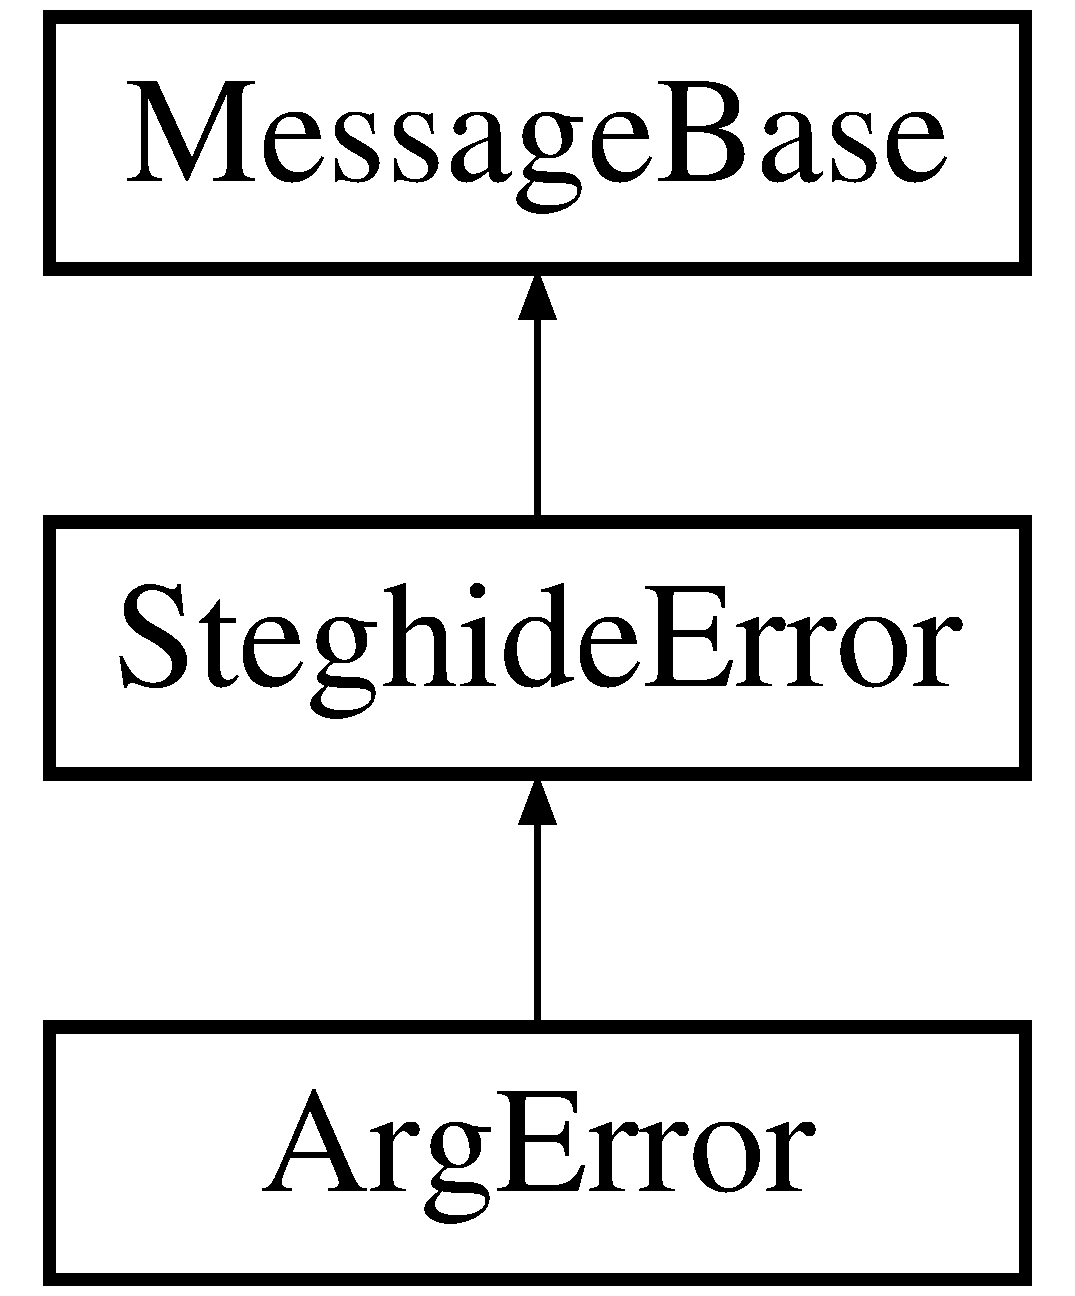
\includegraphics[height=3.000000cm]{classArgError}
\end{center}
\end{figure}
\subsection*{Public Member Functions}
\begin{DoxyCompactItemize}
\item 
\textbf{ Arg\+Error} (const char $\ast$msgfmt,...)
\item 
void \textbf{ print\+Message} (void) const
\end{DoxyCompactItemize}
\subsection*{Additional Inherited Members}


\subsection{Constructor \& Destructor Documentation}
\mbox{\label{classArgError_a5d7c1bc9f964d1b49ac4c70a0c9485b3}} 
\index{Arg\+Error@{Arg\+Error}!Arg\+Error@{Arg\+Error}}
\index{Arg\+Error@{Arg\+Error}!Arg\+Error@{Arg\+Error}}
\subsubsection{Arg\+Error()}
{\footnotesize\ttfamily Arg\+Error\+::\+Arg\+Error (\begin{DoxyParamCaption}\item[{const char $\ast$}]{msgfmt,  }\item[{}]{... }\end{DoxyParamCaption})}



\subsection{Member Function Documentation}
\mbox{\label{classArgError_a45233b131442b1af57c8278485856a83}} 
\index{Arg\+Error@{Arg\+Error}!print\+Message@{print\+Message}}
\index{print\+Message@{print\+Message}!Arg\+Error@{Arg\+Error}}
\subsubsection{print\+Message()}
{\footnotesize\ttfamily void Arg\+Error\+::print\+Message (\begin{DoxyParamCaption}\item[{void}]{ }\end{DoxyParamCaption}) const\hspace{0.3cm}{\ttfamily [virtual]}}



Reimplemented from \textbf{ Steghide\+Error} \doxyref{}{p.}{classSteghideError_a22d688da944706920f51159ebd0076d9}.



The documentation for this class was generated from the following files\+:\begin{DoxyCompactItemize}
\item 
\textbf{ error.\+h}\item 
\textbf{ error.\+cc}\end{DoxyCompactItemize}

\section{Arguments Class Reference}
\label{classArguments}\index{Arguments@{Arguments}}


parsing and data representation of command-\/line arguments  




{\ttfamily \#include $<$Arguments.\+h$>$}

\subsection*{Public Member Functions}
\begin{DoxyCompactItemize}
\item 
\textbf{ Arguments} (void)
\item 
\textbf{ Arguments} (int argc, char $\ast$argv[$\,$])
\item 
void \textbf{ parse} (void)
\item 
bool \textbf{ stdin\+\_\+isused} (void) const
\item 
std\+::string \textbf{ get\+Passphrase} (bool doublecheck=false)
\end{DoxyCompactItemize}
\subsection*{Public Attributes}
\begin{DoxyCompactItemize}
\item 
\textbf{ Arg\+Command} \textbf{ Command}
\begin{DoxyCompactList}\small\item\em the command to be executed in this session \end{DoxyCompactList}\item 
std\+::string \textbf{ Command\+String}
\begin{DoxyCompactList}\small\item\em the name of the command to be executed in this session (as supplied by the user) \end{DoxyCompactList}\item 
\textbf{ Arg\+String} \textbf{ Emb\+Fn}
\begin{DoxyCompactList}\small\item\em the embed file name, \char`\"{}\char`\"{} if stdin \end{DoxyCompactList}\item 
\textbf{ Arg\+String} \textbf{ Ext\+Fn}
\begin{DoxyCompactList}\small\item\em the extract file name, \char`\"{}\char`\"{} if stdout \end{DoxyCompactList}\item 
\textbf{ Arg\+String} \textbf{ Cvr\+Fn}
\begin{DoxyCompactList}\small\item\em the cover file name, \char`\"{}\char`\"{} if stdin \end{DoxyCompactList}\item 
\textbf{ Arg\+String} \textbf{ Stg\+Fn}
\begin{DoxyCompactList}\small\item\em the stego file name, \char`\"{}\char`\"{} if stdout/stdin \end{DoxyCompactList}\item 
\textbf{ Arg\+String} \textbf{ Passphrase}
\item 
\textbf{ Arg\+Bool} \textbf{ Checksum}
\item 
\textbf{ Arg\+Int} \textbf{ Compression}
\item 
\textbf{ Arg\+Bool} \textbf{ Embed\+Emb\+Fn}
\item 
\textbf{ Arg\+Enc\+Algo} \textbf{ Enc\+Algo}
\item 
\textbf{ Arg\+Enc\+Mode} \textbf{ Enc\+Mode}
\item 
\textbf{ Arg\+U\+Long} \textbf{ Radius}
\item 
\textbf{ Arg\+Float} \textbf{ Goal}
\item 
\textbf{ Arg\+Bool} \textbf{ Force}
\item 
\textbf{ Arg\+Verbosity} \textbf{ Verbosity}
\item 
\textbf{ Arg\+Debug\+Command} \textbf{ Debug\+Command}
\item 
\textbf{ Arg\+Bool} \textbf{ Check}
\item 
\textbf{ Arg\+String\+List} \textbf{ File\+List}
\item 
\textbf{ Arg\+U\+Int} \textbf{ Debug\+Level}
\item 
\textbf{ Arg\+U\+Int} \textbf{ Gml\+Graph\+Rec\+Depth}
\item 
\textbf{ Arg\+U\+Int} \textbf{ Gml\+Start\+Vertex}
\end{DoxyCompactItemize}
\subsection*{Private Types}
\begin{DoxyCompactItemize}
\item 
typedef std\+::vector$<$ std\+::string $>$\+::const\+\_\+iterator \textbf{ Arg\+It}
\end{DoxyCompactItemize}
\subsection*{Private Member Functions}
\begin{DoxyCompactItemize}
\item 
void \textbf{ parse\+\_\+\+Command} (\textbf{ Arg\+It} \&curarg)
\item 
bool \textbf{ parse\+\_\+\+Emb\+Fn} (\textbf{ Arg\+It} \&curarg)
\item 
bool \textbf{ parse\+\_\+\+Ext\+Fn} (\textbf{ Arg\+It} \&curarg)
\item 
bool \textbf{ parse\+\_\+\+Cvr\+Fn} (\textbf{ Arg\+It} \&curarg)
\item 
bool \textbf{ parse\+\_\+\+Stg\+Fn} (\textbf{ Arg\+It} \&curarg)
\item 
bool \textbf{ parse\+\_\+\+Passphrase} (\textbf{ Arg\+It} \&curarg)
\item 
bool \textbf{ parse\+\_\+\+Checksum} (\textbf{ Arg\+It} \&curarg)
\item 
bool \textbf{ parse\+\_\+\+Compression} (\textbf{ Arg\+It} \&curarg)
\item 
bool \textbf{ parse\+\_\+\+Embed\+Emb\+Fn} (\textbf{ Arg\+It} \&curarg)
\item 
bool \textbf{ parse\+\_\+\+Encryption} (\textbf{ Arg\+It} \&curarg)
\item 
bool \textbf{ parse\+\_\+\+Radius} (\textbf{ Arg\+It} \&curarg)
\item 
bool \textbf{ parse\+\_\+\+Goal} (\textbf{ Arg\+It} \&curarg)
\item 
bool \textbf{ parse\+\_\+\+Force} (\textbf{ Arg\+It} \&curarg)
\item 
bool \textbf{ parse\+\_\+\+Verbosity} (\textbf{ Arg\+It} \&curarg)
\item 
bool \textbf{ parse\+\_\+\+Debug} (\textbf{ Arg\+It} \&curarg)
\item 
void \textbf{ set\+Defaults} (void)
\end{DoxyCompactItemize}
\subsection*{Private Attributes}
\begin{DoxyCompactItemize}
\item 
std\+::vector$<$ std\+::string $>$ \textbf{ The\+Arguments}
\end{DoxyCompactItemize}
\subsection*{Static Private Attributes}
\begin{DoxyCompactItemize}
\item 
static const int \textbf{ No\+Compression} = 0
\item 
static const \textbf{ Encryption\+Algorithm} \textbf{ Default\+\_\+\+Enc\+Algo} = \textbf{ Encryption\+Algorithm} (\textbf{ Encryption\+Algorithm\+::\+N\+O\+NE})
\item 
static const \textbf{ Encryption\+Mode} \textbf{ Default\+\_\+\+Enc\+Mode} = \textbf{ Encryption\+Mode} (\textbf{ Encryption\+Mode\+::\+E\+CB})
\item 
static const bool \textbf{ Default\+\_\+\+Checksum} = true
\item 
static const int \textbf{ Default\+\_\+\+Compression} = 9
\item 
static const bool \textbf{ Default\+\_\+\+Embed\+Emb\+Fn} = true
\item 
static const bool \textbf{ Default\+\_\+\+Force} = false
\item 
static const \textbf{ V\+E\+R\+B\+O\+S\+I\+TY} \textbf{ Default\+\_\+\+Verbosity} = \textbf{ N\+O\+R\+M\+AL}
\item 
static const unsigned long \textbf{ Default\+\_\+\+Radius} = 0
\item 
static const unsigned int \textbf{ Max\+\_\+\+Algorithm} = 3
\item 
static const float \textbf{ Default\+\_\+\+Goal} = 100.\+0
\item 
static const \textbf{ D\+E\+B\+U\+G\+C\+O\+M\+M\+A\+ND} \textbf{ Default\+\_\+\+Debug\+Command} = \textbf{ N\+O\+NE}
\item 
static const bool \textbf{ Default\+\_\+\+Check} = false
\item 
static const unsigned int \textbf{ Default\+\_\+\+Debug\+Level} = 0
\item 
static const unsigned int \textbf{ Default\+\_\+\+Gml\+Graph\+Rec\+Depth} = 0
\item 
static const unsigned int \textbf{ Default\+\_\+\+Gml\+Start\+Vertex} = 0
\end{DoxyCompactItemize}


\subsection{Member Typedef Documentation}
\mbox{\label{classArguments_a364dd8c74c7f076209ae669e111b1e17}} 
\index{Arguments@{Arguments}!Arg\+It@{Arg\+It}}
\index{Arg\+It@{Arg\+It}!Arguments@{Arguments}}
\subsubsection{Arg\+It}
{\footnotesize\ttfamily typedef std\+::vector$<$std\+::string$>$\+::const\+\_\+iterator \textbf{ Arguments\+::\+Arg\+It}\hspace{0.3cm}{\ttfamily [private]}}



\subsection{Constructor \& Destructor Documentation}
\mbox{\label{classArguments_ad9fbdb9fcbe68000a87d15b4f60244fb}} 
\index{Arguments@{Arguments}!Arguments@{Arguments}}
\index{Arguments@{Arguments}!Arguments@{Arguments}}
\subsubsection{Arguments()\hspace{0.1cm}{\footnotesize\ttfamily [1/2]}}
{\footnotesize\ttfamily Arguments\+::\+Arguments (\begin{DoxyParamCaption}\item[{void}]{ }\end{DoxyParamCaption})\hspace{0.3cm}{\ttfamily [inline]}}

\mbox{\label{classArguments_a3d9dd7b675eac3c375c6b2e9bb13e896}} 
\index{Arguments@{Arguments}!Arguments@{Arguments}}
\index{Arguments@{Arguments}!Arguments@{Arguments}}
\subsubsection{Arguments()\hspace{0.1cm}{\footnotesize\ttfamily [2/2]}}
{\footnotesize\ttfamily Arguments\+::\+Arguments (\begin{DoxyParamCaption}\item[{int}]{argc,  }\item[{char $\ast$}]{argv[$\,$] }\end{DoxyParamCaption})}

initialize this \doxyref{Arguments}{p.}{classArguments} object with argc and argv 

\subsection{Member Function Documentation}
\mbox{\label{classArguments_a949a03365c6024f3e204b23d1c3bfbce}} 
\index{Arguments@{Arguments}!get\+Passphrase@{get\+Passphrase}}
\index{get\+Passphrase@{get\+Passphrase}!Arguments@{Arguments}}
\subsubsection{get\+Passphrase()}
{\footnotesize\ttfamily std\+::string Arguments\+::get\+Passphrase (\begin{DoxyParamCaption}\item[{bool}]{doublecheck = {\ttfamily false} }\end{DoxyParamCaption})}

\mbox{\label{classArguments_a73cb5b1d3960bba7552c02c3f4ca088c}} 
\index{Arguments@{Arguments}!parse@{parse}}
\index{parse@{parse}!Arguments@{Arguments}}
\subsubsection{parse()}
{\footnotesize\ttfamily void Arguments\+::parse (\begin{DoxyParamCaption}\item[{void}]{ }\end{DoxyParamCaption})}

parse Argc and Argv filling the Arg$\ast$ member variable for later access \mbox{\label{classArguments_af3321f349ed2a45f3cf469d73091ab19}} 
\index{Arguments@{Arguments}!parse\+\_\+\+Checksum@{parse\+\_\+\+Checksum}}
\index{parse\+\_\+\+Checksum@{parse\+\_\+\+Checksum}!Arguments@{Arguments}}
\subsubsection{parse\+\_\+\+Checksum()}
{\footnotesize\ttfamily bool Arguments\+::parse\+\_\+\+Checksum (\begin{DoxyParamCaption}\item[{\textbf{ Arg\+It} \&}]{curarg }\end{DoxyParamCaption})\hspace{0.3cm}{\ttfamily [private]}}

\mbox{\label{classArguments_a4c19459fe4d26d06abe71322198c3b99}} 
\index{Arguments@{Arguments}!parse\+\_\+\+Command@{parse\+\_\+\+Command}}
\index{parse\+\_\+\+Command@{parse\+\_\+\+Command}!Arguments@{Arguments}}
\subsubsection{parse\+\_\+\+Command()}
{\footnotesize\ttfamily void Arguments\+::parse\+\_\+\+Command (\begin{DoxyParamCaption}\item[{\textbf{ Arg\+It} \&}]{curarg }\end{DoxyParamCaption})\hspace{0.3cm}{\ttfamily [private]}}

parse the command

Note\+: parse\+\_\+\+Command is the only parse\+\_\+$\ast$ function that requires curarg to be a command. (because the command is the only argument with a fixed position). \mbox{\label{classArguments_ab457cbdbed4dfc7260c93c7dc51d866c}} 
\index{Arguments@{Arguments}!parse\+\_\+\+Compression@{parse\+\_\+\+Compression}}
\index{parse\+\_\+\+Compression@{parse\+\_\+\+Compression}!Arguments@{Arguments}}
\subsubsection{parse\+\_\+\+Compression()}
{\footnotesize\ttfamily bool Arguments\+::parse\+\_\+\+Compression (\begin{DoxyParamCaption}\item[{\textbf{ Arg\+It} \&}]{curarg }\end{DoxyParamCaption})\hspace{0.3cm}{\ttfamily [private]}}

\mbox{\label{classArguments_a2108bc892de8ddb4a2367e20c5b76be3}} 
\index{Arguments@{Arguments}!parse\+\_\+\+Cvr\+Fn@{parse\+\_\+\+Cvr\+Fn}}
\index{parse\+\_\+\+Cvr\+Fn@{parse\+\_\+\+Cvr\+Fn}!Arguments@{Arguments}}
\subsubsection{parse\+\_\+\+Cvr\+Fn()}
{\footnotesize\ttfamily bool Arguments\+::parse\+\_\+\+Cvr\+Fn (\begin{DoxyParamCaption}\item[{\textbf{ Arg\+It} \&}]{curarg }\end{DoxyParamCaption})\hspace{0.3cm}{\ttfamily [private]}}

\mbox{\label{classArguments_a17c957f70dc5f3c218601ac21db6b60c}} 
\index{Arguments@{Arguments}!parse\+\_\+\+Debug@{parse\+\_\+\+Debug}}
\index{parse\+\_\+\+Debug@{parse\+\_\+\+Debug}!Arguments@{Arguments}}
\subsubsection{parse\+\_\+\+Debug()}
{\footnotesize\ttfamily bool Arguments\+::parse\+\_\+\+Debug (\begin{DoxyParamCaption}\item[{\textbf{ Arg\+It} \&}]{curarg }\end{DoxyParamCaption})\hspace{0.3cm}{\ttfamily [private]}}

\mbox{\label{classArguments_a6acd02c15228d9579fe7ef91632560ff}} 
\index{Arguments@{Arguments}!parse\+\_\+\+Embed\+Emb\+Fn@{parse\+\_\+\+Embed\+Emb\+Fn}}
\index{parse\+\_\+\+Embed\+Emb\+Fn@{parse\+\_\+\+Embed\+Emb\+Fn}!Arguments@{Arguments}}
\subsubsection{parse\+\_\+\+Embed\+Emb\+Fn()}
{\footnotesize\ttfamily bool Arguments\+::parse\+\_\+\+Embed\+Emb\+Fn (\begin{DoxyParamCaption}\item[{\textbf{ Arg\+It} \&}]{curarg }\end{DoxyParamCaption})\hspace{0.3cm}{\ttfamily [private]}}

\mbox{\label{classArguments_a10c80492559837473315585d530df5ed}} 
\index{Arguments@{Arguments}!parse\+\_\+\+Emb\+Fn@{parse\+\_\+\+Emb\+Fn}}
\index{parse\+\_\+\+Emb\+Fn@{parse\+\_\+\+Emb\+Fn}!Arguments@{Arguments}}
\subsubsection{parse\+\_\+\+Emb\+Fn()}
{\footnotesize\ttfamily bool Arguments\+::parse\+\_\+\+Emb\+Fn (\begin{DoxyParamCaption}\item[{\textbf{ Arg\+It} \&}]{curarg }\end{DoxyParamCaption})\hspace{0.3cm}{\ttfamily [private]}}

test if curarg points to an emb filename argument and if yes\+: parse it \begin{DoxyReturn}{Returns}
true iff one or more arguments have been parsed 
\end{DoxyReturn}
\mbox{\label{classArguments_a3d389442fbcb40f80caaa050307956b1}} 
\index{Arguments@{Arguments}!parse\+\_\+\+Encryption@{parse\+\_\+\+Encryption}}
\index{parse\+\_\+\+Encryption@{parse\+\_\+\+Encryption}!Arguments@{Arguments}}
\subsubsection{parse\+\_\+\+Encryption()}
{\footnotesize\ttfamily bool Arguments\+::parse\+\_\+\+Encryption (\begin{DoxyParamCaption}\item[{\textbf{ Arg\+It} \&}]{curarg }\end{DoxyParamCaption})\hspace{0.3cm}{\ttfamily [private]}}

\mbox{\label{classArguments_abaca2ffefa0c28f34ddb7f67509c1678}} 
\index{Arguments@{Arguments}!parse\+\_\+\+Ext\+Fn@{parse\+\_\+\+Ext\+Fn}}
\index{parse\+\_\+\+Ext\+Fn@{parse\+\_\+\+Ext\+Fn}!Arguments@{Arguments}}
\subsubsection{parse\+\_\+\+Ext\+Fn()}
{\footnotesize\ttfamily bool Arguments\+::parse\+\_\+\+Ext\+Fn (\begin{DoxyParamCaption}\item[{\textbf{ Arg\+It} \&}]{curarg }\end{DoxyParamCaption})\hspace{0.3cm}{\ttfamily [private]}}

\mbox{\label{classArguments_abc68c17a514cc2b8153d04f4f8afb82f}} 
\index{Arguments@{Arguments}!parse\+\_\+\+Force@{parse\+\_\+\+Force}}
\index{parse\+\_\+\+Force@{parse\+\_\+\+Force}!Arguments@{Arguments}}
\subsubsection{parse\+\_\+\+Force()}
{\footnotesize\ttfamily bool Arguments\+::parse\+\_\+\+Force (\begin{DoxyParamCaption}\item[{\textbf{ Arg\+It} \&}]{curarg }\end{DoxyParamCaption})\hspace{0.3cm}{\ttfamily [private]}}

\mbox{\label{classArguments_a3610c5ee36796d30a24093a43c042f6b}} 
\index{Arguments@{Arguments}!parse\+\_\+\+Goal@{parse\+\_\+\+Goal}}
\index{parse\+\_\+\+Goal@{parse\+\_\+\+Goal}!Arguments@{Arguments}}
\subsubsection{parse\+\_\+\+Goal()}
{\footnotesize\ttfamily bool Arguments\+::parse\+\_\+\+Goal (\begin{DoxyParamCaption}\item[{\textbf{ Arg\+It} \&}]{curarg }\end{DoxyParamCaption})\hspace{0.3cm}{\ttfamily [private]}}

\mbox{\label{classArguments_a53cbd74d662bf1d6acd796965db1d332}} 
\index{Arguments@{Arguments}!parse\+\_\+\+Passphrase@{parse\+\_\+\+Passphrase}}
\index{parse\+\_\+\+Passphrase@{parse\+\_\+\+Passphrase}!Arguments@{Arguments}}
\subsubsection{parse\+\_\+\+Passphrase()}
{\footnotesize\ttfamily bool Arguments\+::parse\+\_\+\+Passphrase (\begin{DoxyParamCaption}\item[{\textbf{ Arg\+It} \&}]{curarg }\end{DoxyParamCaption})\hspace{0.3cm}{\ttfamily [private]}}

\mbox{\label{classArguments_ab3cae9862989c9da7539caccd64e347a}} 
\index{Arguments@{Arguments}!parse\+\_\+\+Radius@{parse\+\_\+\+Radius}}
\index{parse\+\_\+\+Radius@{parse\+\_\+\+Radius}!Arguments@{Arguments}}
\subsubsection{parse\+\_\+\+Radius()}
{\footnotesize\ttfamily bool Arguments\+::parse\+\_\+\+Radius (\begin{DoxyParamCaption}\item[{\textbf{ Arg\+It} \&}]{curarg }\end{DoxyParamCaption})\hspace{0.3cm}{\ttfamily [private]}}

\mbox{\label{classArguments_ace3cd4a045e1ea941861e6757c5e0658}} 
\index{Arguments@{Arguments}!parse\+\_\+\+Stg\+Fn@{parse\+\_\+\+Stg\+Fn}}
\index{parse\+\_\+\+Stg\+Fn@{parse\+\_\+\+Stg\+Fn}!Arguments@{Arguments}}
\subsubsection{parse\+\_\+\+Stg\+Fn()}
{\footnotesize\ttfamily bool Arguments\+::parse\+\_\+\+Stg\+Fn (\begin{DoxyParamCaption}\item[{\textbf{ Arg\+It} \&}]{curarg }\end{DoxyParamCaption})\hspace{0.3cm}{\ttfamily [private]}}

\mbox{\label{classArguments_a4eb8abe74f651b40166a0ff5c3db5e23}} 
\index{Arguments@{Arguments}!parse\+\_\+\+Verbosity@{parse\+\_\+\+Verbosity}}
\index{parse\+\_\+\+Verbosity@{parse\+\_\+\+Verbosity}!Arguments@{Arguments}}
\subsubsection{parse\+\_\+\+Verbosity()}
{\footnotesize\ttfamily bool Arguments\+::parse\+\_\+\+Verbosity (\begin{DoxyParamCaption}\item[{\textbf{ Arg\+It} \&}]{curarg }\end{DoxyParamCaption})\hspace{0.3cm}{\ttfamily [private]}}

\mbox{\label{classArguments_ae4dcc7d3f9551ae4a855fa1cae8897a5}} 
\index{Arguments@{Arguments}!set\+Defaults@{set\+Defaults}}
\index{set\+Defaults@{set\+Defaults}!Arguments@{Arguments}}
\subsubsection{set\+Defaults()}
{\footnotesize\ttfamily void Arguments\+::set\+Defaults (\begin{DoxyParamCaption}\item[{void}]{ }\end{DoxyParamCaption})\hspace{0.3cm}{\ttfamily [private]}}

\mbox{\label{classArguments_a5e63f21d6faa82884f7f2251790c46a5}} 
\index{Arguments@{Arguments}!stdin\+\_\+isused@{stdin\+\_\+isused}}
\index{stdin\+\_\+isused@{stdin\+\_\+isused}!Arguments@{Arguments}}
\subsubsection{stdin\+\_\+isused()}
{\footnotesize\ttfamily bool Arguments\+::stdin\+\_\+isused (\begin{DoxyParamCaption}\item[{void}]{ }\end{DoxyParamCaption}) const}

is standard input used ? -\/ according to the given arguments 

\subsection{Member Data Documentation}
\mbox{\label{classArguments_a603081ed6f56947f2fcd20829a715da9}} 
\index{Arguments@{Arguments}!Check@{Check}}
\index{Check@{Check}!Arguments@{Arguments}}
\subsubsection{Check}
{\footnotesize\ttfamily \textbf{ Arg\+Bool} Arguments\+::\+Check}

\mbox{\label{classArguments_a5005c1e69b276c098daec1bed4647739}} 
\index{Arguments@{Arguments}!Checksum@{Checksum}}
\index{Checksum@{Checksum}!Arguments@{Arguments}}
\subsubsection{Checksum}
{\footnotesize\ttfamily \textbf{ Arg\+Bool} Arguments\+::\+Checksum}

\mbox{\label{classArguments_acc9b16218e702644a8ecc276595552df}} 
\index{Arguments@{Arguments}!Command@{Command}}
\index{Command@{Command}!Arguments@{Arguments}}
\subsubsection{Command}
{\footnotesize\ttfamily \textbf{ Arg\+Command} Arguments\+::\+Command}

\mbox{\label{classArguments_a9f9727f4725bf93467a040b73bd54db5}} 
\index{Arguments@{Arguments}!Command\+String@{Command\+String}}
\index{Command\+String@{Command\+String}!Arguments@{Arguments}}
\subsubsection{Command\+String}
{\footnotesize\ttfamily std\+::string Arguments\+::\+Command\+String}

\mbox{\label{classArguments_a55855602c58dadc579b1553f80deae50}} 
\index{Arguments@{Arguments}!Compression@{Compression}}
\index{Compression@{Compression}!Arguments@{Arguments}}
\subsubsection{Compression}
{\footnotesize\ttfamily \textbf{ Arg\+Int} Arguments\+::\+Compression}

\mbox{\label{classArguments_ab6c97be04a624b0faa00b1eccd8e9ae8}} 
\index{Arguments@{Arguments}!Cvr\+Fn@{Cvr\+Fn}}
\index{Cvr\+Fn@{Cvr\+Fn}!Arguments@{Arguments}}
\subsubsection{Cvr\+Fn}
{\footnotesize\ttfamily \textbf{ Arg\+String} Arguments\+::\+Cvr\+Fn}

\mbox{\label{classArguments_aa41655956a8fe1ff0d0bafb8f763234a}} 
\index{Arguments@{Arguments}!Debug\+Command@{Debug\+Command}}
\index{Debug\+Command@{Debug\+Command}!Arguments@{Arguments}}
\subsubsection{Debug\+Command}
{\footnotesize\ttfamily \textbf{ Arg\+Debug\+Command} Arguments\+::\+Debug\+Command}

\mbox{\label{classArguments_aa5c0dfd8dd6858295f63e72d74e16db4}} 
\index{Arguments@{Arguments}!Debug\+Level@{Debug\+Level}}
\index{Debug\+Level@{Debug\+Level}!Arguments@{Arguments}}
\subsubsection{Debug\+Level}
{\footnotesize\ttfamily \textbf{ Arg\+U\+Int} Arguments\+::\+Debug\+Level}

\mbox{\label{classArguments_a321f4a5c1716d0b6419562000457bef8}} 
\index{Arguments@{Arguments}!Default\+\_\+\+Check@{Default\+\_\+\+Check}}
\index{Default\+\_\+\+Check@{Default\+\_\+\+Check}!Arguments@{Arguments}}
\subsubsection{Default\+\_\+\+Check}
{\footnotesize\ttfamily const bool Arguments\+::\+Default\+\_\+\+Check = false\hspace{0.3cm}{\ttfamily [static]}, {\ttfamily [private]}}

\mbox{\label{classArguments_aa465d1ac0962caa5479b51e36d8f6e41}} 
\index{Arguments@{Arguments}!Default\+\_\+\+Checksum@{Default\+\_\+\+Checksum}}
\index{Default\+\_\+\+Checksum@{Default\+\_\+\+Checksum}!Arguments@{Arguments}}
\subsubsection{Default\+\_\+\+Checksum}
{\footnotesize\ttfamily const bool Arguments\+::\+Default\+\_\+\+Checksum = true\hspace{0.3cm}{\ttfamily [static]}, {\ttfamily [private]}}

\mbox{\label{classArguments_ade01a1851efc374e35a5caef50a21dba}} 
\index{Arguments@{Arguments}!Default\+\_\+\+Compression@{Default\+\_\+\+Compression}}
\index{Default\+\_\+\+Compression@{Default\+\_\+\+Compression}!Arguments@{Arguments}}
\subsubsection{Default\+\_\+\+Compression}
{\footnotesize\ttfamily const int Arguments\+::\+Default\+\_\+\+Compression = 9\hspace{0.3cm}{\ttfamily [static]}, {\ttfamily [private]}}

\mbox{\label{classArguments_afa11c543146c6bb8d554088846767981}} 
\index{Arguments@{Arguments}!Default\+\_\+\+Debug\+Command@{Default\+\_\+\+Debug\+Command}}
\index{Default\+\_\+\+Debug\+Command@{Default\+\_\+\+Debug\+Command}!Arguments@{Arguments}}
\subsubsection{Default\+\_\+\+Debug\+Command}
{\footnotesize\ttfamily const \textbf{ D\+E\+B\+U\+G\+C\+O\+M\+M\+A\+ND} Arguments\+::\+Default\+\_\+\+Debug\+Command = \textbf{ N\+O\+NE}\hspace{0.3cm}{\ttfamily [static]}, {\ttfamily [private]}}

\mbox{\label{classArguments_a5accad7c3f9748b28f97dc09616f9248}} 
\index{Arguments@{Arguments}!Default\+\_\+\+Debug\+Level@{Default\+\_\+\+Debug\+Level}}
\index{Default\+\_\+\+Debug\+Level@{Default\+\_\+\+Debug\+Level}!Arguments@{Arguments}}
\subsubsection{Default\+\_\+\+Debug\+Level}
{\footnotesize\ttfamily const unsigned int Arguments\+::\+Default\+\_\+\+Debug\+Level = 0\hspace{0.3cm}{\ttfamily [static]}, {\ttfamily [private]}}

\mbox{\label{classArguments_a0e871d57240004c746b17db3dd73e2fe}} 
\index{Arguments@{Arguments}!Default\+\_\+\+Embed\+Emb\+Fn@{Default\+\_\+\+Embed\+Emb\+Fn}}
\index{Default\+\_\+\+Embed\+Emb\+Fn@{Default\+\_\+\+Embed\+Emb\+Fn}!Arguments@{Arguments}}
\subsubsection{Default\+\_\+\+Embed\+Emb\+Fn}
{\footnotesize\ttfamily const bool Arguments\+::\+Default\+\_\+\+Embed\+Emb\+Fn = true\hspace{0.3cm}{\ttfamily [static]}, {\ttfamily [private]}}

\mbox{\label{classArguments_a7087a2e48728335a1cdd736e55cccccf}} 
\index{Arguments@{Arguments}!Default\+\_\+\+Enc\+Algo@{Default\+\_\+\+Enc\+Algo}}
\index{Default\+\_\+\+Enc\+Algo@{Default\+\_\+\+Enc\+Algo}!Arguments@{Arguments}}
\subsubsection{Default\+\_\+\+Enc\+Algo}
{\footnotesize\ttfamily const \textbf{ Encryption\+Algorithm} Arguments\+::\+Default\+\_\+\+Enc\+Algo = \textbf{ Encryption\+Algorithm} (\textbf{ Encryption\+Algorithm\+::\+N\+O\+NE})\hspace{0.3cm}{\ttfamily [static]}, {\ttfamily [private]}}

\mbox{\label{classArguments_ade7c80528dc147a4258ebdd3deab6d11}} 
\index{Arguments@{Arguments}!Default\+\_\+\+Enc\+Mode@{Default\+\_\+\+Enc\+Mode}}
\index{Default\+\_\+\+Enc\+Mode@{Default\+\_\+\+Enc\+Mode}!Arguments@{Arguments}}
\subsubsection{Default\+\_\+\+Enc\+Mode}
{\footnotesize\ttfamily const \textbf{ Encryption\+Mode} Arguments\+::\+Default\+\_\+\+Enc\+Mode = \textbf{ Encryption\+Mode} (\textbf{ Encryption\+Mode\+::\+E\+CB})\hspace{0.3cm}{\ttfamily [static]}, {\ttfamily [private]}}

\mbox{\label{classArguments_acdaa1bdc3e4cf5c4022e7240c7175f9b}} 
\index{Arguments@{Arguments}!Default\+\_\+\+Force@{Default\+\_\+\+Force}}
\index{Default\+\_\+\+Force@{Default\+\_\+\+Force}!Arguments@{Arguments}}
\subsubsection{Default\+\_\+\+Force}
{\footnotesize\ttfamily const bool Arguments\+::\+Default\+\_\+\+Force = false\hspace{0.3cm}{\ttfamily [static]}, {\ttfamily [private]}}

\mbox{\label{classArguments_a038246ddc2a99efe9edd76488e074662}} 
\index{Arguments@{Arguments}!Default\+\_\+\+Gml\+Graph\+Rec\+Depth@{Default\+\_\+\+Gml\+Graph\+Rec\+Depth}}
\index{Default\+\_\+\+Gml\+Graph\+Rec\+Depth@{Default\+\_\+\+Gml\+Graph\+Rec\+Depth}!Arguments@{Arguments}}
\subsubsection{Default\+\_\+\+Gml\+Graph\+Rec\+Depth}
{\footnotesize\ttfamily const unsigned int Arguments\+::\+Default\+\_\+\+Gml\+Graph\+Rec\+Depth = 0\hspace{0.3cm}{\ttfamily [static]}, {\ttfamily [private]}}

\mbox{\label{classArguments_a9d5b4d02ff13f9c5cd189a39f7c7cfc2}} 
\index{Arguments@{Arguments}!Default\+\_\+\+Gml\+Start\+Vertex@{Default\+\_\+\+Gml\+Start\+Vertex}}
\index{Default\+\_\+\+Gml\+Start\+Vertex@{Default\+\_\+\+Gml\+Start\+Vertex}!Arguments@{Arguments}}
\subsubsection{Default\+\_\+\+Gml\+Start\+Vertex}
{\footnotesize\ttfamily const unsigned int Arguments\+::\+Default\+\_\+\+Gml\+Start\+Vertex = 0\hspace{0.3cm}{\ttfamily [static]}, {\ttfamily [private]}}

\mbox{\label{classArguments_a1849af56dcb024147fc5b4cc9d12b7c4}} 
\index{Arguments@{Arguments}!Default\+\_\+\+Goal@{Default\+\_\+\+Goal}}
\index{Default\+\_\+\+Goal@{Default\+\_\+\+Goal}!Arguments@{Arguments}}
\subsubsection{Default\+\_\+\+Goal}
{\footnotesize\ttfamily const float Arguments\+::\+Default\+\_\+\+Goal = 100.\+0\hspace{0.3cm}{\ttfamily [static]}, {\ttfamily [private]}}

\mbox{\label{classArguments_afdc4e2ebb15490487bf1bf6c413249b5}} 
\index{Arguments@{Arguments}!Default\+\_\+\+Radius@{Default\+\_\+\+Radius}}
\index{Default\+\_\+\+Radius@{Default\+\_\+\+Radius}!Arguments@{Arguments}}
\subsubsection{Default\+\_\+\+Radius}
{\footnotesize\ttfamily const unsigned long Arguments\+::\+Default\+\_\+\+Radius = 0\hspace{0.3cm}{\ttfamily [static]}, {\ttfamily [private]}}

\mbox{\label{classArguments_a22e001d707e30969e6e6fa8e08f3dc14}} 
\index{Arguments@{Arguments}!Default\+\_\+\+Verbosity@{Default\+\_\+\+Verbosity}}
\index{Default\+\_\+\+Verbosity@{Default\+\_\+\+Verbosity}!Arguments@{Arguments}}
\subsubsection{Default\+\_\+\+Verbosity}
{\footnotesize\ttfamily const \textbf{ V\+E\+R\+B\+O\+S\+I\+TY} Arguments\+::\+Default\+\_\+\+Verbosity = \textbf{ N\+O\+R\+M\+AL}\hspace{0.3cm}{\ttfamily [static]}, {\ttfamily [private]}}

\mbox{\label{classArguments_a8474452b8592fab92462e00dc961c81e}} 
\index{Arguments@{Arguments}!Embed\+Emb\+Fn@{Embed\+Emb\+Fn}}
\index{Embed\+Emb\+Fn@{Embed\+Emb\+Fn}!Arguments@{Arguments}}
\subsubsection{Embed\+Emb\+Fn}
{\footnotesize\ttfamily \textbf{ Arg\+Bool} Arguments\+::\+Embed\+Emb\+Fn}

\mbox{\label{classArguments_a12c3a28f09e610c0f952037681b049cb}} 
\index{Arguments@{Arguments}!Emb\+Fn@{Emb\+Fn}}
\index{Emb\+Fn@{Emb\+Fn}!Arguments@{Arguments}}
\subsubsection{Emb\+Fn}
{\footnotesize\ttfamily \textbf{ Arg\+String} Arguments\+::\+Emb\+Fn}

\mbox{\label{classArguments_acd26418c75e4a897656880f6f1188fe9}} 
\index{Arguments@{Arguments}!Enc\+Algo@{Enc\+Algo}}
\index{Enc\+Algo@{Enc\+Algo}!Arguments@{Arguments}}
\subsubsection{Enc\+Algo}
{\footnotesize\ttfamily \textbf{ Arg\+Enc\+Algo} Arguments\+::\+Enc\+Algo}

\mbox{\label{classArguments_a76fd62516a7da91baf92e75b5e3e74fb}} 
\index{Arguments@{Arguments}!Enc\+Mode@{Enc\+Mode}}
\index{Enc\+Mode@{Enc\+Mode}!Arguments@{Arguments}}
\subsubsection{Enc\+Mode}
{\footnotesize\ttfamily \textbf{ Arg\+Enc\+Mode} Arguments\+::\+Enc\+Mode}

\mbox{\label{classArguments_a937a64373e35f61d3ddabfad7e9e6930}} 
\index{Arguments@{Arguments}!Ext\+Fn@{Ext\+Fn}}
\index{Ext\+Fn@{Ext\+Fn}!Arguments@{Arguments}}
\subsubsection{Ext\+Fn}
{\footnotesize\ttfamily \textbf{ Arg\+String} Arguments\+::\+Ext\+Fn}

\mbox{\label{classArguments_a49c2c2ba850aabeb651efa64df4d58a1}} 
\index{Arguments@{Arguments}!File\+List@{File\+List}}
\index{File\+List@{File\+List}!Arguments@{Arguments}}
\subsubsection{File\+List}
{\footnotesize\ttfamily \textbf{ Arg\+String\+List} Arguments\+::\+File\+List}

\mbox{\label{classArguments_ac9cc71e9d2dd92a3d332a71566596788}} 
\index{Arguments@{Arguments}!Force@{Force}}
\index{Force@{Force}!Arguments@{Arguments}}
\subsubsection{Force}
{\footnotesize\ttfamily \textbf{ Arg\+Bool} Arguments\+::\+Force}

\mbox{\label{classArguments_a52bec7af0fe1355b2dd336839fe35579}} 
\index{Arguments@{Arguments}!Gml\+Graph\+Rec\+Depth@{Gml\+Graph\+Rec\+Depth}}
\index{Gml\+Graph\+Rec\+Depth@{Gml\+Graph\+Rec\+Depth}!Arguments@{Arguments}}
\subsubsection{Gml\+Graph\+Rec\+Depth}
{\footnotesize\ttfamily \textbf{ Arg\+U\+Int} Arguments\+::\+Gml\+Graph\+Rec\+Depth}

\mbox{\label{classArguments_abd98a39911a586ec9bd28834251aac09}} 
\index{Arguments@{Arguments}!Gml\+Start\+Vertex@{Gml\+Start\+Vertex}}
\index{Gml\+Start\+Vertex@{Gml\+Start\+Vertex}!Arguments@{Arguments}}
\subsubsection{Gml\+Start\+Vertex}
{\footnotesize\ttfamily \textbf{ Arg\+U\+Int} Arguments\+::\+Gml\+Start\+Vertex}

\mbox{\label{classArguments_a813e8d4cdc854ea5d9496757a3b0dd55}} 
\index{Arguments@{Arguments}!Goal@{Goal}}
\index{Goal@{Goal}!Arguments@{Arguments}}
\subsubsection{Goal}
{\footnotesize\ttfamily \textbf{ Arg\+Float} Arguments\+::\+Goal}

\mbox{\label{classArguments_aeb4d6ca9411772d61096e0b52996be04}} 
\index{Arguments@{Arguments}!Max\+\_\+\+Algorithm@{Max\+\_\+\+Algorithm}}
\index{Max\+\_\+\+Algorithm@{Max\+\_\+\+Algorithm}!Arguments@{Arguments}}
\subsubsection{Max\+\_\+\+Algorithm}
{\footnotesize\ttfamily const unsigned int Arguments\+::\+Max\+\_\+\+Algorithm = 3\hspace{0.3cm}{\ttfamily [static]}, {\ttfamily [private]}}

\mbox{\label{classArguments_a7433848d69f277be30c9a2bc57af707d}} 
\index{Arguments@{Arguments}!No\+Compression@{No\+Compression}}
\index{No\+Compression@{No\+Compression}!Arguments@{Arguments}}
\subsubsection{No\+Compression}
{\footnotesize\ttfamily const int Arguments\+::\+No\+Compression = 0\hspace{0.3cm}{\ttfamily [static]}, {\ttfamily [private]}}

\mbox{\label{classArguments_a3f5592cbcf337f3c8a3dc7a81658b872}} 
\index{Arguments@{Arguments}!Passphrase@{Passphrase}}
\index{Passphrase@{Passphrase}!Arguments@{Arguments}}
\subsubsection{Passphrase}
{\footnotesize\ttfamily \textbf{ Arg\+String} Arguments\+::\+Passphrase}

\mbox{\label{classArguments_a25b945c660b5e092126442457341f4d6}} 
\index{Arguments@{Arguments}!Radius@{Radius}}
\index{Radius@{Radius}!Arguments@{Arguments}}
\subsubsection{Radius}
{\footnotesize\ttfamily \textbf{ Arg\+U\+Long} Arguments\+::\+Radius}

\mbox{\label{classArguments_a76c6fd6c5e80777b4602027bef5c6c1d}} 
\index{Arguments@{Arguments}!Stg\+Fn@{Stg\+Fn}}
\index{Stg\+Fn@{Stg\+Fn}!Arguments@{Arguments}}
\subsubsection{Stg\+Fn}
{\footnotesize\ttfamily \textbf{ Arg\+String} Arguments\+::\+Stg\+Fn}

\mbox{\label{classArguments_a51c12d145b4a05427462ce475dd9a4d7}} 
\index{Arguments@{Arguments}!The\+Arguments@{The\+Arguments}}
\index{The\+Arguments@{The\+Arguments}!Arguments@{Arguments}}
\subsubsection{The\+Arguments}
{\footnotesize\ttfamily std\+::vector$<$std\+::string$>$ Arguments\+::\+The\+Arguments\hspace{0.3cm}{\ttfamily [private]}}

\mbox{\label{classArguments_a332013d89bb1d0133fa115c46155526a}} 
\index{Arguments@{Arguments}!Verbosity@{Verbosity}}
\index{Verbosity@{Verbosity}!Arguments@{Arguments}}
\subsubsection{Verbosity}
{\footnotesize\ttfamily \textbf{ Arg\+Verbosity} Arguments\+::\+Verbosity}



The documentation for this class was generated from the following files\+:\begin{DoxyCompactItemize}
\item 
\textbf{ Arguments.\+h}\item 
\textbf{ Arguments.\+cc}\end{DoxyCompactItemize}

\section{Assertion\+Failed Class Reference}
\label{classAssertionFailed}\index{Assertion\+Failed@{Assertion\+Failed}}


{\ttfamily \#include $<$Assertion\+Failed.\+h$>$}

Inheritance diagram for Assertion\+Failed\+:\begin{figure}[H]
\begin{center}
\leavevmode
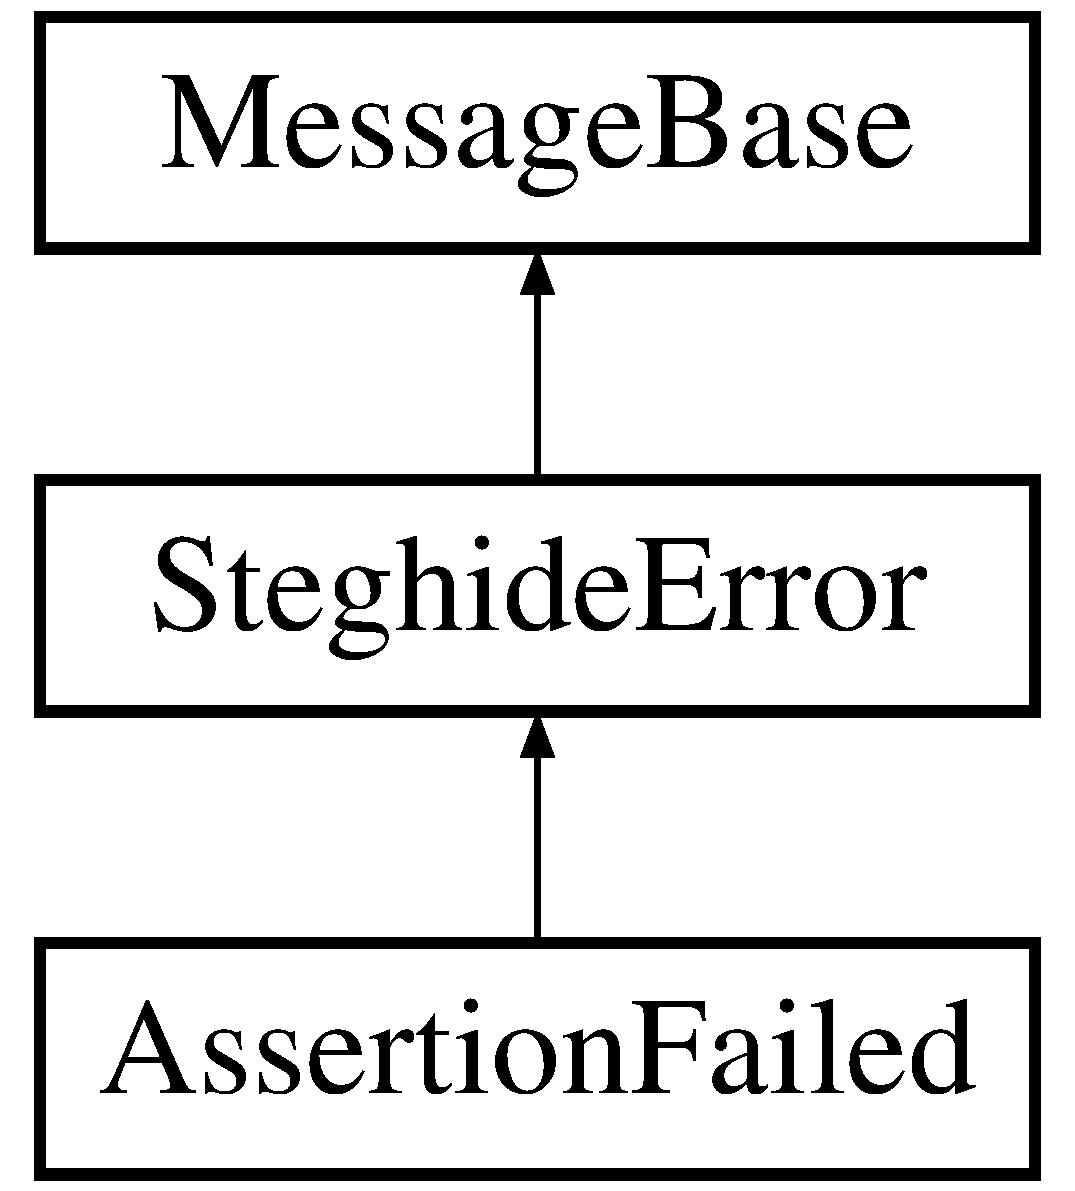
\includegraphics[height=3.000000cm]{classAssertionFailed}
\end{center}
\end{figure}
\subsection*{Public Member Functions}
\begin{DoxyCompactItemize}
\item 
\textbf{ Assertion\+Failed} (const char $\ast$fn, unsigned int l)
\item 
void \textbf{ print\+Message} (void) const
\end{DoxyCompactItemize}
\subsection*{Private Member Functions}
\begin{DoxyCompactItemize}
\item 
char $\ast$ \textbf{ strip\+Dir} (const char $\ast$fn)
\end{DoxyCompactItemize}
\subsection*{Additional Inherited Members}


\subsection{Constructor \& Destructor Documentation}
\mbox{\label{classAssertionFailed_adc29e1da3e62c0bb30ca7e34a0f65bf6}} 
\index{Assertion\+Failed@{Assertion\+Failed}!Assertion\+Failed@{Assertion\+Failed}}
\index{Assertion\+Failed@{Assertion\+Failed}!Assertion\+Failed@{Assertion\+Failed}}
\subsubsection{Assertion\+Failed()}
{\footnotesize\ttfamily Assertion\+Failed\+::\+Assertion\+Failed (\begin{DoxyParamCaption}\item[{const char $\ast$}]{fn,  }\item[{unsigned int}]{l }\end{DoxyParamCaption})\hspace{0.3cm}{\ttfamily [inline]}}



\subsection{Member Function Documentation}
\mbox{\label{classAssertionFailed_acab14a3cc730015f7c8c76a17d0b347c}} 
\index{Assertion\+Failed@{Assertion\+Failed}!print\+Message@{print\+Message}}
\index{print\+Message@{print\+Message}!Assertion\+Failed@{Assertion\+Failed}}
\subsubsection{print\+Message()}
{\footnotesize\ttfamily void Assertion\+Failed\+::print\+Message (\begin{DoxyParamCaption}\item[{void}]{ }\end{DoxyParamCaption}) const\hspace{0.3cm}{\ttfamily [virtual]}}



Reimplemented from \textbf{ Steghide\+Error} \doxyref{}{p.}{classSteghideError_a22d688da944706920f51159ebd0076d9}.

\mbox{\label{classAssertionFailed_a40dcfe5b67eaea9dd37ac4f72efabccd}} 
\index{Assertion\+Failed@{Assertion\+Failed}!strip\+Dir@{strip\+Dir}}
\index{strip\+Dir@{strip\+Dir}!Assertion\+Failed@{Assertion\+Failed}}
\subsubsection{strip\+Dir()}
{\footnotesize\ttfamily char $\ast$ Assertion\+Failed\+::strip\+Dir (\begin{DoxyParamCaption}\item[{const char $\ast$}]{fn }\end{DoxyParamCaption})\hspace{0.3cm}{\ttfamily [private]}}



The documentation for this class was generated from the following files\+:\begin{DoxyCompactItemize}
\item 
\textbf{ Assertion\+Failed.\+h}\item 
\textbf{ Assertion\+Failed.\+cc}\end{DoxyCompactItemize}

\section{Audio\+Data Class Reference}
\label{classAudioData}\index{Audio\+Data@{Audio\+Data}}


interface definition for \doxyref{Audio\+Data}{p.}{classAudioData} objects.  




{\ttfamily \#include $<$Audio\+Data.\+h$>$}

Inheritance diagram for Audio\+Data\+:\begin{figure}[H]
\begin{center}
\leavevmode
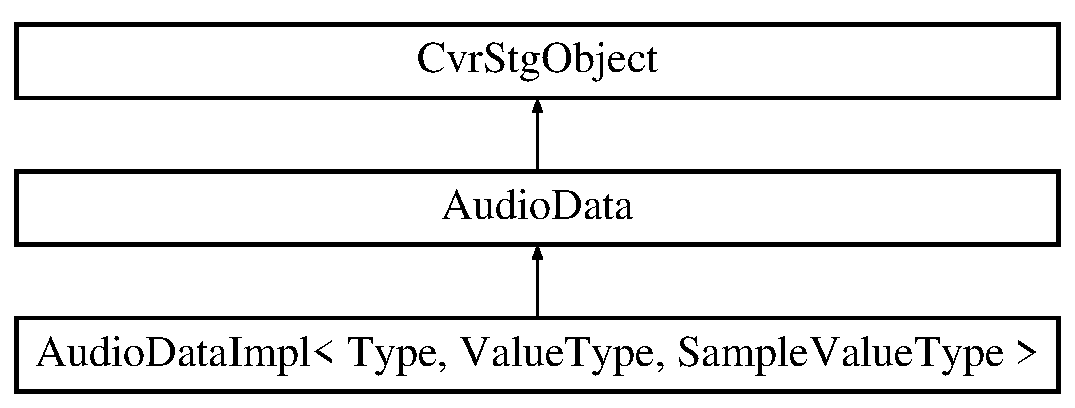
\includegraphics[height=3.000000cm]{classAudioData}
\end{center}
\end{figure}
\subsection*{Public Member Functions}
\begin{DoxyCompactItemize}
\item 
virtual void \textbf{ read} (\textbf{ Binary\+IO} $\ast$io, \textbf{ U\+W\+O\+R\+D32} n=\textbf{ No\+Limit})=0
\item 
virtual void \textbf{ write} (\textbf{ Binary\+IO} $\ast$io, \textbf{ U\+W\+O\+R\+D32} n=\textbf{ No\+Limit})=0
\end{DoxyCompactItemize}
\subsection*{Static Public Attributes}
\begin{DoxyCompactItemize}
\item 
static const \textbf{ U\+W\+O\+R\+D32} \textbf{ No\+Limit} = 0
\begin{DoxyCompactList}\small\item\em constant that can be used as parameter to read and write to indicate that there is no limit \end{DoxyCompactList}\end{DoxyCompactItemize}


\subsection{Detailed Description}
This class is necessary to provide one common base class for all types of audio data, i.\+e. all different instances of \doxyref{Audio\+Data\+Impl}{p.}{classAudioDataImpl}. 

\subsection{Member Function Documentation}
\mbox{\label{classAudioData_aa3ac98fcebcd5e2f5376464b08212e58}} 
\index{Audio\+Data@{Audio\+Data}!read@{read}}
\index{read@{read}!Audio\+Data@{Audio\+Data}}
\subsubsection{read()}
{\footnotesize\ttfamily virtual void Audio\+Data\+::read (\begin{DoxyParamCaption}\item[{\textbf{ Binary\+IO} $\ast$}]{io,  }\item[{\textbf{ U\+W\+O\+R\+D32}}]{n = {\ttfamily \textbf{ No\+Limit}} }\end{DoxyParamCaption})\hspace{0.3cm}{\ttfamily [pure virtual]}}



Implemented in \textbf{ Audio\+Data\+Impl$<$ Type, Value\+Type, Sample\+Value\+Type $>$} \doxyref{}{p.}{classAudioDataImpl_a6c8105d5fceee538b423e8b137ecd3ab}.

\mbox{\label{classAudioData_aedc90f99fe9da3fd0012e2fb79403d88}} 
\index{Audio\+Data@{Audio\+Data}!write@{write}}
\index{write@{write}!Audio\+Data@{Audio\+Data}}
\subsubsection{write()}
{\footnotesize\ttfamily virtual void Audio\+Data\+::write (\begin{DoxyParamCaption}\item[{\textbf{ Binary\+IO} $\ast$}]{io,  }\item[{\textbf{ U\+W\+O\+R\+D32}}]{n = {\ttfamily \textbf{ No\+Limit}} }\end{DoxyParamCaption})\hspace{0.3cm}{\ttfamily [pure virtual]}}



Implemented in \textbf{ Audio\+Data\+Impl$<$ Type, Value\+Type, Sample\+Value\+Type $>$} \doxyref{}{p.}{classAudioDataImpl_a66671d9d8ee1c2322f4226dad81e257c}.



\subsection{Member Data Documentation}
\mbox{\label{classAudioData_ae4e3f99d2d21a5982aa1f76d78367cf6}} 
\index{Audio\+Data@{Audio\+Data}!No\+Limit@{No\+Limit}}
\index{No\+Limit@{No\+Limit}!Audio\+Data@{Audio\+Data}}
\subsubsection{No\+Limit}
{\footnotesize\ttfamily const \textbf{ U\+W\+O\+R\+D32} Audio\+Data\+::\+No\+Limit = 0\hspace{0.3cm}{\ttfamily [static]}}



The documentation for this class was generated from the following file\+:\begin{DoxyCompactItemize}
\item 
\textbf{ Audio\+Data.\+h}\end{DoxyCompactItemize}

\section{Audio\+Data\+Impl$<$ Type, Value\+Type, Sample\+Value\+Type $>$ Class Template Reference}
\label{classAudioDataImpl}\index{Audio\+Data\+Impl$<$ Type, Value\+Type, Sample\+Value\+Type $>$@{Audio\+Data\+Impl$<$ Type, Value\+Type, Sample\+Value\+Type $>$}}


implementation of the Audio\+Data-\/\+Interface  




{\ttfamily \#include $<$Audio\+Data.\+h$>$}

Inheritance diagram for Audio\+Data\+Impl$<$ Type, Value\+Type, Sample\+Value\+Type $>$\+:\begin{figure}[H]
\begin{center}
\leavevmode
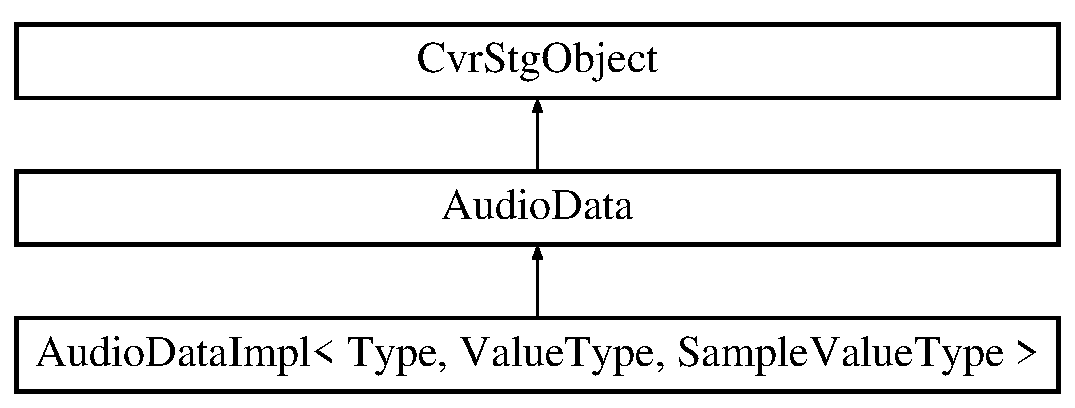
\includegraphics[height=3.000000cm]{classAudioDataImpl}
\end{center}
\end{figure}
\subsection*{Public Member Functions}
\begin{DoxyCompactItemize}
\item 
\textbf{ Audio\+Data\+Impl} (\textbf{ Cvr\+Stg\+File} $\ast$f)
\item 
virtual \textbf{ $\sim$\+Audio\+Data\+Impl} (void)
\item 
void \textbf{ read} (\textbf{ Binary\+IO} $\ast$io, \textbf{ U\+W\+O\+R\+D32} n=\textbf{ Audio\+Data\+::\+No\+Limit})
\item 
void \textbf{ write} (\textbf{ Binary\+IO} $\ast$io, \textbf{ U\+W\+O\+R\+D32} n=\textbf{ Audio\+Data\+::\+No\+Limit})
\item 
unsigned long \textbf{ get\+Num\+Samples} (void) const
\item 
\textbf{ Sample\+Value} $\ast$ \textbf{ get\+Sample\+Value} (const \textbf{ Sample\+Pos} pos) const
\item 
void \textbf{ replace\+Sample} (const \textbf{ Sample\+Pos} pos, const \textbf{ Sample\+Value} $\ast$s)
\end{DoxyCompactItemize}
\subsection*{Private Member Functions}
\begin{DoxyCompactItemize}
\item 
Value\+Type \textbf{ read\+Value} (\textbf{ Binary\+IO} $\ast$io) const
\item 
void \textbf{ write\+Value} (\textbf{ Binary\+IO} $\ast$io, Value\+Type v) const
\end{DoxyCompactItemize}
\subsection*{Private Attributes}
\begin{DoxyCompactItemize}
\item 
std\+::vector$<$ Value\+Type $>$ \textbf{ Data}
\item 
\textbf{ Cvr\+Stg\+File} $\ast$ \textbf{ The\+Cvr\+Stg\+File}
\end{DoxyCompactItemize}
\subsection*{Additional Inherited Members}


\subsection{Constructor \& Destructor Documentation}
\mbox{\label{classAudioDataImpl_a5775d49843e1ab609610f6cf4efb178e}} 
\index{Audio\+Data\+Impl@{Audio\+Data\+Impl}!Audio\+Data\+Impl@{Audio\+Data\+Impl}}
\index{Audio\+Data\+Impl@{Audio\+Data\+Impl}!Audio\+Data\+Impl@{Audio\+Data\+Impl}}
\subsubsection{Audio\+Data\+Impl()}
{\footnotesize\ttfamily template$<$A\+U\+D\+I\+O\+S\+A\+M\+P\+L\+E\+T\+Y\+PE Type, class Value\+Type , class Sample\+Value\+Type  = Audio\+Sample\+Value$<$\+Type,\+Value\+Type$>$$>$ \\
\textbf{ Audio\+Data\+Impl}$<$ Type, Value\+Type, Sample\+Value\+Type $>$\+::\textbf{ Audio\+Data\+Impl} (\begin{DoxyParamCaption}\item[{\textbf{ Cvr\+Stg\+File} $\ast$}]{f }\end{DoxyParamCaption})\hspace{0.3cm}{\ttfamily [inline]}}

\mbox{\label{classAudioDataImpl_a700d701bf616673b6f09d761ea31307d}} 
\index{Audio\+Data\+Impl@{Audio\+Data\+Impl}!````~Audio\+Data\+Impl@{$\sim$\+Audio\+Data\+Impl}}
\index{````~Audio\+Data\+Impl@{$\sim$\+Audio\+Data\+Impl}!Audio\+Data\+Impl@{Audio\+Data\+Impl}}
\subsubsection{$\sim$\+Audio\+Data\+Impl()}
{\footnotesize\ttfamily template$<$A\+U\+D\+I\+O\+S\+A\+M\+P\+L\+E\+T\+Y\+PE Type, class Value\+Type , class Sample\+Value\+Type  = Audio\+Sample\+Value$<$\+Type,\+Value\+Type$>$$>$ \\
virtual \textbf{ Audio\+Data\+Impl}$<$ Type, Value\+Type, Sample\+Value\+Type $>$\+::$\sim$\textbf{ Audio\+Data\+Impl} (\begin{DoxyParamCaption}\item[{void}]{ }\end{DoxyParamCaption})\hspace{0.3cm}{\ttfamily [inline]}, {\ttfamily [virtual]}}



\subsection{Member Function Documentation}
\mbox{\label{classAudioDataImpl_a84f684e5b78a19e9b9ecfc530589706a}} 
\index{Audio\+Data\+Impl@{Audio\+Data\+Impl}!get\+Num\+Samples@{get\+Num\+Samples}}
\index{get\+Num\+Samples@{get\+Num\+Samples}!Audio\+Data\+Impl@{Audio\+Data\+Impl}}
\subsubsection{get\+Num\+Samples()}
{\footnotesize\ttfamily template$<$A\+U\+D\+I\+O\+S\+A\+M\+P\+L\+E\+T\+Y\+PE Type, class Value\+Type , class Sample\+Value\+Type $>$ \\
unsigned long \textbf{ Audio\+Data\+Impl}$<$ Type, Value\+Type, Sample\+Value\+Type $>$\+::get\+Num\+Samples (\begin{DoxyParamCaption}\item[{void}]{ }\end{DoxyParamCaption}) const\hspace{0.3cm}{\ttfamily [virtual]}}

get the number of samples in this \doxyref{Cvr\+Stg\+Object}{p.}{classCvrStgObject} 

Implements \textbf{ Cvr\+Stg\+Object} \doxyref{}{p.}{classCvrStgObject_a80ae8f095b66683e5207adf8ff8265b4}.

\mbox{\label{classAudioDataImpl_a52990850bb0a8a108108f70f378d9461}} 
\index{Audio\+Data\+Impl@{Audio\+Data\+Impl}!get\+Sample\+Value@{get\+Sample\+Value}}
\index{get\+Sample\+Value@{get\+Sample\+Value}!Audio\+Data\+Impl@{Audio\+Data\+Impl}}
\subsubsection{get\+Sample\+Value()}
{\footnotesize\ttfamily template$<$A\+U\+D\+I\+O\+S\+A\+M\+P\+L\+E\+T\+Y\+PE Type, class Value\+Type , class Sample\+Value\+Type $>$ \\
\textbf{ Sample\+Value} $\ast$ \textbf{ Audio\+Data\+Impl}$<$ Type, Value\+Type, Sample\+Value\+Type $>$\+::get\+Sample\+Value (\begin{DoxyParamCaption}\item[{const \textbf{ Sample\+Pos}}]{pos }\end{DoxyParamCaption}) const\hspace{0.3cm}{\ttfamily [virtual]}}

get the sample at position pos 
\begin{DoxyParams}{Parameters}
{\em pos} & the position of a sample (must be in 0...\doxyref{get\+Num\+Samples()}{p.}{classAudioDataImpl_a84f684e5b78a19e9b9ecfc530589706a}-\/1) \\
\hline
\end{DoxyParams}
\begin{DoxyReturn}{Returns}
the sample at the given position
\end{DoxyReturn}
The sample object is created in this function and should be deleted by the caller. The derived class should check the condition(s) given above in its Implementation of this function. 

Implements \textbf{ Cvr\+Stg\+Object} \doxyref{}{p.}{classCvrStgObject_ac77a8da85a4f7b53e2166e990dfaa4f2}.

\mbox{\label{classAudioDataImpl_a6c8105d5fceee538b423e8b137ecd3ab}} 
\index{Audio\+Data\+Impl@{Audio\+Data\+Impl}!read@{read}}
\index{read@{read}!Audio\+Data\+Impl@{Audio\+Data\+Impl}}
\subsubsection{read()}
{\footnotesize\ttfamily template$<$A\+U\+D\+I\+O\+S\+A\+M\+P\+L\+E\+T\+Y\+PE Type, class Value\+Type , class Sample\+Value\+Type $>$ \\
void \textbf{ Audio\+Data\+Impl}$<$ Type, Value\+Type, Sample\+Value\+Type $>$\+::read (\begin{DoxyParamCaption}\item[{\textbf{ Binary\+IO} $\ast$}]{io,  }\item[{\textbf{ U\+W\+O\+R\+D32}}]{n = {\ttfamily \textbf{ Audio\+Data\+::\+No\+Limit}} }\end{DoxyParamCaption})\hspace{0.3cm}{\ttfamily [virtual]}}



Implements \textbf{ Audio\+Data} \doxyref{}{p.}{classAudioData_aa3ac98fcebcd5e2f5376464b08212e58}.

\mbox{\label{classAudioDataImpl_a1bf144eaca747e96569a4d173a078c40}} 
\index{Audio\+Data\+Impl@{Audio\+Data\+Impl}!read\+Value@{read\+Value}}
\index{read\+Value@{read\+Value}!Audio\+Data\+Impl@{Audio\+Data\+Impl}}
\subsubsection{read\+Value()}
{\footnotesize\ttfamily \textbf{ S\+W\+O\+R\+D32} Au\+P\+C\+M32\+Audio\+Data\+::read\+Value (\begin{DoxyParamCaption}\item[{\textbf{ Binary\+IO} $\ast$}]{io }\end{DoxyParamCaption}) const\hspace{0.3cm}{\ttfamily [private]}}

\mbox{\label{classAudioDataImpl_a2522e8ff1588325b0fe93210a3c048f5}} 
\index{Audio\+Data\+Impl@{Audio\+Data\+Impl}!replace\+Sample@{replace\+Sample}}
\index{replace\+Sample@{replace\+Sample}!Audio\+Data\+Impl@{Audio\+Data\+Impl}}
\subsubsection{replace\+Sample()}
{\footnotesize\ttfamily template$<$A\+U\+D\+I\+O\+S\+A\+M\+P\+L\+E\+T\+Y\+PE Type, class Value\+Type , class Sample\+Value\+Type $>$ \\
void \textbf{ Audio\+Data\+Impl}$<$ Type, Value\+Type, Sample\+Value\+Type $>$\+::replace\+Sample (\begin{DoxyParamCaption}\item[{const \textbf{ Sample\+Pos}}]{pos,  }\item[{const \textbf{ Sample\+Value} $\ast$}]{s }\end{DoxyParamCaption})\hspace{0.3cm}{\ttfamily [virtual]}}

replace a sample thus (possibly) altering the value of the bit returned by Sample\+Value-\/$>$get\+Bit() 
\begin{DoxyParams}{Parameters}
{\em pos} & the position of the sample (must be in 0...\doxyref{get\+Num\+Samples()}{p.}{classAudioDataImpl_a84f684e5b78a19e9b9ecfc530589706a}-\/1) \\
\hline
{\em s} & the sample value that should replace the current sample value (must be of correct type for this \doxyref{Cvr\+Stg\+Object}{p.}{classCvrStgObject})\\
\hline
\end{DoxyParams}
The derived class should check the condition(s) given above in its Implementation of this function. 

Implements \textbf{ Cvr\+Stg\+Object} \doxyref{}{p.}{classCvrStgObject_a3068d6a9dcc1c0b8bde2f081cfde6ce5}.

\mbox{\label{classAudioDataImpl_a66671d9d8ee1c2322f4226dad81e257c}} 
\index{Audio\+Data\+Impl@{Audio\+Data\+Impl}!write@{write}}
\index{write@{write}!Audio\+Data\+Impl@{Audio\+Data\+Impl}}
\subsubsection{write()}
{\footnotesize\ttfamily template$<$A\+U\+D\+I\+O\+S\+A\+M\+P\+L\+E\+T\+Y\+PE Type, class Value\+Type , class Sample\+Value\+Type $>$ \\
void \textbf{ Audio\+Data\+Impl}$<$ Type, Value\+Type, Sample\+Value\+Type $>$\+::write (\begin{DoxyParamCaption}\item[{\textbf{ Binary\+IO} $\ast$}]{io,  }\item[{\textbf{ U\+W\+O\+R\+D32}}]{n = {\ttfamily \textbf{ Audio\+Data\+::\+No\+Limit}} }\end{DoxyParamCaption})\hspace{0.3cm}{\ttfamily [virtual]}}



Implements \textbf{ Audio\+Data} \doxyref{}{p.}{classAudioData_aedc90f99fe9da3fd0012e2fb79403d88}.

\mbox{\label{classAudioDataImpl_aefc1b5e47a9c70f00b5793a824eb3798}} 
\index{Audio\+Data\+Impl@{Audio\+Data\+Impl}!write\+Value@{write\+Value}}
\index{write\+Value@{write\+Value}!Audio\+Data\+Impl@{Audio\+Data\+Impl}}
\subsubsection{write\+Value()}
{\footnotesize\ttfamily template$<$A\+U\+D\+I\+O\+S\+A\+M\+P\+L\+E\+T\+Y\+PE Type, class Value\+Type , class Sample\+Value\+Type  = Audio\+Sample\+Value$<$\+Type,\+Value\+Type$>$$>$ \\
void \textbf{ Audio\+Data\+Impl}$<$ Type, Value\+Type, Sample\+Value\+Type $>$\+::write\+Value (\begin{DoxyParamCaption}\item[{\textbf{ Binary\+IO} $\ast$}]{io,  }\item[{Value\+Type}]{v }\end{DoxyParamCaption}) const\hspace{0.3cm}{\ttfamily [private]}}



\subsection{Member Data Documentation}
\mbox{\label{classAudioDataImpl_a966787e5527fc0fd8a9513bcf3313941}} 
\index{Audio\+Data\+Impl@{Audio\+Data\+Impl}!Data@{Data}}
\index{Data@{Data}!Audio\+Data\+Impl@{Audio\+Data\+Impl}}
\subsubsection{Data}
{\footnotesize\ttfamily template$<$A\+U\+D\+I\+O\+S\+A\+M\+P\+L\+E\+T\+Y\+PE Type, class Value\+Type , class Sample\+Value\+Type  = Audio\+Sample\+Value$<$\+Type,\+Value\+Type$>$$>$ \\
std\+::vector$<$Value\+Type$>$ \textbf{ Audio\+Data\+Impl}$<$ Type, Value\+Type, Sample\+Value\+Type $>$\+::Data\hspace{0.3cm}{\ttfamily [private]}}

\mbox{\label{classAudioDataImpl_ae7e85812b02849f1f194aee11b0d30f9}} 
\index{Audio\+Data\+Impl@{Audio\+Data\+Impl}!The\+Cvr\+Stg\+File@{The\+Cvr\+Stg\+File}}
\index{The\+Cvr\+Stg\+File@{The\+Cvr\+Stg\+File}!Audio\+Data\+Impl@{Audio\+Data\+Impl}}
\subsubsection{The\+Cvr\+Stg\+File}
{\footnotesize\ttfamily template$<$A\+U\+D\+I\+O\+S\+A\+M\+P\+L\+E\+T\+Y\+PE Type, class Value\+Type , class Sample\+Value\+Type  = Audio\+Sample\+Value$<$\+Type,\+Value\+Type$>$$>$ \\
\textbf{ Cvr\+Stg\+File}$\ast$ \textbf{ Audio\+Data\+Impl}$<$ Type, Value\+Type, Sample\+Value\+Type $>$\+::The\+Cvr\+Stg\+File\hspace{0.3cm}{\ttfamily [private]}}



The documentation for this class was generated from the following files\+:\begin{DoxyCompactItemize}
\item 
\textbf{ Audio\+Data.\+h}\item 
\textbf{ Au\+Data.\+h}\end{DoxyCompactItemize}

\section{Audio\+Sample\+Value$<$ Type, Value\+Type $>$ Class Template Reference}
\label{classAudioSampleValue}\index{Audio\+Sample\+Value$<$ Type, Value\+Type $>$@{Audio\+Sample\+Value$<$ Type, Value\+Type $>$}}


a class representing an audio sample  




{\ttfamily \#include $<$Audio\+Sample\+Value.\+h$>$}

Inheritance diagram for Audio\+Sample\+Value$<$ Type, Value\+Type $>$\+:\begin{figure}[H]
\begin{center}
\leavevmode
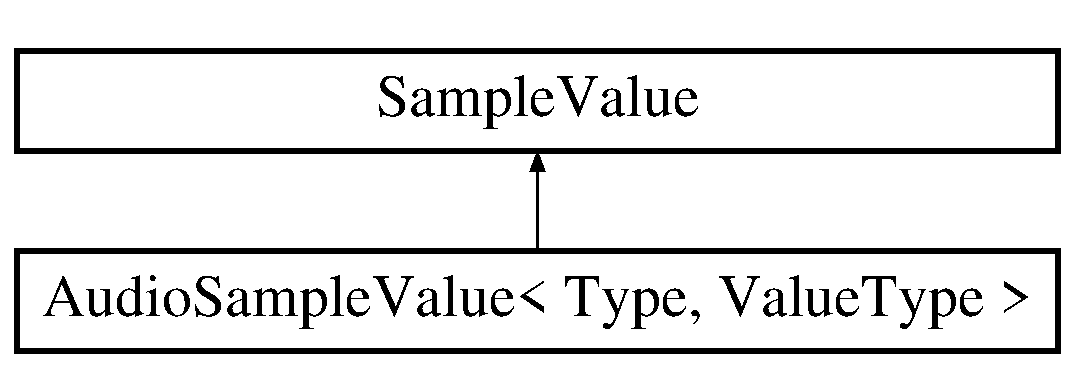
\includegraphics[height=2.000000cm]{classAudioSampleValue}
\end{center}
\end{figure}
\subsection*{Public Member Functions}
\begin{DoxyCompactItemize}
\item 
\textbf{ Audio\+Sample\+Value} (Value\+Type v)
\item 
Value\+Type \textbf{ get\+Value} (void) const
\item 
\textbf{ Sample\+Value} $\ast$ \textbf{ get\+Nearest\+Target\+Sample\+Value} (\textbf{ Emb\+Value} t) const
\item 
\textbf{ U\+W\+O\+R\+D32} \textbf{ calc\+Distance} (const \textbf{ Sample\+Value} $\ast$s) const
\item 
std\+::string \textbf{ get\+Name} (void) const
\end{DoxyCompactItemize}
\subsection*{Private Member Functions}
\begin{DoxyCompactItemize}
\item 
\textbf{ U\+W\+O\+R\+D32} \textbf{ calc\+Key} (Value\+Type v) const
\item 
\textbf{ Emb\+Value} \textbf{ calc\+E\+Value} (Value\+Type v) const
\end{DoxyCompactItemize}
\subsection*{Private Attributes}
\begin{DoxyCompactItemize}
\item 
Value\+Type \textbf{ Value}
\end{DoxyCompactItemize}
\subsection*{Static Private Attributes}
\begin{DoxyCompactItemize}
\item 
static const Value\+Type \textbf{ Min\+Value} = 0
\item 
static const Value\+Type \textbf{ Max\+Value} = \textbf{ B\+Y\+T\+E\+\_\+\+M\+AX}
\end{DoxyCompactItemize}
\subsection*{Additional Inherited Members}


\subsection{Constructor \& Destructor Documentation}
\mbox{\label{classAudioSampleValue_af6cfbcff00be2bae6f3627d6dc20dbca}} 
\index{Audio\+Sample\+Value@{Audio\+Sample\+Value}!Audio\+Sample\+Value@{Audio\+Sample\+Value}}
\index{Audio\+Sample\+Value@{Audio\+Sample\+Value}!Audio\+Sample\+Value@{Audio\+Sample\+Value}}
\subsubsection{Audio\+Sample\+Value()}
{\footnotesize\ttfamily template$<$A\+U\+D\+I\+O\+S\+A\+M\+P\+L\+E\+T\+Y\+PE Type, class Value\+Type $>$ \\
\textbf{ Audio\+Sample\+Value}$<$ Type, Value\+Type $>$\+::\textbf{ Audio\+Sample\+Value} (\begin{DoxyParamCaption}\item[{Value\+Type}]{v }\end{DoxyParamCaption})}



\subsection{Member Function Documentation}
\mbox{\label{classAudioSampleValue_a6e8bd4368a717ab9d97b0f85e3bcc24f}} 
\index{Audio\+Sample\+Value@{Audio\+Sample\+Value}!calc\+Distance@{calc\+Distance}}
\index{calc\+Distance@{calc\+Distance}!Audio\+Sample\+Value@{Audio\+Sample\+Value}}
\subsubsection{calc\+Distance()}
{\footnotesize\ttfamily template$<$A\+U\+D\+I\+O\+S\+A\+M\+P\+L\+E\+T\+Y\+PE Type, class Value\+Type $>$ \\
\textbf{ U\+W\+O\+R\+D32} \textbf{ Audio\+Sample\+Value}$<$ Type, Value\+Type $>$\+::calc\+Distance (\begin{DoxyParamCaption}\item[{const \textbf{ Sample\+Value} $\ast$}]{s }\end{DoxyParamCaption}) const\hspace{0.3cm}{\ttfamily [virtual]}}

calculate the distance between the sample value s and this sample value 
\begin{DoxyParams}{Parameters}
{\em s} & a sample value of the same type as this \\
\hline
\end{DoxyParams}
\begin{DoxyReturn}{Returns}
the distance 
\end{DoxyReturn}


Implements \textbf{ Sample\+Value} \doxyref{}{p.}{classSampleValue_aa7e5d9b69203f6f6edf97c79319232dd}.

\mbox{\label{classAudioSampleValue_afa22f9a448376232b62075c83491492e}} 
\index{Audio\+Sample\+Value@{Audio\+Sample\+Value}!calc\+E\+Value@{calc\+E\+Value}}
\index{calc\+E\+Value@{calc\+E\+Value}!Audio\+Sample\+Value@{Audio\+Sample\+Value}}
\subsubsection{calc\+E\+Value()}
{\footnotesize\ttfamily template$<$A\+U\+D\+I\+O\+S\+A\+M\+P\+L\+E\+T\+Y\+PE Type, class Value\+Type$>$ \\
\textbf{ Emb\+Value} \textbf{ Audio\+Sample\+Value}$<$ Type, Value\+Type $>$\+::calc\+E\+Value (\begin{DoxyParamCaption}\item[{Value\+Type}]{v }\end{DoxyParamCaption}) const\hspace{0.3cm}{\ttfamily [inline]}, {\ttfamily [private]}}

\mbox{\label{classAudioSampleValue_ac3110059b0db7a57585dc80691d6d4d0}} 
\index{Audio\+Sample\+Value@{Audio\+Sample\+Value}!calc\+Key@{calc\+Key}}
\index{calc\+Key@{calc\+Key}!Audio\+Sample\+Value@{Audio\+Sample\+Value}}
\subsubsection{calc\+Key()}
{\footnotesize\ttfamily template$<$A\+U\+D\+I\+O\+S\+A\+M\+P\+L\+E\+T\+Y\+PE Type, class Value\+Type$>$ \\
\textbf{ U\+W\+O\+R\+D32} \textbf{ Audio\+Sample\+Value}$<$ Type, Value\+Type $>$\+::calc\+Key (\begin{DoxyParamCaption}\item[{Value\+Type}]{v }\end{DoxyParamCaption}) const\hspace{0.3cm}{\ttfamily [inline]}, {\ttfamily [private]}}

\mbox{\label{classAudioSampleValue_a9f6d83bd0007d8a9b157f55161519b08}} 
\index{Audio\+Sample\+Value@{Audio\+Sample\+Value}!get\+Name@{get\+Name}}
\index{get\+Name@{get\+Name}!Audio\+Sample\+Value@{Audio\+Sample\+Value}}
\subsubsection{get\+Name()}
{\footnotesize\ttfamily template$<$A\+U\+D\+I\+O\+S\+A\+M\+P\+L\+E\+T\+Y\+PE Type, class Value\+Type $>$ \\
std\+::string \textbf{ Audio\+Sample\+Value}$<$ Type, Value\+Type $>$\+::get\+Name (\begin{DoxyParamCaption}\item[{void}]{ }\end{DoxyParamCaption}) const\hspace{0.3cm}{\ttfamily [virtual]}}

return a short name uniquely identifying this sample value 

Implements \textbf{ Sample\+Value} \doxyref{}{p.}{classSampleValue_aeaf5c46ec6d023840e9773604b20d25c}.

\mbox{\label{classAudioSampleValue_aaeaaef73950dbe29a1bb1620bd4c53ab}} 
\index{Audio\+Sample\+Value@{Audio\+Sample\+Value}!get\+Nearest\+Target\+Sample\+Value@{get\+Nearest\+Target\+Sample\+Value}}
\index{get\+Nearest\+Target\+Sample\+Value@{get\+Nearest\+Target\+Sample\+Value}!Audio\+Sample\+Value@{Audio\+Sample\+Value}}
\subsubsection{get\+Nearest\+Target\+Sample\+Value()}
{\footnotesize\ttfamily template$<$A\+U\+D\+I\+O\+S\+A\+M\+P\+L\+E\+T\+Y\+PE Type, class Value\+Type $>$ \\
\textbf{ Sample\+Value} $\ast$ \textbf{ Audio\+Sample\+Value}$<$ Type, Value\+Type $>$\+::get\+Nearest\+Target\+Sample\+Value (\begin{DoxyParamCaption}\item[{\textbf{ Emb\+Value}}]{t }\end{DoxyParamCaption}) const\hspace{0.3cm}{\ttfamily [virtual]}}

get the nearest (with the least distance to this sample value) sample value whose embedded value equals the specified target 
\begin{DoxyParams}{Parameters}
{\em t} & the target embedded value\\
\hline
\end{DoxyParams}
If two or more target sample values have equal distance each of them should be returned with equal probability.

The returned \doxyref{Sample\+Value}{p.}{classSampleValue} object should be deleted by the callser. 

Implements \textbf{ Sample\+Value} \doxyref{}{p.}{classSampleValue_aeca3fc1fd34c09d2244706b010935c2c}.

\mbox{\label{classAudioSampleValue_a8f050529c4f956faa8105130ea90d578}} 
\index{Audio\+Sample\+Value@{Audio\+Sample\+Value}!get\+Value@{get\+Value}}
\index{get\+Value@{get\+Value}!Audio\+Sample\+Value@{Audio\+Sample\+Value}}
\subsubsection{get\+Value()}
{\footnotesize\ttfamily template$<$A\+U\+D\+I\+O\+S\+A\+M\+P\+L\+E\+T\+Y\+PE Type, class Value\+Type$>$ \\
Value\+Type \textbf{ Audio\+Sample\+Value}$<$ Type, Value\+Type $>$\+::get\+Value (\begin{DoxyParamCaption}\item[{void}]{ }\end{DoxyParamCaption}) const\hspace{0.3cm}{\ttfamily [inline]}}



\subsection{Member Data Documentation}
\mbox{\label{classAudioSampleValue_a852909519410c701cb47ab84c25c43f5}} 
\index{Audio\+Sample\+Value@{Audio\+Sample\+Value}!Max\+Value@{Max\+Value}}
\index{Max\+Value@{Max\+Value}!Audio\+Sample\+Value@{Audio\+Sample\+Value}}
\subsubsection{Max\+Value}
{\footnotesize\ttfamily template$<$A\+U\+D\+I\+O\+S\+A\+M\+P\+L\+E\+T\+Y\+PE Type, class Value\+Type$>$ \\
const \textbf{ S\+W\+O\+R\+D32} Au\+P\+C\+M32\+Sample\+Value\+::\+Max\+Value = \textbf{ B\+Y\+T\+E\+\_\+\+M\+AX}\hspace{0.3cm}{\ttfamily [static]}, {\ttfamily [private]}}

\mbox{\label{classAudioSampleValue_ae606d07bca09850c1448720c80c002b8}} 
\index{Audio\+Sample\+Value@{Audio\+Sample\+Value}!Min\+Value@{Min\+Value}}
\index{Min\+Value@{Min\+Value}!Audio\+Sample\+Value@{Audio\+Sample\+Value}}
\subsubsection{Min\+Value}
{\footnotesize\ttfamily template$<$A\+U\+D\+I\+O\+S\+A\+M\+P\+L\+E\+T\+Y\+PE Type, class Value\+Type$>$ \\
const \textbf{ S\+W\+O\+R\+D32} Au\+P\+C\+M32\+Sample\+Value\+::\+Min\+Value = 0\hspace{0.3cm}{\ttfamily [static]}, {\ttfamily [private]}}

\mbox{\label{classAudioSampleValue_a7d800edb6ec6c2d5ccd7150cea3aab54}} 
\index{Audio\+Sample\+Value@{Audio\+Sample\+Value}!Value@{Value}}
\index{Value@{Value}!Audio\+Sample\+Value@{Audio\+Sample\+Value}}
\subsubsection{Value}
{\footnotesize\ttfamily template$<$A\+U\+D\+I\+O\+S\+A\+M\+P\+L\+E\+T\+Y\+PE Type, class Value\+Type$>$ \\
Value\+Type \textbf{ Audio\+Sample\+Value}$<$ Type, Value\+Type $>$\+::Value\hspace{0.3cm}{\ttfamily [private]}}



The documentation for this class was generated from the following files\+:\begin{DoxyCompactItemize}
\item 
\textbf{ Audio\+Sample\+Value.\+h}\item 
\textbf{ Au\+Sample\+Values.\+cc}\end{DoxyCompactItemize}

\section{Audio\+Sample\+Value\+Test Class Reference}
\label{classAudioSampleValueTest}\index{Audio\+Sample\+Value\+Test@{Audio\+Sample\+Value\+Test}}


{\ttfamily \#include $<$Audio\+Sample\+Value\+Test.\+h$>$}

Inheritance diagram for Audio\+Sample\+Value\+Test\+:\begin{figure}[H]
\begin{center}
\leavevmode
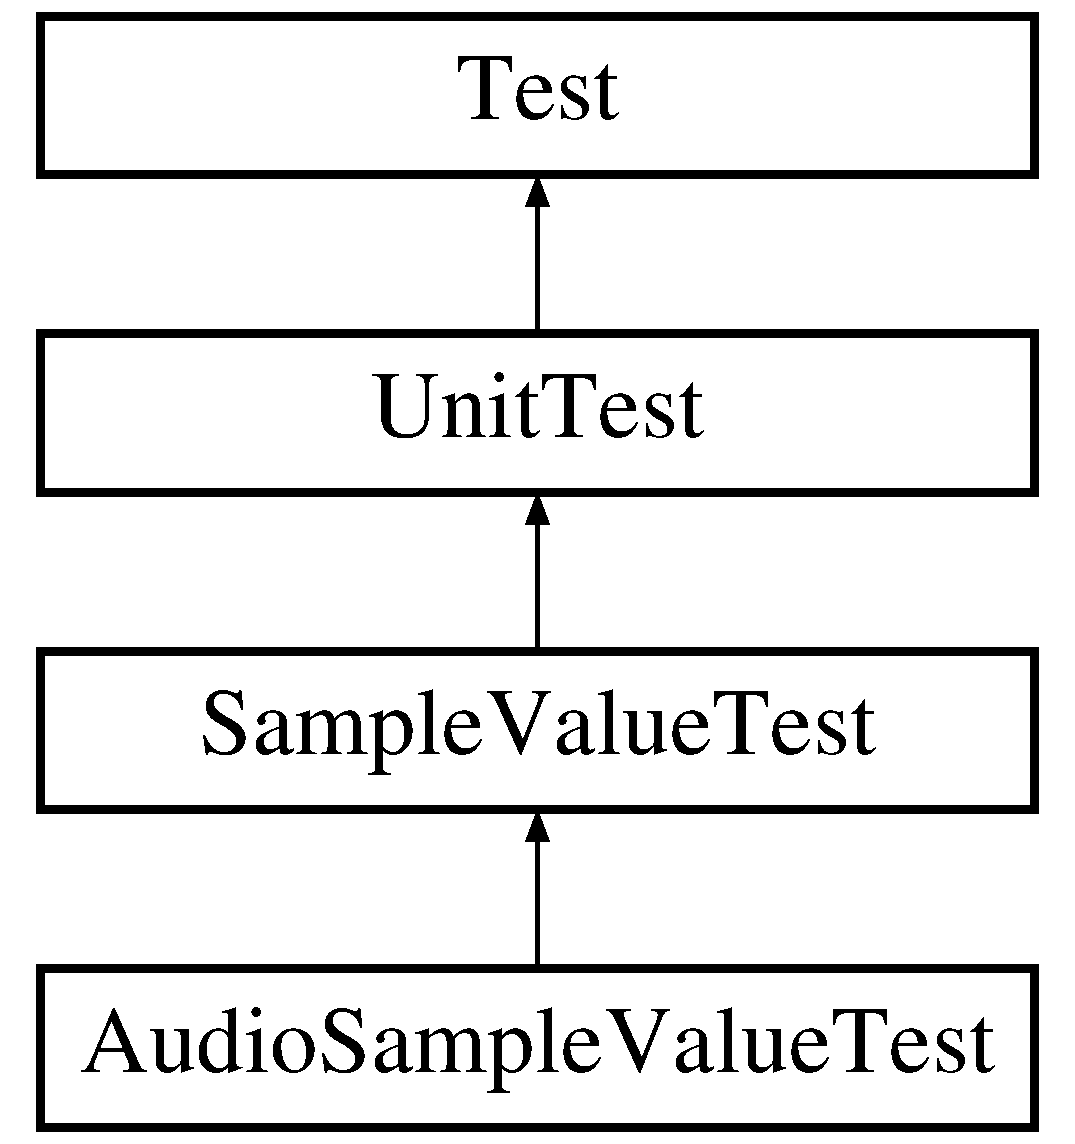
\includegraphics[height=4.000000cm]{classAudioSampleValueTest}
\end{center}
\end{figure}
\subsection*{Public Member Functions}
\begin{DoxyCompactItemize}
\item 
\textbf{ Audio\+Sample\+Value\+Test} (\textbf{ Test\+Suite} $\ast$s)
\item 
void \textbf{ setup} (void)
\item 
void \textbf{ cleanup} (void)
\item 
void \textbf{ test\+Distance} (void)
\item 
void \textbf{ test\+Is\+Neighbour} (void)
\end{DoxyCompactItemize}
\subsection*{Private Attributes}
\begin{DoxyCompactItemize}
\item 
\textbf{ Cvr\+Stg\+File} $\ast$ \textbf{ f\+\_\+\+Au\+Mu\+Law}
\item 
\textbf{ Cvr\+Stg\+File} $\ast$ \textbf{ f\+\_\+\+Au\+P\+C\+M16}
\item 
\textbf{ Sample\+Value} $\ast$ \textbf{ sv\+\_\+\+Au\+Mu\+Law\+\_\+0}
\item 
\textbf{ Sample\+Value} $\ast$ \textbf{ sv\+\_\+\+Au\+Mu\+Law\+\_\+1}
\item 
\textbf{ Sample\+Value} $\ast$ \textbf{ sv\+\_\+\+Au\+Mu\+Law\+\_\+45}
\item 
\textbf{ Sample\+Value} $\ast$ \textbf{ sv\+\_\+\+Au\+P\+C\+M16\+\_\+m32768}
\item 
\textbf{ Sample\+Value} $\ast$ \textbf{ sv\+\_\+\+Au\+P\+C\+M16\+\_\+32767}
\item 
\textbf{ Sample\+Value} $\ast$ \textbf{ sv\+\_\+\+Au\+P\+C\+M16\+\_\+0}
\item 
\textbf{ Sample\+Value} $\ast$ \textbf{ sv\+\_\+\+Au\+P\+C\+M16\+\_\+15}
\item 
\textbf{ Globals} \textbf{ gl\+\_\+\+Au\+Mu\+Law}
\item 
\textbf{ Globals} \textbf{ gl\+\_\+\+Au\+P\+C\+M16}
\end{DoxyCompactItemize}
\subsection*{Additional Inherited Members}


\subsection{Constructor \& Destructor Documentation}
\mbox{\label{classAudioSampleValueTest_a86807bf88f51993acd72fd2a7e772068}} 
\index{Audio\+Sample\+Value\+Test@{Audio\+Sample\+Value\+Test}!Audio\+Sample\+Value\+Test@{Audio\+Sample\+Value\+Test}}
\index{Audio\+Sample\+Value\+Test@{Audio\+Sample\+Value\+Test}!Audio\+Sample\+Value\+Test@{Audio\+Sample\+Value\+Test}}
\subsubsection{Audio\+Sample\+Value\+Test()}
{\footnotesize\ttfamily Audio\+Sample\+Value\+Test\+::\+Audio\+Sample\+Value\+Test (\begin{DoxyParamCaption}\item[{\textbf{ Test\+Suite} $\ast$}]{s }\end{DoxyParamCaption})}



\subsection{Member Function Documentation}
\mbox{\label{classAudioSampleValueTest_a9c89c4e4802bc59647e95d8323d8c0bb}} 
\index{Audio\+Sample\+Value\+Test@{Audio\+Sample\+Value\+Test}!cleanup@{cleanup}}
\index{cleanup@{cleanup}!Audio\+Sample\+Value\+Test@{Audio\+Sample\+Value\+Test}}
\subsubsection{cleanup()}
{\footnotesize\ttfamily void Audio\+Sample\+Value\+Test\+::cleanup (\begin{DoxyParamCaption}\item[{void}]{ }\end{DoxyParamCaption})\hspace{0.3cm}{\ttfamily [virtual]}}

cleanup the unit test -\/ called after run 

Reimplemented from \textbf{ Unit\+Test} \doxyref{}{p.}{classUnitTest_adf77efe972ee4a766d94e3f7ddc193ad}.

\mbox{\label{classAudioSampleValueTest_a82fa9023cfe5cdf9891138928a059b46}} 
\index{Audio\+Sample\+Value\+Test@{Audio\+Sample\+Value\+Test}!setup@{setup}}
\index{setup@{setup}!Audio\+Sample\+Value\+Test@{Audio\+Sample\+Value\+Test}}
\subsubsection{setup()}
{\footnotesize\ttfamily void Audio\+Sample\+Value\+Test\+::setup (\begin{DoxyParamCaption}\item[{void}]{ }\end{DoxyParamCaption})\hspace{0.3cm}{\ttfamily [virtual]}}

setup the unit test -\/ called before run

\doxyref{Unit\+Test\+::setup}{p.}{classUnitTest_ad73fdf9012b651047ea001d21f9d27ad} will (together with \doxyref{Unit\+Test\+::cleanup}{p.}{classUnitTest_adf77efe972ee4a766d94e3f7ddc193ad}) save and restore the object stored in Globs so they should be called from the corresponding functions in the derived object if the derived unit test manipulates the Globs object. 

Reimplemented from \textbf{ Unit\+Test} \doxyref{}{p.}{classUnitTest_ad73fdf9012b651047ea001d21f9d27ad}.

\mbox{\label{classAudioSampleValueTest_a6468aea3e12179711b02daa33b79bb04}} 
\index{Audio\+Sample\+Value\+Test@{Audio\+Sample\+Value\+Test}!test\+Distance@{test\+Distance}}
\index{test\+Distance@{test\+Distance}!Audio\+Sample\+Value\+Test@{Audio\+Sample\+Value\+Test}}
\subsubsection{test\+Distance()}
{\footnotesize\ttfamily void Audio\+Sample\+Value\+Test\+::test\+Distance (\begin{DoxyParamCaption}\item[{void}]{ }\end{DoxyParamCaption})}

\mbox{\label{classAudioSampleValueTest_a638623e053accab88a6ec908104dd4fa}} 
\index{Audio\+Sample\+Value\+Test@{Audio\+Sample\+Value\+Test}!test\+Is\+Neighbour@{test\+Is\+Neighbour}}
\index{test\+Is\+Neighbour@{test\+Is\+Neighbour}!Audio\+Sample\+Value\+Test@{Audio\+Sample\+Value\+Test}}
\subsubsection{test\+Is\+Neighbour()}
{\footnotesize\ttfamily void Audio\+Sample\+Value\+Test\+::test\+Is\+Neighbour (\begin{DoxyParamCaption}\item[{void}]{ }\end{DoxyParamCaption})}



\subsection{Member Data Documentation}
\mbox{\label{classAudioSampleValueTest_a7aead14c08dd9c12e8ce730f06037f83}} 
\index{Audio\+Sample\+Value\+Test@{Audio\+Sample\+Value\+Test}!f\+\_\+\+Au\+Mu\+Law@{f\+\_\+\+Au\+Mu\+Law}}
\index{f\+\_\+\+Au\+Mu\+Law@{f\+\_\+\+Au\+Mu\+Law}!Audio\+Sample\+Value\+Test@{Audio\+Sample\+Value\+Test}}
\subsubsection{f\+\_\+\+Au\+Mu\+Law}
{\footnotesize\ttfamily \textbf{ Cvr\+Stg\+File}$\ast$ Audio\+Sample\+Value\+Test\+::f\+\_\+\+Au\+Mu\+Law\hspace{0.3cm}{\ttfamily [private]}}

\mbox{\label{classAudioSampleValueTest_a35c3dabeeba9e5a829f16d2545bba70c}} 
\index{Audio\+Sample\+Value\+Test@{Audio\+Sample\+Value\+Test}!f\+\_\+\+Au\+P\+C\+M16@{f\+\_\+\+Au\+P\+C\+M16}}
\index{f\+\_\+\+Au\+P\+C\+M16@{f\+\_\+\+Au\+P\+C\+M16}!Audio\+Sample\+Value\+Test@{Audio\+Sample\+Value\+Test}}
\subsubsection{f\+\_\+\+Au\+P\+C\+M16}
{\footnotesize\ttfamily \textbf{ Cvr\+Stg\+File} $\ast$ Audio\+Sample\+Value\+Test\+::f\+\_\+\+Au\+P\+C\+M16\hspace{0.3cm}{\ttfamily [private]}}

\mbox{\label{classAudioSampleValueTest_af2a96fc157b19ddde86614007990eab7}} 
\index{Audio\+Sample\+Value\+Test@{Audio\+Sample\+Value\+Test}!gl\+\_\+\+Au\+Mu\+Law@{gl\+\_\+\+Au\+Mu\+Law}}
\index{gl\+\_\+\+Au\+Mu\+Law@{gl\+\_\+\+Au\+Mu\+Law}!Audio\+Sample\+Value\+Test@{Audio\+Sample\+Value\+Test}}
\subsubsection{gl\+\_\+\+Au\+Mu\+Law}
{\footnotesize\ttfamily \textbf{ Globals} Audio\+Sample\+Value\+Test\+::gl\+\_\+\+Au\+Mu\+Law\hspace{0.3cm}{\ttfamily [private]}}

\mbox{\label{classAudioSampleValueTest_a89c291a888d45134850d04917f44d583}} 
\index{Audio\+Sample\+Value\+Test@{Audio\+Sample\+Value\+Test}!gl\+\_\+\+Au\+P\+C\+M16@{gl\+\_\+\+Au\+P\+C\+M16}}
\index{gl\+\_\+\+Au\+P\+C\+M16@{gl\+\_\+\+Au\+P\+C\+M16}!Audio\+Sample\+Value\+Test@{Audio\+Sample\+Value\+Test}}
\subsubsection{gl\+\_\+\+Au\+P\+C\+M16}
{\footnotesize\ttfamily \textbf{ Globals} Audio\+Sample\+Value\+Test\+::gl\+\_\+\+Au\+P\+C\+M16\hspace{0.3cm}{\ttfamily [private]}}

\mbox{\label{classAudioSampleValueTest_a2b99b1abf6b03aedcbea95b9ae7594ff}} 
\index{Audio\+Sample\+Value\+Test@{Audio\+Sample\+Value\+Test}!sv\+\_\+\+Au\+Mu\+Law\+\_\+0@{sv\+\_\+\+Au\+Mu\+Law\+\_\+0}}
\index{sv\+\_\+\+Au\+Mu\+Law\+\_\+0@{sv\+\_\+\+Au\+Mu\+Law\+\_\+0}!Audio\+Sample\+Value\+Test@{Audio\+Sample\+Value\+Test}}
\subsubsection{sv\+\_\+\+Au\+Mu\+Law\+\_\+0}
{\footnotesize\ttfamily \textbf{ Sample\+Value}$\ast$ Audio\+Sample\+Value\+Test\+::sv\+\_\+\+Au\+Mu\+Law\+\_\+0\hspace{0.3cm}{\ttfamily [private]}}

\mbox{\label{classAudioSampleValueTest_a6f92285bea82219b0bf90715448deb8a}} 
\index{Audio\+Sample\+Value\+Test@{Audio\+Sample\+Value\+Test}!sv\+\_\+\+Au\+Mu\+Law\+\_\+1@{sv\+\_\+\+Au\+Mu\+Law\+\_\+1}}
\index{sv\+\_\+\+Au\+Mu\+Law\+\_\+1@{sv\+\_\+\+Au\+Mu\+Law\+\_\+1}!Audio\+Sample\+Value\+Test@{Audio\+Sample\+Value\+Test}}
\subsubsection{sv\+\_\+\+Au\+Mu\+Law\+\_\+1}
{\footnotesize\ttfamily \textbf{ Sample\+Value} $\ast$ Audio\+Sample\+Value\+Test\+::sv\+\_\+\+Au\+Mu\+Law\+\_\+1\hspace{0.3cm}{\ttfamily [private]}}

\mbox{\label{classAudioSampleValueTest_a867914d4413297bf87a70ad3c4c2794b}} 
\index{Audio\+Sample\+Value\+Test@{Audio\+Sample\+Value\+Test}!sv\+\_\+\+Au\+Mu\+Law\+\_\+45@{sv\+\_\+\+Au\+Mu\+Law\+\_\+45}}
\index{sv\+\_\+\+Au\+Mu\+Law\+\_\+45@{sv\+\_\+\+Au\+Mu\+Law\+\_\+45}!Audio\+Sample\+Value\+Test@{Audio\+Sample\+Value\+Test}}
\subsubsection{sv\+\_\+\+Au\+Mu\+Law\+\_\+45}
{\footnotesize\ttfamily \textbf{ Sample\+Value} $\ast$ Audio\+Sample\+Value\+Test\+::sv\+\_\+\+Au\+Mu\+Law\+\_\+45\hspace{0.3cm}{\ttfamily [private]}}

\mbox{\label{classAudioSampleValueTest_a1a5e12e19eb20ee9a51d5cba84369389}} 
\index{Audio\+Sample\+Value\+Test@{Audio\+Sample\+Value\+Test}!sv\+\_\+\+Au\+P\+C\+M16\+\_\+0@{sv\+\_\+\+Au\+P\+C\+M16\+\_\+0}}
\index{sv\+\_\+\+Au\+P\+C\+M16\+\_\+0@{sv\+\_\+\+Au\+P\+C\+M16\+\_\+0}!Audio\+Sample\+Value\+Test@{Audio\+Sample\+Value\+Test}}
\subsubsection{sv\+\_\+\+Au\+P\+C\+M16\+\_\+0}
{\footnotesize\ttfamily \textbf{ Sample\+Value} $\ast$ Audio\+Sample\+Value\+Test\+::sv\+\_\+\+Au\+P\+C\+M16\+\_\+0\hspace{0.3cm}{\ttfamily [private]}}

\mbox{\label{classAudioSampleValueTest_a30ac18f7729ae55fa4a850b6c2aa4ff9}} 
\index{Audio\+Sample\+Value\+Test@{Audio\+Sample\+Value\+Test}!sv\+\_\+\+Au\+P\+C\+M16\+\_\+15@{sv\+\_\+\+Au\+P\+C\+M16\+\_\+15}}
\index{sv\+\_\+\+Au\+P\+C\+M16\+\_\+15@{sv\+\_\+\+Au\+P\+C\+M16\+\_\+15}!Audio\+Sample\+Value\+Test@{Audio\+Sample\+Value\+Test}}
\subsubsection{sv\+\_\+\+Au\+P\+C\+M16\+\_\+15}
{\footnotesize\ttfamily \textbf{ Sample\+Value} $\ast$ Audio\+Sample\+Value\+Test\+::sv\+\_\+\+Au\+P\+C\+M16\+\_\+15\hspace{0.3cm}{\ttfamily [private]}}

\mbox{\label{classAudioSampleValueTest_a99081a4b596954509b7aed5333330143}} 
\index{Audio\+Sample\+Value\+Test@{Audio\+Sample\+Value\+Test}!sv\+\_\+\+Au\+P\+C\+M16\+\_\+32767@{sv\+\_\+\+Au\+P\+C\+M16\+\_\+32767}}
\index{sv\+\_\+\+Au\+P\+C\+M16\+\_\+32767@{sv\+\_\+\+Au\+P\+C\+M16\+\_\+32767}!Audio\+Sample\+Value\+Test@{Audio\+Sample\+Value\+Test}}
\subsubsection{sv\+\_\+\+Au\+P\+C\+M16\+\_\+32767}
{\footnotesize\ttfamily \textbf{ Sample\+Value} $\ast$ Audio\+Sample\+Value\+Test\+::sv\+\_\+\+Au\+P\+C\+M16\+\_\+32767\hspace{0.3cm}{\ttfamily [private]}}

\mbox{\label{classAudioSampleValueTest_ab57022a8527a973a2ee02439254f9c40}} 
\index{Audio\+Sample\+Value\+Test@{Audio\+Sample\+Value\+Test}!sv\+\_\+\+Au\+P\+C\+M16\+\_\+m32768@{sv\+\_\+\+Au\+P\+C\+M16\+\_\+m32768}}
\index{sv\+\_\+\+Au\+P\+C\+M16\+\_\+m32768@{sv\+\_\+\+Au\+P\+C\+M16\+\_\+m32768}!Audio\+Sample\+Value\+Test@{Audio\+Sample\+Value\+Test}}
\subsubsection{sv\+\_\+\+Au\+P\+C\+M16\+\_\+m32768}
{\footnotesize\ttfamily \textbf{ Sample\+Value} $\ast$ Audio\+Sample\+Value\+Test\+::sv\+\_\+\+Au\+P\+C\+M16\+\_\+m32768\hspace{0.3cm}{\ttfamily [private]}}



The documentation for this class was generated from the following files\+:\begin{DoxyCompactItemize}
\item 
\textbf{ Audio\+Sample\+Value\+Test.\+h}\item 
\textbf{ Audio\+Sample\+Value\+Test.\+cc}\end{DoxyCompactItemize}

\section{Au\+File Class Reference}
\label{classAuFile}\index{Au\+File@{Au\+File}}


a \doxyref{Cvr\+Stg\+File}{p.}{classCvrStgFile} in Sun .au format  




{\ttfamily \#include $<$Au\+File.\+h$>$}

Inheritance diagram for Au\+File\+:\begin{figure}[H]
\begin{center}
\leavevmode
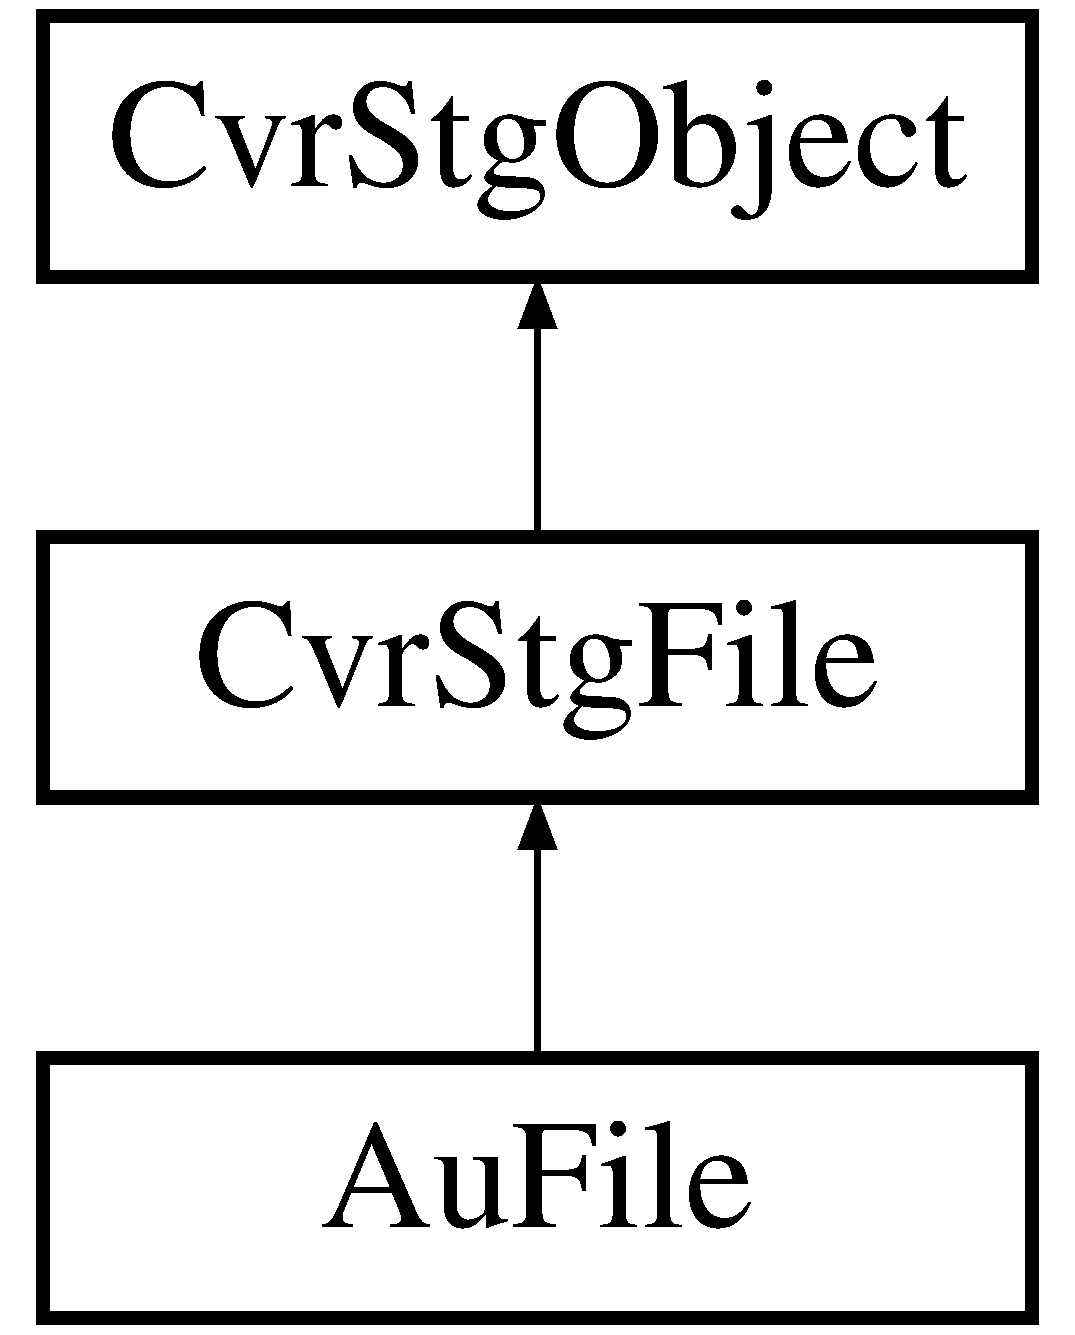
\includegraphics[height=3.000000cm]{classAuFile}
\end{center}
\end{figure}
\subsection*{Classes}
\begin{DoxyCompactItemize}
\item 
class \textbf{ Au\+Header}
\end{DoxyCompactItemize}
\subsection*{Public Member Functions}
\begin{DoxyCompactItemize}
\item 
\textbf{ Au\+File} (\textbf{ Binary\+IO} $\ast$io)
\item 
\textbf{ $\sim$\+Au\+File} (void)
\item 
void \textbf{ read} (\textbf{ Binary\+IO} $\ast$io)
\item 
void \textbf{ write} (void)
\item 
std\+::list$<$ \textbf{ Cvr\+Stg\+File\+::\+Property} $>$ \textbf{ get\+Properties} (void) const
\item 
std\+::vector$<$ \textbf{ Matching\+Algorithm} $\ast$ $>$ \textbf{ get\+Matching\+Algorithms} (\textbf{ Graph} $\ast$g, \textbf{ Matching} $\ast$m) const
\item 
unsigned long \textbf{ get\+Num\+Samples} (void) const
\item 
void \textbf{ replace\+Sample} (const \textbf{ Sample\+Pos} pos, const \textbf{ Sample\+Value} $\ast$s)
\item 
\textbf{ Sample\+Value} $\ast$ \textbf{ get\+Sample\+Value} (\textbf{ Sample\+Pos} pos) const
\end{DoxyCompactItemize}
\subsection*{Private Types}
\begin{DoxyCompactItemize}
\item 
enum \textbf{ E\+N\+C\+O\+D\+I\+NG} \{ \textbf{ M\+U\+L\+A\+W8} = 1, 
\textbf{ P\+C\+M8} = 2, 
\textbf{ P\+C\+M16} = 3
 \}
\end{DoxyCompactItemize}
\subsection*{Private Attributes}
\begin{DoxyCompactItemize}
\item 
\textbf{ Au\+Header} \textbf{ Header}
\item 
std\+::vector$<$ \textbf{ B\+Y\+TE} $>$ \textbf{ Infofield}
\item 
\textbf{ Audio\+Data} $\ast$ \textbf{ Data}
\end{DoxyCompactItemize}
\subsection*{Static Private Attributes}
\begin{DoxyCompactItemize}
\item 
static const \textbf{ U\+W\+O\+R\+D32} \textbf{ Radius\+\_\+\+Mu\+Law8} = 1
\item 
static const \textbf{ U\+W\+O\+R\+D32} \textbf{ Radius\+\_\+\+P\+C\+M8} = 1
\item 
static const \textbf{ U\+W\+O\+R\+D32} \textbf{ Radius\+\_\+\+P\+C\+M16} = 20
\item 
static const unsigned short \textbf{ Samples\+Per\+Vertex} = 2
\item 
static const \textbf{ Emb\+Value} \textbf{ Emb\+Value\+Modulus} = 2
\end{DoxyCompactItemize}
\subsection*{Additional Inherited Members}


\subsection{Member Enumeration Documentation}
\mbox{\label{classAuFile_a24effbfb64f3b6055dac14ac4fe3c485}} 
\index{Au\+File@{Au\+File}!E\+N\+C\+O\+D\+I\+NG@{E\+N\+C\+O\+D\+I\+NG}}
\index{E\+N\+C\+O\+D\+I\+NG@{E\+N\+C\+O\+D\+I\+NG}!Au\+File@{Au\+File}}
\subsubsection{E\+N\+C\+O\+D\+I\+NG}
{\footnotesize\ttfamily enum \textbf{ Au\+File\+::\+E\+N\+C\+O\+D\+I\+NG}\hspace{0.3cm}{\ttfamily [private]}}

\begin{DoxyEnumFields}{Enumerator}
\raisebox{\heightof{T}}[0pt][0pt]{\index{M\+U\+L\+A\+W8@{M\+U\+L\+A\+W8}!Au\+File@{Au\+File}}\index{Au\+File@{Au\+File}!M\+U\+L\+A\+W8@{M\+U\+L\+A\+W8}}}\mbox{\label{classAuFile_a24effbfb64f3b6055dac14ac4fe3c485ac0d7b008c7b619f982e2684fc12a5492}} 
M\+U\+L\+A\+W8&\\
\hline

\raisebox{\heightof{T}}[0pt][0pt]{\index{P\+C\+M8@{P\+C\+M8}!Au\+File@{Au\+File}}\index{Au\+File@{Au\+File}!P\+C\+M8@{P\+C\+M8}}}\mbox{\label{classAuFile_a24effbfb64f3b6055dac14ac4fe3c485a9883bf7380667e38228a2c7c953ba49a}} 
P\+C\+M8&\\
\hline

\raisebox{\heightof{T}}[0pt][0pt]{\index{P\+C\+M16@{P\+C\+M16}!Au\+File@{Au\+File}}\index{Au\+File@{Au\+File}!P\+C\+M16@{P\+C\+M16}}}\mbox{\label{classAuFile_a24effbfb64f3b6055dac14ac4fe3c485a5ad0d2903b59e209eed1c88c65f573b0}} 
P\+C\+M16&\\
\hline

\end{DoxyEnumFields}


\subsection{Constructor \& Destructor Documentation}
\mbox{\label{classAuFile_a8d4adaac11d68ee333c78ef02e4d97eb}} 
\index{Au\+File@{Au\+File}!Au\+File@{Au\+File}}
\index{Au\+File@{Au\+File}!Au\+File@{Au\+File}}
\subsubsection{Au\+File()}
{\footnotesize\ttfamily Au\+File\+::\+Au\+File (\begin{DoxyParamCaption}\item[{\textbf{ Binary\+IO} $\ast$}]{io }\end{DoxyParamCaption})}

\mbox{\label{classAuFile_a7c1b9777c3e1e951788ae814d418ef3a}} 
\index{Au\+File@{Au\+File}!````~Au\+File@{$\sim$\+Au\+File}}
\index{````~Au\+File@{$\sim$\+Au\+File}!Au\+File@{Au\+File}}
\subsubsection{$\sim$\+Au\+File()}
{\footnotesize\ttfamily Au\+File\+::$\sim$\+Au\+File (\begin{DoxyParamCaption}\item[{void}]{ }\end{DoxyParamCaption})}



\subsection{Member Function Documentation}
\mbox{\label{classAuFile_adce884ef9a8ba89ffb69dc03bf0a10ae}} 
\index{Au\+File@{Au\+File}!get\+Matching\+Algorithms@{get\+Matching\+Algorithms}}
\index{get\+Matching\+Algorithms@{get\+Matching\+Algorithms}!Au\+File@{Au\+File}}
\subsubsection{get\+Matching\+Algorithms()}
{\footnotesize\ttfamily std\+::vector$<$ \textbf{ Matching\+Algorithm} $\ast$ $>$ Au\+File\+::get\+Matching\+Algorithms (\begin{DoxyParamCaption}\item[{\textbf{ Graph} $\ast$}]{g,  }\item[{\textbf{ Matching} $\ast$}]{m }\end{DoxyParamCaption}) const\hspace{0.3cm}{\ttfamily [virtual]}}

get recommended list of matching algorithms 
\begin{DoxyParams}{Parameters}
{\em m} & an empty matching -\/ will be used in construction of \doxyref{Matching\+Algorithm}{p.}{classMatchingAlgorithm} objects\\
\hline
\end{DoxyParams}
The \doxyref{Matching\+Algorithm}{p.}{classMatchingAlgorithm} objects returned by this function should be deleted by the caller if they are no longer needed. 

Reimplemented from \textbf{ Cvr\+Stg\+File} \doxyref{}{p.}{classCvrStgFile_aa0b1087f94e191b72e794a56e49bb706}.

\mbox{\label{classAuFile_a6207c3612049d7467805842de926934e}} 
\index{Au\+File@{Au\+File}!get\+Num\+Samples@{get\+Num\+Samples}}
\index{get\+Num\+Samples@{get\+Num\+Samples}!Au\+File@{Au\+File}}
\subsubsection{get\+Num\+Samples()}
{\footnotesize\ttfamily unsigned long Au\+File\+::get\+Num\+Samples (\begin{DoxyParamCaption}\item[{void}]{ }\end{DoxyParamCaption}) const\hspace{0.3cm}{\ttfamily [inline]}, {\ttfamily [virtual]}}

get the number of samples in this \doxyref{Cvr\+Stg\+Object}{p.}{classCvrStgObject} 

Implements \textbf{ Cvr\+Stg\+Object} \doxyref{}{p.}{classCvrStgObject_a80ae8f095b66683e5207adf8ff8265b4}.

\mbox{\label{classAuFile_ad2953eec58ebadf95c105d5c907d09d4}} 
\index{Au\+File@{Au\+File}!get\+Properties@{get\+Properties}}
\index{get\+Properties@{get\+Properties}!Au\+File@{Au\+File}}
\subsubsection{get\+Properties()}
{\footnotesize\ttfamily std\+::list$<$ \textbf{ Cvr\+Stg\+File\+::\+Property} $>$ Au\+File\+::get\+Properties (\begin{DoxyParamCaption}\item[{void}]{ }\end{DoxyParamCaption}) const\hspace{0.3cm}{\ttfamily [virtual]}}



Implements \textbf{ Cvr\+Stg\+File} \doxyref{}{p.}{classCvrStgFile_afe2f570ea6447c0636093b44ff7793cc}.

\mbox{\label{classAuFile_af55279548dc9840e46115f859dbac36d}} 
\index{Au\+File@{Au\+File}!get\+Sample\+Value@{get\+Sample\+Value}}
\index{get\+Sample\+Value@{get\+Sample\+Value}!Au\+File@{Au\+File}}
\subsubsection{get\+Sample\+Value()}
{\footnotesize\ttfamily \textbf{ Sample\+Value}$\ast$ Au\+File\+::get\+Sample\+Value (\begin{DoxyParamCaption}\item[{\textbf{ Sample\+Pos}}]{pos }\end{DoxyParamCaption}) const\hspace{0.3cm}{\ttfamily [inline]}, {\ttfamily [virtual]}}

get the sample at position pos 
\begin{DoxyParams}{Parameters}
{\em pos} & the position of a sample (must be in 0...\doxyref{get\+Num\+Samples()}{p.}{classAuFile_a6207c3612049d7467805842de926934e}-\/1) \\
\hline
\end{DoxyParams}
\begin{DoxyReturn}{Returns}
the sample at the given position
\end{DoxyReturn}
The sample object is created in this function and should be deleted by the caller. The derived class should check the condition(s) given above in its Implementation of this function. 

Implements \textbf{ Cvr\+Stg\+Object} \doxyref{}{p.}{classCvrStgObject_ac77a8da85a4f7b53e2166e990dfaa4f2}.

\mbox{\label{classAuFile_a16b076fd6c452cd93170027f4cf42581}} 
\index{Au\+File@{Au\+File}!read@{read}}
\index{read@{read}!Au\+File@{Au\+File}}
\subsubsection{read()}
{\footnotesize\ttfamily void Au\+File\+::read (\begin{DoxyParamCaption}\item[{\textbf{ Binary\+IO} $\ast$}]{io }\end{DoxyParamCaption})\hspace{0.3cm}{\ttfamily [virtual]}}



Reimplemented from \textbf{ Cvr\+Stg\+File} \doxyref{}{p.}{classCvrStgFile_a8a568ccb2ad5d6c178f764dca6090908}.

\mbox{\label{classAuFile_a174651b1eb09ce6499dd9b49740e0585}} 
\index{Au\+File@{Au\+File}!replace\+Sample@{replace\+Sample}}
\index{replace\+Sample@{replace\+Sample}!Au\+File@{Au\+File}}
\subsubsection{replace\+Sample()}
{\footnotesize\ttfamily void Au\+File\+::replace\+Sample (\begin{DoxyParamCaption}\item[{const \textbf{ Sample\+Pos}}]{pos,  }\item[{const \textbf{ Sample\+Value} $\ast$}]{s }\end{DoxyParamCaption})\hspace{0.3cm}{\ttfamily [inline]}, {\ttfamily [virtual]}}

replace a sample thus (possibly) altering the value of the bit returned by Sample\+Value-\/$>$get\+Bit() 
\begin{DoxyParams}{Parameters}
{\em pos} & the position of the sample (must be in 0...\doxyref{get\+Num\+Samples()}{p.}{classAuFile_a6207c3612049d7467805842de926934e}-\/1) \\
\hline
{\em s} & the sample value that should replace the current sample value (must be of correct type for this \doxyref{Cvr\+Stg\+Object}{p.}{classCvrStgObject})\\
\hline
\end{DoxyParams}
The derived class should check the condition(s) given above in its Implementation of this function. 

Implements \textbf{ Cvr\+Stg\+Object} \doxyref{}{p.}{classCvrStgObject_a3068d6a9dcc1c0b8bde2f081cfde6ce5}.

\mbox{\label{classAuFile_a563b078d7d1660fdd2ebe005eb2c26c6}} 
\index{Au\+File@{Au\+File}!write@{write}}
\index{write@{write}!Au\+File@{Au\+File}}
\subsubsection{write()}
{\footnotesize\ttfamily void Au\+File\+::write (\begin{DoxyParamCaption}\item[{void}]{ }\end{DoxyParamCaption})\hspace{0.3cm}{\ttfamily [virtual]}}



Reimplemented from \textbf{ Cvr\+Stg\+File} \doxyref{}{p.}{classCvrStgFile_af2b8f47f83f9210409af6be7d750a841}.



\subsection{Member Data Documentation}
\mbox{\label{classAuFile_a7943587c3dc294e0b3a3a081fffc9940}} 
\index{Au\+File@{Au\+File}!Data@{Data}}
\index{Data@{Data}!Au\+File@{Au\+File}}
\subsubsection{Data}
{\footnotesize\ttfamily \textbf{ Audio\+Data}$\ast$ Au\+File\+::\+Data\hspace{0.3cm}{\ttfamily [private]}}

\mbox{\label{classAuFile_ad1a55c4ad3f2f2a89af01392ed482fb5}} 
\index{Au\+File@{Au\+File}!Emb\+Value\+Modulus@{Emb\+Value\+Modulus}}
\index{Emb\+Value\+Modulus@{Emb\+Value\+Modulus}!Au\+File@{Au\+File}}
\subsubsection{Emb\+Value\+Modulus}
{\footnotesize\ttfamily const \textbf{ Emb\+Value} Au\+File\+::\+Emb\+Value\+Modulus = 2\hspace{0.3cm}{\ttfamily [static]}, {\ttfamily [private]}}

\mbox{\label{classAuFile_a644fd49d94b0cb2c446dfa1c3f1b8765}} 
\index{Au\+File@{Au\+File}!Header@{Header}}
\index{Header@{Header}!Au\+File@{Au\+File}}
\subsubsection{Header}
{\footnotesize\ttfamily \textbf{ Au\+Header} Au\+File\+::\+Header\hspace{0.3cm}{\ttfamily [private]}}

\mbox{\label{classAuFile_ad85e7d37e7d0c9289eba5892d9a7400d}} 
\index{Au\+File@{Au\+File}!Infofield@{Infofield}}
\index{Infofield@{Infofield}!Au\+File@{Au\+File}}
\subsubsection{Infofield}
{\footnotesize\ttfamily std\+::vector$<$\textbf{ B\+Y\+TE}$>$ Au\+File\+::\+Infofield\hspace{0.3cm}{\ttfamily [private]}}

\mbox{\label{classAuFile_afbfdbb7c5acee758c90226547cd29832}} 
\index{Au\+File@{Au\+File}!Radius\+\_\+\+Mu\+Law8@{Radius\+\_\+\+Mu\+Law8}}
\index{Radius\+\_\+\+Mu\+Law8@{Radius\+\_\+\+Mu\+Law8}!Au\+File@{Au\+File}}
\subsubsection{Radius\+\_\+\+Mu\+Law8}
{\footnotesize\ttfamily const \textbf{ U\+W\+O\+R\+D32} Au\+File\+::\+Radius\+\_\+\+Mu\+Law8 = 1\hspace{0.3cm}{\ttfamily [static]}, {\ttfamily [private]}}

\mbox{\label{classAuFile_a960d9eccdc793d037bbce748d63456b6}} 
\index{Au\+File@{Au\+File}!Radius\+\_\+\+P\+C\+M16@{Radius\+\_\+\+P\+C\+M16}}
\index{Radius\+\_\+\+P\+C\+M16@{Radius\+\_\+\+P\+C\+M16}!Au\+File@{Au\+File}}
\subsubsection{Radius\+\_\+\+P\+C\+M16}
{\footnotesize\ttfamily const \textbf{ U\+W\+O\+R\+D32} Au\+File\+::\+Radius\+\_\+\+P\+C\+M16 = 20\hspace{0.3cm}{\ttfamily [static]}, {\ttfamily [private]}}

\mbox{\label{classAuFile_a1e2854d94a307343f2460bca656a2440}} 
\index{Au\+File@{Au\+File}!Radius\+\_\+\+P\+C\+M8@{Radius\+\_\+\+P\+C\+M8}}
\index{Radius\+\_\+\+P\+C\+M8@{Radius\+\_\+\+P\+C\+M8}!Au\+File@{Au\+File}}
\subsubsection{Radius\+\_\+\+P\+C\+M8}
{\footnotesize\ttfamily const \textbf{ U\+W\+O\+R\+D32} Au\+File\+::\+Radius\+\_\+\+P\+C\+M8 = 1\hspace{0.3cm}{\ttfamily [static]}, {\ttfamily [private]}}

\mbox{\label{classAuFile_a1bc354e94ccacb4415d4501a83481ccd}} 
\index{Au\+File@{Au\+File}!Samples\+Per\+Vertex@{Samples\+Per\+Vertex}}
\index{Samples\+Per\+Vertex@{Samples\+Per\+Vertex}!Au\+File@{Au\+File}}
\subsubsection{Samples\+Per\+Vertex}
{\footnotesize\ttfamily const unsigned short Au\+File\+::\+Samples\+Per\+Vertex = 2\hspace{0.3cm}{\ttfamily [static]}, {\ttfamily [private]}}



The documentation for this class was generated from the following files\+:\begin{DoxyCompactItemize}
\item 
\textbf{ Au\+File.\+h}\item 
\textbf{ Au\+File.\+cc}\end{DoxyCompactItemize}

\section{Au\+File\+Test Class Reference}
\label{classAuFileTest}\index{Au\+File\+Test@{Au\+File\+Test}}


{\ttfamily \#include $<$Au\+File\+Test.\+h$>$}

Inheritance diagram for Au\+File\+Test\+:\begin{figure}[H]
\begin{center}
\leavevmode
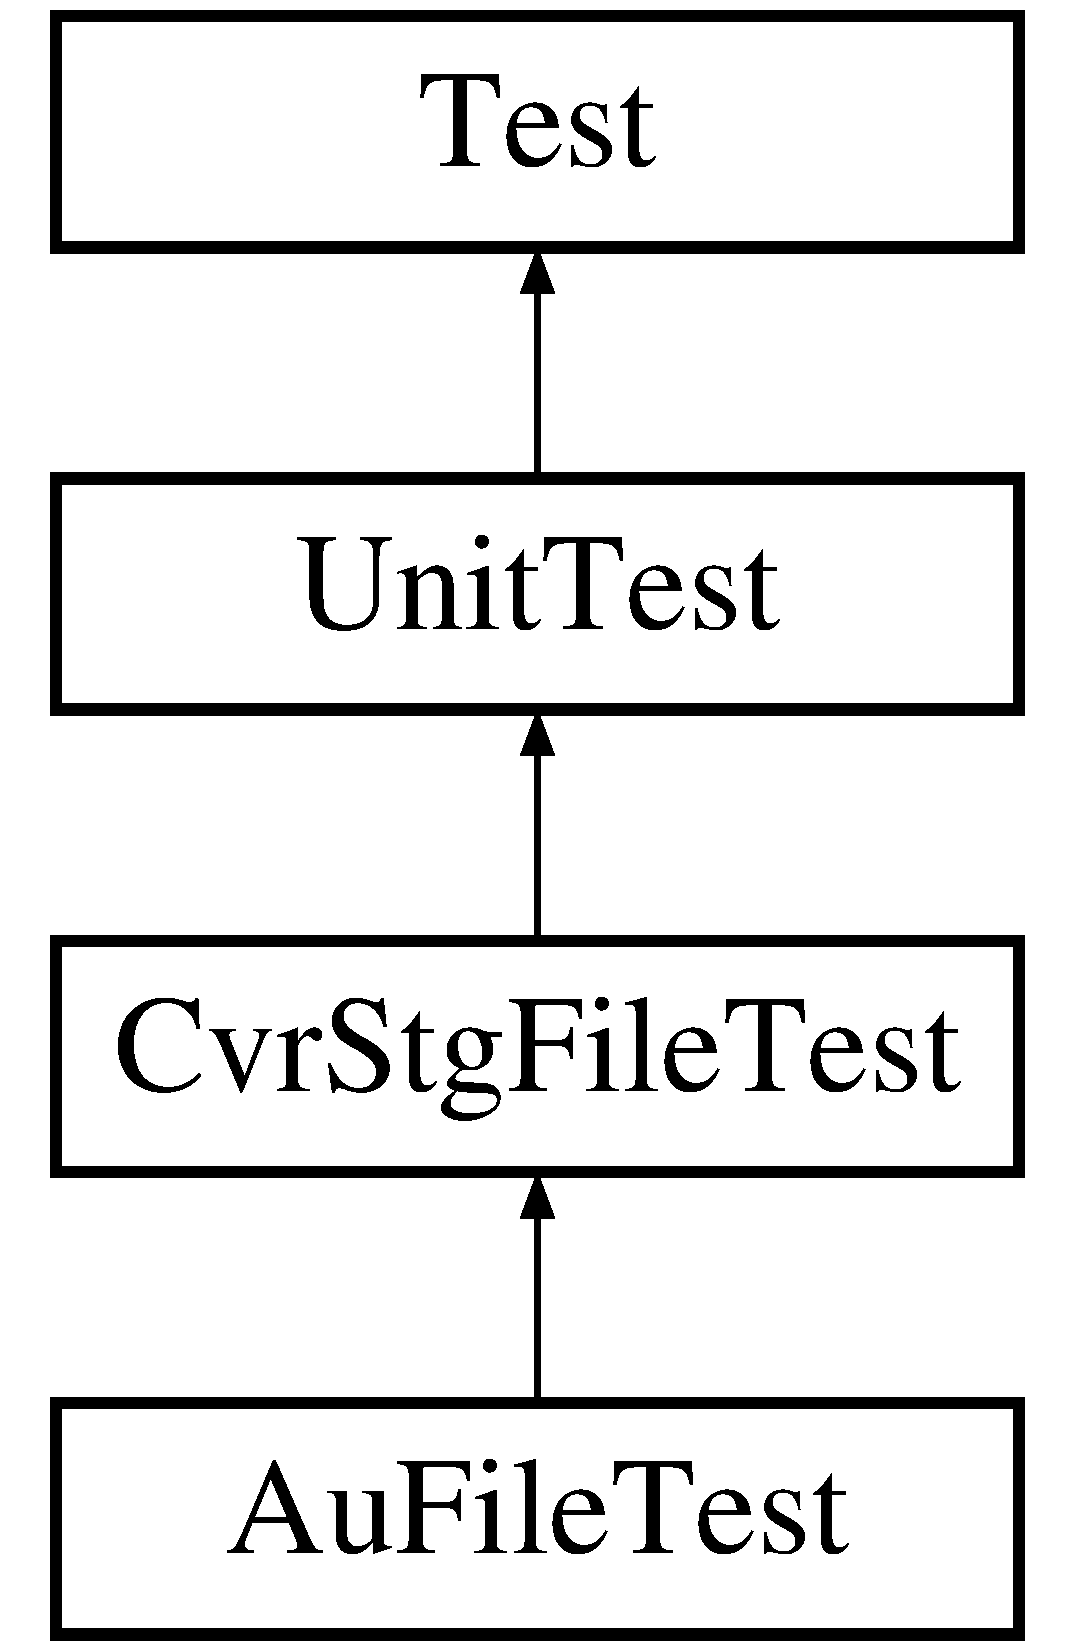
\includegraphics[height=4.000000cm]{classAuFileTest}
\end{center}
\end{figure}
\subsection*{Public Member Functions}
\begin{DoxyCompactItemize}
\item 
\textbf{ Au\+File\+Test} (\textbf{ Test\+Suite} $\ast$s)
\item 
void \textbf{ setup} (void)
\item 
void \textbf{ cleanup} (void)
\item 
void \textbf{ test\+Read\+Write} (void)
\item 
void \textbf{ test\+Read\+Embed\+Extract} (void)
\item 
void \textbf{ test\+Read\+Embed\+Write\+Read\+Extract} (void)
\item 
void \textbf{ test\+Position} (void)
\item 
void \textbf{ test\+Read\+Extract\+Compare} (void)
\item 
void \textbf{ test\+Embedded\+Value} (void)
\end{DoxyCompactItemize}
\subsection*{Private Attributes}
\begin{DoxyCompactItemize}
\item 
\textbf{ Bit\+String} $\ast$ \textbf{ bs1}
\item 
\textbf{ Bit\+String} $\ast$ \textbf{ bs2}
\item 
\textbf{ Bit\+String} $\ast$ \textbf{ bs3}
\item 
\textbf{ Cvr\+Stg\+File} $\ast$ \textbf{ f1}
\item 
\textbf{ Cvr\+Stg\+File} $\ast$ \textbf{ f2}
\item 
\textbf{ Cvr\+Stg\+File} $\ast$ \textbf{ f3}
\item 
\textbf{ Globals} \textbf{ gl1}
\item 
\textbf{ Globals} \textbf{ gl2}
\item 
\textbf{ Globals} \textbf{ gl3}
\end{DoxyCompactItemize}
\subsection*{Additional Inherited Members}


\subsection{Constructor \& Destructor Documentation}
\mbox{\label{classAuFileTest_adf6f137493c0066d906f55293384901a}} 
\index{Au\+File\+Test@{Au\+File\+Test}!Au\+File\+Test@{Au\+File\+Test}}
\index{Au\+File\+Test@{Au\+File\+Test}!Au\+File\+Test@{Au\+File\+Test}}
\subsubsection{Au\+File\+Test()}
{\footnotesize\ttfamily Au\+File\+Test\+::\+Au\+File\+Test (\begin{DoxyParamCaption}\item[{\textbf{ Test\+Suite} $\ast$}]{s }\end{DoxyParamCaption})}



\subsection{Member Function Documentation}
\mbox{\label{classAuFileTest_a10ebf29919259a98f435645885bf856f}} 
\index{Au\+File\+Test@{Au\+File\+Test}!cleanup@{cleanup}}
\index{cleanup@{cleanup}!Au\+File\+Test@{Au\+File\+Test}}
\subsubsection{cleanup()}
{\footnotesize\ttfamily void Au\+File\+Test\+::cleanup (\begin{DoxyParamCaption}\item[{void}]{ }\end{DoxyParamCaption})\hspace{0.3cm}{\ttfamily [virtual]}}

cleanup the unit test -\/ called after run 

Reimplemented from \textbf{ Unit\+Test} \doxyref{}{p.}{classUnitTest_adf77efe972ee4a766d94e3f7ddc193ad}.

\mbox{\label{classAuFileTest_a2f2b853a21a4fd46f1010a1ee474a9a1}} 
\index{Au\+File\+Test@{Au\+File\+Test}!setup@{setup}}
\index{setup@{setup}!Au\+File\+Test@{Au\+File\+Test}}
\subsubsection{setup()}
{\footnotesize\ttfamily void Au\+File\+Test\+::setup (\begin{DoxyParamCaption}\item[{void}]{ }\end{DoxyParamCaption})\hspace{0.3cm}{\ttfamily [virtual]}}

setup the unit test -\/ called before run

\doxyref{Unit\+Test\+::setup}{p.}{classUnitTest_ad73fdf9012b651047ea001d21f9d27ad} will (together with \doxyref{Unit\+Test\+::cleanup}{p.}{classUnitTest_adf77efe972ee4a766d94e3f7ddc193ad}) save and restore the object stored in Globs so they should be called from the corresponding functions in the derived object if the derived unit test manipulates the Globs object. 

Reimplemented from \textbf{ Unit\+Test} \doxyref{}{p.}{classUnitTest_ad73fdf9012b651047ea001d21f9d27ad}.

\mbox{\label{classAuFileTest_a5dd13b6323db882a381b7bf91267bec2}} 
\index{Au\+File\+Test@{Au\+File\+Test}!test\+Embedded\+Value@{test\+Embedded\+Value}}
\index{test\+Embedded\+Value@{test\+Embedded\+Value}!Au\+File\+Test@{Au\+File\+Test}}
\subsubsection{test\+Embedded\+Value()}
{\footnotesize\ttfamily void Au\+File\+Test\+::test\+Embedded\+Value (\begin{DoxyParamCaption}\item[{void}]{ }\end{DoxyParamCaption})}

\mbox{\label{classAuFileTest_a350e286890726565387d78fd33b9c910}} 
\index{Au\+File\+Test@{Au\+File\+Test}!test\+Position@{test\+Position}}
\index{test\+Position@{test\+Position}!Au\+File\+Test@{Au\+File\+Test}}
\subsubsection{test\+Position()}
{\footnotesize\ttfamily void Au\+File\+Test\+::test\+Position (\begin{DoxyParamCaption}\item[{void}]{ }\end{DoxyParamCaption})}

\mbox{\label{classAuFileTest_a0b231ad8f4aa0e0430f195b5c9b1b62d}} 
\index{Au\+File\+Test@{Au\+File\+Test}!test\+Read\+Embed\+Extract@{test\+Read\+Embed\+Extract}}
\index{test\+Read\+Embed\+Extract@{test\+Read\+Embed\+Extract}!Au\+File\+Test@{Au\+File\+Test}}
\subsubsection{test\+Read\+Embed\+Extract()}
{\footnotesize\ttfamily void Au\+File\+Test\+::test\+Read\+Embed\+Extract (\begin{DoxyParamCaption}\item[{void}]{ }\end{DoxyParamCaption})}

\mbox{\label{classAuFileTest_a371d1ef5cc425015738dc0f8d7e6527f}} 
\index{Au\+File\+Test@{Au\+File\+Test}!test\+Read\+Embed\+Write\+Read\+Extract@{test\+Read\+Embed\+Write\+Read\+Extract}}
\index{test\+Read\+Embed\+Write\+Read\+Extract@{test\+Read\+Embed\+Write\+Read\+Extract}!Au\+File\+Test@{Au\+File\+Test}}
\subsubsection{test\+Read\+Embed\+Write\+Read\+Extract()}
{\footnotesize\ttfamily void Au\+File\+Test\+::test\+Read\+Embed\+Write\+Read\+Extract (\begin{DoxyParamCaption}\item[{void}]{ }\end{DoxyParamCaption})}

\mbox{\label{classAuFileTest_ab3b3582b5c25f87141d58960201168e0}} 
\index{Au\+File\+Test@{Au\+File\+Test}!test\+Read\+Extract\+Compare@{test\+Read\+Extract\+Compare}}
\index{test\+Read\+Extract\+Compare@{test\+Read\+Extract\+Compare}!Au\+File\+Test@{Au\+File\+Test}}
\subsubsection{test\+Read\+Extract\+Compare()}
{\footnotesize\ttfamily void Au\+File\+Test\+::test\+Read\+Extract\+Compare (\begin{DoxyParamCaption}\item[{void}]{ }\end{DoxyParamCaption})}

\mbox{\label{classAuFileTest_afb576a199192946f6fb3f0be480af1f4}} 
\index{Au\+File\+Test@{Au\+File\+Test}!test\+Read\+Write@{test\+Read\+Write}}
\index{test\+Read\+Write@{test\+Read\+Write}!Au\+File\+Test@{Au\+File\+Test}}
\subsubsection{test\+Read\+Write()}
{\footnotesize\ttfamily void Au\+File\+Test\+::test\+Read\+Write (\begin{DoxyParamCaption}\item[{void}]{ }\end{DoxyParamCaption})}



\subsection{Member Data Documentation}
\mbox{\label{classAuFileTest_a92fb65918ef53f3d916bd61dafb11d91}} 
\index{Au\+File\+Test@{Au\+File\+Test}!bs1@{bs1}}
\index{bs1@{bs1}!Au\+File\+Test@{Au\+File\+Test}}
\subsubsection{bs1}
{\footnotesize\ttfamily \textbf{ Bit\+String}$\ast$ Au\+File\+Test\+::bs1\hspace{0.3cm}{\ttfamily [private]}}

\mbox{\label{classAuFileTest_abdc7d1c97af31f3a41e91377c9c5826a}} 
\index{Au\+File\+Test@{Au\+File\+Test}!bs2@{bs2}}
\index{bs2@{bs2}!Au\+File\+Test@{Au\+File\+Test}}
\subsubsection{bs2}
{\footnotesize\ttfamily \textbf{ Bit\+String} $\ast$ Au\+File\+Test\+::bs2\hspace{0.3cm}{\ttfamily [private]}}

\mbox{\label{classAuFileTest_adbc8359f064b8a2d38edaccd907bedae}} 
\index{Au\+File\+Test@{Au\+File\+Test}!bs3@{bs3}}
\index{bs3@{bs3}!Au\+File\+Test@{Au\+File\+Test}}
\subsubsection{bs3}
{\footnotesize\ttfamily \textbf{ Bit\+String} $\ast$ Au\+File\+Test\+::bs3\hspace{0.3cm}{\ttfamily [private]}}

\mbox{\label{classAuFileTest_a9f86b05e9f8d2ea9265bbef8ab1ec854}} 
\index{Au\+File\+Test@{Au\+File\+Test}!f1@{f1}}
\index{f1@{f1}!Au\+File\+Test@{Au\+File\+Test}}
\subsubsection{f1}
{\footnotesize\ttfamily \textbf{ Cvr\+Stg\+File}$\ast$ Au\+File\+Test\+::f1\hspace{0.3cm}{\ttfamily [private]}}

\mbox{\label{classAuFileTest_a4f083a6d7bb3433b3b9e6af52aeee618}} 
\index{Au\+File\+Test@{Au\+File\+Test}!f2@{f2}}
\index{f2@{f2}!Au\+File\+Test@{Au\+File\+Test}}
\subsubsection{f2}
{\footnotesize\ttfamily \textbf{ Cvr\+Stg\+File} $\ast$ Au\+File\+Test\+::f2\hspace{0.3cm}{\ttfamily [private]}}

\mbox{\label{classAuFileTest_a2785eda74685e7a2c05047d6f30d4699}} 
\index{Au\+File\+Test@{Au\+File\+Test}!f3@{f3}}
\index{f3@{f3}!Au\+File\+Test@{Au\+File\+Test}}
\subsubsection{f3}
{\footnotesize\ttfamily \textbf{ Cvr\+Stg\+File} $\ast$ Au\+File\+Test\+::f3\hspace{0.3cm}{\ttfamily [private]}}

\mbox{\label{classAuFileTest_a3311376cef3d9a5c38ff0077d4a54490}} 
\index{Au\+File\+Test@{Au\+File\+Test}!gl1@{gl1}}
\index{gl1@{gl1}!Au\+File\+Test@{Au\+File\+Test}}
\subsubsection{gl1}
{\footnotesize\ttfamily \textbf{ Globals} Au\+File\+Test\+::gl1\hspace{0.3cm}{\ttfamily [private]}}

\mbox{\label{classAuFileTest_a329ca7f4d3e2eefefdbcb01bfbe09955}} 
\index{Au\+File\+Test@{Au\+File\+Test}!gl2@{gl2}}
\index{gl2@{gl2}!Au\+File\+Test@{Au\+File\+Test}}
\subsubsection{gl2}
{\footnotesize\ttfamily \textbf{ Globals} Au\+File\+Test\+::gl2\hspace{0.3cm}{\ttfamily [private]}}

\mbox{\label{classAuFileTest_a8dfe96a1013553f1bff762dc6dbed66c}} 
\index{Au\+File\+Test@{Au\+File\+Test}!gl3@{gl3}}
\index{gl3@{gl3}!Au\+File\+Test@{Au\+File\+Test}}
\subsubsection{gl3}
{\footnotesize\ttfamily \textbf{ Globals} Au\+File\+Test\+::gl3\hspace{0.3cm}{\ttfamily [private]}}



The documentation for this class was generated from the following files\+:\begin{DoxyCompactItemize}
\item 
\textbf{ Au\+File\+Test.\+h}\item 
\textbf{ Au\+File\+Test.\+cc}\end{DoxyCompactItemize}

\section{Au\+File\+:\+:Au\+Header Class Reference}
\label{classAuFile_1_1AuHeader}\index{Au\+File\+::\+Au\+Header@{Au\+File\+::\+Au\+Header}}
\subsection*{Public Member Functions}
\begin{DoxyCompactItemize}
\item 
unsigned short \textbf{ get\+Bytes\+Per\+Sample} (void) const
\end{DoxyCompactItemize}
\subsection*{Public Attributes}
\begin{DoxyCompactItemize}
\item 
char \textbf{ id} [4]
\item 
\textbf{ U\+W\+O\+R\+D32} \textbf{ offset}
\item 
\textbf{ U\+W\+O\+R\+D32} \textbf{ size}
\item 
\textbf{ E\+N\+C\+O\+D\+I\+NG} \textbf{ encoding}
\item 
\textbf{ U\+W\+O\+R\+D32} \textbf{ samplerate}
\item 
\textbf{ U\+W\+O\+R\+D32} \textbf{ channels}
\end{DoxyCompactItemize}
\subsection*{Static Public Attributes}
\begin{DoxyCompactItemize}
\item 
static const \textbf{ U\+W\+O\+R\+D32} \textbf{ Size\+Unknown} = 0x\+F\+F\+F\+F\+F\+F\+FF
\item 
static const unsigned short \textbf{ Header\+Size} = 24
\end{DoxyCompactItemize}


\subsection{Member Function Documentation}
\mbox{\label{classAuFile_1_1AuHeader_a2282e7c4a6d8a3b5d3fa61ec9da8c3ce}} 
\index{Au\+File\+::\+Au\+Header@{Au\+File\+::\+Au\+Header}!get\+Bytes\+Per\+Sample@{get\+Bytes\+Per\+Sample}}
\index{get\+Bytes\+Per\+Sample@{get\+Bytes\+Per\+Sample}!Au\+File\+::\+Au\+Header@{Au\+File\+::\+Au\+Header}}
\subsubsection{get\+Bytes\+Per\+Sample()}
{\footnotesize\ttfamily unsigned short Au\+File\+::\+Au\+Header\+::get\+Bytes\+Per\+Sample (\begin{DoxyParamCaption}\item[{void}]{ }\end{DoxyParamCaption}) const}



\subsection{Member Data Documentation}
\mbox{\label{classAuFile_1_1AuHeader_a6b283f9b7d02ef0def4edc67f359d646}} 
\index{Au\+File\+::\+Au\+Header@{Au\+File\+::\+Au\+Header}!channels@{channels}}
\index{channels@{channels}!Au\+File\+::\+Au\+Header@{Au\+File\+::\+Au\+Header}}
\subsubsection{channels}
{\footnotesize\ttfamily \textbf{ U\+W\+O\+R\+D32} Au\+File\+::\+Au\+Header\+::channels}

\mbox{\label{classAuFile_1_1AuHeader_a463aaa38af82f54346c97f853e4e7240}} 
\index{Au\+File\+::\+Au\+Header@{Au\+File\+::\+Au\+Header}!encoding@{encoding}}
\index{encoding@{encoding}!Au\+File\+::\+Au\+Header@{Au\+File\+::\+Au\+Header}}
\subsubsection{encoding}
{\footnotesize\ttfamily \textbf{ E\+N\+C\+O\+D\+I\+NG} Au\+File\+::\+Au\+Header\+::encoding}

\mbox{\label{classAuFile_1_1AuHeader_aaf8f81ce6c30d831ec20706cbc3a075c}} 
\index{Au\+File\+::\+Au\+Header@{Au\+File\+::\+Au\+Header}!Header\+Size@{Header\+Size}}
\index{Header\+Size@{Header\+Size}!Au\+File\+::\+Au\+Header@{Au\+File\+::\+Au\+Header}}
\subsubsection{Header\+Size}
{\footnotesize\ttfamily const unsigned short Au\+File\+::\+Au\+Header\+::\+Header\+Size = 24\hspace{0.3cm}{\ttfamily [static]}}

\mbox{\label{classAuFile_1_1AuHeader_a64c598b07cf8a332717f8164439d4590}} 
\index{Au\+File\+::\+Au\+Header@{Au\+File\+::\+Au\+Header}!id@{id}}
\index{id@{id}!Au\+File\+::\+Au\+Header@{Au\+File\+::\+Au\+Header}}
\subsubsection{id}
{\footnotesize\ttfamily char Au\+File\+::\+Au\+Header\+::id[4]}

\mbox{\label{classAuFile_1_1AuHeader_a10a77d6fb987e8b81957b6ff8cf39e48}} 
\index{Au\+File\+::\+Au\+Header@{Au\+File\+::\+Au\+Header}!offset@{offset}}
\index{offset@{offset}!Au\+File\+::\+Au\+Header@{Au\+File\+::\+Au\+Header}}
\subsubsection{offset}
{\footnotesize\ttfamily \textbf{ U\+W\+O\+R\+D32} Au\+File\+::\+Au\+Header\+::offset}

\mbox{\label{classAuFile_1_1AuHeader_a92115913881cd43e7c1f0a0fa4c97a68}} 
\index{Au\+File\+::\+Au\+Header@{Au\+File\+::\+Au\+Header}!samplerate@{samplerate}}
\index{samplerate@{samplerate}!Au\+File\+::\+Au\+Header@{Au\+File\+::\+Au\+Header}}
\subsubsection{samplerate}
{\footnotesize\ttfamily \textbf{ U\+W\+O\+R\+D32} Au\+File\+::\+Au\+Header\+::samplerate}

\mbox{\label{classAuFile_1_1AuHeader_ad01f795eaf3f88c0fdcaf7ef7e28576e}} 
\index{Au\+File\+::\+Au\+Header@{Au\+File\+::\+Au\+Header}!size@{size}}
\index{size@{size}!Au\+File\+::\+Au\+Header@{Au\+File\+::\+Au\+Header}}
\subsubsection{size}
{\footnotesize\ttfamily \textbf{ U\+W\+O\+R\+D32} Au\+File\+::\+Au\+Header\+::size}

\mbox{\label{classAuFile_1_1AuHeader_a8b59a6efac10f758e8ba6f8dbe8f94f2}} 
\index{Au\+File\+::\+Au\+Header@{Au\+File\+::\+Au\+Header}!Size\+Unknown@{Size\+Unknown}}
\index{Size\+Unknown@{Size\+Unknown}!Au\+File\+::\+Au\+Header@{Au\+File\+::\+Au\+Header}}
\subsubsection{Size\+Unknown}
{\footnotesize\ttfamily const \textbf{ U\+W\+O\+R\+D32} Au\+File\+::\+Au\+Header\+::\+Size\+Unknown = 0x\+F\+F\+F\+F\+F\+F\+FF\hspace{0.3cm}{\ttfamily [static]}}



The documentation for this class was generated from the following files\+:\begin{DoxyCompactItemize}
\item 
\textbf{ Au\+File.\+h}\item 
\textbf{ Au\+File.\+cc}\end{DoxyCompactItemize}

\section{A\+Utils Class Reference}
\label{classAUtils}\index{A\+Utils@{A\+Utils}}


provides some generic functions for non-\/standard arithmetic operations  




{\ttfamily \#include $<$A\+Utils.\+h$>$}

\subsection*{Static Public Member Functions}
\begin{DoxyCompactItemize}
\item 
{\footnotesize template$<$class T $>$ }\\static T \textbf{ max} (T a, T b)
\item 
{\footnotesize template$<$class T $>$ }\\static T \textbf{ min} (T a, T b)
\item 
{\footnotesize template$<$class T $>$ }\\static T \textbf{ div\+\_\+roundup} (T a, T b)
\item 
{\footnotesize template$<$class T $>$ }\\static T \textbf{ bminus} (T a, T b)
\item 
{\footnotesize template$<$class T , T top$>$ }\\static T \textbf{ bplus} (T a, T b)
\item 
{\footnotesize template$<$class T $>$ }\\static T \textbf{ bplus} (T a, T b, T top)
\item 
{\footnotesize template$<$class T , class C\+T\+Y\+PE $>$ }\\static T \textbf{ modsum} (T $\ast$s, C\+T\+Y\+PE n, T m)
\item 
{\footnotesize template$<$class IT , class FT $>$ }\\static IT \textbf{ roundup} (FT x)
\item 
{\footnotesize template$<$class T $>$ }\\static T \textbf{ log2\+\_\+ceil} (T n)
\end{DoxyCompactItemize}


\subsection{Member Function Documentation}
\mbox{\label{classAUtils_a913619524397350adb0e1c047b378a58}} 
\index{A\+Utils@{A\+Utils}!bminus@{bminus}}
\index{bminus@{bminus}!A\+Utils@{A\+Utils}}
\subsubsection{bminus()}
{\footnotesize\ttfamily template$<$class T $>$ \\
T A\+Utils\+::bminus (\begin{DoxyParamCaption}\item[{T}]{a,  }\item[{T}]{b }\end{DoxyParamCaption})\hspace{0.3cm}{\ttfamily [static]}}

substraction with the modification to return 0 (T()) for negative difference (needs $>$, -\/, T()) \mbox{\label{classAUtils_a2195cee438b25dd9794334914ee31588}} 
\index{A\+Utils@{A\+Utils}!bplus@{bplus}}
\index{bplus@{bplus}!A\+Utils@{A\+Utils}}
\subsubsection{bplus()\hspace{0.1cm}{\footnotesize\ttfamily [1/2]}}
{\footnotesize\ttfamily template$<$class T , T top$>$ \\
T A\+Utils\+::bplus (\begin{DoxyParamCaption}\item[{T}]{a,  }\item[{T}]{b }\end{DoxyParamCaption})\hspace{0.3cm}{\ttfamily [static]}}

addition with the modification to return top for sums that are larger than top \mbox{\label{classAUtils_a0150b72b95e38e28588ffcae0d10e0a0}} 
\index{A\+Utils@{A\+Utils}!bplus@{bplus}}
\index{bplus@{bplus}!A\+Utils@{A\+Utils}}
\subsubsection{bplus()\hspace{0.1cm}{\footnotesize\ttfamily [2/2]}}
{\footnotesize\ttfamily template$<$class T $>$ \\
T A\+Utils\+::bplus (\begin{DoxyParamCaption}\item[{T}]{a,  }\item[{T}]{b,  }\item[{T}]{top }\end{DoxyParamCaption})\hspace{0.3cm}{\ttfamily [static]}}

\mbox{\label{classAUtils_a447da3912ebadf1c8e387c41b8564d21}} 
\index{A\+Utils@{A\+Utils}!div\+\_\+roundup@{div\+\_\+roundup}}
\index{div\+\_\+roundup@{div\+\_\+roundup}!A\+Utils@{A\+Utils}}
\subsubsection{div\+\_\+roundup()}
{\footnotesize\ttfamily template$<$class T $>$ \\
T A\+Utils\+::div\+\_\+roundup (\begin{DoxyParamCaption}\item[{T}]{a,  }\item[{T}]{b }\end{DoxyParamCaption})\hspace{0.3cm}{\ttfamily [static]}}

returns a divided through b rounded up to nearest \char`\"{}integer\char`\"{} (needs =, --, +, /) \mbox{\label{classAUtils_a139c8f7686c2d57cbac08bb875612eee}} 
\index{A\+Utils@{A\+Utils}!log2\+\_\+ceil@{log2\+\_\+ceil}}
\index{log2\+\_\+ceil@{log2\+\_\+ceil}!A\+Utils@{A\+Utils}}
\subsubsection{log2\+\_\+ceil()}
{\footnotesize\ttfamily template$<$class T $>$ \\
T A\+Utils\+::log2\+\_\+ceil (\begin{DoxyParamCaption}\item[{T}]{n }\end{DoxyParamCaption})\hspace{0.3cm}{\ttfamily [static]}}

compute 2-\/logarithm of n (rounded up to nearest int), i.\+e. number of bits needed to store values from \{0,...,n-\/1\} \mbox{\label{classAUtils_a78af5cdca7b9ad8f5bda06e1a16f62be}} 
\index{A\+Utils@{A\+Utils}!max@{max}}
\index{max@{max}!A\+Utils@{A\+Utils}}
\subsubsection{max()}
{\footnotesize\ttfamily template$<$class T $>$ \\
T A\+Utils\+::max (\begin{DoxyParamCaption}\item[{T}]{a,  }\item[{T}]{b }\end{DoxyParamCaption})\hspace{0.3cm}{\ttfamily [static]}}

return the maximum of a and b (needs $>$) \mbox{\label{classAUtils_a526333c7b780b8b99e62dc7d87caa50b}} 
\index{A\+Utils@{A\+Utils}!min@{min}}
\index{min@{min}!A\+Utils@{A\+Utils}}
\subsubsection{min()}
{\footnotesize\ttfamily template$<$class T $>$ \\
T A\+Utils\+::min (\begin{DoxyParamCaption}\item[{T}]{a,  }\item[{T}]{b }\end{DoxyParamCaption})\hspace{0.3cm}{\ttfamily [static]}}

return the minimum of a and b (needs $<$) \mbox{\label{classAUtils_a60bf7adcf99889a97a02bcb4c5290080}} 
\index{A\+Utils@{A\+Utils}!modsum@{modsum}}
\index{modsum@{modsum}!A\+Utils@{A\+Utils}}
\subsubsection{modsum()}
{\footnotesize\ttfamily template$<$class T , class C\+T\+Y\+PE $>$ \\
T A\+Utils\+::modsum (\begin{DoxyParamCaption}\item[{T $\ast$}]{s,  }\item[{C\+T\+Y\+PE}]{n,  }\item[{T}]{m }\end{DoxyParamCaption})\hspace{0.3cm}{\ttfamily [static]}}

calculate the sum s[0]+...s[n-\/1] modulo m (needs =, +, \% for T and =, C\+T\+Y\+P\+E(), $<$, ++ for C\+T\+Y\+PE) \mbox{\label{classAUtils_a978c57821e2acd0f8560aa3b1d866c07}} 
\index{A\+Utils@{A\+Utils}!roundup@{roundup}}
\index{roundup@{roundup}!A\+Utils@{A\+Utils}}
\subsubsection{roundup()}
{\footnotesize\ttfamily template$<$class IT , class FT $>$ \\
IT A\+Utils\+::roundup (\begin{DoxyParamCaption}\item[{FT}]{x }\end{DoxyParamCaption})\hspace{0.3cm}{\ttfamily [static]}}

round up x to nearest integer 

The documentation for this class was generated from the following file\+:\begin{DoxyCompactItemize}
\item 
\textbf{ A\+Utils.\+h}\end{DoxyCompactItemize}

\section{A\+Utils\+Test Class Reference}
\label{classAUtilsTest}\index{A\+Utils\+Test@{A\+Utils\+Test}}


{\ttfamily \#include $<$A\+Utils\+Test.\+h$>$}

Inheritance diagram for A\+Utils\+Test\+:\begin{figure}[H]
\begin{center}
\leavevmode
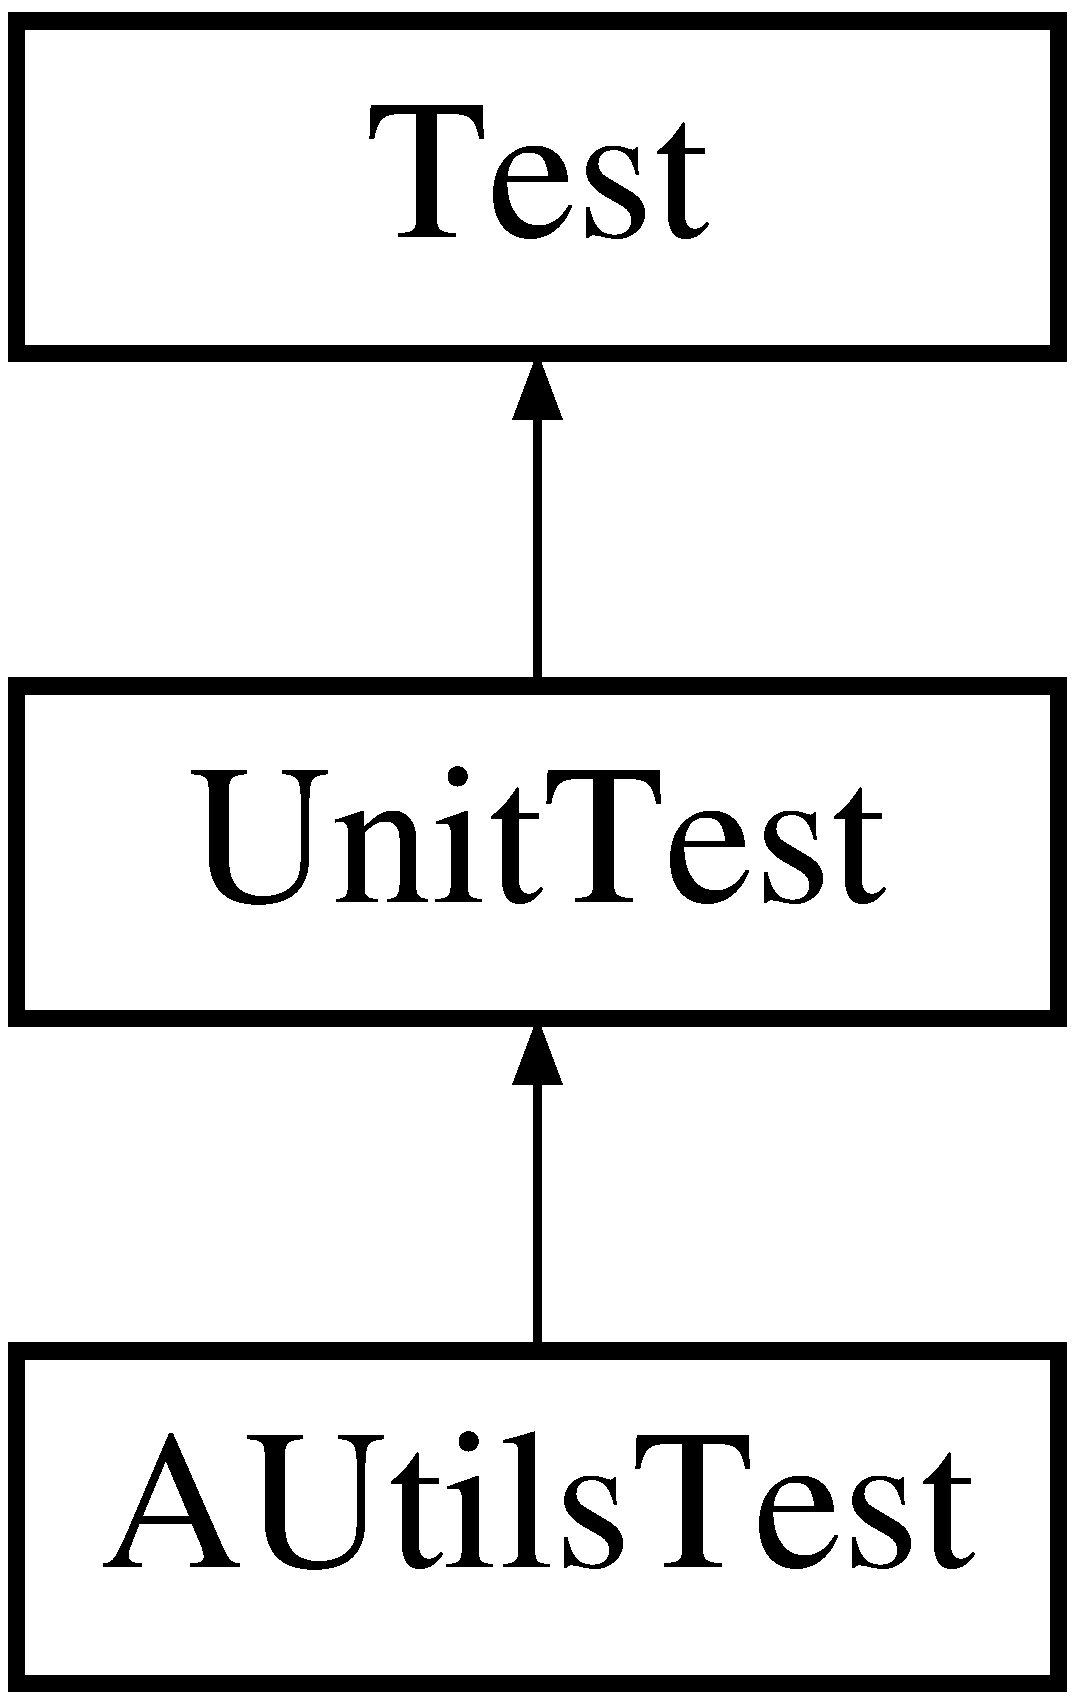
\includegraphics[height=3.000000cm]{classAUtilsTest}
\end{center}
\end{figure}
\subsection*{Public Member Functions}
\begin{DoxyCompactItemize}
\item 
\textbf{ A\+Utils\+Test} (\textbf{ Test\+Suite} $\ast$s)
\item 
void \textbf{ test\+Log2} (void)
\end{DoxyCompactItemize}
\subsection*{Private Member Functions}
\begin{DoxyCompactItemize}
\item 
bool \textbf{ generic\+Test\+Log2} (int n, double res)
\end{DoxyCompactItemize}
\subsection*{Additional Inherited Members}


\subsection{Constructor \& Destructor Documentation}
\mbox{\label{classAUtilsTest_a58f82e2d0191d41e671a26030ab033d3}} 
\index{A\+Utils\+Test@{A\+Utils\+Test}!A\+Utils\+Test@{A\+Utils\+Test}}
\index{A\+Utils\+Test@{A\+Utils\+Test}!A\+Utils\+Test@{A\+Utils\+Test}}
\subsubsection{A\+Utils\+Test()}
{\footnotesize\ttfamily A\+Utils\+Test\+::\+A\+Utils\+Test (\begin{DoxyParamCaption}\item[{\textbf{ Test\+Suite} $\ast$}]{s }\end{DoxyParamCaption})}



\subsection{Member Function Documentation}
\mbox{\label{classAUtilsTest_a30344faee4e3828463097724939777e9}} 
\index{A\+Utils\+Test@{A\+Utils\+Test}!generic\+Test\+Log2@{generic\+Test\+Log2}}
\index{generic\+Test\+Log2@{generic\+Test\+Log2}!A\+Utils\+Test@{A\+Utils\+Test}}
\subsubsection{generic\+Test\+Log2()}
{\footnotesize\ttfamily bool A\+Utils\+Test\+::generic\+Test\+Log2 (\begin{DoxyParamCaption}\item[{int}]{n,  }\item[{double}]{res }\end{DoxyParamCaption})\hspace{0.3cm}{\ttfamily [private]}}

\mbox{\label{classAUtilsTest_a7dc7f87eedb991a44bccbd29b7ccec38}} 
\index{A\+Utils\+Test@{A\+Utils\+Test}!test\+Log2@{test\+Log2}}
\index{test\+Log2@{test\+Log2}!A\+Utils\+Test@{A\+Utils\+Test}}
\subsubsection{test\+Log2()}
{\footnotesize\ttfamily void A\+Utils\+Test\+::test\+Log2 (\begin{DoxyParamCaption}\item[{void}]{ }\end{DoxyParamCaption})}



The documentation for this class was generated from the following files\+:\begin{DoxyCompactItemize}
\item 
\textbf{ A\+Utils\+Test.\+h}\item 
\textbf{ A\+Utils\+Test.\+cc}\end{DoxyCompactItemize}

\section{B\+F\+S\+A\+P\+Heuristic Class Reference}
\label{classBFSAPHeuristic}\index{B\+F\+S\+A\+P\+Heuristic@{B\+F\+S\+A\+P\+Heuristic}}


a matching algorithm implementing a heuristic breadth-\/first-\/search for augmenting paths  




{\ttfamily \#include $<$B\+F\+S\+A\+P\+Heuristic.\+h$>$}

Inheritance diagram for B\+F\+S\+A\+P\+Heuristic\+:\begin{figure}[H]
\begin{center}
\leavevmode
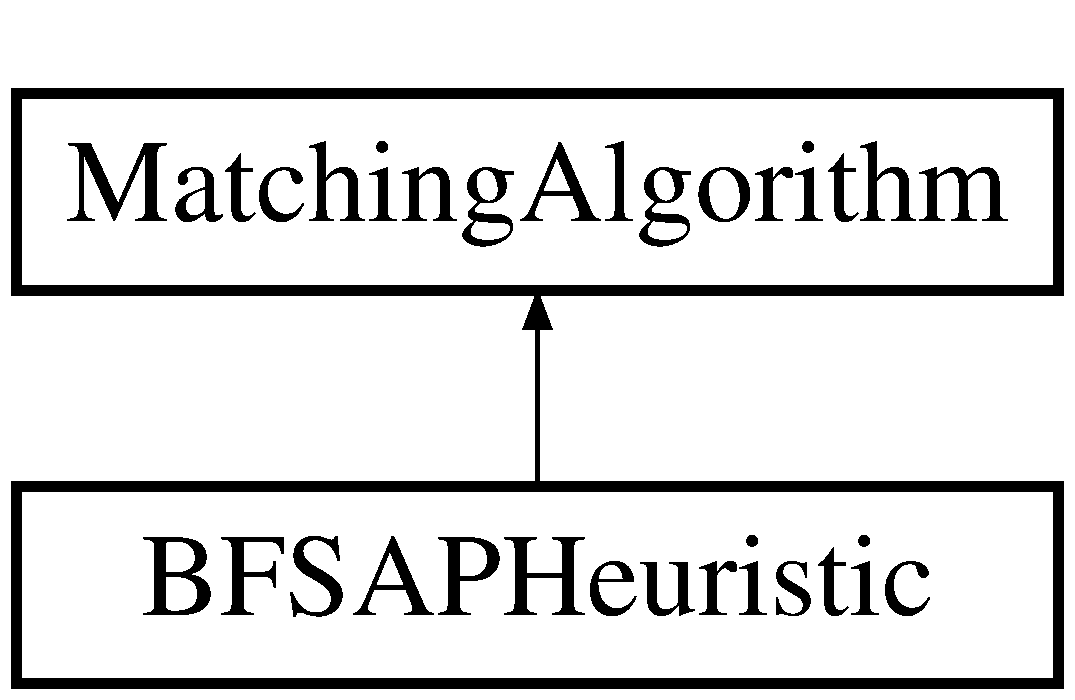
\includegraphics[height=2.000000cm]{classBFSAPHeuristic}
\end{center}
\end{figure}
\subsection*{Public Member Functions}
\begin{DoxyCompactItemize}
\item 
\textbf{ B\+F\+S\+A\+P\+Heuristic} (\textbf{ Graph} $\ast$g, \textbf{ Matching} $\ast$m)
\item 
virtual \textbf{ $\sim$\+B\+F\+S\+A\+P\+Heuristic} (void)
\item 
const char $\ast$ \textbf{ get\+Name} (void) const
\item 
void \textbf{ run} (void)
\end{DoxyCompactItemize}
\subsection*{Private Member Functions}
\begin{DoxyCompactItemize}
\item 
unsigned long \textbf{ search\+Augmenting\+Path} (\textbf{ Vertex} $\ast$v0, const \textbf{ Edge} $\ast$$\ast$path)
\end{DoxyCompactItemize}
\subsection*{Private Attributes}
\begin{DoxyCompactItemize}
\item 
bool $\ast$ \textbf{ Vertex\+Visited}
\item 
\textbf{ Edge} $\ast$ \textbf{ Back\+Edge}
\end{DoxyCompactItemize}
\subsection*{Additional Inherited Members}


\subsection{Constructor \& Destructor Documentation}
\mbox{\label{classBFSAPHeuristic_ad01695f4b13c50e8fefd15fb6813b491}} 
\index{B\+F\+S\+A\+P\+Heuristic@{B\+F\+S\+A\+P\+Heuristic}!B\+F\+S\+A\+P\+Heuristic@{B\+F\+S\+A\+P\+Heuristic}}
\index{B\+F\+S\+A\+P\+Heuristic@{B\+F\+S\+A\+P\+Heuristic}!B\+F\+S\+A\+P\+Heuristic@{B\+F\+S\+A\+P\+Heuristic}}
\subsubsection{B\+F\+S\+A\+P\+Heuristic()}
{\footnotesize\ttfamily B\+F\+S\+A\+P\+Heuristic\+::\+B\+F\+S\+A\+P\+Heuristic (\begin{DoxyParamCaption}\item[{\textbf{ Graph} $\ast$}]{g,  }\item[{\textbf{ Matching} $\ast$}]{m }\end{DoxyParamCaption})}

construct an \doxyref{B\+F\+S\+A\+P\+Heuristic}{p.}{classBFSAPHeuristic} object 
\begin{DoxyParams}{Parameters}
{\em g} & the graph on which this heuristic should run \\
\hline
{\em m} & the matching to start with \\
\hline
\end{DoxyParams}
\mbox{\label{classBFSAPHeuristic_ac5fe4a33565132234933b709becd5644}} 
\index{B\+F\+S\+A\+P\+Heuristic@{B\+F\+S\+A\+P\+Heuristic}!````~B\+F\+S\+A\+P\+Heuristic@{$\sim$\+B\+F\+S\+A\+P\+Heuristic}}
\index{````~B\+F\+S\+A\+P\+Heuristic@{$\sim$\+B\+F\+S\+A\+P\+Heuristic}!B\+F\+S\+A\+P\+Heuristic@{B\+F\+S\+A\+P\+Heuristic}}
\subsubsection{$\sim$\+B\+F\+S\+A\+P\+Heuristic()}
{\footnotesize\ttfamily B\+F\+S\+A\+P\+Heuristic\+::$\sim$\+B\+F\+S\+A\+P\+Heuristic (\begin{DoxyParamCaption}\item[{void}]{ }\end{DoxyParamCaption})\hspace{0.3cm}{\ttfamily [virtual]}}



\subsection{Member Function Documentation}
\mbox{\label{classBFSAPHeuristic_afbd3a55843232ba22bea3360e6009a97}} 
\index{B\+F\+S\+A\+P\+Heuristic@{B\+F\+S\+A\+P\+Heuristic}!get\+Name@{get\+Name}}
\index{get\+Name@{get\+Name}!B\+F\+S\+A\+P\+Heuristic@{B\+F\+S\+A\+P\+Heuristic}}
\subsubsection{get\+Name()}
{\footnotesize\ttfamily const char$\ast$ B\+F\+S\+A\+P\+Heuristic\+::get\+Name (\begin{DoxyParamCaption}\item[{void}]{ }\end{DoxyParamCaption}) const\hspace{0.3cm}{\ttfamily [inline]}, {\ttfamily [virtual]}}



Implements \textbf{ Matching\+Algorithm} \doxyref{}{p.}{classMatchingAlgorithm_a7305edae5d74e91987bcf983b2a1171a}.

\mbox{\label{classBFSAPHeuristic_a2b12948841049cfca3e6d634d793c510}} 
\index{B\+F\+S\+A\+P\+Heuristic@{B\+F\+S\+A\+P\+Heuristic}!run@{run}}
\index{run@{run}!B\+F\+S\+A\+P\+Heuristic@{B\+F\+S\+A\+P\+Heuristic}}
\subsubsection{run()}
{\footnotesize\ttfamily void B\+F\+S\+A\+P\+Heuristic\+::run (\begin{DoxyParamCaption}\item[{void}]{ }\end{DoxyParamCaption})\hspace{0.3cm}{\ttfamily [virtual]}}



Implements \textbf{ Matching\+Algorithm} \doxyref{}{p.}{classMatchingAlgorithm_aeea6c808daf03fd788c9a9feea885c41}.

\mbox{\label{classBFSAPHeuristic_ae03e433e445781a1041ce5ff350e62b9}} 
\index{B\+F\+S\+A\+P\+Heuristic@{B\+F\+S\+A\+P\+Heuristic}!search\+Augmenting\+Path@{search\+Augmenting\+Path}}
\index{search\+Augmenting\+Path@{search\+Augmenting\+Path}!B\+F\+S\+A\+P\+Heuristic@{B\+F\+S\+A\+P\+Heuristic}}
\subsubsection{search\+Augmenting\+Path()}
{\footnotesize\ttfamily unsigned long B\+F\+S\+A\+P\+Heuristic\+::search\+Augmenting\+Path (\begin{DoxyParamCaption}\item[{\textbf{ Vertex} $\ast$}]{v0,  }\item[{const \textbf{ Edge} $\ast$$\ast$}]{path }\end{DoxyParamCaption})\hspace{0.3cm}{\ttfamily [private]}}


\begin{DoxyParams}{Parameters}
{\em v0} & an exposed vertex \\
\hline
{\em path} & an array of \doxyref{Edge}{p.}{classEdge} pointers where the path will be put \\
\hline
\end{DoxyParams}
\begin{DoxyReturn}{Returns}
the length of the path (the number of valid edges in path) 
\end{DoxyReturn}


\subsection{Member Data Documentation}
\mbox{\label{classBFSAPHeuristic_a352e950c3dde1e0c1046adbec7715ca9}} 
\index{B\+F\+S\+A\+P\+Heuristic@{B\+F\+S\+A\+P\+Heuristic}!Back\+Edge@{Back\+Edge}}
\index{Back\+Edge@{Back\+Edge}!B\+F\+S\+A\+P\+Heuristic@{B\+F\+S\+A\+P\+Heuristic}}
\subsubsection{Back\+Edge}
{\footnotesize\ttfamily \textbf{ Edge}$\ast$ B\+F\+S\+A\+P\+Heuristic\+::\+Back\+Edge\hspace{0.3cm}{\ttfamily [private]}}

\mbox{\label{classBFSAPHeuristic_aa7f91fc4148cfd04daa75b517d42805f}} 
\index{B\+F\+S\+A\+P\+Heuristic@{B\+F\+S\+A\+P\+Heuristic}!Vertex\+Visited@{Vertex\+Visited}}
\index{Vertex\+Visited@{Vertex\+Visited}!B\+F\+S\+A\+P\+Heuristic@{B\+F\+S\+A\+P\+Heuristic}}
\subsubsection{Vertex\+Visited}
{\footnotesize\ttfamily bool$\ast$ B\+F\+S\+A\+P\+Heuristic\+::\+Vertex\+Visited\hspace{0.3cm}{\ttfamily [private]}}



The documentation for this class was generated from the following files\+:\begin{DoxyCompactItemize}
\item 
\textbf{ B\+F\+S\+A\+P\+Heuristic.\+h}\item 
\textbf{ B\+F\+S\+A\+P\+Heuristic.\+cc}\end{DoxyCompactItemize}

\section{B\+F\+S\+A\+P\+Heuristic\+Test Class Reference}
\label{classBFSAPHeuristicTest}\index{B\+F\+S\+A\+P\+Heuristic\+Test@{B\+F\+S\+A\+P\+Heuristic\+Test}}


{\ttfamily \#include $<$B\+F\+S\+A\+P\+Heuristic\+Test.\+h$>$}

Inheritance diagram for B\+F\+S\+A\+P\+Heuristic\+Test\+:\begin{figure}[H]
\begin{center}
\leavevmode
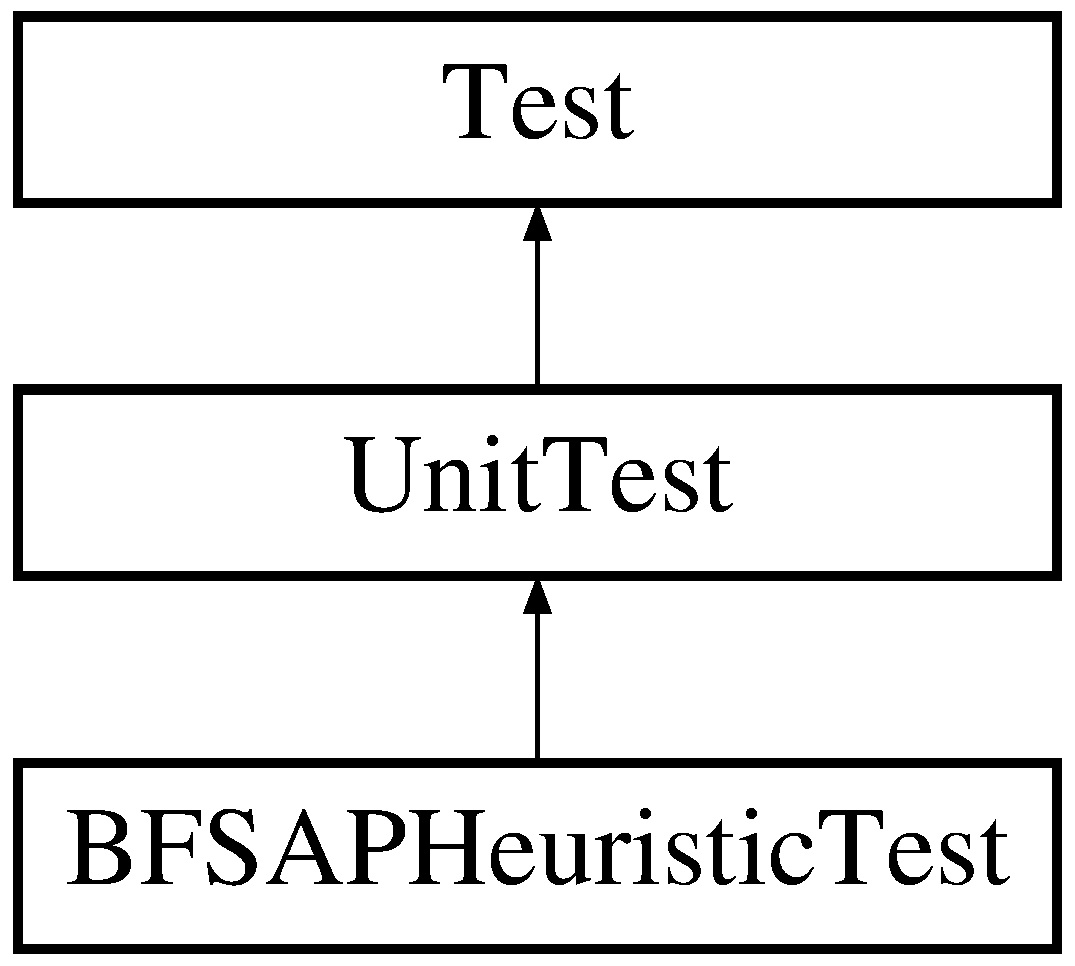
\includegraphics[height=3.000000cm]{classBFSAPHeuristicTest}
\end{center}
\end{figure}
\subsection*{Public Member Functions}
\begin{DoxyCompactItemize}
\item 
\textbf{ B\+F\+S\+A\+P\+Heuristic\+Test} (\textbf{ Test\+Suite} $\ast$s)
\item 
void \textbf{ setup} (void)
\item 
void \textbf{ cleanup} (void)
\item 
void \textbf{ test\+Algorithm} (void)
\end{DoxyCompactItemize}
\subsection*{Private Attributes}
\begin{DoxyCompactItemize}
\item 
\textbf{ Bit\+String} $\ast$ \textbf{ bs1}
\item 
\textbf{ Bit\+String} $\ast$ \textbf{ bs2}
\item 
\textbf{ Bit\+String} $\ast$ \textbf{ bs3}
\item 
\textbf{ Bit\+String} $\ast$ \textbf{ bs4}
\item 
\textbf{ Bit\+String} $\ast$ \textbf{ bs5}
\item 
\textbf{ Cvr\+Stg\+File} $\ast$ \textbf{ f1}
\item 
\textbf{ Cvr\+Stg\+File} $\ast$ \textbf{ f2}
\item 
\textbf{ Cvr\+Stg\+File} $\ast$ \textbf{ f3}
\item 
\textbf{ Cvr\+Stg\+File} $\ast$ \textbf{ f4}
\item 
\textbf{ Cvr\+Stg\+File} $\ast$ \textbf{ f5}
\item 
\textbf{ Selector} $\ast$ \textbf{ s1}
\item 
\textbf{ Selector} $\ast$ \textbf{ s2}
\item 
\textbf{ Selector} $\ast$ \textbf{ s3}
\item 
\textbf{ Selector} $\ast$ \textbf{ s4}
\item 
\textbf{ Selector} $\ast$ \textbf{ s5}
\item 
\textbf{ Graph} $\ast$ \textbf{ g1}
\item 
\textbf{ Graph} $\ast$ \textbf{ g2}
\item 
\textbf{ Graph} $\ast$ \textbf{ g3}
\item 
\textbf{ Graph} $\ast$ \textbf{ g4}
\item 
\textbf{ Graph} $\ast$ \textbf{ g5}
\item 
\textbf{ Matching} $\ast$ \textbf{ m1}
\item 
\textbf{ Matching} $\ast$ \textbf{ m2}
\item 
\textbf{ Matching} $\ast$ \textbf{ m3}
\item 
\textbf{ Matching} $\ast$ \textbf{ m4}
\item 
\textbf{ Matching} $\ast$ \textbf{ m5}
\item 
\textbf{ B\+F\+S\+A\+P\+Heuristic} $\ast$ \textbf{ aph1}
\item 
\textbf{ B\+F\+S\+A\+P\+Heuristic} $\ast$ \textbf{ aph2}
\item 
\textbf{ B\+F\+S\+A\+P\+Heuristic} $\ast$ \textbf{ aph3}
\item 
\textbf{ B\+F\+S\+A\+P\+Heuristic} $\ast$ \textbf{ aph4}
\item 
\textbf{ B\+F\+S\+A\+P\+Heuristic} $\ast$ \textbf{ aph5}
\item 
\textbf{ Globals} \textbf{ gl1}
\item 
\textbf{ Globals} \textbf{ gl2}
\item 
\textbf{ Globals} \textbf{ gl3}
\item 
\textbf{ Globals} \textbf{ gl4}
\item 
\textbf{ Globals} \textbf{ gl5}
\end{DoxyCompactItemize}
\subsection*{Additional Inherited Members}


\subsection{Constructor \& Destructor Documentation}
\mbox{\label{classBFSAPHeuristicTest_ac8026b401917bb6e11c84ca644af4ede}} 
\index{B\+F\+S\+A\+P\+Heuristic\+Test@{B\+F\+S\+A\+P\+Heuristic\+Test}!B\+F\+S\+A\+P\+Heuristic\+Test@{B\+F\+S\+A\+P\+Heuristic\+Test}}
\index{B\+F\+S\+A\+P\+Heuristic\+Test@{B\+F\+S\+A\+P\+Heuristic\+Test}!B\+F\+S\+A\+P\+Heuristic\+Test@{B\+F\+S\+A\+P\+Heuristic\+Test}}
\subsubsection{B\+F\+S\+A\+P\+Heuristic\+Test()}
{\footnotesize\ttfamily B\+F\+S\+A\+P\+Heuristic\+Test\+::\+B\+F\+S\+A\+P\+Heuristic\+Test (\begin{DoxyParamCaption}\item[{\textbf{ Test\+Suite} $\ast$}]{s }\end{DoxyParamCaption})}



\subsection{Member Function Documentation}
\mbox{\label{classBFSAPHeuristicTest_a7ff74226439c2833485f4d388e5d4cd7}} 
\index{B\+F\+S\+A\+P\+Heuristic\+Test@{B\+F\+S\+A\+P\+Heuristic\+Test}!cleanup@{cleanup}}
\index{cleanup@{cleanup}!B\+F\+S\+A\+P\+Heuristic\+Test@{B\+F\+S\+A\+P\+Heuristic\+Test}}
\subsubsection{cleanup()}
{\footnotesize\ttfamily void B\+F\+S\+A\+P\+Heuristic\+Test\+::cleanup (\begin{DoxyParamCaption}\item[{void}]{ }\end{DoxyParamCaption})\hspace{0.3cm}{\ttfamily [virtual]}}

cleanup the unit test -\/ called after run 

Reimplemented from \textbf{ Unit\+Test} \doxyref{}{p.}{classUnitTest_adf77efe972ee4a766d94e3f7ddc193ad}.

\mbox{\label{classBFSAPHeuristicTest_ac0e8dd9221ca2f22b27d19cb6b7881f7}} 
\index{B\+F\+S\+A\+P\+Heuristic\+Test@{B\+F\+S\+A\+P\+Heuristic\+Test}!setup@{setup}}
\index{setup@{setup}!B\+F\+S\+A\+P\+Heuristic\+Test@{B\+F\+S\+A\+P\+Heuristic\+Test}}
\subsubsection{setup()}
{\footnotesize\ttfamily void B\+F\+S\+A\+P\+Heuristic\+Test\+::setup (\begin{DoxyParamCaption}\item[{void}]{ }\end{DoxyParamCaption})\hspace{0.3cm}{\ttfamily [virtual]}}

setup the unit test -\/ called before run

\doxyref{Unit\+Test\+::setup}{p.}{classUnitTest_ad73fdf9012b651047ea001d21f9d27ad} will (together with \doxyref{Unit\+Test\+::cleanup}{p.}{classUnitTest_adf77efe972ee4a766d94e3f7ddc193ad}) save and restore the object stored in Globs so they should be called from the corresponding functions in the derived object if the derived unit test manipulates the Globs object. 

Reimplemented from \textbf{ Unit\+Test} \doxyref{}{p.}{classUnitTest_ad73fdf9012b651047ea001d21f9d27ad}.

\mbox{\label{classBFSAPHeuristicTest_a2dd6d29632e4fb3ba5534d65d568ca5e}} 
\index{B\+F\+S\+A\+P\+Heuristic\+Test@{B\+F\+S\+A\+P\+Heuristic\+Test}!test\+Algorithm@{test\+Algorithm}}
\index{test\+Algorithm@{test\+Algorithm}!B\+F\+S\+A\+P\+Heuristic\+Test@{B\+F\+S\+A\+P\+Heuristic\+Test}}
\subsubsection{test\+Algorithm()}
{\footnotesize\ttfamily void B\+F\+S\+A\+P\+Heuristic\+Test\+::test\+Algorithm (\begin{DoxyParamCaption}\item[{void}]{ }\end{DoxyParamCaption})}



\subsection{Member Data Documentation}
\mbox{\label{classBFSAPHeuristicTest_aa20b277d6ba09ac90ce2ddc148128ac0}} 
\index{B\+F\+S\+A\+P\+Heuristic\+Test@{B\+F\+S\+A\+P\+Heuristic\+Test}!aph1@{aph1}}
\index{aph1@{aph1}!B\+F\+S\+A\+P\+Heuristic\+Test@{B\+F\+S\+A\+P\+Heuristic\+Test}}
\subsubsection{aph1}
{\footnotesize\ttfamily \textbf{ B\+F\+S\+A\+P\+Heuristic}$\ast$ B\+F\+S\+A\+P\+Heuristic\+Test\+::aph1\hspace{0.3cm}{\ttfamily [private]}}

\mbox{\label{classBFSAPHeuristicTest_a74477118bfb4443e39003bf14cb2cb8f}} 
\index{B\+F\+S\+A\+P\+Heuristic\+Test@{B\+F\+S\+A\+P\+Heuristic\+Test}!aph2@{aph2}}
\index{aph2@{aph2}!B\+F\+S\+A\+P\+Heuristic\+Test@{B\+F\+S\+A\+P\+Heuristic\+Test}}
\subsubsection{aph2}
{\footnotesize\ttfamily \textbf{ B\+F\+S\+A\+P\+Heuristic} $\ast$ B\+F\+S\+A\+P\+Heuristic\+Test\+::aph2\hspace{0.3cm}{\ttfamily [private]}}

\mbox{\label{classBFSAPHeuristicTest_a79073018f84c048bae53c4c8e1d9bbba}} 
\index{B\+F\+S\+A\+P\+Heuristic\+Test@{B\+F\+S\+A\+P\+Heuristic\+Test}!aph3@{aph3}}
\index{aph3@{aph3}!B\+F\+S\+A\+P\+Heuristic\+Test@{B\+F\+S\+A\+P\+Heuristic\+Test}}
\subsubsection{aph3}
{\footnotesize\ttfamily \textbf{ B\+F\+S\+A\+P\+Heuristic} $\ast$ B\+F\+S\+A\+P\+Heuristic\+Test\+::aph3\hspace{0.3cm}{\ttfamily [private]}}

\mbox{\label{classBFSAPHeuristicTest_a653dc313340743478cda209a2e902d1a}} 
\index{B\+F\+S\+A\+P\+Heuristic\+Test@{B\+F\+S\+A\+P\+Heuristic\+Test}!aph4@{aph4}}
\index{aph4@{aph4}!B\+F\+S\+A\+P\+Heuristic\+Test@{B\+F\+S\+A\+P\+Heuristic\+Test}}
\subsubsection{aph4}
{\footnotesize\ttfamily \textbf{ B\+F\+S\+A\+P\+Heuristic} $\ast$ B\+F\+S\+A\+P\+Heuristic\+Test\+::aph4\hspace{0.3cm}{\ttfamily [private]}}

\mbox{\label{classBFSAPHeuristicTest_aacee08b2f4b9df1228d65b7bd77bf70f}} 
\index{B\+F\+S\+A\+P\+Heuristic\+Test@{B\+F\+S\+A\+P\+Heuristic\+Test}!aph5@{aph5}}
\index{aph5@{aph5}!B\+F\+S\+A\+P\+Heuristic\+Test@{B\+F\+S\+A\+P\+Heuristic\+Test}}
\subsubsection{aph5}
{\footnotesize\ttfamily \textbf{ B\+F\+S\+A\+P\+Heuristic} $\ast$ B\+F\+S\+A\+P\+Heuristic\+Test\+::aph5\hspace{0.3cm}{\ttfamily [private]}}

\mbox{\label{classBFSAPHeuristicTest_a78194fcf27587e2e2eed638cd0cc7b40}} 
\index{B\+F\+S\+A\+P\+Heuristic\+Test@{B\+F\+S\+A\+P\+Heuristic\+Test}!bs1@{bs1}}
\index{bs1@{bs1}!B\+F\+S\+A\+P\+Heuristic\+Test@{B\+F\+S\+A\+P\+Heuristic\+Test}}
\subsubsection{bs1}
{\footnotesize\ttfamily \textbf{ Bit\+String}$\ast$ B\+F\+S\+A\+P\+Heuristic\+Test\+::bs1\hspace{0.3cm}{\ttfamily [private]}}

\mbox{\label{classBFSAPHeuristicTest_ae728f14934e4827ced61416b0d6f4fba}} 
\index{B\+F\+S\+A\+P\+Heuristic\+Test@{B\+F\+S\+A\+P\+Heuristic\+Test}!bs2@{bs2}}
\index{bs2@{bs2}!B\+F\+S\+A\+P\+Heuristic\+Test@{B\+F\+S\+A\+P\+Heuristic\+Test}}
\subsubsection{bs2}
{\footnotesize\ttfamily \textbf{ Bit\+String} $\ast$ B\+F\+S\+A\+P\+Heuristic\+Test\+::bs2\hspace{0.3cm}{\ttfamily [private]}}

\mbox{\label{classBFSAPHeuristicTest_ab05a055ffea008a6963e3fc2fb189570}} 
\index{B\+F\+S\+A\+P\+Heuristic\+Test@{B\+F\+S\+A\+P\+Heuristic\+Test}!bs3@{bs3}}
\index{bs3@{bs3}!B\+F\+S\+A\+P\+Heuristic\+Test@{B\+F\+S\+A\+P\+Heuristic\+Test}}
\subsubsection{bs3}
{\footnotesize\ttfamily \textbf{ Bit\+String} $\ast$ B\+F\+S\+A\+P\+Heuristic\+Test\+::bs3\hspace{0.3cm}{\ttfamily [private]}}

\mbox{\label{classBFSAPHeuristicTest_a4c0bf64e98402ea4ea020d9d4ac924e4}} 
\index{B\+F\+S\+A\+P\+Heuristic\+Test@{B\+F\+S\+A\+P\+Heuristic\+Test}!bs4@{bs4}}
\index{bs4@{bs4}!B\+F\+S\+A\+P\+Heuristic\+Test@{B\+F\+S\+A\+P\+Heuristic\+Test}}
\subsubsection{bs4}
{\footnotesize\ttfamily \textbf{ Bit\+String} $\ast$ B\+F\+S\+A\+P\+Heuristic\+Test\+::bs4\hspace{0.3cm}{\ttfamily [private]}}

\mbox{\label{classBFSAPHeuristicTest_a5e6a6e3477ba10488ef07ea07d231bcd}} 
\index{B\+F\+S\+A\+P\+Heuristic\+Test@{B\+F\+S\+A\+P\+Heuristic\+Test}!bs5@{bs5}}
\index{bs5@{bs5}!B\+F\+S\+A\+P\+Heuristic\+Test@{B\+F\+S\+A\+P\+Heuristic\+Test}}
\subsubsection{bs5}
{\footnotesize\ttfamily \textbf{ Bit\+String} $\ast$ B\+F\+S\+A\+P\+Heuristic\+Test\+::bs5\hspace{0.3cm}{\ttfamily [private]}}

\mbox{\label{classBFSAPHeuristicTest_a945c492003b3d4ad538c5e41df9894b6}} 
\index{B\+F\+S\+A\+P\+Heuristic\+Test@{B\+F\+S\+A\+P\+Heuristic\+Test}!f1@{f1}}
\index{f1@{f1}!B\+F\+S\+A\+P\+Heuristic\+Test@{B\+F\+S\+A\+P\+Heuristic\+Test}}
\subsubsection{f1}
{\footnotesize\ttfamily \textbf{ Cvr\+Stg\+File}$\ast$ B\+F\+S\+A\+P\+Heuristic\+Test\+::f1\hspace{0.3cm}{\ttfamily [private]}}

\mbox{\label{classBFSAPHeuristicTest_a797d3efcff9bd01341da87b48c1c9181}} 
\index{B\+F\+S\+A\+P\+Heuristic\+Test@{B\+F\+S\+A\+P\+Heuristic\+Test}!f2@{f2}}
\index{f2@{f2}!B\+F\+S\+A\+P\+Heuristic\+Test@{B\+F\+S\+A\+P\+Heuristic\+Test}}
\subsubsection{f2}
{\footnotesize\ttfamily \textbf{ Cvr\+Stg\+File} $\ast$ B\+F\+S\+A\+P\+Heuristic\+Test\+::f2\hspace{0.3cm}{\ttfamily [private]}}

\mbox{\label{classBFSAPHeuristicTest_aa6fec359cfd690f5725cbff2b1ceb16f}} 
\index{B\+F\+S\+A\+P\+Heuristic\+Test@{B\+F\+S\+A\+P\+Heuristic\+Test}!f3@{f3}}
\index{f3@{f3}!B\+F\+S\+A\+P\+Heuristic\+Test@{B\+F\+S\+A\+P\+Heuristic\+Test}}
\subsubsection{f3}
{\footnotesize\ttfamily \textbf{ Cvr\+Stg\+File} $\ast$ B\+F\+S\+A\+P\+Heuristic\+Test\+::f3\hspace{0.3cm}{\ttfamily [private]}}

\mbox{\label{classBFSAPHeuristicTest_a9b7057eff7e23198fc08d29e98460f3e}} 
\index{B\+F\+S\+A\+P\+Heuristic\+Test@{B\+F\+S\+A\+P\+Heuristic\+Test}!f4@{f4}}
\index{f4@{f4}!B\+F\+S\+A\+P\+Heuristic\+Test@{B\+F\+S\+A\+P\+Heuristic\+Test}}
\subsubsection{f4}
{\footnotesize\ttfamily \textbf{ Cvr\+Stg\+File} $\ast$ B\+F\+S\+A\+P\+Heuristic\+Test\+::f4\hspace{0.3cm}{\ttfamily [private]}}

\mbox{\label{classBFSAPHeuristicTest_ad5496c7db0eb59b81b50147b65b60aef}} 
\index{B\+F\+S\+A\+P\+Heuristic\+Test@{B\+F\+S\+A\+P\+Heuristic\+Test}!f5@{f5}}
\index{f5@{f5}!B\+F\+S\+A\+P\+Heuristic\+Test@{B\+F\+S\+A\+P\+Heuristic\+Test}}
\subsubsection{f5}
{\footnotesize\ttfamily \textbf{ Cvr\+Stg\+File} $\ast$ B\+F\+S\+A\+P\+Heuristic\+Test\+::f5\hspace{0.3cm}{\ttfamily [private]}}

\mbox{\label{classBFSAPHeuristicTest_abc4eccaadbcc76c0e495474579e23086}} 
\index{B\+F\+S\+A\+P\+Heuristic\+Test@{B\+F\+S\+A\+P\+Heuristic\+Test}!g1@{g1}}
\index{g1@{g1}!B\+F\+S\+A\+P\+Heuristic\+Test@{B\+F\+S\+A\+P\+Heuristic\+Test}}
\subsubsection{g1}
{\footnotesize\ttfamily \textbf{ Graph}$\ast$ B\+F\+S\+A\+P\+Heuristic\+Test\+::g1\hspace{0.3cm}{\ttfamily [private]}}

\mbox{\label{classBFSAPHeuristicTest_aeefcbce4712a3a4a6345523e1e63d2d9}} 
\index{B\+F\+S\+A\+P\+Heuristic\+Test@{B\+F\+S\+A\+P\+Heuristic\+Test}!g2@{g2}}
\index{g2@{g2}!B\+F\+S\+A\+P\+Heuristic\+Test@{B\+F\+S\+A\+P\+Heuristic\+Test}}
\subsubsection{g2}
{\footnotesize\ttfamily \textbf{ Graph} $\ast$ B\+F\+S\+A\+P\+Heuristic\+Test\+::g2\hspace{0.3cm}{\ttfamily [private]}}

\mbox{\label{classBFSAPHeuristicTest_ad01c08d4f72588fe36800e4c9c5e6518}} 
\index{B\+F\+S\+A\+P\+Heuristic\+Test@{B\+F\+S\+A\+P\+Heuristic\+Test}!g3@{g3}}
\index{g3@{g3}!B\+F\+S\+A\+P\+Heuristic\+Test@{B\+F\+S\+A\+P\+Heuristic\+Test}}
\subsubsection{g3}
{\footnotesize\ttfamily \textbf{ Graph} $\ast$ B\+F\+S\+A\+P\+Heuristic\+Test\+::g3\hspace{0.3cm}{\ttfamily [private]}}

\mbox{\label{classBFSAPHeuristicTest_aaa7f41df3c2acb2ef82951bcd0d171ce}} 
\index{B\+F\+S\+A\+P\+Heuristic\+Test@{B\+F\+S\+A\+P\+Heuristic\+Test}!g4@{g4}}
\index{g4@{g4}!B\+F\+S\+A\+P\+Heuristic\+Test@{B\+F\+S\+A\+P\+Heuristic\+Test}}
\subsubsection{g4}
{\footnotesize\ttfamily \textbf{ Graph} $\ast$ B\+F\+S\+A\+P\+Heuristic\+Test\+::g4\hspace{0.3cm}{\ttfamily [private]}}

\mbox{\label{classBFSAPHeuristicTest_a3c618cb9125e89318365ef6e05aa18cc}} 
\index{B\+F\+S\+A\+P\+Heuristic\+Test@{B\+F\+S\+A\+P\+Heuristic\+Test}!g5@{g5}}
\index{g5@{g5}!B\+F\+S\+A\+P\+Heuristic\+Test@{B\+F\+S\+A\+P\+Heuristic\+Test}}
\subsubsection{g5}
{\footnotesize\ttfamily \textbf{ Graph} $\ast$ B\+F\+S\+A\+P\+Heuristic\+Test\+::g5\hspace{0.3cm}{\ttfamily [private]}}

\mbox{\label{classBFSAPHeuristicTest_a6cecd64075544fa37a51611e8724c243}} 
\index{B\+F\+S\+A\+P\+Heuristic\+Test@{B\+F\+S\+A\+P\+Heuristic\+Test}!gl1@{gl1}}
\index{gl1@{gl1}!B\+F\+S\+A\+P\+Heuristic\+Test@{B\+F\+S\+A\+P\+Heuristic\+Test}}
\subsubsection{gl1}
{\footnotesize\ttfamily \textbf{ Globals} B\+F\+S\+A\+P\+Heuristic\+Test\+::gl1\hspace{0.3cm}{\ttfamily [private]}}

\mbox{\label{classBFSAPHeuristicTest_af26d84dce8e1b2aacfb44d5b573c94bc}} 
\index{B\+F\+S\+A\+P\+Heuristic\+Test@{B\+F\+S\+A\+P\+Heuristic\+Test}!gl2@{gl2}}
\index{gl2@{gl2}!B\+F\+S\+A\+P\+Heuristic\+Test@{B\+F\+S\+A\+P\+Heuristic\+Test}}
\subsubsection{gl2}
{\footnotesize\ttfamily \textbf{ Globals} B\+F\+S\+A\+P\+Heuristic\+Test\+::gl2\hspace{0.3cm}{\ttfamily [private]}}

\mbox{\label{classBFSAPHeuristicTest_a4db3474afee2ffab87855383b02cb6ea}} 
\index{B\+F\+S\+A\+P\+Heuristic\+Test@{B\+F\+S\+A\+P\+Heuristic\+Test}!gl3@{gl3}}
\index{gl3@{gl3}!B\+F\+S\+A\+P\+Heuristic\+Test@{B\+F\+S\+A\+P\+Heuristic\+Test}}
\subsubsection{gl3}
{\footnotesize\ttfamily \textbf{ Globals} B\+F\+S\+A\+P\+Heuristic\+Test\+::gl3\hspace{0.3cm}{\ttfamily [private]}}

\mbox{\label{classBFSAPHeuristicTest_a22e96928d558cd4df8992ba6f1f132c9}} 
\index{B\+F\+S\+A\+P\+Heuristic\+Test@{B\+F\+S\+A\+P\+Heuristic\+Test}!gl4@{gl4}}
\index{gl4@{gl4}!B\+F\+S\+A\+P\+Heuristic\+Test@{B\+F\+S\+A\+P\+Heuristic\+Test}}
\subsubsection{gl4}
{\footnotesize\ttfamily \textbf{ Globals} B\+F\+S\+A\+P\+Heuristic\+Test\+::gl4\hspace{0.3cm}{\ttfamily [private]}}

\mbox{\label{classBFSAPHeuristicTest_a94907f4bcc679d687f5e9bf9c1e0f582}} 
\index{B\+F\+S\+A\+P\+Heuristic\+Test@{B\+F\+S\+A\+P\+Heuristic\+Test}!gl5@{gl5}}
\index{gl5@{gl5}!B\+F\+S\+A\+P\+Heuristic\+Test@{B\+F\+S\+A\+P\+Heuristic\+Test}}
\subsubsection{gl5}
{\footnotesize\ttfamily \textbf{ Globals} B\+F\+S\+A\+P\+Heuristic\+Test\+::gl5\hspace{0.3cm}{\ttfamily [private]}}

\mbox{\label{classBFSAPHeuristicTest_a8b0acbe58f070513812999af1692357a}} 
\index{B\+F\+S\+A\+P\+Heuristic\+Test@{B\+F\+S\+A\+P\+Heuristic\+Test}!m1@{m1}}
\index{m1@{m1}!B\+F\+S\+A\+P\+Heuristic\+Test@{B\+F\+S\+A\+P\+Heuristic\+Test}}
\subsubsection{m1}
{\footnotesize\ttfamily \textbf{ Matching}$\ast$ B\+F\+S\+A\+P\+Heuristic\+Test\+::m1\hspace{0.3cm}{\ttfamily [private]}}

\mbox{\label{classBFSAPHeuristicTest_a98888be85daeb13cf2ca3ac0b9608849}} 
\index{B\+F\+S\+A\+P\+Heuristic\+Test@{B\+F\+S\+A\+P\+Heuristic\+Test}!m2@{m2}}
\index{m2@{m2}!B\+F\+S\+A\+P\+Heuristic\+Test@{B\+F\+S\+A\+P\+Heuristic\+Test}}
\subsubsection{m2}
{\footnotesize\ttfamily \textbf{ Matching} $\ast$ B\+F\+S\+A\+P\+Heuristic\+Test\+::m2\hspace{0.3cm}{\ttfamily [private]}}

\mbox{\label{classBFSAPHeuristicTest_ac0eb502edfa5e867ac1fd67e8ca9c40c}} 
\index{B\+F\+S\+A\+P\+Heuristic\+Test@{B\+F\+S\+A\+P\+Heuristic\+Test}!m3@{m3}}
\index{m3@{m3}!B\+F\+S\+A\+P\+Heuristic\+Test@{B\+F\+S\+A\+P\+Heuristic\+Test}}
\subsubsection{m3}
{\footnotesize\ttfamily \textbf{ Matching} $\ast$ B\+F\+S\+A\+P\+Heuristic\+Test\+::m3\hspace{0.3cm}{\ttfamily [private]}}

\mbox{\label{classBFSAPHeuristicTest_a561dbe0f0d77f807cf1168f92e0615d5}} 
\index{B\+F\+S\+A\+P\+Heuristic\+Test@{B\+F\+S\+A\+P\+Heuristic\+Test}!m4@{m4}}
\index{m4@{m4}!B\+F\+S\+A\+P\+Heuristic\+Test@{B\+F\+S\+A\+P\+Heuristic\+Test}}
\subsubsection{m4}
{\footnotesize\ttfamily \textbf{ Matching} $\ast$ B\+F\+S\+A\+P\+Heuristic\+Test\+::m4\hspace{0.3cm}{\ttfamily [private]}}

\mbox{\label{classBFSAPHeuristicTest_a589deca8a2d515c8e9415b8b5a558ce6}} 
\index{B\+F\+S\+A\+P\+Heuristic\+Test@{B\+F\+S\+A\+P\+Heuristic\+Test}!m5@{m5}}
\index{m5@{m5}!B\+F\+S\+A\+P\+Heuristic\+Test@{B\+F\+S\+A\+P\+Heuristic\+Test}}
\subsubsection{m5}
{\footnotesize\ttfamily \textbf{ Matching} $\ast$ B\+F\+S\+A\+P\+Heuristic\+Test\+::m5\hspace{0.3cm}{\ttfamily [private]}}

\mbox{\label{classBFSAPHeuristicTest_ab5f1bd02a0f4d66d9a3a7d18c835ea46}} 
\index{B\+F\+S\+A\+P\+Heuristic\+Test@{B\+F\+S\+A\+P\+Heuristic\+Test}!s1@{s1}}
\index{s1@{s1}!B\+F\+S\+A\+P\+Heuristic\+Test@{B\+F\+S\+A\+P\+Heuristic\+Test}}
\subsubsection{s1}
{\footnotesize\ttfamily \textbf{ Selector}$\ast$ B\+F\+S\+A\+P\+Heuristic\+Test\+::s1\hspace{0.3cm}{\ttfamily [private]}}

\mbox{\label{classBFSAPHeuristicTest_a11d4ab533bcb7e3136195b0b278cba17}} 
\index{B\+F\+S\+A\+P\+Heuristic\+Test@{B\+F\+S\+A\+P\+Heuristic\+Test}!s2@{s2}}
\index{s2@{s2}!B\+F\+S\+A\+P\+Heuristic\+Test@{B\+F\+S\+A\+P\+Heuristic\+Test}}
\subsubsection{s2}
{\footnotesize\ttfamily \textbf{ Selector} $\ast$ B\+F\+S\+A\+P\+Heuristic\+Test\+::s2\hspace{0.3cm}{\ttfamily [private]}}

\mbox{\label{classBFSAPHeuristicTest_ad49136c62b5b41592767248ce44c3717}} 
\index{B\+F\+S\+A\+P\+Heuristic\+Test@{B\+F\+S\+A\+P\+Heuristic\+Test}!s3@{s3}}
\index{s3@{s3}!B\+F\+S\+A\+P\+Heuristic\+Test@{B\+F\+S\+A\+P\+Heuristic\+Test}}
\subsubsection{s3}
{\footnotesize\ttfamily \textbf{ Selector} $\ast$ B\+F\+S\+A\+P\+Heuristic\+Test\+::s3\hspace{0.3cm}{\ttfamily [private]}}

\mbox{\label{classBFSAPHeuristicTest_a2fd4ad372ba4a5f465d2cac4054c6448}} 
\index{B\+F\+S\+A\+P\+Heuristic\+Test@{B\+F\+S\+A\+P\+Heuristic\+Test}!s4@{s4}}
\index{s4@{s4}!B\+F\+S\+A\+P\+Heuristic\+Test@{B\+F\+S\+A\+P\+Heuristic\+Test}}
\subsubsection{s4}
{\footnotesize\ttfamily \textbf{ Selector} $\ast$ B\+F\+S\+A\+P\+Heuristic\+Test\+::s4\hspace{0.3cm}{\ttfamily [private]}}

\mbox{\label{classBFSAPHeuristicTest_ad7f2988e3853588f98b777e396168266}} 
\index{B\+F\+S\+A\+P\+Heuristic\+Test@{B\+F\+S\+A\+P\+Heuristic\+Test}!s5@{s5}}
\index{s5@{s5}!B\+F\+S\+A\+P\+Heuristic\+Test@{B\+F\+S\+A\+P\+Heuristic\+Test}}
\subsubsection{s5}
{\footnotesize\ttfamily \textbf{ Selector} $\ast$ B\+F\+S\+A\+P\+Heuristic\+Test\+::s5\hspace{0.3cm}{\ttfamily [private]}}



The documentation for this class was generated from the following files\+:\begin{DoxyCompactItemize}
\item 
\textbf{ B\+F\+S\+A\+P\+Heuristic\+Test.\+h}\item 
\textbf{ B\+F\+S\+A\+P\+Heuristic\+Test.\+cc}\end{DoxyCompactItemize}

\section{Binary\+Input\+Error Class Reference}
\label{classBinaryInputError}\index{Binary\+Input\+Error@{Binary\+Input\+Error}}


{\ttfamily \#include $<$error.\+h$>$}

Inheritance diagram for Binary\+Input\+Error\+:\begin{figure}[H]
\begin{center}
\leavevmode
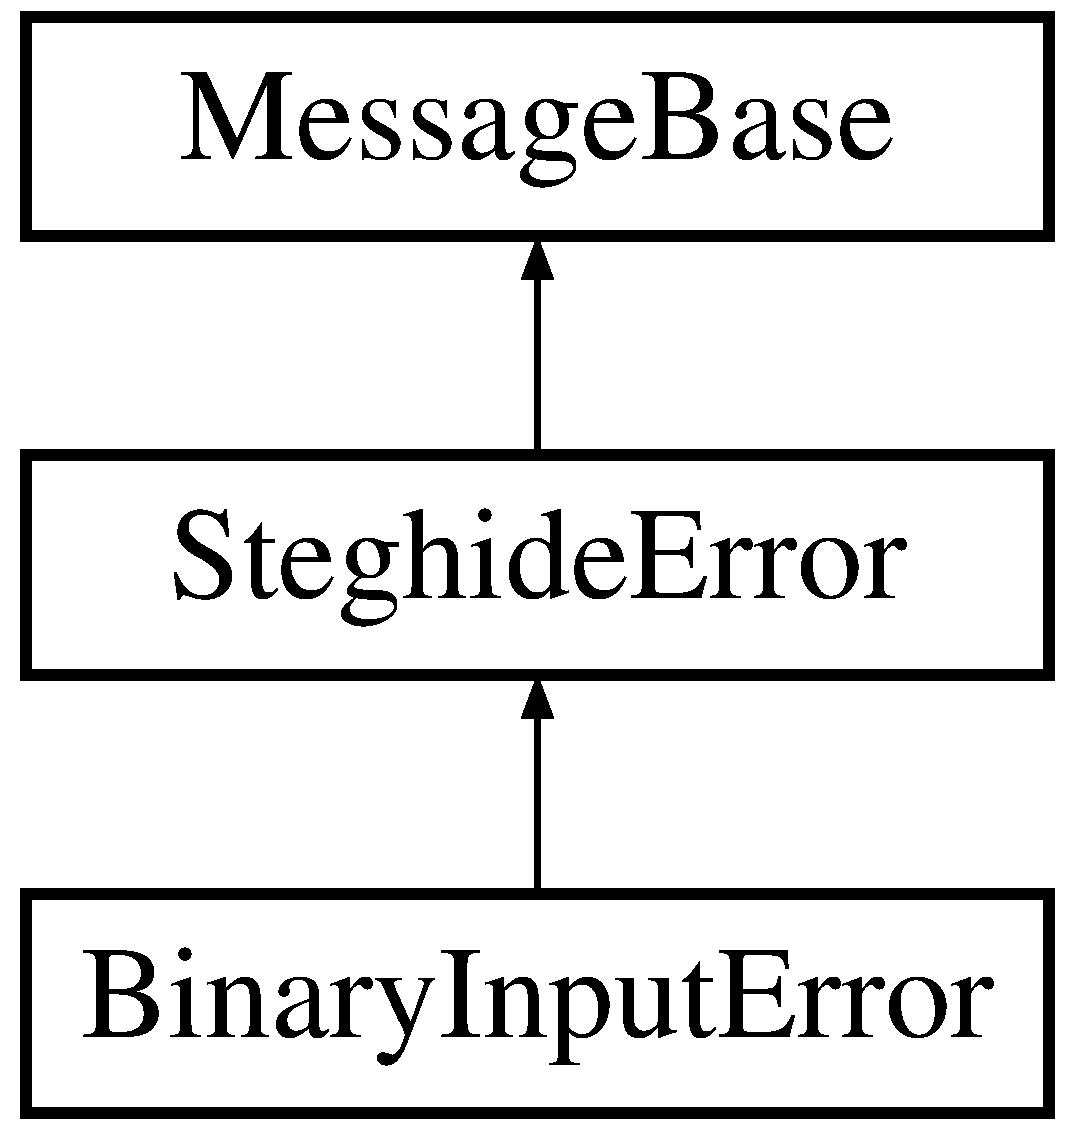
\includegraphics[height=3.000000cm]{classBinaryInputError}
\end{center}
\end{figure}
\subsection*{Public Types}
\begin{DoxyCompactItemize}
\item 
enum \textbf{ T\+Y\+PE} \{ \textbf{ F\+I\+L\+E\+\_\+\+E\+RR}, 
\textbf{ F\+I\+L\+E\+\_\+\+E\+OF}, 
\textbf{ S\+T\+D\+I\+N\+\_\+\+E\+RR}, 
\textbf{ S\+T\+D\+I\+N\+\_\+\+E\+OF}
 \}
\end{DoxyCompactItemize}
\subsection*{Public Member Functions}
\begin{DoxyCompactItemize}
\item 
\textbf{ Binary\+Input\+Error} (std\+::string fn, F\+I\+LE $\ast$s)
\item 
\textbf{ T\+Y\+PE} \textbf{ get\+Type} (void)
\end{DoxyCompactItemize}
\subsection*{Protected Member Functions}
\begin{DoxyCompactItemize}
\item 
void \textbf{ set\+Type} (\textbf{ T\+Y\+PE} t)
\end{DoxyCompactItemize}
\subsection*{Private Attributes}
\begin{DoxyCompactItemize}
\item 
\textbf{ T\+Y\+PE} \textbf{ type}
\end{DoxyCompactItemize}
\subsection*{Additional Inherited Members}


\subsection{Member Enumeration Documentation}
\mbox{\label{classBinaryInputError_a4000f1a2d7550997308b5180cd2c3b80}} 
\index{Binary\+Input\+Error@{Binary\+Input\+Error}!T\+Y\+PE@{T\+Y\+PE}}
\index{T\+Y\+PE@{T\+Y\+PE}!Binary\+Input\+Error@{Binary\+Input\+Error}}
\subsubsection{T\+Y\+PE}
{\footnotesize\ttfamily enum \textbf{ Binary\+Input\+Error\+::\+T\+Y\+PE}}

\begin{DoxyEnumFields}{Enumerator}
\raisebox{\heightof{T}}[0pt][0pt]{\index{F\+I\+L\+E\+\_\+\+E\+RR@{F\+I\+L\+E\+\_\+\+E\+RR}!Binary\+Input\+Error@{Binary\+Input\+Error}}\index{Binary\+Input\+Error@{Binary\+Input\+Error}!F\+I\+L\+E\+\_\+\+E\+RR@{F\+I\+L\+E\+\_\+\+E\+RR}}}\mbox{\label{classBinaryInputError_a4000f1a2d7550997308b5180cd2c3b80a68d5427b80ee64ff6c23c5b295c16a15}} 
F\+I\+L\+E\+\_\+\+E\+RR&\\
\hline

\raisebox{\heightof{T}}[0pt][0pt]{\index{F\+I\+L\+E\+\_\+\+E\+OF@{F\+I\+L\+E\+\_\+\+E\+OF}!Binary\+Input\+Error@{Binary\+Input\+Error}}\index{Binary\+Input\+Error@{Binary\+Input\+Error}!F\+I\+L\+E\+\_\+\+E\+OF@{F\+I\+L\+E\+\_\+\+E\+OF}}}\mbox{\label{classBinaryInputError_a4000f1a2d7550997308b5180cd2c3b80aa3a997b2c176c085657bfe9dc3a18820}} 
F\+I\+L\+E\+\_\+\+E\+OF&\\
\hline

\raisebox{\heightof{T}}[0pt][0pt]{\index{S\+T\+D\+I\+N\+\_\+\+E\+RR@{S\+T\+D\+I\+N\+\_\+\+E\+RR}!Binary\+Input\+Error@{Binary\+Input\+Error}}\index{Binary\+Input\+Error@{Binary\+Input\+Error}!S\+T\+D\+I\+N\+\_\+\+E\+RR@{S\+T\+D\+I\+N\+\_\+\+E\+RR}}}\mbox{\label{classBinaryInputError_a4000f1a2d7550997308b5180cd2c3b80a271275429fb38da06d7f1828962aafc2}} 
S\+T\+D\+I\+N\+\_\+\+E\+RR&\\
\hline

\raisebox{\heightof{T}}[0pt][0pt]{\index{S\+T\+D\+I\+N\+\_\+\+E\+OF@{S\+T\+D\+I\+N\+\_\+\+E\+OF}!Binary\+Input\+Error@{Binary\+Input\+Error}}\index{Binary\+Input\+Error@{Binary\+Input\+Error}!S\+T\+D\+I\+N\+\_\+\+E\+OF@{S\+T\+D\+I\+N\+\_\+\+E\+OF}}}\mbox{\label{classBinaryInputError_a4000f1a2d7550997308b5180cd2c3b80aa0b10e8c6660d29bd44920088e13b547}} 
S\+T\+D\+I\+N\+\_\+\+E\+OF&\\
\hline

\end{DoxyEnumFields}


\subsection{Constructor \& Destructor Documentation}
\mbox{\label{classBinaryInputError_a7b89b53504fd272f4af7ddbe74dea462}} 
\index{Binary\+Input\+Error@{Binary\+Input\+Error}!Binary\+Input\+Error@{Binary\+Input\+Error}}
\index{Binary\+Input\+Error@{Binary\+Input\+Error}!Binary\+Input\+Error@{Binary\+Input\+Error}}
\subsubsection{Binary\+Input\+Error()}
{\footnotesize\ttfamily Binary\+Input\+Error\+::\+Binary\+Input\+Error (\begin{DoxyParamCaption}\item[{std\+::string}]{fn,  }\item[{F\+I\+LE $\ast$}]{s }\end{DoxyParamCaption})}



\subsection{Member Function Documentation}
\mbox{\label{classBinaryInputError_a7dfcbc6c4b9cd7eeb2375a4d9edcd663}} 
\index{Binary\+Input\+Error@{Binary\+Input\+Error}!get\+Type@{get\+Type}}
\index{get\+Type@{get\+Type}!Binary\+Input\+Error@{Binary\+Input\+Error}}
\subsubsection{get\+Type()}
{\footnotesize\ttfamily \textbf{ Binary\+Input\+Error\+::\+T\+Y\+PE} Binary\+Input\+Error\+::get\+Type (\begin{DoxyParamCaption}\item[{void}]{ }\end{DoxyParamCaption})}

\mbox{\label{classBinaryInputError_a1b92b6969bbbab95f14d7222b9944515}} 
\index{Binary\+Input\+Error@{Binary\+Input\+Error}!set\+Type@{set\+Type}}
\index{set\+Type@{set\+Type}!Binary\+Input\+Error@{Binary\+Input\+Error}}
\subsubsection{set\+Type()}
{\footnotesize\ttfamily void Binary\+Input\+Error\+::set\+Type (\begin{DoxyParamCaption}\item[{\textbf{ Binary\+Input\+Error\+::\+T\+Y\+PE}}]{t }\end{DoxyParamCaption})\hspace{0.3cm}{\ttfamily [protected]}}



\subsection{Member Data Documentation}
\mbox{\label{classBinaryInputError_aad5342bc5ab9fb78cc72818505aaed97}} 
\index{Binary\+Input\+Error@{Binary\+Input\+Error}!type@{type}}
\index{type@{type}!Binary\+Input\+Error@{Binary\+Input\+Error}}
\subsubsection{type}
{\footnotesize\ttfamily \textbf{ T\+Y\+PE} Binary\+Input\+Error\+::type\hspace{0.3cm}{\ttfamily [private]}}



The documentation for this class was generated from the following files\+:\begin{DoxyCompactItemize}
\item 
\textbf{ error.\+h}\item 
\textbf{ error.\+cc}\end{DoxyCompactItemize}

\section{Binary\+IO Class Reference}
\label{classBinaryIO}\index{Binary\+IO@{Binary\+IO}}


provides methods for file i/o as needed by the rest of steghide  




{\ttfamily \#include $<$Binary\+I\+O.\+h$>$}

\subsection*{Public Types}
\begin{DoxyCompactItemize}
\item 
enum \textbf{ M\+O\+DE} \{ \textbf{ R\+E\+AD}, 
\textbf{ W\+R\+I\+TE}
 \}
\end{DoxyCompactItemize}
\subsection*{Public Member Functions}
\begin{DoxyCompactItemize}
\item 
\textbf{ Binary\+IO} (void)
\item 
\textbf{ Binary\+IO} (const std\+::string \&fn, \textbf{ M\+O\+DE} m)
\item 
\textbf{ $\sim$\+Binary\+IO} (void)
\item 
const std\+::string \& \textbf{ get\+Name} (void) const
\item 
bool \textbf{ is\+\_\+open} (void) const
\item 
bool \textbf{ is\+\_\+std} (void) const
\item 
unsigned long \textbf{ get\+Pos} (void) const
\item 
bool \textbf{ eof} (void) const
\item 
void \textbf{ open} (const std\+::string \&fn, \textbf{ M\+O\+DE} m)
\item 
void \textbf{ close} (void)
\item 
\textbf{ B\+Y\+TE} \textbf{ read8} (void)
\item 
\textbf{ U\+W\+O\+R\+D16} \textbf{ read16\+\_\+le} (void)
\item 
\textbf{ U\+W\+O\+R\+D16} \textbf{ read16\+\_\+be} (void)
\item 
\textbf{ U\+W\+O\+R\+D32} \textbf{ read32\+\_\+le} (void)
\item 
\textbf{ U\+W\+O\+R\+D32} \textbf{ read32\+\_\+be} (void)
\item 
\textbf{ U\+W\+O\+R\+D32} \textbf{ read\+\_\+le} (unsigned short n)
\item 
std\+::string \textbf{ readstring} (unsigned int len)
\item 
void \textbf{ write8} (\textbf{ B\+Y\+TE} val)
\item 
void \textbf{ write16\+\_\+le} (\textbf{ U\+W\+O\+R\+D16} val)
\item 
void \textbf{ write16\+\_\+be} (\textbf{ U\+W\+O\+R\+D16} val)
\item 
void \textbf{ write32\+\_\+le} (\textbf{ U\+W\+O\+R\+D32} val)
\item 
void \textbf{ write32\+\_\+be} (\textbf{ U\+W\+O\+R\+D32} val)
\item 
void \textbf{ write\+\_\+le} (\textbf{ U\+W\+O\+R\+D32} val, unsigned short n)
\item 
void \textbf{ writestring} (const std\+::string \&s)
\item 
F\+I\+LE $\ast$ \textbf{ get\+Stream} (void) const
\end{DoxyCompactItemize}
\subsection*{Protected Member Functions}
\begin{DoxyCompactItemize}
\item 
void \textbf{ set\+Stream} (F\+I\+LE $\ast$s)
\item 
void \textbf{ set\+Name} (const std\+::string \&fn)
\item 
\textbf{ M\+O\+DE} \textbf{ get\+Mode} (void) const
\item 
void \textbf{ set\+Mode} (\textbf{ M\+O\+DE} m)
\end{DoxyCompactItemize}
\subsection*{Private Member Functions}
\begin{DoxyCompactItemize}
\item 
void \textbf{ init} (void)
\item 
void \textbf{ set\+\_\+open} (bool o)
\item 
void \textbf{ check\+Force} (const std\+::string \&fn) const
\item 
bool \textbf{ Fileexists} (const std\+::string \&fn) const
\end{DoxyCompactItemize}
\subsection*{Private Attributes}
\begin{DoxyCompactItemize}
\item 
std\+::string \textbf{ Name}
\item 
F\+I\+LE $\ast$ \textbf{ Stream}
\item 
bool \textbf{ File\+Open}
\item 
\textbf{ M\+O\+DE} \textbf{ Mode}
\end{DoxyCompactItemize}


\subsection{Member Enumeration Documentation}
\mbox{\label{classBinaryIO_a39efef0fa56b45a901763f0f9d1515f8}} 
\index{Binary\+IO@{Binary\+IO}!M\+O\+DE@{M\+O\+DE}}
\index{M\+O\+DE@{M\+O\+DE}!Binary\+IO@{Binary\+IO}}
\subsubsection{M\+O\+DE}
{\footnotesize\ttfamily enum \textbf{ Binary\+I\+O\+::\+M\+O\+DE}}

\begin{DoxyEnumFields}{Enumerator}
\raisebox{\heightof{T}}[0pt][0pt]{\index{R\+E\+AD@{R\+E\+AD}!Binary\+IO@{Binary\+IO}}\index{Binary\+IO@{Binary\+IO}!R\+E\+AD@{R\+E\+AD}}}\mbox{\label{classBinaryIO_a39efef0fa56b45a901763f0f9d1515f8aab09be55cd7e94f751c2e7fabb33608a}} 
R\+E\+AD&\\
\hline

\raisebox{\heightof{T}}[0pt][0pt]{\index{W\+R\+I\+TE@{W\+R\+I\+TE}!Binary\+IO@{Binary\+IO}}\index{Binary\+IO@{Binary\+IO}!W\+R\+I\+TE@{W\+R\+I\+TE}}}\mbox{\label{classBinaryIO_a39efef0fa56b45a901763f0f9d1515f8a58e070ce9ef4f5b02b7f65a7326b22d2}} 
W\+R\+I\+TE&\\
\hline

\end{DoxyEnumFields}


\subsection{Constructor \& Destructor Documentation}
\mbox{\label{classBinaryIO_a0bf35fbb43ff17d5b0a29bd492acd209}} 
\index{Binary\+IO@{Binary\+IO}!Binary\+IO@{Binary\+IO}}
\index{Binary\+IO@{Binary\+IO}!Binary\+IO@{Binary\+IO}}
\subsubsection{Binary\+I\+O()\hspace{0.1cm}{\footnotesize\ttfamily [1/2]}}
{\footnotesize\ttfamily Binary\+I\+O\+::\+Binary\+IO (\begin{DoxyParamCaption}\item[{void}]{ }\end{DoxyParamCaption})}

\mbox{\label{classBinaryIO_a7ccae332f41b5437506d6cb58e0e6309}} 
\index{Binary\+IO@{Binary\+IO}!Binary\+IO@{Binary\+IO}}
\index{Binary\+IO@{Binary\+IO}!Binary\+IO@{Binary\+IO}}
\subsubsection{Binary\+I\+O()\hspace{0.1cm}{\footnotesize\ttfamily [2/2]}}
{\footnotesize\ttfamily Binary\+I\+O\+::\+Binary\+IO (\begin{DoxyParamCaption}\item[{const std\+::string \&}]{fn,  }\item[{\textbf{ M\+O\+DE}}]{m }\end{DoxyParamCaption})}

construct a \doxyref{Binary\+IO}{p.}{classBinaryIO} object 
\begin{DoxyParams}{Parameters}
{\em fn} & the filename (\char`\"{}\char`\"{} to indicate stdin/stdout) \\
\hline
{\em m} & the mode (\doxyref{Binary\+I\+O\+::\+R\+E\+AD}{p.}{classBinaryIO_a39efef0fa56b45a901763f0f9d1515f8aab09be55cd7e94f751c2e7fabb33608a} or \doxyref{Binary\+I\+O\+::\+W\+R\+I\+TE}{p.}{classBinaryIO_a39efef0fa56b45a901763f0f9d1515f8a58e070ce9ef4f5b02b7f65a7326b22d2})\\
\hline
\end{DoxyParams}
The file described by fn is opened in the given mode. \mbox{\label{classBinaryIO_a998ac3108e4a6a0bbb97b6488b85d279}} 
\index{Binary\+IO@{Binary\+IO}!````~Binary\+IO@{$\sim$\+Binary\+IO}}
\index{````~Binary\+IO@{$\sim$\+Binary\+IO}!Binary\+IO@{Binary\+IO}}
\subsubsection{$\sim$\+Binary\+I\+O()}
{\footnotesize\ttfamily Binary\+I\+O\+::$\sim$\+Binary\+IO (\begin{DoxyParamCaption}\item[{void}]{ }\end{DoxyParamCaption})}



\subsection{Member Function Documentation}
\mbox{\label{classBinaryIO_aead6fb65e7d2c70fb5a65d4483fa456a}} 
\index{Binary\+IO@{Binary\+IO}!check\+Force@{check\+Force}}
\index{check\+Force@{check\+Force}!Binary\+IO@{Binary\+IO}}
\subsubsection{check\+Force()}
{\footnotesize\ttfamily void Binary\+I\+O\+::check\+Force (\begin{DoxyParamCaption}\item[{const std\+::string \&}]{fn }\end{DoxyParamCaption}) const\hspace{0.3cm}{\ttfamily [private]}}

when opening a file in write mode perform various checks depending on the value of the force argument \mbox{\label{classBinaryIO_a7d1b96a2c17fb45e7918e6d730861d04}} 
\index{Binary\+IO@{Binary\+IO}!close@{close}}
\index{close@{close}!Binary\+IO@{Binary\+IO}}
\subsubsection{close()}
{\footnotesize\ttfamily void Binary\+I\+O\+::close (\begin{DoxyParamCaption}\item[{void}]{ }\end{DoxyParamCaption})}

close the currently open file -\/ it is save to call \doxyref{close()}{p.}{classBinaryIO_a7d1b96a2c17fb45e7918e6d730861d04} even if \doxyref{is\+\_\+std()}{p.}{classBinaryIO_a7d40c1b945ac9bf34f1187fd315b33ab} is true \mbox{\label{classBinaryIO_a4b3115d6947100fc9171160c6beab7d1}} 
\index{Binary\+IO@{Binary\+IO}!eof@{eof}}
\index{eof@{eof}!Binary\+IO@{Binary\+IO}}
\subsubsection{eof()}
{\footnotesize\ttfamily bool Binary\+I\+O\+::eof (\begin{DoxyParamCaption}\item[{void}]{ }\end{DoxyParamCaption}) const}

is the current state of this file at the end of the file \mbox{\label{classBinaryIO_aca30a749adb6f750011a70e9e0e40802}} 
\index{Binary\+IO@{Binary\+IO}!Fileexists@{Fileexists}}
\index{Fileexists@{Fileexists}!Binary\+IO@{Binary\+IO}}
\subsubsection{Fileexists()}
{\footnotesize\ttfamily bool Binary\+I\+O\+::\+Fileexists (\begin{DoxyParamCaption}\item[{const std\+::string \&}]{fn }\end{DoxyParamCaption}) const\hspace{0.3cm}{\ttfamily [private]}}

check if the file described by fn exists \begin{DoxyReturn}{Returns}
true iff a fopen call with fn as file name succeeded 
\end{DoxyReturn}
\mbox{\label{classBinaryIO_a08ba7230d2ba5b866bbd78b024b10de9}} 
\index{Binary\+IO@{Binary\+IO}!get\+Mode@{get\+Mode}}
\index{get\+Mode@{get\+Mode}!Binary\+IO@{Binary\+IO}}
\subsubsection{get\+Mode()}
{\footnotesize\ttfamily \textbf{ M\+O\+DE} Binary\+I\+O\+::get\+Mode (\begin{DoxyParamCaption}\item[{void}]{ }\end{DoxyParamCaption}) const\hspace{0.3cm}{\ttfamily [inline]}, {\ttfamily [protected]}}

\mbox{\label{classBinaryIO_abad253f71b8705a2315d4d9a3dfdc080}} 
\index{Binary\+IO@{Binary\+IO}!get\+Name@{get\+Name}}
\index{get\+Name@{get\+Name}!Binary\+IO@{Binary\+IO}}
\subsubsection{get\+Name()}
{\footnotesize\ttfamily const std\+::string\& Binary\+I\+O\+::get\+Name (\begin{DoxyParamCaption}\item[{void}]{ }\end{DoxyParamCaption}) const\hspace{0.3cm}{\ttfamily [inline]}}

get the name (with path) of this file \mbox{\label{classBinaryIO_a3a31f0549a7effe9aeec868b4acd36db}} 
\index{Binary\+IO@{Binary\+IO}!get\+Pos@{get\+Pos}}
\index{get\+Pos@{get\+Pos}!Binary\+IO@{Binary\+IO}}
\subsubsection{get\+Pos()}
{\footnotesize\ttfamily unsigned long Binary\+I\+O\+::get\+Pos (\begin{DoxyParamCaption}\item[{void}]{ }\end{DoxyParamCaption}) const\hspace{0.3cm}{\ttfamily [inline]}}

get the current position in the current file \mbox{\label{classBinaryIO_a82b8e015444d4f08409266aba8409cad}} 
\index{Binary\+IO@{Binary\+IO}!get\+Stream@{get\+Stream}}
\index{get\+Stream@{get\+Stream}!Binary\+IO@{Binary\+IO}}
\subsubsection{get\+Stream()}
{\footnotesize\ttfamily F\+I\+LE$\ast$ Binary\+I\+O\+::get\+Stream (\begin{DoxyParamCaption}\item[{void}]{ }\end{DoxyParamCaption}) const\hspace{0.3cm}{\ttfamily [inline]}}

get the underlying cstdio F\+I\+L\+E$\ast$ pointer \mbox{\label{classBinaryIO_ae17f9a27379768a7403fde20b4b5f660}} 
\index{Binary\+IO@{Binary\+IO}!init@{init}}
\index{init@{init}!Binary\+IO@{Binary\+IO}}
\subsubsection{init()}
{\footnotesize\ttfamily void Binary\+I\+O\+::init (\begin{DoxyParamCaption}\item[{void}]{ }\end{DoxyParamCaption})\hspace{0.3cm}{\ttfamily [private]}}

\mbox{\label{classBinaryIO_ad01391d8b01b14dc524036e61194cd30}} 
\index{Binary\+IO@{Binary\+IO}!is\+\_\+open@{is\+\_\+open}}
\index{is\+\_\+open@{is\+\_\+open}!Binary\+IO@{Binary\+IO}}
\subsubsection{is\+\_\+open()}
{\footnotesize\ttfamily bool Binary\+I\+O\+::is\+\_\+open (\begin{DoxyParamCaption}\item[{void}]{ }\end{DoxyParamCaption}) const\hspace{0.3cm}{\ttfamily [inline]}}

is this file currently opened ? \mbox{\label{classBinaryIO_a7d40c1b945ac9bf34f1187fd315b33ab}} 
\index{Binary\+IO@{Binary\+IO}!is\+\_\+std@{is\+\_\+std}}
\index{is\+\_\+std@{is\+\_\+std}!Binary\+IO@{Binary\+IO}}
\subsubsection{is\+\_\+std()}
{\footnotesize\ttfamily bool Binary\+I\+O\+::is\+\_\+std (\begin{DoxyParamCaption}\item[{void}]{ }\end{DoxyParamCaption}) const\hspace{0.3cm}{\ttfamily [inline]}}

is this file a standard stream (stdin or stdout) ? \mbox{\label{classBinaryIO_a789dc643814786b49bdd0ab0484b7218}} 
\index{Binary\+IO@{Binary\+IO}!open@{open}}
\index{open@{open}!Binary\+IO@{Binary\+IO}}
\subsubsection{open()}
{\footnotesize\ttfamily void Binary\+I\+O\+::open (\begin{DoxyParamCaption}\item[{const std\+::string \&}]{fn,  }\item[{\textbf{ M\+O\+DE}}]{m }\end{DoxyParamCaption})}

open the file given by fn in the mode m 
\begin{DoxyParams}{Parameters}
{\em fn} & a filename (\char`\"{}\char`\"{} to indicate stdin/stdout) \\
\hline
{\em m} & the mode (\doxyref{Binary\+I\+O\+::\+R\+E\+AD}{p.}{classBinaryIO_a39efef0fa56b45a901763f0f9d1515f8aab09be55cd7e94f751c2e7fabb33608a} or \doxyref{Binary\+I\+O\+::\+W\+R\+I\+TE}{p.}{classBinaryIO_a39efef0fa56b45a901763f0f9d1515f8a58e070ce9ef4f5b02b7f65a7326b22d2}) \\
\hline
\end{DoxyParams}
\mbox{\label{classBinaryIO_ae6cab3a9995c04305f22e716ba20c332}} 
\index{Binary\+IO@{Binary\+IO}!read16\+\_\+be@{read16\+\_\+be}}
\index{read16\+\_\+be@{read16\+\_\+be}!Binary\+IO@{Binary\+IO}}
\subsubsection{read16\+\_\+be()}
{\footnotesize\ttfamily \textbf{ U\+W\+O\+R\+D16} Binary\+I\+O\+::read16\+\_\+be (\begin{DoxyParamCaption}\item[{void}]{ }\end{DoxyParamCaption})}

read two bytes from the file using big-\/endian byte ordering \mbox{\label{classBinaryIO_a9af2449937a4c50c638be6c03815a0cf}} 
\index{Binary\+IO@{Binary\+IO}!read16\+\_\+le@{read16\+\_\+le}}
\index{read16\+\_\+le@{read16\+\_\+le}!Binary\+IO@{Binary\+IO}}
\subsubsection{read16\+\_\+le()}
{\footnotesize\ttfamily \textbf{ U\+W\+O\+R\+D16} Binary\+I\+O\+::read16\+\_\+le (\begin{DoxyParamCaption}\item[{void}]{ }\end{DoxyParamCaption})}

read two bytes from the file using little-\/endian byte ordering \mbox{\label{classBinaryIO_a5f48a7aacb83a7381d9ce67f49d3a36c}} 
\index{Binary\+IO@{Binary\+IO}!read32\+\_\+be@{read32\+\_\+be}}
\index{read32\+\_\+be@{read32\+\_\+be}!Binary\+IO@{Binary\+IO}}
\subsubsection{read32\+\_\+be()}
{\footnotesize\ttfamily \textbf{ U\+W\+O\+R\+D32} Binary\+I\+O\+::read32\+\_\+be (\begin{DoxyParamCaption}\item[{void}]{ }\end{DoxyParamCaption})}

read four bytes from the file using big-\/endian byte ordering \mbox{\label{classBinaryIO_a41541700c43a89efd9a4e73bc0cb7bb7}} 
\index{Binary\+IO@{Binary\+IO}!read32\+\_\+le@{read32\+\_\+le}}
\index{read32\+\_\+le@{read32\+\_\+le}!Binary\+IO@{Binary\+IO}}
\subsubsection{read32\+\_\+le()}
{\footnotesize\ttfamily \textbf{ U\+W\+O\+R\+D32} Binary\+I\+O\+::read32\+\_\+le (\begin{DoxyParamCaption}\item[{void}]{ }\end{DoxyParamCaption})}

read four bytes from the file using little-\/endian byte ordering \mbox{\label{classBinaryIO_a23502610cfdf0d789dc02ef16262dbe1}} 
\index{Binary\+IO@{Binary\+IO}!read8@{read8}}
\index{read8@{read8}!Binary\+IO@{Binary\+IO}}
\subsubsection{read8()}
{\footnotesize\ttfamily \textbf{ B\+Y\+TE} Binary\+I\+O\+::read8 (\begin{DoxyParamCaption}\item[{void}]{ }\end{DoxyParamCaption})}

read one byte from the file \mbox{\label{classBinaryIO_a320263cd4adaee51b1ae982bdb3b6615}} 
\index{Binary\+IO@{Binary\+IO}!read\+\_\+le@{read\+\_\+le}}
\index{read\+\_\+le@{read\+\_\+le}!Binary\+IO@{Binary\+IO}}
\subsubsection{read\+\_\+le()}
{\footnotesize\ttfamily \textbf{ U\+W\+O\+R\+D32} Binary\+I\+O\+::read\+\_\+le (\begin{DoxyParamCaption}\item[{unsigned short}]{n }\end{DoxyParamCaption})}

read n bytes (little endian byte ordering) 
\begin{DoxyParams}{Parameters}
{\em n} & the number of bytes to read (must be $<$= 4) \\
\hline
\end{DoxyParams}
\mbox{\label{classBinaryIO_a02f7eaa184af4082dd438a5fcd2c318b}} 
\index{Binary\+IO@{Binary\+IO}!readstring@{readstring}}
\index{readstring@{readstring}!Binary\+IO@{Binary\+IO}}
\subsubsection{readstring()}
{\footnotesize\ttfamily std\+::string Binary\+I\+O\+::readstring (\begin{DoxyParamCaption}\item[{unsigned int}]{len }\end{DoxyParamCaption})}

read a string with length len from the file \mbox{\label{classBinaryIO_aefffa46734a984085cd4309939bcaddb}} 
\index{Binary\+IO@{Binary\+IO}!set\+\_\+open@{set\+\_\+open}}
\index{set\+\_\+open@{set\+\_\+open}!Binary\+IO@{Binary\+IO}}
\subsubsection{set\+\_\+open()}
{\footnotesize\ttfamily void Binary\+I\+O\+::set\+\_\+open (\begin{DoxyParamCaption}\item[{bool}]{o }\end{DoxyParamCaption})\hspace{0.3cm}{\ttfamily [inline]}, {\ttfamily [private]}}

\mbox{\label{classBinaryIO_abea111493f6008e396e4f99924912c7b}} 
\index{Binary\+IO@{Binary\+IO}!set\+Mode@{set\+Mode}}
\index{set\+Mode@{set\+Mode}!Binary\+IO@{Binary\+IO}}
\subsubsection{set\+Mode()}
{\footnotesize\ttfamily void Binary\+I\+O\+::set\+Mode (\begin{DoxyParamCaption}\item[{\textbf{ M\+O\+DE}}]{m }\end{DoxyParamCaption})\hspace{0.3cm}{\ttfamily [inline]}, {\ttfamily [protected]}}

\mbox{\label{classBinaryIO_a9c866c14899279ad6e9fabb6b69767d5}} 
\index{Binary\+IO@{Binary\+IO}!set\+Name@{set\+Name}}
\index{set\+Name@{set\+Name}!Binary\+IO@{Binary\+IO}}
\subsubsection{set\+Name()}
{\footnotesize\ttfamily void Binary\+I\+O\+::set\+Name (\begin{DoxyParamCaption}\item[{const std\+::string \&}]{fn }\end{DoxyParamCaption})\hspace{0.3cm}{\ttfamily [inline]}, {\ttfamily [protected]}}

\mbox{\label{classBinaryIO_a54eb9e307df74443779107b2fe772bbf}} 
\index{Binary\+IO@{Binary\+IO}!set\+Stream@{set\+Stream}}
\index{set\+Stream@{set\+Stream}!Binary\+IO@{Binary\+IO}}
\subsubsection{set\+Stream()}
{\footnotesize\ttfamily void Binary\+I\+O\+::set\+Stream (\begin{DoxyParamCaption}\item[{F\+I\+LE $\ast$}]{s }\end{DoxyParamCaption})\hspace{0.3cm}{\ttfamily [inline]}, {\ttfamily [protected]}}

\mbox{\label{classBinaryIO_ac551a0c15a8027b830d461df36c70982}} 
\index{Binary\+IO@{Binary\+IO}!write16\+\_\+be@{write16\+\_\+be}}
\index{write16\+\_\+be@{write16\+\_\+be}!Binary\+IO@{Binary\+IO}}
\subsubsection{write16\+\_\+be()}
{\footnotesize\ttfamily void Binary\+I\+O\+::write16\+\_\+be (\begin{DoxyParamCaption}\item[{\textbf{ U\+W\+O\+R\+D16}}]{val }\end{DoxyParamCaption})}

write two bytes to the file using big-\/endian byte ordering \mbox{\label{classBinaryIO_af029be6769535da614986f3625d24c60}} 
\index{Binary\+IO@{Binary\+IO}!write16\+\_\+le@{write16\+\_\+le}}
\index{write16\+\_\+le@{write16\+\_\+le}!Binary\+IO@{Binary\+IO}}
\subsubsection{write16\+\_\+le()}
{\footnotesize\ttfamily void Binary\+I\+O\+::write16\+\_\+le (\begin{DoxyParamCaption}\item[{\textbf{ U\+W\+O\+R\+D16}}]{val }\end{DoxyParamCaption})}

write two bytes to the file using little-\/endian byte ordering \mbox{\label{classBinaryIO_a778cb8560b7792e96a8de7a32440e2fe}} 
\index{Binary\+IO@{Binary\+IO}!write32\+\_\+be@{write32\+\_\+be}}
\index{write32\+\_\+be@{write32\+\_\+be}!Binary\+IO@{Binary\+IO}}
\subsubsection{write32\+\_\+be()}
{\footnotesize\ttfamily void Binary\+I\+O\+::write32\+\_\+be (\begin{DoxyParamCaption}\item[{\textbf{ U\+W\+O\+R\+D32}}]{val }\end{DoxyParamCaption})}

write four bytes to the file using big-\/endian byte ordering \mbox{\label{classBinaryIO_a546779c9f2bd7a3bce516310605cfbb0}} 
\index{Binary\+IO@{Binary\+IO}!write32\+\_\+le@{write32\+\_\+le}}
\index{write32\+\_\+le@{write32\+\_\+le}!Binary\+IO@{Binary\+IO}}
\subsubsection{write32\+\_\+le()}
{\footnotesize\ttfamily void Binary\+I\+O\+::write32\+\_\+le (\begin{DoxyParamCaption}\item[{\textbf{ U\+W\+O\+R\+D32}}]{val }\end{DoxyParamCaption})}

write four bytes to the file using little-\/endian byte ordering \mbox{\label{classBinaryIO_a3df966cbb5955a9cc12db9c1b841f316}} 
\index{Binary\+IO@{Binary\+IO}!write8@{write8}}
\index{write8@{write8}!Binary\+IO@{Binary\+IO}}
\subsubsection{write8()}
{\footnotesize\ttfamily void Binary\+I\+O\+::write8 (\begin{DoxyParamCaption}\item[{\textbf{ B\+Y\+TE}}]{val }\end{DoxyParamCaption})}

write one byte to the file \mbox{\label{classBinaryIO_a6d8356e8fbf862d79d8ec97fb93217c3}} 
\index{Binary\+IO@{Binary\+IO}!write\+\_\+le@{write\+\_\+le}}
\index{write\+\_\+le@{write\+\_\+le}!Binary\+IO@{Binary\+IO}}
\subsubsection{write\+\_\+le()}
{\footnotesize\ttfamily void Binary\+I\+O\+::write\+\_\+le (\begin{DoxyParamCaption}\item[{\textbf{ U\+W\+O\+R\+D32}}]{val,  }\item[{unsigned short}]{n }\end{DoxyParamCaption})}

write n bytes of val (little endian byte ordering) 
\begin{DoxyParams}{Parameters}
{\em n} & the number of bytes to write (must be $<$= 4) \\
\hline
{\em val} & the value \\
\hline
\end{DoxyParams}
\mbox{\label{classBinaryIO_a116ca944bd525917198f8438c9c2f1a1}} 
\index{Binary\+IO@{Binary\+IO}!writestring@{writestring}}
\index{writestring@{writestring}!Binary\+IO@{Binary\+IO}}
\subsubsection{writestring()}
{\footnotesize\ttfamily void Binary\+I\+O\+::writestring (\begin{DoxyParamCaption}\item[{const std\+::string \&}]{s }\end{DoxyParamCaption})}



\subsection{Member Data Documentation}
\mbox{\label{classBinaryIO_ac9ae8526d944e3e26f50618afe09d3ab}} 
\index{Binary\+IO@{Binary\+IO}!File\+Open@{File\+Open}}
\index{File\+Open@{File\+Open}!Binary\+IO@{Binary\+IO}}
\subsubsection{File\+Open}
{\footnotesize\ttfamily bool Binary\+I\+O\+::\+File\+Open\hspace{0.3cm}{\ttfamily [private]}}

\mbox{\label{classBinaryIO_aa3305696bab79bc4e3b18ea6bfff4477}} 
\index{Binary\+IO@{Binary\+IO}!Mode@{Mode}}
\index{Mode@{Mode}!Binary\+IO@{Binary\+IO}}
\subsubsection{Mode}
{\footnotesize\ttfamily \textbf{ M\+O\+DE} Binary\+I\+O\+::\+Mode\hspace{0.3cm}{\ttfamily [private]}}

\mbox{\label{classBinaryIO_aecedcd5d40e7b4326cd2ef3aa0e3c2ad}} 
\index{Binary\+IO@{Binary\+IO}!Name@{Name}}
\index{Name@{Name}!Binary\+IO@{Binary\+IO}}
\subsubsection{Name}
{\footnotesize\ttfamily std\+::string Binary\+I\+O\+::\+Name\hspace{0.3cm}{\ttfamily [private]}}

\mbox{\label{classBinaryIO_aa0009cff8318597b0c46a339d38f08ce}} 
\index{Binary\+IO@{Binary\+IO}!Stream@{Stream}}
\index{Stream@{Stream}!Binary\+IO@{Binary\+IO}}
\subsubsection{Stream}
{\footnotesize\ttfamily F\+I\+LE$\ast$ Binary\+I\+O\+::\+Stream\hspace{0.3cm}{\ttfamily [private]}}



The documentation for this class was generated from the following files\+:\begin{DoxyCompactItemize}
\item 
\textbf{ Binary\+I\+O.\+h}\item 
\textbf{ Binary\+I\+O.\+cc}\end{DoxyCompactItemize}

\section{Binary\+Output\+Error Class Reference}
\label{classBinaryOutputError}\index{Binary\+Output\+Error@{Binary\+Output\+Error}}


{\ttfamily \#include $<$error.\+h$>$}

Inheritance diagram for Binary\+Output\+Error\+:\begin{figure}[H]
\begin{center}
\leavevmode
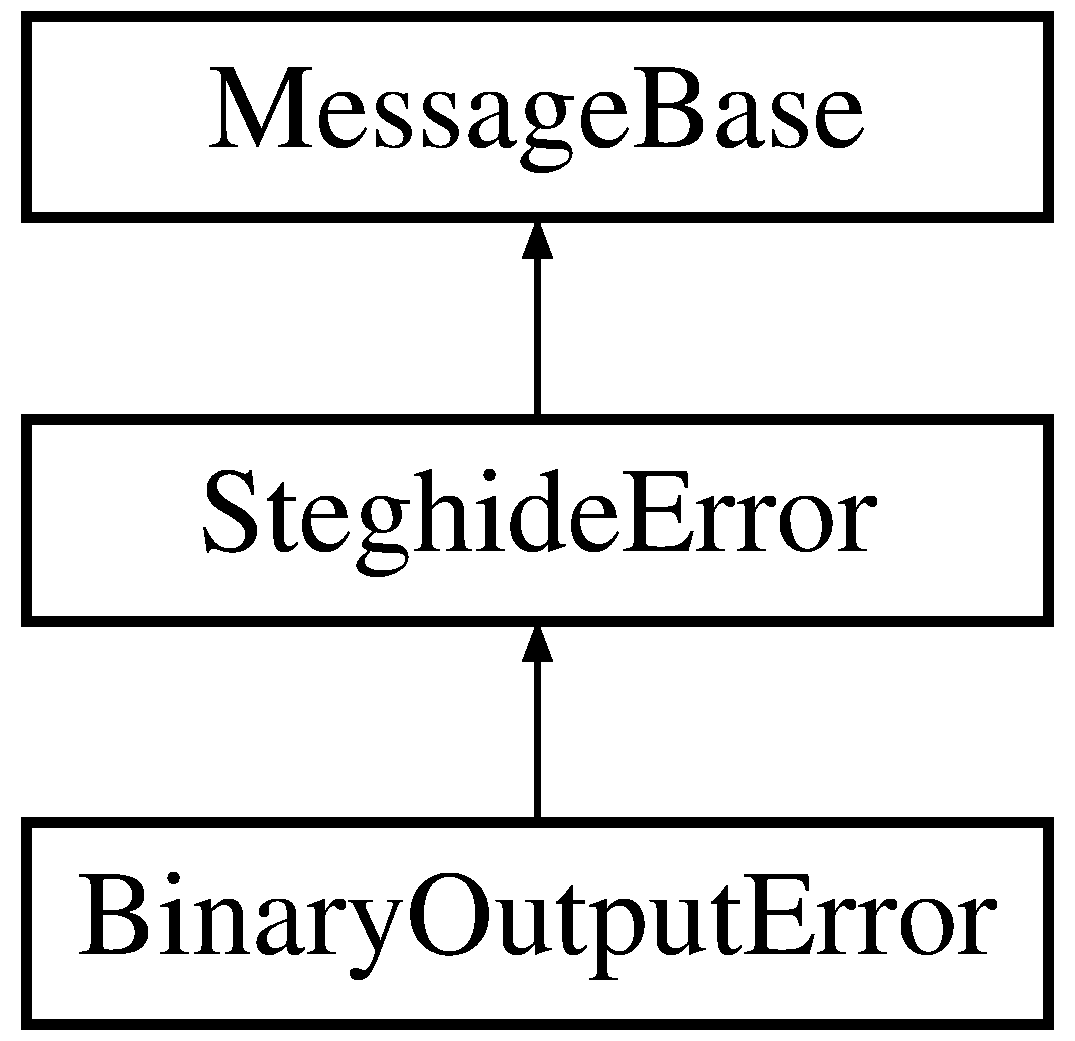
\includegraphics[height=3.000000cm]{classBinaryOutputError}
\end{center}
\end{figure}
\subsection*{Public Types}
\begin{DoxyCompactItemize}
\item 
enum \textbf{ T\+Y\+PE} \{ \textbf{ F\+I\+L\+E\+\_\+\+E\+RR}, 
\textbf{ S\+T\+D\+O\+U\+T\+\_\+\+E\+RR}
 \}
\end{DoxyCompactItemize}
\subsection*{Public Member Functions}
\begin{DoxyCompactItemize}
\item 
\textbf{ Binary\+Output\+Error} (std\+::string fn)
\item 
\textbf{ T\+Y\+PE} \textbf{ get\+Type} (void)
\end{DoxyCompactItemize}
\subsection*{Protected Member Functions}
\begin{DoxyCompactItemize}
\item 
void \textbf{ set\+Type} (\textbf{ T\+Y\+PE} t)
\end{DoxyCompactItemize}
\subsection*{Private Attributes}
\begin{DoxyCompactItemize}
\item 
\textbf{ T\+Y\+PE} \textbf{ type}
\end{DoxyCompactItemize}
\subsection*{Additional Inherited Members}


\subsection{Member Enumeration Documentation}
\mbox{\label{classBinaryOutputError_a7b16a5e7bb3efac8bd37555a1da4db6c}} 
\index{Binary\+Output\+Error@{Binary\+Output\+Error}!T\+Y\+PE@{T\+Y\+PE}}
\index{T\+Y\+PE@{T\+Y\+PE}!Binary\+Output\+Error@{Binary\+Output\+Error}}
\subsubsection{T\+Y\+PE}
{\footnotesize\ttfamily enum \textbf{ Binary\+Output\+Error\+::\+T\+Y\+PE}}

\begin{DoxyEnumFields}{Enumerator}
\raisebox{\heightof{T}}[0pt][0pt]{\index{F\+I\+L\+E\+\_\+\+E\+RR@{F\+I\+L\+E\+\_\+\+E\+RR}!Binary\+Output\+Error@{Binary\+Output\+Error}}\index{Binary\+Output\+Error@{Binary\+Output\+Error}!F\+I\+L\+E\+\_\+\+E\+RR@{F\+I\+L\+E\+\_\+\+E\+RR}}}\mbox{\label{classBinaryOutputError_a7b16a5e7bb3efac8bd37555a1da4db6caaa6585014f63247bc991e256c76fa1fa}} 
F\+I\+L\+E\+\_\+\+E\+RR&\\
\hline

\raisebox{\heightof{T}}[0pt][0pt]{\index{S\+T\+D\+O\+U\+T\+\_\+\+E\+RR@{S\+T\+D\+O\+U\+T\+\_\+\+E\+RR}!Binary\+Output\+Error@{Binary\+Output\+Error}}\index{Binary\+Output\+Error@{Binary\+Output\+Error}!S\+T\+D\+O\+U\+T\+\_\+\+E\+RR@{S\+T\+D\+O\+U\+T\+\_\+\+E\+RR}}}\mbox{\label{classBinaryOutputError_a7b16a5e7bb3efac8bd37555a1da4db6ca67dab9937d3cf0e71109946f73d53b3f}} 
S\+T\+D\+O\+U\+T\+\_\+\+E\+RR&\\
\hline

\end{DoxyEnumFields}


\subsection{Constructor \& Destructor Documentation}
\mbox{\label{classBinaryOutputError_a401d62a6882f3caf9423e7f1e0131522}} 
\index{Binary\+Output\+Error@{Binary\+Output\+Error}!Binary\+Output\+Error@{Binary\+Output\+Error}}
\index{Binary\+Output\+Error@{Binary\+Output\+Error}!Binary\+Output\+Error@{Binary\+Output\+Error}}
\subsubsection{Binary\+Output\+Error()}
{\footnotesize\ttfamily Binary\+Output\+Error\+::\+Binary\+Output\+Error (\begin{DoxyParamCaption}\item[{std\+::string}]{fn }\end{DoxyParamCaption})}



\subsection{Member Function Documentation}
\mbox{\label{classBinaryOutputError_a1103053c25c9bd243be37c85bfa8144c}} 
\index{Binary\+Output\+Error@{Binary\+Output\+Error}!get\+Type@{get\+Type}}
\index{get\+Type@{get\+Type}!Binary\+Output\+Error@{Binary\+Output\+Error}}
\subsubsection{get\+Type()}
{\footnotesize\ttfamily \textbf{ Binary\+Output\+Error\+::\+T\+Y\+PE} Binary\+Output\+Error\+::get\+Type (\begin{DoxyParamCaption}\item[{void}]{ }\end{DoxyParamCaption})}

\mbox{\label{classBinaryOutputError_af0b56c0b24228141291d72fe665d28a6}} 
\index{Binary\+Output\+Error@{Binary\+Output\+Error}!set\+Type@{set\+Type}}
\index{set\+Type@{set\+Type}!Binary\+Output\+Error@{Binary\+Output\+Error}}
\subsubsection{set\+Type()}
{\footnotesize\ttfamily void Binary\+Output\+Error\+::set\+Type (\begin{DoxyParamCaption}\item[{\textbf{ Binary\+Output\+Error\+::\+T\+Y\+PE}}]{t }\end{DoxyParamCaption})\hspace{0.3cm}{\ttfamily [protected]}}



\subsection{Member Data Documentation}
\mbox{\label{classBinaryOutputError_a48e4a746f14257bc76be2de45b07102e}} 
\index{Binary\+Output\+Error@{Binary\+Output\+Error}!type@{type}}
\index{type@{type}!Binary\+Output\+Error@{Binary\+Output\+Error}}
\subsubsection{type}
{\footnotesize\ttfamily \textbf{ T\+Y\+PE} Binary\+Output\+Error\+::type\hspace{0.3cm}{\ttfamily [private]}}



The documentation for this class was generated from the following files\+:\begin{DoxyCompactItemize}
\item 
\textbf{ error.\+h}\item 
\textbf{ error.\+cc}\end{DoxyCompactItemize}

\section{Bit\+String Class Reference}
\label{classBitString}\index{Bit\+String@{Bit\+String}}


a string of bits  




{\ttfamily \#include $<$Bit\+String.\+h$>$}

\subsection*{Public Member Functions}
\begin{DoxyCompactItemize}
\item 
\textbf{ Bit\+String} (\textbf{ Emb\+Value} arity=2)
\item 
\textbf{ Bit\+String} (const \textbf{ Bit\+String} \&bs)
\item 
\textbf{ Bit\+String} (const unsigned long l)
\item 
\textbf{ Bit\+String} (const std\+::vector$<$ \textbf{ B\+Y\+TE} $>$ \&d)
\item 
\textbf{ Bit\+String} (const std\+::string \&d)
\item 
void \textbf{ set\+Arity} (\textbf{ Emb\+Value} arity)
\item 
\textbf{ Emb\+Value} \textbf{ get\+Arity} (void) const
\item 
\textbf{ U\+W\+O\+R\+D32} \textbf{ get\+Length} (void) const
\item 
\textbf{ U\+W\+O\+R\+D32} \textbf{ get\+N\+Ary\+Length} (void) const
\item 
\textbf{ Bit\+String} \& \textbf{ clear} (void)
\item 
\textbf{ Bit\+String} \& \textbf{ append} (const \textbf{ B\+IT} v)
\item 
\textbf{ Bit\+String} \& \textbf{ append} (const \textbf{ B\+Y\+TE} v, const unsigned short n=8)
\item 
\textbf{ Bit\+String} \& \textbf{ append} (const \textbf{ U\+W\+O\+R\+D16} v, const unsigned short n=16)
\item 
\textbf{ Bit\+String} \& \textbf{ append} (const \textbf{ U\+W\+O\+R\+D32} v, const unsigned short n=32)
\item 
\textbf{ Bit\+String} \& \textbf{ append} (const std\+::string \&v)
\item 
\textbf{ Bit\+String} \& \textbf{ append} (const std\+::vector$<$ \textbf{ B\+Y\+TE} $>$ \&v)
\item 
\textbf{ Bit\+String} \& \textbf{ append} (const \textbf{ Bit\+String} \&v)
\item 
\textbf{ Bit\+String} \& \textbf{ set\+Bit} (unsigned long i, \textbf{ B\+IT} v)
\item 
\textbf{ Bit\+String} \textbf{ get\+Bits} (const unsigned long s, const unsigned long l) const
\item 
\textbf{ Bit\+String} \textbf{ cut\+Bits} (const unsigned long s, const unsigned long l)
\item 
\textbf{ U\+W\+O\+R\+D32} \textbf{ get\+Value} (const unsigned long s, const unsigned short l) const
\item 
const std\+::vector$<$ \textbf{ B\+Y\+TE} $>$ \& \textbf{ get\+Bytes} (void) const
\item 
\textbf{ Bit\+String} \& \textbf{ truncate} (const unsigned long s, const unsigned long e)
\item 
\textbf{ Bit\+String} \& \textbf{ pad} (const unsigned long mult, const \textbf{ B\+IT} v)
\item 
\textbf{ Bit\+String} \& \textbf{ pad\+Random} (const unsigned long mult)
\item 
\textbf{ B\+Y\+TE} \textbf{ get\+N\+Ary} (unsigned long p) const
\item 
void \textbf{ append\+N\+Ary} (\textbf{ B\+Y\+TE} v)
\item 
\textbf{ B\+IT} \textbf{ operator[$\,$]} (const unsigned long i) const
\item 
\textbf{ Bit\+String} \& \textbf{ operator$^\wedge$=} (const \textbf{ Bit\+String} \&v)
\item 
bool \textbf{ operator==} (const \textbf{ Bit\+String} \&v) const
\item 
bool \textbf{ operator!=} (const \textbf{ Bit\+String} \&v) const
\item 
void \textbf{ print} (unsigned short spc=0) const
\end{DoxyCompactItemize}
\subsection*{Private Member Functions}
\begin{DoxyCompactItemize}
\item 
void \textbf{ \+\_\+append} (\textbf{ B\+IT} v)
\item 
void \textbf{ clear\+Unused} (void)
\end{DoxyCompactItemize}
\subsection*{Private Attributes}
\begin{DoxyCompactItemize}
\item 
\textbf{ U\+W\+O\+R\+D32} \textbf{ Length}
\begin{DoxyCompactList}\small\item\em the number of bits in Data \end{DoxyCompactList}\item 
\textbf{ Emb\+Value} \textbf{ Arity}
\begin{DoxyCompactList}\small\item\em the arity that will be used for get\+Length/get\+N\+Ary/append\+N\+Ary \end{DoxyCompactList}\item 
unsigned short \textbf{ Arity\+N\+Bits}
\begin{DoxyCompactList}\small\item\em the number of Bits per n-\/ary digit (where n is Arity) \end{DoxyCompactList}\item 
std\+::vector$<$ \textbf{ B\+Y\+TE} $>$ \textbf{ Data}
\begin{DoxyCompactList}\small\item\em the actual data \end{DoxyCompactList}\end{DoxyCompactItemize}


\subsection{Detailed Description}
This class provides a way to conveniently store and manipulate a string of bits. Various objects can be appended to a \doxyref{Bit\+String}{p.}{classBitString}.

For data storage a vector of B\+Y\+T\+Es is used with little endian bit encoding, i.\+e. the first bit is the least significant bit of the first byte and so on. 

\subsection{Constructor \& Destructor Documentation}
\mbox{\label{classBitString_a1a8a22b2abccbde00e4ea54085000e7b}} 
\index{Bit\+String@{Bit\+String}!Bit\+String@{Bit\+String}}
\index{Bit\+String@{Bit\+String}!Bit\+String@{Bit\+String}}
\subsubsection{Bit\+String()\hspace{0.1cm}{\footnotesize\ttfamily [1/5]}}
{\footnotesize\ttfamily Bit\+String\+::\+Bit\+String (\begin{DoxyParamCaption}\item[{\textbf{ Emb\+Value}}]{arity = {\ttfamily 2} }\end{DoxyParamCaption})}

construct an empty \doxyref{Bit\+String}{p.}{classBitString} \mbox{\label{classBitString_a82b6c15aaa8b62fcb3489ec076e0e452}} 
\index{Bit\+String@{Bit\+String}!Bit\+String@{Bit\+String}}
\index{Bit\+String@{Bit\+String}!Bit\+String@{Bit\+String}}
\subsubsection{Bit\+String()\hspace{0.1cm}{\footnotesize\ttfamily [2/5]}}
{\footnotesize\ttfamily Bit\+String\+::\+Bit\+String (\begin{DoxyParamCaption}\item[{const \textbf{ Bit\+String} \&}]{bs }\end{DoxyParamCaption})}

copy constructor \mbox{\label{classBitString_ac3848a6cb02be02233f63daab90cebc9}} 
\index{Bit\+String@{Bit\+String}!Bit\+String@{Bit\+String}}
\index{Bit\+String@{Bit\+String}!Bit\+String@{Bit\+String}}
\subsubsection{Bit\+String()\hspace{0.1cm}{\footnotesize\ttfamily [3/5]}}
{\footnotesize\ttfamily Bit\+String\+::\+Bit\+String (\begin{DoxyParamCaption}\item[{const unsigned long}]{l }\end{DoxyParamCaption})}

construct a \doxyref{Bit\+String}{p.}{classBitString} containing l bits with value zero \mbox{\label{classBitString_a8d5c84db3b517a1fb8c30aedcc58a950}} 
\index{Bit\+String@{Bit\+String}!Bit\+String@{Bit\+String}}
\index{Bit\+String@{Bit\+String}!Bit\+String@{Bit\+String}}
\subsubsection{Bit\+String()\hspace{0.1cm}{\footnotesize\ttfamily [4/5]}}
{\footnotesize\ttfamily Bit\+String\+::\+Bit\+String (\begin{DoxyParamCaption}\item[{const std\+::vector$<$ \textbf{ B\+Y\+TE} $>$ \&}]{d }\end{DoxyParamCaption})}

construct a \doxyref{Bit\+String}{p.}{classBitString} containing the data in d \mbox{\label{classBitString_a429bda29d377ea97880ede85f178c051}} 
\index{Bit\+String@{Bit\+String}!Bit\+String@{Bit\+String}}
\index{Bit\+String@{Bit\+String}!Bit\+String@{Bit\+String}}
\subsubsection{Bit\+String()\hspace{0.1cm}{\footnotesize\ttfamily [5/5]}}
{\footnotesize\ttfamily Bit\+String\+::\+Bit\+String (\begin{DoxyParamCaption}\item[{const std\+::string \&}]{d }\end{DoxyParamCaption})}

construct a \doxyref{Bit\+String}{p.}{classBitString} containing the characters in d as 8 bit unsigned chars 

\subsection{Member Function Documentation}
\mbox{\label{classBitString_a32a32cc700e14f34d5eea9d2ebfaa61b}} 
\index{Bit\+String@{Bit\+String}!\+\_\+append@{\+\_\+append}}
\index{\+\_\+append@{\+\_\+append}!Bit\+String@{Bit\+String}}
\subsubsection{\+\_\+append()}
{\footnotesize\ttfamily void Bit\+String\+::\+\_\+append (\begin{DoxyParamCaption}\item[{\textbf{ B\+IT}}]{v }\end{DoxyParamCaption})\hspace{0.3cm}{\ttfamily [private]}}

\mbox{\label{classBitString_a43042eba8b79a3efc08cad681863c493}} 
\index{Bit\+String@{Bit\+String}!append@{append}}
\index{append@{append}!Bit\+String@{Bit\+String}}
\subsubsection{append()\hspace{0.1cm}{\footnotesize\ttfamily [1/7]}}
{\footnotesize\ttfamily \textbf{ Bit\+String} \& Bit\+String\+::append (\begin{DoxyParamCaption}\item[{const \textbf{ B\+IT}}]{v }\end{DoxyParamCaption})}

append the bit v to this \doxyref{Bit\+String}{p.}{classBitString} \mbox{\label{classBitString_a7dad7e57187bcf37afdbf7860d8d0f0a}} 
\index{Bit\+String@{Bit\+String}!append@{append}}
\index{append@{append}!Bit\+String@{Bit\+String}}
\subsubsection{append()\hspace{0.1cm}{\footnotesize\ttfamily [2/7]}}
{\footnotesize\ttfamily \textbf{ Bit\+String} \& Bit\+String\+::append (\begin{DoxyParamCaption}\item[{const \textbf{ B\+Y\+TE}}]{v,  }\item[{const unsigned short}]{n = {\ttfamily 8} }\end{DoxyParamCaption})}

append n lower order bits of v to this \doxyref{Bit\+String}{p.}{classBitString} 
\begin{DoxyParams}{Parameters}
{\em v} & the value to be appended \\
\hline
{\em n} & the number of bits to be appended \\
\hline
\end{DoxyParams}
\mbox{\label{classBitString_a5ca969ace354acd2bf68540dc99e65e1}} 
\index{Bit\+String@{Bit\+String}!append@{append}}
\index{append@{append}!Bit\+String@{Bit\+String}}
\subsubsection{append()\hspace{0.1cm}{\footnotesize\ttfamily [3/7]}}
{\footnotesize\ttfamily \textbf{ Bit\+String} \& Bit\+String\+::append (\begin{DoxyParamCaption}\item[{const \textbf{ U\+W\+O\+R\+D16}}]{v,  }\item[{const unsigned short}]{n = {\ttfamily 16} }\end{DoxyParamCaption})}

append n lower order bits of v to this \doxyref{Bit\+String}{p.}{classBitString} 
\begin{DoxyParams}{Parameters}
{\em v} & the value to be appended \\
\hline
{\em n} & the number of bits to be appended \\
\hline
\end{DoxyParams}
\mbox{\label{classBitString_a23780ee8020a3ca20f9aa73429a670ee}} 
\index{Bit\+String@{Bit\+String}!append@{append}}
\index{append@{append}!Bit\+String@{Bit\+String}}
\subsubsection{append()\hspace{0.1cm}{\footnotesize\ttfamily [4/7]}}
{\footnotesize\ttfamily \textbf{ Bit\+String} \& Bit\+String\+::append (\begin{DoxyParamCaption}\item[{const \textbf{ U\+W\+O\+R\+D32}}]{v,  }\item[{const unsigned short}]{n = {\ttfamily 32} }\end{DoxyParamCaption})}

append n lower order bits of v to this \doxyref{Bit\+String}{p.}{classBitString} 
\begin{DoxyParams}{Parameters}
{\em v} & the value to be appended \\
\hline
{\em n} & the number of bits to be appended \\
\hline
\end{DoxyParams}
\mbox{\label{classBitString_af4b6bc96e0494a7fe0785a1b24193473}} 
\index{Bit\+String@{Bit\+String}!append@{append}}
\index{append@{append}!Bit\+String@{Bit\+String}}
\subsubsection{append()\hspace{0.1cm}{\footnotesize\ttfamily [5/7]}}
{\footnotesize\ttfamily \textbf{ Bit\+String} \& Bit\+String\+::append (\begin{DoxyParamCaption}\item[{const std\+::string \&}]{v }\end{DoxyParamCaption})}

append the string v to this \doxyref{Bit\+String}{p.}{classBitString} \mbox{\label{classBitString_a8543be0b1c9d3391139782157f39fc5a}} 
\index{Bit\+String@{Bit\+String}!append@{append}}
\index{append@{append}!Bit\+String@{Bit\+String}}
\subsubsection{append()\hspace{0.1cm}{\footnotesize\ttfamily [6/7]}}
{\footnotesize\ttfamily \textbf{ Bit\+String} \& Bit\+String\+::append (\begin{DoxyParamCaption}\item[{const std\+::vector$<$ \textbf{ B\+Y\+TE} $>$ \&}]{v }\end{DoxyParamCaption})}

append the vector v byte-\/wise to this \doxyref{Bit\+String}{p.}{classBitString} \mbox{\label{classBitString_a8e2c772152fe865ff9fc83ec4ae37458}} 
\index{Bit\+String@{Bit\+String}!append@{append}}
\index{append@{append}!Bit\+String@{Bit\+String}}
\subsubsection{append()\hspace{0.1cm}{\footnotesize\ttfamily [7/7]}}
{\footnotesize\ttfamily \textbf{ Bit\+String} \& Bit\+String\+::append (\begin{DoxyParamCaption}\item[{const \textbf{ Bit\+String} \&}]{v }\end{DoxyParamCaption})}

append the \doxyref{Bit\+String}{p.}{classBitString} v to this \doxyref{Bit\+String}{p.}{classBitString} 
\begin{DoxyParams}{Parameters}
{\em v} & the \doxyref{Bit\+String}{p.}{classBitString} to be appended \\
\hline
\end{DoxyParams}
\mbox{\label{classBitString_aae456867a0bec9097d27c0b8b2b5d987}} 
\index{Bit\+String@{Bit\+String}!append\+N\+Ary@{append\+N\+Ary}}
\index{append\+N\+Ary@{append\+N\+Ary}!Bit\+String@{Bit\+String}}
\subsubsection{append\+N\+Ary()}
{\footnotesize\ttfamily void Bit\+String\+::append\+N\+Ary (\begin{DoxyParamCaption}\item[{\textbf{ B\+Y\+TE}}]{v }\end{DoxyParamCaption})}

append an n-\/ary digit to this \doxyref{Bit\+String}{p.}{classBitString} 
\begin{DoxyParams}{Parameters}
{\em v} & the n-\/ary value to be appended \\
\hline
\end{DoxyParams}
\mbox{\label{classBitString_a637a77a6a57b3408074054df325fe034}} 
\index{Bit\+String@{Bit\+String}!clear@{clear}}
\index{clear@{clear}!Bit\+String@{Bit\+String}}
\subsubsection{clear()}
{\footnotesize\ttfamily \textbf{ Bit\+String} \& Bit\+String\+::clear (\begin{DoxyParamCaption}\item[{void}]{ }\end{DoxyParamCaption})}

delete the contents of this Bitstring \mbox{\label{classBitString_aac2d664d0038b8c4c94309946367aab1}} 
\index{Bit\+String@{Bit\+String}!clear\+Unused@{clear\+Unused}}
\index{clear\+Unused@{clear\+Unused}!Bit\+String@{Bit\+String}}
\subsubsection{clear\+Unused()}
{\footnotesize\ttfamily void Bit\+String\+::clear\+Unused (\begin{DoxyParamCaption}\item[{void}]{ }\end{DoxyParamCaption})\hspace{0.3cm}{\ttfamily [private]}}

clear unused part of last byte (\+\_\+append depends on this) \mbox{\label{classBitString_a85e14a7a954d657ff9e55c80c008619c}} 
\index{Bit\+String@{Bit\+String}!cut\+Bits@{cut\+Bits}}
\index{cut\+Bits@{cut\+Bits}!Bit\+String@{Bit\+String}}
\subsubsection{cut\+Bits()}
{\footnotesize\ttfamily \textbf{ Bit\+String} Bit\+String\+::cut\+Bits (\begin{DoxyParamCaption}\item[{const unsigned long}]{s,  }\item[{const unsigned long}]{l }\end{DoxyParamCaption})}

cut some bits out of this \doxyref{Bit\+String}{p.}{classBitString} 
\begin{DoxyParams}{Parameters}
{\em s} & the index of the first bit to be removed from this \doxyref{Bit\+String}{p.}{classBitString} \\
\hline
{\em l} & the total number of bits to be removed \\
\hline
\end{DoxyParams}
\begin{DoxyReturn}{Returns}
the \doxyref{Bit\+String}{p.}{classBitString} containing of the bits [s...s+(l-\/1)] of this \doxyref{Bit\+String}{p.}{classBitString}
\end{DoxyReturn}
After calling cut\+Bits, this \doxyref{Bit\+String}{p.}{classBitString} consists of the bits 0,...,s-\/1,s+l,... . \mbox{\label{classBitString_a44c612b8b0fdd72a6baba583628eaa60}} 
\index{Bit\+String@{Bit\+String}!get\+Arity@{get\+Arity}}
\index{get\+Arity@{get\+Arity}!Bit\+String@{Bit\+String}}
\subsubsection{get\+Arity()}
{\footnotesize\ttfamily \textbf{ Emb\+Value} Bit\+String\+::get\+Arity (\begin{DoxyParamCaption}\item[{void}]{ }\end{DoxyParamCaption}) const\hspace{0.3cm}{\ttfamily [inline]}}

\mbox{\label{classBitString_a99b1949c5fc69f1ee4b1c11d62075619}} 
\index{Bit\+String@{Bit\+String}!get\+Bits@{get\+Bits}}
\index{get\+Bits@{get\+Bits}!Bit\+String@{Bit\+String}}
\subsubsection{get\+Bits()}
{\footnotesize\ttfamily \textbf{ Bit\+String} Bit\+String\+::get\+Bits (\begin{DoxyParamCaption}\item[{const unsigned long}]{s,  }\item[{const unsigned long}]{l }\end{DoxyParamCaption}) const}

get a \doxyref{Bit\+String}{p.}{classBitString} that is a part of this \doxyref{Bit\+String}{p.}{classBitString} 
\begin{DoxyParams}{Parameters}
{\em s} & the index of the first bit to be copied from this \doxyref{Bit\+String}{p.}{classBitString} \\
\hline
{\em l} & the total number of bits to be used for the return value \\
\hline
\end{DoxyParams}
\begin{DoxyReturn}{Returns}
the \doxyref{Bit\+String}{p.}{classBitString} containing of the bits [s...s+(l-\/1)] of this \doxyref{Bit\+String}{p.}{classBitString} 
\end{DoxyReturn}
\mbox{\label{classBitString_abf4f840e8e44934bf8a882a4dfdc4814}} 
\index{Bit\+String@{Bit\+String}!get\+Bytes@{get\+Bytes}}
\index{get\+Bytes@{get\+Bytes}!Bit\+String@{Bit\+String}}
\subsubsection{get\+Bytes()}
{\footnotesize\ttfamily const std\+::vector$<$ \textbf{ B\+Y\+TE} $>$ \& Bit\+String\+::get\+Bytes (\begin{DoxyParamCaption}\item[{void}]{ }\end{DoxyParamCaption}) const}

get the contents of this \doxyref{Bit\+String}{p.}{classBitString} as vector of bytes \begin{DoxyReturn}{Returns}
the contents of this \doxyref{Bit\+String}{p.}{classBitString} as vector of bytes
\end{DoxyReturn}
\doxyref{get\+Length()}{p.}{classBitString_a7f8a99ab98f31b8a021690cb542e1e50} \% 8 must be 0 to call this function \mbox{\label{classBitString_a7f8a99ab98f31b8a021690cb542e1e50}} 
\index{Bit\+String@{Bit\+String}!get\+Length@{get\+Length}}
\index{get\+Length@{get\+Length}!Bit\+String@{Bit\+String}}
\subsubsection{get\+Length()}
{\footnotesize\ttfamily \textbf{ U\+W\+O\+R\+D32} Bit\+String\+::get\+Length (\begin{DoxyParamCaption}\item[{void}]{ }\end{DoxyParamCaption}) const\hspace{0.3cm}{\ttfamily [inline]}}

get the number of bits in this \doxyref{Bit\+String}{p.}{classBitString} \mbox{\label{classBitString_a8e79e34b6f012fd57babc05839747828}} 
\index{Bit\+String@{Bit\+String}!get\+N\+Ary@{get\+N\+Ary}}
\index{get\+N\+Ary@{get\+N\+Ary}!Bit\+String@{Bit\+String}}
\subsubsection{get\+N\+Ary()}
{\footnotesize\ttfamily \textbf{ B\+Y\+TE} Bit\+String\+::get\+N\+Ary (\begin{DoxyParamCaption}\item[{unsigned long}]{p }\end{DoxyParamCaption}) const}

get an n-\/ary digit from this \doxyref{Bit\+String}{p.}{classBitString} 
\begin{DoxyParams}{Parameters}
{\em p} & the position (in the n-\/ary representation of this \doxyref{Bit\+String}{p.}{classBitString}) \\
\hline
\end{DoxyParams}
\begin{DoxyReturn}{Returns}
the p-\/th n-\/ary digit 
\end{DoxyReturn}
\mbox{\label{classBitString_aa950e0ee7142492cb2bd402a2b4c2592}} 
\index{Bit\+String@{Bit\+String}!get\+N\+Ary\+Length@{get\+N\+Ary\+Length}}
\index{get\+N\+Ary\+Length@{get\+N\+Ary\+Length}!Bit\+String@{Bit\+String}}
\subsubsection{get\+N\+Ary\+Length()}
{\footnotesize\ttfamily \textbf{ U\+W\+O\+R\+D32} Bit\+String\+::get\+N\+Ary\+Length (\begin{DoxyParamCaption}\item[{void}]{ }\end{DoxyParamCaption}) const\hspace{0.3cm}{\ttfamily [inline]}}

get the number of Emb\+Values in this \doxyref{Bit\+String}{p.}{classBitString} (using this \doxyref{Bit\+String}{p.}{classBitString}\textquotesingle{}s arity) \mbox{\label{classBitString_ac880193e4a8bd39bc4c150d6965d2156}} 
\index{Bit\+String@{Bit\+String}!get\+Value@{get\+Value}}
\index{get\+Value@{get\+Value}!Bit\+String@{Bit\+String}}
\subsubsection{get\+Value()}
{\footnotesize\ttfamily \textbf{ U\+W\+O\+R\+D32} Bit\+String\+::get\+Value (\begin{DoxyParamCaption}\item[{const unsigned long}]{s,  }\item[{const unsigned short}]{l }\end{DoxyParamCaption}) const}

return a value composed from bits in this \doxyref{Bit\+String}{p.}{classBitString} 
\begin{DoxyParams}{Parameters}
{\em s} & the index of the first bit to be used for the return value \\
\hline
{\em l} & the total number of bits to be used for the return value (must be $<$= 32) \\
\hline
\end{DoxyParams}
\begin{DoxyReturn}{Returns}
the value ($\ast$this)[s],...,($\ast$this)[s+l-\/1] 
\end{DoxyReturn}
\mbox{\label{classBitString_ae64c0b53aa04b0d9e4b9a9bb58e4da1d}} 
\index{Bit\+String@{Bit\+String}!operator"!=@{operator"!=}}
\index{operator"!=@{operator"!=}!Bit\+String@{Bit\+String}}
\subsubsection{operator"!=()}
{\footnotesize\ttfamily bool Bit\+String\+::operator!= (\begin{DoxyParamCaption}\item[{const \textbf{ Bit\+String} \&}]{v }\end{DoxyParamCaption}) const}

compare this \doxyref{Bit\+String}{p.}{classBitString} with the \doxyref{Bit\+String}{p.}{classBitString} v \begin{DoxyReturn}{Returns}
true iff the lengths are not equal or there exists an index with different values 
\end{DoxyReturn}
\mbox{\label{classBitString_aae55f077e864e2eded022d9a6148805c}} 
\index{Bit\+String@{Bit\+String}!operator==@{operator==}}
\index{operator==@{operator==}!Bit\+String@{Bit\+String}}
\subsubsection{operator==()}
{\footnotesize\ttfamily bool Bit\+String\+::operator== (\begin{DoxyParamCaption}\item[{const \textbf{ Bit\+String} \&}]{v }\end{DoxyParamCaption}) const}

compare this \doxyref{Bit\+String}{p.}{classBitString} with the \doxyref{Bit\+String}{p.}{classBitString} v \begin{DoxyReturn}{Returns}
true iff the lengths are equal and for every valid index the value is equal 
\end{DoxyReturn}
\mbox{\label{classBitString_ad5aa261f8693980a0a1ecd929314e847}} 
\index{Bit\+String@{Bit\+String}!operator[]@{operator[]}}
\index{operator[]@{operator[]}!Bit\+String@{Bit\+String}}
\subsubsection{operator[]()}
{\footnotesize\ttfamily \textbf{ B\+IT} Bit\+String\+::operator[$\,$] (\begin{DoxyParamCaption}\item[{const unsigned long}]{i }\end{DoxyParamCaption}) const}

get the value of the i-\/th bit \mbox{\label{classBitString_aa28899ac5fbc7b22f842c6a980132625}} 
\index{Bit\+String@{Bit\+String}!operator$^\wedge$=@{operator$^\wedge$=}}
\index{operator$^\wedge$=@{operator$^\wedge$=}!Bit\+String@{Bit\+String}}
\subsubsection{operator$^\wedge$=()}
{\footnotesize\ttfamily \textbf{ Bit\+String} \& Bit\+String\+::operator$^\wedge$= (\begin{DoxyParamCaption}\item[{const \textbf{ Bit\+String} \&}]{v }\end{DoxyParamCaption})}

xor v with this \doxyref{Bit\+String}{p.}{classBitString}, saving the result in this Bitstring. The result has the same length as this \doxyref{Bit\+String}{p.}{classBitString}. \mbox{\label{classBitString_a2f544dd02f977b20d5121c11155873cb}} 
\index{Bit\+String@{Bit\+String}!pad@{pad}}
\index{pad@{pad}!Bit\+String@{Bit\+String}}
\subsubsection{pad()}
{\footnotesize\ttfamily \textbf{ Bit\+String} \& Bit\+String\+::pad (\begin{DoxyParamCaption}\item[{const unsigned long}]{mult,  }\item[{const \textbf{ B\+IT}}]{v }\end{DoxyParamCaption})}

pad this \doxyref{Bit\+String}{p.}{classBitString} with the value in v 
\begin{DoxyParams}{Parameters}
{\em mult} & this \doxyref{Bit\+String}{p.}{classBitString} is padded until size is a multiple of mult (given in bits) \\
\hline
{\em v} & the value this \doxyref{Bit\+String}{p.}{classBitString} should be padded with \\
\hline
\end{DoxyParams}
\mbox{\label{classBitString_a81016ee82a1dae533f69b667edcd9aaf}} 
\index{Bit\+String@{Bit\+String}!pad\+Random@{pad\+Random}}
\index{pad\+Random@{pad\+Random}!Bit\+String@{Bit\+String}}
\subsubsection{pad\+Random()}
{\footnotesize\ttfamily \textbf{ Bit\+String} \& Bit\+String\+::pad\+Random (\begin{DoxyParamCaption}\item[{const unsigned long}]{mult }\end{DoxyParamCaption})}

pad this \doxyref{Bit\+String}{p.}{classBitString} with random data 
\begin{DoxyParams}{Parameters}
{\em mult} & this \doxyref{Bit\+String}{p.}{classBitString} is padded until size is a multiple of mult (given in bits) \\
\hline
\end{DoxyParams}
\mbox{\label{classBitString_a2cb0b059eb1a189085f29481cc5acb99}} 
\index{Bit\+String@{Bit\+String}!print@{print}}
\index{print@{print}!Bit\+String@{Bit\+String}}
\subsubsection{print()}
{\footnotesize\ttfamily void Bit\+String\+::print (\begin{DoxyParamCaption}\item[{unsigned short}]{spc = {\ttfamily 0} }\end{DoxyParamCaption}) const}

\mbox{\label{classBitString_a696e9315d08b21687305759c496578aa}} 
\index{Bit\+String@{Bit\+String}!set\+Arity@{set\+Arity}}
\index{set\+Arity@{set\+Arity}!Bit\+String@{Bit\+String}}
\subsubsection{set\+Arity()}
{\footnotesize\ttfamily void Bit\+String\+::set\+Arity (\begin{DoxyParamCaption}\item[{\textbf{ Emb\+Value}}]{arity }\end{DoxyParamCaption})}

\mbox{\label{classBitString_af0b397d9fffc60fc050befbfec2e1b90}} 
\index{Bit\+String@{Bit\+String}!set\+Bit@{set\+Bit}}
\index{set\+Bit@{set\+Bit}!Bit\+String@{Bit\+String}}
\subsubsection{set\+Bit()}
{\footnotesize\ttfamily \textbf{ Bit\+String} \& Bit\+String\+::set\+Bit (\begin{DoxyParamCaption}\item[{unsigned long}]{i,  }\item[{\textbf{ B\+IT}}]{v }\end{DoxyParamCaption})}

set the p-\/th bit to v 
\begin{DoxyParams}{Parameters}
{\em i} & the index (must be $<$ \doxyref{get\+Length()}{p.}{classBitString_a7f8a99ab98f31b8a021690cb542e1e50}) \\
\hline
{\em v} & the value \\
\hline
\end{DoxyParams}
\mbox{\label{classBitString_aadcb23a7c46ba7d9c1b3c2b7e50a8e50}} 
\index{Bit\+String@{Bit\+String}!truncate@{truncate}}
\index{truncate@{truncate}!Bit\+String@{Bit\+String}}
\subsubsection{truncate()}
{\footnotesize\ttfamily \textbf{ Bit\+String} \& Bit\+String\+::truncate (\begin{DoxyParamCaption}\item[{const unsigned long}]{s,  }\item[{const unsigned long}]{e }\end{DoxyParamCaption})}

truncate this \doxyref{Bit\+String}{p.}{classBitString} 
\begin{DoxyParams}{Parameters}
{\em s} & start \\
\hline
{\em e} & end \\
\hline
\end{DoxyParams}
\begin{DoxyReturn}{Returns}
this \doxyref{Bit\+String}{p.}{classBitString} modified to contain only ($\ast$this)[s]...($\ast$this)[e -\/ 1] 
\end{DoxyReturn}


\subsection{Member Data Documentation}
\mbox{\label{classBitString_a8c2570628e6d2ae2d434623ed5295580}} 
\index{Bit\+String@{Bit\+String}!Arity@{Arity}}
\index{Arity@{Arity}!Bit\+String@{Bit\+String}}
\subsubsection{Arity}
{\footnotesize\ttfamily \textbf{ Emb\+Value} Bit\+String\+::\+Arity\hspace{0.3cm}{\ttfamily [private]}}

\mbox{\label{classBitString_ac6056d95052daa9fe44a463739ef2c85}} 
\index{Bit\+String@{Bit\+String}!Arity\+N\+Bits@{Arity\+N\+Bits}}
\index{Arity\+N\+Bits@{Arity\+N\+Bits}!Bit\+String@{Bit\+String}}
\subsubsection{Arity\+N\+Bits}
{\footnotesize\ttfamily unsigned short Bit\+String\+::\+Arity\+N\+Bits\hspace{0.3cm}{\ttfamily [private]}}

\mbox{\label{classBitString_ab5c447f20d07eaa7f72b235f75ecea6e}} 
\index{Bit\+String@{Bit\+String}!Data@{Data}}
\index{Data@{Data}!Bit\+String@{Bit\+String}}
\subsubsection{Data}
{\footnotesize\ttfamily std\+::vector$<$\textbf{ B\+Y\+TE}$>$ Bit\+String\+::\+Data\hspace{0.3cm}{\ttfamily [private]}}

\mbox{\label{classBitString_a1ce6fb38dd0fd270a4ede3e03c140b8b}} 
\index{Bit\+String@{Bit\+String}!Length@{Length}}
\index{Length@{Length}!Bit\+String@{Bit\+String}}
\subsubsection{Length}
{\footnotesize\ttfamily \textbf{ U\+W\+O\+R\+D32} Bit\+String\+::\+Length\hspace{0.3cm}{\ttfamily [private]}}



The documentation for this class was generated from the following files\+:\begin{DoxyCompactItemize}
\item 
\textbf{ Bit\+String.\+h}\item 
\textbf{ Bit\+String.\+cc}\end{DoxyCompactItemize}

\section{Bit\+String\+Test Class Reference}
\label{classBitStringTest}\index{Bit\+String\+Test@{Bit\+String\+Test}}


{\ttfamily \#include $<$Bit\+String\+Test.\+h$>$}

Inheritance diagram for Bit\+String\+Test\+:\begin{figure}[H]
\begin{center}
\leavevmode
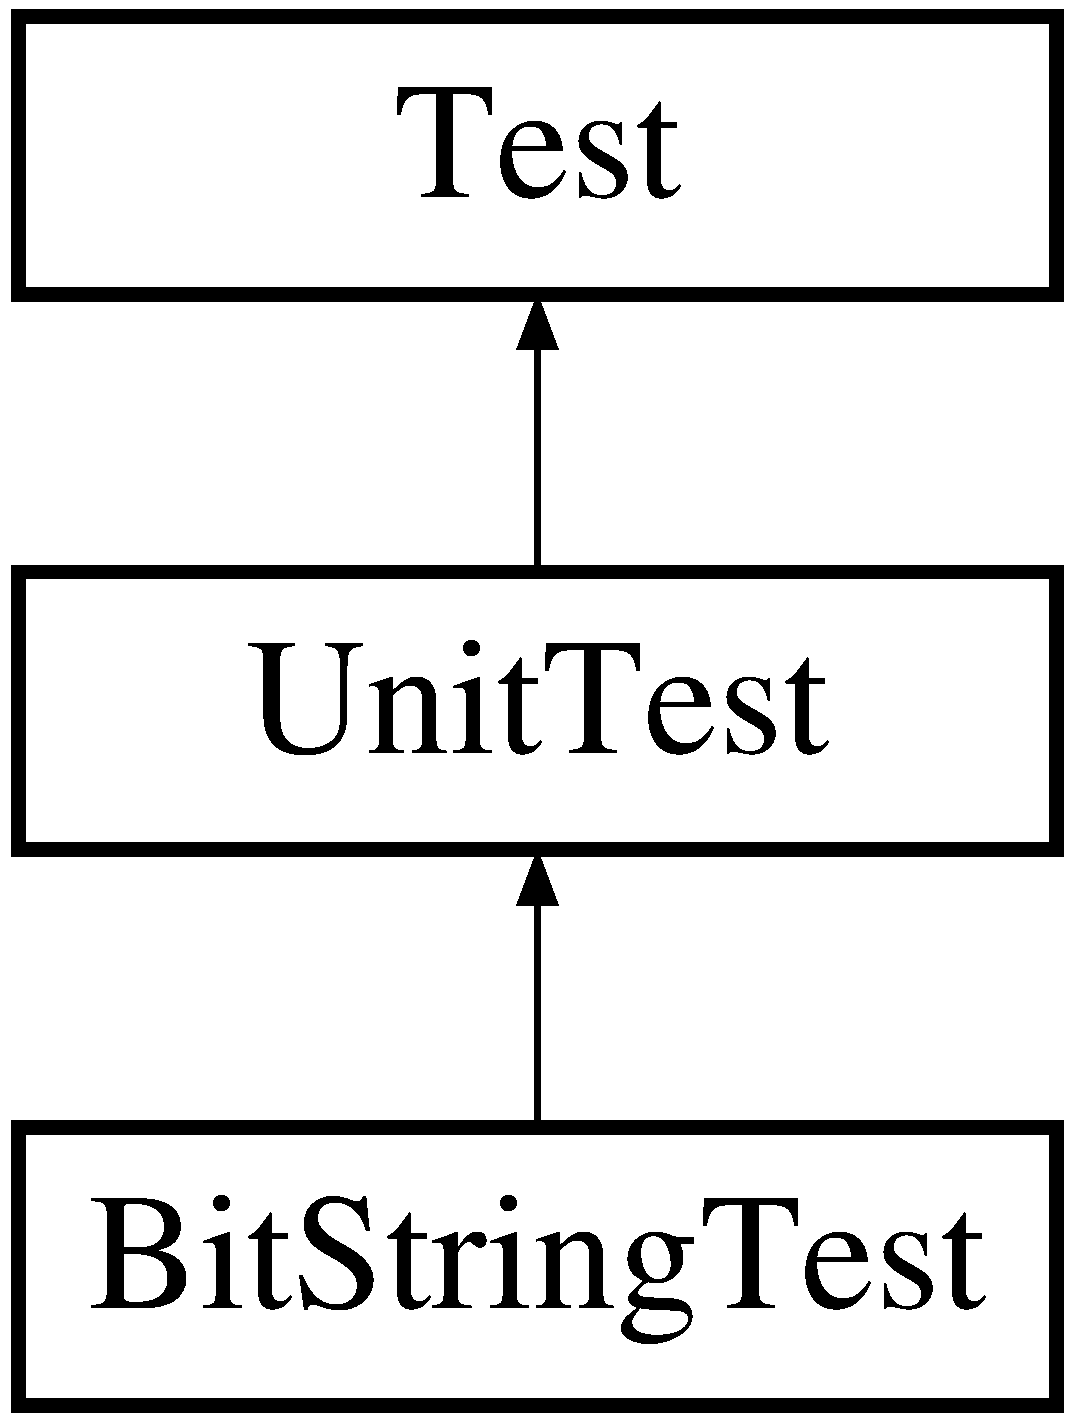
\includegraphics[height=3.000000cm]{classBitStringTest}
\end{center}
\end{figure}
\subsection*{Public Member Functions}
\begin{DoxyCompactItemize}
\item 
\textbf{ Bit\+String\+Test} (\textbf{ Test\+Suite} $\ast$s)
\item 
void \textbf{ setup} (void)
\item 
void \textbf{ cleanup} (void)
\item 
void \textbf{ test\+Bit\+Input\+Output} (void)
\item 
void \textbf{ test\+Length} (void)
\item 
void \textbf{ test\+Datatype\+Input} (void)
\item 
void \textbf{ test\+Datatype\+Output} (void)
\item 
void \textbf{ test\+Equality} (void)
\item 
void \textbf{ test\+Cutting} (void)
\item 
void \textbf{ test\+Compression} (void)
\item 
void \textbf{ test\+Arity} (void)
\end{DoxyCompactItemize}
\subsection*{Private Attributes}
\begin{DoxyCompactItemize}
\item 
\textbf{ Bit\+String} $\ast$ \textbf{ bs\+\_\+0}
\item 
\textbf{ Bit\+String} $\ast$ \textbf{ bs\+\_\+1}
\item 
\textbf{ Bit\+String} $\ast$ \textbf{ bs\+\_\+10}
\item 
\textbf{ Bit\+String} $\ast$ \textbf{ bs\+\_\+001}
\item 
\textbf{ Bit\+String} $\ast$ \textbf{ bs\+\_\+100}
\item 
\textbf{ Bit\+String} $\ast$ \textbf{ bs\+\_\+1010}
\item 
\textbf{ Bit\+String} $\ast$ \textbf{ bs\+\_\+1110}
\item 
\textbf{ Bit\+String} $\ast$ \textbf{ bs\+\_\+01011}
\item 
\textbf{ Bit\+String} $\ast$ \textbf{ bs\+\_\+10010}
\item 
\textbf{ Bit\+String} $\ast$ \textbf{ bs\+\_\+10101110}
\item 
\textbf{ Bit\+String} $\ast$ \textbf{ bs\+\_\+101011101}
\end{DoxyCompactItemize}
\subsection*{Additional Inherited Members}


\subsection{Constructor \& Destructor Documentation}
\mbox{\label{classBitStringTest_a4f00a31731b569f3bdf1e69a48b2db86}} 
\index{Bit\+String\+Test@{Bit\+String\+Test}!Bit\+String\+Test@{Bit\+String\+Test}}
\index{Bit\+String\+Test@{Bit\+String\+Test}!Bit\+String\+Test@{Bit\+String\+Test}}
\subsubsection{Bit\+String\+Test()}
{\footnotesize\ttfamily Bit\+String\+Test\+::\+Bit\+String\+Test (\begin{DoxyParamCaption}\item[{\textbf{ Test\+Suite} $\ast$}]{s }\end{DoxyParamCaption})}



\subsection{Member Function Documentation}
\mbox{\label{classBitStringTest_af7a839ea60ca9e788e480ee74f1ca675}} 
\index{Bit\+String\+Test@{Bit\+String\+Test}!cleanup@{cleanup}}
\index{cleanup@{cleanup}!Bit\+String\+Test@{Bit\+String\+Test}}
\subsubsection{cleanup()}
{\footnotesize\ttfamily void Bit\+String\+Test\+::cleanup (\begin{DoxyParamCaption}\item[{void}]{ }\end{DoxyParamCaption})\hspace{0.3cm}{\ttfamily [virtual]}}

cleanup the unit test -\/ called after run 

Reimplemented from \textbf{ Unit\+Test} \doxyref{}{p.}{classUnitTest_adf77efe972ee4a766d94e3f7ddc193ad}.

\mbox{\label{classBitStringTest_ae3916035aad5f74e4dbcf92be6b4b9a8}} 
\index{Bit\+String\+Test@{Bit\+String\+Test}!setup@{setup}}
\index{setup@{setup}!Bit\+String\+Test@{Bit\+String\+Test}}
\subsubsection{setup()}
{\footnotesize\ttfamily void Bit\+String\+Test\+::setup (\begin{DoxyParamCaption}\item[{void}]{ }\end{DoxyParamCaption})\hspace{0.3cm}{\ttfamily [virtual]}}

setup the unit test -\/ called before run

\doxyref{Unit\+Test\+::setup}{p.}{classUnitTest_ad73fdf9012b651047ea001d21f9d27ad} will (together with \doxyref{Unit\+Test\+::cleanup}{p.}{classUnitTest_adf77efe972ee4a766d94e3f7ddc193ad}) save and restore the object stored in Globs so they should be called from the corresponding functions in the derived object if the derived unit test manipulates the Globs object. 

Reimplemented from \textbf{ Unit\+Test} \doxyref{}{p.}{classUnitTest_ad73fdf9012b651047ea001d21f9d27ad}.

\mbox{\label{classBitStringTest_ae536ce186a0f23634b86f59d0a17e4ce}} 
\index{Bit\+String\+Test@{Bit\+String\+Test}!test\+Arity@{test\+Arity}}
\index{test\+Arity@{test\+Arity}!Bit\+String\+Test@{Bit\+String\+Test}}
\subsubsection{test\+Arity()}
{\footnotesize\ttfamily void Bit\+String\+Test\+::test\+Arity (\begin{DoxyParamCaption}\item[{void}]{ }\end{DoxyParamCaption})}

\mbox{\label{classBitStringTest_a09533dadbf9261c4c39f7f3885814dfa}} 
\index{Bit\+String\+Test@{Bit\+String\+Test}!test\+Bit\+Input\+Output@{test\+Bit\+Input\+Output}}
\index{test\+Bit\+Input\+Output@{test\+Bit\+Input\+Output}!Bit\+String\+Test@{Bit\+String\+Test}}
\subsubsection{test\+Bit\+Input\+Output()}
{\footnotesize\ttfamily void Bit\+String\+Test\+::test\+Bit\+Input\+Output (\begin{DoxyParamCaption}\item[{void}]{ }\end{DoxyParamCaption})}

\mbox{\label{classBitStringTest_aed6caf8441aa111008eefe02bac29cd2}} 
\index{Bit\+String\+Test@{Bit\+String\+Test}!test\+Compression@{test\+Compression}}
\index{test\+Compression@{test\+Compression}!Bit\+String\+Test@{Bit\+String\+Test}}
\subsubsection{test\+Compression()}
{\footnotesize\ttfamily void Bit\+String\+Test\+::test\+Compression (\begin{DoxyParamCaption}\item[{void}]{ }\end{DoxyParamCaption})}

\mbox{\label{classBitStringTest_af4cd832c422c58a9caeba59068840e8f}} 
\index{Bit\+String\+Test@{Bit\+String\+Test}!test\+Cutting@{test\+Cutting}}
\index{test\+Cutting@{test\+Cutting}!Bit\+String\+Test@{Bit\+String\+Test}}
\subsubsection{test\+Cutting()}
{\footnotesize\ttfamily void Bit\+String\+Test\+::test\+Cutting (\begin{DoxyParamCaption}\item[{void}]{ }\end{DoxyParamCaption})}

\mbox{\label{classBitStringTest_a497868d12e5f592ff4efd713711f6a28}} 
\index{Bit\+String\+Test@{Bit\+String\+Test}!test\+Datatype\+Input@{test\+Datatype\+Input}}
\index{test\+Datatype\+Input@{test\+Datatype\+Input}!Bit\+String\+Test@{Bit\+String\+Test}}
\subsubsection{test\+Datatype\+Input()}
{\footnotesize\ttfamily void Bit\+String\+Test\+::test\+Datatype\+Input (\begin{DoxyParamCaption}\item[{void}]{ }\end{DoxyParamCaption})}

\mbox{\label{classBitStringTest_a65e8ff79f1decc35ddbb99ab761854ba}} 
\index{Bit\+String\+Test@{Bit\+String\+Test}!test\+Datatype\+Output@{test\+Datatype\+Output}}
\index{test\+Datatype\+Output@{test\+Datatype\+Output}!Bit\+String\+Test@{Bit\+String\+Test}}
\subsubsection{test\+Datatype\+Output()}
{\footnotesize\ttfamily void Bit\+String\+Test\+::test\+Datatype\+Output (\begin{DoxyParamCaption}\item[{void}]{ }\end{DoxyParamCaption})}

\mbox{\label{classBitStringTest_ab0b15652d7159f9ef41ff262b9864088}} 
\index{Bit\+String\+Test@{Bit\+String\+Test}!test\+Equality@{test\+Equality}}
\index{test\+Equality@{test\+Equality}!Bit\+String\+Test@{Bit\+String\+Test}}
\subsubsection{test\+Equality()}
{\footnotesize\ttfamily void Bit\+String\+Test\+::test\+Equality (\begin{DoxyParamCaption}\item[{void}]{ }\end{DoxyParamCaption})}

\mbox{\label{classBitStringTest_ae56c089336f6a314f10218bbada60718}} 
\index{Bit\+String\+Test@{Bit\+String\+Test}!test\+Length@{test\+Length}}
\index{test\+Length@{test\+Length}!Bit\+String\+Test@{Bit\+String\+Test}}
\subsubsection{test\+Length()}
{\footnotesize\ttfamily void Bit\+String\+Test\+::test\+Length (\begin{DoxyParamCaption}\item[{void}]{ }\end{DoxyParamCaption})}



\subsection{Member Data Documentation}
\mbox{\label{classBitStringTest_a240ecc34787f27a6af863d474da67715}} 
\index{Bit\+String\+Test@{Bit\+String\+Test}!bs\+\_\+0@{bs\+\_\+0}}
\index{bs\+\_\+0@{bs\+\_\+0}!Bit\+String\+Test@{Bit\+String\+Test}}
\subsubsection{bs\+\_\+0}
{\footnotesize\ttfamily \textbf{ Bit\+String}$\ast$ Bit\+String\+Test\+::bs\+\_\+0\hspace{0.3cm}{\ttfamily [private]}}

\mbox{\label{classBitStringTest_abb31362b09119909dcc16b57bf47d0cd}} 
\index{Bit\+String\+Test@{Bit\+String\+Test}!bs\+\_\+001@{bs\+\_\+001}}
\index{bs\+\_\+001@{bs\+\_\+001}!Bit\+String\+Test@{Bit\+String\+Test}}
\subsubsection{bs\+\_\+001}
{\footnotesize\ttfamily \textbf{ Bit\+String} $\ast$ Bit\+String\+Test\+::bs\+\_\+001\hspace{0.3cm}{\ttfamily [private]}}

\mbox{\label{classBitStringTest_aa135e05c946f07a635be5a714a80a27f}} 
\index{Bit\+String\+Test@{Bit\+String\+Test}!bs\+\_\+01011@{bs\+\_\+01011}}
\index{bs\+\_\+01011@{bs\+\_\+01011}!Bit\+String\+Test@{Bit\+String\+Test}}
\subsubsection{bs\+\_\+01011}
{\footnotesize\ttfamily \textbf{ Bit\+String} $\ast$ Bit\+String\+Test\+::bs\+\_\+01011\hspace{0.3cm}{\ttfamily [private]}}

\mbox{\label{classBitStringTest_ade6533bb3aba14ed364367a93d19aa6e}} 
\index{Bit\+String\+Test@{Bit\+String\+Test}!bs\+\_\+1@{bs\+\_\+1}}
\index{bs\+\_\+1@{bs\+\_\+1}!Bit\+String\+Test@{Bit\+String\+Test}}
\subsubsection{bs\+\_\+1}
{\footnotesize\ttfamily \textbf{ Bit\+String} $\ast$ Bit\+String\+Test\+::bs\+\_\+1\hspace{0.3cm}{\ttfamily [private]}}

\mbox{\label{classBitStringTest_a5f623d6a93410cc9337f556a4a36215f}} 
\index{Bit\+String\+Test@{Bit\+String\+Test}!bs\+\_\+10@{bs\+\_\+10}}
\index{bs\+\_\+10@{bs\+\_\+10}!Bit\+String\+Test@{Bit\+String\+Test}}
\subsubsection{bs\+\_\+10}
{\footnotesize\ttfamily \textbf{ Bit\+String} $\ast$ Bit\+String\+Test\+::bs\+\_\+10\hspace{0.3cm}{\ttfamily [private]}}

\mbox{\label{classBitStringTest_a33fc1e49871eecec79b881c002d4b882}} 
\index{Bit\+String\+Test@{Bit\+String\+Test}!bs\+\_\+100@{bs\+\_\+100}}
\index{bs\+\_\+100@{bs\+\_\+100}!Bit\+String\+Test@{Bit\+String\+Test}}
\subsubsection{bs\+\_\+100}
{\footnotesize\ttfamily \textbf{ Bit\+String} $\ast$ Bit\+String\+Test\+::bs\+\_\+100\hspace{0.3cm}{\ttfamily [private]}}

\mbox{\label{classBitStringTest_a4eb3ba5730a51c10bf0a3d375e76fbb1}} 
\index{Bit\+String\+Test@{Bit\+String\+Test}!bs\+\_\+10010@{bs\+\_\+10010}}
\index{bs\+\_\+10010@{bs\+\_\+10010}!Bit\+String\+Test@{Bit\+String\+Test}}
\subsubsection{bs\+\_\+10010}
{\footnotesize\ttfamily \textbf{ Bit\+String} $\ast$ Bit\+String\+Test\+::bs\+\_\+10010\hspace{0.3cm}{\ttfamily [private]}}

\mbox{\label{classBitStringTest_a1f5ff0a2e2fe693442b4877840d8f0f1}} 
\index{Bit\+String\+Test@{Bit\+String\+Test}!bs\+\_\+1010@{bs\+\_\+1010}}
\index{bs\+\_\+1010@{bs\+\_\+1010}!Bit\+String\+Test@{Bit\+String\+Test}}
\subsubsection{bs\+\_\+1010}
{\footnotesize\ttfamily \textbf{ Bit\+String} $\ast$ Bit\+String\+Test\+::bs\+\_\+1010\hspace{0.3cm}{\ttfamily [private]}}

\mbox{\label{classBitStringTest_af5ca8d0718353d2600508067ffba4da5}} 
\index{Bit\+String\+Test@{Bit\+String\+Test}!bs\+\_\+10101110@{bs\+\_\+10101110}}
\index{bs\+\_\+10101110@{bs\+\_\+10101110}!Bit\+String\+Test@{Bit\+String\+Test}}
\subsubsection{bs\+\_\+10101110}
{\footnotesize\ttfamily \textbf{ Bit\+String} $\ast$ Bit\+String\+Test\+::bs\+\_\+10101110\hspace{0.3cm}{\ttfamily [private]}}

\mbox{\label{classBitStringTest_a6ddc43ab7563b7a97c37df98998abf76}} 
\index{Bit\+String\+Test@{Bit\+String\+Test}!bs\+\_\+101011101@{bs\+\_\+101011101}}
\index{bs\+\_\+101011101@{bs\+\_\+101011101}!Bit\+String\+Test@{Bit\+String\+Test}}
\subsubsection{bs\+\_\+101011101}
{\footnotesize\ttfamily \textbf{ Bit\+String} $\ast$ Bit\+String\+Test\+::bs\+\_\+101011101\hspace{0.3cm}{\ttfamily [private]}}

\mbox{\label{classBitStringTest_a48a6b5f97fe87b7b6ca297a48dabe3ef}} 
\index{Bit\+String\+Test@{Bit\+String\+Test}!bs\+\_\+1110@{bs\+\_\+1110}}
\index{bs\+\_\+1110@{bs\+\_\+1110}!Bit\+String\+Test@{Bit\+String\+Test}}
\subsubsection{bs\+\_\+1110}
{\footnotesize\ttfamily \textbf{ Bit\+String} $\ast$ Bit\+String\+Test\+::bs\+\_\+1110\hspace{0.3cm}{\ttfamily [private]}}



The documentation for this class was generated from the following files\+:\begin{DoxyCompactItemize}
\item 
\textbf{ Bit\+String\+Test.\+h}\item 
\textbf{ Bit\+String\+Test.\+cc}\end{DoxyCompactItemize}

\section{Bmp\+File Class Reference}
\label{classBmpFile}\index{Bmp\+File@{Bmp\+File}}


{\ttfamily \#include $<$Bmp\+File.\+h$>$}

Inheritance diagram for Bmp\+File\+:\begin{figure}[H]
\begin{center}
\leavevmode
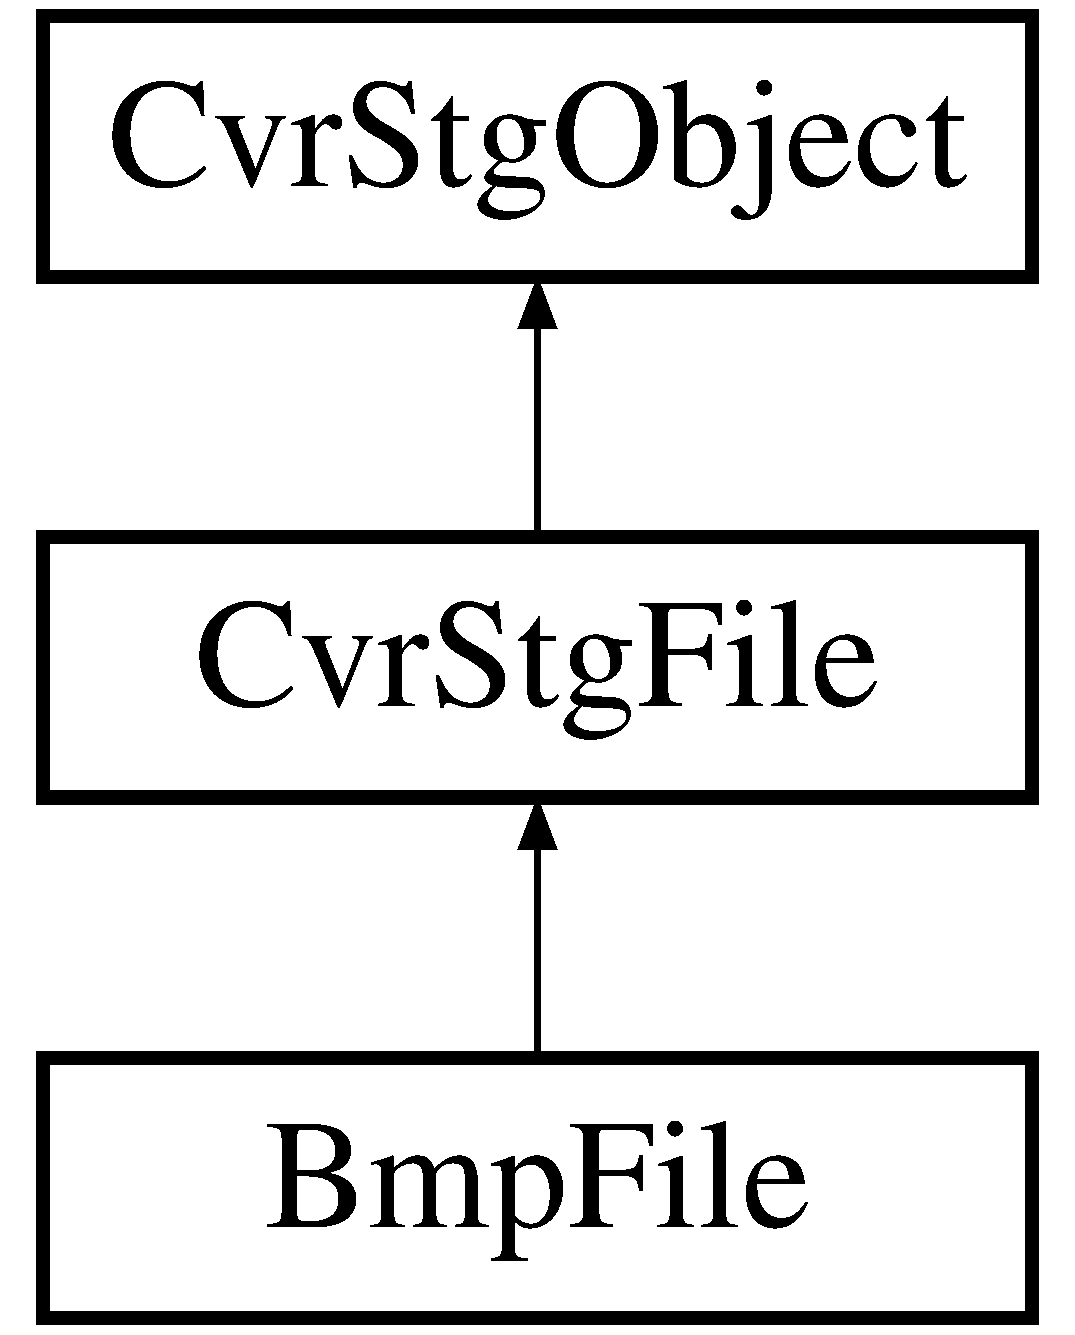
\includegraphics[height=3.000000cm]{classBmpFile}
\end{center}
\end{figure}
\subsection*{Classes}
\begin{DoxyCompactItemize}
\item 
struct \textbf{ struct\+\_\+\+B\+I\+T\+M\+A\+P\+C\+O\+R\+E\+H\+E\+A\+D\+ER}
\item 
struct \textbf{ struct\+\_\+\+B\+I\+T\+M\+A\+P\+F\+I\+L\+E\+H\+E\+A\+D\+ER}
\item 
struct \textbf{ struct\+\_\+\+B\+I\+T\+M\+A\+P\+I\+N\+F\+O\+H\+E\+A\+D\+ER}
\end{DoxyCompactItemize}
\subsection*{Public Member Functions}
\begin{DoxyCompactItemize}
\item 
\textbf{ Bmp\+File} (void)
\item 
\textbf{ Bmp\+File} (\textbf{ Binary\+IO} $\ast$io)
\item 
\textbf{ $\sim$\+Bmp\+File} (void)
\item 
void \textbf{ read} (\textbf{ Binary\+IO} $\ast$io)
\item 
void \textbf{ write} (void)
\item 
std\+::list$<$ \textbf{ Cvr\+Stg\+File\+::\+Property} $>$ \textbf{ get\+Properties} (void) const
\item 
std\+::vector$<$ \textbf{ Matching\+Algorithm} $\ast$ $>$ \textbf{ get\+Matching\+Algorithms} (\textbf{ Graph} $\ast$g, \textbf{ Matching} $\ast$m) const
\item 
unsigned long \textbf{ get\+Num\+Samples} (void) const
\item 
void \textbf{ replace\+Sample} (const \textbf{ Sample\+Pos} pos, const \textbf{ Sample\+Value} $\ast$s)
\item 
\textbf{ Sample\+Value} $\ast$ \textbf{ get\+Sample\+Value} (\textbf{ Sample\+Pos} pos) const
\item 
std\+::vector$<$ \textbf{ Sample\+Value\+Adjacency\+List} $\ast$ $>$ \textbf{ calc\+S\+V\+Adjacency\+Lists} (const std\+::vector$<$ \textbf{ Sample\+Value} $\ast$$>$ \&svs) const
\item 
unsigned short \textbf{ get\+Bit\+Count} (void) const
\item 
unsigned long \textbf{ get\+Width} (void) const
\item 
unsigned long \textbf{ get\+Height} (void) const
\item 
\textbf{ Color\+Palette} $\ast$ \textbf{ get\+Palette} (void) const
\end{DoxyCompactItemize}
\subsection*{Protected Types}
\begin{DoxyCompactItemize}
\item 
typedef struct \textbf{ Bmp\+File\+::struct\+\_\+\+B\+I\+T\+M\+A\+P\+F\+I\+L\+E\+H\+E\+A\+D\+ER} \textbf{ B\+I\+T\+M\+A\+P\+F\+I\+L\+E\+H\+E\+A\+D\+ER}
\item 
typedef struct \textbf{ Bmp\+File\+::struct\+\_\+\+B\+I\+T\+M\+A\+P\+I\+N\+F\+O\+H\+E\+A\+D\+ER} \textbf{ B\+I\+T\+M\+A\+P\+I\+N\+F\+O\+H\+E\+A\+D\+ER}
\item 
typedef struct \textbf{ Bmp\+File\+::struct\+\_\+\+B\+I\+T\+M\+A\+P\+C\+O\+R\+E\+H\+E\+A\+D\+ER} \textbf{ B\+I\+T\+M\+A\+P\+C\+O\+R\+E\+H\+E\+A\+D\+ER}
\end{DoxyCompactItemize}
\subsection*{Private Types}
\begin{DoxyCompactItemize}
\item 
enum \textbf{ S\+U\+B\+F\+O\+R\+M\+AT} \{ \textbf{ W\+IN}, 
\textbf{ O\+S2}
 \}
\end{DoxyCompactItemize}
\subsection*{Private Member Functions}
\begin{DoxyCompactItemize}
\item 
void \textbf{ readheaders} ()
\item 
void \textbf{ bmpwin\+\_\+readheaders} ()
\item 
void \textbf{ bmpos2\+\_\+readheaders} ()
\item 
void \textbf{ writeheaders} ()
\item 
void \textbf{ bmpwin\+\_\+writeheaders} ()
\item 
void \textbf{ bmpos2\+\_\+writeheaders} ()
\item 
void \textbf{ readdata} ()
\item 
void \textbf{ writedata} ()
\item 
void \textbf{ calc\+Index} (\textbf{ Sample\+Pos} pos, unsigned long $\ast$index, unsigned short $\ast$firstbit) const
\item 
unsigned long \textbf{ calc\+Linelength} ()
\item 
\textbf{ S\+U\+B\+F\+O\+R\+M\+AT} \textbf{ get\+Subformat} (void) const
\end{DoxyCompactItemize}
\subsection*{Private Attributes}
\begin{DoxyCompactItemize}
\item 
\textbf{ S\+U\+B\+F\+O\+R\+M\+AT} \textbf{ subformat}
\item 
\textbf{ B\+I\+T\+M\+A\+P\+F\+I\+L\+E\+H\+E\+A\+D\+ER} \textbf{ bmfh}
\item 
\textbf{ B\+I\+T\+M\+A\+P\+I\+N\+F\+O\+H\+E\+A\+D\+ER} \textbf{ bmih}
\item 
\textbf{ B\+I\+T\+M\+A\+P\+C\+O\+R\+E\+H\+E\+A\+D\+ER} \textbf{ bmch}
\item 
\textbf{ Color\+Palette} $\ast$ \textbf{ Palette}
\item 
std\+::vector$<$ std\+::vector$<$ unsigned char $>$ $>$ \textbf{ bitmap}
\item 
std\+::vector$<$ \textbf{ B\+Y\+TE} $>$ \textbf{ Bitmap\+Data}
\item 
std\+::vector$<$ \textbf{ B\+Y\+TE} $>$ \textbf{ atend}
\begin{DoxyCompactList}\small\item\em contains bytes that are appended at the end of the bitmap data (some image editors apparently do this) \end{DoxyCompactList}\end{DoxyCompactItemize}
\subsection*{Static Private Attributes}
\begin{DoxyCompactItemize}
\item 
static const unsigned int \textbf{ Id\+Bm} = 19778
\item 
static const unsigned short \textbf{ Size\+B\+M\+F\+I\+L\+E\+H\+E\+A\+D\+ER} = 14
\item 
static const unsigned short \textbf{ Size\+B\+M\+I\+N\+F\+O\+H\+E\+A\+D\+ER} = 40
\item 
static const unsigned short \textbf{ Size\+B\+M\+C\+O\+R\+E\+H\+E\+A\+D\+ER} = 12
\item 
static const unsigned int \textbf{ C\+O\+M\+P\+R\+E\+S\+S\+I\+O\+N\+\_\+\+B\+I\+\_\+\+R\+GB} = 0
\item 
static const unsigned short \textbf{ Samples\+Per\+Vertex\+\_\+\+Small\+Palette} = 2
\item 
static const unsigned short \textbf{ Samples\+Per\+Vertex\+\_\+\+Large\+Palette} = 3
\item 
static const unsigned short \textbf{ Samples\+Per\+Vertex\+\_\+\+R\+GB} = 2
\item 
static const \textbf{ U\+W\+O\+R\+D32} \textbf{ Radius\+\_\+\+Palette} = 400
\begin{DoxyCompactList}\small\item\em the default radius for palette images (400 = 20$^\wedge$2) \end{DoxyCompactList}\item 
static const \textbf{ U\+W\+O\+R\+D32} \textbf{ Radius\+\_\+\+R\+GB} = 100
\begin{DoxyCompactList}\small\item\em the default radius for R\+GB images (100 = 10$^\wedge$2) \end{DoxyCompactList}\item 
static const \textbf{ Emb\+Value} \textbf{ Emb\+Value\+Modulus\+\_\+\+Small\+Palette} = 2
\item 
static const \textbf{ Emb\+Value} \textbf{ Emb\+Value\+Modulus\+\_\+\+Large\+Palette} = 4
\item 
static const \textbf{ Emb\+Value} \textbf{ Emb\+Value\+Modulus\+\_\+\+R\+GB} = 4
\end{DoxyCompactItemize}
\subsection*{Additional Inherited Members}


\subsection{Member Typedef Documentation}
\mbox{\label{classBmpFile_a897114f7d9b7e66a89f6f3c9eeec4178}} 
\index{Bmp\+File@{Bmp\+File}!B\+I\+T\+M\+A\+P\+C\+O\+R\+E\+H\+E\+A\+D\+ER@{B\+I\+T\+M\+A\+P\+C\+O\+R\+E\+H\+E\+A\+D\+ER}}
\index{B\+I\+T\+M\+A\+P\+C\+O\+R\+E\+H\+E\+A\+D\+ER@{B\+I\+T\+M\+A\+P\+C\+O\+R\+E\+H\+E\+A\+D\+ER}!Bmp\+File@{Bmp\+File}}
\subsubsection{B\+I\+T\+M\+A\+P\+C\+O\+R\+E\+H\+E\+A\+D\+ER}
{\footnotesize\ttfamily typedef struct \textbf{ Bmp\+File\+::struct\+\_\+\+B\+I\+T\+M\+A\+P\+C\+O\+R\+E\+H\+E\+A\+D\+ER}  \textbf{ Bmp\+File\+::\+B\+I\+T\+M\+A\+P\+C\+O\+R\+E\+H\+E\+A\+D\+ER}\hspace{0.3cm}{\ttfamily [protected]}}

\mbox{\label{classBmpFile_a90a9a37736f34d0e1ffb1e8baa6175a5}} 
\index{Bmp\+File@{Bmp\+File}!B\+I\+T\+M\+A\+P\+F\+I\+L\+E\+H\+E\+A\+D\+ER@{B\+I\+T\+M\+A\+P\+F\+I\+L\+E\+H\+E\+A\+D\+ER}}
\index{B\+I\+T\+M\+A\+P\+F\+I\+L\+E\+H\+E\+A\+D\+ER@{B\+I\+T\+M\+A\+P\+F\+I\+L\+E\+H\+E\+A\+D\+ER}!Bmp\+File@{Bmp\+File}}
\subsubsection{B\+I\+T\+M\+A\+P\+F\+I\+L\+E\+H\+E\+A\+D\+ER}
{\footnotesize\ttfamily typedef struct \textbf{ Bmp\+File\+::struct\+\_\+\+B\+I\+T\+M\+A\+P\+F\+I\+L\+E\+H\+E\+A\+D\+ER}  \textbf{ Bmp\+File\+::\+B\+I\+T\+M\+A\+P\+F\+I\+L\+E\+H\+E\+A\+D\+ER}\hspace{0.3cm}{\ttfamily [protected]}}

\mbox{\label{classBmpFile_ae443d9c6b709878f3de3007516530bef}} 
\index{Bmp\+File@{Bmp\+File}!B\+I\+T\+M\+A\+P\+I\+N\+F\+O\+H\+E\+A\+D\+ER@{B\+I\+T\+M\+A\+P\+I\+N\+F\+O\+H\+E\+A\+D\+ER}}
\index{B\+I\+T\+M\+A\+P\+I\+N\+F\+O\+H\+E\+A\+D\+ER@{B\+I\+T\+M\+A\+P\+I\+N\+F\+O\+H\+E\+A\+D\+ER}!Bmp\+File@{Bmp\+File}}
\subsubsection{B\+I\+T\+M\+A\+P\+I\+N\+F\+O\+H\+E\+A\+D\+ER}
{\footnotesize\ttfamily typedef struct \textbf{ Bmp\+File\+::struct\+\_\+\+B\+I\+T\+M\+A\+P\+I\+N\+F\+O\+H\+E\+A\+D\+ER}  \textbf{ Bmp\+File\+::\+B\+I\+T\+M\+A\+P\+I\+N\+F\+O\+H\+E\+A\+D\+ER}\hspace{0.3cm}{\ttfamily [protected]}}



\subsection{Member Enumeration Documentation}
\mbox{\label{classBmpFile_a6404e5c9aa4324ad5aae29db8fc0366c}} 
\index{Bmp\+File@{Bmp\+File}!S\+U\+B\+F\+O\+R\+M\+AT@{S\+U\+B\+F\+O\+R\+M\+AT}}
\index{S\+U\+B\+F\+O\+R\+M\+AT@{S\+U\+B\+F\+O\+R\+M\+AT}!Bmp\+File@{Bmp\+File}}
\subsubsection{S\+U\+B\+F\+O\+R\+M\+AT}
{\footnotesize\ttfamily enum \textbf{ Bmp\+File\+::\+S\+U\+B\+F\+O\+R\+M\+AT}\hspace{0.3cm}{\ttfamily [private]}}

\begin{DoxyEnumFields}{Enumerator}
\raisebox{\heightof{T}}[0pt][0pt]{\index{W\+IN@{W\+IN}!Bmp\+File@{Bmp\+File}}\index{Bmp\+File@{Bmp\+File}!W\+IN@{W\+IN}}}\mbox{\label{classBmpFile_a6404e5c9aa4324ad5aae29db8fc0366ca4debb88cff84bc54592548c435f090e9}} 
W\+IN&\\
\hline

\raisebox{\heightof{T}}[0pt][0pt]{\index{O\+S2@{O\+S2}!Bmp\+File@{Bmp\+File}}\index{Bmp\+File@{Bmp\+File}!O\+S2@{O\+S2}}}\mbox{\label{classBmpFile_a6404e5c9aa4324ad5aae29db8fc0366ca3ea20d80509d0444e5cc4fca76883ef9}} 
O\+S2&\\
\hline

\end{DoxyEnumFields}


\subsection{Constructor \& Destructor Documentation}
\mbox{\label{classBmpFile_a59bd454558c8592e5895a215bbfb3e5c}} 
\index{Bmp\+File@{Bmp\+File}!Bmp\+File@{Bmp\+File}}
\index{Bmp\+File@{Bmp\+File}!Bmp\+File@{Bmp\+File}}
\subsubsection{Bmp\+File()\hspace{0.1cm}{\footnotesize\ttfamily [1/2]}}
{\footnotesize\ttfamily Bmp\+File\+::\+Bmp\+File (\begin{DoxyParamCaption}\item[{void}]{ }\end{DoxyParamCaption})}

\mbox{\label{classBmpFile_a7008eb6ae2f402dd81d2e41175d015a8}} 
\index{Bmp\+File@{Bmp\+File}!Bmp\+File@{Bmp\+File}}
\index{Bmp\+File@{Bmp\+File}!Bmp\+File@{Bmp\+File}}
\subsubsection{Bmp\+File()\hspace{0.1cm}{\footnotesize\ttfamily [2/2]}}
{\footnotesize\ttfamily Bmp\+File\+::\+Bmp\+File (\begin{DoxyParamCaption}\item[{\textbf{ Binary\+IO} $\ast$}]{io }\end{DoxyParamCaption})}

\mbox{\label{classBmpFile_abae6dcc47a03f181d442eb39c79736a3}} 
\index{Bmp\+File@{Bmp\+File}!````~Bmp\+File@{$\sim$\+Bmp\+File}}
\index{````~Bmp\+File@{$\sim$\+Bmp\+File}!Bmp\+File@{Bmp\+File}}
\subsubsection{$\sim$\+Bmp\+File()}
{\footnotesize\ttfamily Bmp\+File\+::$\sim$\+Bmp\+File (\begin{DoxyParamCaption}\item[{void}]{ }\end{DoxyParamCaption})}



\subsection{Member Function Documentation}
\mbox{\label{classBmpFile_a3ae3e9093381579260981ce8857a445d}} 
\index{Bmp\+File@{Bmp\+File}!bmpos2\+\_\+readheaders@{bmpos2\+\_\+readheaders}}
\index{bmpos2\+\_\+readheaders@{bmpos2\+\_\+readheaders}!Bmp\+File@{Bmp\+File}}
\subsubsection{bmpos2\+\_\+readheaders()}
{\footnotesize\ttfamily void Bmp\+File\+::bmpos2\+\_\+readheaders (\begin{DoxyParamCaption}{ }\end{DoxyParamCaption})\hspace{0.3cm}{\ttfamily [private]}}

\mbox{\label{classBmpFile_a3ab6ae9948e2c83669ce86a1b4a99edb}} 
\index{Bmp\+File@{Bmp\+File}!bmpos2\+\_\+writeheaders@{bmpos2\+\_\+writeheaders}}
\index{bmpos2\+\_\+writeheaders@{bmpos2\+\_\+writeheaders}!Bmp\+File@{Bmp\+File}}
\subsubsection{bmpos2\+\_\+writeheaders()}
{\footnotesize\ttfamily void Bmp\+File\+::bmpos2\+\_\+writeheaders (\begin{DoxyParamCaption}{ }\end{DoxyParamCaption})\hspace{0.3cm}{\ttfamily [private]}}

\mbox{\label{classBmpFile_abc31e0f4cc20d7e1243a012e3bf8988f}} 
\index{Bmp\+File@{Bmp\+File}!bmpwin\+\_\+readheaders@{bmpwin\+\_\+readheaders}}
\index{bmpwin\+\_\+readheaders@{bmpwin\+\_\+readheaders}!Bmp\+File@{Bmp\+File}}
\subsubsection{bmpwin\+\_\+readheaders()}
{\footnotesize\ttfamily void Bmp\+File\+::bmpwin\+\_\+readheaders (\begin{DoxyParamCaption}{ }\end{DoxyParamCaption})\hspace{0.3cm}{\ttfamily [private]}}

\mbox{\label{classBmpFile_ae59dc89212474f3b43a537073b80f060}} 
\index{Bmp\+File@{Bmp\+File}!bmpwin\+\_\+writeheaders@{bmpwin\+\_\+writeheaders}}
\index{bmpwin\+\_\+writeheaders@{bmpwin\+\_\+writeheaders}!Bmp\+File@{Bmp\+File}}
\subsubsection{bmpwin\+\_\+writeheaders()}
{\footnotesize\ttfamily void Bmp\+File\+::bmpwin\+\_\+writeheaders (\begin{DoxyParamCaption}{ }\end{DoxyParamCaption})\hspace{0.3cm}{\ttfamily [private]}}

\mbox{\label{classBmpFile_af1f3faff36705b9b496ebc50bf5aa691}} 
\index{Bmp\+File@{Bmp\+File}!calc\+Index@{calc\+Index}}
\index{calc\+Index@{calc\+Index}!Bmp\+File@{Bmp\+File}}
\subsubsection{calc\+Index()}
{\footnotesize\ttfamily void Bmp\+File\+::calc\+Index (\begin{DoxyParamCaption}\item[{\textbf{ Sample\+Pos}}]{pos,  }\item[{unsigned long $\ast$}]{index,  }\item[{unsigned short $\ast$}]{firstbit }\end{DoxyParamCaption}) const\hspace{0.3cm}{\ttfamily [private]}}

translate a sample position into a $<$index,firstbit$>$ pair \char`\"{}pointing\char`\"{} into the Bitmap\+Data array 
\begin{DoxyParams}{Parameters}
{\em pos} & a sample position \\
\hline
{\em index} & a pointer to a variable that will contain the array index used to access the pos-\/th sample \\
\hline
{\em firstbit} & the firstbit in Bitmap\+Data[index] that belongs to the sample with the given position \\
\hline
\end{DoxyParams}
\mbox{\label{classBmpFile_ac102e4126e23158629e174f757374b26}} 
\index{Bmp\+File@{Bmp\+File}!calc\+Linelength@{calc\+Linelength}}
\index{calc\+Linelength@{calc\+Linelength}!Bmp\+File@{Bmp\+File}}
\subsubsection{calc\+Linelength()}
{\footnotesize\ttfamily unsigned long Bmp\+File\+::calc\+Linelength (\begin{DoxyParamCaption}{ }\end{DoxyParamCaption})\hspace{0.3cm}{\ttfamily [private]}}

\mbox{\label{classBmpFile_a4a4e207e07864d6f862bb3bfb5f9cd12}} 
\index{Bmp\+File@{Bmp\+File}!calc\+S\+V\+Adjacency\+Lists@{calc\+S\+V\+Adjacency\+Lists}}
\index{calc\+S\+V\+Adjacency\+Lists@{calc\+S\+V\+Adjacency\+Lists}!Bmp\+File@{Bmp\+File}}
\subsubsection{calc\+S\+V\+Adjacency\+Lists()}
{\footnotesize\ttfamily std\+::vector$<$ \textbf{ Sample\+Value\+Adjacency\+List} $\ast$ $>$ Bmp\+File\+::calc\+S\+V\+Adjacency\+Lists (\begin{DoxyParamCaption}\item[{const std\+::vector$<$ \textbf{ Sample\+Value} $\ast$$>$ \&}]{svs }\end{DoxyParamCaption}) const\hspace{0.3cm}{\ttfamily [virtual]}}

calculate a vector a Sample\+Value\+Adjacency\+Lists 
\begin{DoxyParams}{Parameters}
{\em svs} & a vector of unique(!) sample values where svs[i]-\/$>$get\+Label() == i holds for all i \\
\hline
\end{DoxyParams}
\begin{DoxyReturn}{Returns}
a vector of Sample\+Value\+Adjacency\+Lists where retval[i] only contains sample values with get\+Emb\+Value() == i
\end{DoxyReturn}
Every row in the adjacency lists must be sorted in the following order\+: The first sample value has the least distance to the source sample value, the last has the largest distance. If two sample values in one row have the same distance to the source sample value, the order does not matter.

May be overridden in derived class to provide a faster version. 

Reimplemented from \textbf{ Cvr\+Stg\+File} \doxyref{}{p.}{classCvrStgFile_a5969e7a6a948067673a977b4c539d354}.

\mbox{\label{classBmpFile_ad23c28df703b051f34fc1b052176aa31}} 
\index{Bmp\+File@{Bmp\+File}!get\+Bit\+Count@{get\+Bit\+Count}}
\index{get\+Bit\+Count@{get\+Bit\+Count}!Bmp\+File@{Bmp\+File}}
\subsubsection{get\+Bit\+Count()}
{\footnotesize\ttfamily unsigned short Bmp\+File\+::get\+Bit\+Count (\begin{DoxyParamCaption}\item[{void}]{ }\end{DoxyParamCaption}) const}

\mbox{\label{classBmpFile_ad7016b6b79ba7ec67e569f86fd237c52}} 
\index{Bmp\+File@{Bmp\+File}!get\+Height@{get\+Height}}
\index{get\+Height@{get\+Height}!Bmp\+File@{Bmp\+File}}
\subsubsection{get\+Height()}
{\footnotesize\ttfamily unsigned long Bmp\+File\+::get\+Height (\begin{DoxyParamCaption}\item[{void}]{ }\end{DoxyParamCaption}) const}

\mbox{\label{classBmpFile_ab9dedf8aeebeaa832bb290991f94fc89}} 
\index{Bmp\+File@{Bmp\+File}!get\+Matching\+Algorithms@{get\+Matching\+Algorithms}}
\index{get\+Matching\+Algorithms@{get\+Matching\+Algorithms}!Bmp\+File@{Bmp\+File}}
\subsubsection{get\+Matching\+Algorithms()}
{\footnotesize\ttfamily std\+::vector$<$ \textbf{ Matching\+Algorithm} $\ast$ $>$ Bmp\+File\+::get\+Matching\+Algorithms (\begin{DoxyParamCaption}\item[{\textbf{ Graph} $\ast$}]{g,  }\item[{\textbf{ Matching} $\ast$}]{m }\end{DoxyParamCaption}) const\hspace{0.3cm}{\ttfamily [virtual]}}

get recommended list of matching algorithms 
\begin{DoxyParams}{Parameters}
{\em m} & an empty matching -\/ will be used in construction of \doxyref{Matching\+Algorithm}{p.}{classMatchingAlgorithm} objects\\
\hline
\end{DoxyParams}
The \doxyref{Matching\+Algorithm}{p.}{classMatchingAlgorithm} objects returned by this function should be deleted by the caller if they are no longer needed. 

Reimplemented from \textbf{ Cvr\+Stg\+File} \doxyref{}{p.}{classCvrStgFile_aa0b1087f94e191b72e794a56e49bb706}.

\mbox{\label{classBmpFile_a564fb90235f06c80162b9086dcc6e78d}} 
\index{Bmp\+File@{Bmp\+File}!get\+Num\+Samples@{get\+Num\+Samples}}
\index{get\+Num\+Samples@{get\+Num\+Samples}!Bmp\+File@{Bmp\+File}}
\subsubsection{get\+Num\+Samples()}
{\footnotesize\ttfamily unsigned long Bmp\+File\+::get\+Num\+Samples (\begin{DoxyParamCaption}\item[{void}]{ }\end{DoxyParamCaption}) const\hspace{0.3cm}{\ttfamily [virtual]}}

get the number of samples in this \doxyref{Cvr\+Stg\+Object}{p.}{classCvrStgObject} 

Implements \textbf{ Cvr\+Stg\+Object} \doxyref{}{p.}{classCvrStgObject_a80ae8f095b66683e5207adf8ff8265b4}.

\mbox{\label{classBmpFile_a95e71e37b6e9752527d438623a924c7a}} 
\index{Bmp\+File@{Bmp\+File}!get\+Palette@{get\+Palette}}
\index{get\+Palette@{get\+Palette}!Bmp\+File@{Bmp\+File}}
\subsubsection{get\+Palette()}
{\footnotesize\ttfamily \textbf{ Color\+Palette} $\ast$ Bmp\+File\+::get\+Palette (\begin{DoxyParamCaption}\item[{void}]{ }\end{DoxyParamCaption}) const}

\mbox{\label{classBmpFile_acc609c77bb5fdc4260bd40f76e7286e6}} 
\index{Bmp\+File@{Bmp\+File}!get\+Properties@{get\+Properties}}
\index{get\+Properties@{get\+Properties}!Bmp\+File@{Bmp\+File}}
\subsubsection{get\+Properties()}
{\footnotesize\ttfamily std\+::list$<$ \textbf{ Cvr\+Stg\+File\+::\+Property} $>$ Bmp\+File\+::get\+Properties (\begin{DoxyParamCaption}\item[{void}]{ }\end{DoxyParamCaption}) const\hspace{0.3cm}{\ttfamily [virtual]}}



Implements \textbf{ Cvr\+Stg\+File} \doxyref{}{p.}{classCvrStgFile_afe2f570ea6447c0636093b44ff7793cc}.

\mbox{\label{classBmpFile_a8a982a74d9d5ef1a33228859e51c888b}} 
\index{Bmp\+File@{Bmp\+File}!get\+Sample\+Value@{get\+Sample\+Value}}
\index{get\+Sample\+Value@{get\+Sample\+Value}!Bmp\+File@{Bmp\+File}}
\subsubsection{get\+Sample\+Value()}
{\footnotesize\ttfamily \textbf{ Sample\+Value} $\ast$ Bmp\+File\+::get\+Sample\+Value (\begin{DoxyParamCaption}\item[{\textbf{ Sample\+Pos}}]{pos }\end{DoxyParamCaption}) const\hspace{0.3cm}{\ttfamily [virtual]}}

get the sample at position pos 
\begin{DoxyParams}{Parameters}
{\em pos} & the position of a sample (must be in 0...\doxyref{get\+Num\+Samples()}{p.}{classBmpFile_a564fb90235f06c80162b9086dcc6e78d}-\/1) \\
\hline
\end{DoxyParams}
\begin{DoxyReturn}{Returns}
the sample at the given position
\end{DoxyReturn}
The sample object is created in this function and should be deleted by the caller. The derived class should check the condition(s) given above in its Implementation of this function. 

Implements \textbf{ Cvr\+Stg\+Object} \doxyref{}{p.}{classCvrStgObject_ac77a8da85a4f7b53e2166e990dfaa4f2}.

\mbox{\label{classBmpFile_aa49be0847a8e260564f5996d75fc5326}} 
\index{Bmp\+File@{Bmp\+File}!get\+Subformat@{get\+Subformat}}
\index{get\+Subformat@{get\+Subformat}!Bmp\+File@{Bmp\+File}}
\subsubsection{get\+Subformat()}
{\footnotesize\ttfamily \textbf{ Bmp\+File\+::\+S\+U\+B\+F\+O\+R\+M\+AT} Bmp\+File\+::get\+Subformat (\begin{DoxyParamCaption}\item[{void}]{ }\end{DoxyParamCaption}) const\hspace{0.3cm}{\ttfamily [private]}}

\mbox{\label{classBmpFile_a9e4cd6a539139ddeedc5a23079c72663}} 
\index{Bmp\+File@{Bmp\+File}!get\+Width@{get\+Width}}
\index{get\+Width@{get\+Width}!Bmp\+File@{Bmp\+File}}
\subsubsection{get\+Width()}
{\footnotesize\ttfamily unsigned long Bmp\+File\+::get\+Width (\begin{DoxyParamCaption}\item[{void}]{ }\end{DoxyParamCaption}) const}

\mbox{\label{classBmpFile_a626da8e445ba96fb6372cc2769ef5cfd}} 
\index{Bmp\+File@{Bmp\+File}!read@{read}}
\index{read@{read}!Bmp\+File@{Bmp\+File}}
\subsubsection{read()}
{\footnotesize\ttfamily void Bmp\+File\+::read (\begin{DoxyParamCaption}\item[{\textbf{ Binary\+IO} $\ast$}]{io }\end{DoxyParamCaption})\hspace{0.3cm}{\ttfamily [virtual]}}



Reimplemented from \textbf{ Cvr\+Stg\+File} \doxyref{}{p.}{classCvrStgFile_a8a568ccb2ad5d6c178f764dca6090908}.

\mbox{\label{classBmpFile_ab9a22d02a32a6901c8b3c4fbaa2d37ed}} 
\index{Bmp\+File@{Bmp\+File}!readdata@{readdata}}
\index{readdata@{readdata}!Bmp\+File@{Bmp\+File}}
\subsubsection{readdata()}
{\footnotesize\ttfamily void Bmp\+File\+::readdata (\begin{DoxyParamCaption}{ }\end{DoxyParamCaption})\hspace{0.3cm}{\ttfamily [private]}}

\mbox{\label{classBmpFile_af91c186f49fdb8b1056934fff598c1a0}} 
\index{Bmp\+File@{Bmp\+File}!readheaders@{readheaders}}
\index{readheaders@{readheaders}!Bmp\+File@{Bmp\+File}}
\subsubsection{readheaders()}
{\footnotesize\ttfamily void Bmp\+File\+::readheaders (\begin{DoxyParamCaption}{ }\end{DoxyParamCaption})\hspace{0.3cm}{\ttfamily [private]}}

\mbox{\label{classBmpFile_a9f476c72483674452cf272f9e10d1087}} 
\index{Bmp\+File@{Bmp\+File}!replace\+Sample@{replace\+Sample}}
\index{replace\+Sample@{replace\+Sample}!Bmp\+File@{Bmp\+File}}
\subsubsection{replace\+Sample()}
{\footnotesize\ttfamily void Bmp\+File\+::replace\+Sample (\begin{DoxyParamCaption}\item[{const \textbf{ Sample\+Pos}}]{pos,  }\item[{const \textbf{ Sample\+Value} $\ast$}]{s }\end{DoxyParamCaption})\hspace{0.3cm}{\ttfamily [virtual]}}

replace a sample thus (possibly) altering the value of the bit returned by Sample\+Value-\/$>$get\+Bit() 
\begin{DoxyParams}{Parameters}
{\em pos} & the position of the sample (must be in 0...\doxyref{get\+Num\+Samples()}{p.}{classBmpFile_a564fb90235f06c80162b9086dcc6e78d}-\/1) \\
\hline
{\em s} & the sample value that should replace the current sample value (must be of correct type for this \doxyref{Cvr\+Stg\+Object}{p.}{classCvrStgObject})\\
\hline
\end{DoxyParams}
The derived class should check the condition(s) given above in its Implementation of this function. 

Implements \textbf{ Cvr\+Stg\+Object} \doxyref{}{p.}{classCvrStgObject_a3068d6a9dcc1c0b8bde2f081cfde6ce5}.

\mbox{\label{classBmpFile_ad1ab3f4964c187a0d2c23f14f9a278af}} 
\index{Bmp\+File@{Bmp\+File}!write@{write}}
\index{write@{write}!Bmp\+File@{Bmp\+File}}
\subsubsection{write()}
{\footnotesize\ttfamily void Bmp\+File\+::write (\begin{DoxyParamCaption}\item[{void}]{ }\end{DoxyParamCaption})\hspace{0.3cm}{\ttfamily [virtual]}}



Reimplemented from \textbf{ Cvr\+Stg\+File} \doxyref{}{p.}{classCvrStgFile_af2b8f47f83f9210409af6be7d750a841}.

\mbox{\label{classBmpFile_a3b433fac7315fdc42c50e58a2c65eef7}} 
\index{Bmp\+File@{Bmp\+File}!writedata@{writedata}}
\index{writedata@{writedata}!Bmp\+File@{Bmp\+File}}
\subsubsection{writedata()}
{\footnotesize\ttfamily void Bmp\+File\+::writedata (\begin{DoxyParamCaption}{ }\end{DoxyParamCaption})\hspace{0.3cm}{\ttfamily [private]}}

\mbox{\label{classBmpFile_a5912cb13cc1bb1f837671d61950ed219}} 
\index{Bmp\+File@{Bmp\+File}!writeheaders@{writeheaders}}
\index{writeheaders@{writeheaders}!Bmp\+File@{Bmp\+File}}
\subsubsection{writeheaders()}
{\footnotesize\ttfamily void Bmp\+File\+::writeheaders (\begin{DoxyParamCaption}{ }\end{DoxyParamCaption})\hspace{0.3cm}{\ttfamily [private]}}



\subsection{Member Data Documentation}
\mbox{\label{classBmpFile_a9e65f30114e66be87fb7110e2328d2c3}} 
\index{Bmp\+File@{Bmp\+File}!atend@{atend}}
\index{atend@{atend}!Bmp\+File@{Bmp\+File}}
\subsubsection{atend}
{\footnotesize\ttfamily std\+::vector$<$\textbf{ B\+Y\+TE}$>$ Bmp\+File\+::atend\hspace{0.3cm}{\ttfamily [private]}}

\mbox{\label{classBmpFile_a9f0a6ff821e71cf2aaf4965a1a53eb4e}} 
\index{Bmp\+File@{Bmp\+File}!bitmap@{bitmap}}
\index{bitmap@{bitmap}!Bmp\+File@{Bmp\+File}}
\subsubsection{bitmap}
{\footnotesize\ttfamily std\+::vector$<$std\+::vector $<$unsigned char$>$ $>$ Bmp\+File\+::bitmap\hspace{0.3cm}{\ttfamily [private]}}

contains the bitmap in the following format bitmap[i] is the pixel data of the i-\/th row of the bitmap bitmap[i][j] is the j-\/th byte of the pixel data of the i-\/th row of the bitmap if bitcount is $<$ 8 then bitmap[i][j] contains the pixels as read in from the file (i.\+e. in the \char`\"{}wrong\char`\"{} direction) this is taken care of in the calc\+R\+CB function \mbox{\label{classBmpFile_aa9246cb941c51d2e5609dd322c9b684a}} 
\index{Bmp\+File@{Bmp\+File}!Bitmap\+Data@{Bitmap\+Data}}
\index{Bitmap\+Data@{Bitmap\+Data}!Bmp\+File@{Bmp\+File}}
\subsubsection{Bitmap\+Data}
{\footnotesize\ttfamily std\+::vector$<$\textbf{ B\+Y\+TE}$>$ Bmp\+File\+::\+Bitmap\+Data\hspace{0.3cm}{\ttfamily [private]}}

contains the bitmap data in the same order as read from file (but without padding bytes) \mbox{\label{classBmpFile_aaca86a5389fc68c40cdf30b37acf3d94}} 
\index{Bmp\+File@{Bmp\+File}!bmch@{bmch}}
\index{bmch@{bmch}!Bmp\+File@{Bmp\+File}}
\subsubsection{bmch}
{\footnotesize\ttfamily \textbf{ B\+I\+T\+M\+A\+P\+C\+O\+R\+E\+H\+E\+A\+D\+ER} Bmp\+File\+::bmch\hspace{0.3cm}{\ttfamily [private]}}

\mbox{\label{classBmpFile_ab6e68a5be1e5d2c9fb96c8a6bb167c41}} 
\index{Bmp\+File@{Bmp\+File}!bmfh@{bmfh}}
\index{bmfh@{bmfh}!Bmp\+File@{Bmp\+File}}
\subsubsection{bmfh}
{\footnotesize\ttfamily \textbf{ B\+I\+T\+M\+A\+P\+F\+I\+L\+E\+H\+E\+A\+D\+ER} Bmp\+File\+::bmfh\hspace{0.3cm}{\ttfamily [private]}}

\mbox{\label{classBmpFile_a1aa4569052f459f3e99d290120b9dd94}} 
\index{Bmp\+File@{Bmp\+File}!bmih@{bmih}}
\index{bmih@{bmih}!Bmp\+File@{Bmp\+File}}
\subsubsection{bmih}
{\footnotesize\ttfamily \textbf{ B\+I\+T\+M\+A\+P\+I\+N\+F\+O\+H\+E\+A\+D\+ER} Bmp\+File\+::bmih\hspace{0.3cm}{\ttfamily [private]}}

\mbox{\label{classBmpFile_a7fb79389dda23b0526b76bee5e61c320}} 
\index{Bmp\+File@{Bmp\+File}!C\+O\+M\+P\+R\+E\+S\+S\+I\+O\+N\+\_\+\+B\+I\+\_\+\+R\+GB@{C\+O\+M\+P\+R\+E\+S\+S\+I\+O\+N\+\_\+\+B\+I\+\_\+\+R\+GB}}
\index{C\+O\+M\+P\+R\+E\+S\+S\+I\+O\+N\+\_\+\+B\+I\+\_\+\+R\+GB@{C\+O\+M\+P\+R\+E\+S\+S\+I\+O\+N\+\_\+\+B\+I\+\_\+\+R\+GB}!Bmp\+File@{Bmp\+File}}
\subsubsection{C\+O\+M\+P\+R\+E\+S\+S\+I\+O\+N\+\_\+\+B\+I\+\_\+\+R\+GB}
{\footnotesize\ttfamily const unsigned int Bmp\+File\+::\+C\+O\+M\+P\+R\+E\+S\+S\+I\+O\+N\+\_\+\+B\+I\+\_\+\+R\+GB = 0\hspace{0.3cm}{\ttfamily [static]}, {\ttfamily [private]}}

\mbox{\label{classBmpFile_a6c674aec59a1e5a1b8f6481e54a147ac}} 
\index{Bmp\+File@{Bmp\+File}!Emb\+Value\+Modulus\+\_\+\+Large\+Palette@{Emb\+Value\+Modulus\+\_\+\+Large\+Palette}}
\index{Emb\+Value\+Modulus\+\_\+\+Large\+Palette@{Emb\+Value\+Modulus\+\_\+\+Large\+Palette}!Bmp\+File@{Bmp\+File}}
\subsubsection{Emb\+Value\+Modulus\+\_\+\+Large\+Palette}
{\footnotesize\ttfamily const \textbf{ Emb\+Value} Bmp\+File\+::\+Emb\+Value\+Modulus\+\_\+\+Large\+Palette = 4\hspace{0.3cm}{\ttfamily [static]}, {\ttfamily [private]}}

\mbox{\label{classBmpFile_a32fc1b03aba7a94b7523addff3c007d8}} 
\index{Bmp\+File@{Bmp\+File}!Emb\+Value\+Modulus\+\_\+\+R\+GB@{Emb\+Value\+Modulus\+\_\+\+R\+GB}}
\index{Emb\+Value\+Modulus\+\_\+\+R\+GB@{Emb\+Value\+Modulus\+\_\+\+R\+GB}!Bmp\+File@{Bmp\+File}}
\subsubsection{Emb\+Value\+Modulus\+\_\+\+R\+GB}
{\footnotesize\ttfamily const \textbf{ Emb\+Value} Bmp\+File\+::\+Emb\+Value\+Modulus\+\_\+\+R\+GB = 4\hspace{0.3cm}{\ttfamily [static]}, {\ttfamily [private]}}

\mbox{\label{classBmpFile_a8823c9e4c01d1d950540e3dc17835d20}} 
\index{Bmp\+File@{Bmp\+File}!Emb\+Value\+Modulus\+\_\+\+Small\+Palette@{Emb\+Value\+Modulus\+\_\+\+Small\+Palette}}
\index{Emb\+Value\+Modulus\+\_\+\+Small\+Palette@{Emb\+Value\+Modulus\+\_\+\+Small\+Palette}!Bmp\+File@{Bmp\+File}}
\subsubsection{Emb\+Value\+Modulus\+\_\+\+Small\+Palette}
{\footnotesize\ttfamily const \textbf{ Emb\+Value} Bmp\+File\+::\+Emb\+Value\+Modulus\+\_\+\+Small\+Palette = 2\hspace{0.3cm}{\ttfamily [static]}, {\ttfamily [private]}}

\mbox{\label{classBmpFile_aeec5116ac502e161779825827e6f59e0}} 
\index{Bmp\+File@{Bmp\+File}!Id\+Bm@{Id\+Bm}}
\index{Id\+Bm@{Id\+Bm}!Bmp\+File@{Bmp\+File}}
\subsubsection{Id\+Bm}
{\footnotesize\ttfamily const unsigned int Bmp\+File\+::\+Id\+Bm = 19778\hspace{0.3cm}{\ttfamily [static]}, {\ttfamily [private]}}

\mbox{\label{classBmpFile_a6c56c60fcfa09a9e937311d40e86f7fe}} 
\index{Bmp\+File@{Bmp\+File}!Palette@{Palette}}
\index{Palette@{Palette}!Bmp\+File@{Bmp\+File}}
\subsubsection{Palette}
{\footnotesize\ttfamily \textbf{ Color\+Palette}$\ast$ Bmp\+File\+::\+Palette\hspace{0.3cm}{\ttfamily [private]}}

\mbox{\label{classBmpFile_a67e3867c388c9e68516a7c76b8c65b8d}} 
\index{Bmp\+File@{Bmp\+File}!Radius\+\_\+\+Palette@{Radius\+\_\+\+Palette}}
\index{Radius\+\_\+\+Palette@{Radius\+\_\+\+Palette}!Bmp\+File@{Bmp\+File}}
\subsubsection{Radius\+\_\+\+Palette}
{\footnotesize\ttfamily const \textbf{ U\+W\+O\+R\+D32} Bmp\+File\+::\+Radius\+\_\+\+Palette = 400\hspace{0.3cm}{\ttfamily [static]}, {\ttfamily [private]}}

\mbox{\label{classBmpFile_a1acbeb684e15579bea2e18d74d65f37e}} 
\index{Bmp\+File@{Bmp\+File}!Radius\+\_\+\+R\+GB@{Radius\+\_\+\+R\+GB}}
\index{Radius\+\_\+\+R\+GB@{Radius\+\_\+\+R\+GB}!Bmp\+File@{Bmp\+File}}
\subsubsection{Radius\+\_\+\+R\+GB}
{\footnotesize\ttfamily const \textbf{ U\+W\+O\+R\+D32} Bmp\+File\+::\+Radius\+\_\+\+R\+GB = 100\hspace{0.3cm}{\ttfamily [static]}, {\ttfamily [private]}}

\mbox{\label{classBmpFile_aab7eda4b026a70aaeec2d0946ad54c52}} 
\index{Bmp\+File@{Bmp\+File}!Samples\+Per\+Vertex\+\_\+\+Large\+Palette@{Samples\+Per\+Vertex\+\_\+\+Large\+Palette}}
\index{Samples\+Per\+Vertex\+\_\+\+Large\+Palette@{Samples\+Per\+Vertex\+\_\+\+Large\+Palette}!Bmp\+File@{Bmp\+File}}
\subsubsection{Samples\+Per\+Vertex\+\_\+\+Large\+Palette}
{\footnotesize\ttfamily const unsigned short Bmp\+File\+::\+Samples\+Per\+Vertex\+\_\+\+Large\+Palette = 3\hspace{0.3cm}{\ttfamily [static]}, {\ttfamily [private]}}

\mbox{\label{classBmpFile_aee8003b8bd509706205423a44a607de9}} 
\index{Bmp\+File@{Bmp\+File}!Samples\+Per\+Vertex\+\_\+\+R\+GB@{Samples\+Per\+Vertex\+\_\+\+R\+GB}}
\index{Samples\+Per\+Vertex\+\_\+\+R\+GB@{Samples\+Per\+Vertex\+\_\+\+R\+GB}!Bmp\+File@{Bmp\+File}}
\subsubsection{Samples\+Per\+Vertex\+\_\+\+R\+GB}
{\footnotesize\ttfamily const unsigned short Bmp\+File\+::\+Samples\+Per\+Vertex\+\_\+\+R\+GB = 2\hspace{0.3cm}{\ttfamily [static]}, {\ttfamily [private]}}

\mbox{\label{classBmpFile_a5d5717d1cf4cafaa68d3977952e3f322}} 
\index{Bmp\+File@{Bmp\+File}!Samples\+Per\+Vertex\+\_\+\+Small\+Palette@{Samples\+Per\+Vertex\+\_\+\+Small\+Palette}}
\index{Samples\+Per\+Vertex\+\_\+\+Small\+Palette@{Samples\+Per\+Vertex\+\_\+\+Small\+Palette}!Bmp\+File@{Bmp\+File}}
\subsubsection{Samples\+Per\+Vertex\+\_\+\+Small\+Palette}
{\footnotesize\ttfamily const unsigned short Bmp\+File\+::\+Samples\+Per\+Vertex\+\_\+\+Small\+Palette = 2\hspace{0.3cm}{\ttfamily [static]}, {\ttfamily [private]}}

\mbox{\label{classBmpFile_a789abd708a235e82460c7a3933554903}} 
\index{Bmp\+File@{Bmp\+File}!Size\+B\+M\+C\+O\+R\+E\+H\+E\+A\+D\+ER@{Size\+B\+M\+C\+O\+R\+E\+H\+E\+A\+D\+ER}}
\index{Size\+B\+M\+C\+O\+R\+E\+H\+E\+A\+D\+ER@{Size\+B\+M\+C\+O\+R\+E\+H\+E\+A\+D\+ER}!Bmp\+File@{Bmp\+File}}
\subsubsection{Size\+B\+M\+C\+O\+R\+E\+H\+E\+A\+D\+ER}
{\footnotesize\ttfamily const unsigned short Bmp\+File\+::\+Size\+B\+M\+C\+O\+R\+E\+H\+E\+A\+D\+ER = 12\hspace{0.3cm}{\ttfamily [static]}, {\ttfamily [private]}}

\mbox{\label{classBmpFile_a88f5c63beeb5226eeaa8f36407a606f3}} 
\index{Bmp\+File@{Bmp\+File}!Size\+B\+M\+F\+I\+L\+E\+H\+E\+A\+D\+ER@{Size\+B\+M\+F\+I\+L\+E\+H\+E\+A\+D\+ER}}
\index{Size\+B\+M\+F\+I\+L\+E\+H\+E\+A\+D\+ER@{Size\+B\+M\+F\+I\+L\+E\+H\+E\+A\+D\+ER}!Bmp\+File@{Bmp\+File}}
\subsubsection{Size\+B\+M\+F\+I\+L\+E\+H\+E\+A\+D\+ER}
{\footnotesize\ttfamily const unsigned short Bmp\+File\+::\+Size\+B\+M\+F\+I\+L\+E\+H\+E\+A\+D\+ER = 14\hspace{0.3cm}{\ttfamily [static]}, {\ttfamily [private]}}

\mbox{\label{classBmpFile_a64e9416762d3dcb3366655ea3127e30c}} 
\index{Bmp\+File@{Bmp\+File}!Size\+B\+M\+I\+N\+F\+O\+H\+E\+A\+D\+ER@{Size\+B\+M\+I\+N\+F\+O\+H\+E\+A\+D\+ER}}
\index{Size\+B\+M\+I\+N\+F\+O\+H\+E\+A\+D\+ER@{Size\+B\+M\+I\+N\+F\+O\+H\+E\+A\+D\+ER}!Bmp\+File@{Bmp\+File}}
\subsubsection{Size\+B\+M\+I\+N\+F\+O\+H\+E\+A\+D\+ER}
{\footnotesize\ttfamily const unsigned short Bmp\+File\+::\+Size\+B\+M\+I\+N\+F\+O\+H\+E\+A\+D\+ER = 40\hspace{0.3cm}{\ttfamily [static]}, {\ttfamily [private]}}

\mbox{\label{classBmpFile_aa1d2b96815e36630b5f23b44a30da00c}} 
\index{Bmp\+File@{Bmp\+File}!subformat@{subformat}}
\index{subformat@{subformat}!Bmp\+File@{Bmp\+File}}
\subsubsection{subformat}
{\footnotesize\ttfamily \textbf{ S\+U\+B\+F\+O\+R\+M\+AT} Bmp\+File\+::subformat\hspace{0.3cm}{\ttfamily [private]}}



The documentation for this class was generated from the following files\+:\begin{DoxyCompactItemize}
\item 
\textbf{ Bmp\+File.\+h}\item 
\textbf{ Bmp\+File.\+cc}\end{DoxyCompactItemize}

\section{Bmp\+File\+Test Class Reference}
\label{classBmpFileTest}\index{Bmp\+File\+Test@{Bmp\+File\+Test}}


{\ttfamily \#include $<$Bmp\+File\+Test.\+h$>$}

Inheritance diagram for Bmp\+File\+Test\+:\begin{figure}[H]
\begin{center}
\leavevmode
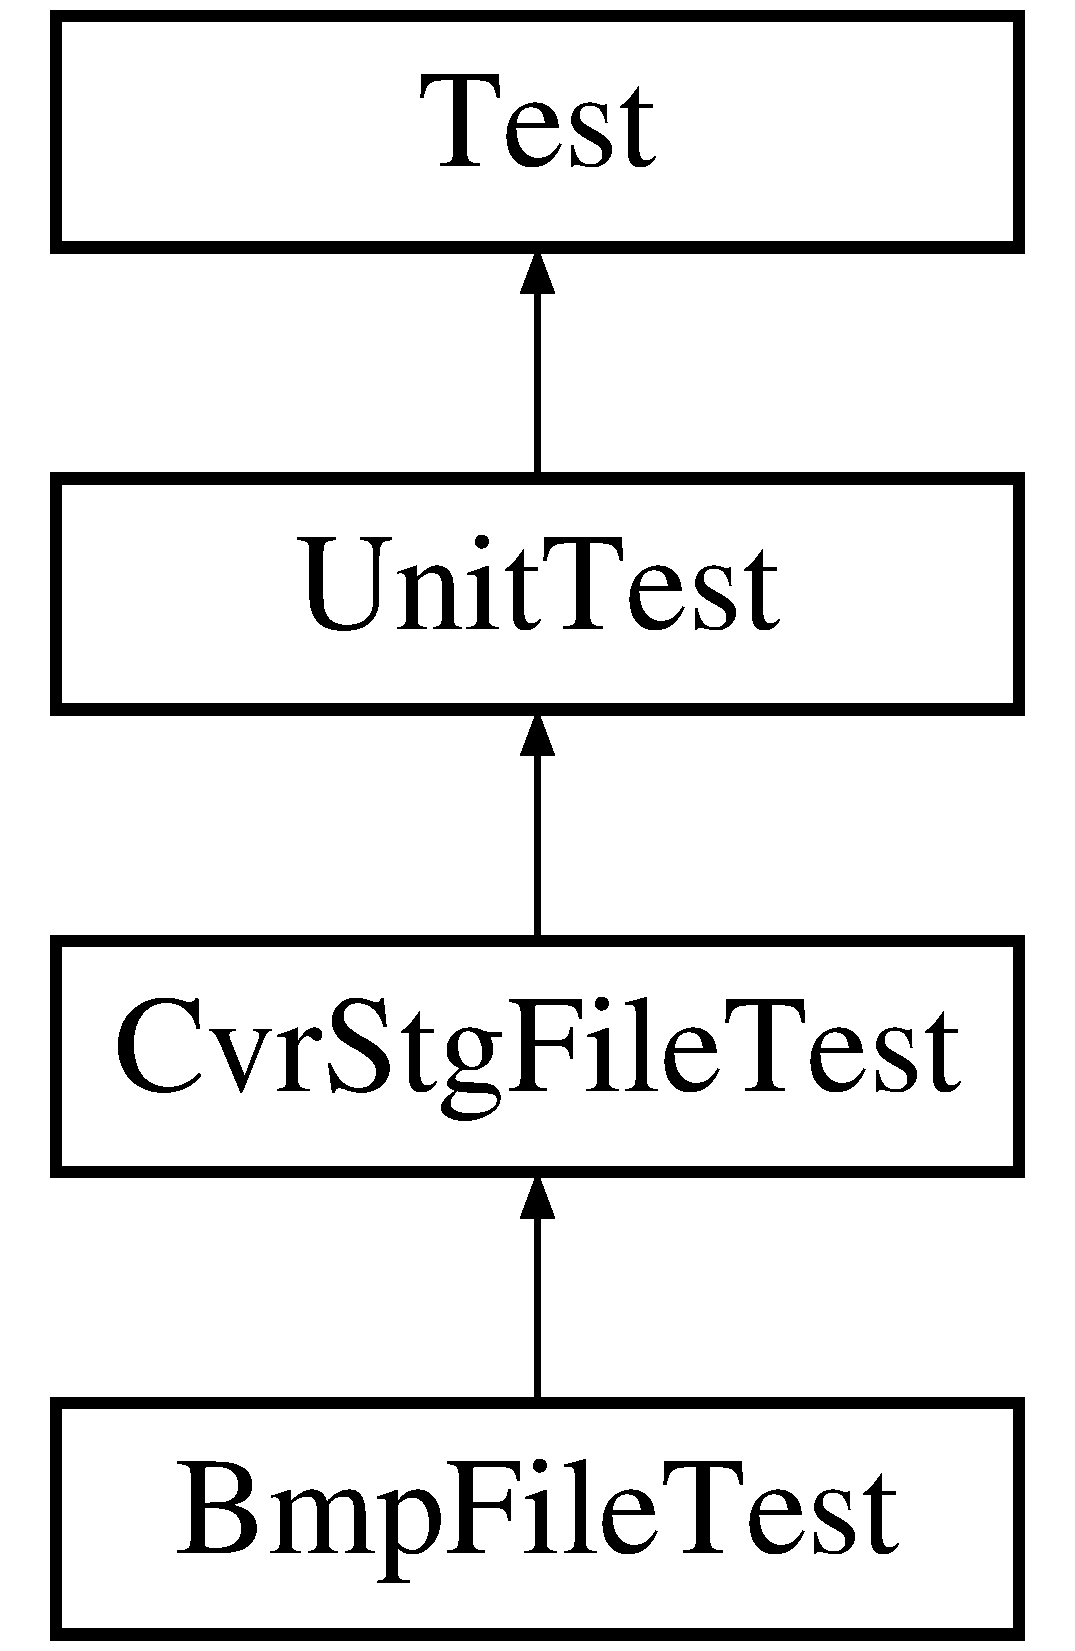
\includegraphics[height=4.000000cm]{classBmpFileTest}
\end{center}
\end{figure}
\subsection*{Public Member Functions}
\begin{DoxyCompactItemize}
\item 
\textbf{ Bmp\+File\+Test} (\textbf{ Test\+Suite} $\ast$s)
\item 
void \textbf{ setup} (void)
\item 
void \textbf{ cleanup} (void)
\item 
void \textbf{ test\+S\+V\+A\+L\+Calculation} (void)
\end{DoxyCompactItemize}
\subsection*{Private Attributes}
\begin{DoxyCompactItemize}
\item 
\textbf{ Cvr\+Stg\+File} $\ast$ \textbf{ f1}
\item 
\textbf{ Cvr\+Stg\+File} $\ast$ \textbf{ f2}
\item 
\textbf{ Graph} $\ast$ \textbf{ g1}
\item 
\textbf{ Graph} $\ast$ \textbf{ g2}
\item 
\textbf{ Selector} $\ast$ \textbf{ s1}
\item 
\textbf{ Selector} $\ast$ \textbf{ s2}
\item 
\textbf{ Bit\+String} $\ast$ \textbf{ bs1}
\item 
\textbf{ Bit\+String} $\ast$ \textbf{ bs2}
\item 
\textbf{ Globals} \textbf{ gl1}
\item 
\textbf{ Globals} \textbf{ gl2}
\end{DoxyCompactItemize}
\subsection*{Additional Inherited Members}


\subsection{Constructor \& Destructor Documentation}
\mbox{\label{classBmpFileTest_a5e70c8e9d5e9ec9a99eb0b16ea9ef616}} 
\index{Bmp\+File\+Test@{Bmp\+File\+Test}!Bmp\+File\+Test@{Bmp\+File\+Test}}
\index{Bmp\+File\+Test@{Bmp\+File\+Test}!Bmp\+File\+Test@{Bmp\+File\+Test}}
\subsubsection{Bmp\+File\+Test()}
{\footnotesize\ttfamily Bmp\+File\+Test\+::\+Bmp\+File\+Test (\begin{DoxyParamCaption}\item[{\textbf{ Test\+Suite} $\ast$}]{s }\end{DoxyParamCaption})}



\subsection{Member Function Documentation}
\mbox{\label{classBmpFileTest_a52d90560219c01c96522e3ea5927087d}} 
\index{Bmp\+File\+Test@{Bmp\+File\+Test}!cleanup@{cleanup}}
\index{cleanup@{cleanup}!Bmp\+File\+Test@{Bmp\+File\+Test}}
\subsubsection{cleanup()}
{\footnotesize\ttfamily void Bmp\+File\+Test\+::cleanup (\begin{DoxyParamCaption}\item[{void}]{ }\end{DoxyParamCaption})\hspace{0.3cm}{\ttfamily [virtual]}}

cleanup the unit test -\/ called after run 

Reimplemented from \textbf{ Unit\+Test} \doxyref{}{p.}{classUnitTest_adf77efe972ee4a766d94e3f7ddc193ad}.

\mbox{\label{classBmpFileTest_a1f3c6e5a214a2601ed28d965da436821}} 
\index{Bmp\+File\+Test@{Bmp\+File\+Test}!setup@{setup}}
\index{setup@{setup}!Bmp\+File\+Test@{Bmp\+File\+Test}}
\subsubsection{setup()}
{\footnotesize\ttfamily void Bmp\+File\+Test\+::setup (\begin{DoxyParamCaption}\item[{void}]{ }\end{DoxyParamCaption})\hspace{0.3cm}{\ttfamily [virtual]}}

setup the unit test -\/ called before run

\doxyref{Unit\+Test\+::setup}{p.}{classUnitTest_ad73fdf9012b651047ea001d21f9d27ad} will (together with \doxyref{Unit\+Test\+::cleanup}{p.}{classUnitTest_adf77efe972ee4a766d94e3f7ddc193ad}) save and restore the object stored in Globs so they should be called from the corresponding functions in the derived object if the derived unit test manipulates the Globs object. 

Reimplemented from \textbf{ Unit\+Test} \doxyref{}{p.}{classUnitTest_ad73fdf9012b651047ea001d21f9d27ad}.

\mbox{\label{classBmpFileTest_a45d9cbd414d917c10f1b94dfe9357315}} 
\index{Bmp\+File\+Test@{Bmp\+File\+Test}!test\+S\+V\+A\+L\+Calculation@{test\+S\+V\+A\+L\+Calculation}}
\index{test\+S\+V\+A\+L\+Calculation@{test\+S\+V\+A\+L\+Calculation}!Bmp\+File\+Test@{Bmp\+File\+Test}}
\subsubsection{test\+S\+V\+A\+L\+Calculation()}
{\footnotesize\ttfamily void Bmp\+File\+Test\+::test\+S\+V\+A\+L\+Calculation (\begin{DoxyParamCaption}\item[{void}]{ }\end{DoxyParamCaption})}



\subsection{Member Data Documentation}
\mbox{\label{classBmpFileTest_ae859c85f19edc8b38d5013446198352b}} 
\index{Bmp\+File\+Test@{Bmp\+File\+Test}!bs1@{bs1}}
\index{bs1@{bs1}!Bmp\+File\+Test@{Bmp\+File\+Test}}
\subsubsection{bs1}
{\footnotesize\ttfamily \textbf{ Bit\+String}$\ast$ Bmp\+File\+Test\+::bs1\hspace{0.3cm}{\ttfamily [private]}}

\mbox{\label{classBmpFileTest_a2209bb9f415263b02ee946cd6e0c2374}} 
\index{Bmp\+File\+Test@{Bmp\+File\+Test}!bs2@{bs2}}
\index{bs2@{bs2}!Bmp\+File\+Test@{Bmp\+File\+Test}}
\subsubsection{bs2}
{\footnotesize\ttfamily \textbf{ Bit\+String} $\ast$ Bmp\+File\+Test\+::bs2\hspace{0.3cm}{\ttfamily [private]}}

\mbox{\label{classBmpFileTest_a51d4702f4731f622d634ccb822afcab1}} 
\index{Bmp\+File\+Test@{Bmp\+File\+Test}!f1@{f1}}
\index{f1@{f1}!Bmp\+File\+Test@{Bmp\+File\+Test}}
\subsubsection{f1}
{\footnotesize\ttfamily \textbf{ Cvr\+Stg\+File}$\ast$ Bmp\+File\+Test\+::f1\hspace{0.3cm}{\ttfamily [private]}}

\mbox{\label{classBmpFileTest_abe38ad61c39f786a20782f3ddbb5501a}} 
\index{Bmp\+File\+Test@{Bmp\+File\+Test}!f2@{f2}}
\index{f2@{f2}!Bmp\+File\+Test@{Bmp\+File\+Test}}
\subsubsection{f2}
{\footnotesize\ttfamily \textbf{ Cvr\+Stg\+File} $\ast$ Bmp\+File\+Test\+::f2\hspace{0.3cm}{\ttfamily [private]}}

\mbox{\label{classBmpFileTest_ac193ee1bdd527581c8d9f15de3a787e0}} 
\index{Bmp\+File\+Test@{Bmp\+File\+Test}!g1@{g1}}
\index{g1@{g1}!Bmp\+File\+Test@{Bmp\+File\+Test}}
\subsubsection{g1}
{\footnotesize\ttfamily \textbf{ Graph}$\ast$ Bmp\+File\+Test\+::g1\hspace{0.3cm}{\ttfamily [private]}}

\mbox{\label{classBmpFileTest_a701f64452ff5235b8e911c7751bce234}} 
\index{Bmp\+File\+Test@{Bmp\+File\+Test}!g2@{g2}}
\index{g2@{g2}!Bmp\+File\+Test@{Bmp\+File\+Test}}
\subsubsection{g2}
{\footnotesize\ttfamily \textbf{ Graph} $\ast$ Bmp\+File\+Test\+::g2\hspace{0.3cm}{\ttfamily [private]}}

\mbox{\label{classBmpFileTest_a9d8823b33e0229cc7cceda9c1140e543}} 
\index{Bmp\+File\+Test@{Bmp\+File\+Test}!gl1@{gl1}}
\index{gl1@{gl1}!Bmp\+File\+Test@{Bmp\+File\+Test}}
\subsubsection{gl1}
{\footnotesize\ttfamily \textbf{ Globals} Bmp\+File\+Test\+::gl1\hspace{0.3cm}{\ttfamily [private]}}

\mbox{\label{classBmpFileTest_ad03b6c507745c42c886358993f2e47f3}} 
\index{Bmp\+File\+Test@{Bmp\+File\+Test}!gl2@{gl2}}
\index{gl2@{gl2}!Bmp\+File\+Test@{Bmp\+File\+Test}}
\subsubsection{gl2}
{\footnotesize\ttfamily \textbf{ Globals} Bmp\+File\+Test\+::gl2\hspace{0.3cm}{\ttfamily [private]}}

\mbox{\label{classBmpFileTest_a5029fe571788914a70d820d847f3edc7}} 
\index{Bmp\+File\+Test@{Bmp\+File\+Test}!s1@{s1}}
\index{s1@{s1}!Bmp\+File\+Test@{Bmp\+File\+Test}}
\subsubsection{s1}
{\footnotesize\ttfamily \textbf{ Selector}$\ast$ Bmp\+File\+Test\+::s1\hspace{0.3cm}{\ttfamily [private]}}

\mbox{\label{classBmpFileTest_a5dbfe43447ec11abf26719e6ff86e88d}} 
\index{Bmp\+File\+Test@{Bmp\+File\+Test}!s2@{s2}}
\index{s2@{s2}!Bmp\+File\+Test@{Bmp\+File\+Test}}
\subsubsection{s2}
{\footnotesize\ttfamily \textbf{ Selector} $\ast$ Bmp\+File\+Test\+::s2\hspace{0.3cm}{\ttfamily [private]}}



The documentation for this class was generated from the following files\+:\begin{DoxyCompactItemize}
\item 
\textbf{ Bmp\+File\+Test.\+h}\item 
\textbf{ Bmp\+File\+Test.\+cc}\end{DoxyCompactItemize}

\section{Bmp\+O\+S2\+File\+Test Class Reference}
\label{classBmpOS2FileTest}\index{Bmp\+O\+S2\+File\+Test@{Bmp\+O\+S2\+File\+Test}}


{\ttfamily \#include $<$Bmp\+O\+S2\+File\+Test.\+h$>$}

Inheritance diagram for Bmp\+O\+S2\+File\+Test\+:\begin{figure}[H]
\begin{center}
\leavevmode
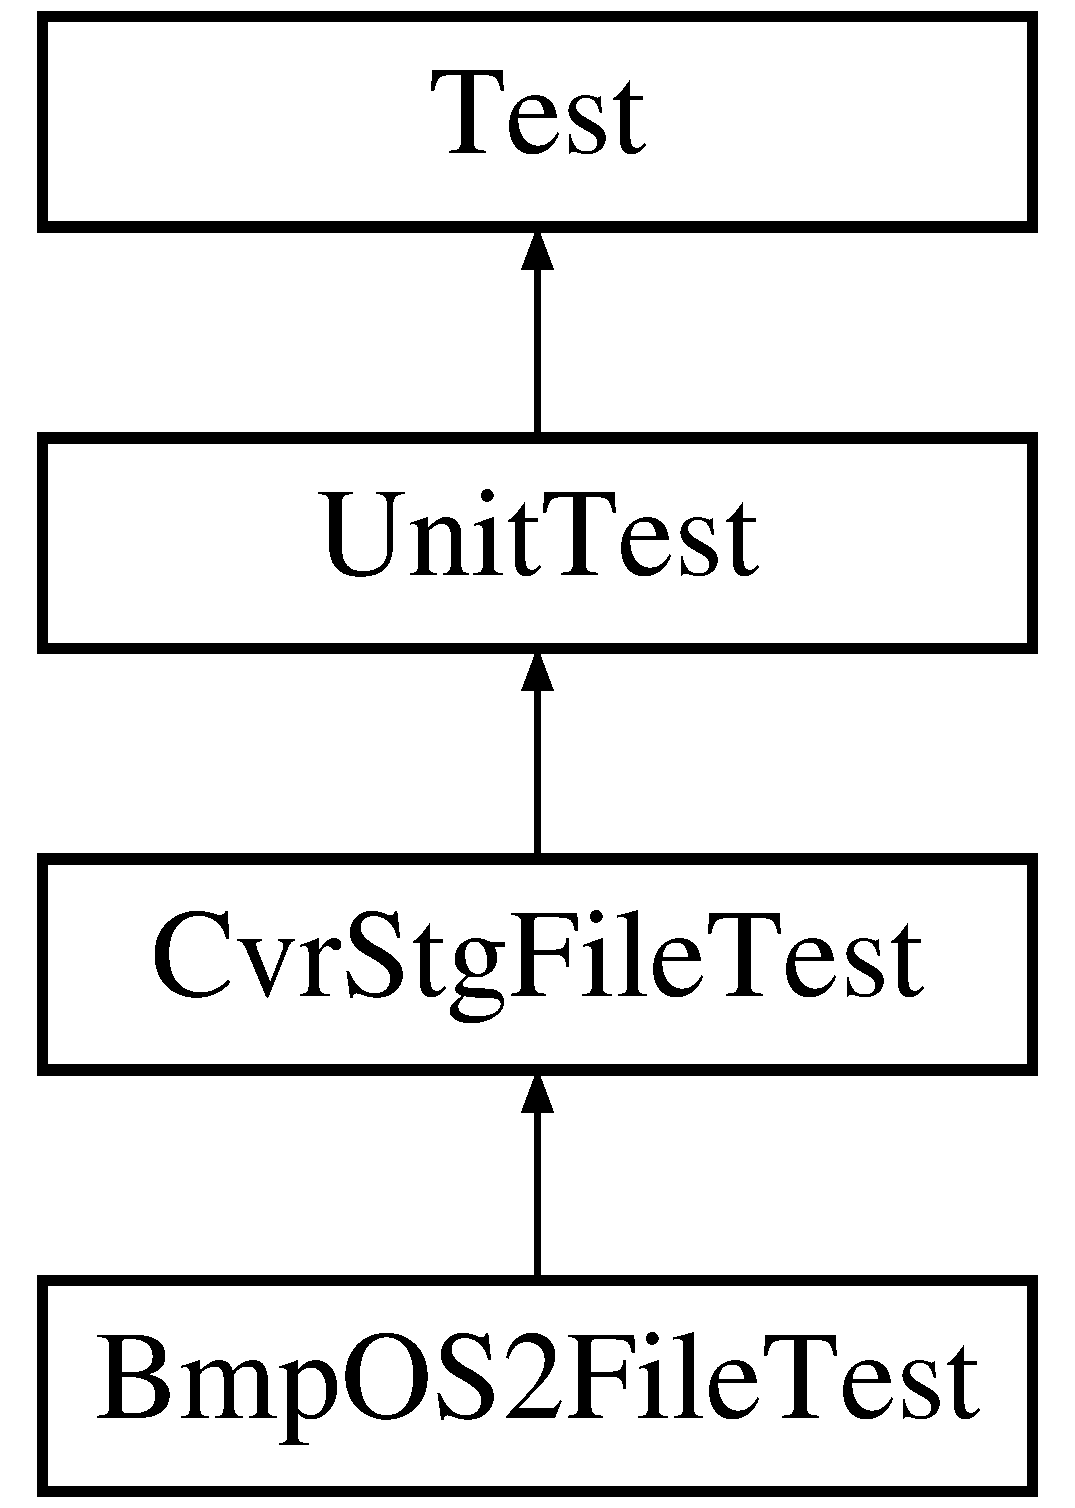
\includegraphics[height=4.000000cm]{classBmpOS2FileTest}
\end{center}
\end{figure}
\subsection*{Public Member Functions}
\begin{DoxyCompactItemize}
\item 
\textbf{ Bmp\+O\+S2\+File\+Test} (\textbf{ Test\+Suite} $\ast$s)
\item 
void \textbf{ setup} (void)
\item 
void \textbf{ cleanup} (void)
\item 
void \textbf{ test\+Read\+Write} (void)
\item 
void \textbf{ test\+Read\+Embed\+Extract} (void)
\item 
void \textbf{ test\+Read\+Embed\+Write\+Read\+Extract} (void)
\item 
void \textbf{ test\+Position} (void)
\item 
void \textbf{ test\+Read\+Extract\+Compare} (void)
\item 
void \textbf{ test\+Embedded\+Value} (void)
\end{DoxyCompactItemize}
\subsection*{Private Attributes}
\begin{DoxyCompactItemize}
\item 
\textbf{ Bit\+String} $\ast$ \textbf{ bs1}
\item 
\textbf{ Bit\+String} $\ast$ \textbf{ bs2}
\item 
\textbf{ Bit\+String} $\ast$ \textbf{ bs3}
\item 
\textbf{ Bit\+String} $\ast$ \textbf{ bs4}
\item 
\textbf{ Cvr\+Stg\+File} $\ast$ \textbf{ f1}
\item 
\textbf{ Cvr\+Stg\+File} $\ast$ \textbf{ f2}
\item 
\textbf{ Cvr\+Stg\+File} $\ast$ \textbf{ f3}
\item 
\textbf{ Cvr\+Stg\+File} $\ast$ \textbf{ f4}
\item 
\textbf{ Globals} \textbf{ gl1}
\item 
\textbf{ Globals} \textbf{ gl2}
\item 
\textbf{ Globals} \textbf{ gl3}
\item 
\textbf{ Globals} \textbf{ gl4}
\end{DoxyCompactItemize}
\subsection*{Additional Inherited Members}


\subsection{Constructor \& Destructor Documentation}
\mbox{\label{classBmpOS2FileTest_a0a63a4d4e958ff6f63bd8b0493f3bb91}} 
\index{Bmp\+O\+S2\+File\+Test@{Bmp\+O\+S2\+File\+Test}!Bmp\+O\+S2\+File\+Test@{Bmp\+O\+S2\+File\+Test}}
\index{Bmp\+O\+S2\+File\+Test@{Bmp\+O\+S2\+File\+Test}!Bmp\+O\+S2\+File\+Test@{Bmp\+O\+S2\+File\+Test}}
\subsubsection{Bmp\+O\+S2\+File\+Test()}
{\footnotesize\ttfamily Bmp\+O\+S2\+File\+Test\+::\+Bmp\+O\+S2\+File\+Test (\begin{DoxyParamCaption}\item[{\textbf{ Test\+Suite} $\ast$}]{s }\end{DoxyParamCaption})}



\subsection{Member Function Documentation}
\mbox{\label{classBmpOS2FileTest_a1fcfaa4f555c1cdf8c6ff2fc8e451eec}} 
\index{Bmp\+O\+S2\+File\+Test@{Bmp\+O\+S2\+File\+Test}!cleanup@{cleanup}}
\index{cleanup@{cleanup}!Bmp\+O\+S2\+File\+Test@{Bmp\+O\+S2\+File\+Test}}
\subsubsection{cleanup()}
{\footnotesize\ttfamily void Bmp\+O\+S2\+File\+Test\+::cleanup (\begin{DoxyParamCaption}\item[{void}]{ }\end{DoxyParamCaption})\hspace{0.3cm}{\ttfamily [virtual]}}

cleanup the unit test -\/ called after run 

Reimplemented from \textbf{ Unit\+Test} \doxyref{}{p.}{classUnitTest_adf77efe972ee4a766d94e3f7ddc193ad}.

\mbox{\label{classBmpOS2FileTest_aa2a4aa30f613dff18079f04a45ee6665}} 
\index{Bmp\+O\+S2\+File\+Test@{Bmp\+O\+S2\+File\+Test}!setup@{setup}}
\index{setup@{setup}!Bmp\+O\+S2\+File\+Test@{Bmp\+O\+S2\+File\+Test}}
\subsubsection{setup()}
{\footnotesize\ttfamily void Bmp\+O\+S2\+File\+Test\+::setup (\begin{DoxyParamCaption}\item[{void}]{ }\end{DoxyParamCaption})\hspace{0.3cm}{\ttfamily [virtual]}}

setup the unit test -\/ called before run

\doxyref{Unit\+Test\+::setup}{p.}{classUnitTest_ad73fdf9012b651047ea001d21f9d27ad} will (together with \doxyref{Unit\+Test\+::cleanup}{p.}{classUnitTest_adf77efe972ee4a766d94e3f7ddc193ad}) save and restore the object stored in Globs so they should be called from the corresponding functions in the derived object if the derived unit test manipulates the Globs object. 

Reimplemented from \textbf{ Unit\+Test} \doxyref{}{p.}{classUnitTest_ad73fdf9012b651047ea001d21f9d27ad}.

\mbox{\label{classBmpOS2FileTest_ac9027ac14a0cbf39ecada214d4048280}} 
\index{Bmp\+O\+S2\+File\+Test@{Bmp\+O\+S2\+File\+Test}!test\+Embedded\+Value@{test\+Embedded\+Value}}
\index{test\+Embedded\+Value@{test\+Embedded\+Value}!Bmp\+O\+S2\+File\+Test@{Bmp\+O\+S2\+File\+Test}}
\subsubsection{test\+Embedded\+Value()}
{\footnotesize\ttfamily void Bmp\+O\+S2\+File\+Test\+::test\+Embedded\+Value (\begin{DoxyParamCaption}\item[{void}]{ }\end{DoxyParamCaption})}

\mbox{\label{classBmpOS2FileTest_a3d235c9267b76959b8bee32b8fcefb40}} 
\index{Bmp\+O\+S2\+File\+Test@{Bmp\+O\+S2\+File\+Test}!test\+Position@{test\+Position}}
\index{test\+Position@{test\+Position}!Bmp\+O\+S2\+File\+Test@{Bmp\+O\+S2\+File\+Test}}
\subsubsection{test\+Position()}
{\footnotesize\ttfamily void Bmp\+O\+S2\+File\+Test\+::test\+Position (\begin{DoxyParamCaption}\item[{void}]{ }\end{DoxyParamCaption})}

\mbox{\label{classBmpOS2FileTest_a53f0d78d0fe60de31911cddb325a39eb}} 
\index{Bmp\+O\+S2\+File\+Test@{Bmp\+O\+S2\+File\+Test}!test\+Read\+Embed\+Extract@{test\+Read\+Embed\+Extract}}
\index{test\+Read\+Embed\+Extract@{test\+Read\+Embed\+Extract}!Bmp\+O\+S2\+File\+Test@{Bmp\+O\+S2\+File\+Test}}
\subsubsection{test\+Read\+Embed\+Extract()}
{\footnotesize\ttfamily void Bmp\+O\+S2\+File\+Test\+::test\+Read\+Embed\+Extract (\begin{DoxyParamCaption}\item[{void}]{ }\end{DoxyParamCaption})}

\mbox{\label{classBmpOS2FileTest_ae4e0f7fc89794a74e03bbbf006978f61}} 
\index{Bmp\+O\+S2\+File\+Test@{Bmp\+O\+S2\+File\+Test}!test\+Read\+Embed\+Write\+Read\+Extract@{test\+Read\+Embed\+Write\+Read\+Extract}}
\index{test\+Read\+Embed\+Write\+Read\+Extract@{test\+Read\+Embed\+Write\+Read\+Extract}!Bmp\+O\+S2\+File\+Test@{Bmp\+O\+S2\+File\+Test}}
\subsubsection{test\+Read\+Embed\+Write\+Read\+Extract()}
{\footnotesize\ttfamily void Bmp\+O\+S2\+File\+Test\+::test\+Read\+Embed\+Write\+Read\+Extract (\begin{DoxyParamCaption}\item[{void}]{ }\end{DoxyParamCaption})}

\mbox{\label{classBmpOS2FileTest_a4e62e6870b8d2cc5bb2b5f6ae402abe6}} 
\index{Bmp\+O\+S2\+File\+Test@{Bmp\+O\+S2\+File\+Test}!test\+Read\+Extract\+Compare@{test\+Read\+Extract\+Compare}}
\index{test\+Read\+Extract\+Compare@{test\+Read\+Extract\+Compare}!Bmp\+O\+S2\+File\+Test@{Bmp\+O\+S2\+File\+Test}}
\subsubsection{test\+Read\+Extract\+Compare()}
{\footnotesize\ttfamily void Bmp\+O\+S2\+File\+Test\+::test\+Read\+Extract\+Compare (\begin{DoxyParamCaption}\item[{void}]{ }\end{DoxyParamCaption})}

\mbox{\label{classBmpOS2FileTest_ac3a8059096148685311f10836c172d3d}} 
\index{Bmp\+O\+S2\+File\+Test@{Bmp\+O\+S2\+File\+Test}!test\+Read\+Write@{test\+Read\+Write}}
\index{test\+Read\+Write@{test\+Read\+Write}!Bmp\+O\+S2\+File\+Test@{Bmp\+O\+S2\+File\+Test}}
\subsubsection{test\+Read\+Write()}
{\footnotesize\ttfamily void Bmp\+O\+S2\+File\+Test\+::test\+Read\+Write (\begin{DoxyParamCaption}\item[{void}]{ }\end{DoxyParamCaption})}



\subsection{Member Data Documentation}
\mbox{\label{classBmpOS2FileTest_a1f9f06cdab685d1619ce0cf71f78032f}} 
\index{Bmp\+O\+S2\+File\+Test@{Bmp\+O\+S2\+File\+Test}!bs1@{bs1}}
\index{bs1@{bs1}!Bmp\+O\+S2\+File\+Test@{Bmp\+O\+S2\+File\+Test}}
\subsubsection{bs1}
{\footnotesize\ttfamily \textbf{ Bit\+String}$\ast$ Bmp\+O\+S2\+File\+Test\+::bs1\hspace{0.3cm}{\ttfamily [private]}}

\mbox{\label{classBmpOS2FileTest_ac0fedf91338a227d2800e79d28d0ae77}} 
\index{Bmp\+O\+S2\+File\+Test@{Bmp\+O\+S2\+File\+Test}!bs2@{bs2}}
\index{bs2@{bs2}!Bmp\+O\+S2\+File\+Test@{Bmp\+O\+S2\+File\+Test}}
\subsubsection{bs2}
{\footnotesize\ttfamily \textbf{ Bit\+String} $\ast$ Bmp\+O\+S2\+File\+Test\+::bs2\hspace{0.3cm}{\ttfamily [private]}}

\mbox{\label{classBmpOS2FileTest_a24c42ae78ff894065277806fa429f46e}} 
\index{Bmp\+O\+S2\+File\+Test@{Bmp\+O\+S2\+File\+Test}!bs3@{bs3}}
\index{bs3@{bs3}!Bmp\+O\+S2\+File\+Test@{Bmp\+O\+S2\+File\+Test}}
\subsubsection{bs3}
{\footnotesize\ttfamily \textbf{ Bit\+String} $\ast$ Bmp\+O\+S2\+File\+Test\+::bs3\hspace{0.3cm}{\ttfamily [private]}}

\mbox{\label{classBmpOS2FileTest_a907304a0224acd6d94378232b695b7cd}} 
\index{Bmp\+O\+S2\+File\+Test@{Bmp\+O\+S2\+File\+Test}!bs4@{bs4}}
\index{bs4@{bs4}!Bmp\+O\+S2\+File\+Test@{Bmp\+O\+S2\+File\+Test}}
\subsubsection{bs4}
{\footnotesize\ttfamily \textbf{ Bit\+String} $\ast$ Bmp\+O\+S2\+File\+Test\+::bs4\hspace{0.3cm}{\ttfamily [private]}}

\mbox{\label{classBmpOS2FileTest_a09fc57f7a850e0d7b4ebac7c24045104}} 
\index{Bmp\+O\+S2\+File\+Test@{Bmp\+O\+S2\+File\+Test}!f1@{f1}}
\index{f1@{f1}!Bmp\+O\+S2\+File\+Test@{Bmp\+O\+S2\+File\+Test}}
\subsubsection{f1}
{\footnotesize\ttfamily \textbf{ Cvr\+Stg\+File}$\ast$ Bmp\+O\+S2\+File\+Test\+::f1\hspace{0.3cm}{\ttfamily [private]}}

\mbox{\label{classBmpOS2FileTest_a33bf41aa2fe689ebd6327caa231ff946}} 
\index{Bmp\+O\+S2\+File\+Test@{Bmp\+O\+S2\+File\+Test}!f2@{f2}}
\index{f2@{f2}!Bmp\+O\+S2\+File\+Test@{Bmp\+O\+S2\+File\+Test}}
\subsubsection{f2}
{\footnotesize\ttfamily \textbf{ Cvr\+Stg\+File} $\ast$ Bmp\+O\+S2\+File\+Test\+::f2\hspace{0.3cm}{\ttfamily [private]}}

\mbox{\label{classBmpOS2FileTest_a6671840f4e885cef64c8558036d5e610}} 
\index{Bmp\+O\+S2\+File\+Test@{Bmp\+O\+S2\+File\+Test}!f3@{f3}}
\index{f3@{f3}!Bmp\+O\+S2\+File\+Test@{Bmp\+O\+S2\+File\+Test}}
\subsubsection{f3}
{\footnotesize\ttfamily \textbf{ Cvr\+Stg\+File} $\ast$ Bmp\+O\+S2\+File\+Test\+::f3\hspace{0.3cm}{\ttfamily [private]}}

\mbox{\label{classBmpOS2FileTest_aef99bf83500f7429b74094c880444223}} 
\index{Bmp\+O\+S2\+File\+Test@{Bmp\+O\+S2\+File\+Test}!f4@{f4}}
\index{f4@{f4}!Bmp\+O\+S2\+File\+Test@{Bmp\+O\+S2\+File\+Test}}
\subsubsection{f4}
{\footnotesize\ttfamily \textbf{ Cvr\+Stg\+File} $\ast$ Bmp\+O\+S2\+File\+Test\+::f4\hspace{0.3cm}{\ttfamily [private]}}

\mbox{\label{classBmpOS2FileTest_a62b43b7bff6c5a28de3b8493396f294f}} 
\index{Bmp\+O\+S2\+File\+Test@{Bmp\+O\+S2\+File\+Test}!gl1@{gl1}}
\index{gl1@{gl1}!Bmp\+O\+S2\+File\+Test@{Bmp\+O\+S2\+File\+Test}}
\subsubsection{gl1}
{\footnotesize\ttfamily \textbf{ Globals} Bmp\+O\+S2\+File\+Test\+::gl1\hspace{0.3cm}{\ttfamily [private]}}

\mbox{\label{classBmpOS2FileTest_af40bb63eeb0e97ffb6906417aee8646a}} 
\index{Bmp\+O\+S2\+File\+Test@{Bmp\+O\+S2\+File\+Test}!gl2@{gl2}}
\index{gl2@{gl2}!Bmp\+O\+S2\+File\+Test@{Bmp\+O\+S2\+File\+Test}}
\subsubsection{gl2}
{\footnotesize\ttfamily \textbf{ Globals} Bmp\+O\+S2\+File\+Test\+::gl2\hspace{0.3cm}{\ttfamily [private]}}

\mbox{\label{classBmpOS2FileTest_a3406fa49eeb3eda4a25344adfe261718}} 
\index{Bmp\+O\+S2\+File\+Test@{Bmp\+O\+S2\+File\+Test}!gl3@{gl3}}
\index{gl3@{gl3}!Bmp\+O\+S2\+File\+Test@{Bmp\+O\+S2\+File\+Test}}
\subsubsection{gl3}
{\footnotesize\ttfamily \textbf{ Globals} Bmp\+O\+S2\+File\+Test\+::gl3\hspace{0.3cm}{\ttfamily [private]}}

\mbox{\label{classBmpOS2FileTest_a08abc87034baa11df03d956aaf4bf65c}} 
\index{Bmp\+O\+S2\+File\+Test@{Bmp\+O\+S2\+File\+Test}!gl4@{gl4}}
\index{gl4@{gl4}!Bmp\+O\+S2\+File\+Test@{Bmp\+O\+S2\+File\+Test}}
\subsubsection{gl4}
{\footnotesize\ttfamily \textbf{ Globals} Bmp\+O\+S2\+File\+Test\+::gl4\hspace{0.3cm}{\ttfamily [private]}}



The documentation for this class was generated from the following files\+:\begin{DoxyCompactItemize}
\item 
\textbf{ Bmp\+O\+S2\+File\+Test.\+h}\item 
\textbf{ Bmp\+O\+S2\+File\+Test.\+cc}\end{DoxyCompactItemize}

\section{Bmp\+Palette\+Sample\+Value Class Reference}
\label{classBmpPaletteSampleValue}\index{Bmp\+Palette\+Sample\+Value@{Bmp\+Palette\+Sample\+Value}}


a sample in a bmp palette (i.\+e. in a 1-\/,4-\/ or 8-\/bit) file  




{\ttfamily \#include $<$Bmp\+Palette\+Sample\+Value.\+h$>$}

Inheritance diagram for Bmp\+Palette\+Sample\+Value\+:\begin{figure}[H]
\begin{center}
\leavevmode
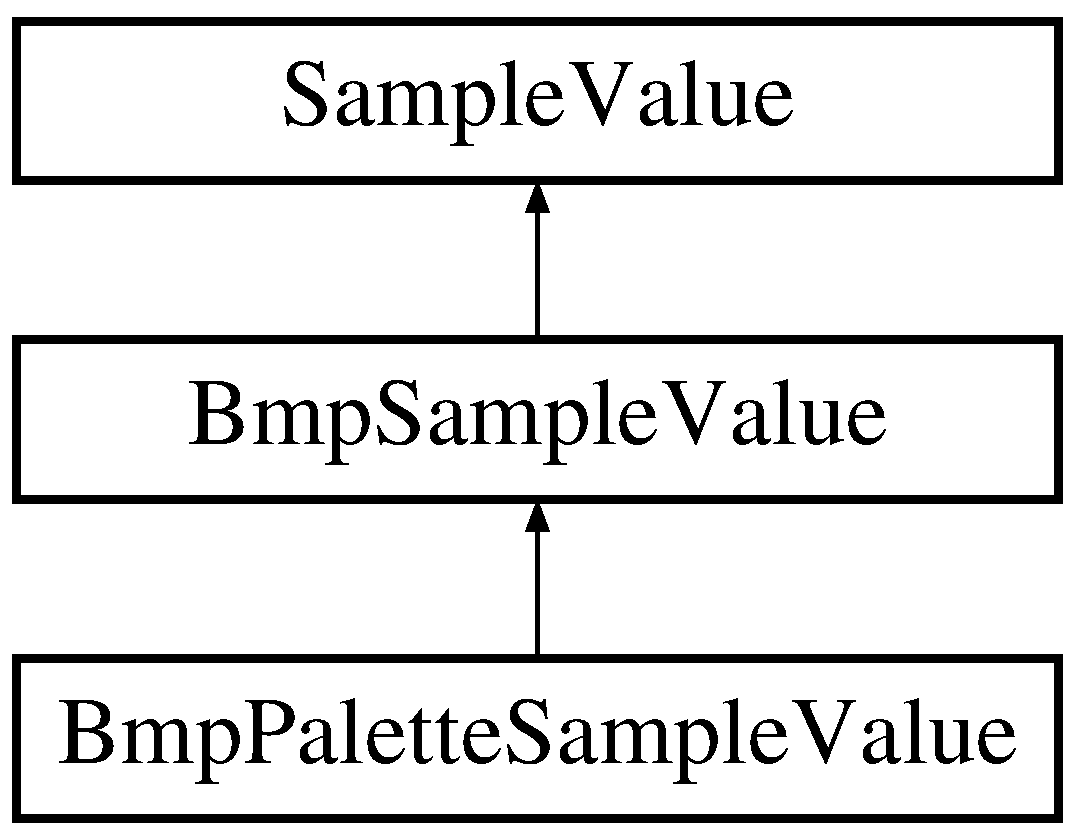
\includegraphics[height=3.000000cm]{classBmpPaletteSampleValue}
\end{center}
\end{figure}
\subsection*{Public Member Functions}
\begin{DoxyCompactItemize}
\item 
\textbf{ Bmp\+Palette\+Sample\+Value} (\textbf{ B\+Y\+TE} i)
\item 
\textbf{ Sample\+Value} $\ast$ \textbf{ get\+Nearest\+Target\+Sample\+Value} (\textbf{ Emb\+Value} t) const
\item 
std\+::string \textbf{ get\+Name} (void) const
\item 
\textbf{ B\+Y\+TE} \textbf{ get\+Index} (void) const
\item 
\textbf{ B\+Y\+TE} \textbf{ get\+Red} (void) const
\item 
\textbf{ B\+Y\+TE} \textbf{ get\+Green} (void) const
\item 
\textbf{ B\+Y\+TE} \textbf{ get\+Blue} (void) const
\end{DoxyCompactItemize}
\subsection*{Private Member Functions}
\begin{DoxyCompactItemize}
\item 
\textbf{ Emb\+Value} \textbf{ calc\+E\+Value} (\textbf{ B\+Y\+TE} idx) const
\end{DoxyCompactItemize}
\subsection*{Private Attributes}
\begin{DoxyCompactItemize}
\item 
\textbf{ Color\+Palette} $\ast$ \textbf{ Palette}
\item 
\textbf{ B\+Y\+TE} \textbf{ Index}
\end{DoxyCompactItemize}
\subsection*{Additional Inherited Members}


\subsection{Constructor \& Destructor Documentation}
\mbox{\label{classBmpPaletteSampleValue_a81d345b74502effc44a9995ab44918ed}} 
\index{Bmp\+Palette\+Sample\+Value@{Bmp\+Palette\+Sample\+Value}!Bmp\+Palette\+Sample\+Value@{Bmp\+Palette\+Sample\+Value}}
\index{Bmp\+Palette\+Sample\+Value@{Bmp\+Palette\+Sample\+Value}!Bmp\+Palette\+Sample\+Value@{Bmp\+Palette\+Sample\+Value}}
\subsubsection{Bmp\+Palette\+Sample\+Value()}
{\footnotesize\ttfamily Bmp\+Palette\+Sample\+Value\+::\+Bmp\+Palette\+Sample\+Value (\begin{DoxyParamCaption}\item[{\textbf{ B\+Y\+TE}}]{i }\end{DoxyParamCaption})}



\subsection{Member Function Documentation}
\mbox{\label{classBmpPaletteSampleValue_a480da9a02dff7cab6b10278cdf2d25d9}} 
\index{Bmp\+Palette\+Sample\+Value@{Bmp\+Palette\+Sample\+Value}!calc\+E\+Value@{calc\+E\+Value}}
\index{calc\+E\+Value@{calc\+E\+Value}!Bmp\+Palette\+Sample\+Value@{Bmp\+Palette\+Sample\+Value}}
\subsubsection{calc\+E\+Value()}
{\footnotesize\ttfamily \textbf{ Emb\+Value} Bmp\+Palette\+Sample\+Value\+::calc\+E\+Value (\begin{DoxyParamCaption}\item[{\textbf{ B\+Y\+TE}}]{idx }\end{DoxyParamCaption}) const\hspace{0.3cm}{\ttfamily [inline]}, {\ttfamily [private]}}

\mbox{\label{classBmpPaletteSampleValue_aba2549aa10e39b580488e0c4625720c0}} 
\index{Bmp\+Palette\+Sample\+Value@{Bmp\+Palette\+Sample\+Value}!get\+Blue@{get\+Blue}}
\index{get\+Blue@{get\+Blue}!Bmp\+Palette\+Sample\+Value@{Bmp\+Palette\+Sample\+Value}}
\subsubsection{get\+Blue()}
{\footnotesize\ttfamily \textbf{ B\+Y\+TE} Bmp\+Palette\+Sample\+Value\+::get\+Blue (\begin{DoxyParamCaption}\item[{void}]{ }\end{DoxyParamCaption}) const\hspace{0.3cm}{\ttfamily [inline]}, {\ttfamily [virtual]}}

get the blue color component 

Implements \textbf{ Bmp\+Sample\+Value} \doxyref{}{p.}{classBmpSampleValue_a0c31d4428158c7c6017935ac03254b26}.

\mbox{\label{classBmpPaletteSampleValue_a886c54100ed64d4bfd732b4be4ddae67}} 
\index{Bmp\+Palette\+Sample\+Value@{Bmp\+Palette\+Sample\+Value}!get\+Green@{get\+Green}}
\index{get\+Green@{get\+Green}!Bmp\+Palette\+Sample\+Value@{Bmp\+Palette\+Sample\+Value}}
\subsubsection{get\+Green()}
{\footnotesize\ttfamily \textbf{ B\+Y\+TE} Bmp\+Palette\+Sample\+Value\+::get\+Green (\begin{DoxyParamCaption}\item[{void}]{ }\end{DoxyParamCaption}) const\hspace{0.3cm}{\ttfamily [inline]}, {\ttfamily [virtual]}}

get the green color component 

Implements \textbf{ Bmp\+Sample\+Value} \doxyref{}{p.}{classBmpSampleValue_a5d646a4082648a5b63323167553066ab}.

\mbox{\label{classBmpPaletteSampleValue_aaaae1fc0c04018c029e923c8c1a04d86}} 
\index{Bmp\+Palette\+Sample\+Value@{Bmp\+Palette\+Sample\+Value}!get\+Index@{get\+Index}}
\index{get\+Index@{get\+Index}!Bmp\+Palette\+Sample\+Value@{Bmp\+Palette\+Sample\+Value}}
\subsubsection{get\+Index()}
{\footnotesize\ttfamily \textbf{ B\+Y\+TE} Bmp\+Palette\+Sample\+Value\+::get\+Index (\begin{DoxyParamCaption}\item[{void}]{ }\end{DoxyParamCaption}) const\hspace{0.3cm}{\ttfamily [inline]}}

\mbox{\label{classBmpPaletteSampleValue_afdee36c56b6cc471c96d93dbbc8c8fa0}} 
\index{Bmp\+Palette\+Sample\+Value@{Bmp\+Palette\+Sample\+Value}!get\+Name@{get\+Name}}
\index{get\+Name@{get\+Name}!Bmp\+Palette\+Sample\+Value@{Bmp\+Palette\+Sample\+Value}}
\subsubsection{get\+Name()}
{\footnotesize\ttfamily std\+::string Bmp\+Palette\+Sample\+Value\+::get\+Name (\begin{DoxyParamCaption}\item[{void}]{ }\end{DoxyParamCaption}) const\hspace{0.3cm}{\ttfamily [virtual]}}

return a short name uniquely identifying this sample value 

Implements \textbf{ Sample\+Value} \doxyref{}{p.}{classSampleValue_aeaf5c46ec6d023840e9773604b20d25c}.

\mbox{\label{classBmpPaletteSampleValue_acb0da2ffb8ad2b8880e5eb8d0ea16e62}} 
\index{Bmp\+Palette\+Sample\+Value@{Bmp\+Palette\+Sample\+Value}!get\+Nearest\+Target\+Sample\+Value@{get\+Nearest\+Target\+Sample\+Value}}
\index{get\+Nearest\+Target\+Sample\+Value@{get\+Nearest\+Target\+Sample\+Value}!Bmp\+Palette\+Sample\+Value@{Bmp\+Palette\+Sample\+Value}}
\subsubsection{get\+Nearest\+Target\+Sample\+Value()}
{\footnotesize\ttfamily \textbf{ Sample\+Value} $\ast$ Bmp\+Palette\+Sample\+Value\+::get\+Nearest\+Target\+Sample\+Value (\begin{DoxyParamCaption}\item[{\textbf{ Emb\+Value}}]{t }\end{DoxyParamCaption}) const\hspace{0.3cm}{\ttfamily [virtual]}}

get the nearest (with the least distance to this sample value) sample value whose embedded value equals the specified target 
\begin{DoxyParams}{Parameters}
{\em t} & the target embedded value\\
\hline
\end{DoxyParams}
If two or more target sample values have equal distance each of them should be returned with equal probability.

The returned \doxyref{Sample\+Value}{p.}{classSampleValue} object should be deleted by the callser. 

Implements \textbf{ Sample\+Value} \doxyref{}{p.}{classSampleValue_aeca3fc1fd34c09d2244706b010935c2c}.

\mbox{\label{classBmpPaletteSampleValue_a168e95b6da4f8aa4216fde934d561660}} 
\index{Bmp\+Palette\+Sample\+Value@{Bmp\+Palette\+Sample\+Value}!get\+Red@{get\+Red}}
\index{get\+Red@{get\+Red}!Bmp\+Palette\+Sample\+Value@{Bmp\+Palette\+Sample\+Value}}
\subsubsection{get\+Red()}
{\footnotesize\ttfamily \textbf{ B\+Y\+TE} Bmp\+Palette\+Sample\+Value\+::get\+Red (\begin{DoxyParamCaption}\item[{void}]{ }\end{DoxyParamCaption}) const\hspace{0.3cm}{\ttfamily [inline]}, {\ttfamily [virtual]}}

get the red color component 

Implements \textbf{ Bmp\+Sample\+Value} \doxyref{}{p.}{classBmpSampleValue_a8665a4c4db9ac910abf4ec0738cfde68}.



\subsection{Member Data Documentation}
\mbox{\label{classBmpPaletteSampleValue_ac838911edfa68d87a10580e098e6e353}} 
\index{Bmp\+Palette\+Sample\+Value@{Bmp\+Palette\+Sample\+Value}!Index@{Index}}
\index{Index@{Index}!Bmp\+Palette\+Sample\+Value@{Bmp\+Palette\+Sample\+Value}}
\subsubsection{Index}
{\footnotesize\ttfamily \textbf{ B\+Y\+TE} Bmp\+Palette\+Sample\+Value\+::\+Index\hspace{0.3cm}{\ttfamily [private]}}

\mbox{\label{classBmpPaletteSampleValue_af9a9aae8c5ce9dfd8e2566d984cf7302}} 
\index{Bmp\+Palette\+Sample\+Value@{Bmp\+Palette\+Sample\+Value}!Palette@{Palette}}
\index{Palette@{Palette}!Bmp\+Palette\+Sample\+Value@{Bmp\+Palette\+Sample\+Value}}
\subsubsection{Palette}
{\footnotesize\ttfamily \textbf{ Color\+Palette}$\ast$ Bmp\+Palette\+Sample\+Value\+::\+Palette\hspace{0.3cm}{\ttfamily [private]}}



The documentation for this class was generated from the following files\+:\begin{DoxyCompactItemize}
\item 
\textbf{ Bmp\+Palette\+Sample\+Value.\+h}\item 
\textbf{ Bmp\+Palette\+Sample\+Value.\+cc}\end{DoxyCompactItemize}

\section{Bmp\+Palette\+Sample\+Value\+Test Class Reference}
\label{classBmpPaletteSampleValueTest}\index{Bmp\+Palette\+Sample\+Value\+Test@{Bmp\+Palette\+Sample\+Value\+Test}}


{\ttfamily \#include $<$Bmp\+Palette\+Sample\+Value\+Test.\+h$>$}

Inheritance diagram for Bmp\+Palette\+Sample\+Value\+Test\+:\begin{figure}[H]
\begin{center}
\leavevmode
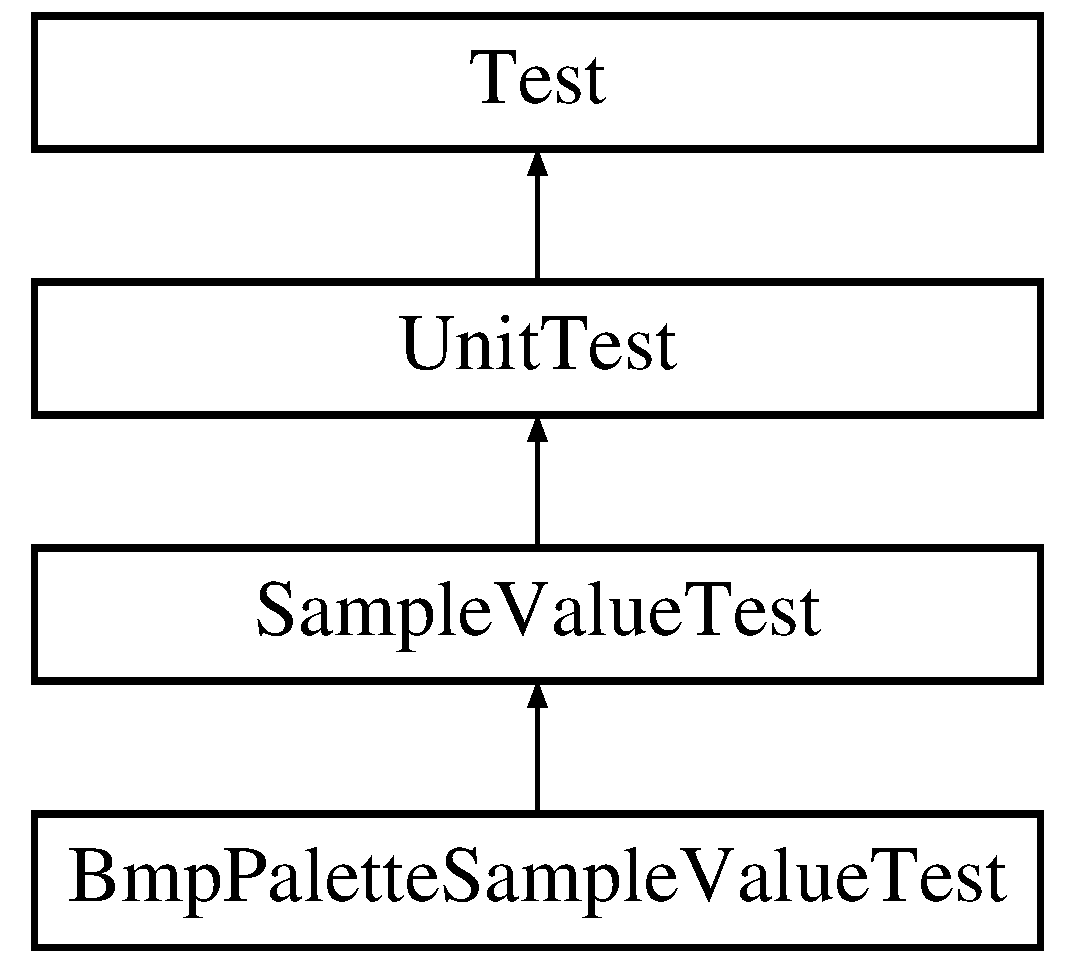
\includegraphics[height=4.000000cm]{classBmpPaletteSampleValueTest}
\end{center}
\end{figure}
\subsection*{Public Member Functions}
\begin{DoxyCompactItemize}
\item 
\textbf{ Bmp\+Palette\+Sample\+Value\+Test} (\textbf{ Test\+Suite} $\ast$s)
\item 
void \textbf{ setup} (void)
\item 
void \textbf{ cleanup} (void)
\item 
void \textbf{ test\+Distance} (void)
\item 
void \textbf{ test\+Is\+Neighbour} (void)
\end{DoxyCompactItemize}
\subsection*{Private Attributes}
\begin{DoxyCompactItemize}
\item 
\textbf{ Cvr\+Stg\+File} $\ast$ \textbf{ f1}
\item 
\textbf{ Cvr\+Stg\+File} $\ast$ \textbf{ f2}
\item 
\textbf{ Globals} \textbf{ gl1}
\item 
\textbf{ Globals} \textbf{ gl2}
\item 
\textbf{ Sample\+Value} $\ast$ \textbf{ sv1\+\_\+0}
\item 
\textbf{ Sample\+Value} $\ast$ \textbf{ sv1\+\_\+3}
\item 
\textbf{ Sample\+Value} $\ast$ \textbf{ sv1\+\_\+7}
\item 
\textbf{ Sample\+Value} $\ast$ \textbf{ sv1\+\_\+15}
\item 
\textbf{ Sample\+Value} $\ast$ \textbf{ sv2\+\_\+3\+\_\+49\+\_\+96\+\_\+5}
\item 
\textbf{ Sample\+Value} $\ast$ \textbf{ sv2\+\_\+10\+\_\+11\+\_\+99\+\_\+203}
\item 
\textbf{ Sample\+Value} $\ast$ \textbf{ sv2\+\_\+48\+\_\+18\+\_\+106\+\_\+194}
\item 
\textbf{ Sample\+Value} $\ast$ \textbf{ sv2\+\_\+68\+\_\+73\+\_\+104\+\_\+15}
\item 
\textbf{ Sample\+Value} $\ast$ \textbf{ sv2\+\_\+171\+\_\+61\+\_\+97\+\_\+25}
\end{DoxyCompactItemize}
\subsection*{Additional Inherited Members}


\subsection{Constructor \& Destructor Documentation}
\mbox{\label{classBmpPaletteSampleValueTest_ae24226179c79bb4a99f429779c441aa6}} 
\index{Bmp\+Palette\+Sample\+Value\+Test@{Bmp\+Palette\+Sample\+Value\+Test}!Bmp\+Palette\+Sample\+Value\+Test@{Bmp\+Palette\+Sample\+Value\+Test}}
\index{Bmp\+Palette\+Sample\+Value\+Test@{Bmp\+Palette\+Sample\+Value\+Test}!Bmp\+Palette\+Sample\+Value\+Test@{Bmp\+Palette\+Sample\+Value\+Test}}
\subsubsection{Bmp\+Palette\+Sample\+Value\+Test()}
{\footnotesize\ttfamily Bmp\+Palette\+Sample\+Value\+Test\+::\+Bmp\+Palette\+Sample\+Value\+Test (\begin{DoxyParamCaption}\item[{\textbf{ Test\+Suite} $\ast$}]{s }\end{DoxyParamCaption})}



\subsection{Member Function Documentation}
\mbox{\label{classBmpPaletteSampleValueTest_a0323136f3a1a4e958b96ed4e7ac3a601}} 
\index{Bmp\+Palette\+Sample\+Value\+Test@{Bmp\+Palette\+Sample\+Value\+Test}!cleanup@{cleanup}}
\index{cleanup@{cleanup}!Bmp\+Palette\+Sample\+Value\+Test@{Bmp\+Palette\+Sample\+Value\+Test}}
\subsubsection{cleanup()}
{\footnotesize\ttfamily void Bmp\+Palette\+Sample\+Value\+Test\+::cleanup (\begin{DoxyParamCaption}\item[{void}]{ }\end{DoxyParamCaption})\hspace{0.3cm}{\ttfamily [virtual]}}

cleanup the unit test -\/ called after run 

Reimplemented from \textbf{ Unit\+Test} \doxyref{}{p.}{classUnitTest_adf77efe972ee4a766d94e3f7ddc193ad}.

\mbox{\label{classBmpPaletteSampleValueTest_a7eb94a58b9972340f5098ce0e85d7677}} 
\index{Bmp\+Palette\+Sample\+Value\+Test@{Bmp\+Palette\+Sample\+Value\+Test}!setup@{setup}}
\index{setup@{setup}!Bmp\+Palette\+Sample\+Value\+Test@{Bmp\+Palette\+Sample\+Value\+Test}}
\subsubsection{setup()}
{\footnotesize\ttfamily void Bmp\+Palette\+Sample\+Value\+Test\+::setup (\begin{DoxyParamCaption}\item[{void}]{ }\end{DoxyParamCaption})\hspace{0.3cm}{\ttfamily [virtual]}}

setup the unit test -\/ called before run

\doxyref{Unit\+Test\+::setup}{p.}{classUnitTest_ad73fdf9012b651047ea001d21f9d27ad} will (together with \doxyref{Unit\+Test\+::cleanup}{p.}{classUnitTest_adf77efe972ee4a766d94e3f7ddc193ad}) save and restore the object stored in Globs so they should be called from the corresponding functions in the derived object if the derived unit test manipulates the Globs object. 

Reimplemented from \textbf{ Unit\+Test} \doxyref{}{p.}{classUnitTest_ad73fdf9012b651047ea001d21f9d27ad}.

\mbox{\label{classBmpPaletteSampleValueTest_a1485a87cd843bf4f325dfedc2512495b}} 
\index{Bmp\+Palette\+Sample\+Value\+Test@{Bmp\+Palette\+Sample\+Value\+Test}!test\+Distance@{test\+Distance}}
\index{test\+Distance@{test\+Distance}!Bmp\+Palette\+Sample\+Value\+Test@{Bmp\+Palette\+Sample\+Value\+Test}}
\subsubsection{test\+Distance()}
{\footnotesize\ttfamily void Bmp\+Palette\+Sample\+Value\+Test\+::test\+Distance (\begin{DoxyParamCaption}\item[{void}]{ }\end{DoxyParamCaption})}

\mbox{\label{classBmpPaletteSampleValueTest_a73d74b630758fec78109d719676584f7}} 
\index{Bmp\+Palette\+Sample\+Value\+Test@{Bmp\+Palette\+Sample\+Value\+Test}!test\+Is\+Neighbour@{test\+Is\+Neighbour}}
\index{test\+Is\+Neighbour@{test\+Is\+Neighbour}!Bmp\+Palette\+Sample\+Value\+Test@{Bmp\+Palette\+Sample\+Value\+Test}}
\subsubsection{test\+Is\+Neighbour()}
{\footnotesize\ttfamily void Bmp\+Palette\+Sample\+Value\+Test\+::test\+Is\+Neighbour (\begin{DoxyParamCaption}\item[{void}]{ }\end{DoxyParamCaption})}



\subsection{Member Data Documentation}
\mbox{\label{classBmpPaletteSampleValueTest_a16f7d6b9bef67ec9a5c84d92b567b0e7}} 
\index{Bmp\+Palette\+Sample\+Value\+Test@{Bmp\+Palette\+Sample\+Value\+Test}!f1@{f1}}
\index{f1@{f1}!Bmp\+Palette\+Sample\+Value\+Test@{Bmp\+Palette\+Sample\+Value\+Test}}
\subsubsection{f1}
{\footnotesize\ttfamily \textbf{ Cvr\+Stg\+File}$\ast$ Bmp\+Palette\+Sample\+Value\+Test\+::f1\hspace{0.3cm}{\ttfamily [private]}}

\mbox{\label{classBmpPaletteSampleValueTest_a04f9c59925abd577be84ec281259dd8c}} 
\index{Bmp\+Palette\+Sample\+Value\+Test@{Bmp\+Palette\+Sample\+Value\+Test}!f2@{f2}}
\index{f2@{f2}!Bmp\+Palette\+Sample\+Value\+Test@{Bmp\+Palette\+Sample\+Value\+Test}}
\subsubsection{f2}
{\footnotesize\ttfamily \textbf{ Cvr\+Stg\+File} $\ast$ Bmp\+Palette\+Sample\+Value\+Test\+::f2\hspace{0.3cm}{\ttfamily [private]}}

\mbox{\label{classBmpPaletteSampleValueTest_af1cc1df52183557f9830baf45d2ebe58}} 
\index{Bmp\+Palette\+Sample\+Value\+Test@{Bmp\+Palette\+Sample\+Value\+Test}!gl1@{gl1}}
\index{gl1@{gl1}!Bmp\+Palette\+Sample\+Value\+Test@{Bmp\+Palette\+Sample\+Value\+Test}}
\subsubsection{gl1}
{\footnotesize\ttfamily \textbf{ Globals} Bmp\+Palette\+Sample\+Value\+Test\+::gl1\hspace{0.3cm}{\ttfamily [private]}}

\mbox{\label{classBmpPaletteSampleValueTest_a93c5b4a082e8c917aee5bc2335313ddf}} 
\index{Bmp\+Palette\+Sample\+Value\+Test@{Bmp\+Palette\+Sample\+Value\+Test}!gl2@{gl2}}
\index{gl2@{gl2}!Bmp\+Palette\+Sample\+Value\+Test@{Bmp\+Palette\+Sample\+Value\+Test}}
\subsubsection{gl2}
{\footnotesize\ttfamily \textbf{ Globals} Bmp\+Palette\+Sample\+Value\+Test\+::gl2\hspace{0.3cm}{\ttfamily [private]}}

\mbox{\label{classBmpPaletteSampleValueTest_ab2f04da178d95cf21393b42bdeb551e9}} 
\index{Bmp\+Palette\+Sample\+Value\+Test@{Bmp\+Palette\+Sample\+Value\+Test}!sv1\+\_\+0@{sv1\+\_\+0}}
\index{sv1\+\_\+0@{sv1\+\_\+0}!Bmp\+Palette\+Sample\+Value\+Test@{Bmp\+Palette\+Sample\+Value\+Test}}
\subsubsection{sv1\+\_\+0}
{\footnotesize\ttfamily \textbf{ Sample\+Value}$\ast$ Bmp\+Palette\+Sample\+Value\+Test\+::sv1\+\_\+0\hspace{0.3cm}{\ttfamily [private]}}

\mbox{\label{classBmpPaletteSampleValueTest_ac56ce7bf1ea9259b811f11087d7287c4}} 
\index{Bmp\+Palette\+Sample\+Value\+Test@{Bmp\+Palette\+Sample\+Value\+Test}!sv1\+\_\+15@{sv1\+\_\+15}}
\index{sv1\+\_\+15@{sv1\+\_\+15}!Bmp\+Palette\+Sample\+Value\+Test@{Bmp\+Palette\+Sample\+Value\+Test}}
\subsubsection{sv1\+\_\+15}
{\footnotesize\ttfamily \textbf{ Sample\+Value} $\ast$ Bmp\+Palette\+Sample\+Value\+Test\+::sv1\+\_\+15\hspace{0.3cm}{\ttfamily [private]}}

\mbox{\label{classBmpPaletteSampleValueTest_a5b8094fe6d2cdaa88eb8fc8b2b5bdd36}} 
\index{Bmp\+Palette\+Sample\+Value\+Test@{Bmp\+Palette\+Sample\+Value\+Test}!sv1\+\_\+3@{sv1\+\_\+3}}
\index{sv1\+\_\+3@{sv1\+\_\+3}!Bmp\+Palette\+Sample\+Value\+Test@{Bmp\+Palette\+Sample\+Value\+Test}}
\subsubsection{sv1\+\_\+3}
{\footnotesize\ttfamily \textbf{ Sample\+Value} $\ast$ Bmp\+Palette\+Sample\+Value\+Test\+::sv1\+\_\+3\hspace{0.3cm}{\ttfamily [private]}}

\mbox{\label{classBmpPaletteSampleValueTest_a56d66606cbcb5318d1dc4cd8a467c8dc}} 
\index{Bmp\+Palette\+Sample\+Value\+Test@{Bmp\+Palette\+Sample\+Value\+Test}!sv1\+\_\+7@{sv1\+\_\+7}}
\index{sv1\+\_\+7@{sv1\+\_\+7}!Bmp\+Palette\+Sample\+Value\+Test@{Bmp\+Palette\+Sample\+Value\+Test}}
\subsubsection{sv1\+\_\+7}
{\footnotesize\ttfamily \textbf{ Sample\+Value} $\ast$ Bmp\+Palette\+Sample\+Value\+Test\+::sv1\+\_\+7\hspace{0.3cm}{\ttfamily [private]}}

\mbox{\label{classBmpPaletteSampleValueTest_aa74d842d12200cec12952a6b36651780}} 
\index{Bmp\+Palette\+Sample\+Value\+Test@{Bmp\+Palette\+Sample\+Value\+Test}!sv2\+\_\+10\+\_\+11\+\_\+99\+\_\+203@{sv2\+\_\+10\+\_\+11\+\_\+99\+\_\+203}}
\index{sv2\+\_\+10\+\_\+11\+\_\+99\+\_\+203@{sv2\+\_\+10\+\_\+11\+\_\+99\+\_\+203}!Bmp\+Palette\+Sample\+Value\+Test@{Bmp\+Palette\+Sample\+Value\+Test}}
\subsubsection{sv2\+\_\+10\+\_\+11\+\_\+99\+\_\+203}
{\footnotesize\ttfamily \textbf{ Sample\+Value} $\ast$ Bmp\+Palette\+Sample\+Value\+Test\+::sv2\+\_\+10\+\_\+11\+\_\+99\+\_\+203\hspace{0.3cm}{\ttfamily [private]}}

\mbox{\label{classBmpPaletteSampleValueTest_a28b434e2abc4d5f4bdc9542fcaefc45b}} 
\index{Bmp\+Palette\+Sample\+Value\+Test@{Bmp\+Palette\+Sample\+Value\+Test}!sv2\+\_\+171\+\_\+61\+\_\+97\+\_\+25@{sv2\+\_\+171\+\_\+61\+\_\+97\+\_\+25}}
\index{sv2\+\_\+171\+\_\+61\+\_\+97\+\_\+25@{sv2\+\_\+171\+\_\+61\+\_\+97\+\_\+25}!Bmp\+Palette\+Sample\+Value\+Test@{Bmp\+Palette\+Sample\+Value\+Test}}
\subsubsection{sv2\+\_\+171\+\_\+61\+\_\+97\+\_\+25}
{\footnotesize\ttfamily \textbf{ Sample\+Value} $\ast$ Bmp\+Palette\+Sample\+Value\+Test\+::sv2\+\_\+171\+\_\+61\+\_\+97\+\_\+25\hspace{0.3cm}{\ttfamily [private]}}

\mbox{\label{classBmpPaletteSampleValueTest_a508bb364af513f8a2f43c8a4bc697f27}} 
\index{Bmp\+Palette\+Sample\+Value\+Test@{Bmp\+Palette\+Sample\+Value\+Test}!sv2\+\_\+3\+\_\+49\+\_\+96\+\_\+5@{sv2\+\_\+3\+\_\+49\+\_\+96\+\_\+5}}
\index{sv2\+\_\+3\+\_\+49\+\_\+96\+\_\+5@{sv2\+\_\+3\+\_\+49\+\_\+96\+\_\+5}!Bmp\+Palette\+Sample\+Value\+Test@{Bmp\+Palette\+Sample\+Value\+Test}}
\subsubsection{sv2\+\_\+3\+\_\+49\+\_\+96\+\_\+5}
{\footnotesize\ttfamily \textbf{ Sample\+Value}$\ast$ Bmp\+Palette\+Sample\+Value\+Test\+::sv2\+\_\+3\+\_\+49\+\_\+96\+\_\+5\hspace{0.3cm}{\ttfamily [private]}}

\mbox{\label{classBmpPaletteSampleValueTest_a22876f4a3c62d3d7943fca7c2bb8205f}} 
\index{Bmp\+Palette\+Sample\+Value\+Test@{Bmp\+Palette\+Sample\+Value\+Test}!sv2\+\_\+48\+\_\+18\+\_\+106\+\_\+194@{sv2\+\_\+48\+\_\+18\+\_\+106\+\_\+194}}
\index{sv2\+\_\+48\+\_\+18\+\_\+106\+\_\+194@{sv2\+\_\+48\+\_\+18\+\_\+106\+\_\+194}!Bmp\+Palette\+Sample\+Value\+Test@{Bmp\+Palette\+Sample\+Value\+Test}}
\subsubsection{sv2\+\_\+48\+\_\+18\+\_\+106\+\_\+194}
{\footnotesize\ttfamily \textbf{ Sample\+Value} $\ast$ Bmp\+Palette\+Sample\+Value\+Test\+::sv2\+\_\+48\+\_\+18\+\_\+106\+\_\+194\hspace{0.3cm}{\ttfamily [private]}}

\mbox{\label{classBmpPaletteSampleValueTest_a3abcc9eeae0c259e15e1259b06c4eb5f}} 
\index{Bmp\+Palette\+Sample\+Value\+Test@{Bmp\+Palette\+Sample\+Value\+Test}!sv2\+\_\+68\+\_\+73\+\_\+104\+\_\+15@{sv2\+\_\+68\+\_\+73\+\_\+104\+\_\+15}}
\index{sv2\+\_\+68\+\_\+73\+\_\+104\+\_\+15@{sv2\+\_\+68\+\_\+73\+\_\+104\+\_\+15}!Bmp\+Palette\+Sample\+Value\+Test@{Bmp\+Palette\+Sample\+Value\+Test}}
\subsubsection{sv2\+\_\+68\+\_\+73\+\_\+104\+\_\+15}
{\footnotesize\ttfamily \textbf{ Sample\+Value} $\ast$ Bmp\+Palette\+Sample\+Value\+Test\+::sv2\+\_\+68\+\_\+73\+\_\+104\+\_\+15\hspace{0.3cm}{\ttfamily [private]}}



The documentation for this class was generated from the following files\+:\begin{DoxyCompactItemize}
\item 
\textbf{ Bmp\+Palette\+Sample\+Value\+Test.\+h}\item 
\textbf{ Bmp\+Palette\+Sample\+Value\+Test.\+cc}\end{DoxyCompactItemize}

\section{Bmp\+R\+G\+B\+Sample\+Value Class Reference}
\label{classBmpRGBSampleValue}\index{Bmp\+R\+G\+B\+Sample\+Value@{Bmp\+R\+G\+B\+Sample\+Value}}


a sample in a bmp rgb (i.\+e. 24-\/bit) file  




{\ttfamily \#include $<$Bmp\+R\+G\+B\+Sample\+Value.\+h$>$}

Inheritance diagram for Bmp\+R\+G\+B\+Sample\+Value\+:\begin{figure}[H]
\begin{center}
\leavevmode
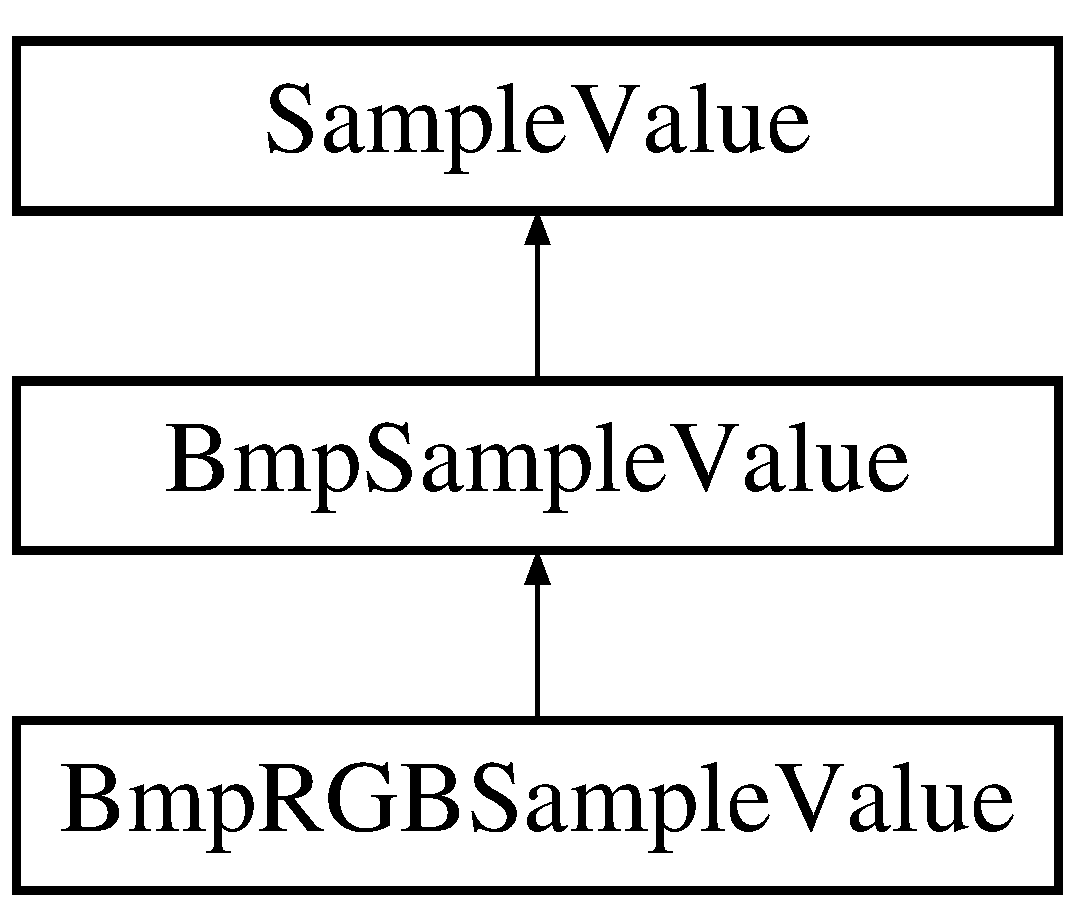
\includegraphics[height=3.000000cm]{classBmpRGBSampleValue}
\end{center}
\end{figure}
\subsection*{Public Member Functions}
\begin{DoxyCompactItemize}
\item 
\textbf{ Bmp\+R\+G\+B\+Sample\+Value} (\textbf{ B\+Y\+TE} r, \textbf{ B\+Y\+TE} g, \textbf{ B\+Y\+TE} b)
\item 
\textbf{ Bmp\+R\+G\+B\+Sample\+Value} (\textbf{ R\+G\+B\+Triple} t)
\item 
\textbf{ U\+W\+O\+R\+D32} \textbf{ calc\+Distance} (const \textbf{ Sample\+Value} $\ast$s) const
\item 
\textbf{ Sample\+Value} $\ast$ \textbf{ get\+Nearest\+Target\+Sample\+Value} (\textbf{ Emb\+Value} t) const
\item 
std\+::string \textbf{ get\+Name} (void) const
\item 
\textbf{ B\+Y\+TE} \textbf{ get\+Red} (void) const
\item 
\textbf{ B\+Y\+TE} \textbf{ get\+Green} (void) const
\item 
\textbf{ B\+Y\+TE} \textbf{ get\+Blue} (void) const
\end{DoxyCompactItemize}
\subsection*{Private Types}
\begin{DoxyCompactItemize}
\item 
enum \textbf{ C\+O\+L\+OR} \{ \textbf{ R\+ED}, 
\textbf{ G\+R\+E\+EN}, 
\textbf{ B\+L\+UE}
 \}
\item 
enum \textbf{ D\+I\+R\+E\+C\+T\+I\+ON} \{ \textbf{ UP}, 
\textbf{ D\+O\+WN}
 \}
\end{DoxyCompactItemize}
\subsection*{Private Member Functions}
\begin{DoxyCompactItemize}
\item 
\textbf{ U\+W\+O\+R\+D32} \textbf{ calc\+Key} (const \textbf{ R\+G\+B\+Triple} \&rgb) const
\item 
\textbf{ Emb\+Value} \textbf{ calc\+E\+Value} (const \textbf{ R\+G\+B\+Triple} \&rgb) const
\item 
\textbf{ B\+Y\+TE} \textbf{ plus} (\textbf{ B\+Y\+TE} a, \textbf{ B\+Y\+TE} b) const
\item 
\textbf{ B\+Y\+TE} \textbf{ minus} (\textbf{ B\+Y\+TE} a, \textbf{ B\+Y\+TE} b) const
\item 
void \textbf{ add\+N\+T\+S\+V\+Candidates} (std\+::vector$<$ \textbf{ R\+G\+B\+Triple} $>$ \&cands, const \textbf{ B\+Y\+TE} cube[3][2], \textbf{ C\+O\+L\+OR} fc, \textbf{ D\+I\+R\+E\+C\+T\+I\+ON} fd, \textbf{ C\+O\+L\+OR} i1, \textbf{ C\+O\+L\+OR} i2, \textbf{ Emb\+Value} t) const
\end{DoxyCompactItemize}
\subsection*{Private Attributes}
\begin{DoxyCompactItemize}
\item 
\textbf{ R\+G\+B\+Triple} \textbf{ Color}
\end{DoxyCompactItemize}
\subsection*{Additional Inherited Members}


\subsection{Member Enumeration Documentation}
\mbox{\label{classBmpRGBSampleValue_a1e5208b4f0d09c8f61d78cdfd5488d3d}} 
\index{Bmp\+R\+G\+B\+Sample\+Value@{Bmp\+R\+G\+B\+Sample\+Value}!C\+O\+L\+OR@{C\+O\+L\+OR}}
\index{C\+O\+L\+OR@{C\+O\+L\+OR}!Bmp\+R\+G\+B\+Sample\+Value@{Bmp\+R\+G\+B\+Sample\+Value}}
\subsubsection{C\+O\+L\+OR}
{\footnotesize\ttfamily enum \textbf{ Bmp\+R\+G\+B\+Sample\+Value\+::\+C\+O\+L\+OR}\hspace{0.3cm}{\ttfamily [private]}}

\begin{DoxyEnumFields}{Enumerator}
\raisebox{\heightof{T}}[0pt][0pt]{\index{R\+ED@{R\+ED}!Bmp\+R\+G\+B\+Sample\+Value@{Bmp\+R\+G\+B\+Sample\+Value}}\index{Bmp\+R\+G\+B\+Sample\+Value@{Bmp\+R\+G\+B\+Sample\+Value}!R\+ED@{R\+ED}}}\mbox{\label{classBmpRGBSampleValue_a1e5208b4f0d09c8f61d78cdfd5488d3da4d2386856b553e3831419719cf284704}} 
R\+ED&\\
\hline

\raisebox{\heightof{T}}[0pt][0pt]{\index{G\+R\+E\+EN@{G\+R\+E\+EN}!Bmp\+R\+G\+B\+Sample\+Value@{Bmp\+R\+G\+B\+Sample\+Value}}\index{Bmp\+R\+G\+B\+Sample\+Value@{Bmp\+R\+G\+B\+Sample\+Value}!G\+R\+E\+EN@{G\+R\+E\+EN}}}\mbox{\label{classBmpRGBSampleValue_a1e5208b4f0d09c8f61d78cdfd5488d3da1c65467ddf0f5d047a09cb2e772e1140}} 
G\+R\+E\+EN&\\
\hline

\raisebox{\heightof{T}}[0pt][0pt]{\index{B\+L\+UE@{B\+L\+UE}!Bmp\+R\+G\+B\+Sample\+Value@{Bmp\+R\+G\+B\+Sample\+Value}}\index{Bmp\+R\+G\+B\+Sample\+Value@{Bmp\+R\+G\+B\+Sample\+Value}!B\+L\+UE@{B\+L\+UE}}}\mbox{\label{classBmpRGBSampleValue_a1e5208b4f0d09c8f61d78cdfd5488d3da4f80e6362ff5d7e0e27950d7d18ca7de}} 
B\+L\+UE&\\
\hline

\end{DoxyEnumFields}
\mbox{\label{classBmpRGBSampleValue_ac0d93f8972ad38b753b94df6991f77f6}} 
\index{Bmp\+R\+G\+B\+Sample\+Value@{Bmp\+R\+G\+B\+Sample\+Value}!D\+I\+R\+E\+C\+T\+I\+ON@{D\+I\+R\+E\+C\+T\+I\+ON}}
\index{D\+I\+R\+E\+C\+T\+I\+ON@{D\+I\+R\+E\+C\+T\+I\+ON}!Bmp\+R\+G\+B\+Sample\+Value@{Bmp\+R\+G\+B\+Sample\+Value}}
\subsubsection{D\+I\+R\+E\+C\+T\+I\+ON}
{\footnotesize\ttfamily enum \textbf{ Bmp\+R\+G\+B\+Sample\+Value\+::\+D\+I\+R\+E\+C\+T\+I\+ON}\hspace{0.3cm}{\ttfamily [private]}}

\begin{DoxyEnumFields}{Enumerator}
\raisebox{\heightof{T}}[0pt][0pt]{\index{UP@{UP}!Bmp\+R\+G\+B\+Sample\+Value@{Bmp\+R\+G\+B\+Sample\+Value}}\index{Bmp\+R\+G\+B\+Sample\+Value@{Bmp\+R\+G\+B\+Sample\+Value}!UP@{UP}}}\mbox{\label{classBmpRGBSampleValue_ac0d93f8972ad38b753b94df6991f77f6ac51fc636bcbf6661c93467e2e7ca2130}} 
UP&\\
\hline

\raisebox{\heightof{T}}[0pt][0pt]{\index{D\+O\+WN@{D\+O\+WN}!Bmp\+R\+G\+B\+Sample\+Value@{Bmp\+R\+G\+B\+Sample\+Value}}\index{Bmp\+R\+G\+B\+Sample\+Value@{Bmp\+R\+G\+B\+Sample\+Value}!D\+O\+WN@{D\+O\+WN}}}\mbox{\label{classBmpRGBSampleValue_ac0d93f8972ad38b753b94df6991f77f6a0a44fea06b72341ea0b8c0984d2ed71b}} 
D\+O\+WN&\\
\hline

\end{DoxyEnumFields}


\subsection{Constructor \& Destructor Documentation}
\mbox{\label{classBmpRGBSampleValue_a2038cd4fa8aa78195078db8a40e8af50}} 
\index{Bmp\+R\+G\+B\+Sample\+Value@{Bmp\+R\+G\+B\+Sample\+Value}!Bmp\+R\+G\+B\+Sample\+Value@{Bmp\+R\+G\+B\+Sample\+Value}}
\index{Bmp\+R\+G\+B\+Sample\+Value@{Bmp\+R\+G\+B\+Sample\+Value}!Bmp\+R\+G\+B\+Sample\+Value@{Bmp\+R\+G\+B\+Sample\+Value}}
\subsubsection{Bmp\+R\+G\+B\+Sample\+Value()\hspace{0.1cm}{\footnotesize\ttfamily [1/2]}}
{\footnotesize\ttfamily Bmp\+R\+G\+B\+Sample\+Value\+::\+Bmp\+R\+G\+B\+Sample\+Value (\begin{DoxyParamCaption}\item[{\textbf{ B\+Y\+TE}}]{r,  }\item[{\textbf{ B\+Y\+TE}}]{g,  }\item[{\textbf{ B\+Y\+TE}}]{b }\end{DoxyParamCaption})}

\mbox{\label{classBmpRGBSampleValue_a0b9ae2be392fe5f69f8e44fa1ac281af}} 
\index{Bmp\+R\+G\+B\+Sample\+Value@{Bmp\+R\+G\+B\+Sample\+Value}!Bmp\+R\+G\+B\+Sample\+Value@{Bmp\+R\+G\+B\+Sample\+Value}}
\index{Bmp\+R\+G\+B\+Sample\+Value@{Bmp\+R\+G\+B\+Sample\+Value}!Bmp\+R\+G\+B\+Sample\+Value@{Bmp\+R\+G\+B\+Sample\+Value}}
\subsubsection{Bmp\+R\+G\+B\+Sample\+Value()\hspace{0.1cm}{\footnotesize\ttfamily [2/2]}}
{\footnotesize\ttfamily Bmp\+R\+G\+B\+Sample\+Value\+::\+Bmp\+R\+G\+B\+Sample\+Value (\begin{DoxyParamCaption}\item[{\textbf{ R\+G\+B\+Triple}}]{t }\end{DoxyParamCaption})}



\subsection{Member Function Documentation}
\mbox{\label{classBmpRGBSampleValue_a8ab93cbcaea74c8fb1dd724316d5706c}} 
\index{Bmp\+R\+G\+B\+Sample\+Value@{Bmp\+R\+G\+B\+Sample\+Value}!add\+N\+T\+S\+V\+Candidates@{add\+N\+T\+S\+V\+Candidates}}
\index{add\+N\+T\+S\+V\+Candidates@{add\+N\+T\+S\+V\+Candidates}!Bmp\+R\+G\+B\+Sample\+Value@{Bmp\+R\+G\+B\+Sample\+Value}}
\subsubsection{add\+N\+T\+S\+V\+Candidates()}
{\footnotesize\ttfamily void Bmp\+R\+G\+B\+Sample\+Value\+::add\+N\+T\+S\+V\+Candidates (\begin{DoxyParamCaption}\item[{std\+::vector$<$ \textbf{ R\+G\+B\+Triple} $>$ \&}]{cands,  }\item[{const \textbf{ B\+Y\+TE}}]{cube[3][2],  }\item[{\textbf{ C\+O\+L\+OR}}]{fc,  }\item[{\textbf{ D\+I\+R\+E\+C\+T\+I\+ON}}]{fd,  }\item[{\textbf{ C\+O\+L\+OR}}]{i1,  }\item[{\textbf{ C\+O\+L\+OR}}]{i2,  }\item[{\textbf{ Emb\+Value}}]{t }\end{DoxyParamCaption}) const\hspace{0.3cm}{\ttfamily [private]}}

add candidates for the nearest target sample value 
\begin{DoxyParams}{Parameters}
{\em cands} & the candidates vector \\
\hline
{\em cube} & the color values describing the current search cube \\
\hline
{\em fc} & the fixed color \\
\hline
{\em fd} & the fixed side of the fixed color \\
\hline
\end{DoxyParams}
\mbox{\label{classBmpRGBSampleValue_a41c765b2108e640d3e7249f5dfd81eef}} 
\index{Bmp\+R\+G\+B\+Sample\+Value@{Bmp\+R\+G\+B\+Sample\+Value}!calc\+Distance@{calc\+Distance}}
\index{calc\+Distance@{calc\+Distance}!Bmp\+R\+G\+B\+Sample\+Value@{Bmp\+R\+G\+B\+Sample\+Value}}
\subsubsection{calc\+Distance()}
{\footnotesize\ttfamily \textbf{ U\+W\+O\+R\+D32} Bmp\+R\+G\+B\+Sample\+Value\+::calc\+Distance (\begin{DoxyParamCaption}\item[{const \textbf{ Sample\+Value} $\ast$}]{s }\end{DoxyParamCaption}) const\hspace{0.3cm}{\ttfamily [virtual]}}

calculate the distance between the sample value s and this sample value 
\begin{DoxyParams}{Parameters}
{\em s} & a sample value of the same type as this \\
\hline
\end{DoxyParams}
\begin{DoxyReturn}{Returns}
the distance 
\end{DoxyReturn}


Reimplemented from \textbf{ Bmp\+Sample\+Value} \doxyref{}{p.}{classBmpSampleValue_af81c03b48ec98543a9e1a88b69b83abd}.

\mbox{\label{classBmpRGBSampleValue_ac12516b1fc1bc05f277150efe4c65153}} 
\index{Bmp\+R\+G\+B\+Sample\+Value@{Bmp\+R\+G\+B\+Sample\+Value}!calc\+E\+Value@{calc\+E\+Value}}
\index{calc\+E\+Value@{calc\+E\+Value}!Bmp\+R\+G\+B\+Sample\+Value@{Bmp\+R\+G\+B\+Sample\+Value}}
\subsubsection{calc\+E\+Value()}
{\footnotesize\ttfamily \textbf{ Emb\+Value} Bmp\+R\+G\+B\+Sample\+Value\+::calc\+E\+Value (\begin{DoxyParamCaption}\item[{const \textbf{ R\+G\+B\+Triple} \&}]{rgb }\end{DoxyParamCaption}) const\hspace{0.3cm}{\ttfamily [inline]}, {\ttfamily [private]}}

\mbox{\label{classBmpRGBSampleValue_aed6e7619877620050d4a7bd388c4b29e}} 
\index{Bmp\+R\+G\+B\+Sample\+Value@{Bmp\+R\+G\+B\+Sample\+Value}!calc\+Key@{calc\+Key}}
\index{calc\+Key@{calc\+Key}!Bmp\+R\+G\+B\+Sample\+Value@{Bmp\+R\+G\+B\+Sample\+Value}}
\subsubsection{calc\+Key()}
{\footnotesize\ttfamily \textbf{ U\+W\+O\+R\+D32} Bmp\+R\+G\+B\+Sample\+Value\+::calc\+Key (\begin{DoxyParamCaption}\item[{const \textbf{ R\+G\+B\+Triple} \&}]{rgb }\end{DoxyParamCaption}) const\hspace{0.3cm}{\ttfamily [inline]}, {\ttfamily [private]}}

\mbox{\label{classBmpRGBSampleValue_a35de04de107bf2a1f66f53eac3ab2b8d}} 
\index{Bmp\+R\+G\+B\+Sample\+Value@{Bmp\+R\+G\+B\+Sample\+Value}!get\+Blue@{get\+Blue}}
\index{get\+Blue@{get\+Blue}!Bmp\+R\+G\+B\+Sample\+Value@{Bmp\+R\+G\+B\+Sample\+Value}}
\subsubsection{get\+Blue()}
{\footnotesize\ttfamily \textbf{ B\+Y\+TE} Bmp\+R\+G\+B\+Sample\+Value\+::get\+Blue (\begin{DoxyParamCaption}\item[{void}]{ }\end{DoxyParamCaption}) const\hspace{0.3cm}{\ttfamily [inline]}, {\ttfamily [virtual]}}

get the blue color component 

Implements \textbf{ Bmp\+Sample\+Value} \doxyref{}{p.}{classBmpSampleValue_a0c31d4428158c7c6017935ac03254b26}.

\mbox{\label{classBmpRGBSampleValue_a9c1418294f6552b218a05a2439ee5df0}} 
\index{Bmp\+R\+G\+B\+Sample\+Value@{Bmp\+R\+G\+B\+Sample\+Value}!get\+Green@{get\+Green}}
\index{get\+Green@{get\+Green}!Bmp\+R\+G\+B\+Sample\+Value@{Bmp\+R\+G\+B\+Sample\+Value}}
\subsubsection{get\+Green()}
{\footnotesize\ttfamily \textbf{ B\+Y\+TE} Bmp\+R\+G\+B\+Sample\+Value\+::get\+Green (\begin{DoxyParamCaption}\item[{void}]{ }\end{DoxyParamCaption}) const\hspace{0.3cm}{\ttfamily [inline]}, {\ttfamily [virtual]}}

get the green color component 

Implements \textbf{ Bmp\+Sample\+Value} \doxyref{}{p.}{classBmpSampleValue_a5d646a4082648a5b63323167553066ab}.

\mbox{\label{classBmpRGBSampleValue_a4937eb190ebfedbd7b97b899e15855db}} 
\index{Bmp\+R\+G\+B\+Sample\+Value@{Bmp\+R\+G\+B\+Sample\+Value}!get\+Name@{get\+Name}}
\index{get\+Name@{get\+Name}!Bmp\+R\+G\+B\+Sample\+Value@{Bmp\+R\+G\+B\+Sample\+Value}}
\subsubsection{get\+Name()}
{\footnotesize\ttfamily std\+::string Bmp\+R\+G\+B\+Sample\+Value\+::get\+Name (\begin{DoxyParamCaption}\item[{void}]{ }\end{DoxyParamCaption}) const\hspace{0.3cm}{\ttfamily [virtual]}}

return a short name uniquely identifying this sample value 

Implements \textbf{ Sample\+Value} \doxyref{}{p.}{classSampleValue_aeaf5c46ec6d023840e9773604b20d25c}.

\mbox{\label{classBmpRGBSampleValue_a8dcb01b4e05109a5ddabf882b4bb3b41}} 
\index{Bmp\+R\+G\+B\+Sample\+Value@{Bmp\+R\+G\+B\+Sample\+Value}!get\+Nearest\+Target\+Sample\+Value@{get\+Nearest\+Target\+Sample\+Value}}
\index{get\+Nearest\+Target\+Sample\+Value@{get\+Nearest\+Target\+Sample\+Value}!Bmp\+R\+G\+B\+Sample\+Value@{Bmp\+R\+G\+B\+Sample\+Value}}
\subsubsection{get\+Nearest\+Target\+Sample\+Value()}
{\footnotesize\ttfamily \textbf{ Sample\+Value} $\ast$ Bmp\+R\+G\+B\+Sample\+Value\+::get\+Nearest\+Target\+Sample\+Value (\begin{DoxyParamCaption}\item[{\textbf{ Emb\+Value}}]{t }\end{DoxyParamCaption}) const\hspace{0.3cm}{\ttfamily [virtual]}}

get the nearest (with the least distance to this sample value) sample value whose embedded value equals the specified target 
\begin{DoxyParams}{Parameters}
{\em t} & the target embedded value\\
\hline
\end{DoxyParams}
If two or more target sample values have equal distance each of them should be returned with equal probability.

The returned \doxyref{Sample\+Value}{p.}{classSampleValue} object should be deleted by the callser. 

Implements \textbf{ Sample\+Value} \doxyref{}{p.}{classSampleValue_aeca3fc1fd34c09d2244706b010935c2c}.

\mbox{\label{classBmpRGBSampleValue_a8cbb5d220b2be0d1b9239d7abcda3a55}} 
\index{Bmp\+R\+G\+B\+Sample\+Value@{Bmp\+R\+G\+B\+Sample\+Value}!get\+Red@{get\+Red}}
\index{get\+Red@{get\+Red}!Bmp\+R\+G\+B\+Sample\+Value@{Bmp\+R\+G\+B\+Sample\+Value}}
\subsubsection{get\+Red()}
{\footnotesize\ttfamily \textbf{ B\+Y\+TE} Bmp\+R\+G\+B\+Sample\+Value\+::get\+Red (\begin{DoxyParamCaption}\item[{void}]{ }\end{DoxyParamCaption}) const\hspace{0.3cm}{\ttfamily [inline]}, {\ttfamily [virtual]}}

get the red color component 

Implements \textbf{ Bmp\+Sample\+Value} \doxyref{}{p.}{classBmpSampleValue_a8665a4c4db9ac910abf4ec0738cfde68}.

\mbox{\label{classBmpRGBSampleValue_ad2e6b7d9a3b37936732d63dc268f833b}} 
\index{Bmp\+R\+G\+B\+Sample\+Value@{Bmp\+R\+G\+B\+Sample\+Value}!minus@{minus}}
\index{minus@{minus}!Bmp\+R\+G\+B\+Sample\+Value@{Bmp\+R\+G\+B\+Sample\+Value}}
\subsubsection{minus()}
{\footnotesize\ttfamily \textbf{ B\+Y\+TE} Bmp\+R\+G\+B\+Sample\+Value\+::minus (\begin{DoxyParamCaption}\item[{\textbf{ B\+Y\+TE}}]{a,  }\item[{\textbf{ B\+Y\+TE}}]{b }\end{DoxyParamCaption}) const\hspace{0.3cm}{\ttfamily [private]}}

substract the B\+Y\+TE b from the B\+Y\+TE a \begin{DoxyReturn}{Returns}
max(0, a -\/ b) 
\end{DoxyReturn}
\mbox{\label{classBmpRGBSampleValue_a54f1b405be7151da0b955402b0673e71}} 
\index{Bmp\+R\+G\+B\+Sample\+Value@{Bmp\+R\+G\+B\+Sample\+Value}!plus@{plus}}
\index{plus@{plus}!Bmp\+R\+G\+B\+Sample\+Value@{Bmp\+R\+G\+B\+Sample\+Value}}
\subsubsection{plus()}
{\footnotesize\ttfamily \textbf{ B\+Y\+TE} Bmp\+R\+G\+B\+Sample\+Value\+::plus (\begin{DoxyParamCaption}\item[{\textbf{ B\+Y\+TE}}]{a,  }\item[{\textbf{ B\+Y\+TE}}]{b }\end{DoxyParamCaption}) const\hspace{0.3cm}{\ttfamily [private]}}

add the B\+Y\+T\+Es a and b \begin{DoxyReturn}{Returns}
min(255, a + b) 
\end{DoxyReturn}


\subsection{Member Data Documentation}
\mbox{\label{classBmpRGBSampleValue_a48f3be8e29c6e6689a7e8456fe298c3f}} 
\index{Bmp\+R\+G\+B\+Sample\+Value@{Bmp\+R\+G\+B\+Sample\+Value}!Color@{Color}}
\index{Color@{Color}!Bmp\+R\+G\+B\+Sample\+Value@{Bmp\+R\+G\+B\+Sample\+Value}}
\subsubsection{Color}
{\footnotesize\ttfamily \textbf{ R\+G\+B\+Triple} Bmp\+R\+G\+B\+Sample\+Value\+::\+Color\hspace{0.3cm}{\ttfamily [private]}}



The documentation for this class was generated from the following files\+:\begin{DoxyCompactItemize}
\item 
\textbf{ Bmp\+R\+G\+B\+Sample\+Value.\+h}\item 
\textbf{ Bmp\+R\+G\+B\+Sample\+Value.\+cc}\end{DoxyCompactItemize}

\section{Bmp\+R\+G\+B\+Sample\+Value\+Test Class Reference}
\label{classBmpRGBSampleValueTest}\index{Bmp\+R\+G\+B\+Sample\+Value\+Test@{Bmp\+R\+G\+B\+Sample\+Value\+Test}}


{\ttfamily \#include $<$Bmp\+R\+G\+B\+Sample\+Value\+Test.\+h$>$}

Inheritance diagram for Bmp\+R\+G\+B\+Sample\+Value\+Test\+:\begin{figure}[H]
\begin{center}
\leavevmode
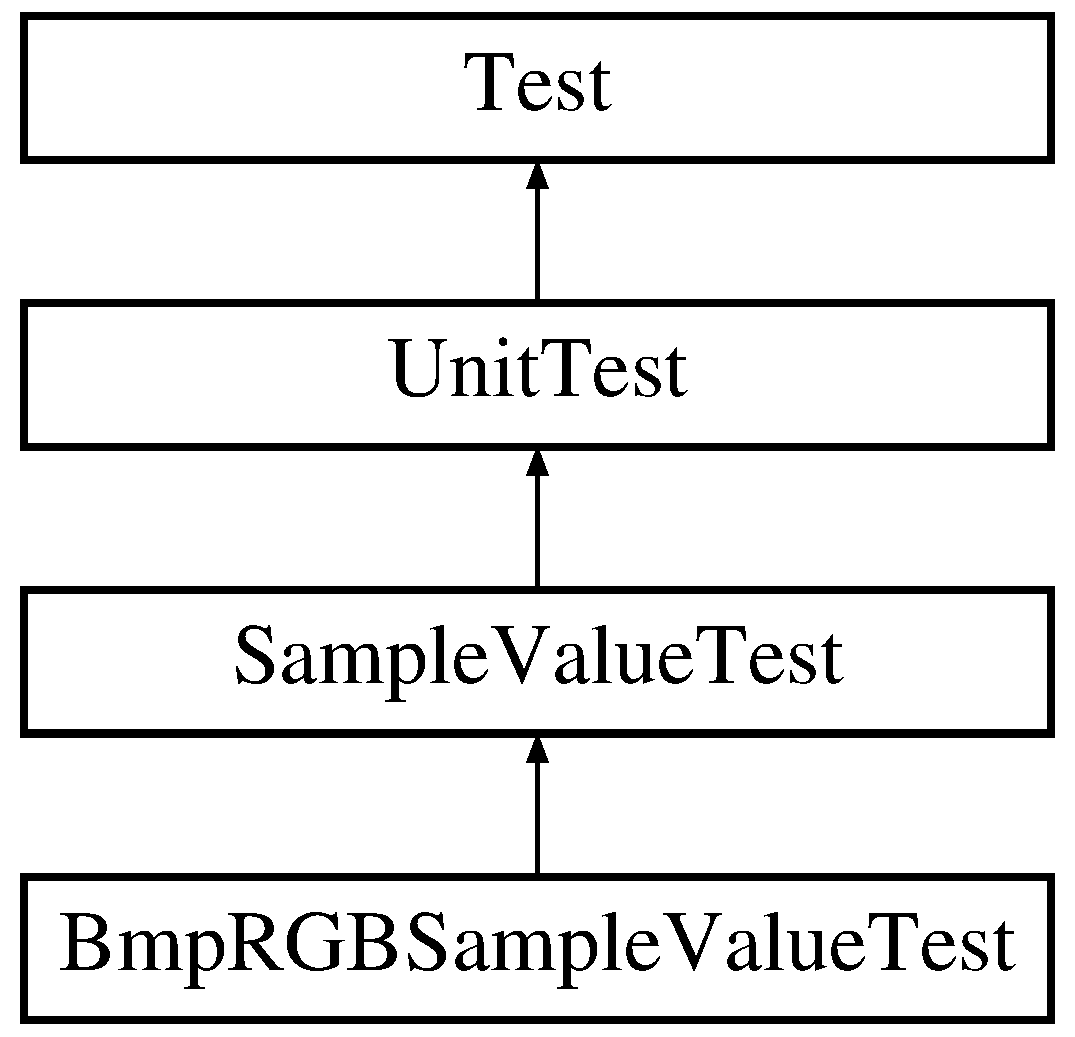
\includegraphics[height=4.000000cm]{classBmpRGBSampleValueTest}
\end{center}
\end{figure}
\subsection*{Public Member Functions}
\begin{DoxyCompactItemize}
\item 
\textbf{ Bmp\+R\+G\+B\+Sample\+Value\+Test} (\textbf{ Test\+Suite} $\ast$s)
\item 
void \textbf{ setup} (void)
\item 
void \textbf{ cleanup} (void)
\item 
void \textbf{ test\+Distance} (void)
\item 
void \textbf{ test\+Is\+Neighbour} (void)
\end{DoxyCompactItemize}
\subsection*{Private Attributes}
\begin{DoxyCompactItemize}
\item 
\textbf{ Cvr\+Stg\+File} $\ast$ \textbf{ f\+\_\+win}
\item 
\textbf{ Cvr\+Stg\+File} $\ast$ \textbf{ f\+\_\+os2}
\item 
\textbf{ Sample\+Value} $\ast$ \textbf{ sv\+\_\+0\+\_\+0\+\_\+0}
\item 
\textbf{ Sample\+Value} $\ast$ \textbf{ sv\+\_\+1\+\_\+1\+\_\+1}
\item 
\textbf{ Sample\+Value} $\ast$ \textbf{ sv\+\_\+0\+\_\+3\+\_\+4}
\item 
\textbf{ Sample\+Value} $\ast$ \textbf{ sv\+\_\+10\+\_\+10\+\_\+10}
\item 
\textbf{ Sample\+Value} $\ast$ \textbf{ sv\+\_\+12\+\_\+13\+\_\+14}
\item 
\textbf{ Sample\+Value} $\ast$ \textbf{ sv\+\_\+128\+\_\+128\+\_\+128}
\item 
\textbf{ Sample\+Value} $\ast$ \textbf{ sv\+\_\+210\+\_\+0\+\_\+120}
\item 
\textbf{ Sample\+Value} $\ast$ \textbf{ sv\+\_\+255\+\_\+255\+\_\+255}
\item 
\textbf{ Globals} \textbf{ gl\+\_\+win}
\item 
\textbf{ Globals} \textbf{ gl\+\_\+os2}
\end{DoxyCompactItemize}
\subsection*{Additional Inherited Members}


\subsection{Constructor \& Destructor Documentation}
\mbox{\label{classBmpRGBSampleValueTest_a3d4f46591983b54f41ec0fcc12da8972}} 
\index{Bmp\+R\+G\+B\+Sample\+Value\+Test@{Bmp\+R\+G\+B\+Sample\+Value\+Test}!Bmp\+R\+G\+B\+Sample\+Value\+Test@{Bmp\+R\+G\+B\+Sample\+Value\+Test}}
\index{Bmp\+R\+G\+B\+Sample\+Value\+Test@{Bmp\+R\+G\+B\+Sample\+Value\+Test}!Bmp\+R\+G\+B\+Sample\+Value\+Test@{Bmp\+R\+G\+B\+Sample\+Value\+Test}}
\subsubsection{Bmp\+R\+G\+B\+Sample\+Value\+Test()}
{\footnotesize\ttfamily Bmp\+R\+G\+B\+Sample\+Value\+Test\+::\+Bmp\+R\+G\+B\+Sample\+Value\+Test (\begin{DoxyParamCaption}\item[{\textbf{ Test\+Suite} $\ast$}]{s }\end{DoxyParamCaption})}



\subsection{Member Function Documentation}
\mbox{\label{classBmpRGBSampleValueTest_a678eb59000fdb188caf33fd5bb3c8ca2}} 
\index{Bmp\+R\+G\+B\+Sample\+Value\+Test@{Bmp\+R\+G\+B\+Sample\+Value\+Test}!cleanup@{cleanup}}
\index{cleanup@{cleanup}!Bmp\+R\+G\+B\+Sample\+Value\+Test@{Bmp\+R\+G\+B\+Sample\+Value\+Test}}
\subsubsection{cleanup()}
{\footnotesize\ttfamily void Bmp\+R\+G\+B\+Sample\+Value\+Test\+::cleanup (\begin{DoxyParamCaption}\item[{void}]{ }\end{DoxyParamCaption})\hspace{0.3cm}{\ttfamily [virtual]}}

cleanup the unit test -\/ called after run 

Reimplemented from \textbf{ Unit\+Test} \doxyref{}{p.}{classUnitTest_adf77efe972ee4a766d94e3f7ddc193ad}.

\mbox{\label{classBmpRGBSampleValueTest_a55f098ab9be37a93fa7a88bd6f71f097}} 
\index{Bmp\+R\+G\+B\+Sample\+Value\+Test@{Bmp\+R\+G\+B\+Sample\+Value\+Test}!setup@{setup}}
\index{setup@{setup}!Bmp\+R\+G\+B\+Sample\+Value\+Test@{Bmp\+R\+G\+B\+Sample\+Value\+Test}}
\subsubsection{setup()}
{\footnotesize\ttfamily void Bmp\+R\+G\+B\+Sample\+Value\+Test\+::setup (\begin{DoxyParamCaption}\item[{void}]{ }\end{DoxyParamCaption})\hspace{0.3cm}{\ttfamily [virtual]}}

setup the unit test -\/ called before run

\doxyref{Unit\+Test\+::setup}{p.}{classUnitTest_ad73fdf9012b651047ea001d21f9d27ad} will (together with \doxyref{Unit\+Test\+::cleanup}{p.}{classUnitTest_adf77efe972ee4a766d94e3f7ddc193ad}) save and restore the object stored in Globs so they should be called from the corresponding functions in the derived object if the derived unit test manipulates the Globs object. 

Reimplemented from \textbf{ Unit\+Test} \doxyref{}{p.}{classUnitTest_ad73fdf9012b651047ea001d21f9d27ad}.

\mbox{\label{classBmpRGBSampleValueTest_ad74a7791b77dda35fe0f40f132f78cd6}} 
\index{Bmp\+R\+G\+B\+Sample\+Value\+Test@{Bmp\+R\+G\+B\+Sample\+Value\+Test}!test\+Distance@{test\+Distance}}
\index{test\+Distance@{test\+Distance}!Bmp\+R\+G\+B\+Sample\+Value\+Test@{Bmp\+R\+G\+B\+Sample\+Value\+Test}}
\subsubsection{test\+Distance()}
{\footnotesize\ttfamily void Bmp\+R\+G\+B\+Sample\+Value\+Test\+::test\+Distance (\begin{DoxyParamCaption}\item[{void}]{ }\end{DoxyParamCaption})}

\mbox{\label{classBmpRGBSampleValueTest_a6b3aa9238b1b79358982b0027e3bbe8a}} 
\index{Bmp\+R\+G\+B\+Sample\+Value\+Test@{Bmp\+R\+G\+B\+Sample\+Value\+Test}!test\+Is\+Neighbour@{test\+Is\+Neighbour}}
\index{test\+Is\+Neighbour@{test\+Is\+Neighbour}!Bmp\+R\+G\+B\+Sample\+Value\+Test@{Bmp\+R\+G\+B\+Sample\+Value\+Test}}
\subsubsection{test\+Is\+Neighbour()}
{\footnotesize\ttfamily void Bmp\+R\+G\+B\+Sample\+Value\+Test\+::test\+Is\+Neighbour (\begin{DoxyParamCaption}\item[{void}]{ }\end{DoxyParamCaption})}



\subsection{Member Data Documentation}
\mbox{\label{classBmpRGBSampleValueTest_ac59d97c111e97b83bf37751f3f024307}} 
\index{Bmp\+R\+G\+B\+Sample\+Value\+Test@{Bmp\+R\+G\+B\+Sample\+Value\+Test}!f\+\_\+os2@{f\+\_\+os2}}
\index{f\+\_\+os2@{f\+\_\+os2}!Bmp\+R\+G\+B\+Sample\+Value\+Test@{Bmp\+R\+G\+B\+Sample\+Value\+Test}}
\subsubsection{f\+\_\+os2}
{\footnotesize\ttfamily \textbf{ Cvr\+Stg\+File} $\ast$ Bmp\+R\+G\+B\+Sample\+Value\+Test\+::f\+\_\+os2\hspace{0.3cm}{\ttfamily [private]}}

\mbox{\label{classBmpRGBSampleValueTest_a9746845f4999eb45073f0cef513b4e05}} 
\index{Bmp\+R\+G\+B\+Sample\+Value\+Test@{Bmp\+R\+G\+B\+Sample\+Value\+Test}!f\+\_\+win@{f\+\_\+win}}
\index{f\+\_\+win@{f\+\_\+win}!Bmp\+R\+G\+B\+Sample\+Value\+Test@{Bmp\+R\+G\+B\+Sample\+Value\+Test}}
\subsubsection{f\+\_\+win}
{\footnotesize\ttfamily \textbf{ Cvr\+Stg\+File}$\ast$ Bmp\+R\+G\+B\+Sample\+Value\+Test\+::f\+\_\+win\hspace{0.3cm}{\ttfamily [private]}}

\mbox{\label{classBmpRGBSampleValueTest_a16fa18f2a3c29fefeb7397cbf2a869da}} 
\index{Bmp\+R\+G\+B\+Sample\+Value\+Test@{Bmp\+R\+G\+B\+Sample\+Value\+Test}!gl\+\_\+os2@{gl\+\_\+os2}}
\index{gl\+\_\+os2@{gl\+\_\+os2}!Bmp\+R\+G\+B\+Sample\+Value\+Test@{Bmp\+R\+G\+B\+Sample\+Value\+Test}}
\subsubsection{gl\+\_\+os2}
{\footnotesize\ttfamily \textbf{ Globals} Bmp\+R\+G\+B\+Sample\+Value\+Test\+::gl\+\_\+os2\hspace{0.3cm}{\ttfamily [private]}}

\mbox{\label{classBmpRGBSampleValueTest_aa233f17c5cf4d09cd191fa80366f8653}} 
\index{Bmp\+R\+G\+B\+Sample\+Value\+Test@{Bmp\+R\+G\+B\+Sample\+Value\+Test}!gl\+\_\+win@{gl\+\_\+win}}
\index{gl\+\_\+win@{gl\+\_\+win}!Bmp\+R\+G\+B\+Sample\+Value\+Test@{Bmp\+R\+G\+B\+Sample\+Value\+Test}}
\subsubsection{gl\+\_\+win}
{\footnotesize\ttfamily \textbf{ Globals} Bmp\+R\+G\+B\+Sample\+Value\+Test\+::gl\+\_\+win\hspace{0.3cm}{\ttfamily [private]}}

\mbox{\label{classBmpRGBSampleValueTest_a3aaa104bfd6a9bf6aae468167e522a65}} 
\index{Bmp\+R\+G\+B\+Sample\+Value\+Test@{Bmp\+R\+G\+B\+Sample\+Value\+Test}!sv\+\_\+0\+\_\+0\+\_\+0@{sv\+\_\+0\+\_\+0\+\_\+0}}
\index{sv\+\_\+0\+\_\+0\+\_\+0@{sv\+\_\+0\+\_\+0\+\_\+0}!Bmp\+R\+G\+B\+Sample\+Value\+Test@{Bmp\+R\+G\+B\+Sample\+Value\+Test}}
\subsubsection{sv\+\_\+0\+\_\+0\+\_\+0}
{\footnotesize\ttfamily \textbf{ Sample\+Value}$\ast$ Bmp\+R\+G\+B\+Sample\+Value\+Test\+::sv\+\_\+0\+\_\+0\+\_\+0\hspace{0.3cm}{\ttfamily [private]}}

\mbox{\label{classBmpRGBSampleValueTest_a3e477edba31ced22d10d4d2000695c9a}} 
\index{Bmp\+R\+G\+B\+Sample\+Value\+Test@{Bmp\+R\+G\+B\+Sample\+Value\+Test}!sv\+\_\+0\+\_\+3\+\_\+4@{sv\+\_\+0\+\_\+3\+\_\+4}}
\index{sv\+\_\+0\+\_\+3\+\_\+4@{sv\+\_\+0\+\_\+3\+\_\+4}!Bmp\+R\+G\+B\+Sample\+Value\+Test@{Bmp\+R\+G\+B\+Sample\+Value\+Test}}
\subsubsection{sv\+\_\+0\+\_\+3\+\_\+4}
{\footnotesize\ttfamily \textbf{ Sample\+Value} $\ast$ Bmp\+R\+G\+B\+Sample\+Value\+Test\+::sv\+\_\+0\+\_\+3\+\_\+4\hspace{0.3cm}{\ttfamily [private]}}

\mbox{\label{classBmpRGBSampleValueTest_af9541467702aca247fad6b13f050a7e1}} 
\index{Bmp\+R\+G\+B\+Sample\+Value\+Test@{Bmp\+R\+G\+B\+Sample\+Value\+Test}!sv\+\_\+10\+\_\+10\+\_\+10@{sv\+\_\+10\+\_\+10\+\_\+10}}
\index{sv\+\_\+10\+\_\+10\+\_\+10@{sv\+\_\+10\+\_\+10\+\_\+10}!Bmp\+R\+G\+B\+Sample\+Value\+Test@{Bmp\+R\+G\+B\+Sample\+Value\+Test}}
\subsubsection{sv\+\_\+10\+\_\+10\+\_\+10}
{\footnotesize\ttfamily \textbf{ Sample\+Value} $\ast$ Bmp\+R\+G\+B\+Sample\+Value\+Test\+::sv\+\_\+10\+\_\+10\+\_\+10\hspace{0.3cm}{\ttfamily [private]}}

\mbox{\label{classBmpRGBSampleValueTest_ab39be9400b2f34c2bfecf77ceda4381c}} 
\index{Bmp\+R\+G\+B\+Sample\+Value\+Test@{Bmp\+R\+G\+B\+Sample\+Value\+Test}!sv\+\_\+128\+\_\+128\+\_\+128@{sv\+\_\+128\+\_\+128\+\_\+128}}
\index{sv\+\_\+128\+\_\+128\+\_\+128@{sv\+\_\+128\+\_\+128\+\_\+128}!Bmp\+R\+G\+B\+Sample\+Value\+Test@{Bmp\+R\+G\+B\+Sample\+Value\+Test}}
\subsubsection{sv\+\_\+128\+\_\+128\+\_\+128}
{\footnotesize\ttfamily \textbf{ Sample\+Value} $\ast$ Bmp\+R\+G\+B\+Sample\+Value\+Test\+::sv\+\_\+128\+\_\+128\+\_\+128\hspace{0.3cm}{\ttfamily [private]}}

\mbox{\label{classBmpRGBSampleValueTest_a5957164aebb4b04a557bfe23003697cf}} 
\index{Bmp\+R\+G\+B\+Sample\+Value\+Test@{Bmp\+R\+G\+B\+Sample\+Value\+Test}!sv\+\_\+12\+\_\+13\+\_\+14@{sv\+\_\+12\+\_\+13\+\_\+14}}
\index{sv\+\_\+12\+\_\+13\+\_\+14@{sv\+\_\+12\+\_\+13\+\_\+14}!Bmp\+R\+G\+B\+Sample\+Value\+Test@{Bmp\+R\+G\+B\+Sample\+Value\+Test}}
\subsubsection{sv\+\_\+12\+\_\+13\+\_\+14}
{\footnotesize\ttfamily \textbf{ Sample\+Value} $\ast$ Bmp\+R\+G\+B\+Sample\+Value\+Test\+::sv\+\_\+12\+\_\+13\+\_\+14\hspace{0.3cm}{\ttfamily [private]}}

\mbox{\label{classBmpRGBSampleValueTest_a9d0c3f0fc9ac1f5923bdd75dd308c499}} 
\index{Bmp\+R\+G\+B\+Sample\+Value\+Test@{Bmp\+R\+G\+B\+Sample\+Value\+Test}!sv\+\_\+1\+\_\+1\+\_\+1@{sv\+\_\+1\+\_\+1\+\_\+1}}
\index{sv\+\_\+1\+\_\+1\+\_\+1@{sv\+\_\+1\+\_\+1\+\_\+1}!Bmp\+R\+G\+B\+Sample\+Value\+Test@{Bmp\+R\+G\+B\+Sample\+Value\+Test}}
\subsubsection{sv\+\_\+1\+\_\+1\+\_\+1}
{\footnotesize\ttfamily \textbf{ Sample\+Value} $\ast$ Bmp\+R\+G\+B\+Sample\+Value\+Test\+::sv\+\_\+1\+\_\+1\+\_\+1\hspace{0.3cm}{\ttfamily [private]}}

\mbox{\label{classBmpRGBSampleValueTest_affba5480ab447b3ea95edf98a659a93a}} 
\index{Bmp\+R\+G\+B\+Sample\+Value\+Test@{Bmp\+R\+G\+B\+Sample\+Value\+Test}!sv\+\_\+210\+\_\+0\+\_\+120@{sv\+\_\+210\+\_\+0\+\_\+120}}
\index{sv\+\_\+210\+\_\+0\+\_\+120@{sv\+\_\+210\+\_\+0\+\_\+120}!Bmp\+R\+G\+B\+Sample\+Value\+Test@{Bmp\+R\+G\+B\+Sample\+Value\+Test}}
\subsubsection{sv\+\_\+210\+\_\+0\+\_\+120}
{\footnotesize\ttfamily \textbf{ Sample\+Value} $\ast$ Bmp\+R\+G\+B\+Sample\+Value\+Test\+::sv\+\_\+210\+\_\+0\+\_\+120\hspace{0.3cm}{\ttfamily [private]}}

\mbox{\label{classBmpRGBSampleValueTest_a1860beb7ab396b827a2341c8f5fb0c12}} 
\index{Bmp\+R\+G\+B\+Sample\+Value\+Test@{Bmp\+R\+G\+B\+Sample\+Value\+Test}!sv\+\_\+255\+\_\+255\+\_\+255@{sv\+\_\+255\+\_\+255\+\_\+255}}
\index{sv\+\_\+255\+\_\+255\+\_\+255@{sv\+\_\+255\+\_\+255\+\_\+255}!Bmp\+R\+G\+B\+Sample\+Value\+Test@{Bmp\+R\+G\+B\+Sample\+Value\+Test}}
\subsubsection{sv\+\_\+255\+\_\+255\+\_\+255}
{\footnotesize\ttfamily \textbf{ Sample\+Value} $\ast$ Bmp\+R\+G\+B\+Sample\+Value\+Test\+::sv\+\_\+255\+\_\+255\+\_\+255\hspace{0.3cm}{\ttfamily [private]}}



The documentation for this class was generated from the following files\+:\begin{DoxyCompactItemize}
\item 
\textbf{ Bmp\+R\+G\+B\+Sample\+Value\+Test.\+h}\item 
\textbf{ Bmp\+R\+G\+B\+Sample\+Value\+Test.\+cc}\end{DoxyCompactItemize}

\section{Bmp\+Sample\+Value Class Reference}
\label{classBmpSampleValue}\index{Bmp\+Sample\+Value@{Bmp\+Sample\+Value}}


an (abstract) sample value in a bmp file  




{\ttfamily \#include $<$Bmp\+Sample\+Value.\+h$>$}

Inheritance diagram for Bmp\+Sample\+Value\+:\begin{figure}[H]
\begin{center}
\leavevmode
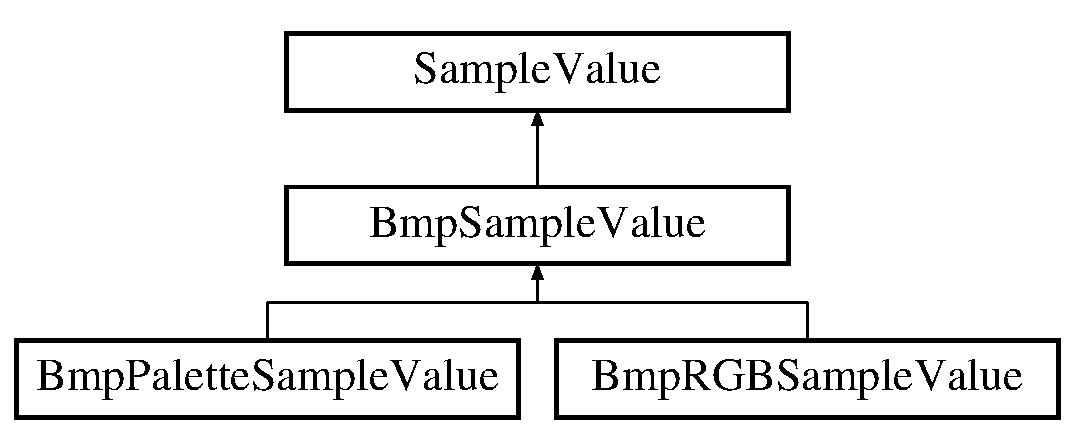
\includegraphics[height=3.000000cm]{classBmpSampleValue}
\end{center}
\end{figure}
\subsection*{Public Member Functions}
\begin{DoxyCompactItemize}
\item 
\textbf{ Bmp\+Sample\+Value} (void)
\item 
virtual \textbf{ U\+W\+O\+R\+D32} \textbf{ calc\+Distance} (const \textbf{ Sample\+Value} $\ast$s) const
\item 
virtual unsigned char \textbf{ get\+Red} (void) const =0
\item 
virtual unsigned char \textbf{ get\+Green} (void) const =0
\item 
virtual unsigned char \textbf{ get\+Blue} (void) const =0
\end{DoxyCompactItemize}
\subsection*{Additional Inherited Members}


\subsection{Constructor \& Destructor Documentation}
\mbox{\label{classBmpSampleValue_a088339541abf3b4511e71778633b6b12}} 
\index{Bmp\+Sample\+Value@{Bmp\+Sample\+Value}!Bmp\+Sample\+Value@{Bmp\+Sample\+Value}}
\index{Bmp\+Sample\+Value@{Bmp\+Sample\+Value}!Bmp\+Sample\+Value@{Bmp\+Sample\+Value}}
\subsubsection{Bmp\+Sample\+Value()}
{\footnotesize\ttfamily Bmp\+Sample\+Value\+::\+Bmp\+Sample\+Value (\begin{DoxyParamCaption}\item[{void}]{ }\end{DoxyParamCaption})\hspace{0.3cm}{\ttfamily [inline]}}



\subsection{Member Function Documentation}
\mbox{\label{classBmpSampleValue_af81c03b48ec98543a9e1a88b69b83abd}} 
\index{Bmp\+Sample\+Value@{Bmp\+Sample\+Value}!calc\+Distance@{calc\+Distance}}
\index{calc\+Distance@{calc\+Distance}!Bmp\+Sample\+Value@{Bmp\+Sample\+Value}}
\subsubsection{calc\+Distance()}
{\footnotesize\ttfamily \textbf{ U\+W\+O\+R\+D32} Bmp\+Sample\+Value\+::calc\+Distance (\begin{DoxyParamCaption}\item[{const \textbf{ Sample\+Value} $\ast$}]{s }\end{DoxyParamCaption}) const\hspace{0.3cm}{\ttfamily [virtual]}}

calculate the distance between the sample value s and this sample value 
\begin{DoxyParams}{Parameters}
{\em s} & a sample value of the same type as this \\
\hline
\end{DoxyParams}
\begin{DoxyReturn}{Returns}
the distance 
\end{DoxyReturn}


Implements \textbf{ Sample\+Value} \doxyref{}{p.}{classSampleValue_aa7e5d9b69203f6f6edf97c79319232dd}.



Reimplemented in \textbf{ Bmp\+R\+G\+B\+Sample\+Value} \doxyref{}{p.}{classBmpRGBSampleValue_a41c765b2108e640d3e7249f5dfd81eef}.

\mbox{\label{classBmpSampleValue_a0c31d4428158c7c6017935ac03254b26}} 
\index{Bmp\+Sample\+Value@{Bmp\+Sample\+Value}!get\+Blue@{get\+Blue}}
\index{get\+Blue@{get\+Blue}!Bmp\+Sample\+Value@{Bmp\+Sample\+Value}}
\subsubsection{get\+Blue()}
{\footnotesize\ttfamily virtual unsigned char Bmp\+Sample\+Value\+::get\+Blue (\begin{DoxyParamCaption}\item[{void}]{ }\end{DoxyParamCaption}) const\hspace{0.3cm}{\ttfamily [pure virtual]}}

get the blue color component 

Implemented in \textbf{ Bmp\+Palette\+Sample\+Value} \doxyref{}{p.}{classBmpPaletteSampleValue_aba2549aa10e39b580488e0c4625720c0}, and \textbf{ Bmp\+R\+G\+B\+Sample\+Value} \doxyref{}{p.}{classBmpRGBSampleValue_a35de04de107bf2a1f66f53eac3ab2b8d}.

\mbox{\label{classBmpSampleValue_a5d646a4082648a5b63323167553066ab}} 
\index{Bmp\+Sample\+Value@{Bmp\+Sample\+Value}!get\+Green@{get\+Green}}
\index{get\+Green@{get\+Green}!Bmp\+Sample\+Value@{Bmp\+Sample\+Value}}
\subsubsection{get\+Green()}
{\footnotesize\ttfamily virtual unsigned char Bmp\+Sample\+Value\+::get\+Green (\begin{DoxyParamCaption}\item[{void}]{ }\end{DoxyParamCaption}) const\hspace{0.3cm}{\ttfamily [pure virtual]}}

get the green color component 

Implemented in \textbf{ Bmp\+Palette\+Sample\+Value} \doxyref{}{p.}{classBmpPaletteSampleValue_a886c54100ed64d4bfd732b4be4ddae67}, and \textbf{ Bmp\+R\+G\+B\+Sample\+Value} \doxyref{}{p.}{classBmpRGBSampleValue_a9c1418294f6552b218a05a2439ee5df0}.

\mbox{\label{classBmpSampleValue_a8665a4c4db9ac910abf4ec0738cfde68}} 
\index{Bmp\+Sample\+Value@{Bmp\+Sample\+Value}!get\+Red@{get\+Red}}
\index{get\+Red@{get\+Red}!Bmp\+Sample\+Value@{Bmp\+Sample\+Value}}
\subsubsection{get\+Red()}
{\footnotesize\ttfamily virtual unsigned char Bmp\+Sample\+Value\+::get\+Red (\begin{DoxyParamCaption}\item[{void}]{ }\end{DoxyParamCaption}) const\hspace{0.3cm}{\ttfamily [pure virtual]}}

get the red color component 

Implemented in \textbf{ Bmp\+Palette\+Sample\+Value} \doxyref{}{p.}{classBmpPaletteSampleValue_a168e95b6da4f8aa4216fde934d561660}, and \textbf{ Bmp\+R\+G\+B\+Sample\+Value} \doxyref{}{p.}{classBmpRGBSampleValue_a8cbb5d220b2be0d1b9239d7abcda3a55}.



The documentation for this class was generated from the following files\+:\begin{DoxyCompactItemize}
\item 
\textbf{ Bmp\+Sample\+Value.\+h}\item 
\textbf{ Bmp\+Sample\+Value.\+cc}\end{DoxyCompactItemize}

\section{Bmp\+Win\+File\+Test Class Reference}
\label{classBmpWinFileTest}\index{Bmp\+Win\+File\+Test@{Bmp\+Win\+File\+Test}}


{\ttfamily \#include $<$Bmp\+Win\+File\+Test.\+h$>$}

Inheritance diagram for Bmp\+Win\+File\+Test\+:\begin{figure}[H]
\begin{center}
\leavevmode
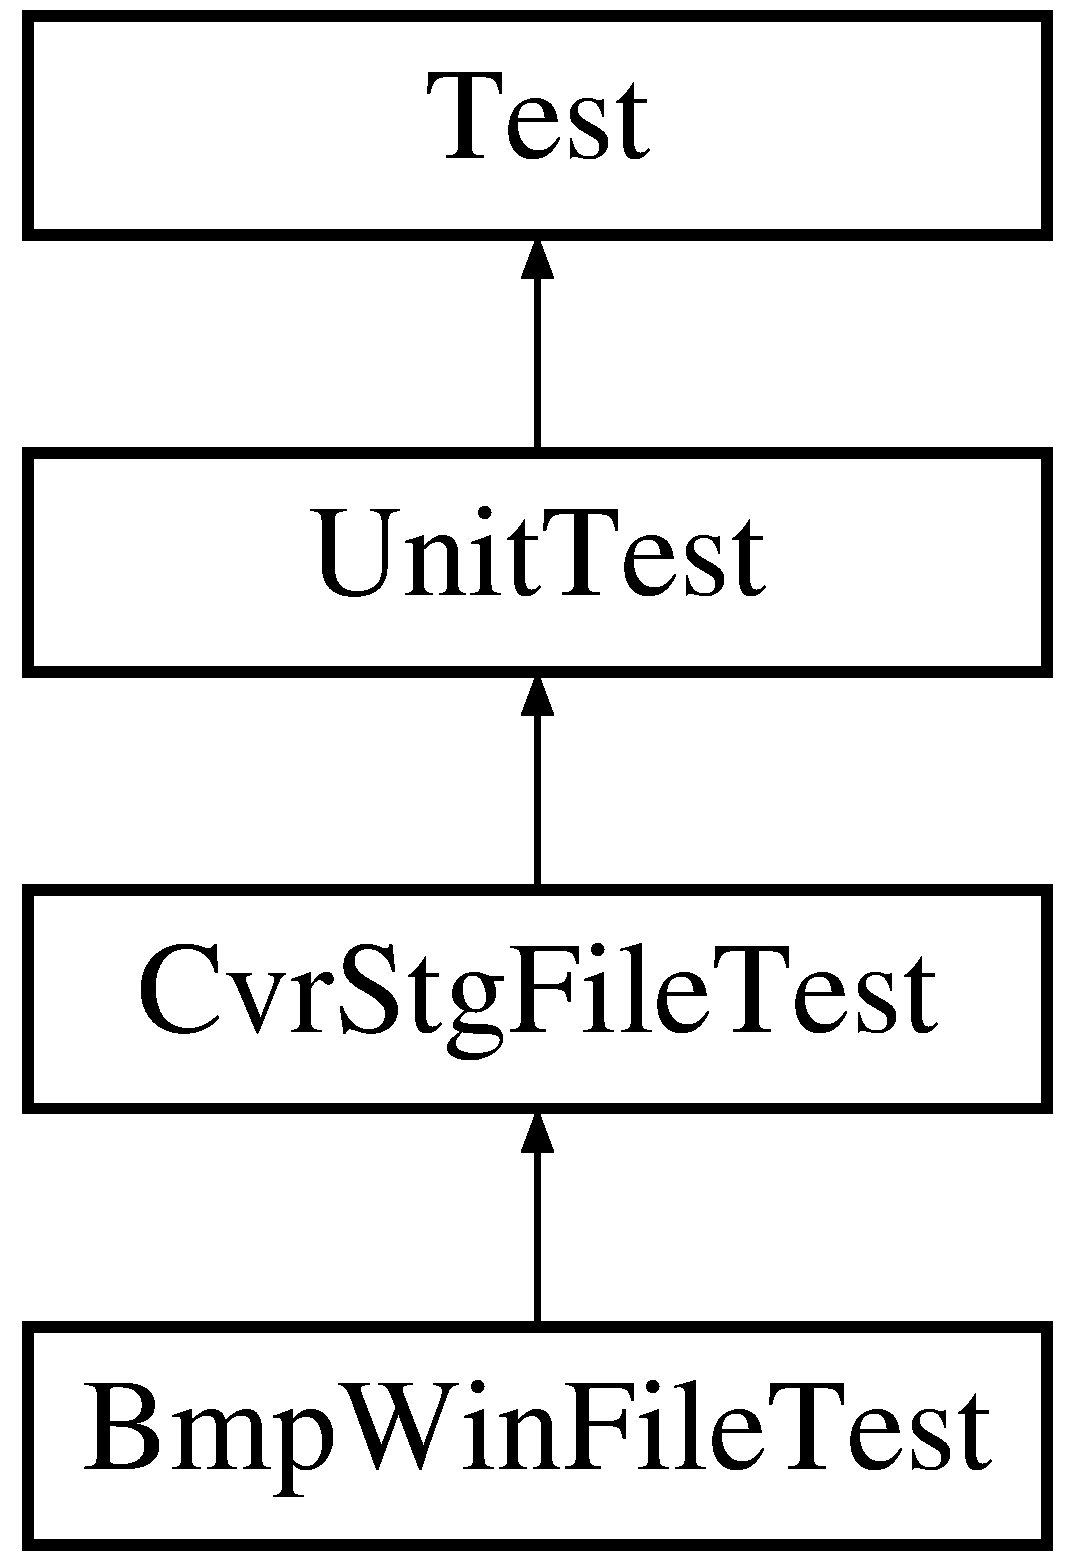
\includegraphics[height=4.000000cm]{classBmpWinFileTest}
\end{center}
\end{figure}
\subsection*{Public Member Functions}
\begin{DoxyCompactItemize}
\item 
\textbf{ Bmp\+Win\+File\+Test} (\textbf{ Test\+Suite} $\ast$s)
\item 
void \textbf{ setup} (void)
\item 
void \textbf{ cleanup} (void)
\item 
void \textbf{ test\+Read\+Write} (void)
\item 
void \textbf{ test\+Read\+Embed\+Extract} (void)
\item 
void \textbf{ test\+Read\+Embed\+Write\+Read\+Extract} (void)
\item 
void \textbf{ test\+Position} (void)
\item 
void \textbf{ test\+Read\+Extract\+Compare} (void)
\item 
void \textbf{ test\+Embedded\+Value} (void)
\end{DoxyCompactItemize}
\subsection*{Private Attributes}
\begin{DoxyCompactItemize}
\item 
\textbf{ Bit\+String} $\ast$ \textbf{ bs1}
\item 
\textbf{ Bit\+String} $\ast$ \textbf{ bs2}
\item 
\textbf{ Bit\+String} $\ast$ \textbf{ bs3}
\item 
\textbf{ Bit\+String} $\ast$ \textbf{ bs4}
\item 
\textbf{ Cvr\+Stg\+File} $\ast$ \textbf{ f1}
\item 
\textbf{ Cvr\+Stg\+File} $\ast$ \textbf{ f2}
\item 
\textbf{ Cvr\+Stg\+File} $\ast$ \textbf{ f3}
\item 
\textbf{ Cvr\+Stg\+File} $\ast$ \textbf{ f4}
\item 
\textbf{ Globals} \textbf{ gl1}
\item 
\textbf{ Globals} \textbf{ gl2}
\item 
\textbf{ Globals} \textbf{ gl3}
\item 
\textbf{ Globals} \textbf{ gl4}
\end{DoxyCompactItemize}
\subsection*{Additional Inherited Members}


\subsection{Constructor \& Destructor Documentation}
\mbox{\label{classBmpWinFileTest_a945970f163b5f4f980e1a22fa80c0db0}} 
\index{Bmp\+Win\+File\+Test@{Bmp\+Win\+File\+Test}!Bmp\+Win\+File\+Test@{Bmp\+Win\+File\+Test}}
\index{Bmp\+Win\+File\+Test@{Bmp\+Win\+File\+Test}!Bmp\+Win\+File\+Test@{Bmp\+Win\+File\+Test}}
\subsubsection{Bmp\+Win\+File\+Test()}
{\footnotesize\ttfamily Bmp\+Win\+File\+Test\+::\+Bmp\+Win\+File\+Test (\begin{DoxyParamCaption}\item[{\textbf{ Test\+Suite} $\ast$}]{s }\end{DoxyParamCaption})}



\subsection{Member Function Documentation}
\mbox{\label{classBmpWinFileTest_a75851865ed9731498fef7a646ad516f1}} 
\index{Bmp\+Win\+File\+Test@{Bmp\+Win\+File\+Test}!cleanup@{cleanup}}
\index{cleanup@{cleanup}!Bmp\+Win\+File\+Test@{Bmp\+Win\+File\+Test}}
\subsubsection{cleanup()}
{\footnotesize\ttfamily void Bmp\+Win\+File\+Test\+::cleanup (\begin{DoxyParamCaption}\item[{void}]{ }\end{DoxyParamCaption})\hspace{0.3cm}{\ttfamily [virtual]}}

cleanup the unit test -\/ called after run 

Reimplemented from \textbf{ Unit\+Test} \doxyref{}{p.}{classUnitTest_adf77efe972ee4a766d94e3f7ddc193ad}.

\mbox{\label{classBmpWinFileTest_a2e131bfb54e7e4e7e653d5dc55488e4e}} 
\index{Bmp\+Win\+File\+Test@{Bmp\+Win\+File\+Test}!setup@{setup}}
\index{setup@{setup}!Bmp\+Win\+File\+Test@{Bmp\+Win\+File\+Test}}
\subsubsection{setup()}
{\footnotesize\ttfamily void Bmp\+Win\+File\+Test\+::setup (\begin{DoxyParamCaption}\item[{void}]{ }\end{DoxyParamCaption})\hspace{0.3cm}{\ttfamily [virtual]}}

setup the unit test -\/ called before run

\doxyref{Unit\+Test\+::setup}{p.}{classUnitTest_ad73fdf9012b651047ea001d21f9d27ad} will (together with \doxyref{Unit\+Test\+::cleanup}{p.}{classUnitTest_adf77efe972ee4a766d94e3f7ddc193ad}) save and restore the object stored in Globs so they should be called from the corresponding functions in the derived object if the derived unit test manipulates the Globs object. 

Reimplemented from \textbf{ Unit\+Test} \doxyref{}{p.}{classUnitTest_ad73fdf9012b651047ea001d21f9d27ad}.

\mbox{\label{classBmpWinFileTest_a572e649e25fead7151db3f610d3cd6b6}} 
\index{Bmp\+Win\+File\+Test@{Bmp\+Win\+File\+Test}!test\+Embedded\+Value@{test\+Embedded\+Value}}
\index{test\+Embedded\+Value@{test\+Embedded\+Value}!Bmp\+Win\+File\+Test@{Bmp\+Win\+File\+Test}}
\subsubsection{test\+Embedded\+Value()}
{\footnotesize\ttfamily void Bmp\+Win\+File\+Test\+::test\+Embedded\+Value (\begin{DoxyParamCaption}\item[{void}]{ }\end{DoxyParamCaption})}

\mbox{\label{classBmpWinFileTest_a2b243ee511ae76c80a39090e1046e659}} 
\index{Bmp\+Win\+File\+Test@{Bmp\+Win\+File\+Test}!test\+Position@{test\+Position}}
\index{test\+Position@{test\+Position}!Bmp\+Win\+File\+Test@{Bmp\+Win\+File\+Test}}
\subsubsection{test\+Position()}
{\footnotesize\ttfamily void Bmp\+Win\+File\+Test\+::test\+Position (\begin{DoxyParamCaption}\item[{void}]{ }\end{DoxyParamCaption})}

\mbox{\label{classBmpWinFileTest_a9be730ad4db7a1c01bbd4eadf6648787}} 
\index{Bmp\+Win\+File\+Test@{Bmp\+Win\+File\+Test}!test\+Read\+Embed\+Extract@{test\+Read\+Embed\+Extract}}
\index{test\+Read\+Embed\+Extract@{test\+Read\+Embed\+Extract}!Bmp\+Win\+File\+Test@{Bmp\+Win\+File\+Test}}
\subsubsection{test\+Read\+Embed\+Extract()}
{\footnotesize\ttfamily void Bmp\+Win\+File\+Test\+::test\+Read\+Embed\+Extract (\begin{DoxyParamCaption}\item[{void}]{ }\end{DoxyParamCaption})}

\mbox{\label{classBmpWinFileTest_a9380ae183e1a42b3699fa81f4f6fa3b8}} 
\index{Bmp\+Win\+File\+Test@{Bmp\+Win\+File\+Test}!test\+Read\+Embed\+Write\+Read\+Extract@{test\+Read\+Embed\+Write\+Read\+Extract}}
\index{test\+Read\+Embed\+Write\+Read\+Extract@{test\+Read\+Embed\+Write\+Read\+Extract}!Bmp\+Win\+File\+Test@{Bmp\+Win\+File\+Test}}
\subsubsection{test\+Read\+Embed\+Write\+Read\+Extract()}
{\footnotesize\ttfamily void Bmp\+Win\+File\+Test\+::test\+Read\+Embed\+Write\+Read\+Extract (\begin{DoxyParamCaption}\item[{void}]{ }\end{DoxyParamCaption})}

\mbox{\label{classBmpWinFileTest_adc27e7f9c4b6b23fcedfb3e0f95e2088}} 
\index{Bmp\+Win\+File\+Test@{Bmp\+Win\+File\+Test}!test\+Read\+Extract\+Compare@{test\+Read\+Extract\+Compare}}
\index{test\+Read\+Extract\+Compare@{test\+Read\+Extract\+Compare}!Bmp\+Win\+File\+Test@{Bmp\+Win\+File\+Test}}
\subsubsection{test\+Read\+Extract\+Compare()}
{\footnotesize\ttfamily void Bmp\+Win\+File\+Test\+::test\+Read\+Extract\+Compare (\begin{DoxyParamCaption}\item[{void}]{ }\end{DoxyParamCaption})}

\mbox{\label{classBmpWinFileTest_a4c5976725ff8b32b536620d083128236}} 
\index{Bmp\+Win\+File\+Test@{Bmp\+Win\+File\+Test}!test\+Read\+Write@{test\+Read\+Write}}
\index{test\+Read\+Write@{test\+Read\+Write}!Bmp\+Win\+File\+Test@{Bmp\+Win\+File\+Test}}
\subsubsection{test\+Read\+Write()}
{\footnotesize\ttfamily void Bmp\+Win\+File\+Test\+::test\+Read\+Write (\begin{DoxyParamCaption}\item[{void}]{ }\end{DoxyParamCaption})}



\subsection{Member Data Documentation}
\mbox{\label{classBmpWinFileTest_a0e099b3ae80671fda863075c88991a28}} 
\index{Bmp\+Win\+File\+Test@{Bmp\+Win\+File\+Test}!bs1@{bs1}}
\index{bs1@{bs1}!Bmp\+Win\+File\+Test@{Bmp\+Win\+File\+Test}}
\subsubsection{bs1}
{\footnotesize\ttfamily \textbf{ Bit\+String}$\ast$ Bmp\+Win\+File\+Test\+::bs1\hspace{0.3cm}{\ttfamily [private]}}

\mbox{\label{classBmpWinFileTest_ad1c9b22e926b8ec4baeb5eda81a0d5ca}} 
\index{Bmp\+Win\+File\+Test@{Bmp\+Win\+File\+Test}!bs2@{bs2}}
\index{bs2@{bs2}!Bmp\+Win\+File\+Test@{Bmp\+Win\+File\+Test}}
\subsubsection{bs2}
{\footnotesize\ttfamily \textbf{ Bit\+String} $\ast$ Bmp\+Win\+File\+Test\+::bs2\hspace{0.3cm}{\ttfamily [private]}}

\mbox{\label{classBmpWinFileTest_a5c40929a79edddd31e44e9b57da8e6e8}} 
\index{Bmp\+Win\+File\+Test@{Bmp\+Win\+File\+Test}!bs3@{bs3}}
\index{bs3@{bs3}!Bmp\+Win\+File\+Test@{Bmp\+Win\+File\+Test}}
\subsubsection{bs3}
{\footnotesize\ttfamily \textbf{ Bit\+String} $\ast$ Bmp\+Win\+File\+Test\+::bs3\hspace{0.3cm}{\ttfamily [private]}}

\mbox{\label{classBmpWinFileTest_a358ad1376305bb17ecb6214d94034114}} 
\index{Bmp\+Win\+File\+Test@{Bmp\+Win\+File\+Test}!bs4@{bs4}}
\index{bs4@{bs4}!Bmp\+Win\+File\+Test@{Bmp\+Win\+File\+Test}}
\subsubsection{bs4}
{\footnotesize\ttfamily \textbf{ Bit\+String} $\ast$ Bmp\+Win\+File\+Test\+::bs4\hspace{0.3cm}{\ttfamily [private]}}

\mbox{\label{classBmpWinFileTest_afd10c363d5f78e762fa69867b23e33ce}} 
\index{Bmp\+Win\+File\+Test@{Bmp\+Win\+File\+Test}!f1@{f1}}
\index{f1@{f1}!Bmp\+Win\+File\+Test@{Bmp\+Win\+File\+Test}}
\subsubsection{f1}
{\footnotesize\ttfamily \textbf{ Cvr\+Stg\+File}$\ast$ Bmp\+Win\+File\+Test\+::f1\hspace{0.3cm}{\ttfamily [private]}}

\mbox{\label{classBmpWinFileTest_a3c4cdb8ddd8454c76a7e9343c260c3fd}} 
\index{Bmp\+Win\+File\+Test@{Bmp\+Win\+File\+Test}!f2@{f2}}
\index{f2@{f2}!Bmp\+Win\+File\+Test@{Bmp\+Win\+File\+Test}}
\subsubsection{f2}
{\footnotesize\ttfamily \textbf{ Cvr\+Stg\+File} $\ast$ Bmp\+Win\+File\+Test\+::f2\hspace{0.3cm}{\ttfamily [private]}}

\mbox{\label{classBmpWinFileTest_ad31596b2761c0bbc07347e3c0b5e35b8}} 
\index{Bmp\+Win\+File\+Test@{Bmp\+Win\+File\+Test}!f3@{f3}}
\index{f3@{f3}!Bmp\+Win\+File\+Test@{Bmp\+Win\+File\+Test}}
\subsubsection{f3}
{\footnotesize\ttfamily \textbf{ Cvr\+Stg\+File} $\ast$ Bmp\+Win\+File\+Test\+::f3\hspace{0.3cm}{\ttfamily [private]}}

\mbox{\label{classBmpWinFileTest_afb4a7b7a0608acb8a6dd9dfe338f1ad8}} 
\index{Bmp\+Win\+File\+Test@{Bmp\+Win\+File\+Test}!f4@{f4}}
\index{f4@{f4}!Bmp\+Win\+File\+Test@{Bmp\+Win\+File\+Test}}
\subsubsection{f4}
{\footnotesize\ttfamily \textbf{ Cvr\+Stg\+File} $\ast$ Bmp\+Win\+File\+Test\+::f4\hspace{0.3cm}{\ttfamily [private]}}

\mbox{\label{classBmpWinFileTest_ae22e7611e260bb37f738c69f5c5d8ba8}} 
\index{Bmp\+Win\+File\+Test@{Bmp\+Win\+File\+Test}!gl1@{gl1}}
\index{gl1@{gl1}!Bmp\+Win\+File\+Test@{Bmp\+Win\+File\+Test}}
\subsubsection{gl1}
{\footnotesize\ttfamily \textbf{ Globals} Bmp\+Win\+File\+Test\+::gl1\hspace{0.3cm}{\ttfamily [private]}}

\mbox{\label{classBmpWinFileTest_a3b7d3dc5aa609a827e056edbe5c1ed6f}} 
\index{Bmp\+Win\+File\+Test@{Bmp\+Win\+File\+Test}!gl2@{gl2}}
\index{gl2@{gl2}!Bmp\+Win\+File\+Test@{Bmp\+Win\+File\+Test}}
\subsubsection{gl2}
{\footnotesize\ttfamily \textbf{ Globals} Bmp\+Win\+File\+Test\+::gl2\hspace{0.3cm}{\ttfamily [private]}}

\mbox{\label{classBmpWinFileTest_a7f952778c52eccc057f824fb32462a93}} 
\index{Bmp\+Win\+File\+Test@{Bmp\+Win\+File\+Test}!gl3@{gl3}}
\index{gl3@{gl3}!Bmp\+Win\+File\+Test@{Bmp\+Win\+File\+Test}}
\subsubsection{gl3}
{\footnotesize\ttfamily \textbf{ Globals} Bmp\+Win\+File\+Test\+::gl3\hspace{0.3cm}{\ttfamily [private]}}

\mbox{\label{classBmpWinFileTest_acfb018af0f85c976203053196d291572}} 
\index{Bmp\+Win\+File\+Test@{Bmp\+Win\+File\+Test}!gl4@{gl4}}
\index{gl4@{gl4}!Bmp\+Win\+File\+Test@{Bmp\+Win\+File\+Test}}
\subsubsection{gl4}
{\footnotesize\ttfamily \textbf{ Globals} Bmp\+Win\+File\+Test\+::gl4\hspace{0.3cm}{\ttfamily [private]}}



The documentation for this class was generated from the following files\+:\begin{DoxyCompactItemize}
\item 
\textbf{ Bmp\+Win\+File\+Test.\+h}\item 
\textbf{ Bmp\+Win\+File\+Test.\+cc}\end{DoxyCompactItemize}

\section{Color\+Palette Class Reference}
\label{classColorPalette}\index{Color\+Palette@{Color\+Palette}}


a color palette  




{\ttfamily \#include $<$Color\+Palette.\+h$>$}

Inheritance diagram for Color\+Palette\+:\begin{figure}[H]
\begin{center}
\leavevmode
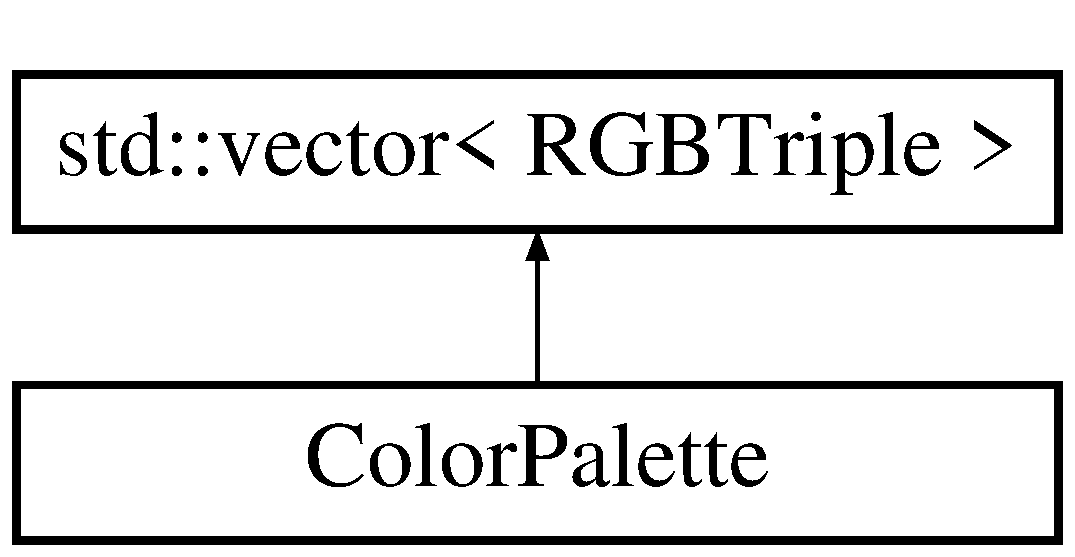
\includegraphics[height=2.000000cm]{classColorPalette}
\end{center}
\end{figure}
\subsection*{Public Member Functions}
\begin{DoxyCompactItemize}
\item 
unsigned int \textbf{ get\+Size} (void) const
\item 
void \textbf{ add\+Entry} (\textbf{ R\+G\+B\+Triple} rgb)
\item 
void \textbf{ add\+Entry} (\textbf{ B\+Y\+TE} r, \textbf{ B\+Y\+TE} g, \textbf{ B\+Y\+TE} b)
\end{DoxyCompactItemize}


\subsection{Detailed Description}
This class is essentially a vector$<$\+R\+G\+B\+Triple$>$ with some wrappers for exisiting methods. 

\subsection{Member Function Documentation}
\mbox{\label{classColorPalette_a1aee942b853cb4dedc2f2b57bb82542b}} 
\index{Color\+Palette@{Color\+Palette}!add\+Entry@{add\+Entry}}
\index{add\+Entry@{add\+Entry}!Color\+Palette@{Color\+Palette}}
\subsubsection{add\+Entry()\hspace{0.1cm}{\footnotesize\ttfamily [1/2]}}
{\footnotesize\ttfamily void Color\+Palette\+::add\+Entry (\begin{DoxyParamCaption}\item[{\textbf{ R\+G\+B\+Triple}}]{rgb }\end{DoxyParamCaption})\hspace{0.3cm}{\ttfamily [inline]}}

add (a copy of) rgb to the end of this color palette \mbox{\label{classColorPalette_abc424ad9e51c0c35b252f17e339de0ff}} 
\index{Color\+Palette@{Color\+Palette}!add\+Entry@{add\+Entry}}
\index{add\+Entry@{add\+Entry}!Color\+Palette@{Color\+Palette}}
\subsubsection{add\+Entry()\hspace{0.1cm}{\footnotesize\ttfamily [2/2]}}
{\footnotesize\ttfamily void Color\+Palette\+::add\+Entry (\begin{DoxyParamCaption}\item[{\textbf{ B\+Y\+TE}}]{r,  }\item[{\textbf{ B\+Y\+TE}}]{g,  }\item[{\textbf{ B\+Y\+TE}}]{b }\end{DoxyParamCaption})\hspace{0.3cm}{\ttfamily [inline]}}

add the color r/g/b to the end of this color palette \mbox{\label{classColorPalette_aeaf501154a206ffb2080aaba22de6db8}} 
\index{Color\+Palette@{Color\+Palette}!get\+Size@{get\+Size}}
\index{get\+Size@{get\+Size}!Color\+Palette@{Color\+Palette}}
\subsubsection{get\+Size()}
{\footnotesize\ttfamily unsigned int Color\+Palette\+::get\+Size (\begin{DoxyParamCaption}\item[{void}]{ }\end{DoxyParamCaption}) const\hspace{0.3cm}{\ttfamily [inline]}}

get the size, i.\+e. the number of entries of this color palette 

The documentation for this class was generated from the following file\+:\begin{DoxyCompactItemize}
\item 
\textbf{ Color\+Palette.\+h}\end{DoxyCompactItemize}

\section{Corrupt\+Data\+Error Class Reference}
\label{classCorruptDataError}\index{Corrupt\+Data\+Error@{Corrupt\+Data\+Error}}


is thrown as exception when corrupt data is encountered during extraction  




{\ttfamily \#include $<$error.\+h$>$}

Inheritance diagram for Corrupt\+Data\+Error\+:\begin{figure}[H]
\begin{center}
\leavevmode
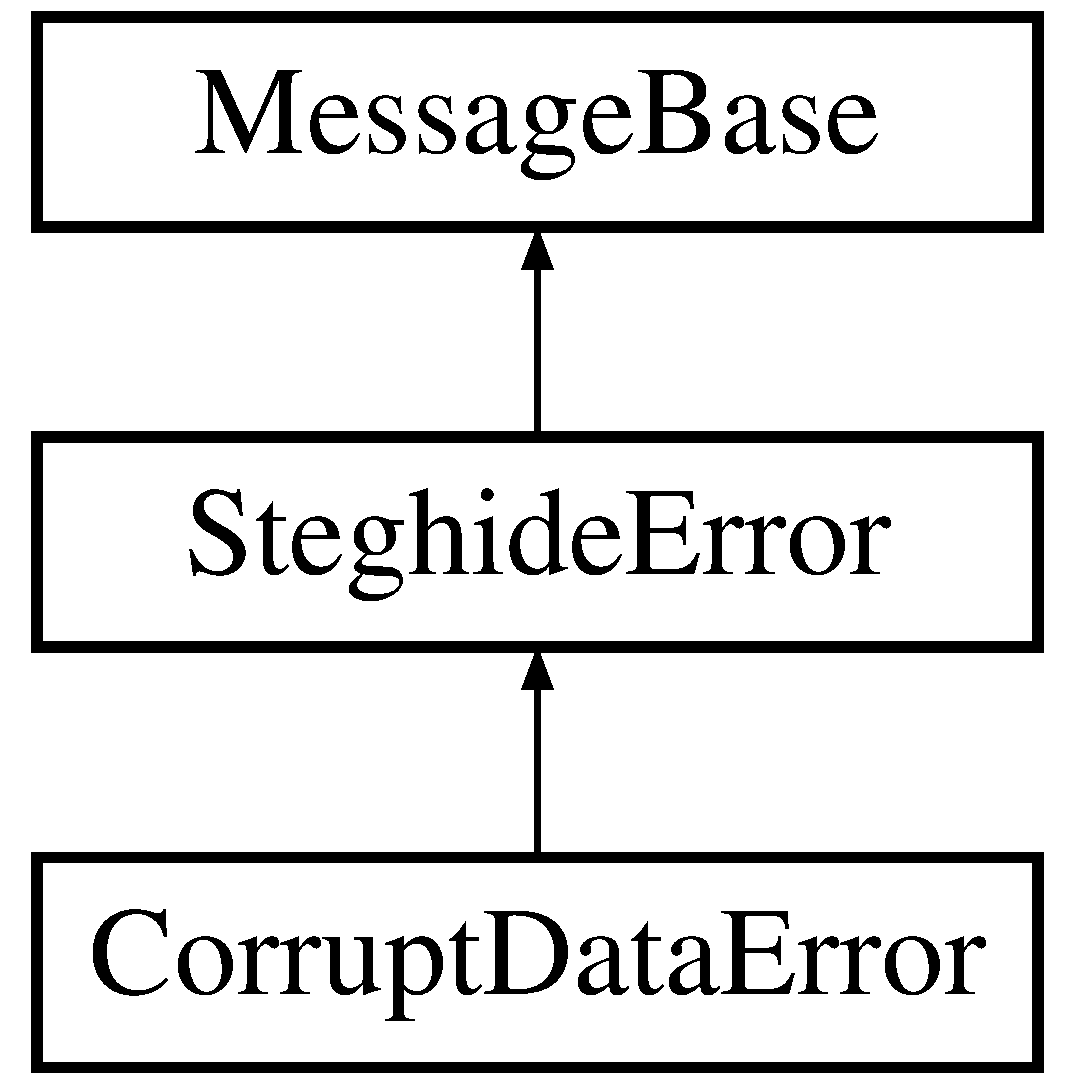
\includegraphics[height=3.000000cm]{classCorruptDataError}
\end{center}
\end{figure}
\subsection*{Public Member Functions}
\begin{DoxyCompactItemize}
\item 
\textbf{ Corrupt\+Data\+Error} (const char $\ast$msgfmt,...)
\item 
void \textbf{ print\+Message} (void) const
\end{DoxyCompactItemize}
\subsection*{Additional Inherited Members}


\subsection{Detailed Description}
A possible cause of this exception being thrown is a wrong password. 

\subsection{Constructor \& Destructor Documentation}
\mbox{\label{classCorruptDataError_a2301d275cf15c4b83d12e6632ad086f4}} 
\index{Corrupt\+Data\+Error@{Corrupt\+Data\+Error}!Corrupt\+Data\+Error@{Corrupt\+Data\+Error}}
\index{Corrupt\+Data\+Error@{Corrupt\+Data\+Error}!Corrupt\+Data\+Error@{Corrupt\+Data\+Error}}
\subsubsection{Corrupt\+Data\+Error()}
{\footnotesize\ttfamily Corrupt\+Data\+Error\+::\+Corrupt\+Data\+Error (\begin{DoxyParamCaption}\item[{const char $\ast$}]{msgfmt,  }\item[{}]{... }\end{DoxyParamCaption})}



\subsection{Member Function Documentation}
\mbox{\label{classCorruptDataError_a345998f46c50877c96d40c1d349f2a1a}} 
\index{Corrupt\+Data\+Error@{Corrupt\+Data\+Error}!print\+Message@{print\+Message}}
\index{print\+Message@{print\+Message}!Corrupt\+Data\+Error@{Corrupt\+Data\+Error}}
\subsubsection{print\+Message()}
{\footnotesize\ttfamily void Corrupt\+Data\+Error\+::print\+Message (\begin{DoxyParamCaption}\item[{void}]{ }\end{DoxyParamCaption}) const\hspace{0.3cm}{\ttfamily [virtual]}}



Reimplemented from \textbf{ Steghide\+Error} \doxyref{}{p.}{classSteghideError_a22d688da944706920f51159ebd0076d9}.



The documentation for this class was generated from the following files\+:\begin{DoxyCompactItemize}
\item 
\textbf{ error.\+h}\item 
\textbf{ error.\+cc}\end{DoxyCompactItemize}

\section{Critical\+Warning Class Reference}
\label{classCriticalWarning}\index{Critical\+Warning@{Critical\+Warning}}


{\ttfamily \#include $<$msg.\+h$>$}

Inheritance diagram for Critical\+Warning\+:\begin{figure}[H]
\begin{center}
\leavevmode
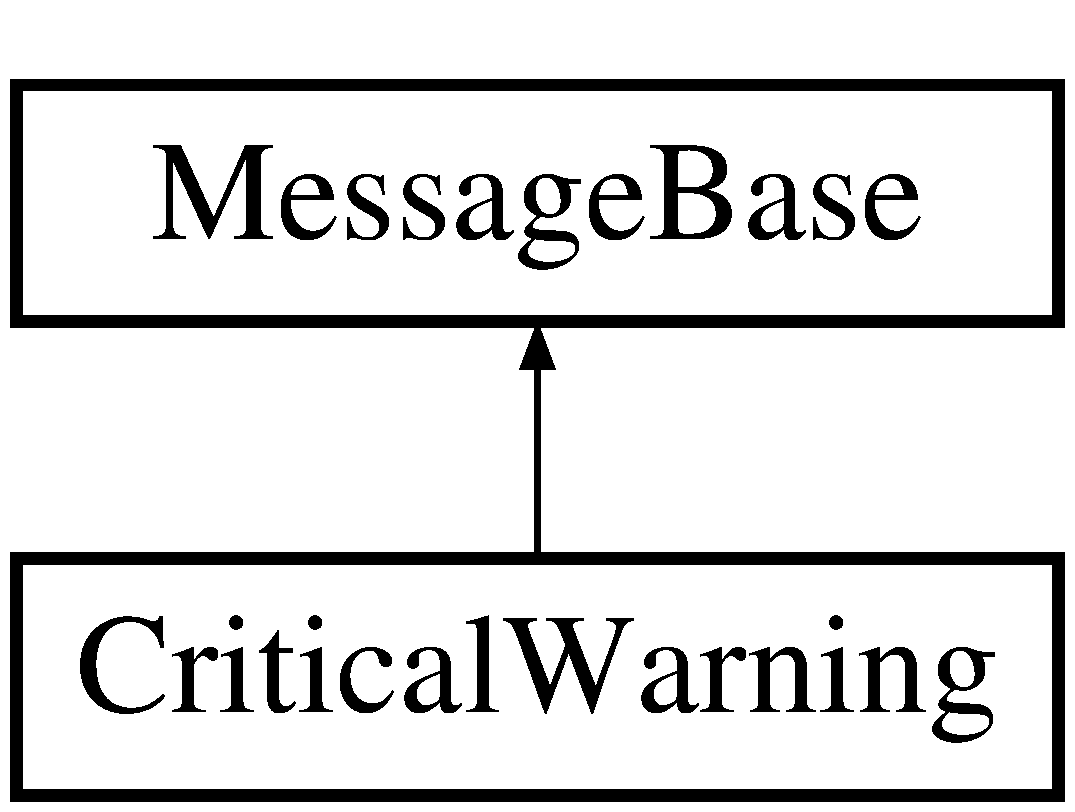
\includegraphics[height=2.000000cm]{classCriticalWarning}
\end{center}
\end{figure}
\subsection*{Public Member Functions}
\begin{DoxyCompactItemize}
\item 
\textbf{ Critical\+Warning} (void)
\item 
\textbf{ Critical\+Warning} (std\+::string msg)
\item 
\textbf{ Critical\+Warning} (const char $\ast$msgfmt,...)
\item 
void \textbf{ print\+Message} (void) const
\end{DoxyCompactItemize}
\subsection*{Additional Inherited Members}


\subsection{Constructor \& Destructor Documentation}
\mbox{\label{classCriticalWarning_a7f66897443acfa4c041f63d2ee7a7b4b}} 
\index{Critical\+Warning@{Critical\+Warning}!Critical\+Warning@{Critical\+Warning}}
\index{Critical\+Warning@{Critical\+Warning}!Critical\+Warning@{Critical\+Warning}}
\subsubsection{Critical\+Warning()\hspace{0.1cm}{\footnotesize\ttfamily [1/3]}}
{\footnotesize\ttfamily Critical\+Warning\+::\+Critical\+Warning (\begin{DoxyParamCaption}\item[{void}]{ }\end{DoxyParamCaption})\hspace{0.3cm}{\ttfamily [inline]}}

\mbox{\label{classCriticalWarning_a5f06fd14700d4d68655f72ee61a926b4}} 
\index{Critical\+Warning@{Critical\+Warning}!Critical\+Warning@{Critical\+Warning}}
\index{Critical\+Warning@{Critical\+Warning}!Critical\+Warning@{Critical\+Warning}}
\subsubsection{Critical\+Warning()\hspace{0.1cm}{\footnotesize\ttfamily [2/3]}}
{\footnotesize\ttfamily Critical\+Warning\+::\+Critical\+Warning (\begin{DoxyParamCaption}\item[{std\+::string}]{msg }\end{DoxyParamCaption})\hspace{0.3cm}{\ttfamily [inline]}}

\mbox{\label{classCriticalWarning_ac4c8c1da27e7a99ac5eb13fada159531}} 
\index{Critical\+Warning@{Critical\+Warning}!Critical\+Warning@{Critical\+Warning}}
\index{Critical\+Warning@{Critical\+Warning}!Critical\+Warning@{Critical\+Warning}}
\subsubsection{Critical\+Warning()\hspace{0.1cm}{\footnotesize\ttfamily [3/3]}}
{\footnotesize\ttfamily Critical\+Warning\+::\+Critical\+Warning (\begin{DoxyParamCaption}\item[{const char $\ast$}]{msgfmt,  }\item[{}]{... }\end{DoxyParamCaption})}



\subsection{Member Function Documentation}
\mbox{\label{classCriticalWarning_af92d1c346a1a0ec2a150a46d90afe2f5}} 
\index{Critical\+Warning@{Critical\+Warning}!print\+Message@{print\+Message}}
\index{print\+Message@{print\+Message}!Critical\+Warning@{Critical\+Warning}}
\subsubsection{print\+Message()}
{\footnotesize\ttfamily void Critical\+Warning\+::print\+Message (\begin{DoxyParamCaption}\item[{void}]{ }\end{DoxyParamCaption}) const\hspace{0.3cm}{\ttfamily [virtual]}}



Implements \textbf{ Message\+Base} \doxyref{}{p.}{classMessageBase_a207178190da2bec546a972495cdf9bc6}.



The documentation for this class was generated from the following files\+:\begin{DoxyCompactItemize}
\item 
\textbf{ msg.\+h}\item 
\textbf{ msg.\+cc}\end{DoxyCompactItemize}

\section{Cvr\+Stg\+File Class Reference}
\label{classCvrStgFile}\index{Cvr\+Stg\+File@{Cvr\+Stg\+File}}


a cover-\//stego-\/file  




{\ttfamily \#include $<$Cvr\+Stg\+File.\+h$>$}

Inheritance diagram for Cvr\+Stg\+File\+:\begin{figure}[H]
\begin{center}
\leavevmode
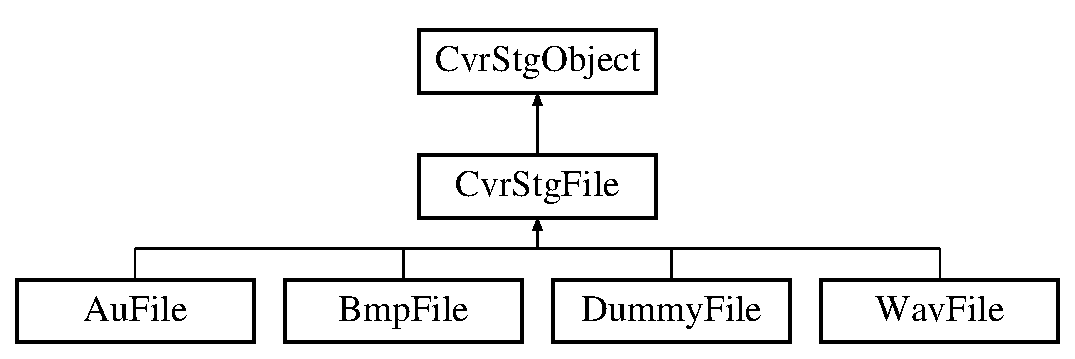
\includegraphics[height=3.000000cm]{classCvrStgFile}
\end{center}
\end{figure}
\subsection*{Classes}
\begin{DoxyCompactItemize}
\item 
class \textbf{ Property}
\end{DoxyCompactItemize}
\subsection*{Public Member Functions}
\begin{DoxyCompactItemize}
\item 
\textbf{ Cvr\+Stg\+File} (void)
\item 
virtual \textbf{ $\sim$\+Cvr\+Stg\+File} (void)
\item 
virtual void \textbf{ read} (\textbf{ Binary\+IO} $\ast$io)
\item 
virtual void \textbf{ write} (void)
\item 
void \textbf{ transform} (const std\+::string \&fn)
\item 
virtual std\+::list$<$ \textbf{ Property} $>$ \textbf{ get\+Properties} (void) const =0
\item 
virtual std\+::vector$<$ \textbf{ Sample\+Value\+Adjacency\+List} $\ast$ $>$ \textbf{ calc\+S\+V\+Adjacency\+Lists} (const std\+::vector$<$ \textbf{ Sample\+Value} $\ast$$>$ \&svs) const
\item 
virtual std\+::vector$<$ \textbf{ Matching\+Algorithm} $\ast$ $>$ \textbf{ get\+Matching\+Algorithms} (\textbf{ Graph} $\ast$g, \textbf{ Matching} $\ast$m) const
\item 
const std\+::string \& \textbf{ get\+Name} (void) const
\item 
bool \textbf{ is\+\_\+std} (void) const
\item 
unsigned long \textbf{ get\+Capacity} (void) const
\item 
std\+::string \textbf{ get\+H\+R\+Capacity} (void) const
\item 
unsigned short \textbf{ get\+Samples\+Per\+Vertex} (void) const
\item 
\textbf{ U\+W\+O\+R\+D32} \textbf{ get\+Radius} (void) const
\item 
\textbf{ Emb\+Value} \textbf{ get\+Emb\+Value\+Modulus} (void) const
\item 
virtual \textbf{ Emb\+Value} \textbf{ get\+Embedded\+Value} (const \textbf{ Sample\+Pos} pos) const
\end{DoxyCompactItemize}
\subsection*{Static Public Member Functions}
\begin{DoxyCompactItemize}
\item 
static \textbf{ Cvr\+Stg\+File} $\ast$ \textbf{ read\+File} (const std\+::string \&fn)
\end{DoxyCompactItemize}
\subsection*{Protected Member Functions}
\begin{DoxyCompactItemize}
\item 
void \textbf{ set\+Samples\+Per\+Vertex} (unsigned short spv)
\item 
void \textbf{ set\+Radius} (\textbf{ U\+W\+O\+R\+D32} r)
\item 
void \textbf{ set\+Emb\+Value\+Modulus} (\textbf{ Emb\+Value} m)
\item 
void \textbf{ set\+Bin\+IO} (\textbf{ Binary\+IO} $\ast$io)
\item 
\textbf{ Binary\+IO} $\ast$ \textbf{ get\+Bin\+IO} (void) const
\end{DoxyCompactItemize}
\subsection*{Private Types}
\begin{DoxyCompactItemize}
\item 
enum \textbf{ F\+I\+L\+E\+F\+O\+R\+M\+AT} \{ \newline
\textbf{ U\+N\+K\+N\+O\+WN}, 
\textbf{ B\+MP}, 
\textbf{ W\+AV}, 
\textbf{ AU}, 
\newline
\textbf{ J\+P\+EG}
 \}
\end{DoxyCompactItemize}
\subsection*{Static Private Member Functions}
\begin{DoxyCompactItemize}
\item 
static \textbf{ F\+I\+L\+E\+F\+O\+R\+M\+AT} \textbf{ guessff} (\textbf{ Binary\+IO} $\ast$io)
\end{DoxyCompactItemize}
\subsection*{Private Attributes}
\begin{DoxyCompactItemize}
\item 
\textbf{ Binary\+IO} $\ast$ \textbf{ Bin\+IO}
\item 
unsigned short \textbf{ Samples\+Per\+Vertex}
\item 
\textbf{ U\+W\+O\+R\+D32} \textbf{ Radius}
\item 
\textbf{ Emb\+Value} \textbf{ Emb\+Value\+Modulus}
\end{DoxyCompactItemize}


\subsection{Detailed Description}
file-\/format specific constants are handled as follows\+: \doxyref{Cvr\+Stg\+File}{p.}{classCvrStgFile} contains a protected set-\/function (e.\+g. set\+Samples\+Per\+Vertex), a public get-\/function (e.\+g. \doxyref{get\+Samples\+Per\+Vertex() const}{p.}{classCvrStgFile_a6bbcd17a373ddd6f45ced2909b658298}) and a private variable. The public get function does nothing else than returning the private variable, which must be set as soon as possible (if it is not set, it will contain a null value set in \doxyref{Cvr\+Stg\+File\+::\+Cvr\+Stg\+File}{p.}{classCvrStgFile_acf876c7ea8b9442de8ff3624ced376fe}). 

\subsection{Member Enumeration Documentation}
\mbox{\label{classCvrStgFile_aed0dbb4f9578d50c9458cca77e6a78ed}} 
\index{Cvr\+Stg\+File@{Cvr\+Stg\+File}!F\+I\+L\+E\+F\+O\+R\+M\+AT@{F\+I\+L\+E\+F\+O\+R\+M\+AT}}
\index{F\+I\+L\+E\+F\+O\+R\+M\+AT@{F\+I\+L\+E\+F\+O\+R\+M\+AT}!Cvr\+Stg\+File@{Cvr\+Stg\+File}}
\subsubsection{F\+I\+L\+E\+F\+O\+R\+M\+AT}
{\footnotesize\ttfamily enum \textbf{ Cvr\+Stg\+File\+::\+F\+I\+L\+E\+F\+O\+R\+M\+AT}\hspace{0.3cm}{\ttfamily [private]}}

\begin{DoxyEnumFields}{Enumerator}
\raisebox{\heightof{T}}[0pt][0pt]{\index{U\+N\+K\+N\+O\+WN@{U\+N\+K\+N\+O\+WN}!Cvr\+Stg\+File@{Cvr\+Stg\+File}}\index{Cvr\+Stg\+File@{Cvr\+Stg\+File}!U\+N\+K\+N\+O\+WN@{U\+N\+K\+N\+O\+WN}}}\mbox{\label{classCvrStgFile_aed0dbb4f9578d50c9458cca77e6a78eda6ad7275f7504b13b51349cfcacd3282d}} 
U\+N\+K\+N\+O\+WN&\\
\hline

\raisebox{\heightof{T}}[0pt][0pt]{\index{B\+MP@{B\+MP}!Cvr\+Stg\+File@{Cvr\+Stg\+File}}\index{Cvr\+Stg\+File@{Cvr\+Stg\+File}!B\+MP@{B\+MP}}}\mbox{\label{classCvrStgFile_aed0dbb4f9578d50c9458cca77e6a78edad3ec5c99cce99eeb442bce8e0abb6526}} 
B\+MP&\\
\hline

\raisebox{\heightof{T}}[0pt][0pt]{\index{W\+AV@{W\+AV}!Cvr\+Stg\+File@{Cvr\+Stg\+File}}\index{Cvr\+Stg\+File@{Cvr\+Stg\+File}!W\+AV@{W\+AV}}}\mbox{\label{classCvrStgFile_aed0dbb4f9578d50c9458cca77e6a78edaf93e33b457535355d83cbf3d5ffb758f}} 
W\+AV&\\
\hline

\raisebox{\heightof{T}}[0pt][0pt]{\index{AU@{AU}!Cvr\+Stg\+File@{Cvr\+Stg\+File}}\index{Cvr\+Stg\+File@{Cvr\+Stg\+File}!AU@{AU}}}\mbox{\label{classCvrStgFile_aed0dbb4f9578d50c9458cca77e6a78eda8ca54ea807012041d66d5b2fddd735f3}} 
AU&\\
\hline

\raisebox{\heightof{T}}[0pt][0pt]{\index{J\+P\+EG@{J\+P\+EG}!Cvr\+Stg\+File@{Cvr\+Stg\+File}}\index{Cvr\+Stg\+File@{Cvr\+Stg\+File}!J\+P\+EG@{J\+P\+EG}}}\mbox{\label{classCvrStgFile_aed0dbb4f9578d50c9458cca77e6a78edab3cb80f06bec2a22c47f9fdd076e9302}} 
J\+P\+EG&\\
\hline

\end{DoxyEnumFields}


\subsection{Constructor \& Destructor Documentation}
\mbox{\label{classCvrStgFile_acf876c7ea8b9442de8ff3624ced376fe}} 
\index{Cvr\+Stg\+File@{Cvr\+Stg\+File}!Cvr\+Stg\+File@{Cvr\+Stg\+File}}
\index{Cvr\+Stg\+File@{Cvr\+Stg\+File}!Cvr\+Stg\+File@{Cvr\+Stg\+File}}
\subsubsection{Cvr\+Stg\+File()}
{\footnotesize\ttfamily Cvr\+Stg\+File\+::\+Cvr\+Stg\+File (\begin{DoxyParamCaption}\item[{void}]{ }\end{DoxyParamCaption})}

\mbox{\label{classCvrStgFile_ad8bad0c102c517cafb849a943db656be}} 
\index{Cvr\+Stg\+File@{Cvr\+Stg\+File}!````~Cvr\+Stg\+File@{$\sim$\+Cvr\+Stg\+File}}
\index{````~Cvr\+Stg\+File@{$\sim$\+Cvr\+Stg\+File}!Cvr\+Stg\+File@{Cvr\+Stg\+File}}
\subsubsection{$\sim$\+Cvr\+Stg\+File()}
{\footnotesize\ttfamily Cvr\+Stg\+File\+::$\sim$\+Cvr\+Stg\+File (\begin{DoxyParamCaption}\item[{void}]{ }\end{DoxyParamCaption})\hspace{0.3cm}{\ttfamily [virtual]}}



\subsection{Member Function Documentation}
\mbox{\label{classCvrStgFile_a5969e7a6a948067673a977b4c539d354}} 
\index{Cvr\+Stg\+File@{Cvr\+Stg\+File}!calc\+S\+V\+Adjacency\+Lists@{calc\+S\+V\+Adjacency\+Lists}}
\index{calc\+S\+V\+Adjacency\+Lists@{calc\+S\+V\+Adjacency\+Lists}!Cvr\+Stg\+File@{Cvr\+Stg\+File}}
\subsubsection{calc\+S\+V\+Adjacency\+Lists()}
{\footnotesize\ttfamily std\+::vector$<$ \textbf{ Sample\+Value\+Adjacency\+List} $\ast$ $>$ Cvr\+Stg\+File\+::calc\+S\+V\+Adjacency\+Lists (\begin{DoxyParamCaption}\item[{const std\+::vector$<$ \textbf{ Sample\+Value} $\ast$$>$ \&}]{svs }\end{DoxyParamCaption}) const\hspace{0.3cm}{\ttfamily [virtual]}}

calculate a vector a Sample\+Value\+Adjacency\+Lists 
\begin{DoxyParams}{Parameters}
{\em svs} & a vector of unique(!) sample values where svs[i]-\/$>$get\+Label() == i holds for all i \\
\hline
\end{DoxyParams}
\begin{DoxyReturn}{Returns}
a vector of Sample\+Value\+Adjacency\+Lists where retval[i] only contains sample values with get\+Emb\+Value() == i
\end{DoxyReturn}
Every row in the adjacency lists must be sorted in the following order\+: The first sample value has the least distance to the source sample value, the last has the largest distance. If two sample values in one row have the same distance to the source sample value, the order does not matter.

May be overridden in derived class to provide a faster version. 

Reimplemented in \textbf{ Wav\+File} \doxyref{}{p.}{classWavFile_a43cd6841b11147f9351015d402fbe1cc}, and \textbf{ Bmp\+File} \doxyref{}{p.}{classBmpFile_a4a4e207e07864d6f862bb3bfb5f9cd12}.

\mbox{\label{classCvrStgFile_ab10a36d391e1d06c9751830bc7e46545}} 
\index{Cvr\+Stg\+File@{Cvr\+Stg\+File}!get\+Bin\+IO@{get\+Bin\+IO}}
\index{get\+Bin\+IO@{get\+Bin\+IO}!Cvr\+Stg\+File@{Cvr\+Stg\+File}}
\subsubsection{get\+Bin\+I\+O()}
{\footnotesize\ttfamily \textbf{ Binary\+IO}$\ast$ Cvr\+Stg\+File\+::get\+Bin\+IO (\begin{DoxyParamCaption}\item[{void}]{ }\end{DoxyParamCaption}) const\hspace{0.3cm}{\ttfamily [inline]}, {\ttfamily [protected]}}

\mbox{\label{classCvrStgFile_ab1083d28e87133dfbff732df4f6a8c84}} 
\index{Cvr\+Stg\+File@{Cvr\+Stg\+File}!get\+Capacity@{get\+Capacity}}
\index{get\+Capacity@{get\+Capacity}!Cvr\+Stg\+File@{Cvr\+Stg\+File}}
\subsubsection{get\+Capacity()}
{\footnotesize\ttfamily unsigned long Cvr\+Stg\+File\+::get\+Capacity (\begin{DoxyParamCaption}\item[{void}]{ }\end{DoxyParamCaption}) const}

get the capacity of this cvrstgfile \begin{DoxyReturn}{Returns}
the capacity in bytes 
\end{DoxyReturn}
\mbox{\label{classCvrStgFile_ad6b993d66f8f865f42877ee76e5a5b39}} 
\index{Cvr\+Stg\+File@{Cvr\+Stg\+File}!get\+Embedded\+Value@{get\+Embedded\+Value}}
\index{get\+Embedded\+Value@{get\+Embedded\+Value}!Cvr\+Stg\+File@{Cvr\+Stg\+File}}
\subsubsection{get\+Embedded\+Value()}
{\footnotesize\ttfamily \textbf{ Emb\+Value} Cvr\+Stg\+File\+::get\+Embedded\+Value (\begin{DoxyParamCaption}\item[{const \textbf{ Sample\+Pos}}]{pos }\end{DoxyParamCaption}) const\hspace{0.3cm}{\ttfamily [virtual]}}

get the value that is embedded in the Sample pos 
\begin{DoxyParams}{Parameters}
{\em pos} & the position of the sample \\
\hline
\end{DoxyParams}
\begin{DoxyReturn}{Returns}
the value that is embedded in the sample at the given sample position
\end{DoxyReturn}
This is equivalent to get\+Sample(pos)-\/$>$\doxyref{get\+Embedded\+Value()}{p.}{classCvrStgFile_ad6b993d66f8f865f42877ee76e5a5b39} and is implemented here like this.

May be overwritten by derived class to provide a faster version. \mbox{\label{classCvrStgFile_aaa1a2e7422a3568f3228dfe579b3f309}} 
\index{Cvr\+Stg\+File@{Cvr\+Stg\+File}!get\+Emb\+Value\+Modulus@{get\+Emb\+Value\+Modulus}}
\index{get\+Emb\+Value\+Modulus@{get\+Emb\+Value\+Modulus}!Cvr\+Stg\+File@{Cvr\+Stg\+File}}
\subsubsection{get\+Emb\+Value\+Modulus()}
{\footnotesize\ttfamily \textbf{ Emb\+Value} Cvr\+Stg\+File\+::get\+Emb\+Value\+Modulus (\begin{DoxyParamCaption}\item[{void}]{ }\end{DoxyParamCaption}) const\hspace{0.3cm}{\ttfamily [inline]}}

values that are embedded in samples will be in 0...Modulus-\/1 (this is a file-\/format specific constant) \mbox{\label{classCvrStgFile_a276227631666dba3e101f35b4d026507}} 
\index{Cvr\+Stg\+File@{Cvr\+Stg\+File}!get\+H\+R\+Capacity@{get\+H\+R\+Capacity}}
\index{get\+H\+R\+Capacity@{get\+H\+R\+Capacity}!Cvr\+Stg\+File@{Cvr\+Stg\+File}}
\subsubsection{get\+H\+R\+Capacity()}
{\footnotesize\ttfamily std\+::string Cvr\+Stg\+File\+::get\+H\+R\+Capacity (\begin{DoxyParamCaption}\item[{void}]{ }\end{DoxyParamCaption}) const}

get the capacity as a human-\/readable string \mbox{\label{classCvrStgFile_aa0b1087f94e191b72e794a56e49bb706}} 
\index{Cvr\+Stg\+File@{Cvr\+Stg\+File}!get\+Matching\+Algorithms@{get\+Matching\+Algorithms}}
\index{get\+Matching\+Algorithms@{get\+Matching\+Algorithms}!Cvr\+Stg\+File@{Cvr\+Stg\+File}}
\subsubsection{get\+Matching\+Algorithms()}
{\footnotesize\ttfamily std\+::vector$<$ \textbf{ Matching\+Algorithm} $\ast$ $>$ Cvr\+Stg\+File\+::get\+Matching\+Algorithms (\begin{DoxyParamCaption}\item[{\textbf{ Graph} $\ast$}]{g,  }\item[{\textbf{ Matching} $\ast$}]{m }\end{DoxyParamCaption}) const\hspace{0.3cm}{\ttfamily [virtual]}}

get recommended list of matching algorithms 
\begin{DoxyParams}{Parameters}
{\em m} & an empty matching -\/ will be used in construction of \doxyref{Matching\+Algorithm}{p.}{classMatchingAlgorithm} objects\\
\hline
\end{DoxyParams}
The \doxyref{Matching\+Algorithm}{p.}{classMatchingAlgorithm} objects returned by this function should be deleted by the caller if they are no longer needed. 

Reimplemented in \textbf{ Wav\+File} \doxyref{}{p.}{classWavFile_ab4f14d15d85cb63b69fb07da72efce88}, \textbf{ Au\+File} \doxyref{}{p.}{classAuFile_adce884ef9a8ba89ffb69dc03bf0a10ae}, and \textbf{ Bmp\+File} \doxyref{}{p.}{classBmpFile_ab9dedf8aeebeaa832bb290991f94fc89}.

\mbox{\label{classCvrStgFile_a2d08fafd88842c8260cecc8c904573af}} 
\index{Cvr\+Stg\+File@{Cvr\+Stg\+File}!get\+Name@{get\+Name}}
\index{get\+Name@{get\+Name}!Cvr\+Stg\+File@{Cvr\+Stg\+File}}
\subsubsection{get\+Name()}
{\footnotesize\ttfamily const std\+::string\& Cvr\+Stg\+File\+::get\+Name (\begin{DoxyParamCaption}\item[{void}]{ }\end{DoxyParamCaption}) const\hspace{0.3cm}{\ttfamily [inline]}}

get the name of this cvrstgfile \mbox{\label{classCvrStgFile_afe2f570ea6447c0636093b44ff7793cc}} 
\index{Cvr\+Stg\+File@{Cvr\+Stg\+File}!get\+Properties@{get\+Properties}}
\index{get\+Properties@{get\+Properties}!Cvr\+Stg\+File@{Cvr\+Stg\+File}}
\subsubsection{get\+Properties()}
{\footnotesize\ttfamily virtual std\+::list$<$\textbf{ Property}$>$ Cvr\+Stg\+File\+::get\+Properties (\begin{DoxyParamCaption}\item[{void}]{ }\end{DoxyParamCaption}) const\hspace{0.3cm}{\ttfamily [pure virtual]}}



Implemented in \textbf{ Dummy\+File} \doxyref{}{p.}{classDummyFile_a40d1703beb749e1d6207b7d9eff8777f}, \textbf{ Au\+File} \doxyref{}{p.}{classAuFile_ad2953eec58ebadf95c105d5c907d09d4}, \textbf{ Wav\+File} \doxyref{}{p.}{classWavFile_abbaeb3f92865ec8e53064591e27838a7}, and \textbf{ Bmp\+File} \doxyref{}{p.}{classBmpFile_acc609c77bb5fdc4260bd40f76e7286e6}.

\mbox{\label{classCvrStgFile_ae04391b8437ff66bbf7de87047326603}} 
\index{Cvr\+Stg\+File@{Cvr\+Stg\+File}!get\+Radius@{get\+Radius}}
\index{get\+Radius@{get\+Radius}!Cvr\+Stg\+File@{Cvr\+Stg\+File}}
\subsubsection{get\+Radius()}
{\footnotesize\ttfamily \textbf{ U\+W\+O\+R\+D32} Cvr\+Stg\+File\+::get\+Radius (\begin{DoxyParamCaption}\item[{void}]{ }\end{DoxyParamCaption}) const\hspace{0.3cm}{\ttfamily [inline]}}

get the neighbourhood radius (this is a file-\/format specific constant) \mbox{\label{classCvrStgFile_a6bbcd17a373ddd6f45ced2909b658298}} 
\index{Cvr\+Stg\+File@{Cvr\+Stg\+File}!get\+Samples\+Per\+Vertex@{get\+Samples\+Per\+Vertex}}
\index{get\+Samples\+Per\+Vertex@{get\+Samples\+Per\+Vertex}!Cvr\+Stg\+File@{Cvr\+Stg\+File}}
\subsubsection{get\+Samples\+Per\+Vertex()}
{\footnotesize\ttfamily unsigned short Cvr\+Stg\+File\+::get\+Samples\+Per\+Vertex (\begin{DoxyParamCaption}\item[{void}]{ }\end{DoxyParamCaption}) const\hspace{0.3cm}{\ttfamily [inline]}}

get the number of samples per vertex (this is a file-\/format specific constant) \mbox{\label{classCvrStgFile_abf22a3d17f5b16f2a6cf368f83cffc04}} 
\index{Cvr\+Stg\+File@{Cvr\+Stg\+File}!guessff@{guessff}}
\index{guessff@{guessff}!Cvr\+Stg\+File@{Cvr\+Stg\+File}}
\subsubsection{guessff()}
{\footnotesize\ttfamily \textbf{ Cvr\+Stg\+File\+::\+F\+I\+L\+E\+F\+O\+R\+M\+AT} Cvr\+Stg\+File\+::guessff (\begin{DoxyParamCaption}\item[{\textbf{ Binary\+IO} $\ast$}]{io }\end{DoxyParamCaption})\hspace{0.3cm}{\ttfamily [static]}, {\ttfamily [private]}}

guesses the file format by looking at the first few bytes \mbox{\label{classCvrStgFile_a8df6e264c4c8fd47ebbb6861723a7c5b}} 
\index{Cvr\+Stg\+File@{Cvr\+Stg\+File}!is\+\_\+std@{is\+\_\+std}}
\index{is\+\_\+std@{is\+\_\+std}!Cvr\+Stg\+File@{Cvr\+Stg\+File}}
\subsubsection{is\+\_\+std()}
{\footnotesize\ttfamily bool Cvr\+Stg\+File\+::is\+\_\+std (\begin{DoxyParamCaption}\item[{void}]{ }\end{DoxyParamCaption}) const\hspace{0.3cm}{\ttfamily [inline]}}

\mbox{\label{classCvrStgFile_a8a568ccb2ad5d6c178f764dca6090908}} 
\index{Cvr\+Stg\+File@{Cvr\+Stg\+File}!read@{read}}
\index{read@{read}!Cvr\+Stg\+File@{Cvr\+Stg\+File}}
\subsubsection{read()}
{\footnotesize\ttfamily void Cvr\+Stg\+File\+::read (\begin{DoxyParamCaption}\item[{\textbf{ Binary\+IO} $\ast$}]{io }\end{DoxyParamCaption})\hspace{0.3cm}{\ttfamily [virtual]}}



Reimplemented in \textbf{ Au\+File} \doxyref{}{p.}{classAuFile_a16b076fd6c452cd93170027f4cf42581}, \textbf{ Wav\+File} \doxyref{}{p.}{classWavFile_a41b55845afb5f0c52da295d5e27622cd}, and \textbf{ Bmp\+File} \doxyref{}{p.}{classBmpFile_a626da8e445ba96fb6372cc2769ef5cfd}.

\mbox{\label{classCvrStgFile_a7aba284530a2d3dfecfce7a9628d8ecd}} 
\index{Cvr\+Stg\+File@{Cvr\+Stg\+File}!read\+File@{read\+File}}
\index{read\+File@{read\+File}!Cvr\+Stg\+File@{Cvr\+Stg\+File}}
\subsubsection{read\+File()}
{\footnotesize\ttfamily \textbf{ Cvr\+Stg\+File} $\ast$ Cvr\+Stg\+File\+::read\+File (\begin{DoxyParamCaption}\item[{const std\+::string \&}]{fn }\end{DoxyParamCaption})\hspace{0.3cm}{\ttfamily [static]}}

this function reads the file with name fn and returns a $\ast$\+File object of the correct type casted to \doxyref{Cvr\+Stg\+File}{p.}{classCvrStgFile}. \mbox{\label{classCvrStgFile_a07fcc2f771cf601cdd9f04873174de4a}} 
\index{Cvr\+Stg\+File@{Cvr\+Stg\+File}!set\+Bin\+IO@{set\+Bin\+IO}}
\index{set\+Bin\+IO@{set\+Bin\+IO}!Cvr\+Stg\+File@{Cvr\+Stg\+File}}
\subsubsection{set\+Bin\+I\+O()}
{\footnotesize\ttfamily void Cvr\+Stg\+File\+::set\+Bin\+IO (\begin{DoxyParamCaption}\item[{\textbf{ Binary\+IO} $\ast$}]{io }\end{DoxyParamCaption})\hspace{0.3cm}{\ttfamily [inline]}, {\ttfamily [protected]}}

\mbox{\label{classCvrStgFile_a8a9c60d811bc5e5771047ec7e87096dd}} 
\index{Cvr\+Stg\+File@{Cvr\+Stg\+File}!set\+Emb\+Value\+Modulus@{set\+Emb\+Value\+Modulus}}
\index{set\+Emb\+Value\+Modulus@{set\+Emb\+Value\+Modulus}!Cvr\+Stg\+File@{Cvr\+Stg\+File}}
\subsubsection{set\+Emb\+Value\+Modulus()}
{\footnotesize\ttfamily void Cvr\+Stg\+File\+::set\+Emb\+Value\+Modulus (\begin{DoxyParamCaption}\item[{\textbf{ Emb\+Value}}]{m }\end{DoxyParamCaption})\hspace{0.3cm}{\ttfamily [inline]}, {\ttfamily [protected]}}

\mbox{\label{classCvrStgFile_a986c86e8d2fb79d9cda53a646ee64758}} 
\index{Cvr\+Stg\+File@{Cvr\+Stg\+File}!set\+Radius@{set\+Radius}}
\index{set\+Radius@{set\+Radius}!Cvr\+Stg\+File@{Cvr\+Stg\+File}}
\subsubsection{set\+Radius()}
{\footnotesize\ttfamily void Cvr\+Stg\+File\+::set\+Radius (\begin{DoxyParamCaption}\item[{\textbf{ U\+W\+O\+R\+D32}}]{r }\end{DoxyParamCaption})\hspace{0.3cm}{\ttfamily [protected]}}

set Radius to r unless Args.\+Radius is set (set Radius to Args.\+Radius.\+get\+Value() then) \mbox{\label{classCvrStgFile_ab6af9ecf8e6bb07c260529128218c1bd}} 
\index{Cvr\+Stg\+File@{Cvr\+Stg\+File}!set\+Samples\+Per\+Vertex@{set\+Samples\+Per\+Vertex}}
\index{set\+Samples\+Per\+Vertex@{set\+Samples\+Per\+Vertex}!Cvr\+Stg\+File@{Cvr\+Stg\+File}}
\subsubsection{set\+Samples\+Per\+Vertex()}
{\footnotesize\ttfamily void Cvr\+Stg\+File\+::set\+Samples\+Per\+Vertex (\begin{DoxyParamCaption}\item[{unsigned short}]{spv }\end{DoxyParamCaption})\hspace{0.3cm}{\ttfamily [inline]}, {\ttfamily [protected]}}

\mbox{\label{classCvrStgFile_aacbd817cb664ad40261f4a15f104a78f}} 
\index{Cvr\+Stg\+File@{Cvr\+Stg\+File}!transform@{transform}}
\index{transform@{transform}!Cvr\+Stg\+File@{Cvr\+Stg\+File}}
\subsubsection{transform()}
{\footnotesize\ttfamily void Cvr\+Stg\+File\+::transform (\begin{DoxyParamCaption}\item[{const std\+::string \&}]{fn }\end{DoxyParamCaption})}

\mbox{\label{classCvrStgFile_af2b8f47f83f9210409af6be7d750a841}} 
\index{Cvr\+Stg\+File@{Cvr\+Stg\+File}!write@{write}}
\index{write@{write}!Cvr\+Stg\+File@{Cvr\+Stg\+File}}
\subsubsection{write()}
{\footnotesize\ttfamily void Cvr\+Stg\+File\+::write (\begin{DoxyParamCaption}\item[{void}]{ }\end{DoxyParamCaption})\hspace{0.3cm}{\ttfamily [virtual]}}



Reimplemented in \textbf{ Au\+File} \doxyref{}{p.}{classAuFile_a563b078d7d1660fdd2ebe005eb2c26c6}, \textbf{ Wav\+File} \doxyref{}{p.}{classWavFile_adb8f892bbfcff259974674b9ba5d1dae}, and \textbf{ Bmp\+File} \doxyref{}{p.}{classBmpFile_ad1ab3f4964c187a0d2c23f14f9a278af}.



\subsection{Member Data Documentation}
\mbox{\label{classCvrStgFile_a611a47a6d625e28991930eec1275ffe3}} 
\index{Cvr\+Stg\+File@{Cvr\+Stg\+File}!Bin\+IO@{Bin\+IO}}
\index{Bin\+IO@{Bin\+IO}!Cvr\+Stg\+File@{Cvr\+Stg\+File}}
\subsubsection{Bin\+IO}
{\footnotesize\ttfamily \textbf{ Binary\+IO}$\ast$ Cvr\+Stg\+File\+::\+Bin\+IO\hspace{0.3cm}{\ttfamily [private]}}

\mbox{\label{classCvrStgFile_a5ce04f8bddd5cbe3e9f6c12112530c87}} 
\index{Cvr\+Stg\+File@{Cvr\+Stg\+File}!Emb\+Value\+Modulus@{Emb\+Value\+Modulus}}
\index{Emb\+Value\+Modulus@{Emb\+Value\+Modulus}!Cvr\+Stg\+File@{Cvr\+Stg\+File}}
\subsubsection{Emb\+Value\+Modulus}
{\footnotesize\ttfamily \textbf{ Emb\+Value} Cvr\+Stg\+File\+::\+Emb\+Value\+Modulus\hspace{0.3cm}{\ttfamily [private]}}

\mbox{\label{classCvrStgFile_ae2902841702d49fec9c335ab0e67b138}} 
\index{Cvr\+Stg\+File@{Cvr\+Stg\+File}!Radius@{Radius}}
\index{Radius@{Radius}!Cvr\+Stg\+File@{Cvr\+Stg\+File}}
\subsubsection{Radius}
{\footnotesize\ttfamily \textbf{ U\+W\+O\+R\+D32} Cvr\+Stg\+File\+::\+Radius\hspace{0.3cm}{\ttfamily [private]}}

\mbox{\label{classCvrStgFile_adb36bcc7f833abf7d57073fff494dbc1}} 
\index{Cvr\+Stg\+File@{Cvr\+Stg\+File}!Samples\+Per\+Vertex@{Samples\+Per\+Vertex}}
\index{Samples\+Per\+Vertex@{Samples\+Per\+Vertex}!Cvr\+Stg\+File@{Cvr\+Stg\+File}}
\subsubsection{Samples\+Per\+Vertex}
{\footnotesize\ttfamily unsigned short Cvr\+Stg\+File\+::\+Samples\+Per\+Vertex\hspace{0.3cm}{\ttfamily [private]}}



The documentation for this class was generated from the following files\+:\begin{DoxyCompactItemize}
\item 
\textbf{ Cvr\+Stg\+File.\+h}\item 
\textbf{ Cvr\+Stg\+File.\+cc}\end{DoxyCompactItemize}

\section{Cvr\+Stg\+File\+Test Class Reference}
\label{classCvrStgFileTest}\index{Cvr\+Stg\+File\+Test@{Cvr\+Stg\+File\+Test}}


{\ttfamily \#include $<$Cvr\+Stg\+File\+Test.\+h$>$}

Inheritance diagram for Cvr\+Stg\+File\+Test\+:\begin{figure}[H]
\begin{center}
\leavevmode
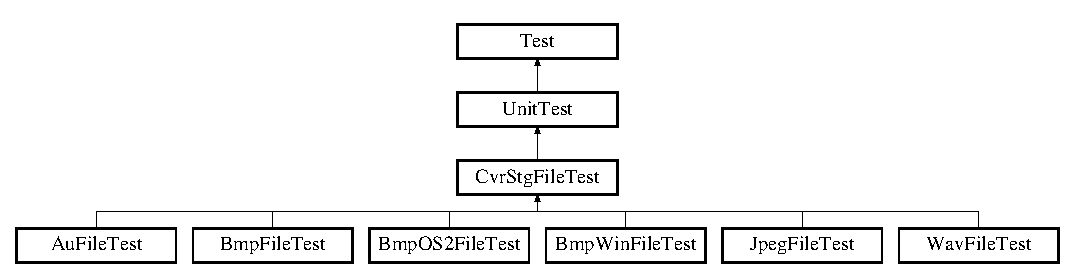
\includegraphics[height=3.303835cm]{classCvrStgFileTest}
\end{center}
\end{figure}
\subsection*{Public Member Functions}
\begin{DoxyCompactItemize}
\item 
\textbf{ Cvr\+Stg\+File\+Test} (std\+::string n, \textbf{ Test\+Suite} $\ast$s)
\end{DoxyCompactItemize}
\subsection*{Protected Member Functions}
\begin{DoxyCompactItemize}
\item 
bool \textbf{ generic\+Test\+Read\+Write} (const std\+::string \&rfn, bool new\+\_\+wfn=true) const
\item 
bool \textbf{ generic\+Test\+Read\+Embed\+Extract} (const std\+::string \&fn, \textbf{ Bit\+String} \&emb) const
\item 
bool \textbf{ generic\+Test\+Read\+Extract\+Compare} (const std\+::string \&fn, \textbf{ Bit\+String} \&emb) const
\item 
bool \textbf{ generic\+Test\+Read\+Embed\+Write\+Read\+Extract} (const std\+::string \&cvrfn, \textbf{ Bit\+String} \&emb) const
\item 
bool \textbf{ generic\+Test\+Position} (const \textbf{ Cvr\+Stg\+File} $\ast$f, const \textbf{ Sample\+Pos} pos, \textbf{ Sample\+Value} $\ast$sv\+\_\+r) const
\item 
bool \textbf{ generic\+Test\+S\+V\+A\+L\+Calculation} (const \textbf{ Cvr\+Stg\+File} $\ast$f, const \textbf{ Graph} $\ast$g) const
\item 
bool \textbf{ generic\+Test\+Embedded\+Value} (const \textbf{ Cvr\+Stg\+File} $\ast$f) const
\end{DoxyCompactItemize}
\subsection*{Private Member Functions}
\begin{DoxyCompactItemize}
\item 
bool \textbf{ are\+Equal} (const std\+::string \&fn1, const std\+::string \&fn2) const
\item 
void \textbf{ remove\+File} (const std\+::string \&fn) const
\item 
void \textbf{ copy\+File} (const std\+::string \&src, const std\+::string \&dest) const
\item 
void \textbf{ move\+File} (const std\+::string \&src, const std\+::string \&dest) const
\end{DoxyCompactItemize}


\subsection{Constructor \& Destructor Documentation}
\mbox{\label{classCvrStgFileTest_a490e6158822a3b73b8935becef5a683f}} 
\index{Cvr\+Stg\+File\+Test@{Cvr\+Stg\+File\+Test}!Cvr\+Stg\+File\+Test@{Cvr\+Stg\+File\+Test}}
\index{Cvr\+Stg\+File\+Test@{Cvr\+Stg\+File\+Test}!Cvr\+Stg\+File\+Test@{Cvr\+Stg\+File\+Test}}
\subsubsection{Cvr\+Stg\+File\+Test()}
{\footnotesize\ttfamily Cvr\+Stg\+File\+Test\+::\+Cvr\+Stg\+File\+Test (\begin{DoxyParamCaption}\item[{std\+::string}]{n,  }\item[{\textbf{ Test\+Suite} $\ast$}]{s }\end{DoxyParamCaption})\hspace{0.3cm}{\ttfamily [inline]}}



\subsection{Member Function Documentation}
\mbox{\label{classCvrStgFileTest_ade841ab9117d084ca19bbeb2562912ab}} 
\index{Cvr\+Stg\+File\+Test@{Cvr\+Stg\+File\+Test}!are\+Equal@{are\+Equal}}
\index{are\+Equal@{are\+Equal}!Cvr\+Stg\+File\+Test@{Cvr\+Stg\+File\+Test}}
\subsubsection{are\+Equal()}
{\footnotesize\ttfamily bool Cvr\+Stg\+File\+Test\+::are\+Equal (\begin{DoxyParamCaption}\item[{const std\+::string \&}]{fn1,  }\item[{const std\+::string \&}]{fn2 }\end{DoxyParamCaption}) const\hspace{0.3cm}{\ttfamily [private]}}

\mbox{\label{classCvrStgFileTest_aef89dd9e7d6208d697d5e7fb3dc3623c}} 
\index{Cvr\+Stg\+File\+Test@{Cvr\+Stg\+File\+Test}!copy\+File@{copy\+File}}
\index{copy\+File@{copy\+File}!Cvr\+Stg\+File\+Test@{Cvr\+Stg\+File\+Test}}
\subsubsection{copy\+File()}
{\footnotesize\ttfamily void Cvr\+Stg\+File\+Test\+::copy\+File (\begin{DoxyParamCaption}\item[{const std\+::string \&}]{src,  }\item[{const std\+::string \&}]{dest }\end{DoxyParamCaption}) const\hspace{0.3cm}{\ttfamily [private]}}

\mbox{\label{classCvrStgFileTest_aafd2079227474a72c9403d9a57ce3d72}} 
\index{Cvr\+Stg\+File\+Test@{Cvr\+Stg\+File\+Test}!generic\+Test\+Embedded\+Value@{generic\+Test\+Embedded\+Value}}
\index{generic\+Test\+Embedded\+Value@{generic\+Test\+Embedded\+Value}!Cvr\+Stg\+File\+Test@{Cvr\+Stg\+File\+Test}}
\subsubsection{generic\+Test\+Embedded\+Value()}
{\footnotesize\ttfamily bool Cvr\+Stg\+File\+Test\+::generic\+Test\+Embedded\+Value (\begin{DoxyParamCaption}\item[{const \textbf{ Cvr\+Stg\+File} $\ast$}]{f }\end{DoxyParamCaption}) const\hspace{0.3cm}{\ttfamily [protected]}}

for all sample positions, test if f-\/$>$get\+Embedded\+Value(p) and f-\/$>$get\+Sample\+Value(p)-\/$>$get\+Embedded\+Value() return the same result \mbox{\label{classCvrStgFileTest_a899e3867e522c92df9bffc39ae2f3f8a}} 
\index{Cvr\+Stg\+File\+Test@{Cvr\+Stg\+File\+Test}!generic\+Test\+Position@{generic\+Test\+Position}}
\index{generic\+Test\+Position@{generic\+Test\+Position}!Cvr\+Stg\+File\+Test@{Cvr\+Stg\+File\+Test}}
\subsubsection{generic\+Test\+Position()}
{\footnotesize\ttfamily bool Cvr\+Stg\+File\+Test\+::generic\+Test\+Position (\begin{DoxyParamCaption}\item[{const \textbf{ Cvr\+Stg\+File} $\ast$}]{f,  }\item[{const \textbf{ Sample\+Pos}}]{pos,  }\item[{\textbf{ Sample\+Value} $\ast$}]{sv\+\_\+r }\end{DoxyParamCaption}) const\hspace{0.3cm}{\ttfamily [protected]}}

\mbox{\label{classCvrStgFileTest_a374274d31964bacded40cb741e70cf92}} 
\index{Cvr\+Stg\+File\+Test@{Cvr\+Stg\+File\+Test}!generic\+Test\+Read\+Embed\+Extract@{generic\+Test\+Read\+Embed\+Extract}}
\index{generic\+Test\+Read\+Embed\+Extract@{generic\+Test\+Read\+Embed\+Extract}!Cvr\+Stg\+File\+Test@{Cvr\+Stg\+File\+Test}}
\subsubsection{generic\+Test\+Read\+Embed\+Extract()}
{\footnotesize\ttfamily bool Cvr\+Stg\+File\+Test\+::generic\+Test\+Read\+Embed\+Extract (\begin{DoxyParamCaption}\item[{const std\+::string \&}]{fn,  }\item[{\textbf{ Bit\+String} \&}]{emb }\end{DoxyParamCaption}) const\hspace{0.3cm}{\ttfamily [protected]}}

\mbox{\label{classCvrStgFileTest_a800a6c6b931f2a6cc6e6994bbebf437c}} 
\index{Cvr\+Stg\+File\+Test@{Cvr\+Stg\+File\+Test}!generic\+Test\+Read\+Embed\+Write\+Read\+Extract@{generic\+Test\+Read\+Embed\+Write\+Read\+Extract}}
\index{generic\+Test\+Read\+Embed\+Write\+Read\+Extract@{generic\+Test\+Read\+Embed\+Write\+Read\+Extract}!Cvr\+Stg\+File\+Test@{Cvr\+Stg\+File\+Test}}
\subsubsection{generic\+Test\+Read\+Embed\+Write\+Read\+Extract()}
{\footnotesize\ttfamily bool Cvr\+Stg\+File\+Test\+::generic\+Test\+Read\+Embed\+Write\+Read\+Extract (\begin{DoxyParamCaption}\item[{const std\+::string \&}]{cvrfn,  }\item[{\textbf{ Bit\+String} \&}]{emb }\end{DoxyParamCaption}) const\hspace{0.3cm}{\ttfamily [protected]}}

\mbox{\label{classCvrStgFileTest_a1be5e78e6b8743fcd52621d6404a9b60}} 
\index{Cvr\+Stg\+File\+Test@{Cvr\+Stg\+File\+Test}!generic\+Test\+Read\+Extract\+Compare@{generic\+Test\+Read\+Extract\+Compare}}
\index{generic\+Test\+Read\+Extract\+Compare@{generic\+Test\+Read\+Extract\+Compare}!Cvr\+Stg\+File\+Test@{Cvr\+Stg\+File\+Test}}
\subsubsection{generic\+Test\+Read\+Extract\+Compare()}
{\footnotesize\ttfamily bool Cvr\+Stg\+File\+Test\+::generic\+Test\+Read\+Extract\+Compare (\begin{DoxyParamCaption}\item[{const std\+::string \&}]{fn,  }\item[{\textbf{ Bit\+String} \&}]{emb }\end{DoxyParamCaption}) const\hspace{0.3cm}{\ttfamily [protected]}}

read fn and extract the first emb.\+get\+Length() bits, return true iff these equal emb \mbox{\label{classCvrStgFileTest_adde58709938e4f73f988d9f631b13723}} 
\index{Cvr\+Stg\+File\+Test@{Cvr\+Stg\+File\+Test}!generic\+Test\+Read\+Write@{generic\+Test\+Read\+Write}}
\index{generic\+Test\+Read\+Write@{generic\+Test\+Read\+Write}!Cvr\+Stg\+File\+Test@{Cvr\+Stg\+File\+Test}}
\subsubsection{generic\+Test\+Read\+Write()}
{\footnotesize\ttfamily bool Cvr\+Stg\+File\+Test\+::generic\+Test\+Read\+Write (\begin{DoxyParamCaption}\item[{const std\+::string \&}]{rfn,  }\item[{bool}]{new\+\_\+wfn = {\ttfamily true} }\end{DoxyParamCaption}) const\hspace{0.3cm}{\ttfamily [protected]}}

read the file rfn and write it again, return true iff write op created what was read by read op 
\begin{DoxyParams}{Parameters}
{\em rfn} & the file name of the file to read \\
\hline
{\em new\+\_\+wfn} & wether to write the data to another file or to rfn (a backup copy is done) \\
\hline
\end{DoxyParams}
\mbox{\label{classCvrStgFileTest_a0be3c1772b798e99c963d1b99150409e}} 
\index{Cvr\+Stg\+File\+Test@{Cvr\+Stg\+File\+Test}!generic\+Test\+S\+V\+A\+L\+Calculation@{generic\+Test\+S\+V\+A\+L\+Calculation}}
\index{generic\+Test\+S\+V\+A\+L\+Calculation@{generic\+Test\+S\+V\+A\+L\+Calculation}!Cvr\+Stg\+File\+Test@{Cvr\+Stg\+File\+Test}}
\subsubsection{generic\+Test\+S\+V\+A\+L\+Calculation()}
{\footnotesize\ttfamily bool Cvr\+Stg\+File\+Test\+::generic\+Test\+S\+V\+A\+L\+Calculation (\begin{DoxyParamCaption}\item[{const \textbf{ Cvr\+Stg\+File} $\ast$}]{f,  }\item[{const \textbf{ Graph} $\ast$}]{g }\end{DoxyParamCaption}) const\hspace{0.3cm}{\ttfamily [protected]}}

\mbox{\label{classCvrStgFileTest_a94f814539db17c02ac3e4f70a3cd96eb}} 
\index{Cvr\+Stg\+File\+Test@{Cvr\+Stg\+File\+Test}!move\+File@{move\+File}}
\index{move\+File@{move\+File}!Cvr\+Stg\+File\+Test@{Cvr\+Stg\+File\+Test}}
\subsubsection{move\+File()}
{\footnotesize\ttfamily void Cvr\+Stg\+File\+Test\+::move\+File (\begin{DoxyParamCaption}\item[{const std\+::string \&}]{src,  }\item[{const std\+::string \&}]{dest }\end{DoxyParamCaption}) const\hspace{0.3cm}{\ttfamily [private]}}

\mbox{\label{classCvrStgFileTest_a20f92774fcd716209a45731a6b977f52}} 
\index{Cvr\+Stg\+File\+Test@{Cvr\+Stg\+File\+Test}!remove\+File@{remove\+File}}
\index{remove\+File@{remove\+File}!Cvr\+Stg\+File\+Test@{Cvr\+Stg\+File\+Test}}
\subsubsection{remove\+File()}
{\footnotesize\ttfamily void Cvr\+Stg\+File\+Test\+::remove\+File (\begin{DoxyParamCaption}\item[{const std\+::string \&}]{fn }\end{DoxyParamCaption}) const\hspace{0.3cm}{\ttfamily [private]}}



The documentation for this class was generated from the following files\+:\begin{DoxyCompactItemize}
\item 
\textbf{ Cvr\+Stg\+File\+Test.\+h}\item 
\textbf{ Cvr\+Stg\+File\+Test.\+cc}\end{DoxyCompactItemize}

\section{Cvr\+Stg\+Object Class Reference}
\label{classCvrStgObject}\index{Cvr\+Stg\+Object@{Cvr\+Stg\+Object}}


an object that can hold embedded data  




{\ttfamily \#include $<$Cvr\+Stg\+Object.\+h$>$}

Inheritance diagram for Cvr\+Stg\+Object\+:\begin{figure}[H]
\begin{center}
\leavevmode
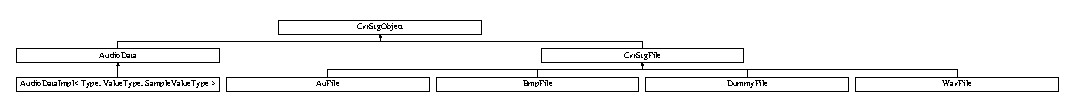
\includegraphics[height=1.005988cm]{classCvrStgObject}
\end{center}
\end{figure}
\subsection*{Public Member Functions}
\begin{DoxyCompactItemize}
\item 
virtual unsigned long \textbf{ get\+Num\+Samples} (void) const =0
\item 
virtual \textbf{ Sample\+Value} $\ast$ \textbf{ get\+Sample\+Value} (const \textbf{ Sample\+Pos} pos) const =0
\item 
virtual void \textbf{ replace\+Sample} (const \textbf{ Sample\+Pos} pos, const \textbf{ Sample\+Value} $\ast$s)=0
\end{DoxyCompactItemize}


\subsection{Detailed Description}
This abstract base class provides an interface for every class that is able to hold embedded data. Something that can hold embedded data is essentially though of as an array of samples.

Definitions\+: Embedded Bit...a bit to be embedded (one bit in the original or extracted embfile) Sample...the smallest data unit in a file (e.\+g. a R\+GB triple, a D\+CT coefficient) 

\subsection{Member Function Documentation}
\mbox{\label{classCvrStgObject_a80ae8f095b66683e5207adf8ff8265b4}} 
\index{Cvr\+Stg\+Object@{Cvr\+Stg\+Object}!get\+Num\+Samples@{get\+Num\+Samples}}
\index{get\+Num\+Samples@{get\+Num\+Samples}!Cvr\+Stg\+Object@{Cvr\+Stg\+Object}}
\subsubsection{get\+Num\+Samples()}
{\footnotesize\ttfamily virtual unsigned long Cvr\+Stg\+Object\+::get\+Num\+Samples (\begin{DoxyParamCaption}\item[{void}]{ }\end{DoxyParamCaption}) const\hspace{0.3cm}{\ttfamily [pure virtual]}}

get the number of samples in this \doxyref{Cvr\+Stg\+Object}{p.}{classCvrStgObject} 

Implemented in \textbf{ Audio\+Data\+Impl$<$ Type, Value\+Type, Sample\+Value\+Type $>$} \doxyref{}{p.}{classAudioDataImpl_a84f684e5b78a19e9b9ecfc530589706a}, \textbf{ Dummy\+File} \doxyref{}{p.}{classDummyFile_a79290dd8bd87a2fabf01f8453d4ce9f0}, \textbf{ Au\+File} \doxyref{}{p.}{classAuFile_a6207c3612049d7467805842de926934e}, \textbf{ Wav\+File} \doxyref{}{p.}{classWavFile_a3345d5c3be349c5e8a6c276e55c5599c}, and \textbf{ Bmp\+File} \doxyref{}{p.}{classBmpFile_a564fb90235f06c80162b9086dcc6e78d}.

\mbox{\label{classCvrStgObject_ac77a8da85a4f7b53e2166e990dfaa4f2}} 
\index{Cvr\+Stg\+Object@{Cvr\+Stg\+Object}!get\+Sample\+Value@{get\+Sample\+Value}}
\index{get\+Sample\+Value@{get\+Sample\+Value}!Cvr\+Stg\+Object@{Cvr\+Stg\+Object}}
\subsubsection{get\+Sample\+Value()}
{\footnotesize\ttfamily virtual \textbf{ Sample\+Value}$\ast$ Cvr\+Stg\+Object\+::get\+Sample\+Value (\begin{DoxyParamCaption}\item[{const \textbf{ Sample\+Pos}}]{pos }\end{DoxyParamCaption}) const\hspace{0.3cm}{\ttfamily [pure virtual]}}

get the sample at position pos 
\begin{DoxyParams}{Parameters}
{\em pos} & the position of a sample (must be in 0...\doxyref{get\+Num\+Samples()}{p.}{classCvrStgObject_a80ae8f095b66683e5207adf8ff8265b4}-\/1) \\
\hline
\end{DoxyParams}
\begin{DoxyReturn}{Returns}
the sample at the given position
\end{DoxyReturn}
The sample object is created in this function and should be deleted by the caller. The derived class should check the condition(s) given above in its Implementation of this function. 

Implemented in \textbf{ Audio\+Data\+Impl$<$ Type, Value\+Type, Sample\+Value\+Type $>$} \doxyref{}{p.}{classAudioDataImpl_a52990850bb0a8a108108f70f378d9461}, \textbf{ Au\+File} \doxyref{}{p.}{classAuFile_af55279548dc9840e46115f859dbac36d}, \textbf{ Dummy\+File} \doxyref{}{p.}{classDummyFile_a44e79fbed4d236321e47d47a9e916e29}, \textbf{ Wav\+File} \doxyref{}{p.}{classWavFile_a64ce0e228da04c36d423dce2f8c6b49a}, and \textbf{ Bmp\+File} \doxyref{}{p.}{classBmpFile_a8a982a74d9d5ef1a33228859e51c888b}.

\mbox{\label{classCvrStgObject_a3068d6a9dcc1c0b8bde2f081cfde6ce5}} 
\index{Cvr\+Stg\+Object@{Cvr\+Stg\+Object}!replace\+Sample@{replace\+Sample}}
\index{replace\+Sample@{replace\+Sample}!Cvr\+Stg\+Object@{Cvr\+Stg\+Object}}
\subsubsection{replace\+Sample()}
{\footnotesize\ttfamily virtual void Cvr\+Stg\+Object\+::replace\+Sample (\begin{DoxyParamCaption}\item[{const \textbf{ Sample\+Pos}}]{pos,  }\item[{const \textbf{ Sample\+Value} $\ast$}]{s }\end{DoxyParamCaption})\hspace{0.3cm}{\ttfamily [pure virtual]}}

replace a sample thus (possibly) altering the value of the bit returned by Sample\+Value-\/$>$get\+Bit() 
\begin{DoxyParams}{Parameters}
{\em pos} & the position of the sample (must be in 0...\doxyref{get\+Num\+Samples()}{p.}{classCvrStgObject_a80ae8f095b66683e5207adf8ff8265b4}-\/1) \\
\hline
{\em s} & the sample value that should replace the current sample value (must be of correct type for this \doxyref{Cvr\+Stg\+Object}{p.}{classCvrStgObject})\\
\hline
\end{DoxyParams}
The derived class should check the condition(s) given above in its Implementation of this function. 

Implemented in \textbf{ Audio\+Data\+Impl$<$ Type, Value\+Type, Sample\+Value\+Type $>$} \doxyref{}{p.}{classAudioDataImpl_a2522e8ff1588325b0fe93210a3c048f5}, \textbf{ Au\+File} \doxyref{}{p.}{classAuFile_a174651b1eb09ce6499dd9b49740e0585}, \textbf{ Dummy\+File} \doxyref{}{p.}{classDummyFile_a702ca13d4515e719785b6c7b670354bb}, \textbf{ Wav\+File} \doxyref{}{p.}{classWavFile_ae73ef41e61806392a53385065ec7e444}, and \textbf{ Bmp\+File} \doxyref{}{p.}{classBmpFile_a9f476c72483674452cf272f9e10d1087}.



The documentation for this class was generated from the following file\+:\begin{DoxyCompactItemize}
\item 
\textbf{ Cvr\+Stg\+Object.\+h}\end{DoxyCompactItemize}

\section{D\+F\+S\+A\+P\+Heuristic Class Reference}
\label{classDFSAPHeuristic}\index{D\+F\+S\+A\+P\+Heuristic@{D\+F\+S\+A\+P\+Heuristic}}


a matching algorithm implementing a heuristic search for augmenting paths  




{\ttfamily \#include $<$D\+F\+S\+A\+P\+Heuristic.\+h$>$}

Inheritance diagram for D\+F\+S\+A\+P\+Heuristic\+:\begin{figure}[H]
\begin{center}
\leavevmode
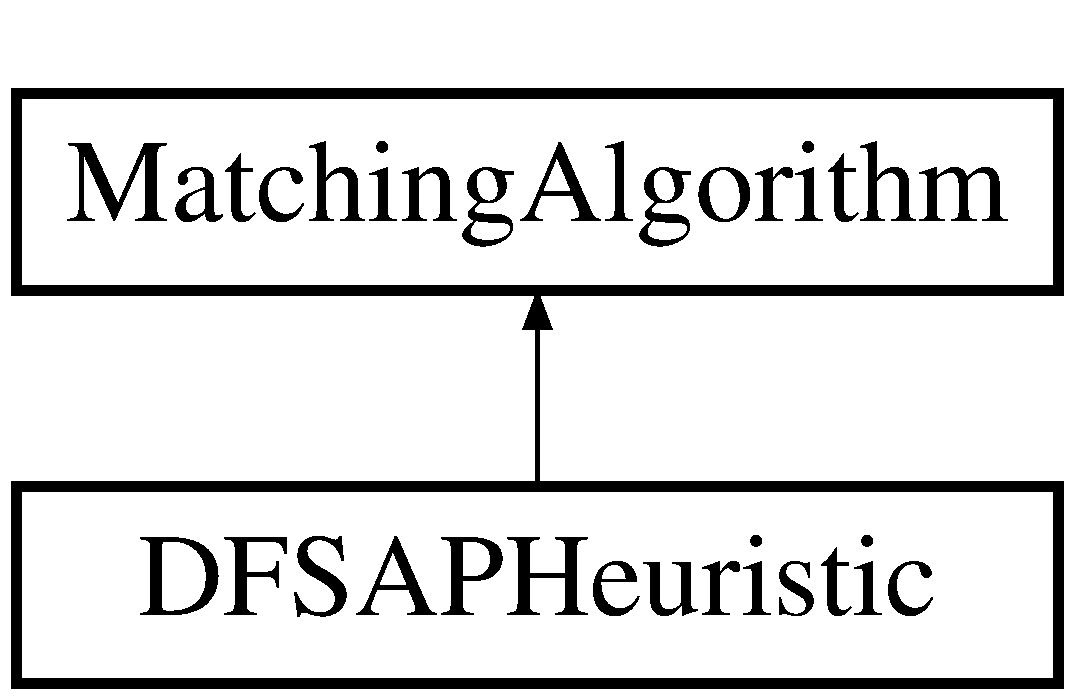
\includegraphics[height=2.000000cm]{classDFSAPHeuristic}
\end{center}
\end{figure}
\subsection*{Public Member Functions}
\begin{DoxyCompactItemize}
\item 
\textbf{ D\+F\+S\+A\+P\+Heuristic} (\textbf{ Graph} $\ast$g, \textbf{ Matching} $\ast$m, float goal=100.\+0, \textbf{ U\+W\+O\+R\+D32} mne=\textbf{ U\+W\+O\+R\+D32\+\_\+\+M\+AX}, \textbf{ Edge\+Iterator\+::\+I\+T\+E\+R\+A\+T\+I\+O\+N\+M\+O\+DE} mo=\textbf{ Edge\+Iterator\+::\+S\+A\+M\+P\+L\+E\+O\+C\+C\+U\+R\+E\+N\+CE})
\item 
virtual \textbf{ $\sim$\+D\+F\+S\+A\+P\+Heuristic} (void)
\item 
const char $\ast$ \textbf{ get\+Name} (void) const
\item 
void \textbf{ reset} (\textbf{ U\+W\+O\+R\+D32} mne=\textbf{ U\+W\+O\+R\+D32\+\_\+\+M\+AX}, \textbf{ Edge\+Iterator\+::\+I\+T\+E\+R\+A\+T\+I\+O\+N\+M\+O\+DE} mo=\textbf{ Edge\+Iterator\+::\+S\+A\+M\+P\+L\+E\+O\+C\+C\+U\+R\+E\+N\+CE})
\item 
void \textbf{ run} (void)
\end{DoxyCompactItemize}
\subsection*{Private Member Functions}
\begin{DoxyCompactItemize}
\item 
unsigned long \textbf{ search\+Augmenting\+Path} (\textbf{ Vertex} $\ast$v0, const \textbf{ Edge} $\ast$$\ast$path)
\item 
const \textbf{ Edge} $\ast$ \textbf{ get\+Next\+Edge} (\textbf{ Vertex} $\ast$v)
\item 
void \textbf{ mark\+Visited} (\textbf{ Vertex} $\ast$v)
\item 
bool \textbf{ is\+Visited} (\textbf{ Vertex} $\ast$v) const
\item 
bool \textbf{ is\+Visited} (\textbf{ Vertex\+Label} vlbl) const
\end{DoxyCompactItemize}
\subsection*{Private Attributes}
\begin{DoxyCompactItemize}
\item 
\textbf{ U\+W\+O\+R\+D32} \textbf{ Time\+Counter}
\item 
\textbf{ U\+W\+O\+R\+D32} $\ast$ \textbf{ Time\+Counters}
\item 
bool $\ast$ \textbf{ Vertex\+On\+Path}
\item 
\textbf{ Edge\+Iterator} $\ast$ \textbf{ Edge\+Iterators}
\end{DoxyCompactItemize}
\subsection*{Additional Inherited Members}


\subsection{Detailed Description}
This class implements the heuristic augmenting path search presented by Rolf H. Moehring and Matthias Mueller-\/\+Hannemann in their paper\+: \char`\"{}\+Cardinality
\+Matching\+: Heuristic Search for Augmenting Paths\char`\"{}. 

\subsection{Constructor \& Destructor Documentation}
\mbox{\label{classDFSAPHeuristic_ab0d70281dd13170430076bb6bf7e6d9d}} 
\index{D\+F\+S\+A\+P\+Heuristic@{D\+F\+S\+A\+P\+Heuristic}!D\+F\+S\+A\+P\+Heuristic@{D\+F\+S\+A\+P\+Heuristic}}
\index{D\+F\+S\+A\+P\+Heuristic@{D\+F\+S\+A\+P\+Heuristic}!D\+F\+S\+A\+P\+Heuristic@{D\+F\+S\+A\+P\+Heuristic}}
\subsubsection{D\+F\+S\+A\+P\+Heuristic()}
{\footnotesize\ttfamily D\+F\+S\+A\+P\+Heuristic\+::\+D\+F\+S\+A\+P\+Heuristic (\begin{DoxyParamCaption}\item[{\textbf{ Graph} $\ast$}]{g,  }\item[{\textbf{ Matching} $\ast$}]{m,  }\item[{float}]{goal = {\ttfamily 100.0},  }\item[{\textbf{ U\+W\+O\+R\+D32}}]{mne = {\ttfamily \textbf{ U\+W\+O\+R\+D32\+\_\+\+M\+AX}},  }\item[{\textbf{ Edge\+Iterator\+::\+I\+T\+E\+R\+A\+T\+I\+O\+N\+M\+O\+DE}}]{mo = {\ttfamily \textbf{ Edge\+Iterator\+::\+S\+A\+M\+P\+L\+E\+O\+C\+C\+U\+R\+E\+N\+CE}} }\end{DoxyParamCaption})}

construct an \doxyref{D\+F\+S\+A\+P\+Heuristic}{p.}{classDFSAPHeuristic} object 
\begin{DoxyParams}{Parameters}
{\em g} & the graph on which this heuristic should run \\
\hline
{\em m} & the matching to start with \\
\hline
{\em goal} & the percentage of matched vertices that should be reached \\
\hline
{\em mne} & the maximum number of edges that should be considered for every vertex \\
\hline
{\em mo} & the mode for edge iteration \\
\hline
\end{DoxyParams}
\mbox{\label{classDFSAPHeuristic_a995ea2e59f6b27143da1efa3799c68f4}} 
\index{D\+F\+S\+A\+P\+Heuristic@{D\+F\+S\+A\+P\+Heuristic}!````~D\+F\+S\+A\+P\+Heuristic@{$\sim$\+D\+F\+S\+A\+P\+Heuristic}}
\index{````~D\+F\+S\+A\+P\+Heuristic@{$\sim$\+D\+F\+S\+A\+P\+Heuristic}!D\+F\+S\+A\+P\+Heuristic@{D\+F\+S\+A\+P\+Heuristic}}
\subsubsection{$\sim$\+D\+F\+S\+A\+P\+Heuristic()}
{\footnotesize\ttfamily D\+F\+S\+A\+P\+Heuristic\+::$\sim$\+D\+F\+S\+A\+P\+Heuristic (\begin{DoxyParamCaption}\item[{void}]{ }\end{DoxyParamCaption})\hspace{0.3cm}{\ttfamily [virtual]}}



\subsection{Member Function Documentation}
\mbox{\label{classDFSAPHeuristic_afd3814466a9968e66558451ae0a0c611}} 
\index{D\+F\+S\+A\+P\+Heuristic@{D\+F\+S\+A\+P\+Heuristic}!get\+Name@{get\+Name}}
\index{get\+Name@{get\+Name}!D\+F\+S\+A\+P\+Heuristic@{D\+F\+S\+A\+P\+Heuristic}}
\subsubsection{get\+Name()}
{\footnotesize\ttfamily const char$\ast$ D\+F\+S\+A\+P\+Heuristic\+::get\+Name (\begin{DoxyParamCaption}\item[{void}]{ }\end{DoxyParamCaption}) const\hspace{0.3cm}{\ttfamily [inline]}, {\ttfamily [virtual]}}



Implements \textbf{ Matching\+Algorithm} \doxyref{}{p.}{classMatchingAlgorithm_a7305edae5d74e91987bcf983b2a1171a}.

\mbox{\label{classDFSAPHeuristic_a8fbae63f1ab832aacf5c432e1270589e}} 
\index{D\+F\+S\+A\+P\+Heuristic@{D\+F\+S\+A\+P\+Heuristic}!get\+Next\+Edge@{get\+Next\+Edge}}
\index{get\+Next\+Edge@{get\+Next\+Edge}!D\+F\+S\+A\+P\+Heuristic@{D\+F\+S\+A\+P\+Heuristic}}
\subsubsection{get\+Next\+Edge()}
{\footnotesize\ttfamily const \textbf{ Edge} $\ast$ D\+F\+S\+A\+P\+Heuristic\+::get\+Next\+Edge (\begin{DoxyParamCaption}\item[{\textbf{ Vertex} $\ast$}]{v }\end{DoxyParamCaption})\hspace{0.3cm}{\ttfamily [private]}}

\mbox{\label{classDFSAPHeuristic_ac1c192383aba7c0ad8035bb0458825bd}} 
\index{D\+F\+S\+A\+P\+Heuristic@{D\+F\+S\+A\+P\+Heuristic}!is\+Visited@{is\+Visited}}
\index{is\+Visited@{is\+Visited}!D\+F\+S\+A\+P\+Heuristic@{D\+F\+S\+A\+P\+Heuristic}}
\subsubsection{is\+Visited()\hspace{0.1cm}{\footnotesize\ttfamily [1/2]}}
{\footnotesize\ttfamily bool D\+F\+S\+A\+P\+Heuristic\+::is\+Visited (\begin{DoxyParamCaption}\item[{\textbf{ Vertex} $\ast$}]{v }\end{DoxyParamCaption}) const\hspace{0.3cm}{\ttfamily [inline]}, {\ttfamily [private]}}

returns true iff v has already been visited in this iteration, i.\+e. in the current call of search\+Augmenting\+Path \mbox{\label{classDFSAPHeuristic_a6aa7765a5171a9947dfbc7d5ab86ed21}} 
\index{D\+F\+S\+A\+P\+Heuristic@{D\+F\+S\+A\+P\+Heuristic}!is\+Visited@{is\+Visited}}
\index{is\+Visited@{is\+Visited}!D\+F\+S\+A\+P\+Heuristic@{D\+F\+S\+A\+P\+Heuristic}}
\subsubsection{is\+Visited()\hspace{0.1cm}{\footnotesize\ttfamily [2/2]}}
{\footnotesize\ttfamily bool D\+F\+S\+A\+P\+Heuristic\+::is\+Visited (\begin{DoxyParamCaption}\item[{\textbf{ Vertex\+Label}}]{vlbl }\end{DoxyParamCaption}) const\hspace{0.3cm}{\ttfamily [inline]}, {\ttfamily [private]}}

\mbox{\label{classDFSAPHeuristic_a88358a5e013978a2211d6cc94cbc19e8}} 
\index{D\+F\+S\+A\+P\+Heuristic@{D\+F\+S\+A\+P\+Heuristic}!mark\+Visited@{mark\+Visited}}
\index{mark\+Visited@{mark\+Visited}!D\+F\+S\+A\+P\+Heuristic@{D\+F\+S\+A\+P\+Heuristic}}
\subsubsection{mark\+Visited()}
{\footnotesize\ttfamily void D\+F\+S\+A\+P\+Heuristic\+::mark\+Visited (\begin{DoxyParamCaption}\item[{\textbf{ Vertex} $\ast$}]{v }\end{DoxyParamCaption})\hspace{0.3cm}{\ttfamily [inline]}, {\ttfamily [private]}}

\mbox{\label{classDFSAPHeuristic_aa32cf73dfea46c56170ab93d038aa1bb}} 
\index{D\+F\+S\+A\+P\+Heuristic@{D\+F\+S\+A\+P\+Heuristic}!reset@{reset}}
\index{reset@{reset}!D\+F\+S\+A\+P\+Heuristic@{D\+F\+S\+A\+P\+Heuristic}}
\subsubsection{reset()}
{\footnotesize\ttfamily void D\+F\+S\+A\+P\+Heuristic\+::reset (\begin{DoxyParamCaption}\item[{\textbf{ U\+W\+O\+R\+D32}}]{mne = {\ttfamily \textbf{ U\+W\+O\+R\+D32\+\_\+\+M\+AX}},  }\item[{\textbf{ Edge\+Iterator\+::\+I\+T\+E\+R\+A\+T\+I\+O\+N\+M\+O\+DE}}]{mo = {\ttfamily \textbf{ Edge\+Iterator\+::\+S\+A\+M\+P\+L\+E\+O\+C\+C\+U\+R\+E\+N\+CE}} }\end{DoxyParamCaption})}

reset the state of this \doxyref{D\+F\+S\+A\+P\+Heuristic}{p.}{classDFSAPHeuristic}, esp. the Edge\+Iterators 
\begin{DoxyParams}{Parameters}
{\em mne} & the maximum number of edges that should be considered for every vertex for now on \\
\hline
\end{DoxyParams}
\mbox{\label{classDFSAPHeuristic_a6be8de5d724975d145500fc7a1f12198}} 
\index{D\+F\+S\+A\+P\+Heuristic@{D\+F\+S\+A\+P\+Heuristic}!run@{run}}
\index{run@{run}!D\+F\+S\+A\+P\+Heuristic@{D\+F\+S\+A\+P\+Heuristic}}
\subsubsection{run()}
{\footnotesize\ttfamily void D\+F\+S\+A\+P\+Heuristic\+::run (\begin{DoxyParamCaption}\item[{void}]{ }\end{DoxyParamCaption})\hspace{0.3cm}{\ttfamily [virtual]}}



Implements \textbf{ Matching\+Algorithm} \doxyref{}{p.}{classMatchingAlgorithm_aeea6c808daf03fd788c9a9feea885c41}.

\mbox{\label{classDFSAPHeuristic_a2046bacf3bdd3468cd5732bb7544a090}} 
\index{D\+F\+S\+A\+P\+Heuristic@{D\+F\+S\+A\+P\+Heuristic}!search\+Augmenting\+Path@{search\+Augmenting\+Path}}
\index{search\+Augmenting\+Path@{search\+Augmenting\+Path}!D\+F\+S\+A\+P\+Heuristic@{D\+F\+S\+A\+P\+Heuristic}}
\subsubsection{search\+Augmenting\+Path()}
{\footnotesize\ttfamily unsigned long D\+F\+S\+A\+P\+Heuristic\+::search\+Augmenting\+Path (\begin{DoxyParamCaption}\item[{\textbf{ Vertex} $\ast$}]{v0,  }\item[{const \textbf{ Edge} $\ast$$\ast$}]{path }\end{DoxyParamCaption})\hspace{0.3cm}{\ttfamily [private]}}


\begin{DoxyParams}{Parameters}
{\em v0} & an exposed vertex \\
\hline
{\em path} & an array of \doxyref{Edge}{p.}{classEdge} pointers where the path will be put \\
\hline
\end{DoxyParams}
\begin{DoxyReturn}{Returns}
the length of the path (the number of valid edges in path) 
\end{DoxyReturn}


\subsection{Member Data Documentation}
\mbox{\label{classDFSAPHeuristic_aa31f7a99d7771193e274d962c2841a2c}} 
\index{D\+F\+S\+A\+P\+Heuristic@{D\+F\+S\+A\+P\+Heuristic}!Edge\+Iterators@{Edge\+Iterators}}
\index{Edge\+Iterators@{Edge\+Iterators}!D\+F\+S\+A\+P\+Heuristic@{D\+F\+S\+A\+P\+Heuristic}}
\subsubsection{Edge\+Iterators}
{\footnotesize\ttfamily \textbf{ Edge\+Iterator}$\ast$ D\+F\+S\+A\+P\+Heuristic\+::\+Edge\+Iterators\hspace{0.3cm}{\ttfamily [private]}}

\mbox{\label{classDFSAPHeuristic_a58332cda0fbc79a94ff15b2715cdb59e}} 
\index{D\+F\+S\+A\+P\+Heuristic@{D\+F\+S\+A\+P\+Heuristic}!Time\+Counter@{Time\+Counter}}
\index{Time\+Counter@{Time\+Counter}!D\+F\+S\+A\+P\+Heuristic@{D\+F\+S\+A\+P\+Heuristic}}
\subsubsection{Time\+Counter}
{\footnotesize\ttfamily \textbf{ U\+W\+O\+R\+D32} D\+F\+S\+A\+P\+Heuristic\+::\+Time\+Counter\hspace{0.3cm}{\ttfamily [private]}}

\mbox{\label{classDFSAPHeuristic_aef8179c11e9f17f0499281ff4ea04a57}} 
\index{D\+F\+S\+A\+P\+Heuristic@{D\+F\+S\+A\+P\+Heuristic}!Time\+Counters@{Time\+Counters}}
\index{Time\+Counters@{Time\+Counters}!D\+F\+S\+A\+P\+Heuristic@{D\+F\+S\+A\+P\+Heuristic}}
\subsubsection{Time\+Counters}
{\footnotesize\ttfamily \textbf{ U\+W\+O\+R\+D32}$\ast$ D\+F\+S\+A\+P\+Heuristic\+::\+Time\+Counters\hspace{0.3cm}{\ttfamily [private]}}

\mbox{\label{classDFSAPHeuristic_a25fe18d2559609eab338ab4c2fffd9fc}} 
\index{D\+F\+S\+A\+P\+Heuristic@{D\+F\+S\+A\+P\+Heuristic}!Vertex\+On\+Path@{Vertex\+On\+Path}}
\index{Vertex\+On\+Path@{Vertex\+On\+Path}!D\+F\+S\+A\+P\+Heuristic@{D\+F\+S\+A\+P\+Heuristic}}
\subsubsection{Vertex\+On\+Path}
{\footnotesize\ttfamily bool$\ast$ D\+F\+S\+A\+P\+Heuristic\+::\+Vertex\+On\+Path\hspace{0.3cm}{\ttfamily [private]}}



The documentation for this class was generated from the following files\+:\begin{DoxyCompactItemize}
\item 
\textbf{ D\+F\+S\+A\+P\+Heuristic.\+h}\item 
\textbf{ D\+F\+S\+A\+P\+Heuristic.\+cc}\end{DoxyCompactItemize}

\section{D\+F\+S\+A\+P\+Heuristic\+Test Class Reference}
\label{classDFSAPHeuristicTest}\index{D\+F\+S\+A\+P\+Heuristic\+Test@{D\+F\+S\+A\+P\+Heuristic\+Test}}


{\ttfamily \#include $<$D\+F\+S\+A\+P\+Heuristic\+Test.\+h$>$}

Inheritance diagram for D\+F\+S\+A\+P\+Heuristic\+Test\+:\begin{figure}[H]
\begin{center}
\leavevmode
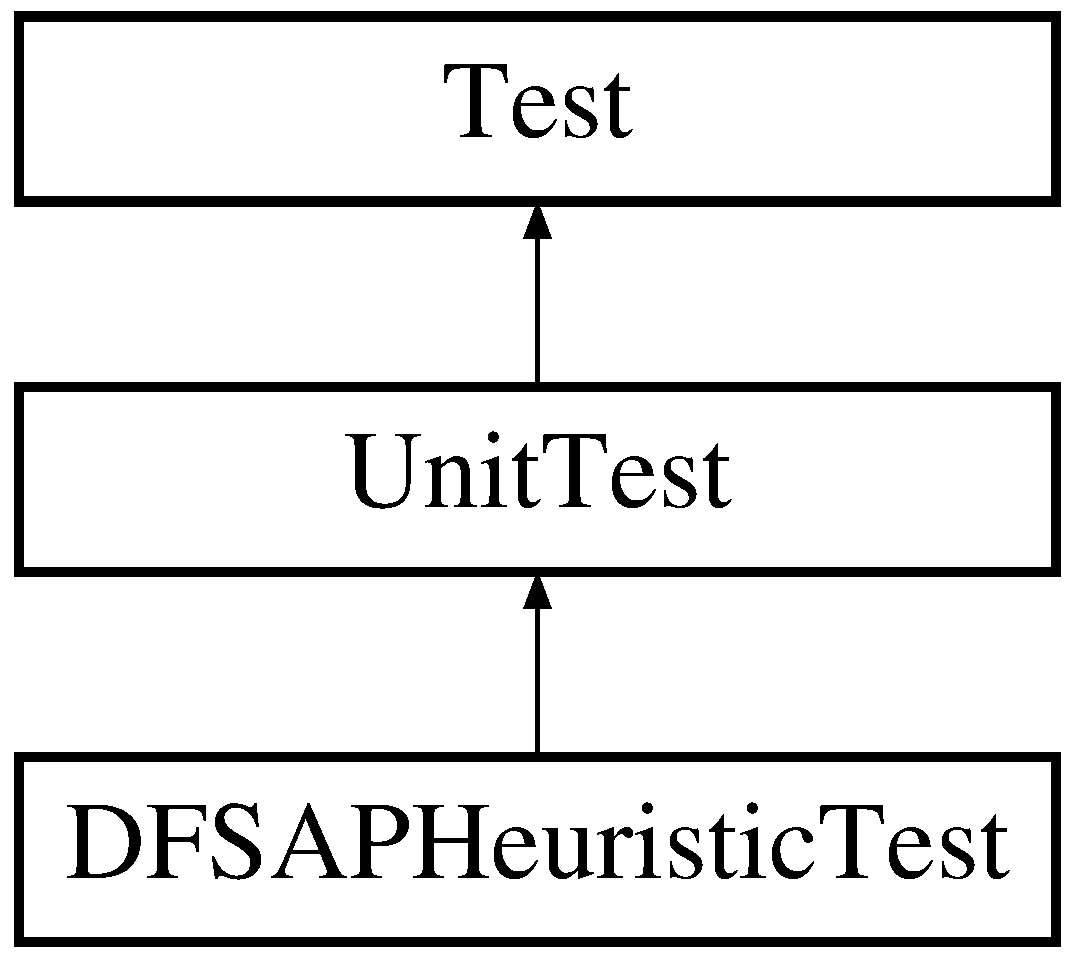
\includegraphics[height=3.000000cm]{classDFSAPHeuristicTest}
\end{center}
\end{figure}
\subsection*{Public Member Functions}
\begin{DoxyCompactItemize}
\item 
\textbf{ D\+F\+S\+A\+P\+Heuristic\+Test} (\textbf{ Test\+Suite} $\ast$s)
\item 
void \textbf{ setup} (void)
\item 
void \textbf{ cleanup} (void)
\item 
void \textbf{ test\+Algorithm} (void)
\end{DoxyCompactItemize}
\subsection*{Private Attributes}
\begin{DoxyCompactItemize}
\item 
\textbf{ Bit\+String} $\ast$ \textbf{ bs1}
\item 
\textbf{ Bit\+String} $\ast$ \textbf{ bs2}
\item 
\textbf{ Bit\+String} $\ast$ \textbf{ bs3}
\item 
\textbf{ Bit\+String} $\ast$ \textbf{ bs4}
\item 
\textbf{ Bit\+String} $\ast$ \textbf{ bs5}
\item 
\textbf{ Cvr\+Stg\+File} $\ast$ \textbf{ f1}
\item 
\textbf{ Cvr\+Stg\+File} $\ast$ \textbf{ f2}
\item 
\textbf{ Cvr\+Stg\+File} $\ast$ \textbf{ f3}
\item 
\textbf{ Cvr\+Stg\+File} $\ast$ \textbf{ f4}
\item 
\textbf{ Cvr\+Stg\+File} $\ast$ \textbf{ f5}
\item 
\textbf{ Selector} $\ast$ \textbf{ s1}
\item 
\textbf{ Selector} $\ast$ \textbf{ s2}
\item 
\textbf{ Selector} $\ast$ \textbf{ s3}
\item 
\textbf{ Selector} $\ast$ \textbf{ s4}
\item 
\textbf{ Selector} $\ast$ \textbf{ s5}
\item 
\textbf{ Graph} $\ast$ \textbf{ g1}
\item 
\textbf{ Graph} $\ast$ \textbf{ g2}
\item 
\textbf{ Graph} $\ast$ \textbf{ g3}
\item 
\textbf{ Graph} $\ast$ \textbf{ g4}
\item 
\textbf{ Graph} $\ast$ \textbf{ g5}
\item 
\textbf{ Matching} $\ast$ \textbf{ m1}
\item 
\textbf{ Matching} $\ast$ \textbf{ m2}
\item 
\textbf{ Matching} $\ast$ \textbf{ m3}
\item 
\textbf{ Matching} $\ast$ \textbf{ m4}
\item 
\textbf{ Matching} $\ast$ \textbf{ m5}
\item 
\textbf{ D\+F\+S\+A\+P\+Heuristic} $\ast$ \textbf{ aph1}
\item 
\textbf{ D\+F\+S\+A\+P\+Heuristic} $\ast$ \textbf{ aph2}
\item 
\textbf{ D\+F\+S\+A\+P\+Heuristic} $\ast$ \textbf{ aph3}
\item 
\textbf{ D\+F\+S\+A\+P\+Heuristic} $\ast$ \textbf{ aph4}
\item 
\textbf{ D\+F\+S\+A\+P\+Heuristic} $\ast$ \textbf{ aph5}
\item 
\textbf{ Globals} \textbf{ gl1}
\item 
\textbf{ Globals} \textbf{ gl2}
\item 
\textbf{ Globals} \textbf{ gl3}
\item 
\textbf{ Globals} \textbf{ gl4}
\item 
\textbf{ Globals} \textbf{ gl5}
\end{DoxyCompactItemize}
\subsection*{Additional Inherited Members}


\subsection{Constructor \& Destructor Documentation}
\mbox{\label{classDFSAPHeuristicTest_a0c88853d5a6970d6f44b9b173c1656cc}} 
\index{D\+F\+S\+A\+P\+Heuristic\+Test@{D\+F\+S\+A\+P\+Heuristic\+Test}!D\+F\+S\+A\+P\+Heuristic\+Test@{D\+F\+S\+A\+P\+Heuristic\+Test}}
\index{D\+F\+S\+A\+P\+Heuristic\+Test@{D\+F\+S\+A\+P\+Heuristic\+Test}!D\+F\+S\+A\+P\+Heuristic\+Test@{D\+F\+S\+A\+P\+Heuristic\+Test}}
\subsubsection{D\+F\+S\+A\+P\+Heuristic\+Test()}
{\footnotesize\ttfamily D\+F\+S\+A\+P\+Heuristic\+Test\+::\+D\+F\+S\+A\+P\+Heuristic\+Test (\begin{DoxyParamCaption}\item[{\textbf{ Test\+Suite} $\ast$}]{s }\end{DoxyParamCaption})}



\subsection{Member Function Documentation}
\mbox{\label{classDFSAPHeuristicTest_afab26fa7135d6b59edaaa83aadb60e8c}} 
\index{D\+F\+S\+A\+P\+Heuristic\+Test@{D\+F\+S\+A\+P\+Heuristic\+Test}!cleanup@{cleanup}}
\index{cleanup@{cleanup}!D\+F\+S\+A\+P\+Heuristic\+Test@{D\+F\+S\+A\+P\+Heuristic\+Test}}
\subsubsection{cleanup()}
{\footnotesize\ttfamily void D\+F\+S\+A\+P\+Heuristic\+Test\+::cleanup (\begin{DoxyParamCaption}\item[{void}]{ }\end{DoxyParamCaption})\hspace{0.3cm}{\ttfamily [virtual]}}

cleanup the unit test -\/ called after run 

Reimplemented from \textbf{ Unit\+Test} \doxyref{}{p.}{classUnitTest_adf77efe972ee4a766d94e3f7ddc193ad}.

\mbox{\label{classDFSAPHeuristicTest_a72fb16e54187758148f9e2b18687d5ac}} 
\index{D\+F\+S\+A\+P\+Heuristic\+Test@{D\+F\+S\+A\+P\+Heuristic\+Test}!setup@{setup}}
\index{setup@{setup}!D\+F\+S\+A\+P\+Heuristic\+Test@{D\+F\+S\+A\+P\+Heuristic\+Test}}
\subsubsection{setup()}
{\footnotesize\ttfamily void D\+F\+S\+A\+P\+Heuristic\+Test\+::setup (\begin{DoxyParamCaption}\item[{void}]{ }\end{DoxyParamCaption})\hspace{0.3cm}{\ttfamily [virtual]}}

setup the unit test -\/ called before run

\doxyref{Unit\+Test\+::setup}{p.}{classUnitTest_ad73fdf9012b651047ea001d21f9d27ad} will (together with \doxyref{Unit\+Test\+::cleanup}{p.}{classUnitTest_adf77efe972ee4a766d94e3f7ddc193ad}) save and restore the object stored in Globs so they should be called from the corresponding functions in the derived object if the derived unit test manipulates the Globs object. 

Reimplemented from \textbf{ Unit\+Test} \doxyref{}{p.}{classUnitTest_ad73fdf9012b651047ea001d21f9d27ad}.

\mbox{\label{classDFSAPHeuristicTest_af357c71961ce93f7fac19d15663cab0d}} 
\index{D\+F\+S\+A\+P\+Heuristic\+Test@{D\+F\+S\+A\+P\+Heuristic\+Test}!test\+Algorithm@{test\+Algorithm}}
\index{test\+Algorithm@{test\+Algorithm}!D\+F\+S\+A\+P\+Heuristic\+Test@{D\+F\+S\+A\+P\+Heuristic\+Test}}
\subsubsection{test\+Algorithm()}
{\footnotesize\ttfamily void D\+F\+S\+A\+P\+Heuristic\+Test\+::test\+Algorithm (\begin{DoxyParamCaption}\item[{void}]{ }\end{DoxyParamCaption})}



\subsection{Member Data Documentation}
\mbox{\label{classDFSAPHeuristicTest_a59e5bf3f83027c0d8ca29f4449066201}} 
\index{D\+F\+S\+A\+P\+Heuristic\+Test@{D\+F\+S\+A\+P\+Heuristic\+Test}!aph1@{aph1}}
\index{aph1@{aph1}!D\+F\+S\+A\+P\+Heuristic\+Test@{D\+F\+S\+A\+P\+Heuristic\+Test}}
\subsubsection{aph1}
{\footnotesize\ttfamily \textbf{ D\+F\+S\+A\+P\+Heuristic}$\ast$ D\+F\+S\+A\+P\+Heuristic\+Test\+::aph1\hspace{0.3cm}{\ttfamily [private]}}

\mbox{\label{classDFSAPHeuristicTest_a331faa236ff9ca867700bfa85143fe16}} 
\index{D\+F\+S\+A\+P\+Heuristic\+Test@{D\+F\+S\+A\+P\+Heuristic\+Test}!aph2@{aph2}}
\index{aph2@{aph2}!D\+F\+S\+A\+P\+Heuristic\+Test@{D\+F\+S\+A\+P\+Heuristic\+Test}}
\subsubsection{aph2}
{\footnotesize\ttfamily \textbf{ D\+F\+S\+A\+P\+Heuristic} $\ast$ D\+F\+S\+A\+P\+Heuristic\+Test\+::aph2\hspace{0.3cm}{\ttfamily [private]}}

\mbox{\label{classDFSAPHeuristicTest_ae2d7e723f34c59735e7266c8d0609c57}} 
\index{D\+F\+S\+A\+P\+Heuristic\+Test@{D\+F\+S\+A\+P\+Heuristic\+Test}!aph3@{aph3}}
\index{aph3@{aph3}!D\+F\+S\+A\+P\+Heuristic\+Test@{D\+F\+S\+A\+P\+Heuristic\+Test}}
\subsubsection{aph3}
{\footnotesize\ttfamily \textbf{ D\+F\+S\+A\+P\+Heuristic} $\ast$ D\+F\+S\+A\+P\+Heuristic\+Test\+::aph3\hspace{0.3cm}{\ttfamily [private]}}

\mbox{\label{classDFSAPHeuristicTest_a3bb3b90515559f05916d67f59c2c92a1}} 
\index{D\+F\+S\+A\+P\+Heuristic\+Test@{D\+F\+S\+A\+P\+Heuristic\+Test}!aph4@{aph4}}
\index{aph4@{aph4}!D\+F\+S\+A\+P\+Heuristic\+Test@{D\+F\+S\+A\+P\+Heuristic\+Test}}
\subsubsection{aph4}
{\footnotesize\ttfamily \textbf{ D\+F\+S\+A\+P\+Heuristic} $\ast$ D\+F\+S\+A\+P\+Heuristic\+Test\+::aph4\hspace{0.3cm}{\ttfamily [private]}}

\mbox{\label{classDFSAPHeuristicTest_a314b35dc7e51ccc1dd546c055674f08a}} 
\index{D\+F\+S\+A\+P\+Heuristic\+Test@{D\+F\+S\+A\+P\+Heuristic\+Test}!aph5@{aph5}}
\index{aph5@{aph5}!D\+F\+S\+A\+P\+Heuristic\+Test@{D\+F\+S\+A\+P\+Heuristic\+Test}}
\subsubsection{aph5}
{\footnotesize\ttfamily \textbf{ D\+F\+S\+A\+P\+Heuristic} $\ast$ D\+F\+S\+A\+P\+Heuristic\+Test\+::aph5\hspace{0.3cm}{\ttfamily [private]}}

\mbox{\label{classDFSAPHeuristicTest_a9cb4b8bd67faf3200b3e9f5b5098d261}} 
\index{D\+F\+S\+A\+P\+Heuristic\+Test@{D\+F\+S\+A\+P\+Heuristic\+Test}!bs1@{bs1}}
\index{bs1@{bs1}!D\+F\+S\+A\+P\+Heuristic\+Test@{D\+F\+S\+A\+P\+Heuristic\+Test}}
\subsubsection{bs1}
{\footnotesize\ttfamily \textbf{ Bit\+String}$\ast$ D\+F\+S\+A\+P\+Heuristic\+Test\+::bs1\hspace{0.3cm}{\ttfamily [private]}}

\mbox{\label{classDFSAPHeuristicTest_a9c54dce23421ea72cbb1bfc20ffe01a6}} 
\index{D\+F\+S\+A\+P\+Heuristic\+Test@{D\+F\+S\+A\+P\+Heuristic\+Test}!bs2@{bs2}}
\index{bs2@{bs2}!D\+F\+S\+A\+P\+Heuristic\+Test@{D\+F\+S\+A\+P\+Heuristic\+Test}}
\subsubsection{bs2}
{\footnotesize\ttfamily \textbf{ Bit\+String} $\ast$ D\+F\+S\+A\+P\+Heuristic\+Test\+::bs2\hspace{0.3cm}{\ttfamily [private]}}

\mbox{\label{classDFSAPHeuristicTest_a0b180d8c1402e6a2611de3476f0d4192}} 
\index{D\+F\+S\+A\+P\+Heuristic\+Test@{D\+F\+S\+A\+P\+Heuristic\+Test}!bs3@{bs3}}
\index{bs3@{bs3}!D\+F\+S\+A\+P\+Heuristic\+Test@{D\+F\+S\+A\+P\+Heuristic\+Test}}
\subsubsection{bs3}
{\footnotesize\ttfamily \textbf{ Bit\+String} $\ast$ D\+F\+S\+A\+P\+Heuristic\+Test\+::bs3\hspace{0.3cm}{\ttfamily [private]}}

\mbox{\label{classDFSAPHeuristicTest_ad09dc7433ac3bea7840321913f04e4d6}} 
\index{D\+F\+S\+A\+P\+Heuristic\+Test@{D\+F\+S\+A\+P\+Heuristic\+Test}!bs4@{bs4}}
\index{bs4@{bs4}!D\+F\+S\+A\+P\+Heuristic\+Test@{D\+F\+S\+A\+P\+Heuristic\+Test}}
\subsubsection{bs4}
{\footnotesize\ttfamily \textbf{ Bit\+String} $\ast$ D\+F\+S\+A\+P\+Heuristic\+Test\+::bs4\hspace{0.3cm}{\ttfamily [private]}}

\mbox{\label{classDFSAPHeuristicTest_a54a6b61cb6fedeeab8da72483bfabfe9}} 
\index{D\+F\+S\+A\+P\+Heuristic\+Test@{D\+F\+S\+A\+P\+Heuristic\+Test}!bs5@{bs5}}
\index{bs5@{bs5}!D\+F\+S\+A\+P\+Heuristic\+Test@{D\+F\+S\+A\+P\+Heuristic\+Test}}
\subsubsection{bs5}
{\footnotesize\ttfamily \textbf{ Bit\+String} $\ast$ D\+F\+S\+A\+P\+Heuristic\+Test\+::bs5\hspace{0.3cm}{\ttfamily [private]}}

\mbox{\label{classDFSAPHeuristicTest_ad39016bfec1ddc30a5a8b12547127bb7}} 
\index{D\+F\+S\+A\+P\+Heuristic\+Test@{D\+F\+S\+A\+P\+Heuristic\+Test}!f1@{f1}}
\index{f1@{f1}!D\+F\+S\+A\+P\+Heuristic\+Test@{D\+F\+S\+A\+P\+Heuristic\+Test}}
\subsubsection{f1}
{\footnotesize\ttfamily \textbf{ Cvr\+Stg\+File}$\ast$ D\+F\+S\+A\+P\+Heuristic\+Test\+::f1\hspace{0.3cm}{\ttfamily [private]}}

\mbox{\label{classDFSAPHeuristicTest_ab3c090f1e0fb8cc94ba5aa24e108d911}} 
\index{D\+F\+S\+A\+P\+Heuristic\+Test@{D\+F\+S\+A\+P\+Heuristic\+Test}!f2@{f2}}
\index{f2@{f2}!D\+F\+S\+A\+P\+Heuristic\+Test@{D\+F\+S\+A\+P\+Heuristic\+Test}}
\subsubsection{f2}
{\footnotesize\ttfamily \textbf{ Cvr\+Stg\+File} $\ast$ D\+F\+S\+A\+P\+Heuristic\+Test\+::f2\hspace{0.3cm}{\ttfamily [private]}}

\mbox{\label{classDFSAPHeuristicTest_a4f3bd4adc52c876e27305340f5a767bc}} 
\index{D\+F\+S\+A\+P\+Heuristic\+Test@{D\+F\+S\+A\+P\+Heuristic\+Test}!f3@{f3}}
\index{f3@{f3}!D\+F\+S\+A\+P\+Heuristic\+Test@{D\+F\+S\+A\+P\+Heuristic\+Test}}
\subsubsection{f3}
{\footnotesize\ttfamily \textbf{ Cvr\+Stg\+File} $\ast$ D\+F\+S\+A\+P\+Heuristic\+Test\+::f3\hspace{0.3cm}{\ttfamily [private]}}

\mbox{\label{classDFSAPHeuristicTest_adea9c84cbf1a16e43566b20706e76aa6}} 
\index{D\+F\+S\+A\+P\+Heuristic\+Test@{D\+F\+S\+A\+P\+Heuristic\+Test}!f4@{f4}}
\index{f4@{f4}!D\+F\+S\+A\+P\+Heuristic\+Test@{D\+F\+S\+A\+P\+Heuristic\+Test}}
\subsubsection{f4}
{\footnotesize\ttfamily \textbf{ Cvr\+Stg\+File} $\ast$ D\+F\+S\+A\+P\+Heuristic\+Test\+::f4\hspace{0.3cm}{\ttfamily [private]}}

\mbox{\label{classDFSAPHeuristicTest_a95fc33a20618864c9c6ab3680fde212b}} 
\index{D\+F\+S\+A\+P\+Heuristic\+Test@{D\+F\+S\+A\+P\+Heuristic\+Test}!f5@{f5}}
\index{f5@{f5}!D\+F\+S\+A\+P\+Heuristic\+Test@{D\+F\+S\+A\+P\+Heuristic\+Test}}
\subsubsection{f5}
{\footnotesize\ttfamily \textbf{ Cvr\+Stg\+File} $\ast$ D\+F\+S\+A\+P\+Heuristic\+Test\+::f5\hspace{0.3cm}{\ttfamily [private]}}

\mbox{\label{classDFSAPHeuristicTest_a10c1ef014864145669b3954e051eb11d}} 
\index{D\+F\+S\+A\+P\+Heuristic\+Test@{D\+F\+S\+A\+P\+Heuristic\+Test}!g1@{g1}}
\index{g1@{g1}!D\+F\+S\+A\+P\+Heuristic\+Test@{D\+F\+S\+A\+P\+Heuristic\+Test}}
\subsubsection{g1}
{\footnotesize\ttfamily \textbf{ Graph}$\ast$ D\+F\+S\+A\+P\+Heuristic\+Test\+::g1\hspace{0.3cm}{\ttfamily [private]}}

\mbox{\label{classDFSAPHeuristicTest_af556454fc58bedef72091c54a1d41d4a}} 
\index{D\+F\+S\+A\+P\+Heuristic\+Test@{D\+F\+S\+A\+P\+Heuristic\+Test}!g2@{g2}}
\index{g2@{g2}!D\+F\+S\+A\+P\+Heuristic\+Test@{D\+F\+S\+A\+P\+Heuristic\+Test}}
\subsubsection{g2}
{\footnotesize\ttfamily \textbf{ Graph} $\ast$ D\+F\+S\+A\+P\+Heuristic\+Test\+::g2\hspace{0.3cm}{\ttfamily [private]}}

\mbox{\label{classDFSAPHeuristicTest_aa854b0f32aa95b09a6c58776a0cdb1f7}} 
\index{D\+F\+S\+A\+P\+Heuristic\+Test@{D\+F\+S\+A\+P\+Heuristic\+Test}!g3@{g3}}
\index{g3@{g3}!D\+F\+S\+A\+P\+Heuristic\+Test@{D\+F\+S\+A\+P\+Heuristic\+Test}}
\subsubsection{g3}
{\footnotesize\ttfamily \textbf{ Graph} $\ast$ D\+F\+S\+A\+P\+Heuristic\+Test\+::g3\hspace{0.3cm}{\ttfamily [private]}}

\mbox{\label{classDFSAPHeuristicTest_abd740fc738f2042954e196131c33281b}} 
\index{D\+F\+S\+A\+P\+Heuristic\+Test@{D\+F\+S\+A\+P\+Heuristic\+Test}!g4@{g4}}
\index{g4@{g4}!D\+F\+S\+A\+P\+Heuristic\+Test@{D\+F\+S\+A\+P\+Heuristic\+Test}}
\subsubsection{g4}
{\footnotesize\ttfamily \textbf{ Graph} $\ast$ D\+F\+S\+A\+P\+Heuristic\+Test\+::g4\hspace{0.3cm}{\ttfamily [private]}}

\mbox{\label{classDFSAPHeuristicTest_ad9095b72adfb580a2b5377812299a3d6}} 
\index{D\+F\+S\+A\+P\+Heuristic\+Test@{D\+F\+S\+A\+P\+Heuristic\+Test}!g5@{g5}}
\index{g5@{g5}!D\+F\+S\+A\+P\+Heuristic\+Test@{D\+F\+S\+A\+P\+Heuristic\+Test}}
\subsubsection{g5}
{\footnotesize\ttfamily \textbf{ Graph} $\ast$ D\+F\+S\+A\+P\+Heuristic\+Test\+::g5\hspace{0.3cm}{\ttfamily [private]}}

\mbox{\label{classDFSAPHeuristicTest_a49a5590afbf1d14868129a53ffe6ba57}} 
\index{D\+F\+S\+A\+P\+Heuristic\+Test@{D\+F\+S\+A\+P\+Heuristic\+Test}!gl1@{gl1}}
\index{gl1@{gl1}!D\+F\+S\+A\+P\+Heuristic\+Test@{D\+F\+S\+A\+P\+Heuristic\+Test}}
\subsubsection{gl1}
{\footnotesize\ttfamily \textbf{ Globals} D\+F\+S\+A\+P\+Heuristic\+Test\+::gl1\hspace{0.3cm}{\ttfamily [private]}}

\mbox{\label{classDFSAPHeuristicTest_a782af69af851dd301b86974fdf0363c1}} 
\index{D\+F\+S\+A\+P\+Heuristic\+Test@{D\+F\+S\+A\+P\+Heuristic\+Test}!gl2@{gl2}}
\index{gl2@{gl2}!D\+F\+S\+A\+P\+Heuristic\+Test@{D\+F\+S\+A\+P\+Heuristic\+Test}}
\subsubsection{gl2}
{\footnotesize\ttfamily \textbf{ Globals} D\+F\+S\+A\+P\+Heuristic\+Test\+::gl2\hspace{0.3cm}{\ttfamily [private]}}

\mbox{\label{classDFSAPHeuristicTest_a5ddfc1fd24b051d2e5d789a9146f9023}} 
\index{D\+F\+S\+A\+P\+Heuristic\+Test@{D\+F\+S\+A\+P\+Heuristic\+Test}!gl3@{gl3}}
\index{gl3@{gl3}!D\+F\+S\+A\+P\+Heuristic\+Test@{D\+F\+S\+A\+P\+Heuristic\+Test}}
\subsubsection{gl3}
{\footnotesize\ttfamily \textbf{ Globals} D\+F\+S\+A\+P\+Heuristic\+Test\+::gl3\hspace{0.3cm}{\ttfamily [private]}}

\mbox{\label{classDFSAPHeuristicTest_af11bbf9da5a42d45873e74da308b6296}} 
\index{D\+F\+S\+A\+P\+Heuristic\+Test@{D\+F\+S\+A\+P\+Heuristic\+Test}!gl4@{gl4}}
\index{gl4@{gl4}!D\+F\+S\+A\+P\+Heuristic\+Test@{D\+F\+S\+A\+P\+Heuristic\+Test}}
\subsubsection{gl4}
{\footnotesize\ttfamily \textbf{ Globals} D\+F\+S\+A\+P\+Heuristic\+Test\+::gl4\hspace{0.3cm}{\ttfamily [private]}}

\mbox{\label{classDFSAPHeuristicTest_af7796cfba9ddfa8604dde2b71bafcbf6}} 
\index{D\+F\+S\+A\+P\+Heuristic\+Test@{D\+F\+S\+A\+P\+Heuristic\+Test}!gl5@{gl5}}
\index{gl5@{gl5}!D\+F\+S\+A\+P\+Heuristic\+Test@{D\+F\+S\+A\+P\+Heuristic\+Test}}
\subsubsection{gl5}
{\footnotesize\ttfamily \textbf{ Globals} D\+F\+S\+A\+P\+Heuristic\+Test\+::gl5\hspace{0.3cm}{\ttfamily [private]}}

\mbox{\label{classDFSAPHeuristicTest_a36eb9d26f9f798cd6837c05eb90b488f}} 
\index{D\+F\+S\+A\+P\+Heuristic\+Test@{D\+F\+S\+A\+P\+Heuristic\+Test}!m1@{m1}}
\index{m1@{m1}!D\+F\+S\+A\+P\+Heuristic\+Test@{D\+F\+S\+A\+P\+Heuristic\+Test}}
\subsubsection{m1}
{\footnotesize\ttfamily \textbf{ Matching}$\ast$ D\+F\+S\+A\+P\+Heuristic\+Test\+::m1\hspace{0.3cm}{\ttfamily [private]}}

\mbox{\label{classDFSAPHeuristicTest_afd68cc22cf66a94151561d0fa892e776}} 
\index{D\+F\+S\+A\+P\+Heuristic\+Test@{D\+F\+S\+A\+P\+Heuristic\+Test}!m2@{m2}}
\index{m2@{m2}!D\+F\+S\+A\+P\+Heuristic\+Test@{D\+F\+S\+A\+P\+Heuristic\+Test}}
\subsubsection{m2}
{\footnotesize\ttfamily \textbf{ Matching} $\ast$ D\+F\+S\+A\+P\+Heuristic\+Test\+::m2\hspace{0.3cm}{\ttfamily [private]}}

\mbox{\label{classDFSAPHeuristicTest_a74e012e13a1ad3c338e6f7a998478592}} 
\index{D\+F\+S\+A\+P\+Heuristic\+Test@{D\+F\+S\+A\+P\+Heuristic\+Test}!m3@{m3}}
\index{m3@{m3}!D\+F\+S\+A\+P\+Heuristic\+Test@{D\+F\+S\+A\+P\+Heuristic\+Test}}
\subsubsection{m3}
{\footnotesize\ttfamily \textbf{ Matching} $\ast$ D\+F\+S\+A\+P\+Heuristic\+Test\+::m3\hspace{0.3cm}{\ttfamily [private]}}

\mbox{\label{classDFSAPHeuristicTest_a579c73d20cd35846074d422a6eab33e8}} 
\index{D\+F\+S\+A\+P\+Heuristic\+Test@{D\+F\+S\+A\+P\+Heuristic\+Test}!m4@{m4}}
\index{m4@{m4}!D\+F\+S\+A\+P\+Heuristic\+Test@{D\+F\+S\+A\+P\+Heuristic\+Test}}
\subsubsection{m4}
{\footnotesize\ttfamily \textbf{ Matching} $\ast$ D\+F\+S\+A\+P\+Heuristic\+Test\+::m4\hspace{0.3cm}{\ttfamily [private]}}

\mbox{\label{classDFSAPHeuristicTest_ac8c42fa30b7978c4fa81978eb3108852}} 
\index{D\+F\+S\+A\+P\+Heuristic\+Test@{D\+F\+S\+A\+P\+Heuristic\+Test}!m5@{m5}}
\index{m5@{m5}!D\+F\+S\+A\+P\+Heuristic\+Test@{D\+F\+S\+A\+P\+Heuristic\+Test}}
\subsubsection{m5}
{\footnotesize\ttfamily \textbf{ Matching} $\ast$ D\+F\+S\+A\+P\+Heuristic\+Test\+::m5\hspace{0.3cm}{\ttfamily [private]}}

\mbox{\label{classDFSAPHeuristicTest_a4b0f9f1686a94735088d9294a9e7b852}} 
\index{D\+F\+S\+A\+P\+Heuristic\+Test@{D\+F\+S\+A\+P\+Heuristic\+Test}!s1@{s1}}
\index{s1@{s1}!D\+F\+S\+A\+P\+Heuristic\+Test@{D\+F\+S\+A\+P\+Heuristic\+Test}}
\subsubsection{s1}
{\footnotesize\ttfamily \textbf{ Selector}$\ast$ D\+F\+S\+A\+P\+Heuristic\+Test\+::s1\hspace{0.3cm}{\ttfamily [private]}}

\mbox{\label{classDFSAPHeuristicTest_ad5f21777b7aad6a9d7d2ab0b6cf34f54}} 
\index{D\+F\+S\+A\+P\+Heuristic\+Test@{D\+F\+S\+A\+P\+Heuristic\+Test}!s2@{s2}}
\index{s2@{s2}!D\+F\+S\+A\+P\+Heuristic\+Test@{D\+F\+S\+A\+P\+Heuristic\+Test}}
\subsubsection{s2}
{\footnotesize\ttfamily \textbf{ Selector} $\ast$ D\+F\+S\+A\+P\+Heuristic\+Test\+::s2\hspace{0.3cm}{\ttfamily [private]}}

\mbox{\label{classDFSAPHeuristicTest_aea19a197ecaaea9e5c5145d971372512}} 
\index{D\+F\+S\+A\+P\+Heuristic\+Test@{D\+F\+S\+A\+P\+Heuristic\+Test}!s3@{s3}}
\index{s3@{s3}!D\+F\+S\+A\+P\+Heuristic\+Test@{D\+F\+S\+A\+P\+Heuristic\+Test}}
\subsubsection{s3}
{\footnotesize\ttfamily \textbf{ Selector} $\ast$ D\+F\+S\+A\+P\+Heuristic\+Test\+::s3\hspace{0.3cm}{\ttfamily [private]}}

\mbox{\label{classDFSAPHeuristicTest_a28fb4d21e1834bcebaa662e2ff68657d}} 
\index{D\+F\+S\+A\+P\+Heuristic\+Test@{D\+F\+S\+A\+P\+Heuristic\+Test}!s4@{s4}}
\index{s4@{s4}!D\+F\+S\+A\+P\+Heuristic\+Test@{D\+F\+S\+A\+P\+Heuristic\+Test}}
\subsubsection{s4}
{\footnotesize\ttfamily \textbf{ Selector} $\ast$ D\+F\+S\+A\+P\+Heuristic\+Test\+::s4\hspace{0.3cm}{\ttfamily [private]}}

\mbox{\label{classDFSAPHeuristicTest_a907cb1cef464a67b4c7fc4e49ae5b816}} 
\index{D\+F\+S\+A\+P\+Heuristic\+Test@{D\+F\+S\+A\+P\+Heuristic\+Test}!s5@{s5}}
\index{s5@{s5}!D\+F\+S\+A\+P\+Heuristic\+Test@{D\+F\+S\+A\+P\+Heuristic\+Test}}
\subsubsection{s5}
{\footnotesize\ttfamily \textbf{ Selector} $\ast$ D\+F\+S\+A\+P\+Heuristic\+Test\+::s5\hspace{0.3cm}{\ttfamily [private]}}



The documentation for this class was generated from the following files\+:\begin{DoxyCompactItemize}
\item 
\textbf{ D\+F\+S\+A\+P\+Heuristic\+Test.\+h}\item 
\textbf{ D\+F\+S\+A\+P\+Heuristic\+Test.\+cc}\end{DoxyCompactItemize}

\section{D\+M\+D\+Construction\+Heuristic Class Reference}
\label{classDMDConstructionHeuristic}\index{D\+M\+D\+Construction\+Heuristic@{D\+M\+D\+Construction\+Heuristic}}


an implementation of the \char`\"{}dynamic minimum degree\char`\"{} heuristic for contruction a matching  




{\ttfamily \#include $<$D\+M\+D\+Construction\+Heuristic.\+h$>$}

Inheritance diagram for D\+M\+D\+Construction\+Heuristic\+:\begin{figure}[H]
\begin{center}
\leavevmode
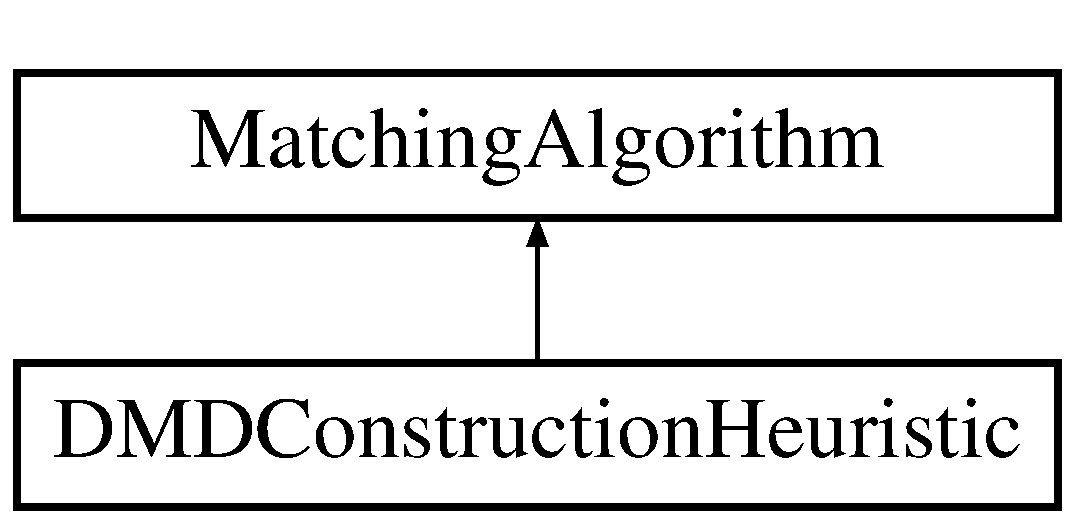
\includegraphics[height=2.000000cm]{classDMDConstructionHeuristic}
\end{center}
\end{figure}
\subsection*{Public Member Functions}
\begin{DoxyCompactItemize}
\item 
\textbf{ D\+M\+D\+Construction\+Heuristic} (\textbf{ Graph} $\ast$g, \textbf{ Matching} $\ast$m, float goal=100.\+0)
\item 
virtual \textbf{ $\sim$\+D\+M\+D\+Construction\+Heuristic} (void)
\item 
const char $\ast$ \textbf{ get\+Name} (void) const
\item 
void \textbf{ run} (void)
\end{DoxyCompactItemize}
\subsection*{Private Member Functions}
\begin{DoxyCompactItemize}
\item 
\textbf{ Vertex\+Label} \textbf{ find\+Min\+Deg\+Index} (const std\+::vector$<$ \textbf{ Vertex} $\ast$$>$ \&vertices)
\end{DoxyCompactItemize}
\subsection*{Private Attributes}
\begin{DoxyCompactItemize}
\item 
std\+::vector$<$ \textbf{ Vertex} $\ast$ $>$ \textbf{ Available\+Vertices}
\end{DoxyCompactItemize}
\subsection*{Static Private Attributes}
\begin{DoxyCompactItemize}
\item 
static const \textbf{ Vertex\+Label} \textbf{ Min\+Deg\+Not\+Found} = \textbf{ V\+E\+R\+T\+E\+X\+L\+A\+B\+E\+L\+\_\+\+M\+AX}
\end{DoxyCompactItemize}
\subsection*{Additional Inherited Members}


\subsection{Constructor \& Destructor Documentation}
\mbox{\label{classDMDConstructionHeuristic_a578457ff7ff24b7d3e39d4a2bd08e911}} 
\index{D\+M\+D\+Construction\+Heuristic@{D\+M\+D\+Construction\+Heuristic}!D\+M\+D\+Construction\+Heuristic@{D\+M\+D\+Construction\+Heuristic}}
\index{D\+M\+D\+Construction\+Heuristic@{D\+M\+D\+Construction\+Heuristic}!D\+M\+D\+Construction\+Heuristic@{D\+M\+D\+Construction\+Heuristic}}
\subsubsection{D\+M\+D\+Construction\+Heuristic()}
{\footnotesize\ttfamily D\+M\+D\+Construction\+Heuristic\+::\+D\+M\+D\+Construction\+Heuristic (\begin{DoxyParamCaption}\item[{\textbf{ Graph} $\ast$}]{g,  }\item[{\textbf{ Matching} $\ast$}]{m,  }\item[{float}]{goal = {\ttfamily 100.0} }\end{DoxyParamCaption})}

\mbox{\label{classDMDConstructionHeuristic_ad911ae35815f058a0b8b61733d13a765}} 
\index{D\+M\+D\+Construction\+Heuristic@{D\+M\+D\+Construction\+Heuristic}!````~D\+M\+D\+Construction\+Heuristic@{$\sim$\+D\+M\+D\+Construction\+Heuristic}}
\index{````~D\+M\+D\+Construction\+Heuristic@{$\sim$\+D\+M\+D\+Construction\+Heuristic}!D\+M\+D\+Construction\+Heuristic@{D\+M\+D\+Construction\+Heuristic}}
\subsubsection{$\sim$\+D\+M\+D\+Construction\+Heuristic()}
{\footnotesize\ttfamily virtual D\+M\+D\+Construction\+Heuristic\+::$\sim$\+D\+M\+D\+Construction\+Heuristic (\begin{DoxyParamCaption}\item[{void}]{ }\end{DoxyParamCaption})\hspace{0.3cm}{\ttfamily [inline]}, {\ttfamily [virtual]}}



\subsection{Member Function Documentation}
\mbox{\label{classDMDConstructionHeuristic_a1fdc61f310d1c1c498b73b8e1dc465d2}} 
\index{D\+M\+D\+Construction\+Heuristic@{D\+M\+D\+Construction\+Heuristic}!find\+Min\+Deg\+Index@{find\+Min\+Deg\+Index}}
\index{find\+Min\+Deg\+Index@{find\+Min\+Deg\+Index}!D\+M\+D\+Construction\+Heuristic@{D\+M\+D\+Construction\+Heuristic}}
\subsubsection{find\+Min\+Deg\+Index()}
{\footnotesize\ttfamily \textbf{ Vertex\+Label} D\+M\+D\+Construction\+Heuristic\+::find\+Min\+Deg\+Index (\begin{DoxyParamCaption}\item[{const std\+::vector$<$ \textbf{ Vertex} $\ast$$>$ \&}]{vertices }\end{DoxyParamCaption})\hspace{0.3cm}{\ttfamily [private]}}

\mbox{\label{classDMDConstructionHeuristic_a0ee1864e50b3478d6cccdd18f2502c54}} 
\index{D\+M\+D\+Construction\+Heuristic@{D\+M\+D\+Construction\+Heuristic}!get\+Name@{get\+Name}}
\index{get\+Name@{get\+Name}!D\+M\+D\+Construction\+Heuristic@{D\+M\+D\+Construction\+Heuristic}}
\subsubsection{get\+Name()}
{\footnotesize\ttfamily const char$\ast$ D\+M\+D\+Construction\+Heuristic\+::get\+Name (\begin{DoxyParamCaption}\item[{void}]{ }\end{DoxyParamCaption}) const\hspace{0.3cm}{\ttfamily [inline]}, {\ttfamily [virtual]}}



Implements \textbf{ Matching\+Algorithm} \doxyref{}{p.}{classMatchingAlgorithm_a7305edae5d74e91987bcf983b2a1171a}.

\mbox{\label{classDMDConstructionHeuristic_a49dd3ba3c89b0993922918379d3d3240}} 
\index{D\+M\+D\+Construction\+Heuristic@{D\+M\+D\+Construction\+Heuristic}!run@{run}}
\index{run@{run}!D\+M\+D\+Construction\+Heuristic@{D\+M\+D\+Construction\+Heuristic}}
\subsubsection{run()}
{\footnotesize\ttfamily void D\+M\+D\+Construction\+Heuristic\+::run (\begin{DoxyParamCaption}\item[{void}]{ }\end{DoxyParamCaption})\hspace{0.3cm}{\ttfamily [virtual]}}



Implements \textbf{ Matching\+Algorithm} \doxyref{}{p.}{classMatchingAlgorithm_aeea6c808daf03fd788c9a9feea885c41}.



\subsection{Member Data Documentation}
\mbox{\label{classDMDConstructionHeuristic_ab0bee2f81d495adf006e8859c8da6daa}} 
\index{D\+M\+D\+Construction\+Heuristic@{D\+M\+D\+Construction\+Heuristic}!Available\+Vertices@{Available\+Vertices}}
\index{Available\+Vertices@{Available\+Vertices}!D\+M\+D\+Construction\+Heuristic@{D\+M\+D\+Construction\+Heuristic}}
\subsubsection{Available\+Vertices}
{\footnotesize\ttfamily std\+::vector$<$\textbf{ Vertex}$\ast$$>$ D\+M\+D\+Construction\+Heuristic\+::\+Available\+Vertices\hspace{0.3cm}{\ttfamily [private]}}

\mbox{\label{classDMDConstructionHeuristic_a334ec36b8c295dfb0aeacc511d78202f}} 
\index{D\+M\+D\+Construction\+Heuristic@{D\+M\+D\+Construction\+Heuristic}!Min\+Deg\+Not\+Found@{Min\+Deg\+Not\+Found}}
\index{Min\+Deg\+Not\+Found@{Min\+Deg\+Not\+Found}!D\+M\+D\+Construction\+Heuristic@{D\+M\+D\+Construction\+Heuristic}}
\subsubsection{Min\+Deg\+Not\+Found}
{\footnotesize\ttfamily const \textbf{ Vertex\+Label} D\+M\+D\+Construction\+Heuristic\+::\+Min\+Deg\+Not\+Found = \textbf{ V\+E\+R\+T\+E\+X\+L\+A\+B\+E\+L\+\_\+\+M\+AX}\hspace{0.3cm}{\ttfamily [static]}, {\ttfamily [private]}}



The documentation for this class was generated from the following files\+:\begin{DoxyCompactItemize}
\item 
\textbf{ D\+M\+D\+Construction\+Heuristic.\+h}\item 
\textbf{ D\+M\+D\+Construction\+Heuristic.\+cc}\end{DoxyCompactItemize}

\section{Dummy\+File Class Reference}
\label{classDummyFile}\index{Dummy\+File@{Dummy\+File}}


a dummy \doxyref{Cvr\+Stg\+File}{p.}{classCvrStgFile} implementation to facilitate testing and debugging  




{\ttfamily \#include $<$Dummy\+File.\+h$>$}

Inheritance diagram for Dummy\+File\+:\begin{figure}[H]
\begin{center}
\leavevmode
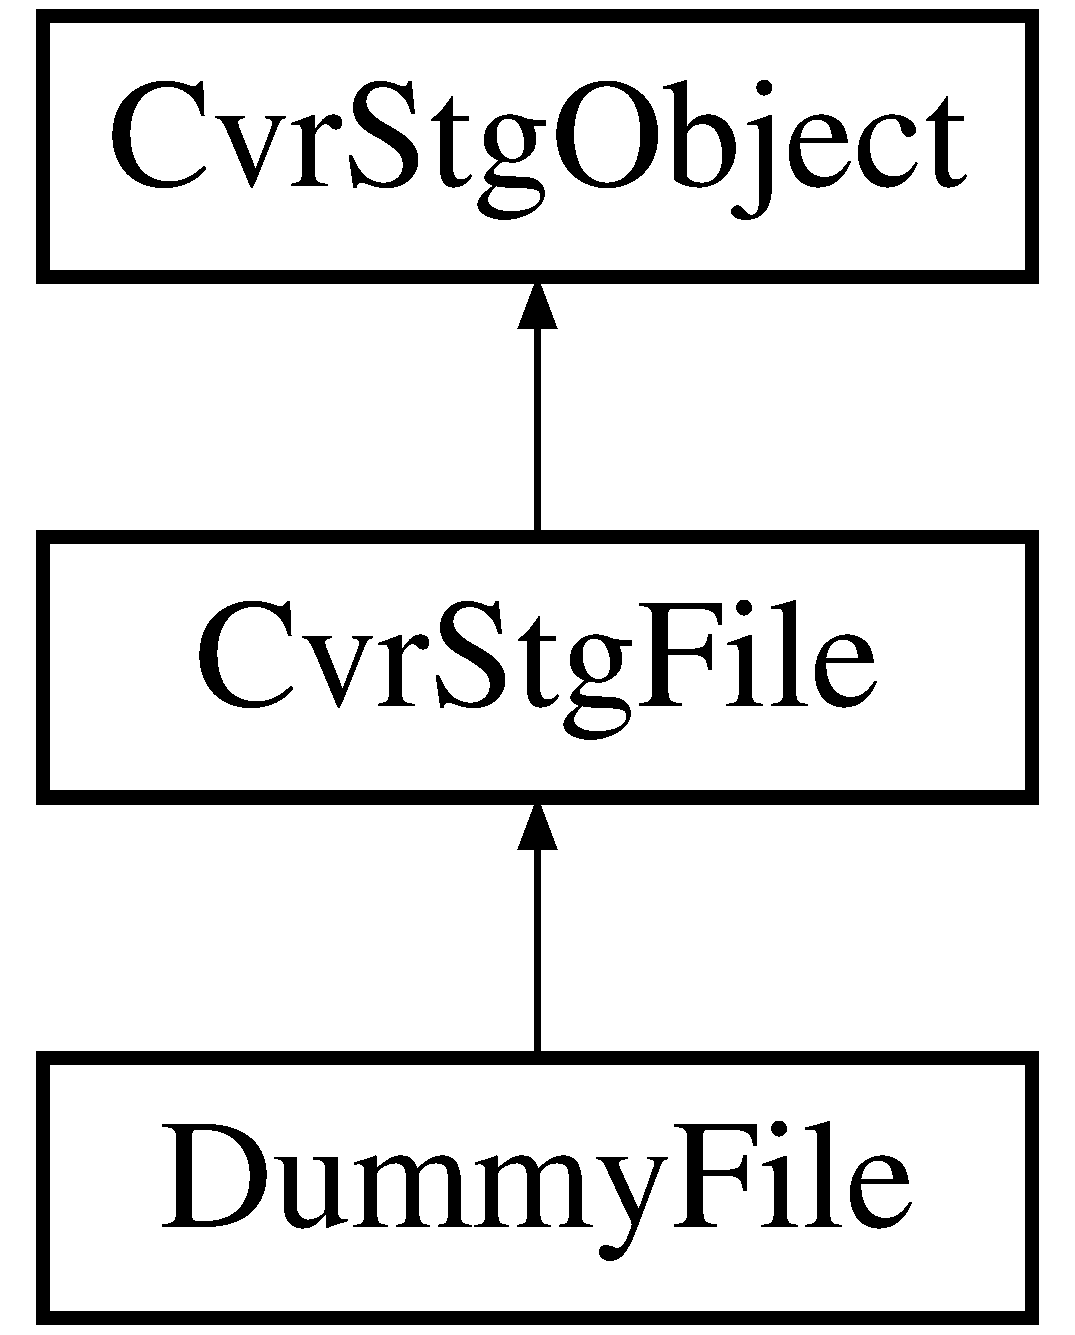
\includegraphics[height=3.000000cm]{classDummyFile}
\end{center}
\end{figure}
\subsection*{Public Member Functions}
\begin{DoxyCompactItemize}
\item 
\textbf{ Dummy\+File} (\textbf{ U\+W\+O\+R\+D16} s, std\+::vector$<$ std\+::vector$<$ bool $>$ $>$ $\ast$svam)
\item 
std\+::list$<$ \textbf{ Cvr\+Stg\+File\+::\+Property} $>$ \textbf{ get\+Properties} (void) const
\item 
unsigned long \textbf{ get\+Num\+Samples} (void) const
\item 
void \textbf{ replace\+Sample} (const \textbf{ Sample\+Pos} pos, const \textbf{ Sample\+Value} $\ast$s)
\item 
\textbf{ Sample\+Value} $\ast$ \textbf{ get\+Sample\+Value} (const \textbf{ Sample\+Pos} pos) const
\item 
std\+::vector$<$ std\+::vector$<$ bool $>$ $>$ $\ast$ \textbf{ get\+Sample\+Value\+Adjacency\+Matrix} () const
\end{DoxyCompactItemize}
\subsection*{Static Public Member Functions}
\begin{DoxyCompactItemize}
\item 
static void \textbf{ create\+Graph} (std\+::vector$<$ std\+::list$<$ \textbf{ U\+W\+O\+R\+D16} $>$ $>$ \&adjlist, \textbf{ Bit\+String} $\ast$$\ast$bs, \textbf{ Cvr\+Stg\+File} $\ast$$\ast$f, \textbf{ Selector} $\ast$$\ast$s)
\end{DoxyCompactItemize}
\subsection*{Private Attributes}
\begin{DoxyCompactItemize}
\item 
std\+::vector$<$ \textbf{ U\+W\+O\+R\+D16} $>$ \textbf{ Samples}
\item 
std\+::vector$<$ std\+::vector$<$ bool $>$ $>$ $\ast$ \textbf{ Sample\+Value\+Adjacency\+Matrix}
\end{DoxyCompactItemize}
\subsection*{Static Private Attributes}
\begin{DoxyCompactItemize}
\item 
static const unsigned short \textbf{ Samples\+Per\+Vertex} = 2
\item 
static const \textbf{ Emb\+Value} \textbf{ Emb\+Value\+Modulus} = 2
\end{DoxyCompactItemize}
\subsection*{Additional Inherited Members}


\subsection{Constructor \& Destructor Documentation}
\mbox{\label{classDummyFile_a94c2eff9aa3f00a5164c4089601d87f5}} 
\index{Dummy\+File@{Dummy\+File}!Dummy\+File@{Dummy\+File}}
\index{Dummy\+File@{Dummy\+File}!Dummy\+File@{Dummy\+File}}
\subsubsection{Dummy\+File()}
{\footnotesize\ttfamily Dummy\+File\+::\+Dummy\+File (\begin{DoxyParamCaption}\item[{\textbf{ U\+W\+O\+R\+D16}}]{s,  }\item[{std\+::vector$<$ std\+::vector$<$ bool $>$ $>$ $\ast$}]{svam }\end{DoxyParamCaption})}

construct a \doxyref{Dummy\+File}{p.}{classDummyFile} object containing the sample values 0,1,...,s-\/1 
\begin{DoxyParams}{Parameters}
{\em s} & the size of the \doxyref{Dummy\+File}{p.}{classDummyFile} (i.\+e. the number of samples it should contain) \\
\hline
{\em svam} & the Sample\+Value\+Adjacency\+Matrix for the Samples in this file \\
\hline
\end{DoxyParams}


\subsection{Member Function Documentation}
\mbox{\label{classDummyFile_a107e54b5336510f0e336db820248011e}} 
\index{Dummy\+File@{Dummy\+File}!create\+Graph@{create\+Graph}}
\index{create\+Graph@{create\+Graph}!Dummy\+File@{Dummy\+File}}
\subsubsection{create\+Graph()}
{\footnotesize\ttfamily void Dummy\+File\+::create\+Graph (\begin{DoxyParamCaption}\item[{std\+::vector$<$ std\+::list$<$ \textbf{ U\+W\+O\+R\+D16} $>$ $>$ \&}]{adjlist,  }\item[{\textbf{ Bit\+String} $\ast$$\ast$}]{bs,  }\item[{\textbf{ Cvr\+Stg\+File} $\ast$$\ast$}]{f,  }\item[{\textbf{ Selector} $\ast$$\ast$}]{s }\end{DoxyParamCaption})\hspace{0.3cm}{\ttfamily [static]}}

create a \doxyref{Bit\+String}{p.}{classBitString}, a \doxyref{Dummy\+File}{p.}{classDummyFile} and a \doxyref{Selector}{p.}{classSelector} that together will produce a graph like described by the adjacency list 
\begin{DoxyParams}{Parameters}
{\em adjlist} & an adjacency list describing the \char`\"{}target graph\char`\"{} \\
\hline
{\em bs} & will be filled with the \doxyref{Bit\+String}{p.}{classBitString} \\
\hline
{\em f} & will be filled with the \doxyref{Dummy\+File}{p.}{classDummyFile} \\
\hline
{\em s} & will be filled with the \doxyref{Selector}{p.}{classSelector}\\
\hline
\end{DoxyParams}
Constructing a \doxyref{Graph}{p.}{classGraph} object with \char`\"{}\+Graph ($\ast$f, $\ast$$\ast$bs, $\ast$$\ast$s)\char`\"{} will result in a graph of the form of adjlist.

The constructed graph has the following form\+: Samples\+Per\+Vertex == 2, Emb\+Value\+Modulus = 2 every vertex has a sample value with bit == 0 at index 0 and one with bit == 1 at index 1, if two vertices are adjacent, one end of the edge is at index 0 of the vertex with the lower vertex label and the other end of the edge is at index 1 of the vertex with the higher vertex label. The distance between vertex with label i and vertex with label j is \+: 2$\ast$$\vert$j -\/ i$\vert$ + 1 \mbox{\label{classDummyFile_a79290dd8bd87a2fabf01f8453d4ce9f0}} 
\index{Dummy\+File@{Dummy\+File}!get\+Num\+Samples@{get\+Num\+Samples}}
\index{get\+Num\+Samples@{get\+Num\+Samples}!Dummy\+File@{Dummy\+File}}
\subsubsection{get\+Num\+Samples()}
{\footnotesize\ttfamily unsigned long Dummy\+File\+::get\+Num\+Samples (\begin{DoxyParamCaption}\item[{void}]{ }\end{DoxyParamCaption}) const\hspace{0.3cm}{\ttfamily [virtual]}}

get the number of samples in this \doxyref{Cvr\+Stg\+Object}{p.}{classCvrStgObject} 

Implements \textbf{ Cvr\+Stg\+Object} \doxyref{}{p.}{classCvrStgObject_a80ae8f095b66683e5207adf8ff8265b4}.

\mbox{\label{classDummyFile_a40d1703beb749e1d6207b7d9eff8777f}} 
\index{Dummy\+File@{Dummy\+File}!get\+Properties@{get\+Properties}}
\index{get\+Properties@{get\+Properties}!Dummy\+File@{Dummy\+File}}
\subsubsection{get\+Properties()}
{\footnotesize\ttfamily std\+::list$<$ \textbf{ Cvr\+Stg\+File\+::\+Property} $>$ Dummy\+File\+::get\+Properties (\begin{DoxyParamCaption}\item[{void}]{ }\end{DoxyParamCaption}) const\hspace{0.3cm}{\ttfamily [virtual]}}



Implements \textbf{ Cvr\+Stg\+File} \doxyref{}{p.}{classCvrStgFile_afe2f570ea6447c0636093b44ff7793cc}.

\mbox{\label{classDummyFile_a44e79fbed4d236321e47d47a9e916e29}} 
\index{Dummy\+File@{Dummy\+File}!get\+Sample\+Value@{get\+Sample\+Value}}
\index{get\+Sample\+Value@{get\+Sample\+Value}!Dummy\+File@{Dummy\+File}}
\subsubsection{get\+Sample\+Value()}
{\footnotesize\ttfamily \textbf{ Sample\+Value} $\ast$ Dummy\+File\+::get\+Sample\+Value (\begin{DoxyParamCaption}\item[{const \textbf{ Sample\+Pos}}]{pos }\end{DoxyParamCaption}) const\hspace{0.3cm}{\ttfamily [virtual]}}

get the sample at position pos 
\begin{DoxyParams}{Parameters}
{\em pos} & the position of a sample (must be in 0...\doxyref{get\+Num\+Samples()}{p.}{classDummyFile_a79290dd8bd87a2fabf01f8453d4ce9f0}-\/1) \\
\hline
\end{DoxyParams}
\begin{DoxyReturn}{Returns}
the sample at the given position
\end{DoxyReturn}
The sample object is created in this function and should be deleted by the caller. The derived class should check the condition(s) given above in its Implementation of this function. 

Implements \textbf{ Cvr\+Stg\+Object} \doxyref{}{p.}{classCvrStgObject_ac77a8da85a4f7b53e2166e990dfaa4f2}.

\mbox{\label{classDummyFile_a29830fce407665c63b5e00dc9808f146}} 
\index{Dummy\+File@{Dummy\+File}!get\+Sample\+Value\+Adjacency\+Matrix@{get\+Sample\+Value\+Adjacency\+Matrix}}
\index{get\+Sample\+Value\+Adjacency\+Matrix@{get\+Sample\+Value\+Adjacency\+Matrix}!Dummy\+File@{Dummy\+File}}
\subsubsection{get\+Sample\+Value\+Adjacency\+Matrix()}
{\footnotesize\ttfamily std\+::vector$<$std\+::vector$<$bool$>$ $>$$\ast$ Dummy\+File\+::get\+Sample\+Value\+Adjacency\+Matrix (\begin{DoxyParamCaption}{ }\end{DoxyParamCaption}) const\hspace{0.3cm}{\ttfamily [inline]}}

\mbox{\label{classDummyFile_a702ca13d4515e719785b6c7b670354bb}} 
\index{Dummy\+File@{Dummy\+File}!replace\+Sample@{replace\+Sample}}
\index{replace\+Sample@{replace\+Sample}!Dummy\+File@{Dummy\+File}}
\subsubsection{replace\+Sample()}
{\footnotesize\ttfamily void Dummy\+File\+::replace\+Sample (\begin{DoxyParamCaption}\item[{const \textbf{ Sample\+Pos}}]{pos,  }\item[{const \textbf{ Sample\+Value} $\ast$}]{s }\end{DoxyParamCaption})\hspace{0.3cm}{\ttfamily [virtual]}}

replace a sample thus (possibly) altering the value of the bit returned by Sample\+Value-\/$>$get\+Bit() 
\begin{DoxyParams}{Parameters}
{\em pos} & the position of the sample (must be in 0...\doxyref{get\+Num\+Samples()}{p.}{classDummyFile_a79290dd8bd87a2fabf01f8453d4ce9f0}-\/1) \\
\hline
{\em s} & the sample value that should replace the current sample value (must be of correct type for this \doxyref{Cvr\+Stg\+Object}{p.}{classCvrStgObject})\\
\hline
\end{DoxyParams}
The derived class should check the condition(s) given above in its Implementation of this function. 

Implements \textbf{ Cvr\+Stg\+Object} \doxyref{}{p.}{classCvrStgObject_a3068d6a9dcc1c0b8bde2f081cfde6ce5}.



\subsection{Member Data Documentation}
\mbox{\label{classDummyFile_aa2ec37494bf0cb97569ab81a93f38b59}} 
\index{Dummy\+File@{Dummy\+File}!Emb\+Value\+Modulus@{Emb\+Value\+Modulus}}
\index{Emb\+Value\+Modulus@{Emb\+Value\+Modulus}!Dummy\+File@{Dummy\+File}}
\subsubsection{Emb\+Value\+Modulus}
{\footnotesize\ttfamily const \textbf{ Emb\+Value} Dummy\+File\+::\+Emb\+Value\+Modulus = 2\hspace{0.3cm}{\ttfamily [static]}, {\ttfamily [private]}}

\mbox{\label{classDummyFile_a709877388004e7a4fd55e330270ef610}} 
\index{Dummy\+File@{Dummy\+File}!Samples@{Samples}}
\index{Samples@{Samples}!Dummy\+File@{Dummy\+File}}
\subsubsection{Samples}
{\footnotesize\ttfamily std\+::vector$<$\textbf{ U\+W\+O\+R\+D16}$>$ Dummy\+File\+::\+Samples\hspace{0.3cm}{\ttfamily [private]}}

\mbox{\label{classDummyFile_acc0267226ad4c85d34f4e4bfa5088ef4}} 
\index{Dummy\+File@{Dummy\+File}!Samples\+Per\+Vertex@{Samples\+Per\+Vertex}}
\index{Samples\+Per\+Vertex@{Samples\+Per\+Vertex}!Dummy\+File@{Dummy\+File}}
\subsubsection{Samples\+Per\+Vertex}
{\footnotesize\ttfamily const unsigned short Dummy\+File\+::\+Samples\+Per\+Vertex = 2\hspace{0.3cm}{\ttfamily [static]}, {\ttfamily [private]}}

\mbox{\label{classDummyFile_ab061a391905b948f72f6c59688258dba}} 
\index{Dummy\+File@{Dummy\+File}!Sample\+Value\+Adjacency\+Matrix@{Sample\+Value\+Adjacency\+Matrix}}
\index{Sample\+Value\+Adjacency\+Matrix@{Sample\+Value\+Adjacency\+Matrix}!Dummy\+File@{Dummy\+File}}
\subsubsection{Sample\+Value\+Adjacency\+Matrix}
{\footnotesize\ttfamily std\+::vector$<$std\+::vector$<$bool$>$ $>$$\ast$ Dummy\+File\+::\+Sample\+Value\+Adjacency\+Matrix\hspace{0.3cm}{\ttfamily [private]}}



The documentation for this class was generated from the following files\+:\begin{DoxyCompactItemize}
\item 
\textbf{ Dummy\+File.\+h}\item 
\textbf{ Dummy\+File.\+cc}\end{DoxyCompactItemize}

\section{Dummy\+Sample\+Value Class Reference}
\label{classDummySampleValue}\index{Dummy\+Sample\+Value@{Dummy\+Sample\+Value}}


{\ttfamily \#include $<$Dummy\+Sample\+Value.\+h$>$}

Inheritance diagram for Dummy\+Sample\+Value\+:\begin{figure}[H]
\begin{center}
\leavevmode
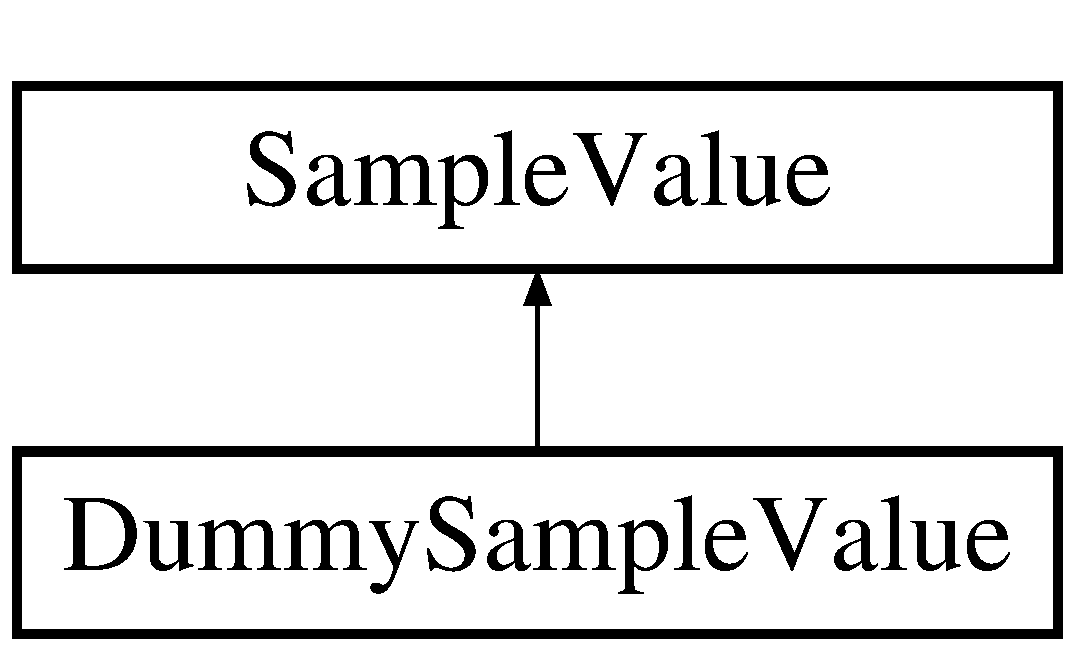
\includegraphics[height=2.000000cm]{classDummySampleValue}
\end{center}
\end{figure}
\subsection*{Public Member Functions}
\begin{DoxyCompactItemize}
\item 
\textbf{ Dummy\+Sample\+Value} (\textbf{ U\+W\+O\+R\+D16} v)
\item 
\textbf{ U\+W\+O\+R\+D16} \textbf{ get\+Value} (void) const
\item 
\textbf{ U\+W\+O\+R\+D32} \textbf{ calc\+Distance} (const \textbf{ Sample\+Value} $\ast$s) const
\item 
bool \textbf{ is\+Neighbour} (const \textbf{ Sample\+Value} $\ast$s) const
\item 
\textbf{ Sample\+Value} $\ast$ \textbf{ get\+Nearest\+Target\+Sample\+Value} (\textbf{ Emb\+Value} t) const
\item 
std\+::string \textbf{ get\+Name} (void) const
\end{DoxyCompactItemize}
\subsection*{Private Attributes}
\begin{DoxyCompactItemize}
\item 
\textbf{ U\+W\+O\+R\+D16} \textbf{ Value}
\end{DoxyCompactItemize}
\subsection*{Additional Inherited Members}


\subsection{Constructor \& Destructor Documentation}
\mbox{\label{classDummySampleValue_adcc002e8d5372432b673f40e4bf36c15}} 
\index{Dummy\+Sample\+Value@{Dummy\+Sample\+Value}!Dummy\+Sample\+Value@{Dummy\+Sample\+Value}}
\index{Dummy\+Sample\+Value@{Dummy\+Sample\+Value}!Dummy\+Sample\+Value@{Dummy\+Sample\+Value}}
\subsubsection{Dummy\+Sample\+Value()}
{\footnotesize\ttfamily Dummy\+Sample\+Value\+::\+Dummy\+Sample\+Value (\begin{DoxyParamCaption}\item[{\textbf{ U\+W\+O\+R\+D16}}]{v }\end{DoxyParamCaption})\hspace{0.3cm}{\ttfamily [inline]}}



\subsection{Member Function Documentation}
\mbox{\label{classDummySampleValue_ac3af289d7b12a404aebb4df17cfd3122}} 
\index{Dummy\+Sample\+Value@{Dummy\+Sample\+Value}!calc\+Distance@{calc\+Distance}}
\index{calc\+Distance@{calc\+Distance}!Dummy\+Sample\+Value@{Dummy\+Sample\+Value}}
\subsubsection{calc\+Distance()}
{\footnotesize\ttfamily \textbf{ U\+W\+O\+R\+D32} Dummy\+Sample\+Value\+::calc\+Distance (\begin{DoxyParamCaption}\item[{const \textbf{ Sample\+Value} $\ast$}]{s }\end{DoxyParamCaption}) const\hspace{0.3cm}{\ttfamily [virtual]}}

calculate the distance as $\vert$ Value -\/ s-\/$>$Value $\vert$ 

Implements \textbf{ Sample\+Value} \doxyref{}{p.}{classSampleValue_aa7e5d9b69203f6f6edf97c79319232dd}.

\mbox{\label{classDummySampleValue_aba495f69560f9341acda9227878975a4}} 
\index{Dummy\+Sample\+Value@{Dummy\+Sample\+Value}!get\+Name@{get\+Name}}
\index{get\+Name@{get\+Name}!Dummy\+Sample\+Value@{Dummy\+Sample\+Value}}
\subsubsection{get\+Name()}
{\footnotesize\ttfamily std\+::string Dummy\+Sample\+Value\+::get\+Name (\begin{DoxyParamCaption}\item[{void}]{ }\end{DoxyParamCaption}) const\hspace{0.3cm}{\ttfamily [virtual]}}

return a short name uniquely identifying this sample value 

Implements \textbf{ Sample\+Value} \doxyref{}{p.}{classSampleValue_aeaf5c46ec6d023840e9773604b20d25c}.

\mbox{\label{classDummySampleValue_a5920eb5fb6d87e8fbd8f6320a8a5f3f9}} 
\index{Dummy\+Sample\+Value@{Dummy\+Sample\+Value}!get\+Nearest\+Target\+Sample\+Value@{get\+Nearest\+Target\+Sample\+Value}}
\index{get\+Nearest\+Target\+Sample\+Value@{get\+Nearest\+Target\+Sample\+Value}!Dummy\+Sample\+Value@{Dummy\+Sample\+Value}}
\subsubsection{get\+Nearest\+Target\+Sample\+Value()}
{\footnotesize\ttfamily \textbf{ Sample\+Value} $\ast$ Dummy\+Sample\+Value\+::get\+Nearest\+Target\+Sample\+Value (\begin{DoxyParamCaption}\item[{\textbf{ Emb\+Value}}]{t }\end{DoxyParamCaption}) const\hspace{0.3cm}{\ttfamily [virtual]}}

get the nearest (with the least distance to this sample value) sample value whose embedded value equals the specified target 
\begin{DoxyParams}{Parameters}
{\em t} & the target embedded value\\
\hline
\end{DoxyParams}
If two or more target sample values have equal distance each of them should be returned with equal probability.

The returned \doxyref{Sample\+Value}{p.}{classSampleValue} object should be deleted by the callser. 

Implements \textbf{ Sample\+Value} \doxyref{}{p.}{classSampleValue_aeca3fc1fd34c09d2244706b010935c2c}.

\mbox{\label{classDummySampleValue_a555d0ffd2e403a99bcdf589f7ac68b44}} 
\index{Dummy\+Sample\+Value@{Dummy\+Sample\+Value}!get\+Value@{get\+Value}}
\index{get\+Value@{get\+Value}!Dummy\+Sample\+Value@{Dummy\+Sample\+Value}}
\subsubsection{get\+Value()}
{\footnotesize\ttfamily \textbf{ U\+W\+O\+R\+D16} Dummy\+Sample\+Value\+::get\+Value (\begin{DoxyParamCaption}\item[{void}]{ }\end{DoxyParamCaption}) const\hspace{0.3cm}{\ttfamily [inline]}}

\mbox{\label{classDummySampleValue_a63875aaa574e70c8f1aa881ebe60dede}} 
\index{Dummy\+Sample\+Value@{Dummy\+Sample\+Value}!is\+Neighbour@{is\+Neighbour}}
\index{is\+Neighbour@{is\+Neighbour}!Dummy\+Sample\+Value@{Dummy\+Sample\+Value}}
\subsubsection{is\+Neighbour()}
{\footnotesize\ttfamily bool Dummy\+Sample\+Value\+::is\+Neighbour (\begin{DoxyParamCaption}\item[{const \textbf{ Sample\+Value} $\ast$}]{s }\end{DoxyParamCaption}) const\hspace{0.3cm}{\ttfamily [virtual]}}

return from the contents of the Sample\+Value\+Adjacency\+Matrix in the \doxyref{Dummy\+File}{p.}{classDummyFile} 

Reimplemented from \textbf{ Sample\+Value} \doxyref{}{p.}{classSampleValue_a6f746349802439be40062a7a27d118fb}.



\subsection{Member Data Documentation}
\mbox{\label{classDummySampleValue_a9545e16ad327f0ca5282ecaf7958f83e}} 
\index{Dummy\+Sample\+Value@{Dummy\+Sample\+Value}!Value@{Value}}
\index{Value@{Value}!Dummy\+Sample\+Value@{Dummy\+Sample\+Value}}
\subsubsection{Value}
{\footnotesize\ttfamily \textbf{ U\+W\+O\+R\+D16} Dummy\+Sample\+Value\+::\+Value\hspace{0.3cm}{\ttfamily [private]}}



The documentation for this class was generated from the following files\+:\begin{DoxyCompactItemize}
\item 
\textbf{ Dummy\+Sample\+Value.\+h}\item 
\textbf{ Dummy\+Sample\+Value.\+cc}\end{DoxyCompactItemize}

\section{Edge Class Reference}
\label{classEdge}\index{Edge@{Edge}}


{\ttfamily \#include $<$Edge.\+h$>$}

\subsection*{Public Member Functions}
\begin{DoxyCompactItemize}
\item 
\textbf{ Edge} (void)
\item 
\textbf{ Edge} (\textbf{ Vertex} $\ast$v1, unsigned short idx1, \textbf{ Vertex} $\ast$v2, unsigned short idx2)
\item 
\textbf{ Edge} (const \textbf{ Edge} \&e)
\item 
\textbf{ Vertex} $\ast$ \textbf{ get\+Vertex1} (void) const
\item 
void \textbf{ set\+Vertex1} (\textbf{ Vertex} $\ast$v)
\item 
\textbf{ Vertex} $\ast$ \textbf{ get\+Vertex2} (void) const
\item 
unsigned short \textbf{ get\+Index1} (void) const
\item 
void \textbf{ set\+Index1} (unsigned short i)
\item 
unsigned short \textbf{ get\+Index2} (void) const
\item 
\textbf{ U\+W\+O\+R\+D32} \textbf{ get\+Weight} (void)
\item 
void \textbf{ set} (\textbf{ Vertex} $\ast$v1, unsigned short idx1, \textbf{ Vertex} $\ast$v2, unsigned short idx2)
\item 
void \textbf{ set1} (\textbf{ Vertex} $\ast$v1, unsigned short idx1)
\item 
void \textbf{ set2} (\textbf{ Vertex} $\ast$v2, unsigned short idx2)
\item 
bool \textbf{ operator==} (const \textbf{ Edge} \&e) const
\item 
bool \textbf{ operator!=} (const \textbf{ Edge} \&e) const
\item 
void \textbf{ swap} (void)
\item 
bool \textbf{ contains} (const \textbf{ Vertex} $\ast$v) const
\item 
\textbf{ Vertex} $\ast$ \textbf{ get\+Other\+Vertex} (const \textbf{ Vertex} $\ast$v) const
\item 
\textbf{ Sample\+Pos} \textbf{ get\+Sample\+Pos} (\textbf{ Vertex} $\ast$v) const
\item 
\textbf{ Sample\+Value} $\ast$ \textbf{ get\+Original\+Sample\+Value} (\textbf{ Vertex} $\ast$v) const
\item 
\textbf{ Sample\+Value} $\ast$ \textbf{ get\+Replacing\+Sample\+Value} (\textbf{ Vertex} $\ast$v) const
\item 
void \textbf{ print} (unsigned short spc=0) const
\end{DoxyCompactItemize}
\subsection*{Private Attributes}
\begin{DoxyCompactItemize}
\item 
\textbf{ Vertex} $\ast$ \textbf{ Vertex1}
\item 
unsigned short \textbf{ Index1}
\begin{DoxyCompactList}\small\item\em contains the index of the sample (of those in Vertex1) that will be changed (if this edge is used) \end{DoxyCompactList}\item 
\textbf{ Vertex} $\ast$ \textbf{ Vertex2}
\item 
unsigned short \textbf{ Index2}
\begin{DoxyCompactList}\small\item\em contains the index of the sample (of those in Vertex2) that will be changed (if this edge is used) \end{DoxyCompactList}\item 
\textbf{ U\+W\+O\+R\+D32} \textbf{ Weight}
\end{DoxyCompactItemize}


\subsection{Constructor \& Destructor Documentation}
\mbox{\label{classEdge_a45da6ae146df7547a4c7a86603e7a570}} 
\index{Edge@{Edge}!Edge@{Edge}}
\index{Edge@{Edge}!Edge@{Edge}}
\subsubsection{Edge()\hspace{0.1cm}{\footnotesize\ttfamily [1/3]}}
{\footnotesize\ttfamily Edge\+::\+Edge (\begin{DoxyParamCaption}\item[{void}]{ }\end{DoxyParamCaption})\hspace{0.3cm}{\ttfamily [inline]}}

default constructor -\/ does not create a useful object \mbox{\label{classEdge_a646d0b1057d6961de70dee774bdef3a4}} 
\index{Edge@{Edge}!Edge@{Edge}}
\index{Edge@{Edge}!Edge@{Edge}}
\subsubsection{Edge()\hspace{0.1cm}{\footnotesize\ttfamily [2/3]}}
{\footnotesize\ttfamily Edge\+::\+Edge (\begin{DoxyParamCaption}\item[{\textbf{ Vertex} $\ast$}]{v1,  }\item[{unsigned short}]{idx1,  }\item[{\textbf{ Vertex} $\ast$}]{v2,  }\item[{unsigned short}]{idx2 }\end{DoxyParamCaption})}

constructs an edge object \mbox{\label{classEdge_a70ed9f4d5f93c9cc5273a34361781532}} 
\index{Edge@{Edge}!Edge@{Edge}}
\index{Edge@{Edge}!Edge@{Edge}}
\subsubsection{Edge()\hspace{0.1cm}{\footnotesize\ttfamily [3/3]}}
{\footnotesize\ttfamily Edge\+::\+Edge (\begin{DoxyParamCaption}\item[{const \textbf{ Edge} \&}]{e }\end{DoxyParamCaption})}

copy constructor 

\subsection{Member Function Documentation}
\mbox{\label{classEdge_a382681c66e048bb4bdfbd226db6958de}} 
\index{Edge@{Edge}!contains@{contains}}
\index{contains@{contains}!Edge@{Edge}}
\subsubsection{contains()}
{\footnotesize\ttfamily bool Edge\+::contains (\begin{DoxyParamCaption}\item[{const \textbf{ Vertex} $\ast$}]{v }\end{DoxyParamCaption}) const}

\begin{DoxyReturn}{Returns}
true iff this edge contains the vertex v 
\end{DoxyReturn}
\mbox{\label{classEdge_a10939171ecd22a7839f6986dae97279f}} 
\index{Edge@{Edge}!get\+Index1@{get\+Index1}}
\index{get\+Index1@{get\+Index1}!Edge@{Edge}}
\subsubsection{get\+Index1()}
{\footnotesize\ttfamily unsigned short Edge\+::get\+Index1 (\begin{DoxyParamCaption}\item[{void}]{ }\end{DoxyParamCaption}) const\hspace{0.3cm}{\ttfamily [inline]}}

\mbox{\label{classEdge_a2c9cbfe1125d3ca19e36bceed5612dbe}} 
\index{Edge@{Edge}!get\+Index2@{get\+Index2}}
\index{get\+Index2@{get\+Index2}!Edge@{Edge}}
\subsubsection{get\+Index2()}
{\footnotesize\ttfamily unsigned short Edge\+::get\+Index2 (\begin{DoxyParamCaption}\item[{void}]{ }\end{DoxyParamCaption}) const\hspace{0.3cm}{\ttfamily [inline]}}

\mbox{\label{classEdge_ac68dfbcc1e393685e9de05237215ae0c}} 
\index{Edge@{Edge}!get\+Original\+Sample\+Value@{get\+Original\+Sample\+Value}}
\index{get\+Original\+Sample\+Value@{get\+Original\+Sample\+Value}!Edge@{Edge}}
\subsubsection{get\+Original\+Sample\+Value()}
{\footnotesize\ttfamily \textbf{ Sample\+Value} $\ast$ Edge\+::get\+Original\+Sample\+Value (\begin{DoxyParamCaption}\item[{\textbf{ Vertex} $\ast$}]{v }\end{DoxyParamCaption}) const}

get the old sample value that will be replaced to embed the bit represented by the vertex v \mbox{\label{classEdge_a58ed07f0227bcd3cc96782f953c94c0b}} 
\index{Edge@{Edge}!get\+Other\+Vertex@{get\+Other\+Vertex}}
\index{get\+Other\+Vertex@{get\+Other\+Vertex}!Edge@{Edge}}
\subsubsection{get\+Other\+Vertex()}
{\footnotesize\ttfamily \textbf{ Vertex} $\ast$ Edge\+::get\+Other\+Vertex (\begin{DoxyParamCaption}\item[{const \textbf{ Vertex} $\ast$}]{v }\end{DoxyParamCaption}) const}

get the vertex on this edge that is not equal to v \mbox{\label{classEdge_a63017c10332e6c064134bbab26a27011}} 
\index{Edge@{Edge}!get\+Replacing\+Sample\+Value@{get\+Replacing\+Sample\+Value}}
\index{get\+Replacing\+Sample\+Value@{get\+Replacing\+Sample\+Value}!Edge@{Edge}}
\subsubsection{get\+Replacing\+Sample\+Value()}
{\footnotesize\ttfamily \textbf{ Sample\+Value} $\ast$ Edge\+::get\+Replacing\+Sample\+Value (\begin{DoxyParamCaption}\item[{\textbf{ Vertex} $\ast$}]{v }\end{DoxyParamCaption}) const}

get the sample value that should replace the previous sample value to embed the bit represented by the vertex v \mbox{\label{classEdge_ae8ada19820ea7633f6b3f5cfad67bff8}} 
\index{Edge@{Edge}!get\+Sample\+Pos@{get\+Sample\+Pos}}
\index{get\+Sample\+Pos@{get\+Sample\+Pos}!Edge@{Edge}}
\subsubsection{get\+Sample\+Pos()}
{\footnotesize\ttfamily \textbf{ Sample\+Pos} Edge\+::get\+Sample\+Pos (\begin{DoxyParamCaption}\item[{\textbf{ Vertex} $\ast$}]{v }\end{DoxyParamCaption}) const}

get the position of the sample that should be changed to embed the bit represented by the vertex v \mbox{\label{classEdge_a3f5a5ae4404a59f4346f48b497c682ae}} 
\index{Edge@{Edge}!get\+Vertex1@{get\+Vertex1}}
\index{get\+Vertex1@{get\+Vertex1}!Edge@{Edge}}
\subsubsection{get\+Vertex1()}
{\footnotesize\ttfamily \textbf{ Vertex}$\ast$ Edge\+::get\+Vertex1 (\begin{DoxyParamCaption}\item[{void}]{ }\end{DoxyParamCaption}) const\hspace{0.3cm}{\ttfamily [inline]}}

\mbox{\label{classEdge_a60a4db1ce179dc036d8398672c9cde90}} 
\index{Edge@{Edge}!get\+Vertex2@{get\+Vertex2}}
\index{get\+Vertex2@{get\+Vertex2}!Edge@{Edge}}
\subsubsection{get\+Vertex2()}
{\footnotesize\ttfamily \textbf{ Vertex}$\ast$ Edge\+::get\+Vertex2 (\begin{DoxyParamCaption}\item[{void}]{ }\end{DoxyParamCaption}) const\hspace{0.3cm}{\ttfamily [inline]}}

\mbox{\label{classEdge_ac2da75a813dcd04c2af4da2180418d12}} 
\index{Edge@{Edge}!get\+Weight@{get\+Weight}}
\index{get\+Weight@{get\+Weight}!Edge@{Edge}}
\subsubsection{get\+Weight()}
{\footnotesize\ttfamily \textbf{ U\+W\+O\+R\+D32} Edge\+::get\+Weight (\begin{DoxyParamCaption}\item[{void}]{ }\end{DoxyParamCaption})}

\mbox{\label{classEdge_aad68f2cc1043548996c7ce6f4989a93d}} 
\index{Edge@{Edge}!operator"!=@{operator"!=}}
\index{operator"!=@{operator"!=}!Edge@{Edge}}
\subsubsection{operator"!=()}
{\footnotesize\ttfamily bool Edge\+::operator!= (\begin{DoxyParamCaption}\item[{const \textbf{ Edge} \&}]{e }\end{DoxyParamCaption}) const}

\mbox{\label{classEdge_a38c76499b14c3ada34f0b485f6e2a5bb}} 
\index{Edge@{Edge}!operator==@{operator==}}
\index{operator==@{operator==}!Edge@{Edge}}
\subsubsection{operator==()}
{\footnotesize\ttfamily bool Edge\+::operator== (\begin{DoxyParamCaption}\item[{const \textbf{ Edge} \&}]{e }\end{DoxyParamCaption}) const}

\mbox{\label{classEdge_a49933dc1fe12ca796ae077ea56d39cfb}} 
\index{Edge@{Edge}!print@{print}}
\index{print@{print}!Edge@{Edge}}
\subsubsection{print()}
{\footnotesize\ttfamily void Edge\+::print (\begin{DoxyParamCaption}\item[{unsigned short}]{spc = {\ttfamily 0} }\end{DoxyParamCaption}) const}

\mbox{\label{classEdge_ad0bc2e13a488d397b66d7bd674672a8e}} 
\index{Edge@{Edge}!set@{set}}
\index{set@{set}!Edge@{Edge}}
\subsubsection{set()}
{\footnotesize\ttfamily void Edge\+::set (\begin{DoxyParamCaption}\item[{\textbf{ Vertex} $\ast$}]{v1,  }\item[{unsigned short}]{idx1,  }\item[{\textbf{ Vertex} $\ast$}]{v2,  }\item[{unsigned short}]{idx2 }\end{DoxyParamCaption})}

\mbox{\label{classEdge_a058438cf83e35b0ea6322ff8e5e3eefb}} 
\index{Edge@{Edge}!set1@{set1}}
\index{set1@{set1}!Edge@{Edge}}
\subsubsection{set1()}
{\footnotesize\ttfamily void Edge\+::set1 (\begin{DoxyParamCaption}\item[{\textbf{ Vertex} $\ast$}]{v1,  }\item[{unsigned short}]{idx1 }\end{DoxyParamCaption})}

\mbox{\label{classEdge_a08854a9139fead445d8a6ddb34dfa172}} 
\index{Edge@{Edge}!set2@{set2}}
\index{set2@{set2}!Edge@{Edge}}
\subsubsection{set2()}
{\footnotesize\ttfamily void Edge\+::set2 (\begin{DoxyParamCaption}\item[{\textbf{ Vertex} $\ast$}]{v2,  }\item[{unsigned short}]{idx2 }\end{DoxyParamCaption})}

\mbox{\label{classEdge_a50d59e065b66696d25ae54427a40ea1e}} 
\index{Edge@{Edge}!set\+Index1@{set\+Index1}}
\index{set\+Index1@{set\+Index1}!Edge@{Edge}}
\subsubsection{set\+Index1()}
{\footnotesize\ttfamily void Edge\+::set\+Index1 (\begin{DoxyParamCaption}\item[{unsigned short}]{i }\end{DoxyParamCaption})\hspace{0.3cm}{\ttfamily [inline]}}

\mbox{\label{classEdge_a92c7a9a5a34934d0a9618a64db6ff0d3}} 
\index{Edge@{Edge}!set\+Vertex1@{set\+Vertex1}}
\index{set\+Vertex1@{set\+Vertex1}!Edge@{Edge}}
\subsubsection{set\+Vertex1()}
{\footnotesize\ttfamily void Edge\+::set\+Vertex1 (\begin{DoxyParamCaption}\item[{\textbf{ Vertex} $\ast$}]{v }\end{DoxyParamCaption})\hspace{0.3cm}{\ttfamily [inline]}}

\mbox{\label{classEdge_add513e10480eb84ae2398033e716e9df}} 
\index{Edge@{Edge}!swap@{swap}}
\index{swap@{swap}!Edge@{Edge}}
\subsubsection{swap()}
{\footnotesize\ttfamily void Edge\+::swap (\begin{DoxyParamCaption}\item[{void}]{ }\end{DoxyParamCaption})}

swap vertices 1 and 2 in this edge (weight is not altered) 

\subsection{Member Data Documentation}
\mbox{\label{classEdge_ab6f50ba5af2cff33b4be0af543289c70}} 
\index{Edge@{Edge}!Index1@{Index1}}
\index{Index1@{Index1}!Edge@{Edge}}
\subsubsection{Index1}
{\footnotesize\ttfamily unsigned short Edge\+::\+Index1\hspace{0.3cm}{\ttfamily [private]}}

\mbox{\label{classEdge_a7622b443cd056a4bcb4daec77aa418f2}} 
\index{Edge@{Edge}!Index2@{Index2}}
\index{Index2@{Index2}!Edge@{Edge}}
\subsubsection{Index2}
{\footnotesize\ttfamily unsigned short Edge\+::\+Index2\hspace{0.3cm}{\ttfamily [private]}}

\mbox{\label{classEdge_a1aae91fda044302e3a198d04db545477}} 
\index{Edge@{Edge}!Vertex1@{Vertex1}}
\index{Vertex1@{Vertex1}!Edge@{Edge}}
\subsubsection{Vertex1}
{\footnotesize\ttfamily \textbf{ Vertex}$\ast$ Edge\+::\+Vertex1\hspace{0.3cm}{\ttfamily [private]}}

\mbox{\label{classEdge_a64ab838b08888b8c9305fb9a57f0291d}} 
\index{Edge@{Edge}!Vertex2@{Vertex2}}
\index{Vertex2@{Vertex2}!Edge@{Edge}}
\subsubsection{Vertex2}
{\footnotesize\ttfamily \textbf{ Vertex}$\ast$ Edge\+::\+Vertex2\hspace{0.3cm}{\ttfamily [private]}}

\mbox{\label{classEdge_a9aa7a0c6a76f8b360f96ab564603b9c5}} 
\index{Edge@{Edge}!Weight@{Weight}}
\index{Weight@{Weight}!Edge@{Edge}}
\subsubsection{Weight}
{\footnotesize\ttfamily \textbf{ U\+W\+O\+R\+D32} Edge\+::\+Weight\hspace{0.3cm}{\ttfamily [private]}}



The documentation for this class was generated from the following files\+:\begin{DoxyCompactItemize}
\item 
\textbf{ Edge.\+h}\item 
\textbf{ Edge.\+cc}\end{DoxyCompactItemize}

\section{Edge\+Iterator Class Reference}
\label{classEdgeIterator}\index{Edge\+Iterator@{Edge\+Iterator}}


allows an iteration trough all edges of a vertex  




{\ttfamily \#include $<$Edge\+Iterator.\+h$>$}

\subsection*{Public Types}
\begin{DoxyCompactItemize}
\item 
enum \textbf{ I\+T\+E\+R\+A\+T\+I\+O\+N\+M\+O\+DE} \{ \textbf{ S\+A\+M\+P\+L\+E\+O\+C\+C\+U\+R\+E\+N\+CE}, 
\textbf{ S\+A\+M\+P\+L\+E\+V\+A\+L\+UE}
 \}
\end{DoxyCompactItemize}
\subsection*{Public Member Functions}
\begin{DoxyCompactItemize}
\item 
\textbf{ Edge\+Iterator} (void)
\item 
\textbf{ Edge\+Iterator} (\textbf{ Vertex} $\ast$v, \textbf{ I\+T\+E\+R\+A\+T\+I\+O\+N\+M\+O\+DE} m=\textbf{ S\+A\+M\+P\+L\+E\+O\+C\+C\+U\+R\+E\+N\+CE})
\item 
\textbf{ Edge\+Iterator} (const \textbf{ Edge\+Iterator} \&eit)
\item 
\textbf{ $\sim$\+Edge\+Iterator} (void)
\item 
const \textbf{ Edge} $\ast$ \textbf{ operator$\ast$} (void) const
\item 
void \textbf{ operator++} (void)
\item 
void \textbf{ reset} (\textbf{ Vertex} $\ast$v, \textbf{ I\+T\+E\+R\+A\+T\+I\+O\+N\+M\+O\+DE} m=\textbf{ S\+A\+M\+P\+L\+E\+O\+C\+C\+U\+R\+E\+N\+CE})
\item 
void \textbf{ reset} (\textbf{ I\+T\+E\+R\+A\+T\+I\+O\+N\+M\+O\+DE} m=\textbf{ S\+A\+M\+P\+L\+E\+O\+C\+C\+U\+R\+E\+N\+CE})
\item 
bool \textbf{ is\+Finished} (void) const
\item 
\textbf{ Vertex\+Label} \textbf{ get\+Partner\+Vertex\+Label} (void) const
\item 
void \textbf{ print} (unsigned short spc=0) const
\end{DoxyCompactItemize}
\subsection*{Static Public Member Functions}
\begin{DoxyCompactItemize}
\item 
static \textbf{ U\+W\+O\+R\+D32} \textbf{ get\+Max\+Num\+Edges} (void)
\item 
static void \textbf{ set\+Max\+Num\+Edges} (\textbf{ U\+W\+O\+R\+D32} mne)
\end{DoxyCompactItemize}
\subsection*{Private Member Functions}
\begin{DoxyCompactItemize}
\item 
void \textbf{ find\+Next\+Edge} (void)
\item 
bool \textbf{ is\+Dest\+Sample\+Value\+OK} (const \textbf{ Sample\+Value} $\ast$sv)
\end{DoxyCompactItemize}
\subsection*{Private Attributes}
\begin{DoxyCompactItemize}
\item 
\textbf{ Edge} \textbf{ Current\+Edge}
\begin{DoxyCompactList}\small\item\em the current edge (is returned by operator$\ast$) \end{DoxyCompactList}\item 
\textbf{ I\+T\+E\+R\+A\+T\+I\+O\+N\+M\+O\+DE} \textbf{ Mode}
\begin{DoxyCompactList}\small\item\em mode of iteration \end{DoxyCompactList}\item 
unsigned long $\ast$ \textbf{ S\+V\+A\+L\+Indices}
\begin{DoxyCompactList}\small\item\em contains (for every sample value) an index to the current opposite neighbour \end{DoxyCompactList}\item 
\textbf{ U\+W\+O\+R\+D32} \textbf{ Edge\+Index}
\begin{DoxyCompactList}\small\item\em the index/number of the edge that is currently returned by operator$\ast$ \end{DoxyCompactList}\item 
bool \textbf{ Finished}
\begin{DoxyCompactList}\small\item\em is true iff there are no more edges for this source vertex \end{DoxyCompactList}\item 
std\+::list$<$ \textbf{ Sample\+Occurence} $>$\+::const\+\_\+iterator \textbf{ Sample\+Occurence\+It}
\end{DoxyCompactItemize}
\subsection*{Static Private Attributes}
\begin{DoxyCompactItemize}
\item 
static \textbf{ U\+W\+O\+R\+D32} \textbf{ Max\+Num\+Edges} = \textbf{ U\+W\+O\+R\+D32\+\_\+\+M\+AX}
\begin{DoxyCompactList}\small\item\em the maximum number of edges the \doxyref{Edge\+Iterator}{p.}{classEdgeIterator} should iterate through \end{DoxyCompactList}\end{DoxyCompactItemize}


\subsection{Detailed Description}
The \doxyref{Vertex}{p.}{classVertex} that is the source for all edges is called \char`\"{}source vertex\char`\"{}. The order of the iteration through the edges is from the shortest to the longest edge. If two edges have the same length they are ordered the same way as the corresponding entries in the sample value adjacency lists (for different sample values) respectivly the destination sample occurences in the Sample\+Occurences data structure (for the same sample value).

\doxyref{Edge\+Iterator}{p.}{classEdgeIterator} uses an Sample\+Occurence\+::const\+\_\+iterator to store information about the current edge. \doxyref{Graph}{p.}{classGraph}\+:\+:(un)mark\+Deleted\+Sample\+Occurence can invalidate such iterators. It is therefore not a good idea to use Edge\+Iterators at the same time as the \doxyref{Graph}{p.}{classGraph}\+:\+:(un)mark\+Deleted\+Sample\+Occurence functionality.

{\bfseries N\+O\+TE\+:} \doxyref{Edge\+Iterator}{p.}{classEdgeIterator} relies on the \doxyref{Globals}{p.}{classGlobals} object pointed to by the Globs pointer. This means that it must be set correctly before using any method of an \doxyref{Edge\+Iterator}{p.}{classEdgeIterator} object. 

\subsection{Member Enumeration Documentation}
\mbox{\label{classEdgeIterator_a1e6b8b43d1620445bf945f667a38f06f}} 
\index{Edge\+Iterator@{Edge\+Iterator}!I\+T\+E\+R\+A\+T\+I\+O\+N\+M\+O\+DE@{I\+T\+E\+R\+A\+T\+I\+O\+N\+M\+O\+DE}}
\index{I\+T\+E\+R\+A\+T\+I\+O\+N\+M\+O\+DE@{I\+T\+E\+R\+A\+T\+I\+O\+N\+M\+O\+DE}!Edge\+Iterator@{Edge\+Iterator}}
\subsubsection{I\+T\+E\+R\+A\+T\+I\+O\+N\+M\+O\+DE}
{\footnotesize\ttfamily enum \textbf{ Edge\+Iterator\+::\+I\+T\+E\+R\+A\+T\+I\+O\+N\+M\+O\+DE}}

\begin{DoxyEnumFields}{Enumerator}
\raisebox{\heightof{T}}[0pt][0pt]{\index{S\+A\+M\+P\+L\+E\+O\+C\+C\+U\+R\+E\+N\+CE@{S\+A\+M\+P\+L\+E\+O\+C\+C\+U\+R\+E\+N\+CE}!Edge\+Iterator@{Edge\+Iterator}}\index{Edge\+Iterator@{Edge\+Iterator}!S\+A\+M\+P\+L\+E\+O\+C\+C\+U\+R\+E\+N\+CE@{S\+A\+M\+P\+L\+E\+O\+C\+C\+U\+R\+E\+N\+CE}}}\mbox{\label{classEdgeIterator_a1e6b8b43d1620445bf945f667a38f06fa6406f55724d4783ed9a29dc26ffbafc6}} 
S\+A\+M\+P\+L\+E\+O\+C\+C\+U\+R\+E\+N\+CE&\\
\hline

\raisebox{\heightof{T}}[0pt][0pt]{\index{S\+A\+M\+P\+L\+E\+V\+A\+L\+UE@{S\+A\+M\+P\+L\+E\+V\+A\+L\+UE}!Edge\+Iterator@{Edge\+Iterator}}\index{Edge\+Iterator@{Edge\+Iterator}!S\+A\+M\+P\+L\+E\+V\+A\+L\+UE@{S\+A\+M\+P\+L\+E\+V\+A\+L\+UE}}}\mbox{\label{classEdgeIterator_a1e6b8b43d1620445bf945f667a38f06fa06bb450ad4fec4b63fa6a16fa01a68d9}} 
S\+A\+M\+P\+L\+E\+V\+A\+L\+UE&\\
\hline

\end{DoxyEnumFields}


\subsection{Constructor \& Destructor Documentation}
\mbox{\label{classEdgeIterator_a7e5d6b76060848a91db6b0571bdadbb8}} 
\index{Edge\+Iterator@{Edge\+Iterator}!Edge\+Iterator@{Edge\+Iterator}}
\index{Edge\+Iterator@{Edge\+Iterator}!Edge\+Iterator@{Edge\+Iterator}}
\subsubsection{Edge\+Iterator()\hspace{0.1cm}{\footnotesize\ttfamily [1/3]}}
{\footnotesize\ttfamily Edge\+Iterator\+::\+Edge\+Iterator (\begin{DoxyParamCaption}\item[{void}]{ }\end{DoxyParamCaption})}

the default contructor -\/ does not create a valid object \mbox{\label{classEdgeIterator_ad52ffe34e5776d9ca5daebc2c8a1762d}} 
\index{Edge\+Iterator@{Edge\+Iterator}!Edge\+Iterator@{Edge\+Iterator}}
\index{Edge\+Iterator@{Edge\+Iterator}!Edge\+Iterator@{Edge\+Iterator}}
\subsubsection{Edge\+Iterator()\hspace{0.1cm}{\footnotesize\ttfamily [2/3]}}
{\footnotesize\ttfamily Edge\+Iterator\+::\+Edge\+Iterator (\begin{DoxyParamCaption}\item[{\textbf{ Vertex} $\ast$}]{v,  }\item[{\textbf{ I\+T\+E\+R\+A\+T\+I\+O\+N\+M\+O\+DE}}]{m = {\ttfamily \textbf{ S\+A\+M\+P\+L\+E\+O\+C\+C\+U\+R\+E\+N\+CE}} }\end{DoxyParamCaption})}


\begin{DoxyParams}{Parameters}
{\em v} & the source vertex \\
\hline
\end{DoxyParams}
\mbox{\label{classEdgeIterator_a8f7fdb7b330eec99bfe759e1be060dc4}} 
\index{Edge\+Iterator@{Edge\+Iterator}!Edge\+Iterator@{Edge\+Iterator}}
\index{Edge\+Iterator@{Edge\+Iterator}!Edge\+Iterator@{Edge\+Iterator}}
\subsubsection{Edge\+Iterator()\hspace{0.1cm}{\footnotesize\ttfamily [3/3]}}
{\footnotesize\ttfamily Edge\+Iterator\+::\+Edge\+Iterator (\begin{DoxyParamCaption}\item[{const \textbf{ Edge\+Iterator} \&}]{eit }\end{DoxyParamCaption})}

the copy constructor \mbox{\label{classEdgeIterator_a19c446b13783b0db2e9330b3982c4aac}} 
\index{Edge\+Iterator@{Edge\+Iterator}!````~Edge\+Iterator@{$\sim$\+Edge\+Iterator}}
\index{````~Edge\+Iterator@{$\sim$\+Edge\+Iterator}!Edge\+Iterator@{Edge\+Iterator}}
\subsubsection{$\sim$\+Edge\+Iterator()}
{\footnotesize\ttfamily Edge\+Iterator\+::$\sim$\+Edge\+Iterator (\begin{DoxyParamCaption}\item[{void}]{ }\end{DoxyParamCaption})}



\subsection{Member Function Documentation}
\mbox{\label{classEdgeIterator_ac311721ce85f5301e76edc29b0504d53}} 
\index{Edge\+Iterator@{Edge\+Iterator}!find\+Next\+Edge@{find\+Next\+Edge}}
\index{find\+Next\+Edge@{find\+Next\+Edge}!Edge\+Iterator@{Edge\+Iterator}}
\subsubsection{find\+Next\+Edge()}
{\footnotesize\ttfamily void Edge\+Iterator\+::find\+Next\+Edge (\begin{DoxyParamCaption}\item[{void}]{ }\end{DoxyParamCaption})\hspace{0.3cm}{\ttfamily [private]}}

find the shortest edge, starting the search at S\+V\+Opp\+Neighs\+Indices[0...k] set the private variables accordingly is only called to find a new destination sample value, i.\+e. if one of the S\+V\+Opp\+Neighs\+Indices[i] is changed \mbox{\label{classEdgeIterator_a60d3b8bc61a31c440cdb3566d05cb8c8}} 
\index{Edge\+Iterator@{Edge\+Iterator}!get\+Max\+Num\+Edges@{get\+Max\+Num\+Edges}}
\index{get\+Max\+Num\+Edges@{get\+Max\+Num\+Edges}!Edge\+Iterator@{Edge\+Iterator}}
\subsubsection{get\+Max\+Num\+Edges()}
{\footnotesize\ttfamily static \textbf{ U\+W\+O\+R\+D32} Edge\+Iterator\+::get\+Max\+Num\+Edges (\begin{DoxyParamCaption}\item[{void}]{ }\end{DoxyParamCaption})\hspace{0.3cm}{\ttfamily [inline]}, {\ttfamily [static]}}

\mbox{\label{classEdgeIterator_aec17c48fb9fa6f6c096fc24a8bc8b92f}} 
\index{Edge\+Iterator@{Edge\+Iterator}!get\+Partner\+Vertex\+Label@{get\+Partner\+Vertex\+Label}}
\index{get\+Partner\+Vertex\+Label@{get\+Partner\+Vertex\+Label}!Edge\+Iterator@{Edge\+Iterator}}
\subsubsection{get\+Partner\+Vertex\+Label()}
{\footnotesize\ttfamily \textbf{ Vertex\+Label} Edge\+Iterator\+::get\+Partner\+Vertex\+Label (\begin{DoxyParamCaption}\item[{void}]{ }\end{DoxyParamCaption}) const\hspace{0.3cm}{\ttfamily [inline]}}

get the label of the partner vertex \begin{DoxyReturn}{Returns}
the label of the vertex that builds the edge returned by operator$\ast$ together with Src\+Vertex 
\end{DoxyReturn}
\mbox{\label{classEdgeIterator_a5784525651bdb8d0f68171378d79a337}} 
\index{Edge\+Iterator@{Edge\+Iterator}!is\+Dest\+Sample\+Value\+OK@{is\+Dest\+Sample\+Value\+OK}}
\index{is\+Dest\+Sample\+Value\+OK@{is\+Dest\+Sample\+Value\+OK}!Edge\+Iterator@{Edge\+Iterator}}
\subsubsection{is\+Dest\+Sample\+Value\+O\+K()}
{\footnotesize\ttfamily bool Edge\+Iterator\+::is\+Dest\+Sample\+Value\+OK (\begin{DoxyParamCaption}\item[{const \textbf{ Sample\+Value} $\ast$}]{sv }\end{DoxyParamCaption})\hspace{0.3cm}{\ttfamily [private]}}

\begin{DoxyReturn}{Returns}
true iff there is a sample with value sv that is part of an edge starting at Src\+Vertex 
\end{DoxyReturn}
\mbox{\label{classEdgeIterator_a54b814ef06349cb05cec7a98530a7162}} 
\index{Edge\+Iterator@{Edge\+Iterator}!is\+Finished@{is\+Finished}}
\index{is\+Finished@{is\+Finished}!Edge\+Iterator@{Edge\+Iterator}}
\subsubsection{is\+Finished()}
{\footnotesize\ttfamily bool Edge\+Iterator\+::is\+Finished (\begin{DoxyParamCaption}\item[{void}]{ }\end{DoxyParamCaption}) const\hspace{0.3cm}{\ttfamily [inline]}}

\begin{DoxyReturn}{Returns}
true iff this \doxyref{Edge\+Iterator}{p.}{classEdgeIterator} points to the end of the list of edges of Src\+Vertex 
\end{DoxyReturn}
\mbox{\label{classEdgeIterator_abc0f5f5d8a9c4fc8514493a16f7bbb85}} 
\index{Edge\+Iterator@{Edge\+Iterator}!operator$\ast$@{operator$\ast$}}
\index{operator$\ast$@{operator$\ast$}!Edge\+Iterator@{Edge\+Iterator}}
\subsubsection{operator$\ast$()}
{\footnotesize\ttfamily const \textbf{ Edge}$\ast$ Edge\+Iterator\+::operator$\ast$ (\begin{DoxyParamCaption}\item[{void}]{ }\end{DoxyParamCaption}) const\hspace{0.3cm}{\ttfamily [inline]}}

get the current edge \begin{DoxyReturn}{Returns}
the edge that is described by the current status of this \doxyref{Edge\+Iterator}{p.}{classEdgeIterator} 
\end{DoxyReturn}
\mbox{\label{classEdgeIterator_a4ddd6595ef896f8137897745883baeaf}} 
\index{Edge\+Iterator@{Edge\+Iterator}!operator++@{operator++}}
\index{operator++@{operator++}!Edge\+Iterator@{Edge\+Iterator}}
\subsubsection{operator++()}
{\footnotesize\ttfamily void Edge\+Iterator\+::operator++ (\begin{DoxyParamCaption}\item[{void}]{ }\end{DoxyParamCaption})}

set this iterator to next edge \mbox{\label{classEdgeIterator_a47630728e64dca512adbaab0880a0394}} 
\index{Edge\+Iterator@{Edge\+Iterator}!print@{print}}
\index{print@{print}!Edge\+Iterator@{Edge\+Iterator}}
\subsubsection{print()}
{\footnotesize\ttfamily void Edge\+Iterator\+::print (\begin{DoxyParamCaption}\item[{unsigned short}]{spc = {\ttfamily 0} }\end{DoxyParamCaption}) const}

\mbox{\label{classEdgeIterator_a913b73da861648481ae7d74d927f9466}} 
\index{Edge\+Iterator@{Edge\+Iterator}!reset@{reset}}
\index{reset@{reset}!Edge\+Iterator@{Edge\+Iterator}}
\subsubsection{reset()\hspace{0.1cm}{\footnotesize\ttfamily [1/2]}}
{\footnotesize\ttfamily void Edge\+Iterator\+::reset (\begin{DoxyParamCaption}\item[{\textbf{ Vertex} $\ast$}]{v,  }\item[{\textbf{ I\+T\+E\+R\+A\+T\+I\+O\+N\+M\+O\+DE}}]{m = {\ttfamily \textbf{ S\+A\+M\+P\+L\+E\+O\+C\+C\+U\+R\+E\+N\+CE}} }\end{DoxyParamCaption})}

set this iterator to first (shortest) edge of vertex v 
\begin{DoxyParams}{Parameters}
{\em v} & new vertex (don\textquotesingle{}t change if it is N\+U\+LL) \\
\hline
\end{DoxyParams}
\mbox{\label{classEdgeIterator_a2db46e5ab5973dcc5ea40c9dcccdd225}} 
\index{Edge\+Iterator@{Edge\+Iterator}!reset@{reset}}
\index{reset@{reset}!Edge\+Iterator@{Edge\+Iterator}}
\subsubsection{reset()\hspace{0.1cm}{\footnotesize\ttfamily [2/2]}}
{\footnotesize\ttfamily void Edge\+Iterator\+::reset (\begin{DoxyParamCaption}\item[{\textbf{ I\+T\+E\+R\+A\+T\+I\+O\+N\+M\+O\+DE}}]{m = {\ttfamily \textbf{ S\+A\+M\+P\+L\+E\+O\+C\+C\+U\+R\+E\+N\+CE}} }\end{DoxyParamCaption})}

reset this iterator to first (shortest) edge \mbox{\label{classEdgeIterator_a134f9df6962195c8630db2321b3f39c4}} 
\index{Edge\+Iterator@{Edge\+Iterator}!set\+Max\+Num\+Edges@{set\+Max\+Num\+Edges}}
\index{set\+Max\+Num\+Edges@{set\+Max\+Num\+Edges}!Edge\+Iterator@{Edge\+Iterator}}
\subsubsection{set\+Max\+Num\+Edges()}
{\footnotesize\ttfamily static void Edge\+Iterator\+::set\+Max\+Num\+Edges (\begin{DoxyParamCaption}\item[{\textbf{ U\+W\+O\+R\+D32}}]{mne }\end{DoxyParamCaption})\hspace{0.3cm}{\ttfamily [inline]}, {\ttfamily [static]}}



\subsection{Member Data Documentation}
\mbox{\label{classEdgeIterator_a5bfdc881c10c2e7f1f427143fe085319}} 
\index{Edge\+Iterator@{Edge\+Iterator}!Current\+Edge@{Current\+Edge}}
\index{Current\+Edge@{Current\+Edge}!Edge\+Iterator@{Edge\+Iterator}}
\subsubsection{Current\+Edge}
{\footnotesize\ttfamily \textbf{ Edge} Edge\+Iterator\+::\+Current\+Edge\hspace{0.3cm}{\ttfamily [private]}}

\mbox{\label{classEdgeIterator_a6f8659a01c46698ae37fb4a929d2bfa7}} 
\index{Edge\+Iterator@{Edge\+Iterator}!Edge\+Index@{Edge\+Index}}
\index{Edge\+Index@{Edge\+Index}!Edge\+Iterator@{Edge\+Iterator}}
\subsubsection{Edge\+Index}
{\footnotesize\ttfamily \textbf{ U\+W\+O\+R\+D32} Edge\+Iterator\+::\+Edge\+Index\hspace{0.3cm}{\ttfamily [private]}}

\mbox{\label{classEdgeIterator_a0eb7a498646e95059198ad9c6b2e4a0a}} 
\index{Edge\+Iterator@{Edge\+Iterator}!Finished@{Finished}}
\index{Finished@{Finished}!Edge\+Iterator@{Edge\+Iterator}}
\subsubsection{Finished}
{\footnotesize\ttfamily bool Edge\+Iterator\+::\+Finished\hspace{0.3cm}{\ttfamily [private]}}

\mbox{\label{classEdgeIterator_a66f4a506bb6682d79385d89e8dcbc1d7}} 
\index{Edge\+Iterator@{Edge\+Iterator}!Max\+Num\+Edges@{Max\+Num\+Edges}}
\index{Max\+Num\+Edges@{Max\+Num\+Edges}!Edge\+Iterator@{Edge\+Iterator}}
\subsubsection{Max\+Num\+Edges}
{\footnotesize\ttfamily \textbf{ U\+W\+O\+R\+D32} Edge\+Iterator\+::\+Max\+Num\+Edges = \textbf{ U\+W\+O\+R\+D32\+\_\+\+M\+AX}\hspace{0.3cm}{\ttfamily [static]}, {\ttfamily [private]}}

\mbox{\label{classEdgeIterator_ab48d3dfdc5004cec669c9dc04c069c77}} 
\index{Edge\+Iterator@{Edge\+Iterator}!Mode@{Mode}}
\index{Mode@{Mode}!Edge\+Iterator@{Edge\+Iterator}}
\subsubsection{Mode}
{\footnotesize\ttfamily \textbf{ I\+T\+E\+R\+A\+T\+I\+O\+N\+M\+O\+DE} Edge\+Iterator\+::\+Mode\hspace{0.3cm}{\ttfamily [private]}}

\mbox{\label{classEdgeIterator_ab23539c65c464b0f88e81f402124101c}} 
\index{Edge\+Iterator@{Edge\+Iterator}!Sample\+Occurence\+It@{Sample\+Occurence\+It}}
\index{Sample\+Occurence\+It@{Sample\+Occurence\+It}!Edge\+Iterator@{Edge\+Iterator}}
\subsubsection{Sample\+Occurence\+It}
{\footnotesize\ttfamily std\+::list$<$\textbf{ Sample\+Occurence}$>$\+::const\+\_\+iterator Edge\+Iterator\+::\+Sample\+Occurence\+It\hspace{0.3cm}{\ttfamily [private]}}

contains the iterator pointing to the sample occurence that constitutes the edge together with Source\+Vertex/\+Source\+Samle\+Value\+Index \mbox{\label{classEdgeIterator_a15657a537da3adaba5977db8d2f30743}} 
\index{Edge\+Iterator@{Edge\+Iterator}!S\+V\+A\+L\+Indices@{S\+V\+A\+L\+Indices}}
\index{S\+V\+A\+L\+Indices@{S\+V\+A\+L\+Indices}!Edge\+Iterator@{Edge\+Iterator}}
\subsubsection{S\+V\+A\+L\+Indices}
{\footnotesize\ttfamily unsigned long$\ast$ Edge\+Iterator\+::\+S\+V\+A\+L\+Indices\hspace{0.3cm}{\ttfamily [private]}}



The documentation for this class was generated from the following files\+:\begin{DoxyCompactItemize}
\item 
\textbf{ Edge\+Iterator.\+h}\item 
\textbf{ Edge\+Iterator.\+cc}\end{DoxyCompactItemize}

\section{Edge\+Iterator\+Test Class Reference}
\label{classEdgeIteratorTest}\index{Edge\+Iterator\+Test@{Edge\+Iterator\+Test}}


{\ttfamily \#include $<$Edge\+Iterator\+Test.\+h$>$}

Inheritance diagram for Edge\+Iterator\+Test\+:\begin{figure}[H]
\begin{center}
\leavevmode
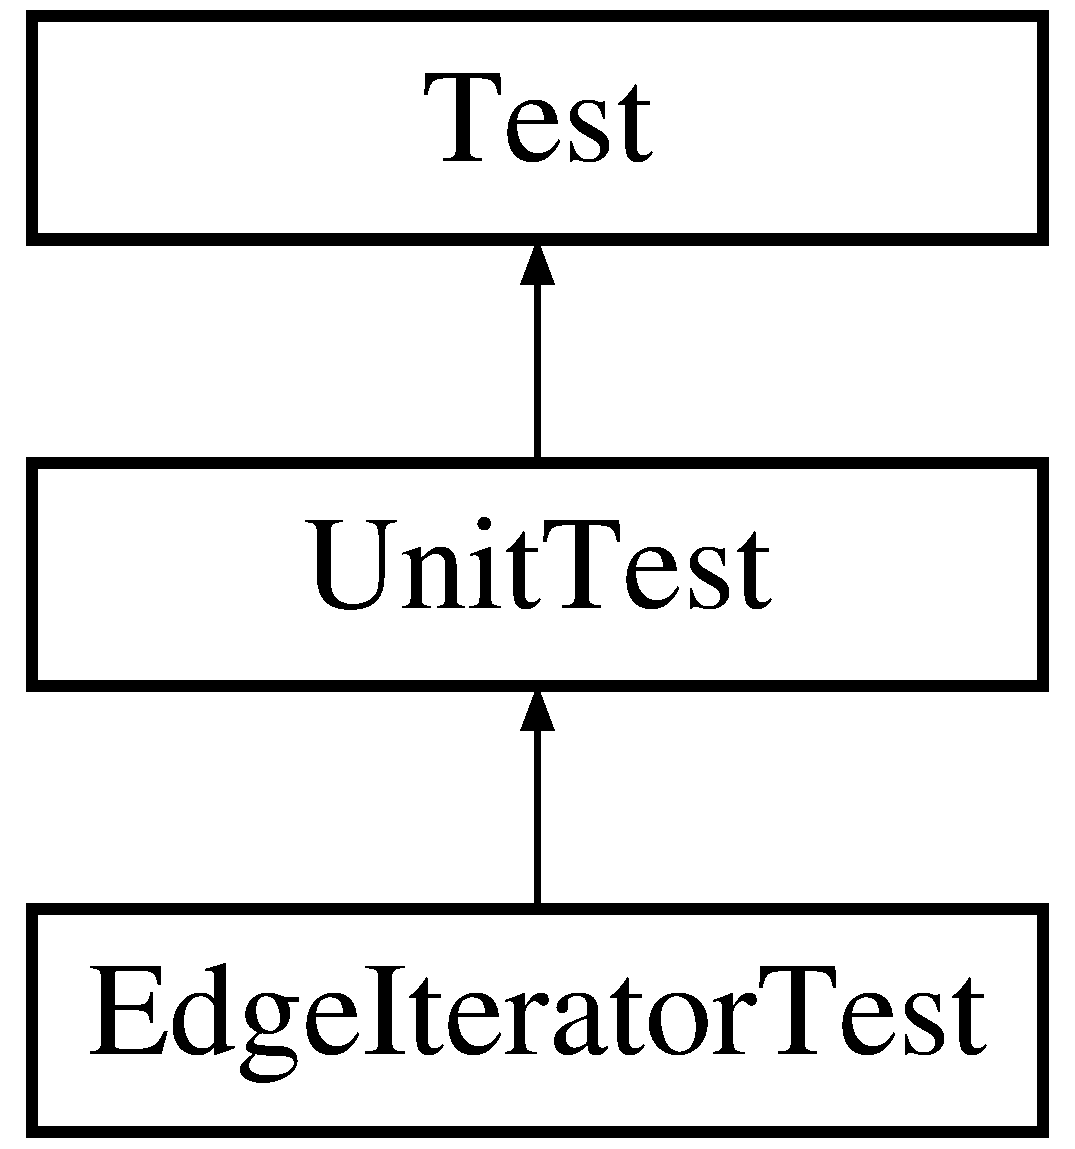
\includegraphics[height=3.000000cm]{classEdgeIteratorTest}
\end{center}
\end{figure}
\subsection*{Public Member Functions}
\begin{DoxyCompactItemize}
\item 
\textbf{ Edge\+Iterator\+Test} (\textbf{ Test\+Suite} $\ast$s)
\item 
void \textbf{ setup} (void)
\item 
void \textbf{ cleanup} (void)
\item 
void \textbf{ test\+Reference\+Iteration} (void)
\item 
void \textbf{ test\+Iteration\+Length} (void)
\end{DoxyCompactItemize}
\subsection*{Private Member Functions}
\begin{DoxyCompactItemize}
\item 
bool \textbf{ generic\+Test\+Graph\+Iteration} (\textbf{ Graph} $\ast$g, \textbf{ Edge\+Iterator\+::\+I\+T\+E\+R\+A\+T\+I\+O\+N\+M\+O\+DE} m)
\item 
bool \textbf{ generic\+Test\+Vertex\+Iteration} (\textbf{ Vertex} $\ast$srcvertex, \textbf{ Edge\+Iterator\+::\+I\+T\+E\+R\+A\+T\+I\+O\+N\+M\+O\+DE} m, const std\+::vector$<$ \textbf{ Edge} $\ast$$>$ \&edges)
\item 
bool \textbf{ generic\+Test\+Iteration\+Length} (\textbf{ Graph} $\ast$g)
\end{DoxyCompactItemize}
\subsection*{Private Attributes}
\begin{DoxyCompactItemize}
\item 
\textbf{ Bit\+String} $\ast$ \textbf{ bs1}
\item 
\textbf{ Bit\+String} $\ast$ \textbf{ bs2}
\item 
\textbf{ Cvr\+Stg\+File} $\ast$ \textbf{ f1}
\item 
\textbf{ Cvr\+Stg\+File} $\ast$ \textbf{ f2}
\item 
\textbf{ Selector} $\ast$ \textbf{ s1}
\item 
\textbf{ Selector} $\ast$ \textbf{ s2}
\item 
\textbf{ Graph} $\ast$ \textbf{ g1}
\item 
\textbf{ Graph} $\ast$ \textbf{ g2}
\item 
\textbf{ Globals} \textbf{ gl1}
\item 
\textbf{ Globals} \textbf{ gl2}
\item 
\textbf{ Bit\+String} $\ast$ \textbf{ bs10}
\item 
\textbf{ Bit\+String} $\ast$ \textbf{ bs11}
\item 
\textbf{ Bit\+String} $\ast$ \textbf{ bs12}
\item 
\textbf{ Cvr\+Stg\+File} $\ast$ \textbf{ f10}
\item 
\textbf{ Cvr\+Stg\+File} $\ast$ \textbf{ f11}
\item 
\textbf{ Cvr\+Stg\+File} $\ast$ \textbf{ f12}
\item 
\textbf{ Selector} $\ast$ \textbf{ s10}
\item 
\textbf{ Selector} $\ast$ \textbf{ s11}
\item 
\textbf{ Selector} $\ast$ \textbf{ s12}
\item 
\textbf{ Graph} $\ast$ \textbf{ g10}
\item 
\textbf{ Graph} $\ast$ \textbf{ g11}
\item 
\textbf{ Graph} $\ast$ \textbf{ g12}
\item 
\textbf{ Globals} \textbf{ gl10}
\item 
\textbf{ Globals} \textbf{ gl11}
\item 
\textbf{ Globals} \textbf{ gl12}
\end{DoxyCompactItemize}
\subsection*{Additional Inherited Members}


\subsection{Constructor \& Destructor Documentation}
\mbox{\label{classEdgeIteratorTest_a82601ecbc3b939feb92fbfb62b512dbb}} 
\index{Edge\+Iterator\+Test@{Edge\+Iterator\+Test}!Edge\+Iterator\+Test@{Edge\+Iterator\+Test}}
\index{Edge\+Iterator\+Test@{Edge\+Iterator\+Test}!Edge\+Iterator\+Test@{Edge\+Iterator\+Test}}
\subsubsection{Edge\+Iterator\+Test()}
{\footnotesize\ttfamily Edge\+Iterator\+Test\+::\+Edge\+Iterator\+Test (\begin{DoxyParamCaption}\item[{\textbf{ Test\+Suite} $\ast$}]{s }\end{DoxyParamCaption})}



\subsection{Member Function Documentation}
\mbox{\label{classEdgeIteratorTest_a7e1af6040e329046f30544cb703d2cd8}} 
\index{Edge\+Iterator\+Test@{Edge\+Iterator\+Test}!cleanup@{cleanup}}
\index{cleanup@{cleanup}!Edge\+Iterator\+Test@{Edge\+Iterator\+Test}}
\subsubsection{cleanup()}
{\footnotesize\ttfamily void Edge\+Iterator\+Test\+::cleanup (\begin{DoxyParamCaption}\item[{void}]{ }\end{DoxyParamCaption})\hspace{0.3cm}{\ttfamily [virtual]}}

cleanup the unit test -\/ called after run 

Reimplemented from \textbf{ Unit\+Test} \doxyref{}{p.}{classUnitTest_adf77efe972ee4a766d94e3f7ddc193ad}.

\mbox{\label{classEdgeIteratorTest_af6683aa7e61c472534fb36164fa71410}} 
\index{Edge\+Iterator\+Test@{Edge\+Iterator\+Test}!generic\+Test\+Graph\+Iteration@{generic\+Test\+Graph\+Iteration}}
\index{generic\+Test\+Graph\+Iteration@{generic\+Test\+Graph\+Iteration}!Edge\+Iterator\+Test@{Edge\+Iterator\+Test}}
\subsubsection{generic\+Test\+Graph\+Iteration()}
{\footnotesize\ttfamily bool Edge\+Iterator\+Test\+::generic\+Test\+Graph\+Iteration (\begin{DoxyParamCaption}\item[{\textbf{ Graph} $\ast$}]{g,  }\item[{\textbf{ Edge\+Iterator\+::\+I\+T\+E\+R\+A\+T\+I\+O\+N\+M\+O\+DE}}]{m }\end{DoxyParamCaption})\hspace{0.3cm}{\ttfamily [private]}}

\mbox{\label{classEdgeIteratorTest_a47e64a32b433e8a29190075f757c43bc}} 
\index{Edge\+Iterator\+Test@{Edge\+Iterator\+Test}!generic\+Test\+Iteration\+Length@{generic\+Test\+Iteration\+Length}}
\index{generic\+Test\+Iteration\+Length@{generic\+Test\+Iteration\+Length}!Edge\+Iterator\+Test@{Edge\+Iterator\+Test}}
\subsubsection{generic\+Test\+Iteration\+Length()}
{\footnotesize\ttfamily bool Edge\+Iterator\+Test\+::generic\+Test\+Iteration\+Length (\begin{DoxyParamCaption}\item[{\textbf{ Graph} $\ast$}]{g }\end{DoxyParamCaption})\hspace{0.3cm}{\ttfamily [private]}}

for all vertices in the graph test if get\+Degree() returns exactly the number of edges \doxyref{Edge\+Iterator}{p.}{classEdgeIterator} iterates through \mbox{\label{classEdgeIteratorTest_a01a828efc2bbe14aa50cee9a7ae2522e}} 
\index{Edge\+Iterator\+Test@{Edge\+Iterator\+Test}!generic\+Test\+Vertex\+Iteration@{generic\+Test\+Vertex\+Iteration}}
\index{generic\+Test\+Vertex\+Iteration@{generic\+Test\+Vertex\+Iteration}!Edge\+Iterator\+Test@{Edge\+Iterator\+Test}}
\subsubsection{generic\+Test\+Vertex\+Iteration()}
{\footnotesize\ttfamily bool Edge\+Iterator\+Test\+::generic\+Test\+Vertex\+Iteration (\begin{DoxyParamCaption}\item[{\textbf{ Vertex} $\ast$}]{srcvertex,  }\item[{\textbf{ Edge\+Iterator\+::\+I\+T\+E\+R\+A\+T\+I\+O\+N\+M\+O\+DE}}]{m,  }\item[{const std\+::vector$<$ \textbf{ Edge} $\ast$$>$ \&}]{edges }\end{DoxyParamCaption})\hspace{0.3cm}{\ttfamily [private]}}

check if an edge iterator for srcvertex with m iterates exactly through edges \mbox{\label{classEdgeIteratorTest_ad56dd8b150c16b3fba70d4eadb7d7bc2}} 
\index{Edge\+Iterator\+Test@{Edge\+Iterator\+Test}!setup@{setup}}
\index{setup@{setup}!Edge\+Iterator\+Test@{Edge\+Iterator\+Test}}
\subsubsection{setup()}
{\footnotesize\ttfamily void Edge\+Iterator\+Test\+::setup (\begin{DoxyParamCaption}\item[{void}]{ }\end{DoxyParamCaption})\hspace{0.3cm}{\ttfamily [virtual]}}

setup the unit test -\/ called before run

\doxyref{Unit\+Test\+::setup}{p.}{classUnitTest_ad73fdf9012b651047ea001d21f9d27ad} will (together with \doxyref{Unit\+Test\+::cleanup}{p.}{classUnitTest_adf77efe972ee4a766d94e3f7ddc193ad}) save and restore the object stored in Globs so they should be called from the corresponding functions in the derived object if the derived unit test manipulates the Globs object. 

Reimplemented from \textbf{ Unit\+Test} \doxyref{}{p.}{classUnitTest_ad73fdf9012b651047ea001d21f9d27ad}.

\mbox{\label{classEdgeIteratorTest_ac52ea6543adad6901f27e87ca63dd80a}} 
\index{Edge\+Iterator\+Test@{Edge\+Iterator\+Test}!test\+Iteration\+Length@{test\+Iteration\+Length}}
\index{test\+Iteration\+Length@{test\+Iteration\+Length}!Edge\+Iterator\+Test@{Edge\+Iterator\+Test}}
\subsubsection{test\+Iteration\+Length()}
{\footnotesize\ttfamily void Edge\+Iterator\+Test\+::test\+Iteration\+Length (\begin{DoxyParamCaption}\item[{void}]{ }\end{DoxyParamCaption})}

\mbox{\label{classEdgeIteratorTest_acbef606cf0301f1ad401cb8fb53b6fd7}} 
\index{Edge\+Iterator\+Test@{Edge\+Iterator\+Test}!test\+Reference\+Iteration@{test\+Reference\+Iteration}}
\index{test\+Reference\+Iteration@{test\+Reference\+Iteration}!Edge\+Iterator\+Test@{Edge\+Iterator\+Test}}
\subsubsection{test\+Reference\+Iteration()}
{\footnotesize\ttfamily void Edge\+Iterator\+Test\+::test\+Reference\+Iteration (\begin{DoxyParamCaption}\item[{void}]{ }\end{DoxyParamCaption})}



\subsection{Member Data Documentation}
\mbox{\label{classEdgeIteratorTest_a08d7344594c3f9b406fd5f26afbc3034}} 
\index{Edge\+Iterator\+Test@{Edge\+Iterator\+Test}!bs1@{bs1}}
\index{bs1@{bs1}!Edge\+Iterator\+Test@{Edge\+Iterator\+Test}}
\subsubsection{bs1}
{\footnotesize\ttfamily \textbf{ Bit\+String}$\ast$ Edge\+Iterator\+Test\+::bs1\hspace{0.3cm}{\ttfamily [private]}}

\mbox{\label{classEdgeIteratorTest_a240e682e43ade7e69be301cbe00fcefd}} 
\index{Edge\+Iterator\+Test@{Edge\+Iterator\+Test}!bs10@{bs10}}
\index{bs10@{bs10}!Edge\+Iterator\+Test@{Edge\+Iterator\+Test}}
\subsubsection{bs10}
{\footnotesize\ttfamily \textbf{ Bit\+String}$\ast$ Edge\+Iterator\+Test\+::bs10\hspace{0.3cm}{\ttfamily [private]}}

\mbox{\label{classEdgeIteratorTest_adaaa75fe739abcc86cfeabf8aee04285}} 
\index{Edge\+Iterator\+Test@{Edge\+Iterator\+Test}!bs11@{bs11}}
\index{bs11@{bs11}!Edge\+Iterator\+Test@{Edge\+Iterator\+Test}}
\subsubsection{bs11}
{\footnotesize\ttfamily \textbf{ Bit\+String} $\ast$ Edge\+Iterator\+Test\+::bs11\hspace{0.3cm}{\ttfamily [private]}}

\mbox{\label{classEdgeIteratorTest_adeeabfc59f8cf4f3025b30ce64c0d610}} 
\index{Edge\+Iterator\+Test@{Edge\+Iterator\+Test}!bs12@{bs12}}
\index{bs12@{bs12}!Edge\+Iterator\+Test@{Edge\+Iterator\+Test}}
\subsubsection{bs12}
{\footnotesize\ttfamily \textbf{ Bit\+String} $\ast$ Edge\+Iterator\+Test\+::bs12\hspace{0.3cm}{\ttfamily [private]}}

\mbox{\label{classEdgeIteratorTest_aa4b53f6b9f3cbcd24d17bd6bc294f1a6}} 
\index{Edge\+Iterator\+Test@{Edge\+Iterator\+Test}!bs2@{bs2}}
\index{bs2@{bs2}!Edge\+Iterator\+Test@{Edge\+Iterator\+Test}}
\subsubsection{bs2}
{\footnotesize\ttfamily \textbf{ Bit\+String} $\ast$ Edge\+Iterator\+Test\+::bs2\hspace{0.3cm}{\ttfamily [private]}}

\mbox{\label{classEdgeIteratorTest_a7dcecf333b22f1da3a4c0ab8d3c1366a}} 
\index{Edge\+Iterator\+Test@{Edge\+Iterator\+Test}!f1@{f1}}
\index{f1@{f1}!Edge\+Iterator\+Test@{Edge\+Iterator\+Test}}
\subsubsection{f1}
{\footnotesize\ttfamily \textbf{ Cvr\+Stg\+File}$\ast$ Edge\+Iterator\+Test\+::f1\hspace{0.3cm}{\ttfamily [private]}}

\mbox{\label{classEdgeIteratorTest_ac458a03c3acf833328c26c654b6a5038}} 
\index{Edge\+Iterator\+Test@{Edge\+Iterator\+Test}!f10@{f10}}
\index{f10@{f10}!Edge\+Iterator\+Test@{Edge\+Iterator\+Test}}
\subsubsection{f10}
{\footnotesize\ttfamily \textbf{ Cvr\+Stg\+File}$\ast$ Edge\+Iterator\+Test\+::f10\hspace{0.3cm}{\ttfamily [private]}}

\mbox{\label{classEdgeIteratorTest_a73b440836d74a030ac6452f38f419c11}} 
\index{Edge\+Iterator\+Test@{Edge\+Iterator\+Test}!f11@{f11}}
\index{f11@{f11}!Edge\+Iterator\+Test@{Edge\+Iterator\+Test}}
\subsubsection{f11}
{\footnotesize\ttfamily \textbf{ Cvr\+Stg\+File} $\ast$ Edge\+Iterator\+Test\+::f11\hspace{0.3cm}{\ttfamily [private]}}

\mbox{\label{classEdgeIteratorTest_aa449704576e2b31c6e07c3efe9339ea3}} 
\index{Edge\+Iterator\+Test@{Edge\+Iterator\+Test}!f12@{f12}}
\index{f12@{f12}!Edge\+Iterator\+Test@{Edge\+Iterator\+Test}}
\subsubsection{f12}
{\footnotesize\ttfamily \textbf{ Cvr\+Stg\+File} $\ast$ Edge\+Iterator\+Test\+::f12\hspace{0.3cm}{\ttfamily [private]}}

\mbox{\label{classEdgeIteratorTest_ac5431abde302d76ee9b7279457743e8b}} 
\index{Edge\+Iterator\+Test@{Edge\+Iterator\+Test}!f2@{f2}}
\index{f2@{f2}!Edge\+Iterator\+Test@{Edge\+Iterator\+Test}}
\subsubsection{f2}
{\footnotesize\ttfamily \textbf{ Cvr\+Stg\+File} $\ast$ Edge\+Iterator\+Test\+::f2\hspace{0.3cm}{\ttfamily [private]}}

\mbox{\label{classEdgeIteratorTest_a274f699ee5bc8f87790c9bb624200d1e}} 
\index{Edge\+Iterator\+Test@{Edge\+Iterator\+Test}!g1@{g1}}
\index{g1@{g1}!Edge\+Iterator\+Test@{Edge\+Iterator\+Test}}
\subsubsection{g1}
{\footnotesize\ttfamily \textbf{ Graph}$\ast$ Edge\+Iterator\+Test\+::g1\hspace{0.3cm}{\ttfamily [private]}}

\mbox{\label{classEdgeIteratorTest_ac4e71f1ce98b4c726919de6caf1f6e6b}} 
\index{Edge\+Iterator\+Test@{Edge\+Iterator\+Test}!g10@{g10}}
\index{g10@{g10}!Edge\+Iterator\+Test@{Edge\+Iterator\+Test}}
\subsubsection{g10}
{\footnotesize\ttfamily \textbf{ Graph}$\ast$ Edge\+Iterator\+Test\+::g10\hspace{0.3cm}{\ttfamily [private]}}

\mbox{\label{classEdgeIteratorTest_a94fca00ece2e3b1071af45bec15f492c}} 
\index{Edge\+Iterator\+Test@{Edge\+Iterator\+Test}!g11@{g11}}
\index{g11@{g11}!Edge\+Iterator\+Test@{Edge\+Iterator\+Test}}
\subsubsection{g11}
{\footnotesize\ttfamily \textbf{ Graph} $\ast$ Edge\+Iterator\+Test\+::g11\hspace{0.3cm}{\ttfamily [private]}}

\mbox{\label{classEdgeIteratorTest_ae9be2ae14654e4e76d3c578d8188e203}} 
\index{Edge\+Iterator\+Test@{Edge\+Iterator\+Test}!g12@{g12}}
\index{g12@{g12}!Edge\+Iterator\+Test@{Edge\+Iterator\+Test}}
\subsubsection{g12}
{\footnotesize\ttfamily \textbf{ Graph} $\ast$ Edge\+Iterator\+Test\+::g12\hspace{0.3cm}{\ttfamily [private]}}

\mbox{\label{classEdgeIteratorTest_ab5efd255980d02e45d59e019425c4808}} 
\index{Edge\+Iterator\+Test@{Edge\+Iterator\+Test}!g2@{g2}}
\index{g2@{g2}!Edge\+Iterator\+Test@{Edge\+Iterator\+Test}}
\subsubsection{g2}
{\footnotesize\ttfamily \textbf{ Graph} $\ast$ Edge\+Iterator\+Test\+::g2\hspace{0.3cm}{\ttfamily [private]}}

\mbox{\label{classEdgeIteratorTest_a61996fb7ecbcc0526dbfc71f99846b12}} 
\index{Edge\+Iterator\+Test@{Edge\+Iterator\+Test}!gl1@{gl1}}
\index{gl1@{gl1}!Edge\+Iterator\+Test@{Edge\+Iterator\+Test}}
\subsubsection{gl1}
{\footnotesize\ttfamily \textbf{ Globals} Edge\+Iterator\+Test\+::gl1\hspace{0.3cm}{\ttfamily [private]}}

\mbox{\label{classEdgeIteratorTest_a03bd54163fb92a79e036483474eb80ff}} 
\index{Edge\+Iterator\+Test@{Edge\+Iterator\+Test}!gl10@{gl10}}
\index{gl10@{gl10}!Edge\+Iterator\+Test@{Edge\+Iterator\+Test}}
\subsubsection{gl10}
{\footnotesize\ttfamily \textbf{ Globals} Edge\+Iterator\+Test\+::gl10\hspace{0.3cm}{\ttfamily [private]}}

\mbox{\label{classEdgeIteratorTest_a071a62e979f0938cf4e56a5933f1f783}} 
\index{Edge\+Iterator\+Test@{Edge\+Iterator\+Test}!gl11@{gl11}}
\index{gl11@{gl11}!Edge\+Iterator\+Test@{Edge\+Iterator\+Test}}
\subsubsection{gl11}
{\footnotesize\ttfamily \textbf{ Globals} Edge\+Iterator\+Test\+::gl11\hspace{0.3cm}{\ttfamily [private]}}

\mbox{\label{classEdgeIteratorTest_a48a2ba94c963f390f66ef1a6766b75aa}} 
\index{Edge\+Iterator\+Test@{Edge\+Iterator\+Test}!gl12@{gl12}}
\index{gl12@{gl12}!Edge\+Iterator\+Test@{Edge\+Iterator\+Test}}
\subsubsection{gl12}
{\footnotesize\ttfamily \textbf{ Globals} Edge\+Iterator\+Test\+::gl12\hspace{0.3cm}{\ttfamily [private]}}

\mbox{\label{classEdgeIteratorTest_a7ad0420695a12e70a2f8a8d4b0dd9baa}} 
\index{Edge\+Iterator\+Test@{Edge\+Iterator\+Test}!gl2@{gl2}}
\index{gl2@{gl2}!Edge\+Iterator\+Test@{Edge\+Iterator\+Test}}
\subsubsection{gl2}
{\footnotesize\ttfamily \textbf{ Globals} Edge\+Iterator\+Test\+::gl2\hspace{0.3cm}{\ttfamily [private]}}

\mbox{\label{classEdgeIteratorTest_a965769589c4cdd3f120991e806e05899}} 
\index{Edge\+Iterator\+Test@{Edge\+Iterator\+Test}!s1@{s1}}
\index{s1@{s1}!Edge\+Iterator\+Test@{Edge\+Iterator\+Test}}
\subsubsection{s1}
{\footnotesize\ttfamily \textbf{ Selector}$\ast$ Edge\+Iterator\+Test\+::s1\hspace{0.3cm}{\ttfamily [private]}}

\mbox{\label{classEdgeIteratorTest_a609f059ac8e31b614ab209df8ea2a3c6}} 
\index{Edge\+Iterator\+Test@{Edge\+Iterator\+Test}!s10@{s10}}
\index{s10@{s10}!Edge\+Iterator\+Test@{Edge\+Iterator\+Test}}
\subsubsection{s10}
{\footnotesize\ttfamily \textbf{ Selector}$\ast$ Edge\+Iterator\+Test\+::s10\hspace{0.3cm}{\ttfamily [private]}}

\mbox{\label{classEdgeIteratorTest_ab23d0b6178cc9e9f63b23c79622f4ffd}} 
\index{Edge\+Iterator\+Test@{Edge\+Iterator\+Test}!s11@{s11}}
\index{s11@{s11}!Edge\+Iterator\+Test@{Edge\+Iterator\+Test}}
\subsubsection{s11}
{\footnotesize\ttfamily \textbf{ Selector} $\ast$ Edge\+Iterator\+Test\+::s11\hspace{0.3cm}{\ttfamily [private]}}

\mbox{\label{classEdgeIteratorTest_a014cd4945f95a278fc7103128ed229b5}} 
\index{Edge\+Iterator\+Test@{Edge\+Iterator\+Test}!s12@{s12}}
\index{s12@{s12}!Edge\+Iterator\+Test@{Edge\+Iterator\+Test}}
\subsubsection{s12}
{\footnotesize\ttfamily \textbf{ Selector} $\ast$ Edge\+Iterator\+Test\+::s12\hspace{0.3cm}{\ttfamily [private]}}

\mbox{\label{classEdgeIteratorTest_aec6c239f963159742633026b67825fb7}} 
\index{Edge\+Iterator\+Test@{Edge\+Iterator\+Test}!s2@{s2}}
\index{s2@{s2}!Edge\+Iterator\+Test@{Edge\+Iterator\+Test}}
\subsubsection{s2}
{\footnotesize\ttfamily \textbf{ Selector} $\ast$ Edge\+Iterator\+Test\+::s2\hspace{0.3cm}{\ttfamily [private]}}



The documentation for this class was generated from the following files\+:\begin{DoxyCompactItemize}
\item 
\textbf{ Edge\+Iterator\+Test.\+h}\item 
\textbf{ Edge\+Iterator\+Test.\+cc}\end{DoxyCompactItemize}

\section{Emb\+Data Class Reference}
\label{classEmbData}\index{Emb\+Data@{Emb\+Data}}


{\ttfamily \#include $<$Emb\+Data.\+h$>$}

\subsection*{Public Types}
\begin{DoxyCompactItemize}
\item 
enum \textbf{ M\+O\+DE} \{ \textbf{ E\+M\+B\+ED}, 
\textbf{ E\+X\+T\+R\+A\+CT}
 \}
\item 
enum \textbf{ S\+T\+A\+TE} \{ \newline
\textbf{ R\+E\+A\+D\+\_\+\+M\+A\+G\+IC}, 
\textbf{ R\+E\+A\+D\+\_\+\+V\+E\+R\+S\+I\+ON}, 
\textbf{ R\+E\+A\+D\+\_\+\+E\+N\+C\+I\+N\+FO}, 
\textbf{ R\+E\+A\+D\+\_\+\+N\+P\+L\+A\+I\+N\+B\+I\+TS}, 
\newline
\textbf{ R\+E\+A\+D\+\_\+\+E\+N\+C\+R\+Y\+P\+T\+ED}, 
\textbf{ E\+ND}
 \}
\end{DoxyCompactItemize}
\subsection*{Public Member Functions}
\begin{DoxyCompactItemize}
\item 
\textbf{ Emb\+Data} (\textbf{ M\+O\+DE} m, std\+::string pp, std\+::string fn=\char`\"{}\char`\"{})
\item 
\textbf{ Bit\+String} \textbf{ get\+Bit\+String} (void)
\item 
bool \textbf{ finished} (void)
\item 
unsigned long \textbf{ get\+Num\+Bits\+Requested} (void)
\item 
void \textbf{ add\+Bits} (\textbf{ Bit\+String} addbits)
\item 
void \textbf{ set\+Enc\+Algo} (\textbf{ Encryption\+Algorithm} a)
\item 
\textbf{ Encryption\+Algorithm} \textbf{ get\+Enc\+Algo} (void) const
\item 
void \textbf{ set\+Enc\+Mode} (\textbf{ Encryption\+Mode} m)
\item 
\textbf{ Encryption\+Mode} \textbf{ get\+Enc\+Mode} (void) const
\item 
void \textbf{ set\+Compression} (int c)
\item 
int \textbf{ get\+Compression} (void) const
\item 
void \textbf{ set\+Checksum} (bool c)
\item 
bool \textbf{ get\+Checksum} (void) const
\item 
bool \textbf{ checksum\+OK} (void) const
\item 
void \textbf{ set\+Data} (const std\+::vector$<$ \textbf{ B\+Y\+TE} $>$ data)
\item 
std\+::vector$<$ \textbf{ B\+Y\+TE} $>$ \textbf{ get\+Data} (void) const
\item 
std\+::string \textbf{ get\+File\+Name} (void) const
\end{DoxyCompactItemize}
\subsection*{Static Public Attributes}
\begin{DoxyCompactItemize}
\item 
static const unsigned int \textbf{ Min\+Stego\+Header\+Size} = 50
\begin{DoxyCompactList}\small\item\em the minimum size of the part of the generatred \doxyref{Bit\+String}{p.}{classBitString} that is not the data \end{DoxyCompactList}\end{DoxyCompactItemize}
\subsection*{Protected Member Functions}
\begin{DoxyCompactItemize}
\item 
std\+::string \textbf{ strip\+Dir} (std\+::string s)
\end{DoxyCompactItemize}
\subsection*{Private Attributes}
\begin{DoxyCompactItemize}
\item 
\textbf{ M\+O\+DE} \textbf{ Mode}
\item 
\textbf{ S\+T\+A\+TE} \textbf{ State}
\item 
unsigned long \textbf{ N\+Plain\+Bits}
\item 
unsigned long \textbf{ Num\+Bits\+Requested}
\begin{DoxyCompactList}\small\item\em the number of bits that the caller must at least supply to add\+Bits \end{DoxyCompactList}\item 
unsigned long \textbf{ Num\+Bits\+Needed}
\begin{DoxyCompactList}\small\item\em exactly the number of bits that the next step will consume from Reservoir and add\+Bits together \end{DoxyCompactList}\item 
\textbf{ Bit\+String} \textbf{ Reservoir}
\item 
std\+::string \textbf{ Passphrase}
\item 
unsigned short \textbf{ Version}
\begin{DoxyCompactList}\small\item\em version read from input bitstring \end{DoxyCompactList}\item 
\textbf{ Encryption\+Algorithm} \textbf{ Enc\+Algo}
\item 
\textbf{ Encryption\+Mode} \textbf{ Enc\+Mode}
\item 
int \textbf{ Compression}
\begin{DoxyCompactList}\small\item\em compression level\+: 0(none),1(best speed),...,9(best compression) \end{DoxyCompactList}\item 
bool \textbf{ Checksum}
\begin{DoxyCompactList}\small\item\em will a checksum be embedded ? \end{DoxyCompactList}\item 
unsigned long \textbf{ C\+R\+C32}
\begin{DoxyCompactList}\small\item\em the checksum \end{DoxyCompactList}\item 
std\+::string \textbf{ File\+Name}
\item 
std\+::vector$<$ \textbf{ B\+Y\+TE} $>$ \textbf{ Data}
\begin{DoxyCompactList}\small\item\em contains the actual message to be embedded \end{DoxyCompactList}\end{DoxyCompactItemize}
\subsection*{Static Private Attributes}
\begin{DoxyCompactItemize}
\item 
static const unsigned int \textbf{ N\+Bits\+N\+Plain\+Bits} = 32
\begin{DoxyCompactList}\small\item\em number of bits used to code the number of plain bits \end{DoxyCompactList}\item 
static const unsigned int \textbf{ N\+Bits\+N\+Uncompressed\+Bits} = 32
\begin{DoxyCompactList}\small\item\em number of bits used to code the number of uncompressed bits \end{DoxyCompactList}\item 
static const unsigned int \textbf{ N\+Bits\+Crc32} = 32
\begin{DoxyCompactList}\small\item\em size of a crc32 checksum in bits \end{DoxyCompactList}\item 
static const unsigned short \textbf{ Code\+Version} = 0
\begin{DoxyCompactList}\small\item\em version of this steghide embedding (stego compatibility of \doxyref{Emb\+Data}{p.}{classEmbData}) \end{DoxyCompactList}\item 
static const \textbf{ U\+W\+O\+R\+D32} \textbf{ Magic} = 0x73688\+D\+UL
\begin{DoxyCompactList}\small\item\em steghide magic to recognize embedded data (the string \char`\"{}shm\char`\"{}) \end{DoxyCompactList}\item 
static const unsigned int \textbf{ N\+Bits\+Magic} = 24
\begin{DoxyCompactList}\small\item\em size (in bits of Magic) \end{DoxyCompactList}\end{DoxyCompactItemize}


\subsection{Member Enumeration Documentation}
\mbox{\label{classEmbData_a00fef1fa854d226fe06bd579ceea0120}} 
\index{Emb\+Data@{Emb\+Data}!M\+O\+DE@{M\+O\+DE}}
\index{M\+O\+DE@{M\+O\+DE}!Emb\+Data@{Emb\+Data}}
\subsubsection{M\+O\+DE}
{\footnotesize\ttfamily enum \textbf{ Emb\+Data\+::\+M\+O\+DE}}

\begin{DoxyEnumFields}{Enumerator}
\raisebox{\heightof{T}}[0pt][0pt]{\index{E\+M\+B\+ED@{E\+M\+B\+ED}!Emb\+Data@{Emb\+Data}}\index{Emb\+Data@{Emb\+Data}!E\+M\+B\+ED@{E\+M\+B\+ED}}}\mbox{\label{classEmbData_a00fef1fa854d226fe06bd579ceea0120afa385935ce639214be2daaeb7a780338}} 
E\+M\+B\+ED&\\
\hline

\raisebox{\heightof{T}}[0pt][0pt]{\index{E\+X\+T\+R\+A\+CT@{E\+X\+T\+R\+A\+CT}!Emb\+Data@{Emb\+Data}}\index{Emb\+Data@{Emb\+Data}!E\+X\+T\+R\+A\+CT@{E\+X\+T\+R\+A\+CT}}}\mbox{\label{classEmbData_a00fef1fa854d226fe06bd579ceea0120aa29aa094d2a8985348cffb278b843273}} 
E\+X\+T\+R\+A\+CT&\\
\hline

\end{DoxyEnumFields}
\mbox{\label{classEmbData_aa4b8daa3dc087297d82a8d4ac21be1da}} 
\index{Emb\+Data@{Emb\+Data}!S\+T\+A\+TE@{S\+T\+A\+TE}}
\index{S\+T\+A\+TE@{S\+T\+A\+TE}!Emb\+Data@{Emb\+Data}}
\subsubsection{S\+T\+A\+TE}
{\footnotesize\ttfamily enum \textbf{ Emb\+Data\+::\+S\+T\+A\+TE}}

\begin{DoxyEnumFields}{Enumerator}
\raisebox{\heightof{T}}[0pt][0pt]{\index{R\+E\+A\+D\+\_\+\+M\+A\+G\+IC@{R\+E\+A\+D\+\_\+\+M\+A\+G\+IC}!Emb\+Data@{Emb\+Data}}\index{Emb\+Data@{Emb\+Data}!R\+E\+A\+D\+\_\+\+M\+A\+G\+IC@{R\+E\+A\+D\+\_\+\+M\+A\+G\+IC}}}\mbox{\label{classEmbData_aa4b8daa3dc087297d82a8d4ac21be1daa96ab1bd638c78584fe1762547cc63ec1}} 
R\+E\+A\+D\+\_\+\+M\+A\+G\+IC&\\
\hline

\raisebox{\heightof{T}}[0pt][0pt]{\index{R\+E\+A\+D\+\_\+\+V\+E\+R\+S\+I\+ON@{R\+E\+A\+D\+\_\+\+V\+E\+R\+S\+I\+ON}!Emb\+Data@{Emb\+Data}}\index{Emb\+Data@{Emb\+Data}!R\+E\+A\+D\+\_\+\+V\+E\+R\+S\+I\+ON@{R\+E\+A\+D\+\_\+\+V\+E\+R\+S\+I\+ON}}}\mbox{\label{classEmbData_aa4b8daa3dc087297d82a8d4ac21be1daa4de750ebecbb7ceaaf4e510aa6eb6129}} 
R\+E\+A\+D\+\_\+\+V\+E\+R\+S\+I\+ON&\\
\hline

\raisebox{\heightof{T}}[0pt][0pt]{\index{R\+E\+A\+D\+\_\+\+E\+N\+C\+I\+N\+FO@{R\+E\+A\+D\+\_\+\+E\+N\+C\+I\+N\+FO}!Emb\+Data@{Emb\+Data}}\index{Emb\+Data@{Emb\+Data}!R\+E\+A\+D\+\_\+\+E\+N\+C\+I\+N\+FO@{R\+E\+A\+D\+\_\+\+E\+N\+C\+I\+N\+FO}}}\mbox{\label{classEmbData_aa4b8daa3dc087297d82a8d4ac21be1daa42632becdf8ded759ba1bc9bb77da350}} 
R\+E\+A\+D\+\_\+\+E\+N\+C\+I\+N\+FO&\\
\hline

\raisebox{\heightof{T}}[0pt][0pt]{\index{R\+E\+A\+D\+\_\+\+N\+P\+L\+A\+I\+N\+B\+I\+TS@{R\+E\+A\+D\+\_\+\+N\+P\+L\+A\+I\+N\+B\+I\+TS}!Emb\+Data@{Emb\+Data}}\index{Emb\+Data@{Emb\+Data}!R\+E\+A\+D\+\_\+\+N\+P\+L\+A\+I\+N\+B\+I\+TS@{R\+E\+A\+D\+\_\+\+N\+P\+L\+A\+I\+N\+B\+I\+TS}}}\mbox{\label{classEmbData_aa4b8daa3dc087297d82a8d4ac21be1daa2fb7b3c5403020302d4ba10a8ac1fc8f}} 
R\+E\+A\+D\+\_\+\+N\+P\+L\+A\+I\+N\+B\+I\+TS&\\
\hline

\raisebox{\heightof{T}}[0pt][0pt]{\index{R\+E\+A\+D\+\_\+\+E\+N\+C\+R\+Y\+P\+T\+ED@{R\+E\+A\+D\+\_\+\+E\+N\+C\+R\+Y\+P\+T\+ED}!Emb\+Data@{Emb\+Data}}\index{Emb\+Data@{Emb\+Data}!R\+E\+A\+D\+\_\+\+E\+N\+C\+R\+Y\+P\+T\+ED@{R\+E\+A\+D\+\_\+\+E\+N\+C\+R\+Y\+P\+T\+ED}}}\mbox{\label{classEmbData_aa4b8daa3dc087297d82a8d4ac21be1daaa841eb3989dfd24be61ca00da3f95ab7}} 
R\+E\+A\+D\+\_\+\+E\+N\+C\+R\+Y\+P\+T\+ED&\\
\hline

\raisebox{\heightof{T}}[0pt][0pt]{\index{E\+ND@{E\+ND}!Emb\+Data@{Emb\+Data}}\index{Emb\+Data@{Emb\+Data}!E\+ND@{E\+ND}}}\mbox{\label{classEmbData_aa4b8daa3dc087297d82a8d4ac21be1daac9a5ed3f05533f3a6040f303a01d943a}} 
E\+ND&\\
\hline

\end{DoxyEnumFields}


\subsection{Constructor \& Destructor Documentation}
\mbox{\label{classEmbData_a1dd8dcba5a5a159a55e903a2094a2ffd}} 
\index{Emb\+Data@{Emb\+Data}!Emb\+Data@{Emb\+Data}}
\index{Emb\+Data@{Emb\+Data}!Emb\+Data@{Emb\+Data}}
\subsubsection{Emb\+Data()}
{\footnotesize\ttfamily Emb\+Data\+::\+Emb\+Data (\begin{DoxyParamCaption}\item[{\textbf{ M\+O\+DE}}]{m,  }\item[{std\+::string}]{pp,  }\item[{std\+::string}]{fn = {\ttfamily \char`\"{}\char`\"{}} }\end{DoxyParamCaption})}

construct a new \doxyref{Emb\+Data}{p.}{classEmbData} object 
\begin{DoxyParams}{Parameters}
{\em m} & the mode (E\+M\+B\+ED or E\+X\+T\+R\+A\+CT) \\
\hline
{\em pp} & the passphrase \\
\hline
{\em fn} & the filename (only need for mode E\+M\+B\+ED) \\
\hline
\end{DoxyParams}


\subsection{Member Function Documentation}
\mbox{\label{classEmbData_aa0b2fab1b18e44565346943a4375effa}} 
\index{Emb\+Data@{Emb\+Data}!add\+Bits@{add\+Bits}}
\index{add\+Bits@{add\+Bits}!Emb\+Data@{Emb\+Data}}
\subsubsection{add\+Bits()}
{\footnotesize\ttfamily void Emb\+Data\+::add\+Bits (\begin{DoxyParamCaption}\item[{\textbf{ Bit\+String}}]{addbits }\end{DoxyParamCaption})}

\mbox{\label{classEmbData_a09c84cf93e64abf62a90713bf659555f}} 
\index{Emb\+Data@{Emb\+Data}!checksum\+OK@{checksum\+OK}}
\index{checksum\+OK@{checksum\+OK}!Emb\+Data@{Emb\+Data}}
\subsubsection{checksum\+O\+K()}
{\footnotesize\ttfamily bool Emb\+Data\+::checksum\+OK (\begin{DoxyParamCaption}\item[{void}]{ }\end{DoxyParamCaption}) const}

check if crc32 checksum is ok (needs filled Data and C\+R\+C32 fields) \begin{DoxyReturn}{Returns}
true iff checksum is ok 
\end{DoxyReturn}
\mbox{\label{classEmbData_a699ca2ad6986f194520393ae7bcff939}} 
\index{Emb\+Data@{Emb\+Data}!finished@{finished}}
\index{finished@{finished}!Emb\+Data@{Emb\+Data}}
\subsubsection{finished()}
{\footnotesize\ttfamily bool Emb\+Data\+::finished (\begin{DoxyParamCaption}\item[{void}]{ }\end{DoxyParamCaption})}

\mbox{\label{classEmbData_a62e622d2fd223fd38c9ee148433a72fd}} 
\index{Emb\+Data@{Emb\+Data}!get\+Bit\+String@{get\+Bit\+String}}
\index{get\+Bit\+String@{get\+Bit\+String}!Emb\+Data@{Emb\+Data}}
\subsubsection{get\+Bit\+String()}
{\footnotesize\ttfamily \textbf{ Bit\+String} Emb\+Data\+::get\+Bit\+String (\begin{DoxyParamCaption}\item[{void}]{ }\end{DoxyParamCaption})}

\mbox{\label{classEmbData_a526b3c014e5e618a34d0d671974ef535}} 
\index{Emb\+Data@{Emb\+Data}!get\+Checksum@{get\+Checksum}}
\index{get\+Checksum@{get\+Checksum}!Emb\+Data@{Emb\+Data}}
\subsubsection{get\+Checksum()}
{\footnotesize\ttfamily bool Emb\+Data\+::get\+Checksum (\begin{DoxyParamCaption}\item[{void}]{ }\end{DoxyParamCaption}) const}

\mbox{\label{classEmbData_af116ffd488b759e71ef65089a1879b4d}} 
\index{Emb\+Data@{Emb\+Data}!get\+Compression@{get\+Compression}}
\index{get\+Compression@{get\+Compression}!Emb\+Data@{Emb\+Data}}
\subsubsection{get\+Compression()}
{\footnotesize\ttfamily int Emb\+Data\+::get\+Compression (\begin{DoxyParamCaption}\item[{void}]{ }\end{DoxyParamCaption}) const}

\mbox{\label{classEmbData_ac1013026c0309859c826b4f14fa79750}} 
\index{Emb\+Data@{Emb\+Data}!get\+Data@{get\+Data}}
\index{get\+Data@{get\+Data}!Emb\+Data@{Emb\+Data}}
\subsubsection{get\+Data()}
{\footnotesize\ttfamily std\+::vector$<$\textbf{ B\+Y\+TE}$>$ Emb\+Data\+::get\+Data (\begin{DoxyParamCaption}\item[{void}]{ }\end{DoxyParamCaption}) const\hspace{0.3cm}{\ttfamily [inline]}}

\mbox{\label{classEmbData_ab79107d1bb24cafb2c60ca58a9f07554}} 
\index{Emb\+Data@{Emb\+Data}!get\+Enc\+Algo@{get\+Enc\+Algo}}
\index{get\+Enc\+Algo@{get\+Enc\+Algo}!Emb\+Data@{Emb\+Data}}
\subsubsection{get\+Enc\+Algo()}
{\footnotesize\ttfamily \textbf{ Encryption\+Algorithm} Emb\+Data\+::get\+Enc\+Algo (\begin{DoxyParamCaption}\item[{void}]{ }\end{DoxyParamCaption}) const}

\mbox{\label{classEmbData_a9a8a574ac33806d3b48e7734d788dd71}} 
\index{Emb\+Data@{Emb\+Data}!get\+Enc\+Mode@{get\+Enc\+Mode}}
\index{get\+Enc\+Mode@{get\+Enc\+Mode}!Emb\+Data@{Emb\+Data}}
\subsubsection{get\+Enc\+Mode()}
{\footnotesize\ttfamily \textbf{ Encryption\+Mode} Emb\+Data\+::get\+Enc\+Mode (\begin{DoxyParamCaption}\item[{void}]{ }\end{DoxyParamCaption}) const}

\mbox{\label{classEmbData_ae4ad98108d16954bd514e70237649a52}} 
\index{Emb\+Data@{Emb\+Data}!get\+File\+Name@{get\+File\+Name}}
\index{get\+File\+Name@{get\+File\+Name}!Emb\+Data@{Emb\+Data}}
\subsubsection{get\+File\+Name()}
{\footnotesize\ttfamily std\+::string Emb\+Data\+::get\+File\+Name (\begin{DoxyParamCaption}\item[{void}]{ }\end{DoxyParamCaption}) const\hspace{0.3cm}{\ttfamily [inline]}}

\mbox{\label{classEmbData_ad45dcea907ce93ac8c10e9f267e2e608}} 
\index{Emb\+Data@{Emb\+Data}!get\+Num\+Bits\+Requested@{get\+Num\+Bits\+Requested}}
\index{get\+Num\+Bits\+Requested@{get\+Num\+Bits\+Requested}!Emb\+Data@{Emb\+Data}}
\subsubsection{get\+Num\+Bits\+Requested()}
{\footnotesize\ttfamily unsigned long Emb\+Data\+::get\+Num\+Bits\+Requested (\begin{DoxyParamCaption}\item[{void}]{ }\end{DoxyParamCaption})}

get the minimum length of the \doxyref{Bit\+String}{p.}{classBitString} that is to be passed to add\+Bits \mbox{\label{classEmbData_a8756c5f0cb869013632bb1f262e075c8}} 
\index{Emb\+Data@{Emb\+Data}!set\+Checksum@{set\+Checksum}}
\index{set\+Checksum@{set\+Checksum}!Emb\+Data@{Emb\+Data}}
\subsubsection{set\+Checksum()}
{\footnotesize\ttfamily void Emb\+Data\+::set\+Checksum (\begin{DoxyParamCaption}\item[{bool}]{c }\end{DoxyParamCaption})}

\mbox{\label{classEmbData_ad5ba375a5eaf27a9ad36bf2064d3397d}} 
\index{Emb\+Data@{Emb\+Data}!set\+Compression@{set\+Compression}}
\index{set\+Compression@{set\+Compression}!Emb\+Data@{Emb\+Data}}
\subsubsection{set\+Compression()}
{\footnotesize\ttfamily void Emb\+Data\+::set\+Compression (\begin{DoxyParamCaption}\item[{int}]{c }\end{DoxyParamCaption})}

\mbox{\label{classEmbData_a590f9f1ed1516654af82f1dbca33406e}} 
\index{Emb\+Data@{Emb\+Data}!set\+Data@{set\+Data}}
\index{set\+Data@{set\+Data}!Emb\+Data@{Emb\+Data}}
\subsubsection{set\+Data()}
{\footnotesize\ttfamily void Emb\+Data\+::set\+Data (\begin{DoxyParamCaption}\item[{const std\+::vector$<$ \textbf{ B\+Y\+TE} $>$}]{data }\end{DoxyParamCaption})\hspace{0.3cm}{\ttfamily [inline]}}

\mbox{\label{classEmbData_afd81a894ee354489c49d1d60ad544f83}} 
\index{Emb\+Data@{Emb\+Data}!set\+Enc\+Algo@{set\+Enc\+Algo}}
\index{set\+Enc\+Algo@{set\+Enc\+Algo}!Emb\+Data@{Emb\+Data}}
\subsubsection{set\+Enc\+Algo()}
{\footnotesize\ttfamily void Emb\+Data\+::set\+Enc\+Algo (\begin{DoxyParamCaption}\item[{\textbf{ Encryption\+Algorithm}}]{a }\end{DoxyParamCaption})}

\mbox{\label{classEmbData_a710998ae27522c78c7d7a8911301e846}} 
\index{Emb\+Data@{Emb\+Data}!set\+Enc\+Mode@{set\+Enc\+Mode}}
\index{set\+Enc\+Mode@{set\+Enc\+Mode}!Emb\+Data@{Emb\+Data}}
\subsubsection{set\+Enc\+Mode()}
{\footnotesize\ttfamily void Emb\+Data\+::set\+Enc\+Mode (\begin{DoxyParamCaption}\item[{\textbf{ Encryption\+Mode}}]{m }\end{DoxyParamCaption})}

\mbox{\label{classEmbData_ae4861f4c36be1609d2d7de7c2b6d5541}} 
\index{Emb\+Data@{Emb\+Data}!strip\+Dir@{strip\+Dir}}
\index{strip\+Dir@{strip\+Dir}!Emb\+Data@{Emb\+Data}}
\subsubsection{strip\+Dir()}
{\footnotesize\ttfamily std\+::string Emb\+Data\+::strip\+Dir (\begin{DoxyParamCaption}\item[{std\+::string}]{s }\end{DoxyParamCaption})\hspace{0.3cm}{\ttfamily [protected]}}



\subsection{Member Data Documentation}
\mbox{\label{classEmbData_a2d43274a34434bc7431e554e1f8cd707}} 
\index{Emb\+Data@{Emb\+Data}!Checksum@{Checksum}}
\index{Checksum@{Checksum}!Emb\+Data@{Emb\+Data}}
\subsubsection{Checksum}
{\footnotesize\ttfamily bool Emb\+Data\+::\+Checksum\hspace{0.3cm}{\ttfamily [private]}}

\mbox{\label{classEmbData_a91dc48546df6338aa0694b9b1049708c}} 
\index{Emb\+Data@{Emb\+Data}!Code\+Version@{Code\+Version}}
\index{Code\+Version@{Code\+Version}!Emb\+Data@{Emb\+Data}}
\subsubsection{Code\+Version}
{\footnotesize\ttfamily const unsigned short Emb\+Data\+::\+Code\+Version = 0\hspace{0.3cm}{\ttfamily [static]}, {\ttfamily [private]}}

\mbox{\label{classEmbData_a1b5be3af2aa0eafc2b4f8b0ef4578aa9}} 
\index{Emb\+Data@{Emb\+Data}!Compression@{Compression}}
\index{Compression@{Compression}!Emb\+Data@{Emb\+Data}}
\subsubsection{Compression}
{\footnotesize\ttfamily int Emb\+Data\+::\+Compression\hspace{0.3cm}{\ttfamily [private]}}

\mbox{\label{classEmbData_a94eeb764b0c4625e9c6fe8d7abb94b9a}} 
\index{Emb\+Data@{Emb\+Data}!C\+R\+C32@{C\+R\+C32}}
\index{C\+R\+C32@{C\+R\+C32}!Emb\+Data@{Emb\+Data}}
\subsubsection{C\+R\+C32}
{\footnotesize\ttfamily unsigned long Emb\+Data\+::\+C\+R\+C32\hspace{0.3cm}{\ttfamily [private]}}

\mbox{\label{classEmbData_a8d7315049fb05d0f1119f3b40b553757}} 
\index{Emb\+Data@{Emb\+Data}!Data@{Data}}
\index{Data@{Data}!Emb\+Data@{Emb\+Data}}
\subsubsection{Data}
{\footnotesize\ttfamily std\+::vector$<$\textbf{ B\+Y\+TE}$>$ Emb\+Data\+::\+Data\hspace{0.3cm}{\ttfamily [private]}}

\mbox{\label{classEmbData_a5e3e18c52f36adf2a34610b6dee2c8fe}} 
\index{Emb\+Data@{Emb\+Data}!Enc\+Algo@{Enc\+Algo}}
\index{Enc\+Algo@{Enc\+Algo}!Emb\+Data@{Emb\+Data}}
\subsubsection{Enc\+Algo}
{\footnotesize\ttfamily \textbf{ Encryption\+Algorithm} Emb\+Data\+::\+Enc\+Algo\hspace{0.3cm}{\ttfamily [private]}}

\mbox{\label{classEmbData_a9a6abfa96f7e4261993337759bb95f5b}} 
\index{Emb\+Data@{Emb\+Data}!Enc\+Mode@{Enc\+Mode}}
\index{Enc\+Mode@{Enc\+Mode}!Emb\+Data@{Emb\+Data}}
\subsubsection{Enc\+Mode}
{\footnotesize\ttfamily \textbf{ Encryption\+Mode} Emb\+Data\+::\+Enc\+Mode\hspace{0.3cm}{\ttfamily [private]}}

\mbox{\label{classEmbData_af615f129b068e0dc3e6eacfdc6cbd96a}} 
\index{Emb\+Data@{Emb\+Data}!File\+Name@{File\+Name}}
\index{File\+Name@{File\+Name}!Emb\+Data@{Emb\+Data}}
\subsubsection{File\+Name}
{\footnotesize\ttfamily std\+::string Emb\+Data\+::\+File\+Name\hspace{0.3cm}{\ttfamily [private]}}

\mbox{\label{classEmbData_a3cd2498fc805e575bdba9bf11880288c}} 
\index{Emb\+Data@{Emb\+Data}!Magic@{Magic}}
\index{Magic@{Magic}!Emb\+Data@{Emb\+Data}}
\subsubsection{Magic}
{\footnotesize\ttfamily const \textbf{ U\+W\+O\+R\+D32} Emb\+Data\+::\+Magic = 0x73688\+D\+UL\hspace{0.3cm}{\ttfamily [static]}, {\ttfamily [private]}}

\mbox{\label{classEmbData_a55439c544b3b493b0b07d235ded1bf4c}} 
\index{Emb\+Data@{Emb\+Data}!Min\+Stego\+Header\+Size@{Min\+Stego\+Header\+Size}}
\index{Min\+Stego\+Header\+Size@{Min\+Stego\+Header\+Size}!Emb\+Data@{Emb\+Data}}
\subsubsection{Min\+Stego\+Header\+Size}
{\footnotesize\ttfamily const unsigned int Emb\+Data\+::\+Min\+Stego\+Header\+Size = 50\hspace{0.3cm}{\ttfamily [static]}}

\mbox{\label{classEmbData_af41023fae36a224f8ad1db9fc09e1a3b}} 
\index{Emb\+Data@{Emb\+Data}!Mode@{Mode}}
\index{Mode@{Mode}!Emb\+Data@{Emb\+Data}}
\subsubsection{Mode}
{\footnotesize\ttfamily \textbf{ M\+O\+DE} Emb\+Data\+::\+Mode\hspace{0.3cm}{\ttfamily [private]}}

\mbox{\label{classEmbData_a4775bc765273a7f5a773eddef1407860}} 
\index{Emb\+Data@{Emb\+Data}!N\+Bits\+Crc32@{N\+Bits\+Crc32}}
\index{N\+Bits\+Crc32@{N\+Bits\+Crc32}!Emb\+Data@{Emb\+Data}}
\subsubsection{N\+Bits\+Crc32}
{\footnotesize\ttfamily const unsigned int Emb\+Data\+::\+N\+Bits\+Crc32 = 32\hspace{0.3cm}{\ttfamily [static]}, {\ttfamily [private]}}

\mbox{\label{classEmbData_adf395aacf479755e4e7c900f4393104b}} 
\index{Emb\+Data@{Emb\+Data}!N\+Bits\+Magic@{N\+Bits\+Magic}}
\index{N\+Bits\+Magic@{N\+Bits\+Magic}!Emb\+Data@{Emb\+Data}}
\subsubsection{N\+Bits\+Magic}
{\footnotesize\ttfamily const unsigned int Emb\+Data\+::\+N\+Bits\+Magic = 24\hspace{0.3cm}{\ttfamily [static]}, {\ttfamily [private]}}

\mbox{\label{classEmbData_aac2e47cec6d1584afc4e586cd0bd648e}} 
\index{Emb\+Data@{Emb\+Data}!N\+Bits\+N\+Plain\+Bits@{N\+Bits\+N\+Plain\+Bits}}
\index{N\+Bits\+N\+Plain\+Bits@{N\+Bits\+N\+Plain\+Bits}!Emb\+Data@{Emb\+Data}}
\subsubsection{N\+Bits\+N\+Plain\+Bits}
{\footnotesize\ttfamily const unsigned int Emb\+Data\+::\+N\+Bits\+N\+Plain\+Bits = 32\hspace{0.3cm}{\ttfamily [static]}, {\ttfamily [private]}}

\mbox{\label{classEmbData_a9b363b6ce16886a3fa011d14833455ce}} 
\index{Emb\+Data@{Emb\+Data}!N\+Bits\+N\+Uncompressed\+Bits@{N\+Bits\+N\+Uncompressed\+Bits}}
\index{N\+Bits\+N\+Uncompressed\+Bits@{N\+Bits\+N\+Uncompressed\+Bits}!Emb\+Data@{Emb\+Data}}
\subsubsection{N\+Bits\+N\+Uncompressed\+Bits}
{\footnotesize\ttfamily const unsigned int Emb\+Data\+::\+N\+Bits\+N\+Uncompressed\+Bits = 32\hspace{0.3cm}{\ttfamily [static]}, {\ttfamily [private]}}

\mbox{\label{classEmbData_a328e8cc75a5b66082eaec3db13594372}} 
\index{Emb\+Data@{Emb\+Data}!N\+Plain\+Bits@{N\+Plain\+Bits}}
\index{N\+Plain\+Bits@{N\+Plain\+Bits}!Emb\+Data@{Emb\+Data}}
\subsubsection{N\+Plain\+Bits}
{\footnotesize\ttfamily unsigned long Emb\+Data\+::\+N\+Plain\+Bits\hspace{0.3cm}{\ttfamily [private]}}

\mbox{\label{classEmbData_a90f81537555dc6540108f87d35e1ccc0}} 
\index{Emb\+Data@{Emb\+Data}!Num\+Bits\+Needed@{Num\+Bits\+Needed}}
\index{Num\+Bits\+Needed@{Num\+Bits\+Needed}!Emb\+Data@{Emb\+Data}}
\subsubsection{Num\+Bits\+Needed}
{\footnotesize\ttfamily unsigned long Emb\+Data\+::\+Num\+Bits\+Needed\hspace{0.3cm}{\ttfamily [private]}}

\mbox{\label{classEmbData_a0a2967d38cdd9171948656a19eea8929}} 
\index{Emb\+Data@{Emb\+Data}!Num\+Bits\+Requested@{Num\+Bits\+Requested}}
\index{Num\+Bits\+Requested@{Num\+Bits\+Requested}!Emb\+Data@{Emb\+Data}}
\subsubsection{Num\+Bits\+Requested}
{\footnotesize\ttfamily unsigned long Emb\+Data\+::\+Num\+Bits\+Requested\hspace{0.3cm}{\ttfamily [private]}}

\mbox{\label{classEmbData_a35e2946f0335b678e9957a926098b18c}} 
\index{Emb\+Data@{Emb\+Data}!Passphrase@{Passphrase}}
\index{Passphrase@{Passphrase}!Emb\+Data@{Emb\+Data}}
\subsubsection{Passphrase}
{\footnotesize\ttfamily std\+::string Emb\+Data\+::\+Passphrase\hspace{0.3cm}{\ttfamily [private]}}

\mbox{\label{classEmbData_a0e87141096da88cc74fd7dd8d161be70}} 
\index{Emb\+Data@{Emb\+Data}!Reservoir@{Reservoir}}
\index{Reservoir@{Reservoir}!Emb\+Data@{Emb\+Data}}
\subsubsection{Reservoir}
{\footnotesize\ttfamily \textbf{ Bit\+String} Emb\+Data\+::\+Reservoir\hspace{0.3cm}{\ttfamily [private]}}

\mbox{\label{classEmbData_adc3561feb96eee38ea4bdc44bbc14526}} 
\index{Emb\+Data@{Emb\+Data}!State@{State}}
\index{State@{State}!Emb\+Data@{Emb\+Data}}
\subsubsection{State}
{\footnotesize\ttfamily \textbf{ S\+T\+A\+TE} Emb\+Data\+::\+State\hspace{0.3cm}{\ttfamily [private]}}

\mbox{\label{classEmbData_ab3ac0bc3e688be1ad7a0cc5dce5f2bb3}} 
\index{Emb\+Data@{Emb\+Data}!Version@{Version}}
\index{Version@{Version}!Emb\+Data@{Emb\+Data}}
\subsubsection{Version}
{\footnotesize\ttfamily unsigned short Emb\+Data\+::\+Version\hspace{0.3cm}{\ttfamily [private]}}



The documentation for this class was generated from the following files\+:\begin{DoxyCompactItemize}
\item 
\textbf{ Emb\+Data.\+h}\item 
\textbf{ Emb\+Data.\+cc}\end{DoxyCompactItemize}

\section{Emb\+Data\+Test Class Reference}
\label{classEmbDataTest}\index{Emb\+Data\+Test@{Emb\+Data\+Test}}


{\ttfamily \#include $<$Emb\+Data\+Test.\+h$>$}

Inheritance diagram for Emb\+Data\+Test\+:\begin{figure}[H]
\begin{center}
\leavevmode
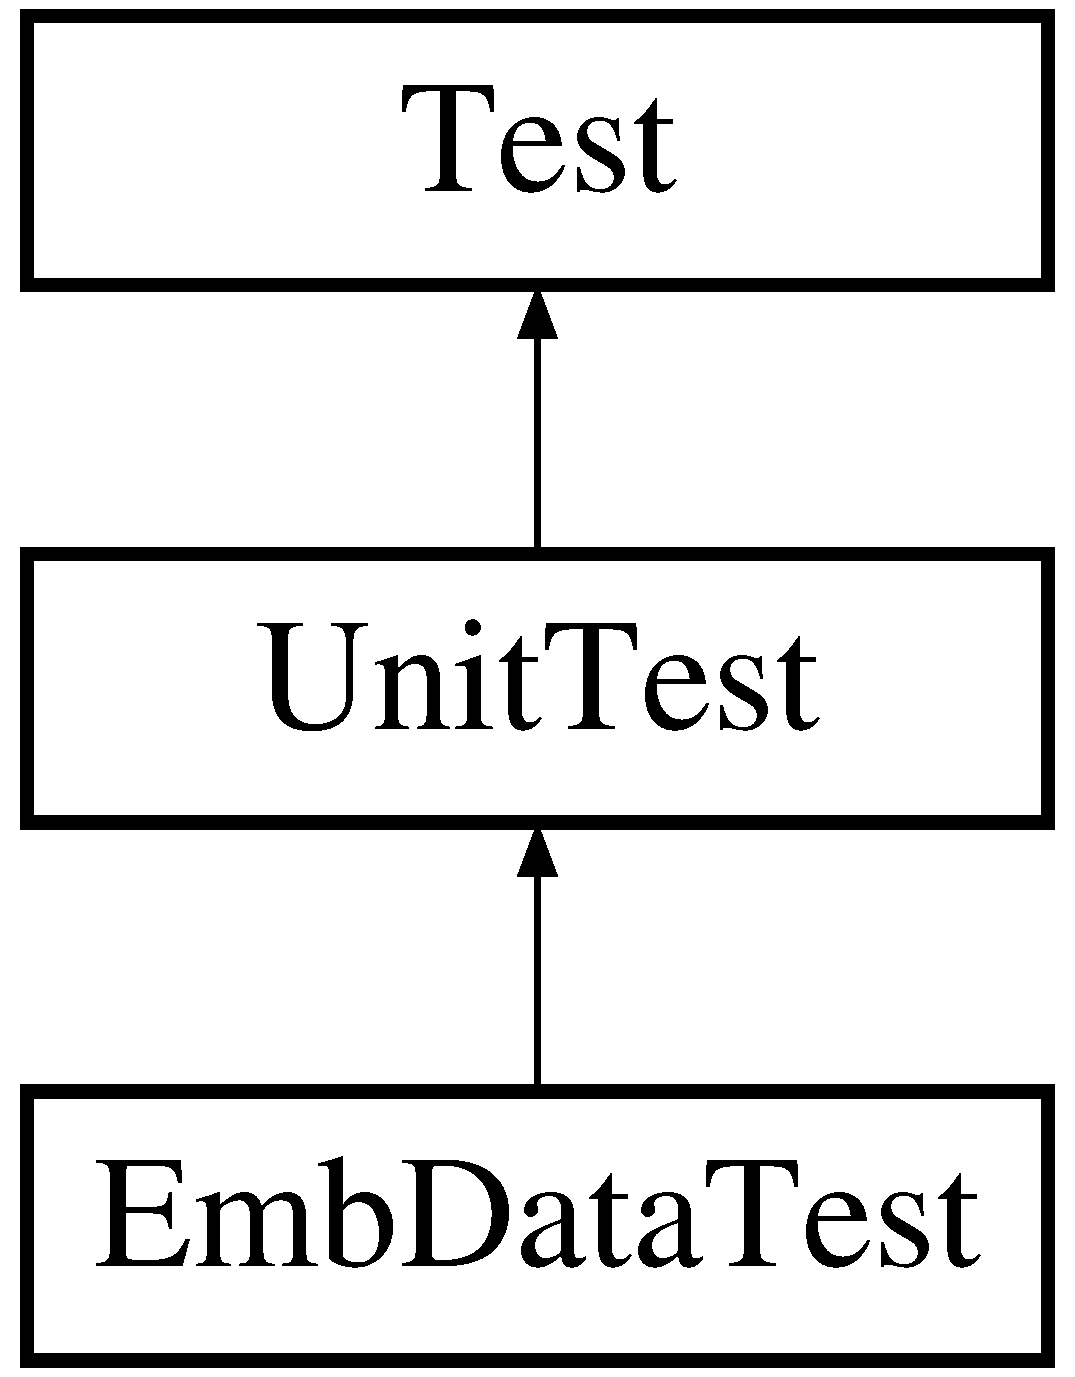
\includegraphics[height=3.000000cm]{classEmbDataTest}
\end{center}
\end{figure}
\subsection*{Public Member Functions}
\begin{DoxyCompactItemize}
\item 
\textbf{ Emb\+Data\+Test} (\textbf{ Test\+Suite} $\ast$s)
\item 
void \textbf{ test\+Embedding} (void)
\item 
void \textbf{ test\+Extracting} (void)
\end{DoxyCompactItemize}
\subsection*{Private Member Functions}
\begin{DoxyCompactItemize}
\item 
bool \textbf{ generic\+Test\+Embedding} (\textbf{ Emb\+Data} emb, \textbf{ Bit\+String} shouldbe)
\item 
bool \textbf{ feed\+\_\+to} (const \textbf{ Bit\+String} \&bs, \textbf{ Emb\+Data} \&emb)
\end{DoxyCompactItemize}
\subsection*{Additional Inherited Members}


\subsection{Constructor \& Destructor Documentation}
\mbox{\label{classEmbDataTest_afe3abb0517e2f92cf4792f91852fc1ed}} 
\index{Emb\+Data\+Test@{Emb\+Data\+Test}!Emb\+Data\+Test@{Emb\+Data\+Test}}
\index{Emb\+Data\+Test@{Emb\+Data\+Test}!Emb\+Data\+Test@{Emb\+Data\+Test}}
\subsubsection{Emb\+Data\+Test()}
{\footnotesize\ttfamily Emb\+Data\+Test\+::\+Emb\+Data\+Test (\begin{DoxyParamCaption}\item[{\textbf{ Test\+Suite} $\ast$}]{s }\end{DoxyParamCaption})}



\subsection{Member Function Documentation}
\mbox{\label{classEmbDataTest_a92f8d6c3c5442152f9b84985607808e0}} 
\index{Emb\+Data\+Test@{Emb\+Data\+Test}!feed\+\_\+to@{feed\+\_\+to}}
\index{feed\+\_\+to@{feed\+\_\+to}!Emb\+Data\+Test@{Emb\+Data\+Test}}
\subsubsection{feed\+\_\+to()}
{\footnotesize\ttfamily bool Emb\+Data\+Test\+::feed\+\_\+to (\begin{DoxyParamCaption}\item[{const \textbf{ Bit\+String} \&}]{bs,  }\item[{\textbf{ Emb\+Data} \&}]{emb }\end{DoxyParamCaption})\hspace{0.3cm}{\ttfamily [private]}}

pass the \doxyref{Bit\+String}{p.}{classBitString} bs to emb using get\+Num\+Bits\+Needed and add\+Bits \begin{DoxyReturn}{Returns}
true iff emb took exactly the (number of) bits from bs 
\end{DoxyReturn}
\mbox{\label{classEmbDataTest_ae153361575be18a44236c1ec69457379}} 
\index{Emb\+Data\+Test@{Emb\+Data\+Test}!generic\+Test\+Embedding@{generic\+Test\+Embedding}}
\index{generic\+Test\+Embedding@{generic\+Test\+Embedding}!Emb\+Data\+Test@{Emb\+Data\+Test}}
\subsubsection{generic\+Test\+Embedding()}
{\footnotesize\ttfamily bool Emb\+Data\+Test\+::generic\+Test\+Embedding (\begin{DoxyParamCaption}\item[{\textbf{ Emb\+Data}}]{emb,  }\item[{\textbf{ Bit\+String}}]{shouldbe }\end{DoxyParamCaption})\hspace{0.3cm}{\ttfamily [private]}}

\mbox{\label{classEmbDataTest_a7748e9d3e1572dfca6577ab909a79869}} 
\index{Emb\+Data\+Test@{Emb\+Data\+Test}!test\+Embedding@{test\+Embedding}}
\index{test\+Embedding@{test\+Embedding}!Emb\+Data\+Test@{Emb\+Data\+Test}}
\subsubsection{test\+Embedding()}
{\footnotesize\ttfamily void Emb\+Data\+Test\+::test\+Embedding (\begin{DoxyParamCaption}\item[{void}]{ }\end{DoxyParamCaption})}

\mbox{\label{classEmbDataTest_a487dab7ea7b62f743c864c52a61e814b}} 
\index{Emb\+Data\+Test@{Emb\+Data\+Test}!test\+Extracting@{test\+Extracting}}
\index{test\+Extracting@{test\+Extracting}!Emb\+Data\+Test@{Emb\+Data\+Test}}
\subsubsection{test\+Extracting()}
{\footnotesize\ttfamily void Emb\+Data\+Test\+::test\+Extracting (\begin{DoxyParamCaption}\item[{void}]{ }\end{DoxyParamCaption})}



The documentation for this class was generated from the following files\+:\begin{DoxyCompactItemize}
\item 
\textbf{ Emb\+Data\+Test.\+h}\item 
\textbf{ Emb\+Data\+Test.\+cc}\end{DoxyCompactItemize}

\section{Embedder Class Reference}
\label{classEmbedder}\index{Embedder@{Embedder}}


{\ttfamily \#include $<$Embedder.\+h$>$}

\subsection*{Public Member Functions}
\begin{DoxyCompactItemize}
\item 
\textbf{ Embedder} (void)
\item 
\textbf{ $\sim$\+Embedder} (void)
\item 
void \textbf{ embed} (void)
\end{DoxyCompactItemize}
\subsection*{Private Member Functions}
\begin{DoxyCompactItemize}
\item 
const \textbf{ Matching} $\ast$ \textbf{ calculate\+Matching} (\textbf{ Progress\+Output} $\ast$prout)
\item 
void \textbf{ embed\+Edge} (\textbf{ Edge} $\ast$e)
\item 
void \textbf{ embed\+Exposed\+Vertex} (\textbf{ Vertex} $\ast$v)
\end{DoxyCompactItemize}
\subsection*{Private Attributes}
\begin{DoxyCompactItemize}
\item 
\textbf{ Bit\+String} \textbf{ To\+Embed}
\end{DoxyCompactItemize}
\subsection*{Static Private Attributes}
\begin{DoxyCompactItemize}
\item 
static const unsigned int \textbf{ Default\+\_\+\+N\+Constr\+Heur} = 1
\end{DoxyCompactItemize}


\subsection{Constructor \& Destructor Documentation}
\mbox{\label{classEmbedder_ad9587f765edd8ae802ba5f4c0c36f627}} 
\index{Embedder@{Embedder}!Embedder@{Embedder}}
\index{Embedder@{Embedder}!Embedder@{Embedder}}
\subsubsection{Embedder()}
{\footnotesize\ttfamily Embedder\+::\+Embedder (\begin{DoxyParamCaption}\item[{void}]{ }\end{DoxyParamCaption})}

\mbox{\label{classEmbedder_aad9422d7eec0e770b1a27e604139fd41}} 
\index{Embedder@{Embedder}!````~Embedder@{$\sim$\+Embedder}}
\index{````~Embedder@{$\sim$\+Embedder}!Embedder@{Embedder}}
\subsubsection{$\sim$\+Embedder()}
{\footnotesize\ttfamily Embedder\+::$\sim$\+Embedder (\begin{DoxyParamCaption}\item[{void}]{ }\end{DoxyParamCaption})}



\subsection{Member Function Documentation}
\mbox{\label{classEmbedder_a5d811c9c54f1e48860052274af0c018b}} 
\index{Embedder@{Embedder}!calculate\+Matching@{calculate\+Matching}}
\index{calculate\+Matching@{calculate\+Matching}!Embedder@{Embedder}}
\subsubsection{calculate\+Matching()}
{\footnotesize\ttfamily const \textbf{ Matching} $\ast$ Embedder\+::calculate\+Matching (\begin{DoxyParamCaption}\item[{\textbf{ Progress\+Output} $\ast$}]{prout }\end{DoxyParamCaption})\hspace{0.3cm}{\ttfamily [private]}}

do the matching algorithms \mbox{\label{classEmbedder_aaef91d4567fb4192c6d9db05eb69cd21}} 
\index{Embedder@{Embedder}!embed@{embed}}
\index{embed@{embed}!Embedder@{Embedder}}
\subsubsection{embed()}
{\footnotesize\ttfamily void Embedder\+::embed (\begin{DoxyParamCaption}\item[{void}]{ }\end{DoxyParamCaption})}

\mbox{\label{classEmbedder_a9f336a582a8008569f9c6a4db2badaa6}} 
\index{Embedder@{Embedder}!embed\+Edge@{embed\+Edge}}
\index{embed\+Edge@{embed\+Edge}!Embedder@{Embedder}}
\subsubsection{embed\+Edge()}
{\footnotesize\ttfamily void Embedder\+::embed\+Edge (\begin{DoxyParamCaption}\item[{\textbf{ Edge} $\ast$}]{e }\end{DoxyParamCaption})\hspace{0.3cm}{\ttfamily [private]}}

embed the two bits represented by the two vertices adjacent to e \mbox{\label{classEmbedder_ac1d1beb28f5bdb0da57c2b698179cf5b}} 
\index{Embedder@{Embedder}!embed\+Exposed\+Vertex@{embed\+Exposed\+Vertex}}
\index{embed\+Exposed\+Vertex@{embed\+Exposed\+Vertex}!Embedder@{Embedder}}
\subsubsection{embed\+Exposed\+Vertex()}
{\footnotesize\ttfamily void Embedder\+::embed\+Exposed\+Vertex (\begin{DoxyParamCaption}\item[{\textbf{ Vertex} $\ast$}]{v }\end{DoxyParamCaption})\hspace{0.3cm}{\ttfamily [private]}}

embed the bit represented by the \doxyref{Vertex}{p.}{classVertex} v 

\subsection{Member Data Documentation}
\mbox{\label{classEmbedder_afc1c21c83bcdc7b265f2433093df85d3}} 
\index{Embedder@{Embedder}!Default\+\_\+\+N\+Constr\+Heur@{Default\+\_\+\+N\+Constr\+Heur}}
\index{Default\+\_\+\+N\+Constr\+Heur@{Default\+\_\+\+N\+Constr\+Heur}!Embedder@{Embedder}}
\subsubsection{Default\+\_\+\+N\+Constr\+Heur}
{\footnotesize\ttfamily const unsigned int Embedder\+::\+Default\+\_\+\+N\+Constr\+Heur = 1\hspace{0.3cm}{\ttfamily [static]}, {\ttfamily [private]}}

\mbox{\label{classEmbedder_a672bcc754465963bb302c94af2e28e61}} 
\index{Embedder@{Embedder}!To\+Embed@{To\+Embed}}
\index{To\+Embed@{To\+Embed}!Embedder@{Embedder}}
\subsubsection{To\+Embed}
{\footnotesize\ttfamily \textbf{ Bit\+String} Embedder\+::\+To\+Embed\hspace{0.3cm}{\ttfamily [private]}}



The documentation for this class was generated from the following files\+:\begin{DoxyCompactItemize}
\item 
\textbf{ Embedder.\+h}\item 
\textbf{ Embedder.\+cc}\end{DoxyCompactItemize}

\section{Encryption\+Algorithm Class Reference}
\label{classEncryptionAlgorithm}\index{Encryption\+Algorithm@{Encryption\+Algorithm}}


{\ttfamily \#include $<$Encryption\+Algorithm.\+h$>$}

\subsection*{Classes}
\begin{DoxyCompactItemize}
\item 
struct \textbf{ struct\+\_\+\+Translation}
\end{DoxyCompactItemize}
\subsection*{Public Types}
\begin{DoxyCompactItemize}
\item 
enum \textbf{ I\+Rep} \{ \newline
\textbf{ N\+O\+NE} = 0, 
\textbf{ T\+W\+O\+F\+I\+SH} = 1, 
\textbf{ R\+I\+J\+N\+D\+A\+E\+L128} = 2, 
\textbf{ R\+I\+J\+N\+D\+A\+E\+L192} = 3, 
\newline
\textbf{ R\+I\+J\+N\+D\+A\+E\+L256} = 4, 
\textbf{ S\+A\+F\+E\+R\+P\+L\+US} = 5, 
\textbf{ R\+C2} = 6, 
\textbf{ X\+T\+EA} = 7, 
\newline
\textbf{ S\+E\+R\+P\+E\+NT} = 8, 
\textbf{ S\+A\+F\+E\+R\+S\+K64} = 9, 
\textbf{ S\+A\+F\+E\+R\+S\+K128} = 10, 
\textbf{ C\+A\+S\+T256} = 11, 
\newline
\textbf{ L\+O\+K\+I97} = 12, 
\textbf{ G\+O\+ST} = 13, 
\textbf{ T\+H\+R\+E\+E\+W\+AY} = 14, 
\textbf{ C\+A\+S\+T128} = 15, 
\newline
\textbf{ B\+L\+O\+W\+F\+I\+SH} = 16, 
\textbf{ D\+ES} = 17, 
\textbf{ T\+R\+I\+P\+L\+E\+D\+ES} = 18, 
\textbf{ E\+N\+I\+G\+MA} = 19, 
\newline
\textbf{ A\+R\+C\+F\+O\+UR} = 20, 
\textbf{ P\+A\+N\+A\+MA} = 21, 
\textbf{ W\+A\+KE} = 22
 \}
\begin{DoxyCompactList}\small\item\em integer representation of encryption algorithm \end{DoxyCompactList}\end{DoxyCompactItemize}
\subsection*{Public Member Functions}
\begin{DoxyCompactItemize}
\item 
\textbf{ Encryption\+Algorithm} (void)
\item 
\textbf{ Encryption\+Algorithm} (\textbf{ I\+Rep} irep)
\item 
\textbf{ Encryption\+Algorithm} (std\+::string srep)
\item 
void \textbf{ set\+Value} (\textbf{ I\+Rep} irep)
\item 
std\+::string \textbf{ get\+String\+Rep} (void) const
\item 
\textbf{ I\+Rep} \textbf{ get\+Integer\+Rep} (void) const
\item 
bool \textbf{ operator==} (const \textbf{ Encryption\+Algorithm} \&algo) const
\end{DoxyCompactItemize}
\subsection*{Static Public Member Functions}
\begin{DoxyCompactItemize}
\item 
static bool \textbf{ is\+Valid\+String\+Rep} (std\+::string srep)
\item 
static bool \textbf{ is\+Valid\+Integer\+Rep} (unsigned int irep)
\item 
static std\+::string \textbf{ translate} (\textbf{ I\+Rep} irep)
\item 
static \textbf{ I\+Rep} \textbf{ translate} (std\+::string srep)
\end{DoxyCompactItemize}
\subsection*{Static Public Attributes}
\begin{DoxyCompactItemize}
\item 
static const unsigned int \textbf{ I\+Rep\+\_\+size} = 5
\begin{DoxyCompactList}\small\item\em number of bits needed to code the algorithm \end{DoxyCompactList}\end{DoxyCompactItemize}
\subsection*{Private Types}
\begin{DoxyCompactItemize}
\item 
typedef struct \textbf{ Encryption\+Algorithm\+::struct\+\_\+\+Translation} \textbf{ Translation}
\end{DoxyCompactItemize}
\subsection*{Private Attributes}
\begin{DoxyCompactItemize}
\item 
\textbf{ I\+Rep} \textbf{ Value}
\end{DoxyCompactItemize}
\subsection*{Static Private Attributes}
\begin{DoxyCompactItemize}
\item 
static const unsigned int \textbf{ Num\+Values} = 23
\item 
static const \textbf{ Translation} \textbf{ Translations} [$\,$]
\end{DoxyCompactItemize}


\subsection{Member Typedef Documentation}
\mbox{\label{classEncryptionAlgorithm_a619b72407ff6ac5ba13c3e50199fc9fa}} 
\index{Encryption\+Algorithm@{Encryption\+Algorithm}!Translation@{Translation}}
\index{Translation@{Translation}!Encryption\+Algorithm@{Encryption\+Algorithm}}
\subsubsection{Translation}
{\footnotesize\ttfamily typedef struct \textbf{ Encryption\+Algorithm\+::struct\+\_\+\+Translation}  \textbf{ Encryption\+Algorithm\+::\+Translation}\hspace{0.3cm}{\ttfamily [private]}}



\subsection{Member Enumeration Documentation}
\mbox{\label{classEncryptionAlgorithm_a0b0a38d56c374dd496b2eb3b196064da}} 
\index{Encryption\+Algorithm@{Encryption\+Algorithm}!I\+Rep@{I\+Rep}}
\index{I\+Rep@{I\+Rep}!Encryption\+Algorithm@{Encryption\+Algorithm}}
\subsubsection{I\+Rep}
{\footnotesize\ttfamily enum \textbf{ Encryption\+Algorithm\+::\+I\+Rep}}

\begin{DoxyEnumFields}{Enumerator}
\raisebox{\heightof{T}}[0pt][0pt]{\index{N\+O\+NE@{N\+O\+NE}!Encryption\+Algorithm@{Encryption\+Algorithm}}\index{Encryption\+Algorithm@{Encryption\+Algorithm}!N\+O\+NE@{N\+O\+NE}}}\mbox{\label{classEncryptionAlgorithm_a0b0a38d56c374dd496b2eb3b196064daa8d4a74a03b2605f7a1f8030a83c9e1e3}} 
N\+O\+NE&\\
\hline

\raisebox{\heightof{T}}[0pt][0pt]{\index{T\+W\+O\+F\+I\+SH@{T\+W\+O\+F\+I\+SH}!Encryption\+Algorithm@{Encryption\+Algorithm}}\index{Encryption\+Algorithm@{Encryption\+Algorithm}!T\+W\+O\+F\+I\+SH@{T\+W\+O\+F\+I\+SH}}}\mbox{\label{classEncryptionAlgorithm_a0b0a38d56c374dd496b2eb3b196064daab720e8b15fef4372ab9393532cb1a13a}} 
T\+W\+O\+F\+I\+SH&\\
\hline

\raisebox{\heightof{T}}[0pt][0pt]{\index{R\+I\+J\+N\+D\+A\+E\+L128@{R\+I\+J\+N\+D\+A\+E\+L128}!Encryption\+Algorithm@{Encryption\+Algorithm}}\index{Encryption\+Algorithm@{Encryption\+Algorithm}!R\+I\+J\+N\+D\+A\+E\+L128@{R\+I\+J\+N\+D\+A\+E\+L128}}}\mbox{\label{classEncryptionAlgorithm_a0b0a38d56c374dd496b2eb3b196064daa443d301831aef540d75c4cf59265d75f}} 
R\+I\+J\+N\+D\+A\+E\+L128&\\
\hline

\raisebox{\heightof{T}}[0pt][0pt]{\index{R\+I\+J\+N\+D\+A\+E\+L192@{R\+I\+J\+N\+D\+A\+E\+L192}!Encryption\+Algorithm@{Encryption\+Algorithm}}\index{Encryption\+Algorithm@{Encryption\+Algorithm}!R\+I\+J\+N\+D\+A\+E\+L192@{R\+I\+J\+N\+D\+A\+E\+L192}}}\mbox{\label{classEncryptionAlgorithm_a0b0a38d56c374dd496b2eb3b196064daa18cddf561172034b88fc5677845de3ff}} 
R\+I\+J\+N\+D\+A\+E\+L192&\\
\hline

\raisebox{\heightof{T}}[0pt][0pt]{\index{R\+I\+J\+N\+D\+A\+E\+L256@{R\+I\+J\+N\+D\+A\+E\+L256}!Encryption\+Algorithm@{Encryption\+Algorithm}}\index{Encryption\+Algorithm@{Encryption\+Algorithm}!R\+I\+J\+N\+D\+A\+E\+L256@{R\+I\+J\+N\+D\+A\+E\+L256}}}\mbox{\label{classEncryptionAlgorithm_a0b0a38d56c374dd496b2eb3b196064daa2f0a09f210fae871590704e1a85cb9f2}} 
R\+I\+J\+N\+D\+A\+E\+L256&\\
\hline

\raisebox{\heightof{T}}[0pt][0pt]{\index{S\+A\+F\+E\+R\+P\+L\+US@{S\+A\+F\+E\+R\+P\+L\+US}!Encryption\+Algorithm@{Encryption\+Algorithm}}\index{Encryption\+Algorithm@{Encryption\+Algorithm}!S\+A\+F\+E\+R\+P\+L\+US@{S\+A\+F\+E\+R\+P\+L\+US}}}\mbox{\label{classEncryptionAlgorithm_a0b0a38d56c374dd496b2eb3b196064daaa9dfea62ff8794811048ddb1032a7071}} 
S\+A\+F\+E\+R\+P\+L\+US&\\
\hline

\raisebox{\heightof{T}}[0pt][0pt]{\index{R\+C2@{R\+C2}!Encryption\+Algorithm@{Encryption\+Algorithm}}\index{Encryption\+Algorithm@{Encryption\+Algorithm}!R\+C2@{R\+C2}}}\mbox{\label{classEncryptionAlgorithm_a0b0a38d56c374dd496b2eb3b196064daa78ad6beefce45cca6430003e49475d95}} 
R\+C2&\\
\hline

\raisebox{\heightof{T}}[0pt][0pt]{\index{X\+T\+EA@{X\+T\+EA}!Encryption\+Algorithm@{Encryption\+Algorithm}}\index{Encryption\+Algorithm@{Encryption\+Algorithm}!X\+T\+EA@{X\+T\+EA}}}\mbox{\label{classEncryptionAlgorithm_a0b0a38d56c374dd496b2eb3b196064daaf542f1648c141ba50cacac5cf590ca00}} 
X\+T\+EA&\\
\hline

\raisebox{\heightof{T}}[0pt][0pt]{\index{S\+E\+R\+P\+E\+NT@{S\+E\+R\+P\+E\+NT}!Encryption\+Algorithm@{Encryption\+Algorithm}}\index{Encryption\+Algorithm@{Encryption\+Algorithm}!S\+E\+R\+P\+E\+NT@{S\+E\+R\+P\+E\+NT}}}\mbox{\label{classEncryptionAlgorithm_a0b0a38d56c374dd496b2eb3b196064daa29333d9a6ebf780ffb67029b841aa5c1}} 
S\+E\+R\+P\+E\+NT&\\
\hline

\raisebox{\heightof{T}}[0pt][0pt]{\index{S\+A\+F\+E\+R\+S\+K64@{S\+A\+F\+E\+R\+S\+K64}!Encryption\+Algorithm@{Encryption\+Algorithm}}\index{Encryption\+Algorithm@{Encryption\+Algorithm}!S\+A\+F\+E\+R\+S\+K64@{S\+A\+F\+E\+R\+S\+K64}}}\mbox{\label{classEncryptionAlgorithm_a0b0a38d56c374dd496b2eb3b196064daa33c11966ccd4075492eede553d34748e}} 
S\+A\+F\+E\+R\+S\+K64&\\
\hline

\raisebox{\heightof{T}}[0pt][0pt]{\index{S\+A\+F\+E\+R\+S\+K128@{S\+A\+F\+E\+R\+S\+K128}!Encryption\+Algorithm@{Encryption\+Algorithm}}\index{Encryption\+Algorithm@{Encryption\+Algorithm}!S\+A\+F\+E\+R\+S\+K128@{S\+A\+F\+E\+R\+S\+K128}}}\mbox{\label{classEncryptionAlgorithm_a0b0a38d56c374dd496b2eb3b196064daad9da67ad1a05fbe2dc7ca6d4ba0a85bd}} 
S\+A\+F\+E\+R\+S\+K128&\\
\hline

\raisebox{\heightof{T}}[0pt][0pt]{\index{C\+A\+S\+T256@{C\+A\+S\+T256}!Encryption\+Algorithm@{Encryption\+Algorithm}}\index{Encryption\+Algorithm@{Encryption\+Algorithm}!C\+A\+S\+T256@{C\+A\+S\+T256}}}\mbox{\label{classEncryptionAlgorithm_a0b0a38d56c374dd496b2eb3b196064daa5da62f3e21e98cf6e04da8636a109536}} 
C\+A\+S\+T256&\\
\hline

\raisebox{\heightof{T}}[0pt][0pt]{\index{L\+O\+K\+I97@{L\+O\+K\+I97}!Encryption\+Algorithm@{Encryption\+Algorithm}}\index{Encryption\+Algorithm@{Encryption\+Algorithm}!L\+O\+K\+I97@{L\+O\+K\+I97}}}\mbox{\label{classEncryptionAlgorithm_a0b0a38d56c374dd496b2eb3b196064daac83d0354296871b8f1d6d16e15967245}} 
L\+O\+K\+I97&\\
\hline

\raisebox{\heightof{T}}[0pt][0pt]{\index{G\+O\+ST@{G\+O\+ST}!Encryption\+Algorithm@{Encryption\+Algorithm}}\index{Encryption\+Algorithm@{Encryption\+Algorithm}!G\+O\+ST@{G\+O\+ST}}}\mbox{\label{classEncryptionAlgorithm_a0b0a38d56c374dd496b2eb3b196064daa01e07af2d40a0b0bb0dd68a653be7f48}} 
G\+O\+ST&\\
\hline

\raisebox{\heightof{T}}[0pt][0pt]{\index{T\+H\+R\+E\+E\+W\+AY@{T\+H\+R\+E\+E\+W\+AY}!Encryption\+Algorithm@{Encryption\+Algorithm}}\index{Encryption\+Algorithm@{Encryption\+Algorithm}!T\+H\+R\+E\+E\+W\+AY@{T\+H\+R\+E\+E\+W\+AY}}}\mbox{\label{classEncryptionAlgorithm_a0b0a38d56c374dd496b2eb3b196064daa87b9713f03f6d386a291adce770997d5}} 
T\+H\+R\+E\+E\+W\+AY&\\
\hline

\raisebox{\heightof{T}}[0pt][0pt]{\index{C\+A\+S\+T128@{C\+A\+S\+T128}!Encryption\+Algorithm@{Encryption\+Algorithm}}\index{Encryption\+Algorithm@{Encryption\+Algorithm}!C\+A\+S\+T128@{C\+A\+S\+T128}}}\mbox{\label{classEncryptionAlgorithm_a0b0a38d56c374dd496b2eb3b196064daad515a7dc78cbd5612e83a9aae1107244}} 
C\+A\+S\+T128&\\
\hline

\raisebox{\heightof{T}}[0pt][0pt]{\index{B\+L\+O\+W\+F\+I\+SH@{B\+L\+O\+W\+F\+I\+SH}!Encryption\+Algorithm@{Encryption\+Algorithm}}\index{Encryption\+Algorithm@{Encryption\+Algorithm}!B\+L\+O\+W\+F\+I\+SH@{B\+L\+O\+W\+F\+I\+SH}}}\mbox{\label{classEncryptionAlgorithm_a0b0a38d56c374dd496b2eb3b196064daa0d677fe184757e7586de175698103a03}} 
B\+L\+O\+W\+F\+I\+SH&\\
\hline

\raisebox{\heightof{T}}[0pt][0pt]{\index{D\+ES@{D\+ES}!Encryption\+Algorithm@{Encryption\+Algorithm}}\index{Encryption\+Algorithm@{Encryption\+Algorithm}!D\+ES@{D\+ES}}}\mbox{\label{classEncryptionAlgorithm_a0b0a38d56c374dd496b2eb3b196064daa9cee17436bacf6fb196fa9314eb36e86}} 
D\+ES&\\
\hline

\raisebox{\heightof{T}}[0pt][0pt]{\index{T\+R\+I\+P\+L\+E\+D\+ES@{T\+R\+I\+P\+L\+E\+D\+ES}!Encryption\+Algorithm@{Encryption\+Algorithm}}\index{Encryption\+Algorithm@{Encryption\+Algorithm}!T\+R\+I\+P\+L\+E\+D\+ES@{T\+R\+I\+P\+L\+E\+D\+ES}}}\mbox{\label{classEncryptionAlgorithm_a0b0a38d56c374dd496b2eb3b196064daa1a2a0556c135deea10e369fbac503d23}} 
T\+R\+I\+P\+L\+E\+D\+ES&\\
\hline

\raisebox{\heightof{T}}[0pt][0pt]{\index{E\+N\+I\+G\+MA@{E\+N\+I\+G\+MA}!Encryption\+Algorithm@{Encryption\+Algorithm}}\index{Encryption\+Algorithm@{Encryption\+Algorithm}!E\+N\+I\+G\+MA@{E\+N\+I\+G\+MA}}}\mbox{\label{classEncryptionAlgorithm_a0b0a38d56c374dd496b2eb3b196064daa8b222ca28b942be68840b02dded149ff}} 
E\+N\+I\+G\+MA&\\
\hline

\raisebox{\heightof{T}}[0pt][0pt]{\index{A\+R\+C\+F\+O\+UR@{A\+R\+C\+F\+O\+UR}!Encryption\+Algorithm@{Encryption\+Algorithm}}\index{Encryption\+Algorithm@{Encryption\+Algorithm}!A\+R\+C\+F\+O\+UR@{A\+R\+C\+F\+O\+UR}}}\mbox{\label{classEncryptionAlgorithm_a0b0a38d56c374dd496b2eb3b196064daa9b6958d25a21123bb63d2080fa8064b5}} 
A\+R\+C\+F\+O\+UR&\\
\hline

\raisebox{\heightof{T}}[0pt][0pt]{\index{P\+A\+N\+A\+MA@{P\+A\+N\+A\+MA}!Encryption\+Algorithm@{Encryption\+Algorithm}}\index{Encryption\+Algorithm@{Encryption\+Algorithm}!P\+A\+N\+A\+MA@{P\+A\+N\+A\+MA}}}\mbox{\label{classEncryptionAlgorithm_a0b0a38d56c374dd496b2eb3b196064daae9dfbc00d41cf18d6a765c5014a5989e}} 
P\+A\+N\+A\+MA&\\
\hline

\raisebox{\heightof{T}}[0pt][0pt]{\index{W\+A\+KE@{W\+A\+KE}!Encryption\+Algorithm@{Encryption\+Algorithm}}\index{Encryption\+Algorithm@{Encryption\+Algorithm}!W\+A\+KE@{W\+A\+KE}}}\mbox{\label{classEncryptionAlgorithm_a0b0a38d56c374dd496b2eb3b196064daa8bac05b1857afecc3d189a61a61d4923}} 
W\+A\+KE&\\
\hline

\end{DoxyEnumFields}


\subsection{Constructor \& Destructor Documentation}
\mbox{\label{classEncryptionAlgorithm_a8153a4eeaf5463cdb05f0715fe782a1d}} 
\index{Encryption\+Algorithm@{Encryption\+Algorithm}!Encryption\+Algorithm@{Encryption\+Algorithm}}
\index{Encryption\+Algorithm@{Encryption\+Algorithm}!Encryption\+Algorithm@{Encryption\+Algorithm}}
\subsubsection{Encryption\+Algorithm()\hspace{0.1cm}{\footnotesize\ttfamily [1/3]}}
{\footnotesize\ttfamily Encryption\+Algorithm\+::\+Encryption\+Algorithm (\begin{DoxyParamCaption}\item[{void}]{ }\end{DoxyParamCaption})}

\mbox{\label{classEncryptionAlgorithm_ac0c8f868b64367f33cabbfdb38c5ff23}} 
\index{Encryption\+Algorithm@{Encryption\+Algorithm}!Encryption\+Algorithm@{Encryption\+Algorithm}}
\index{Encryption\+Algorithm@{Encryption\+Algorithm}!Encryption\+Algorithm@{Encryption\+Algorithm}}
\subsubsection{Encryption\+Algorithm()\hspace{0.1cm}{\footnotesize\ttfamily [2/3]}}
{\footnotesize\ttfamily Encryption\+Algorithm\+::\+Encryption\+Algorithm (\begin{DoxyParamCaption}\item[{\textbf{ Encryption\+Algorithm\+::\+I\+Rep}}]{irep }\end{DoxyParamCaption})}

\mbox{\label{classEncryptionAlgorithm_a940896eedb7cecc898d1e7630d11c650}} 
\index{Encryption\+Algorithm@{Encryption\+Algorithm}!Encryption\+Algorithm@{Encryption\+Algorithm}}
\index{Encryption\+Algorithm@{Encryption\+Algorithm}!Encryption\+Algorithm@{Encryption\+Algorithm}}
\subsubsection{Encryption\+Algorithm()\hspace{0.1cm}{\footnotesize\ttfamily [3/3]}}
{\footnotesize\ttfamily Encryption\+Algorithm\+::\+Encryption\+Algorithm (\begin{DoxyParamCaption}\item[{std\+::string}]{srep }\end{DoxyParamCaption})}

construct a new \doxyref{Encryption\+Algorithm}{p.}{classEncryptionAlgorithm} object from a std\+::string representation 
\begin{DoxyParams}{Parameters}
{\em srep} & a valid(!) std\+::string representation \\
\hline
\end{DoxyParams}


\subsection{Member Function Documentation}
\mbox{\label{classEncryptionAlgorithm_a45524ec1f2d469ac1c3e2a62b407d6b3}} 
\index{Encryption\+Algorithm@{Encryption\+Algorithm}!get\+Integer\+Rep@{get\+Integer\+Rep}}
\index{get\+Integer\+Rep@{get\+Integer\+Rep}!Encryption\+Algorithm@{Encryption\+Algorithm}}
\subsubsection{get\+Integer\+Rep()}
{\footnotesize\ttfamily \textbf{ Encryption\+Algorithm\+::\+I\+Rep} Encryption\+Algorithm\+::get\+Integer\+Rep (\begin{DoxyParamCaption}\item[{void}]{ }\end{DoxyParamCaption}) const}

\mbox{\label{classEncryptionAlgorithm_aeb9d69a2abdf02658ccf410f3fa93239}} 
\index{Encryption\+Algorithm@{Encryption\+Algorithm}!get\+String\+Rep@{get\+String\+Rep}}
\index{get\+String\+Rep@{get\+String\+Rep}!Encryption\+Algorithm@{Encryption\+Algorithm}}
\subsubsection{get\+String\+Rep()}
{\footnotesize\ttfamily std\+::string Encryption\+Algorithm\+::get\+String\+Rep (\begin{DoxyParamCaption}\item[{void}]{ }\end{DoxyParamCaption}) const}

\mbox{\label{classEncryptionAlgorithm_a6831aa0c243e97fea301b9941e80ff54}} 
\index{Encryption\+Algorithm@{Encryption\+Algorithm}!is\+Valid\+Integer\+Rep@{is\+Valid\+Integer\+Rep}}
\index{is\+Valid\+Integer\+Rep@{is\+Valid\+Integer\+Rep}!Encryption\+Algorithm@{Encryption\+Algorithm}}
\subsubsection{is\+Valid\+Integer\+Rep()}
{\footnotesize\ttfamily bool Encryption\+Algorithm\+::is\+Valid\+Integer\+Rep (\begin{DoxyParamCaption}\item[{unsigned int}]{irep }\end{DoxyParamCaption})\hspace{0.3cm}{\ttfamily [static]}}

\mbox{\label{classEncryptionAlgorithm_aa27946ca69ace48b6264fcd6a11bf820}} 
\index{Encryption\+Algorithm@{Encryption\+Algorithm}!is\+Valid\+String\+Rep@{is\+Valid\+String\+Rep}}
\index{is\+Valid\+String\+Rep@{is\+Valid\+String\+Rep}!Encryption\+Algorithm@{Encryption\+Algorithm}}
\subsubsection{is\+Valid\+String\+Rep()}
{\footnotesize\ttfamily bool Encryption\+Algorithm\+::is\+Valid\+String\+Rep (\begin{DoxyParamCaption}\item[{std\+::string}]{srep }\end{DoxyParamCaption})\hspace{0.3cm}{\ttfamily [static]}}

check if srep is a valid std\+::string representation (w.\+r.\+t the Translations array) 
\begin{DoxyParams}{Parameters}
{\em srep} & a std\+::string that maybe represents an encryption algorithm fron the Translations table \\
\hline
\end{DoxyParams}
\begin{DoxyReturn}{Returns}
true iff the Translations table contains srep 
\end{DoxyReturn}
\mbox{\label{classEncryptionAlgorithm_a62450c1dbf1e0a539b1077b50dfc9369}} 
\index{Encryption\+Algorithm@{Encryption\+Algorithm}!operator==@{operator==}}
\index{operator==@{operator==}!Encryption\+Algorithm@{Encryption\+Algorithm}}
\subsubsection{operator==()}
{\footnotesize\ttfamily bool Encryption\+Algorithm\+::operator== (\begin{DoxyParamCaption}\item[{const \textbf{ Encryption\+Algorithm} \&}]{algo }\end{DoxyParamCaption}) const\hspace{0.3cm}{\ttfamily [inline]}}

\mbox{\label{classEncryptionAlgorithm_a5fe2a9ccaeb63a6d24e9c6c826aa0aec}} 
\index{Encryption\+Algorithm@{Encryption\+Algorithm}!set\+Value@{set\+Value}}
\index{set\+Value@{set\+Value}!Encryption\+Algorithm@{Encryption\+Algorithm}}
\subsubsection{set\+Value()}
{\footnotesize\ttfamily void Encryption\+Algorithm\+::set\+Value (\begin{DoxyParamCaption}\item[{\textbf{ Encryption\+Algorithm\+::\+I\+Rep}}]{irep }\end{DoxyParamCaption})}

\mbox{\label{classEncryptionAlgorithm_a11940db2351b1c3bb112e82584db3ce2}} 
\index{Encryption\+Algorithm@{Encryption\+Algorithm}!translate@{translate}}
\index{translate@{translate}!Encryption\+Algorithm@{Encryption\+Algorithm}}
\subsubsection{translate()\hspace{0.1cm}{\footnotesize\ttfamily [1/2]}}
{\footnotesize\ttfamily std\+::string Encryption\+Algorithm\+::translate (\begin{DoxyParamCaption}\item[{\textbf{ Encryption\+Algorithm\+::\+I\+Rep}}]{irep }\end{DoxyParamCaption})\hspace{0.3cm}{\ttfamily [static]}}

translate an integer representation into the corresponding std\+::string representation \mbox{\label{classEncryptionAlgorithm_a3553b82544a11b6cd730489bf62493b9}} 
\index{Encryption\+Algorithm@{Encryption\+Algorithm}!translate@{translate}}
\index{translate@{translate}!Encryption\+Algorithm@{Encryption\+Algorithm}}
\subsubsection{translate()\hspace{0.1cm}{\footnotesize\ttfamily [2/2]}}
{\footnotesize\ttfamily \textbf{ Encryption\+Algorithm\+::\+I\+Rep} Encryption\+Algorithm\+::translate (\begin{DoxyParamCaption}\item[{std\+::string}]{srep }\end{DoxyParamCaption})\hspace{0.3cm}{\ttfamily [static]}}

translate a valid std\+::string representation into the corresponding integer representation 

\subsection{Member Data Documentation}
\mbox{\label{classEncryptionAlgorithm_a6c180bb36ea4f6cedbb1b6e0817c5aee}} 
\index{Encryption\+Algorithm@{Encryption\+Algorithm}!I\+Rep\+\_\+size@{I\+Rep\+\_\+size}}
\index{I\+Rep\+\_\+size@{I\+Rep\+\_\+size}!Encryption\+Algorithm@{Encryption\+Algorithm}}
\subsubsection{I\+Rep\+\_\+size}
{\footnotesize\ttfamily const unsigned int Encryption\+Algorithm\+::\+I\+Rep\+\_\+size = 5\hspace{0.3cm}{\ttfamily [static]}}

\mbox{\label{classEncryptionAlgorithm_ac73bd3dce21f67281d56d2f472cae216}} 
\index{Encryption\+Algorithm@{Encryption\+Algorithm}!Num\+Values@{Num\+Values}}
\index{Num\+Values@{Num\+Values}!Encryption\+Algorithm@{Encryption\+Algorithm}}
\subsubsection{Num\+Values}
{\footnotesize\ttfamily const unsigned int Encryption\+Algorithm\+::\+Num\+Values = 23\hspace{0.3cm}{\ttfamily [static]}, {\ttfamily [private]}}

\mbox{\label{classEncryptionAlgorithm_a04ae419348583b3a689f04877968ea06}} 
\index{Encryption\+Algorithm@{Encryption\+Algorithm}!Translations@{Translations}}
\index{Translations@{Translations}!Encryption\+Algorithm@{Encryption\+Algorithm}}
\subsubsection{Translations}
{\footnotesize\ttfamily const \textbf{ Encryption\+Algorithm\+::\+Translation} Encryption\+Algorithm\+::\+Translations\hspace{0.3cm}{\ttfamily [static]}, {\ttfamily [private]}}

{\bfseries Initial value\+:}
\begin{DoxyCode}
= \{
        \{ NONE, \textcolor{stringliteral}{"none"} \},
        \{ TWOFISH, \textcolor{stringliteral}{"twofish"} \},
        \{ RIJNDAEL128, \textcolor{stringliteral}{"rijndael-128"} \},
        \{ RIJNDAEL192, \textcolor{stringliteral}{"rijndael-192"} \},
        \{ RIJNDAEL256, \textcolor{stringliteral}{"rijndael-256"} \},
        \{ SAFERPLUS, \textcolor{stringliteral}{"saferplus"} \},
        \{ RC2, \textcolor{stringliteral}{"rc2"} \},
        \{ XTEA, \textcolor{stringliteral}{"xtea"} \},
        \{ SERPENT, \textcolor{stringliteral}{"serpent"} \},
        \{ SAFERSK64, \textcolor{stringliteral}{"safer-sk64"} \},
        \{ SAFERSK128, \textcolor{stringliteral}{"safer-sk128"} \},
        \{ CAST256, \textcolor{stringliteral}{"cast-256"} \},
        \{ LOKI97, \textcolor{stringliteral}{"loki97"} \},
        \{ GOST, \textcolor{stringliteral}{"gost"} \},
        \{ THREEWAY, \textcolor{stringliteral}{"threeway"} \},
        \{ CAST128, \textcolor{stringliteral}{"cast-128"} \},
        \{ BLOWFISH, \textcolor{stringliteral}{"blowfish"} \},
        \{ DES, \textcolor{stringliteral}{"des"} \},
        \{ TRIPLEDES, \textcolor{stringliteral}{"tripledes"} \},
        \{ ENIGMA, \textcolor{stringliteral}{"enigma"} \},
        \{ ARCFOUR, \textcolor{stringliteral}{"arcfour"} \},
        \{ PANAMA, \textcolor{stringliteral}{"panama"} \},
        \{ WAKE, \textcolor{stringliteral}{"wake"} \}
\}
\end{DoxyCode}
\mbox{\label{classEncryptionAlgorithm_af75d13966d2b849cb0d92446ab982f5a}} 
\index{Encryption\+Algorithm@{Encryption\+Algorithm}!Value@{Value}}
\index{Value@{Value}!Encryption\+Algorithm@{Encryption\+Algorithm}}
\subsubsection{Value}
{\footnotesize\ttfamily \textbf{ I\+Rep} Encryption\+Algorithm\+::\+Value\hspace{0.3cm}{\ttfamily [private]}}



The documentation for this class was generated from the following files\+:\begin{DoxyCompactItemize}
\item 
\textbf{ Encryption\+Algorithm.\+h}\item 
\textbf{ Encryption\+Algorithm.\+cc}\end{DoxyCompactItemize}

\section{Encryption\+Mode Class Reference}
\label{classEncryptionMode}\index{Encryption\+Mode@{Encryption\+Mode}}


{\ttfamily \#include $<$Encryption\+Mode.\+h$>$}

\subsection*{Classes}
\begin{DoxyCompactItemize}
\item 
struct \textbf{ struct\+\_\+\+Translation}
\end{DoxyCompactItemize}
\subsection*{Public Types}
\begin{DoxyCompactItemize}
\item 
enum \textbf{ I\+Rep} \{ \newline
\textbf{ E\+CB} = 0, 
\textbf{ C\+BC} = 1, 
\textbf{ O\+FB} = 2, 
\textbf{ C\+FB} = 3, 
\newline
\textbf{ N\+O\+FB} = 4, 
\textbf{ N\+C\+FB} = 5, 
\textbf{ C\+TR} = 6, 
\textbf{ S\+T\+R\+E\+AM} = 7
 \}
\begin{DoxyCompactList}\small\item\em integer representation of encryption mode \end{DoxyCompactList}\end{DoxyCompactItemize}
\subsection*{Public Member Functions}
\begin{DoxyCompactItemize}
\item 
\textbf{ Encryption\+Mode} (void)
\item 
\textbf{ Encryption\+Mode} (\textbf{ I\+Rep} irep)
\item 
\textbf{ Encryption\+Mode} (std\+::string srep)
\item 
void \textbf{ set\+Value} (\textbf{ I\+Rep} irep)
\item 
std\+::string \textbf{ get\+String\+Rep} (void) const
\item 
\textbf{ I\+Rep} \textbf{ get\+Integer\+Rep} (void) const
\item 
bool \textbf{ operator==} (const \textbf{ Encryption\+Mode} \&mode) const
\end{DoxyCompactItemize}
\subsection*{Static Public Member Functions}
\begin{DoxyCompactItemize}
\item 
static bool \textbf{ is\+Valid\+String\+Rep} (std\+::string srep)
\item 
static bool \textbf{ is\+Valid\+Integer\+Rep} (unsigned int irep)
\item 
static std\+::string \textbf{ translate} (\textbf{ I\+Rep} irep)
\item 
static \textbf{ I\+Rep} \textbf{ translate} (std\+::string srep)
\end{DoxyCompactItemize}
\subsection*{Static Public Attributes}
\begin{DoxyCompactItemize}
\item 
static const unsigned int \textbf{ I\+Rep\+\_\+size} = 3
\begin{DoxyCompactList}\small\item\em number of bits needed to code the mode \end{DoxyCompactList}\end{DoxyCompactItemize}
\subsection*{Private Types}
\begin{DoxyCompactItemize}
\item 
typedef struct \textbf{ Encryption\+Mode\+::struct\+\_\+\+Translation} \textbf{ Translation}
\end{DoxyCompactItemize}
\subsection*{Private Attributes}
\begin{DoxyCompactItemize}
\item 
\textbf{ I\+Rep} \textbf{ Value}
\end{DoxyCompactItemize}
\subsection*{Static Private Attributes}
\begin{DoxyCompactItemize}
\item 
static const unsigned int \textbf{ Num\+Values} = 8
\item 
static const \textbf{ Translation} \textbf{ Translations} [$\,$]
\end{DoxyCompactItemize}


\subsection{Member Typedef Documentation}
\mbox{\label{classEncryptionMode_a2cc1860b5cc1e1fadf7ba0067a903405}} 
\index{Encryption\+Mode@{Encryption\+Mode}!Translation@{Translation}}
\index{Translation@{Translation}!Encryption\+Mode@{Encryption\+Mode}}
\subsubsection{Translation}
{\footnotesize\ttfamily typedef struct \textbf{ Encryption\+Mode\+::struct\+\_\+\+Translation}  \textbf{ Encryption\+Mode\+::\+Translation}\hspace{0.3cm}{\ttfamily [private]}}



\subsection{Member Enumeration Documentation}
\mbox{\label{classEncryptionMode_a136e2b84c94488c7f0fe4c2c781b1581}} 
\index{Encryption\+Mode@{Encryption\+Mode}!I\+Rep@{I\+Rep}}
\index{I\+Rep@{I\+Rep}!Encryption\+Mode@{Encryption\+Mode}}
\subsubsection{I\+Rep}
{\footnotesize\ttfamily enum \textbf{ Encryption\+Mode\+::\+I\+Rep}}

\begin{DoxyEnumFields}{Enumerator}
\raisebox{\heightof{T}}[0pt][0pt]{\index{E\+CB@{E\+CB}!Encryption\+Mode@{Encryption\+Mode}}\index{Encryption\+Mode@{Encryption\+Mode}!E\+CB@{E\+CB}}}\mbox{\label{classEncryptionMode_a136e2b84c94488c7f0fe4c2c781b1581ac08a5875339f740132386b99b8262a23}} 
E\+CB&\\
\hline

\raisebox{\heightof{T}}[0pt][0pt]{\index{C\+BC@{C\+BC}!Encryption\+Mode@{Encryption\+Mode}}\index{Encryption\+Mode@{Encryption\+Mode}!C\+BC@{C\+BC}}}\mbox{\label{classEncryptionMode_a136e2b84c94488c7f0fe4c2c781b1581a3c5b2f7f95ff4b1613687119248ab96d}} 
C\+BC&\\
\hline

\raisebox{\heightof{T}}[0pt][0pt]{\index{O\+FB@{O\+FB}!Encryption\+Mode@{Encryption\+Mode}}\index{Encryption\+Mode@{Encryption\+Mode}!O\+FB@{O\+FB}}}\mbox{\label{classEncryptionMode_a136e2b84c94488c7f0fe4c2c781b1581a1a6e3391aab5f3c35ff71f4e89875b74}} 
O\+FB&\\
\hline

\raisebox{\heightof{T}}[0pt][0pt]{\index{C\+FB@{C\+FB}!Encryption\+Mode@{Encryption\+Mode}}\index{Encryption\+Mode@{Encryption\+Mode}!C\+FB@{C\+FB}}}\mbox{\label{classEncryptionMode_a136e2b84c94488c7f0fe4c2c781b1581a01a6f1542ff51301bc2f909bdcac5e92}} 
C\+FB&\\
\hline

\raisebox{\heightof{T}}[0pt][0pt]{\index{N\+O\+FB@{N\+O\+FB}!Encryption\+Mode@{Encryption\+Mode}}\index{Encryption\+Mode@{Encryption\+Mode}!N\+O\+FB@{N\+O\+FB}}}\mbox{\label{classEncryptionMode_a136e2b84c94488c7f0fe4c2c781b1581ac8bfd5ef69e4edf2cd934fd61c26d691}} 
N\+O\+FB&\\
\hline

\raisebox{\heightof{T}}[0pt][0pt]{\index{N\+C\+FB@{N\+C\+FB}!Encryption\+Mode@{Encryption\+Mode}}\index{Encryption\+Mode@{Encryption\+Mode}!N\+C\+FB@{N\+C\+FB}}}\mbox{\label{classEncryptionMode_a136e2b84c94488c7f0fe4c2c781b1581a41e9989ca9de600aee36c4c41271d331}} 
N\+C\+FB&\\
\hline

\raisebox{\heightof{T}}[0pt][0pt]{\index{C\+TR@{C\+TR}!Encryption\+Mode@{Encryption\+Mode}}\index{Encryption\+Mode@{Encryption\+Mode}!C\+TR@{C\+TR}}}\mbox{\label{classEncryptionMode_a136e2b84c94488c7f0fe4c2c781b1581aab9094135177237ba8f9e1960a02d391}} 
C\+TR&\\
\hline

\raisebox{\heightof{T}}[0pt][0pt]{\index{S\+T\+R\+E\+AM@{S\+T\+R\+E\+AM}!Encryption\+Mode@{Encryption\+Mode}}\index{Encryption\+Mode@{Encryption\+Mode}!S\+T\+R\+E\+AM@{S\+T\+R\+E\+AM}}}\mbox{\label{classEncryptionMode_a136e2b84c94488c7f0fe4c2c781b1581a27cbbe34c17df2bbe2d7fca18fe44373}} 
S\+T\+R\+E\+AM&\\
\hline

\end{DoxyEnumFields}


\subsection{Constructor \& Destructor Documentation}
\mbox{\label{classEncryptionMode_a2c228ca6820b76748d84e04828e2c38c}} 
\index{Encryption\+Mode@{Encryption\+Mode}!Encryption\+Mode@{Encryption\+Mode}}
\index{Encryption\+Mode@{Encryption\+Mode}!Encryption\+Mode@{Encryption\+Mode}}
\subsubsection{Encryption\+Mode()\hspace{0.1cm}{\footnotesize\ttfamily [1/3]}}
{\footnotesize\ttfamily Encryption\+Mode\+::\+Encryption\+Mode (\begin{DoxyParamCaption}\item[{void}]{ }\end{DoxyParamCaption})}

construct a new \doxyref{Encryption\+Mode}{p.}{classEncryptionMode} object setting Value to E\+CB \mbox{\label{classEncryptionMode_abcb7fda77b5f7ab31a4a26c788ae35d9}} 
\index{Encryption\+Mode@{Encryption\+Mode}!Encryption\+Mode@{Encryption\+Mode}}
\index{Encryption\+Mode@{Encryption\+Mode}!Encryption\+Mode@{Encryption\+Mode}}
\subsubsection{Encryption\+Mode()\hspace{0.1cm}{\footnotesize\ttfamily [2/3]}}
{\footnotesize\ttfamily Encryption\+Mode\+::\+Encryption\+Mode (\begin{DoxyParamCaption}\item[{\textbf{ Encryption\+Mode\+::\+I\+Rep}}]{irep }\end{DoxyParamCaption})}

\mbox{\label{classEncryptionMode_a74bca6f0a7c1ceec56f368fa77d33c07}} 
\index{Encryption\+Mode@{Encryption\+Mode}!Encryption\+Mode@{Encryption\+Mode}}
\index{Encryption\+Mode@{Encryption\+Mode}!Encryption\+Mode@{Encryption\+Mode}}
\subsubsection{Encryption\+Mode()\hspace{0.1cm}{\footnotesize\ttfamily [3/3]}}
{\footnotesize\ttfamily Encryption\+Mode\+::\+Encryption\+Mode (\begin{DoxyParamCaption}\item[{std\+::string}]{srep }\end{DoxyParamCaption})}

construct a new \doxyref{Encryption\+Mode}{p.}{classEncryptionMode} object from a std\+::string representation 
\begin{DoxyParams}{Parameters}
{\em srep} & a valid(!) std\+::string representation \\
\hline
\end{DoxyParams}


\subsection{Member Function Documentation}
\mbox{\label{classEncryptionMode_af4a17e17a48c6a86ddda108227424c38}} 
\index{Encryption\+Mode@{Encryption\+Mode}!get\+Integer\+Rep@{get\+Integer\+Rep}}
\index{get\+Integer\+Rep@{get\+Integer\+Rep}!Encryption\+Mode@{Encryption\+Mode}}
\subsubsection{get\+Integer\+Rep()}
{\footnotesize\ttfamily \textbf{ Encryption\+Mode\+::\+I\+Rep} Encryption\+Mode\+::get\+Integer\+Rep (\begin{DoxyParamCaption}\item[{void}]{ }\end{DoxyParamCaption}) const}

\mbox{\label{classEncryptionMode_a6ed8917f0a8f5e41e39e877ce6a1966c}} 
\index{Encryption\+Mode@{Encryption\+Mode}!get\+String\+Rep@{get\+String\+Rep}}
\index{get\+String\+Rep@{get\+String\+Rep}!Encryption\+Mode@{Encryption\+Mode}}
\subsubsection{get\+String\+Rep()}
{\footnotesize\ttfamily std\+::string Encryption\+Mode\+::get\+String\+Rep (\begin{DoxyParamCaption}\item[{void}]{ }\end{DoxyParamCaption}) const}

\mbox{\label{classEncryptionMode_a4148d3e25613ba8733bbc459805c71d0}} 
\index{Encryption\+Mode@{Encryption\+Mode}!is\+Valid\+Integer\+Rep@{is\+Valid\+Integer\+Rep}}
\index{is\+Valid\+Integer\+Rep@{is\+Valid\+Integer\+Rep}!Encryption\+Mode@{Encryption\+Mode}}
\subsubsection{is\+Valid\+Integer\+Rep()}
{\footnotesize\ttfamily bool Encryption\+Mode\+::is\+Valid\+Integer\+Rep (\begin{DoxyParamCaption}\item[{unsigned int}]{irep }\end{DoxyParamCaption})\hspace{0.3cm}{\ttfamily [static]}}

\mbox{\label{classEncryptionMode_a3fe8eeb1fb6397fcb14bd7964d0a3dbf}} 
\index{Encryption\+Mode@{Encryption\+Mode}!is\+Valid\+String\+Rep@{is\+Valid\+String\+Rep}}
\index{is\+Valid\+String\+Rep@{is\+Valid\+String\+Rep}!Encryption\+Mode@{Encryption\+Mode}}
\subsubsection{is\+Valid\+String\+Rep()}
{\footnotesize\ttfamily bool Encryption\+Mode\+::is\+Valid\+String\+Rep (\begin{DoxyParamCaption}\item[{std\+::string}]{srep }\end{DoxyParamCaption})\hspace{0.3cm}{\ttfamily [static]}}

\mbox{\label{classEncryptionMode_a7f5159af8571867c3204763927468254}} 
\index{Encryption\+Mode@{Encryption\+Mode}!operator==@{operator==}}
\index{operator==@{operator==}!Encryption\+Mode@{Encryption\+Mode}}
\subsubsection{operator==()}
{\footnotesize\ttfamily bool Encryption\+Mode\+::operator== (\begin{DoxyParamCaption}\item[{const \textbf{ Encryption\+Mode} \&}]{mode }\end{DoxyParamCaption}) const\hspace{0.3cm}{\ttfamily [inline]}}

\mbox{\label{classEncryptionMode_a166b3995fdb42166bde42d52cc92a94b}} 
\index{Encryption\+Mode@{Encryption\+Mode}!set\+Value@{set\+Value}}
\index{set\+Value@{set\+Value}!Encryption\+Mode@{Encryption\+Mode}}
\subsubsection{set\+Value()}
{\footnotesize\ttfamily void Encryption\+Mode\+::set\+Value (\begin{DoxyParamCaption}\item[{\textbf{ Encryption\+Mode\+::\+I\+Rep}}]{irep }\end{DoxyParamCaption})}

\mbox{\label{classEncryptionMode_ac86dd4e2d7a79f694ab5599f59cc3ba0}} 
\index{Encryption\+Mode@{Encryption\+Mode}!translate@{translate}}
\index{translate@{translate}!Encryption\+Mode@{Encryption\+Mode}}
\subsubsection{translate()\hspace{0.1cm}{\footnotesize\ttfamily [1/2]}}
{\footnotesize\ttfamily std\+::string Encryption\+Mode\+::translate (\begin{DoxyParamCaption}\item[{\textbf{ Encryption\+Mode\+::\+I\+Rep}}]{irep }\end{DoxyParamCaption})\hspace{0.3cm}{\ttfamily [static]}}

\mbox{\label{classEncryptionMode_a1d820d81ede8f0c6a9e4942419ff6e76}} 
\index{Encryption\+Mode@{Encryption\+Mode}!translate@{translate}}
\index{translate@{translate}!Encryption\+Mode@{Encryption\+Mode}}
\subsubsection{translate()\hspace{0.1cm}{\footnotesize\ttfamily [2/2]}}
{\footnotesize\ttfamily \textbf{ Encryption\+Mode\+::\+I\+Rep} Encryption\+Mode\+::translate (\begin{DoxyParamCaption}\item[{std\+::string}]{srep }\end{DoxyParamCaption})\hspace{0.3cm}{\ttfamily [static]}}



\subsection{Member Data Documentation}
\mbox{\label{classEncryptionMode_af91221dba10e069148e860ddd92d5b15}} 
\index{Encryption\+Mode@{Encryption\+Mode}!I\+Rep\+\_\+size@{I\+Rep\+\_\+size}}
\index{I\+Rep\+\_\+size@{I\+Rep\+\_\+size}!Encryption\+Mode@{Encryption\+Mode}}
\subsubsection{I\+Rep\+\_\+size}
{\footnotesize\ttfamily const unsigned int Encryption\+Mode\+::\+I\+Rep\+\_\+size = 3\hspace{0.3cm}{\ttfamily [static]}}

\mbox{\label{classEncryptionMode_a61a77e42fd22c95f4385eb87dbe03718}} 
\index{Encryption\+Mode@{Encryption\+Mode}!Num\+Values@{Num\+Values}}
\index{Num\+Values@{Num\+Values}!Encryption\+Mode@{Encryption\+Mode}}
\subsubsection{Num\+Values}
{\footnotesize\ttfamily const unsigned int Encryption\+Mode\+::\+Num\+Values = 8\hspace{0.3cm}{\ttfamily [static]}, {\ttfamily [private]}}

\mbox{\label{classEncryptionMode_a3a14ae66088a1903f1488397fc36cb14}} 
\index{Encryption\+Mode@{Encryption\+Mode}!Translations@{Translations}}
\index{Translations@{Translations}!Encryption\+Mode@{Encryption\+Mode}}
\subsubsection{Translations}
{\footnotesize\ttfamily const \textbf{ Encryption\+Mode\+::\+Translation} Encryption\+Mode\+::\+Translations\hspace{0.3cm}{\ttfamily [static]}, {\ttfamily [private]}}

{\bfseries Initial value\+:}
\begin{DoxyCode}
= \{
        \{ ECB, \textcolor{stringliteral}{"ecb"} \},
        \{ CBC, \textcolor{stringliteral}{"cbc"} \},
        \{ OFB, \textcolor{stringliteral}{"ofb"} \},
        \{ CFB, \textcolor{stringliteral}{"cfb"} \},
        \{ NOFB, \textcolor{stringliteral}{"nofb"} \},
        \{ NCFB, \textcolor{stringliteral}{"ncfb"} \},
        \{ CTR, \textcolor{stringliteral}{"ctr"} \},
        \{ STREAM, \textcolor{stringliteral}{"stream"} \}
\}
\end{DoxyCode}
\mbox{\label{classEncryptionMode_a4db0b0305bdd00aa7580bb6db8d4a8c3}} 
\index{Encryption\+Mode@{Encryption\+Mode}!Value@{Value}}
\index{Value@{Value}!Encryption\+Mode@{Encryption\+Mode}}
\subsubsection{Value}
{\footnotesize\ttfamily \textbf{ I\+Rep} Encryption\+Mode\+::\+Value\hspace{0.3cm}{\ttfamily [private]}}



The documentation for this class was generated from the following files\+:\begin{DoxyCompactItemize}
\item 
\textbf{ Encryption\+Mode.\+h}\item 
\textbf{ Encryption\+Mode.\+cc}\end{DoxyCompactItemize}

\section{Extractor Class Reference}
\label{classExtractor}\index{Extractor@{Extractor}}


{\ttfamily \#include $<$Extractor.\+h$>$}

\subsection*{Public Member Functions}
\begin{DoxyCompactItemize}
\item 
\textbf{ Extractor} (std\+::string stgfn, std\+::string pp)
\item 
\textbf{ Emb\+Data} $\ast$ \textbf{ extract} (void)
\end{DoxyCompactItemize}
\subsection*{Private Attributes}
\begin{DoxyCompactItemize}
\item 
std\+::string \textbf{ Stego\+File\+Name}
\item 
std\+::string \textbf{ Passphrase}
\end{DoxyCompactItemize}


\subsection{Constructor \& Destructor Documentation}
\mbox{\label{classExtractor_a2fee5b31407411c1824bd230389c06fa}} 
\index{Extractor@{Extractor}!Extractor@{Extractor}}
\index{Extractor@{Extractor}!Extractor@{Extractor}}
\subsubsection{Extractor()}
{\footnotesize\ttfamily Extractor\+::\+Extractor (\begin{DoxyParamCaption}\item[{std\+::string}]{stgfn,  }\item[{std\+::string}]{pp }\end{DoxyParamCaption})\hspace{0.3cm}{\ttfamily [inline]}}



\subsection{Member Function Documentation}
\mbox{\label{classExtractor_abae75f3b73c31852d4eda4621b7348b2}} 
\index{Extractor@{Extractor}!extract@{extract}}
\index{extract@{extract}!Extractor@{Extractor}}
\subsubsection{extract()}
{\footnotesize\ttfamily \textbf{ Emb\+Data} $\ast$ Extractor\+::extract (\begin{DoxyParamCaption}\item[{void}]{ }\end{DoxyParamCaption})}



\subsection{Member Data Documentation}
\mbox{\label{classExtractor_a4ad69546940daee44a7f42019932609a}} 
\index{Extractor@{Extractor}!Passphrase@{Passphrase}}
\index{Passphrase@{Passphrase}!Extractor@{Extractor}}
\subsubsection{Passphrase}
{\footnotesize\ttfamily std\+::string Extractor\+::\+Passphrase\hspace{0.3cm}{\ttfamily [private]}}

\mbox{\label{classExtractor_ae41bce787c79531ec1ed382f5286b472}} 
\index{Extractor@{Extractor}!Stego\+File\+Name@{Stego\+File\+Name}}
\index{Stego\+File\+Name@{Stego\+File\+Name}!Extractor@{Extractor}}
\subsubsection{Stego\+File\+Name}
{\footnotesize\ttfamily std\+::string Extractor\+::\+Stego\+File\+Name\hspace{0.3cm}{\ttfamily [private]}}



The documentation for this class was generated from the following files\+:\begin{DoxyCompactItemize}
\item 
\textbf{ Extractor.\+h}\item 
\textbf{ Extractor.\+cc}\end{DoxyCompactItemize}

\section{Globals Class Reference}
\label{classGlobals}\index{Globals@{Globals}}


some useful pointers that should be global  




{\ttfamily \#include $<$Globals.\+h$>$}

\subsection*{Public Member Functions}
\begin{DoxyCompactItemize}
\item 
\textbf{ Globals} (\textbf{ Cvr\+Stg\+File} $\ast$f=N\+U\+LL, \textbf{ Graph} $\ast$g=N\+U\+LL)
\item 
void \textbf{ operator=} (const \textbf{ Globals} \&g)
\item 
void \textbf{ reset} (void)
\end{DoxyCompactItemize}
\subsection*{Public Attributes}
\begin{DoxyCompactItemize}
\item 
\textbf{ Cvr\+Stg\+File} $\ast$ \textbf{ The\+Cvr\+Stg\+File}
\begin{DoxyCompactList}\small\item\em the cover-\//stego-\/ file that is operated on (set in \doxyref{Cvr\+Stg\+File\+::\+Cvr\+Stg\+File}{p.}{classCvrStgFile_acf876c7ea8b9442de8ff3624ced376fe}) \end{DoxyCompactList}\item 
\textbf{ Graph} $\ast$ \textbf{ The\+Graph}
\begin{DoxyCompactList}\small\item\em the graph that is built upon the cover-\//stego-\/file (set in \doxyref{Graph\+::\+Graph}{p.}{classGraph_acde9c764fc9764a356801ff56b88d572}) \end{DoxyCompactList}\end{DoxyCompactItemize}


\subsection{Detailed Description}
This class provides some useful global variables. They are not static, instead there exists a global Globs object to make it easy to use different \doxyref{Globals}{p.}{classGlobals} objects during one execution (this is necessary for some unit-\/tests).

The \doxyref{Graph}{p.}{classGraph} constructor as well as the \doxyref{Cvr\+Stg\+File}{p.}{classCvrStgFile} constructor write itself into the Globs object. Doing this so early is necessary because the construction of a \doxyref{Graph}{p.}{classGraph} or \doxyref{Cvr\+Stg\+File}{p.}{classCvrStgFile} object might already need a correctly set Globs object.

During one \char`\"{}normal\char`\"{} (i.\+e. non-\/unit-\/test) execution of steghide only one \doxyref{Globals}{p.}{classGlobals} object will be used, namely the one created in \doxyref{main()}{p.}{src_2main_8cc_a0ddf1224851353fc92bfbff6f499fa97}, filled in the \doxyref{Graph}{p.}{classGraph} and the \doxyref{Cvr\+Stg\+File}{p.}{classCvrStgFile} constructor and stored at the Globs pointer.

The main purpose of making these variables global is to save memory in classes that are small but used in large numbers (e.\+g. $\ast$\+Sample\+Value,...). Using static pointers in these classed would be too chaotic to reset for the unit tests and non-\/static pointers would need too much memory. 

\subsection{Constructor \& Destructor Documentation}
\mbox{\label{classGlobals_a3311b9ef050e320966a42b9fc2b93253}} 
\index{Globals@{Globals}!Globals@{Globals}}
\index{Globals@{Globals}!Globals@{Globals}}
\subsubsection{Globals()}
{\footnotesize\ttfamily Globals\+::\+Globals (\begin{DoxyParamCaption}\item[{\textbf{ Cvr\+Stg\+File} $\ast$}]{f = {\ttfamily NULL},  }\item[{\textbf{ Graph} $\ast$}]{g = {\ttfamily NULL} }\end{DoxyParamCaption})\hspace{0.3cm}{\ttfamily [inline]}}



\subsection{Member Function Documentation}
\mbox{\label{classGlobals_a2b84bbd81cf5acf969a9b42712253330}} 
\index{Globals@{Globals}!operator=@{operator=}}
\index{operator=@{operator=}!Globals@{Globals}}
\subsubsection{operator=()}
{\footnotesize\ttfamily void Globals\+::operator= (\begin{DoxyParamCaption}\item[{const \textbf{ Globals} \&}]{g }\end{DoxyParamCaption})\hspace{0.3cm}{\ttfamily [inline]}}

\mbox{\label{classGlobals_a59d1e2dcebbf09e0c7175e22d45c98c1}} 
\index{Globals@{Globals}!reset@{reset}}
\index{reset@{reset}!Globals@{Globals}}
\subsubsection{reset()}
{\footnotesize\ttfamily void Globals\+::reset (\begin{DoxyParamCaption}\item[{void}]{ }\end{DoxyParamCaption})\hspace{0.3cm}{\ttfamily [inline]}}



\subsection{Member Data Documentation}
\mbox{\label{classGlobals_a0086ee19afb0db15946b0a6b96f2bb19}} 
\index{Globals@{Globals}!The\+Cvr\+Stg\+File@{The\+Cvr\+Stg\+File}}
\index{The\+Cvr\+Stg\+File@{The\+Cvr\+Stg\+File}!Globals@{Globals}}
\subsubsection{The\+Cvr\+Stg\+File}
{\footnotesize\ttfamily \textbf{ Cvr\+Stg\+File}$\ast$ Globals\+::\+The\+Cvr\+Stg\+File}

\mbox{\label{classGlobals_a77ded012b1ba56dfea1cfa06685f338c}} 
\index{Globals@{Globals}!The\+Graph@{The\+Graph}}
\index{The\+Graph@{The\+Graph}!Globals@{Globals}}
\subsubsection{The\+Graph}
{\footnotesize\ttfamily \textbf{ Graph}$\ast$ Globals\+::\+The\+Graph}



The documentation for this class was generated from the following file\+:\begin{DoxyCompactItemize}
\item 
\textbf{ Globals.\+h}\end{DoxyCompactItemize}

\section{Graph Class Reference}
\label{classGraph}\index{Graph@{Graph}}


a graph constructed from a cover file and a message to be embedded  




{\ttfamily \#include $<$Graph.\+h$>$}

\subsection*{Public Member Functions}
\begin{DoxyCompactItemize}
\item 
\textbf{ Graph} (\textbf{ Cvr\+Stg\+File} $\ast$cvr, const \textbf{ Bit\+String} \&emb, \textbf{ Selector} \&sel)
\item 
\textbf{ $\sim$\+Graph} (void)
\item 
unsigned long \textbf{ get\+Num\+Vertices} (void) const
\item 
\textbf{ Vertex} $\ast$ \textbf{ get\+Vertex} (\textbf{ Vertex\+Label} l) const
\item 
void \textbf{ unmark\+Deleted\+All\+Vertices} (void)
\item 
float \textbf{ get\+Avg\+Vertex\+Degree} (void) const
\item 
void \textbf{ print\+Verbose\+Info} (void)
\item 
bool \textbf{ check} (bool verbose=false) const
\item 
bool \textbf{ check\+\_\+\+Vertices} (bool verbose=false) const
\item 
bool \textbf{ check\+\_\+\+Sample\+Values} (bool verbose=false) const
\item 
bool \textbf{ check\+\_\+\+Sample\+Occurences} (bool verbose=false) const
\item 
bool \textbf{ check\+\_\+\+S\+V\+A\+Lists} (bool verbose=false) const
\end{DoxyCompactItemize}
\subsection*{Private Member Functions}
\begin{DoxyCompactItemize}
\item 
std\+::list$<$ \textbf{ Sample\+Occurence} $>$\+::iterator \textbf{ mark\+Deleted\+Sample\+Occurence} (std\+::list$<$ \textbf{ Sample\+Occurence} $>$\+::iterator it)
\item 
std\+::list$<$ \textbf{ Sample\+Occurence} $>$\+::iterator \textbf{ unmark\+Deleted\+Sample\+Occurence} (std\+::list$<$ \textbf{ Sample\+Occurence} $>$\+::iterator it)
\item 
void \textbf{ construct\+Samples} (const std\+::vector$<$ \textbf{ Sample\+Pos} $\ast$$>$ \&sposs, std\+::vector$<$ \textbf{ Sample\+Value} $\ast$$\ast$$>$ \&svalues)
\item 
void \textbf{ construct\+Vertices} (std\+::vector$<$ \textbf{ Sample\+Pos} $\ast$$>$ \&sposs, std\+::vector$<$ \textbf{ Sample\+Value} $\ast$$\ast$$>$ \&svalues, const std\+::vector$<$ \textbf{ Emb\+Value} $>$ \&tvalues)
\item 
void \textbf{ construct\+Edges} (void)
\item 
bool \textbf{ check\+\_\+\+Sample\+Occurences\+\_\+size} (bool verbose=false) const
\item 
bool \textbf{ check\+\_\+\+Sample\+Occurences\+\_\+correctness} (bool verbose=false) const
\item 
bool \textbf{ check\+\_\+\+Sample\+Occurences\+\_\+completeness} (bool verbose=false) const
\item 
bool \textbf{ check\+\_\+\+S\+V\+A\+Lists\+\_\+size} (bool verbose=false) const
\item 
bool \textbf{ check\+\_\+\+S\+V\+A\+Lists\+\_\+soundness} (bool verbose=false) const
\item 
bool \textbf{ check\+\_\+\+S\+V\+A\+Lists\+\_\+sorted} (bool verbose=false) const
\item 
bool \textbf{ check\+\_\+\+S\+V\+A\+Lists\+\_\+uniqueness} (bool verbose=false) const
\item 
bool \textbf{ check\+\_\+\+S\+V\+A\+Lists\+\_\+completeness} (bool verbose=false) const
\end{DoxyCompactItemize}
\subsection*{Private Attributes}
\begin{DoxyCompactItemize}
\item 
std\+::vector$<$ \textbf{ Vertex} $\ast$ $>$ \textbf{ Vertices}
\begin{DoxyCompactList}\small\item\em contains the vertices in this graph -\/ Vertices[l] is the vertex with label l \end{DoxyCompactList}\item 
std\+::vector$<$ \textbf{ Sample\+Value} $\ast$ $>$ \textbf{ Sample\+Values}
\begin{DoxyCompactList}\small\item\em contains the list of (unique) sample values -\/ Sample\+Values[l] is the sample value with label l \end{DoxyCompactList}\item 
std\+::vector$<$ \textbf{ Sample\+Value\+Adjacency\+List} $\ast$ $>$ \textbf{ S\+V\+A\+Lists}
\begin{DoxyCompactList}\small\item\em contains the sample value adjacency lists (S\+V\+A\+Lists[v] contains only sample values with embedded value v) \end{DoxyCompactList}\item 
std\+::vector$<$ std\+::list$<$ \textbf{ Sample\+Occurence} $>$ $>$ \textbf{ Sample\+Occurences}
\begin{DoxyCompactList}\small\item\em Sample\+Occurences[l] contains all occurences of the sample value with label l. \end{DoxyCompactList}\item 
std\+::vector$<$ \textbf{ U\+W\+O\+R\+D32} $\ast$ $>$ \textbf{ Num\+Sample\+Occurences}
\item 
std\+::vector$<$ std\+::list$<$ \textbf{ Sample\+Occurence} $>$ $>$ \textbf{ Deleted\+Sample\+Occurences}
\begin{DoxyCompactList}\small\item\em contains those sample occurences that have been marked as deleted from Sample\+Occurences \end{DoxyCompactList}\item 
std\+::vector$<$ \textbf{ U\+W\+O\+R\+D32} $\ast$ $>$ \textbf{ Num\+Deleted\+Sample\+Occurences}
\item 
\textbf{ Cvr\+Stg\+File} $\ast$ \textbf{ File}
\item 
\textbf{ Emb\+Value} \textbf{ Emb\+Value\+Modulus}
\item 
unsigned short \textbf{ Samples\+Per\+Vertex}
\end{DoxyCompactItemize}
\subsection*{Friends}
\begin{DoxyCompactItemize}
\item 
class \textbf{ W\+K\+S\+Construction\+Heuristic}
\item 
class \textbf{ Edge\+Iterator}
\item 
class \textbf{ Sample\+Value\+Adjacency\+List}
\item 
class \textbf{ Vertex}
\end{DoxyCompactItemize}


\subsection{Detailed Description}
This class provides a purely graph-\/theoretic interface to any other class. Some classes however need access to the internal (steganographic) representation, for example\+: \doxyref{Vertex}{p.}{classVertex}, \doxyref{Edge\+Iterator}{p.}{classEdgeIterator},... . These are declared as friends of \doxyref{Graph}{p.}{classGraph} here and thus have direct access to the private data structures. 

\subsection{Constructor \& Destructor Documentation}
\mbox{\label{classGraph_acde9c764fc9764a356801ff56b88d572}} 
\index{Graph@{Graph}!Graph@{Graph}}
\index{Graph@{Graph}!Graph@{Graph}}
\subsubsection{Graph()}
{\footnotesize\ttfamily Graph\+::\+Graph (\begin{DoxyParamCaption}\item[{\textbf{ Cvr\+Stg\+File} $\ast$}]{cvr,  }\item[{const \textbf{ Bit\+String} \&}]{emb,  }\item[{\textbf{ Selector} \&}]{sel }\end{DoxyParamCaption})}

construct a graph 
\begin{DoxyParams}{Parameters}
{\em cvr} & the underlying cover file \\
\hline
{\em emb} & the bitstring to be embedded (with correct arity already set) \\
\hline
\end{DoxyParams}
\mbox{\label{classGraph_a07d045a86c6ce7cba6edbc95f6d83ded}} 
\index{Graph@{Graph}!````~Graph@{$\sim$\+Graph}}
\index{````~Graph@{$\sim$\+Graph}!Graph@{Graph}}
\subsubsection{$\sim$\+Graph()}
{\footnotesize\ttfamily Graph\+::$\sim$\+Graph (\begin{DoxyParamCaption}\item[{void}]{ }\end{DoxyParamCaption})}

destructor 

\subsection{Member Function Documentation}
\mbox{\label{classGraph_a56bd2be6c3a1cb16dfda970a50f6dfe9}} 
\index{Graph@{Graph}!check@{check}}
\index{check@{check}!Graph@{Graph}}
\subsubsection{check()}
{\footnotesize\ttfamily bool Graph\+::check (\begin{DoxyParamCaption}\item[{bool}]{verbose = {\ttfamily false} }\end{DoxyParamCaption}) const}

check the integrity of all data structures, only used for debugging and testing \mbox{\label{classGraph_a3754926324ba715af6577031b96a51ac}} 
\index{Graph@{Graph}!check\+\_\+\+Sample\+Occurences@{check\+\_\+\+Sample\+Occurences}}
\index{check\+\_\+\+Sample\+Occurences@{check\+\_\+\+Sample\+Occurences}!Graph@{Graph}}
\subsubsection{check\+\_\+\+Sample\+Occurences()}
{\footnotesize\ttfamily bool Graph\+::check\+\_\+\+Sample\+Occurences (\begin{DoxyParamCaption}\item[{bool}]{verbose = {\ttfamily false} }\end{DoxyParamCaption}) const}

check the integrity of the Sample\+Occurences data structure, it is assumed that Deleted\+Sample\+Occurences is empty, only used for debugging and testing \mbox{\label{classGraph_a980de90153470cafa0d0877e23dc8153}} 
\index{Graph@{Graph}!check\+\_\+\+Sample\+Occurences\+\_\+completeness@{check\+\_\+\+Sample\+Occurences\+\_\+completeness}}
\index{check\+\_\+\+Sample\+Occurences\+\_\+completeness@{check\+\_\+\+Sample\+Occurences\+\_\+completeness}!Graph@{Graph}}
\subsubsection{check\+\_\+\+Sample\+Occurences\+\_\+completeness()}
{\footnotesize\ttfamily bool Graph\+::check\+\_\+\+Sample\+Occurences\+\_\+completeness (\begin{DoxyParamCaption}\item[{bool}]{verbose = {\ttfamily false} }\end{DoxyParamCaption}) const\hspace{0.3cm}{\ttfamily [private]}}

\mbox{\label{classGraph_a5d9c921f02c2da236a662187073f924e}} 
\index{Graph@{Graph}!check\+\_\+\+Sample\+Occurences\+\_\+correctness@{check\+\_\+\+Sample\+Occurences\+\_\+correctness}}
\index{check\+\_\+\+Sample\+Occurences\+\_\+correctness@{check\+\_\+\+Sample\+Occurences\+\_\+correctness}!Graph@{Graph}}
\subsubsection{check\+\_\+\+Sample\+Occurences\+\_\+correctness()}
{\footnotesize\ttfamily bool Graph\+::check\+\_\+\+Sample\+Occurences\+\_\+correctness (\begin{DoxyParamCaption}\item[{bool}]{verbose = {\ttfamily false} }\end{DoxyParamCaption}) const\hspace{0.3cm}{\ttfamily [private]}}

\mbox{\label{classGraph_a719683aa103afa63a0d2e0881eefd30f}} 
\index{Graph@{Graph}!check\+\_\+\+Sample\+Occurences\+\_\+size@{check\+\_\+\+Sample\+Occurences\+\_\+size}}
\index{check\+\_\+\+Sample\+Occurences\+\_\+size@{check\+\_\+\+Sample\+Occurences\+\_\+size}!Graph@{Graph}}
\subsubsection{check\+\_\+\+Sample\+Occurences\+\_\+size()}
{\footnotesize\ttfamily bool Graph\+::check\+\_\+\+Sample\+Occurences\+\_\+size (\begin{DoxyParamCaption}\item[{bool}]{verbose = {\ttfamily false} }\end{DoxyParamCaption}) const\hspace{0.3cm}{\ttfamily [private]}}

\mbox{\label{classGraph_a8c8d23c8394adcb3aed99297e541729c}} 
\index{Graph@{Graph}!check\+\_\+\+Sample\+Values@{check\+\_\+\+Sample\+Values}}
\index{check\+\_\+\+Sample\+Values@{check\+\_\+\+Sample\+Values}!Graph@{Graph}}
\subsubsection{check\+\_\+\+Sample\+Values()}
{\footnotesize\ttfamily bool Graph\+::check\+\_\+\+Sample\+Values (\begin{DoxyParamCaption}\item[{bool}]{verbose = {\ttfamily false} }\end{DoxyParamCaption}) const}

check the integrity of the Sample\+Values data structure, only used for debugging and testing \mbox{\label{classGraph_a27c23206b9fb56b3fb8cbedd83d58348}} 
\index{Graph@{Graph}!check\+\_\+\+S\+V\+A\+Lists@{check\+\_\+\+S\+V\+A\+Lists}}
\index{check\+\_\+\+S\+V\+A\+Lists@{check\+\_\+\+S\+V\+A\+Lists}!Graph@{Graph}}
\subsubsection{check\+\_\+\+S\+V\+A\+Lists()}
{\footnotesize\ttfamily bool Graph\+::check\+\_\+\+S\+V\+A\+Lists (\begin{DoxyParamCaption}\item[{bool}]{verbose = {\ttfamily false} }\end{DoxyParamCaption}) const}

check the integrity of the S\+V\+A\+Lists data structure, only used for debugging and testing \mbox{\label{classGraph_a0d1722b14d792965dc652eecbb276324}} 
\index{Graph@{Graph}!check\+\_\+\+S\+V\+A\+Lists\+\_\+completeness@{check\+\_\+\+S\+V\+A\+Lists\+\_\+completeness}}
\index{check\+\_\+\+S\+V\+A\+Lists\+\_\+completeness@{check\+\_\+\+S\+V\+A\+Lists\+\_\+completeness}!Graph@{Graph}}
\subsubsection{check\+\_\+\+S\+V\+A\+Lists\+\_\+completeness()}
{\footnotesize\ttfamily bool Graph\+::check\+\_\+\+S\+V\+A\+Lists\+\_\+completeness (\begin{DoxyParamCaption}\item[{bool}]{verbose = {\ttfamily false} }\end{DoxyParamCaption}) const\hspace{0.3cm}{\ttfamily [private]}}

\mbox{\label{classGraph_aad39a73fba4b61bf6c1089c5edafa6bc}} 
\index{Graph@{Graph}!check\+\_\+\+S\+V\+A\+Lists\+\_\+size@{check\+\_\+\+S\+V\+A\+Lists\+\_\+size}}
\index{check\+\_\+\+S\+V\+A\+Lists\+\_\+size@{check\+\_\+\+S\+V\+A\+Lists\+\_\+size}!Graph@{Graph}}
\subsubsection{check\+\_\+\+S\+V\+A\+Lists\+\_\+size()}
{\footnotesize\ttfamily bool Graph\+::check\+\_\+\+S\+V\+A\+Lists\+\_\+size (\begin{DoxyParamCaption}\item[{bool}]{verbose = {\ttfamily false} }\end{DoxyParamCaption}) const\hspace{0.3cm}{\ttfamily [private]}}

\mbox{\label{classGraph_af6e8d429b8daeb5c106dc24f72e98878}} 
\index{Graph@{Graph}!check\+\_\+\+S\+V\+A\+Lists\+\_\+sorted@{check\+\_\+\+S\+V\+A\+Lists\+\_\+sorted}}
\index{check\+\_\+\+S\+V\+A\+Lists\+\_\+sorted@{check\+\_\+\+S\+V\+A\+Lists\+\_\+sorted}!Graph@{Graph}}
\subsubsection{check\+\_\+\+S\+V\+A\+Lists\+\_\+sorted()}
{\footnotesize\ttfamily bool Graph\+::check\+\_\+\+S\+V\+A\+Lists\+\_\+sorted (\begin{DoxyParamCaption}\item[{bool}]{verbose = {\ttfamily false} }\end{DoxyParamCaption}) const\hspace{0.3cm}{\ttfamily [private]}}

\mbox{\label{classGraph_a30f1c51592b8057efa34b2102ca6dc88}} 
\index{Graph@{Graph}!check\+\_\+\+S\+V\+A\+Lists\+\_\+soundness@{check\+\_\+\+S\+V\+A\+Lists\+\_\+soundness}}
\index{check\+\_\+\+S\+V\+A\+Lists\+\_\+soundness@{check\+\_\+\+S\+V\+A\+Lists\+\_\+soundness}!Graph@{Graph}}
\subsubsection{check\+\_\+\+S\+V\+A\+Lists\+\_\+soundness()}
{\footnotesize\ttfamily bool Graph\+::check\+\_\+\+S\+V\+A\+Lists\+\_\+soundness (\begin{DoxyParamCaption}\item[{bool}]{verbose = {\ttfamily false} }\end{DoxyParamCaption}) const\hspace{0.3cm}{\ttfamily [private]}}

\mbox{\label{classGraph_a4a78678d53081babe689919cac7da546}} 
\index{Graph@{Graph}!check\+\_\+\+S\+V\+A\+Lists\+\_\+uniqueness@{check\+\_\+\+S\+V\+A\+Lists\+\_\+uniqueness}}
\index{check\+\_\+\+S\+V\+A\+Lists\+\_\+uniqueness@{check\+\_\+\+S\+V\+A\+Lists\+\_\+uniqueness}!Graph@{Graph}}
\subsubsection{check\+\_\+\+S\+V\+A\+Lists\+\_\+uniqueness()}
{\footnotesize\ttfamily bool Graph\+::check\+\_\+\+S\+V\+A\+Lists\+\_\+uniqueness (\begin{DoxyParamCaption}\item[{bool}]{verbose = {\ttfamily false} }\end{DoxyParamCaption}) const\hspace{0.3cm}{\ttfamily [private]}}

\mbox{\label{classGraph_a3d1c65335d4bed4e92bb9f2d293d5421}} 
\index{Graph@{Graph}!check\+\_\+\+Vertices@{check\+\_\+\+Vertices}}
\index{check\+\_\+\+Vertices@{check\+\_\+\+Vertices}!Graph@{Graph}}
\subsubsection{check\+\_\+\+Vertices()}
{\footnotesize\ttfamily bool Graph\+::check\+\_\+\+Vertices (\begin{DoxyParamCaption}\item[{bool}]{verbose = {\ttfamily false} }\end{DoxyParamCaption}) const}

check the integrity of the Vertices data structure, only used for debugging and testing \mbox{\label{classGraph_ab04e0fe7dc4716ca52336c7ff0d2cd93}} 
\index{Graph@{Graph}!construct\+Edges@{construct\+Edges}}
\index{construct\+Edges@{construct\+Edges}!Graph@{Graph}}
\subsubsection{construct\+Edges()}
{\footnotesize\ttfamily void Graph\+::construct\+Edges (\begin{DoxyParamCaption}\item[{void}]{ }\end{DoxyParamCaption})\hspace{0.3cm}{\ttfamily [private]}}

construct edge-\/related data structures

needs\+: Sample\+Values, Vertices (except Sample\+Occurence\+Its) provides\+: S\+V\+A\+Lists, Sample\+Occurences, Vertices (Sample\+Occurence\+Its) \mbox{\label{classGraph_a45073ed125c39bc0d293ab3bdc788d70}} 
\index{Graph@{Graph}!construct\+Samples@{construct\+Samples}}
\index{construct\+Samples@{construct\+Samples}!Graph@{Graph}}
\subsubsection{construct\+Samples()}
{\footnotesize\ttfamily void Graph\+::construct\+Samples (\begin{DoxyParamCaption}\item[{const std\+::vector$<$ \textbf{ Sample\+Pos} $\ast$$>$ \&}]{sposs,  }\item[{std\+::vector$<$ \textbf{ Sample\+Value} $\ast$$\ast$$>$ \&}]{svalues }\end{DoxyParamCaption})\hspace{0.3cm}{\ttfamily [private]}}

construct sample-\/related data structures

needs\+: sposs(unsorted) provides\+: svalues(unsorted,unique), Sample\+Values \mbox{\label{classGraph_a20117c610dcad0f9c0d3a076ac958286}} 
\index{Graph@{Graph}!construct\+Vertices@{construct\+Vertices}}
\index{construct\+Vertices@{construct\+Vertices}!Graph@{Graph}}
\subsubsection{construct\+Vertices()}
{\footnotesize\ttfamily void Graph\+::construct\+Vertices (\begin{DoxyParamCaption}\item[{std\+::vector$<$ \textbf{ Sample\+Pos} $\ast$$>$ \&}]{sposs,  }\item[{std\+::vector$<$ \textbf{ Sample\+Value} $\ast$$\ast$$>$ \&}]{svalues,  }\item[{const std\+::vector$<$ \textbf{ Emb\+Value} $>$ \&}]{tvalues }\end{DoxyParamCaption})\hspace{0.3cm}{\ttfamily [private]}}

construct vertex-\/related data structures

needs\+: sposs(unsorted), svalues(unsorted,unique), tvalues provides\+: sposs(sorted), Vertices (except Sample\+Occurence\+Its) \mbox{\label{classGraph_a66ffa943a2b3f0ae20884b711502e1ed}} 
\index{Graph@{Graph}!get\+Avg\+Vertex\+Degree@{get\+Avg\+Vertex\+Degree}}
\index{get\+Avg\+Vertex\+Degree@{get\+Avg\+Vertex\+Degree}!Graph@{Graph}}
\subsubsection{get\+Avg\+Vertex\+Degree()}
{\footnotesize\ttfamily float Graph\+::get\+Avg\+Vertex\+Degree (\begin{DoxyParamCaption}\item[{void}]{ }\end{DoxyParamCaption}) const}

calculate and return the average vertex degree \mbox{\label{classGraph_a2b2e62a0b5f3d561312bc251f331bd3a}} 
\index{Graph@{Graph}!get\+Num\+Vertices@{get\+Num\+Vertices}}
\index{get\+Num\+Vertices@{get\+Num\+Vertices}!Graph@{Graph}}
\subsubsection{get\+Num\+Vertices()}
{\footnotesize\ttfamily unsigned long Graph\+::get\+Num\+Vertices (\begin{DoxyParamCaption}\item[{void}]{ }\end{DoxyParamCaption}) const\hspace{0.3cm}{\ttfamily [inline]}}

get the number of vertices in this graph \mbox{\label{classGraph_a5b52602ae910603f3f5ef3e7e7376fcf}} 
\index{Graph@{Graph}!get\+Vertex@{get\+Vertex}}
\index{get\+Vertex@{get\+Vertex}!Graph@{Graph}}
\subsubsection{get\+Vertex()}
{\footnotesize\ttfamily \textbf{ Vertex}$\ast$ Graph\+::get\+Vertex (\begin{DoxyParamCaption}\item[{\textbf{ Vertex\+Label}}]{l }\end{DoxyParamCaption}) const\hspace{0.3cm}{\ttfamily [inline]}}

get a vertex 
\begin{DoxyParams}{Parameters}
{\em l} & the vertex label (index) of the vertex to be returned (must be $<$ \doxyref{get\+Num\+Vertices()}{p.}{classGraph_a2b2e62a0b5f3d561312bc251f331bd3a}) \\
\hline
\end{DoxyParams}
\begin{DoxyReturn}{Returns}
the vertex with label l 
\end{DoxyReturn}
\mbox{\label{classGraph_aef07fd520c1cbaab561f00155054c7d6}} 
\index{Graph@{Graph}!mark\+Deleted\+Sample\+Occurence@{mark\+Deleted\+Sample\+Occurence}}
\index{mark\+Deleted\+Sample\+Occurence@{mark\+Deleted\+Sample\+Occurence}!Graph@{Graph}}
\subsubsection{mark\+Deleted\+Sample\+Occurence()}
{\footnotesize\ttfamily std\+::list$<$ \textbf{ Sample\+Occurence} $>$\+::iterator Graph\+::mark\+Deleted\+Sample\+Occurence (\begin{DoxyParamCaption}\item[{std\+::list$<$ \textbf{ Sample\+Occurence} $>$\+::iterator}]{it }\end{DoxyParamCaption})\hspace{0.3cm}{\ttfamily [private]}}

\mbox{\label{classGraph_a08f680ed32a20a402edce8e94c452154}} 
\index{Graph@{Graph}!print\+Verbose\+Info@{print\+Verbose\+Info}}
\index{print\+Verbose\+Info@{print\+Verbose\+Info}!Graph@{Graph}}
\subsubsection{print\+Verbose\+Info()}
{\footnotesize\ttfamily void Graph\+::print\+Verbose\+Info (\begin{DoxyParamCaption}\item[{void}]{ }\end{DoxyParamCaption})}

\mbox{\label{classGraph_ad01f801d32519d6ba4f9597bc4689f5e}} 
\index{Graph@{Graph}!unmark\+Deleted\+All\+Vertices@{unmark\+Deleted\+All\+Vertices}}
\index{unmark\+Deleted\+All\+Vertices@{unmark\+Deleted\+All\+Vertices}!Graph@{Graph}}
\subsubsection{unmark\+Deleted\+All\+Vertices()}
{\footnotesize\ttfamily void Graph\+::unmark\+Deleted\+All\+Vertices (\begin{DoxyParamCaption}\item[{void}]{ }\end{DoxyParamCaption})}

\mbox{\label{classGraph_a3a4c3f9a3bf426d7422c109f25c65b38}} 
\index{Graph@{Graph}!unmark\+Deleted\+Sample\+Occurence@{unmark\+Deleted\+Sample\+Occurence}}
\index{unmark\+Deleted\+Sample\+Occurence@{unmark\+Deleted\+Sample\+Occurence}!Graph@{Graph}}
\subsubsection{unmark\+Deleted\+Sample\+Occurence()}
{\footnotesize\ttfamily std\+::list$<$ \textbf{ Sample\+Occurence} $>$\+::iterator Graph\+::unmark\+Deleted\+Sample\+Occurence (\begin{DoxyParamCaption}\item[{std\+::list$<$ \textbf{ Sample\+Occurence} $>$\+::iterator}]{it }\end{DoxyParamCaption})\hspace{0.3cm}{\ttfamily [private]}}



\subsection{Friends And Related Function Documentation}
\mbox{\label{classGraph_a265a85b438f4a316627f37c1c2d442e8}} 
\index{Graph@{Graph}!Edge\+Iterator@{Edge\+Iterator}}
\index{Edge\+Iterator@{Edge\+Iterator}!Graph@{Graph}}
\subsubsection{Edge\+Iterator}
{\footnotesize\ttfamily friend class \textbf{ Edge\+Iterator}\hspace{0.3cm}{\ttfamily [friend]}}

\mbox{\label{classGraph_a97822b5234021e42a8717079ee25ec34}} 
\index{Graph@{Graph}!Sample\+Value\+Adjacency\+List@{Sample\+Value\+Adjacency\+List}}
\index{Sample\+Value\+Adjacency\+List@{Sample\+Value\+Adjacency\+List}!Graph@{Graph}}
\subsubsection{Sample\+Value\+Adjacency\+List}
{\footnotesize\ttfamily friend class \textbf{ Sample\+Value\+Adjacency\+List}\hspace{0.3cm}{\ttfamily [friend]}}

\mbox{\label{classGraph_a1251d18f08324022e8e73506c3768f3c}} 
\index{Graph@{Graph}!Vertex@{Vertex}}
\index{Vertex@{Vertex}!Graph@{Graph}}
\subsubsection{Vertex}
{\footnotesize\ttfamily friend class \textbf{ Vertex}\hspace{0.3cm}{\ttfamily [friend]}}

\mbox{\label{classGraph_ac7f07013964280d20b3bc4f81a15c43e}} 
\index{Graph@{Graph}!W\+K\+S\+Construction\+Heuristic@{W\+K\+S\+Construction\+Heuristic}}
\index{W\+K\+S\+Construction\+Heuristic@{W\+K\+S\+Construction\+Heuristic}!Graph@{Graph}}
\subsubsection{W\+K\+S\+Construction\+Heuristic}
{\footnotesize\ttfamily friend class \textbf{ W\+K\+S\+Construction\+Heuristic}\hspace{0.3cm}{\ttfamily [friend]}}



\subsection{Member Data Documentation}
\mbox{\label{classGraph_acb89b8552b4a6edc9709dad25fadd1dd}} 
\index{Graph@{Graph}!Deleted\+Sample\+Occurences@{Deleted\+Sample\+Occurences}}
\index{Deleted\+Sample\+Occurences@{Deleted\+Sample\+Occurences}!Graph@{Graph}}
\subsubsection{Deleted\+Sample\+Occurences}
{\footnotesize\ttfamily std\+::vector$<$std\+::list$<$\textbf{ Sample\+Occurence}$>$ $>$ Graph\+::\+Deleted\+Sample\+Occurences\hspace{0.3cm}{\ttfamily [private]}}

\mbox{\label{classGraph_a18d4cc9398fe5efa3fa0f9732a27bcc1}} 
\index{Graph@{Graph}!Emb\+Value\+Modulus@{Emb\+Value\+Modulus}}
\index{Emb\+Value\+Modulus@{Emb\+Value\+Modulus}!Graph@{Graph}}
\subsubsection{Emb\+Value\+Modulus}
{\footnotesize\ttfamily \textbf{ Emb\+Value} Graph\+::\+Emb\+Value\+Modulus\hspace{0.3cm}{\ttfamily [private]}}

\mbox{\label{classGraph_a1429397414c4c280f1e71f91663bfe2a}} 
\index{Graph@{Graph}!File@{File}}
\index{File@{File}!Graph@{Graph}}
\subsubsection{File}
{\footnotesize\ttfamily \textbf{ Cvr\+Stg\+File}$\ast$ Graph\+::\+File\hspace{0.3cm}{\ttfamily [private]}}

\mbox{\label{classGraph_ac65253ad3d9999e5629f6f74f7ed1e0c}} 
\index{Graph@{Graph}!Num\+Deleted\+Sample\+Occurences@{Num\+Deleted\+Sample\+Occurences}}
\index{Num\+Deleted\+Sample\+Occurences@{Num\+Deleted\+Sample\+Occurences}!Graph@{Graph}}
\subsubsection{Num\+Deleted\+Sample\+Occurences}
{\footnotesize\ttfamily std\+::vector$<$\textbf{ U\+W\+O\+R\+D32}$\ast$$>$ Graph\+::\+Num\+Deleted\+Sample\+Occurences\hspace{0.3cm}{\ttfamily [private]}}

\mbox{\label{classGraph_ae94ea1b193edc0b6e6f8df03f65f5710}} 
\index{Graph@{Graph}!Num\+Sample\+Occurences@{Num\+Sample\+Occurences}}
\index{Num\+Sample\+Occurences@{Num\+Sample\+Occurences}!Graph@{Graph}}
\subsubsection{Num\+Sample\+Occurences}
{\footnotesize\ttfamily std\+::vector$<$\textbf{ U\+W\+O\+R\+D32}$\ast$$>$ Graph\+::\+Num\+Sample\+Occurences\hspace{0.3cm}{\ttfamily [private]}}

Num\+Sample\+Occurences[l][t] contains the number vertices that contain the sample value with label l and associated target t \mbox{\label{classGraph_ada9e617cbd2ab093eb3f03a562ce4fd8}} 
\index{Graph@{Graph}!Sample\+Occurences@{Sample\+Occurences}}
\index{Sample\+Occurences@{Sample\+Occurences}!Graph@{Graph}}
\subsubsection{Sample\+Occurences}
{\footnotesize\ttfamily std\+::vector$<$std\+::list$<$\textbf{ Sample\+Occurence}$>$ $>$ Graph\+::\+Sample\+Occurences\hspace{0.3cm}{\ttfamily [private]}}

\mbox{\label{classGraph_aa189a14593b706d25ffa241a977399da}} 
\index{Graph@{Graph}!Samples\+Per\+Vertex@{Samples\+Per\+Vertex}}
\index{Samples\+Per\+Vertex@{Samples\+Per\+Vertex}!Graph@{Graph}}
\subsubsection{Samples\+Per\+Vertex}
{\footnotesize\ttfamily unsigned short Graph\+::\+Samples\+Per\+Vertex\hspace{0.3cm}{\ttfamily [private]}}

\mbox{\label{classGraph_a87095f9478fe9b15fa99030f9c4c3cef}} 
\index{Graph@{Graph}!Sample\+Values@{Sample\+Values}}
\index{Sample\+Values@{Sample\+Values}!Graph@{Graph}}
\subsubsection{Sample\+Values}
{\footnotesize\ttfamily std\+::vector$<$\textbf{ Sample\+Value}$\ast$$>$ Graph\+::\+Sample\+Values\hspace{0.3cm}{\ttfamily [private]}}

\mbox{\label{classGraph_a98373bf1218bc2f908d0c647710d1792}} 
\index{Graph@{Graph}!S\+V\+A\+Lists@{S\+V\+A\+Lists}}
\index{S\+V\+A\+Lists@{S\+V\+A\+Lists}!Graph@{Graph}}
\subsubsection{S\+V\+A\+Lists}
{\footnotesize\ttfamily std\+::vector$<$\textbf{ Sample\+Value\+Adjacency\+List}$\ast$$>$ Graph\+::\+S\+V\+A\+Lists\hspace{0.3cm}{\ttfamily [private]}}

\mbox{\label{classGraph_a35f528433d7a27965f90dc9281a48855}} 
\index{Graph@{Graph}!Vertices@{Vertices}}
\index{Vertices@{Vertices}!Graph@{Graph}}
\subsubsection{Vertices}
{\footnotesize\ttfamily std\+::vector$<$\textbf{ Vertex}$\ast$$>$ Graph\+::\+Vertices\hspace{0.3cm}{\ttfamily [private]}}



The documentation for this class was generated from the following files\+:\begin{DoxyCompactItemize}
\item 
\textbf{ Graph.\+h}\item 
\textbf{ Graph.\+cc}\end{DoxyCompactItemize}

\section{Graph\+Test Class Reference}
\label{classGraphTest}\index{Graph\+Test@{Graph\+Test}}


{\ttfamily \#include $<$Graph\+Test.\+h$>$}

Inheritance diagram for Graph\+Test\+:\begin{figure}[H]
\begin{center}
\leavevmode
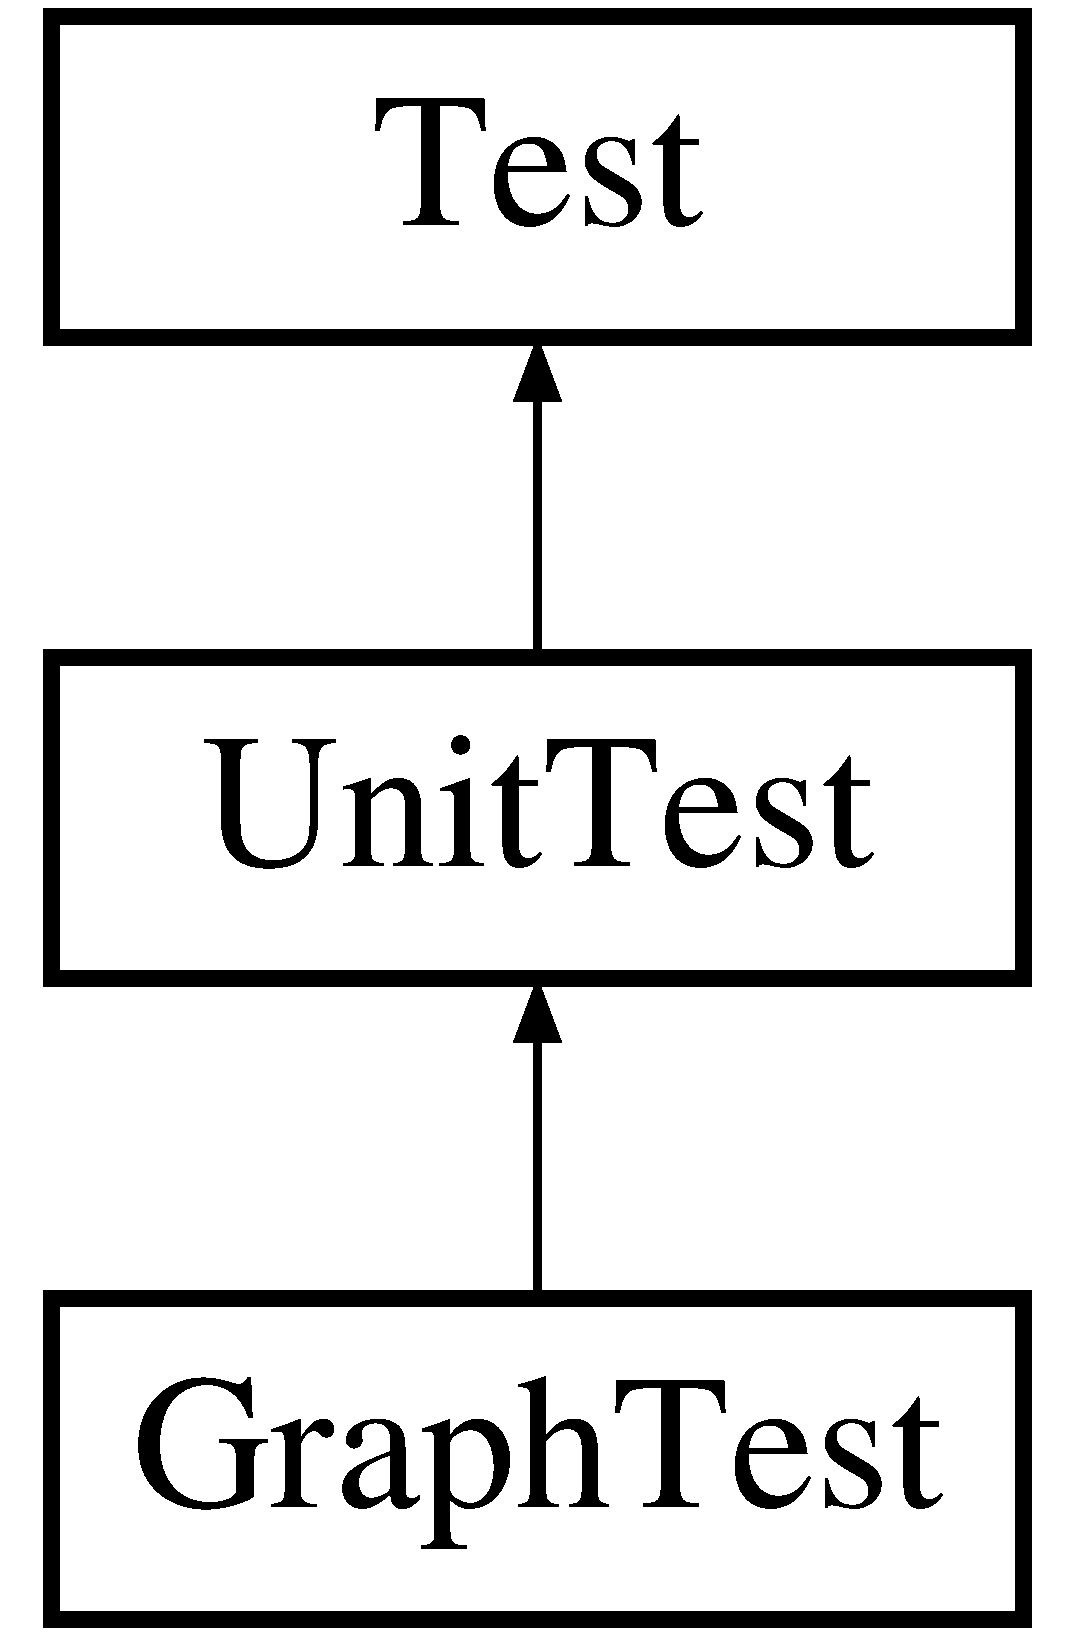
\includegraphics[height=3.000000cm]{classGraphTest}
\end{center}
\end{figure}
\subsection*{Public Member Functions}
\begin{DoxyCompactItemize}
\item 
\textbf{ Graph\+Test} (\textbf{ Test\+Suite} $\ast$s)
\item 
void \textbf{ setup} (void)
\item 
void \textbf{ cleanup} (void)
\item 
void \textbf{ test\+Vertices} (void)
\item 
void \textbf{ test\+Sample\+Values} (void)
\item 
void \textbf{ test\+Sample\+Occurences} (void)
\item 
void \textbf{ test\+Sample\+Value\+Adjacency\+Lists} (void)
\end{DoxyCompactItemize}
\subsection*{Private Attributes}
\begin{DoxyCompactItemize}
\item 
\textbf{ Cvr\+Stg\+File} $\ast$ \textbf{ f1}
\item 
\textbf{ Cvr\+Stg\+File} $\ast$ \textbf{ f2}
\item 
\textbf{ Cvr\+Stg\+File} $\ast$ \textbf{ f3}
\item 
\textbf{ Cvr\+Stg\+File} $\ast$ \textbf{ f4}
\item 
\textbf{ Cvr\+Stg\+File} $\ast$ \textbf{ f5}
\item 
\textbf{ Cvr\+Stg\+File} $\ast$ \textbf{ f6}
\item 
\textbf{ Cvr\+Stg\+File} $\ast$ \textbf{ f7}
\item 
\textbf{ Cvr\+Stg\+File} $\ast$ \textbf{ f8}
\item 
\textbf{ Cvr\+Stg\+File} $\ast$ \textbf{ f9}
\item 
\textbf{ Cvr\+Stg\+File} $\ast$ \textbf{ f10}
\item 
\textbf{ Cvr\+Stg\+File} $\ast$ \textbf{ f11}
\item 
\textbf{ Cvr\+Stg\+File} $\ast$ \textbf{ f12}
\item 
\textbf{ Cvr\+Stg\+File} $\ast$ \textbf{ f13}
\item 
\textbf{ Cvr\+Stg\+File} $\ast$ \textbf{ f14}
\item 
\textbf{ Cvr\+Stg\+File} $\ast$ \textbf{ f15}
\item 
\textbf{ Cvr\+Stg\+File} $\ast$ \textbf{ f\+\_\+f}
\item 
\textbf{ Bit\+String} $\ast$ \textbf{ bs1}
\item 
\textbf{ Bit\+String} $\ast$ \textbf{ bs2}
\item 
\textbf{ Bit\+String} $\ast$ \textbf{ bs3}
\item 
\textbf{ Bit\+String} $\ast$ \textbf{ bs4}
\item 
\textbf{ Bit\+String} $\ast$ \textbf{ bs5}
\item 
\textbf{ Bit\+String} $\ast$ \textbf{ bs6}
\item 
\textbf{ Bit\+String} $\ast$ \textbf{ bs7}
\item 
\textbf{ Bit\+String} $\ast$ \textbf{ bs8}
\item 
\textbf{ Bit\+String} $\ast$ \textbf{ bs9}
\item 
\textbf{ Bit\+String} $\ast$ \textbf{ bs10}
\item 
\textbf{ Bit\+String} $\ast$ \textbf{ bs11}
\item 
\textbf{ Bit\+String} $\ast$ \textbf{ bs12}
\item 
\textbf{ Bit\+String} $\ast$ \textbf{ bs13}
\item 
\textbf{ Bit\+String} $\ast$ \textbf{ bs14}
\item 
\textbf{ Bit\+String} $\ast$ \textbf{ bs15}
\item 
\textbf{ Bit\+String} $\ast$ \textbf{ bs\+\_\+f}
\item 
\textbf{ Selector} $\ast$ \textbf{ s1}
\item 
\textbf{ Selector} $\ast$ \textbf{ s2}
\item 
\textbf{ Selector} $\ast$ \textbf{ s3}
\item 
\textbf{ Selector} $\ast$ \textbf{ s4}
\item 
\textbf{ Selector} $\ast$ \textbf{ s5}
\item 
\textbf{ Selector} $\ast$ \textbf{ s6}
\item 
\textbf{ Selector} $\ast$ \textbf{ s7}
\item 
\textbf{ Selector} $\ast$ \textbf{ s8}
\item 
\textbf{ Selector} $\ast$ \textbf{ s9}
\item 
\textbf{ Selector} $\ast$ \textbf{ s10}
\item 
\textbf{ Selector} $\ast$ \textbf{ s11}
\item 
\textbf{ Selector} $\ast$ \textbf{ s12}
\item 
\textbf{ Selector} $\ast$ \textbf{ s13}
\item 
\textbf{ Selector} $\ast$ \textbf{ s14}
\item 
\textbf{ Selector} $\ast$ \textbf{ s15}
\item 
\textbf{ Selector} $\ast$ \textbf{ s\+\_\+f}
\item 
\textbf{ Graph} $\ast$ \textbf{ g1}
\item 
\textbf{ Graph} $\ast$ \textbf{ g2}
\item 
\textbf{ Graph} $\ast$ \textbf{ g3}
\item 
\textbf{ Graph} $\ast$ \textbf{ g4}
\item 
\textbf{ Graph} $\ast$ \textbf{ g5}
\item 
\textbf{ Graph} $\ast$ \textbf{ g6}
\item 
\textbf{ Graph} $\ast$ \textbf{ g7}
\item 
\textbf{ Graph} $\ast$ \textbf{ g8}
\item 
\textbf{ Graph} $\ast$ \textbf{ g9}
\item 
\textbf{ Graph} $\ast$ \textbf{ g10}
\item 
\textbf{ Graph} $\ast$ \textbf{ g11}
\item 
\textbf{ Graph} $\ast$ \textbf{ g12}
\item 
\textbf{ Graph} $\ast$ \textbf{ g13}
\item 
\textbf{ Graph} $\ast$ \textbf{ g14}
\item 
\textbf{ Graph} $\ast$ \textbf{ g15}
\item 
\textbf{ Graph} $\ast$ \textbf{ g\+\_\+f}
\item 
\textbf{ Globals} \textbf{ gl1}
\item 
\textbf{ Globals} \textbf{ gl2}
\item 
\textbf{ Globals} \textbf{ gl3}
\item 
\textbf{ Globals} \textbf{ gl4}
\item 
\textbf{ Globals} \textbf{ gl5}
\item 
\textbf{ Globals} \textbf{ gl6}
\item 
\textbf{ Globals} \textbf{ gl7}
\item 
\textbf{ Globals} \textbf{ gl8}
\item 
\textbf{ Globals} \textbf{ gl9}
\item 
\textbf{ Globals} \textbf{ gl10}
\item 
\textbf{ Globals} \textbf{ gl11}
\item 
\textbf{ Globals} \textbf{ gl12}
\item 
\textbf{ Globals} \textbf{ gl13}
\item 
\textbf{ Globals} \textbf{ gl14}
\item 
\textbf{ Globals} \textbf{ gl15}
\item 
\textbf{ Globals} \textbf{ gl\+\_\+f}
\end{DoxyCompactItemize}
\subsection*{Additional Inherited Members}


\subsection{Constructor \& Destructor Documentation}
\mbox{\label{classGraphTest_af9e7223112f0932029ef8120f9e0b0fd}} 
\index{Graph\+Test@{Graph\+Test}!Graph\+Test@{Graph\+Test}}
\index{Graph\+Test@{Graph\+Test}!Graph\+Test@{Graph\+Test}}
\subsubsection{Graph\+Test()}
{\footnotesize\ttfamily Graph\+Test\+::\+Graph\+Test (\begin{DoxyParamCaption}\item[{\textbf{ Test\+Suite} $\ast$}]{s }\end{DoxyParamCaption})}



\subsection{Member Function Documentation}
\mbox{\label{classGraphTest_a150987a43bbbdebc716152aaaa2c195d}} 
\index{Graph\+Test@{Graph\+Test}!cleanup@{cleanup}}
\index{cleanup@{cleanup}!Graph\+Test@{Graph\+Test}}
\subsubsection{cleanup()}
{\footnotesize\ttfamily void Graph\+Test\+::cleanup (\begin{DoxyParamCaption}\item[{void}]{ }\end{DoxyParamCaption})\hspace{0.3cm}{\ttfamily [virtual]}}

cleanup the unit test -\/ called after run 

Reimplemented from \textbf{ Unit\+Test} \doxyref{}{p.}{classUnitTest_adf77efe972ee4a766d94e3f7ddc193ad}.

\mbox{\label{classGraphTest_a5bfeaa205290aedf9c5ec8e6d011525e}} 
\index{Graph\+Test@{Graph\+Test}!setup@{setup}}
\index{setup@{setup}!Graph\+Test@{Graph\+Test}}
\subsubsection{setup()}
{\footnotesize\ttfamily void Graph\+Test\+::setup (\begin{DoxyParamCaption}\item[{void}]{ }\end{DoxyParamCaption})\hspace{0.3cm}{\ttfamily [virtual]}}

setup the unit test -\/ called before run

\doxyref{Unit\+Test\+::setup}{p.}{classUnitTest_ad73fdf9012b651047ea001d21f9d27ad} will (together with \doxyref{Unit\+Test\+::cleanup}{p.}{classUnitTest_adf77efe972ee4a766d94e3f7ddc193ad}) save and restore the object stored in Globs so they should be called from the corresponding functions in the derived object if the derived unit test manipulates the Globs object. 

Reimplemented from \textbf{ Unit\+Test} \doxyref{}{p.}{classUnitTest_ad73fdf9012b651047ea001d21f9d27ad}.

\mbox{\label{classGraphTest_ab14e7a0f74b25a9972639a5b314e0538}} 
\index{Graph\+Test@{Graph\+Test}!test\+Sample\+Occurences@{test\+Sample\+Occurences}}
\index{test\+Sample\+Occurences@{test\+Sample\+Occurences}!Graph\+Test@{Graph\+Test}}
\subsubsection{test\+Sample\+Occurences()}
{\footnotesize\ttfamily void Graph\+Test\+::test\+Sample\+Occurences (\begin{DoxyParamCaption}\item[{void}]{ }\end{DoxyParamCaption})}

\mbox{\label{classGraphTest_a0105abe8c81f1e4b4f89901affcb0cde}} 
\index{Graph\+Test@{Graph\+Test}!test\+Sample\+Value\+Adjacency\+Lists@{test\+Sample\+Value\+Adjacency\+Lists}}
\index{test\+Sample\+Value\+Adjacency\+Lists@{test\+Sample\+Value\+Adjacency\+Lists}!Graph\+Test@{Graph\+Test}}
\subsubsection{test\+Sample\+Value\+Adjacency\+Lists()}
{\footnotesize\ttfamily void Graph\+Test\+::test\+Sample\+Value\+Adjacency\+Lists (\begin{DoxyParamCaption}\item[{void}]{ }\end{DoxyParamCaption})}

\mbox{\label{classGraphTest_a73f9928b72cedc85b3d0e6ddbd98aa32}} 
\index{Graph\+Test@{Graph\+Test}!test\+Sample\+Values@{test\+Sample\+Values}}
\index{test\+Sample\+Values@{test\+Sample\+Values}!Graph\+Test@{Graph\+Test}}
\subsubsection{test\+Sample\+Values()}
{\footnotesize\ttfamily void Graph\+Test\+::test\+Sample\+Values (\begin{DoxyParamCaption}\item[{void}]{ }\end{DoxyParamCaption})}

\mbox{\label{classGraphTest_abf59a8a167ae7b34ed2c177a1b443e20}} 
\index{Graph\+Test@{Graph\+Test}!test\+Vertices@{test\+Vertices}}
\index{test\+Vertices@{test\+Vertices}!Graph\+Test@{Graph\+Test}}
\subsubsection{test\+Vertices()}
{\footnotesize\ttfamily void Graph\+Test\+::test\+Vertices (\begin{DoxyParamCaption}\item[{void}]{ }\end{DoxyParamCaption})}



\subsection{Member Data Documentation}
\mbox{\label{classGraphTest_abeea0d5a6e79074620125ccae2ef3f56}} 
\index{Graph\+Test@{Graph\+Test}!bs1@{bs1}}
\index{bs1@{bs1}!Graph\+Test@{Graph\+Test}}
\subsubsection{bs1}
{\footnotesize\ttfamily \textbf{ Bit\+String}$\ast$ Graph\+Test\+::bs1\hspace{0.3cm}{\ttfamily [private]}}

\mbox{\label{classGraphTest_a365fabbdefcdd94b07c2f6df8008b460}} 
\index{Graph\+Test@{Graph\+Test}!bs10@{bs10}}
\index{bs10@{bs10}!Graph\+Test@{Graph\+Test}}
\subsubsection{bs10}
{\footnotesize\ttfamily \textbf{ Bit\+String} $\ast$ Graph\+Test\+::bs10\hspace{0.3cm}{\ttfamily [private]}}

\mbox{\label{classGraphTest_a72cd11997a9e70ec6d68fb850c947c4d}} 
\index{Graph\+Test@{Graph\+Test}!bs11@{bs11}}
\index{bs11@{bs11}!Graph\+Test@{Graph\+Test}}
\subsubsection{bs11}
{\footnotesize\ttfamily \textbf{ Bit\+String} $\ast$ Graph\+Test\+::bs11\hspace{0.3cm}{\ttfamily [private]}}

\mbox{\label{classGraphTest_a2df2a8748e48b2fa738b89f79fa6e86d}} 
\index{Graph\+Test@{Graph\+Test}!bs12@{bs12}}
\index{bs12@{bs12}!Graph\+Test@{Graph\+Test}}
\subsubsection{bs12}
{\footnotesize\ttfamily \textbf{ Bit\+String} $\ast$ Graph\+Test\+::bs12\hspace{0.3cm}{\ttfamily [private]}}

\mbox{\label{classGraphTest_ad285ca0b83c494e2d03dd6505e43f2ee}} 
\index{Graph\+Test@{Graph\+Test}!bs13@{bs13}}
\index{bs13@{bs13}!Graph\+Test@{Graph\+Test}}
\subsubsection{bs13}
{\footnotesize\ttfamily \textbf{ Bit\+String} $\ast$ Graph\+Test\+::bs13\hspace{0.3cm}{\ttfamily [private]}}

\mbox{\label{classGraphTest_afdd2e8b312f7f9cd9f3a05b26bbe1b9b}} 
\index{Graph\+Test@{Graph\+Test}!bs14@{bs14}}
\index{bs14@{bs14}!Graph\+Test@{Graph\+Test}}
\subsubsection{bs14}
{\footnotesize\ttfamily \textbf{ Bit\+String} $\ast$ Graph\+Test\+::bs14\hspace{0.3cm}{\ttfamily [private]}}

\mbox{\label{classGraphTest_a4679c55fb445a0cf6a0209af5bd369a1}} 
\index{Graph\+Test@{Graph\+Test}!bs15@{bs15}}
\index{bs15@{bs15}!Graph\+Test@{Graph\+Test}}
\subsubsection{bs15}
{\footnotesize\ttfamily \textbf{ Bit\+String} $\ast$ Graph\+Test\+::bs15\hspace{0.3cm}{\ttfamily [private]}}

\mbox{\label{classGraphTest_a7f916264a5546bd69d73c0af62c99d96}} 
\index{Graph\+Test@{Graph\+Test}!bs2@{bs2}}
\index{bs2@{bs2}!Graph\+Test@{Graph\+Test}}
\subsubsection{bs2}
{\footnotesize\ttfamily \textbf{ Bit\+String} $\ast$ Graph\+Test\+::bs2\hspace{0.3cm}{\ttfamily [private]}}

\mbox{\label{classGraphTest_a90b820d304c2597e49e8e3f505ab3e7a}} 
\index{Graph\+Test@{Graph\+Test}!bs3@{bs3}}
\index{bs3@{bs3}!Graph\+Test@{Graph\+Test}}
\subsubsection{bs3}
{\footnotesize\ttfamily \textbf{ Bit\+String} $\ast$ Graph\+Test\+::bs3\hspace{0.3cm}{\ttfamily [private]}}

\mbox{\label{classGraphTest_aaadce8c48de1c65dc219ff7841f5784c}} 
\index{Graph\+Test@{Graph\+Test}!bs4@{bs4}}
\index{bs4@{bs4}!Graph\+Test@{Graph\+Test}}
\subsubsection{bs4}
{\footnotesize\ttfamily \textbf{ Bit\+String} $\ast$ Graph\+Test\+::bs4\hspace{0.3cm}{\ttfamily [private]}}

\mbox{\label{classGraphTest_a7d1111c4b26597860118428e1eac4aa5}} 
\index{Graph\+Test@{Graph\+Test}!bs5@{bs5}}
\index{bs5@{bs5}!Graph\+Test@{Graph\+Test}}
\subsubsection{bs5}
{\footnotesize\ttfamily \textbf{ Bit\+String} $\ast$ Graph\+Test\+::bs5\hspace{0.3cm}{\ttfamily [private]}}

\mbox{\label{classGraphTest_a6bd766ded4ceeaa89953ede40f0a0c47}} 
\index{Graph\+Test@{Graph\+Test}!bs6@{bs6}}
\index{bs6@{bs6}!Graph\+Test@{Graph\+Test}}
\subsubsection{bs6}
{\footnotesize\ttfamily \textbf{ Bit\+String} $\ast$ Graph\+Test\+::bs6\hspace{0.3cm}{\ttfamily [private]}}

\mbox{\label{classGraphTest_a301ec1976acf9a01784e745774f23fbb}} 
\index{Graph\+Test@{Graph\+Test}!bs7@{bs7}}
\index{bs7@{bs7}!Graph\+Test@{Graph\+Test}}
\subsubsection{bs7}
{\footnotesize\ttfamily \textbf{ Bit\+String} $\ast$ Graph\+Test\+::bs7\hspace{0.3cm}{\ttfamily [private]}}

\mbox{\label{classGraphTest_a04355cf1c4625349e76f39dcecda7a1b}} 
\index{Graph\+Test@{Graph\+Test}!bs8@{bs8}}
\index{bs8@{bs8}!Graph\+Test@{Graph\+Test}}
\subsubsection{bs8}
{\footnotesize\ttfamily \textbf{ Bit\+String} $\ast$ Graph\+Test\+::bs8\hspace{0.3cm}{\ttfamily [private]}}

\mbox{\label{classGraphTest_a0b5fe5bd1738ea52fdc751d9c0f3e163}} 
\index{Graph\+Test@{Graph\+Test}!bs9@{bs9}}
\index{bs9@{bs9}!Graph\+Test@{Graph\+Test}}
\subsubsection{bs9}
{\footnotesize\ttfamily \textbf{ Bit\+String} $\ast$ Graph\+Test\+::bs9\hspace{0.3cm}{\ttfamily [private]}}

\mbox{\label{classGraphTest_a2378982712dcadf9b37c19900335e404}} 
\index{Graph\+Test@{Graph\+Test}!bs\+\_\+f@{bs\+\_\+f}}
\index{bs\+\_\+f@{bs\+\_\+f}!Graph\+Test@{Graph\+Test}}
\subsubsection{bs\+\_\+f}
{\footnotesize\ttfamily \textbf{ Bit\+String} $\ast$ Graph\+Test\+::bs\+\_\+f\hspace{0.3cm}{\ttfamily [private]}}

\mbox{\label{classGraphTest_a913dfbbec347bf8a4492c8f448abe33b}} 
\index{Graph\+Test@{Graph\+Test}!f1@{f1}}
\index{f1@{f1}!Graph\+Test@{Graph\+Test}}
\subsubsection{f1}
{\footnotesize\ttfamily \textbf{ Cvr\+Stg\+File}$\ast$ Graph\+Test\+::f1\hspace{0.3cm}{\ttfamily [private]}}

\mbox{\label{classGraphTest_a0dcc2a7f75480eea555b6c7daa75ad87}} 
\index{Graph\+Test@{Graph\+Test}!f10@{f10}}
\index{f10@{f10}!Graph\+Test@{Graph\+Test}}
\subsubsection{f10}
{\footnotesize\ttfamily \textbf{ Cvr\+Stg\+File} $\ast$ Graph\+Test\+::f10\hspace{0.3cm}{\ttfamily [private]}}

\mbox{\label{classGraphTest_a653dcfe1b2fd5c1558cdd31d9db1b810}} 
\index{Graph\+Test@{Graph\+Test}!f11@{f11}}
\index{f11@{f11}!Graph\+Test@{Graph\+Test}}
\subsubsection{f11}
{\footnotesize\ttfamily \textbf{ Cvr\+Stg\+File} $\ast$ Graph\+Test\+::f11\hspace{0.3cm}{\ttfamily [private]}}

\mbox{\label{classGraphTest_aab9e495e6e14ddd2eee6d16ac4d28ff3}} 
\index{Graph\+Test@{Graph\+Test}!f12@{f12}}
\index{f12@{f12}!Graph\+Test@{Graph\+Test}}
\subsubsection{f12}
{\footnotesize\ttfamily \textbf{ Cvr\+Stg\+File} $\ast$ Graph\+Test\+::f12\hspace{0.3cm}{\ttfamily [private]}}

\mbox{\label{classGraphTest_a386b503a58956631659c4777758ede97}} 
\index{Graph\+Test@{Graph\+Test}!f13@{f13}}
\index{f13@{f13}!Graph\+Test@{Graph\+Test}}
\subsubsection{f13}
{\footnotesize\ttfamily \textbf{ Cvr\+Stg\+File} $\ast$ Graph\+Test\+::f13\hspace{0.3cm}{\ttfamily [private]}}

\mbox{\label{classGraphTest_a0ca113a67246f3255205d9ea56537d27}} 
\index{Graph\+Test@{Graph\+Test}!f14@{f14}}
\index{f14@{f14}!Graph\+Test@{Graph\+Test}}
\subsubsection{f14}
{\footnotesize\ttfamily \textbf{ Cvr\+Stg\+File} $\ast$ Graph\+Test\+::f14\hspace{0.3cm}{\ttfamily [private]}}

\mbox{\label{classGraphTest_a7d96b9611b3d37ea4d9e92e574d3bd62}} 
\index{Graph\+Test@{Graph\+Test}!f15@{f15}}
\index{f15@{f15}!Graph\+Test@{Graph\+Test}}
\subsubsection{f15}
{\footnotesize\ttfamily \textbf{ Cvr\+Stg\+File} $\ast$ Graph\+Test\+::f15\hspace{0.3cm}{\ttfamily [private]}}

\mbox{\label{classGraphTest_adca8f3dca77e5c1d0e06b74542186432}} 
\index{Graph\+Test@{Graph\+Test}!f2@{f2}}
\index{f2@{f2}!Graph\+Test@{Graph\+Test}}
\subsubsection{f2}
{\footnotesize\ttfamily \textbf{ Cvr\+Stg\+File} $\ast$ Graph\+Test\+::f2\hspace{0.3cm}{\ttfamily [private]}}

\mbox{\label{classGraphTest_ae85c1a68e5454a67b6c160713107d6df}} 
\index{Graph\+Test@{Graph\+Test}!f3@{f3}}
\index{f3@{f3}!Graph\+Test@{Graph\+Test}}
\subsubsection{f3}
{\footnotesize\ttfamily \textbf{ Cvr\+Stg\+File} $\ast$ Graph\+Test\+::f3\hspace{0.3cm}{\ttfamily [private]}}

\mbox{\label{classGraphTest_a6a87383d6ee1f6bd4001a84c7460b508}} 
\index{Graph\+Test@{Graph\+Test}!f4@{f4}}
\index{f4@{f4}!Graph\+Test@{Graph\+Test}}
\subsubsection{f4}
{\footnotesize\ttfamily \textbf{ Cvr\+Stg\+File} $\ast$ Graph\+Test\+::f4\hspace{0.3cm}{\ttfamily [private]}}

\mbox{\label{classGraphTest_a6a499086c8cbe82957aca03126650abc}} 
\index{Graph\+Test@{Graph\+Test}!f5@{f5}}
\index{f5@{f5}!Graph\+Test@{Graph\+Test}}
\subsubsection{f5}
{\footnotesize\ttfamily \textbf{ Cvr\+Stg\+File} $\ast$ Graph\+Test\+::f5\hspace{0.3cm}{\ttfamily [private]}}

\mbox{\label{classGraphTest_a79158cf83f5606835e34e8c1be808370}} 
\index{Graph\+Test@{Graph\+Test}!f6@{f6}}
\index{f6@{f6}!Graph\+Test@{Graph\+Test}}
\subsubsection{f6}
{\footnotesize\ttfamily \textbf{ Cvr\+Stg\+File} $\ast$ Graph\+Test\+::f6\hspace{0.3cm}{\ttfamily [private]}}

\mbox{\label{classGraphTest_a654540707e05847b0432b21883e761bc}} 
\index{Graph\+Test@{Graph\+Test}!f7@{f7}}
\index{f7@{f7}!Graph\+Test@{Graph\+Test}}
\subsubsection{f7}
{\footnotesize\ttfamily \textbf{ Cvr\+Stg\+File} $\ast$ Graph\+Test\+::f7\hspace{0.3cm}{\ttfamily [private]}}

\mbox{\label{classGraphTest_a3520c5180d78fe881ea0322d8ed135ae}} 
\index{Graph\+Test@{Graph\+Test}!f8@{f8}}
\index{f8@{f8}!Graph\+Test@{Graph\+Test}}
\subsubsection{f8}
{\footnotesize\ttfamily \textbf{ Cvr\+Stg\+File} $\ast$ Graph\+Test\+::f8\hspace{0.3cm}{\ttfamily [private]}}

\mbox{\label{classGraphTest_ae1c0142d6c99c3b6c97dcdb8c8372ed9}} 
\index{Graph\+Test@{Graph\+Test}!f9@{f9}}
\index{f9@{f9}!Graph\+Test@{Graph\+Test}}
\subsubsection{f9}
{\footnotesize\ttfamily \textbf{ Cvr\+Stg\+File} $\ast$ Graph\+Test\+::f9\hspace{0.3cm}{\ttfamily [private]}}

\mbox{\label{classGraphTest_af2ca79ff6dde64fabb061571328daeaa}} 
\index{Graph\+Test@{Graph\+Test}!f\+\_\+f@{f\+\_\+f}}
\index{f\+\_\+f@{f\+\_\+f}!Graph\+Test@{Graph\+Test}}
\subsubsection{f\+\_\+f}
{\footnotesize\ttfamily \textbf{ Cvr\+Stg\+File} $\ast$ Graph\+Test\+::f\+\_\+f\hspace{0.3cm}{\ttfamily [private]}}

\mbox{\label{classGraphTest_ab9cb4ede1aa33060509d3e7035a9b2a6}} 
\index{Graph\+Test@{Graph\+Test}!g1@{g1}}
\index{g1@{g1}!Graph\+Test@{Graph\+Test}}
\subsubsection{g1}
{\footnotesize\ttfamily \textbf{ Graph}$\ast$ Graph\+Test\+::g1\hspace{0.3cm}{\ttfamily [private]}}

\mbox{\label{classGraphTest_a250d0aa9e00baee79a5ea673576e884a}} 
\index{Graph\+Test@{Graph\+Test}!g10@{g10}}
\index{g10@{g10}!Graph\+Test@{Graph\+Test}}
\subsubsection{g10}
{\footnotesize\ttfamily \textbf{ Graph} $\ast$ Graph\+Test\+::g10\hspace{0.3cm}{\ttfamily [private]}}

\mbox{\label{classGraphTest_aee28711f63dbdeb0455d1b7fede3ea08}} 
\index{Graph\+Test@{Graph\+Test}!g11@{g11}}
\index{g11@{g11}!Graph\+Test@{Graph\+Test}}
\subsubsection{g11}
{\footnotesize\ttfamily \textbf{ Graph} $\ast$ Graph\+Test\+::g11\hspace{0.3cm}{\ttfamily [private]}}

\mbox{\label{classGraphTest_abeaaf662f91aa007563f093a885382db}} 
\index{Graph\+Test@{Graph\+Test}!g12@{g12}}
\index{g12@{g12}!Graph\+Test@{Graph\+Test}}
\subsubsection{g12}
{\footnotesize\ttfamily \textbf{ Graph} $\ast$ Graph\+Test\+::g12\hspace{0.3cm}{\ttfamily [private]}}

\mbox{\label{classGraphTest_a8a825cd8d0b8259f90755cc7bdd7be96}} 
\index{Graph\+Test@{Graph\+Test}!g13@{g13}}
\index{g13@{g13}!Graph\+Test@{Graph\+Test}}
\subsubsection{g13}
{\footnotesize\ttfamily \textbf{ Graph} $\ast$ Graph\+Test\+::g13\hspace{0.3cm}{\ttfamily [private]}}

\mbox{\label{classGraphTest_a1382881a95834c54f77daa8105c41fc0}} 
\index{Graph\+Test@{Graph\+Test}!g14@{g14}}
\index{g14@{g14}!Graph\+Test@{Graph\+Test}}
\subsubsection{g14}
{\footnotesize\ttfamily \textbf{ Graph} $\ast$ Graph\+Test\+::g14\hspace{0.3cm}{\ttfamily [private]}}

\mbox{\label{classGraphTest_ae47d893143db583e472bf770b7c4392f}} 
\index{Graph\+Test@{Graph\+Test}!g15@{g15}}
\index{g15@{g15}!Graph\+Test@{Graph\+Test}}
\subsubsection{g15}
{\footnotesize\ttfamily \textbf{ Graph} $\ast$ Graph\+Test\+::g15\hspace{0.3cm}{\ttfamily [private]}}

\mbox{\label{classGraphTest_a850cd937ac68fba6a5da69e013e34891}} 
\index{Graph\+Test@{Graph\+Test}!g2@{g2}}
\index{g2@{g2}!Graph\+Test@{Graph\+Test}}
\subsubsection{g2}
{\footnotesize\ttfamily \textbf{ Graph} $\ast$ Graph\+Test\+::g2\hspace{0.3cm}{\ttfamily [private]}}

\mbox{\label{classGraphTest_afd7f3baeb0b58a05b7a6e12fc85e00dc}} 
\index{Graph\+Test@{Graph\+Test}!g3@{g3}}
\index{g3@{g3}!Graph\+Test@{Graph\+Test}}
\subsubsection{g3}
{\footnotesize\ttfamily \textbf{ Graph} $\ast$ Graph\+Test\+::g3\hspace{0.3cm}{\ttfamily [private]}}

\mbox{\label{classGraphTest_ac788c87f4343cb7b66a18e5bb193de3e}} 
\index{Graph\+Test@{Graph\+Test}!g4@{g4}}
\index{g4@{g4}!Graph\+Test@{Graph\+Test}}
\subsubsection{g4}
{\footnotesize\ttfamily \textbf{ Graph} $\ast$ Graph\+Test\+::g4\hspace{0.3cm}{\ttfamily [private]}}

\mbox{\label{classGraphTest_a33aed29f97f718295763ad33d031c4f0}} 
\index{Graph\+Test@{Graph\+Test}!g5@{g5}}
\index{g5@{g5}!Graph\+Test@{Graph\+Test}}
\subsubsection{g5}
{\footnotesize\ttfamily \textbf{ Graph} $\ast$ Graph\+Test\+::g5\hspace{0.3cm}{\ttfamily [private]}}

\mbox{\label{classGraphTest_a548e3204a5d7d39b7022b1db0a2e4863}} 
\index{Graph\+Test@{Graph\+Test}!g6@{g6}}
\index{g6@{g6}!Graph\+Test@{Graph\+Test}}
\subsubsection{g6}
{\footnotesize\ttfamily \textbf{ Graph} $\ast$ Graph\+Test\+::g6\hspace{0.3cm}{\ttfamily [private]}}

\mbox{\label{classGraphTest_abf2159077e768aca536fa6f90874345d}} 
\index{Graph\+Test@{Graph\+Test}!g7@{g7}}
\index{g7@{g7}!Graph\+Test@{Graph\+Test}}
\subsubsection{g7}
{\footnotesize\ttfamily \textbf{ Graph} $\ast$ Graph\+Test\+::g7\hspace{0.3cm}{\ttfamily [private]}}

\mbox{\label{classGraphTest_aaa96ee53586c14ff33d4ef54ebb28533}} 
\index{Graph\+Test@{Graph\+Test}!g8@{g8}}
\index{g8@{g8}!Graph\+Test@{Graph\+Test}}
\subsubsection{g8}
{\footnotesize\ttfamily \textbf{ Graph} $\ast$ Graph\+Test\+::g8\hspace{0.3cm}{\ttfamily [private]}}

\mbox{\label{classGraphTest_a4abfa61dfad65a6aef2c806b01e521ec}} 
\index{Graph\+Test@{Graph\+Test}!g9@{g9}}
\index{g9@{g9}!Graph\+Test@{Graph\+Test}}
\subsubsection{g9}
{\footnotesize\ttfamily \textbf{ Graph} $\ast$ Graph\+Test\+::g9\hspace{0.3cm}{\ttfamily [private]}}

\mbox{\label{classGraphTest_a53c6b54d8ba8d18db5a398423ed7fd81}} 
\index{Graph\+Test@{Graph\+Test}!g\+\_\+f@{g\+\_\+f}}
\index{g\+\_\+f@{g\+\_\+f}!Graph\+Test@{Graph\+Test}}
\subsubsection{g\+\_\+f}
{\footnotesize\ttfamily \textbf{ Graph} $\ast$ Graph\+Test\+::g\+\_\+f\hspace{0.3cm}{\ttfamily [private]}}

\mbox{\label{classGraphTest_af332e086d934ce1d8eeff9849bb89145}} 
\index{Graph\+Test@{Graph\+Test}!gl1@{gl1}}
\index{gl1@{gl1}!Graph\+Test@{Graph\+Test}}
\subsubsection{gl1}
{\footnotesize\ttfamily \textbf{ Globals} Graph\+Test\+::gl1\hspace{0.3cm}{\ttfamily [private]}}

\mbox{\label{classGraphTest_ac412a7481451eb1fdbde841502903a7b}} 
\index{Graph\+Test@{Graph\+Test}!gl10@{gl10}}
\index{gl10@{gl10}!Graph\+Test@{Graph\+Test}}
\subsubsection{gl10}
{\footnotesize\ttfamily \textbf{ Globals} Graph\+Test\+::gl10\hspace{0.3cm}{\ttfamily [private]}}

\mbox{\label{classGraphTest_a426e7bf737c1eace92acc5cfda32f5a3}} 
\index{Graph\+Test@{Graph\+Test}!gl11@{gl11}}
\index{gl11@{gl11}!Graph\+Test@{Graph\+Test}}
\subsubsection{gl11}
{\footnotesize\ttfamily \textbf{ Globals} Graph\+Test\+::gl11\hspace{0.3cm}{\ttfamily [private]}}

\mbox{\label{classGraphTest_a124f4509d5734d983041bb5f50c94efb}} 
\index{Graph\+Test@{Graph\+Test}!gl12@{gl12}}
\index{gl12@{gl12}!Graph\+Test@{Graph\+Test}}
\subsubsection{gl12}
{\footnotesize\ttfamily \textbf{ Globals} Graph\+Test\+::gl12\hspace{0.3cm}{\ttfamily [private]}}

\mbox{\label{classGraphTest_a93e7ea2fc0731c4e9db1e79c27dcf632}} 
\index{Graph\+Test@{Graph\+Test}!gl13@{gl13}}
\index{gl13@{gl13}!Graph\+Test@{Graph\+Test}}
\subsubsection{gl13}
{\footnotesize\ttfamily \textbf{ Globals} Graph\+Test\+::gl13\hspace{0.3cm}{\ttfamily [private]}}

\mbox{\label{classGraphTest_a1164cd88e47df8d28ab7578e7f953b6d}} 
\index{Graph\+Test@{Graph\+Test}!gl14@{gl14}}
\index{gl14@{gl14}!Graph\+Test@{Graph\+Test}}
\subsubsection{gl14}
{\footnotesize\ttfamily \textbf{ Globals} Graph\+Test\+::gl14\hspace{0.3cm}{\ttfamily [private]}}

\mbox{\label{classGraphTest_a4317596fafe358e7c905d31398efb9f4}} 
\index{Graph\+Test@{Graph\+Test}!gl15@{gl15}}
\index{gl15@{gl15}!Graph\+Test@{Graph\+Test}}
\subsubsection{gl15}
{\footnotesize\ttfamily \textbf{ Globals} Graph\+Test\+::gl15\hspace{0.3cm}{\ttfamily [private]}}

\mbox{\label{classGraphTest_af3adb027f124083946769e29bbea3232}} 
\index{Graph\+Test@{Graph\+Test}!gl2@{gl2}}
\index{gl2@{gl2}!Graph\+Test@{Graph\+Test}}
\subsubsection{gl2}
{\footnotesize\ttfamily \textbf{ Globals} Graph\+Test\+::gl2\hspace{0.3cm}{\ttfamily [private]}}

\mbox{\label{classGraphTest_a61e6ac92054e2555868c3c8142d85fa3}} 
\index{Graph\+Test@{Graph\+Test}!gl3@{gl3}}
\index{gl3@{gl3}!Graph\+Test@{Graph\+Test}}
\subsubsection{gl3}
{\footnotesize\ttfamily \textbf{ Globals} Graph\+Test\+::gl3\hspace{0.3cm}{\ttfamily [private]}}

\mbox{\label{classGraphTest_a093465f7872b8c0ac79395923959f219}} 
\index{Graph\+Test@{Graph\+Test}!gl4@{gl4}}
\index{gl4@{gl4}!Graph\+Test@{Graph\+Test}}
\subsubsection{gl4}
{\footnotesize\ttfamily \textbf{ Globals} Graph\+Test\+::gl4\hspace{0.3cm}{\ttfamily [private]}}

\mbox{\label{classGraphTest_a6e770f804c84f8383138c945aaaef986}} 
\index{Graph\+Test@{Graph\+Test}!gl5@{gl5}}
\index{gl5@{gl5}!Graph\+Test@{Graph\+Test}}
\subsubsection{gl5}
{\footnotesize\ttfamily \textbf{ Globals} Graph\+Test\+::gl5\hspace{0.3cm}{\ttfamily [private]}}

\mbox{\label{classGraphTest_a01170b3f3e26bf7fede0515ba79a1a79}} 
\index{Graph\+Test@{Graph\+Test}!gl6@{gl6}}
\index{gl6@{gl6}!Graph\+Test@{Graph\+Test}}
\subsubsection{gl6}
{\footnotesize\ttfamily \textbf{ Globals} Graph\+Test\+::gl6\hspace{0.3cm}{\ttfamily [private]}}

\mbox{\label{classGraphTest_a91d2b3507dae18956c7e2c113c84dff4}} 
\index{Graph\+Test@{Graph\+Test}!gl7@{gl7}}
\index{gl7@{gl7}!Graph\+Test@{Graph\+Test}}
\subsubsection{gl7}
{\footnotesize\ttfamily \textbf{ Globals} Graph\+Test\+::gl7\hspace{0.3cm}{\ttfamily [private]}}

\mbox{\label{classGraphTest_a3726ed20ddcfd64fca9f20ab9d088c64}} 
\index{Graph\+Test@{Graph\+Test}!gl8@{gl8}}
\index{gl8@{gl8}!Graph\+Test@{Graph\+Test}}
\subsubsection{gl8}
{\footnotesize\ttfamily \textbf{ Globals} Graph\+Test\+::gl8\hspace{0.3cm}{\ttfamily [private]}}

\mbox{\label{classGraphTest_a00effe4454add56762d93c840dd61db3}} 
\index{Graph\+Test@{Graph\+Test}!gl9@{gl9}}
\index{gl9@{gl9}!Graph\+Test@{Graph\+Test}}
\subsubsection{gl9}
{\footnotesize\ttfamily \textbf{ Globals} Graph\+Test\+::gl9\hspace{0.3cm}{\ttfamily [private]}}

\mbox{\label{classGraphTest_aafc20b9bc13e5601de16edab9ee3a28d}} 
\index{Graph\+Test@{Graph\+Test}!gl\+\_\+f@{gl\+\_\+f}}
\index{gl\+\_\+f@{gl\+\_\+f}!Graph\+Test@{Graph\+Test}}
\subsubsection{gl\+\_\+f}
{\footnotesize\ttfamily \textbf{ Globals} Graph\+Test\+::gl\+\_\+f\hspace{0.3cm}{\ttfamily [private]}}

\mbox{\label{classGraphTest_a6a48cb1f7242a0abf7055cbc1b821ab9}} 
\index{Graph\+Test@{Graph\+Test}!s1@{s1}}
\index{s1@{s1}!Graph\+Test@{Graph\+Test}}
\subsubsection{s1}
{\footnotesize\ttfamily \textbf{ Selector}$\ast$ Graph\+Test\+::s1\hspace{0.3cm}{\ttfamily [private]}}

\mbox{\label{classGraphTest_afa5d53d08c3205ed917189bd62ca21ae}} 
\index{Graph\+Test@{Graph\+Test}!s10@{s10}}
\index{s10@{s10}!Graph\+Test@{Graph\+Test}}
\subsubsection{s10}
{\footnotesize\ttfamily \textbf{ Selector} $\ast$ Graph\+Test\+::s10\hspace{0.3cm}{\ttfamily [private]}}

\mbox{\label{classGraphTest_a14dc4e5c6974721acc02a1894ba3daf9}} 
\index{Graph\+Test@{Graph\+Test}!s11@{s11}}
\index{s11@{s11}!Graph\+Test@{Graph\+Test}}
\subsubsection{s11}
{\footnotesize\ttfamily \textbf{ Selector} $\ast$ Graph\+Test\+::s11\hspace{0.3cm}{\ttfamily [private]}}

\mbox{\label{classGraphTest_ab6adc105e4236275c06b8f13af2563c4}} 
\index{Graph\+Test@{Graph\+Test}!s12@{s12}}
\index{s12@{s12}!Graph\+Test@{Graph\+Test}}
\subsubsection{s12}
{\footnotesize\ttfamily \textbf{ Selector} $\ast$ Graph\+Test\+::s12\hspace{0.3cm}{\ttfamily [private]}}

\mbox{\label{classGraphTest_a2016379305b1c2ebc94ac703ad6be1a4}} 
\index{Graph\+Test@{Graph\+Test}!s13@{s13}}
\index{s13@{s13}!Graph\+Test@{Graph\+Test}}
\subsubsection{s13}
{\footnotesize\ttfamily \textbf{ Selector} $\ast$ Graph\+Test\+::s13\hspace{0.3cm}{\ttfamily [private]}}

\mbox{\label{classGraphTest_a996b670417cd878f0a69674dd86c3afd}} 
\index{Graph\+Test@{Graph\+Test}!s14@{s14}}
\index{s14@{s14}!Graph\+Test@{Graph\+Test}}
\subsubsection{s14}
{\footnotesize\ttfamily \textbf{ Selector} $\ast$ Graph\+Test\+::s14\hspace{0.3cm}{\ttfamily [private]}}

\mbox{\label{classGraphTest_a007b2564149f76d6fd7bf999265b4ee7}} 
\index{Graph\+Test@{Graph\+Test}!s15@{s15}}
\index{s15@{s15}!Graph\+Test@{Graph\+Test}}
\subsubsection{s15}
{\footnotesize\ttfamily \textbf{ Selector} $\ast$ Graph\+Test\+::s15\hspace{0.3cm}{\ttfamily [private]}}

\mbox{\label{classGraphTest_ac30aad76a742903474c58251bfe2f98a}} 
\index{Graph\+Test@{Graph\+Test}!s2@{s2}}
\index{s2@{s2}!Graph\+Test@{Graph\+Test}}
\subsubsection{s2}
{\footnotesize\ttfamily \textbf{ Selector} $\ast$ Graph\+Test\+::s2\hspace{0.3cm}{\ttfamily [private]}}

\mbox{\label{classGraphTest_a2a9d5ccec71a27369d39376621b617d3}} 
\index{Graph\+Test@{Graph\+Test}!s3@{s3}}
\index{s3@{s3}!Graph\+Test@{Graph\+Test}}
\subsubsection{s3}
{\footnotesize\ttfamily \textbf{ Selector} $\ast$ Graph\+Test\+::s3\hspace{0.3cm}{\ttfamily [private]}}

\mbox{\label{classGraphTest_a87ed1a9a1d11b16964d1c8f61edb9c05}} 
\index{Graph\+Test@{Graph\+Test}!s4@{s4}}
\index{s4@{s4}!Graph\+Test@{Graph\+Test}}
\subsubsection{s4}
{\footnotesize\ttfamily \textbf{ Selector} $\ast$ Graph\+Test\+::s4\hspace{0.3cm}{\ttfamily [private]}}

\mbox{\label{classGraphTest_ad21a4b974b445fd88d92a8815f42a705}} 
\index{Graph\+Test@{Graph\+Test}!s5@{s5}}
\index{s5@{s5}!Graph\+Test@{Graph\+Test}}
\subsubsection{s5}
{\footnotesize\ttfamily \textbf{ Selector} $\ast$ Graph\+Test\+::s5\hspace{0.3cm}{\ttfamily [private]}}

\mbox{\label{classGraphTest_a8a4a0152906a832366f04ae2d9e5725b}} 
\index{Graph\+Test@{Graph\+Test}!s6@{s6}}
\index{s6@{s6}!Graph\+Test@{Graph\+Test}}
\subsubsection{s6}
{\footnotesize\ttfamily \textbf{ Selector} $\ast$ Graph\+Test\+::s6\hspace{0.3cm}{\ttfamily [private]}}

\mbox{\label{classGraphTest_a21d258cf7a9e6a15e8f1d40e7b96ef97}} 
\index{Graph\+Test@{Graph\+Test}!s7@{s7}}
\index{s7@{s7}!Graph\+Test@{Graph\+Test}}
\subsubsection{s7}
{\footnotesize\ttfamily \textbf{ Selector} $\ast$ Graph\+Test\+::s7\hspace{0.3cm}{\ttfamily [private]}}

\mbox{\label{classGraphTest_a668c78151e48822689ddd46150d97e27}} 
\index{Graph\+Test@{Graph\+Test}!s8@{s8}}
\index{s8@{s8}!Graph\+Test@{Graph\+Test}}
\subsubsection{s8}
{\footnotesize\ttfamily \textbf{ Selector} $\ast$ Graph\+Test\+::s8\hspace{0.3cm}{\ttfamily [private]}}

\mbox{\label{classGraphTest_a8e004ecafc15c01b461dcdbe6c1f6e24}} 
\index{Graph\+Test@{Graph\+Test}!s9@{s9}}
\index{s9@{s9}!Graph\+Test@{Graph\+Test}}
\subsubsection{s9}
{\footnotesize\ttfamily \textbf{ Selector} $\ast$ Graph\+Test\+::s9\hspace{0.3cm}{\ttfamily [private]}}

\mbox{\label{classGraphTest_a5aad1e043031beaab30713f214e97c2a}} 
\index{Graph\+Test@{Graph\+Test}!s\+\_\+f@{s\+\_\+f}}
\index{s\+\_\+f@{s\+\_\+f}!Graph\+Test@{Graph\+Test}}
\subsubsection{s\+\_\+f}
{\footnotesize\ttfamily \textbf{ Selector} $\ast$ Graph\+Test\+::s\+\_\+f\hspace{0.3cm}{\ttfamily [private]}}



The documentation for this class was generated from the following files\+:\begin{DoxyCompactItemize}
\item 
\textbf{ Graph\+Test.\+h}\item 
\textbf{ Graph\+Test.\+cc}\end{DoxyCompactItemize}

\section{Jpeg\+File\+Test Class Reference}
\label{classJpegFileTest}\index{Jpeg\+File\+Test@{Jpeg\+File\+Test}}


{\ttfamily \#include $<$Jpeg\+File\+Test.\+h$>$}

Inheritance diagram for Jpeg\+File\+Test\+:\begin{figure}[H]
\begin{center}
\leavevmode
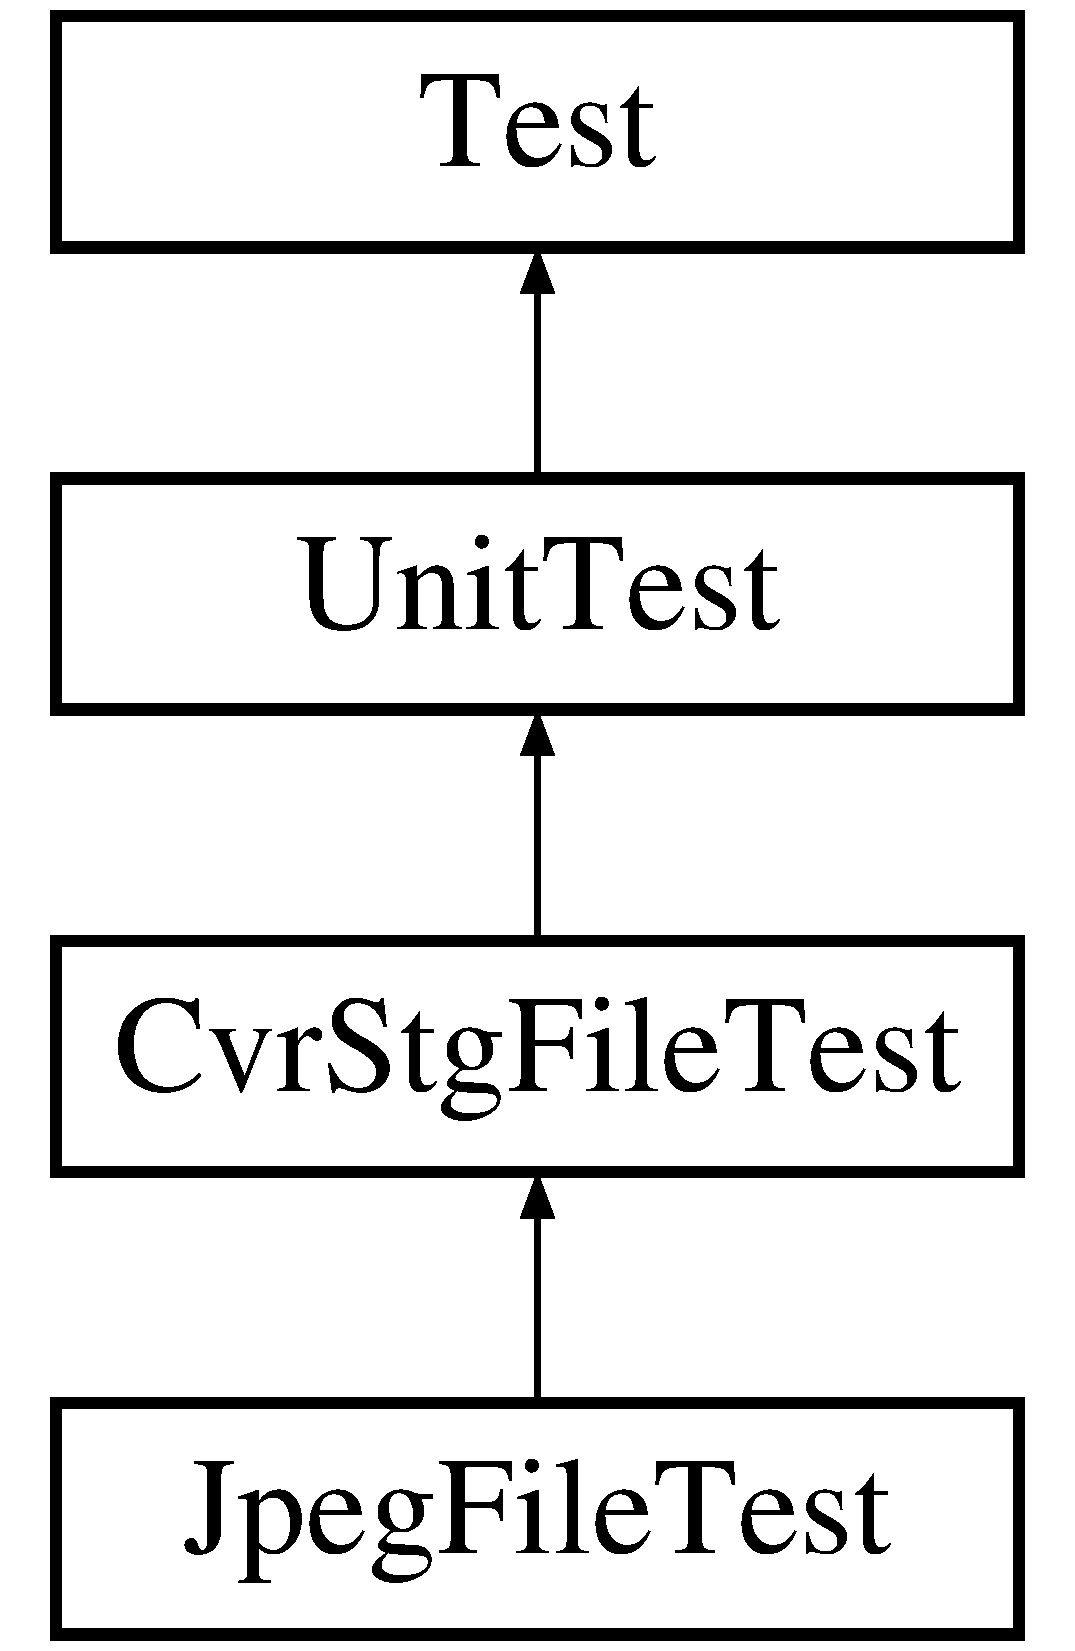
\includegraphics[height=4.000000cm]{classJpegFileTest}
\end{center}
\end{figure}
\subsection*{Public Member Functions}
\begin{DoxyCompactItemize}
\item 
\textbf{ Jpeg\+File\+Test} (\textbf{ Test\+Suite} $\ast$s)
\item 
void \textbf{ setup} (void)
\item 
void \textbf{ cleanup} (void)
\item 
void \textbf{ test\+Read\+Embed\+Extract} (void)
\item 
void \textbf{ test\+Read\+Embed\+Write\+Read\+Extract} (void)
\item 
void \textbf{ test\+Position} (void)
\item 
void \textbf{ test\+Read\+Extract\+Compare} (void)
\item 
void \textbf{ test\+Embedded\+Value} (void)
\end{DoxyCompactItemize}
\subsection*{Private Attributes}
\begin{DoxyCompactItemize}
\item 
\textbf{ Bit\+String} $\ast$ \textbf{ bs1}
\item 
\textbf{ Bit\+String} $\ast$ \textbf{ bs2}
\item 
\textbf{ Cvr\+Stg\+File} $\ast$ \textbf{ f1}
\item 
\textbf{ Cvr\+Stg\+File} $\ast$ \textbf{ f2}
\item 
\textbf{ Globals} \textbf{ gl1}
\item 
\textbf{ Globals} \textbf{ gl2}
\end{DoxyCompactItemize}
\subsection*{Additional Inherited Members}


\subsection{Constructor \& Destructor Documentation}
\mbox{\label{classJpegFileTest_a1808feac8e7b8bb3937015b80958f368}} 
\index{Jpeg\+File\+Test@{Jpeg\+File\+Test}!Jpeg\+File\+Test@{Jpeg\+File\+Test}}
\index{Jpeg\+File\+Test@{Jpeg\+File\+Test}!Jpeg\+File\+Test@{Jpeg\+File\+Test}}
\subsubsection{Jpeg\+File\+Test()}
{\footnotesize\ttfamily Jpeg\+File\+Test\+::\+Jpeg\+File\+Test (\begin{DoxyParamCaption}\item[{\textbf{ Test\+Suite} $\ast$}]{s }\end{DoxyParamCaption})}



\subsection{Member Function Documentation}
\mbox{\label{classJpegFileTest_a9d4011e0f9a932d1ad9af4869315bfc5}} 
\index{Jpeg\+File\+Test@{Jpeg\+File\+Test}!cleanup@{cleanup}}
\index{cleanup@{cleanup}!Jpeg\+File\+Test@{Jpeg\+File\+Test}}
\subsubsection{cleanup()}
{\footnotesize\ttfamily void Jpeg\+File\+Test\+::cleanup (\begin{DoxyParamCaption}\item[{void}]{ }\end{DoxyParamCaption})\hspace{0.3cm}{\ttfamily [virtual]}}

cleanup the unit test -\/ called after run 

Reimplemented from \textbf{ Unit\+Test} \doxyref{}{p.}{classUnitTest_adf77efe972ee4a766d94e3f7ddc193ad}.

\mbox{\label{classJpegFileTest_ab8796303fb34f7bbfd03a09bfef85b71}} 
\index{Jpeg\+File\+Test@{Jpeg\+File\+Test}!setup@{setup}}
\index{setup@{setup}!Jpeg\+File\+Test@{Jpeg\+File\+Test}}
\subsubsection{setup()}
{\footnotesize\ttfamily void Jpeg\+File\+Test\+::setup (\begin{DoxyParamCaption}\item[{void}]{ }\end{DoxyParamCaption})\hspace{0.3cm}{\ttfamily [virtual]}}

setup the unit test -\/ called before run

\doxyref{Unit\+Test\+::setup}{p.}{classUnitTest_ad73fdf9012b651047ea001d21f9d27ad} will (together with \doxyref{Unit\+Test\+::cleanup}{p.}{classUnitTest_adf77efe972ee4a766d94e3f7ddc193ad}) save and restore the object stored in Globs so they should be called from the corresponding functions in the derived object if the derived unit test manipulates the Globs object. 

Reimplemented from \textbf{ Unit\+Test} \doxyref{}{p.}{classUnitTest_ad73fdf9012b651047ea001d21f9d27ad}.

\mbox{\label{classJpegFileTest_adb1966b62d65d03280da4d16fecfd018}} 
\index{Jpeg\+File\+Test@{Jpeg\+File\+Test}!test\+Embedded\+Value@{test\+Embedded\+Value}}
\index{test\+Embedded\+Value@{test\+Embedded\+Value}!Jpeg\+File\+Test@{Jpeg\+File\+Test}}
\subsubsection{test\+Embedded\+Value()}
{\footnotesize\ttfamily void Jpeg\+File\+Test\+::test\+Embedded\+Value (\begin{DoxyParamCaption}\item[{void}]{ }\end{DoxyParamCaption})}

\mbox{\label{classJpegFileTest_a971cfd9d97810e9da2de352b986b7646}} 
\index{Jpeg\+File\+Test@{Jpeg\+File\+Test}!test\+Position@{test\+Position}}
\index{test\+Position@{test\+Position}!Jpeg\+File\+Test@{Jpeg\+File\+Test}}
\subsubsection{test\+Position()}
{\footnotesize\ttfamily void Jpeg\+File\+Test\+::test\+Position (\begin{DoxyParamCaption}\item[{void}]{ }\end{DoxyParamCaption})}

\mbox{\label{classJpegFileTest_a0ef20fae53ad23a422449e9224ffe843}} 
\index{Jpeg\+File\+Test@{Jpeg\+File\+Test}!test\+Read\+Embed\+Extract@{test\+Read\+Embed\+Extract}}
\index{test\+Read\+Embed\+Extract@{test\+Read\+Embed\+Extract}!Jpeg\+File\+Test@{Jpeg\+File\+Test}}
\subsubsection{test\+Read\+Embed\+Extract()}
{\footnotesize\ttfamily void Jpeg\+File\+Test\+::test\+Read\+Embed\+Extract (\begin{DoxyParamCaption}\item[{void}]{ }\end{DoxyParamCaption})}

\mbox{\label{classJpegFileTest_a251f4a3d0b2c58bdeb7552618cf675b0}} 
\index{Jpeg\+File\+Test@{Jpeg\+File\+Test}!test\+Read\+Embed\+Write\+Read\+Extract@{test\+Read\+Embed\+Write\+Read\+Extract}}
\index{test\+Read\+Embed\+Write\+Read\+Extract@{test\+Read\+Embed\+Write\+Read\+Extract}!Jpeg\+File\+Test@{Jpeg\+File\+Test}}
\subsubsection{test\+Read\+Embed\+Write\+Read\+Extract()}
{\footnotesize\ttfamily void Jpeg\+File\+Test\+::test\+Read\+Embed\+Write\+Read\+Extract (\begin{DoxyParamCaption}\item[{void}]{ }\end{DoxyParamCaption})}

\mbox{\label{classJpegFileTest_a49f1e1f0899346a024a50821c301fed7}} 
\index{Jpeg\+File\+Test@{Jpeg\+File\+Test}!test\+Read\+Extract\+Compare@{test\+Read\+Extract\+Compare}}
\index{test\+Read\+Extract\+Compare@{test\+Read\+Extract\+Compare}!Jpeg\+File\+Test@{Jpeg\+File\+Test}}
\subsubsection{test\+Read\+Extract\+Compare()}
{\footnotesize\ttfamily void Jpeg\+File\+Test\+::test\+Read\+Extract\+Compare (\begin{DoxyParamCaption}\item[{void}]{ }\end{DoxyParamCaption})}



\subsection{Member Data Documentation}
\mbox{\label{classJpegFileTest_a66421aace16f4b37097da94fabead924}} 
\index{Jpeg\+File\+Test@{Jpeg\+File\+Test}!bs1@{bs1}}
\index{bs1@{bs1}!Jpeg\+File\+Test@{Jpeg\+File\+Test}}
\subsubsection{bs1}
{\footnotesize\ttfamily \textbf{ Bit\+String}$\ast$ Jpeg\+File\+Test\+::bs1\hspace{0.3cm}{\ttfamily [private]}}

\mbox{\label{classJpegFileTest_a1d28b01674cac8e500d4055db243938a}} 
\index{Jpeg\+File\+Test@{Jpeg\+File\+Test}!bs2@{bs2}}
\index{bs2@{bs2}!Jpeg\+File\+Test@{Jpeg\+File\+Test}}
\subsubsection{bs2}
{\footnotesize\ttfamily \textbf{ Bit\+String} $\ast$ Jpeg\+File\+Test\+::bs2\hspace{0.3cm}{\ttfamily [private]}}

\mbox{\label{classJpegFileTest_af8a0c07ffc925e49f4d3e5557f64ac86}} 
\index{Jpeg\+File\+Test@{Jpeg\+File\+Test}!f1@{f1}}
\index{f1@{f1}!Jpeg\+File\+Test@{Jpeg\+File\+Test}}
\subsubsection{f1}
{\footnotesize\ttfamily \textbf{ Cvr\+Stg\+File}$\ast$ Jpeg\+File\+Test\+::f1\hspace{0.3cm}{\ttfamily [private]}}

\mbox{\label{classJpegFileTest_a88585db1f2a9192671a4bbbcdc5501ce}} 
\index{Jpeg\+File\+Test@{Jpeg\+File\+Test}!f2@{f2}}
\index{f2@{f2}!Jpeg\+File\+Test@{Jpeg\+File\+Test}}
\subsubsection{f2}
{\footnotesize\ttfamily \textbf{ Cvr\+Stg\+File} $\ast$ Jpeg\+File\+Test\+::f2\hspace{0.3cm}{\ttfamily [private]}}

\mbox{\label{classJpegFileTest_a62e959f10df3d26596a7d9546d92e707}} 
\index{Jpeg\+File\+Test@{Jpeg\+File\+Test}!gl1@{gl1}}
\index{gl1@{gl1}!Jpeg\+File\+Test@{Jpeg\+File\+Test}}
\subsubsection{gl1}
{\footnotesize\ttfamily \textbf{ Globals} Jpeg\+File\+Test\+::gl1\hspace{0.3cm}{\ttfamily [private]}}

\mbox{\label{classJpegFileTest_a7c36d3ac80d19c24c6f795397bbe5729}} 
\index{Jpeg\+File\+Test@{Jpeg\+File\+Test}!gl2@{gl2}}
\index{gl2@{gl2}!Jpeg\+File\+Test@{Jpeg\+File\+Test}}
\subsubsection{gl2}
{\footnotesize\ttfamily \textbf{ Globals} Jpeg\+File\+Test\+::gl2\hspace{0.3cm}{\ttfamily [private]}}



The documentation for this class was generated from the following files\+:\begin{DoxyCompactItemize}
\item 
\textbf{ Jpeg\+File\+Test.\+h}\item 
\textbf{ Jpeg\+File\+Test.\+cc}\end{DoxyCompactItemize}

\section{Jpeg\+Sample\+Value Class Reference}
\label{classJpegSampleValue}\index{Jpeg\+Sample\+Value@{Jpeg\+Sample\+Value}}


{\ttfamily \#include $<$Jpeg\+Sample\+Value.\+h$>$}

Inheritance diagram for Jpeg\+Sample\+Value\+:\begin{figure}[H]
\begin{center}
\leavevmode
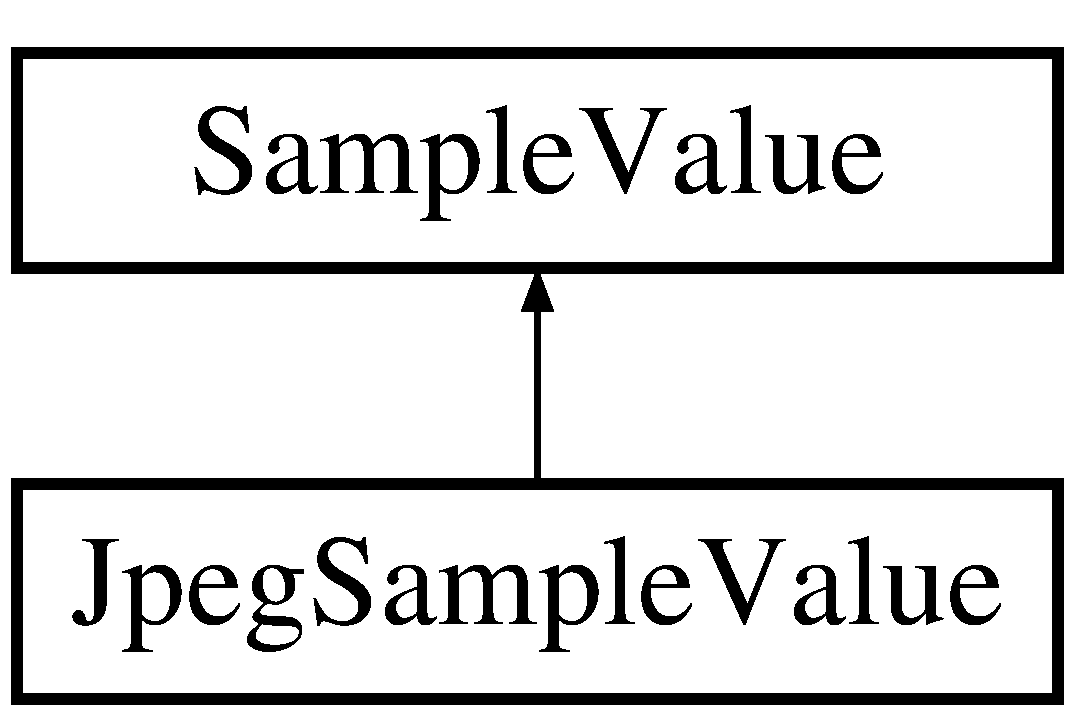
\includegraphics[height=2.000000cm]{classJpegSampleValue}
\end{center}
\end{figure}
\subsection*{Public Member Functions}
\begin{DoxyCompactItemize}
\item 
\textbf{ Jpeg\+Sample\+Value} (int c)
\item 
\textbf{ Sample\+Value} $\ast$ \textbf{ get\+Nearest\+Target\+Sample\+Value} (\textbf{ Emb\+Value} t) const
\item 
\textbf{ U\+W\+O\+R\+D32} \textbf{ calc\+Distance} (const \textbf{ Sample\+Value} $\ast$s) const
\item 
std\+::string \textbf{ get\+Name} (void) const
\item 
\textbf{ S\+W\+O\+R\+D16} \textbf{ get\+Dct\+Coeff} (void) const
\end{DoxyCompactItemize}
\subsection*{Static Public Member Functions}
\begin{DoxyCompactItemize}
\item 
static \textbf{ Emb\+Value} \textbf{ calc\+E\+Value} (\textbf{ S\+W\+O\+R\+D16} dctc)
\end{DoxyCompactItemize}
\subsection*{Private Attributes}
\begin{DoxyCompactItemize}
\item 
\textbf{ S\+W\+O\+R\+D16} \textbf{ Dct\+Coeff}
\end{DoxyCompactItemize}
\subsection*{Additional Inherited Members}


\subsection{Constructor \& Destructor Documentation}
\mbox{\label{classJpegSampleValue_a56c663648ba670a7e9dfe75326940227}} 
\index{Jpeg\+Sample\+Value@{Jpeg\+Sample\+Value}!Jpeg\+Sample\+Value@{Jpeg\+Sample\+Value}}
\index{Jpeg\+Sample\+Value@{Jpeg\+Sample\+Value}!Jpeg\+Sample\+Value@{Jpeg\+Sample\+Value}}
\subsubsection{Jpeg\+Sample\+Value()}
{\footnotesize\ttfamily Jpeg\+Sample\+Value\+::\+Jpeg\+Sample\+Value (\begin{DoxyParamCaption}\item[{int}]{c }\end{DoxyParamCaption})}



\subsection{Member Function Documentation}
\mbox{\label{classJpegSampleValue_a94973d445cd7b4d40e767f533f38164b}} 
\index{Jpeg\+Sample\+Value@{Jpeg\+Sample\+Value}!calc\+Distance@{calc\+Distance}}
\index{calc\+Distance@{calc\+Distance}!Jpeg\+Sample\+Value@{Jpeg\+Sample\+Value}}
\subsubsection{calc\+Distance()}
{\footnotesize\ttfamily \textbf{ U\+W\+O\+R\+D32} Jpeg\+Sample\+Value\+::calc\+Distance (\begin{DoxyParamCaption}\item[{const \textbf{ Sample\+Value} $\ast$}]{s }\end{DoxyParamCaption}) const\hspace{0.3cm}{\ttfamily [virtual]}}

calculate the distance between the sample value s and this sample value 
\begin{DoxyParams}{Parameters}
{\em s} & a sample value of the same type as this \\
\hline
\end{DoxyParams}
\begin{DoxyReturn}{Returns}
the distance 
\end{DoxyReturn}


Implements \textbf{ Sample\+Value} \doxyref{}{p.}{classSampleValue_aa7e5d9b69203f6f6edf97c79319232dd}.

\mbox{\label{classJpegSampleValue_a06fbe97eb12bf1b5c5ad6f995973f2d2}} 
\index{Jpeg\+Sample\+Value@{Jpeg\+Sample\+Value}!calc\+E\+Value@{calc\+E\+Value}}
\index{calc\+E\+Value@{calc\+E\+Value}!Jpeg\+Sample\+Value@{Jpeg\+Sample\+Value}}
\subsubsection{calc\+E\+Value()}
{\footnotesize\ttfamily static \textbf{ Emb\+Value} Jpeg\+Sample\+Value\+::calc\+E\+Value (\begin{DoxyParamCaption}\item[{\textbf{ S\+W\+O\+R\+D16}}]{dctc }\end{DoxyParamCaption})\hspace{0.3cm}{\ttfamily [inline]}, {\ttfamily [static]}}

\mbox{\label{classJpegSampleValue_a5f6ada9afca73df726a206c3165526ae}} 
\index{Jpeg\+Sample\+Value@{Jpeg\+Sample\+Value}!get\+Dct\+Coeff@{get\+Dct\+Coeff}}
\index{get\+Dct\+Coeff@{get\+Dct\+Coeff}!Jpeg\+Sample\+Value@{Jpeg\+Sample\+Value}}
\subsubsection{get\+Dct\+Coeff()}
{\footnotesize\ttfamily \textbf{ S\+W\+O\+R\+D16} Jpeg\+Sample\+Value\+::get\+Dct\+Coeff (\begin{DoxyParamCaption}\item[{void}]{ }\end{DoxyParamCaption}) const\hspace{0.3cm}{\ttfamily [inline]}}

\mbox{\label{classJpegSampleValue_a8d030038b36fff2478ed0eaf212bc73f}} 
\index{Jpeg\+Sample\+Value@{Jpeg\+Sample\+Value}!get\+Name@{get\+Name}}
\index{get\+Name@{get\+Name}!Jpeg\+Sample\+Value@{Jpeg\+Sample\+Value}}
\subsubsection{get\+Name()}
{\footnotesize\ttfamily std\+::string Jpeg\+Sample\+Value\+::get\+Name (\begin{DoxyParamCaption}\item[{void}]{ }\end{DoxyParamCaption}) const\hspace{0.3cm}{\ttfamily [virtual]}}

return a short name uniquely identifying this sample value 

Implements \textbf{ Sample\+Value} \doxyref{}{p.}{classSampleValue_aeaf5c46ec6d023840e9773604b20d25c}.

\mbox{\label{classJpegSampleValue_afcd941c26dea216970e6da945cb78511}} 
\index{Jpeg\+Sample\+Value@{Jpeg\+Sample\+Value}!get\+Nearest\+Target\+Sample\+Value@{get\+Nearest\+Target\+Sample\+Value}}
\index{get\+Nearest\+Target\+Sample\+Value@{get\+Nearest\+Target\+Sample\+Value}!Jpeg\+Sample\+Value@{Jpeg\+Sample\+Value}}
\subsubsection{get\+Nearest\+Target\+Sample\+Value()}
{\footnotesize\ttfamily \textbf{ Sample\+Value} $\ast$ Jpeg\+Sample\+Value\+::get\+Nearest\+Target\+Sample\+Value (\begin{DoxyParamCaption}\item[{\textbf{ Emb\+Value}}]{t }\end{DoxyParamCaption}) const\hspace{0.3cm}{\ttfamily [virtual]}}

get the nearest (with the least distance to this sample value) sample value whose embedded value equals the specified target 
\begin{DoxyParams}{Parameters}
{\em t} & the target embedded value\\
\hline
\end{DoxyParams}
If two or more target sample values have equal distance each of them should be returned with equal probability.

The returned \doxyref{Sample\+Value}{p.}{classSampleValue} object should be deleted by the callser. 

Implements \textbf{ Sample\+Value} \doxyref{}{p.}{classSampleValue_aeca3fc1fd34c09d2244706b010935c2c}.



\subsection{Member Data Documentation}
\mbox{\label{classJpegSampleValue_ad51e8f0375dbb30b66ff3f83b4665a08}} 
\index{Jpeg\+Sample\+Value@{Jpeg\+Sample\+Value}!Dct\+Coeff@{Dct\+Coeff}}
\index{Dct\+Coeff@{Dct\+Coeff}!Jpeg\+Sample\+Value@{Jpeg\+Sample\+Value}}
\subsubsection{Dct\+Coeff}
{\footnotesize\ttfamily \textbf{ S\+W\+O\+R\+D16} Jpeg\+Sample\+Value\+::\+Dct\+Coeff\hspace{0.3cm}{\ttfamily [private]}}



The documentation for this class was generated from the following files\+:\begin{DoxyCompactItemize}
\item 
\textbf{ Jpeg\+Sample\+Value.\+h}\item 
\textbf{ Jpeg\+Sample\+Value.\+cc}\end{DoxyCompactItemize}

\section{Jpeg\+Sample\+Value\+Test Class Reference}
\label{classJpegSampleValueTest}\index{Jpeg\+Sample\+Value\+Test@{Jpeg\+Sample\+Value\+Test}}


{\ttfamily \#include $<$Jpeg\+Sample\+Value\+Test.\+h$>$}

Inheritance diagram for Jpeg\+Sample\+Value\+Test\+:\begin{figure}[H]
\begin{center}
\leavevmode
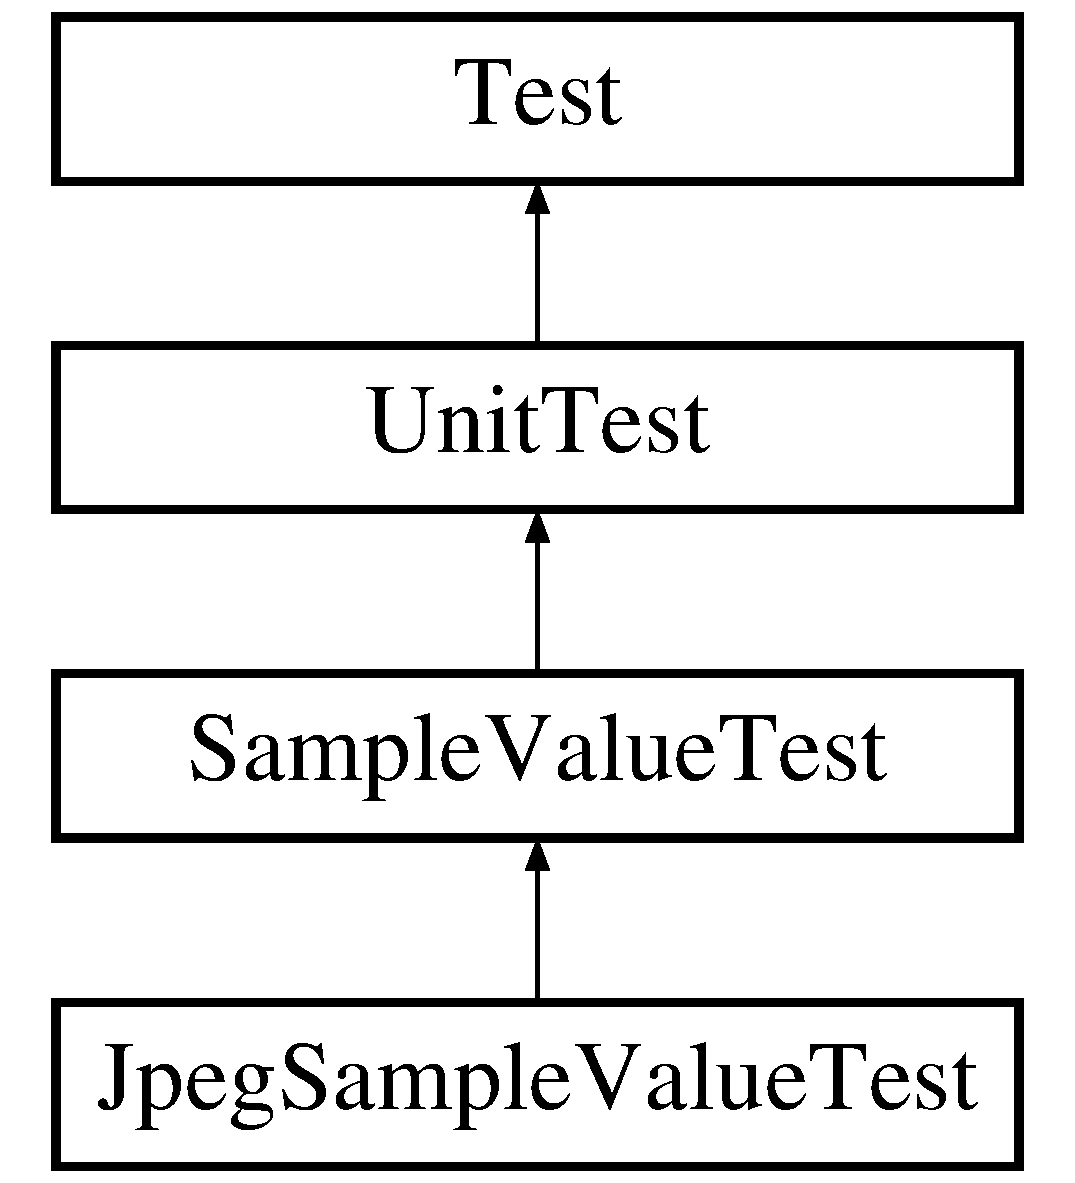
\includegraphics[height=4.000000cm]{classJpegSampleValueTest}
\end{center}
\end{figure}
\subsection*{Public Member Functions}
\begin{DoxyCompactItemize}
\item 
\textbf{ Jpeg\+Sample\+Value\+Test} (\textbf{ Test\+Suite} $\ast$s)
\item 
void \textbf{ setup} (void)
\item 
void \textbf{ cleanup} (void)
\item 
void \textbf{ test\+Distance} (void)
\item 
void \textbf{ test\+Is\+Neighbour} (void)
\end{DoxyCompactItemize}
\subsection*{Private Attributes}
\begin{DoxyCompactItemize}
\item 
\textbf{ Cvr\+Stg\+File} $\ast$ \textbf{ f1}
\item 
\textbf{ Jpeg\+Sample\+Value} $\ast$ \textbf{ sv\+\_\+m1}
\item 
\textbf{ Jpeg\+Sample\+Value} $\ast$ \textbf{ sv\+\_\+0}
\item 
\textbf{ Jpeg\+Sample\+Value} $\ast$ \textbf{ sv\+\_\+1}
\item 
\textbf{ Globals} \textbf{ gl1}
\end{DoxyCompactItemize}
\subsection*{Additional Inherited Members}


\subsection{Constructor \& Destructor Documentation}
\mbox{\label{classJpegSampleValueTest_a950be13638e9ecd4ef9bbd10d82c42f0}} 
\index{Jpeg\+Sample\+Value\+Test@{Jpeg\+Sample\+Value\+Test}!Jpeg\+Sample\+Value\+Test@{Jpeg\+Sample\+Value\+Test}}
\index{Jpeg\+Sample\+Value\+Test@{Jpeg\+Sample\+Value\+Test}!Jpeg\+Sample\+Value\+Test@{Jpeg\+Sample\+Value\+Test}}
\subsubsection{Jpeg\+Sample\+Value\+Test()}
{\footnotesize\ttfamily Jpeg\+Sample\+Value\+Test\+::\+Jpeg\+Sample\+Value\+Test (\begin{DoxyParamCaption}\item[{\textbf{ Test\+Suite} $\ast$}]{s }\end{DoxyParamCaption})}



\subsection{Member Function Documentation}
\mbox{\label{classJpegSampleValueTest_a98099c2d4c7bbd0bb78c5310603b2b98}} 
\index{Jpeg\+Sample\+Value\+Test@{Jpeg\+Sample\+Value\+Test}!cleanup@{cleanup}}
\index{cleanup@{cleanup}!Jpeg\+Sample\+Value\+Test@{Jpeg\+Sample\+Value\+Test}}
\subsubsection{cleanup()}
{\footnotesize\ttfamily void Jpeg\+Sample\+Value\+Test\+::cleanup (\begin{DoxyParamCaption}\item[{void}]{ }\end{DoxyParamCaption})\hspace{0.3cm}{\ttfamily [virtual]}}

cleanup the unit test -\/ called after run 

Reimplemented from \textbf{ Unit\+Test} \doxyref{}{p.}{classUnitTest_adf77efe972ee4a766d94e3f7ddc193ad}.

\mbox{\label{classJpegSampleValueTest_ab0bad2a2543a8cc19db4aced314a1f03}} 
\index{Jpeg\+Sample\+Value\+Test@{Jpeg\+Sample\+Value\+Test}!setup@{setup}}
\index{setup@{setup}!Jpeg\+Sample\+Value\+Test@{Jpeg\+Sample\+Value\+Test}}
\subsubsection{setup()}
{\footnotesize\ttfamily void Jpeg\+Sample\+Value\+Test\+::setup (\begin{DoxyParamCaption}\item[{void}]{ }\end{DoxyParamCaption})\hspace{0.3cm}{\ttfamily [virtual]}}

setup the unit test -\/ called before run

\doxyref{Unit\+Test\+::setup}{p.}{classUnitTest_ad73fdf9012b651047ea001d21f9d27ad} will (together with \doxyref{Unit\+Test\+::cleanup}{p.}{classUnitTest_adf77efe972ee4a766d94e3f7ddc193ad}) save and restore the object stored in Globs so they should be called from the corresponding functions in the derived object if the derived unit test manipulates the Globs object. 

Reimplemented from \textbf{ Unit\+Test} \doxyref{}{p.}{classUnitTest_ad73fdf9012b651047ea001d21f9d27ad}.

\mbox{\label{classJpegSampleValueTest_a9cd38f9ed8c9e595209022f5b9d5b7b9}} 
\index{Jpeg\+Sample\+Value\+Test@{Jpeg\+Sample\+Value\+Test}!test\+Distance@{test\+Distance}}
\index{test\+Distance@{test\+Distance}!Jpeg\+Sample\+Value\+Test@{Jpeg\+Sample\+Value\+Test}}
\subsubsection{test\+Distance()}
{\footnotesize\ttfamily void Jpeg\+Sample\+Value\+Test\+::test\+Distance (\begin{DoxyParamCaption}\item[{void}]{ }\end{DoxyParamCaption})}

\mbox{\label{classJpegSampleValueTest_a9ad2caf62f6decbbaa69e66594717d58}} 
\index{Jpeg\+Sample\+Value\+Test@{Jpeg\+Sample\+Value\+Test}!test\+Is\+Neighbour@{test\+Is\+Neighbour}}
\index{test\+Is\+Neighbour@{test\+Is\+Neighbour}!Jpeg\+Sample\+Value\+Test@{Jpeg\+Sample\+Value\+Test}}
\subsubsection{test\+Is\+Neighbour()}
{\footnotesize\ttfamily void Jpeg\+Sample\+Value\+Test\+::test\+Is\+Neighbour (\begin{DoxyParamCaption}\item[{void}]{ }\end{DoxyParamCaption})}



\subsection{Member Data Documentation}
\mbox{\label{classJpegSampleValueTest_af040347769054ee0ba5b2007bb068481}} 
\index{Jpeg\+Sample\+Value\+Test@{Jpeg\+Sample\+Value\+Test}!f1@{f1}}
\index{f1@{f1}!Jpeg\+Sample\+Value\+Test@{Jpeg\+Sample\+Value\+Test}}
\subsubsection{f1}
{\footnotesize\ttfamily \textbf{ Cvr\+Stg\+File}$\ast$ Jpeg\+Sample\+Value\+Test\+::f1\hspace{0.3cm}{\ttfamily [private]}}

\mbox{\label{classJpegSampleValueTest_a27312cd3baca326ea1d74f8c6d32cfc0}} 
\index{Jpeg\+Sample\+Value\+Test@{Jpeg\+Sample\+Value\+Test}!gl1@{gl1}}
\index{gl1@{gl1}!Jpeg\+Sample\+Value\+Test@{Jpeg\+Sample\+Value\+Test}}
\subsubsection{gl1}
{\footnotesize\ttfamily \textbf{ Globals} Jpeg\+Sample\+Value\+Test\+::gl1\hspace{0.3cm}{\ttfamily [private]}}

\mbox{\label{classJpegSampleValueTest_a52cec03bb4a6145a32835d206326e866}} 
\index{Jpeg\+Sample\+Value\+Test@{Jpeg\+Sample\+Value\+Test}!sv\+\_\+0@{sv\+\_\+0}}
\index{sv\+\_\+0@{sv\+\_\+0}!Jpeg\+Sample\+Value\+Test@{Jpeg\+Sample\+Value\+Test}}
\subsubsection{sv\+\_\+0}
{\footnotesize\ttfamily \textbf{ Jpeg\+Sample\+Value} $\ast$ Jpeg\+Sample\+Value\+Test\+::sv\+\_\+0\hspace{0.3cm}{\ttfamily [private]}}

\mbox{\label{classJpegSampleValueTest_a0e17ed06276b22c89182743d3e219b6e}} 
\index{Jpeg\+Sample\+Value\+Test@{Jpeg\+Sample\+Value\+Test}!sv\+\_\+1@{sv\+\_\+1}}
\index{sv\+\_\+1@{sv\+\_\+1}!Jpeg\+Sample\+Value\+Test@{Jpeg\+Sample\+Value\+Test}}
\subsubsection{sv\+\_\+1}
{\footnotesize\ttfamily \textbf{ Jpeg\+Sample\+Value} $\ast$ Jpeg\+Sample\+Value\+Test\+::sv\+\_\+1\hspace{0.3cm}{\ttfamily [private]}}

\mbox{\label{classJpegSampleValueTest_a4b8252b5f0bec2cd856871443af836bc}} 
\index{Jpeg\+Sample\+Value\+Test@{Jpeg\+Sample\+Value\+Test}!sv\+\_\+m1@{sv\+\_\+m1}}
\index{sv\+\_\+m1@{sv\+\_\+m1}!Jpeg\+Sample\+Value\+Test@{Jpeg\+Sample\+Value\+Test}}
\subsubsection{sv\+\_\+m1}
{\footnotesize\ttfamily \textbf{ Jpeg\+Sample\+Value}$\ast$ Jpeg\+Sample\+Value\+Test\+::sv\+\_\+m1\hspace{0.3cm}{\ttfamily [private]}}



The documentation for this class was generated from the following files\+:\begin{DoxyCompactItemize}
\item 
\textbf{ Jpeg\+Sample\+Value\+Test.\+h}\item 
\textbf{ Jpeg\+Sample\+Value\+Test.\+cc}\end{DoxyCompactItemize}

\section{W\+K\+S\+Construction\+Heuristic\+:\+:Longer\+Shortest\+Edge Class Reference}
\label{classWKSConstructionHeuristic_1_1LongerShortestEdge}\index{W\+K\+S\+Construction\+Heuristic\+::\+Longer\+Shortest\+Edge@{W\+K\+S\+Construction\+Heuristic\+::\+Longer\+Shortest\+Edge}}


a comparison operator  




{\ttfamily \#include $<$W\+K\+S\+Construction\+Heuristic.\+h$>$}

Inheritance diagram for W\+K\+S\+Construction\+Heuristic\+:\+:Longer\+Shortest\+Edge\+:\begin{figure}[H]
\begin{center}
\leavevmode
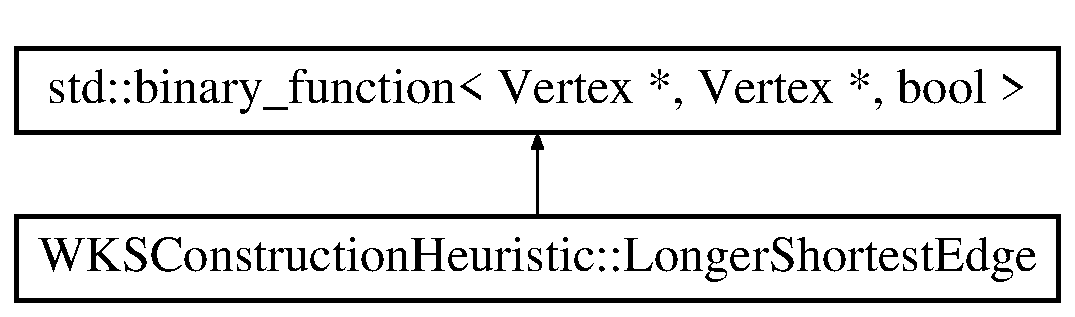
\includegraphics[height=2.000000cm]{classWKSConstructionHeuristic_1_1LongerShortestEdge}
\end{center}
\end{figure}
\subsection*{Public Member Functions}
\begin{DoxyCompactItemize}
\item 
bool \textbf{ operator()} (const \textbf{ Vertex} $\ast$v1, const \textbf{ Vertex} $\ast$v2)
\end{DoxyCompactItemize}


\subsection{Detailed Description}
lse(v1, v2) is true if the length of the shortest edge of v1 is greater than the length of the shortest edge of v2. If a vertex has Degree 0, the length of its shortest edge is defined to be +\+Infinity. If both v1 and v2 have degree 0, then the vertex with the greater label is defined to have the \char`\"{}longer shortest edge\char`\"{}. 

\subsection{Member Function Documentation}
\mbox{\label{classWKSConstructionHeuristic_1_1LongerShortestEdge_ae3ea58e171cf43e75e217d4c15657244}} 
\index{W\+K\+S\+Construction\+Heuristic\+::\+Longer\+Shortest\+Edge@{W\+K\+S\+Construction\+Heuristic\+::\+Longer\+Shortest\+Edge}!operator()@{operator()}}
\index{operator()@{operator()}!W\+K\+S\+Construction\+Heuristic\+::\+Longer\+Shortest\+Edge@{W\+K\+S\+Construction\+Heuristic\+::\+Longer\+Shortest\+Edge}}
\subsubsection{operator()()}
{\footnotesize\ttfamily bool W\+K\+S\+Construction\+Heuristic\+::\+Longer\+Shortest\+Edge\+::operator() (\begin{DoxyParamCaption}\item[{const \textbf{ Vertex} $\ast$}]{v1,  }\item[{const \textbf{ Vertex} $\ast$}]{v2 }\end{DoxyParamCaption})}



The documentation for this class was generated from the following files\+:\begin{DoxyCompactItemize}
\item 
\textbf{ W\+K\+S\+Construction\+Heuristic.\+h}\item 
\textbf{ W\+K\+S\+Construction\+Heuristic.\+cc}\end{DoxyCompactItemize}

\section{Matching Class Reference}
\label{classMatching}\index{Matching@{Matching}}


represent a matching on a graph  




{\ttfamily \#include $<$Matching.\+h$>$}

\subsection*{Classes}
\begin{DoxyCompactItemize}
\item 
class \textbf{ Vertex\+Info}
\begin{DoxyCompactList}\small\item\em contains information about a vertex that is possibly in a matching \end{DoxyCompactList}\end{DoxyCompactItemize}
\subsection*{Public Member Functions}
\begin{DoxyCompactItemize}
\item 
\textbf{ Matching} (\textbf{ Graph} $\ast$g, \textbf{ Progress\+Output} $\ast$po=N\+U\+LL)
\item 
\textbf{ $\sim$\+Matching} (void)
\item 
bool \textbf{ is\+Matched} (\textbf{ Vertex} $\ast$v) const
\item 
bool \textbf{ is\+Matched} (\textbf{ Vertex\+Label} vlbl) const
\item 
bool \textbf{ is\+Exposed} (\textbf{ Vertex} $\ast$v) const
\item 
bool \textbf{ is\+Exposed} (\textbf{ Vertex\+Label} vlbl) const
\item 
const \textbf{ Edge} $\ast$ \textbf{ get\+Matching\+Edge} (\textbf{ Vertex} $\ast$v) const
\item 
bool \textbf{ includes\+Edge} (const \textbf{ Edge} $\ast$e) const
\item 
bool \textbf{ includes\+Edge} (const \textbf{ Edge} \&e) const
\item 
unsigned long \textbf{ get\+Cardinality} (void) const
\item 
const std\+::list$<$ \textbf{ Vertex} $\ast$ $>$ \& \textbf{ get\+Exposed\+Vertices} (void) const
\item 
float \textbf{ get\+Matched\+Rate} (void) const
\item 
float \textbf{ get\+Avg\+Edge\+Weight} (void) const
\item 
const std\+::list$<$ \textbf{ Vertex} $\ast$ $>$ $\ast$ \textbf{ get\+Exposed\+Vertices\+Link} (void) const
\item 
void \textbf{ add\+Edge} (const \textbf{ Edge} \&e)
\item 
void \textbf{ add\+Edge} (\textbf{ Edge} $\ast$e)
\item 
void \textbf{ remove\+Edge} (const \textbf{ Edge} \&e)
\item 
const std\+::list$<$ \textbf{ Edge} $\ast$ $>$ \& \textbf{ get\+Edges} (void) const
\item 
\textbf{ Matching} \& \textbf{ augment} (const \textbf{ Edge} $\ast$$\ast$path, unsigned long len)
\item 
\textbf{ Matching} \& \textbf{ augment} (const std\+::vector$<$ \textbf{ Edge} $\ast$$>$ \&path)
\item 
void \textbf{ print\+Verbose\+Info} (void) const
\item 
bool \textbf{ check} (void) const
\item 
bool \textbf{ check\+\_\+\+Matching\+Edges\+\_\+vs\+\_\+\+Vertex\+Information} (void) const
\item 
bool \textbf{ check\+\_\+\+Exposed\+Vertices\+\_\+vs\+\_\+\+Vertex\+Information} (void) const
\item 
bool \textbf{ check\+\_\+\+Vertex\+Information\+\_\+\+Integrity} (void) const
\item 
bool \textbf{ check\+\_\+\+Valid\+Aug\+Path} (const std\+::vector$<$ \textbf{ Edge} $\ast$$>$ \&path) const
\end{DoxyCompactItemize}
\subsection*{Private Member Functions}
\begin{DoxyCompactItemize}
\item 
void \textbf{ set\+Cardinality} (unsigned long c)
\end{DoxyCompactItemize}
\subsection*{Private Attributes}
\begin{DoxyCompactItemize}
\item 
std\+::vector$<$ \textbf{ Vertex\+Info} $>$ \textbf{ Vertex\+Information}
\begin{DoxyCompactList}\small\item\em contains a \doxyref{Vertex\+Info}{p.}{classMatching_1_1VertexInfo} object for every vertex \end{DoxyCompactList}\item 
std\+::list$<$ \textbf{ Vertex} $\ast$ $>$ \textbf{ Exposed\+Vertices}
\begin{DoxyCompactList}\small\item\em the std\+::list of all exposed vertices \end{DoxyCompactList}\item 
std\+::list$<$ \textbf{ Edge} $\ast$ $>$ \textbf{ Matching\+Edges}
\begin{DoxyCompactList}\small\item\em the std\+::list of all edges in the matching \end{DoxyCompactList}\item 
unsigned long \textbf{ Cardinality}
\begin{DoxyCompactList}\small\item\em the number of edges in the matching \end{DoxyCompactList}\item 
\textbf{ Graph} $\ast$ \textbf{ The\+Graph}
\begin{DoxyCompactList}\small\item\em the graph underlying this \doxyref{Matching}{p.}{classMatching} \end{DoxyCompactList}\item 
\textbf{ Progress\+Output} $\ast$ \textbf{ Pr\+Out}
\begin{DoxyCompactList}\small\item\em the \doxyref{Progress\+Output}{p.}{classProgressOutput} object that will print the number of matched vertices (as percentage) \end{DoxyCompactList}\end{DoxyCompactItemize}


\subsection{Detailed Description}
A \doxyref{Matching}{p.}{classMatching} object will copy all Edges that are passed to it and will take care of them, i.\+e. delete them if they are no longer used. Edges do only \char`\"{}leave\char`\"{} a \doxyref{Matching}{p.}{classMatching} object as const pointers. 

\subsection{Constructor \& Destructor Documentation}
\mbox{\label{classMatching_aed84a04e309df94f8eb9005ffe957bbd}} 
\index{Matching@{Matching}!Matching@{Matching}}
\index{Matching@{Matching}!Matching@{Matching}}
\subsubsection{Matching()}
{\footnotesize\ttfamily Matching\+::\+Matching (\begin{DoxyParamCaption}\item[{\textbf{ Graph} $\ast$}]{g,  }\item[{\textbf{ Progress\+Output} $\ast$}]{po = {\ttfamily NULL} }\end{DoxyParamCaption})}

create an empty matching that is ready for adding and augmenting 
\begin{DoxyParams}{Parameters}
{\em g} & the underlying graph \\
\hline
{\em po} & a \doxyref{Progress\+Output}{p.}{classProgressOutput} object that will print the number of matched vertices (in percent) \\
\hline
\end{DoxyParams}
\mbox{\label{classMatching_ad2d812a2bf359a0aba56c4b010d593ca}} 
\index{Matching@{Matching}!````~Matching@{$\sim$\+Matching}}
\index{````~Matching@{$\sim$\+Matching}!Matching@{Matching}}
\subsubsection{$\sim$\+Matching()}
{\footnotesize\ttfamily Matching\+::$\sim$\+Matching (\begin{DoxyParamCaption}\item[{void}]{ }\end{DoxyParamCaption})}



\subsection{Member Function Documentation}
\mbox{\label{classMatching_a6c838465213fedaf6fc3604498bc4872}} 
\index{Matching@{Matching}!add\+Edge@{add\+Edge}}
\index{add\+Edge@{add\+Edge}!Matching@{Matching}}
\subsubsection{add\+Edge()\hspace{0.1cm}{\footnotesize\ttfamily [1/2]}}
{\footnotesize\ttfamily void Matching\+::add\+Edge (\begin{DoxyParamCaption}\item[{const \textbf{ Edge} \&}]{e }\end{DoxyParamCaption})}

add an edge to the matching 
\begin{DoxyParams}{Parameters}
{\em e} & the edge to add.\\
\hline
\end{DoxyParams}
For e=(v1,v2)\+: neither v1 nor v2 are allowed to be adjacent to an edge that is already in the matching, \mbox{\label{classMatching_a96c361574c82870fb2def9ee837a661b}} 
\index{Matching@{Matching}!add\+Edge@{add\+Edge}}
\index{add\+Edge@{add\+Edge}!Matching@{Matching}}
\subsubsection{add\+Edge()\hspace{0.1cm}{\footnotesize\ttfamily [2/2]}}
{\footnotesize\ttfamily void Matching\+::add\+Edge (\begin{DoxyParamCaption}\item[{\textbf{ Edge} $\ast$}]{e }\end{DoxyParamCaption})\hspace{0.3cm}{\ttfamily [inline]}}

\mbox{\label{classMatching_a129ad66579ab15131149c450f0d228bb}} 
\index{Matching@{Matching}!augment@{augment}}
\index{augment@{augment}!Matching@{Matching}}
\subsubsection{augment()\hspace{0.1cm}{\footnotesize\ttfamily [1/2]}}
{\footnotesize\ttfamily \textbf{ Matching} \& Matching\+::augment (\begin{DoxyParamCaption}\item[{const \textbf{ Edge} $\ast$$\ast$}]{path,  }\item[{unsigned long}]{len }\end{DoxyParamCaption})}

augment this matching along the given augmenting path 
\begin{DoxyParams}{Parameters}
{\em path} & an augmenting path \\
\hline
{\em len} & the length (number of edges) of the augmenting path\\
\hline
\end{DoxyParams}
An augementing path is a path where edges with odd indices (the first, third,...) are not in the matching and edges with even indices are and the path has an odd length. \mbox{\label{classMatching_af3007a9e1a3a012cab3d8f375e6c0b2f}} 
\index{Matching@{Matching}!augment@{augment}}
\index{augment@{augment}!Matching@{Matching}}
\subsubsection{augment()\hspace{0.1cm}{\footnotesize\ttfamily [2/2]}}
{\footnotesize\ttfamily \textbf{ Matching} \& Matching\+::augment (\begin{DoxyParamCaption}\item[{const std\+::vector$<$ \textbf{ Edge} $\ast$$>$ \&}]{path }\end{DoxyParamCaption})}

\mbox{\label{classMatching_a228050946f86494d0a55fcc87d62ea8d}} 
\index{Matching@{Matching}!check@{check}}
\index{check@{check}!Matching@{Matching}}
\subsubsection{check()}
{\footnotesize\ttfamily bool Matching\+::check (\begin{DoxyParamCaption}\item[{void}]{ }\end{DoxyParamCaption}) const}

\mbox{\label{classMatching_ad08e51d28eb8474e645149ba30378e35}} 
\index{Matching@{Matching}!check\+\_\+\+Exposed\+Vertices\+\_\+vs\+\_\+\+Vertex\+Information@{check\+\_\+\+Exposed\+Vertices\+\_\+vs\+\_\+\+Vertex\+Information}}
\index{check\+\_\+\+Exposed\+Vertices\+\_\+vs\+\_\+\+Vertex\+Information@{check\+\_\+\+Exposed\+Vertices\+\_\+vs\+\_\+\+Vertex\+Information}!Matching@{Matching}}
\subsubsection{check\+\_\+\+Exposed\+Vertices\+\_\+vs\+\_\+\+Vertex\+Information()}
{\footnotesize\ttfamily bool Matching\+::check\+\_\+\+Exposed\+Vertices\+\_\+vs\+\_\+\+Vertex\+Information (\begin{DoxyParamCaption}\item[{void}]{ }\end{DoxyParamCaption}) const}

\mbox{\label{classMatching_a238b7d528375a06d7e53786143e72450}} 
\index{Matching@{Matching}!check\+\_\+\+Matching\+Edges\+\_\+vs\+\_\+\+Vertex\+Information@{check\+\_\+\+Matching\+Edges\+\_\+vs\+\_\+\+Vertex\+Information}}
\index{check\+\_\+\+Matching\+Edges\+\_\+vs\+\_\+\+Vertex\+Information@{check\+\_\+\+Matching\+Edges\+\_\+vs\+\_\+\+Vertex\+Information}!Matching@{Matching}}
\subsubsection{check\+\_\+\+Matching\+Edges\+\_\+vs\+\_\+\+Vertex\+Information()}
{\footnotesize\ttfamily bool Matching\+::check\+\_\+\+Matching\+Edges\+\_\+vs\+\_\+\+Vertex\+Information (\begin{DoxyParamCaption}\item[{void}]{ }\end{DoxyParamCaption}) const}

\mbox{\label{classMatching_ace51856a8d01c60c3b0638118bfacba6}} 
\index{Matching@{Matching}!check\+\_\+\+Valid\+Aug\+Path@{check\+\_\+\+Valid\+Aug\+Path}}
\index{check\+\_\+\+Valid\+Aug\+Path@{check\+\_\+\+Valid\+Aug\+Path}!Matching@{Matching}}
\subsubsection{check\+\_\+\+Valid\+Aug\+Path()}
{\footnotesize\ttfamily bool Matching\+::check\+\_\+\+Valid\+Aug\+Path (\begin{DoxyParamCaption}\item[{const std\+::vector$<$ \textbf{ Edge} $\ast$$>$ \&}]{path }\end{DoxyParamCaption}) const}

\mbox{\label{classMatching_aac70adfc95547020b988cc99ff4f50a5}} 
\index{Matching@{Matching}!check\+\_\+\+Vertex\+Information\+\_\+\+Integrity@{check\+\_\+\+Vertex\+Information\+\_\+\+Integrity}}
\index{check\+\_\+\+Vertex\+Information\+\_\+\+Integrity@{check\+\_\+\+Vertex\+Information\+\_\+\+Integrity}!Matching@{Matching}}
\subsubsection{check\+\_\+\+Vertex\+Information\+\_\+\+Integrity()}
{\footnotesize\ttfamily bool Matching\+::check\+\_\+\+Vertex\+Information\+\_\+\+Integrity (\begin{DoxyParamCaption}\item[{void}]{ }\end{DoxyParamCaption}) const}

\mbox{\label{classMatching_aaae0ccd8440b174446959caeff5eb924}} 
\index{Matching@{Matching}!get\+Avg\+Edge\+Weight@{get\+Avg\+Edge\+Weight}}
\index{get\+Avg\+Edge\+Weight@{get\+Avg\+Edge\+Weight}!Matching@{Matching}}
\subsubsection{get\+Avg\+Edge\+Weight()}
{\footnotesize\ttfamily float Matching\+::get\+Avg\+Edge\+Weight (\begin{DoxyParamCaption}\item[{void}]{ }\end{DoxyParamCaption}) const}

get the average weight of all edges that are in this matching \mbox{\label{classMatching_a0ef0a64e0f3e321b28c78617a65af749}} 
\index{Matching@{Matching}!get\+Cardinality@{get\+Cardinality}}
\index{get\+Cardinality@{get\+Cardinality}!Matching@{Matching}}
\subsubsection{get\+Cardinality()}
{\footnotesize\ttfamily unsigned long Matching\+::get\+Cardinality (\begin{DoxyParamCaption}\item[{void}]{ }\end{DoxyParamCaption}) const\hspace{0.3cm}{\ttfamily [inline]}}

get the cardinality (the number of matched edges) \mbox{\label{classMatching_af8e8287e2ef659ce956d832f31bd77be}} 
\index{Matching@{Matching}!get\+Edges@{get\+Edges}}
\index{get\+Edges@{get\+Edges}!Matching@{Matching}}
\subsubsection{get\+Edges()}
{\footnotesize\ttfamily const std\+::list$<$\textbf{ Edge}$\ast$$>$\& Matching\+::get\+Edges (\begin{DoxyParamCaption}\item[{void}]{ }\end{DoxyParamCaption}) const\hspace{0.3cm}{\ttfamily [inline]}}

get the list of all edges in this matching \mbox{\label{classMatching_a1148deb78c1929aa07ce128332e3ba0f}} 
\index{Matching@{Matching}!get\+Exposed\+Vertices@{get\+Exposed\+Vertices}}
\index{get\+Exposed\+Vertices@{get\+Exposed\+Vertices}!Matching@{Matching}}
\subsubsection{get\+Exposed\+Vertices()}
{\footnotesize\ttfamily const std\+::list$<$\textbf{ Vertex}$\ast$$>$\& Matching\+::get\+Exposed\+Vertices (\begin{DoxyParamCaption}\item[{void}]{ }\end{DoxyParamCaption}) const\hspace{0.3cm}{\ttfamily [inline]}}

\mbox{\label{classMatching_a157a6f2ac29fa66e99218b6e7693c189}} 
\index{Matching@{Matching}!get\+Exposed\+Vertices\+Link@{get\+Exposed\+Vertices\+Link}}
\index{get\+Exposed\+Vertices\+Link@{get\+Exposed\+Vertices\+Link}!Matching@{Matching}}
\subsubsection{get\+Exposed\+Vertices\+Link()}
{\footnotesize\ttfamily const std\+::list$<$\textbf{ Vertex}$\ast$$>$$\ast$ Matching\+::get\+Exposed\+Vertices\+Link (\begin{DoxyParamCaption}\item[{void}]{ }\end{DoxyParamCaption}) const\hspace{0.3cm}{\ttfamily [inline]}}

get access to the std\+::list of exposed vertices \begin{DoxyReturn}{Returns}
a pointer to the std\+::list of exposed vertices in this matching.
\end{DoxyReturn}
The std\+::list that is pointed to by return value contains the exposed vertices even after augment has been called (it is the Exposed\+Vertices member) an arbitrary number of times. \mbox{\label{classMatching_a1a4ef03ce17f0161c06f78a199b0f4f1}} 
\index{Matching@{Matching}!get\+Matched\+Rate@{get\+Matched\+Rate}}
\index{get\+Matched\+Rate@{get\+Matched\+Rate}!Matching@{Matching}}
\subsubsection{get\+Matched\+Rate()}
{\footnotesize\ttfamily float Matching\+::get\+Matched\+Rate (\begin{DoxyParamCaption}\item[{void}]{ }\end{DoxyParamCaption}) const}

get the rate of vertices of the underlying graph that are currently matched in this matching \begin{DoxyReturn}{Returns}
a value between 0 and 1 
\end{DoxyReturn}
\mbox{\label{classMatching_a994d4033a6ce0dc9b2d0ebfeb99abaad}} 
\index{Matching@{Matching}!get\+Matching\+Edge@{get\+Matching\+Edge}}
\index{get\+Matching\+Edge@{get\+Matching\+Edge}!Matching@{Matching}}
\subsubsection{get\+Matching\+Edge()}
{\footnotesize\ttfamily const \textbf{ Edge}$\ast$ Matching\+::get\+Matching\+Edge (\begin{DoxyParamCaption}\item[{\textbf{ Vertex} $\ast$}]{v }\end{DoxyParamCaption}) const\hspace{0.3cm}{\ttfamily [inline]}}

get the edge that is in the matching and adjacent to v \begin{DoxyReturn}{Returns}
the matched edge or N\+U\+LL if v is exposed 
\end{DoxyReturn}
\mbox{\label{classMatching_a5ab2b2d30f2a677b11748fd488363bd7}} 
\index{Matching@{Matching}!includes\+Edge@{includes\+Edge}}
\index{includes\+Edge@{includes\+Edge}!Matching@{Matching}}
\subsubsection{includes\+Edge()\hspace{0.1cm}{\footnotesize\ttfamily [1/2]}}
{\footnotesize\ttfamily bool Matching\+::includes\+Edge (\begin{DoxyParamCaption}\item[{const \textbf{ Edge} $\ast$}]{e }\end{DoxyParamCaption}) const\hspace{0.3cm}{\ttfamily [inline]}}

does this matching include the edge e ? \begin{DoxyReturn}{Returns}
true iff the edge e is element of this matching 
\end{DoxyReturn}
\mbox{\label{classMatching_a65016580feb104843b1c299481e3bb15}} 
\index{Matching@{Matching}!includes\+Edge@{includes\+Edge}}
\index{includes\+Edge@{includes\+Edge}!Matching@{Matching}}
\subsubsection{includes\+Edge()\hspace{0.1cm}{\footnotesize\ttfamily [2/2]}}
{\footnotesize\ttfamily bool Matching\+::includes\+Edge (\begin{DoxyParamCaption}\item[{const \textbf{ Edge} \&}]{e }\end{DoxyParamCaption}) const}

\mbox{\label{classMatching_a1aa623dc0383ad7e42cee2fa509d741b}} 
\index{Matching@{Matching}!is\+Exposed@{is\+Exposed}}
\index{is\+Exposed@{is\+Exposed}!Matching@{Matching}}
\subsubsection{is\+Exposed()\hspace{0.1cm}{\footnotesize\ttfamily [1/2]}}
{\footnotesize\ttfamily bool Matching\+::is\+Exposed (\begin{DoxyParamCaption}\item[{\textbf{ Vertex} $\ast$}]{v }\end{DoxyParamCaption}) const\hspace{0.3cm}{\ttfamily [inline]}}

returns true iff the vertex v is exposed (not matched) in this matching. \mbox{\label{classMatching_a666297ec929bc0663a2177a8d6e25099}} 
\index{Matching@{Matching}!is\+Exposed@{is\+Exposed}}
\index{is\+Exposed@{is\+Exposed}!Matching@{Matching}}
\subsubsection{is\+Exposed()\hspace{0.1cm}{\footnotesize\ttfamily [2/2]}}
{\footnotesize\ttfamily bool Matching\+::is\+Exposed (\begin{DoxyParamCaption}\item[{\textbf{ Vertex\+Label}}]{vlbl }\end{DoxyParamCaption}) const\hspace{0.3cm}{\ttfamily [inline]}}

returns true iff the vertex with the label vlbl is exposed (not matched) in this matching. \mbox{\label{classMatching_a0c1b2558dc7055812271e8a26f8c7bbf}} 
\index{Matching@{Matching}!is\+Matched@{is\+Matched}}
\index{is\+Matched@{is\+Matched}!Matching@{Matching}}
\subsubsection{is\+Matched()\hspace{0.1cm}{\footnotesize\ttfamily [1/2]}}
{\footnotesize\ttfamily bool Matching\+::is\+Matched (\begin{DoxyParamCaption}\item[{\textbf{ Vertex} $\ast$}]{v }\end{DoxyParamCaption}) const\hspace{0.3cm}{\ttfamily [inline]}}

returns true iff the vertex v is matched in this matching. \mbox{\label{classMatching_ab3498a477d0f76d10968f7679b34f5cb}} 
\index{Matching@{Matching}!is\+Matched@{is\+Matched}}
\index{is\+Matched@{is\+Matched}!Matching@{Matching}}
\subsubsection{is\+Matched()\hspace{0.1cm}{\footnotesize\ttfamily [2/2]}}
{\footnotesize\ttfamily bool Matching\+::is\+Matched (\begin{DoxyParamCaption}\item[{\textbf{ Vertex\+Label}}]{vlbl }\end{DoxyParamCaption}) const\hspace{0.3cm}{\ttfamily [inline]}}

returns true iff the vertex with the label vlbl is matched in this matching. \mbox{\label{classMatching_a5bdd63b1f2e52410dae97c19854a3117}} 
\index{Matching@{Matching}!print\+Verbose\+Info@{print\+Verbose\+Info}}
\index{print\+Verbose\+Info@{print\+Verbose\+Info}!Matching@{Matching}}
\subsubsection{print\+Verbose\+Info()}
{\footnotesize\ttfamily void Matching\+::print\+Verbose\+Info (\begin{DoxyParamCaption}\item[{void}]{ }\end{DoxyParamCaption}) const}

\mbox{\label{classMatching_a050930214af9313531a041cd7b0cfdc9}} 
\index{Matching@{Matching}!remove\+Edge@{remove\+Edge}}
\index{remove\+Edge@{remove\+Edge}!Matching@{Matching}}
\subsubsection{remove\+Edge()}
{\footnotesize\ttfamily void Matching\+::remove\+Edge (\begin{DoxyParamCaption}\item[{const \textbf{ Edge} \&}]{e }\end{DoxyParamCaption})}

remove an edge from the matching 
\begin{DoxyParams}{Parameters}
{\em e} & the edge to remove\\
\hline
\end{DoxyParams}
The edge e {\itshape must} be in this matching \mbox{\label{classMatching_abb3bd68cfac697812d6719cc72a42915}} 
\index{Matching@{Matching}!set\+Cardinality@{set\+Cardinality}}
\index{set\+Cardinality@{set\+Cardinality}!Matching@{Matching}}
\subsubsection{set\+Cardinality()}
{\footnotesize\ttfamily void Matching\+::set\+Cardinality (\begin{DoxyParamCaption}\item[{unsigned long}]{c }\end{DoxyParamCaption})\hspace{0.3cm}{\ttfamily [private]}}

set the cardinality (thereby updating Pr\+Out) 

\subsection{Member Data Documentation}
\mbox{\label{classMatching_a0010374751f5cb6a24a103d020125df2}} 
\index{Matching@{Matching}!Cardinality@{Cardinality}}
\index{Cardinality@{Cardinality}!Matching@{Matching}}
\subsubsection{Cardinality}
{\footnotesize\ttfamily unsigned long Matching\+::\+Cardinality\hspace{0.3cm}{\ttfamily [private]}}

\mbox{\label{classMatching_ad13336c41a30e91d0e43d76d9a3472d0}} 
\index{Matching@{Matching}!Exposed\+Vertices@{Exposed\+Vertices}}
\index{Exposed\+Vertices@{Exposed\+Vertices}!Matching@{Matching}}
\subsubsection{Exposed\+Vertices}
{\footnotesize\ttfamily std\+::list$<$\textbf{ Vertex}$\ast$$>$ Matching\+::\+Exposed\+Vertices\hspace{0.3cm}{\ttfamily [private]}}

\mbox{\label{classMatching_a101468aa7aa0d515d5f26a90aff23635}} 
\index{Matching@{Matching}!Matching\+Edges@{Matching\+Edges}}
\index{Matching\+Edges@{Matching\+Edges}!Matching@{Matching}}
\subsubsection{Matching\+Edges}
{\footnotesize\ttfamily std\+::list$<$\textbf{ Edge}$\ast$$>$ Matching\+::\+Matching\+Edges\hspace{0.3cm}{\ttfamily [private]}}

\mbox{\label{classMatching_a557079f39cb4955db24659100f391eef}} 
\index{Matching@{Matching}!Pr\+Out@{Pr\+Out}}
\index{Pr\+Out@{Pr\+Out}!Matching@{Matching}}
\subsubsection{Pr\+Out}
{\footnotesize\ttfamily \textbf{ Progress\+Output}$\ast$ Matching\+::\+Pr\+Out\hspace{0.3cm}{\ttfamily [private]}}

\mbox{\label{classMatching_aeca9faeb654b61cd465de583e57ff991}} 
\index{Matching@{Matching}!The\+Graph@{The\+Graph}}
\index{The\+Graph@{The\+Graph}!Matching@{Matching}}
\subsubsection{The\+Graph}
{\footnotesize\ttfamily \textbf{ Graph}$\ast$ Matching\+::\+The\+Graph\hspace{0.3cm}{\ttfamily [private]}}

\mbox{\label{classMatching_a0942e9b5f7ebac36164d003fd84d7f32}} 
\index{Matching@{Matching}!Vertex\+Information@{Vertex\+Information}}
\index{Vertex\+Information@{Vertex\+Information}!Matching@{Matching}}
\subsubsection{Vertex\+Information}
{\footnotesize\ttfamily std\+::vector$<$\textbf{ Vertex\+Info}$>$ Matching\+::\+Vertex\+Information\hspace{0.3cm}{\ttfamily [private]}}



The documentation for this class was generated from the following files\+:\begin{DoxyCompactItemize}
\item 
\textbf{ Matching.\+h}\item 
\textbf{ Matching.\+cc}\end{DoxyCompactItemize}

\section{Matching\+Algorithm Class Reference}
\label{classMatchingAlgorithm}\index{Matching\+Algorithm@{Matching\+Algorithm}}


{\ttfamily \#include $<$Matching\+Algorithm.\+h$>$}

Inheritance diagram for Matching\+Algorithm\+:\begin{figure}[H]
\begin{center}
\leavevmode
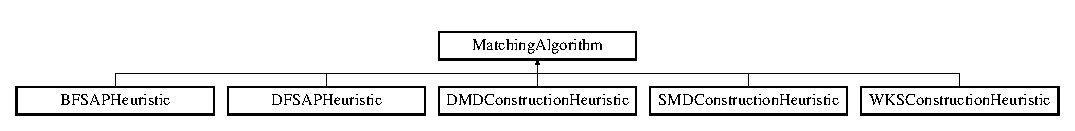
\includegraphics[height=1.317647cm]{classMatchingAlgorithm}
\end{center}
\end{figure}
\subsection*{Public Member Functions}
\begin{DoxyCompactItemize}
\item 
\textbf{ Matching\+Algorithm} (\textbf{ Graph} $\ast$g, \textbf{ Matching} $\ast$m, float goal)
\item 
virtual \textbf{ $\sim$\+Matching\+Algorithm} (void)
\item 
virtual void \textbf{ run} (void)=0
\item 
\textbf{ Matching} $\ast$ \textbf{ get\+Matching} (void) const
\item 
void \textbf{ set\+Goal} (float goal)
\item 
virtual const char $\ast$ \textbf{ get\+Name} (void) const =0
\end{DoxyCompactItemize}
\subsection*{Protected Attributes}
\begin{DoxyCompactItemize}
\item 
\textbf{ Graph} $\ast$ \textbf{ The\+Graph}
\item 
\textbf{ Matching} $\ast$ \textbf{ The\+Matching}
\item 
unsigned long \textbf{ Cardinality\+Goal}
\end{DoxyCompactItemize}


\subsection{Constructor \& Destructor Documentation}
\mbox{\label{classMatchingAlgorithm_ae8cd854b438d0d4b90dce63296a29961}} 
\index{Matching\+Algorithm@{Matching\+Algorithm}!Matching\+Algorithm@{Matching\+Algorithm}}
\index{Matching\+Algorithm@{Matching\+Algorithm}!Matching\+Algorithm@{Matching\+Algorithm}}
\subsubsection{Matching\+Algorithm()}
{\footnotesize\ttfamily Matching\+Algorithm\+::\+Matching\+Algorithm (\begin{DoxyParamCaption}\item[{\textbf{ Graph} $\ast$}]{g,  }\item[{\textbf{ Matching} $\ast$}]{m,  }\item[{float}]{goal }\end{DoxyParamCaption})}

\mbox{\label{classMatchingAlgorithm_a263bc490ed5abf59bb6fa0336cacd9da}} 
\index{Matching\+Algorithm@{Matching\+Algorithm}!````~Matching\+Algorithm@{$\sim$\+Matching\+Algorithm}}
\index{````~Matching\+Algorithm@{$\sim$\+Matching\+Algorithm}!Matching\+Algorithm@{Matching\+Algorithm}}
\subsubsection{$\sim$\+Matching\+Algorithm()}
{\footnotesize\ttfamily virtual Matching\+Algorithm\+::$\sim$\+Matching\+Algorithm (\begin{DoxyParamCaption}\item[{void}]{ }\end{DoxyParamCaption})\hspace{0.3cm}{\ttfamily [inline]}, {\ttfamily [virtual]}}



\subsection{Member Function Documentation}
\mbox{\label{classMatchingAlgorithm_aa098c67b241f6441539faea7862822a8}} 
\index{Matching\+Algorithm@{Matching\+Algorithm}!get\+Matching@{get\+Matching}}
\index{get\+Matching@{get\+Matching}!Matching\+Algorithm@{Matching\+Algorithm}}
\subsubsection{get\+Matching()}
{\footnotesize\ttfamily \textbf{ Matching}$\ast$ Matching\+Algorithm\+::get\+Matching (\begin{DoxyParamCaption}\item[{void}]{ }\end{DoxyParamCaption}) const\hspace{0.3cm}{\ttfamily [inline]}}

\mbox{\label{classMatchingAlgorithm_a7305edae5d74e91987bcf983b2a1171a}} 
\index{Matching\+Algorithm@{Matching\+Algorithm}!get\+Name@{get\+Name}}
\index{get\+Name@{get\+Name}!Matching\+Algorithm@{Matching\+Algorithm}}
\subsubsection{get\+Name()}
{\footnotesize\ttfamily virtual const char$\ast$ Matching\+Algorithm\+::get\+Name (\begin{DoxyParamCaption}\item[{void}]{ }\end{DoxyParamCaption}) const\hspace{0.3cm}{\ttfamily [pure virtual]}}



Implemented in \textbf{ W\+K\+S\+Construction\+Heuristic} \doxyref{}{p.}{classWKSConstructionHeuristic_a279664d019277e218ea026d436ecd549}, \textbf{ D\+F\+S\+A\+P\+Heuristic} \doxyref{}{p.}{classDFSAPHeuristic_afd3814466a9968e66558451ae0a0c611}, \textbf{ B\+F\+S\+A\+P\+Heuristic} \doxyref{}{p.}{classBFSAPHeuristic_afbd3a55843232ba22bea3360e6009a97}, \textbf{ D\+M\+D\+Construction\+Heuristic} \doxyref{}{p.}{classDMDConstructionHeuristic_a0ee1864e50b3478d6cccdd18f2502c54}, and \textbf{ S\+M\+D\+Construction\+Heuristic} \doxyref{}{p.}{classSMDConstructionHeuristic_a9e5bd0cdb6c2318d791fa9d38406dc84}.

\mbox{\label{classMatchingAlgorithm_aeea6c808daf03fd788c9a9feea885c41}} 
\index{Matching\+Algorithm@{Matching\+Algorithm}!run@{run}}
\index{run@{run}!Matching\+Algorithm@{Matching\+Algorithm}}
\subsubsection{run()}
{\footnotesize\ttfamily virtual void Matching\+Algorithm\+::run (\begin{DoxyParamCaption}\item[{void}]{ }\end{DoxyParamCaption})\hspace{0.3cm}{\ttfamily [pure virtual]}}



Implemented in \textbf{ D\+F\+S\+A\+P\+Heuristic} \doxyref{}{p.}{classDFSAPHeuristic_a6be8de5d724975d145500fc7a1f12198}, \textbf{ W\+K\+S\+Construction\+Heuristic} \doxyref{}{p.}{classWKSConstructionHeuristic_a04c931636b6e457493b6bc25697f98fb}, \textbf{ B\+F\+S\+A\+P\+Heuristic} \doxyref{}{p.}{classBFSAPHeuristic_a2b12948841049cfca3e6d634d793c510}, \textbf{ D\+M\+D\+Construction\+Heuristic} \doxyref{}{p.}{classDMDConstructionHeuristic_a49dd3ba3c89b0993922918379d3d3240}, and \textbf{ S\+M\+D\+Construction\+Heuristic} \doxyref{}{p.}{classSMDConstructionHeuristic_a34f0fc8df70751b17badb578be25d5a0}.

\mbox{\label{classMatchingAlgorithm_ae6fa3917ebacc51dcf465a173d8d42a3}} 
\index{Matching\+Algorithm@{Matching\+Algorithm}!set\+Goal@{set\+Goal}}
\index{set\+Goal@{set\+Goal}!Matching\+Algorithm@{Matching\+Algorithm}}
\subsubsection{set\+Goal()}
{\footnotesize\ttfamily void Matching\+Algorithm\+::set\+Goal (\begin{DoxyParamCaption}\item[{float}]{goal }\end{DoxyParamCaption})}



\subsection{Member Data Documentation}
\mbox{\label{classMatchingAlgorithm_aec9ec46a32f1afcd67b338d54ddb0e1c}} 
\index{Matching\+Algorithm@{Matching\+Algorithm}!Cardinality\+Goal@{Cardinality\+Goal}}
\index{Cardinality\+Goal@{Cardinality\+Goal}!Matching\+Algorithm@{Matching\+Algorithm}}
\subsubsection{Cardinality\+Goal}
{\footnotesize\ttfamily unsigned long Matching\+Algorithm\+::\+Cardinality\+Goal\hspace{0.3cm}{\ttfamily [protected]}}

\mbox{\label{classMatchingAlgorithm_a3af20bc23311e6165f81d5064f1d0404}} 
\index{Matching\+Algorithm@{Matching\+Algorithm}!The\+Graph@{The\+Graph}}
\index{The\+Graph@{The\+Graph}!Matching\+Algorithm@{Matching\+Algorithm}}
\subsubsection{The\+Graph}
{\footnotesize\ttfamily \textbf{ Graph}$\ast$ Matching\+Algorithm\+::\+The\+Graph\hspace{0.3cm}{\ttfamily [protected]}}

\mbox{\label{classMatchingAlgorithm_a7f048641a6db4e92258f7b118fac33b0}} 
\index{Matching\+Algorithm@{Matching\+Algorithm}!The\+Matching@{The\+Matching}}
\index{The\+Matching@{The\+Matching}!Matching\+Algorithm@{Matching\+Algorithm}}
\subsubsection{The\+Matching}
{\footnotesize\ttfamily \textbf{ Matching}$\ast$ Matching\+Algorithm\+::\+The\+Matching\hspace{0.3cm}{\ttfamily [protected]}}



The documentation for this class was generated from the following files\+:\begin{DoxyCompactItemize}
\item 
\textbf{ Matching\+Algorithm.\+h}\item 
\textbf{ Matching\+Algorithm.\+cc}\end{DoxyCompactItemize}

\section{Matching\+Test Class Reference}
\label{classMatchingTest}\index{Matching\+Test@{Matching\+Test}}


{\ttfamily \#include $<$Matching\+Test.\+h$>$}

Inheritance diagram for Matching\+Test\+:\begin{figure}[H]
\begin{center}
\leavevmode
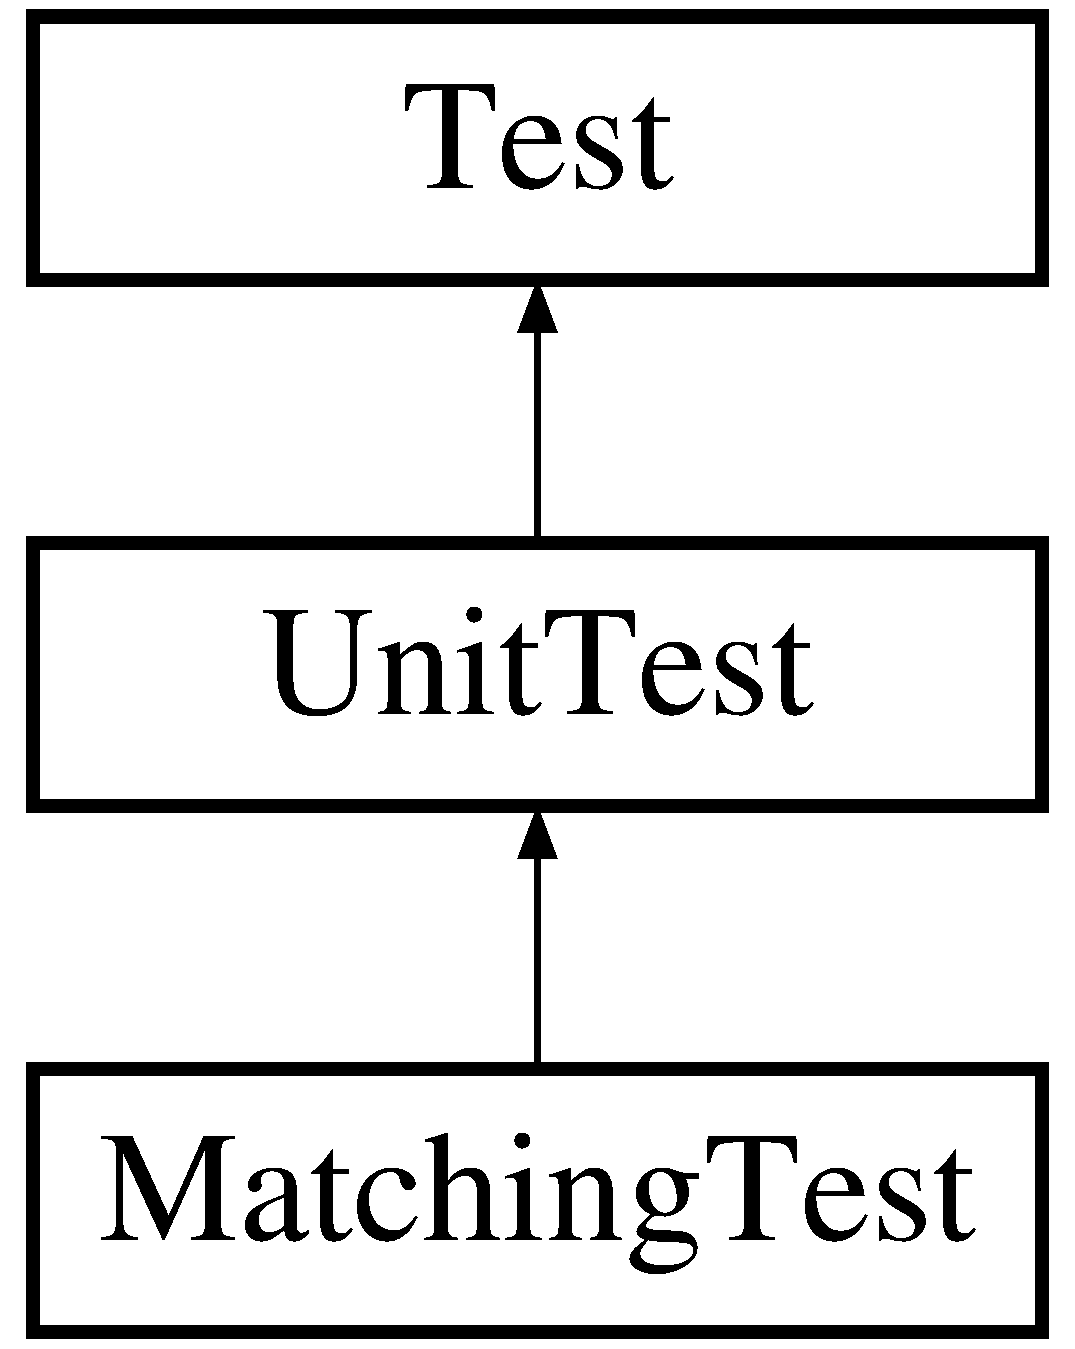
\includegraphics[height=3.000000cm]{classMatchingTest}
\end{center}
\end{figure}
\subsection*{Public Member Functions}
\begin{DoxyCompactItemize}
\item 
\textbf{ Matching\+Test} (\textbf{ Test\+Suite} $\ast$s)
\item 
void \textbf{ setup} (void)
\item 
void \textbf{ cleanup} (void)
\item 
void \textbf{ test\+Add\+Remove\+Edge} (void)
\item 
void \textbf{ test\+Augmenting\+Path} (void)
\end{DoxyCompactItemize}
\subsection*{Private Attributes}
\begin{DoxyCompactItemize}
\item 
\textbf{ Bit\+String} $\ast$ \textbf{ bs1}
\item 
\textbf{ Bit\+String} $\ast$ \textbf{ bs2}
\item 
\textbf{ Cvr\+Stg\+File} $\ast$ \textbf{ f1}
\item 
\textbf{ Cvr\+Stg\+File} $\ast$ \textbf{ f2}
\item 
\textbf{ Selector} $\ast$ \textbf{ s1}
\item 
\textbf{ Selector} $\ast$ \textbf{ s2}
\item 
\textbf{ Graph} $\ast$ \textbf{ g1}
\item 
\textbf{ Graph} $\ast$ \textbf{ g2}
\item 
\textbf{ Matching} $\ast$ \textbf{ m1}
\item 
\textbf{ Matching} $\ast$ \textbf{ m2}
\item 
\textbf{ Globals} \textbf{ gl1}
\item 
\textbf{ Globals} \textbf{ gl2}
\end{DoxyCompactItemize}
\subsection*{Additional Inherited Members}


\subsection{Constructor \& Destructor Documentation}
\mbox{\label{classMatchingTest_a4d394ef9c56f94617b25368018039a69}} 
\index{Matching\+Test@{Matching\+Test}!Matching\+Test@{Matching\+Test}}
\index{Matching\+Test@{Matching\+Test}!Matching\+Test@{Matching\+Test}}
\subsubsection{Matching\+Test()}
{\footnotesize\ttfamily Matching\+Test\+::\+Matching\+Test (\begin{DoxyParamCaption}\item[{\textbf{ Test\+Suite} $\ast$}]{s }\end{DoxyParamCaption})}



\subsection{Member Function Documentation}
\mbox{\label{classMatchingTest_aec8e791424a85a87a1b2768b1263e11a}} 
\index{Matching\+Test@{Matching\+Test}!cleanup@{cleanup}}
\index{cleanup@{cleanup}!Matching\+Test@{Matching\+Test}}
\subsubsection{cleanup()}
{\footnotesize\ttfamily void Matching\+Test\+::cleanup (\begin{DoxyParamCaption}\item[{void}]{ }\end{DoxyParamCaption})\hspace{0.3cm}{\ttfamily [virtual]}}

cleanup the unit test -\/ called after run 

Reimplemented from \textbf{ Unit\+Test} \doxyref{}{p.}{classUnitTest_adf77efe972ee4a766d94e3f7ddc193ad}.

\mbox{\label{classMatchingTest_a7eaacade93babf431d433f12fc8beac5}} 
\index{Matching\+Test@{Matching\+Test}!setup@{setup}}
\index{setup@{setup}!Matching\+Test@{Matching\+Test}}
\subsubsection{setup()}
{\footnotesize\ttfamily void Matching\+Test\+::setup (\begin{DoxyParamCaption}\item[{void}]{ }\end{DoxyParamCaption})\hspace{0.3cm}{\ttfamily [virtual]}}

setup the unit test -\/ called before run

\doxyref{Unit\+Test\+::setup}{p.}{classUnitTest_ad73fdf9012b651047ea001d21f9d27ad} will (together with \doxyref{Unit\+Test\+::cleanup}{p.}{classUnitTest_adf77efe972ee4a766d94e3f7ddc193ad}) save and restore the object stored in Globs so they should be called from the corresponding functions in the derived object if the derived unit test manipulates the Globs object. 

Reimplemented from \textbf{ Unit\+Test} \doxyref{}{p.}{classUnitTest_ad73fdf9012b651047ea001d21f9d27ad}.

\mbox{\label{classMatchingTest_aed472fcd05151da9c8ab8b25b8f0f895}} 
\index{Matching\+Test@{Matching\+Test}!test\+Add\+Remove\+Edge@{test\+Add\+Remove\+Edge}}
\index{test\+Add\+Remove\+Edge@{test\+Add\+Remove\+Edge}!Matching\+Test@{Matching\+Test}}
\subsubsection{test\+Add\+Remove\+Edge()}
{\footnotesize\ttfamily void Matching\+Test\+::test\+Add\+Remove\+Edge (\begin{DoxyParamCaption}\item[{void}]{ }\end{DoxyParamCaption})}

\mbox{\label{classMatchingTest_aca11568523fd62fca3df73ddad7d7adb}} 
\index{Matching\+Test@{Matching\+Test}!test\+Augmenting\+Path@{test\+Augmenting\+Path}}
\index{test\+Augmenting\+Path@{test\+Augmenting\+Path}!Matching\+Test@{Matching\+Test}}
\subsubsection{test\+Augmenting\+Path()}
{\footnotesize\ttfamily void Matching\+Test\+::test\+Augmenting\+Path (\begin{DoxyParamCaption}\item[{void}]{ }\end{DoxyParamCaption})}



\subsection{Member Data Documentation}
\mbox{\label{classMatchingTest_a7a2b5c230513aa99f584aa873ad33504}} 
\index{Matching\+Test@{Matching\+Test}!bs1@{bs1}}
\index{bs1@{bs1}!Matching\+Test@{Matching\+Test}}
\subsubsection{bs1}
{\footnotesize\ttfamily \textbf{ Bit\+String}$\ast$ Matching\+Test\+::bs1\hspace{0.3cm}{\ttfamily [private]}}

\mbox{\label{classMatchingTest_a1830c65ecd9e5644fe09d282fabfd4a1}} 
\index{Matching\+Test@{Matching\+Test}!bs2@{bs2}}
\index{bs2@{bs2}!Matching\+Test@{Matching\+Test}}
\subsubsection{bs2}
{\footnotesize\ttfamily \textbf{ Bit\+String} $\ast$ Matching\+Test\+::bs2\hspace{0.3cm}{\ttfamily [private]}}

\mbox{\label{classMatchingTest_a8e8d178c38cf7965b5e03832e197f3e9}} 
\index{Matching\+Test@{Matching\+Test}!f1@{f1}}
\index{f1@{f1}!Matching\+Test@{Matching\+Test}}
\subsubsection{f1}
{\footnotesize\ttfamily \textbf{ Cvr\+Stg\+File}$\ast$ Matching\+Test\+::f1\hspace{0.3cm}{\ttfamily [private]}}

\mbox{\label{classMatchingTest_abbbf61ae7d812f5877f5b973a4cbe0fd}} 
\index{Matching\+Test@{Matching\+Test}!f2@{f2}}
\index{f2@{f2}!Matching\+Test@{Matching\+Test}}
\subsubsection{f2}
{\footnotesize\ttfamily \textbf{ Cvr\+Stg\+File} $\ast$ Matching\+Test\+::f2\hspace{0.3cm}{\ttfamily [private]}}

\mbox{\label{classMatchingTest_ace10b42f4548578409ed230d955bdd98}} 
\index{Matching\+Test@{Matching\+Test}!g1@{g1}}
\index{g1@{g1}!Matching\+Test@{Matching\+Test}}
\subsubsection{g1}
{\footnotesize\ttfamily \textbf{ Graph}$\ast$ Matching\+Test\+::g1\hspace{0.3cm}{\ttfamily [private]}}

\mbox{\label{classMatchingTest_ae37f6684d4d8bfb24f957ab2694e38c1}} 
\index{Matching\+Test@{Matching\+Test}!g2@{g2}}
\index{g2@{g2}!Matching\+Test@{Matching\+Test}}
\subsubsection{g2}
{\footnotesize\ttfamily \textbf{ Graph} $\ast$ Matching\+Test\+::g2\hspace{0.3cm}{\ttfamily [private]}}

\mbox{\label{classMatchingTest_ae46e4d93253d53e952c31490dfbec5ea}} 
\index{Matching\+Test@{Matching\+Test}!gl1@{gl1}}
\index{gl1@{gl1}!Matching\+Test@{Matching\+Test}}
\subsubsection{gl1}
{\footnotesize\ttfamily \textbf{ Globals} Matching\+Test\+::gl1\hspace{0.3cm}{\ttfamily [private]}}

\mbox{\label{classMatchingTest_af2dad0b76d944dac9e0cde6d38caae25}} 
\index{Matching\+Test@{Matching\+Test}!gl2@{gl2}}
\index{gl2@{gl2}!Matching\+Test@{Matching\+Test}}
\subsubsection{gl2}
{\footnotesize\ttfamily \textbf{ Globals} Matching\+Test\+::gl2\hspace{0.3cm}{\ttfamily [private]}}

\mbox{\label{classMatchingTest_adf09bdc08c2558566ae8197f0b26c1cf}} 
\index{Matching\+Test@{Matching\+Test}!m1@{m1}}
\index{m1@{m1}!Matching\+Test@{Matching\+Test}}
\subsubsection{m1}
{\footnotesize\ttfamily \textbf{ Matching}$\ast$ Matching\+Test\+::m1\hspace{0.3cm}{\ttfamily [private]}}

\mbox{\label{classMatchingTest_a7d65ff7b2744f7e57f598fa0b396271b}} 
\index{Matching\+Test@{Matching\+Test}!m2@{m2}}
\index{m2@{m2}!Matching\+Test@{Matching\+Test}}
\subsubsection{m2}
{\footnotesize\ttfamily \textbf{ Matching} $\ast$ Matching\+Test\+::m2\hspace{0.3cm}{\ttfamily [private]}}

\mbox{\label{classMatchingTest_a4352631cb6b923f6b46c4ac675ced105}} 
\index{Matching\+Test@{Matching\+Test}!s1@{s1}}
\index{s1@{s1}!Matching\+Test@{Matching\+Test}}
\subsubsection{s1}
{\footnotesize\ttfamily \textbf{ Selector}$\ast$ Matching\+Test\+::s1\hspace{0.3cm}{\ttfamily [private]}}

\mbox{\label{classMatchingTest_a78e2252b89af73b42563f5b161076c60}} 
\index{Matching\+Test@{Matching\+Test}!s2@{s2}}
\index{s2@{s2}!Matching\+Test@{Matching\+Test}}
\subsubsection{s2}
{\footnotesize\ttfamily \textbf{ Selector} $\ast$ Matching\+Test\+::s2\hspace{0.3cm}{\ttfamily [private]}}



The documentation for this class was generated from the following files\+:\begin{DoxyCompactItemize}
\item 
\textbf{ Matching\+Test.\+h}\item 
\textbf{ Matching\+Test.\+cc}\end{DoxyCompactItemize}

\section{M\+Crypt\+P\+P\+Test Class Reference}
\label{classMCryptPPTest}\index{M\+Crypt\+P\+P\+Test@{M\+Crypt\+P\+P\+Test}}


{\ttfamily \#include $<$M\+Crypt\+P\+P\+Test.\+h$>$}

Inheritance diagram for M\+Crypt\+P\+P\+Test\+:\begin{figure}[H]
\begin{center}
\leavevmode
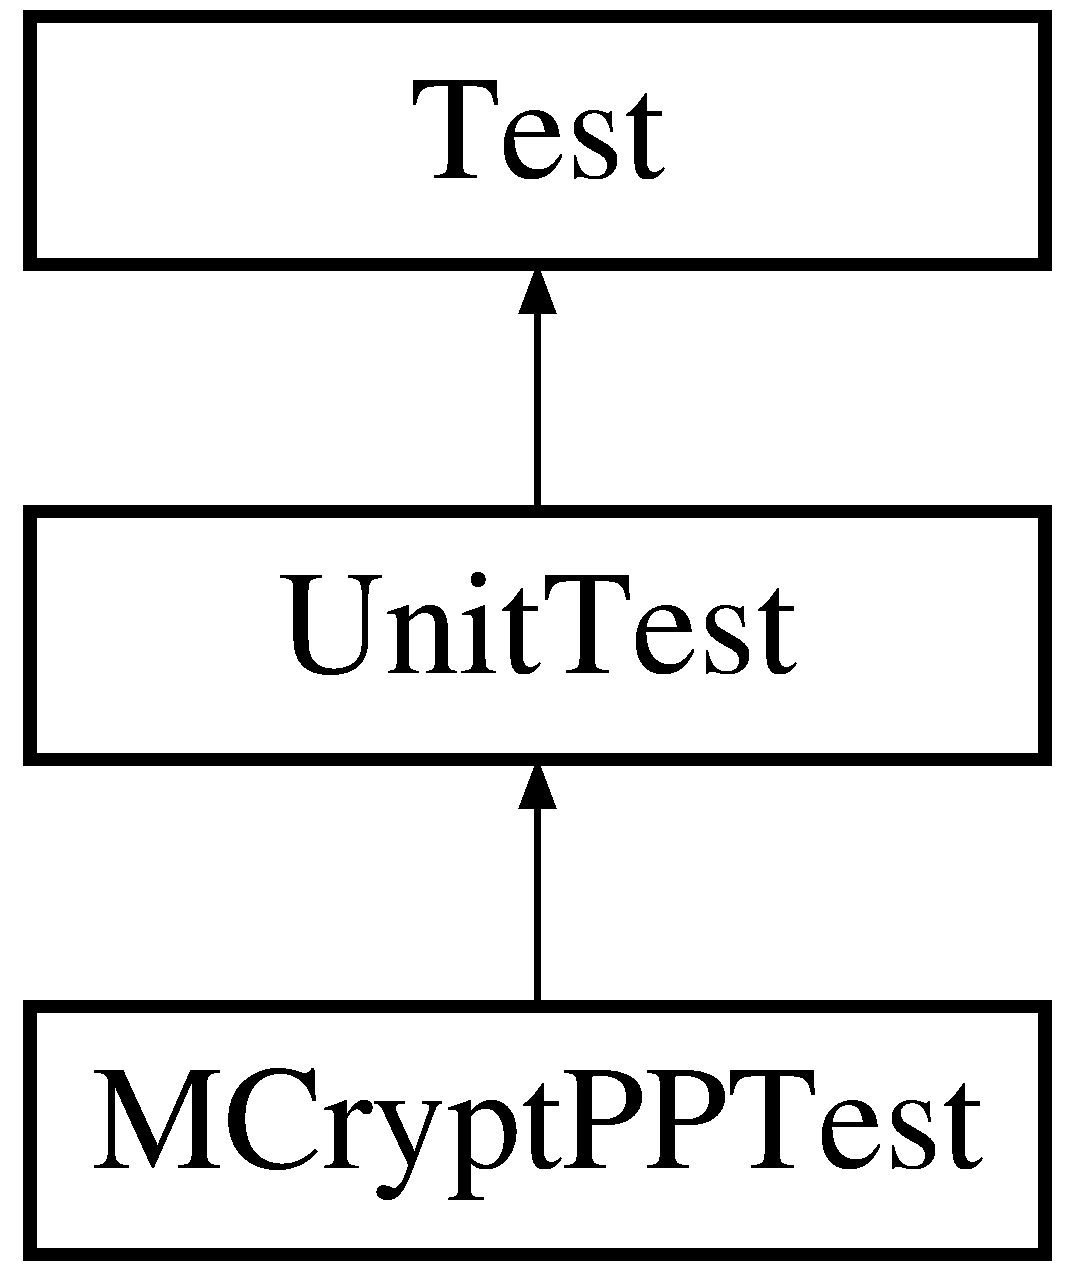
\includegraphics[height=3.000000cm]{classMCryptPPTest}
\end{center}
\end{figure}
\subsection*{Public Member Functions}
\begin{DoxyCompactItemize}
\item 
\textbf{ M\+Crypt\+P\+P\+Test} (\textbf{ Test\+Suite} $\ast$s)
\item 
void \textbf{ test\+Encryption} (void)
\item 
void \textbf{ test\+Decryption} (void)
\end{DoxyCompactItemize}
\subsection*{Private Member Functions}
\begin{DoxyCompactItemize}
\item 
bool \textbf{ generic\+Test\+Encryption} ()
\item 
bool \textbf{ generic\+Test\+Decryption} ()
\end{DoxyCompactItemize}
\subsection*{Additional Inherited Members}


\subsection{Constructor \& Destructor Documentation}
\mbox{\label{classMCryptPPTest_afe3dab17b61491ef222fac71386ad48e}} 
\index{M\+Crypt\+P\+P\+Test@{M\+Crypt\+P\+P\+Test}!M\+Crypt\+P\+P\+Test@{M\+Crypt\+P\+P\+Test}}
\index{M\+Crypt\+P\+P\+Test@{M\+Crypt\+P\+P\+Test}!M\+Crypt\+P\+P\+Test@{M\+Crypt\+P\+P\+Test}}
\subsubsection{M\+Crypt\+P\+P\+Test()}
{\footnotesize\ttfamily M\+Crypt\+P\+P\+Test\+::\+M\+Crypt\+P\+P\+Test (\begin{DoxyParamCaption}\item[{\textbf{ Test\+Suite} $\ast$}]{s }\end{DoxyParamCaption})}



\subsection{Member Function Documentation}
\mbox{\label{classMCryptPPTest_a7860564208a718dc1b6e5c3a3a4226c0}} 
\index{M\+Crypt\+P\+P\+Test@{M\+Crypt\+P\+P\+Test}!generic\+Test\+Decryption@{generic\+Test\+Decryption}}
\index{generic\+Test\+Decryption@{generic\+Test\+Decryption}!M\+Crypt\+P\+P\+Test@{M\+Crypt\+P\+P\+Test}}
\subsubsection{generic\+Test\+Decryption()}
{\footnotesize\ttfamily bool M\+Crypt\+P\+P\+Test\+::generic\+Test\+Decryption (\begin{DoxyParamCaption}{ }\end{DoxyParamCaption})\hspace{0.3cm}{\ttfamily [private]}}

\mbox{\label{classMCryptPPTest_a84a41a8cfe696d815d8312e2523ac034}} 
\index{M\+Crypt\+P\+P\+Test@{M\+Crypt\+P\+P\+Test}!generic\+Test\+Encryption@{generic\+Test\+Encryption}}
\index{generic\+Test\+Encryption@{generic\+Test\+Encryption}!M\+Crypt\+P\+P\+Test@{M\+Crypt\+P\+P\+Test}}
\subsubsection{generic\+Test\+Encryption()}
{\footnotesize\ttfamily bool M\+Crypt\+P\+P\+Test\+::generic\+Test\+Encryption (\begin{DoxyParamCaption}{ }\end{DoxyParamCaption})\hspace{0.3cm}{\ttfamily [private]}}

\mbox{\label{classMCryptPPTest_a3211d5f96b7a2ad4999d3a82bd88fa47}} 
\index{M\+Crypt\+P\+P\+Test@{M\+Crypt\+P\+P\+Test}!test\+Decryption@{test\+Decryption}}
\index{test\+Decryption@{test\+Decryption}!M\+Crypt\+P\+P\+Test@{M\+Crypt\+P\+P\+Test}}
\subsubsection{test\+Decryption()}
{\footnotesize\ttfamily void M\+Crypt\+P\+P\+Test\+::test\+Decryption (\begin{DoxyParamCaption}\item[{void}]{ }\end{DoxyParamCaption})}

\mbox{\label{classMCryptPPTest_a58ed41baeb9104e94e15a69a29b4ce6e}} 
\index{M\+Crypt\+P\+P\+Test@{M\+Crypt\+P\+P\+Test}!test\+Encryption@{test\+Encryption}}
\index{test\+Encryption@{test\+Encryption}!M\+Crypt\+P\+P\+Test@{M\+Crypt\+P\+P\+Test}}
\subsubsection{test\+Encryption()}
{\footnotesize\ttfamily void M\+Crypt\+P\+P\+Test\+::test\+Encryption (\begin{DoxyParamCaption}\item[{void}]{ }\end{DoxyParamCaption})}



The documentation for this class was generated from the following files\+:\begin{DoxyCompactItemize}
\item 
\textbf{ M\+Crypt\+P\+P\+Test.\+h}\item 
\textbf{ M\+Crypt\+P\+P\+Test.\+cc}\end{DoxyCompactItemize}

\section{Message Class Reference}
\label{classMessage}\index{Message@{Message}}


{\ttfamily \#include $<$msg.\+h$>$}

Inheritance diagram for Message\+:\begin{figure}[H]
\begin{center}
\leavevmode
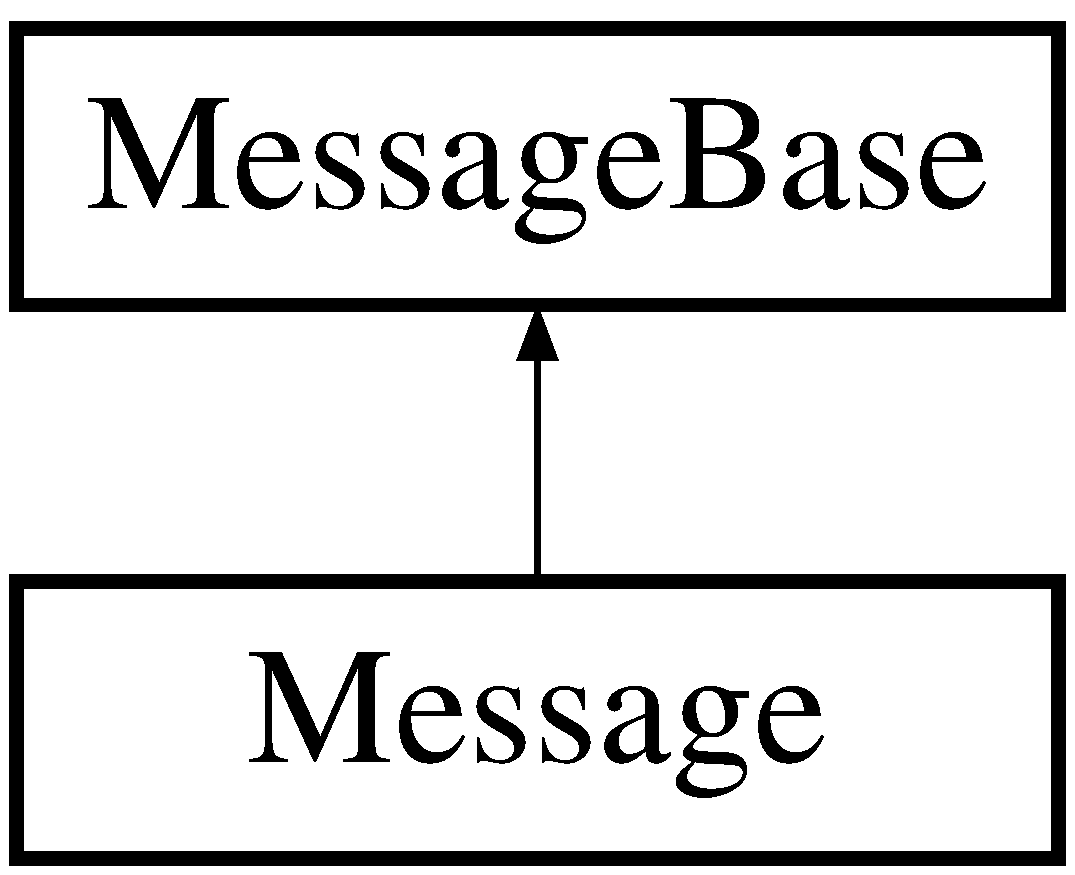
\includegraphics[height=2.000000cm]{classMessage}
\end{center}
\end{figure}
\subsection*{Public Member Functions}
\begin{DoxyCompactItemize}
\item 
\textbf{ Message} (void)
\item 
\textbf{ Message} (std\+::string msg)
\item 
\textbf{ Message} (const char $\ast$msgfmt,...)
\item 
void \textbf{ print\+Message} (void) const
\end{DoxyCompactItemize}
\subsection*{Additional Inherited Members}


\subsection{Constructor \& Destructor Documentation}
\mbox{\label{classMessage_a2ccdab4b2313d398d49f638a53f30103}} 
\index{Message@{Message}!Message@{Message}}
\index{Message@{Message}!Message@{Message}}
\subsubsection{Message()\hspace{0.1cm}{\footnotesize\ttfamily [1/3]}}
{\footnotesize\ttfamily Message\+::\+Message (\begin{DoxyParamCaption}\item[{void}]{ }\end{DoxyParamCaption})\hspace{0.3cm}{\ttfamily [inline]}}

\mbox{\label{classMessage_a4ce65abb94ebe52060af5d279f3e1944}} 
\index{Message@{Message}!Message@{Message}}
\index{Message@{Message}!Message@{Message}}
\subsubsection{Message()\hspace{0.1cm}{\footnotesize\ttfamily [2/3]}}
{\footnotesize\ttfamily Message\+::\+Message (\begin{DoxyParamCaption}\item[{std\+::string}]{msg }\end{DoxyParamCaption})\hspace{0.3cm}{\ttfamily [inline]}}

\mbox{\label{classMessage_a8dbca899c0164d0b5f9aca61bef113a1}} 
\index{Message@{Message}!Message@{Message}}
\index{Message@{Message}!Message@{Message}}
\subsubsection{Message()\hspace{0.1cm}{\footnotesize\ttfamily [3/3]}}
{\footnotesize\ttfamily Message\+::\+Message (\begin{DoxyParamCaption}\item[{const char $\ast$}]{msgfmt,  }\item[{}]{... }\end{DoxyParamCaption})}



\subsection{Member Function Documentation}
\mbox{\label{classMessage_a96dd19b80fb02907222585e33007e3a7}} 
\index{Message@{Message}!print\+Message@{print\+Message}}
\index{print\+Message@{print\+Message}!Message@{Message}}
\subsubsection{print\+Message()}
{\footnotesize\ttfamily void Message\+::print\+Message (\begin{DoxyParamCaption}\item[{void}]{ }\end{DoxyParamCaption}) const\hspace{0.3cm}{\ttfamily [virtual]}}



Implements \textbf{ Message\+Base} \doxyref{}{p.}{classMessageBase_a207178190da2bec546a972495cdf9bc6}.



The documentation for this class was generated from the following files\+:\begin{DoxyCompactItemize}
\item 
\textbf{ msg.\+h}\item 
\textbf{ msg.\+cc}\end{DoxyCompactItemize}

\section{Message\+Base Class Reference}
\label{classMessageBase}\index{Message\+Base@{Message\+Base}}


{\ttfamily \#include $<$msg.\+h$>$}

Inheritance diagram for Message\+Base\+:\begin{figure}[H]
\begin{center}
\leavevmode
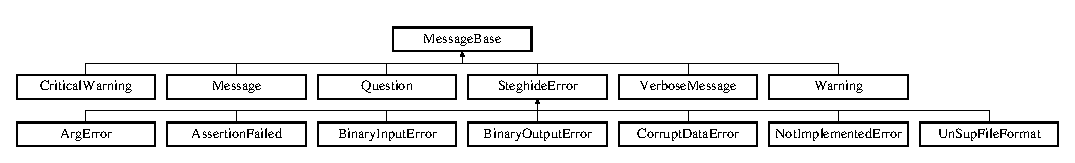
\includegraphics[height=1.739130cm]{classMessageBase}
\end{center}
\end{figure}
\subsection*{Public Member Functions}
\begin{DoxyCompactItemize}
\item 
\textbf{ Message\+Base} (void)
\item 
\textbf{ Message\+Base} (std\+::string msg)
\item 
\textbf{ Message\+Base} (const char $\ast$msgfmt,...)
\item 
virtual \textbf{ $\sim$\+Message\+Base} ()
\item 
const std\+::string \& \textbf{ get\+Message} (void) const
\item 
void \textbf{ set\+Message} (std\+::string msg)
\item 
void \textbf{ set\+Newline} (bool prnl)
\item 
const std\+::string \textbf{ get\+Newline} (void) const
\item 
void \textbf{ set\+Message} (const char $\ast$msgfmt,...)
\item 
virtual void \textbf{ print\+Message} (void) const =0
\end{DoxyCompactItemize}
\subsection*{Protected Member Functions}
\begin{DoxyCompactItemize}
\item 
std\+::string \textbf{ compose} (const char $\ast$msgfmt,...) const
\item 
std\+::string \textbf{ vcompose} (const char $\ast$msgfmt, va\+\_\+list ap) const
\end{DoxyCompactItemize}
\subsection*{Static Protected Attributes}
\begin{DoxyCompactItemize}
\item 
static const unsigned int \textbf{ Msg\+Max\+Size} = 512
\end{DoxyCompactItemize}
\subsection*{Private Attributes}
\begin{DoxyCompactItemize}
\item 
std\+::string \textbf{ Message}
\item 
bool \textbf{ Newline}
\end{DoxyCompactItemize}


\subsection{Constructor \& Destructor Documentation}
\mbox{\label{classMessageBase_acf6ea060e624f6db8babe88de299e230}} 
\index{Message\+Base@{Message\+Base}!Message\+Base@{Message\+Base}}
\index{Message\+Base@{Message\+Base}!Message\+Base@{Message\+Base}}
\subsubsection{Message\+Base()\hspace{0.1cm}{\footnotesize\ttfamily [1/3]}}
{\footnotesize\ttfamily Message\+Base\+::\+Message\+Base (\begin{DoxyParamCaption}\item[{void}]{ }\end{DoxyParamCaption})}

\mbox{\label{classMessageBase_a2e9dad473adc239134c60edb80de661e}} 
\index{Message\+Base@{Message\+Base}!Message\+Base@{Message\+Base}}
\index{Message\+Base@{Message\+Base}!Message\+Base@{Message\+Base}}
\subsubsection{Message\+Base()\hspace{0.1cm}{\footnotesize\ttfamily [2/3]}}
{\footnotesize\ttfamily Message\+Base\+::\+Message\+Base (\begin{DoxyParamCaption}\item[{std\+::string}]{msg }\end{DoxyParamCaption})}

\mbox{\label{classMessageBase_a55d2364790e0464914dbdecd14988032}} 
\index{Message\+Base@{Message\+Base}!Message\+Base@{Message\+Base}}
\index{Message\+Base@{Message\+Base}!Message\+Base@{Message\+Base}}
\subsubsection{Message\+Base()\hspace{0.1cm}{\footnotesize\ttfamily [3/3]}}
{\footnotesize\ttfamily Message\+Base\+::\+Message\+Base (\begin{DoxyParamCaption}\item[{const char $\ast$}]{msgfmt,  }\item[{}]{... }\end{DoxyParamCaption})}

\mbox{\label{classMessageBase_a9aeacbfb067feedb44738ee99f9d281c}} 
\index{Message\+Base@{Message\+Base}!````~Message\+Base@{$\sim$\+Message\+Base}}
\index{````~Message\+Base@{$\sim$\+Message\+Base}!Message\+Base@{Message\+Base}}
\subsubsection{$\sim$\+Message\+Base()}
{\footnotesize\ttfamily virtual Message\+Base\+::$\sim$\+Message\+Base (\begin{DoxyParamCaption}{ }\end{DoxyParamCaption})\hspace{0.3cm}{\ttfamily [inline]}, {\ttfamily [virtual]}}



\subsection{Member Function Documentation}
\mbox{\label{classMessageBase_a4e9a7c8408337eb3e2e0a934ac06ec7d}} 
\index{Message\+Base@{Message\+Base}!compose@{compose}}
\index{compose@{compose}!Message\+Base@{Message\+Base}}
\subsubsection{compose()}
{\footnotesize\ttfamily std\+::string Message\+Base\+::compose (\begin{DoxyParamCaption}\item[{const char $\ast$}]{msgfmt,  }\item[{}]{... }\end{DoxyParamCaption}) const\hspace{0.3cm}{\ttfamily [protected]}}

\mbox{\label{classMessageBase_abf3214aff1175a0219ca2f9cb60dfb1a}} 
\index{Message\+Base@{Message\+Base}!get\+Message@{get\+Message}}
\index{get\+Message@{get\+Message}!Message\+Base@{Message\+Base}}
\subsubsection{get\+Message()}
{\footnotesize\ttfamily const std\+::string\& Message\+Base\+::get\+Message (\begin{DoxyParamCaption}\item[{void}]{ }\end{DoxyParamCaption}) const\hspace{0.3cm}{\ttfamily [inline]}}

\mbox{\label{classMessageBase_a4f48f8273be5cc7c3de17c42fad58349}} 
\index{Message\+Base@{Message\+Base}!get\+Newline@{get\+Newline}}
\index{get\+Newline@{get\+Newline}!Message\+Base@{Message\+Base}}
\subsubsection{get\+Newline()}
{\footnotesize\ttfamily const std\+::string Message\+Base\+::get\+Newline (\begin{DoxyParamCaption}\item[{void}]{ }\end{DoxyParamCaption}) const\hspace{0.3cm}{\ttfamily [inline]}}

return either \char`\"{}\textbackslash{}n\char`\"{} or \char`\"{}\char`\"{} depending on wether this message should be followed by a newline or not \mbox{\label{classMessageBase_a207178190da2bec546a972495cdf9bc6}} 
\index{Message\+Base@{Message\+Base}!print\+Message@{print\+Message}}
\index{print\+Message@{print\+Message}!Message\+Base@{Message\+Base}}
\subsubsection{print\+Message()}
{\footnotesize\ttfamily virtual void Message\+Base\+::print\+Message (\begin{DoxyParamCaption}\item[{void}]{ }\end{DoxyParamCaption}) const\hspace{0.3cm}{\ttfamily [pure virtual]}}



Implemented in \textbf{ Question} \doxyref{}{p.}{classQuestion_a5b0fe8561addc6710984b02b34cfe68c}, \textbf{ Critical\+Warning} \doxyref{}{p.}{classCriticalWarning_af92d1c346a1a0ec2a150a46d90afe2f5}, \textbf{ Warning} \doxyref{}{p.}{classWarning_af91afcff6919bda9f7c8bec584cbc68c}, \textbf{ Corrupt\+Data\+Error} \doxyref{}{p.}{classCorruptDataError_a345998f46c50877c96d40c1d349f2a1a}, \textbf{ Verbose\+Message} \doxyref{}{p.}{classVerboseMessage_ac54162e30aec66d4fb07d99eadfd8b52}, \textbf{ Not\+Implemented\+Error} \doxyref{}{p.}{classNotImplementedError_abbe96cc33b89076043f8f71fde80a0cd}, \textbf{ Message} \doxyref{}{p.}{classMessage_a96dd19b80fb02907222585e33007e3a7}, \textbf{ Arg\+Error} \doxyref{}{p.}{classArgError_a45233b131442b1af57c8278485856a83}, \textbf{ Steghide\+Error} \doxyref{}{p.}{classSteghideError_a22d688da944706920f51159ebd0076d9}, and \textbf{ Assertion\+Failed} \doxyref{}{p.}{classAssertionFailed_acab14a3cc730015f7c8c76a17d0b347c}.

\mbox{\label{classMessageBase_a30b3927e0f2eb7c47fa14f67af027397}} 
\index{Message\+Base@{Message\+Base}!set\+Message@{set\+Message}}
\index{set\+Message@{set\+Message}!Message\+Base@{Message\+Base}}
\subsubsection{set\+Message()\hspace{0.1cm}{\footnotesize\ttfamily [1/2]}}
{\footnotesize\ttfamily void Message\+Base\+::set\+Message (\begin{DoxyParamCaption}\item[{std\+::string}]{msg }\end{DoxyParamCaption})\hspace{0.3cm}{\ttfamily [inline]}}

\mbox{\label{classMessageBase_ab927341ddd9c9cb558a544e15bfc356b}} 
\index{Message\+Base@{Message\+Base}!set\+Message@{set\+Message}}
\index{set\+Message@{set\+Message}!Message\+Base@{Message\+Base}}
\subsubsection{set\+Message()\hspace{0.1cm}{\footnotesize\ttfamily [2/2]}}
{\footnotesize\ttfamily void Message\+Base\+::set\+Message (\begin{DoxyParamCaption}\item[{const char $\ast$}]{msgfmt,  }\item[{}]{... }\end{DoxyParamCaption})}

\mbox{\label{classMessageBase_a46e7f5b7693a4dcce4a20c7b29fb0c5a}} 
\index{Message\+Base@{Message\+Base}!set\+Newline@{set\+Newline}}
\index{set\+Newline@{set\+Newline}!Message\+Base@{Message\+Base}}
\subsubsection{set\+Newline()}
{\footnotesize\ttfamily void Message\+Base\+::set\+Newline (\begin{DoxyParamCaption}\item[{bool}]{prnl }\end{DoxyParamCaption})\hspace{0.3cm}{\ttfamily [inline]}}

toggle newline printing on/off 
\begin{DoxyParams}{Parameters}
{\em prnl} & wether to print a newline character after the message \\
\hline
\end{DoxyParams}
\mbox{\label{classMessageBase_a8394206583995f6fbfe858d656968490}} 
\index{Message\+Base@{Message\+Base}!vcompose@{vcompose}}
\index{vcompose@{vcompose}!Message\+Base@{Message\+Base}}
\subsubsection{vcompose()}
{\footnotesize\ttfamily std\+::string Message\+Base\+::vcompose (\begin{DoxyParamCaption}\item[{const char $\ast$}]{msgfmt,  }\item[{va\+\_\+list}]{ap }\end{DoxyParamCaption}) const\hspace{0.3cm}{\ttfamily [protected]}}



\subsection{Member Data Documentation}
\mbox{\label{classMessageBase_a9383dfdf1b15fc5ec1bfc3b00619bb47}} 
\index{Message\+Base@{Message\+Base}!Message@{Message}}
\index{Message@{Message}!Message\+Base@{Message\+Base}}
\subsubsection{Message}
{\footnotesize\ttfamily std\+::string Message\+Base\+::\+Message\hspace{0.3cm}{\ttfamily [private]}}

\mbox{\label{classMessageBase_af16e9e59496a1277b4baa08828c9f388}} 
\index{Message\+Base@{Message\+Base}!Msg\+Max\+Size@{Msg\+Max\+Size}}
\index{Msg\+Max\+Size@{Msg\+Max\+Size}!Message\+Base@{Message\+Base}}
\subsubsection{Msg\+Max\+Size}
{\footnotesize\ttfamily const unsigned int Message\+Base\+::\+Msg\+Max\+Size = 512\hspace{0.3cm}{\ttfamily [static]}, {\ttfamily [protected]}}

\mbox{\label{classMessageBase_a926ed952613f951d8f17e14c340614d3}} 
\index{Message\+Base@{Message\+Base}!Newline@{Newline}}
\index{Newline@{Newline}!Message\+Base@{Message\+Base}}
\subsubsection{Newline}
{\footnotesize\ttfamily bool Message\+Base\+::\+Newline\hspace{0.3cm}{\ttfamily [private]}}



The documentation for this class was generated from the following files\+:\begin{DoxyCompactItemize}
\item 
\textbf{ msg.\+h}\item 
\textbf{ msg.\+cc}\end{DoxyCompactItemize}

\section{M\+Hash\+Key\+Gen Class Reference}
\label{classMHashKeyGen}\index{M\+Hash\+Key\+Gen@{M\+Hash\+Key\+Gen}}


{\ttfamily \#include $<$M\+Hash\+Key\+Gen.\+h$>$}

\subsection*{Public Member Functions}
\begin{DoxyCompactItemize}
\item 
\textbf{ M\+Hash\+Key\+Gen} (void)
\item 
\textbf{ M\+Hash\+Key\+Gen} (keygenid kgalgo, hashid halgo, unsigned int keysize)
\item 
\textbf{ $\sim$\+M\+Hash\+Key\+Gen} (void)
\item 
void \textbf{ set\+Key\+Size} (unsigned int \textbf{ Key\+Size})
\item 
void \textbf{ set\+Key\+Gen\+Algorithm} (keygenid algo)
\item 
void \textbf{ set\+Hash\+Algorithm} (hashid hashalgo)
\item 
void \textbf{ set\+Hash\+Algorithms} (std\+::vector$<$ hashid $>$ hashalgos)
\item 
void \textbf{ set\+Salt} (std\+::vector$<$ unsigned char $>$ salt)
\item 
std\+::vector$<$ unsigned char $>$ \textbf{ create\+Key} (std\+::string password)
\end{DoxyCompactItemize}
\subsection*{Private Member Functions}
\begin{DoxyCompactItemize}
\item 
void $\ast$ \textbf{ s\+\_\+malloc} (size\+\_\+t size)
\end{DoxyCompactItemize}
\subsection*{Private Attributes}
\begin{DoxyCompactItemize}
\item 
bool \textbf{ ready}
\item 
keygenid \textbf{ Algorithm}
\item 
K\+E\+Y\+G\+EN \textbf{ Algorithm\+Data}
\item 
unsigned int \textbf{ Key\+Size}
\end{DoxyCompactItemize}


\subsection{Constructor \& Destructor Documentation}
\mbox{\label{classMHashKeyGen_a1cffb83fdf21b8300eac6e162a40dfee}} 
\index{M\+Hash\+Key\+Gen@{M\+Hash\+Key\+Gen}!M\+Hash\+Key\+Gen@{M\+Hash\+Key\+Gen}}
\index{M\+Hash\+Key\+Gen@{M\+Hash\+Key\+Gen}!M\+Hash\+Key\+Gen@{M\+Hash\+Key\+Gen}}
\subsubsection{M\+Hash\+Key\+Gen()\hspace{0.1cm}{\footnotesize\ttfamily [1/2]}}
{\footnotesize\ttfamily M\+Hash\+Key\+Gen\+::\+M\+Hash\+Key\+Gen (\begin{DoxyParamCaption}\item[{void}]{ }\end{DoxyParamCaption})}

\mbox{\label{classMHashKeyGen_ae871e6bdee1a294aa6afa0730fd0d1aa}} 
\index{M\+Hash\+Key\+Gen@{M\+Hash\+Key\+Gen}!M\+Hash\+Key\+Gen@{M\+Hash\+Key\+Gen}}
\index{M\+Hash\+Key\+Gen@{M\+Hash\+Key\+Gen}!M\+Hash\+Key\+Gen@{M\+Hash\+Key\+Gen}}
\subsubsection{M\+Hash\+Key\+Gen()\hspace{0.1cm}{\footnotesize\ttfamily [2/2]}}
{\footnotesize\ttfamily M\+Hash\+Key\+Gen\+::\+M\+Hash\+Key\+Gen (\begin{DoxyParamCaption}\item[{keygenid}]{kgalgo,  }\item[{hashid}]{halgo,  }\item[{unsigned int}]{keysize }\end{DoxyParamCaption})}

\mbox{\label{classMHashKeyGen_ac84419b92def320f8c7f3fdd6a82838c}} 
\index{M\+Hash\+Key\+Gen@{M\+Hash\+Key\+Gen}!````~M\+Hash\+Key\+Gen@{$\sim$\+M\+Hash\+Key\+Gen}}
\index{````~M\+Hash\+Key\+Gen@{$\sim$\+M\+Hash\+Key\+Gen}!M\+Hash\+Key\+Gen@{M\+Hash\+Key\+Gen}}
\subsubsection{$\sim$\+M\+Hash\+Key\+Gen()}
{\footnotesize\ttfamily M\+Hash\+Key\+Gen\+::$\sim$\+M\+Hash\+Key\+Gen (\begin{DoxyParamCaption}\item[{void}]{ }\end{DoxyParamCaption})}



\subsection{Member Function Documentation}
\mbox{\label{classMHashKeyGen_a94021d906060002d1d4c2ff7c141389d}} 
\index{M\+Hash\+Key\+Gen@{M\+Hash\+Key\+Gen}!create\+Key@{create\+Key}}
\index{create\+Key@{create\+Key}!M\+Hash\+Key\+Gen@{M\+Hash\+Key\+Gen}}
\subsubsection{create\+Key()}
{\footnotesize\ttfamily std\+::vector$<$ unsigned char $>$ M\+Hash\+Key\+Gen\+::create\+Key (\begin{DoxyParamCaption}\item[{std\+::string}]{password }\end{DoxyParamCaption})}

\mbox{\label{classMHashKeyGen_aa64a9326a3c3fb931d535afd95afb738}} 
\index{M\+Hash\+Key\+Gen@{M\+Hash\+Key\+Gen}!s\+\_\+malloc@{s\+\_\+malloc}}
\index{s\+\_\+malloc@{s\+\_\+malloc}!M\+Hash\+Key\+Gen@{M\+Hash\+Key\+Gen}}
\subsubsection{s\+\_\+malloc()}
{\footnotesize\ttfamily void $\ast$ M\+Hash\+Key\+Gen\+::s\+\_\+malloc (\begin{DoxyParamCaption}\item[{size\+\_\+t}]{size }\end{DoxyParamCaption})\hspace{0.3cm}{\ttfamily [private]}}

\mbox{\label{classMHashKeyGen_a8c274ba1b37bb5075e9f122ce97d6fa9}} 
\index{M\+Hash\+Key\+Gen@{M\+Hash\+Key\+Gen}!set\+Hash\+Algorithm@{set\+Hash\+Algorithm}}
\index{set\+Hash\+Algorithm@{set\+Hash\+Algorithm}!M\+Hash\+Key\+Gen@{M\+Hash\+Key\+Gen}}
\subsubsection{set\+Hash\+Algorithm()}
{\footnotesize\ttfamily void M\+Hash\+Key\+Gen\+::set\+Hash\+Algorithm (\begin{DoxyParamCaption}\item[{hashid}]{hashalgo }\end{DoxyParamCaption})}

\mbox{\label{classMHashKeyGen_a24fb66cb5aa7c5120ca8b65667435c5b}} 
\index{M\+Hash\+Key\+Gen@{M\+Hash\+Key\+Gen}!set\+Hash\+Algorithms@{set\+Hash\+Algorithms}}
\index{set\+Hash\+Algorithms@{set\+Hash\+Algorithms}!M\+Hash\+Key\+Gen@{M\+Hash\+Key\+Gen}}
\subsubsection{set\+Hash\+Algorithms()}
{\footnotesize\ttfamily void M\+Hash\+Key\+Gen\+::set\+Hash\+Algorithms (\begin{DoxyParamCaption}\item[{std\+::vector$<$ hashid $>$}]{hashalgos }\end{DoxyParamCaption})}

\mbox{\label{classMHashKeyGen_a793284ce053ce3ea4c81a53d2c8d5f3a}} 
\index{M\+Hash\+Key\+Gen@{M\+Hash\+Key\+Gen}!set\+Key\+Gen\+Algorithm@{set\+Key\+Gen\+Algorithm}}
\index{set\+Key\+Gen\+Algorithm@{set\+Key\+Gen\+Algorithm}!M\+Hash\+Key\+Gen@{M\+Hash\+Key\+Gen}}
\subsubsection{set\+Key\+Gen\+Algorithm()}
{\footnotesize\ttfamily void M\+Hash\+Key\+Gen\+::set\+Key\+Gen\+Algorithm (\begin{DoxyParamCaption}\item[{keygenid}]{algo }\end{DoxyParamCaption})}

\mbox{\label{classMHashKeyGen_afb604d40cffc15747e3e22cf145537bf}} 
\index{M\+Hash\+Key\+Gen@{M\+Hash\+Key\+Gen}!set\+Key\+Size@{set\+Key\+Size}}
\index{set\+Key\+Size@{set\+Key\+Size}!M\+Hash\+Key\+Gen@{M\+Hash\+Key\+Gen}}
\subsubsection{set\+Key\+Size()}
{\footnotesize\ttfamily void M\+Hash\+Key\+Gen\+::set\+Key\+Size (\begin{DoxyParamCaption}\item[{unsigned int}]{Key\+Size }\end{DoxyParamCaption})}

\mbox{\label{classMHashKeyGen_ade5e590e9a7fe3e880a548d5a1f527bd}} 
\index{M\+Hash\+Key\+Gen@{M\+Hash\+Key\+Gen}!set\+Salt@{set\+Salt}}
\index{set\+Salt@{set\+Salt}!M\+Hash\+Key\+Gen@{M\+Hash\+Key\+Gen}}
\subsubsection{set\+Salt()}
{\footnotesize\ttfamily void M\+Hash\+Key\+Gen\+::set\+Salt (\begin{DoxyParamCaption}\item[{std\+::vector$<$ unsigned char $>$}]{salt }\end{DoxyParamCaption})}



\subsection{Member Data Documentation}
\mbox{\label{classMHashKeyGen_a02555544aabc2ee67796b29b4c2e2fa2}} 
\index{M\+Hash\+Key\+Gen@{M\+Hash\+Key\+Gen}!Algorithm@{Algorithm}}
\index{Algorithm@{Algorithm}!M\+Hash\+Key\+Gen@{M\+Hash\+Key\+Gen}}
\subsubsection{Algorithm}
{\footnotesize\ttfamily keygenid M\+Hash\+Key\+Gen\+::\+Algorithm\hspace{0.3cm}{\ttfamily [private]}}

\mbox{\label{classMHashKeyGen_a2983042aa752b477e867ae694c44e020}} 
\index{M\+Hash\+Key\+Gen@{M\+Hash\+Key\+Gen}!Algorithm\+Data@{Algorithm\+Data}}
\index{Algorithm\+Data@{Algorithm\+Data}!M\+Hash\+Key\+Gen@{M\+Hash\+Key\+Gen}}
\subsubsection{Algorithm\+Data}
{\footnotesize\ttfamily K\+E\+Y\+G\+EN M\+Hash\+Key\+Gen\+::\+Algorithm\+Data\hspace{0.3cm}{\ttfamily [private]}}

\mbox{\label{classMHashKeyGen_a339c55fa387f746241004036c7119524}} 
\index{M\+Hash\+Key\+Gen@{M\+Hash\+Key\+Gen}!Key\+Size@{Key\+Size}}
\index{Key\+Size@{Key\+Size}!M\+Hash\+Key\+Gen@{M\+Hash\+Key\+Gen}}
\subsubsection{Key\+Size}
{\footnotesize\ttfamily unsigned int M\+Hash\+Key\+Gen\+::\+Key\+Size\hspace{0.3cm}{\ttfamily [private]}}

\mbox{\label{classMHashKeyGen_ab6b00edfe8982171fb991ef527256bde}} 
\index{M\+Hash\+Key\+Gen@{M\+Hash\+Key\+Gen}!ready@{ready}}
\index{ready@{ready}!M\+Hash\+Key\+Gen@{M\+Hash\+Key\+Gen}}
\subsubsection{ready}
{\footnotesize\ttfamily bool M\+Hash\+Key\+Gen\+::ready\hspace{0.3cm}{\ttfamily [private]}}



The documentation for this class was generated from the following files\+:\begin{DoxyCompactItemize}
\item 
\textbf{ M\+Hash\+Key\+Gen.\+h}\item 
\textbf{ M\+Hash\+Key\+Gen.\+cc}\end{DoxyCompactItemize}

\section{M\+Hash\+Key\+Gen\+Test Class Reference}
\label{classMHashKeyGenTest}\index{M\+Hash\+Key\+Gen\+Test@{M\+Hash\+Key\+Gen\+Test}}


{\ttfamily \#include $<$M\+Hash\+Key\+Gen\+Test.\+h$>$}

Inheritance diagram for M\+Hash\+Key\+Gen\+Test\+:\begin{figure}[H]
\begin{center}
\leavevmode
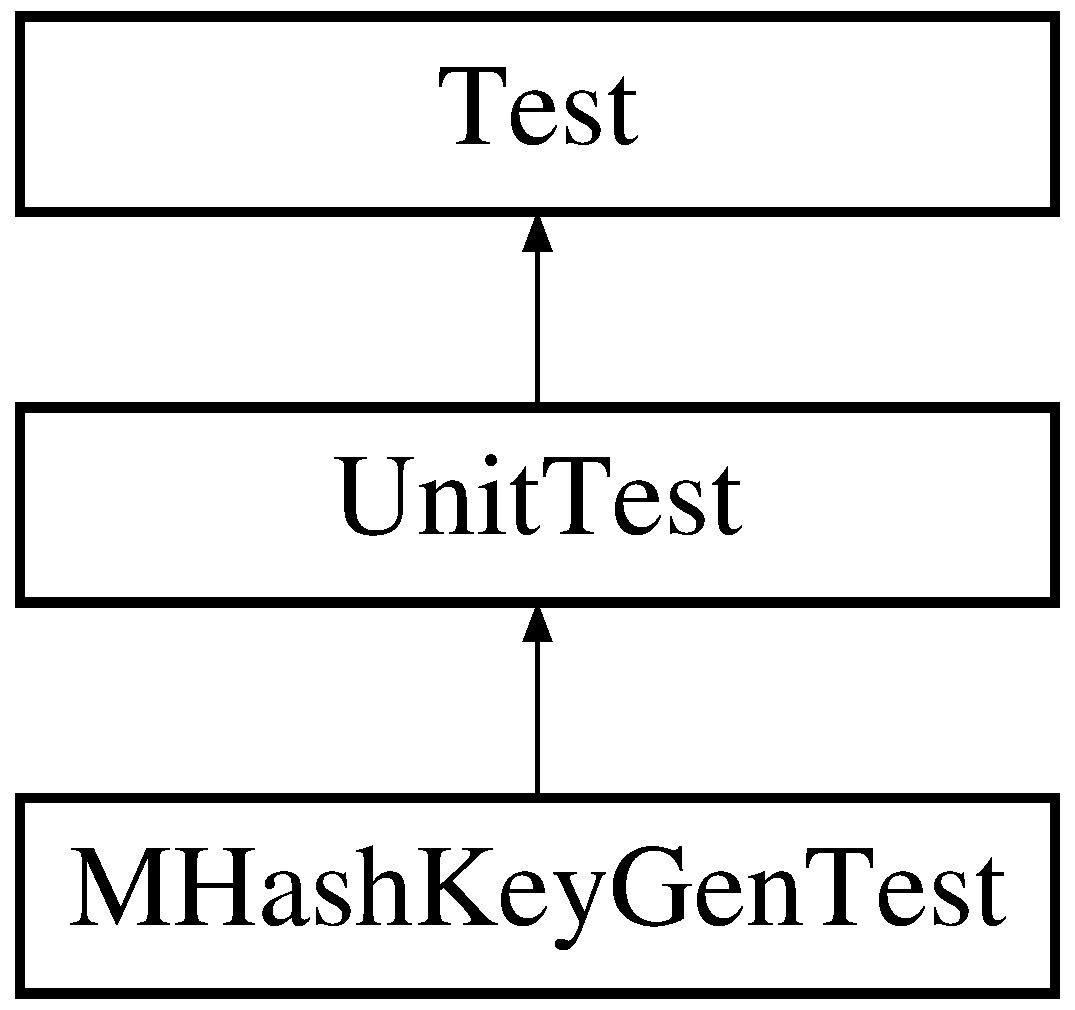
\includegraphics[height=3.000000cm]{classMHashKeyGenTest}
\end{center}
\end{figure}
\subsection*{Public Member Functions}
\begin{DoxyCompactItemize}
\item 
\textbf{ M\+Hash\+Key\+Gen\+Test} (\textbf{ Test\+Suite} $\ast$s)
\end{DoxyCompactItemize}
\subsection*{Additional Inherited Members}


\subsection{Constructor \& Destructor Documentation}
\mbox{\label{classMHashKeyGenTest_a723f3c8406cb1a2b9093eab0a2156c16}} 
\index{M\+Hash\+Key\+Gen\+Test@{M\+Hash\+Key\+Gen\+Test}!M\+Hash\+Key\+Gen\+Test@{M\+Hash\+Key\+Gen\+Test}}
\index{M\+Hash\+Key\+Gen\+Test@{M\+Hash\+Key\+Gen\+Test}!M\+Hash\+Key\+Gen\+Test@{M\+Hash\+Key\+Gen\+Test}}
\subsubsection{M\+Hash\+Key\+Gen\+Test()}
{\footnotesize\ttfamily M\+Hash\+Key\+Gen\+Test\+::\+M\+Hash\+Key\+Gen\+Test (\begin{DoxyParamCaption}\item[{\textbf{ Test\+Suite} $\ast$}]{s }\end{DoxyParamCaption})}



The documentation for this class was generated from the following files\+:\begin{DoxyCompactItemize}
\item 
\textbf{ M\+Hash\+Key\+Gen\+Test.\+h}\item 
\textbf{ M\+Hash\+Key\+Gen\+Test.\+cc}\end{DoxyCompactItemize}

\section{M\+Hash\+PP Class Reference}
\label{classMHashPP}\index{M\+Hash\+PP@{M\+Hash\+PP}}


{\ttfamily \#include $<$M\+Hash\+P\+P.\+h$>$}

\subsection*{Public Types}
\begin{DoxyCompactItemize}
\item 
enum \textbf{ Command} \{ \textbf{ endhash}
 \}
\end{DoxyCompactItemize}
\subsection*{Public Member Functions}
\begin{DoxyCompactItemize}
\item 
\textbf{ M\+Hash\+PP} (void)
\item 
\textbf{ M\+Hash\+PP} (hashid a)
\item 
void \textbf{ init} (hashid a)
\item 
const std\+::vector$<$ \textbf{ B\+Y\+TE} $>$ \& \textbf{ end} (void)
\item 
\textbf{ M\+Hash\+PP} \& \textbf{ operator$<$$<$} (std\+::string v)
\item 
\textbf{ M\+Hash\+PP} \& \textbf{ operator$<$$<$} (\textbf{ Bit\+String} v)
\item 
\textbf{ M\+Hash\+PP} \& \textbf{ operator$<$$<$} (\textbf{ B\+Y\+TE} v)
\item 
\textbf{ M\+Hash\+PP} \& \textbf{ operator$<$$<$} (\textbf{ Command} c)
\item 
\textbf{ Bit\+String} \textbf{ get\+Hash\+Bits} (void)
\item 
const std\+::vector$<$ \textbf{ B\+Y\+TE} $>$ \& \textbf{ get\+Hash\+Bytes} (void)
\item 
unsigned int \textbf{ get\+Hash\+Size} (void)
\end{DoxyCompactItemize}
\subsection*{Private Member Functions}
\begin{DoxyCompactItemize}
\item 
std\+::string \textbf{ get\+Algorithm\+Name} (void)
\end{DoxyCompactItemize}
\subsection*{Static Private Member Functions}
\begin{DoxyCompactItemize}
\item 
static std\+::string \textbf{ get\+Algorithm\+Name} (hashid id)
\end{DoxyCompactItemize}
\subsection*{Private Attributes}
\begin{DoxyCompactItemize}
\item 
bool \textbf{ hashing}
\begin{DoxyCompactList}\small\item\em true iff HashD contains a legal hash descriptor and data can be passed via $<$$<$ \end{DoxyCompactList}\item 
M\+H\+A\+SH \textbf{ HashD}
\item 
bool \textbf{ Hash\+Bytes\+Valid}
\begin{DoxyCompactList}\small\item\em true iff Hash\+Bytes contains a valid hash value \end{DoxyCompactList}\item 
std\+::vector$<$ \textbf{ B\+Y\+TE} $>$ \textbf{ Hash\+Bytes}
\end{DoxyCompactItemize}


\subsection{Member Enumeration Documentation}
\mbox{\label{classMHashPP_ac7390fc319fa6359e869ec9488d633ec}} 
\index{M\+Hash\+PP@{M\+Hash\+PP}!Command@{Command}}
\index{Command@{Command}!M\+Hash\+PP@{M\+Hash\+PP}}
\subsubsection{Command}
{\footnotesize\ttfamily enum \textbf{ M\+Hash\+P\+P\+::\+Command}}

\begin{DoxyEnumFields}{Enumerator}
\raisebox{\heightof{T}}[0pt][0pt]{\index{endhash@{endhash}!M\+Hash\+PP@{M\+Hash\+PP}}\index{M\+Hash\+PP@{M\+Hash\+PP}!endhash@{endhash}}}\mbox{\label{classMHashPP_ac7390fc319fa6359e869ec9488d633eca3b9758f6c85df34357793d9110dd101f}} 
endhash&\\
\hline

\end{DoxyEnumFields}


\subsection{Constructor \& Destructor Documentation}
\mbox{\label{classMHashPP_a81d66380d1300a707d412089b7fa03a2}} 
\index{M\+Hash\+PP@{M\+Hash\+PP}!M\+Hash\+PP@{M\+Hash\+PP}}
\index{M\+Hash\+PP@{M\+Hash\+PP}!M\+Hash\+PP@{M\+Hash\+PP}}
\subsubsection{M\+Hash\+P\+P()\hspace{0.1cm}{\footnotesize\ttfamily [1/2]}}
{\footnotesize\ttfamily M\+Hash\+P\+P\+::\+M\+Hash\+PP (\begin{DoxyParamCaption}\item[{void}]{ }\end{DoxyParamCaption})}

\mbox{\label{classMHashPP_a5aa71b96476ef66d40abeed70e6ded19}} 
\index{M\+Hash\+PP@{M\+Hash\+PP}!M\+Hash\+PP@{M\+Hash\+PP}}
\index{M\+Hash\+PP@{M\+Hash\+PP}!M\+Hash\+PP@{M\+Hash\+PP}}
\subsubsection{M\+Hash\+P\+P()\hspace{0.1cm}{\footnotesize\ttfamily [2/2]}}
{\footnotesize\ttfamily M\+Hash\+P\+P\+::\+M\+Hash\+PP (\begin{DoxyParamCaption}\item[{hashid}]{a }\end{DoxyParamCaption})}



\subsection{Member Function Documentation}
\mbox{\label{classMHashPP_a4478a5fadf4955519a3249bec76caf1e}} 
\index{M\+Hash\+PP@{M\+Hash\+PP}!end@{end}}
\index{end@{end}!M\+Hash\+PP@{M\+Hash\+PP}}
\subsubsection{end()}
{\footnotesize\ttfamily const std\+::vector$<$ \textbf{ B\+Y\+TE} $>$ \& M\+Hash\+P\+P\+::end (\begin{DoxyParamCaption}\item[{void}]{ }\end{DoxyParamCaption})}

\mbox{\label{classMHashPP_ab9a986263a0ef41639a2735aa8bb09b3}} 
\index{M\+Hash\+PP@{M\+Hash\+PP}!get\+Algorithm\+Name@{get\+Algorithm\+Name}}
\index{get\+Algorithm\+Name@{get\+Algorithm\+Name}!M\+Hash\+PP@{M\+Hash\+PP}}
\subsubsection{get\+Algorithm\+Name()\hspace{0.1cm}{\footnotesize\ttfamily [1/2]}}
{\footnotesize\ttfamily std\+::string M\+Hash\+P\+P\+::get\+Algorithm\+Name (\begin{DoxyParamCaption}\item[{void}]{ }\end{DoxyParamCaption})\hspace{0.3cm}{\ttfamily [private]}}

\mbox{\label{classMHashPP_a9d7887a9f3ed507a075be49a10d56fbb}} 
\index{M\+Hash\+PP@{M\+Hash\+PP}!get\+Algorithm\+Name@{get\+Algorithm\+Name}}
\index{get\+Algorithm\+Name@{get\+Algorithm\+Name}!M\+Hash\+PP@{M\+Hash\+PP}}
\subsubsection{get\+Algorithm\+Name()\hspace{0.1cm}{\footnotesize\ttfamily [2/2]}}
{\footnotesize\ttfamily std\+::string M\+Hash\+P\+P\+::get\+Algorithm\+Name (\begin{DoxyParamCaption}\item[{hashid}]{id }\end{DoxyParamCaption})\hspace{0.3cm}{\ttfamily [static]}, {\ttfamily [private]}}

\mbox{\label{classMHashPP_ac9a617262342f96190b12b5f8973d8ee}} 
\index{M\+Hash\+PP@{M\+Hash\+PP}!get\+Hash\+Bits@{get\+Hash\+Bits}}
\index{get\+Hash\+Bits@{get\+Hash\+Bits}!M\+Hash\+PP@{M\+Hash\+PP}}
\subsubsection{get\+Hash\+Bits()}
{\footnotesize\ttfamily \textbf{ Bit\+String} M\+Hash\+P\+P\+::get\+Hash\+Bits (\begin{DoxyParamCaption}\item[{void}]{ }\end{DoxyParamCaption})}

get the hash bits \begin{DoxyReturn}{Returns}
the hash value of the data that has been passed via $<$$<$ 
\end{DoxyReturn}
\mbox{\label{classMHashPP_a386c7cfc3d953d4a3c4a20a867c508aa}} 
\index{M\+Hash\+PP@{M\+Hash\+PP}!get\+Hash\+Bytes@{get\+Hash\+Bytes}}
\index{get\+Hash\+Bytes@{get\+Hash\+Bytes}!M\+Hash\+PP@{M\+Hash\+PP}}
\subsubsection{get\+Hash\+Bytes()}
{\footnotesize\ttfamily const std\+::vector$<$ \textbf{ B\+Y\+TE} $>$ \& M\+Hash\+P\+P\+::get\+Hash\+Bytes (\begin{DoxyParamCaption}\item[{void}]{ }\end{DoxyParamCaption})}

\mbox{\label{classMHashPP_a844895b753aaff388be34cdb5332687f}} 
\index{M\+Hash\+PP@{M\+Hash\+PP}!get\+Hash\+Size@{get\+Hash\+Size}}
\index{get\+Hash\+Size@{get\+Hash\+Size}!M\+Hash\+PP@{M\+Hash\+PP}}
\subsubsection{get\+Hash\+Size()}
{\footnotesize\ttfamily unsigned int M\+Hash\+P\+P\+::get\+Hash\+Size (\begin{DoxyParamCaption}\item[{void}]{ }\end{DoxyParamCaption})}

get the hash size \begin{DoxyReturn}{Returns}
the size of the value returned by get\+Hash\+Bits in bytes 
\end{DoxyReturn}
\mbox{\label{classMHashPP_af65d7afba20d0e7bf17c3b0021994385}} 
\index{M\+Hash\+PP@{M\+Hash\+PP}!init@{init}}
\index{init@{init}!M\+Hash\+PP@{M\+Hash\+PP}}
\subsubsection{init()}
{\footnotesize\ttfamily void M\+Hash\+P\+P\+::init (\begin{DoxyParamCaption}\item[{hashid}]{a }\end{DoxyParamCaption})}

\mbox{\label{classMHashPP_adcd3d311e973d71d630a8eca38175141}} 
\index{M\+Hash\+PP@{M\+Hash\+PP}!operator$<$$<$@{operator$<$$<$}}
\index{operator$<$$<$@{operator$<$$<$}!M\+Hash\+PP@{M\+Hash\+PP}}
\subsubsection{operator$<$$<$()\hspace{0.1cm}{\footnotesize\ttfamily [1/4]}}
{\footnotesize\ttfamily \textbf{ M\+Hash\+PP} \& M\+Hash\+P\+P\+::operator$<$$<$ (\begin{DoxyParamCaption}\item[{std\+::string}]{v }\end{DoxyParamCaption})}

feed the std\+::string v to the hashing algorithm 
\begin{DoxyParams}{Parameters}
{\em v} & the std\+::string to be feeded to the hashing algorithm (without \textquotesingle{}\textbackslash{}0\textquotesingle{} at the end) \\
\hline
\end{DoxyParams}
\mbox{\label{classMHashPP_a5374fdd556a88fa8670bddb908c5064b}} 
\index{M\+Hash\+PP@{M\+Hash\+PP}!operator$<$$<$@{operator$<$$<$}}
\index{operator$<$$<$@{operator$<$$<$}!M\+Hash\+PP@{M\+Hash\+PP}}
\subsubsection{operator$<$$<$()\hspace{0.1cm}{\footnotesize\ttfamily [2/4]}}
{\footnotesize\ttfamily \textbf{ M\+Hash\+PP} \& M\+Hash\+P\+P\+::operator$<$$<$ (\begin{DoxyParamCaption}\item[{\textbf{ Bit\+String}}]{v }\end{DoxyParamCaption})}

feed the \doxyref{Bit\+String}{p.}{classBitString} v to the hashing algorithm 
\begin{DoxyParams}{Parameters}
{\em v} & the \doxyref{Bit\+String}{p.}{classBitString} to be feeded to the hashing algorithm (v.\+get\+Length() \% 8 == 0 must hold) \\
\hline
\end{DoxyParams}
\mbox{\label{classMHashPP_a1445453778f6129e6b4bbee53511b871}} 
\index{M\+Hash\+PP@{M\+Hash\+PP}!operator$<$$<$@{operator$<$$<$}}
\index{operator$<$$<$@{operator$<$$<$}!M\+Hash\+PP@{M\+Hash\+PP}}
\subsubsection{operator$<$$<$()\hspace{0.1cm}{\footnotesize\ttfamily [3/4]}}
{\footnotesize\ttfamily \textbf{ M\+Hash\+PP} \& M\+Hash\+P\+P\+::operator$<$$<$ (\begin{DoxyParamCaption}\item[{\textbf{ B\+Y\+TE}}]{v }\end{DoxyParamCaption})}

feed the byte v to the hashing algorithm 
\begin{DoxyParams}{Parameters}
{\em v} & the byte to be feeded to the hashing algorithm \\
\hline
\end{DoxyParams}
\mbox{\label{classMHashPP_ac1225a758ebadf9147e93923e7a1ac41}} 
\index{M\+Hash\+PP@{M\+Hash\+PP}!operator$<$$<$@{operator$<$$<$}}
\index{operator$<$$<$@{operator$<$$<$}!M\+Hash\+PP@{M\+Hash\+PP}}
\subsubsection{operator$<$$<$()\hspace{0.1cm}{\footnotesize\ttfamily [4/4]}}
{\footnotesize\ttfamily \textbf{ M\+Hash\+PP} \& M\+Hash\+P\+P\+::operator$<$$<$ (\begin{DoxyParamCaption}\item[{\textbf{ M\+Hash\+P\+P\+::\+Command}}]{c }\end{DoxyParamCaption})}

interpret the command c 
\begin{DoxyParams}{Parameters}
{\em c} & a command (member of \doxyref{M\+Hash\+P\+P\+::\+Command}{p.}{classMHashPP_ac7390fc319fa6359e869ec9488d633ec}) \\
\hline
\end{DoxyParams}


\subsection{Member Data Documentation}
\mbox{\label{classMHashPP_aa1a0569b571beb182bb65bb920635377}} 
\index{M\+Hash\+PP@{M\+Hash\+PP}!Hash\+Bytes@{Hash\+Bytes}}
\index{Hash\+Bytes@{Hash\+Bytes}!M\+Hash\+PP@{M\+Hash\+PP}}
\subsubsection{Hash\+Bytes}
{\footnotesize\ttfamily std\+::vector$<$\textbf{ B\+Y\+TE}$>$ M\+Hash\+P\+P\+::\+Hash\+Bytes\hspace{0.3cm}{\ttfamily [private]}}

\mbox{\label{classMHashPP_a2a8425e32209ba1c9b3615bf544c30cc}} 
\index{M\+Hash\+PP@{M\+Hash\+PP}!Hash\+Bytes\+Valid@{Hash\+Bytes\+Valid}}
\index{Hash\+Bytes\+Valid@{Hash\+Bytes\+Valid}!M\+Hash\+PP@{M\+Hash\+PP}}
\subsubsection{Hash\+Bytes\+Valid}
{\footnotesize\ttfamily bool M\+Hash\+P\+P\+::\+Hash\+Bytes\+Valid\hspace{0.3cm}{\ttfamily [private]}}

\mbox{\label{classMHashPP_a8f7ec9e6dc85f7028062f0c74f7d23e1}} 
\index{M\+Hash\+PP@{M\+Hash\+PP}!HashD@{HashD}}
\index{HashD@{HashD}!M\+Hash\+PP@{M\+Hash\+PP}}
\subsubsection{HashD}
{\footnotesize\ttfamily M\+H\+A\+SH M\+Hash\+P\+P\+::\+HashD\hspace{0.3cm}{\ttfamily [private]}}

\mbox{\label{classMHashPP_a37f39579ace5e9efadb5c7fca2dac267}} 
\index{M\+Hash\+PP@{M\+Hash\+PP}!hashing@{hashing}}
\index{hashing@{hashing}!M\+Hash\+PP@{M\+Hash\+PP}}
\subsubsection{hashing}
{\footnotesize\ttfamily bool M\+Hash\+P\+P\+::hashing\hspace{0.3cm}{\ttfamily [private]}}



The documentation for this class was generated from the following files\+:\begin{DoxyCompactItemize}
\item 
\textbf{ M\+Hash\+P\+P.\+h}\item 
\textbf{ M\+Hash\+P\+P.\+cc}\end{DoxyCompactItemize}

\section{M\+Hash\+P\+P\+Test Class Reference}
\label{classMHashPPTest}\index{M\+Hash\+P\+P\+Test@{M\+Hash\+P\+P\+Test}}


{\ttfamily \#include $<$M\+Hash\+P\+P\+Test.\+h$>$}

Inheritance diagram for M\+Hash\+P\+P\+Test\+:\begin{figure}[H]
\begin{center}
\leavevmode
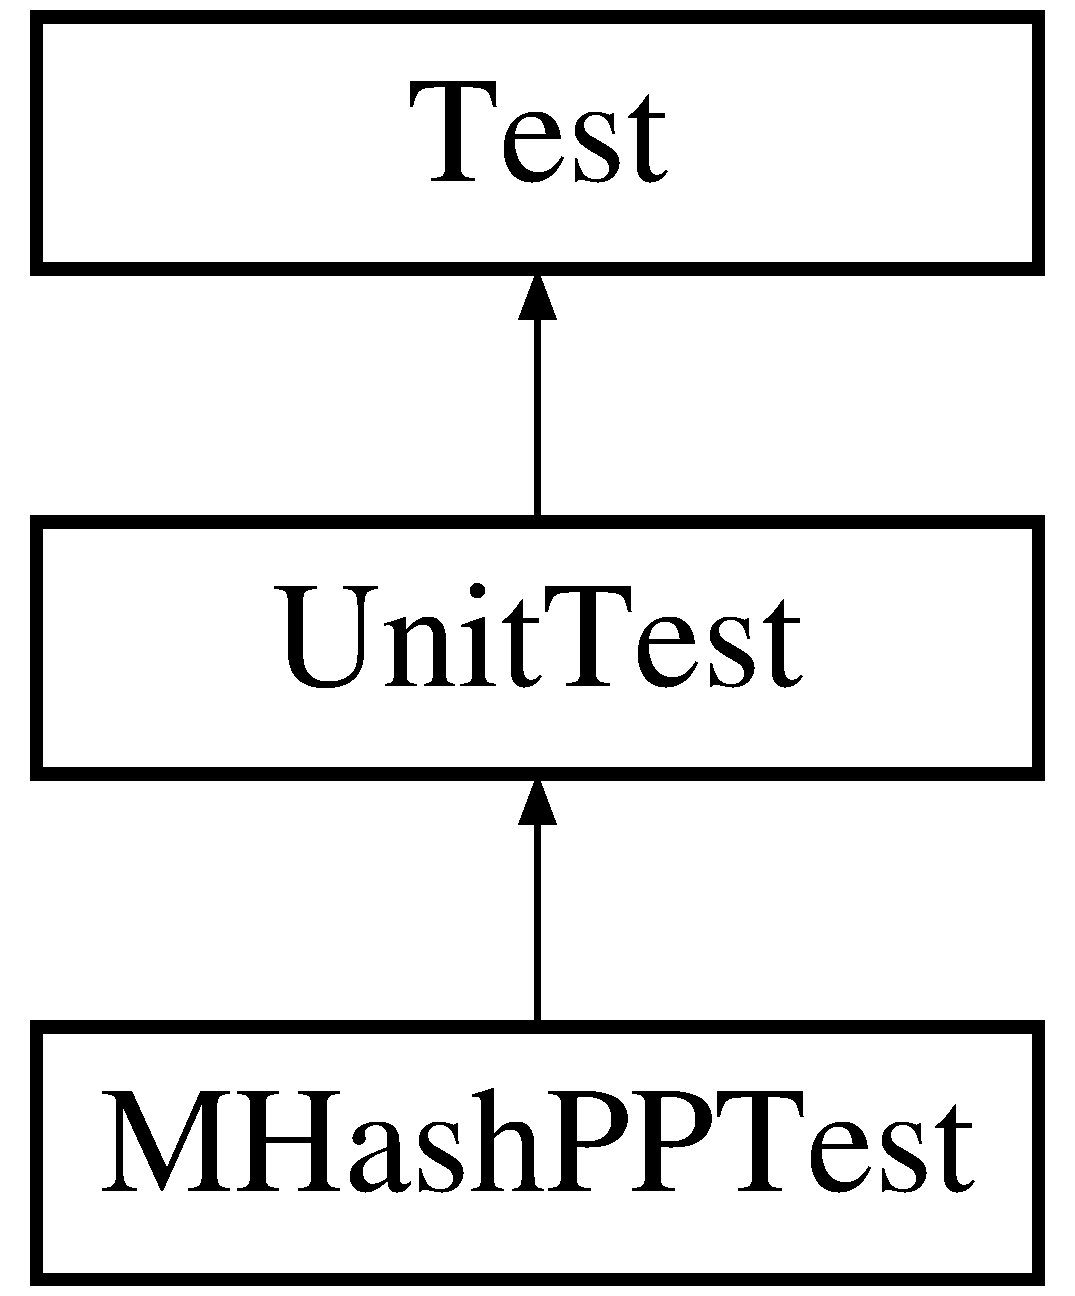
\includegraphics[height=3.000000cm]{classMHashPPTest}
\end{center}
\end{figure}
\subsection*{Public Member Functions}
\begin{DoxyCompactItemize}
\item 
\textbf{ M\+Hash\+P\+P\+Test} (\textbf{ Test\+Suite} $\ast$s)
\item 
void \textbf{ test\+M\+D5} (void)
\item 
void \textbf{ test\+C\+R\+C32} (void)
\end{DoxyCompactItemize}
\subsection*{Private Member Functions}
\begin{DoxyCompactItemize}
\item 
bool \textbf{ generic\+Test\+M\+Hash\+PP} (hashid a, \textbf{ Bit\+String} data, \textbf{ B\+Y\+TE} $\ast$shouldbe)
\end{DoxyCompactItemize}
\subsection*{Additional Inherited Members}


\subsection{Constructor \& Destructor Documentation}
\mbox{\label{classMHashPPTest_aa7b0e8282de3bec1c6a19908693d5df1}} 
\index{M\+Hash\+P\+P\+Test@{M\+Hash\+P\+P\+Test}!M\+Hash\+P\+P\+Test@{M\+Hash\+P\+P\+Test}}
\index{M\+Hash\+P\+P\+Test@{M\+Hash\+P\+P\+Test}!M\+Hash\+P\+P\+Test@{M\+Hash\+P\+P\+Test}}
\subsubsection{M\+Hash\+P\+P\+Test()}
{\footnotesize\ttfamily M\+Hash\+P\+P\+Test\+::\+M\+Hash\+P\+P\+Test (\begin{DoxyParamCaption}\item[{\textbf{ Test\+Suite} $\ast$}]{s }\end{DoxyParamCaption})}



\subsection{Member Function Documentation}
\mbox{\label{classMHashPPTest_abdcae7036faf958977b8cb9193a15303}} 
\index{M\+Hash\+P\+P\+Test@{M\+Hash\+P\+P\+Test}!generic\+Test\+M\+Hash\+PP@{generic\+Test\+M\+Hash\+PP}}
\index{generic\+Test\+M\+Hash\+PP@{generic\+Test\+M\+Hash\+PP}!M\+Hash\+P\+P\+Test@{M\+Hash\+P\+P\+Test}}
\subsubsection{generic\+Test\+M\+Hash\+P\+P()}
{\footnotesize\ttfamily bool M\+Hash\+P\+P\+Test\+::generic\+Test\+M\+Hash\+PP (\begin{DoxyParamCaption}\item[{hashid}]{a,  }\item[{\textbf{ Bit\+String}}]{data,  }\item[{\textbf{ B\+Y\+TE} $\ast$}]{shouldbe }\end{DoxyParamCaption})\hspace{0.3cm}{\ttfamily [private]}}

compute a hash using \doxyref{M\+Hash\+PP}{p.}{classMHashPP} and compare it to a reference value 
\begin{DoxyParams}{Parameters}
{\em a} & the hash algorithm that should be used by \doxyref{M\+Hash\+PP}{p.}{classMHashPP} \\
\hline
{\em data} & the input of the hash algorithm \\
\hline
{\em shouldbe} & the reference value of the result of the hash algorithm \\
\hline
\end{DoxyParams}
\begin{DoxyReturn}{Returns}
true iff shouldbe is the result of the hash algorithm a applied to data by \doxyref{M\+Hash\+PP}{p.}{classMHashPP} 
\end{DoxyReturn}
\mbox{\label{classMHashPPTest_a6b5b8beed154c913654549f521a2d7f2}} 
\index{M\+Hash\+P\+P\+Test@{M\+Hash\+P\+P\+Test}!test\+C\+R\+C32@{test\+C\+R\+C32}}
\index{test\+C\+R\+C32@{test\+C\+R\+C32}!M\+Hash\+P\+P\+Test@{M\+Hash\+P\+P\+Test}}
\subsubsection{test\+C\+R\+C32()}
{\footnotesize\ttfamily void M\+Hash\+P\+P\+Test\+::test\+C\+R\+C32 (\begin{DoxyParamCaption}\item[{void}]{ }\end{DoxyParamCaption})}

\mbox{\label{classMHashPPTest_acff33e798e12a739c9709ff176243d9c}} 
\index{M\+Hash\+P\+P\+Test@{M\+Hash\+P\+P\+Test}!test\+M\+D5@{test\+M\+D5}}
\index{test\+M\+D5@{test\+M\+D5}!M\+Hash\+P\+P\+Test@{M\+Hash\+P\+P\+Test}}
\subsubsection{test\+M\+D5()}
{\footnotesize\ttfamily void M\+Hash\+P\+P\+Test\+::test\+M\+D5 (\begin{DoxyParamCaption}\item[{void}]{ }\end{DoxyParamCaption})}

test output of \doxyref{M\+Hash\+PP}{p.}{classMHashPP} class with M\+D5 algorithm against the test vectors given in R\+FC 1321 

The documentation for this class was generated from the following files\+:\begin{DoxyCompactItemize}
\item 
\textbf{ M\+Hash\+P\+P\+Test.\+h}\item 
\textbf{ M\+Hash\+P\+P\+Test.\+cc}\end{DoxyCompactItemize}

\section{Not\+Implemented\+Error Class Reference}
\label{classNotImplementedError}\index{Not\+Implemented\+Error@{Not\+Implemented\+Error}}


{\ttfamily \#include $<$error.\+h$>$}

Inheritance diagram for Not\+Implemented\+Error\+:\begin{figure}[H]
\begin{center}
\leavevmode
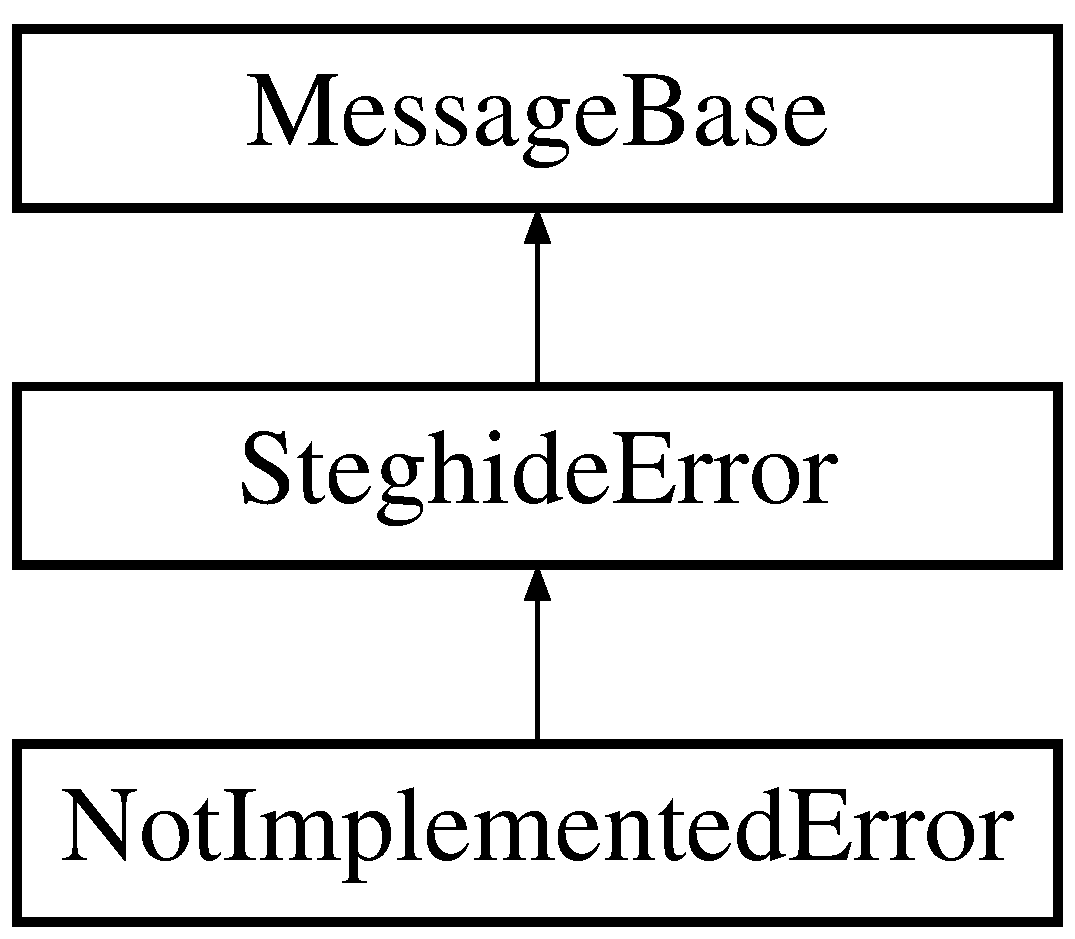
\includegraphics[height=3.000000cm]{classNotImplementedError}
\end{center}
\end{figure}
\subsection*{Public Member Functions}
\begin{DoxyCompactItemize}
\item 
\textbf{ Not\+Implemented\+Error} (const char $\ast$msgfmt,...)
\item 
void \textbf{ print\+Message} (void) const
\end{DoxyCompactItemize}
\subsection*{Additional Inherited Members}


\subsection{Constructor \& Destructor Documentation}
\mbox{\label{classNotImplementedError_a480b35618a1a76c06a53ff70046c0b4b}} 
\index{Not\+Implemented\+Error@{Not\+Implemented\+Error}!Not\+Implemented\+Error@{Not\+Implemented\+Error}}
\index{Not\+Implemented\+Error@{Not\+Implemented\+Error}!Not\+Implemented\+Error@{Not\+Implemented\+Error}}
\subsubsection{Not\+Implemented\+Error()}
{\footnotesize\ttfamily Not\+Implemented\+Error\+::\+Not\+Implemented\+Error (\begin{DoxyParamCaption}\item[{const char $\ast$}]{msgfmt,  }\item[{}]{... }\end{DoxyParamCaption})}



\subsection{Member Function Documentation}
\mbox{\label{classNotImplementedError_abbe96cc33b89076043f8f71fde80a0cd}} 
\index{Not\+Implemented\+Error@{Not\+Implemented\+Error}!print\+Message@{print\+Message}}
\index{print\+Message@{print\+Message}!Not\+Implemented\+Error@{Not\+Implemented\+Error}}
\subsubsection{print\+Message()}
{\footnotesize\ttfamily void Not\+Implemented\+Error\+::print\+Message (\begin{DoxyParamCaption}\item[{void}]{ }\end{DoxyParamCaption}) const\hspace{0.3cm}{\ttfamily [virtual]}}



Reimplemented from \textbf{ Steghide\+Error} \doxyref{}{p.}{classSteghideError_a22d688da944706920f51159ebd0076d9}.



The documentation for this class was generated from the following files\+:\begin{DoxyCompactItemize}
\item 
\textbf{ error.\+h}\item 
\textbf{ error.\+cc}\end{DoxyCompactItemize}

\section{Progress\+Output Class Reference}
\label{classProgressOutput}\index{Progress\+Output@{Progress\+Output}}


prints the progress to stdout  




{\ttfamily \#include $<$Progress\+Output.\+h$>$}

\subsection*{Public Member Functions}
\begin{DoxyCompactItemize}
\item 
\textbf{ Progress\+Output} (void)
\item 
\textbf{ Progress\+Output} (const std\+::string \&m)
\item 
void \textbf{ set\+Message} (const std\+::string \&m)
\item 
void \textbf{ set\+Message} (const char $\ast$msgfmt,...)
\item 
void \textbf{ update} (float rate)
\item 
void \textbf{ done} (void) const
\item 
void \textbf{ done} (float rate, float avgweight=\textbf{ No\+Avg\+Weight}) const
\end{DoxyCompactItemize}
\subsection*{Static Public Attributes}
\begin{DoxyCompactItemize}
\item 
static const float \textbf{ No\+Avg\+Weight} = -\/1.\+0
\end{DoxyCompactItemize}
\subsection*{Protected Member Functions}
\begin{DoxyCompactItemize}
\item 
std\+::string \textbf{ vcompose} (const char $\ast$msgfmt, va\+\_\+list ap) const
\end{DoxyCompactItemize}
\subsection*{Private Attributes}
\begin{DoxyCompactItemize}
\item 
std\+::string \textbf{ Message}
\item 
time\+\_\+t \textbf{ Last\+Update}
\end{DoxyCompactItemize}


\subsection{Constructor \& Destructor Documentation}
\mbox{\label{classProgressOutput_a3bcb9ceb59b9692bdc1e4ad21a258776}} 
\index{Progress\+Output@{Progress\+Output}!Progress\+Output@{Progress\+Output}}
\index{Progress\+Output@{Progress\+Output}!Progress\+Output@{Progress\+Output}}
\subsubsection{Progress\+Output()\hspace{0.1cm}{\footnotesize\ttfamily [1/2]}}
{\footnotesize\ttfamily Progress\+Output\+::\+Progress\+Output (\begin{DoxyParamCaption}\item[{void}]{ }\end{DoxyParamCaption})}

create an empty \doxyref{Progress\+Output}{p.}{classProgressOutput} object \mbox{\label{classProgressOutput_a152c668bd24d44d4ba3fabab1228cda2}} 
\index{Progress\+Output@{Progress\+Output}!Progress\+Output@{Progress\+Output}}
\index{Progress\+Output@{Progress\+Output}!Progress\+Output@{Progress\+Output}}
\subsubsection{Progress\+Output()\hspace{0.1cm}{\footnotesize\ttfamily [2/2]}}
{\footnotesize\ttfamily Progress\+Output\+::\+Progress\+Output (\begin{DoxyParamCaption}\item[{const std\+::string \&}]{m }\end{DoxyParamCaption})}

create a \doxyref{Progress\+Output}{p.}{classProgressOutput} object 
\begin{DoxyParams}{Parameters}
{\em m} & the message to be displayed \\
\hline
\end{DoxyParams}


\subsection{Member Function Documentation}
\mbox{\label{classProgressOutput_ab9500306bfb6f2585ea5b28d9a217d97}} 
\index{Progress\+Output@{Progress\+Output}!done@{done}}
\index{done@{done}!Progress\+Output@{Progress\+Output}}
\subsubsection{done()\hspace{0.1cm}{\footnotesize\ttfamily [1/2]}}
{\footnotesize\ttfamily void Progress\+Output\+::done (\begin{DoxyParamCaption}\item[{void}]{ }\end{DoxyParamCaption}) const}

update the output appending \char`\"{}done\char`\"{} and a newline (no rate nor average weight) \mbox{\label{classProgressOutput_ac46bf29a71369f33bd936d4cc6fbd82c}} 
\index{Progress\+Output@{Progress\+Output}!done@{done}}
\index{done@{done}!Progress\+Output@{Progress\+Output}}
\subsubsection{done()\hspace{0.1cm}{\footnotesize\ttfamily [2/2]}}
{\footnotesize\ttfamily void Progress\+Output\+::done (\begin{DoxyParamCaption}\item[{float}]{rate,  }\item[{float}]{avgweight = {\ttfamily \textbf{ No\+Avg\+Weight}} }\end{DoxyParamCaption}) const}

update the output appending rate, [average edge weight], \char`\"{}done\char`\"{} and a newline 
\begin{DoxyParams}{Parameters}
{\em rate} & the rate of matched vertices \\
\hline
{\em avgweight} & the average edge weight (is not printed if not given) \\
\hline
\end{DoxyParams}
\mbox{\label{classProgressOutput_a0855ccf4fb1ebfd3af608070eb1d4a71}} 
\index{Progress\+Output@{Progress\+Output}!set\+Message@{set\+Message}}
\index{set\+Message@{set\+Message}!Progress\+Output@{Progress\+Output}}
\subsubsection{set\+Message()\hspace{0.1cm}{\footnotesize\ttfamily [1/2]}}
{\footnotesize\ttfamily void Progress\+Output\+::set\+Message (\begin{DoxyParamCaption}\item[{const std\+::string \&}]{m }\end{DoxyParamCaption})\hspace{0.3cm}{\ttfamily [inline]}}

\mbox{\label{classProgressOutput_af1baf2a638d4003ff77eebc075ef30e4}} 
\index{Progress\+Output@{Progress\+Output}!set\+Message@{set\+Message}}
\index{set\+Message@{set\+Message}!Progress\+Output@{Progress\+Output}}
\subsubsection{set\+Message()\hspace{0.1cm}{\footnotesize\ttfamily [2/2]}}
{\footnotesize\ttfamily void Progress\+Output\+::set\+Message (\begin{DoxyParamCaption}\item[{const char $\ast$}]{msgfmt,  }\item[{}]{... }\end{DoxyParamCaption})}

\mbox{\label{classProgressOutput_afa50b8bcf85f139caa01495479b3849b}} 
\index{Progress\+Output@{Progress\+Output}!update@{update}}
\index{update@{update}!Progress\+Output@{Progress\+Output}}
\subsubsection{update()}
{\footnotesize\ttfamily void Progress\+Output\+::update (\begin{DoxyParamCaption}\item[{float}]{rate }\end{DoxyParamCaption})}

update the output (taking update frequency into account) with rate as percentage \mbox{\label{classProgressOutput_a46454cbf5d2a9e7cf8b6af61874b8f2e}} 
\index{Progress\+Output@{Progress\+Output}!vcompose@{vcompose}}
\index{vcompose@{vcompose}!Progress\+Output@{Progress\+Output}}
\subsubsection{vcompose()}
{\footnotesize\ttfamily std\+::string Progress\+Output\+::vcompose (\begin{DoxyParamCaption}\item[{const char $\ast$}]{msgfmt,  }\item[{va\+\_\+list}]{ap }\end{DoxyParamCaption}) const\hspace{0.3cm}{\ttfamily [protected]}}



\subsection{Member Data Documentation}
\mbox{\label{classProgressOutput_a1786e9955e0ef66f3806c4d7a7818f6d}} 
\index{Progress\+Output@{Progress\+Output}!Last\+Update@{Last\+Update}}
\index{Last\+Update@{Last\+Update}!Progress\+Output@{Progress\+Output}}
\subsubsection{Last\+Update}
{\footnotesize\ttfamily time\+\_\+t Progress\+Output\+::\+Last\+Update\hspace{0.3cm}{\ttfamily [private]}}

\mbox{\label{classProgressOutput_a9cac63691979785d388daa94051468be}} 
\index{Progress\+Output@{Progress\+Output}!Message@{Message}}
\index{Message@{Message}!Progress\+Output@{Progress\+Output}}
\subsubsection{Message}
{\footnotesize\ttfamily std\+::string Progress\+Output\+::\+Message\hspace{0.3cm}{\ttfamily [private]}}

\mbox{\label{classProgressOutput_ac72839c165b28e001209dfce3c8ba9d1}} 
\index{Progress\+Output@{Progress\+Output}!No\+Avg\+Weight@{No\+Avg\+Weight}}
\index{No\+Avg\+Weight@{No\+Avg\+Weight}!Progress\+Output@{Progress\+Output}}
\subsubsection{No\+Avg\+Weight}
{\footnotesize\ttfamily const float Progress\+Output\+::\+No\+Avg\+Weight = -\/1.\+0\hspace{0.3cm}{\ttfamily [static]}}



The documentation for this class was generated from the following files\+:\begin{DoxyCompactItemize}
\item 
\textbf{ Progress\+Output.\+h}\item 
\textbf{ Progress\+Output.\+cc}\end{DoxyCompactItemize}

\section{Cvr\+Stg\+File\+:\+:Property Class Reference}
\label{classCvrStgFile_1_1Property}\index{Cvr\+Stg\+File\+::\+Property@{Cvr\+Stg\+File\+::\+Property}}


{\ttfamily \#include $<$Cvr\+Stg\+File.\+h$>$}

Inheritance diagram for Cvr\+Stg\+File\+:\+:Property\+:\begin{figure}[H]
\begin{center}
\leavevmode
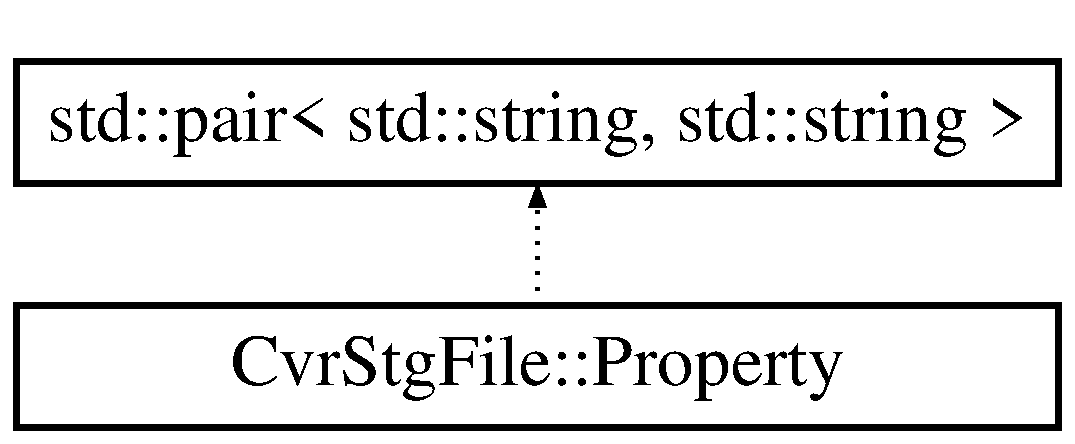
\includegraphics[height=2.000000cm]{classCvrStgFile_1_1Property}
\end{center}
\end{figure}
\subsection*{Public Member Functions}
\begin{DoxyCompactItemize}
\item 
\textbf{ Property} (std\+::string key, std\+::string value)
\item 
std\+::string \textbf{ get\+Key} (void) const
\item 
std\+::string \textbf{ get\+Value} (void) const
\end{DoxyCompactItemize}


\subsection{Constructor \& Destructor Documentation}
\mbox{\label{classCvrStgFile_1_1Property_a7c1f7709cb31dcef8d71a10dc194e861}} 
\index{Cvr\+Stg\+File\+::\+Property@{Cvr\+Stg\+File\+::\+Property}!Property@{Property}}
\index{Property@{Property}!Cvr\+Stg\+File\+::\+Property@{Cvr\+Stg\+File\+::\+Property}}
\subsubsection{Property()}
{\footnotesize\ttfamily Cvr\+Stg\+File\+::\+Property\+::\+Property (\begin{DoxyParamCaption}\item[{std\+::string}]{key,  }\item[{std\+::string}]{value }\end{DoxyParamCaption})\hspace{0.3cm}{\ttfamily [inline]}}



\subsection{Member Function Documentation}
\mbox{\label{classCvrStgFile_1_1Property_af68b007967b59ec9b6d0de644172be53}} 
\index{Cvr\+Stg\+File\+::\+Property@{Cvr\+Stg\+File\+::\+Property}!get\+Key@{get\+Key}}
\index{get\+Key@{get\+Key}!Cvr\+Stg\+File\+::\+Property@{Cvr\+Stg\+File\+::\+Property}}
\subsubsection{get\+Key()}
{\footnotesize\ttfamily std\+::string Cvr\+Stg\+File\+::\+Property\+::get\+Key (\begin{DoxyParamCaption}\item[{void}]{ }\end{DoxyParamCaption}) const\hspace{0.3cm}{\ttfamily [inline]}}

\mbox{\label{classCvrStgFile_1_1Property_ae3bce21141df6d353e83b1b290e85bdf}} 
\index{Cvr\+Stg\+File\+::\+Property@{Cvr\+Stg\+File\+::\+Property}!get\+Value@{get\+Value}}
\index{get\+Value@{get\+Value}!Cvr\+Stg\+File\+::\+Property@{Cvr\+Stg\+File\+::\+Property}}
\subsubsection{get\+Value()}
{\footnotesize\ttfamily std\+::string Cvr\+Stg\+File\+::\+Property\+::get\+Value (\begin{DoxyParamCaption}\item[{void}]{ }\end{DoxyParamCaption}) const\hspace{0.3cm}{\ttfamily [inline]}}



The documentation for this class was generated from the following file\+:\begin{DoxyCompactItemize}
\item 
\textbf{ Cvr\+Stg\+File.\+h}\end{DoxyCompactItemize}

\section{Pseudo\+Random\+Source Class Reference}
\label{classPseudoRandomSource}\index{Pseudo\+Random\+Source@{Pseudo\+Random\+Source}}


this class serves as a source of reproducible (pseudo-\/)random numbers  




{\ttfamily \#include $<$Pseudo\+Random\+Source.\+h$>$}

\subsection*{Public Member Functions}
\begin{DoxyCompactItemize}
\item 
\textbf{ Pseudo\+Random\+Source} (\textbf{ U\+W\+O\+R\+D32} s)
\item 
\textbf{ U\+W\+O\+R\+D32} \textbf{ get\+Value} (\textbf{ U\+W\+O\+R\+D32} n)
\end{DoxyCompactItemize}
\subsection*{Private Attributes}
\begin{DoxyCompactItemize}
\item 
\textbf{ U\+W\+O\+R\+D32} \textbf{ Value}
\end{DoxyCompactItemize}
\subsection*{Static Private Attributes}
\begin{DoxyCompactItemize}
\item 
static const \textbf{ U\+W\+O\+R\+D32} \textbf{ A} = 1367208549
\item 
static const \textbf{ U\+W\+O\+R\+D32} \textbf{ C} = 1
\end{DoxyCompactItemize}


\subsection{Detailed Description}
To generate the random numbers, the linear congruetial method is used. 2$^\wedge$32 is used as modulus. The overflow in the implementation is intended (and controlled, as U\+W\+O\+R\+D32 is used as datatype which always is 32 bits wide). 

\subsection{Constructor \& Destructor Documentation}
\mbox{\label{classPseudoRandomSource_a99178fce83f11ef778d93c125d8b0638}} 
\index{Pseudo\+Random\+Source@{Pseudo\+Random\+Source}!Pseudo\+Random\+Source@{Pseudo\+Random\+Source}}
\index{Pseudo\+Random\+Source@{Pseudo\+Random\+Source}!Pseudo\+Random\+Source@{Pseudo\+Random\+Source}}
\subsubsection{Pseudo\+Random\+Source()}
{\footnotesize\ttfamily Pseudo\+Random\+Source\+::\+Pseudo\+Random\+Source (\begin{DoxyParamCaption}\item[{\textbf{ U\+W\+O\+R\+D32}}]{s }\end{DoxyParamCaption})\hspace{0.3cm}{\ttfamily [inline]}}

construct a \doxyref{Pseudo\+Random\+Source}{p.}{classPseudoRandomSource} object 
\begin{DoxyParams}{Parameters}
{\em s} & the seed \\
\hline
\end{DoxyParams}


\subsection{Member Function Documentation}
\mbox{\label{classPseudoRandomSource_a8ef2aa9bb5419cbaf1d7a28f958115f9}} 
\index{Pseudo\+Random\+Source@{Pseudo\+Random\+Source}!get\+Value@{get\+Value}}
\index{get\+Value@{get\+Value}!Pseudo\+Random\+Source@{Pseudo\+Random\+Source}}
\subsubsection{get\+Value()}
{\footnotesize\ttfamily \textbf{ U\+W\+O\+R\+D32} Pseudo\+Random\+Source\+::get\+Value (\begin{DoxyParamCaption}\item[{\textbf{ U\+W\+O\+R\+D32}}]{n }\end{DoxyParamCaption})}

get a pseudo-\/random value from \{0,...,n-\/1\} 
\begin{DoxyParams}{Parameters}
{\em n} & the range of the random value to be returned \\
\hline
\end{DoxyParams}
\begin{DoxyReturn}{Returns}
a number $>$= 0 and $<$= n -\/ 1
\end{DoxyReturn}
After calling get\+Value, the next get\+Value call will use the next state of the random number generator (analogous to the C rand() function) 

\subsection{Member Data Documentation}
\mbox{\label{classPseudoRandomSource_a5b780fa93c41e7057e00e44faaaa2dca}} 
\index{Pseudo\+Random\+Source@{Pseudo\+Random\+Source}!A@{A}}
\index{A@{A}!Pseudo\+Random\+Source@{Pseudo\+Random\+Source}}
\subsubsection{A}
{\footnotesize\ttfamily const \textbf{ U\+W\+O\+R\+D32} Pseudo\+Random\+Source\+::A = 1367208549\hspace{0.3cm}{\ttfamily [static]}, {\ttfamily [private]}}

\mbox{\label{classPseudoRandomSource_a4a35b7e561bfcf7c8031ce0e985a992e}} 
\index{Pseudo\+Random\+Source@{Pseudo\+Random\+Source}!C@{C}}
\index{C@{C}!Pseudo\+Random\+Source@{Pseudo\+Random\+Source}}
\subsubsection{C}
{\footnotesize\ttfamily const \textbf{ U\+W\+O\+R\+D32} Pseudo\+Random\+Source\+::C = 1\hspace{0.3cm}{\ttfamily [static]}, {\ttfamily [private]}}

\mbox{\label{classPseudoRandomSource_a7b82ea9bcac4633974b9d10f260d3f4e}} 
\index{Pseudo\+Random\+Source@{Pseudo\+Random\+Source}!Value@{Value}}
\index{Value@{Value}!Pseudo\+Random\+Source@{Pseudo\+Random\+Source}}
\subsubsection{Value}
{\footnotesize\ttfamily \textbf{ U\+W\+O\+R\+D32} Pseudo\+Random\+Source\+::\+Value\hspace{0.3cm}{\ttfamily [private]}}



The documentation for this class was generated from the following files\+:\begin{DoxyCompactItemize}
\item 
\textbf{ Pseudo\+Random\+Source.\+h}\item 
\textbf{ Pseudo\+Random\+Source.\+cc}\end{DoxyCompactItemize}

\section{Question Class Reference}
\label{classQuestion}\index{Question@{Question}}


{\ttfamily \#include $<$msg.\+h$>$}

Inheritance diagram for Question\+:\begin{figure}[H]
\begin{center}
\leavevmode
\includegraphics[height=2.000000cm]{classQuestion}
\end{center}
\end{figure}
\subsection*{Public Member Functions}
\begin{DoxyCompactItemize}
\item 
\textbf{ Question} (void)
\item 
\textbf{ Question} (std\+::string msg)
\item 
\textbf{ Question} (const char $\ast$msgfmt,...)
\item 
void \textbf{ print\+Message} (void) const
\item 
bool \textbf{ get\+Answer} (void)
\end{DoxyCompactItemize}
\subsection*{Private Attributes}
\begin{DoxyCompactItemize}
\item 
std\+::string \textbf{ yeschar}
\item 
std\+::string \textbf{ nochar}
\end{DoxyCompactItemize}
\subsection*{Additional Inherited Members}


\subsection{Constructor \& Destructor Documentation}
\mbox{\label{classQuestion_a135d047e1f35ce94e7668505b727c20c}} 
\index{Question@{Question}!Question@{Question}}
\index{Question@{Question}!Question@{Question}}
\subsubsection{Question()\hspace{0.1cm}{\footnotesize\ttfamily [1/3]}}
{\footnotesize\ttfamily Question\+::\+Question (\begin{DoxyParamCaption}\item[{void}]{ }\end{DoxyParamCaption})}

\mbox{\label{classQuestion_a8f1451cd8bc72891f33c80a52ece51b4}} 
\index{Question@{Question}!Question@{Question}}
\index{Question@{Question}!Question@{Question}}
\subsubsection{Question()\hspace{0.1cm}{\footnotesize\ttfamily [2/3]}}
{\footnotesize\ttfamily Question\+::\+Question (\begin{DoxyParamCaption}\item[{std\+::string}]{msg }\end{DoxyParamCaption})}

\mbox{\label{classQuestion_ab11e3e5ec83c510a217964d3ab2edc40}} 
\index{Question@{Question}!Question@{Question}}
\index{Question@{Question}!Question@{Question}}
\subsubsection{Question()\hspace{0.1cm}{\footnotesize\ttfamily [3/3]}}
{\footnotesize\ttfamily Question\+::\+Question (\begin{DoxyParamCaption}\item[{const char $\ast$}]{msgfmt,  }\item[{}]{... }\end{DoxyParamCaption})}



\subsection{Member Function Documentation}
\mbox{\label{classQuestion_ada436c3b56eb8b46bc9aad8af47279e4}} 
\index{Question@{Question}!get\+Answer@{get\+Answer}}
\index{get\+Answer@{get\+Answer}!Question@{Question}}
\subsubsection{get\+Answer()}
{\footnotesize\ttfamily bool Question\+::get\+Answer (\begin{DoxyParamCaption}\item[{void}]{ }\end{DoxyParamCaption})}

wait for the user to answer the question (should be printed before) \begin{DoxyReturn}{Returns}
true iff the user answers with yes, i.\+e. presses the yeschar-\/key 
\end{DoxyReturn}
\mbox{\label{classQuestion_a5b0fe8561addc6710984b02b34cfe68c}} 
\index{Question@{Question}!print\+Message@{print\+Message}}
\index{print\+Message@{print\+Message}!Question@{Question}}
\subsubsection{print\+Message()}
{\footnotesize\ttfamily void Question\+::print\+Message (\begin{DoxyParamCaption}\item[{void}]{ }\end{DoxyParamCaption}) const\hspace{0.3cm}{\ttfamily [virtual]}}



Implements \textbf{ Message\+Base} \doxyref{}{p.}{classMessageBase_a207178190da2bec546a972495cdf9bc6}.



\subsection{Member Data Documentation}
\mbox{\label{classQuestion_ad53b548a6db59f4a51c21dcab4072796}} 
\index{Question@{Question}!nochar@{nochar}}
\index{nochar@{nochar}!Question@{Question}}
\subsubsection{nochar}
{\footnotesize\ttfamily std\+::string Question\+::nochar\hspace{0.3cm}{\ttfamily [private]}}

\mbox{\label{classQuestion_aa9644e0c50afcbedd7eaaba5966ad3e6}} 
\index{Question@{Question}!yeschar@{yeschar}}
\index{yeschar@{yeschar}!Question@{Question}}
\subsubsection{yeschar}
{\footnotesize\ttfamily std\+::string Question\+::yeschar\hspace{0.3cm}{\ttfamily [private]}}



The documentation for this class was generated from the following files\+:\begin{DoxyCompactItemize}
\item 
\textbf{ msg.\+h}\item 
\textbf{ msg.\+cc}\end{DoxyCompactItemize}

\section{Random\+Source Class Reference}
\label{classRandomSource}\index{Random\+Source@{Random\+Source}}


objects of this class are used as a source of random (non reproduceable) data  




{\ttfamily \#include $<$Random\+Source.\+h$>$}

\subsection*{Public Member Functions}
\begin{DoxyCompactItemize}
\item 
\textbf{ Random\+Source} (void)
\item 
\textbf{ $\sim$\+Random\+Source} (void)
\item 
\textbf{ B\+Y\+TE} \textbf{ get\+Byte} (void)
\item 
std\+::vector$<$ \textbf{ B\+Y\+TE} $>$ \textbf{ get\+Bytes} (unsigned int n)
\item 
\textbf{ Bit\+String} \textbf{ get\+Bits} (unsigned int n)
\item 
bool \textbf{ get\+Bool} (void)
\item 
unsigned long \textbf{ get\+Value} (unsigned long n)
\end{DoxyCompactItemize}
\subsection*{Private Attributes}
\begin{DoxyCompactItemize}
\item 
unsigned int \textbf{ Random\+Byte\+Pos}
\item 
\textbf{ B\+Y\+TE} \textbf{ Random\+Byte}
\item 
F\+I\+LE $\ast$ \textbf{ Random\+Input}
\end{DoxyCompactItemize}


\subsection{Constructor \& Destructor Documentation}
\mbox{\label{classRandomSource_aa6834a1aa7e03c593a6294188016d9b8}} 
\index{Random\+Source@{Random\+Source}!Random\+Source@{Random\+Source}}
\index{Random\+Source@{Random\+Source}!Random\+Source@{Random\+Source}}
\subsubsection{Random\+Source()}
{\footnotesize\ttfamily Random\+Source\+::\+Random\+Source (\begin{DoxyParamCaption}\item[{void}]{ }\end{DoxyParamCaption})}

\mbox{\label{classRandomSource_a36d73775c1660b03707061a03374f8ee}} 
\index{Random\+Source@{Random\+Source}!````~Random\+Source@{$\sim$\+Random\+Source}}
\index{````~Random\+Source@{$\sim$\+Random\+Source}!Random\+Source@{Random\+Source}}
\subsubsection{$\sim$\+Random\+Source()}
{\footnotesize\ttfamily Random\+Source\+::$\sim$\+Random\+Source (\begin{DoxyParamCaption}\item[{void}]{ }\end{DoxyParamCaption})}



\subsection{Member Function Documentation}
\mbox{\label{classRandomSource_aa179ee74465da57ce3f547dd26b894aa}} 
\index{Random\+Source@{Random\+Source}!get\+Bits@{get\+Bits}}
\index{get\+Bits@{get\+Bits}!Random\+Source@{Random\+Source}}
\subsubsection{get\+Bits()}
{\footnotesize\ttfamily \textbf{ Bit\+String} Random\+Source\+::get\+Bits (\begin{DoxyParamCaption}\item[{unsigned int}]{n }\end{DoxyParamCaption})}

get n random bits 
\begin{DoxyParams}{Parameters}
{\em n} & the number of requested random bits \\
\hline
\end{DoxyParams}
\begin{DoxyReturn}{Returns}
a \doxyref{Bit\+String}{p.}{classBitString} containing n random bits 
\end{DoxyReturn}
\mbox{\label{classRandomSource_af88464db6fe07bd9aad36ba0e9c2ccca}} 
\index{Random\+Source@{Random\+Source}!get\+Bool@{get\+Bool}}
\index{get\+Bool@{get\+Bool}!Random\+Source@{Random\+Source}}
\subsubsection{get\+Bool()}
{\footnotesize\ttfamily bool Random\+Source\+::get\+Bool (\begin{DoxyParamCaption}\item[{void}]{ }\end{DoxyParamCaption})}

get a boolean value \begin{DoxyReturn}{Returns}
true of false with equal probability 
\end{DoxyReturn}
\mbox{\label{classRandomSource_aed9b2b297e46a34024fca9f26c205dbc}} 
\index{Random\+Source@{Random\+Source}!get\+Byte@{get\+Byte}}
\index{get\+Byte@{get\+Byte}!Random\+Source@{Random\+Source}}
\subsubsection{get\+Byte()}
{\footnotesize\ttfamily \textbf{ B\+Y\+TE} Random\+Source\+::get\+Byte (\begin{DoxyParamCaption}\item[{void}]{ }\end{DoxyParamCaption})}

get a random byte \begin{DoxyReturn}{Returns}
a random byte 
\end{DoxyReturn}
\mbox{\label{classRandomSource_a5e9f3b244d0e3f8cb1d3c29aa2702a54}} 
\index{Random\+Source@{Random\+Source}!get\+Bytes@{get\+Bytes}}
\index{get\+Bytes@{get\+Bytes}!Random\+Source@{Random\+Source}}
\subsubsection{get\+Bytes()}
{\footnotesize\ttfamily std\+::vector$<$ \textbf{ B\+Y\+TE} $>$ Random\+Source\+::get\+Bytes (\begin{DoxyParamCaption}\item[{unsigned int}]{n }\end{DoxyParamCaption})}

get n random bytes 
\begin{DoxyParams}{Parameters}
{\em n} & the number of requested random bytes \\
\hline
\end{DoxyParams}
\begin{DoxyReturn}{Returns}
n random bytes 
\end{DoxyReturn}
\mbox{\label{classRandomSource_a36229e10b935fc34a0ea9151cdcf253f}} 
\index{Random\+Source@{Random\+Source}!get\+Value@{get\+Value}}
\index{get\+Value@{get\+Value}!Random\+Source@{Random\+Source}}
\subsubsection{get\+Value()}
{\footnotesize\ttfamily unsigned long Random\+Source\+::get\+Value (\begin{DoxyParamCaption}\item[{unsigned long}]{n }\end{DoxyParamCaption})}

get a random value 
\begin{DoxyParams}{Parameters}
{\em n} & the range of the random value to be returned \\
\hline
\end{DoxyParams}
\begin{DoxyReturn}{Returns}
a random number in \{0,...,n-\/1\} 
\end{DoxyReturn}


\subsection{Member Data Documentation}
\mbox{\label{classRandomSource_a8ca93a71e1ba9aaf8cb6fe4f8d65dfde}} 
\index{Random\+Source@{Random\+Source}!Random\+Byte@{Random\+Byte}}
\index{Random\+Byte@{Random\+Byte}!Random\+Source@{Random\+Source}}
\subsubsection{Random\+Byte}
{\footnotesize\ttfamily \textbf{ B\+Y\+TE} Random\+Source\+::\+Random\+Byte\hspace{0.3cm}{\ttfamily [private]}}

\mbox{\label{classRandomSource_a43389d89f5be07bc777ad87c435939be}} 
\index{Random\+Source@{Random\+Source}!Random\+Byte\+Pos@{Random\+Byte\+Pos}}
\index{Random\+Byte\+Pos@{Random\+Byte\+Pos}!Random\+Source@{Random\+Source}}
\subsubsection{Random\+Byte\+Pos}
{\footnotesize\ttfamily unsigned int Random\+Source\+::\+Random\+Byte\+Pos\hspace{0.3cm}{\ttfamily [private]}}

\mbox{\label{classRandomSource_aa9015ccb1b35282da7273963b4a58ccd}} 
\index{Random\+Source@{Random\+Source}!Random\+Input@{Random\+Input}}
\index{Random\+Input@{Random\+Input}!Random\+Source@{Random\+Source}}
\subsubsection{Random\+Input}
{\footnotesize\ttfamily F\+I\+LE$\ast$ Random\+Source\+::\+Random\+Input\hspace{0.3cm}{\ttfamily [private]}}

determines the random input -\/ is either opened file pointer to /dev/urandom or N\+U\+LL (the rand() function is then used as random source) 

The documentation for this class was generated from the following files\+:\begin{DoxyCompactItemize}
\item 
\textbf{ Random\+Source.\+h}\item 
\textbf{ Random\+Source.\+cc}\end{DoxyCompactItemize}

\section{R\+G\+B\+Triple Class Reference}
\label{classRGBTriple}\index{R\+G\+B\+Triple@{R\+G\+B\+Triple}}


{\ttfamily \#include $<$R\+G\+B\+Triple.\+h$>$}

\subsection*{Public Member Functions}
\begin{DoxyCompactItemize}
\item 
\textbf{ R\+G\+B\+Triple} (void)
\item 
\textbf{ R\+G\+B\+Triple} (\textbf{ B\+Y\+TE} r, \textbf{ B\+Y\+TE} g, \textbf{ B\+Y\+TE} b)
\item 
\textbf{ U\+W\+O\+R\+D32} \textbf{ calc\+Distance} (const \textbf{ R\+G\+B\+Triple} \&t) const
\item 
bool \textbf{ operator==} (const \textbf{ R\+G\+B\+Triple} \&t) const
\item 
bool \textbf{ operator!=} (const \textbf{ R\+G\+B\+Triple} \&t) const
\end{DoxyCompactItemize}
\subsection*{Public Attributes}
\begin{DoxyCompactItemize}
\item 
\textbf{ B\+Y\+TE} \textbf{ Red}
\item 
\textbf{ B\+Y\+TE} \textbf{ Green}
\item 
\textbf{ B\+Y\+TE} \textbf{ Blue}
\end{DoxyCompactItemize}


\subsection{Constructor \& Destructor Documentation}
\mbox{\label{classRGBTriple_aab572f447086df43db5d08b4c3b75199}} 
\index{R\+G\+B\+Triple@{R\+G\+B\+Triple}!R\+G\+B\+Triple@{R\+G\+B\+Triple}}
\index{R\+G\+B\+Triple@{R\+G\+B\+Triple}!R\+G\+B\+Triple@{R\+G\+B\+Triple}}
\subsubsection{R\+G\+B\+Triple()\hspace{0.1cm}{\footnotesize\ttfamily [1/2]}}
{\footnotesize\ttfamily R\+G\+B\+Triple\+::\+R\+G\+B\+Triple (\begin{DoxyParamCaption}\item[{void}]{ }\end{DoxyParamCaption})\hspace{0.3cm}{\ttfamily [inline]}}

\mbox{\label{classRGBTriple_a47459117a129f99faf57260fb39d0a85}} 
\index{R\+G\+B\+Triple@{R\+G\+B\+Triple}!R\+G\+B\+Triple@{R\+G\+B\+Triple}}
\index{R\+G\+B\+Triple@{R\+G\+B\+Triple}!R\+G\+B\+Triple@{R\+G\+B\+Triple}}
\subsubsection{R\+G\+B\+Triple()\hspace{0.1cm}{\footnotesize\ttfamily [2/2]}}
{\footnotesize\ttfamily R\+G\+B\+Triple\+::\+R\+G\+B\+Triple (\begin{DoxyParamCaption}\item[{\textbf{ B\+Y\+TE}}]{r,  }\item[{\textbf{ B\+Y\+TE}}]{g,  }\item[{\textbf{ B\+Y\+TE}}]{b }\end{DoxyParamCaption})\hspace{0.3cm}{\ttfamily [inline]}}



\subsection{Member Function Documentation}
\mbox{\label{classRGBTriple_aa8a50821a88d11a5e8f2a7fc7ed31958}} 
\index{R\+G\+B\+Triple@{R\+G\+B\+Triple}!calc\+Distance@{calc\+Distance}}
\index{calc\+Distance@{calc\+Distance}!R\+G\+B\+Triple@{R\+G\+B\+Triple}}
\subsubsection{calc\+Distance()}
{\footnotesize\ttfamily \textbf{ U\+W\+O\+R\+D32} R\+G\+B\+Triple\+::calc\+Distance (\begin{DoxyParamCaption}\item[{const \textbf{ R\+G\+B\+Triple} \&}]{t }\end{DoxyParamCaption}) const}

get the squared distance in the R\+GB cube between this triple and the triple t 
\begin{DoxyParams}{Parameters}
{\em t} & another R\+GB triple \\
\hline
\end{DoxyParams}
\begin{DoxyReturn}{Returns}
the square of the euclidean distance between this and t 
\end{DoxyReturn}
\mbox{\label{classRGBTriple_a00ec6e847926e1d0484f76dc899b399b}} 
\index{R\+G\+B\+Triple@{R\+G\+B\+Triple}!operator"!=@{operator"!=}}
\index{operator"!=@{operator"!=}!R\+G\+B\+Triple@{R\+G\+B\+Triple}}
\subsubsection{operator"!=()}
{\footnotesize\ttfamily bool R\+G\+B\+Triple\+::operator!= (\begin{DoxyParamCaption}\item[{const \textbf{ R\+G\+B\+Triple} \&}]{t }\end{DoxyParamCaption}) const}

return true iff this triple and t are not equal (i.\+e. have different rgb values) \mbox{\label{classRGBTriple_a1c795b3d57cc4e1efa775130fa15f277}} 
\index{R\+G\+B\+Triple@{R\+G\+B\+Triple}!operator==@{operator==}}
\index{operator==@{operator==}!R\+G\+B\+Triple@{R\+G\+B\+Triple}}
\subsubsection{operator==()}
{\footnotesize\ttfamily bool R\+G\+B\+Triple\+::operator== (\begin{DoxyParamCaption}\item[{const \textbf{ R\+G\+B\+Triple} \&}]{t }\end{DoxyParamCaption}) const}

returns true iff this triple and t are equal (i.\+e. have the same rgb values) 

\subsection{Member Data Documentation}
\mbox{\label{classRGBTriple_a8f690931d10d813d60ec03b3f19d55df}} 
\index{R\+G\+B\+Triple@{R\+G\+B\+Triple}!Blue@{Blue}}
\index{Blue@{Blue}!R\+G\+B\+Triple@{R\+G\+B\+Triple}}
\subsubsection{Blue}
{\footnotesize\ttfamily \textbf{ B\+Y\+TE} R\+G\+B\+Triple\+::\+Blue}

\mbox{\label{classRGBTriple_a418d7693e0c3db631b601f3c09e1d01c}} 
\index{R\+G\+B\+Triple@{R\+G\+B\+Triple}!Green@{Green}}
\index{Green@{Green}!R\+G\+B\+Triple@{R\+G\+B\+Triple}}
\subsubsection{Green}
{\footnotesize\ttfamily \textbf{ B\+Y\+TE} R\+G\+B\+Triple\+::\+Green}

\mbox{\label{classRGBTriple_ae89cd719bd23402ce4290ee723e2db72}} 
\index{R\+G\+B\+Triple@{R\+G\+B\+Triple}!Red@{Red}}
\index{Red@{Red}!R\+G\+B\+Triple@{R\+G\+B\+Triple}}
\subsubsection{Red}
{\footnotesize\ttfamily \textbf{ B\+Y\+TE} R\+G\+B\+Triple\+::\+Red}



The documentation for this class was generated from the following files\+:\begin{DoxyCompactItemize}
\item 
\textbf{ R\+G\+B\+Triple.\+h}\item 
\textbf{ R\+G\+B\+Triple.\+cc}\end{DoxyCompactItemize}

\section{Sample\+Occurence Class Reference}
\label{classSampleOccurence}\index{Sample\+Occurence@{Sample\+Occurence}}


{\ttfamily \#include $<$Sample\+Occurence.\+h$>$}

\subsection*{Public Member Functions}
\begin{DoxyCompactItemize}
\item 
\textbf{ Sample\+Occurence} (\textbf{ Vertex} $\ast$v, unsigned short i)
\item 
\textbf{ Vertex} $\ast$ \textbf{ get\+Vertex} (void) const
\item 
void \textbf{ set\+Vertex} (\textbf{ Vertex} $\ast$v)
\item 
unsigned short \textbf{ get\+Index} (void) const
\item 
void \textbf{ set\+Index} (unsigned short i)
\item 
bool \textbf{ operator==} (const \textbf{ Sample\+Occurence} \&soc) const
\end{DoxyCompactItemize}
\subsection*{Private Attributes}
\begin{DoxyCompactItemize}
\item 
\textbf{ Vertex} $\ast$ \textbf{ The\+Vertex}
\item 
unsigned short \textbf{ Index}
\end{DoxyCompactItemize}


\subsection{Constructor \& Destructor Documentation}
\mbox{\label{classSampleOccurence_a524f97e86b04b57b8c80c61aa1c1aa93}} 
\index{Sample\+Occurence@{Sample\+Occurence}!Sample\+Occurence@{Sample\+Occurence}}
\index{Sample\+Occurence@{Sample\+Occurence}!Sample\+Occurence@{Sample\+Occurence}}
\subsubsection{Sample\+Occurence()}
{\footnotesize\ttfamily Sample\+Occurence\+::\+Sample\+Occurence (\begin{DoxyParamCaption}\item[{\textbf{ Vertex} $\ast$}]{v,  }\item[{unsigned short}]{i }\end{DoxyParamCaption})\hspace{0.3cm}{\ttfamily [inline]}}



\subsection{Member Function Documentation}
\mbox{\label{classSampleOccurence_a9df4e9d260db5b23eeed8fe519ab7eb2}} 
\index{Sample\+Occurence@{Sample\+Occurence}!get\+Index@{get\+Index}}
\index{get\+Index@{get\+Index}!Sample\+Occurence@{Sample\+Occurence}}
\subsubsection{get\+Index()}
{\footnotesize\ttfamily unsigned short Sample\+Occurence\+::get\+Index (\begin{DoxyParamCaption}\item[{void}]{ }\end{DoxyParamCaption}) const\hspace{0.3cm}{\ttfamily [inline]}}

\mbox{\label{classSampleOccurence_a9d1ff94dd20f74f2c513a860104c196c}} 
\index{Sample\+Occurence@{Sample\+Occurence}!get\+Vertex@{get\+Vertex}}
\index{get\+Vertex@{get\+Vertex}!Sample\+Occurence@{Sample\+Occurence}}
\subsubsection{get\+Vertex()}
{\footnotesize\ttfamily \textbf{ Vertex}$\ast$ Sample\+Occurence\+::get\+Vertex (\begin{DoxyParamCaption}\item[{void}]{ }\end{DoxyParamCaption}) const\hspace{0.3cm}{\ttfamily [inline]}}

\mbox{\label{classSampleOccurence_a52b8fb5e09fa913cb10ccc0064a29255}} 
\index{Sample\+Occurence@{Sample\+Occurence}!operator==@{operator==}}
\index{operator==@{operator==}!Sample\+Occurence@{Sample\+Occurence}}
\subsubsection{operator==()}
{\footnotesize\ttfamily bool Sample\+Occurence\+::operator== (\begin{DoxyParamCaption}\item[{const \textbf{ Sample\+Occurence} \&}]{soc }\end{DoxyParamCaption}) const\hspace{0.3cm}{\ttfamily [inline]}}

\mbox{\label{classSampleOccurence_a7f55a2999fa450af611ec9cbb94ebf29}} 
\index{Sample\+Occurence@{Sample\+Occurence}!set\+Index@{set\+Index}}
\index{set\+Index@{set\+Index}!Sample\+Occurence@{Sample\+Occurence}}
\subsubsection{set\+Index()}
{\footnotesize\ttfamily void Sample\+Occurence\+::set\+Index (\begin{DoxyParamCaption}\item[{unsigned short}]{i }\end{DoxyParamCaption})\hspace{0.3cm}{\ttfamily [inline]}}

\mbox{\label{classSampleOccurence_a4530e3254a60e0fbb8ccd9c294c87b09}} 
\index{Sample\+Occurence@{Sample\+Occurence}!set\+Vertex@{set\+Vertex}}
\index{set\+Vertex@{set\+Vertex}!Sample\+Occurence@{Sample\+Occurence}}
\subsubsection{set\+Vertex()}
{\footnotesize\ttfamily void Sample\+Occurence\+::set\+Vertex (\begin{DoxyParamCaption}\item[{\textbf{ Vertex} $\ast$}]{v }\end{DoxyParamCaption})\hspace{0.3cm}{\ttfamily [inline]}}



\subsection{Member Data Documentation}
\mbox{\label{classSampleOccurence_a153057d59c6d115708162cd33f7763d0}} 
\index{Sample\+Occurence@{Sample\+Occurence}!Index@{Index}}
\index{Index@{Index}!Sample\+Occurence@{Sample\+Occurence}}
\subsubsection{Index}
{\footnotesize\ttfamily unsigned short Sample\+Occurence\+::\+Index\hspace{0.3cm}{\ttfamily [private]}}

\mbox{\label{classSampleOccurence_acf899040ebb4f1ad34c01c6ea6cb1f78}} 
\index{Sample\+Occurence@{Sample\+Occurence}!The\+Vertex@{The\+Vertex}}
\index{The\+Vertex@{The\+Vertex}!Sample\+Occurence@{Sample\+Occurence}}
\subsubsection{The\+Vertex}
{\footnotesize\ttfamily \textbf{ Vertex}$\ast$ Sample\+Occurence\+::\+The\+Vertex\hspace{0.3cm}{\ttfamily [private]}}



The documentation for this class was generated from the following file\+:\begin{DoxyCompactItemize}
\item 
\textbf{ Sample\+Occurence.\+h}\end{DoxyCompactItemize}

\section{Sample\+Value Class Reference}
\label{classSampleValue}\index{Sample\+Value@{Sample\+Value}}


the value of a sample in a \doxyref{Cvr\+Stg\+File}{p.}{classCvrStgFile}  




{\ttfamily \#include $<$Sample\+Value.\+h$>$}

Inheritance diagram for Sample\+Value\+:\begin{figure}[H]
\begin{center}
\leavevmode
\includegraphics[height=1.349398cm]{classSampleValue}
\end{center}
\end{figure}
\subsection*{Public Member Functions}
\begin{DoxyCompactItemize}
\item 
\textbf{ Sample\+Value} (void)
\item 
virtual \textbf{ $\sim$\+Sample\+Value} (void)
\item 
virtual \textbf{ Sample\+Value} $\ast$ \textbf{ get\+Nearest\+Target\+Sample\+Value} (\textbf{ Emb\+Value} t) const =0
\item 
virtual \textbf{ U\+W\+O\+R\+D32} \textbf{ calc\+Distance} (const \textbf{ Sample\+Value} $\ast$s) const =0
\item 
virtual std\+::string \textbf{ get\+Name} (void) const =0
\item 
virtual bool \textbf{ is\+Neighbour} (const \textbf{ Sample\+Value} $\ast$s) const
\item 
\textbf{ Emb\+Value} \textbf{ get\+Embedded\+Value} (void) const
\item 
\textbf{ U\+W\+O\+R\+D32} \textbf{ get\+Key} (void) const
\item 
bool \textbf{ operator==} (const \textbf{ Sample\+Value} \&sv) const
\item 
bool \textbf{ operator!=} (const \textbf{ Sample\+Value} \&sv) const
\item 
bool \textbf{ operator$<$} (const \textbf{ Sample\+Value} \&sv) const
\item 
\textbf{ U\+W\+O\+R\+D32} \textbf{ get\+Num\+Edges} (\textbf{ Emb\+Value} t) const
\item 
void \textbf{ set\+Num\+Edges} (\textbf{ Emb\+Value} t, \textbf{ U\+W\+O\+R\+D32} ne)
\item 
void \textbf{ inc\+Num\+Edges} (\textbf{ Emb\+Value} t)
\item 
void \textbf{ dec\+Num\+Edges} (\textbf{ Emb\+Value} t)
\item 
void \textbf{ set\+Label} (unsigned long l)
\item 
unsigned long \textbf{ get\+Label} (void) const
\item 
void \textbf{ print} (unsigned short spc=0) const
\end{DoxyCompactItemize}
\subsection*{Protected Attributes}
\begin{DoxyCompactItemize}
\item 
\textbf{ Emb\+Value} \textbf{ E\+Value}
\begin{DoxyCompactList}\small\item\em the bit that is embedded in this sample value -\/ must be set in constructor of derived class \end{DoxyCompactList}\item 
\textbf{ U\+W\+O\+R\+D32} \textbf{ Key}
\begin{DoxyCompactList}\small\item\em the key of this sample value -\/ must be different for two different sample values -\/ must be set in constructor of derived class \end{DoxyCompactList}\end{DoxyCompactItemize}
\subsection*{Private Attributes}
\begin{DoxyCompactItemize}
\item 
unsigned long \textbf{ Label}
\item 
\textbf{ U\+W\+O\+R\+D32} $\ast$ \textbf{ Num\+Edges}
\end{DoxyCompactItemize}


\subsection{Detailed Description}
This is the abstract base class for all Au\+Sample\+Value, \doxyref{Bmp\+Sample\+Value}{p.}{classBmpSampleValue}, etc. classes

For two sample values s1 and s2\+:

s1-\/$>$calc\+Distance(s2) == s2-\/$>$calc\+Distance(s1) is always true.

s1-\/$>$is\+Neighbour(s2) == s2-\/$>$is\+Neighbour(s1) is always true.

s1 and s2 are called opposite if s1-\/$>$get\+Bit() != s2-\/$>$get\+Bit()

s1 and s2 are called neighbours if s1-\/$>$is\+Neighbour(s2) is true

s1-\/$>$\doxyref{get\+Key()}{p.}{classSampleValue_a6af594244c6bc8375f13a4aff067cd0a} == s2-\/$>$\doxyref{get\+Key()}{p.}{classSampleValue_a6af594244c6bc8375f13a4aff067cd0a} iff s1 == s2

s1 == s2 implies s1-\/$>$get\+Distance(s2) == 0 B\+UT\+: s1-\/$>$get\+Distance(s2) == 0 does not imply s1 == s2 example\+: 8-\/bit bmp palette image -\/ same color value for two different indices

s1 == s2 implies s1-\/$>$get\+Bit() == s2-\/$>$get\+Bit()

s1-\/$>$get\+Distance(s2) == 0 implies s1-\/$>$get\+Bit() == s2-\/$>$get\+Bit()

{\bfseries N\+O\+TE\+:} \doxyref{Sample\+Value}{p.}{classSampleValue} and all derived classes rely on the \doxyref{Globals}{p.}{classGlobals} object pointed to by the Globs pointer. This means that it must be set correctly before using any method of a \doxyref{Sample\+Value}{p.}{classSampleValue} (or derived) object. 

\subsection{Constructor \& Destructor Documentation}
\mbox{\label{classSampleValue_a74c75452d43690d940d9ca5d8b64da27}} 
\index{Sample\+Value@{Sample\+Value}!Sample\+Value@{Sample\+Value}}
\index{Sample\+Value@{Sample\+Value}!Sample\+Value@{Sample\+Value}}
\subsubsection{Sample\+Value()}
{\footnotesize\ttfamily Sample\+Value\+::\+Sample\+Value (\begin{DoxyParamCaption}\item[{void}]{ }\end{DoxyParamCaption})}

\mbox{\label{classSampleValue_a7e51c7f758b83d354bdb6d3e9502934e}} 
\index{Sample\+Value@{Sample\+Value}!````~Sample\+Value@{$\sim$\+Sample\+Value}}
\index{````~Sample\+Value@{$\sim$\+Sample\+Value}!Sample\+Value@{Sample\+Value}}
\subsubsection{$\sim$\+Sample\+Value()}
{\footnotesize\ttfamily Sample\+Value\+::$\sim$\+Sample\+Value (\begin{DoxyParamCaption}\item[{void}]{ }\end{DoxyParamCaption})\hspace{0.3cm}{\ttfamily [virtual]}}



\subsection{Member Function Documentation}
\mbox{\label{classSampleValue_aa7e5d9b69203f6f6edf97c79319232dd}} 
\index{Sample\+Value@{Sample\+Value}!calc\+Distance@{calc\+Distance}}
\index{calc\+Distance@{calc\+Distance}!Sample\+Value@{Sample\+Value}}
\subsubsection{calc\+Distance()}
{\footnotesize\ttfamily virtual \textbf{ U\+W\+O\+R\+D32} Sample\+Value\+::calc\+Distance (\begin{DoxyParamCaption}\item[{const \textbf{ Sample\+Value} $\ast$}]{s }\end{DoxyParamCaption}) const\hspace{0.3cm}{\ttfamily [pure virtual]}}

calculate the distance between the sample value s and this sample value 
\begin{DoxyParams}{Parameters}
{\em s} & a sample value of the same type as this \\
\hline
\end{DoxyParams}
\begin{DoxyReturn}{Returns}
the distance 
\end{DoxyReturn}


Implemented in \textbf{ Audio\+Sample\+Value$<$ Type, Value\+Type $>$} \doxyref{}{p.}{classAudioSampleValue_a6e8bd4368a717ab9d97b0f85e3bcc24f}, \textbf{ Dummy\+Sample\+Value} \doxyref{}{p.}{classDummySampleValue_ac3af289d7b12a404aebb4df17cfd3122}, \textbf{ Bmp\+R\+G\+B\+Sample\+Value} \doxyref{}{p.}{classBmpRGBSampleValue_a41c765b2108e640d3e7249f5dfd81eef}, \textbf{ Bmp\+Sample\+Value} \doxyref{}{p.}{classBmpSampleValue_af81c03b48ec98543a9e1a88b69b83abd}, \textbf{ Wav\+P\+C\+M\+Sample\+Value} \doxyref{}{p.}{classWavPCMSampleValue_a251133a815b938136242460fde486a3a}, and \textbf{ Jpeg\+Sample\+Value} \doxyref{}{p.}{classJpegSampleValue_a94973d445cd7b4d40e767f533f38164b}.

\mbox{\label{classSampleValue_a469706163142f053d9e10585a72c9322}} 
\index{Sample\+Value@{Sample\+Value}!dec\+Num\+Edges@{dec\+Num\+Edges}}
\index{dec\+Num\+Edges@{dec\+Num\+Edges}!Sample\+Value@{Sample\+Value}}
\subsubsection{dec\+Num\+Edges()}
{\footnotesize\ttfamily void Sample\+Value\+::dec\+Num\+Edges (\begin{DoxyParamCaption}\item[{\textbf{ Emb\+Value}}]{t }\end{DoxyParamCaption})}

\mbox{\label{classSampleValue_aff358954788807974f37c8d5fde1a72f}} 
\index{Sample\+Value@{Sample\+Value}!get\+Embedded\+Value@{get\+Embedded\+Value}}
\index{get\+Embedded\+Value@{get\+Embedded\+Value}!Sample\+Value@{Sample\+Value}}
\subsubsection{get\+Embedded\+Value()}
{\footnotesize\ttfamily \textbf{ Emb\+Value} Sample\+Value\+::get\+Embedded\+Value (\begin{DoxyParamCaption}\item[{void}]{ }\end{DoxyParamCaption}) const\hspace{0.3cm}{\ttfamily [inline]}}

get the value that is embedded in this sample value (must be $>$=0 and $<$Emb\+Value\+Modulus) \begin{DoxyReturn}{Returns}
the embedded value 
\end{DoxyReturn}
\mbox{\label{classSampleValue_a6af594244c6bc8375f13a4aff067cd0a}} 
\index{Sample\+Value@{Sample\+Value}!get\+Key@{get\+Key}}
\index{get\+Key@{get\+Key}!Sample\+Value@{Sample\+Value}}
\subsubsection{get\+Key()}
{\footnotesize\ttfamily \textbf{ U\+W\+O\+R\+D32} Sample\+Value\+::get\+Key (\begin{DoxyParamCaption}\item[{void}]{ }\end{DoxyParamCaption}) const\hspace{0.3cm}{\ttfamily [inline]}}

get the key for this sample \begin{DoxyReturn}{Returns}
a key which must be different for two different samples values. 
\end{DoxyReturn}
\mbox{\label{classSampleValue_ac75dcb24408be75b8ba19018343a7677}} 
\index{Sample\+Value@{Sample\+Value}!get\+Label@{get\+Label}}
\index{get\+Label@{get\+Label}!Sample\+Value@{Sample\+Value}}
\subsubsection{get\+Label()}
{\footnotesize\ttfamily unsigned long Sample\+Value\+::get\+Label (\begin{DoxyParamCaption}\item[{void}]{ }\end{DoxyParamCaption}) const\hspace{0.3cm}{\ttfamily [inline]}}

\mbox{\label{classSampleValue_aeaf5c46ec6d023840e9773604b20d25c}} 
\index{Sample\+Value@{Sample\+Value}!get\+Name@{get\+Name}}
\index{get\+Name@{get\+Name}!Sample\+Value@{Sample\+Value}}
\subsubsection{get\+Name()}
{\footnotesize\ttfamily virtual std\+::string Sample\+Value\+::get\+Name (\begin{DoxyParamCaption}\item[{void}]{ }\end{DoxyParamCaption}) const\hspace{0.3cm}{\ttfamily [pure virtual]}}

return a short name uniquely identifying this sample value 

Implemented in \textbf{ Audio\+Sample\+Value$<$ Type, Value\+Type $>$} \doxyref{}{p.}{classAudioSampleValue_a9f6d83bd0007d8a9b157f55161519b08}, \textbf{ Dummy\+Sample\+Value} \doxyref{}{p.}{classDummySampleValue_aba495f69560f9341acda9227878975a4}, \textbf{ Bmp\+R\+G\+B\+Sample\+Value} \doxyref{}{p.}{classBmpRGBSampleValue_a4937eb190ebfedbd7b97b899e15855db}, \textbf{ Bmp\+Palette\+Sample\+Value} \doxyref{}{p.}{classBmpPaletteSampleValue_afdee36c56b6cc471c96d93dbbc8c8fa0}, \textbf{ Wav\+P\+C\+M\+Sample\+Value} \doxyref{}{p.}{classWavPCMSampleValue_a29f405e3ab8f8571131ec38fb07aa728}, and \textbf{ Jpeg\+Sample\+Value} \doxyref{}{p.}{classJpegSampleValue_a8d030038b36fff2478ed0eaf212bc73f}.

\mbox{\label{classSampleValue_aeca3fc1fd34c09d2244706b010935c2c}} 
\index{Sample\+Value@{Sample\+Value}!get\+Nearest\+Target\+Sample\+Value@{get\+Nearest\+Target\+Sample\+Value}}
\index{get\+Nearest\+Target\+Sample\+Value@{get\+Nearest\+Target\+Sample\+Value}!Sample\+Value@{Sample\+Value}}
\subsubsection{get\+Nearest\+Target\+Sample\+Value()}
{\footnotesize\ttfamily virtual \textbf{ Sample\+Value}$\ast$ Sample\+Value\+::get\+Nearest\+Target\+Sample\+Value (\begin{DoxyParamCaption}\item[{\textbf{ Emb\+Value}}]{t }\end{DoxyParamCaption}) const\hspace{0.3cm}{\ttfamily [pure virtual]}}

get the nearest (with the least distance to this sample value) sample value whose embedded value equals the specified target 
\begin{DoxyParams}{Parameters}
{\em t} & the target embedded value\\
\hline
\end{DoxyParams}
If two or more target sample values have equal distance each of them should be returned with equal probability.

The returned \doxyref{Sample\+Value}{p.}{classSampleValue} object should be deleted by the callser. 

Implemented in \textbf{ Audio\+Sample\+Value$<$ Type, Value\+Type $>$} \doxyref{}{p.}{classAudioSampleValue_aaeaaef73950dbe29a1bb1620bd4c53ab}, \textbf{ Dummy\+Sample\+Value} \doxyref{}{p.}{classDummySampleValue_a5920eb5fb6d87e8fbd8f6320a8a5f3f9}, \textbf{ Bmp\+R\+G\+B\+Sample\+Value} \doxyref{}{p.}{classBmpRGBSampleValue_a8dcb01b4e05109a5ddabf882b4bb3b41}, \textbf{ Bmp\+Palette\+Sample\+Value} \doxyref{}{p.}{classBmpPaletteSampleValue_acb0da2ffb8ad2b8880e5eb8d0ea16e62}, \textbf{ Wav\+P\+C\+M\+Sample\+Value} \doxyref{}{p.}{classWavPCMSampleValue_ade9412085402d750dc1251b948db8c9b}, and \textbf{ Jpeg\+Sample\+Value} \doxyref{}{p.}{classJpegSampleValue_afcd941c26dea216970e6da945cb78511}.

\mbox{\label{classSampleValue_ab77221b1bd63a0a8210903c3623beaf6}} 
\index{Sample\+Value@{Sample\+Value}!get\+Num\+Edges@{get\+Num\+Edges}}
\index{get\+Num\+Edges@{get\+Num\+Edges}!Sample\+Value@{Sample\+Value}}
\subsubsection{get\+Num\+Edges()}
{\footnotesize\ttfamily \textbf{ U\+W\+O\+R\+D32} Sample\+Value\+::get\+Num\+Edges (\begin{DoxyParamCaption}\item[{\textbf{ Emb\+Value}}]{t }\end{DoxyParamCaption}) const\hspace{0.3cm}{\ttfamily [inline]}}

\mbox{\label{classSampleValue_a7cda8c5bb0b8689764c80582dcbd145f}} 
\index{Sample\+Value@{Sample\+Value}!inc\+Num\+Edges@{inc\+Num\+Edges}}
\index{inc\+Num\+Edges@{inc\+Num\+Edges}!Sample\+Value@{Sample\+Value}}
\subsubsection{inc\+Num\+Edges()}
{\footnotesize\ttfamily void Sample\+Value\+::inc\+Num\+Edges (\begin{DoxyParamCaption}\item[{\textbf{ Emb\+Value}}]{t }\end{DoxyParamCaption})}

\mbox{\label{classSampleValue_a6f746349802439be40062a7a27d118fb}} 
\index{Sample\+Value@{Sample\+Value}!is\+Neighbour@{is\+Neighbour}}
\index{is\+Neighbour@{is\+Neighbour}!Sample\+Value@{Sample\+Value}}
\subsubsection{is\+Neighbour()}
{\footnotesize\ttfamily bool Sample\+Value\+::is\+Neighbour (\begin{DoxyParamCaption}\item[{const \textbf{ Sample\+Value} $\ast$}]{s }\end{DoxyParamCaption}) const\hspace{0.3cm}{\ttfamily [virtual]}}

is the sample value s a neighbour of this sample value ? \begin{DoxyReturn}{Returns}
true iff this and s are neighbours
\end{DoxyReturn}
This is implemented as (\doxyref{calc\+Distance()}{p.}{classSampleValue_aa7e5d9b69203f6f6edf97c79319232dd} $<$= Radius) but may be overridden by derived classes. 

Reimplemented in \textbf{ Dummy\+Sample\+Value} \doxyref{}{p.}{classDummySampleValue_a63875aaa574e70c8f1aa881ebe60dede}.

\mbox{\label{classSampleValue_a70dab6e124cc11619c8b4c5386e8c4a8}} 
\index{Sample\+Value@{Sample\+Value}!operator"!=@{operator"!=}}
\index{operator"!=@{operator"!=}!Sample\+Value@{Sample\+Value}}
\subsubsection{operator"!=()}
{\footnotesize\ttfamily bool Sample\+Value\+::operator!= (\begin{DoxyParamCaption}\item[{const \textbf{ Sample\+Value} \&}]{sv }\end{DoxyParamCaption}) const\hspace{0.3cm}{\ttfamily [inline]}}

\mbox{\label{classSampleValue_a92cab0a2e67aa0c43d3fcfe68775bbb0}} 
\index{Sample\+Value@{Sample\+Value}!operator$<$@{operator$<$}}
\index{operator$<$@{operator$<$}!Sample\+Value@{Sample\+Value}}
\subsubsection{operator$<$()}
{\footnotesize\ttfamily bool Sample\+Value\+::operator$<$ (\begin{DoxyParamCaption}\item[{const \textbf{ Sample\+Value} \&}]{sv }\end{DoxyParamCaption}) const\hspace{0.3cm}{\ttfamily [inline]}}

\mbox{\label{classSampleValue_a2f965bbf16cc6e283401af6728ecf76f}} 
\index{Sample\+Value@{Sample\+Value}!operator==@{operator==}}
\index{operator==@{operator==}!Sample\+Value@{Sample\+Value}}
\subsubsection{operator==()}
{\footnotesize\ttfamily bool Sample\+Value\+::operator== (\begin{DoxyParamCaption}\item[{const \textbf{ Sample\+Value} \&}]{sv }\end{DoxyParamCaption}) const\hspace{0.3cm}{\ttfamily [inline]}}

two sample values are equal iff their keys are equal \mbox{\label{classSampleValue_a9be5b60f0fce1d14d77ec4d15ad8300d}} 
\index{Sample\+Value@{Sample\+Value}!print@{print}}
\index{print@{print}!Sample\+Value@{Sample\+Value}}
\subsubsection{print()}
{\footnotesize\ttfamily void Sample\+Value\+::print (\begin{DoxyParamCaption}\item[{unsigned short}]{spc = {\ttfamily 0} }\end{DoxyParamCaption}) const}

\mbox{\label{classSampleValue_aa05c5d32ce2e4c9f27e894d9df51bf19}} 
\index{Sample\+Value@{Sample\+Value}!set\+Label@{set\+Label}}
\index{set\+Label@{set\+Label}!Sample\+Value@{Sample\+Value}}
\subsubsection{set\+Label()}
{\footnotesize\ttfamily void Sample\+Value\+::set\+Label (\begin{DoxyParamCaption}\item[{unsigned long}]{l }\end{DoxyParamCaption})\hspace{0.3cm}{\ttfamily [inline]}}

\mbox{\label{classSampleValue_a576da5dade60d82b0d00373fac218b8f}} 
\index{Sample\+Value@{Sample\+Value}!set\+Num\+Edges@{set\+Num\+Edges}}
\index{set\+Num\+Edges@{set\+Num\+Edges}!Sample\+Value@{Sample\+Value}}
\subsubsection{set\+Num\+Edges()}
{\footnotesize\ttfamily void Sample\+Value\+::set\+Num\+Edges (\begin{DoxyParamCaption}\item[{\textbf{ Emb\+Value}}]{t,  }\item[{\textbf{ U\+W\+O\+R\+D32}}]{ne }\end{DoxyParamCaption})\hspace{0.3cm}{\ttfamily [inline]}}



\subsection{Member Data Documentation}
\mbox{\label{classSampleValue_a0dcaf6e226df96e9caab87aa933f9f19}} 
\index{Sample\+Value@{Sample\+Value}!E\+Value@{E\+Value}}
\index{E\+Value@{E\+Value}!Sample\+Value@{Sample\+Value}}
\subsubsection{E\+Value}
{\footnotesize\ttfamily \textbf{ Emb\+Value} Sample\+Value\+::\+E\+Value\hspace{0.3cm}{\ttfamily [protected]}}

\mbox{\label{classSampleValue_a10e075aea7ba428d0c76549423d8efe2}} 
\index{Sample\+Value@{Sample\+Value}!Key@{Key}}
\index{Key@{Key}!Sample\+Value@{Sample\+Value}}
\subsubsection{Key}
{\footnotesize\ttfamily \textbf{ U\+W\+O\+R\+D32} Sample\+Value\+::\+Key\hspace{0.3cm}{\ttfamily [protected]}}

\mbox{\label{classSampleValue_a2702bee2b3636a57d92c779e31c038aa}} 
\index{Sample\+Value@{Sample\+Value}!Label@{Label}}
\index{Label@{Label}!Sample\+Value@{Sample\+Value}}
\subsubsection{Label}
{\footnotesize\ttfamily unsigned long Sample\+Value\+::\+Label\hspace{0.3cm}{\ttfamily [private]}}

\mbox{\label{classSampleValue_abcc2fdc624ecf5fb143d268ccb1c0f87}} 
\index{Sample\+Value@{Sample\+Value}!Num\+Edges@{Num\+Edges}}
\index{Num\+Edges@{Num\+Edges}!Sample\+Value@{Sample\+Value}}
\subsubsection{Num\+Edges}
{\footnotesize\ttfamily \textbf{ U\+W\+O\+R\+D32}$\ast$ Sample\+Value\+::\+Num\+Edges\hspace{0.3cm}{\ttfamily [private]}}

Num\+Edges[t] contains the number of edges that are added to a vertex if this sample value with corresponding target value t is added to the vertex 

The documentation for this class was generated from the following files\+:\begin{DoxyCompactItemize}
\item 
\textbf{ Sample\+Value.\+h}\item 
\textbf{ Sample\+Value.\+cc}\end{DoxyCompactItemize}

\section{Sample\+Value\+Adjacency\+List Class Reference}
\label{classSampleValueAdjacencyList}\index{Sample\+Value\+Adjacency\+List@{Sample\+Value\+Adjacency\+List}}


an adjacency list-\/like data structur for sample values  




{\ttfamily \#include $<$Sample\+Value\+Adjacency\+List.\+h$>$}

\subsection*{Public Member Functions}
\begin{DoxyCompactItemize}
\item 
\textbf{ Sample\+Value\+Adjacency\+List} (\textbf{ Sample\+Value\+Label} numsvs)
\item 
std\+::vector$<$ \textbf{ Sample\+Value} $\ast$ $>$ \& \textbf{ operator[$\,$]} (const \textbf{ Sample\+Value\+Label} lbl)
\item 
std\+::vector$<$ \textbf{ Sample\+Value} $\ast$ $>$ \& \textbf{ operator[$\,$]} (const \textbf{ Sample\+Value} $\ast$sv)
\item 
unsigned long \textbf{ get\+Num\+Rows} (void) const
\item 
bool \textbf{ operator==} (const \textbf{ Sample\+Value\+Adjacency\+List} \&sval)
\item 
void \textbf{ sort} (void)
\end{DoxyCompactItemize}
\subsection*{Private Member Functions}
\begin{DoxyCompactItemize}
\item 
void \textbf{ quicksort} (std\+::vector$<$ \textbf{ Sample\+Value} $\ast$$>$ \&oppneighs, \textbf{ U\+W\+O\+R\+D32} $\ast$distances, unsigned int l, unsigned int r)
\item 
unsigned int \textbf{ partition} (std\+::vector$<$ \textbf{ Sample\+Value} $\ast$$>$ \&oppneighs, \textbf{ U\+W\+O\+R\+D32} $\ast$distances, unsigned int l, unsigned int r, \textbf{ U\+W\+O\+R\+D32} x)
\item 
void \textbf{ swap} (std\+::vector$<$ \textbf{ Sample\+Value} $\ast$$>$ \&oppneighs, \textbf{ U\+W\+O\+R\+D32} $\ast$distances, unsigned int i, unsigned int j)
\end{DoxyCompactItemize}
\subsection*{Private Attributes}
\begin{DoxyCompactItemize}
\item 
std\+::vector$<$ std\+::vector$<$ \textbf{ Sample\+Value} $\ast$ $>$ $>$ \textbf{ Adjacency\+List}
\end{DoxyCompactItemize}


\subsection{Constructor \& Destructor Documentation}
\mbox{\label{classSampleValueAdjacencyList_a81c851f26c708720e55f8e5f90430071}} 
\index{Sample\+Value\+Adjacency\+List@{Sample\+Value\+Adjacency\+List}!Sample\+Value\+Adjacency\+List@{Sample\+Value\+Adjacency\+List}}
\index{Sample\+Value\+Adjacency\+List@{Sample\+Value\+Adjacency\+List}!Sample\+Value\+Adjacency\+List@{Sample\+Value\+Adjacency\+List}}
\subsubsection{Sample\+Value\+Adjacency\+List()}
{\footnotesize\ttfamily Sample\+Value\+Adjacency\+List\+::\+Sample\+Value\+Adjacency\+List (\begin{DoxyParamCaption}\item[{\textbf{ Sample\+Value\+Label}}]{numsvs }\end{DoxyParamCaption})}

construct a \doxyref{Sample\+Value\+Adjacency\+List}{p.}{classSampleValueAdjacencyList} with numsvs rows 

\subsection{Member Function Documentation}
\mbox{\label{classSampleValueAdjacencyList_ae9439b621c139fd3f16086db81ebd4e5}} 
\index{Sample\+Value\+Adjacency\+List@{Sample\+Value\+Adjacency\+List}!get\+Num\+Rows@{get\+Num\+Rows}}
\index{get\+Num\+Rows@{get\+Num\+Rows}!Sample\+Value\+Adjacency\+List@{Sample\+Value\+Adjacency\+List}}
\subsubsection{get\+Num\+Rows()}
{\footnotesize\ttfamily unsigned long Sample\+Value\+Adjacency\+List\+::get\+Num\+Rows (\begin{DoxyParamCaption}\item[{void}]{ }\end{DoxyParamCaption}) const\hspace{0.3cm}{\ttfamily [inline]}}

\mbox{\label{classSampleValueAdjacencyList_a0e66b822cdd83fba21ba0b1da4f1bdb5}} 
\index{Sample\+Value\+Adjacency\+List@{Sample\+Value\+Adjacency\+List}!operator==@{operator==}}
\index{operator==@{operator==}!Sample\+Value\+Adjacency\+List@{Sample\+Value\+Adjacency\+List}}
\subsubsection{operator==()}
{\footnotesize\ttfamily bool Sample\+Value\+Adjacency\+List\+::operator== (\begin{DoxyParamCaption}\item[{const \textbf{ Sample\+Value\+Adjacency\+List} \&}]{sval }\end{DoxyParamCaption})}

check if every row contains the same set of sample values \mbox{\label{classSampleValueAdjacencyList_a5ddb2cac85c31f388d45f562ea8aa8e1}} 
\index{Sample\+Value\+Adjacency\+List@{Sample\+Value\+Adjacency\+List}!operator[]@{operator[]}}
\index{operator[]@{operator[]}!Sample\+Value\+Adjacency\+List@{Sample\+Value\+Adjacency\+List}}
\subsubsection{operator[]()\hspace{0.1cm}{\footnotesize\ttfamily [1/2]}}
{\footnotesize\ttfamily std\+::vector$<$\textbf{ Sample\+Value}$\ast$$>$\& Sample\+Value\+Adjacency\+List\+::operator[$\,$] (\begin{DoxyParamCaption}\item[{const \textbf{ Sample\+Value\+Label}}]{lbl }\end{DoxyParamCaption})\hspace{0.3cm}{\ttfamily [inline]}}

\mbox{\label{classSampleValueAdjacencyList_a9a0ffd571156e87d83d356ad455dcb9e}} 
\index{Sample\+Value\+Adjacency\+List@{Sample\+Value\+Adjacency\+List}!operator[]@{operator[]}}
\index{operator[]@{operator[]}!Sample\+Value\+Adjacency\+List@{Sample\+Value\+Adjacency\+List}}
\subsubsection{operator[]()\hspace{0.1cm}{\footnotesize\ttfamily [2/2]}}
{\footnotesize\ttfamily std\+::vector$<$\textbf{ Sample\+Value}$\ast$$>$\& Sample\+Value\+Adjacency\+List\+::operator[$\,$] (\begin{DoxyParamCaption}\item[{const \textbf{ Sample\+Value} $\ast$}]{sv }\end{DoxyParamCaption})\hspace{0.3cm}{\ttfamily [inline]}}

\mbox{\label{classSampleValueAdjacencyList_a08b9c540abc3c6a39f120f43de6ffa37}} 
\index{Sample\+Value\+Adjacency\+List@{Sample\+Value\+Adjacency\+List}!partition@{partition}}
\index{partition@{partition}!Sample\+Value\+Adjacency\+List@{Sample\+Value\+Adjacency\+List}}
\subsubsection{partition()}
{\footnotesize\ttfamily unsigned int Sample\+Value\+Adjacency\+List\+::partition (\begin{DoxyParamCaption}\item[{std\+::vector$<$ \textbf{ Sample\+Value} $\ast$$>$ \&}]{oppneighs,  }\item[{\textbf{ U\+W\+O\+R\+D32} $\ast$}]{distances,  }\item[{unsigned int}]{l,  }\item[{unsigned int}]{r,  }\item[{\textbf{ U\+W\+O\+R\+D32}}]{x }\end{DoxyParamCaption})\hspace{0.3cm}{\ttfamily [private]}}

partition oppneighs/distances into those with distances less than and those with distances greater than and equal to x \begin{DoxyReturn}{Returns}
the index in oppneighs/distances that separates the two 
\end{DoxyReturn}
\mbox{\label{classSampleValueAdjacencyList_a12b38ef6c198ac8bc25c0b31fa4a7183}} 
\index{Sample\+Value\+Adjacency\+List@{Sample\+Value\+Adjacency\+List}!quicksort@{quicksort}}
\index{quicksort@{quicksort}!Sample\+Value\+Adjacency\+List@{Sample\+Value\+Adjacency\+List}}
\subsubsection{quicksort()}
{\footnotesize\ttfamily void Sample\+Value\+Adjacency\+List\+::quicksort (\begin{DoxyParamCaption}\item[{std\+::vector$<$ \textbf{ Sample\+Value} $\ast$$>$ \&}]{oppneighs,  }\item[{\textbf{ U\+W\+O\+R\+D32} $\ast$}]{distances,  }\item[{unsigned int}]{l,  }\item[{unsigned int}]{r }\end{DoxyParamCaption})\hspace{0.3cm}{\ttfamily [private]}}

\mbox{\label{classSampleValueAdjacencyList_a10a6341035abc389fbf5e0595e5fb763}} 
\index{Sample\+Value\+Adjacency\+List@{Sample\+Value\+Adjacency\+List}!sort@{sort}}
\index{sort@{sort}!Sample\+Value\+Adjacency\+List@{Sample\+Value\+Adjacency\+List}}
\subsubsection{sort()}
{\footnotesize\ttfamily void Sample\+Value\+Adjacency\+List\+::sort (\begin{DoxyParamCaption}\item[{void}]{ }\end{DoxyParamCaption})}

sort the list in a way that the first entry of a row has the least distance to source sample value \mbox{\label{classSampleValueAdjacencyList_abaae855936fb67e28330326d1a8fd797}} 
\index{Sample\+Value\+Adjacency\+List@{Sample\+Value\+Adjacency\+List}!swap@{swap}}
\index{swap@{swap}!Sample\+Value\+Adjacency\+List@{Sample\+Value\+Adjacency\+List}}
\subsubsection{swap()}
{\footnotesize\ttfamily void Sample\+Value\+Adjacency\+List\+::swap (\begin{DoxyParamCaption}\item[{std\+::vector$<$ \textbf{ Sample\+Value} $\ast$$>$ \&}]{oppneighs,  }\item[{\textbf{ U\+W\+O\+R\+D32} $\ast$}]{distances,  }\item[{unsigned int}]{i,  }\item[{unsigned int}]{j }\end{DoxyParamCaption})\hspace{0.3cm}{\ttfamily [private]}}



\subsection{Member Data Documentation}
\mbox{\label{classSampleValueAdjacencyList_aec4f2087d0e2136dc25d653d468f5e27}} 
\index{Sample\+Value\+Adjacency\+List@{Sample\+Value\+Adjacency\+List}!Adjacency\+List@{Adjacency\+List}}
\index{Adjacency\+List@{Adjacency\+List}!Sample\+Value\+Adjacency\+List@{Sample\+Value\+Adjacency\+List}}
\subsubsection{Adjacency\+List}
{\footnotesize\ttfamily std\+::vector$<$std\+::vector$<$\textbf{ Sample\+Value}$\ast$$>$ $>$ Sample\+Value\+Adjacency\+List\+::\+Adjacency\+List\hspace{0.3cm}{\ttfamily [private]}}



The documentation for this class was generated from the following files\+:\begin{DoxyCompactItemize}
\item 
\textbf{ Sample\+Value\+Adjacency\+List.\+h}\item 
\textbf{ Sample\+Value\+Adjacency\+List.\+cc}\end{DoxyCompactItemize}

\section{Sample\+Value\+Adjacency\+List\+Test Class Reference}
\label{classSampleValueAdjacencyListTest}\index{Sample\+Value\+Adjacency\+List\+Test@{Sample\+Value\+Adjacency\+List\+Test}}


{\ttfamily \#include $<$Sample\+Value\+Adjacency\+List\+Test.\+h$>$}

Inheritance diagram for Sample\+Value\+Adjacency\+List\+Test\+:\begin{figure}[H]
\begin{center}
\leavevmode
\includegraphics[height=3.000000cm]{classSampleValueAdjacencyListTest}
\end{center}
\end{figure}
\subsection*{Public Member Functions}
\begin{DoxyCompactItemize}
\item 
\textbf{ Sample\+Value\+Adjacency\+List\+Test} (\textbf{ Test\+Suite} $\ast$s)
\item 
void \textbf{ setup} (void)
\item 
void \textbf{ test\+Equality} (void)
\item 
void \textbf{ test\+Quicksort} (void)
\end{DoxyCompactItemize}
\subsection*{Private Attributes}
\begin{DoxyCompactItemize}
\item 
\textbf{ Sample\+Value\+Adjacency\+List} \textbf{ Dummy\+S\+V\+AL}
\item 
std\+::vector$<$ \textbf{ Sample\+Value} $\ast$ $>$ \textbf{ S\+V\+Empty}
\end{DoxyCompactItemize}
\subsection*{Additional Inherited Members}


\subsection{Constructor \& Destructor Documentation}
\mbox{\label{classSampleValueAdjacencyListTest_aa1051101a0016d4c78d0d22ef98778d8}} 
\index{Sample\+Value\+Adjacency\+List\+Test@{Sample\+Value\+Adjacency\+List\+Test}!Sample\+Value\+Adjacency\+List\+Test@{Sample\+Value\+Adjacency\+List\+Test}}
\index{Sample\+Value\+Adjacency\+List\+Test@{Sample\+Value\+Adjacency\+List\+Test}!Sample\+Value\+Adjacency\+List\+Test@{Sample\+Value\+Adjacency\+List\+Test}}
\subsubsection{Sample\+Value\+Adjacency\+List\+Test()}
{\footnotesize\ttfamily Sample\+Value\+Adjacency\+List\+Test\+::\+Sample\+Value\+Adjacency\+List\+Test (\begin{DoxyParamCaption}\item[{\textbf{ Test\+Suite} $\ast$}]{s }\end{DoxyParamCaption})}



\subsection{Member Function Documentation}
\mbox{\label{classSampleValueAdjacencyListTest_a9977e7e4a763ea8cc9db632cdfeed444}} 
\index{Sample\+Value\+Adjacency\+List\+Test@{Sample\+Value\+Adjacency\+List\+Test}!setup@{setup}}
\index{setup@{setup}!Sample\+Value\+Adjacency\+List\+Test@{Sample\+Value\+Adjacency\+List\+Test}}
\subsubsection{setup()}
{\footnotesize\ttfamily void Sample\+Value\+Adjacency\+List\+Test\+::setup (\begin{DoxyParamCaption}\item[{void}]{ }\end{DoxyParamCaption})\hspace{0.3cm}{\ttfamily [virtual]}}

setup the unit test -\/ called before run

\doxyref{Unit\+Test\+::setup}{p.}{classUnitTest_ad73fdf9012b651047ea001d21f9d27ad} will (together with \doxyref{Unit\+Test\+::cleanup}{p.}{classUnitTest_adf77efe972ee4a766d94e3f7ddc193ad}) save and restore the object stored in Globs so they should be called from the corresponding functions in the derived object if the derived unit test manipulates the Globs object. 

Reimplemented from \textbf{ Unit\+Test} \doxyref{}{p.}{classUnitTest_ad73fdf9012b651047ea001d21f9d27ad}.

\mbox{\label{classSampleValueAdjacencyListTest_a58a098e167dc2be7feb042771d82c783}} 
\index{Sample\+Value\+Adjacency\+List\+Test@{Sample\+Value\+Adjacency\+List\+Test}!test\+Equality@{test\+Equality}}
\index{test\+Equality@{test\+Equality}!Sample\+Value\+Adjacency\+List\+Test@{Sample\+Value\+Adjacency\+List\+Test}}
\subsubsection{test\+Equality()}
{\footnotesize\ttfamily void Sample\+Value\+Adjacency\+List\+Test\+::test\+Equality (\begin{DoxyParamCaption}\item[{void}]{ }\end{DoxyParamCaption})}

\mbox{\label{classSampleValueAdjacencyListTest_a6d3640404cd2d2b5689352dba61a9efd}} 
\index{Sample\+Value\+Adjacency\+List\+Test@{Sample\+Value\+Adjacency\+List\+Test}!test\+Quicksort@{test\+Quicksort}}
\index{test\+Quicksort@{test\+Quicksort}!Sample\+Value\+Adjacency\+List\+Test@{Sample\+Value\+Adjacency\+List\+Test}}
\subsubsection{test\+Quicksort()}
{\footnotesize\ttfamily void Sample\+Value\+Adjacency\+List\+Test\+::test\+Quicksort (\begin{DoxyParamCaption}\item[{void}]{ }\end{DoxyParamCaption})}



\subsection{Member Data Documentation}
\mbox{\label{classSampleValueAdjacencyListTest_a9cb931290e0421fd2c55f04a98239ba0}} 
\index{Sample\+Value\+Adjacency\+List\+Test@{Sample\+Value\+Adjacency\+List\+Test}!Dummy\+S\+V\+AL@{Dummy\+S\+V\+AL}}
\index{Dummy\+S\+V\+AL@{Dummy\+S\+V\+AL}!Sample\+Value\+Adjacency\+List\+Test@{Sample\+Value\+Adjacency\+List\+Test}}
\subsubsection{Dummy\+S\+V\+AL}
{\footnotesize\ttfamily \textbf{ Sample\+Value\+Adjacency\+List} Sample\+Value\+Adjacency\+List\+Test\+::\+Dummy\+S\+V\+AL\hspace{0.3cm}{\ttfamily [private]}}

\mbox{\label{classSampleValueAdjacencyListTest_a42bad30770d5c7bcf9097b05e878e922}} 
\index{Sample\+Value\+Adjacency\+List\+Test@{Sample\+Value\+Adjacency\+List\+Test}!S\+V\+Empty@{S\+V\+Empty}}
\index{S\+V\+Empty@{S\+V\+Empty}!Sample\+Value\+Adjacency\+List\+Test@{Sample\+Value\+Adjacency\+List\+Test}}
\subsubsection{S\+V\+Empty}
{\footnotesize\ttfamily std\+::vector$<$\textbf{ Sample\+Value}$\ast$$>$ Sample\+Value\+Adjacency\+List\+Test\+::\+S\+V\+Empty\hspace{0.3cm}{\ttfamily [private]}}



The documentation for this class was generated from the following files\+:\begin{DoxyCompactItemize}
\item 
\textbf{ Sample\+Value\+Adjacency\+List\+Test.\+h}\item 
\textbf{ Sample\+Value\+Adjacency\+List\+Test.\+cc}\end{DoxyCompactItemize}

\section{Sample\+Value\+Hash Struct Reference}
\label{structSampleValueHash}\index{Sample\+Value\+Hash@{Sample\+Value\+Hash}}


{\ttfamily \#include $<$Sample\+Value.\+h$>$}

Inheritance diagram for Sample\+Value\+Hash\+:\begin{figure}[H]
\begin{center}
\leavevmode
\includegraphics[height=2.000000cm]{structSampleValueHash}
\end{center}
\end{figure}
\subsection*{Public Member Functions}
\begin{DoxyCompactItemize}
\item 
size\+\_\+t \textbf{ operator()} (const \textbf{ Sample\+Value} $\ast$s) const
\end{DoxyCompactItemize}


\subsection{Member Function Documentation}
\mbox{\label{structSampleValueHash_a528ec4361c882b64f5dae13fd3c583f0}} 
\index{Sample\+Value\+Hash@{Sample\+Value\+Hash}!operator()@{operator()}}
\index{operator()@{operator()}!Sample\+Value\+Hash@{Sample\+Value\+Hash}}
\subsubsection{operator()()}
{\footnotesize\ttfamily size\+\_\+t Sample\+Value\+Hash\+::operator() (\begin{DoxyParamCaption}\item[{const \textbf{ Sample\+Value} $\ast$}]{s }\end{DoxyParamCaption}) const\hspace{0.3cm}{\ttfamily [inline]}}



The documentation for this struct was generated from the following file\+:\begin{DoxyCompactItemize}
\item 
\textbf{ Sample\+Value.\+h}\end{DoxyCompactItemize}

\section{Sample\+Values\+Equal Struct Reference}
\label{structSampleValuesEqual}\index{Sample\+Values\+Equal@{Sample\+Values\+Equal}}


{\ttfamily \#include $<$Sample\+Value.\+h$>$}

Inheritance diagram for Sample\+Values\+Equal\+:\begin{figure}[H]
\begin{center}
\leavevmode
\includegraphics[height=2.000000cm]{structSampleValuesEqual}
\end{center}
\end{figure}
\subsection*{Public Member Functions}
\begin{DoxyCompactItemize}
\item 
bool \textbf{ operator()} (const \textbf{ Sample\+Value} $\ast$s1, const \textbf{ Sample\+Value} $\ast$s2) const
\end{DoxyCompactItemize}


\subsection{Member Function Documentation}
\mbox{\label{structSampleValuesEqual_a8445d206e656be7919fa235c6693f7fa}} 
\index{Sample\+Values\+Equal@{Sample\+Values\+Equal}!operator()@{operator()}}
\index{operator()@{operator()}!Sample\+Values\+Equal@{Sample\+Values\+Equal}}
\subsubsection{operator()()}
{\footnotesize\ttfamily bool Sample\+Values\+Equal\+::operator() (\begin{DoxyParamCaption}\item[{const \textbf{ Sample\+Value} $\ast$}]{s1,  }\item[{const \textbf{ Sample\+Value} $\ast$}]{s2 }\end{DoxyParamCaption}) const\hspace{0.3cm}{\ttfamily [inline]}}



The documentation for this struct was generated from the following file\+:\begin{DoxyCompactItemize}
\item 
\textbf{ Sample\+Value.\+h}\end{DoxyCompactItemize}

\section{Sample\+Values\+Less Struct Reference}
\label{structSampleValuesLess}\index{Sample\+Values\+Less@{Sample\+Values\+Less}}


{\ttfamily \#include $<$Sample\+Value.\+h$>$}

Inheritance diagram for Sample\+Values\+Less\+:\begin{figure}[H]
\begin{center}
\leavevmode
\includegraphics[height=2.000000cm]{structSampleValuesLess}
\end{center}
\end{figure}
\subsection*{Public Member Functions}
\begin{DoxyCompactItemize}
\item 
bool \textbf{ operator()} (const \textbf{ Sample\+Value} $\ast$s1, const \textbf{ Sample\+Value} $\ast$s2) const
\end{DoxyCompactItemize}


\subsection{Member Function Documentation}
\mbox{\label{structSampleValuesLess_ae2eefc0a8a321bf0f50cbe8db15c3907}} 
\index{Sample\+Values\+Less@{Sample\+Values\+Less}!operator()@{operator()}}
\index{operator()@{operator()}!Sample\+Values\+Less@{Sample\+Values\+Less}}
\subsubsection{operator()()}
{\footnotesize\ttfamily bool Sample\+Values\+Less\+::operator() (\begin{DoxyParamCaption}\item[{const \textbf{ Sample\+Value} $\ast$}]{s1,  }\item[{const \textbf{ Sample\+Value} $\ast$}]{s2 }\end{DoxyParamCaption}) const\hspace{0.3cm}{\ttfamily [inline]}}



The documentation for this struct was generated from the following file\+:\begin{DoxyCompactItemize}
\item 
\textbf{ Sample\+Value.\+h}\end{DoxyCompactItemize}

\section{Sample\+Value\+Test Class Reference}
\label{classSampleValueTest}\index{Sample\+Value\+Test@{Sample\+Value\+Test}}


{\ttfamily \#include $<$Sample\+Value\+Test.\+h$>$}

Inheritance diagram for Sample\+Value\+Test\+:\begin{figure}[H]
\begin{center}
\leavevmode
\includegraphics[height=2.502793cm]{classSampleValueTest}
\end{center}
\end{figure}
\subsection*{Public Member Functions}
\begin{DoxyCompactItemize}
\item 
\textbf{ Sample\+Value\+Test} (std\+::string n, \textbf{ Test\+Suite} $\ast$s)
\end{DoxyCompactItemize}
\subsection*{Protected Member Functions}
\begin{DoxyCompactItemize}
\item 
bool \textbf{ generic\+Test\+Distance} (\textbf{ Sample\+Value} $\ast$s1, \textbf{ Sample\+Value} $\ast$s2, \textbf{ U\+W\+O\+R\+D32} dist)
\item 
bool \textbf{ generic\+Test\+Is\+Neighbour} (\textbf{ Sample\+Value} $\ast$s1, \textbf{ Sample\+Value} $\ast$s2, bool res)
\item 
bool \textbf{ generic\+Test\+E\+Value} (\textbf{ Sample\+Value} $\ast$s, \textbf{ Emb\+Value} ev)
\end{DoxyCompactItemize}


\subsection{Constructor \& Destructor Documentation}
\mbox{\label{classSampleValueTest_a65687e9172466f10ec1f3f97b367b76a}} 
\index{Sample\+Value\+Test@{Sample\+Value\+Test}!Sample\+Value\+Test@{Sample\+Value\+Test}}
\index{Sample\+Value\+Test@{Sample\+Value\+Test}!Sample\+Value\+Test@{Sample\+Value\+Test}}
\subsubsection{Sample\+Value\+Test()}
{\footnotesize\ttfamily Sample\+Value\+Test\+::\+Sample\+Value\+Test (\begin{DoxyParamCaption}\item[{std\+::string}]{n,  }\item[{\textbf{ Test\+Suite} $\ast$}]{s }\end{DoxyParamCaption})\hspace{0.3cm}{\ttfamily [inline]}}



\subsection{Member Function Documentation}
\mbox{\label{classSampleValueTest_ad7df3ef7a3b8fd9029143cb1db012318}} 
\index{Sample\+Value\+Test@{Sample\+Value\+Test}!generic\+Test\+Distance@{generic\+Test\+Distance}}
\index{generic\+Test\+Distance@{generic\+Test\+Distance}!Sample\+Value\+Test@{Sample\+Value\+Test}}
\subsubsection{generic\+Test\+Distance()}
{\footnotesize\ttfamily bool Sample\+Value\+Test\+::generic\+Test\+Distance (\begin{DoxyParamCaption}\item[{\textbf{ Sample\+Value} $\ast$}]{s1,  }\item[{\textbf{ Sample\+Value} $\ast$}]{s2,  }\item[{\textbf{ U\+W\+O\+R\+D32}}]{dist }\end{DoxyParamCaption})\hspace{0.3cm}{\ttfamily [protected]}}

generic distance test 
\begin{DoxyParams}{Parameters}
{\em s1} & a sample value \\
\hline
{\em s2} & another sample value \\
\hline
{\em dist} & this should be the distance between s1 and s2 \\
\hline
\end{DoxyParams}
\begin{DoxyReturn}{Returns}
true iff distance is commutative and return dist 
\end{DoxyReturn}
\mbox{\label{classSampleValueTest_a4b337a7a2aa6e95d1c8ecfd31b2a1c03}} 
\index{Sample\+Value\+Test@{Sample\+Value\+Test}!generic\+Test\+E\+Value@{generic\+Test\+E\+Value}}
\index{generic\+Test\+E\+Value@{generic\+Test\+E\+Value}!Sample\+Value\+Test@{Sample\+Value\+Test}}
\subsubsection{generic\+Test\+E\+Value()}
{\footnotesize\ttfamily bool Sample\+Value\+Test\+::generic\+Test\+E\+Value (\begin{DoxyParamCaption}\item[{\textbf{ Sample\+Value} $\ast$}]{s,  }\item[{\textbf{ Emb\+Value}}]{ev }\end{DoxyParamCaption})\hspace{0.3cm}{\ttfamily [protected]}}

generic evalue test 
\begin{DoxyParams}{Parameters}
{\em s} & a sample value \\
\hline
{\em ev} & an embedded value \\
\hline
\end{DoxyParams}
\begin{DoxyReturn}{Returns}
true iff s-\/$>$get\+Embedded\+Value() == ev 
\end{DoxyReturn}
\mbox{\label{classSampleValueTest_adf6d6ba56d2a98be8435b1bb2933febc}} 
\index{Sample\+Value\+Test@{Sample\+Value\+Test}!generic\+Test\+Is\+Neighbour@{generic\+Test\+Is\+Neighbour}}
\index{generic\+Test\+Is\+Neighbour@{generic\+Test\+Is\+Neighbour}!Sample\+Value\+Test@{Sample\+Value\+Test}}
\subsubsection{generic\+Test\+Is\+Neighbour()}
{\footnotesize\ttfamily bool Sample\+Value\+Test\+::generic\+Test\+Is\+Neighbour (\begin{DoxyParamCaption}\item[{\textbf{ Sample\+Value} $\ast$}]{s1,  }\item[{\textbf{ Sample\+Value} $\ast$}]{s2,  }\item[{bool}]{res }\end{DoxyParamCaption})\hspace{0.3cm}{\ttfamily [protected]}}

generic neighbourhood test 
\begin{DoxyParams}{Parameters}
{\em s1} & a sample value \\
\hline
{\em s2} & another sample value \\
\hline
{\em res} & true iff they are neighbours \\
\hline
\end{DoxyParams}
\begin{DoxyReturn}{Returns}
true iff calling is\+Neighbour (with reflexivity) equals res 
\end{DoxyReturn}


The documentation for this class was generated from the following files\+:\begin{DoxyCompactItemize}
\item 
\textbf{ Sample\+Value\+Test.\+h}\item 
\textbf{ Sample\+Value\+Test.\+cc}\end{DoxyCompactItemize}

\section{Selector Class Reference}
\label{classSelector}\index{Selector@{Selector}}


a random permutation of a random combination  




{\ttfamily \#include $<$Selector.\+h$>$}

\subsection*{Public Member Functions}
\begin{DoxyCompactItemize}
\item 
\textbf{ Selector} (\textbf{ U\+W\+O\+R\+D32} m, std\+::string pp)
\item 
\textbf{ Selector} (\textbf{ U\+W\+O\+R\+D32} m)
\item 
\textbf{ Selector} (const std\+::vector$<$ \textbf{ U\+W\+O\+R\+D32} $>$ \&retvals)
\item 
\textbf{ $\sim$\+Selector} (void)
\item 
\textbf{ U\+W\+O\+R\+D32} \textbf{ operator[$\,$]} (\textbf{ U\+W\+O\+R\+D32} i)
\item 
\textbf{ U\+W\+O\+R\+D32} \textbf{ get\+Range} (void) const
\end{DoxyCompactItemize}
\subsection*{Private Member Functions}
\begin{DoxyCompactItemize}
\item 
void \textbf{ calculate} (\textbf{ U\+W\+O\+R\+D32} m)
\item 
bool \textbf{ idxX} (\textbf{ U\+W\+O\+R\+D32} v, \textbf{ U\+W\+O\+R\+D32} m, \textbf{ U\+W\+O\+R\+D32} $\ast$p) const
\item 
void \textbf{ setX} (\textbf{ U\+W\+O\+R\+D32} i, \textbf{ U\+W\+O\+R\+D32} v)
\end{DoxyCompactItemize}
\subsection*{Private Attributes}
\begin{DoxyCompactItemize}
\item 
std\+::vector$<$ \textbf{ U\+W\+O\+R\+D32} $>$ \textbf{ X}
\item 
std\+::vector$<$ \textbf{ U\+W\+O\+R\+D32} $>$ \textbf{ Y}
\item 
sgi\+::hash\+\_\+map$<$ \textbf{ U\+W\+O\+R\+D32}, \textbf{ U\+W\+O\+R\+D32} $>$ \textbf{ Xreversed}
\item 
\textbf{ U\+W\+O\+R\+D32} \textbf{ Maximum}
\begin{DoxyCompactList}\small\item\em operator[] will return a value in \{0,...,Maximum-\/1\} \end{DoxyCompactList}\item 
\textbf{ U\+W\+O\+R\+D32} \textbf{ Num\+In\+Array}
\begin{DoxyCompactList}\small\item\em the number of calculated positions in the arrays \end{DoxyCompactList}\item 
\textbf{ Pseudo\+Random\+Source} $\ast$ \textbf{ P\+Random}
\end{DoxyCompactItemize}


\subsection{Constructor \& Destructor Documentation}
\mbox{\label{classSelector_acc52824162ed137decacc0edc1b0b1e1}} 
\index{Selector@{Selector}!Selector@{Selector}}
\index{Selector@{Selector}!Selector@{Selector}}
\subsubsection{Selector()\hspace{0.1cm}{\footnotesize\ttfamily [1/3]}}
{\footnotesize\ttfamily Selector\+::\+Selector (\begin{DoxyParamCaption}\item[{\textbf{ U\+W\+O\+R\+D32}}]{m,  }\item[{std\+::string}]{pp }\end{DoxyParamCaption})}

construct a \doxyref{Selector}{p.}{classSelector} object 
\begin{DoxyParams}{Parameters}
{\em m} & the range -\/ operator[] will return numbers in \{0,...,m-\/1\} \\
\hline
{\em pp} & a passphrase used to generate the seed \\
\hline
\end{DoxyParams}
\mbox{\label{classSelector_a8873699208d4c5dc2cb65173503f385a}} 
\index{Selector@{Selector}!Selector@{Selector}}
\index{Selector@{Selector}!Selector@{Selector}}
\subsubsection{Selector()\hspace{0.1cm}{\footnotesize\ttfamily [2/3]}}
{\footnotesize\ttfamily Selector\+::\+Selector (\begin{DoxyParamCaption}\item[{\textbf{ U\+W\+O\+R\+D32}}]{m }\end{DoxyParamCaption})}

construct a \doxyref{Selector}{p.}{classSelector} object that resembles the identity permutation with range m 
\begin{DoxyParams}{Parameters}
{\em m} & the range -\/ ($\ast$this)[i] will be i for i in \{0,...,m-\/1\} \\
\hline
\end{DoxyParams}
\mbox{\label{classSelector_af872fa2e722baccf4333afc219785e04}} 
\index{Selector@{Selector}!Selector@{Selector}}
\index{Selector@{Selector}!Selector@{Selector}}
\subsubsection{Selector()\hspace{0.1cm}{\footnotesize\ttfamily [3/3]}}
{\footnotesize\ttfamily Selector\+::\+Selector (\begin{DoxyParamCaption}\item[{const std\+::vector$<$ \textbf{ U\+W\+O\+R\+D32} $>$ \&}]{retvals }\end{DoxyParamCaption})}

construct a \doxyref{Selector}{p.}{classSelector} object that will return predefined values 
\begin{DoxyParams}{Parameters}
{\em retvals} & the values that operator[] shall return\\
\hline
\end{DoxyParams}
The Maximum is set to retvals.\+size(). \mbox{\label{classSelector_a961800f205d55026d33890664b5599ca}} 
\index{Selector@{Selector}!````~Selector@{$\sim$\+Selector}}
\index{````~Selector@{$\sim$\+Selector}!Selector@{Selector}}
\subsubsection{$\sim$\+Selector()}
{\footnotesize\ttfamily Selector\+::$\sim$\+Selector (\begin{DoxyParamCaption}\item[{void}]{ }\end{DoxyParamCaption})}



\subsection{Member Function Documentation}
\mbox{\label{classSelector_a499a21441da9a8363f36adf4692b175a}} 
\index{Selector@{Selector}!calculate@{calculate}}
\index{calculate@{calculate}!Selector@{Selector}}
\subsubsection{calculate()}
{\footnotesize\ttfamily void Selector\+::calculate (\begin{DoxyParamCaption}\item[{\textbf{ U\+W\+O\+R\+D32}}]{m }\end{DoxyParamCaption})\hspace{0.3cm}{\ttfamily [private]}}

fill X, Y and Xreversed until but not including index m \mbox{\label{classSelector_a3316810323b6f7f8b0b77354027fe43a}} 
\index{Selector@{Selector}!get\+Range@{get\+Range}}
\index{get\+Range@{get\+Range}!Selector@{Selector}}
\subsubsection{get\+Range()}
{\footnotesize\ttfamily \textbf{ U\+W\+O\+R\+D32} Selector\+::get\+Range (\begin{DoxyParamCaption}\item[{void}]{ }\end{DoxyParamCaption}) const\hspace{0.3cm}{\ttfamily [inline]}}

\mbox{\label{classSelector_ac4e7ddf2e9e887fcd4be057b14b92744}} 
\index{Selector@{Selector}!idxX@{idxX}}
\index{idxX@{idxX}!Selector@{Selector}}
\subsubsection{idx\+X()}
{\footnotesize\ttfamily bool Selector\+::idxX (\begin{DoxyParamCaption}\item[{\textbf{ U\+W\+O\+R\+D32}}]{v,  }\item[{\textbf{ U\+W\+O\+R\+D32}}]{m,  }\item[{\textbf{ U\+W\+O\+R\+D32} $\ast$}]{p }\end{DoxyParamCaption}) const\hspace{0.3cm}{\ttfamily [private]}}

search an index i such that 0 $<$= i $<$ m and X[i] == v 
\begin{DoxyParams}{Parameters}
{\em v} & the value to be searched for in the X-\/array \\
\hline
{\em m} & the upper bound for the index \\
\hline
{\em p} & a pointer to a variable where the found index can be stored \\
\hline
\end{DoxyParams}
\begin{DoxyReturn}{Returns}
true iff such an index is found ($\ast$p is set to i in this case 
\end{DoxyReturn}
\mbox{\label{classSelector_a67c22f0caa7be017426c03fa0b4bcbe0}} 
\index{Selector@{Selector}!operator[]@{operator[]}}
\index{operator[]@{operator[]}!Selector@{Selector}}
\subsubsection{operator[]()}
{\footnotesize\ttfamily \textbf{ U\+W\+O\+R\+D32} Selector\+::operator[$\,$] (\begin{DoxyParamCaption}\item[{\textbf{ U\+W\+O\+R\+D32}}]{i }\end{DoxyParamCaption})}

get the value at the i-\/th position 
\begin{DoxyParams}{Parameters}
{\em i} & an index \\
\hline
\end{DoxyParams}
\mbox{\label{classSelector_a533b70ee161de028022ea2cbf9e743ba}} 
\index{Selector@{Selector}!setX@{setX}}
\index{setX@{setX}!Selector@{Selector}}
\subsubsection{set\+X()}
{\footnotesize\ttfamily void Selector\+::setX (\begin{DoxyParamCaption}\item[{\textbf{ U\+W\+O\+R\+D32}}]{i,  }\item[{\textbf{ U\+W\+O\+R\+D32}}]{v }\end{DoxyParamCaption})\hspace{0.3cm}{\ttfamily [private]}}

set X[i] to v while maintaining Xreversed 

\subsection{Member Data Documentation}
\mbox{\label{classSelector_a3a48b553233d96fb718ebe39bcf20ba0}} 
\index{Selector@{Selector}!Maximum@{Maximum}}
\index{Maximum@{Maximum}!Selector@{Selector}}
\subsubsection{Maximum}
{\footnotesize\ttfamily \textbf{ U\+W\+O\+R\+D32} Selector\+::\+Maximum\hspace{0.3cm}{\ttfamily [private]}}

\mbox{\label{classSelector_ac22e09b027bcf728eef8380e47543507}} 
\index{Selector@{Selector}!Num\+In\+Array@{Num\+In\+Array}}
\index{Num\+In\+Array@{Num\+In\+Array}!Selector@{Selector}}
\subsubsection{Num\+In\+Array}
{\footnotesize\ttfamily \textbf{ U\+W\+O\+R\+D32} Selector\+::\+Num\+In\+Array\hspace{0.3cm}{\ttfamily [private]}}

\mbox{\label{classSelector_a5b0a5a96d37e69b6e0b994cfa480d215}} 
\index{Selector@{Selector}!P\+Random@{P\+Random}}
\index{P\+Random@{P\+Random}!Selector@{Selector}}
\subsubsection{P\+Random}
{\footnotesize\ttfamily \textbf{ Pseudo\+Random\+Source}$\ast$ Selector\+::\+P\+Random\hspace{0.3cm}{\ttfamily [private]}}

\mbox{\label{classSelector_a9caaded60e133e61c4e33e93307abb6f}} 
\index{Selector@{Selector}!X@{X}}
\index{X@{X}!Selector@{Selector}}
\subsubsection{X}
{\footnotesize\ttfamily std\+::vector$<$\textbf{ U\+W\+O\+R\+D32}$>$ Selector\+::X\hspace{0.3cm}{\ttfamily [private]}}

\mbox{\label{classSelector_ac550990891ddaa2025312e9803097d8e}} 
\index{Selector@{Selector}!Xreversed@{Xreversed}}
\index{Xreversed@{Xreversed}!Selector@{Selector}}
\subsubsection{Xreversed}
{\footnotesize\ttfamily sgi\+::hash\+\_\+map$<$\textbf{ U\+W\+O\+R\+D32},\textbf{ U\+W\+O\+R\+D32}$>$ Selector\+::\+Xreversed\hspace{0.3cm}{\ttfamily [private]}}

\mbox{\label{classSelector_a73d5c0af7145d1a7f57af997ad4e7b7a}} 
\index{Selector@{Selector}!Y@{Y}}
\index{Y@{Y}!Selector@{Selector}}
\subsubsection{Y}
{\footnotesize\ttfamily std\+::vector$<$\textbf{ U\+W\+O\+R\+D32}$>$ Selector\+::Y\hspace{0.3cm}{\ttfamily [private]}}



The documentation for this class was generated from the following files\+:\begin{DoxyCompactItemize}
\item 
\textbf{ Selector.\+h}\item 
\textbf{ Selector.\+cc}\end{DoxyCompactItemize}

\section{Selector\+Test Class Reference}
\label{classSelectorTest}\index{Selector\+Test@{Selector\+Test}}


{\ttfamily \#include $<$Selector\+Test.\+h$>$}

Inheritance diagram for Selector\+Test\+:\begin{figure}[H]
\begin{center}
\leavevmode
\includegraphics[height=3.000000cm]{classSelectorTest}
\end{center}
\end{figure}
\subsection*{Public Member Functions}
\begin{DoxyCompactItemize}
\item 
\textbf{ Selector\+Test} (\textbf{ Test\+Suite} $\ast$s)
\item 
void \textbf{ setup} (void)
\item 
void \textbf{ cleanup} (void)
\item 
void \textbf{ test\+Is\+Permutation} (void)
\item 
void \textbf{ test\+Is\+Identity\+Permutation} (void)
\end{DoxyCompactItemize}
\subsection*{Private Member Functions}
\begin{DoxyCompactItemize}
\item 
bool \textbf{ generic\+Test\+Is\+Permutation} (\textbf{ Selector} $\ast$s)
\item 
bool \textbf{ generic\+Test\+Is\+Identity\+Permutation} (\textbf{ Selector} $\ast$s)
\end{DoxyCompactItemize}
\subsection*{Private Attributes}
\begin{DoxyCompactItemize}
\item 
\textbf{ Selector} $\ast$ \textbf{ s1}
\item 
\textbf{ Selector} $\ast$ \textbf{ s2}
\item 
\textbf{ Selector} $\ast$ \textbf{ s3}
\item 
\textbf{ Selector} $\ast$ \textbf{ s4}
\item 
\textbf{ Selector} $\ast$ \textbf{ sid1}
\item 
\textbf{ Selector} $\ast$ \textbf{ sid2}
\end{DoxyCompactItemize}
\subsection*{Additional Inherited Members}


\subsection{Constructor \& Destructor Documentation}
\mbox{\label{classSelectorTest_a97f7ae82c8969fb463cd92cb6b7ec70a}} 
\index{Selector\+Test@{Selector\+Test}!Selector\+Test@{Selector\+Test}}
\index{Selector\+Test@{Selector\+Test}!Selector\+Test@{Selector\+Test}}
\subsubsection{Selector\+Test()}
{\footnotesize\ttfamily Selector\+Test\+::\+Selector\+Test (\begin{DoxyParamCaption}\item[{\textbf{ Test\+Suite} $\ast$}]{s }\end{DoxyParamCaption})}



\subsection{Member Function Documentation}
\mbox{\label{classSelectorTest_a98447b7b1a6496e9cfbeb67804815da2}} 
\index{Selector\+Test@{Selector\+Test}!cleanup@{cleanup}}
\index{cleanup@{cleanup}!Selector\+Test@{Selector\+Test}}
\subsubsection{cleanup()}
{\footnotesize\ttfamily void Selector\+Test\+::cleanup (\begin{DoxyParamCaption}\item[{void}]{ }\end{DoxyParamCaption})\hspace{0.3cm}{\ttfamily [virtual]}}

cleanup the unit test -\/ called after run 

Reimplemented from \textbf{ Unit\+Test} \doxyref{}{p.}{classUnitTest_adf77efe972ee4a766d94e3f7ddc193ad}.

\mbox{\label{classSelectorTest_a149278ba54adeccc166bae14b74ad670}} 
\index{Selector\+Test@{Selector\+Test}!generic\+Test\+Is\+Identity\+Permutation@{generic\+Test\+Is\+Identity\+Permutation}}
\index{generic\+Test\+Is\+Identity\+Permutation@{generic\+Test\+Is\+Identity\+Permutation}!Selector\+Test@{Selector\+Test}}
\subsubsection{generic\+Test\+Is\+Identity\+Permutation()}
{\footnotesize\ttfamily bool Selector\+Test\+::generic\+Test\+Is\+Identity\+Permutation (\begin{DoxyParamCaption}\item[{\textbf{ Selector} $\ast$}]{s }\end{DoxyParamCaption})\hspace{0.3cm}{\ttfamily [private]}}

\mbox{\label{classSelectorTest_a6c993f638fb1993d52d6f584a571e198}} 
\index{Selector\+Test@{Selector\+Test}!generic\+Test\+Is\+Permutation@{generic\+Test\+Is\+Permutation}}
\index{generic\+Test\+Is\+Permutation@{generic\+Test\+Is\+Permutation}!Selector\+Test@{Selector\+Test}}
\subsubsection{generic\+Test\+Is\+Permutation()}
{\footnotesize\ttfamily bool Selector\+Test\+::generic\+Test\+Is\+Permutation (\begin{DoxyParamCaption}\item[{\textbf{ Selector} $\ast$}]{s }\end{DoxyParamCaption})\hspace{0.3cm}{\ttfamily [private]}}

\mbox{\label{classSelectorTest_a06e85cff4977a465080b7a0b5f0e94b4}} 
\index{Selector\+Test@{Selector\+Test}!setup@{setup}}
\index{setup@{setup}!Selector\+Test@{Selector\+Test}}
\subsubsection{setup()}
{\footnotesize\ttfamily void Selector\+Test\+::setup (\begin{DoxyParamCaption}\item[{void}]{ }\end{DoxyParamCaption})\hspace{0.3cm}{\ttfamily [virtual]}}

setup the unit test -\/ called before run

\doxyref{Unit\+Test\+::setup}{p.}{classUnitTest_ad73fdf9012b651047ea001d21f9d27ad} will (together with \doxyref{Unit\+Test\+::cleanup}{p.}{classUnitTest_adf77efe972ee4a766d94e3f7ddc193ad}) save and restore the object stored in Globs so they should be called from the corresponding functions in the derived object if the derived unit test manipulates the Globs object. 

Reimplemented from \textbf{ Unit\+Test} \doxyref{}{p.}{classUnitTest_ad73fdf9012b651047ea001d21f9d27ad}.

\mbox{\label{classSelectorTest_acae551e203cc29dfc9a248e1d51d6b00}} 
\index{Selector\+Test@{Selector\+Test}!test\+Is\+Identity\+Permutation@{test\+Is\+Identity\+Permutation}}
\index{test\+Is\+Identity\+Permutation@{test\+Is\+Identity\+Permutation}!Selector\+Test@{Selector\+Test}}
\subsubsection{test\+Is\+Identity\+Permutation()}
{\footnotesize\ttfamily void Selector\+Test\+::test\+Is\+Identity\+Permutation (\begin{DoxyParamCaption}\item[{void}]{ }\end{DoxyParamCaption})}

\mbox{\label{classSelectorTest_aac5cb519b9003fc757c49650717382d9}} 
\index{Selector\+Test@{Selector\+Test}!test\+Is\+Permutation@{test\+Is\+Permutation}}
\index{test\+Is\+Permutation@{test\+Is\+Permutation}!Selector\+Test@{Selector\+Test}}
\subsubsection{test\+Is\+Permutation()}
{\footnotesize\ttfamily void Selector\+Test\+::test\+Is\+Permutation (\begin{DoxyParamCaption}\item[{void}]{ }\end{DoxyParamCaption})}



\subsection{Member Data Documentation}
\mbox{\label{classSelectorTest_ad3daa47d815441d9167060e3e77af8aa}} 
\index{Selector\+Test@{Selector\+Test}!s1@{s1}}
\index{s1@{s1}!Selector\+Test@{Selector\+Test}}
\subsubsection{s1}
{\footnotesize\ttfamily \textbf{ Selector}$\ast$ Selector\+Test\+::s1\hspace{0.3cm}{\ttfamily [private]}}

\mbox{\label{classSelectorTest_a5504e8a0787b093a72f6e392e0c24364}} 
\index{Selector\+Test@{Selector\+Test}!s2@{s2}}
\index{s2@{s2}!Selector\+Test@{Selector\+Test}}
\subsubsection{s2}
{\footnotesize\ttfamily \textbf{ Selector} $\ast$ Selector\+Test\+::s2\hspace{0.3cm}{\ttfamily [private]}}

\mbox{\label{classSelectorTest_a0a27ec2b328791ec63f1ea7cc5472368}} 
\index{Selector\+Test@{Selector\+Test}!s3@{s3}}
\index{s3@{s3}!Selector\+Test@{Selector\+Test}}
\subsubsection{s3}
{\footnotesize\ttfamily \textbf{ Selector} $\ast$ Selector\+Test\+::s3\hspace{0.3cm}{\ttfamily [private]}}

\mbox{\label{classSelectorTest_a3b648c9e2bc07978b62c2b0e71878a24}} 
\index{Selector\+Test@{Selector\+Test}!s4@{s4}}
\index{s4@{s4}!Selector\+Test@{Selector\+Test}}
\subsubsection{s4}
{\footnotesize\ttfamily \textbf{ Selector} $\ast$ Selector\+Test\+::s4\hspace{0.3cm}{\ttfamily [private]}}

\mbox{\label{classSelectorTest_a2918843bca3641393c6ea85e757f7cee}} 
\index{Selector\+Test@{Selector\+Test}!sid1@{sid1}}
\index{sid1@{sid1}!Selector\+Test@{Selector\+Test}}
\subsubsection{sid1}
{\footnotesize\ttfamily \textbf{ Selector}$\ast$ Selector\+Test\+::sid1\hspace{0.3cm}{\ttfamily [private]}}

\mbox{\label{classSelectorTest_ae75e529c8f071d399b70c35e7a02ead5}} 
\index{Selector\+Test@{Selector\+Test}!sid2@{sid2}}
\index{sid2@{sid2}!Selector\+Test@{Selector\+Test}}
\subsubsection{sid2}
{\footnotesize\ttfamily \textbf{ Selector} $\ast$ Selector\+Test\+::sid2\hspace{0.3cm}{\ttfamily [private]}}



The documentation for this class was generated from the following files\+:\begin{DoxyCompactItemize}
\item 
\textbf{ Selector\+Test.\+h}\item 
\textbf{ Selector\+Test.\+cc}\end{DoxyCompactItemize}

\section{Session Class Reference}
\label{classSession}\index{Session@{Session}}


{\ttfamily \#include $<$Session.\+h$>$}

\subsection*{Public Member Functions}
\begin{DoxyCompactItemize}
\item 
\textbf{ Session} (void)
\item 
void \textbf{ run} (void)
\end{DoxyCompactItemize}
\subsection*{Private Member Functions}
\begin{DoxyCompactItemize}
\item 
std\+::string \textbf{ strip\+Dir} (std\+::string s) const
\item 
void \textbf{ print\+Info} (void)
\item 
void \textbf{ print\+Enc\+Info} (void)
\item 
void \textbf{ print\+Version} (void)
\item 
void \textbf{ print\+Help} (void)
\item 
void \textbf{ print\+License} (void)
\end{DoxyCompactItemize}


\subsection{Constructor \& Destructor Documentation}
\mbox{\label{classSession_a06ddc1afdaa636fde37e1f02f503b4c7}} 
\index{Session@{Session}!Session@{Session}}
\index{Session@{Session}!Session@{Session}}
\subsubsection{Session()}
{\footnotesize\ttfamily Session\+::\+Session (\begin{DoxyParamCaption}\item[{void}]{ }\end{DoxyParamCaption})\hspace{0.3cm}{\ttfamily [inline]}}



\subsection{Member Function Documentation}
\mbox{\label{classSession_a3cf439480d64aaf8c65c32c8c402f277}} 
\index{Session@{Session}!print\+Enc\+Info@{print\+Enc\+Info}}
\index{print\+Enc\+Info@{print\+Enc\+Info}!Session@{Session}}
\subsubsection{print\+Enc\+Info()}
{\footnotesize\ttfamily void Session\+::print\+Enc\+Info (\begin{DoxyParamCaption}\item[{void}]{ }\end{DoxyParamCaption})\hspace{0.3cm}{\ttfamily [private]}}

\mbox{\label{classSession_a4f528c228412fae8608c02f121e2cb04}} 
\index{Session@{Session}!print\+Help@{print\+Help}}
\index{print\+Help@{print\+Help}!Session@{Session}}
\subsubsection{print\+Help()}
{\footnotesize\ttfamily void Session\+::print\+Help (\begin{DoxyParamCaption}\item[{void}]{ }\end{DoxyParamCaption})\hspace{0.3cm}{\ttfamily [private]}}

\mbox{\label{classSession_a78ac3a349227469585a5123c80d6c463}} 
\index{Session@{Session}!print\+Info@{print\+Info}}
\index{print\+Info@{print\+Info}!Session@{Session}}
\subsubsection{print\+Info()}
{\footnotesize\ttfamily void Session\+::print\+Info (\begin{DoxyParamCaption}\item[{void}]{ }\end{DoxyParamCaption})\hspace{0.3cm}{\ttfamily [private]}}

\mbox{\label{classSession_a15f0d2ecf0cbc76daa2e08e2632a735a}} 
\index{Session@{Session}!print\+License@{print\+License}}
\index{print\+License@{print\+License}!Session@{Session}}
\subsubsection{print\+License()}
{\footnotesize\ttfamily void Session\+::print\+License (\begin{DoxyParamCaption}\item[{void}]{ }\end{DoxyParamCaption})\hspace{0.3cm}{\ttfamily [private]}}

\mbox{\label{classSession_affb71fbe27ffa10023d95cc0205e2123}} 
\index{Session@{Session}!print\+Version@{print\+Version}}
\index{print\+Version@{print\+Version}!Session@{Session}}
\subsubsection{print\+Version()}
{\footnotesize\ttfamily void Session\+::print\+Version (\begin{DoxyParamCaption}\item[{void}]{ }\end{DoxyParamCaption})\hspace{0.3cm}{\ttfamily [private]}}

\mbox{\label{classSession_ad9818ac55ea28a0bed326d65f0c92490}} 
\index{Session@{Session}!run@{run}}
\index{run@{run}!Session@{Session}}
\subsubsection{run()}
{\footnotesize\ttfamily void Session\+::run (\begin{DoxyParamCaption}\item[{void}]{ }\end{DoxyParamCaption})}

\mbox{\label{classSession_a2d52d2612389a20481adaa2ce696fc26}} 
\index{Session@{Session}!strip\+Dir@{strip\+Dir}}
\index{strip\+Dir@{strip\+Dir}!Session@{Session}}
\subsubsection{strip\+Dir()}
{\footnotesize\ttfamily std\+::string Session\+::strip\+Dir (\begin{DoxyParamCaption}\item[{std\+::string}]{s }\end{DoxyParamCaption}) const\hspace{0.3cm}{\ttfamily [private]}}



The documentation for this class was generated from the following files\+:\begin{DoxyCompactItemize}
\item 
\textbf{ Session.\+h}\item 
\textbf{ Session.\+cc}\end{DoxyCompactItemize}

\section{S\+M\+D\+Construction\+Heuristic\+:\+:Smaller\+Vertex\+Degree Class Reference}
\label{classSMDConstructionHeuristic_1_1SmallerVertexDegree}\index{S\+M\+D\+Construction\+Heuristic\+::\+Smaller\+Vertex\+Degree@{S\+M\+D\+Construction\+Heuristic\+::\+Smaller\+Vertex\+Degree}}
\subsection*{Public Member Functions}
\begin{DoxyCompactItemize}
\item 
bool \textbf{ operator()} (const \textbf{ Vertex} $\ast$v1, const \textbf{ Vertex} $\ast$v2)
\end{DoxyCompactItemize}


\subsection{Member Function Documentation}
\mbox{\label{classSMDConstructionHeuristic_1_1SmallerVertexDegree_a5f9dd3542bc908e034cbd42239b65353}} 
\index{S\+M\+D\+Construction\+Heuristic\+::\+Smaller\+Vertex\+Degree@{S\+M\+D\+Construction\+Heuristic\+::\+Smaller\+Vertex\+Degree}!operator()@{operator()}}
\index{operator()@{operator()}!S\+M\+D\+Construction\+Heuristic\+::\+Smaller\+Vertex\+Degree@{S\+M\+D\+Construction\+Heuristic\+::\+Smaller\+Vertex\+Degree}}
\subsubsection{operator()()}
{\footnotesize\ttfamily bool S\+M\+D\+Construction\+Heuristic\+::\+Smaller\+Vertex\+Degree\+::operator() (\begin{DoxyParamCaption}\item[{const \textbf{ Vertex} $\ast$}]{v1,  }\item[{const \textbf{ Vertex} $\ast$}]{v2 }\end{DoxyParamCaption})\hspace{0.3cm}{\ttfamily [inline]}}



The documentation for this class was generated from the following file\+:\begin{DoxyCompactItemize}
\item 
\textbf{ S\+M\+D\+Construction\+Heuristic.\+h}\end{DoxyCompactItemize}

\section{S\+M\+D\+Construction\+Heuristic Class Reference}
\label{classSMDConstructionHeuristic}\index{S\+M\+D\+Construction\+Heuristic@{S\+M\+D\+Construction\+Heuristic}}


an implementation of the \char`\"{}static minimum degree\char`\"{} heuristic for contructing a matching  




{\ttfamily \#include $<$S\+M\+D\+Construction\+Heuristic.\+h$>$}

Inheritance diagram for S\+M\+D\+Construction\+Heuristic\+:\begin{figure}[H]
\begin{center}
\leavevmode
\includegraphics[height=2.000000cm]{classSMDConstructionHeuristic}
\end{center}
\end{figure}
\subsection*{Classes}
\begin{DoxyCompactItemize}
\item 
class \textbf{ Smaller\+Vertex\+Degree}
\end{DoxyCompactItemize}
\subsection*{Public Member Functions}
\begin{DoxyCompactItemize}
\item 
\textbf{ S\+M\+D\+Construction\+Heuristic} (\textbf{ Graph} $\ast$g, \textbf{ Matching} $\ast$m, float goal=100.\+0)
\item 
virtual \textbf{ $\sim$\+S\+M\+D\+Construction\+Heuristic} (void)
\item 
const char $\ast$ \textbf{ get\+Name} (void) const
\item 
void \textbf{ run} (void)
\end{DoxyCompactItemize}
\subsection*{Private Attributes}
\begin{DoxyCompactItemize}
\item 
std\+::vector$<$ \textbf{ Vertex} $\ast$ $>$ \textbf{ Vertices}
\end{DoxyCompactItemize}
\subsection*{Additional Inherited Members}


\subsection{Constructor \& Destructor Documentation}
\mbox{\label{classSMDConstructionHeuristic_a06bc0584650d9a6107cf71a0df743d27}} 
\index{S\+M\+D\+Construction\+Heuristic@{S\+M\+D\+Construction\+Heuristic}!S\+M\+D\+Construction\+Heuristic@{S\+M\+D\+Construction\+Heuristic}}
\index{S\+M\+D\+Construction\+Heuristic@{S\+M\+D\+Construction\+Heuristic}!S\+M\+D\+Construction\+Heuristic@{S\+M\+D\+Construction\+Heuristic}}
\subsubsection{S\+M\+D\+Construction\+Heuristic()}
{\footnotesize\ttfamily S\+M\+D\+Construction\+Heuristic\+::\+S\+M\+D\+Construction\+Heuristic (\begin{DoxyParamCaption}\item[{\textbf{ Graph} $\ast$}]{g,  }\item[{\textbf{ Matching} $\ast$}]{m,  }\item[{float}]{goal = {\ttfamily 100.0} }\end{DoxyParamCaption})}

\mbox{\label{classSMDConstructionHeuristic_ab0ba726e39e890775a53a53d8071373a}} 
\index{S\+M\+D\+Construction\+Heuristic@{S\+M\+D\+Construction\+Heuristic}!````~S\+M\+D\+Construction\+Heuristic@{$\sim$\+S\+M\+D\+Construction\+Heuristic}}
\index{````~S\+M\+D\+Construction\+Heuristic@{$\sim$\+S\+M\+D\+Construction\+Heuristic}!S\+M\+D\+Construction\+Heuristic@{S\+M\+D\+Construction\+Heuristic}}
\subsubsection{$\sim$\+S\+M\+D\+Construction\+Heuristic()}
{\footnotesize\ttfamily virtual S\+M\+D\+Construction\+Heuristic\+::$\sim$\+S\+M\+D\+Construction\+Heuristic (\begin{DoxyParamCaption}\item[{void}]{ }\end{DoxyParamCaption})\hspace{0.3cm}{\ttfamily [inline]}, {\ttfamily [virtual]}}



\subsection{Member Function Documentation}
\mbox{\label{classSMDConstructionHeuristic_a9e5bd0cdb6c2318d791fa9d38406dc84}} 
\index{S\+M\+D\+Construction\+Heuristic@{S\+M\+D\+Construction\+Heuristic}!get\+Name@{get\+Name}}
\index{get\+Name@{get\+Name}!S\+M\+D\+Construction\+Heuristic@{S\+M\+D\+Construction\+Heuristic}}
\subsubsection{get\+Name()}
{\footnotesize\ttfamily const char$\ast$ S\+M\+D\+Construction\+Heuristic\+::get\+Name (\begin{DoxyParamCaption}\item[{void}]{ }\end{DoxyParamCaption}) const\hspace{0.3cm}{\ttfamily [inline]}, {\ttfamily [virtual]}}



Implements \textbf{ Matching\+Algorithm} \doxyref{}{p.}{classMatchingAlgorithm_a7305edae5d74e91987bcf983b2a1171a}.

\mbox{\label{classSMDConstructionHeuristic_a34f0fc8df70751b17badb578be25d5a0}} 
\index{S\+M\+D\+Construction\+Heuristic@{S\+M\+D\+Construction\+Heuristic}!run@{run}}
\index{run@{run}!S\+M\+D\+Construction\+Heuristic@{S\+M\+D\+Construction\+Heuristic}}
\subsubsection{run()}
{\footnotesize\ttfamily void S\+M\+D\+Construction\+Heuristic\+::run (\begin{DoxyParamCaption}\item[{void}]{ }\end{DoxyParamCaption})\hspace{0.3cm}{\ttfamily [virtual]}}



Implements \textbf{ Matching\+Algorithm} \doxyref{}{p.}{classMatchingAlgorithm_aeea6c808daf03fd788c9a9feea885c41}.



\subsection{Member Data Documentation}
\mbox{\label{classSMDConstructionHeuristic_ae60fc12fb0bef3efb15b1a40036e3eac}} 
\index{S\+M\+D\+Construction\+Heuristic@{S\+M\+D\+Construction\+Heuristic}!Vertices@{Vertices}}
\index{Vertices@{Vertices}!S\+M\+D\+Construction\+Heuristic@{S\+M\+D\+Construction\+Heuristic}}
\subsubsection{Vertices}
{\footnotesize\ttfamily std\+::vector$<$\textbf{ Vertex}$\ast$$>$ S\+M\+D\+Construction\+Heuristic\+::\+Vertices\hspace{0.3cm}{\ttfamily [private]}}



The documentation for this class was generated from the following files\+:\begin{DoxyCompactItemize}
\item 
\textbf{ S\+M\+D\+Construction\+Heuristic.\+h}\item 
\textbf{ S\+M\+D\+Construction\+Heuristic.\+cc}\end{DoxyCompactItemize}

\section{Steghide\+Error Class Reference}
\label{classSteghideError}\index{Steghide\+Error@{Steghide\+Error}}


{\ttfamily \#include $<$Steghide\+Error.\+h$>$}

Inheritance diagram for Steghide\+Error\+:\begin{figure}[H]
\begin{center}
\leavevmode
\includegraphics[height=1.739130cm]{classSteghideError}
\end{center}
\end{figure}
\subsection*{Public Member Functions}
\begin{DoxyCompactItemize}
\item 
\textbf{ Steghide\+Error} (void)
\item 
\textbf{ Steghide\+Error} (std\+::string msg)
\item 
\textbf{ Steghide\+Error} (const char $\ast$msgfmt,...)
\item 
virtual void \textbf{ print\+Message} (void) const
\end{DoxyCompactItemize}
\subsection*{Additional Inherited Members}


\subsection{Constructor \& Destructor Documentation}
\mbox{\label{classSteghideError_a7a7f3c16e0f1233b679410e0b3dab3d3}} 
\index{Steghide\+Error@{Steghide\+Error}!Steghide\+Error@{Steghide\+Error}}
\index{Steghide\+Error@{Steghide\+Error}!Steghide\+Error@{Steghide\+Error}}
\subsubsection{Steghide\+Error()\hspace{0.1cm}{\footnotesize\ttfamily [1/3]}}
{\footnotesize\ttfamily Steghide\+Error\+::\+Steghide\+Error (\begin{DoxyParamCaption}\item[{void}]{ }\end{DoxyParamCaption})}

\mbox{\label{classSteghideError_a531c3494a74bdc84ec0c830d853b8d6c}} 
\index{Steghide\+Error@{Steghide\+Error}!Steghide\+Error@{Steghide\+Error}}
\index{Steghide\+Error@{Steghide\+Error}!Steghide\+Error@{Steghide\+Error}}
\subsubsection{Steghide\+Error()\hspace{0.1cm}{\footnotesize\ttfamily [2/3]}}
{\footnotesize\ttfamily Steghide\+Error\+::\+Steghide\+Error (\begin{DoxyParamCaption}\item[{std\+::string}]{msg }\end{DoxyParamCaption})}

\mbox{\label{classSteghideError_a20d666049f183c3dd34eadd5fdd7cc4b}} 
\index{Steghide\+Error@{Steghide\+Error}!Steghide\+Error@{Steghide\+Error}}
\index{Steghide\+Error@{Steghide\+Error}!Steghide\+Error@{Steghide\+Error}}
\subsubsection{Steghide\+Error()\hspace{0.1cm}{\footnotesize\ttfamily [3/3]}}
{\footnotesize\ttfamily Steghide\+Error\+::\+Steghide\+Error (\begin{DoxyParamCaption}\item[{const char $\ast$}]{msgfmt,  }\item[{}]{... }\end{DoxyParamCaption})}



\subsection{Member Function Documentation}
\mbox{\label{classSteghideError_a22d688da944706920f51159ebd0076d9}} 
\index{Steghide\+Error@{Steghide\+Error}!print\+Message@{print\+Message}}
\index{print\+Message@{print\+Message}!Steghide\+Error@{Steghide\+Error}}
\subsubsection{print\+Message()}
{\footnotesize\ttfamily void Steghide\+Error\+::print\+Message (\begin{DoxyParamCaption}\item[{void}]{ }\end{DoxyParamCaption}) const\hspace{0.3cm}{\ttfamily [virtual]}}



Implements \textbf{ Message\+Base} \doxyref{}{p.}{classMessageBase_a207178190da2bec546a972495cdf9bc6}.



Reimplemented in \textbf{ Corrupt\+Data\+Error} \doxyref{}{p.}{classCorruptDataError_a345998f46c50877c96d40c1d349f2a1a}, \textbf{ Not\+Implemented\+Error} \doxyref{}{p.}{classNotImplementedError_abbe96cc33b89076043f8f71fde80a0cd}, \textbf{ Arg\+Error} \doxyref{}{p.}{classArgError_a45233b131442b1af57c8278485856a83}, and \textbf{ Assertion\+Failed} \doxyref{}{p.}{classAssertionFailed_acab14a3cc730015f7c8c76a17d0b347c}.



The documentation for this class was generated from the following files\+:\begin{DoxyCompactItemize}
\item 
\textbf{ Steghide\+Error.\+h}\item 
\textbf{ Steghide\+Error.\+cc}\end{DoxyCompactItemize}

\section{Bmp\+File\+:\+:struct\+\_\+\+B\+I\+T\+M\+A\+P\+C\+O\+R\+E\+H\+E\+A\+D\+ER Struct Reference}
\label{structBmpFile_1_1struct__BITMAPCOREHEADER}\index{Bmp\+File\+::struct\+\_\+\+B\+I\+T\+M\+A\+P\+C\+O\+R\+E\+H\+E\+A\+D\+ER@{Bmp\+File\+::struct\+\_\+\+B\+I\+T\+M\+A\+P\+C\+O\+R\+E\+H\+E\+A\+D\+ER}}


{\ttfamily \#include $<$Bmp\+File.\+h$>$}

\subsection*{Public Attributes}
\begin{DoxyCompactItemize}
\item 
unsigned long \textbf{ bc\+Size}
\item 
unsigned short \textbf{ bc\+Width}
\item 
unsigned short \textbf{ bc\+Height}
\item 
unsigned short \textbf{ bc\+Planes}
\item 
unsigned short \textbf{ bc\+Bit\+Count}
\end{DoxyCompactItemize}


\subsection{Member Data Documentation}
\mbox{\label{structBmpFile_1_1struct__BITMAPCOREHEADER_a67122e9e9d00074d7cd35e019d86cf79}} 
\index{Bmp\+File\+::struct\+\_\+\+B\+I\+T\+M\+A\+P\+C\+O\+R\+E\+H\+E\+A\+D\+ER@{Bmp\+File\+::struct\+\_\+\+B\+I\+T\+M\+A\+P\+C\+O\+R\+E\+H\+E\+A\+D\+ER}!bc\+Bit\+Count@{bc\+Bit\+Count}}
\index{bc\+Bit\+Count@{bc\+Bit\+Count}!Bmp\+File\+::struct\+\_\+\+B\+I\+T\+M\+A\+P\+C\+O\+R\+E\+H\+E\+A\+D\+ER@{Bmp\+File\+::struct\+\_\+\+B\+I\+T\+M\+A\+P\+C\+O\+R\+E\+H\+E\+A\+D\+ER}}
\subsubsection{bc\+Bit\+Count}
{\footnotesize\ttfamily unsigned short Bmp\+File\+::struct\+\_\+\+B\+I\+T\+M\+A\+P\+C\+O\+R\+E\+H\+E\+A\+D\+E\+R\+::bc\+Bit\+Count}

\mbox{\label{structBmpFile_1_1struct__BITMAPCOREHEADER_ae28cd293b05b37224daa33e84c8f5ac1}} 
\index{Bmp\+File\+::struct\+\_\+\+B\+I\+T\+M\+A\+P\+C\+O\+R\+E\+H\+E\+A\+D\+ER@{Bmp\+File\+::struct\+\_\+\+B\+I\+T\+M\+A\+P\+C\+O\+R\+E\+H\+E\+A\+D\+ER}!bc\+Height@{bc\+Height}}
\index{bc\+Height@{bc\+Height}!Bmp\+File\+::struct\+\_\+\+B\+I\+T\+M\+A\+P\+C\+O\+R\+E\+H\+E\+A\+D\+ER@{Bmp\+File\+::struct\+\_\+\+B\+I\+T\+M\+A\+P\+C\+O\+R\+E\+H\+E\+A\+D\+ER}}
\subsubsection{bc\+Height}
{\footnotesize\ttfamily unsigned short Bmp\+File\+::struct\+\_\+\+B\+I\+T\+M\+A\+P\+C\+O\+R\+E\+H\+E\+A\+D\+E\+R\+::bc\+Height}

\mbox{\label{structBmpFile_1_1struct__BITMAPCOREHEADER_a7d55c7d1c4148a6c5308375f3eef838d}} 
\index{Bmp\+File\+::struct\+\_\+\+B\+I\+T\+M\+A\+P\+C\+O\+R\+E\+H\+E\+A\+D\+ER@{Bmp\+File\+::struct\+\_\+\+B\+I\+T\+M\+A\+P\+C\+O\+R\+E\+H\+E\+A\+D\+ER}!bc\+Planes@{bc\+Planes}}
\index{bc\+Planes@{bc\+Planes}!Bmp\+File\+::struct\+\_\+\+B\+I\+T\+M\+A\+P\+C\+O\+R\+E\+H\+E\+A\+D\+ER@{Bmp\+File\+::struct\+\_\+\+B\+I\+T\+M\+A\+P\+C\+O\+R\+E\+H\+E\+A\+D\+ER}}
\subsubsection{bc\+Planes}
{\footnotesize\ttfamily unsigned short Bmp\+File\+::struct\+\_\+\+B\+I\+T\+M\+A\+P\+C\+O\+R\+E\+H\+E\+A\+D\+E\+R\+::bc\+Planes}

\mbox{\label{structBmpFile_1_1struct__BITMAPCOREHEADER_ad0c66f310b099783e4e7feb9de756f1f}} 
\index{Bmp\+File\+::struct\+\_\+\+B\+I\+T\+M\+A\+P\+C\+O\+R\+E\+H\+E\+A\+D\+ER@{Bmp\+File\+::struct\+\_\+\+B\+I\+T\+M\+A\+P\+C\+O\+R\+E\+H\+E\+A\+D\+ER}!bc\+Size@{bc\+Size}}
\index{bc\+Size@{bc\+Size}!Bmp\+File\+::struct\+\_\+\+B\+I\+T\+M\+A\+P\+C\+O\+R\+E\+H\+E\+A\+D\+ER@{Bmp\+File\+::struct\+\_\+\+B\+I\+T\+M\+A\+P\+C\+O\+R\+E\+H\+E\+A\+D\+ER}}
\subsubsection{bc\+Size}
{\footnotesize\ttfamily unsigned long Bmp\+File\+::struct\+\_\+\+B\+I\+T\+M\+A\+P\+C\+O\+R\+E\+H\+E\+A\+D\+E\+R\+::bc\+Size}

\mbox{\label{structBmpFile_1_1struct__BITMAPCOREHEADER_ad8f18de417bb890cd235858503b8a9f5}} 
\index{Bmp\+File\+::struct\+\_\+\+B\+I\+T\+M\+A\+P\+C\+O\+R\+E\+H\+E\+A\+D\+ER@{Bmp\+File\+::struct\+\_\+\+B\+I\+T\+M\+A\+P\+C\+O\+R\+E\+H\+E\+A\+D\+ER}!bc\+Width@{bc\+Width}}
\index{bc\+Width@{bc\+Width}!Bmp\+File\+::struct\+\_\+\+B\+I\+T\+M\+A\+P\+C\+O\+R\+E\+H\+E\+A\+D\+ER@{Bmp\+File\+::struct\+\_\+\+B\+I\+T\+M\+A\+P\+C\+O\+R\+E\+H\+E\+A\+D\+ER}}
\subsubsection{bc\+Width}
{\footnotesize\ttfamily unsigned short Bmp\+File\+::struct\+\_\+\+B\+I\+T\+M\+A\+P\+C\+O\+R\+E\+H\+E\+A\+D\+E\+R\+::bc\+Width}



The documentation for this struct was generated from the following file\+:\begin{DoxyCompactItemize}
\item 
\textbf{ Bmp\+File.\+h}\end{DoxyCompactItemize}

\section{Bmp\+File\+:\+:struct\+\_\+\+B\+I\+T\+M\+A\+P\+F\+I\+L\+E\+H\+E\+A\+D\+ER Struct Reference}
\label{structBmpFile_1_1struct__BITMAPFILEHEADER}\index{Bmp\+File\+::struct\+\_\+\+B\+I\+T\+M\+A\+P\+F\+I\+L\+E\+H\+E\+A\+D\+ER@{Bmp\+File\+::struct\+\_\+\+B\+I\+T\+M\+A\+P\+F\+I\+L\+E\+H\+E\+A\+D\+ER}}


{\ttfamily \#include $<$Bmp\+File.\+h$>$}

\subsection*{Public Attributes}
\begin{DoxyCompactItemize}
\item 
unsigned short \textbf{ bf\+Type}
\item 
unsigned long \textbf{ bf\+Size}
\item 
unsigned short \textbf{ bf\+Reserved1}
\item 
unsigned short \textbf{ bf\+Reserved2}
\item 
unsigned long \textbf{ bf\+Off\+Bits}
\end{DoxyCompactItemize}


\subsection{Member Data Documentation}
\mbox{\label{structBmpFile_1_1struct__BITMAPFILEHEADER_a2cc59da920198b4758dc1aa09d5106ef}} 
\index{Bmp\+File\+::struct\+\_\+\+B\+I\+T\+M\+A\+P\+F\+I\+L\+E\+H\+E\+A\+D\+ER@{Bmp\+File\+::struct\+\_\+\+B\+I\+T\+M\+A\+P\+F\+I\+L\+E\+H\+E\+A\+D\+ER}!bf\+Off\+Bits@{bf\+Off\+Bits}}
\index{bf\+Off\+Bits@{bf\+Off\+Bits}!Bmp\+File\+::struct\+\_\+\+B\+I\+T\+M\+A\+P\+F\+I\+L\+E\+H\+E\+A\+D\+ER@{Bmp\+File\+::struct\+\_\+\+B\+I\+T\+M\+A\+P\+F\+I\+L\+E\+H\+E\+A\+D\+ER}}
\subsubsection{bf\+Off\+Bits}
{\footnotesize\ttfamily unsigned long Bmp\+File\+::struct\+\_\+\+B\+I\+T\+M\+A\+P\+F\+I\+L\+E\+H\+E\+A\+D\+E\+R\+::bf\+Off\+Bits}

\mbox{\label{structBmpFile_1_1struct__BITMAPFILEHEADER_ab861e2a4642e1ff82bed66f6d4ad7dab}} 
\index{Bmp\+File\+::struct\+\_\+\+B\+I\+T\+M\+A\+P\+F\+I\+L\+E\+H\+E\+A\+D\+ER@{Bmp\+File\+::struct\+\_\+\+B\+I\+T\+M\+A\+P\+F\+I\+L\+E\+H\+E\+A\+D\+ER}!bf\+Reserved1@{bf\+Reserved1}}
\index{bf\+Reserved1@{bf\+Reserved1}!Bmp\+File\+::struct\+\_\+\+B\+I\+T\+M\+A\+P\+F\+I\+L\+E\+H\+E\+A\+D\+ER@{Bmp\+File\+::struct\+\_\+\+B\+I\+T\+M\+A\+P\+F\+I\+L\+E\+H\+E\+A\+D\+ER}}
\subsubsection{bf\+Reserved1}
{\footnotesize\ttfamily unsigned short Bmp\+File\+::struct\+\_\+\+B\+I\+T\+M\+A\+P\+F\+I\+L\+E\+H\+E\+A\+D\+E\+R\+::bf\+Reserved1}

\mbox{\label{structBmpFile_1_1struct__BITMAPFILEHEADER_aa30b12f35ae374b5a3edb3c3016c7ad0}} 
\index{Bmp\+File\+::struct\+\_\+\+B\+I\+T\+M\+A\+P\+F\+I\+L\+E\+H\+E\+A\+D\+ER@{Bmp\+File\+::struct\+\_\+\+B\+I\+T\+M\+A\+P\+F\+I\+L\+E\+H\+E\+A\+D\+ER}!bf\+Reserved2@{bf\+Reserved2}}
\index{bf\+Reserved2@{bf\+Reserved2}!Bmp\+File\+::struct\+\_\+\+B\+I\+T\+M\+A\+P\+F\+I\+L\+E\+H\+E\+A\+D\+ER@{Bmp\+File\+::struct\+\_\+\+B\+I\+T\+M\+A\+P\+F\+I\+L\+E\+H\+E\+A\+D\+ER}}
\subsubsection{bf\+Reserved2}
{\footnotesize\ttfamily unsigned short Bmp\+File\+::struct\+\_\+\+B\+I\+T\+M\+A\+P\+F\+I\+L\+E\+H\+E\+A\+D\+E\+R\+::bf\+Reserved2}

\mbox{\label{structBmpFile_1_1struct__BITMAPFILEHEADER_a06ff1663e9c900436aa83c4adbe0bd79}} 
\index{Bmp\+File\+::struct\+\_\+\+B\+I\+T\+M\+A\+P\+F\+I\+L\+E\+H\+E\+A\+D\+ER@{Bmp\+File\+::struct\+\_\+\+B\+I\+T\+M\+A\+P\+F\+I\+L\+E\+H\+E\+A\+D\+ER}!bf\+Size@{bf\+Size}}
\index{bf\+Size@{bf\+Size}!Bmp\+File\+::struct\+\_\+\+B\+I\+T\+M\+A\+P\+F\+I\+L\+E\+H\+E\+A\+D\+ER@{Bmp\+File\+::struct\+\_\+\+B\+I\+T\+M\+A\+P\+F\+I\+L\+E\+H\+E\+A\+D\+ER}}
\subsubsection{bf\+Size}
{\footnotesize\ttfamily unsigned long Bmp\+File\+::struct\+\_\+\+B\+I\+T\+M\+A\+P\+F\+I\+L\+E\+H\+E\+A\+D\+E\+R\+::bf\+Size}

\mbox{\label{structBmpFile_1_1struct__BITMAPFILEHEADER_a70c0fa3b91c0ed271b274b697598a791}} 
\index{Bmp\+File\+::struct\+\_\+\+B\+I\+T\+M\+A\+P\+F\+I\+L\+E\+H\+E\+A\+D\+ER@{Bmp\+File\+::struct\+\_\+\+B\+I\+T\+M\+A\+P\+F\+I\+L\+E\+H\+E\+A\+D\+ER}!bf\+Type@{bf\+Type}}
\index{bf\+Type@{bf\+Type}!Bmp\+File\+::struct\+\_\+\+B\+I\+T\+M\+A\+P\+F\+I\+L\+E\+H\+E\+A\+D\+ER@{Bmp\+File\+::struct\+\_\+\+B\+I\+T\+M\+A\+P\+F\+I\+L\+E\+H\+E\+A\+D\+ER}}
\subsubsection{bf\+Type}
{\footnotesize\ttfamily unsigned short Bmp\+File\+::struct\+\_\+\+B\+I\+T\+M\+A\+P\+F\+I\+L\+E\+H\+E\+A\+D\+E\+R\+::bf\+Type}



The documentation for this struct was generated from the following file\+:\begin{DoxyCompactItemize}
\item 
\textbf{ Bmp\+File.\+h}\end{DoxyCompactItemize}

\section{Bmp\+File\+:\+:struct\+\_\+\+B\+I\+T\+M\+A\+P\+I\+N\+F\+O\+H\+E\+A\+D\+ER Struct Reference}
\label{structBmpFile_1_1struct__BITMAPINFOHEADER}\index{Bmp\+File\+::struct\+\_\+\+B\+I\+T\+M\+A\+P\+I\+N\+F\+O\+H\+E\+A\+D\+ER@{Bmp\+File\+::struct\+\_\+\+B\+I\+T\+M\+A\+P\+I\+N\+F\+O\+H\+E\+A\+D\+ER}}


{\ttfamily \#include $<$Bmp\+File.\+h$>$}

\subsection*{Public Attributes}
\begin{DoxyCompactItemize}
\item 
unsigned long \textbf{ bi\+Size}
\item 
signed long \textbf{ bi\+Width}
\item 
signed long \textbf{ bi\+Height}
\item 
unsigned short \textbf{ bi\+Planes}
\item 
unsigned short \textbf{ bi\+Bit\+Count}
\item 
unsigned long \textbf{ bi\+Compression}
\item 
unsigned long \textbf{ bi\+Size\+Image}
\item 
signed long \textbf{ bi\+X\+Pels\+Per\+Meter}
\item 
signed long \textbf{ bi\+Y\+Pels\+Per\+Meter}
\item 
unsigned long \textbf{ bi\+Clr\+Used}
\item 
unsigned long \textbf{ bi\+Clr\+Important}
\end{DoxyCompactItemize}


\subsection{Member Data Documentation}
\mbox{\label{structBmpFile_1_1struct__BITMAPINFOHEADER_a21a955a78361f39f075180f9539f2a4f}} 
\index{Bmp\+File\+::struct\+\_\+\+B\+I\+T\+M\+A\+P\+I\+N\+F\+O\+H\+E\+A\+D\+ER@{Bmp\+File\+::struct\+\_\+\+B\+I\+T\+M\+A\+P\+I\+N\+F\+O\+H\+E\+A\+D\+ER}!bi\+Bit\+Count@{bi\+Bit\+Count}}
\index{bi\+Bit\+Count@{bi\+Bit\+Count}!Bmp\+File\+::struct\+\_\+\+B\+I\+T\+M\+A\+P\+I\+N\+F\+O\+H\+E\+A\+D\+ER@{Bmp\+File\+::struct\+\_\+\+B\+I\+T\+M\+A\+P\+I\+N\+F\+O\+H\+E\+A\+D\+ER}}
\subsubsection{bi\+Bit\+Count}
{\footnotesize\ttfamily unsigned short Bmp\+File\+::struct\+\_\+\+B\+I\+T\+M\+A\+P\+I\+N\+F\+O\+H\+E\+A\+D\+E\+R\+::bi\+Bit\+Count}

\mbox{\label{structBmpFile_1_1struct__BITMAPINFOHEADER_a1158b3d7b48e50591ddd3ed8f0f03477}} 
\index{Bmp\+File\+::struct\+\_\+\+B\+I\+T\+M\+A\+P\+I\+N\+F\+O\+H\+E\+A\+D\+ER@{Bmp\+File\+::struct\+\_\+\+B\+I\+T\+M\+A\+P\+I\+N\+F\+O\+H\+E\+A\+D\+ER}!bi\+Clr\+Important@{bi\+Clr\+Important}}
\index{bi\+Clr\+Important@{bi\+Clr\+Important}!Bmp\+File\+::struct\+\_\+\+B\+I\+T\+M\+A\+P\+I\+N\+F\+O\+H\+E\+A\+D\+ER@{Bmp\+File\+::struct\+\_\+\+B\+I\+T\+M\+A\+P\+I\+N\+F\+O\+H\+E\+A\+D\+ER}}
\subsubsection{bi\+Clr\+Important}
{\footnotesize\ttfamily unsigned long Bmp\+File\+::struct\+\_\+\+B\+I\+T\+M\+A\+P\+I\+N\+F\+O\+H\+E\+A\+D\+E\+R\+::bi\+Clr\+Important}

\mbox{\label{structBmpFile_1_1struct__BITMAPINFOHEADER_a17e33bf80ba37da5918fa033bacef7dd}} 
\index{Bmp\+File\+::struct\+\_\+\+B\+I\+T\+M\+A\+P\+I\+N\+F\+O\+H\+E\+A\+D\+ER@{Bmp\+File\+::struct\+\_\+\+B\+I\+T\+M\+A\+P\+I\+N\+F\+O\+H\+E\+A\+D\+ER}!bi\+Clr\+Used@{bi\+Clr\+Used}}
\index{bi\+Clr\+Used@{bi\+Clr\+Used}!Bmp\+File\+::struct\+\_\+\+B\+I\+T\+M\+A\+P\+I\+N\+F\+O\+H\+E\+A\+D\+ER@{Bmp\+File\+::struct\+\_\+\+B\+I\+T\+M\+A\+P\+I\+N\+F\+O\+H\+E\+A\+D\+ER}}
\subsubsection{bi\+Clr\+Used}
{\footnotesize\ttfamily unsigned long Bmp\+File\+::struct\+\_\+\+B\+I\+T\+M\+A\+P\+I\+N\+F\+O\+H\+E\+A\+D\+E\+R\+::bi\+Clr\+Used}

\mbox{\label{structBmpFile_1_1struct__BITMAPINFOHEADER_ac2104c131cf549f729e385aa8eb69dde}} 
\index{Bmp\+File\+::struct\+\_\+\+B\+I\+T\+M\+A\+P\+I\+N\+F\+O\+H\+E\+A\+D\+ER@{Bmp\+File\+::struct\+\_\+\+B\+I\+T\+M\+A\+P\+I\+N\+F\+O\+H\+E\+A\+D\+ER}!bi\+Compression@{bi\+Compression}}
\index{bi\+Compression@{bi\+Compression}!Bmp\+File\+::struct\+\_\+\+B\+I\+T\+M\+A\+P\+I\+N\+F\+O\+H\+E\+A\+D\+ER@{Bmp\+File\+::struct\+\_\+\+B\+I\+T\+M\+A\+P\+I\+N\+F\+O\+H\+E\+A\+D\+ER}}
\subsubsection{bi\+Compression}
{\footnotesize\ttfamily unsigned long Bmp\+File\+::struct\+\_\+\+B\+I\+T\+M\+A\+P\+I\+N\+F\+O\+H\+E\+A\+D\+E\+R\+::bi\+Compression}

\mbox{\label{structBmpFile_1_1struct__BITMAPINFOHEADER_acb2efa3df66e6803eb5db3d289e5fcd0}} 
\index{Bmp\+File\+::struct\+\_\+\+B\+I\+T\+M\+A\+P\+I\+N\+F\+O\+H\+E\+A\+D\+ER@{Bmp\+File\+::struct\+\_\+\+B\+I\+T\+M\+A\+P\+I\+N\+F\+O\+H\+E\+A\+D\+ER}!bi\+Height@{bi\+Height}}
\index{bi\+Height@{bi\+Height}!Bmp\+File\+::struct\+\_\+\+B\+I\+T\+M\+A\+P\+I\+N\+F\+O\+H\+E\+A\+D\+ER@{Bmp\+File\+::struct\+\_\+\+B\+I\+T\+M\+A\+P\+I\+N\+F\+O\+H\+E\+A\+D\+ER}}
\subsubsection{bi\+Height}
{\footnotesize\ttfamily signed long Bmp\+File\+::struct\+\_\+\+B\+I\+T\+M\+A\+P\+I\+N\+F\+O\+H\+E\+A\+D\+E\+R\+::bi\+Height}

\mbox{\label{structBmpFile_1_1struct__BITMAPINFOHEADER_ac777da9f394ae0b7cb1f7c4fcc365234}} 
\index{Bmp\+File\+::struct\+\_\+\+B\+I\+T\+M\+A\+P\+I\+N\+F\+O\+H\+E\+A\+D\+ER@{Bmp\+File\+::struct\+\_\+\+B\+I\+T\+M\+A\+P\+I\+N\+F\+O\+H\+E\+A\+D\+ER}!bi\+Planes@{bi\+Planes}}
\index{bi\+Planes@{bi\+Planes}!Bmp\+File\+::struct\+\_\+\+B\+I\+T\+M\+A\+P\+I\+N\+F\+O\+H\+E\+A\+D\+ER@{Bmp\+File\+::struct\+\_\+\+B\+I\+T\+M\+A\+P\+I\+N\+F\+O\+H\+E\+A\+D\+ER}}
\subsubsection{bi\+Planes}
{\footnotesize\ttfamily unsigned short Bmp\+File\+::struct\+\_\+\+B\+I\+T\+M\+A\+P\+I\+N\+F\+O\+H\+E\+A\+D\+E\+R\+::bi\+Planes}

\mbox{\label{structBmpFile_1_1struct__BITMAPINFOHEADER_a44c3b595d498c49735bd6b968d7abe45}} 
\index{Bmp\+File\+::struct\+\_\+\+B\+I\+T\+M\+A\+P\+I\+N\+F\+O\+H\+E\+A\+D\+ER@{Bmp\+File\+::struct\+\_\+\+B\+I\+T\+M\+A\+P\+I\+N\+F\+O\+H\+E\+A\+D\+ER}!bi\+Size@{bi\+Size}}
\index{bi\+Size@{bi\+Size}!Bmp\+File\+::struct\+\_\+\+B\+I\+T\+M\+A\+P\+I\+N\+F\+O\+H\+E\+A\+D\+ER@{Bmp\+File\+::struct\+\_\+\+B\+I\+T\+M\+A\+P\+I\+N\+F\+O\+H\+E\+A\+D\+ER}}
\subsubsection{bi\+Size}
{\footnotesize\ttfamily unsigned long Bmp\+File\+::struct\+\_\+\+B\+I\+T\+M\+A\+P\+I\+N\+F\+O\+H\+E\+A\+D\+E\+R\+::bi\+Size}

\mbox{\label{structBmpFile_1_1struct__BITMAPINFOHEADER_a67e273bd02013c4a914cf865e0b9e0ff}} 
\index{Bmp\+File\+::struct\+\_\+\+B\+I\+T\+M\+A\+P\+I\+N\+F\+O\+H\+E\+A\+D\+ER@{Bmp\+File\+::struct\+\_\+\+B\+I\+T\+M\+A\+P\+I\+N\+F\+O\+H\+E\+A\+D\+ER}!bi\+Size\+Image@{bi\+Size\+Image}}
\index{bi\+Size\+Image@{bi\+Size\+Image}!Bmp\+File\+::struct\+\_\+\+B\+I\+T\+M\+A\+P\+I\+N\+F\+O\+H\+E\+A\+D\+ER@{Bmp\+File\+::struct\+\_\+\+B\+I\+T\+M\+A\+P\+I\+N\+F\+O\+H\+E\+A\+D\+ER}}
\subsubsection{bi\+Size\+Image}
{\footnotesize\ttfamily unsigned long Bmp\+File\+::struct\+\_\+\+B\+I\+T\+M\+A\+P\+I\+N\+F\+O\+H\+E\+A\+D\+E\+R\+::bi\+Size\+Image}

\mbox{\label{structBmpFile_1_1struct__BITMAPINFOHEADER_af7b3e8933c3baed2fff5ebf95b36236d}} 
\index{Bmp\+File\+::struct\+\_\+\+B\+I\+T\+M\+A\+P\+I\+N\+F\+O\+H\+E\+A\+D\+ER@{Bmp\+File\+::struct\+\_\+\+B\+I\+T\+M\+A\+P\+I\+N\+F\+O\+H\+E\+A\+D\+ER}!bi\+Width@{bi\+Width}}
\index{bi\+Width@{bi\+Width}!Bmp\+File\+::struct\+\_\+\+B\+I\+T\+M\+A\+P\+I\+N\+F\+O\+H\+E\+A\+D\+ER@{Bmp\+File\+::struct\+\_\+\+B\+I\+T\+M\+A\+P\+I\+N\+F\+O\+H\+E\+A\+D\+ER}}
\subsubsection{bi\+Width}
{\footnotesize\ttfamily signed long Bmp\+File\+::struct\+\_\+\+B\+I\+T\+M\+A\+P\+I\+N\+F\+O\+H\+E\+A\+D\+E\+R\+::bi\+Width}

\mbox{\label{structBmpFile_1_1struct__BITMAPINFOHEADER_aad655a96337fb940c3caf67d726e491b}} 
\index{Bmp\+File\+::struct\+\_\+\+B\+I\+T\+M\+A\+P\+I\+N\+F\+O\+H\+E\+A\+D\+ER@{Bmp\+File\+::struct\+\_\+\+B\+I\+T\+M\+A\+P\+I\+N\+F\+O\+H\+E\+A\+D\+ER}!bi\+X\+Pels\+Per\+Meter@{bi\+X\+Pels\+Per\+Meter}}
\index{bi\+X\+Pels\+Per\+Meter@{bi\+X\+Pels\+Per\+Meter}!Bmp\+File\+::struct\+\_\+\+B\+I\+T\+M\+A\+P\+I\+N\+F\+O\+H\+E\+A\+D\+ER@{Bmp\+File\+::struct\+\_\+\+B\+I\+T\+M\+A\+P\+I\+N\+F\+O\+H\+E\+A\+D\+ER}}
\subsubsection{bi\+X\+Pels\+Per\+Meter}
{\footnotesize\ttfamily signed long Bmp\+File\+::struct\+\_\+\+B\+I\+T\+M\+A\+P\+I\+N\+F\+O\+H\+E\+A\+D\+E\+R\+::bi\+X\+Pels\+Per\+Meter}

\mbox{\label{structBmpFile_1_1struct__BITMAPINFOHEADER_a3ecac9898224aa669713761a8f8b5bff}} 
\index{Bmp\+File\+::struct\+\_\+\+B\+I\+T\+M\+A\+P\+I\+N\+F\+O\+H\+E\+A\+D\+ER@{Bmp\+File\+::struct\+\_\+\+B\+I\+T\+M\+A\+P\+I\+N\+F\+O\+H\+E\+A\+D\+ER}!bi\+Y\+Pels\+Per\+Meter@{bi\+Y\+Pels\+Per\+Meter}}
\index{bi\+Y\+Pels\+Per\+Meter@{bi\+Y\+Pels\+Per\+Meter}!Bmp\+File\+::struct\+\_\+\+B\+I\+T\+M\+A\+P\+I\+N\+F\+O\+H\+E\+A\+D\+ER@{Bmp\+File\+::struct\+\_\+\+B\+I\+T\+M\+A\+P\+I\+N\+F\+O\+H\+E\+A\+D\+ER}}
\subsubsection{bi\+Y\+Pels\+Per\+Meter}
{\footnotesize\ttfamily signed long Bmp\+File\+::struct\+\_\+\+B\+I\+T\+M\+A\+P\+I\+N\+F\+O\+H\+E\+A\+D\+E\+R\+::bi\+Y\+Pels\+Per\+Meter}



The documentation for this struct was generated from the following file\+:\begin{DoxyCompactItemize}
\item 
\textbf{ Bmp\+File.\+h}\end{DoxyCompactItemize}

\section{Encryption\+Algorithm\+:\+:struct\+\_\+\+Translation Struct Reference}
\label{structEncryptionAlgorithm_1_1struct__Translation}\index{Encryption\+Algorithm\+::struct\+\_\+\+Translation@{Encryption\+Algorithm\+::struct\+\_\+\+Translation}}
\subsection*{Public Attributes}
\begin{DoxyCompactItemize}
\item 
\textbf{ I\+Rep} \textbf{ irep}
\item 
char $\ast$ \textbf{ srep}
\end{DoxyCompactItemize}


\subsection{Member Data Documentation}
\mbox{\label{structEncryptionAlgorithm_1_1struct__Translation_a94804ed1cda3054c2b57f9bb6d51993c}} 
\index{Encryption\+Algorithm\+::struct\+\_\+\+Translation@{Encryption\+Algorithm\+::struct\+\_\+\+Translation}!irep@{irep}}
\index{irep@{irep}!Encryption\+Algorithm\+::struct\+\_\+\+Translation@{Encryption\+Algorithm\+::struct\+\_\+\+Translation}}
\subsubsection{irep}
{\footnotesize\ttfamily \textbf{ I\+Rep} Encryption\+Algorithm\+::struct\+\_\+\+Translation\+::irep}

\mbox{\label{structEncryptionAlgorithm_1_1struct__Translation_a0bd39117150f7b3c0f02d71a39441287}} 
\index{Encryption\+Algorithm\+::struct\+\_\+\+Translation@{Encryption\+Algorithm\+::struct\+\_\+\+Translation}!srep@{srep}}
\index{srep@{srep}!Encryption\+Algorithm\+::struct\+\_\+\+Translation@{Encryption\+Algorithm\+::struct\+\_\+\+Translation}}
\subsubsection{srep}
{\footnotesize\ttfamily char$\ast$ Encryption\+Algorithm\+::struct\+\_\+\+Translation\+::srep}



The documentation for this struct was generated from the following file\+:\begin{DoxyCompactItemize}
\item 
\textbf{ Encryption\+Algorithm.\+h}\end{DoxyCompactItemize}

\section{Encryption\+Mode\+:\+:struct\+\_\+\+Translation Struct Reference}
\label{structEncryptionMode_1_1struct__Translation}\index{Encryption\+Mode\+::struct\+\_\+\+Translation@{Encryption\+Mode\+::struct\+\_\+\+Translation}}
\subsection*{Public Attributes}
\begin{DoxyCompactItemize}
\item 
\textbf{ I\+Rep} \textbf{ irep}
\item 
char $\ast$ \textbf{ srep}
\end{DoxyCompactItemize}


\subsection{Member Data Documentation}
\mbox{\label{structEncryptionMode_1_1struct__Translation_a0ff73c861d0ca04fc5a4e23df8ccda6e}} 
\index{Encryption\+Mode\+::struct\+\_\+\+Translation@{Encryption\+Mode\+::struct\+\_\+\+Translation}!irep@{irep}}
\index{irep@{irep}!Encryption\+Mode\+::struct\+\_\+\+Translation@{Encryption\+Mode\+::struct\+\_\+\+Translation}}
\subsubsection{irep}
{\footnotesize\ttfamily \textbf{ I\+Rep} Encryption\+Mode\+::struct\+\_\+\+Translation\+::irep}

\mbox{\label{structEncryptionMode_1_1struct__Translation_ab3a09dc5bcb8c6d7a30cd5e2967345dd}} 
\index{Encryption\+Mode\+::struct\+\_\+\+Translation@{Encryption\+Mode\+::struct\+\_\+\+Translation}!srep@{srep}}
\index{srep@{srep}!Encryption\+Mode\+::struct\+\_\+\+Translation@{Encryption\+Mode\+::struct\+\_\+\+Translation}}
\subsubsection{srep}
{\footnotesize\ttfamily char$\ast$ Encryption\+Mode\+::struct\+\_\+\+Translation\+::srep}



The documentation for this struct was generated from the following file\+:\begin{DoxyCompactItemize}
\item 
\textbf{ Encryption\+Mode.\+h}\end{DoxyCompactItemize}

\section{Terminal Class Reference}
\label{classTerminal}\index{Terminal@{Terminal}}


provides some terminal access  




{\ttfamily \#include $<$Terminal.\+h$>$}

\subsection*{Public Member Functions}
\begin{DoxyCompactItemize}
\item 
\textbf{ Terminal} (void)
\item 
void \textbf{ Echo\+Off} (void)
\item 
void \textbf{ Single\+Key\+On} (void)
\item 
void \textbf{ reset} (void)
\end{DoxyCompactItemize}


\subsection{Constructor \& Destructor Documentation}
\mbox{\label{classTerminal_ae19c02f74a10898de529650afc67a7c3}} 
\index{Terminal@{Terminal}!Terminal@{Terminal}}
\index{Terminal@{Terminal}!Terminal@{Terminal}}
\subsubsection{Terminal()}
{\footnotesize\ttfamily Terminal\+::\+Terminal (\begin{DoxyParamCaption}\item[{void}]{ }\end{DoxyParamCaption})}



\subsection{Member Function Documentation}
\mbox{\label{classTerminal_a7786961a35e1c72dcbecec6a77bd35ac}} 
\index{Terminal@{Terminal}!Echo\+Off@{Echo\+Off}}
\index{Echo\+Off@{Echo\+Off}!Terminal@{Terminal}}
\subsubsection{Echo\+Off()}
{\footnotesize\ttfamily void Terminal\+::\+Echo\+Off (\begin{DoxyParamCaption}\item[{void}]{ }\end{DoxyParamCaption})}

\mbox{\label{classTerminal_a6db86b9b3383817618a568c2b135cf25}} 
\index{Terminal@{Terminal}!reset@{reset}}
\index{reset@{reset}!Terminal@{Terminal}}
\subsubsection{reset()}
{\footnotesize\ttfamily void Terminal\+::reset (\begin{DoxyParamCaption}\item[{void}]{ }\end{DoxyParamCaption})}

\mbox{\label{classTerminal_abe4bde36d5f5edac8e47361fc610fbe0}} 
\index{Terminal@{Terminal}!Single\+Key\+On@{Single\+Key\+On}}
\index{Single\+Key\+On@{Single\+Key\+On}!Terminal@{Terminal}}
\subsubsection{Single\+Key\+On()}
{\footnotesize\ttfamily void Terminal\+::\+Single\+Key\+On (\begin{DoxyParamCaption}\item[{void}]{ }\end{DoxyParamCaption})}



The documentation for this class was generated from the following files\+:\begin{DoxyCompactItemize}
\item 
\textbf{ Terminal.\+h}\item 
\textbf{ Terminal.\+cc}\end{DoxyCompactItemize}

\section{Test Class Reference}
\label{classTest}\index{Test@{Test}}


{\ttfamily \#include $<$Test.\+h$>$}

Inheritance diagram for Test\+:\begin{figure}[H]
\begin{center}
\leavevmode
\includegraphics[height=12.000000cm]{classTest}
\end{center}
\end{figure}
\subsection*{Public Member Functions}
\begin{DoxyCompactItemize}
\item 
\textbf{ Test} (void)
\item 
\textbf{ Test} (const std\+::string \&n)
\item 
\textbf{ Test} (const std\+::string \&n, \textbf{ Test\+Suite} $\ast$s)
\item 
virtual \textbf{ $\sim$\+Test} (void)
\item 
const std\+::string \& \textbf{ get\+Name} (void)
\item 
\textbf{ Test\+Suite} $\ast$ \textbf{ get\+Suite} (void)
\item 
virtual void \textbf{ run} (void)=0
\end{DoxyCompactItemize}
\subsection*{Private Attributes}
\begin{DoxyCompactItemize}
\item 
std\+::string \textbf{ Name}
\item 
\textbf{ Test\+Suite} $\ast$ \textbf{ Suite}
\end{DoxyCompactItemize}


\subsection{Constructor \& Destructor Documentation}
\mbox{\label{classTest_ae031f611fc6160c5f3eacd8e1024eedc}} 
\index{Test@{Test}!Test@{Test}}
\index{Test@{Test}!Test@{Test}}
\subsubsection{Test()\hspace{0.1cm}{\footnotesize\ttfamily [1/3]}}
{\footnotesize\ttfamily Test\+::\+Test (\begin{DoxyParamCaption}\item[{void}]{ }\end{DoxyParamCaption})\hspace{0.3cm}{\ttfamily [inline]}}

\mbox{\label{classTest_a27471c589a5f1c0602381d91def16803}} 
\index{Test@{Test}!Test@{Test}}
\index{Test@{Test}!Test@{Test}}
\subsubsection{Test()\hspace{0.1cm}{\footnotesize\ttfamily [2/3]}}
{\footnotesize\ttfamily Test\+::\+Test (\begin{DoxyParamCaption}\item[{const std\+::string \&}]{n }\end{DoxyParamCaption})\hspace{0.3cm}{\ttfamily [inline]}}

\mbox{\label{classTest_a7fca207d21e69841955d986c19b9a6fd}} 
\index{Test@{Test}!Test@{Test}}
\index{Test@{Test}!Test@{Test}}
\subsubsection{Test()\hspace{0.1cm}{\footnotesize\ttfamily [3/3]}}
{\footnotesize\ttfamily Test\+::\+Test (\begin{DoxyParamCaption}\item[{const std\+::string \&}]{n,  }\item[{\textbf{ Test\+Suite} $\ast$}]{s }\end{DoxyParamCaption})\hspace{0.3cm}{\ttfamily [inline]}}

\mbox{\label{classTest_a6f60a13f4e05e73c60009790ee6119f6}} 
\index{Test@{Test}!````~Test@{$\sim$\+Test}}
\index{````~Test@{$\sim$\+Test}!Test@{Test}}
\subsubsection{$\sim$\+Test()}
{\footnotesize\ttfamily virtual Test\+::$\sim$\+Test (\begin{DoxyParamCaption}\item[{void}]{ }\end{DoxyParamCaption})\hspace{0.3cm}{\ttfamily [inline]}, {\ttfamily [virtual]}}



\subsection{Member Function Documentation}
\mbox{\label{classTest_a91d1756ca43b473a91cdb29d7741d529}} 
\index{Test@{Test}!get\+Name@{get\+Name}}
\index{get\+Name@{get\+Name}!Test@{Test}}
\subsubsection{get\+Name()}
{\footnotesize\ttfamily const std\+::string\& Test\+::get\+Name (\begin{DoxyParamCaption}\item[{void}]{ }\end{DoxyParamCaption})\hspace{0.3cm}{\ttfamily [inline]}}

\mbox{\label{classTest_a57340ad08a39de5f2491abb5c082914f}} 
\index{Test@{Test}!get\+Suite@{get\+Suite}}
\index{get\+Suite@{get\+Suite}!Test@{Test}}
\subsubsection{get\+Suite()}
{\footnotesize\ttfamily \textbf{ Test\+Suite}$\ast$ Test\+::get\+Suite (\begin{DoxyParamCaption}\item[{void}]{ }\end{DoxyParamCaption})\hspace{0.3cm}{\ttfamily [inline]}}

\mbox{\label{classTest_adaa1047515f66be6402569c5f4a51189}} 
\index{Test@{Test}!run@{run}}
\index{run@{run}!Test@{Test}}
\subsubsection{run()}
{\footnotesize\ttfamily virtual void Test\+::run (\begin{DoxyParamCaption}\item[{void}]{ }\end{DoxyParamCaption})\hspace{0.3cm}{\ttfamily [pure virtual]}}



Implemented in \textbf{ Unit\+Test} \doxyref{}{p.}{classUnitTest_a0a05d574533261bbe6a0a87ce2742745}, \textbf{ Test\+Suite} \doxyref{}{p.}{classTestSuite_a359444bf9db9b6cf02fcd840c3965f01}, and \textbf{ Test\+Category\+Caller$<$ U\+T\+Type $>$} \doxyref{}{p.}{classTestCategoryCaller_a90a1caa1e0726c637c728fda5a6c2085}.



\subsection{Member Data Documentation}
\mbox{\label{classTest_a2acb58ce6b9d4526662954289b53ceb7}} 
\index{Test@{Test}!Name@{Name}}
\index{Name@{Name}!Test@{Test}}
\subsubsection{Name}
{\footnotesize\ttfamily std\+::string Test\+::\+Name\hspace{0.3cm}{\ttfamily [private]}}

\mbox{\label{classTest_ad9cc302bd505490d545986506cad66f5}} 
\index{Test@{Test}!Suite@{Suite}}
\index{Suite@{Suite}!Test@{Test}}
\subsubsection{Suite}
{\footnotesize\ttfamily \textbf{ Test\+Suite}$\ast$ Test\+::\+Suite\hspace{0.3cm}{\ttfamily [private]}}



The documentation for this class was generated from the following file\+:\begin{DoxyCompactItemize}
\item 
\textbf{ Test.\+h}\end{DoxyCompactItemize}

\section{Test\+Category Class Reference}
\label{classTestCategory}\index{Test\+Category@{Test\+Category}}


{\ttfamily \#include $<$Test\+Category.\+h$>$}

Inheritance diagram for Test\+Category\+:\begin{figure}[H]
\begin{center}
\leavevmode
\includegraphics[height=3.000000cm]{classTestCategory}
\end{center}
\end{figure}
\subsection*{Public Member Functions}
\begin{DoxyCompactItemize}
\item 
\textbf{ Test\+Category} (const std\+::string \&n, \textbf{ Test\+Suite} $\ast$s)
\end{DoxyCompactItemize}


\subsection{Constructor \& Destructor Documentation}
\mbox{\label{classTestCategory_ab42b38437fa67ff1f4dd56321f5f8b6b}} 
\index{Test\+Category@{Test\+Category}!Test\+Category@{Test\+Category}}
\index{Test\+Category@{Test\+Category}!Test\+Category@{Test\+Category}}
\subsubsection{Test\+Category()}
{\footnotesize\ttfamily Test\+Category\+::\+Test\+Category (\begin{DoxyParamCaption}\item[{const std\+::string \&}]{n,  }\item[{\textbf{ Test\+Suite} $\ast$}]{s }\end{DoxyParamCaption})\hspace{0.3cm}{\ttfamily [inline]}}



The documentation for this class was generated from the following file\+:\begin{DoxyCompactItemize}
\item 
\textbf{ Test\+Category.\+h}\end{DoxyCompactItemize}

\section{Test\+Category\+Caller$<$ U\+T\+Type $>$ Class Template Reference}
\label{classTestCategoryCaller}\index{Test\+Category\+Caller$<$ U\+T\+Type $>$@{Test\+Category\+Caller$<$ U\+T\+Type $>$}}


{\ttfamily \#include $<$Test\+Category\+Caller.\+h$>$}

Inheritance diagram for Test\+Category\+Caller$<$ U\+T\+Type $>$\+:\begin{figure}[H]
\begin{center}
\leavevmode
\includegraphics[height=3.000000cm]{classTestCategoryCaller}
\end{center}
\end{figure}
\subsection*{Public Types}
\begin{DoxyCompactItemize}
\item 
typedef void(U\+T\+Type\+::$\ast$ \textbf{ T\+C\+M\+Type}) ()
\end{DoxyCompactItemize}
\subsection*{Public Member Functions}
\begin{DoxyCompactItemize}
\item 
\textbf{ Test\+Category\+Caller} (std\+::string n, \textbf{ Test\+Suite} $\ast$s, U\+T\+Type $\ast$o, \textbf{ T\+C\+M\+Type} m)
\item 
void \textbf{ run} (void)
\end{DoxyCompactItemize}
\subsection*{Private Attributes}
\begin{DoxyCompactItemize}
\item 
U\+T\+Type $\ast$ \textbf{ U\+T\+Object}
\item 
\textbf{ T\+C\+M\+Type} \textbf{ Test\+Method}
\end{DoxyCompactItemize}


\subsection{Member Typedef Documentation}
\mbox{\label{classTestCategoryCaller_a39aa6e46fb72fec9c5c0ca6a0ca587c5}} 
\index{Test\+Category\+Caller@{Test\+Category\+Caller}!T\+C\+M\+Type@{T\+C\+M\+Type}}
\index{T\+C\+M\+Type@{T\+C\+M\+Type}!Test\+Category\+Caller@{Test\+Category\+Caller}}
\subsubsection{T\+C\+M\+Type}
{\footnotesize\ttfamily template$<$class U\+T\+Type $>$ \\
typedef void(U\+T\+Type\+::$\ast$ \textbf{ Test\+Category\+Caller}$<$ U\+T\+Type $>$\+::T\+C\+M\+Type) ()}



\subsection{Constructor \& Destructor Documentation}
\mbox{\label{classTestCategoryCaller_a38d46f0e4ce5c4c87199ba43f0a5e2cb}} 
\index{Test\+Category\+Caller@{Test\+Category\+Caller}!Test\+Category\+Caller@{Test\+Category\+Caller}}
\index{Test\+Category\+Caller@{Test\+Category\+Caller}!Test\+Category\+Caller@{Test\+Category\+Caller}}
\subsubsection{Test\+Category\+Caller()}
{\footnotesize\ttfamily template$<$class U\+T\+Type $>$ \\
\textbf{ Test\+Category\+Caller}$<$ U\+T\+Type $>$\+::\textbf{ Test\+Category\+Caller} (\begin{DoxyParamCaption}\item[{std\+::string}]{n,  }\item[{\textbf{ Test\+Suite} $\ast$}]{s,  }\item[{U\+T\+Type $\ast$}]{o,  }\item[{\textbf{ T\+C\+M\+Type}}]{m }\end{DoxyParamCaption})\hspace{0.3cm}{\ttfamily [inline]}}



\subsection{Member Function Documentation}
\mbox{\label{classTestCategoryCaller_a90a1caa1e0726c637c728fda5a6c2085}} 
\index{Test\+Category\+Caller@{Test\+Category\+Caller}!run@{run}}
\index{run@{run}!Test\+Category\+Caller@{Test\+Category\+Caller}}
\subsubsection{run()}
{\footnotesize\ttfamily template$<$class U\+T\+Type $>$ \\
void \textbf{ Test\+Category\+Caller}$<$ U\+T\+Type $>$\+::run (\begin{DoxyParamCaption}\item[{void}]{ }\end{DoxyParamCaption})\hspace{0.3cm}{\ttfamily [inline]}, {\ttfamily [virtual]}}



Implements \textbf{ Test} \doxyref{}{p.}{classTest_adaa1047515f66be6402569c5f4a51189}.



\subsection{Member Data Documentation}
\mbox{\label{classTestCategoryCaller_ac64f4229cd309186a5e09a87568a930c}} 
\index{Test\+Category\+Caller@{Test\+Category\+Caller}!Test\+Method@{Test\+Method}}
\index{Test\+Method@{Test\+Method}!Test\+Category\+Caller@{Test\+Category\+Caller}}
\subsubsection{Test\+Method}
{\footnotesize\ttfamily template$<$class U\+T\+Type $>$ \\
\textbf{ T\+C\+M\+Type} \textbf{ Test\+Category\+Caller}$<$ U\+T\+Type $>$\+::Test\+Method\hspace{0.3cm}{\ttfamily [private]}}

\mbox{\label{classTestCategoryCaller_a4c92dd9454f15e63e3ae242ee37ce1d7}} 
\index{Test\+Category\+Caller@{Test\+Category\+Caller}!U\+T\+Object@{U\+T\+Object}}
\index{U\+T\+Object@{U\+T\+Object}!Test\+Category\+Caller@{Test\+Category\+Caller}}
\subsubsection{U\+T\+Object}
{\footnotesize\ttfamily template$<$class U\+T\+Type $>$ \\
U\+T\+Type$\ast$ \textbf{ Test\+Category\+Caller}$<$ U\+T\+Type $>$\+::U\+T\+Object\hspace{0.3cm}{\ttfamily [private]}}



The documentation for this class was generated from the following file\+:\begin{DoxyCompactItemize}
\item 
\textbf{ Test\+Category\+Caller.\+h}\end{DoxyCompactItemize}

\section{Test\+Suite Class Reference}
\label{classTestSuite}\index{Test\+Suite@{Test\+Suite}}


{\ttfamily \#include $<$Test\+Suite.\+h$>$}

Inheritance diagram for Test\+Suite\+:\begin{figure}[H]
\begin{center}
\leavevmode
\includegraphics[height=2.000000cm]{classTestSuite}
\end{center}
\end{figure}
\subsection*{Public Types}
\begin{DoxyCompactItemize}
\item 
enum \textbf{ T\+E\+S\+T\+R\+E\+S\+U\+LT} \{ \textbf{ N\+O\+T\+I\+N\+S\+T\+A\+L\+L\+ED}, 
\textbf{ K\+N\+O\+W\+N\+E\+X\+C\+E\+P\+T\+I\+ON}, 
\textbf{ U\+N\+K\+N\+O\+W\+N\+E\+X\+C\+E\+P\+T\+I\+ON}
 \}
\end{DoxyCompactItemize}
\subsection*{Public Member Functions}
\begin{DoxyCompactItemize}
\item 
\textbf{ Test\+Suite} (void)
\item 
void \textbf{ add\+Unit\+Test} (\textbf{ Unit\+Test} $\ast$ut)
\item 
void \textbf{ run} (void)
\item 
bool \textbf{ get\+Result} (void)
\item 
void \textbf{ start\+Unit} (std\+::string n)
\item 
void \textbf{ end\+Unit} (std\+::string n)
\item 
void \textbf{ start\+Category} (std\+::string n)
\item 
void \textbf{ end\+Category} (std\+::string n)
\item 
void \textbf{ add\+Test\+Result} (bool r)
\item 
void \textbf{ add\+Test\+Result} (\textbf{ T\+E\+S\+T\+R\+E\+S\+U\+LT} r)
\end{DoxyCompactItemize}
\subsection*{Private Attributes}
\begin{DoxyCompactItemize}
\item 
std\+::vector$<$ \textbf{ Unit\+Test} $\ast$ $>$ \textbf{ Unit\+Tests}
\item 
std\+::string \textbf{ running\+Unit}
\item 
std\+::string \textbf{ running\+Category}
\item 
bool \textbf{ running\+Category\+Ok}
\item 
bool \textbf{ Suite\+Ok}
\item 
unsigned short \textbf{ Test\+Number}
\item 
std\+::ostream $\ast$ \textbf{ Out\+Stream}
\end{DoxyCompactItemize}


\subsection{Member Enumeration Documentation}
\mbox{\label{classTestSuite_ae21bda2421e76881ad8f0489e9116ef4}} 
\index{Test\+Suite@{Test\+Suite}!T\+E\+S\+T\+R\+E\+S\+U\+LT@{T\+E\+S\+T\+R\+E\+S\+U\+LT}}
\index{T\+E\+S\+T\+R\+E\+S\+U\+LT@{T\+E\+S\+T\+R\+E\+S\+U\+LT}!Test\+Suite@{Test\+Suite}}
\subsubsection{T\+E\+S\+T\+R\+E\+S\+U\+LT}
{\footnotesize\ttfamily enum \textbf{ Test\+Suite\+::\+T\+E\+S\+T\+R\+E\+S\+U\+LT}}

\begin{DoxyEnumFields}{Enumerator}
\raisebox{\heightof{T}}[0pt][0pt]{\index{N\+O\+T\+I\+N\+S\+T\+A\+L\+L\+ED@{N\+O\+T\+I\+N\+S\+T\+A\+L\+L\+ED}!Test\+Suite@{Test\+Suite}}\index{Test\+Suite@{Test\+Suite}!N\+O\+T\+I\+N\+S\+T\+A\+L\+L\+ED@{N\+O\+T\+I\+N\+S\+T\+A\+L\+L\+ED}}}\mbox{\label{classTestSuite_ae21bda2421e76881ad8f0489e9116ef4a6518e6c79c5e05f9d14f5504d76aada5}} 
N\+O\+T\+I\+N\+S\+T\+A\+L\+L\+ED&\\
\hline

\raisebox{\heightof{T}}[0pt][0pt]{\index{K\+N\+O\+W\+N\+E\+X\+C\+E\+P\+T\+I\+ON@{K\+N\+O\+W\+N\+E\+X\+C\+E\+P\+T\+I\+ON}!Test\+Suite@{Test\+Suite}}\index{Test\+Suite@{Test\+Suite}!K\+N\+O\+W\+N\+E\+X\+C\+E\+P\+T\+I\+ON@{K\+N\+O\+W\+N\+E\+X\+C\+E\+P\+T\+I\+ON}}}\mbox{\label{classTestSuite_ae21bda2421e76881ad8f0489e9116ef4ab99850ca49925896e81fff936d3a5ac1}} 
K\+N\+O\+W\+N\+E\+X\+C\+E\+P\+T\+I\+ON&\\
\hline

\raisebox{\heightof{T}}[0pt][0pt]{\index{U\+N\+K\+N\+O\+W\+N\+E\+X\+C\+E\+P\+T\+I\+ON@{U\+N\+K\+N\+O\+W\+N\+E\+X\+C\+E\+P\+T\+I\+ON}!Test\+Suite@{Test\+Suite}}\index{Test\+Suite@{Test\+Suite}!U\+N\+K\+N\+O\+W\+N\+E\+X\+C\+E\+P\+T\+I\+ON@{U\+N\+K\+N\+O\+W\+N\+E\+X\+C\+E\+P\+T\+I\+ON}}}\mbox{\label{classTestSuite_ae21bda2421e76881ad8f0489e9116ef4a703ebf22dbddf589a35e8e6eea10118a}} 
U\+N\+K\+N\+O\+W\+N\+E\+X\+C\+E\+P\+T\+I\+ON&\\
\hline

\end{DoxyEnumFields}


\subsection{Constructor \& Destructor Documentation}
\mbox{\label{classTestSuite_a511514a20da34a85fa3ae98f42d4fe3c}} 
\index{Test\+Suite@{Test\+Suite}!Test\+Suite@{Test\+Suite}}
\index{Test\+Suite@{Test\+Suite}!Test\+Suite@{Test\+Suite}}
\subsubsection{Test\+Suite()}
{\footnotesize\ttfamily Test\+Suite\+::\+Test\+Suite (\begin{DoxyParamCaption}\item[{void}]{ }\end{DoxyParamCaption})}



\subsection{Member Function Documentation}
\mbox{\label{classTestSuite_a1a4a10926f67e22ac34425e62f992891}} 
\index{Test\+Suite@{Test\+Suite}!add\+Test\+Result@{add\+Test\+Result}}
\index{add\+Test\+Result@{add\+Test\+Result}!Test\+Suite@{Test\+Suite}}
\subsubsection{add\+Test\+Result()\hspace{0.1cm}{\footnotesize\ttfamily [1/2]}}
{\footnotesize\ttfamily void Test\+Suite\+::add\+Test\+Result (\begin{DoxyParamCaption}\item[{bool}]{r }\end{DoxyParamCaption})}

\mbox{\label{classTestSuite_a2aa1969dfc16a31b8a449c8a08043de4}} 
\index{Test\+Suite@{Test\+Suite}!add\+Test\+Result@{add\+Test\+Result}}
\index{add\+Test\+Result@{add\+Test\+Result}!Test\+Suite@{Test\+Suite}}
\subsubsection{add\+Test\+Result()\hspace{0.1cm}{\footnotesize\ttfamily [2/2]}}
{\footnotesize\ttfamily void Test\+Suite\+::add\+Test\+Result (\begin{DoxyParamCaption}\item[{\textbf{ Test\+Suite\+::\+T\+E\+S\+T\+R\+E\+S\+U\+LT}}]{r }\end{DoxyParamCaption})}

\mbox{\label{classTestSuite_a0565e859eb7bb0643b9aa61f431aa9fb}} 
\index{Test\+Suite@{Test\+Suite}!add\+Unit\+Test@{add\+Unit\+Test}}
\index{add\+Unit\+Test@{add\+Unit\+Test}!Test\+Suite@{Test\+Suite}}
\subsubsection{add\+Unit\+Test()}
{\footnotesize\ttfamily void Test\+Suite\+::add\+Unit\+Test (\begin{DoxyParamCaption}\item[{\textbf{ Unit\+Test} $\ast$}]{ut }\end{DoxyParamCaption})}

\mbox{\label{classTestSuite_aaed439e997caf10e1250f3f9b8c626a5}} 
\index{Test\+Suite@{Test\+Suite}!end\+Category@{end\+Category}}
\index{end\+Category@{end\+Category}!Test\+Suite@{Test\+Suite}}
\subsubsection{end\+Category()}
{\footnotesize\ttfamily void Test\+Suite\+::end\+Category (\begin{DoxyParamCaption}\item[{std\+::string}]{n }\end{DoxyParamCaption})}

\mbox{\label{classTestSuite_ab51bf6755ce5b809ed256ef97674b1e9}} 
\index{Test\+Suite@{Test\+Suite}!end\+Unit@{end\+Unit}}
\index{end\+Unit@{end\+Unit}!Test\+Suite@{Test\+Suite}}
\subsubsection{end\+Unit()}
{\footnotesize\ttfamily void Test\+Suite\+::end\+Unit (\begin{DoxyParamCaption}\item[{std\+::string}]{n }\end{DoxyParamCaption})}

\mbox{\label{classTestSuite_a0c8cd1bab99c7440c403792b7984fb6e}} 
\index{Test\+Suite@{Test\+Suite}!get\+Result@{get\+Result}}
\index{get\+Result@{get\+Result}!Test\+Suite@{Test\+Suite}}
\subsubsection{get\+Result()}
{\footnotesize\ttfamily bool Test\+Suite\+::get\+Result (\begin{DoxyParamCaption}\item[{void}]{ }\end{DoxyParamCaption})\hspace{0.3cm}{\ttfamily [inline]}}

\begin{DoxyReturn}{Returns}
true iff all tests were ok 
\end{DoxyReturn}
\mbox{\label{classTestSuite_a359444bf9db9b6cf02fcd840c3965f01}} 
\index{Test\+Suite@{Test\+Suite}!run@{run}}
\index{run@{run}!Test\+Suite@{Test\+Suite}}
\subsubsection{run()}
{\footnotesize\ttfamily void Test\+Suite\+::run (\begin{DoxyParamCaption}\item[{void}]{ }\end{DoxyParamCaption})\hspace{0.3cm}{\ttfamily [virtual]}}



Implements \textbf{ Test} \doxyref{}{p.}{classTest_adaa1047515f66be6402569c5f4a51189}.

\mbox{\label{classTestSuite_a69e600df082c345c70f59f92b7d9e2b1}} 
\index{Test\+Suite@{Test\+Suite}!start\+Category@{start\+Category}}
\index{start\+Category@{start\+Category}!Test\+Suite@{Test\+Suite}}
\subsubsection{start\+Category()}
{\footnotesize\ttfamily void Test\+Suite\+::start\+Category (\begin{DoxyParamCaption}\item[{std\+::string}]{n }\end{DoxyParamCaption})}

\mbox{\label{classTestSuite_abad3002928c9e3d04198f914ad1000ba}} 
\index{Test\+Suite@{Test\+Suite}!start\+Unit@{start\+Unit}}
\index{start\+Unit@{start\+Unit}!Test\+Suite@{Test\+Suite}}
\subsubsection{start\+Unit()}
{\footnotesize\ttfamily void Test\+Suite\+::start\+Unit (\begin{DoxyParamCaption}\item[{std\+::string}]{n }\end{DoxyParamCaption})}



\subsection{Member Data Documentation}
\mbox{\label{classTestSuite_a5f668ca9f9435f755642096df3ad8548}} 
\index{Test\+Suite@{Test\+Suite}!Out\+Stream@{Out\+Stream}}
\index{Out\+Stream@{Out\+Stream}!Test\+Suite@{Test\+Suite}}
\subsubsection{Out\+Stream}
{\footnotesize\ttfamily std\+::ostream$\ast$ Test\+Suite\+::\+Out\+Stream\hspace{0.3cm}{\ttfamily [private]}}

\mbox{\label{classTestSuite_a6f1fcf00de294a741c2ded3a3b14c56c}} 
\index{Test\+Suite@{Test\+Suite}!running\+Category@{running\+Category}}
\index{running\+Category@{running\+Category}!Test\+Suite@{Test\+Suite}}
\subsubsection{running\+Category}
{\footnotesize\ttfamily std\+::string Test\+Suite\+::running\+Category\hspace{0.3cm}{\ttfamily [private]}}

\mbox{\label{classTestSuite_ae6689c762af9c7e10403b594dfb53e37}} 
\index{Test\+Suite@{Test\+Suite}!running\+Category\+Ok@{running\+Category\+Ok}}
\index{running\+Category\+Ok@{running\+Category\+Ok}!Test\+Suite@{Test\+Suite}}
\subsubsection{running\+Category\+Ok}
{\footnotesize\ttfamily bool Test\+Suite\+::running\+Category\+Ok\hspace{0.3cm}{\ttfamily [private]}}

\mbox{\label{classTestSuite_a6b811eaf998e1958e71c6aa253040450}} 
\index{Test\+Suite@{Test\+Suite}!running\+Unit@{running\+Unit}}
\index{running\+Unit@{running\+Unit}!Test\+Suite@{Test\+Suite}}
\subsubsection{running\+Unit}
{\footnotesize\ttfamily std\+::string Test\+Suite\+::running\+Unit\hspace{0.3cm}{\ttfamily [private]}}

\mbox{\label{classTestSuite_a748194974feede5ee390d8e38dce4493}} 
\index{Test\+Suite@{Test\+Suite}!Suite\+Ok@{Suite\+Ok}}
\index{Suite\+Ok@{Suite\+Ok}!Test\+Suite@{Test\+Suite}}
\subsubsection{Suite\+Ok}
{\footnotesize\ttfamily bool Test\+Suite\+::\+Suite\+Ok\hspace{0.3cm}{\ttfamily [private]}}

\mbox{\label{classTestSuite_ab8559a8562ab61894fb6820830da169f}} 
\index{Test\+Suite@{Test\+Suite}!Test\+Number@{Test\+Number}}
\index{Test\+Number@{Test\+Number}!Test\+Suite@{Test\+Suite}}
\subsubsection{Test\+Number}
{\footnotesize\ttfamily unsigned short Test\+Suite\+::\+Test\+Number\hspace{0.3cm}{\ttfamily [private]}}

\mbox{\label{classTestSuite_a753929fd1035b3614180ab005bfb038a}} 
\index{Test\+Suite@{Test\+Suite}!Unit\+Tests@{Unit\+Tests}}
\index{Unit\+Tests@{Unit\+Tests}!Test\+Suite@{Test\+Suite}}
\subsubsection{Unit\+Tests}
{\footnotesize\ttfamily std\+::vector$<$\textbf{ Unit\+Test}$\ast$$>$ Test\+Suite\+::\+Unit\+Tests\hspace{0.3cm}{\ttfamily [private]}}



The documentation for this class was generated from the following files\+:\begin{DoxyCompactItemize}
\item 
\textbf{ Test\+Suite.\+h}\item 
\textbf{ Test\+Suite.\+cc}\end{DoxyCompactItemize}

\section{Unit\+Test Class Reference}
\label{classUnitTest}\index{Unit\+Test@{Unit\+Test}}


{\ttfamily \#include $<$Unit\+Test.\+h$>$}

Inheritance diagram for Unit\+Test\+:\begin{figure}[H]
\begin{center}
\leavevmode
\includegraphics[height=12.000000cm]{classUnitTest}
\end{center}
\end{figure}
\subsection*{Public Member Functions}
\begin{DoxyCompactItemize}
\item 
\textbf{ Unit\+Test} (std\+::string n, \textbf{ Test\+Suite} $\ast$s)
\item 
\textbf{ $\sim$\+Unit\+Test} (void)
\item 
virtual void \textbf{ setup} (void)
\item 
void \textbf{ run} (void)
\item 
virtual void \textbf{ cleanup} (void)
\end{DoxyCompactItemize}
\subsection*{Protected Member Functions}
\begin{DoxyCompactItemize}
\item 
void \textbf{ add\+Test\+Category} (\textbf{ Test\+Category} $\ast$tc)
\item 
void \textbf{ add\+Test\+Result} (bool r)
\item 
char $\ast$ \textbf{ strip\+\_\+test} (char $\ast$s)
\end{DoxyCompactItemize}
\subsection*{Private Attributes}
\begin{DoxyCompactItemize}
\item 
std\+::vector$<$ \textbf{ Test\+Category} $\ast$ $>$ \textbf{ Test\+Categories}
\item 
\textbf{ Globals} \textbf{ Globs\+Backup}
\begin{DoxyCompactList}\small\item\em servers as a backup for the \doxyref{Globals}{p.}{classGlobals} object stored in Globs \end{DoxyCompactList}\end{DoxyCompactItemize}


\subsection{Constructor \& Destructor Documentation}
\mbox{\label{classUnitTest_a56bb42f2ecaad992fb10d9036751424d}} 
\index{Unit\+Test@{Unit\+Test}!Unit\+Test@{Unit\+Test}}
\index{Unit\+Test@{Unit\+Test}!Unit\+Test@{Unit\+Test}}
\subsubsection{Unit\+Test()}
{\footnotesize\ttfamily Unit\+Test\+::\+Unit\+Test (\begin{DoxyParamCaption}\item[{std\+::string}]{n,  }\item[{\textbf{ Test\+Suite} $\ast$}]{s }\end{DoxyParamCaption})\hspace{0.3cm}{\ttfamily [inline]}}


\begin{DoxyParams}{Parameters}
{\em n} & name of this unit test (probably the name of the tested class) \\
\hline
\end{DoxyParams}
\mbox{\label{classUnitTest_aec7a198877b0df231599ba51ead74de0}} 
\index{Unit\+Test@{Unit\+Test}!````~Unit\+Test@{$\sim$\+Unit\+Test}}
\index{````~Unit\+Test@{$\sim$\+Unit\+Test}!Unit\+Test@{Unit\+Test}}
\subsubsection{$\sim$\+Unit\+Test()}
{\footnotesize\ttfamily Unit\+Test\+::$\sim$\+Unit\+Test (\begin{DoxyParamCaption}\item[{void}]{ }\end{DoxyParamCaption})}



\subsection{Member Function Documentation}
\mbox{\label{classUnitTest_a633b75dae644c60a813ca0f84d5ddefb}} 
\index{Unit\+Test@{Unit\+Test}!add\+Test\+Category@{add\+Test\+Category}}
\index{add\+Test\+Category@{add\+Test\+Category}!Unit\+Test@{Unit\+Test}}
\subsubsection{add\+Test\+Category()}
{\footnotesize\ttfamily void Unit\+Test\+::add\+Test\+Category (\begin{DoxyParamCaption}\item[{\textbf{ Test\+Category} $\ast$}]{tc }\end{DoxyParamCaption})\hspace{0.3cm}{\ttfamily [protected]}}

\mbox{\label{classUnitTest_aa0b1b3363e95ce9706f03c70ebe8f874}} 
\index{Unit\+Test@{Unit\+Test}!add\+Test\+Result@{add\+Test\+Result}}
\index{add\+Test\+Result@{add\+Test\+Result}!Unit\+Test@{Unit\+Test}}
\subsubsection{add\+Test\+Result()}
{\footnotesize\ttfamily void Unit\+Test\+::add\+Test\+Result (\begin{DoxyParamCaption}\item[{bool}]{r }\end{DoxyParamCaption})\hspace{0.3cm}{\ttfamily [protected]}}

\mbox{\label{classUnitTest_adf77efe972ee4a766d94e3f7ddc193ad}} 
\index{Unit\+Test@{Unit\+Test}!cleanup@{cleanup}}
\index{cleanup@{cleanup}!Unit\+Test@{Unit\+Test}}
\subsubsection{cleanup()}
{\footnotesize\ttfamily void Unit\+Test\+::cleanup (\begin{DoxyParamCaption}\item[{void}]{ }\end{DoxyParamCaption})\hspace{0.3cm}{\ttfamily [virtual]}}

cleanup the unit test -\/ called after run 

Reimplemented in \textbf{ Edge\+Iterator\+Test} \doxyref{}{p.}{classEdgeIteratorTest_a7e1af6040e329046f30544cb703d2cd8}, \textbf{ Matching\+Test} \doxyref{}{p.}{classMatchingTest_aec8e791424a85a87a1b2768b1263e11a}, \textbf{ W\+K\+S\+Construction\+Heuristic\+Test} \doxyref{}{p.}{classWKSConstructionHeuristicTest_a5556320511482afea9612067f9637df9}, \textbf{ B\+F\+S\+A\+P\+Heuristic\+Test} \doxyref{}{p.}{classBFSAPHeuristicTest_a7ff74226439c2833485f4d388e5d4cd7}, \textbf{ Bit\+String\+Test} \doxyref{}{p.}{classBitStringTest_af7a839ea60ca9e788e480ee74f1ca675}, \textbf{ D\+F\+S\+A\+P\+Heuristic\+Test} \doxyref{}{p.}{classDFSAPHeuristicTest_afab26fa7135d6b59edaaa83aadb60e8c}, \textbf{ Graph\+Test} \doxyref{}{p.}{classGraphTest_a150987a43bbbdebc716152aaaa2c195d}, \textbf{ Bmp\+Win\+File\+Test} \doxyref{}{p.}{classBmpWinFileTest_a75851865ed9731498fef7a646ad516f1}, \textbf{ Bmp\+File\+Test} \doxyref{}{p.}{classBmpFileTest_a52d90560219c01c96522e3ea5927087d}, \textbf{ Jpeg\+Sample\+Value\+Test} \doxyref{}{p.}{classJpegSampleValueTest_a98099c2d4c7bbd0bb78c5310603b2b98}, \textbf{ Selector\+Test} \doxyref{}{p.}{classSelectorTest_a98447b7b1a6496e9cfbeb67804815da2}, \textbf{ Audio\+Sample\+Value\+Test} \doxyref{}{p.}{classAudioSampleValueTest_a9c89c4e4802bc59647e95d8323d8c0bb}, \textbf{ Au\+File\+Test} \doxyref{}{p.}{classAuFileTest_a10ebf29919259a98f435645885bf856f}, \textbf{ Bmp\+O\+S2\+File\+Test} \doxyref{}{p.}{classBmpOS2FileTest_a1fcfaa4f555c1cdf8c6ff2fc8e451eec}, \textbf{ Bmp\+Palette\+Sample\+Value\+Test} \doxyref{}{p.}{classBmpPaletteSampleValueTest_a0323136f3a1a4e958b96ed4e7ac3a601}, \textbf{ Bmp\+R\+G\+B\+Sample\+Value\+Test} \doxyref{}{p.}{classBmpRGBSampleValueTest_a678eb59000fdb188caf33fd5bb3c8ca2}, \textbf{ Jpeg\+File\+Test} \doxyref{}{p.}{classJpegFileTest_a9d4011e0f9a932d1ad9af4869315bfc5}, \textbf{ Wav\+File\+Test} \doxyref{}{p.}{classWavFileTest_ab126367a744e7cb74c3e367337ef3606}, and \textbf{ Wav\+P\+C\+M\+Sample\+Value\+Test} \doxyref{}{p.}{classWavPCMSampleValueTest_a902a32e21de3996f25ca2f9af21ca674}.

\mbox{\label{classUnitTest_a0a05d574533261bbe6a0a87ce2742745}} 
\index{Unit\+Test@{Unit\+Test}!run@{run}}
\index{run@{run}!Unit\+Test@{Unit\+Test}}
\subsubsection{run()}
{\footnotesize\ttfamily void Unit\+Test\+::run (\begin{DoxyParamCaption}\item[{void}]{ }\end{DoxyParamCaption})\hspace{0.3cm}{\ttfamily [virtual]}}



Implements \textbf{ Test} \doxyref{}{p.}{classTest_adaa1047515f66be6402569c5f4a51189}.

\mbox{\label{classUnitTest_ad73fdf9012b651047ea001d21f9d27ad}} 
\index{Unit\+Test@{Unit\+Test}!setup@{setup}}
\index{setup@{setup}!Unit\+Test@{Unit\+Test}}
\subsubsection{setup()}
{\footnotesize\ttfamily void Unit\+Test\+::setup (\begin{DoxyParamCaption}\item[{void}]{ }\end{DoxyParamCaption})\hspace{0.3cm}{\ttfamily [virtual]}}

setup the unit test -\/ called before run

\doxyref{Unit\+Test\+::setup}{p.}{classUnitTest_ad73fdf9012b651047ea001d21f9d27ad} will (together with \doxyref{Unit\+Test\+::cleanup}{p.}{classUnitTest_adf77efe972ee4a766d94e3f7ddc193ad}) save and restore the object stored in Globs so they should be called from the corresponding functions in the derived object if the derived unit test manipulates the Globs object. 

Reimplemented in \textbf{ Edge\+Iterator\+Test} \doxyref{}{p.}{classEdgeIteratorTest_ad56dd8b150c16b3fba70d4eadb7d7bc2}, \textbf{ Matching\+Test} \doxyref{}{p.}{classMatchingTest_a7eaacade93babf431d433f12fc8beac5}, \textbf{ W\+K\+S\+Construction\+Heuristic\+Test} \doxyref{}{p.}{classWKSConstructionHeuristicTest_a2706854152741dcda6c853766a4d953d}, \textbf{ B\+F\+S\+A\+P\+Heuristic\+Test} \doxyref{}{p.}{classBFSAPHeuristicTest_ac0e8dd9221ca2f22b27d19cb6b7881f7}, \textbf{ Bit\+String\+Test} \doxyref{}{p.}{classBitStringTest_ae3916035aad5f74e4dbcf92be6b4b9a8}, \textbf{ D\+F\+S\+A\+P\+Heuristic\+Test} \doxyref{}{p.}{classDFSAPHeuristicTest_a72fb16e54187758148f9e2b18687d5ac}, \textbf{ Sample\+Value\+Adjacency\+List\+Test} \doxyref{}{p.}{classSampleValueAdjacencyListTest_a9977e7e4a763ea8cc9db632cdfeed444}, \textbf{ Graph\+Test} \doxyref{}{p.}{classGraphTest_a5bfeaa205290aedf9c5ec8e6d011525e}, \textbf{ Bmp\+Win\+File\+Test} \doxyref{}{p.}{classBmpWinFileTest_a2e131bfb54e7e4e7e653d5dc55488e4e}, \textbf{ Bmp\+File\+Test} \doxyref{}{p.}{classBmpFileTest_a1f3c6e5a214a2601ed28d965da436821}, \textbf{ Jpeg\+Sample\+Value\+Test} \doxyref{}{p.}{classJpegSampleValueTest_ab0bad2a2543a8cc19db4aced314a1f03}, \textbf{ Selector\+Test} \doxyref{}{p.}{classSelectorTest_a06e85cff4977a465080b7a0b5f0e94b4}, \textbf{ Audio\+Sample\+Value\+Test} \doxyref{}{p.}{classAudioSampleValueTest_a82fa9023cfe5cdf9891138928a059b46}, \textbf{ Au\+File\+Test} \doxyref{}{p.}{classAuFileTest_a2f2b853a21a4fd46f1010a1ee474a9a1}, \textbf{ Bmp\+O\+S2\+File\+Test} \doxyref{}{p.}{classBmpOS2FileTest_aa2a4aa30f613dff18079f04a45ee6665}, \textbf{ Bmp\+Palette\+Sample\+Value\+Test} \doxyref{}{p.}{classBmpPaletteSampleValueTest_a7eb94a58b9972340f5098ce0e85d7677}, \textbf{ Bmp\+R\+G\+B\+Sample\+Value\+Test} \doxyref{}{p.}{classBmpRGBSampleValueTest_a55f098ab9be37a93fa7a88bd6f71f097}, \textbf{ Jpeg\+File\+Test} \doxyref{}{p.}{classJpegFileTest_ab8796303fb34f7bbfd03a09bfef85b71}, \textbf{ Wav\+File\+Test} \doxyref{}{p.}{classWavFileTest_a2efeccbc9aeed06504572e9b5d7d9f90}, and \textbf{ Wav\+P\+C\+M\+Sample\+Value\+Test} \doxyref{}{p.}{classWavPCMSampleValueTest_a2dd9578f7ff882e321ef0328f20afd50}.

\mbox{\label{classUnitTest_a34b5774d03a938ff345e5a6aa160ce33}} 
\index{Unit\+Test@{Unit\+Test}!strip\+\_\+test@{strip\+\_\+test}}
\index{strip\+\_\+test@{strip\+\_\+test}!Unit\+Test@{Unit\+Test}}
\subsubsection{strip\+\_\+test()}
{\footnotesize\ttfamily char$\ast$ Unit\+Test\+::strip\+\_\+test (\begin{DoxyParamCaption}\item[{char $\ast$}]{s }\end{DoxyParamCaption})\hspace{0.3cm}{\ttfamily [inline]}, {\ttfamily [protected]}}



\subsection{Member Data Documentation}
\mbox{\label{classUnitTest_ab3260cb2bf40997ab84fdabfbb8f342f}} 
\index{Unit\+Test@{Unit\+Test}!Globs\+Backup@{Globs\+Backup}}
\index{Globs\+Backup@{Globs\+Backup}!Unit\+Test@{Unit\+Test}}
\subsubsection{Globs\+Backup}
{\footnotesize\ttfamily \textbf{ Globals} Unit\+Test\+::\+Globs\+Backup\hspace{0.3cm}{\ttfamily [private]}}

\mbox{\label{classUnitTest_a3adfedb8752ba0bfaa05bd5e19483f44}} 
\index{Unit\+Test@{Unit\+Test}!Test\+Categories@{Test\+Categories}}
\index{Test\+Categories@{Test\+Categories}!Unit\+Test@{Unit\+Test}}
\subsubsection{Test\+Categories}
{\footnotesize\ttfamily std\+::vector$<$\textbf{ Test\+Category}$\ast$$>$ Unit\+Test\+::\+Test\+Categories\hspace{0.3cm}{\ttfamily [private]}}



The documentation for this class was generated from the following files\+:\begin{DoxyCompactItemize}
\item 
\textbf{ Unit\+Test.\+h}\item 
\textbf{ Unit\+Test.\+cc}\end{DoxyCompactItemize}

\section{Un\+Sup\+File\+Format Class Reference}
\label{classUnSupFileFormat}\index{Un\+Sup\+File\+Format@{Un\+Sup\+File\+Format}}


{\ttfamily \#include $<$error.\+h$>$}

Inheritance diagram for Un\+Sup\+File\+Format\+:\begin{figure}[H]
\begin{center}
\leavevmode
\includegraphics[height=3.000000cm]{classUnSupFileFormat}
\end{center}
\end{figure}
\subsection*{Public Member Functions}
\begin{DoxyCompactItemize}
\item 
\textbf{ Un\+Sup\+File\+Format} (\textbf{ Binary\+IO} $\ast$io)
\end{DoxyCompactItemize}
\subsection*{Additional Inherited Members}


\subsection{Constructor \& Destructor Documentation}
\mbox{\label{classUnSupFileFormat_a9f5fe4eb4ff77a945c8c05a66b3437d2}} 
\index{Un\+Sup\+File\+Format@{Un\+Sup\+File\+Format}!Un\+Sup\+File\+Format@{Un\+Sup\+File\+Format}}
\index{Un\+Sup\+File\+Format@{Un\+Sup\+File\+Format}!Un\+Sup\+File\+Format@{Un\+Sup\+File\+Format}}
\subsubsection{Un\+Sup\+File\+Format()}
{\footnotesize\ttfamily Un\+Sup\+File\+Format\+::\+Un\+Sup\+File\+Format (\begin{DoxyParamCaption}\item[{\textbf{ Binary\+IO} $\ast$}]{io }\end{DoxyParamCaption})}



The documentation for this class was generated from the following files\+:\begin{DoxyCompactItemize}
\item 
\textbf{ error.\+h}\item 
\textbf{ error.\+cc}\end{DoxyCompactItemize}

\section{Utils Class Reference}
\label{classUtils}\index{Utils@{Utils}}


{\ttfamily \#include $<$Utils.\+h$>$}

\subsection*{Static Public Member Functions}
\begin{DoxyCompactItemize}
\item 
static std\+::string \textbf{ format\+H\+R\+Size} (unsigned long size)
\end{DoxyCompactItemize}


\subsection{Member Function Documentation}
\mbox{\label{classUtils_a6756cc482783b7b1c236124b8d52da29}} 
\index{Utils@{Utils}!format\+H\+R\+Size@{format\+H\+R\+Size}}
\index{format\+H\+R\+Size@{format\+H\+R\+Size}!Utils@{Utils}}
\subsubsection{format\+H\+R\+Size()}
{\footnotesize\ttfamily std\+::string Utils\+::format\+H\+R\+Size (\begin{DoxyParamCaption}\item[{unsigned long}]{size }\end{DoxyParamCaption})\hspace{0.3cm}{\ttfamily [static]}}

gets a number of bytes and returns a human-\/readable string like e.\+g. \char`\"{}3,5 K\+B\char`\"{} 

The documentation for this class was generated from the following files\+:\begin{DoxyCompactItemize}
\item 
\textbf{ Utils.\+h}\item 
\textbf{ Utils.\+cc}\end{DoxyCompactItemize}

\section{Verbose\+Message Class Reference}
\label{classVerboseMessage}\index{Verbose\+Message@{Verbose\+Message}}


{\ttfamily \#include $<$msg.\+h$>$}

Inheritance diagram for Verbose\+Message\+:\begin{figure}[H]
\begin{center}
\leavevmode
\includegraphics[height=2.000000cm]{classVerboseMessage}
\end{center}
\end{figure}
\subsection*{Public Member Functions}
\begin{DoxyCompactItemize}
\item 
\textbf{ Verbose\+Message} (void)
\item 
\textbf{ Verbose\+Message} (std\+::string msg)
\item 
\textbf{ Verbose\+Message} (const char $\ast$msgfmt,...)
\item 
void \textbf{ print\+Message} (void) const
\end{DoxyCompactItemize}
\subsection*{Additional Inherited Members}


\subsection{Constructor \& Destructor Documentation}
\mbox{\label{classVerboseMessage_aa23e92899fafe4631310aae6898429f1}} 
\index{Verbose\+Message@{Verbose\+Message}!Verbose\+Message@{Verbose\+Message}}
\index{Verbose\+Message@{Verbose\+Message}!Verbose\+Message@{Verbose\+Message}}
\subsubsection{Verbose\+Message()\hspace{0.1cm}{\footnotesize\ttfamily [1/3]}}
{\footnotesize\ttfamily Verbose\+Message\+::\+Verbose\+Message (\begin{DoxyParamCaption}\item[{void}]{ }\end{DoxyParamCaption})\hspace{0.3cm}{\ttfamily [inline]}}

\mbox{\label{classVerboseMessage_a1c7144c617da31f94c3298ce2750a582}} 
\index{Verbose\+Message@{Verbose\+Message}!Verbose\+Message@{Verbose\+Message}}
\index{Verbose\+Message@{Verbose\+Message}!Verbose\+Message@{Verbose\+Message}}
\subsubsection{Verbose\+Message()\hspace{0.1cm}{\footnotesize\ttfamily [2/3]}}
{\footnotesize\ttfamily Verbose\+Message\+::\+Verbose\+Message (\begin{DoxyParamCaption}\item[{std\+::string}]{msg }\end{DoxyParamCaption})\hspace{0.3cm}{\ttfamily [inline]}}

\mbox{\label{classVerboseMessage_aad0e933b042c9bd842df63e1f2a6bffe}} 
\index{Verbose\+Message@{Verbose\+Message}!Verbose\+Message@{Verbose\+Message}}
\index{Verbose\+Message@{Verbose\+Message}!Verbose\+Message@{Verbose\+Message}}
\subsubsection{Verbose\+Message()\hspace{0.1cm}{\footnotesize\ttfamily [3/3]}}
{\footnotesize\ttfamily Verbose\+Message\+::\+Verbose\+Message (\begin{DoxyParamCaption}\item[{const char $\ast$}]{msgfmt,  }\item[{}]{... }\end{DoxyParamCaption})}



\subsection{Member Function Documentation}
\mbox{\label{classVerboseMessage_ac54162e30aec66d4fb07d99eadfd8b52}} 
\index{Verbose\+Message@{Verbose\+Message}!print\+Message@{print\+Message}}
\index{print\+Message@{print\+Message}!Verbose\+Message@{Verbose\+Message}}
\subsubsection{print\+Message()}
{\footnotesize\ttfamily void Verbose\+Message\+::print\+Message (\begin{DoxyParamCaption}\item[{void}]{ }\end{DoxyParamCaption}) const\hspace{0.3cm}{\ttfamily [virtual]}}



Implements \textbf{ Message\+Base} \doxyref{}{p.}{classMessageBase_a207178190da2bec546a972495cdf9bc6}.



The documentation for this class was generated from the following files\+:\begin{DoxyCompactItemize}
\item 
\textbf{ msg.\+h}\item 
\textbf{ msg.\+cc}\end{DoxyCompactItemize}

\section{Vertex Class Reference}
\label{classVertex}\index{Vertex@{Vertex}}


a vertex in a graph  




{\ttfamily \#include $<$Vertex.\+h$>$}

\subsection*{Public Member Functions}
\begin{DoxyCompactItemize}
\item 
\textbf{ Vertex} (\textbf{ Vertex\+Label} l, \textbf{ Sample\+Pos} $\ast$sposs, \textbf{ Sample\+Value} $\ast$$\ast$svalues, \textbf{ Emb\+Value} t)
\item 
\textbf{ $\sim$\+Vertex} (void)
\item 
\textbf{ Sample\+Pos} \textbf{ get\+Sample\+Pos} (unsigned short i) const
\item 
\textbf{ Sample\+Value} $\ast$ \textbf{ get\+Sample\+Value} (unsigned short i) const
\item 
\textbf{ U\+W\+O\+R\+D32} \textbf{ get\+Degree} (void) const
\item 
\textbf{ Edge} $\ast$ \textbf{ get\+Shortest\+Edge} (void) const
\item 
void \textbf{ update\+Shortest\+Edge} (void)
\item 
void \textbf{ mark\+Deleted} (void)
\item 
void \textbf{ unmark\+Deleted} (void)
\item 
\textbf{ Vertex\+Label} \textbf{ get\+Label} (void) const
\item 
void \textbf{ set\+Label} (\textbf{ Vertex\+Label} l)
\item 
void \textbf{ set\+Sample\+Occurence\+It} (unsigned short i, std\+::list$<$ \textbf{ Sample\+Occurence} $>$\+::iterator it)
\item 
\textbf{ Emb\+Value} \textbf{ get\+Embedded\+Value} (void) const
\item 
\textbf{ Emb\+Value} \textbf{ get\+Target\+Value} (unsigned short i) const
\item 
void \textbf{ print} (unsigned short spc=0) const
\item 
void \textbf{ print\+Edges} (void) const
\end{DoxyCompactItemize}
\subsection*{Private Attributes}
\begin{DoxyCompactItemize}
\item 
\textbf{ Vertex\+Label} \textbf{ Label}
\begin{DoxyCompactList}\small\item\em the vertex label of this vertex \end{DoxyCompactList}\item 
\textbf{ Sample\+Pos} $\ast$ \textbf{ Sample\+Positions}
\begin{DoxyCompactList}\small\item\em the sample positions of the samples described by this vertex in the \doxyref{Cvr\+Stg\+File}{p.}{classCvrStgFile} \end{DoxyCompactList}\item 
\textbf{ Sample\+Value} $\ast$$\ast$ \textbf{ Sample\+Values}
\begin{DoxyCompactList}\small\item\em the sample values at the Sample\+Positions \end{DoxyCompactList}\item 
\textbf{ Emb\+Value} $\ast$ \textbf{ Target\+Values}
\begin{DoxyCompactList}\small\item\em the target values for the sample values (exactly one of them has to be reached (and the other left unchanged) to embed this vertex) \end{DoxyCompactList}\item 
std\+::list$<$ \textbf{ Sample\+Occurence} $>$\+::iterator $\ast$ \textbf{ Sample\+Occurence\+Its}
\begin{DoxyCompactList}\small\item\em point to entries in std\+::lists of sample occurences in the graph \end{DoxyCompactList}\item 
\textbf{ Edge} $\ast$ \textbf{ Shortest\+Edge}
\begin{DoxyCompactList}\small\item\em the shortest edge of this vertex (as calculated by update\+Shortest\+Edge) \end{DoxyCompactList}\item 
bool \textbf{ valid}
\begin{DoxyCompactList}\small\item\em true iff this vertex is not deleted \end{DoxyCompactList}\item 
unsigned short \textbf{ Self\+Degree}
\begin{DoxyCompactList}\small\item\em the number of loop edges (loop edges are not valid edges) \end{DoxyCompactList}\end{DoxyCompactItemize}


\subsection{Detailed Description}
A vertex represents a bit that will cause a change to the cover-\/stego-\/file to be embedded. A vertex consists of k samples (that is k sample values at k (different) positions in the cover-\/stego-\/file), where k is The\+Cvr\+Stg\+File-\/$>$get\+Num\+Samples\+Per\+Vertex(). One of these k samples must be changed to an opposite sample to embed the bit that corresponds to this vertex.

{\bfseries N\+O\+TE\+:} \doxyref{Vertex}{p.}{classVertex} relies on the \doxyref{Globals}{p.}{classGlobals} object pointed to by the Globs pointer. This means that it must be set correctly before using any method of a \doxyref{Vertex}{p.}{classVertex} object. 

\subsection{Constructor \& Destructor Documentation}
\mbox{\label{classVertex_a3d7e8502bae7f2001a36275bc9ec5fa6}} 
\index{Vertex@{Vertex}!Vertex@{Vertex}}
\index{Vertex@{Vertex}!Vertex@{Vertex}}
\subsubsection{Vertex()}
{\footnotesize\ttfamily Vertex\+::\+Vertex (\begin{DoxyParamCaption}\item[{\textbf{ Vertex\+Label}}]{l,  }\item[{\textbf{ Sample\+Pos} $\ast$}]{sposs,  }\item[{\textbf{ Sample\+Value} $\ast$$\ast$}]{svalues,  }\item[{\textbf{ Emb\+Value}}]{t }\end{DoxyParamCaption})}

construct a new vertex object 
\begin{DoxyParams}{Parameters}
{\em l} & the vertex label for this vertex \\
\hline
{\em sposs} & the array (with length g-\/$>$get\+Samples\+Per\+Vertex()) of the positions of the samples \\
\hline
{\em svalues} & the array (with length g-\/$>$get\+Samples\+Per\+Vertex()) of (unique (!)) pointers to the sample values \\
\hline
{\em t} & the target value for the whole vertex -\/ the value that should be returned by \doxyref{get\+Embedded\+Value()}{p.}{classVertex_a327b64b7974d5fb27f10e29bce438512} after the embedding \\
\hline
\end{DoxyParams}
\mbox{\label{classVertex_af33ebc52a611ca80cd3be168f6671846}} 
\index{Vertex@{Vertex}!````~Vertex@{$\sim$\+Vertex}}
\index{````~Vertex@{$\sim$\+Vertex}!Vertex@{Vertex}}
\subsubsection{$\sim$\+Vertex()}
{\footnotesize\ttfamily Vertex\+::$\sim$\+Vertex (\begin{DoxyParamCaption}\item[{void}]{ }\end{DoxyParamCaption})}



\subsection{Member Function Documentation}
\mbox{\label{classVertex_a6c32cb4a8c1da2419034936b46c28eef}} 
\index{Vertex@{Vertex}!get\+Degree@{get\+Degree}}
\index{get\+Degree@{get\+Degree}!Vertex@{Vertex}}
\subsubsection{get\+Degree()}
{\footnotesize\ttfamily \textbf{ U\+W\+O\+R\+D32} Vertex\+::get\+Degree (\begin{DoxyParamCaption}\item[{void}]{ }\end{DoxyParamCaption}) const}

get the degree of this vertex \mbox{\label{classVertex_a327b64b7974d5fb27f10e29bce438512}} 
\index{Vertex@{Vertex}!get\+Embedded\+Value@{get\+Embedded\+Value}}
\index{get\+Embedded\+Value@{get\+Embedded\+Value}!Vertex@{Vertex}}
\subsubsection{get\+Embedded\+Value()}
{\footnotesize\ttfamily \textbf{ Emb\+Value} Vertex\+::get\+Embedded\+Value (\begin{DoxyParamCaption}\item[{void}]{ }\end{DoxyParamCaption}) const}

\mbox{\label{classVertex_a683f61632ed4063e6c856f77d5eae085}} 
\index{Vertex@{Vertex}!get\+Label@{get\+Label}}
\index{get\+Label@{get\+Label}!Vertex@{Vertex}}
\subsubsection{get\+Label()}
{\footnotesize\ttfamily \textbf{ Vertex\+Label} Vertex\+::get\+Label (\begin{DoxyParamCaption}\item[{void}]{ }\end{DoxyParamCaption}) const\hspace{0.3cm}{\ttfamily [inline]}}

\mbox{\label{classVertex_a824b711ba3091e1ba544361669df7ffe}} 
\index{Vertex@{Vertex}!get\+Sample\+Pos@{get\+Sample\+Pos}}
\index{get\+Sample\+Pos@{get\+Sample\+Pos}!Vertex@{Vertex}}
\subsubsection{get\+Sample\+Pos()}
{\footnotesize\ttfamily \textbf{ Sample\+Pos} Vertex\+::get\+Sample\+Pos (\begin{DoxyParamCaption}\item[{unsigned short}]{i }\end{DoxyParamCaption}) const\hspace{0.3cm}{\ttfamily [inline]}}

get the i-\/th sample position 
\begin{DoxyParams}{Parameters}
{\em i} & an index of a sample in this vertex (must be $<$ The\+Cvr\+Stg\+File-\/$>$get\+Num\+Samples\+Per\+Vertex()) \\
\hline
\end{DoxyParams}
\begin{DoxyReturn}{Returns}
the position of the sample in the associated cvrstgfile 
\end{DoxyReturn}
\mbox{\label{classVertex_a11a8bccf851eb4654e18444a5b7daf94}} 
\index{Vertex@{Vertex}!get\+Sample\+Value@{get\+Sample\+Value}}
\index{get\+Sample\+Value@{get\+Sample\+Value}!Vertex@{Vertex}}
\subsubsection{get\+Sample\+Value()}
{\footnotesize\ttfamily \textbf{ Sample\+Value}$\ast$ Vertex\+::get\+Sample\+Value (\begin{DoxyParamCaption}\item[{unsigned short}]{i }\end{DoxyParamCaption}) const\hspace{0.3cm}{\ttfamily [inline]}}

get the i-\/th sample value 
\begin{DoxyParams}{Parameters}
{\em i} & an index of a sample in this vertex (must be $<$ The\+Cvr\+Stg\+File-\/$>$get\+Num\+Samples\+Per\+Vertex()) \\
\hline
\end{DoxyParams}
\begin{DoxyReturn}{Returns}
the value of the sample in the associated cvrstgfile 
\end{DoxyReturn}
\mbox{\label{classVertex_a8162edd73965e0c9ebab30d0be50e4ac}} 
\index{Vertex@{Vertex}!get\+Shortest\+Edge@{get\+Shortest\+Edge}}
\index{get\+Shortest\+Edge@{get\+Shortest\+Edge}!Vertex@{Vertex}}
\subsubsection{get\+Shortest\+Edge()}
{\footnotesize\ttfamily \textbf{ Edge}$\ast$ Vertex\+::get\+Shortest\+Edge (\begin{DoxyParamCaption}\item[{void}]{ }\end{DoxyParamCaption}) const\hspace{0.3cm}{\ttfamily [inline]}}

get the shortest edge of this vertex \mbox{\label{classVertex_a1fabe68fbc75d9e6468cfdb509199664}} 
\index{Vertex@{Vertex}!get\+Target\+Value@{get\+Target\+Value}}
\index{get\+Target\+Value@{get\+Target\+Value}!Vertex@{Vertex}}
\subsubsection{get\+Target\+Value()}
{\footnotesize\ttfamily \textbf{ Emb\+Value} Vertex\+::get\+Target\+Value (\begin{DoxyParamCaption}\item[{unsigned short}]{i }\end{DoxyParamCaption}) const\hspace{0.3cm}{\ttfamily [inline]}}

\mbox{\label{classVertex_aa90f4f2ade4432d95f81d817054479a2}} 
\index{Vertex@{Vertex}!mark\+Deleted@{mark\+Deleted}}
\index{mark\+Deleted@{mark\+Deleted}!Vertex@{Vertex}}
\subsubsection{mark\+Deleted()}
{\footnotesize\ttfamily void Vertex\+::mark\+Deleted (\begin{DoxyParamCaption}\item[{void}]{ }\end{DoxyParamCaption})}

if this vertex is valid, mark it as deleted \mbox{\label{classVertex_ad1b52ce1cef2da5facc2bea9711f9030}} 
\index{Vertex@{Vertex}!print@{print}}
\index{print@{print}!Vertex@{Vertex}}
\subsubsection{print()}
{\footnotesize\ttfamily void Vertex\+::print (\begin{DoxyParamCaption}\item[{unsigned short}]{spc = {\ttfamily 0} }\end{DoxyParamCaption}) const}

\mbox{\label{classVertex_a652486e4c2d54416c4a0bf2d3687e04d}} 
\index{Vertex@{Vertex}!print\+Edges@{print\+Edges}}
\index{print\+Edges@{print\+Edges}!Vertex@{Vertex}}
\subsubsection{print\+Edges()}
{\footnotesize\ttfamily void Vertex\+::print\+Edges (\begin{DoxyParamCaption}\item[{void}]{ }\end{DoxyParamCaption}) const}

\mbox{\label{classVertex_a38b39f747fbc4ac32b15e5bb306f9e06}} 
\index{Vertex@{Vertex}!set\+Label@{set\+Label}}
\index{set\+Label@{set\+Label}!Vertex@{Vertex}}
\subsubsection{set\+Label()}
{\footnotesize\ttfamily void Vertex\+::set\+Label (\begin{DoxyParamCaption}\item[{\textbf{ Vertex\+Label}}]{l }\end{DoxyParamCaption})\hspace{0.3cm}{\ttfamily [inline]}}

\mbox{\label{classVertex_a52161cd734da5318248985df90d7f410}} 
\index{Vertex@{Vertex}!set\+Sample\+Occurence\+It@{set\+Sample\+Occurence\+It}}
\index{set\+Sample\+Occurence\+It@{set\+Sample\+Occurence\+It}!Vertex@{Vertex}}
\subsubsection{set\+Sample\+Occurence\+It()}
{\footnotesize\ttfamily void Vertex\+::set\+Sample\+Occurence\+It (\begin{DoxyParamCaption}\item[{unsigned short}]{i,  }\item[{std\+::list$<$ \textbf{ Sample\+Occurence} $>$\+::iterator}]{it }\end{DoxyParamCaption})\hspace{0.3cm}{\ttfamily [inline]}}

\mbox{\label{classVertex_ae742954c202e56c57f37e9f8bdb7f7b1}} 
\index{Vertex@{Vertex}!unmark\+Deleted@{unmark\+Deleted}}
\index{unmark\+Deleted@{unmark\+Deleted}!Vertex@{Vertex}}
\subsubsection{unmark\+Deleted()}
{\footnotesize\ttfamily void Vertex\+::unmark\+Deleted (\begin{DoxyParamCaption}\item[{void}]{ }\end{DoxyParamCaption})}

if this vertex is marked as deleted, undo this \mbox{\label{classVertex_a52743bdda67e928c4545d0cd1bbeb6b4}} 
\index{Vertex@{Vertex}!update\+Shortest\+Edge@{update\+Shortest\+Edge}}
\index{update\+Shortest\+Edge@{update\+Shortest\+Edge}!Vertex@{Vertex}}
\subsubsection{update\+Shortest\+Edge()}
{\footnotesize\ttfamily void Vertex\+::update\+Shortest\+Edge (\begin{DoxyParamCaption}\item[{void}]{ }\end{DoxyParamCaption})}

find shortest edge of this vertex and save result to Shortest\+Edge 

\subsection{Member Data Documentation}
\mbox{\label{classVertex_a32872da8a9212c5916545807ec24d941}} 
\index{Vertex@{Vertex}!Label@{Label}}
\index{Label@{Label}!Vertex@{Vertex}}
\subsubsection{Label}
{\footnotesize\ttfamily \textbf{ Vertex\+Label} Vertex\+::\+Label\hspace{0.3cm}{\ttfamily [private]}}

\mbox{\label{classVertex_aebf42a036471d89d2b01cc07f79db0b7}} 
\index{Vertex@{Vertex}!Sample\+Occurence\+Its@{Sample\+Occurence\+Its}}
\index{Sample\+Occurence\+Its@{Sample\+Occurence\+Its}!Vertex@{Vertex}}
\subsubsection{Sample\+Occurence\+Its}
{\footnotesize\ttfamily std\+::list$<$\textbf{ Sample\+Occurence}$>$\+::iterator$\ast$ Vertex\+::\+Sample\+Occurence\+Its\hspace{0.3cm}{\ttfamily [private]}}

\mbox{\label{classVertex_afc5803f99d5ce0a65cb69c843887d08e}} 
\index{Vertex@{Vertex}!Sample\+Positions@{Sample\+Positions}}
\index{Sample\+Positions@{Sample\+Positions}!Vertex@{Vertex}}
\subsubsection{Sample\+Positions}
{\footnotesize\ttfamily \textbf{ Sample\+Pos}$\ast$ Vertex\+::\+Sample\+Positions\hspace{0.3cm}{\ttfamily [private]}}

\mbox{\label{classVertex_a082f31a3c544f8ae952ccda22ee6f6e7}} 
\index{Vertex@{Vertex}!Sample\+Values@{Sample\+Values}}
\index{Sample\+Values@{Sample\+Values}!Vertex@{Vertex}}
\subsubsection{Sample\+Values}
{\footnotesize\ttfamily \textbf{ Sample\+Value}$\ast$$\ast$ Vertex\+::\+Sample\+Values\hspace{0.3cm}{\ttfamily [private]}}

\mbox{\label{classVertex_a0716c3dcd968e71697cae35d415dc22c}} 
\index{Vertex@{Vertex}!Self\+Degree@{Self\+Degree}}
\index{Self\+Degree@{Self\+Degree}!Vertex@{Vertex}}
\subsubsection{Self\+Degree}
{\footnotesize\ttfamily unsigned short Vertex\+::\+Self\+Degree\hspace{0.3cm}{\ttfamily [private]}}

\mbox{\label{classVertex_aa42c1ba538da69c8038a908fc97b5096}} 
\index{Vertex@{Vertex}!Shortest\+Edge@{Shortest\+Edge}}
\index{Shortest\+Edge@{Shortest\+Edge}!Vertex@{Vertex}}
\subsubsection{Shortest\+Edge}
{\footnotesize\ttfamily \textbf{ Edge}$\ast$ Vertex\+::\+Shortest\+Edge\hspace{0.3cm}{\ttfamily [private]}}

\mbox{\label{classVertex_ace002f43cff0a84736e58629fce36632}} 
\index{Vertex@{Vertex}!Target\+Values@{Target\+Values}}
\index{Target\+Values@{Target\+Values}!Vertex@{Vertex}}
\subsubsection{Target\+Values}
{\footnotesize\ttfamily \textbf{ Emb\+Value}$\ast$ Vertex\+::\+Target\+Values\hspace{0.3cm}{\ttfamily [private]}}

\mbox{\label{classVertex_a7ee78e1c37055b63e5a00f989bba044c}} 
\index{Vertex@{Vertex}!valid@{valid}}
\index{valid@{valid}!Vertex@{Vertex}}
\subsubsection{valid}
{\footnotesize\ttfamily bool Vertex\+::valid\hspace{0.3cm}{\ttfamily [private]}}



The documentation for this class was generated from the following files\+:\begin{DoxyCompactItemize}
\item 
\textbf{ Vertex.\+h}\item 
\textbf{ Vertex.\+cc}\end{DoxyCompactItemize}

\section{Matching\+:\+:Vertex\+Info Class Reference}
\label{classMatching_1_1VertexInfo}\index{Matching\+::\+Vertex\+Info@{Matching\+::\+Vertex\+Info}}


contains information about a vertex that is possibly in a matching  


\subsection*{Public Member Functions}
\begin{DoxyCompactItemize}
\item 
\textbf{ Vertex\+Info} (std\+::list$<$ \textbf{ Edge} $\ast$$>$\+::iterator mit)
\item 
\textbf{ Vertex\+Info} (std\+::list$<$ \textbf{ Vertex} $\ast$$>$\+::iterator eit)
\item 
bool \textbf{ is\+Exposed} (void) const
\item 
bool \textbf{ is\+Matched} (void) const
\item 
\textbf{ Edge} $\ast$ \textbf{ get\+Matching\+Edge} (void) const
\item 
std\+::list$<$ \textbf{ Edge} $\ast$ $>$\+::iterator \textbf{ get\+Matched\+Iterator} (void) const
\item 
std\+::list$<$ \textbf{ Vertex} $\ast$ $>$\+::iterator \textbf{ get\+Exposed\+Iterator} (void) const
\item 
void \textbf{ set\+Matched} (std\+::list$<$ \textbf{ Edge} $\ast$$>$\+::iterator mit)
\item 
void \textbf{ set\+Exposed} (std\+::list$<$ \textbf{ Vertex} $\ast$$>$\+::iterator eit)
\end{DoxyCompactItemize}
\subsection*{Private Attributes}
\begin{DoxyCompactItemize}
\item 
bool \textbf{ Matched}
\item 
std\+::list$<$ \textbf{ Edge} $\ast$ $>$\+::iterator \textbf{ Matched\+Iterator}
\begin{DoxyCompactList}\small\item\em an iterator into the list of matched edges (only valid if this vertex is matched) \end{DoxyCompactList}\item 
std\+::list$<$ \textbf{ Vertex} $\ast$ $>$\+::iterator \textbf{ Exposed\+Iterator}
\begin{DoxyCompactList}\small\item\em an iterator into the list of exposed vertices (only valid if this vertex is exposed) \end{DoxyCompactList}\end{DoxyCompactItemize}


\subsection{Constructor \& Destructor Documentation}
\mbox{\label{classMatching_1_1VertexInfo_a5eb57bf3501fc426d2a7c9560728c7c9}} 
\index{Matching\+::\+Vertex\+Info@{Matching\+::\+Vertex\+Info}!Vertex\+Info@{Vertex\+Info}}
\index{Vertex\+Info@{Vertex\+Info}!Matching\+::\+Vertex\+Info@{Matching\+::\+Vertex\+Info}}
\subsubsection{Vertex\+Info()\hspace{0.1cm}{\footnotesize\ttfamily [1/2]}}
{\footnotesize\ttfamily Matching\+::\+Vertex\+Info\+::\+Vertex\+Info (\begin{DoxyParamCaption}\item[{std\+::list$<$ \textbf{ Edge} $\ast$$>$\+::iterator}]{mit }\end{DoxyParamCaption})\hspace{0.3cm}{\ttfamily [inline]}}

\mbox{\label{classMatching_1_1VertexInfo_ab08e072227ee9a0ac74b31cf32758d28}} 
\index{Matching\+::\+Vertex\+Info@{Matching\+::\+Vertex\+Info}!Vertex\+Info@{Vertex\+Info}}
\index{Vertex\+Info@{Vertex\+Info}!Matching\+::\+Vertex\+Info@{Matching\+::\+Vertex\+Info}}
\subsubsection{Vertex\+Info()\hspace{0.1cm}{\footnotesize\ttfamily [2/2]}}
{\footnotesize\ttfamily Matching\+::\+Vertex\+Info\+::\+Vertex\+Info (\begin{DoxyParamCaption}\item[{std\+::list$<$ \textbf{ Vertex} $\ast$$>$\+::iterator}]{eit }\end{DoxyParamCaption})\hspace{0.3cm}{\ttfamily [inline]}}



\subsection{Member Function Documentation}
\mbox{\label{classMatching_1_1VertexInfo_aa53f2418d91084a2323e452adc400ad2}} 
\index{Matching\+::\+Vertex\+Info@{Matching\+::\+Vertex\+Info}!get\+Exposed\+Iterator@{get\+Exposed\+Iterator}}
\index{get\+Exposed\+Iterator@{get\+Exposed\+Iterator}!Matching\+::\+Vertex\+Info@{Matching\+::\+Vertex\+Info}}
\subsubsection{get\+Exposed\+Iterator()}
{\footnotesize\ttfamily std\+::list$<$\textbf{ Vertex}$\ast$$>$\+::iterator Matching\+::\+Vertex\+Info\+::get\+Exposed\+Iterator (\begin{DoxyParamCaption}\item[{void}]{ }\end{DoxyParamCaption}) const\hspace{0.3cm}{\ttfamily [inline]}}

\mbox{\label{classMatching_1_1VertexInfo_aa3fa664826f49e975fc983e5b054f06f}} 
\index{Matching\+::\+Vertex\+Info@{Matching\+::\+Vertex\+Info}!get\+Matched\+Iterator@{get\+Matched\+Iterator}}
\index{get\+Matched\+Iterator@{get\+Matched\+Iterator}!Matching\+::\+Vertex\+Info@{Matching\+::\+Vertex\+Info}}
\subsubsection{get\+Matched\+Iterator()}
{\footnotesize\ttfamily std\+::list$<$\textbf{ Edge}$\ast$$>$\+::iterator Matching\+::\+Vertex\+Info\+::get\+Matched\+Iterator (\begin{DoxyParamCaption}\item[{void}]{ }\end{DoxyParamCaption}) const\hspace{0.3cm}{\ttfamily [inline]}}

\mbox{\label{classMatching_1_1VertexInfo_a374685ea6d5eee2fa0685539ce48d388}} 
\index{Matching\+::\+Vertex\+Info@{Matching\+::\+Vertex\+Info}!get\+Matching\+Edge@{get\+Matching\+Edge}}
\index{get\+Matching\+Edge@{get\+Matching\+Edge}!Matching\+::\+Vertex\+Info@{Matching\+::\+Vertex\+Info}}
\subsubsection{get\+Matching\+Edge()}
{\footnotesize\ttfamily \textbf{ Edge}$\ast$ Matching\+::\+Vertex\+Info\+::get\+Matching\+Edge (\begin{DoxyParamCaption}\item[{void}]{ }\end{DoxyParamCaption}) const\hspace{0.3cm}{\ttfamily [inline]}}

\mbox{\label{classMatching_1_1VertexInfo_a76e56b1a4b5f41aa9c1bb0781acc393c}} 
\index{Matching\+::\+Vertex\+Info@{Matching\+::\+Vertex\+Info}!is\+Exposed@{is\+Exposed}}
\index{is\+Exposed@{is\+Exposed}!Matching\+::\+Vertex\+Info@{Matching\+::\+Vertex\+Info}}
\subsubsection{is\+Exposed()}
{\footnotesize\ttfamily bool Matching\+::\+Vertex\+Info\+::is\+Exposed (\begin{DoxyParamCaption}\item[{void}]{ }\end{DoxyParamCaption}) const\hspace{0.3cm}{\ttfamily [inline]}}

\mbox{\label{classMatching_1_1VertexInfo_a2984ee21696a4a1840d7d0e6c13f9c54}} 
\index{Matching\+::\+Vertex\+Info@{Matching\+::\+Vertex\+Info}!is\+Matched@{is\+Matched}}
\index{is\+Matched@{is\+Matched}!Matching\+::\+Vertex\+Info@{Matching\+::\+Vertex\+Info}}
\subsubsection{is\+Matched()}
{\footnotesize\ttfamily bool Matching\+::\+Vertex\+Info\+::is\+Matched (\begin{DoxyParamCaption}\item[{void}]{ }\end{DoxyParamCaption}) const\hspace{0.3cm}{\ttfamily [inline]}}

\mbox{\label{classMatching_1_1VertexInfo_aed72c93e4a869dab801f69b3492f5bd7}} 
\index{Matching\+::\+Vertex\+Info@{Matching\+::\+Vertex\+Info}!set\+Exposed@{set\+Exposed}}
\index{set\+Exposed@{set\+Exposed}!Matching\+::\+Vertex\+Info@{Matching\+::\+Vertex\+Info}}
\subsubsection{set\+Exposed()}
{\footnotesize\ttfamily void Matching\+::\+Vertex\+Info\+::set\+Exposed (\begin{DoxyParamCaption}\item[{std\+::list$<$ \textbf{ Vertex} $\ast$$>$\+::iterator}]{eit }\end{DoxyParamCaption})\hspace{0.3cm}{\ttfamily [inline]}}

\mbox{\label{classMatching_1_1VertexInfo_ad39ce51377ac86546ff0b1f6cb62b3ee}} 
\index{Matching\+::\+Vertex\+Info@{Matching\+::\+Vertex\+Info}!set\+Matched@{set\+Matched}}
\index{set\+Matched@{set\+Matched}!Matching\+::\+Vertex\+Info@{Matching\+::\+Vertex\+Info}}
\subsubsection{set\+Matched()}
{\footnotesize\ttfamily void Matching\+::\+Vertex\+Info\+::set\+Matched (\begin{DoxyParamCaption}\item[{std\+::list$<$ \textbf{ Edge} $\ast$$>$\+::iterator}]{mit }\end{DoxyParamCaption})\hspace{0.3cm}{\ttfamily [inline]}}



\subsection{Member Data Documentation}
\mbox{\label{classMatching_1_1VertexInfo_ad144234438700679eb3d17fdf624819b}} 
\index{Matching\+::\+Vertex\+Info@{Matching\+::\+Vertex\+Info}!Exposed\+Iterator@{Exposed\+Iterator}}
\index{Exposed\+Iterator@{Exposed\+Iterator}!Matching\+::\+Vertex\+Info@{Matching\+::\+Vertex\+Info}}
\subsubsection{Exposed\+Iterator}
{\footnotesize\ttfamily std\+::list$<$\textbf{ Vertex}$\ast$$>$\+::iterator Matching\+::\+Vertex\+Info\+::\+Exposed\+Iterator\hspace{0.3cm}{\ttfamily [private]}}

\mbox{\label{classMatching_1_1VertexInfo_af160302bc51731cf764115be564aab8f}} 
\index{Matching\+::\+Vertex\+Info@{Matching\+::\+Vertex\+Info}!Matched@{Matched}}
\index{Matched@{Matched}!Matching\+::\+Vertex\+Info@{Matching\+::\+Vertex\+Info}}
\subsubsection{Matched}
{\footnotesize\ttfamily bool Matching\+::\+Vertex\+Info\+::\+Matched\hspace{0.3cm}{\ttfamily [private]}}

\mbox{\label{classMatching_1_1VertexInfo_a41fd366f19d5733e39bd4fe038fc1809}} 
\index{Matching\+::\+Vertex\+Info@{Matching\+::\+Vertex\+Info}!Matched\+Iterator@{Matched\+Iterator}}
\index{Matched\+Iterator@{Matched\+Iterator}!Matching\+::\+Vertex\+Info@{Matching\+::\+Vertex\+Info}}
\subsubsection{Matched\+Iterator}
{\footnotesize\ttfamily std\+::list$<$\textbf{ Edge}$\ast$$>$\+::iterator Matching\+::\+Vertex\+Info\+::\+Matched\+Iterator\hspace{0.3cm}{\ttfamily [private]}}



The documentation for this class was generated from the following file\+:\begin{DoxyCompactItemize}
\item 
\textbf{ Matching.\+h}\end{DoxyCompactItemize}

\section{Warning Class Reference}
\label{classWarning}\index{Warning@{Warning}}


{\ttfamily \#include $<$msg.\+h$>$}

Inheritance diagram for Warning\+:\begin{figure}[H]
\begin{center}
\leavevmode
\includegraphics[height=2.000000cm]{classWarning}
\end{center}
\end{figure}
\subsection*{Public Member Functions}
\begin{DoxyCompactItemize}
\item 
\textbf{ Warning} (void)
\item 
\textbf{ Warning} (std\+::string msg)
\item 
\textbf{ Warning} (const char $\ast$msgfmt,...)
\item 
void \textbf{ print\+Message} (void) const
\end{DoxyCompactItemize}
\subsection*{Additional Inherited Members}


\subsection{Constructor \& Destructor Documentation}
\mbox{\label{classWarning_abe442ae0a52c8413165d1dc5d3e3cebd}} 
\index{Warning@{Warning}!Warning@{Warning}}
\index{Warning@{Warning}!Warning@{Warning}}
\subsubsection{Warning()\hspace{0.1cm}{\footnotesize\ttfamily [1/3]}}
{\footnotesize\ttfamily Warning\+::\+Warning (\begin{DoxyParamCaption}\item[{void}]{ }\end{DoxyParamCaption})\hspace{0.3cm}{\ttfamily [inline]}}

\mbox{\label{classWarning_ac6fa8adf3929eb7a04095f486b2c1e7f}} 
\index{Warning@{Warning}!Warning@{Warning}}
\index{Warning@{Warning}!Warning@{Warning}}
\subsubsection{Warning()\hspace{0.1cm}{\footnotesize\ttfamily [2/3]}}
{\footnotesize\ttfamily Warning\+::\+Warning (\begin{DoxyParamCaption}\item[{std\+::string}]{msg }\end{DoxyParamCaption})\hspace{0.3cm}{\ttfamily [inline]}}

\mbox{\label{classWarning_a92e637ceb00ab5ab3fb96adf4f0576b5}} 
\index{Warning@{Warning}!Warning@{Warning}}
\index{Warning@{Warning}!Warning@{Warning}}
\subsubsection{Warning()\hspace{0.1cm}{\footnotesize\ttfamily [3/3]}}
{\footnotesize\ttfamily Warning\+::\+Warning (\begin{DoxyParamCaption}\item[{const char $\ast$}]{msgfmt,  }\item[{}]{... }\end{DoxyParamCaption})}



\subsection{Member Function Documentation}
\mbox{\label{classWarning_af91afcff6919bda9f7c8bec584cbc68c}} 
\index{Warning@{Warning}!print\+Message@{print\+Message}}
\index{print\+Message@{print\+Message}!Warning@{Warning}}
\subsubsection{print\+Message()}
{\footnotesize\ttfamily void Warning\+::print\+Message (\begin{DoxyParamCaption}\item[{void}]{ }\end{DoxyParamCaption}) const\hspace{0.3cm}{\ttfamily [virtual]}}



Implements \textbf{ Message\+Base} \doxyref{}{p.}{classMessageBase_a207178190da2bec546a972495cdf9bc6}.



The documentation for this class was generated from the following files\+:\begin{DoxyCompactItemize}
\item 
\textbf{ msg.\+h}\item 
\textbf{ msg.\+cc}\end{DoxyCompactItemize}

\section{Wav\+Chunk Class Reference}
\label{classWavChunk}\index{Wav\+Chunk@{Wav\+Chunk}}


{\ttfamily \#include $<$Wav\+Chunk.\+h$>$}

Inheritance diagram for Wav\+Chunk\+:\begin{figure}[H]
\begin{center}
\leavevmode
\includegraphics[height=2.000000cm]{classWavChunk}
\end{center}
\end{figure}
\subsection*{Public Member Functions}
\begin{DoxyCompactItemize}
\item 
\textbf{ Wav\+Chunk} (void)
\item 
\textbf{ Wav\+Chunk} (\textbf{ Wav\+Chunk\+Header} $\ast$chh)
\item 
virtual \textbf{ $\sim$\+Wav\+Chunk} (void)
\item 
virtual void \textbf{ read} (\textbf{ Binary\+IO} $\ast$io)=0
\item 
virtual void \textbf{ write} (\textbf{ Binary\+IO} $\ast$io)
\end{DoxyCompactItemize}
\subsection*{Protected Attributes}
\begin{DoxyCompactItemize}
\item 
\textbf{ Wav\+Chunk\+Header} $\ast$ \textbf{ Chunk\+Header}
\end{DoxyCompactItemize}


\subsection{Constructor \& Destructor Documentation}
\mbox{\label{classWavChunk_a48996dad0cdba5c21dc7b9d92a803aaa}} 
\index{Wav\+Chunk@{Wav\+Chunk}!Wav\+Chunk@{Wav\+Chunk}}
\index{Wav\+Chunk@{Wav\+Chunk}!Wav\+Chunk@{Wav\+Chunk}}
\subsubsection{Wav\+Chunk()\hspace{0.1cm}{\footnotesize\ttfamily [1/2]}}
{\footnotesize\ttfamily Wav\+Chunk\+::\+Wav\+Chunk (\begin{DoxyParamCaption}\item[{void}]{ }\end{DoxyParamCaption})\hspace{0.3cm}{\ttfamily [inline]}}

\mbox{\label{classWavChunk_a0211efe2092b6cbcb425dd3f42c81313}} 
\index{Wav\+Chunk@{Wav\+Chunk}!Wav\+Chunk@{Wav\+Chunk}}
\index{Wav\+Chunk@{Wav\+Chunk}!Wav\+Chunk@{Wav\+Chunk}}
\subsubsection{Wav\+Chunk()\hspace{0.1cm}{\footnotesize\ttfamily [2/2]}}
{\footnotesize\ttfamily Wav\+Chunk\+::\+Wav\+Chunk (\begin{DoxyParamCaption}\item[{\textbf{ Wav\+Chunk\+Header} $\ast$}]{chh }\end{DoxyParamCaption})\hspace{0.3cm}{\ttfamily [inline]}}

\mbox{\label{classWavChunk_a1fa7933f978f11edcfcb630d51a69b3e}} 
\index{Wav\+Chunk@{Wav\+Chunk}!````~Wav\+Chunk@{$\sim$\+Wav\+Chunk}}
\index{````~Wav\+Chunk@{$\sim$\+Wav\+Chunk}!Wav\+Chunk@{Wav\+Chunk}}
\subsubsection{$\sim$\+Wav\+Chunk()}
{\footnotesize\ttfamily Wav\+Chunk\+::$\sim$\+Wav\+Chunk (\begin{DoxyParamCaption}\item[{void}]{ }\end{DoxyParamCaption})\hspace{0.3cm}{\ttfamily [virtual]}}



\subsection{Member Function Documentation}
\mbox{\label{classWavChunk_ac322d789b5f916cd63f4d7f1aaae9fa6}} 
\index{Wav\+Chunk@{Wav\+Chunk}!read@{read}}
\index{read@{read}!Wav\+Chunk@{Wav\+Chunk}}
\subsubsection{read()}
{\footnotesize\ttfamily virtual void Wav\+Chunk\+::read (\begin{DoxyParamCaption}\item[{\textbf{ Binary\+IO} $\ast$}]{io }\end{DoxyParamCaption})\hspace{0.3cm}{\ttfamily [pure virtual]}}



Implemented in \textbf{ Wav\+Chunk\+Unused} \doxyref{}{p.}{classWavChunkUnused_a0ce9727573b758fbd8aa76c5b4fe082e}, and \textbf{ Wav\+Format\+Chunk} \doxyref{}{p.}{classWavFormatChunk_a2810c4990b3914754e79ff76a01c657a}.

\mbox{\label{classWavChunk_acc01d022177f41fbd027430bd577e885}} 
\index{Wav\+Chunk@{Wav\+Chunk}!write@{write}}
\index{write@{write}!Wav\+Chunk@{Wav\+Chunk}}
\subsubsection{write()}
{\footnotesize\ttfamily void Wav\+Chunk\+::write (\begin{DoxyParamCaption}\item[{\textbf{ Binary\+IO} $\ast$}]{io }\end{DoxyParamCaption})\hspace{0.3cm}{\ttfamily [virtual]}}



Reimplemented in \textbf{ Wav\+Chunk\+Unused} \doxyref{}{p.}{classWavChunkUnused_a10f097aae96be49e98350cc0f52f5b15}, and \textbf{ Wav\+Format\+Chunk} \doxyref{}{p.}{classWavFormatChunk_af2d84921208ca02f4c484c8d2a9340e8}.



\subsection{Member Data Documentation}
\mbox{\label{classWavChunk_af25b5f07c9e829d9dd3b16378d98abed}} 
\index{Wav\+Chunk@{Wav\+Chunk}!Chunk\+Header@{Chunk\+Header}}
\index{Chunk\+Header@{Chunk\+Header}!Wav\+Chunk@{Wav\+Chunk}}
\subsubsection{Chunk\+Header}
{\footnotesize\ttfamily \textbf{ Wav\+Chunk\+Header}$\ast$ Wav\+Chunk\+::\+Chunk\+Header\hspace{0.3cm}{\ttfamily [protected]}}



The documentation for this class was generated from the following files\+:\begin{DoxyCompactItemize}
\item 
\textbf{ Wav\+Chunk.\+h}\item 
\textbf{ Wav\+Chunk.\+cc}\end{DoxyCompactItemize}

\section{Wav\+Chunk\+Header Class Reference}
\label{classWavChunkHeader}\index{Wav\+Chunk\+Header@{Wav\+Chunk\+Header}}


{\ttfamily \#include $<$Wav\+Chunk\+Header.\+h$>$}

\subsection*{Public Member Functions}
\begin{DoxyCompactItemize}
\item 
\textbf{ Wav\+Chunk\+Header} (void)
\item 
\textbf{ Wav\+Chunk\+Header} (char $\ast$id, \textbf{ U\+W\+O\+R\+D32} len)
\item 
\textbf{ Wav\+Chunk\+Header} (\textbf{ Binary\+IO} $\ast$io)
\item 
void \textbf{ read} (\textbf{ Binary\+IO} $\ast$io)
\item 
void \textbf{ write} (\textbf{ Binary\+IO} $\ast$io) const
\item 
\textbf{ U\+W\+O\+R\+D32} \textbf{ get\+Chunk\+Length} (void) const
\item 
const char $\ast$ \textbf{ get\+Chunk\+Id} (void) const
\end{DoxyCompactItemize}
\subsection*{Private Attributes}
\begin{DoxyCompactItemize}
\item 
char \textbf{ Chunk\+Id} [4]
\item 
\textbf{ U\+W\+O\+R\+D32} \textbf{ Chunk\+Length}
\end{DoxyCompactItemize}


\subsection{Constructor \& Destructor Documentation}
\mbox{\label{classWavChunkHeader_a301119c81ae995ebf513cb4fc27fdbc9}} 
\index{Wav\+Chunk\+Header@{Wav\+Chunk\+Header}!Wav\+Chunk\+Header@{Wav\+Chunk\+Header}}
\index{Wav\+Chunk\+Header@{Wav\+Chunk\+Header}!Wav\+Chunk\+Header@{Wav\+Chunk\+Header}}
\subsubsection{Wav\+Chunk\+Header()\hspace{0.1cm}{\footnotesize\ttfamily [1/3]}}
{\footnotesize\ttfamily Wav\+Chunk\+Header\+::\+Wav\+Chunk\+Header (\begin{DoxyParamCaption}\item[{void}]{ }\end{DoxyParamCaption})\hspace{0.3cm}{\ttfamily [inline]}}

\mbox{\label{classWavChunkHeader_a442a43fbd1b5ddb083a5c77b26d6ae05}} 
\index{Wav\+Chunk\+Header@{Wav\+Chunk\+Header}!Wav\+Chunk\+Header@{Wav\+Chunk\+Header}}
\index{Wav\+Chunk\+Header@{Wav\+Chunk\+Header}!Wav\+Chunk\+Header@{Wav\+Chunk\+Header}}
\subsubsection{Wav\+Chunk\+Header()\hspace{0.1cm}{\footnotesize\ttfamily [2/3]}}
{\footnotesize\ttfamily Wav\+Chunk\+Header\+::\+Wav\+Chunk\+Header (\begin{DoxyParamCaption}\item[{char $\ast$}]{id,  }\item[{\textbf{ U\+W\+O\+R\+D32}}]{len }\end{DoxyParamCaption})}

\mbox{\label{classWavChunkHeader_ad2a5c20221c883b9dcafec98dec031ac}} 
\index{Wav\+Chunk\+Header@{Wav\+Chunk\+Header}!Wav\+Chunk\+Header@{Wav\+Chunk\+Header}}
\index{Wav\+Chunk\+Header@{Wav\+Chunk\+Header}!Wav\+Chunk\+Header@{Wav\+Chunk\+Header}}
\subsubsection{Wav\+Chunk\+Header()\hspace{0.1cm}{\footnotesize\ttfamily [3/3]}}
{\footnotesize\ttfamily Wav\+Chunk\+Header\+::\+Wav\+Chunk\+Header (\begin{DoxyParamCaption}\item[{\textbf{ Binary\+IO} $\ast$}]{io }\end{DoxyParamCaption})}



\subsection{Member Function Documentation}
\mbox{\label{classWavChunkHeader_a2a4eb8899e38b1528eaec1f18b07408b}} 
\index{Wav\+Chunk\+Header@{Wav\+Chunk\+Header}!get\+Chunk\+Id@{get\+Chunk\+Id}}
\index{get\+Chunk\+Id@{get\+Chunk\+Id}!Wav\+Chunk\+Header@{Wav\+Chunk\+Header}}
\subsubsection{get\+Chunk\+Id()}
{\footnotesize\ttfamily const char$\ast$ Wav\+Chunk\+Header\+::get\+Chunk\+Id (\begin{DoxyParamCaption}\item[{void}]{ }\end{DoxyParamCaption}) const\hspace{0.3cm}{\ttfamily [inline]}}

\mbox{\label{classWavChunkHeader_ac97c5e02e4078d1e37c36126b07d00f2}} 
\index{Wav\+Chunk\+Header@{Wav\+Chunk\+Header}!get\+Chunk\+Length@{get\+Chunk\+Length}}
\index{get\+Chunk\+Length@{get\+Chunk\+Length}!Wav\+Chunk\+Header@{Wav\+Chunk\+Header}}
\subsubsection{get\+Chunk\+Length()}
{\footnotesize\ttfamily \textbf{ U\+W\+O\+R\+D32} Wav\+Chunk\+Header\+::get\+Chunk\+Length (\begin{DoxyParamCaption}\item[{void}]{ }\end{DoxyParamCaption}) const\hspace{0.3cm}{\ttfamily [inline]}}

\mbox{\label{classWavChunkHeader_afba9f807a9c3a7f6a6d87043d4934f0c}} 
\index{Wav\+Chunk\+Header@{Wav\+Chunk\+Header}!read@{read}}
\index{read@{read}!Wav\+Chunk\+Header@{Wav\+Chunk\+Header}}
\subsubsection{read()}
{\footnotesize\ttfamily void Wav\+Chunk\+Header\+::read (\begin{DoxyParamCaption}\item[{\textbf{ Binary\+IO} $\ast$}]{io }\end{DoxyParamCaption})}

\mbox{\label{classWavChunkHeader_a12953237537800d1d4ee294b498bae88}} 
\index{Wav\+Chunk\+Header@{Wav\+Chunk\+Header}!write@{write}}
\index{write@{write}!Wav\+Chunk\+Header@{Wav\+Chunk\+Header}}
\subsubsection{write()}
{\footnotesize\ttfamily void Wav\+Chunk\+Header\+::write (\begin{DoxyParamCaption}\item[{\textbf{ Binary\+IO} $\ast$}]{io }\end{DoxyParamCaption}) const}



\subsection{Member Data Documentation}
\mbox{\label{classWavChunkHeader_a85b451f23d74f8972fda96dfd450a91c}} 
\index{Wav\+Chunk\+Header@{Wav\+Chunk\+Header}!Chunk\+Id@{Chunk\+Id}}
\index{Chunk\+Id@{Chunk\+Id}!Wav\+Chunk\+Header@{Wav\+Chunk\+Header}}
\subsubsection{Chunk\+Id}
{\footnotesize\ttfamily char Wav\+Chunk\+Header\+::\+Chunk\+Id[4]\hspace{0.3cm}{\ttfamily [private]}}

\mbox{\label{classWavChunkHeader_aae2290f9c2cca139e55759e37e711ac4}} 
\index{Wav\+Chunk\+Header@{Wav\+Chunk\+Header}!Chunk\+Length@{Chunk\+Length}}
\index{Chunk\+Length@{Chunk\+Length}!Wav\+Chunk\+Header@{Wav\+Chunk\+Header}}
\subsubsection{Chunk\+Length}
{\footnotesize\ttfamily \textbf{ U\+W\+O\+R\+D32} Wav\+Chunk\+Header\+::\+Chunk\+Length\hspace{0.3cm}{\ttfamily [private]}}



The documentation for this class was generated from the following files\+:\begin{DoxyCompactItemize}
\item 
\textbf{ Wav\+Chunk\+Header.\+h}\item 
\textbf{ Wav\+Chunk\+Header.\+cc}\end{DoxyCompactItemize}

\section{Wav\+Chunk\+Unused Class Reference}
\label{classWavChunkUnused}\index{Wav\+Chunk\+Unused@{Wav\+Chunk\+Unused}}


{\ttfamily \#include $<$Wav\+Chunk\+Unused.\+h$>$}

Inheritance diagram for Wav\+Chunk\+Unused\+:\begin{figure}[H]
\begin{center}
\leavevmode
\includegraphics[height=2.000000cm]{classWavChunkUnused}
\end{center}
\end{figure}
\subsection*{Public Member Functions}
\begin{DoxyCompactItemize}
\item 
\textbf{ Wav\+Chunk\+Unused} (void)
\item 
\textbf{ Wav\+Chunk\+Unused} (\textbf{ Wav\+Chunk\+Header} $\ast$chh)
\item 
\textbf{ Wav\+Chunk\+Unused} (\textbf{ Wav\+Chunk\+Header} $\ast$chh, \textbf{ Binary\+IO} $\ast$io)
\item 
void \textbf{ read} (\textbf{ Binary\+IO} $\ast$io)
\item 
void \textbf{ write} (\textbf{ Binary\+IO} $\ast$io)
\end{DoxyCompactItemize}
\subsection*{Private Attributes}
\begin{DoxyCompactItemize}
\item 
std\+::vector$<$ \textbf{ B\+Y\+TE} $>$ \textbf{ Data}
\end{DoxyCompactItemize}
\subsection*{Additional Inherited Members}


\subsection{Constructor \& Destructor Documentation}
\mbox{\label{classWavChunkUnused_ae33515092bf13441cc387f909f2c453a}} 
\index{Wav\+Chunk\+Unused@{Wav\+Chunk\+Unused}!Wav\+Chunk\+Unused@{Wav\+Chunk\+Unused}}
\index{Wav\+Chunk\+Unused@{Wav\+Chunk\+Unused}!Wav\+Chunk\+Unused@{Wav\+Chunk\+Unused}}
\subsubsection{Wav\+Chunk\+Unused()\hspace{0.1cm}{\footnotesize\ttfamily [1/3]}}
{\footnotesize\ttfamily Wav\+Chunk\+Unused\+::\+Wav\+Chunk\+Unused (\begin{DoxyParamCaption}\item[{void}]{ }\end{DoxyParamCaption})\hspace{0.3cm}{\ttfamily [inline]}}

\mbox{\label{classWavChunkUnused_ae947e108b060e6c7eb8eabafa2352406}} 
\index{Wav\+Chunk\+Unused@{Wav\+Chunk\+Unused}!Wav\+Chunk\+Unused@{Wav\+Chunk\+Unused}}
\index{Wav\+Chunk\+Unused@{Wav\+Chunk\+Unused}!Wav\+Chunk\+Unused@{Wav\+Chunk\+Unused}}
\subsubsection{Wav\+Chunk\+Unused()\hspace{0.1cm}{\footnotesize\ttfamily [2/3]}}
{\footnotesize\ttfamily Wav\+Chunk\+Unused\+::\+Wav\+Chunk\+Unused (\begin{DoxyParamCaption}\item[{\textbf{ Wav\+Chunk\+Header} $\ast$}]{chh }\end{DoxyParamCaption})\hspace{0.3cm}{\ttfamily [inline]}}

\mbox{\label{classWavChunkUnused_a07c22f4cae2539748a04114398f96dc8}} 
\index{Wav\+Chunk\+Unused@{Wav\+Chunk\+Unused}!Wav\+Chunk\+Unused@{Wav\+Chunk\+Unused}}
\index{Wav\+Chunk\+Unused@{Wav\+Chunk\+Unused}!Wav\+Chunk\+Unused@{Wav\+Chunk\+Unused}}
\subsubsection{Wav\+Chunk\+Unused()\hspace{0.1cm}{\footnotesize\ttfamily [3/3]}}
{\footnotesize\ttfamily Wav\+Chunk\+Unused\+::\+Wav\+Chunk\+Unused (\begin{DoxyParamCaption}\item[{\textbf{ Wav\+Chunk\+Header} $\ast$}]{chh,  }\item[{\textbf{ Binary\+IO} $\ast$}]{io }\end{DoxyParamCaption})\hspace{0.3cm}{\ttfamily [inline]}}



\subsection{Member Function Documentation}
\mbox{\label{classWavChunkUnused_a0ce9727573b758fbd8aa76c5b4fe082e}} 
\index{Wav\+Chunk\+Unused@{Wav\+Chunk\+Unused}!read@{read}}
\index{read@{read}!Wav\+Chunk\+Unused@{Wav\+Chunk\+Unused}}
\subsubsection{read()}
{\footnotesize\ttfamily void Wav\+Chunk\+Unused\+::read (\begin{DoxyParamCaption}\item[{\textbf{ Binary\+IO} $\ast$}]{io }\end{DoxyParamCaption})\hspace{0.3cm}{\ttfamily [virtual]}}



Implements \textbf{ Wav\+Chunk} \doxyref{}{p.}{classWavChunk_ac322d789b5f916cd63f4d7f1aaae9fa6}.

\mbox{\label{classWavChunkUnused_a10f097aae96be49e98350cc0f52f5b15}} 
\index{Wav\+Chunk\+Unused@{Wav\+Chunk\+Unused}!write@{write}}
\index{write@{write}!Wav\+Chunk\+Unused@{Wav\+Chunk\+Unused}}
\subsubsection{write()}
{\footnotesize\ttfamily void Wav\+Chunk\+Unused\+::write (\begin{DoxyParamCaption}\item[{\textbf{ Binary\+IO} $\ast$}]{io }\end{DoxyParamCaption})\hspace{0.3cm}{\ttfamily [virtual]}}



Reimplemented from \textbf{ Wav\+Chunk} \doxyref{}{p.}{classWavChunk_acc01d022177f41fbd027430bd577e885}.



\subsection{Member Data Documentation}
\mbox{\label{classWavChunkUnused_af739ee01d5b0474f2e9a51f340aeac50}} 
\index{Wav\+Chunk\+Unused@{Wav\+Chunk\+Unused}!Data@{Data}}
\index{Data@{Data}!Wav\+Chunk\+Unused@{Wav\+Chunk\+Unused}}
\subsubsection{Data}
{\footnotesize\ttfamily std\+::vector$<$\textbf{ B\+Y\+TE}$>$ Wav\+Chunk\+Unused\+::\+Data\hspace{0.3cm}{\ttfamily [private]}}



The documentation for this class was generated from the following files\+:\begin{DoxyCompactItemize}
\item 
\textbf{ Wav\+Chunk\+Unused.\+h}\item 
\textbf{ Wav\+Chunk\+Unused.\+cc}\end{DoxyCompactItemize}

\section{Wav\+File Class Reference}
\label{classWavFile}\index{Wav\+File@{Wav\+File}}


{\ttfamily \#include $<$Wav\+File.\+h$>$}

Inheritance diagram for Wav\+File\+:\begin{figure}[H]
\begin{center}
\leavevmode
\includegraphics[height=3.000000cm]{classWavFile}
\end{center}
\end{figure}
\subsection*{Public Member Functions}
\begin{DoxyCompactItemize}
\item 
\textbf{ Wav\+File} (void)
\item 
\textbf{ Wav\+File} (\textbf{ Binary\+IO} $\ast$io)
\item 
\textbf{ $\sim$\+Wav\+File} (void)
\item 
void \textbf{ read} (\textbf{ Binary\+IO} $\ast$io)
\item 
void \textbf{ write} (void)
\item 
std\+::list$<$ \textbf{ Cvr\+Stg\+File\+::\+Property} $>$ \textbf{ get\+Properties} (void) const
\item 
unsigned long \textbf{ get\+Num\+Samples} (void) const
\item 
void \textbf{ replace\+Sample} (const \textbf{ Sample\+Pos} pos, const \textbf{ Sample\+Value} $\ast$s)
\item 
\textbf{ Sample\+Value} $\ast$ \textbf{ get\+Sample\+Value} (\textbf{ Sample\+Pos} pos) const
\item 
std\+::vector$<$ \textbf{ Sample\+Value\+Adjacency\+List} $\ast$ $>$ \textbf{ calc\+S\+V\+Adjacency\+Lists} (const std\+::vector$<$ \textbf{ Sample\+Value} $\ast$$>$ \&svs) const
\item 
std\+::vector$<$ \textbf{ Matching\+Algorithm} $\ast$ $>$ \textbf{ get\+Matching\+Algorithms} (\textbf{ Graph} $\ast$g, \textbf{ Matching} $\ast$m) const
\item 
unsigned short \textbf{ get\+Bits\+Per\+Sample} (void) const
\end{DoxyCompactItemize}
\subsection*{Private Member Functions}
\begin{DoxyCompactItemize}
\item 
void \textbf{ readheaders} (void)
\item 
void \textbf{ readdata} (void)
\item 
void \textbf{ writeheaders} (void)
\item 
void \textbf{ writedata} (void)
\item 
void \textbf{ calcpos} (\textbf{ Sample\+Pos} n, unsigned long $\ast$bytepos, unsigned short $\ast$firstbitpos) const
\item 
unsigned short \textbf{ get\+First\+Bit\+Posin\+Sample} (void)
\item 
unsigned short \textbf{ get\+Bytes\+Per\+Sample} (void)
\end{DoxyCompactItemize}
\subsection*{Private Attributes}
\begin{DoxyCompactItemize}
\item 
\textbf{ Wav\+Chunk\+Header} $\ast$ \textbf{ riffchhdr}
\item 
char \textbf{ id\+\_\+wave} [4]
\item 
\textbf{ Wav\+Format\+Chunk} $\ast$ \textbf{ Format\+Chunk}
\item 
\textbf{ Wav\+Chunk\+Header} $\ast$ \textbf{ datachhdr}
\item 
std\+::vector$<$ unsigned char $>$ \textbf{ data\+\_\+small}
\begin{DoxyCompactList}\small\item\em this std\+::vector contains the wav data if Bits\+Per\+Sample $<$= 8 \end{DoxyCompactList}\item 
std\+::vector$<$ int $>$ \textbf{ data\+\_\+large}
\begin{DoxyCompactList}\small\item\em this std\+::vector contains the wav data if Bits\+Per\+Sample $>$8 \end{DoxyCompactList}\item 
std\+::vector$<$ \textbf{ Wav\+Chunk\+Unused} $\ast$ $>$ \textbf{ Unused\+Before\+Data}
\item 
std\+::vector$<$ \textbf{ B\+Y\+TE} $>$ \textbf{ Unused\+After\+Data}
\end{DoxyCompactItemize}
\subsection*{Static Private Attributes}
\begin{DoxyCompactItemize}
\item 
static const signed short \textbf{ Format\+P\+CM} = 1
\item 
static const unsigned short \textbf{ Samples\+Per\+Vertex} = 2
\item 
static const \textbf{ U\+W\+O\+R\+D32} \textbf{ Radius\+\_\+small} = 1
\item 
static const \textbf{ U\+W\+O\+R\+D32} \textbf{ Radius\+\_\+large} = 20
\item 
static const \textbf{ Emb\+Value} \textbf{ Emb\+Value\+Modulus} = 2
\end{DoxyCompactItemize}
\subsection*{Additional Inherited Members}


\subsection{Constructor \& Destructor Documentation}
\mbox{\label{classWavFile_a4f09ff93df4b8a7ed45262fe11a21b70}} 
\index{Wav\+File@{Wav\+File}!Wav\+File@{Wav\+File}}
\index{Wav\+File@{Wav\+File}!Wav\+File@{Wav\+File}}
\subsubsection{Wav\+File()\hspace{0.1cm}{\footnotesize\ttfamily [1/2]}}
{\footnotesize\ttfamily Wav\+File\+::\+Wav\+File (\begin{DoxyParamCaption}\item[{void}]{ }\end{DoxyParamCaption})}

\mbox{\label{classWavFile_abf0cf8631a0fe28c8e0119c3144d90e9}} 
\index{Wav\+File@{Wav\+File}!Wav\+File@{Wav\+File}}
\index{Wav\+File@{Wav\+File}!Wav\+File@{Wav\+File}}
\subsubsection{Wav\+File()\hspace{0.1cm}{\footnotesize\ttfamily [2/2]}}
{\footnotesize\ttfamily Wav\+File\+::\+Wav\+File (\begin{DoxyParamCaption}\item[{\textbf{ Binary\+IO} $\ast$}]{io }\end{DoxyParamCaption})}

\mbox{\label{classWavFile_ac00b8480f3cbbba3a941d7e7291548bc}} 
\index{Wav\+File@{Wav\+File}!````~Wav\+File@{$\sim$\+Wav\+File}}
\index{````~Wav\+File@{$\sim$\+Wav\+File}!Wav\+File@{Wav\+File}}
\subsubsection{$\sim$\+Wav\+File()}
{\footnotesize\ttfamily Wav\+File\+::$\sim$\+Wav\+File (\begin{DoxyParamCaption}\item[{void}]{ }\end{DoxyParamCaption})}



\subsection{Member Function Documentation}
\mbox{\label{classWavFile_acccbe28faa1514b714ed3dc9b9a69a97}} 
\index{Wav\+File@{Wav\+File}!calcpos@{calcpos}}
\index{calcpos@{calcpos}!Wav\+File@{Wav\+File}}
\subsubsection{calcpos()}
{\footnotesize\ttfamily void Wav\+File\+::calcpos (\begin{DoxyParamCaption}\item[{\textbf{ Sample\+Pos}}]{n,  }\item[{unsigned long $\ast$}]{bytepos,  }\item[{unsigned short $\ast$}]{firstbitpos }\end{DoxyParamCaption}) const\hspace{0.3cm}{\ttfamily [private]}}

\mbox{\label{classWavFile_a43cd6841b11147f9351015d402fbe1cc}} 
\index{Wav\+File@{Wav\+File}!calc\+S\+V\+Adjacency\+Lists@{calc\+S\+V\+Adjacency\+Lists}}
\index{calc\+S\+V\+Adjacency\+Lists@{calc\+S\+V\+Adjacency\+Lists}!Wav\+File@{Wav\+File}}
\subsubsection{calc\+S\+V\+Adjacency\+Lists()}
{\footnotesize\ttfamily std\+::vector$<$ \textbf{ Sample\+Value\+Adjacency\+List} $\ast$ $>$ Wav\+File\+::calc\+S\+V\+Adjacency\+Lists (\begin{DoxyParamCaption}\item[{const std\+::vector$<$ \textbf{ Sample\+Value} $\ast$$>$ \&}]{svs }\end{DoxyParamCaption}) const\hspace{0.3cm}{\ttfamily [virtual]}}

calculate a vector a Sample\+Value\+Adjacency\+Lists 
\begin{DoxyParams}{Parameters}
{\em svs} & a vector of unique(!) sample values where svs[i]-\/$>$get\+Label() == i holds for all i \\
\hline
\end{DoxyParams}
\begin{DoxyReturn}{Returns}
a vector of Sample\+Value\+Adjacency\+Lists where retval[i] only contains sample values with get\+Emb\+Value() == i
\end{DoxyReturn}
Every row in the adjacency lists must be sorted in the following order\+: The first sample value has the least distance to the source sample value, the last has the largest distance. If two sample values in one row have the same distance to the source sample value, the order does not matter.

May be overridden in derived class to provide a faster version. 

Reimplemented from \textbf{ Cvr\+Stg\+File} \doxyref{}{p.}{classCvrStgFile_a5969e7a6a948067673a977b4c539d354}.

\mbox{\label{classWavFile_ae6a7146ab94aa706bb86c39abfb55bc3}} 
\index{Wav\+File@{Wav\+File}!get\+Bits\+Per\+Sample@{get\+Bits\+Per\+Sample}}
\index{get\+Bits\+Per\+Sample@{get\+Bits\+Per\+Sample}!Wav\+File@{Wav\+File}}
\subsubsection{get\+Bits\+Per\+Sample()}
{\footnotesize\ttfamily unsigned short Wav\+File\+::get\+Bits\+Per\+Sample (\begin{DoxyParamCaption}\item[{void}]{ }\end{DoxyParamCaption}) const}

\mbox{\label{classWavFile_aa1bb21cd1618b47c169c56474fb44132}} 
\index{Wav\+File@{Wav\+File}!get\+Bytes\+Per\+Sample@{get\+Bytes\+Per\+Sample}}
\index{get\+Bytes\+Per\+Sample@{get\+Bytes\+Per\+Sample}!Wav\+File@{Wav\+File}}
\subsubsection{get\+Bytes\+Per\+Sample()}
{\footnotesize\ttfamily unsigned short Wav\+File\+::get\+Bytes\+Per\+Sample (\begin{DoxyParamCaption}\item[{void}]{ }\end{DoxyParamCaption})\hspace{0.3cm}{\ttfamily [private]}}

\mbox{\label{classWavFile_a53d9796319254c72b6bf3da137047cb4}} 
\index{Wav\+File@{Wav\+File}!get\+First\+Bit\+Posin\+Sample@{get\+First\+Bit\+Posin\+Sample}}
\index{get\+First\+Bit\+Posin\+Sample@{get\+First\+Bit\+Posin\+Sample}!Wav\+File@{Wav\+File}}
\subsubsection{get\+First\+Bit\+Posin\+Sample()}
{\footnotesize\ttfamily unsigned short Wav\+File\+::get\+First\+Bit\+Posin\+Sample (\begin{DoxyParamCaption}\item[{void}]{ }\end{DoxyParamCaption})\hspace{0.3cm}{\ttfamily [private]}}

get the position of the first bit (of the first byte) containing the actual sample data \begin{DoxyReturn}{Returns}
the bit position (where 0 is the lsb and 7 the msb) 
\end{DoxyReturn}
\mbox{\label{classWavFile_ab4f14d15d85cb63b69fb07da72efce88}} 
\index{Wav\+File@{Wav\+File}!get\+Matching\+Algorithms@{get\+Matching\+Algorithms}}
\index{get\+Matching\+Algorithms@{get\+Matching\+Algorithms}!Wav\+File@{Wav\+File}}
\subsubsection{get\+Matching\+Algorithms()}
{\footnotesize\ttfamily std\+::vector$<$ \textbf{ Matching\+Algorithm} $\ast$ $>$ Wav\+File\+::get\+Matching\+Algorithms (\begin{DoxyParamCaption}\item[{\textbf{ Graph} $\ast$}]{g,  }\item[{\textbf{ Matching} $\ast$}]{m }\end{DoxyParamCaption}) const\hspace{0.3cm}{\ttfamily [virtual]}}

get recommended list of matching algorithms 
\begin{DoxyParams}{Parameters}
{\em m} & an empty matching -\/ will be used in construction of \doxyref{Matching\+Algorithm}{p.}{classMatchingAlgorithm} objects\\
\hline
\end{DoxyParams}
The \doxyref{Matching\+Algorithm}{p.}{classMatchingAlgorithm} objects returned by this function should be deleted by the caller if they are no longer needed. 

Reimplemented from \textbf{ Cvr\+Stg\+File} \doxyref{}{p.}{classCvrStgFile_aa0b1087f94e191b72e794a56e49bb706}.

\mbox{\label{classWavFile_a3345d5c3be349c5e8a6c276e55c5599c}} 
\index{Wav\+File@{Wav\+File}!get\+Num\+Samples@{get\+Num\+Samples}}
\index{get\+Num\+Samples@{get\+Num\+Samples}!Wav\+File@{Wav\+File}}
\subsubsection{get\+Num\+Samples()}
{\footnotesize\ttfamily unsigned long Wav\+File\+::get\+Num\+Samples (\begin{DoxyParamCaption}\item[{void}]{ }\end{DoxyParamCaption}) const\hspace{0.3cm}{\ttfamily [virtual]}}

get the number of samples in this \doxyref{Cvr\+Stg\+Object}{p.}{classCvrStgObject} 

Implements \textbf{ Cvr\+Stg\+Object} \doxyref{}{p.}{classCvrStgObject_a80ae8f095b66683e5207adf8ff8265b4}.

\mbox{\label{classWavFile_abbaeb3f92865ec8e53064591e27838a7}} 
\index{Wav\+File@{Wav\+File}!get\+Properties@{get\+Properties}}
\index{get\+Properties@{get\+Properties}!Wav\+File@{Wav\+File}}
\subsubsection{get\+Properties()}
{\footnotesize\ttfamily std\+::list$<$ \textbf{ Cvr\+Stg\+File\+::\+Property} $>$ Wav\+File\+::get\+Properties (\begin{DoxyParamCaption}\item[{void}]{ }\end{DoxyParamCaption}) const\hspace{0.3cm}{\ttfamily [virtual]}}



Implements \textbf{ Cvr\+Stg\+File} \doxyref{}{p.}{classCvrStgFile_afe2f570ea6447c0636093b44ff7793cc}.

\mbox{\label{classWavFile_a64ce0e228da04c36d423dce2f8c6b49a}} 
\index{Wav\+File@{Wav\+File}!get\+Sample\+Value@{get\+Sample\+Value}}
\index{get\+Sample\+Value@{get\+Sample\+Value}!Wav\+File@{Wav\+File}}
\subsubsection{get\+Sample\+Value()}
{\footnotesize\ttfamily \textbf{ Sample\+Value} $\ast$ Wav\+File\+::get\+Sample\+Value (\begin{DoxyParamCaption}\item[{\textbf{ Sample\+Pos}}]{pos }\end{DoxyParamCaption}) const\hspace{0.3cm}{\ttfamily [virtual]}}

get the sample at position pos 
\begin{DoxyParams}{Parameters}
{\em pos} & the position of a sample (must be in 0...\doxyref{get\+Num\+Samples()}{p.}{classWavFile_a3345d5c3be349c5e8a6c276e55c5599c}-\/1) \\
\hline
\end{DoxyParams}
\begin{DoxyReturn}{Returns}
the sample at the given position
\end{DoxyReturn}
The sample object is created in this function and should be deleted by the caller. The derived class should check the condition(s) given above in its Implementation of this function. 

Implements \textbf{ Cvr\+Stg\+Object} \doxyref{}{p.}{classCvrStgObject_ac77a8da85a4f7b53e2166e990dfaa4f2}.

\mbox{\label{classWavFile_a41b55845afb5f0c52da295d5e27622cd}} 
\index{Wav\+File@{Wav\+File}!read@{read}}
\index{read@{read}!Wav\+File@{Wav\+File}}
\subsubsection{read()}
{\footnotesize\ttfamily void Wav\+File\+::read (\begin{DoxyParamCaption}\item[{\textbf{ Binary\+IO} $\ast$}]{io }\end{DoxyParamCaption})\hspace{0.3cm}{\ttfamily [virtual]}}



Reimplemented from \textbf{ Cvr\+Stg\+File} \doxyref{}{p.}{classCvrStgFile_a8a568ccb2ad5d6c178f764dca6090908}.

\mbox{\label{classWavFile_a8e23afea8fd01cde0e6224e5b49e2ac2}} 
\index{Wav\+File@{Wav\+File}!readdata@{readdata}}
\index{readdata@{readdata}!Wav\+File@{Wav\+File}}
\subsubsection{readdata()}
{\footnotesize\ttfamily void Wav\+File\+::readdata (\begin{DoxyParamCaption}\item[{void}]{ }\end{DoxyParamCaption})\hspace{0.3cm}{\ttfamily [private]}}

\mbox{\label{classWavFile_ac3ffd220aa9425460325a5072f99f4df}} 
\index{Wav\+File@{Wav\+File}!readheaders@{readheaders}}
\index{readheaders@{readheaders}!Wav\+File@{Wav\+File}}
\subsubsection{readheaders()}
{\footnotesize\ttfamily void Wav\+File\+::readheaders (\begin{DoxyParamCaption}\item[{void}]{ }\end{DoxyParamCaption})\hspace{0.3cm}{\ttfamily [private]}}

\mbox{\label{classWavFile_ae73ef41e61806392a53385065ec7e444}} 
\index{Wav\+File@{Wav\+File}!replace\+Sample@{replace\+Sample}}
\index{replace\+Sample@{replace\+Sample}!Wav\+File@{Wav\+File}}
\subsubsection{replace\+Sample()}
{\footnotesize\ttfamily void Wav\+File\+::replace\+Sample (\begin{DoxyParamCaption}\item[{const \textbf{ Sample\+Pos}}]{pos,  }\item[{const \textbf{ Sample\+Value} $\ast$}]{s }\end{DoxyParamCaption})\hspace{0.3cm}{\ttfamily [virtual]}}

replace a sample thus (possibly) altering the value of the bit returned by Sample\+Value-\/$>$get\+Bit() 
\begin{DoxyParams}{Parameters}
{\em pos} & the position of the sample (must be in 0...\doxyref{get\+Num\+Samples()}{p.}{classWavFile_a3345d5c3be349c5e8a6c276e55c5599c}-\/1) \\
\hline
{\em s} & the sample value that should replace the current sample value (must be of correct type for this \doxyref{Cvr\+Stg\+Object}{p.}{classCvrStgObject})\\
\hline
\end{DoxyParams}
The derived class should check the condition(s) given above in its Implementation of this function. 

Implements \textbf{ Cvr\+Stg\+Object} \doxyref{}{p.}{classCvrStgObject_a3068d6a9dcc1c0b8bde2f081cfde6ce5}.

\mbox{\label{classWavFile_adb8f892bbfcff259974674b9ba5d1dae}} 
\index{Wav\+File@{Wav\+File}!write@{write}}
\index{write@{write}!Wav\+File@{Wav\+File}}
\subsubsection{write()}
{\footnotesize\ttfamily void Wav\+File\+::write (\begin{DoxyParamCaption}\item[{void}]{ }\end{DoxyParamCaption})\hspace{0.3cm}{\ttfamily [virtual]}}



Reimplemented from \textbf{ Cvr\+Stg\+File} \doxyref{}{p.}{classCvrStgFile_af2b8f47f83f9210409af6be7d750a841}.

\mbox{\label{classWavFile_a4b1c25a9b1c457c2969e31141ee5ba1e}} 
\index{Wav\+File@{Wav\+File}!writedata@{writedata}}
\index{writedata@{writedata}!Wav\+File@{Wav\+File}}
\subsubsection{writedata()}
{\footnotesize\ttfamily void Wav\+File\+::writedata (\begin{DoxyParamCaption}\item[{void}]{ }\end{DoxyParamCaption})\hspace{0.3cm}{\ttfamily [private]}}

\mbox{\label{classWavFile_a37548fd60f6fc1796e058c5a6230a7b6}} 
\index{Wav\+File@{Wav\+File}!writeheaders@{writeheaders}}
\index{writeheaders@{writeheaders}!Wav\+File@{Wav\+File}}
\subsubsection{writeheaders()}
{\footnotesize\ttfamily void Wav\+File\+::writeheaders (\begin{DoxyParamCaption}\item[{void}]{ }\end{DoxyParamCaption})\hspace{0.3cm}{\ttfamily [private]}}



\subsection{Member Data Documentation}
\mbox{\label{classWavFile_a05bd25e0e5deaf6e5ce5fdfe73d1366f}} 
\index{Wav\+File@{Wav\+File}!data\+\_\+large@{data\+\_\+large}}
\index{data\+\_\+large@{data\+\_\+large}!Wav\+File@{Wav\+File}}
\subsubsection{data\+\_\+large}
{\footnotesize\ttfamily std\+::vector$<$int$>$ Wav\+File\+::data\+\_\+large\hspace{0.3cm}{\ttfamily [private]}}

\mbox{\label{classWavFile_ac4b6c6e0c7e657aa59f7a70d6cf48754}} 
\index{Wav\+File@{Wav\+File}!data\+\_\+small@{data\+\_\+small}}
\index{data\+\_\+small@{data\+\_\+small}!Wav\+File@{Wav\+File}}
\subsubsection{data\+\_\+small}
{\footnotesize\ttfamily std\+::vector$<$unsigned char$>$ Wav\+File\+::data\+\_\+small\hspace{0.3cm}{\ttfamily [private]}}

\mbox{\label{classWavFile_a51949e479c36ef4cf7785147c8dc9643}} 
\index{Wav\+File@{Wav\+File}!datachhdr@{datachhdr}}
\index{datachhdr@{datachhdr}!Wav\+File@{Wav\+File}}
\subsubsection{datachhdr}
{\footnotesize\ttfamily \textbf{ Wav\+Chunk\+Header}$\ast$ Wav\+File\+::datachhdr\hspace{0.3cm}{\ttfamily [private]}}

\mbox{\label{classWavFile_a053a1d740fae21a78233b911e81f2a08}} 
\index{Wav\+File@{Wav\+File}!Emb\+Value\+Modulus@{Emb\+Value\+Modulus}}
\index{Emb\+Value\+Modulus@{Emb\+Value\+Modulus}!Wav\+File@{Wav\+File}}
\subsubsection{Emb\+Value\+Modulus}
{\footnotesize\ttfamily const \textbf{ Emb\+Value} Wav\+File\+::\+Emb\+Value\+Modulus = 2\hspace{0.3cm}{\ttfamily [static]}, {\ttfamily [private]}}

\mbox{\label{classWavFile_ab75eca4c470037d5b4fa44140d296f4d}} 
\index{Wav\+File@{Wav\+File}!Format\+Chunk@{Format\+Chunk}}
\index{Format\+Chunk@{Format\+Chunk}!Wav\+File@{Wav\+File}}
\subsubsection{Format\+Chunk}
{\footnotesize\ttfamily \textbf{ Wav\+Format\+Chunk}$\ast$ Wav\+File\+::\+Format\+Chunk\hspace{0.3cm}{\ttfamily [private]}}

\mbox{\label{classWavFile_a981de0d7046861e4cfe650cd0e34c952}} 
\index{Wav\+File@{Wav\+File}!Format\+P\+CM@{Format\+P\+CM}}
\index{Format\+P\+CM@{Format\+P\+CM}!Wav\+File@{Wav\+File}}
\subsubsection{Format\+P\+CM}
{\footnotesize\ttfamily const signed short Wav\+File\+::\+Format\+P\+CM = 1\hspace{0.3cm}{\ttfamily [static]}, {\ttfamily [private]}}

\mbox{\label{classWavFile_aac1c03706ab245aad2fd9c8b9afa34db}} 
\index{Wav\+File@{Wav\+File}!id\+\_\+wave@{id\+\_\+wave}}
\index{id\+\_\+wave@{id\+\_\+wave}!Wav\+File@{Wav\+File}}
\subsubsection{id\+\_\+wave}
{\footnotesize\ttfamily char Wav\+File\+::id\+\_\+wave[4]\hspace{0.3cm}{\ttfamily [private]}}

\mbox{\label{classWavFile_af90ff87eae3bd66545b9e40fdf90cd3b}} 
\index{Wav\+File@{Wav\+File}!Radius\+\_\+large@{Radius\+\_\+large}}
\index{Radius\+\_\+large@{Radius\+\_\+large}!Wav\+File@{Wav\+File}}
\subsubsection{Radius\+\_\+large}
{\footnotesize\ttfamily const \textbf{ U\+W\+O\+R\+D32} Wav\+File\+::\+Radius\+\_\+large = 20\hspace{0.3cm}{\ttfamily [static]}, {\ttfamily [private]}}

\mbox{\label{classWavFile_a143c7bae81fbb65c2b50ca00d704c35b}} 
\index{Wav\+File@{Wav\+File}!Radius\+\_\+small@{Radius\+\_\+small}}
\index{Radius\+\_\+small@{Radius\+\_\+small}!Wav\+File@{Wav\+File}}
\subsubsection{Radius\+\_\+small}
{\footnotesize\ttfamily const \textbf{ U\+W\+O\+R\+D32} Wav\+File\+::\+Radius\+\_\+small = 1\hspace{0.3cm}{\ttfamily [static]}, {\ttfamily [private]}}

\mbox{\label{classWavFile_aeddda3fdc091e6aed858ae1bec29fbaa}} 
\index{Wav\+File@{Wav\+File}!riffchhdr@{riffchhdr}}
\index{riffchhdr@{riffchhdr}!Wav\+File@{Wav\+File}}
\subsubsection{riffchhdr}
{\footnotesize\ttfamily \textbf{ Wav\+Chunk\+Header}$\ast$ Wav\+File\+::riffchhdr\hspace{0.3cm}{\ttfamily [private]}}

\mbox{\label{classWavFile_a1198a886ea0234d04f3a22e2f54f0b38}} 
\index{Wav\+File@{Wav\+File}!Samples\+Per\+Vertex@{Samples\+Per\+Vertex}}
\index{Samples\+Per\+Vertex@{Samples\+Per\+Vertex}!Wav\+File@{Wav\+File}}
\subsubsection{Samples\+Per\+Vertex}
{\footnotesize\ttfamily const unsigned short Wav\+File\+::\+Samples\+Per\+Vertex = 2\hspace{0.3cm}{\ttfamily [static]}, {\ttfamily [private]}}

\mbox{\label{classWavFile_a8cfacb5b04047f05beb95dc48381b85f}} 
\index{Wav\+File@{Wav\+File}!Unused\+After\+Data@{Unused\+After\+Data}}
\index{Unused\+After\+Data@{Unused\+After\+Data}!Wav\+File@{Wav\+File}}
\subsubsection{Unused\+After\+Data}
{\footnotesize\ttfamily std\+::vector$<$\textbf{ B\+Y\+TE}$>$ Wav\+File\+::\+Unused\+After\+Data\hspace{0.3cm}{\ttfamily [private]}}

\mbox{\label{classWavFile_afa1d955f470a2c922586222ae6711c19}} 
\index{Wav\+File@{Wav\+File}!Unused\+Before\+Data@{Unused\+Before\+Data}}
\index{Unused\+Before\+Data@{Unused\+Before\+Data}!Wav\+File@{Wav\+File}}
\subsubsection{Unused\+Before\+Data}
{\footnotesize\ttfamily std\+::vector$<$\textbf{ Wav\+Chunk\+Unused}$\ast$$>$ Wav\+File\+::\+Unused\+Before\+Data\hspace{0.3cm}{\ttfamily [private]}}



The documentation for this class was generated from the following files\+:\begin{DoxyCompactItemize}
\item 
\textbf{ Wav\+File.\+h}\item 
\textbf{ Wav\+File.\+cc}\end{DoxyCompactItemize}

\section{Wav\+File\+Test Class Reference}
\label{classWavFileTest}\index{Wav\+File\+Test@{Wav\+File\+Test}}


{\ttfamily \#include $<$Wav\+File\+Test.\+h$>$}

Inheritance diagram for Wav\+File\+Test\+:\begin{figure}[H]
\begin{center}
\leavevmode
\includegraphics[height=4.000000cm]{classWavFileTest}
\end{center}
\end{figure}
\subsection*{Public Member Functions}
\begin{DoxyCompactItemize}
\item 
\textbf{ Wav\+File\+Test} (\textbf{ Test\+Suite} $\ast$s)
\item 
void \textbf{ setup} (void)
\item 
void \textbf{ cleanup} (void)
\item 
void \textbf{ test\+Read\+Write} (void)
\item 
void \textbf{ test\+Read\+Embed\+Extract} (void)
\item 
void \textbf{ test\+Read\+Embed\+Write\+Read\+Extract} (void)
\item 
void \textbf{ test\+Position} (void)
\item 
void \textbf{ test\+Read\+Extract\+Compare} (void)
\item 
void \textbf{ test\+S\+V\+A\+L\+Calculation} (void)
\item 
void \textbf{ test\+Embedded\+Value} (void)
\end{DoxyCompactItemize}
\subsection*{Private Attributes}
\begin{DoxyCompactItemize}
\item 
\textbf{ Bit\+String} $\ast$ \textbf{ bs1}
\item 
\textbf{ Bit\+String} $\ast$ \textbf{ bs2}
\item 
\textbf{ Cvr\+Stg\+File} $\ast$ \textbf{ f1}
\item 
\textbf{ Cvr\+Stg\+File} $\ast$ \textbf{ f2}
\item 
\textbf{ Graph} $\ast$ \textbf{ g1}
\item 
\textbf{ Graph} $\ast$ \textbf{ g2}
\item 
\textbf{ Selector} $\ast$ \textbf{ s1}
\item 
\textbf{ Selector} $\ast$ \textbf{ s2}
\item 
\textbf{ Globals} \textbf{ gl1}
\item 
\textbf{ Globals} \textbf{ gl2}
\end{DoxyCompactItemize}
\subsection*{Additional Inherited Members}


\subsection{Constructor \& Destructor Documentation}
\mbox{\label{classWavFileTest_a2fcc48cc720a22ec38e0e1f095a1935c}} 
\index{Wav\+File\+Test@{Wav\+File\+Test}!Wav\+File\+Test@{Wav\+File\+Test}}
\index{Wav\+File\+Test@{Wav\+File\+Test}!Wav\+File\+Test@{Wav\+File\+Test}}
\subsubsection{Wav\+File\+Test()}
{\footnotesize\ttfamily Wav\+File\+Test\+::\+Wav\+File\+Test (\begin{DoxyParamCaption}\item[{\textbf{ Test\+Suite} $\ast$}]{s }\end{DoxyParamCaption})}



\subsection{Member Function Documentation}
\mbox{\label{classWavFileTest_ab126367a744e7cb74c3e367337ef3606}} 
\index{Wav\+File\+Test@{Wav\+File\+Test}!cleanup@{cleanup}}
\index{cleanup@{cleanup}!Wav\+File\+Test@{Wav\+File\+Test}}
\subsubsection{cleanup()}
{\footnotesize\ttfamily void Wav\+File\+Test\+::cleanup (\begin{DoxyParamCaption}\item[{void}]{ }\end{DoxyParamCaption})\hspace{0.3cm}{\ttfamily [virtual]}}

cleanup the unit test -\/ called after run 

Reimplemented from \textbf{ Unit\+Test} \doxyref{}{p.}{classUnitTest_adf77efe972ee4a766d94e3f7ddc193ad}.

\mbox{\label{classWavFileTest_a2efeccbc9aeed06504572e9b5d7d9f90}} 
\index{Wav\+File\+Test@{Wav\+File\+Test}!setup@{setup}}
\index{setup@{setup}!Wav\+File\+Test@{Wav\+File\+Test}}
\subsubsection{setup()}
{\footnotesize\ttfamily void Wav\+File\+Test\+::setup (\begin{DoxyParamCaption}\item[{void}]{ }\end{DoxyParamCaption})\hspace{0.3cm}{\ttfamily [virtual]}}

setup the unit test -\/ called before run

\doxyref{Unit\+Test\+::setup}{p.}{classUnitTest_ad73fdf9012b651047ea001d21f9d27ad} will (together with \doxyref{Unit\+Test\+::cleanup}{p.}{classUnitTest_adf77efe972ee4a766d94e3f7ddc193ad}) save and restore the object stored in Globs so they should be called from the corresponding functions in the derived object if the derived unit test manipulates the Globs object. 

Reimplemented from \textbf{ Unit\+Test} \doxyref{}{p.}{classUnitTest_ad73fdf9012b651047ea001d21f9d27ad}.

\mbox{\label{classWavFileTest_a58516b4e5cc0a4e9b34203f51042faa2}} 
\index{Wav\+File\+Test@{Wav\+File\+Test}!test\+Embedded\+Value@{test\+Embedded\+Value}}
\index{test\+Embedded\+Value@{test\+Embedded\+Value}!Wav\+File\+Test@{Wav\+File\+Test}}
\subsubsection{test\+Embedded\+Value()}
{\footnotesize\ttfamily void Wav\+File\+Test\+::test\+Embedded\+Value (\begin{DoxyParamCaption}\item[{void}]{ }\end{DoxyParamCaption})}

\mbox{\label{classWavFileTest_a06650dcb972c7072dd1ada0557168a44}} 
\index{Wav\+File\+Test@{Wav\+File\+Test}!test\+Position@{test\+Position}}
\index{test\+Position@{test\+Position}!Wav\+File\+Test@{Wav\+File\+Test}}
\subsubsection{test\+Position()}
{\footnotesize\ttfamily void Wav\+File\+Test\+::test\+Position (\begin{DoxyParamCaption}\item[{void}]{ }\end{DoxyParamCaption})}

\mbox{\label{classWavFileTest_a355bbbfb91dd00c972e6e5e7c8d274c2}} 
\index{Wav\+File\+Test@{Wav\+File\+Test}!test\+Read\+Embed\+Extract@{test\+Read\+Embed\+Extract}}
\index{test\+Read\+Embed\+Extract@{test\+Read\+Embed\+Extract}!Wav\+File\+Test@{Wav\+File\+Test}}
\subsubsection{test\+Read\+Embed\+Extract()}
{\footnotesize\ttfamily void Wav\+File\+Test\+::test\+Read\+Embed\+Extract (\begin{DoxyParamCaption}\item[{void}]{ }\end{DoxyParamCaption})}

\mbox{\label{classWavFileTest_a4ca5a1d25cc32d2f25e4d778ce93a82e}} 
\index{Wav\+File\+Test@{Wav\+File\+Test}!test\+Read\+Embed\+Write\+Read\+Extract@{test\+Read\+Embed\+Write\+Read\+Extract}}
\index{test\+Read\+Embed\+Write\+Read\+Extract@{test\+Read\+Embed\+Write\+Read\+Extract}!Wav\+File\+Test@{Wav\+File\+Test}}
\subsubsection{test\+Read\+Embed\+Write\+Read\+Extract()}
{\footnotesize\ttfamily void Wav\+File\+Test\+::test\+Read\+Embed\+Write\+Read\+Extract (\begin{DoxyParamCaption}\item[{void}]{ }\end{DoxyParamCaption})}

\mbox{\label{classWavFileTest_aab63ab18a225d994586d6f0c530b8995}} 
\index{Wav\+File\+Test@{Wav\+File\+Test}!test\+Read\+Extract\+Compare@{test\+Read\+Extract\+Compare}}
\index{test\+Read\+Extract\+Compare@{test\+Read\+Extract\+Compare}!Wav\+File\+Test@{Wav\+File\+Test}}
\subsubsection{test\+Read\+Extract\+Compare()}
{\footnotesize\ttfamily void Wav\+File\+Test\+::test\+Read\+Extract\+Compare (\begin{DoxyParamCaption}\item[{void}]{ }\end{DoxyParamCaption})}

\mbox{\label{classWavFileTest_a42f3ec9b812b11a78333deb6526fcbea}} 
\index{Wav\+File\+Test@{Wav\+File\+Test}!test\+Read\+Write@{test\+Read\+Write}}
\index{test\+Read\+Write@{test\+Read\+Write}!Wav\+File\+Test@{Wav\+File\+Test}}
\subsubsection{test\+Read\+Write()}
{\footnotesize\ttfamily void Wav\+File\+Test\+::test\+Read\+Write (\begin{DoxyParamCaption}\item[{void}]{ }\end{DoxyParamCaption})}

\mbox{\label{classWavFileTest_a5564aeda6849cb1226d988c65fc3f7f1}} 
\index{Wav\+File\+Test@{Wav\+File\+Test}!test\+S\+V\+A\+L\+Calculation@{test\+S\+V\+A\+L\+Calculation}}
\index{test\+S\+V\+A\+L\+Calculation@{test\+S\+V\+A\+L\+Calculation}!Wav\+File\+Test@{Wav\+File\+Test}}
\subsubsection{test\+S\+V\+A\+L\+Calculation()}
{\footnotesize\ttfamily void Wav\+File\+Test\+::test\+S\+V\+A\+L\+Calculation (\begin{DoxyParamCaption}\item[{void}]{ }\end{DoxyParamCaption})}



\subsection{Member Data Documentation}
\mbox{\label{classWavFileTest_a73bfdb1707accf621bfc69fc12b2fc83}} 
\index{Wav\+File\+Test@{Wav\+File\+Test}!bs1@{bs1}}
\index{bs1@{bs1}!Wav\+File\+Test@{Wav\+File\+Test}}
\subsubsection{bs1}
{\footnotesize\ttfamily \textbf{ Bit\+String}$\ast$ Wav\+File\+Test\+::bs1\hspace{0.3cm}{\ttfamily [private]}}

\mbox{\label{classWavFileTest_a3e2c6cdfb1f947f64292689b0503750c}} 
\index{Wav\+File\+Test@{Wav\+File\+Test}!bs2@{bs2}}
\index{bs2@{bs2}!Wav\+File\+Test@{Wav\+File\+Test}}
\subsubsection{bs2}
{\footnotesize\ttfamily \textbf{ Bit\+String} $\ast$ Wav\+File\+Test\+::bs2\hspace{0.3cm}{\ttfamily [private]}}

\mbox{\label{classWavFileTest_a170c0f05c81edae7bc0d411a0f2f25d7}} 
\index{Wav\+File\+Test@{Wav\+File\+Test}!f1@{f1}}
\index{f1@{f1}!Wav\+File\+Test@{Wav\+File\+Test}}
\subsubsection{f1}
{\footnotesize\ttfamily \textbf{ Cvr\+Stg\+File}$\ast$ Wav\+File\+Test\+::f1\hspace{0.3cm}{\ttfamily [private]}}

\mbox{\label{classWavFileTest_acf1b6fc7bbaf22160178393489e7dd2f}} 
\index{Wav\+File\+Test@{Wav\+File\+Test}!f2@{f2}}
\index{f2@{f2}!Wav\+File\+Test@{Wav\+File\+Test}}
\subsubsection{f2}
{\footnotesize\ttfamily \textbf{ Cvr\+Stg\+File} $\ast$ Wav\+File\+Test\+::f2\hspace{0.3cm}{\ttfamily [private]}}

\mbox{\label{classWavFileTest_aaf81d463556c54d9bcdb98257672dc50}} 
\index{Wav\+File\+Test@{Wav\+File\+Test}!g1@{g1}}
\index{g1@{g1}!Wav\+File\+Test@{Wav\+File\+Test}}
\subsubsection{g1}
{\footnotesize\ttfamily \textbf{ Graph}$\ast$ Wav\+File\+Test\+::g1\hspace{0.3cm}{\ttfamily [private]}}

\mbox{\label{classWavFileTest_a3bc6ec3e6231db5fc1a763b7c5dfcf98}} 
\index{Wav\+File\+Test@{Wav\+File\+Test}!g2@{g2}}
\index{g2@{g2}!Wav\+File\+Test@{Wav\+File\+Test}}
\subsubsection{g2}
{\footnotesize\ttfamily \textbf{ Graph} $\ast$ Wav\+File\+Test\+::g2\hspace{0.3cm}{\ttfamily [private]}}

\mbox{\label{classWavFileTest_a942747ccdd7a7bb748ba25abed92b95e}} 
\index{Wav\+File\+Test@{Wav\+File\+Test}!gl1@{gl1}}
\index{gl1@{gl1}!Wav\+File\+Test@{Wav\+File\+Test}}
\subsubsection{gl1}
{\footnotesize\ttfamily \textbf{ Globals} Wav\+File\+Test\+::gl1\hspace{0.3cm}{\ttfamily [private]}}

\mbox{\label{classWavFileTest_a0390665314be860d1a23fb0e7678980c}} 
\index{Wav\+File\+Test@{Wav\+File\+Test}!gl2@{gl2}}
\index{gl2@{gl2}!Wav\+File\+Test@{Wav\+File\+Test}}
\subsubsection{gl2}
{\footnotesize\ttfamily \textbf{ Globals} Wav\+File\+Test\+::gl2\hspace{0.3cm}{\ttfamily [private]}}

\mbox{\label{classWavFileTest_a6074f075576a13841bb2a1c48db85097}} 
\index{Wav\+File\+Test@{Wav\+File\+Test}!s1@{s1}}
\index{s1@{s1}!Wav\+File\+Test@{Wav\+File\+Test}}
\subsubsection{s1}
{\footnotesize\ttfamily \textbf{ Selector}$\ast$ Wav\+File\+Test\+::s1\hspace{0.3cm}{\ttfamily [private]}}

\mbox{\label{classWavFileTest_a3c4430fcface4689902da29c25befee5}} 
\index{Wav\+File\+Test@{Wav\+File\+Test}!s2@{s2}}
\index{s2@{s2}!Wav\+File\+Test@{Wav\+File\+Test}}
\subsubsection{s2}
{\footnotesize\ttfamily \textbf{ Selector} $\ast$ Wav\+File\+Test\+::s2\hspace{0.3cm}{\ttfamily [private]}}



The documentation for this class was generated from the following files\+:\begin{DoxyCompactItemize}
\item 
\textbf{ Wav\+File\+Test.\+h}\item 
\textbf{ Wav\+File\+Test.\+cc}\end{DoxyCompactItemize}

\section{Wav\+Format\+Chunk Class Reference}
\label{classWavFormatChunk}\index{Wav\+Format\+Chunk@{Wav\+Format\+Chunk}}


{\ttfamily \#include $<$Wav\+Format\+Chunk.\+h$>$}

Inheritance diagram for Wav\+Format\+Chunk\+:\begin{figure}[H]
\begin{center}
\leavevmode
\includegraphics[height=2.000000cm]{classWavFormatChunk}
\end{center}
\end{figure}
\subsection*{Public Member Functions}
\begin{DoxyCompactItemize}
\item 
\textbf{ Wav\+Format\+Chunk} (void)
\item 
\textbf{ Wav\+Format\+Chunk} (\textbf{ Wav\+Chunk\+Header} $\ast$chh)
\item 
\textbf{ Wav\+Format\+Chunk} (\textbf{ Wav\+Chunk\+Header} $\ast$chh, \textbf{ Binary\+IO} $\ast$io)
\item 
void \textbf{ read} (\textbf{ Binary\+IO} $\ast$io)
\item 
void \textbf{ write} (\textbf{ Binary\+IO} $\ast$io)
\item 
\textbf{ U\+W\+O\+R\+D16} \textbf{ get\+Format\+Tag} (void) const
\item 
\textbf{ U\+W\+O\+R\+D16} \textbf{ get\+Bits\+Per\+Sample} (void) const
\end{DoxyCompactItemize}
\subsection*{Static Public Attributes}
\begin{DoxyCompactItemize}
\item 
static const \textbf{ U\+W\+O\+R\+D16} \textbf{ Format\+P\+CM} = 0x0001
\end{DoxyCompactItemize}
\subsection*{Private Attributes}
\begin{DoxyCompactItemize}
\item 
\textbf{ U\+W\+O\+R\+D16} \textbf{ Format\+Tag}
\item 
\textbf{ U\+W\+O\+R\+D16} \textbf{ Channels}
\item 
\textbf{ U\+W\+O\+R\+D32} \textbf{ Samples\+Per\+Sec}
\item 
\textbf{ U\+W\+O\+R\+D32} \textbf{ Avg\+Bytes\+Per\+Sec}
\item 
\textbf{ U\+W\+O\+R\+D16} \textbf{ Block\+Align}
\item 
\textbf{ U\+W\+O\+R\+D16} \textbf{ Bits\+Per\+Sample}
\item 
\textbf{ U\+W\+O\+R\+D16} \textbf{ Additional\+Size}
\end{DoxyCompactItemize}
\subsection*{Additional Inherited Members}


\subsection{Constructor \& Destructor Documentation}
\mbox{\label{classWavFormatChunk_a58546984c2c311e3218f32f08aa5579c}} 
\index{Wav\+Format\+Chunk@{Wav\+Format\+Chunk}!Wav\+Format\+Chunk@{Wav\+Format\+Chunk}}
\index{Wav\+Format\+Chunk@{Wav\+Format\+Chunk}!Wav\+Format\+Chunk@{Wav\+Format\+Chunk}}
\subsubsection{Wav\+Format\+Chunk()\hspace{0.1cm}{\footnotesize\ttfamily [1/3]}}
{\footnotesize\ttfamily Wav\+Format\+Chunk\+::\+Wav\+Format\+Chunk (\begin{DoxyParamCaption}\item[{void}]{ }\end{DoxyParamCaption})\hspace{0.3cm}{\ttfamily [inline]}}

\mbox{\label{classWavFormatChunk_a898bffbd5c98735b52a0271a2e7005bb}} 
\index{Wav\+Format\+Chunk@{Wav\+Format\+Chunk}!Wav\+Format\+Chunk@{Wav\+Format\+Chunk}}
\index{Wav\+Format\+Chunk@{Wav\+Format\+Chunk}!Wav\+Format\+Chunk@{Wav\+Format\+Chunk}}
\subsubsection{Wav\+Format\+Chunk()\hspace{0.1cm}{\footnotesize\ttfamily [2/3]}}
{\footnotesize\ttfamily Wav\+Format\+Chunk\+::\+Wav\+Format\+Chunk (\begin{DoxyParamCaption}\item[{\textbf{ Wav\+Chunk\+Header} $\ast$}]{chh }\end{DoxyParamCaption})\hspace{0.3cm}{\ttfamily [inline]}}

\mbox{\label{classWavFormatChunk_a8039c5d9c4d8252377d23ec4453e21f9}} 
\index{Wav\+Format\+Chunk@{Wav\+Format\+Chunk}!Wav\+Format\+Chunk@{Wav\+Format\+Chunk}}
\index{Wav\+Format\+Chunk@{Wav\+Format\+Chunk}!Wav\+Format\+Chunk@{Wav\+Format\+Chunk}}
\subsubsection{Wav\+Format\+Chunk()\hspace{0.1cm}{\footnotesize\ttfamily [3/3]}}
{\footnotesize\ttfamily Wav\+Format\+Chunk\+::\+Wav\+Format\+Chunk (\begin{DoxyParamCaption}\item[{\textbf{ Wav\+Chunk\+Header} $\ast$}]{chh,  }\item[{\textbf{ Binary\+IO} $\ast$}]{io }\end{DoxyParamCaption})\hspace{0.3cm}{\ttfamily [inline]}}



\subsection{Member Function Documentation}
\mbox{\label{classWavFormatChunk_a790b2d806f26a6ae3a6b0558ad1b401c}} 
\index{Wav\+Format\+Chunk@{Wav\+Format\+Chunk}!get\+Bits\+Per\+Sample@{get\+Bits\+Per\+Sample}}
\index{get\+Bits\+Per\+Sample@{get\+Bits\+Per\+Sample}!Wav\+Format\+Chunk@{Wav\+Format\+Chunk}}
\subsubsection{get\+Bits\+Per\+Sample()}
{\footnotesize\ttfamily \textbf{ U\+W\+O\+R\+D16} Wav\+Format\+Chunk\+::get\+Bits\+Per\+Sample (\begin{DoxyParamCaption}\item[{void}]{ }\end{DoxyParamCaption}) const\hspace{0.3cm}{\ttfamily [inline]}}

\mbox{\label{classWavFormatChunk_ab4136ade61a70a87533c15a04a5cb699}} 
\index{Wav\+Format\+Chunk@{Wav\+Format\+Chunk}!get\+Format\+Tag@{get\+Format\+Tag}}
\index{get\+Format\+Tag@{get\+Format\+Tag}!Wav\+Format\+Chunk@{Wav\+Format\+Chunk}}
\subsubsection{get\+Format\+Tag()}
{\footnotesize\ttfamily \textbf{ U\+W\+O\+R\+D16} Wav\+Format\+Chunk\+::get\+Format\+Tag (\begin{DoxyParamCaption}\item[{void}]{ }\end{DoxyParamCaption}) const\hspace{0.3cm}{\ttfamily [inline]}}

\mbox{\label{classWavFormatChunk_a2810c4990b3914754e79ff76a01c657a}} 
\index{Wav\+Format\+Chunk@{Wav\+Format\+Chunk}!read@{read}}
\index{read@{read}!Wav\+Format\+Chunk@{Wav\+Format\+Chunk}}
\subsubsection{read()}
{\footnotesize\ttfamily void Wav\+Format\+Chunk\+::read (\begin{DoxyParamCaption}\item[{\textbf{ Binary\+IO} $\ast$}]{io }\end{DoxyParamCaption})\hspace{0.3cm}{\ttfamily [virtual]}}



Implements \textbf{ Wav\+Chunk} \doxyref{}{p.}{classWavChunk_ac322d789b5f916cd63f4d7f1aaae9fa6}.

\mbox{\label{classWavFormatChunk_af2d84921208ca02f4c484c8d2a9340e8}} 
\index{Wav\+Format\+Chunk@{Wav\+Format\+Chunk}!write@{write}}
\index{write@{write}!Wav\+Format\+Chunk@{Wav\+Format\+Chunk}}
\subsubsection{write()}
{\footnotesize\ttfamily void Wav\+Format\+Chunk\+::write (\begin{DoxyParamCaption}\item[{\textbf{ Binary\+IO} $\ast$}]{io }\end{DoxyParamCaption})\hspace{0.3cm}{\ttfamily [virtual]}}



Reimplemented from \textbf{ Wav\+Chunk} \doxyref{}{p.}{classWavChunk_acc01d022177f41fbd027430bd577e885}.



\subsection{Member Data Documentation}
\mbox{\label{classWavFormatChunk_a4a202f2433021315660a30cc2dedd727}} 
\index{Wav\+Format\+Chunk@{Wav\+Format\+Chunk}!Additional\+Size@{Additional\+Size}}
\index{Additional\+Size@{Additional\+Size}!Wav\+Format\+Chunk@{Wav\+Format\+Chunk}}
\subsubsection{Additional\+Size}
{\footnotesize\ttfamily \textbf{ U\+W\+O\+R\+D16} Wav\+Format\+Chunk\+::\+Additional\+Size\hspace{0.3cm}{\ttfamily [private]}}

\mbox{\label{classWavFormatChunk_a1ea077956112742194ef1f033628d412}} 
\index{Wav\+Format\+Chunk@{Wav\+Format\+Chunk}!Avg\+Bytes\+Per\+Sec@{Avg\+Bytes\+Per\+Sec}}
\index{Avg\+Bytes\+Per\+Sec@{Avg\+Bytes\+Per\+Sec}!Wav\+Format\+Chunk@{Wav\+Format\+Chunk}}
\subsubsection{Avg\+Bytes\+Per\+Sec}
{\footnotesize\ttfamily \textbf{ U\+W\+O\+R\+D32} Wav\+Format\+Chunk\+::\+Avg\+Bytes\+Per\+Sec\hspace{0.3cm}{\ttfamily [private]}}

\mbox{\label{classWavFormatChunk_acc92619817bcdf58e93bcf9f888a1cbf}} 
\index{Wav\+Format\+Chunk@{Wav\+Format\+Chunk}!Bits\+Per\+Sample@{Bits\+Per\+Sample}}
\index{Bits\+Per\+Sample@{Bits\+Per\+Sample}!Wav\+Format\+Chunk@{Wav\+Format\+Chunk}}
\subsubsection{Bits\+Per\+Sample}
{\footnotesize\ttfamily \textbf{ U\+W\+O\+R\+D16} Wav\+Format\+Chunk\+::\+Bits\+Per\+Sample\hspace{0.3cm}{\ttfamily [private]}}

\mbox{\label{classWavFormatChunk_addaddd5f9dcf2aa40811a7e47e461e15}} 
\index{Wav\+Format\+Chunk@{Wav\+Format\+Chunk}!Block\+Align@{Block\+Align}}
\index{Block\+Align@{Block\+Align}!Wav\+Format\+Chunk@{Wav\+Format\+Chunk}}
\subsubsection{Block\+Align}
{\footnotesize\ttfamily \textbf{ U\+W\+O\+R\+D16} Wav\+Format\+Chunk\+::\+Block\+Align\hspace{0.3cm}{\ttfamily [private]}}

\mbox{\label{classWavFormatChunk_aef241016db86533e5ff2fce14b7cf062}} 
\index{Wav\+Format\+Chunk@{Wav\+Format\+Chunk}!Channels@{Channels}}
\index{Channels@{Channels}!Wav\+Format\+Chunk@{Wav\+Format\+Chunk}}
\subsubsection{Channels}
{\footnotesize\ttfamily \textbf{ U\+W\+O\+R\+D16} Wav\+Format\+Chunk\+::\+Channels\hspace{0.3cm}{\ttfamily [private]}}

\mbox{\label{classWavFormatChunk_ad12e16a703198e5be164ddd46658b82e}} 
\index{Wav\+Format\+Chunk@{Wav\+Format\+Chunk}!Format\+P\+CM@{Format\+P\+CM}}
\index{Format\+P\+CM@{Format\+P\+CM}!Wav\+Format\+Chunk@{Wav\+Format\+Chunk}}
\subsubsection{Format\+P\+CM}
{\footnotesize\ttfamily const \textbf{ U\+W\+O\+R\+D16} Wav\+Format\+Chunk\+::\+Format\+P\+CM = 0x0001\hspace{0.3cm}{\ttfamily [static]}}

\mbox{\label{classWavFormatChunk_a03b1a19b450c79a777379d0d1f6d5331}} 
\index{Wav\+Format\+Chunk@{Wav\+Format\+Chunk}!Format\+Tag@{Format\+Tag}}
\index{Format\+Tag@{Format\+Tag}!Wav\+Format\+Chunk@{Wav\+Format\+Chunk}}
\subsubsection{Format\+Tag}
{\footnotesize\ttfamily \textbf{ U\+W\+O\+R\+D16} Wav\+Format\+Chunk\+::\+Format\+Tag\hspace{0.3cm}{\ttfamily [private]}}

\mbox{\label{classWavFormatChunk_ac3353d168814d1a8acc6dadeabac3cad}} 
\index{Wav\+Format\+Chunk@{Wav\+Format\+Chunk}!Samples\+Per\+Sec@{Samples\+Per\+Sec}}
\index{Samples\+Per\+Sec@{Samples\+Per\+Sec}!Wav\+Format\+Chunk@{Wav\+Format\+Chunk}}
\subsubsection{Samples\+Per\+Sec}
{\footnotesize\ttfamily \textbf{ U\+W\+O\+R\+D32} Wav\+Format\+Chunk\+::\+Samples\+Per\+Sec\hspace{0.3cm}{\ttfamily [private]}}



The documentation for this class was generated from the following files\+:\begin{DoxyCompactItemize}
\item 
\textbf{ Wav\+Format\+Chunk.\+h}\item 
\textbf{ Wav\+Format\+Chunk.\+cc}\end{DoxyCompactItemize}

\section{Wav\+P\+C\+M\+Sample\+Value Class Reference}
\label{classWavPCMSampleValue}\index{Wav\+P\+C\+M\+Sample\+Value@{Wav\+P\+C\+M\+Sample\+Value}}


{\ttfamily \#include $<$Wav\+P\+C\+M\+Sample\+Value.\+h$>$}

Inheritance diagram for Wav\+P\+C\+M\+Sample\+Value\+:\begin{figure}[H]
\begin{center}
\leavevmode
\includegraphics[height=2.000000cm]{classWavPCMSampleValue}
\end{center}
\end{figure}
\subsection*{Public Member Functions}
\begin{DoxyCompactItemize}
\item 
\textbf{ Wav\+P\+C\+M\+Sample\+Value} (int v)
\item 
\textbf{ Sample\+Value} $\ast$ \textbf{ get\+Nearest\+Target\+Sample\+Value} (\textbf{ Emb\+Value} t) const
\item 
\textbf{ U\+W\+O\+R\+D32} \textbf{ calc\+Distance} (const \textbf{ Sample\+Value} $\ast$s) const
\item 
std\+::string \textbf{ get\+Name} (void) const
\item 
int \textbf{ get\+Value} (void) const
\end{DoxyCompactItemize}
\subsection*{Private Member Functions}
\begin{DoxyCompactItemize}
\item 
\textbf{ Emb\+Value} \textbf{ calc\+E\+Value} (int v) const
\end{DoxyCompactItemize}
\subsection*{Private Attributes}
\begin{DoxyCompactItemize}
\item 
int \textbf{ Value}
\item 
int \textbf{ Max\+Value}
\item 
int \textbf{ Min\+Value}
\end{DoxyCompactItemize}
\subsection*{Additional Inherited Members}


\subsection{Constructor \& Destructor Documentation}
\mbox{\label{classWavPCMSampleValue_aae81b19d622123ba6d70478d5004ff3a}} 
\index{Wav\+P\+C\+M\+Sample\+Value@{Wav\+P\+C\+M\+Sample\+Value}!Wav\+P\+C\+M\+Sample\+Value@{Wav\+P\+C\+M\+Sample\+Value}}
\index{Wav\+P\+C\+M\+Sample\+Value@{Wav\+P\+C\+M\+Sample\+Value}!Wav\+P\+C\+M\+Sample\+Value@{Wav\+P\+C\+M\+Sample\+Value}}
\subsubsection{Wav\+P\+C\+M\+Sample\+Value()}
{\footnotesize\ttfamily Wav\+P\+C\+M\+Sample\+Value\+::\+Wav\+P\+C\+M\+Sample\+Value (\begin{DoxyParamCaption}\item[{int}]{v }\end{DoxyParamCaption})}



\subsection{Member Function Documentation}
\mbox{\label{classWavPCMSampleValue_a251133a815b938136242460fde486a3a}} 
\index{Wav\+P\+C\+M\+Sample\+Value@{Wav\+P\+C\+M\+Sample\+Value}!calc\+Distance@{calc\+Distance}}
\index{calc\+Distance@{calc\+Distance}!Wav\+P\+C\+M\+Sample\+Value@{Wav\+P\+C\+M\+Sample\+Value}}
\subsubsection{calc\+Distance()}
{\footnotesize\ttfamily \textbf{ U\+W\+O\+R\+D32} Wav\+P\+C\+M\+Sample\+Value\+::calc\+Distance (\begin{DoxyParamCaption}\item[{const \textbf{ Sample\+Value} $\ast$}]{s }\end{DoxyParamCaption}) const\hspace{0.3cm}{\ttfamily [virtual]}}

calculate the distance between the sample value s and this sample value 
\begin{DoxyParams}{Parameters}
{\em s} & a sample value of the same type as this \\
\hline
\end{DoxyParams}
\begin{DoxyReturn}{Returns}
the distance 
\end{DoxyReturn}


Implements \textbf{ Sample\+Value} \doxyref{}{p.}{classSampleValue_aa7e5d9b69203f6f6edf97c79319232dd}.

\mbox{\label{classWavPCMSampleValue_aa1aeb2771c396dee5719b4fb132a87f1}} 
\index{Wav\+P\+C\+M\+Sample\+Value@{Wav\+P\+C\+M\+Sample\+Value}!calc\+E\+Value@{calc\+E\+Value}}
\index{calc\+E\+Value@{calc\+E\+Value}!Wav\+P\+C\+M\+Sample\+Value@{Wav\+P\+C\+M\+Sample\+Value}}
\subsubsection{calc\+E\+Value()}
{\footnotesize\ttfamily \textbf{ Emb\+Value} Wav\+P\+C\+M\+Sample\+Value\+::calc\+E\+Value (\begin{DoxyParamCaption}\item[{int}]{v }\end{DoxyParamCaption}) const\hspace{0.3cm}{\ttfamily [inline]}, {\ttfamily [private]}}

\mbox{\label{classWavPCMSampleValue_a29f405e3ab8f8571131ec38fb07aa728}} 
\index{Wav\+P\+C\+M\+Sample\+Value@{Wav\+P\+C\+M\+Sample\+Value}!get\+Name@{get\+Name}}
\index{get\+Name@{get\+Name}!Wav\+P\+C\+M\+Sample\+Value@{Wav\+P\+C\+M\+Sample\+Value}}
\subsubsection{get\+Name()}
{\footnotesize\ttfamily std\+::string Wav\+P\+C\+M\+Sample\+Value\+::get\+Name (\begin{DoxyParamCaption}\item[{void}]{ }\end{DoxyParamCaption}) const\hspace{0.3cm}{\ttfamily [virtual]}}

return a short name uniquely identifying this sample value 

Implements \textbf{ Sample\+Value} \doxyref{}{p.}{classSampleValue_aeaf5c46ec6d023840e9773604b20d25c}.

\mbox{\label{classWavPCMSampleValue_ade9412085402d750dc1251b948db8c9b}} 
\index{Wav\+P\+C\+M\+Sample\+Value@{Wav\+P\+C\+M\+Sample\+Value}!get\+Nearest\+Target\+Sample\+Value@{get\+Nearest\+Target\+Sample\+Value}}
\index{get\+Nearest\+Target\+Sample\+Value@{get\+Nearest\+Target\+Sample\+Value}!Wav\+P\+C\+M\+Sample\+Value@{Wav\+P\+C\+M\+Sample\+Value}}
\subsubsection{get\+Nearest\+Target\+Sample\+Value()}
{\footnotesize\ttfamily \textbf{ Sample\+Value} $\ast$ Wav\+P\+C\+M\+Sample\+Value\+::get\+Nearest\+Target\+Sample\+Value (\begin{DoxyParamCaption}\item[{\textbf{ Emb\+Value}}]{t }\end{DoxyParamCaption}) const\hspace{0.3cm}{\ttfamily [virtual]}}

get the nearest (with the least distance to this sample value) sample value whose embedded value equals the specified target 
\begin{DoxyParams}{Parameters}
{\em t} & the target embedded value\\
\hline
\end{DoxyParams}
If two or more target sample values have equal distance each of them should be returned with equal probability.

The returned \doxyref{Sample\+Value}{p.}{classSampleValue} object should be deleted by the callser. 

Implements \textbf{ Sample\+Value} \doxyref{}{p.}{classSampleValue_aeca3fc1fd34c09d2244706b010935c2c}.

\mbox{\label{classWavPCMSampleValue_a1eb27fa73d2c213d4ce9cdb54f0c05bc}} 
\index{Wav\+P\+C\+M\+Sample\+Value@{Wav\+P\+C\+M\+Sample\+Value}!get\+Value@{get\+Value}}
\index{get\+Value@{get\+Value}!Wav\+P\+C\+M\+Sample\+Value@{Wav\+P\+C\+M\+Sample\+Value}}
\subsubsection{get\+Value()}
{\footnotesize\ttfamily int Wav\+P\+C\+M\+Sample\+Value\+::get\+Value (\begin{DoxyParamCaption}\item[{void}]{ }\end{DoxyParamCaption}) const\hspace{0.3cm}{\ttfamily [inline]}}



\subsection{Member Data Documentation}
\mbox{\label{classWavPCMSampleValue_ae0ea5221a0a0fa15fa25a93a3bf23339}} 
\index{Wav\+P\+C\+M\+Sample\+Value@{Wav\+P\+C\+M\+Sample\+Value}!Max\+Value@{Max\+Value}}
\index{Max\+Value@{Max\+Value}!Wav\+P\+C\+M\+Sample\+Value@{Wav\+P\+C\+M\+Sample\+Value}}
\subsubsection{Max\+Value}
{\footnotesize\ttfamily int Wav\+P\+C\+M\+Sample\+Value\+::\+Max\+Value\hspace{0.3cm}{\ttfamily [private]}}

\mbox{\label{classWavPCMSampleValue_a44106d42e52a3e8fa4f6243e2c9ec9e4}} 
\index{Wav\+P\+C\+M\+Sample\+Value@{Wav\+P\+C\+M\+Sample\+Value}!Min\+Value@{Min\+Value}}
\index{Min\+Value@{Min\+Value}!Wav\+P\+C\+M\+Sample\+Value@{Wav\+P\+C\+M\+Sample\+Value}}
\subsubsection{Min\+Value}
{\footnotesize\ttfamily int Wav\+P\+C\+M\+Sample\+Value\+::\+Min\+Value\hspace{0.3cm}{\ttfamily [private]}}

\mbox{\label{classWavPCMSampleValue_aae1057f324f86a73e644c4957aca4c0f}} 
\index{Wav\+P\+C\+M\+Sample\+Value@{Wav\+P\+C\+M\+Sample\+Value}!Value@{Value}}
\index{Value@{Value}!Wav\+P\+C\+M\+Sample\+Value@{Wav\+P\+C\+M\+Sample\+Value}}
\subsubsection{Value}
{\footnotesize\ttfamily int Wav\+P\+C\+M\+Sample\+Value\+::\+Value\hspace{0.3cm}{\ttfamily [private]}}



The documentation for this class was generated from the following files\+:\begin{DoxyCompactItemize}
\item 
\textbf{ Wav\+P\+C\+M\+Sample\+Value.\+h}\item 
\textbf{ Wav\+P\+C\+M\+Sample\+Value.\+cc}\end{DoxyCompactItemize}

\section{Wav\+P\+C\+M\+Sample\+Value\+Test Class Reference}
\label{classWavPCMSampleValueTest}\index{Wav\+P\+C\+M\+Sample\+Value\+Test@{Wav\+P\+C\+M\+Sample\+Value\+Test}}


{\ttfamily \#include $<$Wav\+P\+C\+M\+Sample\+Value\+Test.\+h$>$}

Inheritance diagram for Wav\+P\+C\+M\+Sample\+Value\+Test\+:\begin{figure}[H]
\begin{center}
\leavevmode
\includegraphics[height=4.000000cm]{classWavPCMSampleValueTest}
\end{center}
\end{figure}
\subsection*{Public Member Functions}
\begin{DoxyCompactItemize}
\item 
\textbf{ Wav\+P\+C\+M\+Sample\+Value\+Test} (\textbf{ Test\+Suite} $\ast$s)
\item 
void \textbf{ setup} (void)
\item 
void \textbf{ cleanup} (void)
\item 
void \textbf{ test\+Distance} (void)
\item 
void \textbf{ test\+Is\+Neighbour} (void)
\end{DoxyCompactItemize}
\subsection*{Private Attributes}
\begin{DoxyCompactItemize}
\item 
\textbf{ Cvr\+Stg\+File} $\ast$ \textbf{ f\+\_\+\+Wav\+P\+C\+M8}
\item 
\textbf{ Cvr\+Stg\+File} $\ast$ \textbf{ f\+\_\+\+Wav\+P\+C\+M16}
\item 
\textbf{ Sample\+Value} $\ast$ \textbf{ sv\+\_\+\+Wav\+P\+C\+M8\+\_\+0}
\item 
\textbf{ Sample\+Value} $\ast$ \textbf{ sv\+\_\+\+Wav\+P\+C\+M8\+\_\+1}
\item 
\textbf{ Sample\+Value} $\ast$ \textbf{ sv\+\_\+\+Wav\+P\+C\+M8\+\_\+45}
\item 
\textbf{ Sample\+Value} $\ast$ \textbf{ sv\+\_\+\+Wav\+P\+C\+M16\+\_\+m32768}
\item 
\textbf{ Sample\+Value} $\ast$ \textbf{ sv\+\_\+\+Wav\+P\+C\+M16\+\_\+32767}
\item 
\textbf{ Sample\+Value} $\ast$ \textbf{ sv\+\_\+\+Wav\+P\+C\+M16\+\_\+0}
\item 
\textbf{ Sample\+Value} $\ast$ \textbf{ sv\+\_\+\+Wav\+P\+C\+M16\+\_\+15}
\item 
\textbf{ Globals} \textbf{ gl\+\_\+\+Wav\+P\+C\+M8}
\item 
\textbf{ Globals} \textbf{ gl\+\_\+\+Wav\+P\+C\+M16}
\end{DoxyCompactItemize}
\subsection*{Additional Inherited Members}


\subsection{Constructor \& Destructor Documentation}
\mbox{\label{classWavPCMSampleValueTest_a12032ecf8c10975579061aded3a65219}} 
\index{Wav\+P\+C\+M\+Sample\+Value\+Test@{Wav\+P\+C\+M\+Sample\+Value\+Test}!Wav\+P\+C\+M\+Sample\+Value\+Test@{Wav\+P\+C\+M\+Sample\+Value\+Test}}
\index{Wav\+P\+C\+M\+Sample\+Value\+Test@{Wav\+P\+C\+M\+Sample\+Value\+Test}!Wav\+P\+C\+M\+Sample\+Value\+Test@{Wav\+P\+C\+M\+Sample\+Value\+Test}}
\subsubsection{Wav\+P\+C\+M\+Sample\+Value\+Test()}
{\footnotesize\ttfamily Wav\+P\+C\+M\+Sample\+Value\+Test\+::\+Wav\+P\+C\+M\+Sample\+Value\+Test (\begin{DoxyParamCaption}\item[{\textbf{ Test\+Suite} $\ast$}]{s }\end{DoxyParamCaption})}



\subsection{Member Function Documentation}
\mbox{\label{classWavPCMSampleValueTest_a902a32e21de3996f25ca2f9af21ca674}} 
\index{Wav\+P\+C\+M\+Sample\+Value\+Test@{Wav\+P\+C\+M\+Sample\+Value\+Test}!cleanup@{cleanup}}
\index{cleanup@{cleanup}!Wav\+P\+C\+M\+Sample\+Value\+Test@{Wav\+P\+C\+M\+Sample\+Value\+Test}}
\subsubsection{cleanup()}
{\footnotesize\ttfamily void Wav\+P\+C\+M\+Sample\+Value\+Test\+::cleanup (\begin{DoxyParamCaption}\item[{void}]{ }\end{DoxyParamCaption})\hspace{0.3cm}{\ttfamily [virtual]}}

cleanup the unit test -\/ called after run 

Reimplemented from \textbf{ Unit\+Test} \doxyref{}{p.}{classUnitTest_adf77efe972ee4a766d94e3f7ddc193ad}.

\mbox{\label{classWavPCMSampleValueTest_a2dd9578f7ff882e321ef0328f20afd50}} 
\index{Wav\+P\+C\+M\+Sample\+Value\+Test@{Wav\+P\+C\+M\+Sample\+Value\+Test}!setup@{setup}}
\index{setup@{setup}!Wav\+P\+C\+M\+Sample\+Value\+Test@{Wav\+P\+C\+M\+Sample\+Value\+Test}}
\subsubsection{setup()}
{\footnotesize\ttfamily void Wav\+P\+C\+M\+Sample\+Value\+Test\+::setup (\begin{DoxyParamCaption}\item[{void}]{ }\end{DoxyParamCaption})\hspace{0.3cm}{\ttfamily [virtual]}}

setup the unit test -\/ called before run

\doxyref{Unit\+Test\+::setup}{p.}{classUnitTest_ad73fdf9012b651047ea001d21f9d27ad} will (together with \doxyref{Unit\+Test\+::cleanup}{p.}{classUnitTest_adf77efe972ee4a766d94e3f7ddc193ad}) save and restore the object stored in Globs so they should be called from the corresponding functions in the derived object if the derived unit test manipulates the Globs object. 

Reimplemented from \textbf{ Unit\+Test} \doxyref{}{p.}{classUnitTest_ad73fdf9012b651047ea001d21f9d27ad}.

\mbox{\label{classWavPCMSampleValueTest_a602abfc09f292304c7ac302745c18a68}} 
\index{Wav\+P\+C\+M\+Sample\+Value\+Test@{Wav\+P\+C\+M\+Sample\+Value\+Test}!test\+Distance@{test\+Distance}}
\index{test\+Distance@{test\+Distance}!Wav\+P\+C\+M\+Sample\+Value\+Test@{Wav\+P\+C\+M\+Sample\+Value\+Test}}
\subsubsection{test\+Distance()}
{\footnotesize\ttfamily void Wav\+P\+C\+M\+Sample\+Value\+Test\+::test\+Distance (\begin{DoxyParamCaption}\item[{void}]{ }\end{DoxyParamCaption})}

\mbox{\label{classWavPCMSampleValueTest_ae7e92057d51b39cb64ba317979ae0af7}} 
\index{Wav\+P\+C\+M\+Sample\+Value\+Test@{Wav\+P\+C\+M\+Sample\+Value\+Test}!test\+Is\+Neighbour@{test\+Is\+Neighbour}}
\index{test\+Is\+Neighbour@{test\+Is\+Neighbour}!Wav\+P\+C\+M\+Sample\+Value\+Test@{Wav\+P\+C\+M\+Sample\+Value\+Test}}
\subsubsection{test\+Is\+Neighbour()}
{\footnotesize\ttfamily void Wav\+P\+C\+M\+Sample\+Value\+Test\+::test\+Is\+Neighbour (\begin{DoxyParamCaption}\item[{void}]{ }\end{DoxyParamCaption})}



\subsection{Member Data Documentation}
\mbox{\label{classWavPCMSampleValueTest_a3fb1bad832fabcae6189419ba8be0f7a}} 
\index{Wav\+P\+C\+M\+Sample\+Value\+Test@{Wav\+P\+C\+M\+Sample\+Value\+Test}!f\+\_\+\+Wav\+P\+C\+M16@{f\+\_\+\+Wav\+P\+C\+M16}}
\index{f\+\_\+\+Wav\+P\+C\+M16@{f\+\_\+\+Wav\+P\+C\+M16}!Wav\+P\+C\+M\+Sample\+Value\+Test@{Wav\+P\+C\+M\+Sample\+Value\+Test}}
\subsubsection{f\+\_\+\+Wav\+P\+C\+M16}
{\footnotesize\ttfamily \textbf{ Cvr\+Stg\+File} $\ast$ Wav\+P\+C\+M\+Sample\+Value\+Test\+::f\+\_\+\+Wav\+P\+C\+M16\hspace{0.3cm}{\ttfamily [private]}}

\mbox{\label{classWavPCMSampleValueTest_ab01926ed4ff7b9d677311c3d6d0a813e}} 
\index{Wav\+P\+C\+M\+Sample\+Value\+Test@{Wav\+P\+C\+M\+Sample\+Value\+Test}!f\+\_\+\+Wav\+P\+C\+M8@{f\+\_\+\+Wav\+P\+C\+M8}}
\index{f\+\_\+\+Wav\+P\+C\+M8@{f\+\_\+\+Wav\+P\+C\+M8}!Wav\+P\+C\+M\+Sample\+Value\+Test@{Wav\+P\+C\+M\+Sample\+Value\+Test}}
\subsubsection{f\+\_\+\+Wav\+P\+C\+M8}
{\footnotesize\ttfamily \textbf{ Cvr\+Stg\+File}$\ast$ Wav\+P\+C\+M\+Sample\+Value\+Test\+::f\+\_\+\+Wav\+P\+C\+M8\hspace{0.3cm}{\ttfamily [private]}}

\mbox{\label{classWavPCMSampleValueTest_adf30ab155075c6ba440f06c3a668e089}} 
\index{Wav\+P\+C\+M\+Sample\+Value\+Test@{Wav\+P\+C\+M\+Sample\+Value\+Test}!gl\+\_\+\+Wav\+P\+C\+M16@{gl\+\_\+\+Wav\+P\+C\+M16}}
\index{gl\+\_\+\+Wav\+P\+C\+M16@{gl\+\_\+\+Wav\+P\+C\+M16}!Wav\+P\+C\+M\+Sample\+Value\+Test@{Wav\+P\+C\+M\+Sample\+Value\+Test}}
\subsubsection{gl\+\_\+\+Wav\+P\+C\+M16}
{\footnotesize\ttfamily \textbf{ Globals} Wav\+P\+C\+M\+Sample\+Value\+Test\+::gl\+\_\+\+Wav\+P\+C\+M16\hspace{0.3cm}{\ttfamily [private]}}

\mbox{\label{classWavPCMSampleValueTest_a0686a0630202bd7687b3f5df623f8ea5}} 
\index{Wav\+P\+C\+M\+Sample\+Value\+Test@{Wav\+P\+C\+M\+Sample\+Value\+Test}!gl\+\_\+\+Wav\+P\+C\+M8@{gl\+\_\+\+Wav\+P\+C\+M8}}
\index{gl\+\_\+\+Wav\+P\+C\+M8@{gl\+\_\+\+Wav\+P\+C\+M8}!Wav\+P\+C\+M\+Sample\+Value\+Test@{Wav\+P\+C\+M\+Sample\+Value\+Test}}
\subsubsection{gl\+\_\+\+Wav\+P\+C\+M8}
{\footnotesize\ttfamily \textbf{ Globals} Wav\+P\+C\+M\+Sample\+Value\+Test\+::gl\+\_\+\+Wav\+P\+C\+M8\hspace{0.3cm}{\ttfamily [private]}}

\mbox{\label{classWavPCMSampleValueTest_a626bcc83a8fb8a213cf4317089158ce1}} 
\index{Wav\+P\+C\+M\+Sample\+Value\+Test@{Wav\+P\+C\+M\+Sample\+Value\+Test}!sv\+\_\+\+Wav\+P\+C\+M16\+\_\+0@{sv\+\_\+\+Wav\+P\+C\+M16\+\_\+0}}
\index{sv\+\_\+\+Wav\+P\+C\+M16\+\_\+0@{sv\+\_\+\+Wav\+P\+C\+M16\+\_\+0}!Wav\+P\+C\+M\+Sample\+Value\+Test@{Wav\+P\+C\+M\+Sample\+Value\+Test}}
\subsubsection{sv\+\_\+\+Wav\+P\+C\+M16\+\_\+0}
{\footnotesize\ttfamily \textbf{ Sample\+Value} $\ast$ Wav\+P\+C\+M\+Sample\+Value\+Test\+::sv\+\_\+\+Wav\+P\+C\+M16\+\_\+0\hspace{0.3cm}{\ttfamily [private]}}

\mbox{\label{classWavPCMSampleValueTest_abbba3d654e3d11c6d3b0c3d67615f9a5}} 
\index{Wav\+P\+C\+M\+Sample\+Value\+Test@{Wav\+P\+C\+M\+Sample\+Value\+Test}!sv\+\_\+\+Wav\+P\+C\+M16\+\_\+15@{sv\+\_\+\+Wav\+P\+C\+M16\+\_\+15}}
\index{sv\+\_\+\+Wav\+P\+C\+M16\+\_\+15@{sv\+\_\+\+Wav\+P\+C\+M16\+\_\+15}!Wav\+P\+C\+M\+Sample\+Value\+Test@{Wav\+P\+C\+M\+Sample\+Value\+Test}}
\subsubsection{sv\+\_\+\+Wav\+P\+C\+M16\+\_\+15}
{\footnotesize\ttfamily \textbf{ Sample\+Value} $\ast$ Wav\+P\+C\+M\+Sample\+Value\+Test\+::sv\+\_\+\+Wav\+P\+C\+M16\+\_\+15\hspace{0.3cm}{\ttfamily [private]}}

\mbox{\label{classWavPCMSampleValueTest_a164a2d8b6f49c4092265346bf73d3bff}} 
\index{Wav\+P\+C\+M\+Sample\+Value\+Test@{Wav\+P\+C\+M\+Sample\+Value\+Test}!sv\+\_\+\+Wav\+P\+C\+M16\+\_\+32767@{sv\+\_\+\+Wav\+P\+C\+M16\+\_\+32767}}
\index{sv\+\_\+\+Wav\+P\+C\+M16\+\_\+32767@{sv\+\_\+\+Wav\+P\+C\+M16\+\_\+32767}!Wav\+P\+C\+M\+Sample\+Value\+Test@{Wav\+P\+C\+M\+Sample\+Value\+Test}}
\subsubsection{sv\+\_\+\+Wav\+P\+C\+M16\+\_\+32767}
{\footnotesize\ttfamily \textbf{ Sample\+Value} $\ast$ Wav\+P\+C\+M\+Sample\+Value\+Test\+::sv\+\_\+\+Wav\+P\+C\+M16\+\_\+32767\hspace{0.3cm}{\ttfamily [private]}}

\mbox{\label{classWavPCMSampleValueTest_ab4682c6f2be10bc796feaa4347f1ba8e}} 
\index{Wav\+P\+C\+M\+Sample\+Value\+Test@{Wav\+P\+C\+M\+Sample\+Value\+Test}!sv\+\_\+\+Wav\+P\+C\+M16\+\_\+m32768@{sv\+\_\+\+Wav\+P\+C\+M16\+\_\+m32768}}
\index{sv\+\_\+\+Wav\+P\+C\+M16\+\_\+m32768@{sv\+\_\+\+Wav\+P\+C\+M16\+\_\+m32768}!Wav\+P\+C\+M\+Sample\+Value\+Test@{Wav\+P\+C\+M\+Sample\+Value\+Test}}
\subsubsection{sv\+\_\+\+Wav\+P\+C\+M16\+\_\+m32768}
{\footnotesize\ttfamily \textbf{ Sample\+Value} $\ast$ Wav\+P\+C\+M\+Sample\+Value\+Test\+::sv\+\_\+\+Wav\+P\+C\+M16\+\_\+m32768\hspace{0.3cm}{\ttfamily [private]}}

\mbox{\label{classWavPCMSampleValueTest_aaf712100f3f37b80cce323e1e4ef494f}} 
\index{Wav\+P\+C\+M\+Sample\+Value\+Test@{Wav\+P\+C\+M\+Sample\+Value\+Test}!sv\+\_\+\+Wav\+P\+C\+M8\+\_\+0@{sv\+\_\+\+Wav\+P\+C\+M8\+\_\+0}}
\index{sv\+\_\+\+Wav\+P\+C\+M8\+\_\+0@{sv\+\_\+\+Wav\+P\+C\+M8\+\_\+0}!Wav\+P\+C\+M\+Sample\+Value\+Test@{Wav\+P\+C\+M\+Sample\+Value\+Test}}
\subsubsection{sv\+\_\+\+Wav\+P\+C\+M8\+\_\+0}
{\footnotesize\ttfamily \textbf{ Sample\+Value}$\ast$ Wav\+P\+C\+M\+Sample\+Value\+Test\+::sv\+\_\+\+Wav\+P\+C\+M8\+\_\+0\hspace{0.3cm}{\ttfamily [private]}}

\mbox{\label{classWavPCMSampleValueTest_aee94f2869c0a0f6fd7704ae36bad5fcf}} 
\index{Wav\+P\+C\+M\+Sample\+Value\+Test@{Wav\+P\+C\+M\+Sample\+Value\+Test}!sv\+\_\+\+Wav\+P\+C\+M8\+\_\+1@{sv\+\_\+\+Wav\+P\+C\+M8\+\_\+1}}
\index{sv\+\_\+\+Wav\+P\+C\+M8\+\_\+1@{sv\+\_\+\+Wav\+P\+C\+M8\+\_\+1}!Wav\+P\+C\+M\+Sample\+Value\+Test@{Wav\+P\+C\+M\+Sample\+Value\+Test}}
\subsubsection{sv\+\_\+\+Wav\+P\+C\+M8\+\_\+1}
{\footnotesize\ttfamily \textbf{ Sample\+Value} $\ast$ Wav\+P\+C\+M\+Sample\+Value\+Test\+::sv\+\_\+\+Wav\+P\+C\+M8\+\_\+1\hspace{0.3cm}{\ttfamily [private]}}

\mbox{\label{classWavPCMSampleValueTest_a5a125ab200953785a9a6a528c0182bfd}} 
\index{Wav\+P\+C\+M\+Sample\+Value\+Test@{Wav\+P\+C\+M\+Sample\+Value\+Test}!sv\+\_\+\+Wav\+P\+C\+M8\+\_\+45@{sv\+\_\+\+Wav\+P\+C\+M8\+\_\+45}}
\index{sv\+\_\+\+Wav\+P\+C\+M8\+\_\+45@{sv\+\_\+\+Wav\+P\+C\+M8\+\_\+45}!Wav\+P\+C\+M\+Sample\+Value\+Test@{Wav\+P\+C\+M\+Sample\+Value\+Test}}
\subsubsection{sv\+\_\+\+Wav\+P\+C\+M8\+\_\+45}
{\footnotesize\ttfamily \textbf{ Sample\+Value} $\ast$ Wav\+P\+C\+M\+Sample\+Value\+Test\+::sv\+\_\+\+Wav\+P\+C\+M8\+\_\+45\hspace{0.3cm}{\ttfamily [private]}}



The documentation for this class was generated from the following files\+:\begin{DoxyCompactItemize}
\item 
\textbf{ Wav\+P\+C\+M\+Sample\+Value\+Test.\+h}\item 
\textbf{ Wav\+P\+C\+M\+Sample\+Value\+Test.\+cc}\end{DoxyCompactItemize}

\section{Wav\+P\+C\+M\+Smaller Class Reference}
\label{classWavPCMSmaller}\index{Wav\+P\+C\+M\+Smaller@{Wav\+P\+C\+M\+Smaller}}


{\ttfamily \#include $<$Wav\+P\+C\+M\+Sample\+Value.\+h$>$}

Inheritance diagram for Wav\+P\+C\+M\+Smaller\+:\begin{figure}[H]
\begin{center}
\leavevmode
\includegraphics[height=2.000000cm]{classWavPCMSmaller}
\end{center}
\end{figure}
\subsection*{Public Member Functions}
\begin{DoxyCompactItemize}
\item 
bool \textbf{ operator()} (const \textbf{ Wav\+P\+C\+M\+Sample\+Value} $\ast$v, const \textbf{ Wav\+P\+C\+M\+Sample\+Value} $\ast$w)
\end{DoxyCompactItemize}


\subsection{Member Function Documentation}
\mbox{\label{classWavPCMSmaller_a993ea6043355626967fc854f75effe13}} 
\index{Wav\+P\+C\+M\+Smaller@{Wav\+P\+C\+M\+Smaller}!operator()@{operator()}}
\index{operator()@{operator()}!Wav\+P\+C\+M\+Smaller@{Wav\+P\+C\+M\+Smaller}}
\subsubsection{operator()()}
{\footnotesize\ttfamily bool Wav\+P\+C\+M\+Smaller\+::operator() (\begin{DoxyParamCaption}\item[{const \textbf{ Wav\+P\+C\+M\+Sample\+Value} $\ast$}]{v,  }\item[{const \textbf{ Wav\+P\+C\+M\+Sample\+Value} $\ast$}]{w }\end{DoxyParamCaption})\hspace{0.3cm}{\ttfamily [inline]}}



The documentation for this class was generated from the following file\+:\begin{DoxyCompactItemize}
\item 
\textbf{ Wav\+P\+C\+M\+Sample\+Value.\+h}\end{DoxyCompactItemize}

\section{W\+K\+S\+Construction\+Heuristic Class Reference}
\label{classWKSConstructionHeuristic}\index{W\+K\+S\+Construction\+Heuristic@{W\+K\+S\+Construction\+Heuristic}}


a heuristic algorithm for constructing a matching  




{\ttfamily \#include $<$W\+K\+S\+Construction\+Heuristic.\+h$>$}

Inheritance diagram for W\+K\+S\+Construction\+Heuristic\+:\begin{figure}[H]
\begin{center}
\leavevmode
\includegraphics[height=2.000000cm]{classWKSConstructionHeuristic}
\end{center}
\end{figure}
\subsection*{Classes}
\begin{DoxyCompactItemize}
\item 
class \textbf{ Longer\+Shortest\+Edge}
\begin{DoxyCompactList}\small\item\em a comparison operator \end{DoxyCompactList}\end{DoxyCompactItemize}
\subsection*{Public Member Functions}
\begin{DoxyCompactItemize}
\item 
\textbf{ W\+K\+S\+Construction\+Heuristic} (\textbf{ Graph} $\ast$g, \textbf{ Matching} $\ast$m, float goal=100.\+0)
\item 
virtual \textbf{ $\sim$\+W\+K\+S\+Construction\+Heuristic} (void)
\item 
const char $\ast$ \textbf{ get\+Name} (void) const
\item 
void \textbf{ run} (void)
\end{DoxyCompactItemize}
\subsection*{Private Member Functions}
\begin{DoxyCompactItemize}
\item 
\textbf{ Vertex} $\ast$ \textbf{ find\+Vertex\+Deg1} (void)
\item 
\textbf{ Vertex} $\ast$ \textbf{ find\+Vertex\+DegG} (void)
\item 
void \textbf{ check\+Neighbours\+Deg1} (\textbf{ Vertex} $\ast$v)
\end{DoxyCompactItemize}
\subsection*{Private Attributes}
\begin{DoxyCompactItemize}
\item 
std\+::priority\+\_\+queue$<$ \textbf{ Vertex} $\ast$, std\+::vector$<$ \textbf{ Vertex} $\ast$ $>$, \textbf{ Longer\+Shortest\+Edge} $>$ \textbf{ Vertices\+Deg1}
\begin{DoxyCompactList}\small\item\em contains all vertices of degree 1 -\/ every vertex in this queue has a correct shortest edge if it still has degree 1 \end{DoxyCompactList}\item 
std\+::priority\+\_\+queue$<$ \textbf{ Vertex} $\ast$, std\+::vector$<$ \textbf{ Vertex} $\ast$ $>$, \textbf{ Longer\+Shortest\+Edge} $>$ \textbf{ Vertices\+DegG}
\begin{DoxyCompactList}\small\item\em contains all vertices with degree greater than 1 \end{DoxyCompactList}\end{DoxyCompactItemize}
\subsection*{Additional Inherited Members}


\subsection{Detailed Description}
This class implements a construction heuristic for the maximum matching problem. The idea for the algorithm is taken from Michael Sipser, Richard M. Karp\+: \char`\"{}\+Maximum matchings in sparse random graphs\char`\"{}, in 22nd Annual Symposium on Foundations of Computer Science. The modification consists of the priority queues, resp. of the fact that the vertices in the priority queues are ordered by the length of their shortest edge, thus creating a weighted version of this heuristic by biasing the algorithm to choose shorter edges on average. 

\subsection{Constructor \& Destructor Documentation}
\mbox{\label{classWKSConstructionHeuristic_afd24063c7439518b3d1381d11a8a760f}} 
\index{W\+K\+S\+Construction\+Heuristic@{W\+K\+S\+Construction\+Heuristic}!W\+K\+S\+Construction\+Heuristic@{W\+K\+S\+Construction\+Heuristic}}
\index{W\+K\+S\+Construction\+Heuristic@{W\+K\+S\+Construction\+Heuristic}!W\+K\+S\+Construction\+Heuristic@{W\+K\+S\+Construction\+Heuristic}}
\subsubsection{W\+K\+S\+Construction\+Heuristic()}
{\footnotesize\ttfamily W\+K\+S\+Construction\+Heuristic\+::\+W\+K\+S\+Construction\+Heuristic (\begin{DoxyParamCaption}\item[{\textbf{ Graph} $\ast$}]{g,  }\item[{\textbf{ Matching} $\ast$}]{m,  }\item[{float}]{goal = {\ttfamily 100.0} }\end{DoxyParamCaption})}


\begin{DoxyParams}{Parameters}
{\em g} & the underlying graph \\
\hline
{\em m} & the inital matching (should be empty) \\
\hline
\end{DoxyParams}
\mbox{\label{classWKSConstructionHeuristic_ada1e6ce80969aa9c0be22d62e60f5909}} 
\index{W\+K\+S\+Construction\+Heuristic@{W\+K\+S\+Construction\+Heuristic}!````~W\+K\+S\+Construction\+Heuristic@{$\sim$\+W\+K\+S\+Construction\+Heuristic}}
\index{````~W\+K\+S\+Construction\+Heuristic@{$\sim$\+W\+K\+S\+Construction\+Heuristic}!W\+K\+S\+Construction\+Heuristic@{W\+K\+S\+Construction\+Heuristic}}
\subsubsection{$\sim$\+W\+K\+S\+Construction\+Heuristic()}
{\footnotesize\ttfamily virtual W\+K\+S\+Construction\+Heuristic\+::$\sim$\+W\+K\+S\+Construction\+Heuristic (\begin{DoxyParamCaption}\item[{void}]{ }\end{DoxyParamCaption})\hspace{0.3cm}{\ttfamily [inline]}, {\ttfamily [virtual]}}



\subsection{Member Function Documentation}
\mbox{\label{classWKSConstructionHeuristic_a87e4ebbe9b5c5622d4ba2d9eb740e184}} 
\index{W\+K\+S\+Construction\+Heuristic@{W\+K\+S\+Construction\+Heuristic}!check\+Neighbours\+Deg1@{check\+Neighbours\+Deg1}}
\index{check\+Neighbours\+Deg1@{check\+Neighbours\+Deg1}!W\+K\+S\+Construction\+Heuristic@{W\+K\+S\+Construction\+Heuristic}}
\subsubsection{check\+Neighbours\+Deg1()}
{\footnotesize\ttfamily void W\+K\+S\+Construction\+Heuristic\+::check\+Neighbours\+Deg1 (\begin{DoxyParamCaption}\item[{\textbf{ Vertex} $\ast$}]{v }\end{DoxyParamCaption})\hspace{0.3cm}{\ttfamily [private]}}

copy all Neighbours of v that have degree 1 to Vertices\+Deg1 \mbox{\label{classWKSConstructionHeuristic_ab466858ce4ff82430552c7ef6db8a2eb}} 
\index{W\+K\+S\+Construction\+Heuristic@{W\+K\+S\+Construction\+Heuristic}!find\+Vertex\+Deg1@{find\+Vertex\+Deg1}}
\index{find\+Vertex\+Deg1@{find\+Vertex\+Deg1}!W\+K\+S\+Construction\+Heuristic@{W\+K\+S\+Construction\+Heuristic}}
\subsubsection{find\+Vertex\+Deg1()}
{\footnotesize\ttfamily \textbf{ Vertex} $\ast$ W\+K\+S\+Construction\+Heuristic\+::find\+Vertex\+Deg1 (\begin{DoxyParamCaption}\item[{void}]{ }\end{DoxyParamCaption})\hspace{0.3cm}{\ttfamily [private]}}

get the \doxyref{Vertex}{p.}{classVertex} from Vertices\+Deg1 that is nearest to top (with updated degrees and shortest edges) \mbox{\label{classWKSConstructionHeuristic_a1c2233d1625f773b3fa32cb7278e9396}} 
\index{W\+K\+S\+Construction\+Heuristic@{W\+K\+S\+Construction\+Heuristic}!find\+Vertex\+DegG@{find\+Vertex\+DegG}}
\index{find\+Vertex\+DegG@{find\+Vertex\+DegG}!W\+K\+S\+Construction\+Heuristic@{W\+K\+S\+Construction\+Heuristic}}
\subsubsection{find\+Vertex\+Deg\+G()}
{\footnotesize\ttfamily \textbf{ Vertex} $\ast$ W\+K\+S\+Construction\+Heuristic\+::find\+Vertex\+DegG (\begin{DoxyParamCaption}\item[{void}]{ }\end{DoxyParamCaption})\hspace{0.3cm}{\ttfamily [private]}}

get the \doxyref{Vertex}{p.}{classVertex} from Vertices\+DegG that is nearest to top (with updated degrees and shortest edges) \mbox{\label{classWKSConstructionHeuristic_a279664d019277e218ea026d436ecd549}} 
\index{W\+K\+S\+Construction\+Heuristic@{W\+K\+S\+Construction\+Heuristic}!get\+Name@{get\+Name}}
\index{get\+Name@{get\+Name}!W\+K\+S\+Construction\+Heuristic@{W\+K\+S\+Construction\+Heuristic}}
\subsubsection{get\+Name()}
{\footnotesize\ttfamily const char$\ast$ W\+K\+S\+Construction\+Heuristic\+::get\+Name (\begin{DoxyParamCaption}\item[{void}]{ }\end{DoxyParamCaption}) const\hspace{0.3cm}{\ttfamily [inline]}, {\ttfamily [virtual]}}



Implements \textbf{ Matching\+Algorithm} \doxyref{}{p.}{classMatchingAlgorithm_a7305edae5d74e91987bcf983b2a1171a}.

\mbox{\label{classWKSConstructionHeuristic_a04c931636b6e457493b6bc25697f98fb}} 
\index{W\+K\+S\+Construction\+Heuristic@{W\+K\+S\+Construction\+Heuristic}!run@{run}}
\index{run@{run}!W\+K\+S\+Construction\+Heuristic@{W\+K\+S\+Construction\+Heuristic}}
\subsubsection{run()}
{\footnotesize\ttfamily void W\+K\+S\+Construction\+Heuristic\+::run (\begin{DoxyParamCaption}\item[{void}]{ }\end{DoxyParamCaption})\hspace{0.3cm}{\ttfamily [virtual]}}



Implements \textbf{ Matching\+Algorithm} \doxyref{}{p.}{classMatchingAlgorithm_aeea6c808daf03fd788c9a9feea885c41}.



\subsection{Member Data Documentation}
\mbox{\label{classWKSConstructionHeuristic_aa10ccd5f02c16ed9207f10101dd50c43}} 
\index{W\+K\+S\+Construction\+Heuristic@{W\+K\+S\+Construction\+Heuristic}!Vertices\+Deg1@{Vertices\+Deg1}}
\index{Vertices\+Deg1@{Vertices\+Deg1}!W\+K\+S\+Construction\+Heuristic@{W\+K\+S\+Construction\+Heuristic}}
\subsubsection{Vertices\+Deg1}
{\footnotesize\ttfamily std\+::priority\+\_\+queue$<$\textbf{ Vertex}$\ast$, std\+::vector$<$\textbf{ Vertex}$\ast$$>$, \textbf{ Longer\+Shortest\+Edge}$>$ W\+K\+S\+Construction\+Heuristic\+::\+Vertices\+Deg1\hspace{0.3cm}{\ttfamily [private]}}

\mbox{\label{classWKSConstructionHeuristic_acb53370d5b437466e6eaed1507dcf2f9}} 
\index{W\+K\+S\+Construction\+Heuristic@{W\+K\+S\+Construction\+Heuristic}!Vertices\+DegG@{Vertices\+DegG}}
\index{Vertices\+DegG@{Vertices\+DegG}!W\+K\+S\+Construction\+Heuristic@{W\+K\+S\+Construction\+Heuristic}}
\subsubsection{Vertices\+DegG}
{\footnotesize\ttfamily std\+::priority\+\_\+queue$<$\textbf{ Vertex}$\ast$, std\+::vector$<$\textbf{ Vertex}$\ast$$>$, \textbf{ Longer\+Shortest\+Edge}$>$ W\+K\+S\+Construction\+Heuristic\+::\+Vertices\+DegG\hspace{0.3cm}{\ttfamily [private]}}



The documentation for this class was generated from the following files\+:\begin{DoxyCompactItemize}
\item 
\textbf{ W\+K\+S\+Construction\+Heuristic.\+h}\item 
\textbf{ W\+K\+S\+Construction\+Heuristic.\+cc}\end{DoxyCompactItemize}

\section{W\+K\+S\+Construction\+Heuristic\+Test Class Reference}
\label{classWKSConstructionHeuristicTest}\index{W\+K\+S\+Construction\+Heuristic\+Test@{W\+K\+S\+Construction\+Heuristic\+Test}}


{\ttfamily \#include $<$W\+K\+S\+Construction\+Heuristic\+Test.\+h$>$}

Inheritance diagram for W\+K\+S\+Construction\+Heuristic\+Test\+:\begin{figure}[H]
\begin{center}
\leavevmode
\includegraphics[height=3.000000cm]{classWKSConstructionHeuristicTest}
\end{center}
\end{figure}
\subsection*{Public Member Functions}
\begin{DoxyCompactItemize}
\item 
\textbf{ W\+K\+S\+Construction\+Heuristic\+Test} (\textbf{ Test\+Suite} $\ast$s)
\item 
void \textbf{ setup} (void)
\item 
void \textbf{ cleanup} (void)
\item 
void \textbf{ test\+Algorithm} (void)
\end{DoxyCompactItemize}
\subsection*{Private Attributes}
\begin{DoxyCompactItemize}
\item 
\textbf{ Bit\+String} $\ast$ \textbf{ bs1}
\item 
\textbf{ Bit\+String} $\ast$ \textbf{ bs2}
\item 
\textbf{ Bit\+String} $\ast$ \textbf{ bs3}
\item 
\textbf{ Cvr\+Stg\+File} $\ast$ \textbf{ f1}
\item 
\textbf{ Cvr\+Stg\+File} $\ast$ \textbf{ f2}
\item 
\textbf{ Cvr\+Stg\+File} $\ast$ \textbf{ f3}
\item 
\textbf{ Selector} $\ast$ \textbf{ s1}
\item 
\textbf{ Selector} $\ast$ \textbf{ s2}
\item 
\textbf{ Selector} $\ast$ \textbf{ s3}
\item 
\textbf{ Graph} $\ast$ \textbf{ g1}
\item 
\textbf{ Graph} $\ast$ \textbf{ g2}
\item 
\textbf{ Graph} $\ast$ \textbf{ g3}
\item 
\textbf{ W\+K\+S\+Construction\+Heuristic} $\ast$ \textbf{ ch1}
\item 
\textbf{ W\+K\+S\+Construction\+Heuristic} $\ast$ \textbf{ ch2}
\item 
\textbf{ W\+K\+S\+Construction\+Heuristic} $\ast$ \textbf{ ch3}
\item 
\textbf{ Matching} $\ast$ \textbf{ m1}
\item 
\textbf{ Matching} $\ast$ \textbf{ m2}
\item 
\textbf{ Matching} $\ast$ \textbf{ m3}
\item 
\textbf{ Globals} \textbf{ gl1}
\item 
\textbf{ Globals} \textbf{ gl2}
\item 
\textbf{ Globals} \textbf{ gl3}
\end{DoxyCompactItemize}
\subsection*{Additional Inherited Members}


\subsection{Constructor \& Destructor Documentation}
\mbox{\label{classWKSConstructionHeuristicTest_afaf2e12773df81264da2a71aa93da458}} 
\index{W\+K\+S\+Construction\+Heuristic\+Test@{W\+K\+S\+Construction\+Heuristic\+Test}!W\+K\+S\+Construction\+Heuristic\+Test@{W\+K\+S\+Construction\+Heuristic\+Test}}
\index{W\+K\+S\+Construction\+Heuristic\+Test@{W\+K\+S\+Construction\+Heuristic\+Test}!W\+K\+S\+Construction\+Heuristic\+Test@{W\+K\+S\+Construction\+Heuristic\+Test}}
\subsubsection{W\+K\+S\+Construction\+Heuristic\+Test()}
{\footnotesize\ttfamily W\+K\+S\+Construction\+Heuristic\+Test\+::\+W\+K\+S\+Construction\+Heuristic\+Test (\begin{DoxyParamCaption}\item[{\textbf{ Test\+Suite} $\ast$}]{s }\end{DoxyParamCaption})}



\subsection{Member Function Documentation}
\mbox{\label{classWKSConstructionHeuristicTest_a5556320511482afea9612067f9637df9}} 
\index{W\+K\+S\+Construction\+Heuristic\+Test@{W\+K\+S\+Construction\+Heuristic\+Test}!cleanup@{cleanup}}
\index{cleanup@{cleanup}!W\+K\+S\+Construction\+Heuristic\+Test@{W\+K\+S\+Construction\+Heuristic\+Test}}
\subsubsection{cleanup()}
{\footnotesize\ttfamily void W\+K\+S\+Construction\+Heuristic\+Test\+::cleanup (\begin{DoxyParamCaption}\item[{void}]{ }\end{DoxyParamCaption})\hspace{0.3cm}{\ttfamily [virtual]}}

cleanup the unit test -\/ called after run 

Reimplemented from \textbf{ Unit\+Test} \doxyref{}{p.}{classUnitTest_adf77efe972ee4a766d94e3f7ddc193ad}.

\mbox{\label{classWKSConstructionHeuristicTest_a2706854152741dcda6c853766a4d953d}} 
\index{W\+K\+S\+Construction\+Heuristic\+Test@{W\+K\+S\+Construction\+Heuristic\+Test}!setup@{setup}}
\index{setup@{setup}!W\+K\+S\+Construction\+Heuristic\+Test@{W\+K\+S\+Construction\+Heuristic\+Test}}
\subsubsection{setup()}
{\footnotesize\ttfamily void W\+K\+S\+Construction\+Heuristic\+Test\+::setup (\begin{DoxyParamCaption}\item[{void}]{ }\end{DoxyParamCaption})\hspace{0.3cm}{\ttfamily [virtual]}}

setup the unit test -\/ called before run

\doxyref{Unit\+Test\+::setup}{p.}{classUnitTest_ad73fdf9012b651047ea001d21f9d27ad} will (together with \doxyref{Unit\+Test\+::cleanup}{p.}{classUnitTest_adf77efe972ee4a766d94e3f7ddc193ad}) save and restore the object stored in Globs so they should be called from the corresponding functions in the derived object if the derived unit test manipulates the Globs object. 

Reimplemented from \textbf{ Unit\+Test} \doxyref{}{p.}{classUnitTest_ad73fdf9012b651047ea001d21f9d27ad}.

\mbox{\label{classWKSConstructionHeuristicTest_a2c98ae234ad2d11e87d72e3c5629a3e4}} 
\index{W\+K\+S\+Construction\+Heuristic\+Test@{W\+K\+S\+Construction\+Heuristic\+Test}!test\+Algorithm@{test\+Algorithm}}
\index{test\+Algorithm@{test\+Algorithm}!W\+K\+S\+Construction\+Heuristic\+Test@{W\+K\+S\+Construction\+Heuristic\+Test}}
\subsubsection{test\+Algorithm()}
{\footnotesize\ttfamily void W\+K\+S\+Construction\+Heuristic\+Test\+::test\+Algorithm (\begin{DoxyParamCaption}\item[{void}]{ }\end{DoxyParamCaption})}



\subsection{Member Data Documentation}
\mbox{\label{classWKSConstructionHeuristicTest_a7bba3d0bf1458dc718b0613ab2aa6114}} 
\index{W\+K\+S\+Construction\+Heuristic\+Test@{W\+K\+S\+Construction\+Heuristic\+Test}!bs1@{bs1}}
\index{bs1@{bs1}!W\+K\+S\+Construction\+Heuristic\+Test@{W\+K\+S\+Construction\+Heuristic\+Test}}
\subsubsection{bs1}
{\footnotesize\ttfamily \textbf{ Bit\+String}$\ast$ W\+K\+S\+Construction\+Heuristic\+Test\+::bs1\hspace{0.3cm}{\ttfamily [private]}}

\mbox{\label{classWKSConstructionHeuristicTest_a34a0d46385262e9cdbed3f49f1477f2b}} 
\index{W\+K\+S\+Construction\+Heuristic\+Test@{W\+K\+S\+Construction\+Heuristic\+Test}!bs2@{bs2}}
\index{bs2@{bs2}!W\+K\+S\+Construction\+Heuristic\+Test@{W\+K\+S\+Construction\+Heuristic\+Test}}
\subsubsection{bs2}
{\footnotesize\ttfamily \textbf{ Bit\+String} $\ast$ W\+K\+S\+Construction\+Heuristic\+Test\+::bs2\hspace{0.3cm}{\ttfamily [private]}}

\mbox{\label{classWKSConstructionHeuristicTest_adb168f3c7afa5b41008d0a69974f84c2}} 
\index{W\+K\+S\+Construction\+Heuristic\+Test@{W\+K\+S\+Construction\+Heuristic\+Test}!bs3@{bs3}}
\index{bs3@{bs3}!W\+K\+S\+Construction\+Heuristic\+Test@{W\+K\+S\+Construction\+Heuristic\+Test}}
\subsubsection{bs3}
{\footnotesize\ttfamily \textbf{ Bit\+String} $\ast$ W\+K\+S\+Construction\+Heuristic\+Test\+::bs3\hspace{0.3cm}{\ttfamily [private]}}

\mbox{\label{classWKSConstructionHeuristicTest_ab6efccde9ba90e90e92f102a71adf315}} 
\index{W\+K\+S\+Construction\+Heuristic\+Test@{W\+K\+S\+Construction\+Heuristic\+Test}!ch1@{ch1}}
\index{ch1@{ch1}!W\+K\+S\+Construction\+Heuristic\+Test@{W\+K\+S\+Construction\+Heuristic\+Test}}
\subsubsection{ch1}
{\footnotesize\ttfamily \textbf{ W\+K\+S\+Construction\+Heuristic}$\ast$ W\+K\+S\+Construction\+Heuristic\+Test\+::ch1\hspace{0.3cm}{\ttfamily [private]}}

\mbox{\label{classWKSConstructionHeuristicTest_af82ee45bc901197ad6a7ae15783c6bf5}} 
\index{W\+K\+S\+Construction\+Heuristic\+Test@{W\+K\+S\+Construction\+Heuristic\+Test}!ch2@{ch2}}
\index{ch2@{ch2}!W\+K\+S\+Construction\+Heuristic\+Test@{W\+K\+S\+Construction\+Heuristic\+Test}}
\subsubsection{ch2}
{\footnotesize\ttfamily \textbf{ W\+K\+S\+Construction\+Heuristic} $\ast$ W\+K\+S\+Construction\+Heuristic\+Test\+::ch2\hspace{0.3cm}{\ttfamily [private]}}

\mbox{\label{classWKSConstructionHeuristicTest_a794a65bbe7b7e19a0efa693072649622}} 
\index{W\+K\+S\+Construction\+Heuristic\+Test@{W\+K\+S\+Construction\+Heuristic\+Test}!ch3@{ch3}}
\index{ch3@{ch3}!W\+K\+S\+Construction\+Heuristic\+Test@{W\+K\+S\+Construction\+Heuristic\+Test}}
\subsubsection{ch3}
{\footnotesize\ttfamily \textbf{ W\+K\+S\+Construction\+Heuristic} $\ast$ W\+K\+S\+Construction\+Heuristic\+Test\+::ch3\hspace{0.3cm}{\ttfamily [private]}}

\mbox{\label{classWKSConstructionHeuristicTest_a2140578314318594c3c427aaee8e4d0a}} 
\index{W\+K\+S\+Construction\+Heuristic\+Test@{W\+K\+S\+Construction\+Heuristic\+Test}!f1@{f1}}
\index{f1@{f1}!W\+K\+S\+Construction\+Heuristic\+Test@{W\+K\+S\+Construction\+Heuristic\+Test}}
\subsubsection{f1}
{\footnotesize\ttfamily \textbf{ Cvr\+Stg\+File}$\ast$ W\+K\+S\+Construction\+Heuristic\+Test\+::f1\hspace{0.3cm}{\ttfamily [private]}}

\mbox{\label{classWKSConstructionHeuristicTest_a35e76ec73795a51e28540046f8377a0b}} 
\index{W\+K\+S\+Construction\+Heuristic\+Test@{W\+K\+S\+Construction\+Heuristic\+Test}!f2@{f2}}
\index{f2@{f2}!W\+K\+S\+Construction\+Heuristic\+Test@{W\+K\+S\+Construction\+Heuristic\+Test}}
\subsubsection{f2}
{\footnotesize\ttfamily \textbf{ Cvr\+Stg\+File} $\ast$ W\+K\+S\+Construction\+Heuristic\+Test\+::f2\hspace{0.3cm}{\ttfamily [private]}}

\mbox{\label{classWKSConstructionHeuristicTest_aa9b2090eadccd061caa05c61c88b126c}} 
\index{W\+K\+S\+Construction\+Heuristic\+Test@{W\+K\+S\+Construction\+Heuristic\+Test}!f3@{f3}}
\index{f3@{f3}!W\+K\+S\+Construction\+Heuristic\+Test@{W\+K\+S\+Construction\+Heuristic\+Test}}
\subsubsection{f3}
{\footnotesize\ttfamily \textbf{ Cvr\+Stg\+File} $\ast$ W\+K\+S\+Construction\+Heuristic\+Test\+::f3\hspace{0.3cm}{\ttfamily [private]}}

\mbox{\label{classWKSConstructionHeuristicTest_a178c7cfd633ef44eb56e3aa1b2346eeb}} 
\index{W\+K\+S\+Construction\+Heuristic\+Test@{W\+K\+S\+Construction\+Heuristic\+Test}!g1@{g1}}
\index{g1@{g1}!W\+K\+S\+Construction\+Heuristic\+Test@{W\+K\+S\+Construction\+Heuristic\+Test}}
\subsubsection{g1}
{\footnotesize\ttfamily \textbf{ Graph}$\ast$ W\+K\+S\+Construction\+Heuristic\+Test\+::g1\hspace{0.3cm}{\ttfamily [private]}}

\mbox{\label{classWKSConstructionHeuristicTest_a18a84f91a9a3ab7a22537108584dd01c}} 
\index{W\+K\+S\+Construction\+Heuristic\+Test@{W\+K\+S\+Construction\+Heuristic\+Test}!g2@{g2}}
\index{g2@{g2}!W\+K\+S\+Construction\+Heuristic\+Test@{W\+K\+S\+Construction\+Heuristic\+Test}}
\subsubsection{g2}
{\footnotesize\ttfamily \textbf{ Graph} $\ast$ W\+K\+S\+Construction\+Heuristic\+Test\+::g2\hspace{0.3cm}{\ttfamily [private]}}

\mbox{\label{classWKSConstructionHeuristicTest_a700fffaf2b6737e163bd2b5a4f35ac2a}} 
\index{W\+K\+S\+Construction\+Heuristic\+Test@{W\+K\+S\+Construction\+Heuristic\+Test}!g3@{g3}}
\index{g3@{g3}!W\+K\+S\+Construction\+Heuristic\+Test@{W\+K\+S\+Construction\+Heuristic\+Test}}
\subsubsection{g3}
{\footnotesize\ttfamily \textbf{ Graph} $\ast$ W\+K\+S\+Construction\+Heuristic\+Test\+::g3\hspace{0.3cm}{\ttfamily [private]}}

\mbox{\label{classWKSConstructionHeuristicTest_a9d71359199ec22a6f6cf60838d6d7b0d}} 
\index{W\+K\+S\+Construction\+Heuristic\+Test@{W\+K\+S\+Construction\+Heuristic\+Test}!gl1@{gl1}}
\index{gl1@{gl1}!W\+K\+S\+Construction\+Heuristic\+Test@{W\+K\+S\+Construction\+Heuristic\+Test}}
\subsubsection{gl1}
{\footnotesize\ttfamily \textbf{ Globals} W\+K\+S\+Construction\+Heuristic\+Test\+::gl1\hspace{0.3cm}{\ttfamily [private]}}

\mbox{\label{classWKSConstructionHeuristicTest_ae0a2c626b7476a4a7f8e9f90d06f86ef}} 
\index{W\+K\+S\+Construction\+Heuristic\+Test@{W\+K\+S\+Construction\+Heuristic\+Test}!gl2@{gl2}}
\index{gl2@{gl2}!W\+K\+S\+Construction\+Heuristic\+Test@{W\+K\+S\+Construction\+Heuristic\+Test}}
\subsubsection{gl2}
{\footnotesize\ttfamily \textbf{ Globals} W\+K\+S\+Construction\+Heuristic\+Test\+::gl2\hspace{0.3cm}{\ttfamily [private]}}

\mbox{\label{classWKSConstructionHeuristicTest_a87587eb988ea7810eb8876f134e0267a}} 
\index{W\+K\+S\+Construction\+Heuristic\+Test@{W\+K\+S\+Construction\+Heuristic\+Test}!gl3@{gl3}}
\index{gl3@{gl3}!W\+K\+S\+Construction\+Heuristic\+Test@{W\+K\+S\+Construction\+Heuristic\+Test}}
\subsubsection{gl3}
{\footnotesize\ttfamily \textbf{ Globals} W\+K\+S\+Construction\+Heuristic\+Test\+::gl3\hspace{0.3cm}{\ttfamily [private]}}

\mbox{\label{classWKSConstructionHeuristicTest_ab5209763d4f4d938090d1d3eaea1a826}} 
\index{W\+K\+S\+Construction\+Heuristic\+Test@{W\+K\+S\+Construction\+Heuristic\+Test}!m1@{m1}}
\index{m1@{m1}!W\+K\+S\+Construction\+Heuristic\+Test@{W\+K\+S\+Construction\+Heuristic\+Test}}
\subsubsection{m1}
{\footnotesize\ttfamily \textbf{ Matching}$\ast$ W\+K\+S\+Construction\+Heuristic\+Test\+::m1\hspace{0.3cm}{\ttfamily [private]}}

\mbox{\label{classWKSConstructionHeuristicTest_a4ca5cfaaf6ea5b7ff248a4d6dacae983}} 
\index{W\+K\+S\+Construction\+Heuristic\+Test@{W\+K\+S\+Construction\+Heuristic\+Test}!m2@{m2}}
\index{m2@{m2}!W\+K\+S\+Construction\+Heuristic\+Test@{W\+K\+S\+Construction\+Heuristic\+Test}}
\subsubsection{m2}
{\footnotesize\ttfamily \textbf{ Matching} $\ast$ W\+K\+S\+Construction\+Heuristic\+Test\+::m2\hspace{0.3cm}{\ttfamily [private]}}

\mbox{\label{classWKSConstructionHeuristicTest_abaabf1e1ef690eef67c8f29dc1abf147}} 
\index{W\+K\+S\+Construction\+Heuristic\+Test@{W\+K\+S\+Construction\+Heuristic\+Test}!m3@{m3}}
\index{m3@{m3}!W\+K\+S\+Construction\+Heuristic\+Test@{W\+K\+S\+Construction\+Heuristic\+Test}}
\subsubsection{m3}
{\footnotesize\ttfamily \textbf{ Matching} $\ast$ W\+K\+S\+Construction\+Heuristic\+Test\+::m3\hspace{0.3cm}{\ttfamily [private]}}

\mbox{\label{classWKSConstructionHeuristicTest_ac0f8c5ee82c431d088d5c019716cd79c}} 
\index{W\+K\+S\+Construction\+Heuristic\+Test@{W\+K\+S\+Construction\+Heuristic\+Test}!s1@{s1}}
\index{s1@{s1}!W\+K\+S\+Construction\+Heuristic\+Test@{W\+K\+S\+Construction\+Heuristic\+Test}}
\subsubsection{s1}
{\footnotesize\ttfamily \textbf{ Selector}$\ast$ W\+K\+S\+Construction\+Heuristic\+Test\+::s1\hspace{0.3cm}{\ttfamily [private]}}

\mbox{\label{classWKSConstructionHeuristicTest_afe73f8526429b92addb68e4bfe187e38}} 
\index{W\+K\+S\+Construction\+Heuristic\+Test@{W\+K\+S\+Construction\+Heuristic\+Test}!s2@{s2}}
\index{s2@{s2}!W\+K\+S\+Construction\+Heuristic\+Test@{W\+K\+S\+Construction\+Heuristic\+Test}}
\subsubsection{s2}
{\footnotesize\ttfamily \textbf{ Selector} $\ast$ W\+K\+S\+Construction\+Heuristic\+Test\+::s2\hspace{0.3cm}{\ttfamily [private]}}

\mbox{\label{classWKSConstructionHeuristicTest_a03ab1dcab19a0fa172b4d5d95f056245}} 
\index{W\+K\+S\+Construction\+Heuristic\+Test@{W\+K\+S\+Construction\+Heuristic\+Test}!s3@{s3}}
\index{s3@{s3}!W\+K\+S\+Construction\+Heuristic\+Test@{W\+K\+S\+Construction\+Heuristic\+Test}}
\subsubsection{s3}
{\footnotesize\ttfamily \textbf{ Selector} $\ast$ W\+K\+S\+Construction\+Heuristic\+Test\+::s3\hspace{0.3cm}{\ttfamily [private]}}



The documentation for this class was generated from the following files\+:\begin{DoxyCompactItemize}
\item 
\textbf{ W\+K\+S\+Construction\+Heuristic\+Test.\+h}\item 
\textbf{ W\+K\+S\+Construction\+Heuristic\+Test.\+cc}\end{DoxyCompactItemize}

\chapter{File Documentation}
\section{Arg.\+cc File Reference}
\label{Arg_8cc}\index{Arg.\+cc@{Arg.\+cc}}
{\ttfamily \#include \char`\"{}Arg.\+h\char`\"{}}\newline

\section{Arg.\+h File Reference}
\label{Arg_8h}\index{Arg.\+h@{Arg.\+h}}
{\ttfamily \#include $<$list$>$}\newline
{\ttfamily \#include $<$string$>$}\newline
{\ttfamily \#include \char`\"{}Encryption\+Algorithm.\+h\char`\"{}}\newline
{\ttfamily \#include \char`\"{}Encryption\+Mode.\+h\char`\"{}}\newline
\subsection*{Classes}
\begin{DoxyCompactItemize}
\item 
class \textbf{ Arg$<$ T $>$}
\end{DoxyCompactItemize}
\subsection*{Typedefs}
\begin{DoxyCompactItemize}
\item 
typedef \textbf{ Arg}$<$ \textbf{ C\+O\+M\+M\+A\+ND} $>$ \textbf{ Arg\+Command}
\item 
typedef \textbf{ Arg}$<$ \textbf{ V\+E\+R\+B\+O\+S\+I\+TY} $>$ \textbf{ Arg\+Verbosity}
\item 
typedef \textbf{ Arg}$<$ bool $>$ \textbf{ Arg\+Bool}
\item 
typedef \textbf{ Arg}$<$ std\+::string $>$ \textbf{ Arg\+String}
\item 
typedef \textbf{ Arg}$<$ unsigned long $>$ \textbf{ Arg\+U\+Long}
\item 
typedef \textbf{ Arg}$<$ int $>$ \textbf{ Arg\+Int}
\item 
typedef \textbf{ Arg}$<$ float $>$ \textbf{ Arg\+Float}
\item 
typedef \textbf{ Arg}$<$ \textbf{ Encryption\+Algorithm} $>$ \textbf{ Arg\+Enc\+Algo}
\item 
typedef \textbf{ Arg}$<$ \textbf{ Encryption\+Mode} $>$ \textbf{ Arg\+Enc\+Mode}
\item 
typedef \textbf{ Arg}$<$ unsigned int $>$ \textbf{ Arg\+U\+Int}
\item 
typedef \textbf{ Arg}$<$ std\+::list$<$ std\+::string $>$ $>$ \textbf{ Arg\+String\+List}
\item 
typedef \textbf{ Arg}$<$ \textbf{ D\+E\+B\+U\+G\+C\+O\+M\+M\+A\+ND} $>$ \textbf{ Arg\+Debug\+Command}
\end{DoxyCompactItemize}
\subsection*{Enumerations}
\begin{DoxyCompactItemize}
\item 
enum \textbf{ C\+O\+M\+M\+A\+ND} \{ \newline
\textbf{ E\+M\+B\+ED}, 
\textbf{ E\+X\+T\+R\+A\+CT}, 
\textbf{ I\+N\+FO}, 
\textbf{ E\+N\+C\+I\+N\+FO}, 
\newline
\textbf{ S\+H\+O\+W\+V\+E\+R\+S\+I\+ON}, 
\textbf{ S\+H\+O\+W\+L\+I\+C\+E\+N\+SE}, 
\textbf{ S\+H\+O\+W\+H\+E\+LP}, 
\textbf{ P\+R\+I\+N\+T\+F\+R\+E\+QS}
 \}
\item 
enum \textbf{ V\+E\+R\+B\+O\+S\+I\+TY} \{ \textbf{ Q\+U\+I\+ET}, 
\textbf{ N\+O\+R\+M\+AL}, 
\textbf{ V\+E\+R\+B\+O\+SE}, 
\textbf{ S\+T\+A\+TS}
 \}
\item 
enum \textbf{ D\+E\+B\+U\+G\+C\+O\+M\+M\+A\+ND} \{ \textbf{ N\+O\+NE}, 
\textbf{ P\+R\+I\+N\+T\+G\+R\+A\+PH}, 
\textbf{ P\+R\+I\+N\+T\+G\+M\+L\+G\+R\+A\+PH}, 
\textbf{ P\+R\+I\+N\+T\+G\+M\+L\+V\+E\+R\+T\+EX}
 \}
\end{DoxyCompactItemize}


\subsection{Typedef Documentation}
\mbox{\label{Arg_8h_a0b8579b72a7684d7ce9a3c8ee02eae1b}} 
\index{Arg.\+h@{Arg.\+h}!Arg\+Bool@{Arg\+Bool}}
\index{Arg\+Bool@{Arg\+Bool}!Arg.\+h@{Arg.\+h}}
\subsubsection{Arg\+Bool}
{\footnotesize\ttfamily typedef \textbf{ Arg}$<$bool$>$ \textbf{ Arg\+Bool}}

\mbox{\label{Arg_8h_af3e523e3e49b810a8dc487f007b2743f}} 
\index{Arg.\+h@{Arg.\+h}!Arg\+Command@{Arg\+Command}}
\index{Arg\+Command@{Arg\+Command}!Arg.\+h@{Arg.\+h}}
\subsubsection{Arg\+Command}
{\footnotesize\ttfamily typedef \textbf{ Arg}$<$\textbf{ C\+O\+M\+M\+A\+ND}$>$ \textbf{ Arg\+Command}}

\mbox{\label{Arg_8h_a4b9eb8e98d23251991a6eccc73446306}} 
\index{Arg.\+h@{Arg.\+h}!Arg\+Debug\+Command@{Arg\+Debug\+Command}}
\index{Arg\+Debug\+Command@{Arg\+Debug\+Command}!Arg.\+h@{Arg.\+h}}
\subsubsection{Arg\+Debug\+Command}
{\footnotesize\ttfamily typedef \textbf{ Arg}$<$\textbf{ D\+E\+B\+U\+G\+C\+O\+M\+M\+A\+ND}$>$ \textbf{ Arg\+Debug\+Command}}

\mbox{\label{Arg_8h_a0b488b35f66abb669211f065b8886dce}} 
\index{Arg.\+h@{Arg.\+h}!Arg\+Enc\+Algo@{Arg\+Enc\+Algo}}
\index{Arg\+Enc\+Algo@{Arg\+Enc\+Algo}!Arg.\+h@{Arg.\+h}}
\subsubsection{Arg\+Enc\+Algo}
{\footnotesize\ttfamily typedef \textbf{ Arg}$<$\textbf{ Encryption\+Algorithm}$>$ \textbf{ Arg\+Enc\+Algo}}

\mbox{\label{Arg_8h_a170e3ece558a95fe792473e932e979cc}} 
\index{Arg.\+h@{Arg.\+h}!Arg\+Enc\+Mode@{Arg\+Enc\+Mode}}
\index{Arg\+Enc\+Mode@{Arg\+Enc\+Mode}!Arg.\+h@{Arg.\+h}}
\subsubsection{Arg\+Enc\+Mode}
{\footnotesize\ttfamily typedef \textbf{ Arg}$<$\textbf{ Encryption\+Mode}$>$ \textbf{ Arg\+Enc\+Mode}}

\mbox{\label{Arg_8h_ab6e1bfda37da13fe170e0500116b3e25}} 
\index{Arg.\+h@{Arg.\+h}!Arg\+Float@{Arg\+Float}}
\index{Arg\+Float@{Arg\+Float}!Arg.\+h@{Arg.\+h}}
\subsubsection{Arg\+Float}
{\footnotesize\ttfamily typedef \textbf{ Arg}$<$float$>$ \textbf{ Arg\+Float}}

\mbox{\label{Arg_8h_a7361eb0268b64a04752f2484eef3dc7f}} 
\index{Arg.\+h@{Arg.\+h}!Arg\+Int@{Arg\+Int}}
\index{Arg\+Int@{Arg\+Int}!Arg.\+h@{Arg.\+h}}
\subsubsection{Arg\+Int}
{\footnotesize\ttfamily typedef \textbf{ Arg}$<$int$>$ \textbf{ Arg\+Int}}

\mbox{\label{Arg_8h_a32a03370bc3f9ba661ae31047c075183}} 
\index{Arg.\+h@{Arg.\+h}!Arg\+String@{Arg\+String}}
\index{Arg\+String@{Arg\+String}!Arg.\+h@{Arg.\+h}}
\subsubsection{Arg\+String}
{\footnotesize\ttfamily typedef \textbf{ Arg}$<$std\+::string$>$ \textbf{ Arg\+String}}

\mbox{\label{Arg_8h_a64e1c2a2497384846973a505a06b8bf5}} 
\index{Arg.\+h@{Arg.\+h}!Arg\+String\+List@{Arg\+String\+List}}
\index{Arg\+String\+List@{Arg\+String\+List}!Arg.\+h@{Arg.\+h}}
\subsubsection{Arg\+String\+List}
{\footnotesize\ttfamily typedef \textbf{ Arg}$<$std\+::list$<$std\+::string$>$ $>$ \textbf{ Arg\+String\+List}}

\mbox{\label{Arg_8h_a0c069a3900a6e062343fee842801cda7}} 
\index{Arg.\+h@{Arg.\+h}!Arg\+U\+Int@{Arg\+U\+Int}}
\index{Arg\+U\+Int@{Arg\+U\+Int}!Arg.\+h@{Arg.\+h}}
\subsubsection{Arg\+U\+Int}
{\footnotesize\ttfamily typedef \textbf{ Arg}$<$unsigned int$>$ \textbf{ Arg\+U\+Int}}

\mbox{\label{Arg_8h_aac0b9261b13b2049ff3e5f8281dcf17a}} 
\index{Arg.\+h@{Arg.\+h}!Arg\+U\+Long@{Arg\+U\+Long}}
\index{Arg\+U\+Long@{Arg\+U\+Long}!Arg.\+h@{Arg.\+h}}
\subsubsection{Arg\+U\+Long}
{\footnotesize\ttfamily typedef \textbf{ Arg}$<$unsigned long$>$ \textbf{ Arg\+U\+Long}}

\mbox{\label{Arg_8h_ada399bd6f2e117a953bcdcaeee4f1620}} 
\index{Arg.\+h@{Arg.\+h}!Arg\+Verbosity@{Arg\+Verbosity}}
\index{Arg\+Verbosity@{Arg\+Verbosity}!Arg.\+h@{Arg.\+h}}
\subsubsection{Arg\+Verbosity}
{\footnotesize\ttfamily typedef \textbf{ Arg}$<$\textbf{ V\+E\+R\+B\+O\+S\+I\+TY}$>$ \textbf{ Arg\+Verbosity}}



\subsection{Enumeration Type Documentation}
\mbox{\label{Arg_8h_a0fbada5bff0eeb4dc6be4b6e6f1c4eaf}} 
\index{Arg.\+h@{Arg.\+h}!C\+O\+M\+M\+A\+ND@{C\+O\+M\+M\+A\+ND}}
\index{C\+O\+M\+M\+A\+ND@{C\+O\+M\+M\+A\+ND}!Arg.\+h@{Arg.\+h}}
\subsubsection{C\+O\+M\+M\+A\+ND}
{\footnotesize\ttfamily enum \textbf{ C\+O\+M\+M\+A\+ND}}

\begin{DoxyEnumFields}{Enumerator}
\raisebox{\heightof{T}}[0pt][0pt]{\index{E\+M\+B\+ED@{E\+M\+B\+ED}!Arg.\+h@{Arg.\+h}}\index{Arg.\+h@{Arg.\+h}!E\+M\+B\+ED@{E\+M\+B\+ED}}}\mbox{\label{Arg_8h_a0fbada5bff0eeb4dc6be4b6e6f1c4eafa5ee0af6274ed7767130dbe0985ef0555}} 
E\+M\+B\+ED&\\
\hline

\raisebox{\heightof{T}}[0pt][0pt]{\index{E\+X\+T\+R\+A\+CT@{E\+X\+T\+R\+A\+CT}!Arg.\+h@{Arg.\+h}}\index{Arg.\+h@{Arg.\+h}!E\+X\+T\+R\+A\+CT@{E\+X\+T\+R\+A\+CT}}}\mbox{\label{Arg_8h_a0fbada5bff0eeb4dc6be4b6e6f1c4eafac5932ef123829ceadc484452a61a738d}} 
E\+X\+T\+R\+A\+CT&\\
\hline

\raisebox{\heightof{T}}[0pt][0pt]{\index{I\+N\+FO@{I\+N\+FO}!Arg.\+h@{Arg.\+h}}\index{Arg.\+h@{Arg.\+h}!I\+N\+FO@{I\+N\+FO}}}\mbox{\label{Arg_8h_a0fbada5bff0eeb4dc6be4b6e6f1c4eafa748005382152808a72b1a9177d9dc806}} 
I\+N\+FO&\\
\hline

\raisebox{\heightof{T}}[0pt][0pt]{\index{E\+N\+C\+I\+N\+FO@{E\+N\+C\+I\+N\+FO}!Arg.\+h@{Arg.\+h}}\index{Arg.\+h@{Arg.\+h}!E\+N\+C\+I\+N\+FO@{E\+N\+C\+I\+N\+FO}}}\mbox{\label{Arg_8h_a0fbada5bff0eeb4dc6be4b6e6f1c4eafa803c676751e4a86a86b2e9e7198d453c}} 
E\+N\+C\+I\+N\+FO&\\
\hline

\raisebox{\heightof{T}}[0pt][0pt]{\index{S\+H\+O\+W\+V\+E\+R\+S\+I\+ON@{S\+H\+O\+W\+V\+E\+R\+S\+I\+ON}!Arg.\+h@{Arg.\+h}}\index{Arg.\+h@{Arg.\+h}!S\+H\+O\+W\+V\+E\+R\+S\+I\+ON@{S\+H\+O\+W\+V\+E\+R\+S\+I\+ON}}}\mbox{\label{Arg_8h_a0fbada5bff0eeb4dc6be4b6e6f1c4eafadd0fa64e70690f3866083a494266805f}} 
S\+H\+O\+W\+V\+E\+R\+S\+I\+ON&\\
\hline

\raisebox{\heightof{T}}[0pt][0pt]{\index{S\+H\+O\+W\+L\+I\+C\+E\+N\+SE@{S\+H\+O\+W\+L\+I\+C\+E\+N\+SE}!Arg.\+h@{Arg.\+h}}\index{Arg.\+h@{Arg.\+h}!S\+H\+O\+W\+L\+I\+C\+E\+N\+SE@{S\+H\+O\+W\+L\+I\+C\+E\+N\+SE}}}\mbox{\label{Arg_8h_a0fbada5bff0eeb4dc6be4b6e6f1c4eafabd6176b43aafa18e19152e581cacd5e8}} 
S\+H\+O\+W\+L\+I\+C\+E\+N\+SE&\\
\hline

\raisebox{\heightof{T}}[0pt][0pt]{\index{S\+H\+O\+W\+H\+E\+LP@{S\+H\+O\+W\+H\+E\+LP}!Arg.\+h@{Arg.\+h}}\index{Arg.\+h@{Arg.\+h}!S\+H\+O\+W\+H\+E\+LP@{S\+H\+O\+W\+H\+E\+LP}}}\mbox{\label{Arg_8h_a0fbada5bff0eeb4dc6be4b6e6f1c4eafa6bea5c2dd72c4c46087f7db8de66a52c}} 
S\+H\+O\+W\+H\+E\+LP&\\
\hline

\raisebox{\heightof{T}}[0pt][0pt]{\index{P\+R\+I\+N\+T\+F\+R\+E\+QS@{P\+R\+I\+N\+T\+F\+R\+E\+QS}!Arg.\+h@{Arg.\+h}}\index{Arg.\+h@{Arg.\+h}!P\+R\+I\+N\+T\+F\+R\+E\+QS@{P\+R\+I\+N\+T\+F\+R\+E\+QS}}}\mbox{\label{Arg_8h_a0fbada5bff0eeb4dc6be4b6e6f1c4eafa3be1bfa7edcc31e9f06d4fbd8a8a5bf8}} 
P\+R\+I\+N\+T\+F\+R\+E\+QS&\\
\hline

\end{DoxyEnumFields}
\mbox{\label{Arg_8h_a4d0956fb8955359713a0c7b26b1e3822}} 
\index{Arg.\+h@{Arg.\+h}!D\+E\+B\+U\+G\+C\+O\+M\+M\+A\+ND@{D\+E\+B\+U\+G\+C\+O\+M\+M\+A\+ND}}
\index{D\+E\+B\+U\+G\+C\+O\+M\+M\+A\+ND@{D\+E\+B\+U\+G\+C\+O\+M\+M\+A\+ND}!Arg.\+h@{Arg.\+h}}
\subsubsection{D\+E\+B\+U\+G\+C\+O\+M\+M\+A\+ND}
{\footnotesize\ttfamily enum \textbf{ D\+E\+B\+U\+G\+C\+O\+M\+M\+A\+ND}}

\begin{DoxyEnumFields}{Enumerator}
\raisebox{\heightof{T}}[0pt][0pt]{\index{N\+O\+NE@{N\+O\+NE}!Arg.\+h@{Arg.\+h}}\index{Arg.\+h@{Arg.\+h}!N\+O\+NE@{N\+O\+NE}}}\mbox{\label{Arg_8h_a4d0956fb8955359713a0c7b26b1e3822ac157bdf0b85a40d2619cbc8bc1ae5fe2}} 
N\+O\+NE&\\
\hline

\raisebox{\heightof{T}}[0pt][0pt]{\index{P\+R\+I\+N\+T\+G\+R\+A\+PH@{P\+R\+I\+N\+T\+G\+R\+A\+PH}!Arg.\+h@{Arg.\+h}}\index{Arg.\+h@{Arg.\+h}!P\+R\+I\+N\+T\+G\+R\+A\+PH@{P\+R\+I\+N\+T\+G\+R\+A\+PH}}}\mbox{\label{Arg_8h_a4d0956fb8955359713a0c7b26b1e3822aa5fe9322c43f18cf27fe5ab0e5cbacbf}} 
P\+R\+I\+N\+T\+G\+R\+A\+PH&\\
\hline

\raisebox{\heightof{T}}[0pt][0pt]{\index{P\+R\+I\+N\+T\+G\+M\+L\+G\+R\+A\+PH@{P\+R\+I\+N\+T\+G\+M\+L\+G\+R\+A\+PH}!Arg.\+h@{Arg.\+h}}\index{Arg.\+h@{Arg.\+h}!P\+R\+I\+N\+T\+G\+M\+L\+G\+R\+A\+PH@{P\+R\+I\+N\+T\+G\+M\+L\+G\+R\+A\+PH}}}\mbox{\label{Arg_8h_a4d0956fb8955359713a0c7b26b1e3822aeee4d067dda2963bf7ea73b802294627}} 
P\+R\+I\+N\+T\+G\+M\+L\+G\+R\+A\+PH&\\
\hline

\raisebox{\heightof{T}}[0pt][0pt]{\index{P\+R\+I\+N\+T\+G\+M\+L\+V\+E\+R\+T\+EX@{P\+R\+I\+N\+T\+G\+M\+L\+V\+E\+R\+T\+EX}!Arg.\+h@{Arg.\+h}}\index{Arg.\+h@{Arg.\+h}!P\+R\+I\+N\+T\+G\+M\+L\+V\+E\+R\+T\+EX@{P\+R\+I\+N\+T\+G\+M\+L\+V\+E\+R\+T\+EX}}}\mbox{\label{Arg_8h_a4d0956fb8955359713a0c7b26b1e3822a9133f7ad397338411ef4bdbf641cb326}} 
P\+R\+I\+N\+T\+G\+M\+L\+V\+E\+R\+T\+EX&\\
\hline

\end{DoxyEnumFields}
\mbox{\label{Arg_8h_ab16e0dc2a4f7533119f355cdb8b42a84}} 
\index{Arg.\+h@{Arg.\+h}!V\+E\+R\+B\+O\+S\+I\+TY@{V\+E\+R\+B\+O\+S\+I\+TY}}
\index{V\+E\+R\+B\+O\+S\+I\+TY@{V\+E\+R\+B\+O\+S\+I\+TY}!Arg.\+h@{Arg.\+h}}
\subsubsection{V\+E\+R\+B\+O\+S\+I\+TY}
{\footnotesize\ttfamily enum \textbf{ V\+E\+R\+B\+O\+S\+I\+TY}}

\begin{DoxyEnumFields}{Enumerator}
\raisebox{\heightof{T}}[0pt][0pt]{\index{Q\+U\+I\+ET@{Q\+U\+I\+ET}!Arg.\+h@{Arg.\+h}}\index{Arg.\+h@{Arg.\+h}!Q\+U\+I\+ET@{Q\+U\+I\+ET}}}\mbox{\label{Arg_8h_ab16e0dc2a4f7533119f355cdb8b42a84a4e8e36e4a6c3348cb98fd3223fb07b28}} 
Q\+U\+I\+ET&\\
\hline

\raisebox{\heightof{T}}[0pt][0pt]{\index{N\+O\+R\+M\+AL@{N\+O\+R\+M\+AL}!Arg.\+h@{Arg.\+h}}\index{Arg.\+h@{Arg.\+h}!N\+O\+R\+M\+AL@{N\+O\+R\+M\+AL}}}\mbox{\label{Arg_8h_ab16e0dc2a4f7533119f355cdb8b42a84a50d1448013c6f17125caee18aa418af7}} 
N\+O\+R\+M\+AL&\\
\hline

\raisebox{\heightof{T}}[0pt][0pt]{\index{V\+E\+R\+B\+O\+SE@{V\+E\+R\+B\+O\+SE}!Arg.\+h@{Arg.\+h}}\index{Arg.\+h@{Arg.\+h}!V\+E\+R\+B\+O\+SE@{V\+E\+R\+B\+O\+SE}}}\mbox{\label{Arg_8h_ab16e0dc2a4f7533119f355cdb8b42a84ace3e26676763569084c86b8c3b67d601}} 
V\+E\+R\+B\+O\+SE&\\
\hline

\raisebox{\heightof{T}}[0pt][0pt]{\index{S\+T\+A\+TS@{S\+T\+A\+TS}!Arg.\+h@{Arg.\+h}}\index{Arg.\+h@{Arg.\+h}!S\+T\+A\+TS@{S\+T\+A\+TS}}}\mbox{\label{Arg_8h_ab16e0dc2a4f7533119f355cdb8b42a84a56417e944da7c3429008202353a7ceba}} 
S\+T\+A\+TS&\\
\hline

\end{DoxyEnumFields}

\section{Arguments.\+cc File Reference}
\label{Arguments_8cc}\index{Arguments.\+cc@{Arguments.\+cc}}
{\ttfamily \#include $<$cstring$>$}\newline
{\ttfamily \#include $<$iostream$>$}\newline
{\ttfamily \#include $<$string$>$}\newline
{\ttfamily \#include \char`\"{}M\+Crypt\+P\+P.\+h\char`\"{}}\newline
{\ttfamily \#include \char`\"{}Terminal.\+h\char`\"{}}\newline
{\ttfamily \#include \char`\"{}common.\+h\char`\"{}}\newline
{\ttfamily \#include \char`\"{}error.\+h\char`\"{}}\newline
{\ttfamily \#include \char`\"{}msg.\+h\char`\"{}}\newline
\subsection*{Variables}
\begin{DoxyCompactItemize}
\item 
\textbf{ Arguments} \textbf{ Args}
\end{DoxyCompactItemize}


\subsection{Variable Documentation}
\mbox{\label{Arguments_8cc_a7d9e0086268ae4469cc7256b4e3003cc}} 
\index{Arguments.\+cc@{Arguments.\+cc}!Args@{Args}}
\index{Args@{Args}!Arguments.\+cc@{Arguments.\+cc}}
\subsubsection{Args}
{\footnotesize\ttfamily \textbf{ Arguments} Args}


\section{Arguments.\+h File Reference}
\label{Arguments_8h}\index{Arguments.\+h@{Arguments.\+h}}
{\ttfamily \#include $<$string$>$}\newline
{\ttfamily \#include $<$vector$>$}\newline
{\ttfamily \#include \char`\"{}Arg.\+h\char`\"{}}\newline
{\ttfamily \#include \char`\"{}Arg.\+cc\char`\"{}}\newline
\subsection*{Classes}
\begin{DoxyCompactItemize}
\item 
class \textbf{ Arguments}
\begin{DoxyCompactList}\small\item\em parsing and data representation of command-\/line arguments \end{DoxyCompactList}\end{DoxyCompactItemize}

\section{Assertion\+Failed.\+cc File Reference}
\label{AssertionFailed_8cc}\index{Assertion\+Failed.\+cc@{Assertion\+Failed.\+cc}}
{\ttfamily \#include $<$cstring$>$}\newline
{\ttfamily \#include \char`\"{}Assertion\+Failed.\+h\char`\"{}}\newline

\section{Assertion\+Failed.\+h File Reference}
\label{AssertionFailed_8h}\index{Assertion\+Failed.\+h@{Assertion\+Failed.\+h}}
{\ttfamily \#include \char`\"{}common.\+h\char`\"{}}\newline
{\ttfamily \#include \char`\"{}Steghide\+Error.\+h\char`\"{}}\newline
\subsection*{Classes}
\begin{DoxyCompactItemize}
\item 
class \textbf{ Assertion\+Failed}
\end{DoxyCompactItemize}

\section{Au\+Data.\+h File Reference}
\label{AuData_8h}\index{Au\+Data.\+h@{Au\+Data.\+h}}
{\ttfamily \#include \char`\"{}Binary\+I\+O.\+h\char`\"{}}\newline
{\ttfamily \#include \char`\"{}Audio\+Data.\+h\char`\"{}}\newline
\subsection*{Typedefs}
\begin{DoxyCompactItemize}
\item 
typedef \textbf{ Audio\+Data\+Impl}$<$ \textbf{ Au\+Mu\+Law}, \textbf{ B\+Y\+TE} $>$ \textbf{ Au\+Mu\+Law\+Audio\+Data}
\item 
typedef \textbf{ Audio\+Data\+Impl}$<$ \textbf{ Au\+P\+C\+M8}, \textbf{ S\+B\+Y\+TE} $>$ \textbf{ Au\+P\+C\+M8\+Audio\+Data}
\item 
typedef \textbf{ Audio\+Data\+Impl}$<$ \textbf{ Au\+P\+C\+M16}, \textbf{ S\+W\+O\+R\+D16} $>$ \textbf{ Au\+P\+C\+M16\+Audio\+Data}
\item 
typedef \textbf{ Audio\+Data\+Impl}$<$ \textbf{ Au\+P\+C\+M32}, \textbf{ S\+W\+O\+R\+D32} $>$ \textbf{ Au\+P\+C\+M32\+Audio\+Data}
\end{DoxyCompactItemize}


\subsection{Typedef Documentation}
\mbox{\label{AuData_8h_ae76ad10c3385adcec71e863420244e0a}} 
\index{Au\+Data.\+h@{Au\+Data.\+h}!Au\+Mu\+Law\+Audio\+Data@{Au\+Mu\+Law\+Audio\+Data}}
\index{Au\+Mu\+Law\+Audio\+Data@{Au\+Mu\+Law\+Audio\+Data}!Au\+Data.\+h@{Au\+Data.\+h}}
\subsubsection{Au\+Mu\+Law\+Audio\+Data}
{\footnotesize\ttfamily typedef \textbf{ Audio\+Data\+Impl}$<$\textbf{ Au\+Mu\+Law},\textbf{ B\+Y\+TE}$>$ \textbf{ Au\+Mu\+Law\+Audio\+Data}}

\mbox{\label{AuData_8h_ad3344f65dcc529629052c1ef568dc1d7}} 
\index{Au\+Data.\+h@{Au\+Data.\+h}!Au\+P\+C\+M16\+Audio\+Data@{Au\+P\+C\+M16\+Audio\+Data}}
\index{Au\+P\+C\+M16\+Audio\+Data@{Au\+P\+C\+M16\+Audio\+Data}!Au\+Data.\+h@{Au\+Data.\+h}}
\subsubsection{Au\+P\+C\+M16\+Audio\+Data}
{\footnotesize\ttfamily typedef \textbf{ Audio\+Data\+Impl}$<$\textbf{ Au\+P\+C\+M16},\textbf{ S\+W\+O\+R\+D16}$>$ \textbf{ Au\+P\+C\+M16\+Audio\+Data}}

\mbox{\label{AuData_8h_adf05c8a6e7de70316185f743bdb2775e}} 
\index{Au\+Data.\+h@{Au\+Data.\+h}!Au\+P\+C\+M32\+Audio\+Data@{Au\+P\+C\+M32\+Audio\+Data}}
\index{Au\+P\+C\+M32\+Audio\+Data@{Au\+P\+C\+M32\+Audio\+Data}!Au\+Data.\+h@{Au\+Data.\+h}}
\subsubsection{Au\+P\+C\+M32\+Audio\+Data}
{\footnotesize\ttfamily typedef \textbf{ Audio\+Data\+Impl}$<$\textbf{ Au\+P\+C\+M32},\textbf{ S\+W\+O\+R\+D32}$>$ \textbf{ Au\+P\+C\+M32\+Audio\+Data}}

\mbox{\label{AuData_8h_a239e9b96fd83122f161bc383d6e44701}} 
\index{Au\+Data.\+h@{Au\+Data.\+h}!Au\+P\+C\+M8\+Audio\+Data@{Au\+P\+C\+M8\+Audio\+Data}}
\index{Au\+P\+C\+M8\+Audio\+Data@{Au\+P\+C\+M8\+Audio\+Data}!Au\+Data.\+h@{Au\+Data.\+h}}
\subsubsection{Au\+P\+C\+M8\+Audio\+Data}
{\footnotesize\ttfamily typedef \textbf{ Audio\+Data\+Impl}$<$\textbf{ Au\+P\+C\+M8},\textbf{ S\+B\+Y\+TE}$>$ \textbf{ Au\+P\+C\+M8\+Audio\+Data}}


\section{Audio\+Data.\+h File Reference}
\label{AudioData_8h}\index{Audio\+Data.\+h@{Audio\+Data.\+h}}
{\ttfamily \#include $<$vector$>$}\newline
{\ttfamily \#include \char`\"{}Audio\+Sample\+Value.\+h\char`\"{}}\newline
{\ttfamily \#include \char`\"{}Cvr\+Stg\+Object.\+h\char`\"{}}\newline
{\ttfamily \#include \char`\"{}error.\+h\char`\"{}}\newline
\subsection*{Classes}
\begin{DoxyCompactItemize}
\item 
class \textbf{ Audio\+Data}
\begin{DoxyCompactList}\small\item\em interface definition for \doxyref{Audio\+Data}{p.}{classAudioData} objects. \end{DoxyCompactList}\item 
class \textbf{ Audio\+Data\+Impl$<$ Type, Value\+Type, Sample\+Value\+Type $>$}
\begin{DoxyCompactList}\small\item\em implementation of the Audio\+Data-\/\+Interface \end{DoxyCompactList}\end{DoxyCompactItemize}

\section{Audio\+Sample\+Value.\+h File Reference}
\label{AudioSampleValue_8h}\index{Audio\+Sample\+Value.\+h@{Audio\+Sample\+Value.\+h}}
{\ttfamily \#include \char`\"{}Cvr\+Stg\+File.\+h\char`\"{}}\newline
{\ttfamily \#include \char`\"{}Sample\+Value.\+h\char`\"{}}\newline
{\ttfamily \#include \char`\"{}common.\+h\char`\"{}}\newline
\subsection*{Classes}
\begin{DoxyCompactItemize}
\item 
class \textbf{ Audio\+Sample\+Value$<$ Type, Value\+Type $>$}
\begin{DoxyCompactList}\small\item\em a class representing an audio sample \end{DoxyCompactList}\end{DoxyCompactItemize}
\subsection*{Enumerations}
\begin{DoxyCompactItemize}
\item 
enum \textbf{ A\+U\+D\+I\+O\+S\+A\+M\+P\+L\+E\+T\+Y\+PE} \{ \textbf{ Au\+Mu\+Law}, 
\textbf{ Au\+P\+C\+M8}, 
\textbf{ Au\+P\+C\+M16}, 
\textbf{ Au\+P\+C\+M32}
 \}
\end{DoxyCompactItemize}


\subsection{Enumeration Type Documentation}
\mbox{\label{AudioSampleValue_8h_a1b98ba4a80c7b3c5e8be3a031a1fcdfd}} 
\index{Audio\+Sample\+Value.\+h@{Audio\+Sample\+Value.\+h}!A\+U\+D\+I\+O\+S\+A\+M\+P\+L\+E\+T\+Y\+PE@{A\+U\+D\+I\+O\+S\+A\+M\+P\+L\+E\+T\+Y\+PE}}
\index{A\+U\+D\+I\+O\+S\+A\+M\+P\+L\+E\+T\+Y\+PE@{A\+U\+D\+I\+O\+S\+A\+M\+P\+L\+E\+T\+Y\+PE}!Audio\+Sample\+Value.\+h@{Audio\+Sample\+Value.\+h}}
\subsubsection{A\+U\+D\+I\+O\+S\+A\+M\+P\+L\+E\+T\+Y\+PE}
{\footnotesize\ttfamily enum \textbf{ A\+U\+D\+I\+O\+S\+A\+M\+P\+L\+E\+T\+Y\+PE}}

An enumeration containing all audio sample types. This enumeration is used as template parameter for \doxyref{Audio\+Sample\+Value}{p.}{classAudioSampleValue} and \doxyref{Audio\+Data}{p.}{classAudioData} to identify the correct implementation for a given audio format. \begin{DoxyEnumFields}{Enumerator}
\raisebox{\heightof{T}}[0pt][0pt]{\index{Au\+Mu\+Law@{Au\+Mu\+Law}!Audio\+Sample\+Value.\+h@{Audio\+Sample\+Value.\+h}}\index{Audio\+Sample\+Value.\+h@{Audio\+Sample\+Value.\+h}!Au\+Mu\+Law@{Au\+Mu\+Law}}}\mbox{\label{AudioSampleValue_8h_a1b98ba4a80c7b3c5e8be3a031a1fcdfda6d75722b4b9b5d14c96b67071dbe1298}} 
Au\+Mu\+Law&au 8 Bit mu-\/law \\
\hline

\raisebox{\heightof{T}}[0pt][0pt]{\index{Au\+P\+C\+M8@{Au\+P\+C\+M8}!Audio\+Sample\+Value.\+h@{Audio\+Sample\+Value.\+h}}\index{Audio\+Sample\+Value.\+h@{Audio\+Sample\+Value.\+h}!Au\+P\+C\+M8@{Au\+P\+C\+M8}}}\mbox{\label{AudioSampleValue_8h_a1b98ba4a80c7b3c5e8be3a031a1fcdfdac50afd73f17db17bf1854731c44d5334}} 
Au\+P\+C\+M8&au 8 Bit linear pcm \\
\hline

\raisebox{\heightof{T}}[0pt][0pt]{\index{Au\+P\+C\+M16@{Au\+P\+C\+M16}!Audio\+Sample\+Value.\+h@{Audio\+Sample\+Value.\+h}}\index{Audio\+Sample\+Value.\+h@{Audio\+Sample\+Value.\+h}!Au\+P\+C\+M16@{Au\+P\+C\+M16}}}\mbox{\label{AudioSampleValue_8h_a1b98ba4a80c7b3c5e8be3a031a1fcdfda90c9de45d09e8a705c61a1ae21c1302f}} 
Au\+P\+C\+M16&au 16 Bit linear pcm \\
\hline

\raisebox{\heightof{T}}[0pt][0pt]{\index{Au\+P\+C\+M32@{Au\+P\+C\+M32}!Audio\+Sample\+Value.\+h@{Audio\+Sample\+Value.\+h}}\index{Audio\+Sample\+Value.\+h@{Audio\+Sample\+Value.\+h}!Au\+P\+C\+M32@{Au\+P\+C\+M32}}}\mbox{\label{AudioSampleValue_8h_a1b98ba4a80c7b3c5e8be3a031a1fcdfda8c9f67e41c483ed56b8cd125cb854d5a}} 
Au\+P\+C\+M32&au 32 Bit linear pcm \\
\hline

\end{DoxyEnumFields}

\section{Audio\+Sample\+Value\+Test.\+cc File Reference}
\label{AudioSampleValueTest_8cc}\index{Audio\+Sample\+Value\+Test.\+cc@{Audio\+Sample\+Value\+Test.\+cc}}
{\ttfamily \#include \char`\"{}Audio\+Sample\+Value.\+h\char`\"{}}\newline
{\ttfamily \#include \char`\"{}Au\+Sample\+Values.\+h\char`\"{}}\newline
{\ttfamily \#include \char`\"{}Cvr\+Stg\+File.\+h\char`\"{}}\newline
{\ttfamily \#include \char`\"{}Audio\+Sample\+Value\+Test.\+h\char`\"{}}\newline
{\ttfamily \#include \char`\"{}utcommon.\+h\char`\"{}}\newline

\section{Audio\+Sample\+Value\+Test.\+h File Reference}
\label{AudioSampleValueTest_8h}\index{Audio\+Sample\+Value\+Test.\+h@{Audio\+Sample\+Value\+Test.\+h}}
{\ttfamily \#include \char`\"{}Sample\+Value\+Test.\+h\char`\"{}}\newline
\subsection*{Classes}
\begin{DoxyCompactItemize}
\item 
class \textbf{ Audio\+Sample\+Value\+Test}
\end{DoxyCompactItemize}

\section{Au\+File.\+cc File Reference}
\label{AuFile_8cc}\index{Au\+File.\+cc@{Au\+File.\+cc}}
{\ttfamily \#include $<$cstdio$>$}\newline
{\ttfamily \#include $<$cstdlib$>$}\newline
{\ttfamily \#include $<$cstring$>$}\newline
{\ttfamily \#include $<$vector$>$}\newline
{\ttfamily \#include \char`\"{}Au\+Data.\+h\char`\"{}}\newline
{\ttfamily \#include \char`\"{}Au\+File.\+h\char`\"{}}\newline
{\ttfamily \#include \char`\"{}Au\+Sample\+Values.\+h\char`\"{}}\newline
{\ttfamily \#include \char`\"{}Cvr\+Stg\+File.\+h\char`\"{}}\newline
{\ttfamily \#include \char`\"{}Cvr\+Stg\+Object.\+h\char`\"{}}\newline
{\ttfamily \#include \char`\"{}D\+F\+S\+A\+P\+Heuristic.\+h\char`\"{}}\newline
{\ttfamily \#include \char`\"{}S\+M\+D\+Construction\+Heuristic.\+h\char`\"{}}\newline
{\ttfamily \#include \char`\"{}common.\+h\char`\"{}}\newline
{\ttfamily \#include \char`\"{}error.\+h\char`\"{}}\newline

\section{Au\+File.\+h File Reference}
\label{AuFile_8h}\index{Au\+File.\+h@{Au\+File.\+h}}
{\ttfamily \#include $<$vector$>$}\newline
{\ttfamily \#include \char`\"{}Audio\+Data.\+h\char`\"{}}\newline
{\ttfamily \#include \char`\"{}Cvr\+Stg\+File.\+h\char`\"{}}\newline
\subsection*{Classes}
\begin{DoxyCompactItemize}
\item 
class \textbf{ Au\+File}
\begin{DoxyCompactList}\small\item\em a \doxyref{Cvr\+Stg\+File}{p.}{classCvrStgFile} in Sun .au format \end{DoxyCompactList}\item 
class \textbf{ Au\+File\+::\+Au\+Header}
\end{DoxyCompactItemize}

\section{Au\+File\+Test.\+cc File Reference}
\label{AuFileTest_8cc}\index{Au\+File\+Test.\+cc@{Au\+File\+Test.\+cc}}
{\ttfamily \#include \char`\"{}Au\+Sample\+Values.\+h\char`\"{}}\newline
{\ttfamily \#include \char`\"{}utcommon.\+h\char`\"{}}\newline
{\ttfamily \#include \char`\"{}Au\+File\+Test.\+h\char`\"{}}\newline

\section{Au\+File\+Test.\+h File Reference}
\label{AuFileTest_8h}\index{Au\+File\+Test.\+h@{Au\+File\+Test.\+h}}
{\ttfamily \#include \char`\"{}Au\+File.\+h\char`\"{}}\newline
{\ttfamily \#include \char`\"{}Cvr\+Stg\+File\+Test.\+h\char`\"{}}\newline
\subsection*{Classes}
\begin{DoxyCompactItemize}
\item 
class \textbf{ Au\+File\+Test}
\end{DoxyCompactItemize}

\section{Au\+Sample\+Values.\+cc File Reference}
\label{AuSampleValues_8cc}\index{Au\+Sample\+Values.\+cc@{Au\+Sample\+Values.\+cc}}
{\ttfamily \#include \char`\"{}Au\+Sample\+Values.\+h\char`\"{}}\newline

\section{Au\+Sample\+Values.\+h File Reference}
\label{AuSampleValues_8h}\index{Au\+Sample\+Values.\+h@{Au\+Sample\+Values.\+h}}
{\ttfamily \#include \char`\"{}Audio\+Sample\+Value.\+h\char`\"{}}\newline
\subsection*{Typedefs}
\begin{DoxyCompactItemize}
\item 
typedef \textbf{ Audio\+Sample\+Value}$<$ \textbf{ Au\+Mu\+Law}, \textbf{ B\+Y\+TE} $>$ \textbf{ Au\+Mu\+Law\+Sample\+Value}
\item 
typedef \textbf{ Audio\+Sample\+Value}$<$ \textbf{ Au\+P\+C\+M8}, \textbf{ S\+B\+Y\+TE} $>$ \textbf{ Au\+P\+C\+M8\+Sample\+Value}
\item 
typedef \textbf{ Audio\+Sample\+Value}$<$ \textbf{ Au\+P\+C\+M16}, \textbf{ S\+W\+O\+R\+D16} $>$ \textbf{ Au\+P\+C\+M16\+Sample\+Value}
\item 
typedef \textbf{ Audio\+Sample\+Value}$<$ \textbf{ Au\+P\+C\+M32}, \textbf{ S\+W\+O\+R\+D32} $>$ \textbf{ Au\+P\+C\+M32\+Sample\+Value}
\end{DoxyCompactItemize}


\subsection{Typedef Documentation}
\mbox{\label{AuSampleValues_8h_ae271bae6c1ac0100da7f42a82608d8b0}} 
\index{Au\+Sample\+Values.\+h@{Au\+Sample\+Values.\+h}!Au\+Mu\+Law\+Sample\+Value@{Au\+Mu\+Law\+Sample\+Value}}
\index{Au\+Mu\+Law\+Sample\+Value@{Au\+Mu\+Law\+Sample\+Value}!Au\+Sample\+Values.\+h@{Au\+Sample\+Values.\+h}}
\subsubsection{Au\+Mu\+Law\+Sample\+Value}
{\footnotesize\ttfamily typedef \textbf{ Audio\+Sample\+Value}$<$\textbf{ Au\+Mu\+Law},\textbf{ B\+Y\+TE}$>$ \textbf{ Au\+Mu\+Law\+Sample\+Value}}

\mbox{\label{AuSampleValues_8h_acb4277a3800f0d8437e1445b6d5a6723}} 
\index{Au\+Sample\+Values.\+h@{Au\+Sample\+Values.\+h}!Au\+P\+C\+M16\+Sample\+Value@{Au\+P\+C\+M16\+Sample\+Value}}
\index{Au\+P\+C\+M16\+Sample\+Value@{Au\+P\+C\+M16\+Sample\+Value}!Au\+Sample\+Values.\+h@{Au\+Sample\+Values.\+h}}
\subsubsection{Au\+P\+C\+M16\+Sample\+Value}
{\footnotesize\ttfamily typedef \textbf{ Audio\+Sample\+Value}$<$\textbf{ Au\+P\+C\+M16},\textbf{ S\+W\+O\+R\+D16}$>$ \textbf{ Au\+P\+C\+M16\+Sample\+Value}}

\mbox{\label{AuSampleValues_8h_a996fe1f532f7cf13ca39e1297cdbd048}} 
\index{Au\+Sample\+Values.\+h@{Au\+Sample\+Values.\+h}!Au\+P\+C\+M32\+Sample\+Value@{Au\+P\+C\+M32\+Sample\+Value}}
\index{Au\+P\+C\+M32\+Sample\+Value@{Au\+P\+C\+M32\+Sample\+Value}!Au\+Sample\+Values.\+h@{Au\+Sample\+Values.\+h}}
\subsubsection{Au\+P\+C\+M32\+Sample\+Value}
{\footnotesize\ttfamily typedef \textbf{ Audio\+Sample\+Value}$<$\textbf{ Au\+P\+C\+M32},\textbf{ S\+W\+O\+R\+D32}$>$ \textbf{ Au\+P\+C\+M32\+Sample\+Value}}

\mbox{\label{AuSampleValues_8h_a477a35149d85d734e3b9b63afeaa0169}} 
\index{Au\+Sample\+Values.\+h@{Au\+Sample\+Values.\+h}!Au\+P\+C\+M8\+Sample\+Value@{Au\+P\+C\+M8\+Sample\+Value}}
\index{Au\+P\+C\+M8\+Sample\+Value@{Au\+P\+C\+M8\+Sample\+Value}!Au\+Sample\+Values.\+h@{Au\+Sample\+Values.\+h}}
\subsubsection{Au\+P\+C\+M8\+Sample\+Value}
{\footnotesize\ttfamily typedef \textbf{ Audio\+Sample\+Value}$<$\textbf{ Au\+P\+C\+M8},\textbf{ S\+B\+Y\+TE}$>$ \textbf{ Au\+P\+C\+M8\+Sample\+Value}}


\section{A\+Utils.\+h File Reference}
\label{AUtils_8h}\index{A\+Utils.\+h@{A\+Utils.\+h}}
{\ttfamily \#include $<$cmath$>$}\newline
\subsection*{Classes}
\begin{DoxyCompactItemize}
\item 
class \textbf{ A\+Utils}
\begin{DoxyCompactList}\small\item\em provides some generic functions for non-\/standard arithmetic operations \end{DoxyCompactList}\end{DoxyCompactItemize}
\subsection*{Macros}
\begin{DoxyCompactItemize}
\item 
\#define \textbf{ log2}(x)~(log(x) / log(2.\+0))
\end{DoxyCompactItemize}


\subsection{Macro Definition Documentation}
\mbox{\label{AUtils_8h_a18af743c2cec4baeee9ffb27999ddaad}} 
\index{A\+Utils.\+h@{A\+Utils.\+h}!log2@{log2}}
\index{log2@{log2}!A\+Utils.\+h@{A\+Utils.\+h}}
\subsubsection{log2}
{\footnotesize\ttfamily \#define log2(\begin{DoxyParamCaption}\item[{}]{x }\end{DoxyParamCaption})~(log(x) / log(2.\+0))}


\section{A\+Utils\+Test.\+cc File Reference}
\label{AUtilsTest_8cc}\index{A\+Utils\+Test.\+cc@{A\+Utils\+Test.\+cc}}
{\ttfamily \#include \char`\"{}common.\+h\char`\"{}}\newline
{\ttfamily \#include \char`\"{}A\+Utils\+Test.\+h\char`\"{}}\newline
{\ttfamily \#include \char`\"{}Test\+Category\+Caller.\+h\char`\"{}}\newline

\section{A\+Utils\+Test.\+h File Reference}
\label{AUtilsTest_8h}\index{A\+Utils\+Test.\+h@{A\+Utils\+Test.\+h}}
{\ttfamily \#include \char`\"{}A\+Utils.\+h\char`\"{}}\newline
{\ttfamily \#include \char`\"{}Unit\+Test.\+h\char`\"{}}\newline
{\ttfamily \#include \char`\"{}Test\+Suite.\+h\char`\"{}}\newline
\subsection*{Classes}
\begin{DoxyCompactItemize}
\item 
class \textbf{ A\+Utils\+Test}
\end{DoxyCompactItemize}

\section{B\+F\+S\+A\+P\+Heuristic.\+cc File Reference}
\label{BFSAPHeuristic_8cc}\index{B\+F\+S\+A\+P\+Heuristic.\+cc@{B\+F\+S\+A\+P\+Heuristic.\+cc}}
{\ttfamily \#include \char`\"{}B\+F\+S\+A\+P\+Heuristic.\+h\char`\"{}}\newline
{\ttfamily \#include \char`\"{}Edge.\+h\char`\"{}}\newline
{\ttfamily \#include \char`\"{}Edge\+Iterator.\+h\char`\"{}}\newline
{\ttfamily \#include \char`\"{}Graph.\+h\char`\"{}}\newline
{\ttfamily \#include \char`\"{}Matching.\+h\char`\"{}}\newline
{\ttfamily \#include \char`\"{}common.\+h\char`\"{}}\newline

\section{B\+F\+S\+A\+P\+Heuristic.\+h File Reference}
\label{BFSAPHeuristic_8h}\index{B\+F\+S\+A\+P\+Heuristic.\+h@{B\+F\+S\+A\+P\+Heuristic.\+h}}
{\ttfamily \#include \char`\"{}Edge\+Iterator.\+h\char`\"{}}\newline
{\ttfamily \#include \char`\"{}Matching\+Algorithm.\+h\char`\"{}}\newline
{\ttfamily \#include \char`\"{}Vertex.\+h\char`\"{}}\newline
{\ttfamily \#include \char`\"{}Graph.\+h\char`\"{}}\newline
\subsection*{Classes}
\begin{DoxyCompactItemize}
\item 
class \textbf{ B\+F\+S\+A\+P\+Heuristic}
\begin{DoxyCompactList}\small\item\em a matching algorithm implementing a heuristic breadth-\/first-\/search for augmenting paths \end{DoxyCompactList}\end{DoxyCompactItemize}

\section{B\+F\+S\+A\+P\+Heuristic\+Test.\+cc File Reference}
\label{BFSAPHeuristicTest_8cc}\index{B\+F\+S\+A\+P\+Heuristic\+Test.\+cc@{B\+F\+S\+A\+P\+Heuristic\+Test.\+cc}}
{\ttfamily \#include \char`\"{}B\+F\+S\+A\+P\+Heuristic.\+h\char`\"{}}\newline
{\ttfamily \#include \char`\"{}Bit\+String.\+h\char`\"{}}\newline
{\ttfamily \#include \char`\"{}Edge.\+h\char`\"{}}\newline
{\ttfamily \#include \char`\"{}Graph.\+h\char`\"{}}\newline
{\ttfamily \#include \char`\"{}Matching.\+h\char`\"{}}\newline
{\ttfamily \#include \char`\"{}Selector.\+h\char`\"{}}\newline
{\ttfamily \#include \char`\"{}Dummy\+File.\+h\char`\"{}}\newline
{\ttfamily \#include \char`\"{}B\+F\+S\+A\+P\+Heuristic\+Test.\+h\char`\"{}}\newline
\subsection*{Macros}
\begin{DoxyCompactItemize}
\item 
\#define \textbf{ private}~public
\item 
\#define \textbf{ protected}~public
\item 
\#define \textbf{ C\+R\+E\+A\+T\+E\+E\+D\+GE}(G,  V1,  V2)~(new \textbf{ Edge} ((G)-\/$>$get\+Vertex(V1), 0, (G)-\/$>$get\+Vertex(V2), 1))
\end{DoxyCompactItemize}


\subsection{Macro Definition Documentation}
\mbox{\label{BFSAPHeuristicTest_8cc_a52ddf6d2de5e99f66a5609f59b8f13fd}} 
\index{B\+F\+S\+A\+P\+Heuristic\+Test.\+cc@{B\+F\+S\+A\+P\+Heuristic\+Test.\+cc}!C\+R\+E\+A\+T\+E\+E\+D\+GE@{C\+R\+E\+A\+T\+E\+E\+D\+GE}}
\index{C\+R\+E\+A\+T\+E\+E\+D\+GE@{C\+R\+E\+A\+T\+E\+E\+D\+GE}!B\+F\+S\+A\+P\+Heuristic\+Test.\+cc@{B\+F\+S\+A\+P\+Heuristic\+Test.\+cc}}
\subsubsection{C\+R\+E\+A\+T\+E\+E\+D\+GE}
{\footnotesize\ttfamily \#define C\+R\+E\+A\+T\+E\+E\+D\+GE(\begin{DoxyParamCaption}\item[{}]{G,  }\item[{}]{V1,  }\item[{}]{V2 }\end{DoxyParamCaption})~(new \textbf{ Edge} ((G)-\/$>$get\+Vertex(V1), 0, (G)-\/$>$get\+Vertex(V2), 1))}

\mbox{\label{BFSAPHeuristicTest_8cc_a6a1d6e1a12975a4e9a0b5b952e79eaad}} 
\index{B\+F\+S\+A\+P\+Heuristic\+Test.\+cc@{B\+F\+S\+A\+P\+Heuristic\+Test.\+cc}!private@{private}}
\index{private@{private}!B\+F\+S\+A\+P\+Heuristic\+Test.\+cc@{B\+F\+S\+A\+P\+Heuristic\+Test.\+cc}}
\subsubsection{private}
{\footnotesize\ttfamily \#define private~public}

\mbox{\label{BFSAPHeuristicTest_8cc_a363c8dcebb1777654ad1703136a14ec8}} 
\index{B\+F\+S\+A\+P\+Heuristic\+Test.\+cc@{B\+F\+S\+A\+P\+Heuristic\+Test.\+cc}!protected@{protected}}
\index{protected@{protected}!B\+F\+S\+A\+P\+Heuristic\+Test.\+cc@{B\+F\+S\+A\+P\+Heuristic\+Test.\+cc}}
\subsubsection{protected}
{\footnotesize\ttfamily \#define protected~public}


\section{B\+F\+S\+A\+P\+Heuristic\+Test.\+h File Reference}
\label{BFSAPHeuristicTest_8h}\index{B\+F\+S\+A\+P\+Heuristic\+Test.\+h@{B\+F\+S\+A\+P\+Heuristic\+Test.\+h}}
{\ttfamily \#include \char`\"{}Unit\+Test.\+h\char`\"{}}\newline
{\ttfamily \#include \char`\"{}Test\+Suite.\+h\char`\"{}}\newline
\subsection*{Classes}
\begin{DoxyCompactItemize}
\item 
class \textbf{ B\+F\+S\+A\+P\+Heuristic\+Test}
\end{DoxyCompactItemize}

\section{Binary\+I\+O.\+cc File Reference}
\label{BinaryIO_8cc}\index{Binary\+I\+O.\+cc@{Binary\+I\+O.\+cc}}
{\ttfamily \#include $<$cstdio$>$}\newline
{\ttfamily \#include \char`\"{}Binary\+I\+O.\+h\char`\"{}}\newline
{\ttfamily \#include \char`\"{}common.\+h\char`\"{}}\newline
{\ttfamily \#include \char`\"{}error.\+h\char`\"{}}\newline

\section{Binary\+I\+O.\+h File Reference}
\label{BinaryIO_8h}\index{Binary\+I\+O.\+h@{Binary\+I\+O.\+h}}
{\ttfamily \#include $<$cstdio$>$}\newline
{\ttfamily \#include $<$string$>$}\newline
{\ttfamily \#include \char`\"{}common.\+h\char`\"{}}\newline
\subsection*{Classes}
\begin{DoxyCompactItemize}
\item 
class \textbf{ Binary\+IO}
\begin{DoxyCompactList}\small\item\em provides methods for file i/o as needed by the rest of steghide \end{DoxyCompactList}\end{DoxyCompactItemize}

\section{Bit\+String.\+cc File Reference}
\label{BitString_8cc}\index{Bit\+String.\+cc@{Bit\+String.\+cc}}
{\ttfamily \#include \char`\"{}A\+Utils.\+h\char`\"{}}\newline
{\ttfamily \#include \char`\"{}Bit\+String.\+h\char`\"{}}\newline
{\ttfamily \#include \char`\"{}common.\+h\char`\"{}}\newline
\subsection*{Macros}
\begin{DoxyCompactItemize}
\item 
\#define \textbf{ B\+I\+T\+P\+OS}(n)~(n \% 8)
\item 
\#define \textbf{ B\+Y\+T\+E\+P\+OS}(n)~(n / 8)
\end{DoxyCompactItemize}


\subsection{Macro Definition Documentation}
\mbox{\label{BitString_8cc_a622a3748e36750302f1ad014835788da}} 
\index{Bit\+String.\+cc@{Bit\+String.\+cc}!B\+I\+T\+P\+OS@{B\+I\+T\+P\+OS}}
\index{B\+I\+T\+P\+OS@{B\+I\+T\+P\+OS}!Bit\+String.\+cc@{Bit\+String.\+cc}}
\subsubsection{B\+I\+T\+P\+OS}
{\footnotesize\ttfamily \#define B\+I\+T\+P\+OS(\begin{DoxyParamCaption}\item[{}]{n }\end{DoxyParamCaption})~(n \% 8)}

\mbox{\label{BitString_8cc_a4939ac45b67af502be56ffb5e9cd5375}} 
\index{Bit\+String.\+cc@{Bit\+String.\+cc}!B\+Y\+T\+E\+P\+OS@{B\+Y\+T\+E\+P\+OS}}
\index{B\+Y\+T\+E\+P\+OS@{B\+Y\+T\+E\+P\+OS}!Bit\+String.\+cc@{Bit\+String.\+cc}}
\subsubsection{B\+Y\+T\+E\+P\+OS}
{\footnotesize\ttfamily \#define B\+Y\+T\+E\+P\+OS(\begin{DoxyParamCaption}\item[{}]{n }\end{DoxyParamCaption})~(n / 8)}


\section{Bit\+String.\+h File Reference}
\label{BitString_8h}\index{Bit\+String.\+h@{Bit\+String.\+h}}
{\ttfamily \#include $<$vector$>$}\newline
{\ttfamily \#include $<$string$>$}\newline
{\ttfamily \#include \char`\"{}A\+Utils.\+h\char`\"{}}\newline
{\ttfamily \#include \char`\"{}common.\+h\char`\"{}}\newline
\subsection*{Classes}
\begin{DoxyCompactItemize}
\item 
class \textbf{ Bit\+String}
\begin{DoxyCompactList}\small\item\em a string of bits \end{DoxyCompactList}\end{DoxyCompactItemize}

\section{Bit\+String\+Test.\+cc File Reference}
\label{BitStringTest_8cc}\index{Bit\+String\+Test.\+cc@{Bit\+String\+Test.\+cc}}
{\ttfamily \#include \char`\"{}common.\+h\char`\"{}}\newline
{\ttfamily \#include \char`\"{}Bit\+String\+Test.\+h\char`\"{}}\newline
{\ttfamily \#include \char`\"{}Test\+Category\+Caller.\+h\char`\"{}}\newline

\section{Bit\+String\+Test.\+h File Reference}
\label{BitStringTest_8h}\index{Bit\+String\+Test.\+h@{Bit\+String\+Test.\+h}}
{\ttfamily \#include \char`\"{}Bit\+String.\+h\char`\"{}}\newline
{\ttfamily \#include \char`\"{}Unit\+Test.\+h\char`\"{}}\newline
{\ttfamily \#include \char`\"{}Test\+Suite.\+h\char`\"{}}\newline
\subsection*{Classes}
\begin{DoxyCompactItemize}
\item 
class \textbf{ Bit\+String\+Test}
\end{DoxyCompactItemize}
\subsection*{Macros}
\begin{DoxyCompactItemize}
\item 
\#define \textbf{ private}~public
\item 
\#define \textbf{ protected}~public
\end{DoxyCompactItemize}


\subsection{Macro Definition Documentation}
\mbox{\label{BitStringTest_8h_a6a1d6e1a12975a4e9a0b5b952e79eaad}} 
\index{Bit\+String\+Test.\+h@{Bit\+String\+Test.\+h}!private@{private}}
\index{private@{private}!Bit\+String\+Test.\+h@{Bit\+String\+Test.\+h}}
\subsubsection{private}
{\footnotesize\ttfamily \#define private~public}

\mbox{\label{BitStringTest_8h_a363c8dcebb1777654ad1703136a14ec8}} 
\index{Bit\+String\+Test.\+h@{Bit\+String\+Test.\+h}!protected@{protected}}
\index{protected@{protected}!Bit\+String\+Test.\+h@{Bit\+String\+Test.\+h}}
\subsubsection{protected}
{\footnotesize\ttfamily \#define protected~public}


\section{Bmp\+File.\+cc File Reference}
\label{BmpFile_8cc}\index{Bmp\+File.\+cc@{Bmp\+File.\+cc}}
{\ttfamily \#include $<$cstdio$>$}\newline
{\ttfamily \#include $<$cstdlib$>$}\newline
{\ttfamily \#include \char`\"{}A\+Utils.\+h\char`\"{}}\newline
{\ttfamily \#include \char`\"{}B\+F\+S\+A\+P\+Heuristic.\+h\char`\"{}}\newline
{\ttfamily \#include \char`\"{}Color\+Palette.\+h\char`\"{}}\newline
{\ttfamily \#include \char`\"{}Cvr\+Stg\+File.\+h\char`\"{}}\newline
{\ttfamily \#include \char`\"{}D\+F\+S\+A\+P\+Heuristic.\+h\char`\"{}}\newline
{\ttfamily \#include \char`\"{}D\+M\+D\+Construction\+Heuristic.\+h\char`\"{}}\newline
{\ttfamily \#include \char`\"{}Bmp\+File.\+h\char`\"{}}\newline
{\ttfamily \#include \char`\"{}Bmp\+Palette\+Sample\+Value.\+h\char`\"{}}\newline
{\ttfamily \#include \char`\"{}Bmp\+R\+G\+B\+Sample\+Value.\+h\char`\"{}}\newline
{\ttfamily \#include \char`\"{}Sample\+Value\+Adjacency\+List.\+h\char`\"{}}\newline
{\ttfamily \#include \char`\"{}S\+M\+D\+Construction\+Heuristic.\+h\char`\"{}}\newline
{\ttfamily \#include \char`\"{}W\+K\+S\+Construction\+Heuristic.\+h\char`\"{}}\newline
{\ttfamily \#include \char`\"{}common.\+h\char`\"{}}\newline
{\ttfamily \#include \char`\"{}error.\+h\char`\"{}}\newline

\section{Bmp\+File.\+h File Reference}
\label{BmpFile_8h}\index{Bmp\+File.\+h@{Bmp\+File.\+h}}
{\ttfamily \#include $<$vector$>$}\newline
{\ttfamily \#include \char`\"{}Cvr\+Stg\+File.\+h\char`\"{}}\newline
\subsection*{Classes}
\begin{DoxyCompactItemize}
\item 
class \textbf{ Bmp\+File}
\item 
struct \textbf{ Bmp\+File\+::struct\+\_\+\+B\+I\+T\+M\+A\+P\+F\+I\+L\+E\+H\+E\+A\+D\+ER}
\item 
struct \textbf{ Bmp\+File\+::struct\+\_\+\+B\+I\+T\+M\+A\+P\+I\+N\+F\+O\+H\+E\+A\+D\+ER}
\item 
struct \textbf{ Bmp\+File\+::struct\+\_\+\+B\+I\+T\+M\+A\+P\+C\+O\+R\+E\+H\+E\+A\+D\+ER}
\end{DoxyCompactItemize}

\section{Bmp\+File\+Test.\+cc File Reference}
\label{BmpFileTest_8cc}\index{Bmp\+File\+Test.\+cc@{Bmp\+File\+Test.\+cc}}
{\ttfamily \#include $<$iostream$>$}\newline
{\ttfamily \#include \char`\"{}Graph.\+h\char`\"{}}\newline
{\ttfamily \#include \char`\"{}utcommon.\+h\char`\"{}}\newline
{\ttfamily \#include \char`\"{}Bmp\+File\+Test.\+h\char`\"{}}\newline

\section{Bmp\+File\+Test.\+h File Reference}
\label{BmpFileTest_8h}\index{Bmp\+File\+Test.\+h@{Bmp\+File\+Test.\+h}}
{\ttfamily \#include \char`\"{}Bmp\+File.\+h\char`\"{}}\newline
{\ttfamily \#include \char`\"{}Selector.\+h\char`\"{}}\newline
{\ttfamily \#include \char`\"{}Cvr\+Stg\+File\+Test.\+h\char`\"{}}\newline
\subsection*{Classes}
\begin{DoxyCompactItemize}
\item 
class \textbf{ Bmp\+File\+Test}
\end{DoxyCompactItemize}

\section{Bmp\+O\+S2\+File\+Test.\+cc File Reference}
\label{BmpOS2FileTest_8cc}\index{Bmp\+O\+S2\+File\+Test.\+cc@{Bmp\+O\+S2\+File\+Test.\+cc}}
{\ttfamily \#include $<$iostream$>$}\newline
{\ttfamily \#include \char`\"{}Bmp\+Palette\+Sample\+Value.\+h\char`\"{}}\newline
{\ttfamily \#include \char`\"{}Bmp\+R\+G\+B\+Sample\+Value.\+h\char`\"{}}\newline
{\ttfamily \#include \char`\"{}utcommon.\+h\char`\"{}}\newline
{\ttfamily \#include \char`\"{}Bmp\+O\+S2\+File\+Test.\+h\char`\"{}}\newline

\section{Bmp\+O\+S2\+File\+Test.\+h File Reference}
\label{BmpOS2FileTest_8h}\index{Bmp\+O\+S2\+File\+Test.\+h@{Bmp\+O\+S2\+File\+Test.\+h}}
{\ttfamily \#include \char`\"{}Bmp\+File.\+h\char`\"{}}\newline
{\ttfamily \#include \char`\"{}Cvr\+Stg\+File\+Test.\+h\char`\"{}}\newline
\subsection*{Classes}
\begin{DoxyCompactItemize}
\item 
class \textbf{ Bmp\+O\+S2\+File\+Test}
\end{DoxyCompactItemize}

\section{Bmp\+Palette\+Sample\+Value.\+cc File Reference}
\label{BmpPaletteSampleValue_8cc}\index{Bmp\+Palette\+Sample\+Value.\+cc@{Bmp\+Palette\+Sample\+Value.\+cc}}
{\ttfamily \#include \char`\"{}Bmp\+File.\+h\char`\"{}}\newline
{\ttfamily \#include \char`\"{}Bmp\+Palette\+Sample\+Value.\+h\char`\"{}}\newline
{\ttfamily \#include \char`\"{}Color\+Palette.\+h\char`\"{}}\newline

\section{Bmp\+Palette\+Sample\+Value.\+h File Reference}
\label{BmpPaletteSampleValue_8h}\index{Bmp\+Palette\+Sample\+Value.\+h@{Bmp\+Palette\+Sample\+Value.\+h}}
{\ttfamily \#include \char`\"{}Bmp\+Sample\+Value.\+h\char`\"{}}\newline
{\ttfamily \#include \char`\"{}Cvr\+Stg\+File.\+h\char`\"{}}\newline
{\ttfamily \#include \char`\"{}Color\+Palette.\+h\char`\"{}}\newline
{\ttfamily \#include \char`\"{}common.\+h\char`\"{}}\newline
\subsection*{Classes}
\begin{DoxyCompactItemize}
\item 
class \textbf{ Bmp\+Palette\+Sample\+Value}
\begin{DoxyCompactList}\small\item\em a sample in a bmp palette (i.\+e. in a 1-\/,4-\/ or 8-\/bit) file \end{DoxyCompactList}\end{DoxyCompactItemize}

\section{Bmp\+Palette\+Sample\+Value\+Test.\+cc File Reference}
\label{BmpPaletteSampleValueTest_8cc}\index{Bmp\+Palette\+Sample\+Value\+Test.\+cc@{Bmp\+Palette\+Sample\+Value\+Test.\+cc}}
{\ttfamily \#include \char`\"{}Bmp\+Palette\+Sample\+Value\+Test.\+h\char`\"{}}\newline
{\ttfamily \#include \char`\"{}utcommon.\+h\char`\"{}}\newline
{\ttfamily \#include \char`\"{}Bmp\+Palette\+Sample\+Value.\+h\char`\"{}}\newline
{\ttfamily \#include \char`\"{}Cvr\+Stg\+File.\+h\char`\"{}}\newline

\section{Bmp\+Palette\+Sample\+Value\+Test.\+h File Reference}
\label{BmpPaletteSampleValueTest_8h}\index{Bmp\+Palette\+Sample\+Value\+Test.\+h@{Bmp\+Palette\+Sample\+Value\+Test.\+h}}
{\ttfamily \#include \char`\"{}Sample\+Value\+Test.\+h\char`\"{}}\newline
\subsection*{Classes}
\begin{DoxyCompactItemize}
\item 
class \textbf{ Bmp\+Palette\+Sample\+Value\+Test}
\end{DoxyCompactItemize}

\section{Bmp\+R\+G\+B\+Sample\+Value.\+cc File Reference}
\label{BmpRGBSampleValue_8cc}\index{Bmp\+R\+G\+B\+Sample\+Value.\+cc@{Bmp\+R\+G\+B\+Sample\+Value.\+cc}}
{\ttfamily \#include \char`\"{}Bmp\+R\+G\+B\+Sample\+Value.\+h\char`\"{}}\newline

\section{Bmp\+R\+G\+B\+Sample\+Value.\+h File Reference}
\label{BmpRGBSampleValue_8h}\index{Bmp\+R\+G\+B\+Sample\+Value.\+h@{Bmp\+R\+G\+B\+Sample\+Value.\+h}}
{\ttfamily \#include \char`\"{}Bmp\+Sample\+Value.\+h\char`\"{}}\newline
{\ttfamily \#include \char`\"{}R\+G\+B\+Triple.\+h\char`\"{}}\newline
{\ttfamily \#include \char`\"{}common.\+h\char`\"{}}\newline
\subsection*{Classes}
\begin{DoxyCompactItemize}
\item 
class \textbf{ Bmp\+R\+G\+B\+Sample\+Value}
\begin{DoxyCompactList}\small\item\em a sample in a bmp rgb (i.\+e. 24-\/bit) file \end{DoxyCompactList}\end{DoxyCompactItemize}

\section{Bmp\+R\+G\+B\+Sample\+Value\+Test.\+cc File Reference}
\label{BmpRGBSampleValueTest_8cc}\index{Bmp\+R\+G\+B\+Sample\+Value\+Test.\+cc@{Bmp\+R\+G\+B\+Sample\+Value\+Test.\+cc}}
{\ttfamily \#include \char`\"{}Bmp\+R\+G\+B\+Sample\+Value\+Test.\+h\char`\"{}}\newline
{\ttfamily \#include \char`\"{}utcommon.\+h\char`\"{}}\newline
{\ttfamily \#include \char`\"{}Bmp\+R\+G\+B\+Sample\+Value.\+h\char`\"{}}\newline
{\ttfamily \#include \char`\"{}Cvr\+Stg\+File.\+h\char`\"{}}\newline

\section{Bmp\+R\+G\+B\+Sample\+Value\+Test.\+h File Reference}
\label{BmpRGBSampleValueTest_8h}\index{Bmp\+R\+G\+B\+Sample\+Value\+Test.\+h@{Bmp\+R\+G\+B\+Sample\+Value\+Test.\+h}}
{\ttfamily \#include \char`\"{}Sample\+Value\+Test.\+h\char`\"{}}\newline
\subsection*{Classes}
\begin{DoxyCompactItemize}
\item 
class \textbf{ Bmp\+R\+G\+B\+Sample\+Value\+Test}
\end{DoxyCompactItemize}

\section{Bmp\+Sample\+Value.\+cc File Reference}
\label{BmpSampleValue_8cc}\index{Bmp\+Sample\+Value.\+cc@{Bmp\+Sample\+Value.\+cc}}
{\ttfamily \#include \char`\"{}Bmp\+Sample\+Value.\+h\char`\"{}}\newline
{\ttfamily \#include \char`\"{}common.\+h\char`\"{}}\newline

\section{Bmp\+Sample\+Value.\+h File Reference}
\label{BmpSampleValue_8h}\index{Bmp\+Sample\+Value.\+h@{Bmp\+Sample\+Value.\+h}}
{\ttfamily \#include \char`\"{}Sample\+Value.\+h\char`\"{}}\newline
{\ttfamily \#include \char`\"{}common.\+h\char`\"{}}\newline
\subsection*{Classes}
\begin{DoxyCompactItemize}
\item 
class \textbf{ Bmp\+Sample\+Value}
\begin{DoxyCompactList}\small\item\em an (abstract) sample value in a bmp file \end{DoxyCompactList}\end{DoxyCompactItemize}

\section{Bmp\+Win\+File\+Test.\+cc File Reference}
\label{BmpWinFileTest_8cc}\index{Bmp\+Win\+File\+Test.\+cc@{Bmp\+Win\+File\+Test.\+cc}}
{\ttfamily \#include $<$iostream$>$}\newline
{\ttfamily \#include \char`\"{}utcommon.\+h\char`\"{}}\newline
{\ttfamily \#include \char`\"{}Bmp\+Win\+File\+Test.\+h\char`\"{}}\newline
{\ttfamily \#include \char`\"{}Bmp\+Palette\+Sample\+Value.\+h\char`\"{}}\newline
{\ttfamily \#include \char`\"{}Bmp\+R\+G\+B\+Sample\+Value.\+h\char`\"{}}\newline

\section{Bmp\+Win\+File\+Test.\+h File Reference}
\label{BmpWinFileTest_8h}\index{Bmp\+Win\+File\+Test.\+h@{Bmp\+Win\+File\+Test.\+h}}
{\ttfamily \#include \char`\"{}Bmp\+File.\+h\char`\"{}}\newline
{\ttfamily \#include \char`\"{}Cvr\+Stg\+File\+Test.\+h\char`\"{}}\newline
\subsection*{Classes}
\begin{DoxyCompactItemize}
\item 
class \textbf{ Bmp\+Win\+File\+Test}
\end{DoxyCompactItemize}
\subsection*{Macros}
\begin{DoxyCompactItemize}
\item 
\#define \textbf{ private}~public
\item 
\#define \textbf{ protected}~public
\end{DoxyCompactItemize}


\subsection{Macro Definition Documentation}
\mbox{\label{BmpWinFileTest_8h_a6a1d6e1a12975a4e9a0b5b952e79eaad}} 
\index{Bmp\+Win\+File\+Test.\+h@{Bmp\+Win\+File\+Test.\+h}!private@{private}}
\index{private@{private}!Bmp\+Win\+File\+Test.\+h@{Bmp\+Win\+File\+Test.\+h}}
\subsubsection{private}
{\footnotesize\ttfamily \#define private~public}

\mbox{\label{BmpWinFileTest_8h_a363c8dcebb1777654ad1703136a14ec8}} 
\index{Bmp\+Win\+File\+Test.\+h@{Bmp\+Win\+File\+Test.\+h}!protected@{protected}}
\index{protected@{protected}!Bmp\+Win\+File\+Test.\+h@{Bmp\+Win\+File\+Test.\+h}}
\subsubsection{protected}
{\footnotesize\ttfamily \#define protected~public}


\section{Color\+Palette.\+h File Reference}
\label{ColorPalette_8h}\index{Color\+Palette.\+h@{Color\+Palette.\+h}}
{\ttfamily \#include $<$vector$>$}\newline
{\ttfamily \#include \char`\"{}R\+G\+B\+Triple.\+h\char`\"{}}\newline
{\ttfamily \#include \char`\"{}common.\+h\char`\"{}}\newline
\subsection*{Classes}
\begin{DoxyCompactItemize}
\item 
class \textbf{ Color\+Palette}
\begin{DoxyCompactList}\small\item\em a color palette \end{DoxyCompactList}\end{DoxyCompactItemize}

\section{common.\+h File Reference}
\label{common_8h}\index{common.\+h@{common.\+h}}
{\ttfamily \#include \char`\"{}gettext.\+h\char`\"{}}\newline
{\ttfamily \#include \char`\"{}Globals.\+h\char`\"{}}\newline
{\ttfamily \#include \char`\"{}Assertion\+Failed.\+h\char`\"{}}\newline
{\ttfamily \#include $<$iostream$>$}\newline
{\ttfamily \#include \char`\"{}Arguments.\+h\char`\"{}}\newline
{\ttfamily \#include \char`\"{}Random\+Source.\+h\char`\"{}}\newline
\subsection*{Macros}
\begin{DoxyCompactItemize}
\item 
\#define \textbf{ U\+W\+O\+R\+D32\+\_\+\+M\+AX}~0x\+F\+F\+F\+F\+F\+F\+F\+F\+UL
\item 
\#define \textbf{ U\+W\+O\+R\+D16\+\_\+\+M\+AX}~0x\+F\+F\+FF
\item 
\#define \textbf{ B\+Y\+T\+E\+\_\+\+M\+AX}~0x\+FF
\item 
\#define \textbf{ S\+W\+O\+R\+D32\+\_\+\+M\+IN}~-\/2147483647 -\/ 1
\item 
\#define \textbf{ S\+W\+O\+R\+D32\+\_\+\+M\+AX}~2147483647
\item 
\#define \textbf{ S\+W\+O\+R\+D16\+\_\+\+M\+IN}~-\/32768
\item 
\#define \textbf{ S\+W\+O\+R\+D16\+\_\+\+M\+AX}~32767
\item 
\#define \textbf{ S\+B\+Y\+T\+E\+\_\+\+M\+IN}~-\/128
\item 
\#define \textbf{ S\+B\+Y\+T\+E\+\_\+\+M\+AX}~127
\item 
\#define \textbf{ S\+A\+M\+P\+L\+E\+K\+E\+Y\+\_\+\+M\+AX}~\textbf{ U\+W\+O\+R\+D32\+\_\+\+M\+AX}
\item 
\#define \textbf{ V\+E\+R\+T\+E\+X\+L\+A\+B\+E\+L\+\_\+\+M\+AX}~\textbf{ U\+W\+O\+R\+D32\+\_\+\+M\+AX}
\item 
\#define \textbf{ \+\_\+}(S)~\textbf{ gettext} (S)
\item 
\#define \textbf{ myassert}(expr)~if (!(expr)) throw \textbf{ Assertion\+Failed} (\+\_\+\+\_\+\+F\+I\+L\+E\+\_\+\+\_\+, \+\_\+\+\_\+\+L\+I\+N\+E\+\_\+\+\_\+)
\end{DoxyCompactItemize}
\subsection*{Typedefs}
\begin{DoxyCompactItemize}
\item 
typedef unsigned long \textbf{ U\+W\+O\+R\+D32}
\item 
typedef unsigned short \textbf{ U\+W\+O\+R\+D16}
\item 
typedef unsigned char \textbf{ B\+Y\+TE}
\item 
typedef long \textbf{ S\+W\+O\+R\+D32}
\item 
typedef short \textbf{ S\+W\+O\+R\+D16}
\item 
typedef char \textbf{ S\+B\+Y\+TE}
\item 
typedef bool \textbf{ B\+IT}
\item 
typedef \textbf{ B\+Y\+TE} \textbf{ Emb\+Value}
\item 
typedef \textbf{ U\+W\+O\+R\+D32} \textbf{ Sample\+Pos}
\item 
typedef \textbf{ U\+W\+O\+R\+D32} \textbf{ Vertex\+Label}
\item 
typedef \textbf{ U\+W\+O\+R\+D32} \textbf{ Sample\+Value\+Label}
\item 
typedef \textbf{ U\+W\+O\+R\+D32} \textbf{ Sample\+Key}
\end{DoxyCompactItemize}
\subsection*{Variables}
\begin{DoxyCompactItemize}
\item 
\textbf{ Globals} \textbf{ Globs}
\item 
\textbf{ Arguments} \textbf{ Args}
\item 
\textbf{ Random\+Source} \textbf{ Rnd\+Src}
\end{DoxyCompactItemize}


\subsection{Macro Definition Documentation}
\mbox{\label{common_8h_aa06e91c029ac29220c178c21e259f640}} 
\index{common.\+h@{common.\+h}!\+\_\+@{\+\_\+}}
\index{\+\_\+@{\+\_\+}!common.\+h@{common.\+h}}
\subsubsection{\+\_\+}
{\footnotesize\ttfamily \#define \+\_\+(\begin{DoxyParamCaption}\item[{}]{S }\end{DoxyParamCaption})~\textbf{ gettext} (S)}

\mbox{\label{common_8h_ac9e7264518a2ef08d338c7913ee72b9f}} 
\index{common.\+h@{common.\+h}!B\+Y\+T\+E\+\_\+\+M\+AX@{B\+Y\+T\+E\+\_\+\+M\+AX}}
\index{B\+Y\+T\+E\+\_\+\+M\+AX@{B\+Y\+T\+E\+\_\+\+M\+AX}!common.\+h@{common.\+h}}
\subsubsection{B\+Y\+T\+E\+\_\+\+M\+AX}
{\footnotesize\ttfamily \#define B\+Y\+T\+E\+\_\+\+M\+AX~0x\+FF}

\mbox{\label{common_8h_ad831915bc375efb1fab423abe2d0237a}} 
\index{common.\+h@{common.\+h}!myassert@{myassert}}
\index{myassert@{myassert}!common.\+h@{common.\+h}}
\subsubsection{myassert}
{\footnotesize\ttfamily \#define myassert(\begin{DoxyParamCaption}\item[{}]{expr }\end{DoxyParamCaption})~if (!(expr)) throw \textbf{ Assertion\+Failed} (\+\_\+\+\_\+\+F\+I\+L\+E\+\_\+\+\_\+, \+\_\+\+\_\+\+L\+I\+N\+E\+\_\+\+\_\+)}

\mbox{\label{common_8h_a270c6085d202ed6bad94c99c398317d0}} 
\index{common.\+h@{common.\+h}!S\+A\+M\+P\+L\+E\+K\+E\+Y\+\_\+\+M\+AX@{S\+A\+M\+P\+L\+E\+K\+E\+Y\+\_\+\+M\+AX}}
\index{S\+A\+M\+P\+L\+E\+K\+E\+Y\+\_\+\+M\+AX@{S\+A\+M\+P\+L\+E\+K\+E\+Y\+\_\+\+M\+AX}!common.\+h@{common.\+h}}
\subsubsection{S\+A\+M\+P\+L\+E\+K\+E\+Y\+\_\+\+M\+AX}
{\footnotesize\ttfamily \#define S\+A\+M\+P\+L\+E\+K\+E\+Y\+\_\+\+M\+AX~\textbf{ U\+W\+O\+R\+D32\+\_\+\+M\+AX}}

\mbox{\label{common_8h_a1754a0cae08744c1094e943f71fadc60}} 
\index{common.\+h@{common.\+h}!S\+B\+Y\+T\+E\+\_\+\+M\+AX@{S\+B\+Y\+T\+E\+\_\+\+M\+AX}}
\index{S\+B\+Y\+T\+E\+\_\+\+M\+AX@{S\+B\+Y\+T\+E\+\_\+\+M\+AX}!common.\+h@{common.\+h}}
\subsubsection{S\+B\+Y\+T\+E\+\_\+\+M\+AX}
{\footnotesize\ttfamily \#define S\+B\+Y\+T\+E\+\_\+\+M\+AX~127}

\mbox{\label{common_8h_a79aa685bb065079af9341bf55c1e808e}} 
\index{common.\+h@{common.\+h}!S\+B\+Y\+T\+E\+\_\+\+M\+IN@{S\+B\+Y\+T\+E\+\_\+\+M\+IN}}
\index{S\+B\+Y\+T\+E\+\_\+\+M\+IN@{S\+B\+Y\+T\+E\+\_\+\+M\+IN}!common.\+h@{common.\+h}}
\subsubsection{S\+B\+Y\+T\+E\+\_\+\+M\+IN}
{\footnotesize\ttfamily \#define S\+B\+Y\+T\+E\+\_\+\+M\+IN~-\/128}

\mbox{\label{common_8h_a392fa581b30a37135810da0d0df642b9}} 
\index{common.\+h@{common.\+h}!S\+W\+O\+R\+D16\+\_\+\+M\+AX@{S\+W\+O\+R\+D16\+\_\+\+M\+AX}}
\index{S\+W\+O\+R\+D16\+\_\+\+M\+AX@{S\+W\+O\+R\+D16\+\_\+\+M\+AX}!common.\+h@{common.\+h}}
\subsubsection{S\+W\+O\+R\+D16\+\_\+\+M\+AX}
{\footnotesize\ttfamily \#define S\+W\+O\+R\+D16\+\_\+\+M\+AX~32767}

\mbox{\label{common_8h_a2ca8cf0e5c4acfc9c4e80b46bc0a3035}} 
\index{common.\+h@{common.\+h}!S\+W\+O\+R\+D16\+\_\+\+M\+IN@{S\+W\+O\+R\+D16\+\_\+\+M\+IN}}
\index{S\+W\+O\+R\+D16\+\_\+\+M\+IN@{S\+W\+O\+R\+D16\+\_\+\+M\+IN}!common.\+h@{common.\+h}}
\subsubsection{S\+W\+O\+R\+D16\+\_\+\+M\+IN}
{\footnotesize\ttfamily \#define S\+W\+O\+R\+D16\+\_\+\+M\+IN~-\/32768}

\mbox{\label{common_8h_a132f802946c8d705317e16f10be9b26a}} 
\index{common.\+h@{common.\+h}!S\+W\+O\+R\+D32\+\_\+\+M\+AX@{S\+W\+O\+R\+D32\+\_\+\+M\+AX}}
\index{S\+W\+O\+R\+D32\+\_\+\+M\+AX@{S\+W\+O\+R\+D32\+\_\+\+M\+AX}!common.\+h@{common.\+h}}
\subsubsection{S\+W\+O\+R\+D32\+\_\+\+M\+AX}
{\footnotesize\ttfamily \#define S\+W\+O\+R\+D32\+\_\+\+M\+AX~2147483647}

\mbox{\label{common_8h_aae27796b9762429c4bf068b5a0eb9874}} 
\index{common.\+h@{common.\+h}!S\+W\+O\+R\+D32\+\_\+\+M\+IN@{S\+W\+O\+R\+D32\+\_\+\+M\+IN}}
\index{S\+W\+O\+R\+D32\+\_\+\+M\+IN@{S\+W\+O\+R\+D32\+\_\+\+M\+IN}!common.\+h@{common.\+h}}
\subsubsection{S\+W\+O\+R\+D32\+\_\+\+M\+IN}
{\footnotesize\ttfamily \#define S\+W\+O\+R\+D32\+\_\+\+M\+IN~-\/2147483647 -\/ 1}

\mbox{\label{common_8h_ab23648022300c19843bd93b06d639b2e}} 
\index{common.\+h@{common.\+h}!U\+W\+O\+R\+D16\+\_\+\+M\+AX@{U\+W\+O\+R\+D16\+\_\+\+M\+AX}}
\index{U\+W\+O\+R\+D16\+\_\+\+M\+AX@{U\+W\+O\+R\+D16\+\_\+\+M\+AX}!common.\+h@{common.\+h}}
\subsubsection{U\+W\+O\+R\+D16\+\_\+\+M\+AX}
{\footnotesize\ttfamily \#define U\+W\+O\+R\+D16\+\_\+\+M\+AX~0x\+F\+F\+FF}

\mbox{\label{common_8h_a7c5e1100effed542218f9eff1db76b6a}} 
\index{common.\+h@{common.\+h}!U\+W\+O\+R\+D32\+\_\+\+M\+AX@{U\+W\+O\+R\+D32\+\_\+\+M\+AX}}
\index{U\+W\+O\+R\+D32\+\_\+\+M\+AX@{U\+W\+O\+R\+D32\+\_\+\+M\+AX}!common.\+h@{common.\+h}}
\subsubsection{U\+W\+O\+R\+D32\+\_\+\+M\+AX}
{\footnotesize\ttfamily \#define U\+W\+O\+R\+D32\+\_\+\+M\+AX~0x\+F\+F\+F\+F\+F\+F\+F\+F\+UL}

\mbox{\label{common_8h_a124dd0e836ec26e66d24918bed871d62}} 
\index{common.\+h@{common.\+h}!V\+E\+R\+T\+E\+X\+L\+A\+B\+E\+L\+\_\+\+M\+AX@{V\+E\+R\+T\+E\+X\+L\+A\+B\+E\+L\+\_\+\+M\+AX}}
\index{V\+E\+R\+T\+E\+X\+L\+A\+B\+E\+L\+\_\+\+M\+AX@{V\+E\+R\+T\+E\+X\+L\+A\+B\+E\+L\+\_\+\+M\+AX}!common.\+h@{common.\+h}}
\subsubsection{V\+E\+R\+T\+E\+X\+L\+A\+B\+E\+L\+\_\+\+M\+AX}
{\footnotesize\ttfamily \#define V\+E\+R\+T\+E\+X\+L\+A\+B\+E\+L\+\_\+\+M\+AX~\textbf{ U\+W\+O\+R\+D32\+\_\+\+M\+AX}}



\subsection{Typedef Documentation}
\mbox{\label{common_8h_ad4ca9f2833516c0b9fec8faae85a80cf}} 
\index{common.\+h@{common.\+h}!B\+IT@{B\+IT}}
\index{B\+IT@{B\+IT}!common.\+h@{common.\+h}}
\subsubsection{B\+IT}
{\footnotesize\ttfamily typedef bool \textbf{ B\+IT}}

\mbox{\label{common_8h_a4ae1dab0fb4b072a66584546209e7d58}} 
\index{common.\+h@{common.\+h}!B\+Y\+TE@{B\+Y\+TE}}
\index{B\+Y\+TE@{B\+Y\+TE}!common.\+h@{common.\+h}}
\subsubsection{B\+Y\+TE}
{\footnotesize\ttfamily typedef unsigned char \textbf{ B\+Y\+TE}}

\mbox{\label{common_8h_acf820202f81f25eb00734eac0d7aed2d}} 
\index{common.\+h@{common.\+h}!Emb\+Value@{Emb\+Value}}
\index{Emb\+Value@{Emb\+Value}!common.\+h@{common.\+h}}
\subsubsection{Emb\+Value}
{\footnotesize\ttfamily typedef \textbf{ B\+Y\+TE} \textbf{ Emb\+Value}}

\mbox{\label{common_8h_a9c132ac55bb1dc381114b510b8342b6f}} 
\index{common.\+h@{common.\+h}!Sample\+Key@{Sample\+Key}}
\index{Sample\+Key@{Sample\+Key}!common.\+h@{common.\+h}}
\subsubsection{Sample\+Key}
{\footnotesize\ttfamily typedef \textbf{ U\+W\+O\+R\+D32} \textbf{ Sample\+Key}}

\mbox{\label{common_8h_a048401d1365616f5eef97e251096a02d}} 
\index{common.\+h@{common.\+h}!Sample\+Pos@{Sample\+Pos}}
\index{Sample\+Pos@{Sample\+Pos}!common.\+h@{common.\+h}}
\subsubsection{Sample\+Pos}
{\footnotesize\ttfamily typedef \textbf{ U\+W\+O\+R\+D32} \textbf{ Sample\+Pos}}

\mbox{\label{common_8h_a3da02d64339354ab5cbfe6692464c5d9}} 
\index{common.\+h@{common.\+h}!Sample\+Value\+Label@{Sample\+Value\+Label}}
\index{Sample\+Value\+Label@{Sample\+Value\+Label}!common.\+h@{common.\+h}}
\subsubsection{Sample\+Value\+Label}
{\footnotesize\ttfamily typedef \textbf{ U\+W\+O\+R\+D32} \textbf{ Sample\+Value\+Label}}

\mbox{\label{common_8h_ad8da5206821b41708d8949a883bb016c}} 
\index{common.\+h@{common.\+h}!S\+B\+Y\+TE@{S\+B\+Y\+TE}}
\index{S\+B\+Y\+TE@{S\+B\+Y\+TE}!common.\+h@{common.\+h}}
\subsubsection{S\+B\+Y\+TE}
{\footnotesize\ttfamily typedef char \textbf{ S\+B\+Y\+TE}}

\mbox{\label{common_8h_a75e993730bc2fad258c1f7becd24fec9}} 
\index{common.\+h@{common.\+h}!S\+W\+O\+R\+D16@{S\+W\+O\+R\+D16}}
\index{S\+W\+O\+R\+D16@{S\+W\+O\+R\+D16}!common.\+h@{common.\+h}}
\subsubsection{S\+W\+O\+R\+D16}
{\footnotesize\ttfamily typedef short \textbf{ S\+W\+O\+R\+D16}}

\mbox{\label{common_8h_a8667feb95ad50bdfeaeddc69113acf79}} 
\index{common.\+h@{common.\+h}!S\+W\+O\+R\+D32@{S\+W\+O\+R\+D32}}
\index{S\+W\+O\+R\+D32@{S\+W\+O\+R\+D32}!common.\+h@{common.\+h}}
\subsubsection{S\+W\+O\+R\+D32}
{\footnotesize\ttfamily typedef long \textbf{ S\+W\+O\+R\+D32}}

\mbox{\label{common_8h_a9346f50cd1a0569efeb685f429a562ff}} 
\index{common.\+h@{common.\+h}!U\+W\+O\+R\+D16@{U\+W\+O\+R\+D16}}
\index{U\+W\+O\+R\+D16@{U\+W\+O\+R\+D16}!common.\+h@{common.\+h}}
\subsubsection{U\+W\+O\+R\+D16}
{\footnotesize\ttfamily typedef unsigned short \textbf{ U\+W\+O\+R\+D16}}

\mbox{\label{common_8h_a6b8592979b076e06aa233e3f586ac999}} 
\index{common.\+h@{common.\+h}!U\+W\+O\+R\+D32@{U\+W\+O\+R\+D32}}
\index{U\+W\+O\+R\+D32@{U\+W\+O\+R\+D32}!common.\+h@{common.\+h}}
\subsubsection{U\+W\+O\+R\+D32}
{\footnotesize\ttfamily typedef unsigned long \textbf{ U\+W\+O\+R\+D32}}

\mbox{\label{common_8h_ab9c88dfaf90b738f73f1700aa77d06ef}} 
\index{common.\+h@{common.\+h}!Vertex\+Label@{Vertex\+Label}}
\index{Vertex\+Label@{Vertex\+Label}!common.\+h@{common.\+h}}
\subsubsection{Vertex\+Label}
{\footnotesize\ttfamily typedef \textbf{ U\+W\+O\+R\+D32} \textbf{ Vertex\+Label}}



\subsection{Variable Documentation}
\mbox{\label{common_8h_a7d9e0086268ae4469cc7256b4e3003cc}} 
\index{common.\+h@{common.\+h}!Args@{Args}}
\index{Args@{Args}!common.\+h@{common.\+h}}
\subsubsection{Args}
{\footnotesize\ttfamily \textbf{ Arguments} Args}

\mbox{\label{common_8h_a2a123bbda4503ceb387f31a384139bec}} 
\index{common.\+h@{common.\+h}!Globs@{Globs}}
\index{Globs@{Globs}!common.\+h@{common.\+h}}
\subsubsection{Globs}
{\footnotesize\ttfamily \textbf{ Globals} Globs}

\mbox{\label{common_8h_a683edca1300d89e758d2347c2b85369e}} 
\index{common.\+h@{common.\+h}!Rnd\+Src@{Rnd\+Src}}
\index{Rnd\+Src@{Rnd\+Src}!common.\+h@{common.\+h}}
\subsubsection{Rnd\+Src}
{\footnotesize\ttfamily \textbf{ Random\+Source} Rnd\+Src}


\section{Cvr\+Stg\+File.\+cc File Reference}
\label{CvrStgFile_8cc}\index{Cvr\+Stg\+File.\+cc@{Cvr\+Stg\+File.\+cc}}
{\ttfamily \#include $<$cstdio$>$}\newline
{\ttfamily \#include $<$cstdlib$>$}\newline
{\ttfamily \#include $<$cstring$>$}\newline
{\ttfamily \#include \char`\"{}D\+F\+S\+A\+P\+Heuristic.\+h\char`\"{}}\newline
{\ttfamily \#include \char`\"{}Au\+File.\+h\char`\"{}}\newline
{\ttfamily \#include \char`\"{}A\+Utils.\+h\char`\"{}}\newline
{\ttfamily \#include \char`\"{}Bmp\+File.\+h\char`\"{}}\newline
{\ttfamily \#include \char`\"{}Cvr\+Stg\+File.\+h\char`\"{}}\newline
{\ttfamily \#include \char`\"{}Jpeg\+File.\+h\char`\"{}}\newline
{\ttfamily \#include \char`\"{}Sample\+Value.\+h\char`\"{}}\newline
{\ttfamily \#include \char`\"{}Sample\+Value\+Adjacency\+List.\+h\char`\"{}}\newline
{\ttfamily \#include \char`\"{}Utils.\+h\char`\"{}}\newline
{\ttfamily \#include \char`\"{}Wav\+File.\+h\char`\"{}}\newline
{\ttfamily \#include \char`\"{}W\+K\+S\+Construction\+Heuristic.\+h\char`\"{}}\newline
{\ttfamily \#include \char`\"{}common.\+h\char`\"{}}\newline
{\ttfamily \#include \char`\"{}error.\+h\char`\"{}}\newline
{\ttfamily \#include \char`\"{}msg.\+h\char`\"{}}\newline

\section{Cvr\+Stg\+File.\+h File Reference}
\label{CvrStgFile_8h}\index{Cvr\+Stg\+File.\+h@{Cvr\+Stg\+File.\+h}}
{\ttfamily \#include $<$list$>$}\newline
{\ttfamily \#include $<$string$>$}\newline
{\ttfamily \#include $<$map$>$}\newline
{\ttfamily \#include \char`\"{}Binary\+I\+O.\+h\char`\"{}}\newline
{\ttfamily \#include \char`\"{}Cvr\+Stg\+Object.\+h\char`\"{}}\newline
\subsection*{Classes}
\begin{DoxyCompactItemize}
\item 
class \textbf{ Cvr\+Stg\+File}
\begin{DoxyCompactList}\small\item\em a cover-\//stego-\/file \end{DoxyCompactList}\item 
class \textbf{ Cvr\+Stg\+File\+::\+Property}
\end{DoxyCompactItemize}

\section{Cvr\+Stg\+File\+Test.\+cc File Reference}
\label{CvrStgFileTest_8cc}\index{Cvr\+Stg\+File\+Test.\+cc@{Cvr\+Stg\+File\+Test.\+cc}}
{\ttfamily \#include $<$cstdio$>$}\newline
{\ttfamily \#include $<$cstdlib$>$}\newline
{\ttfamily \#include \char`\"{}Cvr\+Stg\+File\+Test.\+h\char`\"{}}\newline
{\ttfamily \#include \char`\"{}Graph.\+h\char`\"{}}\newline
{\ttfamily \#include \char`\"{}Sample\+Value.\+h\char`\"{}}\newline
{\ttfamily \#include \char`\"{}utcommon.\+h\char`\"{}}\newline
\subsection*{Macros}
\begin{DoxyCompactItemize}
\item 
\#define \textbf{ private}~public
\item 
\#define \textbf{ protected}~public
\end{DoxyCompactItemize}


\subsection{Macro Definition Documentation}
\mbox{\label{CvrStgFileTest_8cc_a6a1d6e1a12975a4e9a0b5b952e79eaad}} 
\index{Cvr\+Stg\+File\+Test.\+cc@{Cvr\+Stg\+File\+Test.\+cc}!private@{private}}
\index{private@{private}!Cvr\+Stg\+File\+Test.\+cc@{Cvr\+Stg\+File\+Test.\+cc}}
\subsubsection{private}
{\footnotesize\ttfamily \#define private~public}

\mbox{\label{CvrStgFileTest_8cc_a363c8dcebb1777654ad1703136a14ec8}} 
\index{Cvr\+Stg\+File\+Test.\+cc@{Cvr\+Stg\+File\+Test.\+cc}!protected@{protected}}
\index{protected@{protected}!Cvr\+Stg\+File\+Test.\+cc@{Cvr\+Stg\+File\+Test.\+cc}}
\subsubsection{protected}
{\footnotesize\ttfamily \#define protected~public}


\section{Cvr\+Stg\+File\+Test.\+h File Reference}
\label{CvrStgFileTest_8h}\index{Cvr\+Stg\+File\+Test.\+h@{Cvr\+Stg\+File\+Test.\+h}}
{\ttfamily \#include \char`\"{}Bit\+String.\+h\char`\"{}}\newline
{\ttfamily \#include \char`\"{}Cvr\+Stg\+File.\+h\char`\"{}}\newline
{\ttfamily \#include \char`\"{}Unit\+Test.\+h\char`\"{}}\newline
{\ttfamily \#include \char`\"{}Test\+Suite.\+h\char`\"{}}\newline
\subsection*{Classes}
\begin{DoxyCompactItemize}
\item 
class \textbf{ Cvr\+Stg\+File\+Test}
\end{DoxyCompactItemize}

\section{Cvr\+Stg\+Object.\+h File Reference}
\label{CvrStgObject_8h}\index{Cvr\+Stg\+Object.\+h@{Cvr\+Stg\+Object.\+h}}
{\ttfamily \#include \char`\"{}common.\+h\char`\"{}}\newline
\subsection*{Classes}
\begin{DoxyCompactItemize}
\item 
class \textbf{ Cvr\+Stg\+Object}
\begin{DoxyCompactList}\small\item\em an object that can hold embedded data \end{DoxyCompactList}\end{DoxyCompactItemize}

\section{D\+F\+S\+A\+P\+Heuristic.\+cc File Reference}
\label{DFSAPHeuristic_8cc}\index{D\+F\+S\+A\+P\+Heuristic.\+cc@{D\+F\+S\+A\+P\+Heuristic.\+cc}}
{\ttfamily \#include \char`\"{}D\+F\+S\+A\+P\+Heuristic.\+h\char`\"{}}\newline
{\ttfamily \#include \char`\"{}Edge.\+h\char`\"{}}\newline
{\ttfamily \#include \char`\"{}Edge\+Iterator.\+h\char`\"{}}\newline
{\ttfamily \#include \char`\"{}Graph.\+h\char`\"{}}\newline
{\ttfamily \#include \char`\"{}Matching.\+h\char`\"{}}\newline
{\ttfamily \#include \char`\"{}common.\+h\char`\"{}}\newline
\subsection*{Macros}
\begin{DoxyCompactItemize}
\item 
\#define \textbf{ push\+On\+Path}(E\+D\+GE)
\end{DoxyCompactItemize}


\subsection{Macro Definition Documentation}
\mbox{\label{DFSAPHeuristic_8cc_a7d1618ffd86e73ed7df2c8f92df7b38b}} 
\index{D\+F\+S\+A\+P\+Heuristic.\+cc@{D\+F\+S\+A\+P\+Heuristic.\+cc}!push\+On\+Path@{push\+On\+Path}}
\index{push\+On\+Path@{push\+On\+Path}!D\+F\+S\+A\+P\+Heuristic.\+cc@{D\+F\+S\+A\+P\+Heuristic.\+cc}}
\subsubsection{push\+On\+Path}
{\footnotesize\ttfamily \#define push\+On\+Path(\begin{DoxyParamCaption}\item[{}]{E\+D\+GE }\end{DoxyParamCaption})}

{\bfseries Value\+:}
\begin{DoxyCode}
path[pathlen] = EDGE ; \(\backslash\)
pathlen++ ; \(\backslash\)
VertexOnPath[EDGE->getVertex1()->getLabel()] = true ; \(\backslash\)
VertexOnPath[EDGE->getVertex2()->getLabel()] = true ;
\end{DoxyCode}

\section{D\+F\+S\+A\+P\+Heuristic.\+h File Reference}
\label{DFSAPHeuristic_8h}\index{D\+F\+S\+A\+P\+Heuristic.\+h@{D\+F\+S\+A\+P\+Heuristic.\+h}}
{\ttfamily \#include \char`\"{}Edge\+Iterator.\+h\char`\"{}}\newline
{\ttfamily \#include \char`\"{}Matching\+Algorithm.\+h\char`\"{}}\newline
{\ttfamily \#include \char`\"{}Vertex.\+h\char`\"{}}\newline
{\ttfamily \#include \char`\"{}Graph.\+h\char`\"{}}\newline
\subsection*{Classes}
\begin{DoxyCompactItemize}
\item 
class \textbf{ D\+F\+S\+A\+P\+Heuristic}
\begin{DoxyCompactList}\small\item\em a matching algorithm implementing a heuristic search for augmenting paths \end{DoxyCompactList}\end{DoxyCompactItemize}

\section{D\+F\+S\+A\+P\+Heuristic\+Test.\+cc File Reference}
\label{DFSAPHeuristicTest_8cc}\index{D\+F\+S\+A\+P\+Heuristic\+Test.\+cc@{D\+F\+S\+A\+P\+Heuristic\+Test.\+cc}}
{\ttfamily \#include \char`\"{}D\+F\+S\+A\+P\+Heuristic.\+h\char`\"{}}\newline
{\ttfamily \#include \char`\"{}Bit\+String.\+h\char`\"{}}\newline
{\ttfamily \#include \char`\"{}Edge.\+h\char`\"{}}\newline
{\ttfamily \#include \char`\"{}Graph.\+h\char`\"{}}\newline
{\ttfamily \#include \char`\"{}Matching.\+h\char`\"{}}\newline
{\ttfamily \#include \char`\"{}Selector.\+h\char`\"{}}\newline
{\ttfamily \#include \char`\"{}Dummy\+File.\+h\char`\"{}}\newline
{\ttfamily \#include \char`\"{}D\+F\+S\+A\+P\+Heuristic\+Test.\+h\char`\"{}}\newline
\subsection*{Macros}
\begin{DoxyCompactItemize}
\item 
\#define \textbf{ private}~public
\item 
\#define \textbf{ protected}~public
\item 
\#define \textbf{ C\+R\+E\+A\+T\+E\+E\+D\+GE}(G,  V1,  V2)~(new \textbf{ Edge} ((G)-\/$>$get\+Vertex(V1), 0, (G)-\/$>$get\+Vertex(V2), 1))
\end{DoxyCompactItemize}


\subsection{Macro Definition Documentation}
\mbox{\label{DFSAPHeuristicTest_8cc_a52ddf6d2de5e99f66a5609f59b8f13fd}} 
\index{D\+F\+S\+A\+P\+Heuristic\+Test.\+cc@{D\+F\+S\+A\+P\+Heuristic\+Test.\+cc}!C\+R\+E\+A\+T\+E\+E\+D\+GE@{C\+R\+E\+A\+T\+E\+E\+D\+GE}}
\index{C\+R\+E\+A\+T\+E\+E\+D\+GE@{C\+R\+E\+A\+T\+E\+E\+D\+GE}!D\+F\+S\+A\+P\+Heuristic\+Test.\+cc@{D\+F\+S\+A\+P\+Heuristic\+Test.\+cc}}
\subsubsection{C\+R\+E\+A\+T\+E\+E\+D\+GE}
{\footnotesize\ttfamily \#define C\+R\+E\+A\+T\+E\+E\+D\+GE(\begin{DoxyParamCaption}\item[{}]{G,  }\item[{}]{V1,  }\item[{}]{V2 }\end{DoxyParamCaption})~(new \textbf{ Edge} ((G)-\/$>$get\+Vertex(V1), 0, (G)-\/$>$get\+Vertex(V2), 1))}

\mbox{\label{DFSAPHeuristicTest_8cc_a6a1d6e1a12975a4e9a0b5b952e79eaad}} 
\index{D\+F\+S\+A\+P\+Heuristic\+Test.\+cc@{D\+F\+S\+A\+P\+Heuristic\+Test.\+cc}!private@{private}}
\index{private@{private}!D\+F\+S\+A\+P\+Heuristic\+Test.\+cc@{D\+F\+S\+A\+P\+Heuristic\+Test.\+cc}}
\subsubsection{private}
{\footnotesize\ttfamily \#define private~public}

\mbox{\label{DFSAPHeuristicTest_8cc_a363c8dcebb1777654ad1703136a14ec8}} 
\index{D\+F\+S\+A\+P\+Heuristic\+Test.\+cc@{D\+F\+S\+A\+P\+Heuristic\+Test.\+cc}!protected@{protected}}
\index{protected@{protected}!D\+F\+S\+A\+P\+Heuristic\+Test.\+cc@{D\+F\+S\+A\+P\+Heuristic\+Test.\+cc}}
\subsubsection{protected}
{\footnotesize\ttfamily \#define protected~public}


\section{D\+F\+S\+A\+P\+Heuristic\+Test.\+h File Reference}
\label{DFSAPHeuristicTest_8h}\index{D\+F\+S\+A\+P\+Heuristic\+Test.\+h@{D\+F\+S\+A\+P\+Heuristic\+Test.\+h}}
{\ttfamily \#include \char`\"{}Unit\+Test.\+h\char`\"{}}\newline
{\ttfamily \#include \char`\"{}Test\+Suite.\+h\char`\"{}}\newline
\subsection*{Classes}
\begin{DoxyCompactItemize}
\item 
class \textbf{ D\+F\+S\+A\+P\+Heuristic\+Test}
\end{DoxyCompactItemize}

\section{D\+M\+D\+Construction\+Heuristic.\+cc File Reference}
\label{DMDConstructionHeuristic_8cc}\index{D\+M\+D\+Construction\+Heuristic.\+cc@{D\+M\+D\+Construction\+Heuristic.\+cc}}
{\ttfamily \#include \char`\"{}D\+M\+D\+Construction\+Heuristic.\+h\char`\"{}}\newline
{\ttfamily \#include \char`\"{}Edge.\+h\char`\"{}}\newline
{\ttfamily \#include \char`\"{}Graph.\+h\char`\"{}}\newline
{\ttfamily \#include \char`\"{}Matching.\+h\char`\"{}}\newline
{\ttfamily \#include \char`\"{}Vertex.\+h\char`\"{}}\newline

\section{D\+M\+D\+Construction\+Heuristic.\+h File Reference}
\label{DMDConstructionHeuristic_8h}\index{D\+M\+D\+Construction\+Heuristic.\+h@{D\+M\+D\+Construction\+Heuristic.\+h}}
{\ttfamily \#include \char`\"{}Matching\+Algorithm.\+h\char`\"{}}\newline
{\ttfamily \#include \char`\"{}common.\+h\char`\"{}}\newline
\subsection*{Classes}
\begin{DoxyCompactItemize}
\item 
class \textbf{ D\+M\+D\+Construction\+Heuristic}
\begin{DoxyCompactList}\small\item\em an implementation of the \char`\"{}dynamic minimum degree\char`\"{} heuristic for contruction a matching \end{DoxyCompactList}\end{DoxyCompactItemize}

\section{Dummy\+File.\+cc File Reference}
\label{DummyFile_8cc}\index{Dummy\+File.\+cc@{Dummy\+File.\+cc}}
{\ttfamily \#include \char`\"{}Bit\+String.\+h\char`\"{}}\newline
{\ttfamily \#include \char`\"{}Selector.\+h\char`\"{}}\newline
{\ttfamily \#include \char`\"{}Dummy\+File.\+h\char`\"{}}\newline
{\ttfamily \#include \char`\"{}Dummy\+Sample\+Value.\+h\char`\"{}}\newline

\section{Dummy\+File.\+h File Reference}
\label{DummyFile_8h}\index{Dummy\+File.\+h@{Dummy\+File.\+h}}
{\ttfamily \#include $<$vector$>$}\newline
{\ttfamily \#include $<$list$>$}\newline
{\ttfamily \#include \char`\"{}Cvr\+Stg\+File.\+h\char`\"{}}\newline
{\ttfamily \#include \char`\"{}common.\+h\char`\"{}}\newline
\subsection*{Classes}
\begin{DoxyCompactItemize}
\item 
class \textbf{ Dummy\+File}
\begin{DoxyCompactList}\small\item\em a dummy \doxyref{Cvr\+Stg\+File}{p.}{classCvrStgFile} implementation to facilitate testing and debugging \end{DoxyCompactList}\end{DoxyCompactItemize}

\section{Dummy\+Sample\+Value.\+cc File Reference}
\label{DummySampleValue_8cc}\index{Dummy\+Sample\+Value.\+cc@{Dummy\+Sample\+Value.\+cc}}
{\ttfamily \#include \char`\"{}Cvr\+Stg\+File.\+h\char`\"{}}\newline
{\ttfamily \#include \char`\"{}Dummy\+File.\+h\char`\"{}}\newline
{\ttfamily \#include \char`\"{}Dummy\+Sample\+Value.\+h\char`\"{}}\newline

\section{Dummy\+Sample\+Value.\+h File Reference}
\label{DummySampleValue_8h}\index{Dummy\+Sample\+Value.\+h@{Dummy\+Sample\+Value.\+h}}
{\ttfamily \#include \char`\"{}Sample\+Value.\+h\char`\"{}}\newline
{\ttfamily \#include \char`\"{}common.\+h\char`\"{}}\newline
\subsection*{Classes}
\begin{DoxyCompactItemize}
\item 
class \textbf{ Dummy\+Sample\+Value}
\end{DoxyCompactItemize}

\section{Edge.\+cc File Reference}
\label{Edge_8cc}\index{Edge.\+cc@{Edge.\+cc}}
{\ttfamily \#include \char`\"{}Edge.\+h\char`\"{}}\newline
{\ttfamily \#include \char`\"{}Sample\+Value.\+h\char`\"{}}\newline
{\ttfamily \#include \char`\"{}Vertex.\+h\char`\"{}}\newline
{\ttfamily \#include \char`\"{}common.\+h\char`\"{}}\newline

\section{Edge.\+h File Reference}
\label{Edge_8h}\index{Edge.\+h@{Edge.\+h}}
{\ttfamily \#include \char`\"{}Sample\+Value.\+h\char`\"{}}\newline
{\ttfamily \#include \char`\"{}Vertex.\+h\char`\"{}}\newline
{\ttfamily \#include \char`\"{}common.\+h\char`\"{}}\newline
\subsection*{Classes}
\begin{DoxyCompactItemize}
\item 
class \textbf{ Edge}
\end{DoxyCompactItemize}

\section{Edge\+Iterator.\+cc File Reference}
\label{EdgeIterator_8cc}\index{Edge\+Iterator.\+cc@{Edge\+Iterator.\+cc}}
{\ttfamily \#include \char`\"{}Edge.\+h\char`\"{}}\newline
{\ttfamily \#include \char`\"{}Edge\+Iterator.\+h\char`\"{}}\newline
{\ttfamily \#include \char`\"{}Graph.\+h\char`\"{}}\newline
{\ttfamily \#include \char`\"{}Sample\+Occurence.\+h\char`\"{}}\newline
{\ttfamily \#include \char`\"{}Vertex.\+h\char`\"{}}\newline
{\ttfamily \#include \char`\"{}common.\+h\char`\"{}}\newline

\section{Edge\+Iterator.\+h File Reference}
\label{EdgeIterator_8h}\index{Edge\+Iterator.\+h@{Edge\+Iterator.\+h}}
{\ttfamily \#include $<$list$>$}\newline
{\ttfamily \#include \char`\"{}Edge.\+h\char`\"{}}\newline
{\ttfamily \#include \char`\"{}Sample\+Occurence.\+h\char`\"{}}\newline
\subsection*{Classes}
\begin{DoxyCompactItemize}
\item 
class \textbf{ Edge\+Iterator}
\begin{DoxyCompactList}\small\item\em allows an iteration trough all edges of a vertex \end{DoxyCompactList}\end{DoxyCompactItemize}

\section{Edge\+Iterator\+Test.\+cc File Reference}
\label{EdgeIteratorTest_8cc}\index{Edge\+Iterator\+Test.\+cc@{Edge\+Iterator\+Test.\+cc}}
{\ttfamily \#include \char`\"{}Edge.\+h\char`\"{}}\newline
{\ttfamily \#include \char`\"{}common.\+h\char`\"{}}\newline
{\ttfamily \#include \char`\"{}Dummy\+File.\+h\char`\"{}}\newline
{\ttfamily \#include \char`\"{}Edge\+Iterator\+Test.\+h\char`\"{}}\newline
{\ttfamily \#include \char`\"{}Test\+Category\+Caller.\+h\char`\"{}}\newline
{\ttfamily \#include \char`\"{}utcommon.\+h\char`\"{}}\newline
\subsection*{Macros}
\begin{DoxyCompactItemize}
\item 
\#define \textbf{ C\+R\+E\+A\+T\+E\+E\+D\+GE}(G,  V1,  V2)
\end{DoxyCompactItemize}


\subsection{Macro Definition Documentation}
\mbox{\label{EdgeIteratorTest_8cc_a52ddf6d2de5e99f66a5609f59b8f13fd}} 
\index{Edge\+Iterator\+Test.\+cc@{Edge\+Iterator\+Test.\+cc}!C\+R\+E\+A\+T\+E\+E\+D\+GE@{C\+R\+E\+A\+T\+E\+E\+D\+GE}}
\index{C\+R\+E\+A\+T\+E\+E\+D\+GE@{C\+R\+E\+A\+T\+E\+E\+D\+GE}!Edge\+Iterator\+Test.\+cc@{Edge\+Iterator\+Test.\+cc}}
\subsubsection{C\+R\+E\+A\+T\+E\+E\+D\+GE}
{\footnotesize\ttfamily \#define C\+R\+E\+A\+T\+E\+E\+D\+GE(\begin{DoxyParamCaption}\item[{}]{G,  }\item[{}]{V1,  }\item[{}]{V2 }\end{DoxyParamCaption})}

{\bfseries Value\+:}
\begin{DoxyCode}
((V1 < V2) ? \(\backslash\)
                (\textcolor{keyword}{new} Edge ((G)->getVertex(V1), 0, (G)->getVertex(V2), 1)) : \(\backslash\)
                (\textcolor{keyword}{new} Edge ((G)->getVertex(V2), 0, (G)->getVertex(V1), 1)))
\end{DoxyCode}

\section{Edge\+Iterator\+Test.\+h File Reference}
\label{EdgeIteratorTest_8h}\index{Edge\+Iterator\+Test.\+h@{Edge\+Iterator\+Test.\+h}}
{\ttfamily \#include \char`\"{}Bit\+String.\+h\char`\"{}}\newline
{\ttfamily \#include \char`\"{}Cvr\+Stg\+File.\+h\char`\"{}}\newline
{\ttfamily \#include \char`\"{}Graph.\+h\char`\"{}}\newline
{\ttfamily \#include \char`\"{}Edge\+Iterator.\+h\char`\"{}}\newline
{\ttfamily \#include \char`\"{}Selector.\+h\char`\"{}}\newline
{\ttfamily \#include \char`\"{}Unit\+Test.\+h\char`\"{}}\newline
{\ttfamily \#include \char`\"{}Test\+Suite.\+h\char`\"{}}\newline
\subsection*{Classes}
\begin{DoxyCompactItemize}
\item 
class \textbf{ Edge\+Iterator\+Test}
\end{DoxyCompactItemize}
\subsection*{Macros}
\begin{DoxyCompactItemize}
\item 
\#define \textbf{ private}~public
\item 
\#define \textbf{ protected}~public
\end{DoxyCompactItemize}


\subsection{Macro Definition Documentation}
\mbox{\label{EdgeIteratorTest_8h_a6a1d6e1a12975a4e9a0b5b952e79eaad}} 
\index{Edge\+Iterator\+Test.\+h@{Edge\+Iterator\+Test.\+h}!private@{private}}
\index{private@{private}!Edge\+Iterator\+Test.\+h@{Edge\+Iterator\+Test.\+h}}
\subsubsection{private}
{\footnotesize\ttfamily \#define private~public}

\mbox{\label{EdgeIteratorTest_8h_a363c8dcebb1777654ad1703136a14ec8}} 
\index{Edge\+Iterator\+Test.\+h@{Edge\+Iterator\+Test.\+h}!protected@{protected}}
\index{protected@{protected}!Edge\+Iterator\+Test.\+h@{Edge\+Iterator\+Test.\+h}}
\subsubsection{protected}
{\footnotesize\ttfamily \#define protected~public}


\section{Emb\+Data.\+cc File Reference}
\label{EmbData_8cc}\index{Emb\+Data.\+cc@{Emb\+Data.\+cc}}
{\ttfamily \#include \char`\"{}A\+Utils.\+h\char`\"{}}\newline
{\ttfamily \#include \char`\"{}Binary\+I\+O.\+h\char`\"{}}\newline
{\ttfamily \#include \char`\"{}Bit\+String.\+h\char`\"{}}\newline
{\ttfamily \#include \char`\"{}Emb\+Data.\+h\char`\"{}}\newline
{\ttfamily \#include \char`\"{}error.\+h\char`\"{}}\newline
{\ttfamily \#include \char`\"{}M\+Crypt\+P\+P.\+h\char`\"{}}\newline
{\ttfamily \#include \char`\"{}M\+Hash\+P\+P.\+h\char`\"{}}\newline
{\ttfamily \#include \char`\"{}common.\+h\char`\"{}}\newline

\section{Emb\+Data.\+h File Reference}
\label{EmbData_8h}\index{Emb\+Data.\+h@{Emb\+Data.\+h}}
{\ttfamily \#include $<$string$>$}\newline
{\ttfamily \#include $<$vector$>$}\newline
{\ttfamily \#include \char`\"{}common.\+h\char`\"{}}\newline
{\ttfamily \#include \char`\"{}Bit\+String.\+h\char`\"{}}\newline
{\ttfamily \#include \char`\"{}Encryption\+Algorithm.\+h\char`\"{}}\newline
{\ttfamily \#include \char`\"{}Encryption\+Mode.\+h\char`\"{}}\newline
\subsection*{Classes}
\begin{DoxyCompactItemize}
\item 
class \textbf{ Emb\+Data}
\end{DoxyCompactItemize}

\section{Emb\+Data\+Test.\+cc File Reference}
\label{EmbDataTest_8cc}\index{Emb\+Data\+Test.\+cc@{Emb\+Data\+Test.\+cc}}
{\ttfamily \#include $<$vector$>$}\newline
{\ttfamily \#include \char`\"{}Bit\+String.\+h\char`\"{}}\newline
{\ttfamily \#include \char`\"{}Emb\+Data\+Test.\+h\char`\"{}}\newline
{\ttfamily \#include \char`\"{}Test\+Category\+Caller.\+h\char`\"{}}\newline
{\ttfamily \#include \char`\"{}utcommon.\+h\char`\"{}}\newline

\section{Emb\+Data\+Test.\+h File Reference}
\label{EmbDataTest_8h}\index{Emb\+Data\+Test.\+h@{Emb\+Data\+Test.\+h}}
{\ttfamily \#include \char`\"{}Emb\+Data.\+h\char`\"{}}\newline
{\ttfamily \#include \char`\"{}Unit\+Test.\+h\char`\"{}}\newline
{\ttfamily \#include \char`\"{}Test\+Suite.\+h\char`\"{}}\newline
\subsection*{Classes}
\begin{DoxyCompactItemize}
\item 
class \textbf{ Emb\+Data\+Test}
\end{DoxyCompactItemize}
\subsection*{Macros}
\begin{DoxyCompactItemize}
\item 
\#define \textbf{ private}~public
\end{DoxyCompactItemize}


\subsection{Macro Definition Documentation}
\mbox{\label{EmbDataTest_8h_a6a1d6e1a12975a4e9a0b5b952e79eaad}} 
\index{Emb\+Data\+Test.\+h@{Emb\+Data\+Test.\+h}!private@{private}}
\index{private@{private}!Emb\+Data\+Test.\+h@{Emb\+Data\+Test.\+h}}
\subsubsection{private}
{\footnotesize\ttfamily \#define private~public}


\section{Embedder.\+cc File Reference}
\label{Embedder_8cc}\index{Embedder.\+cc@{Embedder.\+cc}}
{\ttfamily \#include $<$cfloat$>$}\newline
{\ttfamily \#include $<$cstdlib$>$}\newline
{\ttfamily \#include \char`\"{}D\+F\+S\+A\+P\+Heuristic.\+h\char`\"{}}\newline
{\ttfamily \#include \char`\"{}Bit\+String.\+h\char`\"{}}\newline
{\ttfamily \#include \char`\"{}Cvr\+Stg\+File.\+h\char`\"{}}\newline
{\ttfamily \#include \char`\"{}D\+M\+D\+Construction\+Heuristic.\+h\char`\"{}}\newline
{\ttfamily \#include \char`\"{}Emb\+Data.\+h\char`\"{}}\newline
{\ttfamily \#include \char`\"{}Embedder.\+h\char`\"{}}\newline
{\ttfamily \#include \char`\"{}Edge.\+h\char`\"{}}\newline
{\ttfamily \#include \char`\"{}Graph.\+h\char`\"{}}\newline
{\ttfamily \#include \char`\"{}Matching.\+h\char`\"{}}\newline
{\ttfamily \#include \char`\"{}Progress\+Output.\+h\char`\"{}}\newline
{\ttfamily \#include \char`\"{}Selector.\+h\char`\"{}}\newline
{\ttfamily \#include \char`\"{}Vertex.\+h\char`\"{}}\newline
{\ttfamily \#include \char`\"{}W\+K\+S\+Construction\+Heuristic.\+h\char`\"{}}\newline
{\ttfamily \#include \char`\"{}common.\+h\char`\"{}}\newline
{\ttfamily \#include \char`\"{}error.\+h\char`\"{}}\newline
{\ttfamily \#include \char`\"{}msg.\+h\char`\"{}}\newline
\subsection*{Variables}
\begin{DoxyCompactItemize}
\item 
\textbf{ Globals} \textbf{ Globs}
\end{DoxyCompactItemize}


\subsection{Variable Documentation}
\mbox{\label{Embedder_8cc_a2a123bbda4503ceb387f31a384139bec}} 
\index{Embedder.\+cc@{Embedder.\+cc}!Globs@{Globs}}
\index{Globs@{Globs}!Embedder.\+cc@{Embedder.\+cc}}
\subsubsection{Globs}
{\footnotesize\ttfamily \textbf{ Globals} Globs}


\section{Embedder.\+h File Reference}
\label{Embedder_8h}\index{Embedder.\+h@{Embedder.\+h}}
{\ttfamily \#include \char`\"{}Bit\+String.\+h\char`\"{}}\newline
\subsection*{Classes}
\begin{DoxyCompactItemize}
\item 
class \textbf{ Embedder}
\end{DoxyCompactItemize}

\section{Encryption\+Algorithm.\+cc File Reference}
\label{EncryptionAlgorithm_8cc}\index{Encryption\+Algorithm.\+cc@{Encryption\+Algorithm.\+cc}}
{\ttfamily \#include \char`\"{}common.\+h\char`\"{}}\newline
{\ttfamily \#include \char`\"{}Encryption\+Algorithm.\+h\char`\"{}}\newline

\section{Encryption\+Algorithm.\+h File Reference}
\label{EncryptionAlgorithm_8h}\index{Encryption\+Algorithm.\+h@{Encryption\+Algorithm.\+h}}
{\ttfamily \#include $<$string$>$}\newline
\subsection*{Classes}
\begin{DoxyCompactItemize}
\item 
class \textbf{ Encryption\+Algorithm}
\item 
struct \textbf{ Encryption\+Algorithm\+::struct\+\_\+\+Translation}
\end{DoxyCompactItemize}

\section{Encryption\+Mode.\+cc File Reference}
\label{EncryptionMode_8cc}\index{Encryption\+Mode.\+cc@{Encryption\+Mode.\+cc}}
{\ttfamily \#include \char`\"{}common.\+h\char`\"{}}\newline
{\ttfamily \#include \char`\"{}Encryption\+Mode.\+h\char`\"{}}\newline

\section{Encryption\+Mode.\+h File Reference}
\label{EncryptionMode_8h}\index{Encryption\+Mode.\+h@{Encryption\+Mode.\+h}}
{\ttfamily \#include $<$string$>$}\newline
\subsection*{Classes}
\begin{DoxyCompactItemize}
\item 
class \textbf{ Encryption\+Mode}
\item 
struct \textbf{ Encryption\+Mode\+::struct\+\_\+\+Translation}
\end{DoxyCompactItemize}

\section{error.\+cc File Reference}
\label{error_8cc}\index{error.\+cc@{error.\+cc}}
{\ttfamily \#include $<$iostream$>$}\newline
{\ttfamily \#include $<$string$>$}\newline
{\ttfamily \#include $<$cstdio$>$}\newline
{\ttfamily \#include $<$cstdarg$>$}\newline
{\ttfamily \#include \char`\"{}Binary\+I\+O.\+h\char`\"{}}\newline
{\ttfamily \#include \char`\"{}common.\+h\char`\"{}}\newline
{\ttfamily \#include \char`\"{}error.\+h\char`\"{}}\newline

\section{error.\+h File Reference}
\label{error_8h}\index{error.\+h@{error.\+h}}
{\ttfamily \#include $<$cstdio$>$}\newline
{\ttfamily \#include $<$string$>$}\newline
{\ttfamily \#include \char`\"{}Steghide\+Error.\+h\char`\"{}}\newline
\subsection*{Classes}
\begin{DoxyCompactItemize}
\item 
class \textbf{ Arg\+Error}
\item 
class \textbf{ Binary\+Input\+Error}
\item 
class \textbf{ Binary\+Output\+Error}
\item 
class \textbf{ Un\+Sup\+File\+Format}
\item 
class \textbf{ Not\+Implemented\+Error}
\item 
class \textbf{ Corrupt\+Data\+Error}
\begin{DoxyCompactList}\small\item\em is thrown as exception when corrupt data is encountered during extraction \end{DoxyCompactList}\end{DoxyCompactItemize}

\section{Extractor.\+cc File Reference}
\label{Extractor_8cc}\index{Extractor.\+cc@{Extractor.\+cc}}
{\ttfamily \#include $<$string$>$}\newline
{\ttfamily \#include \char`\"{}Bit\+String.\+h\char`\"{}}\newline
{\ttfamily \#include \char`\"{}Cvr\+Stg\+File.\+h\char`\"{}}\newline
{\ttfamily \#include \char`\"{}Emb\+Data.\+h\char`\"{}}\newline
{\ttfamily \#include \char`\"{}Extractor.\+h\char`\"{}}\newline
{\ttfamily \#include \char`\"{}Sample\+Value.\+h\char`\"{}}\newline
{\ttfamily \#include \char`\"{}Selector.\+h\char`\"{}}\newline
{\ttfamily \#include \char`\"{}common.\+h\char`\"{}}\newline
{\ttfamily \#include \char`\"{}error.\+h\char`\"{}}\newline

\section{Extractor.\+h File Reference}
\label{Extractor_8h}\index{Extractor.\+h@{Extractor.\+h}}
{\ttfamily \#include $<$string$>$}\newline
\subsection*{Classes}
\begin{DoxyCompactItemize}
\item 
class \textbf{ Extractor}
\end{DoxyCompactItemize}

\section{gettext.\+h File Reference}
\label{gettext_8h}\index{gettext.\+h@{gettext.\+h}}
\subsection*{Macros}
\begin{DoxyCompactItemize}
\item 
\#define \textbf{ gettext}(Msgid)~((const char $\ast$) (Msgid))
\item 
\#define \textbf{ dgettext}(Domainname,  Msgid)~((const char $\ast$) (Msgid))
\item 
\#define \textbf{ dcgettext}(Domainname,  Msgid,  Category)~((const char $\ast$) (Msgid))
\item 
\#define \textbf{ ngettext}(Msgid1,  Msgid2,  N)~((N) == 1 ? (const char $\ast$) (Msgid1) \+: (const char $\ast$) (Msgid2))
\item 
\#define \textbf{ dngettext}(Domainname,  Msgid1,  Msgid2,  N)~((N) == 1 ? (const char $\ast$) (Msgid1) \+: (const char $\ast$) (Msgid2))
\item 
\#define \textbf{ dcngettext}(Domainname,  Msgid1,  Msgid2,  N,  Category)~((N) == 1 ? (const char $\ast$) (Msgid1) \+: (const char $\ast$) (Msgid2))
\item 
\#define \textbf{ textdomain}(Domainname)~((const char $\ast$) (Domainname))
\item 
\#define \textbf{ bindtextdomain}(Domainname,  Dirname)~((const char $\ast$) (Dirname))
\item 
\#define \textbf{ bind\+\_\+textdomain\+\_\+codeset}(Domainname,  Codeset)~((const char $\ast$) (Codeset))
\item 
\#define \textbf{ gettext\+\_\+noop}(String)~String
\end{DoxyCompactItemize}


\subsection{Macro Definition Documentation}
\mbox{\label{gettext_8h_a973ce74418a69a456534d48dedddcd46}} 
\index{gettext.\+h@{gettext.\+h}!bind\+\_\+textdomain\+\_\+codeset@{bind\+\_\+textdomain\+\_\+codeset}}
\index{bind\+\_\+textdomain\+\_\+codeset@{bind\+\_\+textdomain\+\_\+codeset}!gettext.\+h@{gettext.\+h}}
\subsubsection{bind\+\_\+textdomain\+\_\+codeset}
{\footnotesize\ttfamily \#define bind\+\_\+textdomain\+\_\+codeset(\begin{DoxyParamCaption}\item[{}]{Domainname,  }\item[{}]{Codeset }\end{DoxyParamCaption})~((const char $\ast$) (Codeset))}

\mbox{\label{gettext_8h_ac719c37e146c0e2030a7ed1dfcbdd5f8}} 
\index{gettext.\+h@{gettext.\+h}!bindtextdomain@{bindtextdomain}}
\index{bindtextdomain@{bindtextdomain}!gettext.\+h@{gettext.\+h}}
\subsubsection{bindtextdomain}
{\footnotesize\ttfamily \#define bindtextdomain(\begin{DoxyParamCaption}\item[{}]{Domainname,  }\item[{}]{Dirname }\end{DoxyParamCaption})~((const char $\ast$) (Dirname))}

\mbox{\label{gettext_8h_a4419bece30ab76327deb6ef4149322f4}} 
\index{gettext.\+h@{gettext.\+h}!dcgettext@{dcgettext}}
\index{dcgettext@{dcgettext}!gettext.\+h@{gettext.\+h}}
\subsubsection{dcgettext}
{\footnotesize\ttfamily \#define dcgettext(\begin{DoxyParamCaption}\item[{}]{Domainname,  }\item[{}]{Msgid,  }\item[{}]{Category }\end{DoxyParamCaption})~((const char $\ast$) (Msgid))}

\mbox{\label{gettext_8h_aa646ec380c28849655fcc4d56873062c}} 
\index{gettext.\+h@{gettext.\+h}!dcngettext@{dcngettext}}
\index{dcngettext@{dcngettext}!gettext.\+h@{gettext.\+h}}
\subsubsection{dcngettext}
{\footnotesize\ttfamily \#define dcngettext(\begin{DoxyParamCaption}\item[{}]{Domainname,  }\item[{}]{Msgid1,  }\item[{}]{Msgid2,  }\item[{}]{N,  }\item[{}]{Category }\end{DoxyParamCaption})~((N) == 1 ? (const char $\ast$) (Msgid1) \+: (const char $\ast$) (Msgid2))}

\mbox{\label{gettext_8h_a86f757e66ffde703afba316a7396a28f}} 
\index{gettext.\+h@{gettext.\+h}!dgettext@{dgettext}}
\index{dgettext@{dgettext}!gettext.\+h@{gettext.\+h}}
\subsubsection{dgettext}
{\footnotesize\ttfamily \#define dgettext(\begin{DoxyParamCaption}\item[{}]{Domainname,  }\item[{}]{Msgid }\end{DoxyParamCaption})~((const char $\ast$) (Msgid))}

\mbox{\label{gettext_8h_a06fa46950f520d32c10de24270198932}} 
\index{gettext.\+h@{gettext.\+h}!dngettext@{dngettext}}
\index{dngettext@{dngettext}!gettext.\+h@{gettext.\+h}}
\subsubsection{dngettext}
{\footnotesize\ttfamily \#define dngettext(\begin{DoxyParamCaption}\item[{}]{Domainname,  }\item[{}]{Msgid1,  }\item[{}]{Msgid2,  }\item[{}]{N }\end{DoxyParamCaption})~((N) == 1 ? (const char $\ast$) (Msgid1) \+: (const char $\ast$) (Msgid2))}

\mbox{\label{gettext_8h_aa0fab2ce0e5eb897c393cee0d83c6ea9}} 
\index{gettext.\+h@{gettext.\+h}!gettext@{gettext}}
\index{gettext@{gettext}!gettext.\+h@{gettext.\+h}}
\subsubsection{gettext}
{\footnotesize\ttfamily \#define gettext(\begin{DoxyParamCaption}\item[{}]{Msgid }\end{DoxyParamCaption})~((const char $\ast$) (Msgid))}

\mbox{\label{gettext_8h_a1a0ef2e42374f90a13299cc06f437847}} 
\index{gettext.\+h@{gettext.\+h}!gettext\+\_\+noop@{gettext\+\_\+noop}}
\index{gettext\+\_\+noop@{gettext\+\_\+noop}!gettext.\+h@{gettext.\+h}}
\subsubsection{gettext\+\_\+noop}
{\footnotesize\ttfamily \#define gettext\+\_\+noop(\begin{DoxyParamCaption}\item[{}]{String }\end{DoxyParamCaption})~String}

\mbox{\label{gettext_8h_a248c64613ae95f3477511c239fe9c5c1}} 
\index{gettext.\+h@{gettext.\+h}!ngettext@{ngettext}}
\index{ngettext@{ngettext}!gettext.\+h@{gettext.\+h}}
\subsubsection{ngettext}
{\footnotesize\ttfamily \#define ngettext(\begin{DoxyParamCaption}\item[{}]{Msgid1,  }\item[{}]{Msgid2,  }\item[{}]{N }\end{DoxyParamCaption})~((N) == 1 ? (const char $\ast$) (Msgid1) \+: (const char $\ast$) (Msgid2))}

\mbox{\label{gettext_8h_aba3653075c8f1f84c741ef23b2266f89}} 
\index{gettext.\+h@{gettext.\+h}!textdomain@{textdomain}}
\index{textdomain@{textdomain}!gettext.\+h@{gettext.\+h}}
\subsubsection{textdomain}
{\footnotesize\ttfamily \#define textdomain(\begin{DoxyParamCaption}\item[{}]{Domainname }\end{DoxyParamCaption})~((const char $\ast$) (Domainname))}


\section{Globals.\+h File Reference}
\label{Globals_8h}\index{Globals.\+h@{Globals.\+h}}
{\ttfamily \#include $<$cstdlib$>$}\newline
\subsection*{Classes}
\begin{DoxyCompactItemize}
\item 
class \textbf{ Globals}
\begin{DoxyCompactList}\small\item\em some useful pointers that should be global \end{DoxyCompactList}\end{DoxyCompactItemize}

\section{Graph.\+cc File Reference}
\label{Graph_8cc}\index{Graph.\+cc@{Graph.\+cc}}
{\ttfamily \#include $<$ctime$>$}\newline
{\ttfamily \#include $<$list$>$}\newline
{\ttfamily \#include $<$map$>$}\newline
{\ttfamily \#include $<$vector$>$}\newline
{\ttfamily \#include \char`\"{}Bit\+String.\+h\char`\"{}}\newline
{\ttfamily \#include \char`\"{}Cvr\+Stg\+File.\+h\char`\"{}}\newline
{\ttfamily \#include \char`\"{}Edge.\+h\char`\"{}}\newline
{\ttfamily \#include \char`\"{}Graph.\+h\char`\"{}}\newline
{\ttfamily \#include \char`\"{}Selector.\+h\char`\"{}}\newline
{\ttfamily \#include \char`\"{}Vertex.\+h\char`\"{}}\newline
{\ttfamily \#include \char`\"{}common.\+h\char`\"{}}\newline
{\ttfamily \#include \char`\"{}msg.\+h\char`\"{}}\newline
{\ttfamily \#include \char`\"{}wrapper\+\_\+hash\+\_\+set.\+h\char`\"{}}\newline
\subsection*{Macros}
\begin{DoxyCompactItemize}
\item 
\#define \textbf{ U\+L\+O\+N\+G\+\_\+\+M\+AX}~4294967295
\end{DoxyCompactItemize}


\subsection{Macro Definition Documentation}
\mbox{\label{Graph_8cc_a41c51926a1997aab3503f9083935e06c}} 
\index{Graph.\+cc@{Graph.\+cc}!U\+L\+O\+N\+G\+\_\+\+M\+AX@{U\+L\+O\+N\+G\+\_\+\+M\+AX}}
\index{U\+L\+O\+N\+G\+\_\+\+M\+AX@{U\+L\+O\+N\+G\+\_\+\+M\+AX}!Graph.\+cc@{Graph.\+cc}}
\subsubsection{U\+L\+O\+N\+G\+\_\+\+M\+AX}
{\footnotesize\ttfamily \#define U\+L\+O\+N\+G\+\_\+\+M\+AX~4294967295}


\section{Graph.\+h File Reference}
\label{Graph_8h}\index{Graph.\+h@{Graph.\+h}}
{\ttfamily \#include $<$iostream$>$}\newline
{\ttfamily \#include $<$list$>$}\newline
{\ttfamily \#include $<$map$>$}\newline
{\ttfamily \#include $<$queue$>$}\newline
{\ttfamily \#include $<$vector$>$}\newline
{\ttfamily \#include \char`\"{}Edge\+Iterator.\+h\char`\"{}}\newline
{\ttfamily \#include \char`\"{}Sample\+Value\+Adjacency\+List.\+h\char`\"{}}\newline
{\ttfamily \#include \char`\"{}common.\+h\char`\"{}}\newline
{\ttfamily \#include \char`\"{}wrapper\+\_\+hash\+\_\+set.\+h\char`\"{}}\newline
\subsection*{Classes}
\begin{DoxyCompactItemize}
\item 
class \textbf{ Graph}
\begin{DoxyCompactList}\small\item\em a graph constructed from a cover file and a message to be embedded \end{DoxyCompactList}\end{DoxyCompactItemize}

\section{Graph\+Test.\+cc File Reference}
\label{GraphTest_8cc}\index{Graph\+Test.\+cc@{Graph\+Test.\+cc}}
{\ttfamily \#include \char`\"{}Bit\+String.\+h\char`\"{}}\newline
{\ttfamily \#include \char`\"{}Cvr\+Stg\+File.\+h\char`\"{}}\newline
{\ttfamily \#include \char`\"{}Graph.\+h\char`\"{}}\newline
{\ttfamily \#include \char`\"{}Selector.\+h\char`\"{}}\newline
{\ttfamily \#include \char`\"{}utcommon.\+h\char`\"{}}\newline
{\ttfamily \#include \char`\"{}Graph\+Test.\+h\char`\"{}}\newline
\subsection*{Macros}
\begin{DoxyCompactItemize}
\item 
\#define \textbf{ private}~public
\item 
\#define \textbf{ protected}~public
\end{DoxyCompactItemize}


\subsection{Macro Definition Documentation}
\mbox{\label{GraphTest_8cc_a6a1d6e1a12975a4e9a0b5b952e79eaad}} 
\index{Graph\+Test.\+cc@{Graph\+Test.\+cc}!private@{private}}
\index{private@{private}!Graph\+Test.\+cc@{Graph\+Test.\+cc}}
\subsubsection{private}
{\footnotesize\ttfamily \#define private~public}

\mbox{\label{GraphTest_8cc_a363c8dcebb1777654ad1703136a14ec8}} 
\index{Graph\+Test.\+cc@{Graph\+Test.\+cc}!protected@{protected}}
\index{protected@{protected}!Graph\+Test.\+cc@{Graph\+Test.\+cc}}
\subsubsection{protected}
{\footnotesize\ttfamily \#define protected~public}


\section{Graph\+Test.\+h File Reference}
\label{GraphTest_8h}\index{Graph\+Test.\+h@{Graph\+Test.\+h}}
{\ttfamily \#include \char`\"{}Unit\+Test.\+h\char`\"{}}\newline
\subsection*{Classes}
\begin{DoxyCompactItemize}
\item 
class \textbf{ Graph\+Test}
\end{DoxyCompactItemize}

\section{Jpeg\+File.\+cc File Reference}
\label{JpegFile_8cc}\index{Jpeg\+File.\+cc@{Jpeg\+File.\+cc}}
{\ttfamily \#include \char`\"{}common.\+h\char`\"{}}\newline

\section{Jpeg\+File.\+h File Reference}
\label{JpegFile_8h}\index{Jpeg\+File.\+h@{Jpeg\+File.\+h}}
{\ttfamily \#include \char`\"{}common.\+h\char`\"{}}\newline

\section{Jpeg\+File\+Test.\+cc File Reference}
\label{JpegFileTest_8cc}\index{Jpeg\+File\+Test.\+cc@{Jpeg\+File\+Test.\+cc}}
{\ttfamily \#include \char`\"{}utcommon.\+h\char`\"{}}\newline
{\ttfamily \#include \char`\"{}Jpeg\+File\+Test.\+h\char`\"{}}\newline

\section{Jpeg\+File\+Test.\+h File Reference}
\label{JpegFileTest_8h}\index{Jpeg\+File\+Test.\+h@{Jpeg\+File\+Test.\+h}}
{\ttfamily \#include \char`\"{}Jpeg\+File.\+h\char`\"{}}\newline
{\ttfamily \#include \char`\"{}Cvr\+Stg\+File\+Test.\+h\char`\"{}}\newline
\subsection*{Classes}
\begin{DoxyCompactItemize}
\item 
class \textbf{ Jpeg\+File\+Test}
\end{DoxyCompactItemize}

\section{Jpeg\+Sample\+Value.\+cc File Reference}
\label{JpegSampleValue_8cc}\index{Jpeg\+Sample\+Value.\+cc@{Jpeg\+Sample\+Value.\+cc}}
{\ttfamily \#include $<$cstdlib$>$}\newline
{\ttfamily \#include $<$cmath$>$}\newline
{\ttfamily \#include \char`\"{}common.\+h\char`\"{}}\newline
{\ttfamily \#include \char`\"{}Jpeg\+Sample\+Value.\+h\char`\"{}}\newline

\section{Jpeg\+Sample\+Value.\+h File Reference}
\label{JpegSampleValue_8h}\index{Jpeg\+Sample\+Value.\+h@{Jpeg\+Sample\+Value.\+h}}
{\ttfamily \#include \char`\"{}Sample\+Value.\+h\char`\"{}}\newline
\subsection*{Classes}
\begin{DoxyCompactItemize}
\item 
class \textbf{ Jpeg\+Sample\+Value}
\end{DoxyCompactItemize}

\section{Jpeg\+Sample\+Value\+Test.\+cc File Reference}
\label{JpegSampleValueTest_8cc}\index{Jpeg\+Sample\+Value\+Test.\+cc@{Jpeg\+Sample\+Value\+Test.\+cc}}
{\ttfamily \#include \char`\"{}Jpeg\+Sample\+Value\+Test.\+h\char`\"{}}\newline
{\ttfamily \#include \char`\"{}utcommon.\+h\char`\"{}}\newline
{\ttfamily \#include \char`\"{}Jpeg\+Sample\+Value.\+h\char`\"{}}\newline
{\ttfamily \#include \char`\"{}Cvr\+Stg\+File.\+h\char`\"{}}\newline

\section{Jpeg\+Sample\+Value\+Test.\+h File Reference}
\label{JpegSampleValueTest_8h}\index{Jpeg\+Sample\+Value\+Test.\+h@{Jpeg\+Sample\+Value\+Test.\+h}}
{\ttfamily \#include \char`\"{}Sample\+Value\+Test.\+h\char`\"{}}\newline
\subsection*{Classes}
\begin{DoxyCompactItemize}
\item 
class \textbf{ Jpeg\+Sample\+Value\+Test}
\end{DoxyCompactItemize}

\section{main.\+cc File Reference}
\label{src_2main_8cc}\index{main.\+cc@{main.\+cc}}
{\ttfamily \#include $<$cstdlib$>$}\newline
{\ttfamily \#include $<$clocale$>$}\newline
{\ttfamily \#include \char`\"{}common.\+h\char`\"{}}\newline
{\ttfamily \#include \char`\"{}Session.\+h\char`\"{}}\newline
{\ttfamily \#include \char`\"{}Steghide\+Error.\+h\char`\"{}}\newline
\subsection*{Functions}
\begin{DoxyCompactItemize}
\item 
static void \textbf{ gettext\+\_\+init} (void)
\item 
int \textbf{ main} (int argc, char $\ast$argv[$\,$])
\end{DoxyCompactItemize}


\subsection{Function Documentation}
\mbox{\label{src_2main_8cc_aeb18f31b43c9a8ef26d854e9eb3fda48}} 
\index{src/main.\+cc@{src/main.\+cc}!gettext\+\_\+init@{gettext\+\_\+init}}
\index{gettext\+\_\+init@{gettext\+\_\+init}!src/main.\+cc@{src/main.\+cc}}
\subsubsection{gettext\+\_\+init()}
{\footnotesize\ttfamily static void gettext\+\_\+init (\begin{DoxyParamCaption}\item[{void}]{ }\end{DoxyParamCaption})\hspace{0.3cm}{\ttfamily [static]}}

\mbox{\label{src_2main_8cc_a0ddf1224851353fc92bfbff6f499fa97}} 
\index{src/main.\+cc@{src/main.\+cc}!main@{main}}
\index{main@{main}!src/main.\+cc@{src/main.\+cc}}
\subsubsection{main()}
{\footnotesize\ttfamily int main (\begin{DoxyParamCaption}\item[{int}]{argc,  }\item[{char $\ast$}]{argv[$\,$] }\end{DoxyParamCaption})}


\section{main.\+cc File Reference}
\label{tests_2main_8cc}\index{main.\+cc@{main.\+cc}}
{\ttfamily \#include $<$cstdlib$>$}\newline
{\ttfamily \#include \char`\"{}common.\+h\char`\"{}}\newline
{\ttfamily \#include \char`\"{}Test\+Suite.\+h\char`\"{}}\newline
{\ttfamily \#include \char`\"{}Audio\+Sample\+Value\+Test.\+h\char`\"{}}\newline
{\ttfamily \#include \char`\"{}Au\+File\+Test.\+h\char`\"{}}\newline
{\ttfamily \#include \char`\"{}A\+Utils\+Test.\+h\char`\"{}}\newline
{\ttfamily \#include \char`\"{}B\+F\+S\+A\+P\+Heuristic\+Test.\+h\char`\"{}}\newline
{\ttfamily \#include \char`\"{}Bit\+String\+Test.\+h\char`\"{}}\newline
{\ttfamily \#include \char`\"{}Bmp\+File\+Test.\+h\char`\"{}}\newline
{\ttfamily \#include \char`\"{}Bmp\+R\+G\+B\+Sample\+Value\+Test.\+h\char`\"{}}\newline
{\ttfamily \#include \char`\"{}Bmp\+Palette\+Sample\+Value\+Test.\+h\char`\"{}}\newline
{\ttfamily \#include \char`\"{}Bmp\+O\+S2\+File\+Test.\+h\char`\"{}}\newline
{\ttfamily \#include \char`\"{}Bmp\+Win\+File\+Test.\+h\char`\"{}}\newline
{\ttfamily \#include \char`\"{}D\+F\+S\+A\+P\+Heuristic\+Test.\+h\char`\"{}}\newline
{\ttfamily \#include \char`\"{}Edge\+Iterator\+Test.\+h\char`\"{}}\newline
{\ttfamily \#include \char`\"{}Emb\+Data\+Test.\+h\char`\"{}}\newline
{\ttfamily \#include \char`\"{}W\+K\+S\+Construction\+Heuristic\+Test.\+h\char`\"{}}\newline
{\ttfamily \#include \char`\"{}Graph\+Test.\+h\char`\"{}}\newline
{\ttfamily \#include \char`\"{}Jpeg\+File\+Test.\+h\char`\"{}}\newline
{\ttfamily \#include \char`\"{}Jpeg\+Sample\+Value\+Test.\+h\char`\"{}}\newline
{\ttfamily \#include \char`\"{}Matching\+Test.\+h\char`\"{}}\newline
{\ttfamily \#include \char`\"{}M\+Crypt\+P\+P\+Test.\+h\char`\"{}}\newline
{\ttfamily \#include \char`\"{}M\+Hash\+Key\+Gen\+Test.\+h\char`\"{}}\newline
{\ttfamily \#include \char`\"{}M\+Hash\+P\+P\+Test.\+h\char`\"{}}\newline
{\ttfamily \#include \char`\"{}Sample\+Value\+Adjacency\+List\+Test.\+h\char`\"{}}\newline
{\ttfamily \#include \char`\"{}Selector\+Test.\+h\char`\"{}}\newline
{\ttfamily \#include \char`\"{}Wav\+File\+Test.\+h\char`\"{}}\newline
{\ttfamily \#include \char`\"{}Wav\+P\+C\+M\+Sample\+Value\+Test.\+h\char`\"{}}\newline
\subsection*{Functions}
\begin{DoxyCompactItemize}
\item 
int \textbf{ main} (int argc, char $\ast$argv[$\,$])
\end{DoxyCompactItemize}
\subsection*{Variables}
\begin{DoxyCompactItemize}
\item 
bool \textbf{ Arg\+Verbose}
\end{DoxyCompactItemize}


\subsection{Function Documentation}
\mbox{\label{tests_2main_8cc_a0ddf1224851353fc92bfbff6f499fa97}} 
\index{tests/main.\+cc@{tests/main.\+cc}!main@{main}}
\index{main@{main}!tests/main.\+cc@{tests/main.\+cc}}
\subsubsection{main()}
{\footnotesize\ttfamily int main (\begin{DoxyParamCaption}\item[{int}]{argc,  }\item[{char $\ast$}]{argv[$\,$] }\end{DoxyParamCaption})}



\subsection{Variable Documentation}
\mbox{\label{tests_2main_8cc_a0ec04d0d9ca85a7839a58f0356557b67}} 
\index{tests/main.\+cc@{tests/main.\+cc}!Arg\+Verbose@{Arg\+Verbose}}
\index{Arg\+Verbose@{Arg\+Verbose}!tests/main.\+cc@{tests/main.\+cc}}
\subsubsection{Arg\+Verbose}
{\footnotesize\ttfamily bool Arg\+Verbose}


\section{Matching.\+cc File Reference}
\label{Matching_8cc}\index{Matching.\+cc@{Matching.\+cc}}
{\ttfamily \#include \char`\"{}Edge.\+h\char`\"{}}\newline
{\ttfamily \#include \char`\"{}Graph.\+h\char`\"{}}\newline
{\ttfamily \#include \char`\"{}Matching.\+h\char`\"{}}\newline
{\ttfamily \#include \char`\"{}Progress\+Output.\+h\char`\"{}}\newline
{\ttfamily \#include \char`\"{}common.\+h\char`\"{}}\newline
{\ttfamily \#include \char`\"{}msg.\+h\char`\"{}}\newline

\section{Matching.\+h File Reference}
\label{Matching_8h}\index{Matching.\+h@{Matching.\+h}}
{\ttfamily \#include $<$list$>$}\newline
{\ttfamily \#include $<$vector$>$}\newline
{\ttfamily \#include \char`\"{}Vertex.\+h\char`\"{}}\newline
{\ttfamily \#include \char`\"{}common.\+h\char`\"{}}\newline
\subsection*{Classes}
\begin{DoxyCompactItemize}
\item 
class \textbf{ Matching}
\begin{DoxyCompactList}\small\item\em represent a matching on a graph \end{DoxyCompactList}\item 
class \textbf{ Matching\+::\+Vertex\+Info}
\begin{DoxyCompactList}\small\item\em contains information about a vertex that is possibly in a matching \end{DoxyCompactList}\end{DoxyCompactItemize}

\section{Matching\+Algorithm.\+cc File Reference}
\label{MatchingAlgorithm_8cc}\index{Matching\+Algorithm.\+cc@{Matching\+Algorithm.\+cc}}
{\ttfamily \#include \char`\"{}Graph.\+h\char`\"{}}\newline
{\ttfamily \#include \char`\"{}Matching\+Algorithm.\+h\char`\"{}}\newline

\section{Matching\+Algorithm.\+h File Reference}
\label{MatchingAlgorithm_8h}\index{Matching\+Algorithm.\+h@{Matching\+Algorithm.\+h}}
\subsection*{Classes}
\begin{DoxyCompactItemize}
\item 
class \textbf{ Matching\+Algorithm}
\end{DoxyCompactItemize}

\section{Matching\+Test.\+cc File Reference}
\label{MatchingTest_8cc}\index{Matching\+Test.\+cc@{Matching\+Test.\+cc}}
{\ttfamily \#include \char`\"{}Bit\+String.\+h\char`\"{}}\newline
{\ttfamily \#include \char`\"{}Edge.\+h\char`\"{}}\newline
{\ttfamily \#include \char`\"{}Graph.\+h\char`\"{}}\newline
{\ttfamily \#include \char`\"{}Selector.\+h\char`\"{}}\newline
{\ttfamily \#include \char`\"{}Dummy\+File.\+h\char`\"{}}\newline
{\ttfamily \#include \char`\"{}Matching\+Test.\+h\char`\"{}}\newline
\subsection*{Macros}
\begin{DoxyCompactItemize}
\item 
\#define \textbf{ C\+R\+E\+A\+T\+E\+E\+D\+G\+E\+P\+TR}(G,  V1,  V2)~(new \textbf{ Edge} ((G)-\/$>$get\+Vertex(V1), 0, (G)-\/$>$get\+Vertex(V2), 1))
\item 
\#define \textbf{ C\+R\+E\+A\+T\+E\+E\+D\+G\+E\+O\+BJ}(G,  V1,  V2)~(\textbf{ Edge} ((G)-\/$>$get\+Vertex(V1), 0, (G)-\/$>$get\+Vertex(V2), 1))
\end{DoxyCompactItemize}


\subsection{Macro Definition Documentation}
\mbox{\label{MatchingTest_8cc_af45ac1f9c66a4635ba0d93ad8173b189}} 
\index{Matching\+Test.\+cc@{Matching\+Test.\+cc}!C\+R\+E\+A\+T\+E\+E\+D\+G\+E\+O\+BJ@{C\+R\+E\+A\+T\+E\+E\+D\+G\+E\+O\+BJ}}
\index{C\+R\+E\+A\+T\+E\+E\+D\+G\+E\+O\+BJ@{C\+R\+E\+A\+T\+E\+E\+D\+G\+E\+O\+BJ}!Matching\+Test.\+cc@{Matching\+Test.\+cc}}
\subsubsection{C\+R\+E\+A\+T\+E\+E\+D\+G\+E\+O\+BJ}
{\footnotesize\ttfamily \#define C\+R\+E\+A\+T\+E\+E\+D\+G\+E\+O\+BJ(\begin{DoxyParamCaption}\item[{}]{G,  }\item[{}]{V1,  }\item[{}]{V2 }\end{DoxyParamCaption})~(\textbf{ Edge} ((G)-\/$>$get\+Vertex(V1), 0, (G)-\/$>$get\+Vertex(V2), 1))}

\mbox{\label{MatchingTest_8cc_adaffca5cbbd3e2b654d6a40cfb1af59f}} 
\index{Matching\+Test.\+cc@{Matching\+Test.\+cc}!C\+R\+E\+A\+T\+E\+E\+D\+G\+E\+P\+TR@{C\+R\+E\+A\+T\+E\+E\+D\+G\+E\+P\+TR}}
\index{C\+R\+E\+A\+T\+E\+E\+D\+G\+E\+P\+TR@{C\+R\+E\+A\+T\+E\+E\+D\+G\+E\+P\+TR}!Matching\+Test.\+cc@{Matching\+Test.\+cc}}
\subsubsection{C\+R\+E\+A\+T\+E\+E\+D\+G\+E\+P\+TR}
{\footnotesize\ttfamily \#define C\+R\+E\+A\+T\+E\+E\+D\+G\+E\+P\+TR(\begin{DoxyParamCaption}\item[{}]{G,  }\item[{}]{V1,  }\item[{}]{V2 }\end{DoxyParamCaption})~(new \textbf{ Edge} ((G)-\/$>$get\+Vertex(V1), 0, (G)-\/$>$get\+Vertex(V2), 1))}


\section{Matching\+Test.\+h File Reference}
\label{MatchingTest_8h}\index{Matching\+Test.\+h@{Matching\+Test.\+h}}
{\ttfamily \#include \char`\"{}Matching.\+h\char`\"{}}\newline
{\ttfamily \#include \char`\"{}Unit\+Test.\+h\char`\"{}}\newline
{\ttfamily \#include \char`\"{}Test\+Suite.\+h\char`\"{}}\newline
\subsection*{Classes}
\begin{DoxyCompactItemize}
\item 
class \textbf{ Matching\+Test}
\end{DoxyCompactItemize}
\subsection*{Macros}
\begin{DoxyCompactItemize}
\item 
\#define \textbf{ private}~public
\item 
\#define \textbf{ protected}~public
\end{DoxyCompactItemize}


\subsection{Macro Definition Documentation}
\mbox{\label{MatchingTest_8h_a6a1d6e1a12975a4e9a0b5b952e79eaad}} 
\index{Matching\+Test.\+h@{Matching\+Test.\+h}!private@{private}}
\index{private@{private}!Matching\+Test.\+h@{Matching\+Test.\+h}}
\subsubsection{private}
{\footnotesize\ttfamily \#define private~public}

\mbox{\label{MatchingTest_8h_a363c8dcebb1777654ad1703136a14ec8}} 
\index{Matching\+Test.\+h@{Matching\+Test.\+h}!protected@{protected}}
\index{protected@{protected}!Matching\+Test.\+h@{Matching\+Test.\+h}}
\subsubsection{protected}
{\footnotesize\ttfamily \#define protected~public}


\section{M\+Crypt\+P\+P.\+cc File Reference}
\label{MCryptPP_8cc}\index{M\+Crypt\+P\+P.\+cc@{M\+Crypt\+P\+P.\+cc}}
{\ttfamily \#include \char`\"{}common.\+h\char`\"{}}\newline

\section{M\+Crypt\+P\+P.\+h File Reference}
\label{MCryptPP_8h}\index{M\+Crypt\+P\+P.\+h@{M\+Crypt\+P\+P.\+h}}
{\ttfamily \#include \char`\"{}common.\+h\char`\"{}}\newline

\section{M\+Crypt\+P\+P\+Test.\+cc File Reference}
\label{MCryptPPTest_8cc}\index{M\+Crypt\+P\+P\+Test.\+cc@{M\+Crypt\+P\+P\+Test.\+cc}}
{\ttfamily \#include \char`\"{}M\+Crypt\+P\+P\+Test.\+h\char`\"{}}\newline

\section{M\+Crypt\+P\+P\+Test.\+h File Reference}
\label{MCryptPPTest_8h}\index{M\+Crypt\+P\+P\+Test.\+h@{M\+Crypt\+P\+P\+Test.\+h}}
{\ttfamily \#include \char`\"{}Bit\+String.\+h\char`\"{}}\newline
{\ttfamily \#include \char`\"{}M\+Crypt\+P\+P.\+h\char`\"{}}\newline
{\ttfamily \#include \char`\"{}Unit\+Test.\+h\char`\"{}}\newline
{\ttfamily \#include \char`\"{}Test\+Suite.\+h\char`\"{}}\newline
\subsection*{Classes}
\begin{DoxyCompactItemize}
\item 
class \textbf{ M\+Crypt\+P\+P\+Test}
\end{DoxyCompactItemize}

\section{M\+Hash\+Key\+Gen.\+cc File Reference}
\label{MHashKeyGen_8cc}\index{M\+Hash\+Key\+Gen.\+cc@{M\+Hash\+Key\+Gen.\+cc}}
{\ttfamily \#include $<$cstring$>$}\newline
{\ttfamily \#include $<$cstdlib$>$}\newline
{\ttfamily \#include $<$vector$>$}\newline
{\ttfamily \#include \char`\"{}common.\+h\char`\"{}}\newline
{\ttfamily \#include \char`\"{}error.\+h\char`\"{}}\newline
{\ttfamily \#include \char`\"{}M\+Hash\+Key\+Gen.\+h\char`\"{}}\newline

\section{M\+Hash\+Key\+Gen.\+h File Reference}
\label{MHashKeyGen_8h}\index{M\+Hash\+Key\+Gen.\+h@{M\+Hash\+Key\+Gen.\+h}}
{\ttfamily \#include $<$vector$>$}\newline
{\ttfamily \#include $<$mhash.\+h$>$}\newline
\subsection*{Classes}
\begin{DoxyCompactItemize}
\item 
class \textbf{ M\+Hash\+Key\+Gen}
\end{DoxyCompactItemize}

\section{M\+Hash\+Key\+Gen\+Test.\+cc File Reference}
\label{MHashKeyGenTest_8cc}\index{M\+Hash\+Key\+Gen\+Test.\+cc@{M\+Hash\+Key\+Gen\+Test.\+cc}}
{\ttfamily \#include $<$iostream$>$}\newline
{\ttfamily \#include \char`\"{}M\+Hash\+Key\+Gen\+Test.\+h\char`\"{}}\newline
{\ttfamily \#include \char`\"{}Bit\+String.\+h\char`\"{}}\newline

\section{M\+Hash\+Key\+Gen\+Test.\+h File Reference}
\label{MHashKeyGenTest_8h}\index{M\+Hash\+Key\+Gen\+Test.\+h@{M\+Hash\+Key\+Gen\+Test.\+h}}
{\ttfamily \#include \char`\"{}Bit\+String.\+h\char`\"{}}\newline
{\ttfamily \#include \char`\"{}M\+Hash\+Key\+Gen.\+h\char`\"{}}\newline
{\ttfamily \#include \char`\"{}Unit\+Test.\+h\char`\"{}}\newline
{\ttfamily \#include \char`\"{}Test\+Suite.\+h\char`\"{}}\newline
\subsection*{Classes}
\begin{DoxyCompactItemize}
\item 
class \textbf{ M\+Hash\+Key\+Gen\+Test}
\end{DoxyCompactItemize}

\section{M\+Hash\+P\+P.\+cc File Reference}
\label{MHashPP_8cc}\index{M\+Hash\+P\+P.\+cc@{M\+Hash\+P\+P.\+cc}}
{\ttfamily \#include $<$cstdlib$>$}\newline
{\ttfamily \#include $<$string$>$}\newline
{\ttfamily \#include $<$mhash.\+h$>$}\newline
{\ttfamily \#include \char`\"{}Bit\+String.\+h\char`\"{}}\newline
{\ttfamily \#include \char`\"{}common.\+h\char`\"{}}\newline
{\ttfamily \#include \char`\"{}error.\+h\char`\"{}}\newline
{\ttfamily \#include \char`\"{}M\+Hash\+P\+P.\+h\char`\"{}}\newline

\section{M\+Hash\+P\+P.\+h File Reference}
\label{MHashPP_8h}\index{M\+Hash\+P\+P.\+h@{M\+Hash\+P\+P.\+h}}
{\ttfamily \#include $<$mhash.\+h$>$}\newline
{\ttfamily \#include \char`\"{}common.\+h\char`\"{}}\newline
\subsection*{Classes}
\begin{DoxyCompactItemize}
\item 
class \textbf{ M\+Hash\+PP}
\end{DoxyCompactItemize}

\section{M\+Hash\+P\+P\+Test.\+cc File Reference}
\label{MHashPPTest_8cc}\index{M\+Hash\+P\+P\+Test.\+cc@{M\+Hash\+P\+P\+Test.\+cc}}
{\ttfamily \#include $<$iostream$>$}\newline
{\ttfamily \#include \char`\"{}M\+Hash\+P\+P\+Test.\+h\char`\"{}}\newline
{\ttfamily \#include \char`\"{}Bit\+String.\+h\char`\"{}}\newline

\section{M\+Hash\+P\+P\+Test.\+h File Reference}
\label{MHashPPTest_8h}\index{M\+Hash\+P\+P\+Test.\+h@{M\+Hash\+P\+P\+Test.\+h}}
{\ttfamily \#include \char`\"{}M\+Hash\+P\+P.\+h\char`\"{}}\newline
{\ttfamily \#include \char`\"{}Bit\+String.\+h\char`\"{}}\newline
{\ttfamily \#include \char`\"{}Unit\+Test.\+h\char`\"{}}\newline
{\ttfamily \#include \char`\"{}Test\+Suite.\+h\char`\"{}}\newline
\subsection*{Classes}
\begin{DoxyCompactItemize}
\item 
class \textbf{ M\+Hash\+P\+P\+Test}
\end{DoxyCompactItemize}
\subsection*{Macros}
\begin{DoxyCompactItemize}
\item 
\#define \textbf{ private}~public
\item 
\#define \textbf{ protected}~public
\end{DoxyCompactItemize}


\subsection{Macro Definition Documentation}
\mbox{\label{MHashPPTest_8h_a6a1d6e1a12975a4e9a0b5b952e79eaad}} 
\index{M\+Hash\+P\+P\+Test.\+h@{M\+Hash\+P\+P\+Test.\+h}!private@{private}}
\index{private@{private}!M\+Hash\+P\+P\+Test.\+h@{M\+Hash\+P\+P\+Test.\+h}}
\subsubsection{private}
{\footnotesize\ttfamily \#define private~public}

\mbox{\label{MHashPPTest_8h_a363c8dcebb1777654ad1703136a14ec8}} 
\index{M\+Hash\+P\+P\+Test.\+h@{M\+Hash\+P\+P\+Test.\+h}!protected@{protected}}
\index{protected@{protected}!M\+Hash\+P\+P\+Test.\+h@{M\+Hash\+P\+P\+Test.\+h}}
\subsubsection{protected}
{\footnotesize\ttfamily \#define protected~public}


\section{msg.\+cc File Reference}
\label{msg_8cc}\index{msg.\+cc@{msg.\+cc}}
{\ttfamily \#include $<$cstdarg$>$}\newline
{\ttfamily \#include $<$cstdio$>$}\newline
{\ttfamily \#include $<$iostream$>$}\newline
{\ttfamily \#include $<$string$>$}\newline
{\ttfamily \#include \char`\"{}common.\+h\char`\"{}}\newline
{\ttfamily \#include \char`\"{}msg.\+h\char`\"{}}\newline
{\ttfamily \#include \char`\"{}Terminal.\+h\char`\"{}}\newline

\section{msg.\+h File Reference}
\label{msg_8h}\index{msg.\+h@{msg.\+h}}
{\ttfamily \#include $<$cstdarg$>$}\newline
{\ttfamily \#include $<$string$>$}\newline
\subsection*{Classes}
\begin{DoxyCompactItemize}
\item 
class \textbf{ Message\+Base}
\item 
class \textbf{ Message}
\item 
class \textbf{ Verbose\+Message}
\item 
class \textbf{ Warning}
\item 
class \textbf{ Critical\+Warning}
\item 
class \textbf{ Question}
\end{DoxyCompactItemize}

\section{Progress\+Output.\+cc File Reference}
\label{ProgressOutput_8cc}\index{Progress\+Output.\+cc@{Progress\+Output.\+cc}}
{\ttfamily \#include $<$cmath$>$}\newline
{\ttfamily \#include \char`\"{}Progress\+Output.\+h\char`\"{}}\newline
{\ttfamily \#include \char`\"{}common.\+h\char`\"{}}\newline

\section{Progress\+Output.\+h File Reference}
\label{ProgressOutput_8h}\index{Progress\+Output.\+h@{Progress\+Output.\+h}}
{\ttfamily \#include $<$cstdarg$>$}\newline
{\ttfamily \#include $<$ctime$>$}\newline
{\ttfamily \#include $<$string$>$}\newline
\subsection*{Classes}
\begin{DoxyCompactItemize}
\item 
class \textbf{ Progress\+Output}
\begin{DoxyCompactList}\small\item\em prints the progress to stdout \end{DoxyCompactList}\end{DoxyCompactItemize}

\section{Pseudo\+Random\+Source.\+cc File Reference}
\label{PseudoRandomSource_8cc}\index{Pseudo\+Random\+Source.\+cc@{Pseudo\+Random\+Source.\+cc}}
{\ttfamily \#include \char`\"{}Pseudo\+Random\+Source.\+h\char`\"{}}\newline

\section{Pseudo\+Random\+Source.\+h File Reference}
\label{PseudoRandomSource_8h}\index{Pseudo\+Random\+Source.\+h@{Pseudo\+Random\+Source.\+h}}
{\ttfamily \#include \char`\"{}common.\+h\char`\"{}}\newline
\subsection*{Classes}
\begin{DoxyCompactItemize}
\item 
class \textbf{ Pseudo\+Random\+Source}
\begin{DoxyCompactList}\small\item\em this class serves as a source of reproducible (pseudo-\/)random numbers \end{DoxyCompactList}\end{DoxyCompactItemize}

\section{Random\+Source.\+cc File Reference}
\label{RandomSource_8cc}\index{Random\+Source.\+cc@{Random\+Source.\+cc}}
{\ttfamily \#include $<$cstdlib$>$}\newline
{\ttfamily \#include $<$ctime$>$}\newline
{\ttfamily \#include \char`\"{}Bit\+String.\+h\char`\"{}}\newline
{\ttfamily \#include \char`\"{}common.\+h\char`\"{}}\newline
{\ttfamily \#include \char`\"{}error.\+h\char`\"{}}\newline
{\ttfamily \#include \char`\"{}msg.\+h\char`\"{}}\newline
{\ttfamily \#include \char`\"{}Random\+Source.\+h\char`\"{}}\newline
\subsection*{Variables}
\begin{DoxyCompactItemize}
\item 
\textbf{ Random\+Source} \textbf{ Rnd\+Src}
\end{DoxyCompactItemize}


\subsection{Variable Documentation}
\mbox{\label{RandomSource_8cc_a683edca1300d89e758d2347c2b85369e}} 
\index{Random\+Source.\+cc@{Random\+Source.\+cc}!Rnd\+Src@{Rnd\+Src}}
\index{Rnd\+Src@{Rnd\+Src}!Random\+Source.\+cc@{Random\+Source.\+cc}}
\subsubsection{Rnd\+Src}
{\footnotesize\ttfamily \textbf{ Random\+Source} Rnd\+Src}


\section{Random\+Source.\+h File Reference}
\label{RandomSource_8h}\index{Random\+Source.\+h@{Random\+Source.\+h}}
{\ttfamily \#include $<$cstdio$>$}\newline
{\ttfamily \#include $<$vector$>$}\newline
\subsection*{Classes}
\begin{DoxyCompactItemize}
\item 
class \textbf{ Random\+Source}
\begin{DoxyCompactList}\small\item\em objects of this class are used as a source of random (non reproduceable) data \end{DoxyCompactList}\end{DoxyCompactItemize}

\section{R\+G\+B\+Triple.\+cc File Reference}
\label{RGBTriple_8cc}\index{R\+G\+B\+Triple.\+cc@{R\+G\+B\+Triple.\+cc}}
{\ttfamily \#include \char`\"{}R\+G\+B\+Triple.\+h\char`\"{}}\newline

\section{R\+G\+B\+Triple.\+h File Reference}
\label{RGBTriple_8h}\index{R\+G\+B\+Triple.\+h@{R\+G\+B\+Triple.\+h}}
{\ttfamily \#include \char`\"{}common.\+h\char`\"{}}\newline
\subsection*{Classes}
\begin{DoxyCompactItemize}
\item 
class \textbf{ R\+G\+B\+Triple}
\end{DoxyCompactItemize}

\section{Sample\+Occurence.\+h File Reference}
\label{SampleOccurence_8h}\index{Sample\+Occurence.\+h@{Sample\+Occurence.\+h}}
{\ttfamily \#include \char`\"{}Vertex.\+h\char`\"{}}\newline
\subsection*{Classes}
\begin{DoxyCompactItemize}
\item 
class \textbf{ Sample\+Occurence}
\end{DoxyCompactItemize}

\section{Sample\+Value.\+cc File Reference}
\label{SampleValue_8cc}\index{Sample\+Value.\+cc@{Sample\+Value.\+cc}}
{\ttfamily \#include \char`\"{}common.\+h\char`\"{}}\newline
{\ttfamily \#include \char`\"{}Sample\+Value.\+h\char`\"{}}\newline
{\ttfamily \#include \char`\"{}Cvr\+Stg\+File.\+h\char`\"{}}\newline

\section{Sample\+Value.\+h File Reference}
\label{SampleValue_8h}\index{Sample\+Value.\+h@{Sample\+Value.\+h}}
{\ttfamily \#include $<$functional$>$}\newline
{\ttfamily \#include \char`\"{}common.\+h\char`\"{}}\newline
{\ttfamily \#include \char`\"{}wrapper\+\_\+hash\+\_\+set.\+h\char`\"{}}\newline
\subsection*{Classes}
\begin{DoxyCompactItemize}
\item 
class \textbf{ Sample\+Value}
\begin{DoxyCompactList}\small\item\em the value of a sample in a \doxyref{Cvr\+Stg\+File}{p.}{classCvrStgFile} \end{DoxyCompactList}\item 
struct \textbf{ Sample\+Values\+Equal}
\item 
struct \textbf{ Sample\+Values\+Less}
\item 
struct \textbf{ Sample\+Value\+Hash}
\end{DoxyCompactItemize}

\section{Sample\+Value\+Adjacency\+List.\+cc File Reference}
\label{SampleValueAdjacencyList_8cc}\index{Sample\+Value\+Adjacency\+List.\+cc@{Sample\+Value\+Adjacency\+List.\+cc}}
{\ttfamily \#include $<$algorithm$>$}\newline
{\ttfamily \#include $<$cmath$>$}\newline
{\ttfamily \#include $<$set$>$}\newline
{\ttfamily \#include $<$vector$>$}\newline
{\ttfamily \#include \char`\"{}Bmp\+R\+G\+B\+Sample\+Value.\+h\char`\"{}}\newline
{\ttfamily \#include \char`\"{}Cvr\+Stg\+File.\+h\char`\"{}}\newline
{\ttfamily \#include \char`\"{}Graph.\+h\char`\"{}}\newline
{\ttfamily \#include \char`\"{}Sample\+Value.\+h\char`\"{}}\newline
{\ttfamily \#include \char`\"{}Sample\+Value\+Adjacency\+List.\+h\char`\"{}}\newline
{\ttfamily \#include \char`\"{}Wav\+P\+C\+M\+Sample\+Value.\+h\char`\"{}}\newline
{\ttfamily \#include \char`\"{}common.\+h\char`\"{}}\newline

\section{Sample\+Value\+Adjacency\+List.\+h File Reference}
\label{SampleValueAdjacencyList_8h}\index{Sample\+Value\+Adjacency\+List.\+h@{Sample\+Value\+Adjacency\+List.\+h}}
{\ttfamily \#include $<$vector$>$}\newline
{\ttfamily \#include \char`\"{}Sample\+Value.\+h\char`\"{}}\newline
{\ttfamily \#include \char`\"{}common.\+h\char`\"{}}\newline
\subsection*{Classes}
\begin{DoxyCompactItemize}
\item 
class \textbf{ Sample\+Value\+Adjacency\+List}
\begin{DoxyCompactList}\small\item\em an adjacency list-\/like data structur for sample values \end{DoxyCompactList}\end{DoxyCompactItemize}

\section{Sample\+Value\+Adjacency\+List\+Test.\+cc File Reference}
\label{SampleValueAdjacencyListTest_8cc}\index{Sample\+Value\+Adjacency\+List\+Test.\+cc@{Sample\+Value\+Adjacency\+List\+Test.\+cc}}
{\ttfamily \#include $<$vector$>$}\newline
{\ttfamily \#include \char`\"{}Au\+Sample\+Values.\+h\char`\"{}}\newline
{\ttfamily \#include \char`\"{}common.\+h\char`\"{}}\newline
{\ttfamily \#include \char`\"{}Sample\+Value\+Adjacency\+List\+Test.\+h\char`\"{}}\newline
{\ttfamily \#include \char`\"{}utcommon.\+h\char`\"{}}\newline

\section{Sample\+Value\+Adjacency\+List\+Test.\+h File Reference}
\label{SampleValueAdjacencyListTest_8h}\index{Sample\+Value\+Adjacency\+List\+Test.\+h@{Sample\+Value\+Adjacency\+List\+Test.\+h}}
{\ttfamily \#include \char`\"{}Sample\+Value\+Adjacency\+List.\+h\char`\"{}}\newline
{\ttfamily \#include \char`\"{}Unit\+Test.\+h\char`\"{}}\newline
{\ttfamily \#include \char`\"{}Test\+Suite.\+h\char`\"{}}\newline
\subsection*{Classes}
\begin{DoxyCompactItemize}
\item 
class \textbf{ Sample\+Value\+Adjacency\+List\+Test}
\end{DoxyCompactItemize}
\subsection*{Macros}
\begin{DoxyCompactItemize}
\item 
\#define \textbf{ private}~public
\item 
\#define \textbf{ protected}~public
\end{DoxyCompactItemize}


\subsection{Macro Definition Documentation}
\mbox{\label{SampleValueAdjacencyListTest_8h_a6a1d6e1a12975a4e9a0b5b952e79eaad}} 
\index{Sample\+Value\+Adjacency\+List\+Test.\+h@{Sample\+Value\+Adjacency\+List\+Test.\+h}!private@{private}}
\index{private@{private}!Sample\+Value\+Adjacency\+List\+Test.\+h@{Sample\+Value\+Adjacency\+List\+Test.\+h}}
\subsubsection{private}
{\footnotesize\ttfamily \#define private~public}

\mbox{\label{SampleValueAdjacencyListTest_8h_a363c8dcebb1777654ad1703136a14ec8}} 
\index{Sample\+Value\+Adjacency\+List\+Test.\+h@{Sample\+Value\+Adjacency\+List\+Test.\+h}!protected@{protected}}
\index{protected@{protected}!Sample\+Value\+Adjacency\+List\+Test.\+h@{Sample\+Value\+Adjacency\+List\+Test.\+h}}
\subsubsection{protected}
{\footnotesize\ttfamily \#define protected~public}


\section{Sample\+Value\+Test.\+cc File Reference}
\label{SampleValueTest_8cc}\index{Sample\+Value\+Test.\+cc@{Sample\+Value\+Test.\+cc}}
{\ttfamily \#include \char`\"{}Sample\+Value\+Test.\+h\char`\"{}}\newline
{\ttfamily \#include \char`\"{}utcommon.\+h\char`\"{}}\newline
{\ttfamily \#include \char`\"{}Sample\+Value.\+h\char`\"{}}\newline

\section{Sample\+Value\+Test.\+h File Reference}
\label{SampleValueTest_8h}\index{Sample\+Value\+Test.\+h@{Sample\+Value\+Test.\+h}}
{\ttfamily \#include $<$string$>$}\newline
{\ttfamily \#include \char`\"{}Unit\+Test.\+h\char`\"{}}\newline
\subsection*{Classes}
\begin{DoxyCompactItemize}
\item 
class \textbf{ Sample\+Value\+Test}
\end{DoxyCompactItemize}

\section{Selector.\+cc File Reference}
\label{Selector_8cc}\index{Selector.\+cc@{Selector.\+cc}}
{\ttfamily \#include \char`\"{}Bit\+String.\+h\char`\"{}}\newline
{\ttfamily \#include \char`\"{}M\+Hash\+P\+P.\+h\char`\"{}}\newline
{\ttfamily \#include \char`\"{}Pseudo\+Random\+Source.\+h\char`\"{}}\newline
{\ttfamily \#include \char`\"{}Selector.\+h\char`\"{}}\newline

\section{Selector.\+h File Reference}
\label{Selector_8h}\index{Selector.\+h@{Selector.\+h}}
{\ttfamily \#include $<$string$>$}\newline
{\ttfamily \#include $<$vector$>$}\newline
{\ttfamily \#include \char`\"{}wrapper\+\_\+hash\+\_\+map.\+h\char`\"{}}\newline
{\ttfamily \#include \char`\"{}common.\+h\char`\"{}}\newline
\subsection*{Classes}
\begin{DoxyCompactItemize}
\item 
class \textbf{ Selector}
\begin{DoxyCompactList}\small\item\em a random permutation of a random combination \end{DoxyCompactList}\end{DoxyCompactItemize}

\section{Selector\+Test.\+cc File Reference}
\label{SelectorTest_8cc}\index{Selector\+Test.\+cc@{Selector\+Test.\+cc}}
{\ttfamily \#include $<$vector$>$}\newline
{\ttfamily \#include \char`\"{}Selector.\+h\char`\"{}}\newline
{\ttfamily \#include \char`\"{}Selector\+Test.\+h\char`\"{}}\newline
{\ttfamily \#include \char`\"{}Test\+Category\+Caller.\+h\char`\"{}}\newline

\section{Selector\+Test.\+h File Reference}
\label{SelectorTest_8h}\index{Selector\+Test.\+h@{Selector\+Test.\+h}}
{\ttfamily \#include \char`\"{}Unit\+Test.\+h\char`\"{}}\newline
{\ttfamily \#include \char`\"{}Test\+Suite.\+h\char`\"{}}\newline
\subsection*{Classes}
\begin{DoxyCompactItemize}
\item 
class \textbf{ Selector\+Test}
\end{DoxyCompactItemize}

\section{Session.\+cc File Reference}
\label{Session_8cc}\index{Session.\+cc@{Session.\+cc}}
{\ttfamily \#include $<$cstdio$>$}\newline
{\ttfamily \#include $<$iostream$>$}\newline
{\ttfamily \#include $<$vector$>$}\newline
{\ttfamily \#include \char`\"{}Emb\+Data.\+h\char`\"{}}\newline
{\ttfamily \#include \char`\"{}Embedder.\+h\char`\"{}}\newline
{\ttfamily \#include \char`\"{}Extractor.\+h\char`\"{}}\newline
{\ttfamily \#include \char`\"{}Cvr\+Stg\+File.\+h\char`\"{}}\newline
{\ttfamily \#include \char`\"{}M\+Crypt\+P\+P.\+h\char`\"{}}\newline
{\ttfamily \#include \char`\"{}Session.\+h\char`\"{}}\newline
{\ttfamily \#include \char`\"{}Utils.\+h\char`\"{}}\newline
{\ttfamily \#include \char`\"{}common.\+h\char`\"{}}\newline
{\ttfamily \#include \char`\"{}error.\+h\char`\"{}}\newline

\section{Session.\+h File Reference}
\label{Session_8h}\index{Session.\+h@{Session.\+h}}
{\ttfamily \#include $<$map$>$}\newline
{\ttfamily \#include $<$string$>$}\newline
{\ttfamily \#include \char`\"{}common.\+h\char`\"{}}\newline
\subsection*{Classes}
\begin{DoxyCompactItemize}
\item 
class \textbf{ Session}
\end{DoxyCompactItemize}

\section{S\+M\+D\+Construction\+Heuristic.\+cc File Reference}
\label{SMDConstructionHeuristic_8cc}\index{S\+M\+D\+Construction\+Heuristic.\+cc@{S\+M\+D\+Construction\+Heuristic.\+cc}}
{\ttfamily \#include \char`\"{}Edge.\+h\char`\"{}}\newline
{\ttfamily \#include \char`\"{}Graph.\+h\char`\"{}}\newline
{\ttfamily \#include \char`\"{}Matching.\+h\char`\"{}}\newline
{\ttfamily \#include \char`\"{}S\+M\+D\+Construction\+Heuristic.\+h\char`\"{}}\newline
{\ttfamily \#include \char`\"{}Vertex.\+h\char`\"{}}\newline

\section{S\+M\+D\+Construction\+Heuristic.\+h File Reference}
\label{SMDConstructionHeuristic_8h}\index{S\+M\+D\+Construction\+Heuristic.\+h@{S\+M\+D\+Construction\+Heuristic.\+h}}
{\ttfamily \#include \char`\"{}Matching\+Algorithm.\+h\char`\"{}}\newline
{\ttfamily \#include \char`\"{}Vertex.\+h\char`\"{}}\newline
{\ttfamily \#include \char`\"{}common.\+h\char`\"{}}\newline
\subsection*{Classes}
\begin{DoxyCompactItemize}
\item 
class \textbf{ S\+M\+D\+Construction\+Heuristic}
\begin{DoxyCompactList}\small\item\em an implementation of the \char`\"{}static minimum degree\char`\"{} heuristic for contructing a matching \end{DoxyCompactList}\item 
class \textbf{ S\+M\+D\+Construction\+Heuristic\+::\+Smaller\+Vertex\+Degree}
\end{DoxyCompactItemize}

\section{Steghide\+Error.\+cc File Reference}
\label{SteghideError_8cc}\index{Steghide\+Error.\+cc@{Steghide\+Error.\+cc}}
{\ttfamily \#include $<$iostream$>$}\newline
{\ttfamily \#include \char`\"{}Steghide\+Error.\+h\char`\"{}}\newline
{\ttfamily \#include \char`\"{}common.\+h\char`\"{}}\newline

\section{Steghide\+Error.\+h File Reference}
\label{SteghideError_8h}\index{Steghide\+Error.\+h@{Steghide\+Error.\+h}}
{\ttfamily \#include $<$string$>$}\newline
{\ttfamily \#include \char`\"{}msg.\+h\char`\"{}}\newline
\subsection*{Classes}
\begin{DoxyCompactItemize}
\item 
class \textbf{ Steghide\+Error}
\end{DoxyCompactItemize}

\section{Terminal.\+cc File Reference}
\label{Terminal_8cc}\index{Terminal.\+cc@{Terminal.\+cc}}
{\ttfamily \#include $<$unistd.\+h$>$}\newline
{\ttfamily \#include \char`\"{}common.\+h\char`\"{}}\newline
{\ttfamily \#include \char`\"{}error.\+h\char`\"{}}\newline
{\ttfamily \#include \char`\"{}Terminal.\+h\char`\"{}}\newline

\section{Terminal.\+h File Reference}
\label{Terminal_8h}\index{Terminal.\+h@{Terminal.\+h}}
{\ttfamily \#include \char`\"{}common.\+h\char`\"{}}\newline
\subsection*{Classes}
\begin{DoxyCompactItemize}
\item 
class \textbf{ Terminal}
\begin{DoxyCompactList}\small\item\em provides some terminal access \end{DoxyCompactList}\end{DoxyCompactItemize}

\section{Test.\+h File Reference}
\label{Test_8h}\index{Test.\+h@{Test.\+h}}
{\ttfamily \#include $<$string$>$}\newline
\subsection*{Classes}
\begin{DoxyCompactItemize}
\item 
class \textbf{ Test}
\end{DoxyCompactItemize}

\section{Test\+Category.\+h File Reference}
\label{TestCategory_8h}\index{Test\+Category.\+h@{Test\+Category.\+h}}
{\ttfamily \#include \char`\"{}Test.\+h\char`\"{}}\newline
\subsection*{Classes}
\begin{DoxyCompactItemize}
\item 
class \textbf{ Test\+Category}
\end{DoxyCompactItemize}

\section{Test\+Category\+Caller.\+h File Reference}
\label{TestCategoryCaller_8h}\index{Test\+Category\+Caller.\+h@{Test\+Category\+Caller.\+h}}
{\ttfamily \#include \char`\"{}Test\+Category.\+h\char`\"{}}\newline
\subsection*{Classes}
\begin{DoxyCompactItemize}
\item 
class \textbf{ Test\+Category\+Caller$<$ U\+T\+Type $>$}
\end{DoxyCompactItemize}

\section{Test\+Suite.\+cc File Reference}
\label{TestSuite_8cc}\index{Test\+Suite.\+cc@{Test\+Suite.\+cc}}
{\ttfamily \#include $<$iostream$>$}\newline
{\ttfamily \#include \char`\"{}Test\+Suite.\+h\char`\"{}}\newline

\section{Test\+Suite.\+h File Reference}
\label{TestSuite_8h}\index{Test\+Suite.\+h@{Test\+Suite.\+h}}
{\ttfamily \#include $<$string$>$}\newline
{\ttfamily \#include $<$vector$>$}\newline
{\ttfamily \#include $<$iostream$>$}\newline
{\ttfamily \#include \char`\"{}Test.\+h\char`\"{}}\newline
{\ttfamily \#include \char`\"{}Unit\+Test.\+h\char`\"{}}\newline
\subsection*{Classes}
\begin{DoxyCompactItemize}
\item 
class \textbf{ Test\+Suite}
\end{DoxyCompactItemize}

\section{Unit\+Test.\+cc File Reference}
\label{UnitTest_8cc}\index{Unit\+Test.\+cc@{Unit\+Test.\+cc}}
{\ttfamily \#include \char`\"{}Steghide\+Error.\+h\char`\"{}}\newline
{\ttfamily \#include \char`\"{}Test\+Category.\+h\char`\"{}}\newline
{\ttfamily \#include \char`\"{}Unit\+Test.\+h\char`\"{}}\newline
{\ttfamily \#include \char`\"{}Test\+Suite.\+h\char`\"{}}\newline

\section{Unit\+Test.\+h File Reference}
\label{UnitTest_8h}\index{Unit\+Test.\+h@{Unit\+Test.\+h}}
{\ttfamily \#include $<$string$>$}\newline
{\ttfamily \#include $<$vector$>$}\newline
{\ttfamily \#include \char`\"{}common.\+h\char`\"{}}\newline
{\ttfamily \#include \char`\"{}Test.\+h\char`\"{}}\newline
{\ttfamily \#include \char`\"{}Test\+Category\+Caller.\+h\char`\"{}}\newline
\subsection*{Classes}
\begin{DoxyCompactItemize}
\item 
class \textbf{ Unit\+Test}
\end{DoxyCompactItemize}
\subsection*{Macros}
\begin{DoxyCompactItemize}
\item 
\#define \textbf{ A\+D\+D\+T\+E\+S\+T\+C\+A\+T\+E\+G\+O\+RY}(U\+T\+C\+L\+A\+SS,  C\+M\+E\+T\+H\+OD)~add\+Test\+Category (new \textbf{ Test\+Category\+Caller}$<$U\+T\+C\+L\+A\+SS$>$ (strip\+\_\+test(\#C\+M\+E\+T\+H\+OD), get\+Suite(), this, \&U\+T\+C\+L\+A\+S\+S\+::\+C\+M\+E\+T\+H\+OD))
\end{DoxyCompactItemize}


\subsection{Macro Definition Documentation}
\mbox{\label{UnitTest_8h_a6f376d36fec734a0fec587ff31d5b324}} 
\index{Unit\+Test.\+h@{Unit\+Test.\+h}!A\+D\+D\+T\+E\+S\+T\+C\+A\+T\+E\+G\+O\+RY@{A\+D\+D\+T\+E\+S\+T\+C\+A\+T\+E\+G\+O\+RY}}
\index{A\+D\+D\+T\+E\+S\+T\+C\+A\+T\+E\+G\+O\+RY@{A\+D\+D\+T\+E\+S\+T\+C\+A\+T\+E\+G\+O\+RY}!Unit\+Test.\+h@{Unit\+Test.\+h}}
\subsubsection{A\+D\+D\+T\+E\+S\+T\+C\+A\+T\+E\+G\+O\+RY}
{\footnotesize\ttfamily \#define A\+D\+D\+T\+E\+S\+T\+C\+A\+T\+E\+G\+O\+RY(\begin{DoxyParamCaption}\item[{}]{U\+T\+C\+L\+A\+SS,  }\item[{}]{C\+M\+E\+T\+H\+OD }\end{DoxyParamCaption})~add\+Test\+Category (new \textbf{ Test\+Category\+Caller}$<$U\+T\+C\+L\+A\+SS$>$ (strip\+\_\+test(\#C\+M\+E\+T\+H\+OD), get\+Suite(), this, \&U\+T\+C\+L\+A\+S\+S\+::\+C\+M\+E\+T\+H\+OD))}


\section{utcommon.\+h File Reference}
\label{utcommon_8h}\index{utcommon.\+h@{utcommon.\+h}}
\subsection*{Macros}
\begin{DoxyCompactItemize}
\item 
\#define \textbf{ D\+A\+T\+A\+D\+IR}~\char`\"{}./data/\char`\"{}
\item 
\#define \textbf{ R\+E\+M\+O\+VE}~\char`\"{}rm -\/f\char`\"{}
\item 
\#define \textbf{ C\+O\+M\+P\+A\+RE}~\char`\"{}cmp -\/s\char`\"{}
\item 
\#define \textbf{ C\+O\+PY}~\char`\"{}cp\char`\"{}
\end{DoxyCompactItemize}
\subsection*{Variables}
\begin{DoxyCompactItemize}
\item 
bool \textbf{ Arg\+Verbose}
\end{DoxyCompactItemize}


\subsection{Macro Definition Documentation}
\mbox{\label{utcommon_8h_a34d12e2e386464a40aff3b4d9cf7019e}} 
\index{utcommon.\+h@{utcommon.\+h}!C\+O\+M\+P\+A\+RE@{C\+O\+M\+P\+A\+RE}}
\index{C\+O\+M\+P\+A\+RE@{C\+O\+M\+P\+A\+RE}!utcommon.\+h@{utcommon.\+h}}
\subsubsection{C\+O\+M\+P\+A\+RE}
{\footnotesize\ttfamily \#define C\+O\+M\+P\+A\+RE~\char`\"{}cmp -\/s\char`\"{}}

\mbox{\label{utcommon_8h_a9e77d621548de2a80bc9c5909bfa2b8a}} 
\index{utcommon.\+h@{utcommon.\+h}!C\+O\+PY@{C\+O\+PY}}
\index{C\+O\+PY@{C\+O\+PY}!utcommon.\+h@{utcommon.\+h}}
\subsubsection{C\+O\+PY}
{\footnotesize\ttfamily \#define C\+O\+PY~\char`\"{}cp\char`\"{}}

\mbox{\label{utcommon_8h_a17897dbbc6ff46c90212d087f60f38c4}} 
\index{utcommon.\+h@{utcommon.\+h}!D\+A\+T\+A\+D\+IR@{D\+A\+T\+A\+D\+IR}}
\index{D\+A\+T\+A\+D\+IR@{D\+A\+T\+A\+D\+IR}!utcommon.\+h@{utcommon.\+h}}
\subsubsection{D\+A\+T\+A\+D\+IR}
{\footnotesize\ttfamily \#define D\+A\+T\+A\+D\+IR~\char`\"{}./data/\char`\"{}}

\mbox{\label{utcommon_8h_ab9959e75e26bc66b3733ddc04de6b4cf}} 
\index{utcommon.\+h@{utcommon.\+h}!R\+E\+M\+O\+VE@{R\+E\+M\+O\+VE}}
\index{R\+E\+M\+O\+VE@{R\+E\+M\+O\+VE}!utcommon.\+h@{utcommon.\+h}}
\subsubsection{R\+E\+M\+O\+VE}
{\footnotesize\ttfamily \#define R\+E\+M\+O\+VE~\char`\"{}rm -\/f\char`\"{}}



\subsection{Variable Documentation}
\mbox{\label{utcommon_8h_a0ec04d0d9ca85a7839a58f0356557b67}} 
\index{utcommon.\+h@{utcommon.\+h}!Arg\+Verbose@{Arg\+Verbose}}
\index{Arg\+Verbose@{Arg\+Verbose}!utcommon.\+h@{utcommon.\+h}}
\subsubsection{Arg\+Verbose}
{\footnotesize\ttfamily bool Arg\+Verbose}


\section{Utils.\+cc File Reference}
\label{Utils_8cc}\index{Utils.\+cc@{Utils.\+cc}}
{\ttfamily \#include $<$cstdio$>$}\newline
{\ttfamily \#include \char`\"{}Utils.\+h\char`\"{}}\newline

\section{Utils.\+h File Reference}
\label{Utils_8h}\index{Utils.\+h@{Utils.\+h}}
{\ttfamily \#include $<$string$>$}\newline
\subsection*{Classes}
\begin{DoxyCompactItemize}
\item 
class \textbf{ Utils}
\end{DoxyCompactItemize}

\section{Vertex.\+cc File Reference}
\label{Vertex_8cc}\index{Vertex.\+cc@{Vertex.\+cc}}
{\ttfamily \#include \char`\"{}A\+Utils.\+h\char`\"{}}\newline
{\ttfamily \#include \char`\"{}Edge.\+h\char`\"{}}\newline
{\ttfamily \#include \char`\"{}Edge\+Iterator.\+h\char`\"{}}\newline
{\ttfamily \#include \char`\"{}Graph.\+h\char`\"{}}\newline
{\ttfamily \#include \char`\"{}Vertex.\+h\char`\"{}}\newline
{\ttfamily \#include \char`\"{}common.\+h\char`\"{}}\newline
\subsection*{Macros}
\begin{DoxyCompactItemize}
\item 
\#define \textbf{ B\+M\+I\+N\+US}(A,  B)~((A $>$ B) ? (A -\/ B) \+: (0))
\end{DoxyCompactItemize}


\subsection{Macro Definition Documentation}
\mbox{\label{Vertex_8cc_afea4dab4fa261748c7424bef151d3371}} 
\index{Vertex.\+cc@{Vertex.\+cc}!B\+M\+I\+N\+US@{B\+M\+I\+N\+US}}
\index{B\+M\+I\+N\+US@{B\+M\+I\+N\+US}!Vertex.\+cc@{Vertex.\+cc}}
\subsubsection{B\+M\+I\+N\+US}
{\footnotesize\ttfamily \#define B\+M\+I\+N\+US(\begin{DoxyParamCaption}\item[{}]{A,  }\item[{}]{B }\end{DoxyParamCaption})~((A $>$ B) ? (A -\/ B) \+: (0))}


\section{Vertex.\+h File Reference}
\label{Vertex_8h}\index{Vertex.\+h@{Vertex.\+h}}
{\ttfamily \#include \char`\"{}Cvr\+Stg\+File.\+h\char`\"{}}\newline
{\ttfamily \#include \char`\"{}common.\+h\char`\"{}}\newline
\subsection*{Classes}
\begin{DoxyCompactItemize}
\item 
class \textbf{ Vertex}
\begin{DoxyCompactList}\small\item\em a vertex in a graph \end{DoxyCompactList}\end{DoxyCompactItemize}

\section{Wav\+Chunk.\+cc File Reference}
\label{WavChunk_8cc}\index{Wav\+Chunk.\+cc@{Wav\+Chunk.\+cc}}
{\ttfamily \#include \char`\"{}Wav\+Chunk.\+h\char`\"{}}\newline
{\ttfamily \#include \char`\"{}Wav\+Chunk\+Header.\+h\char`\"{}}\newline

\section{Wav\+Chunk.\+h File Reference}
\label{WavChunk_8h}\index{Wav\+Chunk.\+h@{Wav\+Chunk.\+h}}
\subsection*{Classes}
\begin{DoxyCompactItemize}
\item 
class \textbf{ Wav\+Chunk}
\end{DoxyCompactItemize}

\section{Wav\+Chunk\+Header.\+cc File Reference}
\label{WavChunkHeader_8cc}\index{Wav\+Chunk\+Header.\+cc@{Wav\+Chunk\+Header.\+cc}}
{\ttfamily \#include \char`\"{}Binary\+I\+O.\+h\char`\"{}}\newline
{\ttfamily \#include \char`\"{}Wav\+Chunk\+Header.\+h\char`\"{}}\newline

\section{Wav\+Chunk\+Header.\+h File Reference}
\label{WavChunkHeader_8h}\index{Wav\+Chunk\+Header.\+h@{Wav\+Chunk\+Header.\+h}}
{\ttfamily \#include \char`\"{}common.\+h\char`\"{}}\newline
\subsection*{Classes}
\begin{DoxyCompactItemize}
\item 
class \textbf{ Wav\+Chunk\+Header}
\end{DoxyCompactItemize}

\section{Wav\+Chunk\+Unused.\+cc File Reference}
\label{WavChunkUnused_8cc}\index{Wav\+Chunk\+Unused.\+cc@{Wav\+Chunk\+Unused.\+cc}}
{\ttfamily \#include \char`\"{}Binary\+I\+O.\+h\char`\"{}}\newline
{\ttfamily \#include \char`\"{}Wav\+Chunk\+Header.\+h\char`\"{}}\newline
{\ttfamily \#include \char`\"{}Wav\+Chunk\+Unused.\+h\char`\"{}}\newline

\section{Wav\+Chunk\+Unused.\+h File Reference}
\label{WavChunkUnused_8h}\index{Wav\+Chunk\+Unused.\+h@{Wav\+Chunk\+Unused.\+h}}
{\ttfamily \#include \char`\"{}common.\+h\char`\"{}}\newline
{\ttfamily \#include \char`\"{}Wav\+Chunk.\+h\char`\"{}}\newline
\subsection*{Classes}
\begin{DoxyCompactItemize}
\item 
class \textbf{ Wav\+Chunk\+Unused}
\end{DoxyCompactItemize}

\section{Wav\+File.\+cc File Reference}
\label{WavFile_8cc}\index{Wav\+File.\+cc@{Wav\+File.\+cc}}
{\ttfamily \#include $<$cstdio$>$}\newline
{\ttfamily \#include $<$cstdlib$>$}\newline
{\ttfamily \#include $<$cstring$>$}\newline
{\ttfamily \#include \char`\"{}Cvr\+Stg\+File.\+h\char`\"{}}\newline
{\ttfamily \#include \char`\"{}D\+F\+S\+A\+P\+Heuristic.\+h\char`\"{}}\newline
{\ttfamily \#include \char`\"{}Sample\+Value\+Adjacency\+List.\+h\char`\"{}}\newline
{\ttfamily \#include \char`\"{}S\+M\+D\+Construction\+Heuristic.\+h\char`\"{}}\newline
{\ttfamily \#include \char`\"{}Wav\+Format\+Chunk.\+h\char`\"{}}\newline
{\ttfamily \#include \char`\"{}Wav\+Chunk\+Header.\+h\char`\"{}}\newline
{\ttfamily \#include \char`\"{}Wav\+Chunk\+Unused.\+h\char`\"{}}\newline
{\ttfamily \#include \char`\"{}Wav\+File.\+h\char`\"{}}\newline
{\ttfamily \#include \char`\"{}Wav\+P\+C\+M\+Sample\+Value.\+h\char`\"{}}\newline
{\ttfamily \#include \char`\"{}common.\+h\char`\"{}}\newline
{\ttfamily \#include \char`\"{}error.\+h\char`\"{}}\newline
{\ttfamily \#include \char`\"{}msg.\+h\char`\"{}}\newline

\section{Wav\+File.\+h File Reference}
\label{WavFile_8h}\index{Wav\+File.\+h@{Wav\+File.\+h}}
{\ttfamily \#include $<$vector$>$}\newline
{\ttfamily \#include \char`\"{}Cvr\+Stg\+File.\+h\char`\"{}}\newline
\subsection*{Classes}
\begin{DoxyCompactItemize}
\item 
class \textbf{ Wav\+File}
\end{DoxyCompactItemize}

\section{Wav\+File\+Test.\+cc File Reference}
\label{WavFileTest_8cc}\index{Wav\+File\+Test.\+cc@{Wav\+File\+Test.\+cc}}
{\ttfamily \#include $<$iostream$>$}\newline
{\ttfamily \#include \char`\"{}Graph.\+h\char`\"{}}\newline
{\ttfamily \#include \char`\"{}Wav\+P\+C\+M\+Sample\+Value.\+h\char`\"{}}\newline
{\ttfamily \#include \char`\"{}Wav\+File\+Test.\+h\char`\"{}}\newline
{\ttfamily \#include \char`\"{}utcommon.\+h\char`\"{}}\newline

\section{Wav\+File\+Test.\+h File Reference}
\label{WavFileTest_8h}\index{Wav\+File\+Test.\+h@{Wav\+File\+Test.\+h}}
{\ttfamily \#include \char`\"{}Cvr\+Stg\+File\+Test.\+h\char`\"{}}\newline
{\ttfamily \#include \char`\"{}Selector.\+h\char`\"{}}\newline
\subsection*{Classes}
\begin{DoxyCompactItemize}
\item 
class \textbf{ Wav\+File\+Test}
\end{DoxyCompactItemize}

\section{Wav\+Format\+Chunk.\+cc File Reference}
\label{WavFormatChunk_8cc}\index{Wav\+Format\+Chunk.\+cc@{Wav\+Format\+Chunk.\+cc}}
{\ttfamily \#include \char`\"{}error.\+h\char`\"{}}\newline
{\ttfamily \#include \char`\"{}Binary\+I\+O.\+h\char`\"{}}\newline
{\ttfamily \#include \char`\"{}Wav\+Chunk\+Header.\+h\char`\"{}}\newline
{\ttfamily \#include \char`\"{}Wav\+Format\+Chunk.\+h\char`\"{}}\newline

\section{Wav\+Format\+Chunk.\+h File Reference}
\label{WavFormatChunk_8h}\index{Wav\+Format\+Chunk.\+h@{Wav\+Format\+Chunk.\+h}}
{\ttfamily \#include \char`\"{}common.\+h\char`\"{}}\newline
{\ttfamily \#include \char`\"{}Wav\+Chunk.\+h\char`\"{}}\newline
\subsection*{Classes}
\begin{DoxyCompactItemize}
\item 
class \textbf{ Wav\+Format\+Chunk}
\end{DoxyCompactItemize}

\section{Wav\+P\+C\+M\+Sample\+Value.\+cc File Reference}
\label{WavPCMSampleValue_8cc}\index{Wav\+P\+C\+M\+Sample\+Value.\+cc@{Wav\+P\+C\+M\+Sample\+Value.\+cc}}
{\ttfamily \#include $<$cmath$>$}\newline
{\ttfamily \#include $<$cstdlib$>$}\newline
{\ttfamily \#include \char`\"{}common.\+h\char`\"{}}\newline
{\ttfamily \#include \char`\"{}Wav\+File.\+h\char`\"{}}\newline
{\ttfamily \#include \char`\"{}Wav\+P\+C\+M\+Sample\+Value.\+h\char`\"{}}\newline

\section{Wav\+P\+C\+M\+Sample\+Value.\+h File Reference}
\label{WavPCMSampleValue_8h}\index{Wav\+P\+C\+M\+Sample\+Value.\+h@{Wav\+P\+C\+M\+Sample\+Value.\+h}}
{\ttfamily \#include $<$functional$>$}\newline
{\ttfamily \#include \char`\"{}Sample\+Value.\+h\char`\"{}}\newline
\subsection*{Classes}
\begin{DoxyCompactItemize}
\item 
class \textbf{ Wav\+P\+C\+M\+Sample\+Value}
\item 
class \textbf{ Wav\+P\+C\+M\+Smaller}
\end{DoxyCompactItemize}

\section{Wav\+P\+C\+M\+Sample\+Value\+Test.\+cc File Reference}
\label{WavPCMSampleValueTest_8cc}\index{Wav\+P\+C\+M\+Sample\+Value\+Test.\+cc@{Wav\+P\+C\+M\+Sample\+Value\+Test.\+cc}}
{\ttfamily \#include \char`\"{}Wav\+P\+C\+M\+Sample\+Value\+Test.\+h\char`\"{}}\newline
{\ttfamily \#include \char`\"{}utcommon.\+h\char`\"{}}\newline
{\ttfamily \#include \char`\"{}Wav\+P\+C\+M\+Sample\+Value.\+h\char`\"{}}\newline
{\ttfamily \#include \char`\"{}Cvr\+Stg\+File.\+h\char`\"{}}\newline

\section{Wav\+P\+C\+M\+Sample\+Value\+Test.\+h File Reference}
\label{WavPCMSampleValueTest_8h}\index{Wav\+P\+C\+M\+Sample\+Value\+Test.\+h@{Wav\+P\+C\+M\+Sample\+Value\+Test.\+h}}
{\ttfamily \#include \char`\"{}Sample\+Value\+Test.\+h\char`\"{}}\newline
\subsection*{Classes}
\begin{DoxyCompactItemize}
\item 
class \textbf{ Wav\+P\+C\+M\+Sample\+Value\+Test}
\end{DoxyCompactItemize}

\section{W\+K\+S\+Construction\+Heuristic.\+cc File Reference}
\label{WKSConstructionHeuristic_8cc}\index{W\+K\+S\+Construction\+Heuristic.\+cc@{W\+K\+S\+Construction\+Heuristic.\+cc}}
{\ttfamily \#include \char`\"{}W\+K\+S\+Construction\+Heuristic.\+h\char`\"{}}\newline
{\ttfamily \#include \char`\"{}Edge.\+h\char`\"{}}\newline
{\ttfamily \#include \char`\"{}Graph.\+h\char`\"{}}\newline
{\ttfamily \#include \char`\"{}Matching.\+h\char`\"{}}\newline
{\ttfamily \#include \char`\"{}common.\+h\char`\"{}}\newline

\section{W\+K\+S\+Construction\+Heuristic.\+h File Reference}
\label{WKSConstructionHeuristic_8h}\index{W\+K\+S\+Construction\+Heuristic.\+h@{W\+K\+S\+Construction\+Heuristic.\+h}}
{\ttfamily \#include $<$functional$>$}\newline
{\ttfamily \#include $<$queue$>$}\newline
{\ttfamily \#include $<$vector$>$}\newline
{\ttfamily \#include \char`\"{}Matching\+Algorithm.\+h\char`\"{}}\newline
{\ttfamily \#include \char`\"{}common.\+h\char`\"{}}\newline
\subsection*{Classes}
\begin{DoxyCompactItemize}
\item 
class \textbf{ W\+K\+S\+Construction\+Heuristic}
\begin{DoxyCompactList}\small\item\em a heuristic algorithm for constructing a matching \end{DoxyCompactList}\item 
class \textbf{ W\+K\+S\+Construction\+Heuristic\+::\+Longer\+Shortest\+Edge}
\begin{DoxyCompactList}\small\item\em a comparison operator \end{DoxyCompactList}\end{DoxyCompactItemize}

\section{W\+K\+S\+Construction\+Heuristic\+Test.\+cc File Reference}
\label{WKSConstructionHeuristicTest_8cc}\index{W\+K\+S\+Construction\+Heuristic\+Test.\+cc@{W\+K\+S\+Construction\+Heuristic\+Test.\+cc}}
{\ttfamily \#include \char`\"{}W\+K\+S\+Construction\+Heuristic.\+h\char`\"{}}\newline
{\ttfamily \#include \char`\"{}Bit\+String.\+h\char`\"{}}\newline
{\ttfamily \#include \char`\"{}Edge.\+h\char`\"{}}\newline
{\ttfamily \#include \char`\"{}Graph.\+h\char`\"{}}\newline
{\ttfamily \#include \char`\"{}Matching.\+h\char`\"{}}\newline
{\ttfamily \#include \char`\"{}Selector.\+h\char`\"{}}\newline
{\ttfamily \#include \char`\"{}Dummy\+File.\+h\char`\"{}}\newline
{\ttfamily \#include \char`\"{}W\+K\+S\+Construction\+Heuristic\+Test.\+h\char`\"{}}\newline
\subsection*{Macros}
\begin{DoxyCompactItemize}
\item 
\#define \textbf{ C\+R\+E\+A\+T\+E\+E\+D\+GE}(G,  V1,  V2)~(new \textbf{ Edge} ((G)-\/$>$get\+Vertex(V1), 0, (G)-\/$>$get\+Vertex(V2), 1))
\end{DoxyCompactItemize}


\subsection{Macro Definition Documentation}
\mbox{\label{WKSConstructionHeuristicTest_8cc_a52ddf6d2de5e99f66a5609f59b8f13fd}} 
\index{W\+K\+S\+Construction\+Heuristic\+Test.\+cc@{W\+K\+S\+Construction\+Heuristic\+Test.\+cc}!C\+R\+E\+A\+T\+E\+E\+D\+GE@{C\+R\+E\+A\+T\+E\+E\+D\+GE}}
\index{C\+R\+E\+A\+T\+E\+E\+D\+GE@{C\+R\+E\+A\+T\+E\+E\+D\+GE}!W\+K\+S\+Construction\+Heuristic\+Test.\+cc@{W\+K\+S\+Construction\+Heuristic\+Test.\+cc}}
\subsubsection{C\+R\+E\+A\+T\+E\+E\+D\+GE}
{\footnotesize\ttfamily \#define C\+R\+E\+A\+T\+E\+E\+D\+GE(\begin{DoxyParamCaption}\item[{}]{G,  }\item[{}]{V1,  }\item[{}]{V2 }\end{DoxyParamCaption})~(new \textbf{ Edge} ((G)-\/$>$get\+Vertex(V1), 0, (G)-\/$>$get\+Vertex(V2), 1))}


\section{W\+K\+S\+Construction\+Heuristic\+Test.\+h File Reference}
\label{WKSConstructionHeuristicTest_8h}\index{W\+K\+S\+Construction\+Heuristic\+Test.\+h@{W\+K\+S\+Construction\+Heuristic\+Test.\+h}}
{\ttfamily \#include \char`\"{}Unit\+Test.\+h\char`\"{}}\newline
{\ttfamily \#include \char`\"{}Test\+Suite.\+h\char`\"{}}\newline
\subsection*{Classes}
\begin{DoxyCompactItemize}
\item 
class \textbf{ W\+K\+S\+Construction\+Heuristic\+Test}
\end{DoxyCompactItemize}

\section{wrapper\+\_\+hash\+\_\+map.\+h File Reference}
\label{wrapper__hash__map_8h}\index{wrapper\+\_\+hash\+\_\+map.\+h@{wrapper\+\_\+hash\+\_\+map.\+h}}

\section{wrapper\+\_\+hash\+\_\+set.\+h File Reference}
\label{wrapper__hash__set_8h}\index{wrapper\+\_\+hash\+\_\+set.\+h@{wrapper\+\_\+hash\+\_\+set.\+h}}

%--- End generated contents ---

% Index
\backmatter
\newpage
\phantomsection
\clearemptydoublepage
\addcontentsline{toc}{chapter}{Index}
\printindex

\end{document}
